\documentclass[UTF8,12pt,a4paper,oneside,fontset=fandol]{ctexbook}
\usepackage[margin=25mm]{geometry}
\usepackage{fontspec}
\setmainfont{Times New Roman}
\setsansfont{Times New Roman}
\setmonofont{DejaVu Sans Mono}
\setCJKmainfont{FandolSong-Regular.otf}[BoldFont=FandolSong-Bold.otf,ItalicFont=FandolKai-Regular.otf]
\setCJKsansfont{FandolHei-Regular.otf}[BoldFont=FandolHei-Bold.otf]
\setCJKmonofont{FandolHei-Regular.otf}[BoldFont=FandolHei-Bold.otf]
\usepackage{amsmath,amssymb,mathtools}
\usepackage{unicode-math}
\setmathfont{TeX Gyre Termes Math}
\usepackage{newunicodechar}
\newunicodechar{∅}{\ensuremath{\varnothing}}
\newunicodechar{ℰ}{\ensuremath{\mathcal{E}}}
\newunicodechar{ℜ}{\ensuremath{\mathfrak{R}}}
\newunicodechar{∈}{\ensuremath{\in}}
\newunicodechar{⊂}{\ensuremath{\subset}}
\usepackage{graphicx}
\usepackage{longtable,booktabs,array}
\usepackage{xcolor,framed,fancyvrb}
\usepackage{setspace}
\usepackage{enumitem}
\usepackage{microtype}
\usepackage[hidelinks,unicode,pdfusetitle,bookmarksnumbered]{hyperref}
\usepackage[open,openlevel=2]{bookmark}
\doublespacing
\setlength{\parindent}{1.5em}
\setlength{\parskip}{0pt}
\setcounter{tocdepth}{2}
\setcounter{secnumdepth}{2}
\setlist{itemsep=0.25\baselineskip,topsep=0.25\baselineskip}
\providecommand{\tightlist}{\setlength{\itemsep}{0pt}\setlength{\parskip}{0pt}}
\providecommand{\pandocbounded}[1]{#1}
\definecolor{shadecolor}{RGB}{248,248,248}
\newenvironment{Shaded}{\begin{snugshade}}{\end{snugshade}}
\newenvironment{Highlighting}[1][]{}{}
\newcommand{\NormalTok}[1]{#1\par}
\makeatletter
\def\maxwidth{\ifdim\Gin@nat@width>\linewidth\linewidth\else\Gin@nat@width\fi}
\def\maxheight{\ifdim\Gin@nat@height>0.8\textheight 0.8\textheight\else\Gin@nat@height\fi}
\makeatother
\setkeys{Gin}{width=\maxwidth,height=\maxheight,keepaspectratio}
\graphicspath{{images/}}
\emergencystretch=3em
\pagestyle{plain}
% Headings use the CJK sans (hei) family per the volume's font policy.
\ctexset{
  chapter = {format = \huge\bfseries\sffamily},
  section = {format = \Large\bfseries\sffamily},
  subsection = {format = \large\bfseries\sffamily}}
% ---- structural macros for the printed Bourbaki hierarchy ----
% Unnumbered chapter-level division (习题, 记号索引, 术语索引): starred
% chapter plus one TOC/bookmark entry.
\newcommand{\specialchapter}[1]{%
  \chapter*{#1}%
  \phantomsection
  \addcontentsline{toc}{chapter}{#1}}
% Unnumbered plain section (表 1, 表 2).
\newcommand{\plainsection}[1]{%
  \section*{#1}%
  \phantomsection
  \addcontentsline{toc}{section}{#1}}
% Exercise group within a chapter: arg is the printed label (\S~1,
% 附录~I); heading reads "……的习题".
\newcommand{\exercisesection}[1]{%
  \section*{#1 的习题}%
  \phantomsection
  \addcontentsline{toc}{section}{#1 的习题}}
% Per-chapter appendices: numbered I, II, ... resetting each chapter,
% typeset at section level without disturbing the section counter.
\newcounter{appsection}[chapter]
\newcommand{\appendixsection}[1]{%
  \stepcounter{appsection}%
  \section*{附录~\Roman{appsection}. #1}%
  \phantomsection
  \addcontentsline{toc}{section}{附录~\Roman{appsection}. #1}}
% Numbered items inside an appendix: 1, 2, ... restarting per appendix.
\newcounter{appitem}[appsection]
\newcommand{\appendixitem}[1]{%
  \stepcounter{appitem}%
  \subsection*{\arabic{appitem}. #1}%
  \phantomsection
  \addcontentsline{toc}{subsection}{\arabic{appitem}. #1}}
\title{李群与李代数（第7--9章）}
\author{尼古拉·布尔巴基}
\date{}
\begin{document}
\pagenumbering{gobble}
\maketitle
\clearpage
\frontmatter
\tableofcontents
\mainmatter
\setcounter{chapter}{6}
\chapter{嘉当子代数与正则元}

本章中，k 表示一个（交换）域。所谓“向量空间”，我们指“k 上的向量空间”；“李代数”等术语亦按同样方式理解。所有李代数均假定为有限维。

\section{线性表示的准素分解}

\subsection{自同态族的分解}

设 V 是一个向量空间，S 是一个集合，r 是从 S 到 End(V) 中的一个映射。用 P 表示从 S 到 k 的映射所成的集合。若 \(\lambda \in P\) ，则用 \(\mathrm{V}_{\lambda}(\mathrm{S})\) （相应地，\(\mathrm{V}^{\lambda}(\mathrm{S})\) ）表示满足下列条件的 \(v \in V\) 所成的集合：对所有 \(s \in S\) ，\(r(s)v = \lambda(s)v\) （相应地，\((r(s) - \lambda(s))^{n}v = 0\) 对充分大的 n 成立）。集合 \(\mathrm{V}_{\lambda}(\mathrm{S})\) 与 \(\mathrm{V}^{\lambda}(\mathrm{S})\) 都是 V 的向量子空间，且 \(\mathrm{V}_{\lambda}(\mathrm{S}) \subset \mathrm{V}^{\lambda}(\mathrm{S})\) 。我们称 \(\mathrm{V}_{\lambda}(\mathrm{S})\) 为 V 相对于 \(\lambda\) （以及 r）的特征子空间，称 \(\mathrm{V}^{\lambda}(\mathrm{S})\) 为 V 相对于 \(\lambda\) （以及 r）的准素子空间，并称 \(\mathrm{V}^{0}(\mathrm{S})\) 为 V 的（相对于 r 的）幂零空间。我们称 \(\lambda\) 是 S 在 V 中的一个权，如果 \(\mathrm{V}^{\lambda}(\mathrm{S}) \neq 0\) 。

特别地，若 S 只含单个元素 s，则 P 可与 k 等同；这时我们用记号 \(\mathrm{V}_{\lambda(s)}(s)\) 与 \(\mathrm{V}^{\lambda(s)}(s)\) ，或 \(\mathrm{V}_{\lambda(s)}(r(s))\) 与 \(\mathrm{V}^{\lambda(s)}(r(s))\) ，来代替 \(\mathrm{V}_{\lambda}(\{s\})\) 、\(\mathrm{V}^{\lambda}(\{s\})\) ；我们说 \(r(s)\) 的特征子空间、准素子空间与幂零空间；\(\mathrm{V}_{\lambda(s)}(s)\) 中的元素 v 称为 \(r(s)\) 的特征向量，且当 \(v \neq 0\) 时，\(\lambda(s)\) 称为相应的特征值（参看~代数，第七章，§5）。

对所有 \(\lambda\in P\) ，下列关系式是直接的：

\[
V ^ {\lambda} (S) = \bigcap_ {s \in S} V ^ {\lambda (s)} (s),\tag{1}
\]

\[
V _ {\lambda} (S) = \bigcap_ {s \in S} V _ {\lambda (s)} (s).\tag{2}
\]

设 \(k'\) 是 \(k\) 的一个扩张。从 \(\operatorname{End}(V)\) 到 \(\operatorname{End}(V \otimes_k k')\) 的典则映射与 \(r\) 复合，给出一个映射 \(r' : S \to \operatorname{End}(V \otimes_k k')\) 。类似地，任何映射 \(\lambda\) （从 S 到 \(k\) ）都典则地定义一个映射，仍记作 \(\lambda\) （从 S 到 \(k'\) ）。在这些记号下，我们有以下命题：

命题 1. 对所有 \(\lambda \in \mathrm{P}\) ，

\[
(\mathrm{V} \otimes_ {k} k ^ {\prime}) ^ {\lambda} (\mathrm{S}) = \mathrm{V} ^ {\lambda} (\mathrm{S}) \otimes_ {k} k ^ {\prime} \text {and} (\mathrm{V} \otimes_ {k} k ^ {\prime}) _ {\lambda} (\mathrm{S}) = \mathrm{V} _ {\lambda} (\mathrm{S}) \otimes_ {k} k ^ {\prime}.
\]

设 \((a_{i})\) 是 k-向量空间 \(k'\) 的一个基。若 \(v \in V \otimes_{k} k'\) ，则 v 可唯一地表示为 \(\sum v_{i} \otimes a_{i}\) 的形式，其中 \((v_{i})\) 是 V 中元素的一个有限支集族。对所有 \(s \in S\) ，

\[
(r ^ {\prime} (s) - \lambda (s)) ^ {n} (v) = \sum (r (s) - \lambda (s)) ^ {n} v _ {i} \otimes a _ {i}.
\]

由此得出

\[
v \in (\mathrm{V} \otimes_ {k} k ^ {\prime}) ^ {\lambda} (\mathrm{S}) \Longleftrightarrow v _ {i} \in \mathrm{V} ^ {\lambda} (\mathrm{S}) \text { for   all } i,
\]

\[
v \in (\mathrm{V} \otimes_ {k} k ^ {\prime}) _ {\lambda} (\mathrm{S}) \Longleftrightarrow v _ {i} \in \mathrm{V} _ {\lambda} (\mathrm{S}) \text { for   all } i,
\]

这就蕴含该命题。

命题 2. 设 \(\mathrm{V}, \mathrm{V}'\) 、\(\mathrm{W}\) 为向量空间。设 \(r: \mathrm{S} \to \operatorname{End}(\mathrm{V})\) 、\(r': \mathrm{S} \to \operatorname{End}(\mathrm{V}')\) 与 \(q: \mathrm{S} \to \operatorname{End}(\mathrm{W})\) 为映射。

\begin{enumerate}
\def\labelenumi{(\roman{enumi})}
\item
  设 \(f: \mathrm{V} \to \mathrm{W}\) 是线性映射，使得 \(q(s)f(v) = f(r(s)v)\) 对 \(s \in \mathrm{S}\) 与 \(v \in \mathrm{V}\) 成立。那么，对所有 \(\lambda \in \mathrm{P}\) ，\(f\) 把 \(\mathrm{V}^{\lambda}(\mathrm{S})\) （相应地，\(\mathrm{V}_{\lambda}(\mathrm{S})\) ）映入 \(W^{\lambda}(\mathrm{S})\) （相应地，\(W_{\lambda}(\mathrm{S})\) ）。
\item
  设 \(\mathrm{B}:\mathrm{V}\times \mathrm{V}'\to \mathrm{W}\) 是双线性映射，使得
\end{enumerate}

\[
q (s) \mathrm{B} (v, v ^ {\prime}) = \mathrm{B} (r (s) v, v ^ {\prime}) + \mathrm{B} (v, r ^ {\prime} (s) v ^ {\prime})
\]

其中 \(s \in \mathrm{S}\) ，\(v \in \mathrm{V}\) ，\(v' \in \mathrm{V}'\) 。那么，对所有 \(\lambda, \mu \in \mathrm{P}\) ，B 把 \(V^{\lambda}(\mathrm{S}) \times \mathrm{V}'^{\mu}(\mathrm{S})\) （相应地，\(\mathrm{V}_{\lambda}(\mathrm{S}) \times \mathrm{V}_{\mu}'(\mathrm{S})\) ）映入 \(W^{\lambda + \mu}(\mathrm{S})\) （相应地，\(W_{\lambda + \mu}(\mathrm{S})\) ）。

\begin{enumerate}
\def\labelenumi{(\roman{enumi})}
\setcounter{enumi}{2}
\tightlist
\item
  设 \(B: V \times V' \to W\) 是双线性映射，使得
\end{enumerate}

\[
q (s) \mathrm{B} (v, v ^ {\prime}) = \mathrm{B} (r (s) v, r ^ {\prime} (s) v ^ {\prime})
\]

其中 \(s \in S\) ，\(v \in V\) ，\(v' \in V'\) 。那么，对所有 \(\lambda, \mu \in P\) ，B 把 \(V^{\lambda}(S) \times V'^{\mu}(S)\) （相应地，\(V_{\lambda}(S) \times V'_{\mu}(S)\) ）映入 \(W^{\lambda\mu}(S)\) （相应地，\(W_{\lambda\mu}(S)\) ）。

在情形 (i) 中，\((q(s) - \lambda(s))^n f(v) = f((r(s) - \lambda(s))^n v)\) 对 \(s \in S\) 与 \(v \in V\) 成立，由此即得结论。在情形 (ii) 中，

\[
(q (s) - \lambda (s) - \mu (s)) \mathrm{B} (v, v ^ {\prime}) = \mathrm{B} ((r (s) - \lambda (s)) v, v ^ {\prime}) + \mathrm{B} (v, (r ^ {\prime} (s) - \mu (s)) v ^ {\prime})
\]

其中 \(s \in S\) ，\(v \in V\) ，\(v' \in V'\) ，从而对 n 用归纳法得

\[
(q (s) - \lambda (s) - \mu (s)) ^ {n} \mathrm{B} (v, v ^ {\prime}) = \sum_ {i + j = n} \binom {n} {i} \mathrm{B} ((r (s) - \lambda (s)) ^ {i} v, (r ^ {\prime} (s) - \mu (s)) ^ {j} v ^ {\prime}).
\]

(ii) 中的断言立即可得。在情形 (iii) 中，

\[
(q (s) - \lambda (s) \mu (s)) \mathrm{B} (v, v ^ {\prime}) = \mathrm{B} ((r (s) - \lambda (s)) v, r ^ {\prime} (s) v ^ {\prime}) + \mathrm{B} (\lambda (s) v, (r ^ {\prime} (s) - \mu (s)) v ^ {\prime})
\]

其中 \(s \in S\) ，\(v \in V\) ，\(v' \in V'\) ，从而对 n 用归纳法得

\[
\begin{array}{l} (q (s) - \lambda (s) \mu (s)) ^ {n} \mathrm{B} (v, v ^ {\prime}) \\ = \sum_ {i + j = n} \binom {n} {i} \mathrm{B} (\lambda (s) ^ {j} (r (s) - \lambda (s)) ^ {i} v, r ^ {\prime} (s) ^ {i} (r ^ {\prime} (s) - \mu (s)) ^ {j} v ^ {\prime}). \end{array}
\]

(iii) 中的断言立即可得。

命题 3. 和 \(\sum_{\lambda \in \mathrm{P}}\mathrm{V}^{\lambda}(\mathrm{S})\) 是直和。和 \(\sum_{\lambda \in \mathrm{P}}\mathrm{V}_{\lambda}(\mathrm{S})\) 是直和。

第二个断言是第一个断言的推论；因此只需证明后者。我们区分几种情形。

\begin{enumerate}
\def\labelenumi{\alph{enumi})}
\item
  S 为空集。断言是平凡的。
\item
  S 只含单个元素 s。设 \(\lambda_{0}, \lambda_{1}, \ldots, \lambda_{n}\) 是 k 中互异的元素。对 \(i = 0, 1, \ldots, n\) ，设 \(v_{i} \in V^{\lambda_{i}}(s)\) 且假定 \(v_{0} = v_{1} + \cdots + v_{n}\) 。只需证明 \(v_{0} = 0\) 。对 \(i = 0, \ldots, n\) ，存在整数 \(q_{i} > 0\) 使得 \((r(s) - \lambda_{i})^{q_{i}} v_{i} = 0\) 。考虑多项式 \(\mathrm{P}(\mathrm{X}) = \prod_{i \geq 1} (\mathrm{X} - \lambda_{i})^{q_{i}}\) 与 \(\mathrm{Q}(\mathrm{X}) = (\mathrm{X} - \lambda_{0})^{q_{0}}\) 。我们有 \(\mathrm{Q}(r(s)) v_{0} = 0\) ，以及 \(\mathrm{P}(r(s)) v_{0} = \sum_{i=1}^{n} \mathrm{P}(r(s)) v_{i} = 0\) 。由于 P 与 Q 互素，Bezout 恒等式表明 \(v_{i} = 0\) 。
\end{enumerate}

\[
v _ {0} = 0
\]

\begin{enumerate}
\def\labelenumi{\alph{enumi})}
\setcounter{enumi}{2}
\item
  S 有限且非空。我们对 S 的基数作归纳。设 \(s \in \mathrm{S}\) ，并设 \(\mathrm{S}' = \mathrm{S} - \{s\}\) 。设 \((v_{\lambda})_{\lambda \in \mathrm{P}}\) 是 V 中元素的一个有限支集族，满足 \(\sum_{\lambda \in \mathrm{P}} v_{\lambda} = 0\) 且 \(v_{\lambda} \in \mathrm{V}^{\lambda}(\mathrm{S})\) 。取 \(\lambda_0 \in \mathrm{P}\) 。设 \(\mathrm{P}'\) 是 \(\lambda \in \mathrm{P}\) 中使 \(\lambda |\mathrm{S}' = \lambda_0|\mathrm{S}'\) 的元素所成的集合。对 \(\mathrm{S}'\) 应用归纳假设，得 \(\sum_{\lambda \in \mathrm{P}'} v_{\lambda} = 0\) 。若 \(\lambda, \mu\) 是 \(\mathrm{P}'\) 中互异的元素，则 \(\lambda(s) \neq \mu(s)\) 。由于和 \(\sum_{\alpha \in k} \mathrm{V}^{\alpha}(s)\) 依 \(b\) ) 是直和，且 \(v_{\lambda} \in \mathrm{V}^{\lambda(s)}(s)\) ，故 \(v_{\lambda} = 0\) 对所有 \(\lambda \in \mathrm{P}'\) 成立，特别地 \(v_{\lambda_0} = 0\) ，此即所要证明的。
\item
  一般情形。设 \((v_{\lambda})_{\lambda\in\mathrm{P}}\) 是 V 中元素的一个有限支集族，满足 \(\sum_{\lambda\in\mathrm{P}} v_{\lambda}=0\) 且 \(v_{\lambda}\in\mathrm{V}^{\lambda}(\mathrm{S})\) 。设 \(P'\) 是 \(\lambda\in P\) 中使 \(v_{\lambda}\neq0\) 的元素所成的有限集合，并设 \(S'\) 是 S 的一个有限子集，使得条件 \(\lambda\in P'\) 、\(\mu\in P'\) 、\(\lambda|S'= \mu|S'\) 蕴含 \(\lambda=\mu\) 。我们有 \(v_{\lambda}\in\mathrm{V}^{\lambda|S'}(S')\) ；应用 c)，即知 \(v_{\lambda}=0\) 对 \(\lambda\in P'\) 成立，证毕。
\end{enumerate}

回顾一下，若 \(x \in \operatorname{End}(\mathrm{V})\) ，我们用 ad \(x\) 表示映射 \(y \mapsto xy - yx = [x, y]\) ，它从 \(\operatorname{End}(\mathrm{V})\) 到其自身。

引理 1. 设 \(x, y \in \operatorname{End}(\mathbf{V})\) 。

\begin{enumerate}
\def\labelenumi{(\roman{enumi})}
\item
  假定 \(\mathrm{V}\) 是有限维的。那么 \(x\) 可三角化当且仅当 \(\mathrm{V} = \sum_{a\in k}\mathrm{V}^a (x)\) 。
\item
  若存在整数 \(n\) 使 \((\mathrm{ad}x)^n y = 0\) ，则每个 \(\mathrm{V}^a(x)\) 在 \(y\) 下稳定。
\item
  假定 \(\mathrm{V}\) 是有限维的。若 \(\mathrm{V} = \sum_{a \in k} \mathrm{V}^a(x)\) 且每个 \(\mathrm{V}^a(x)\) 在 \(y\) 下稳定，则存在整数 \(n\) 使 \((\operatorname{ad} x)^n y = 0\) 。
\end{enumerate}

(i) 由代数，第七章，§5，第 2 节，命题 3 得出。

设 \(\mathrm{E} = \operatorname{End}(\mathrm{V})\) 。设 B 是双线性映射 \((u, v) \mapsto u(v)\) ，从 \(\mathrm{E} \times \mathrm{V}\) 到 V。由 ad \(x\) 的定义，

\[
x (\mathrm{B} (u, v)) = B (u, x (v)) + \mathrm{B} ((\operatorname{ad} x) (u), v)
\]

其中 \(x \in \mathrm{E}\) ，\(u \in \mathrm{E}\) ，\(v \in \mathrm{V}\) 。让 \(x\) 作用在 \(\mathrm{E}\) 上，作用经由 \(\operatorname{ad} x\) 。由命题 2 (ii)，\(\mathrm{B}(\mathrm{E}^0(x), \mathrm{V}^a(x)) \subset \mathrm{V}^a(x)\) 对所有 \(a \in k\) 成立。若 \((\operatorname{ad} x)^n y = 0\) ，则 \(y \in \mathrm{E}^0(x)\) ，故 \(y(\mathrm{V}^a(x)) \subset \mathrm{V}^a(x)\) ，这就证明了 (ii)。

为证明 (iii)，可把 V 换成 \(V^{a}(x)\) ，并把 x（相应地，y）换成它在 \(V^{a}(x)\) 上的限制。把 x 换成 x - a 后，可假定 x 是幂零的。于是 \((\operatorname{ad} x)^{2\dim V-1} = 0\) （第一章，§4，第 2 节），这就证明了 (iii)。

注. 上面的论证表明，若 V 是有限维的且存在整数 n 使 \((\operatorname{ad} x)^{n}y = 0\) ，则 \((\operatorname{ad} x)^{2\dim V-1}y = 0\) 。

以后我们说映射 \(r : S \to \text{End}(V)\) 满足条件 (AC)（“拟交换”）是指：

(AC) 对 S 的每一对元素 \((s, s')\) ，存在整数 \(n\) 使得

\[
(\operatorname{ad} r (s)) ^ {n} r \left(s ^ {\prime}\right) = 0.
\]

定理 1. 假定 V 是有限维的。下列条件等价：

\begin{enumerate}
\def\labelenumi{(\roman{enumi})}
\item
  条件 (AC) 满足，且对所有 \(s \in \mathrm{S}\) ，\(r(s)\) 可三角化。
\item
  对所有 \(\lambda \in \mathrm{P}\) ，\(\mathrm{V}^{\lambda}(\mathrm{S})\) 在 \(r(\mathrm{S})\) 下稳定，且 \(\mathrm{V} = \sum_{\lambda \in \mathrm{P}} \mathrm{V}^{\lambda}(\mathrm{S})\) 。
\end{enumerate}

若 \(V = \sum_{\lambda \in P} V^{\lambda}(S)\) ，则 \(V = \sum_{a \in k} V^{a}(s)\) 对所有 \(s \in S\) 成立，于是由引理 1 可知 (ii) 蕴含 (i)。假定条件 (i) 满足。引理 1 与公式 (1) 表明每个 \(V^{\lambda}(S)\) 在 \(r(S)\) 下稳定。剩下要证 \(V = \sum_{\lambda \in P} V^{\lambda}(S)\) 。我们对 dim V 作归纳。我们区分两种情形。

\(a)\) 对所有 \(s \in \mathrm{S}\) ，\(r(s)\) 只有一个特征值 \(\lambda(s)\) 。于是 \(\mathrm{V} = \mathrm{V}^{\lambda}(\mathrm{S})\) 。

\begin{enumerate}
\def\labelenumi{\alph{enumi})}
\setcounter{enumi}{1}
\tightlist
\item
  存在 \(s \in S\) 使 \(r(s)\) 至少有两个互异的特征值。于是 V 是诸 \(\mathrm{V}^{a}(s)\) （\(a \in k\) ）的直和，且对所有 a 有 \(\dim \mathrm{V}^{a}(s) < \dim \mathrm{V}\) 。每个 \(\mathrm{V}^{a}(s)\) 在 \(r(\mathrm{S})\) 下稳定，只需应用归纳假设即可。
\end{enumerate}

推论 1. 假定 V 是有限维的且条件 (AC) 满足。设 \(k'\) 是 \(k\) 的一个扩张。假定对所有 \(s \in S\) ，\(r(s) \otimes 1\) 作为 \(V \otimes_k k'\) 的自同态可三角化。设 \(P'\) 是从 \(S\) 到 \(k'\) 的映射所成的集合。那么 \(V \otimes_k k' = \sum_{\lambda' \in P'} (V \otimes_k k')^{\lambda'}(S)\) 。

设 \(r': S \to \operatorname{End}(V \otimes_k k')\) 是由 \(r\) 定义的映射。若 \(s_1, s_2 \in S\) ，则存在整数 \(n\) 使 \((\operatorname{ad} r(s_1))^n r(s_2) = 0\) ，从而 \((\operatorname{ad} r'(s_1))^n r'(s_2) = 0\) 。现在只需应用定理 1。

推论 2. 假定 V 是有限维的且条件 (AC) 满足。用 \(\mathrm{V}^{+}(\mathrm{S})\) 表示向量子空间 \(\sum_{s\in \mathrm{S}}\left(\bigcap_{i\geq 1}r(s)^{i}\mathrm{V}\right)\) 。那么：

\begin{enumerate}
\def\labelenumi{(\roman{enumi})}
\item
  \(\mathrm{V}^0 (\mathrm{S})\) 与 \(\mathrm{V^{+}(S)}\) 在 \(r(\mathrm{S})\) 下稳定；
\item
  \(\mathrm{V} = \mathrm{V}^{0}(\mathrm{S}) \oplus \mathrm{V}^{+}(\mathrm{S});\)
\item
  V 的每个在 \(r(\mathrm{S})\) 下稳定且满足 \(\mathrm{W}^0 (\mathrm{S}) = 0\) 的向量子空间 W 都包含于 \(\mathrm{V}^{+}(\mathrm{S})\) ；
\item
  \(\sum_{s\in S}r(s)\mathrm{V}^{+}(\mathrm{S}) = \mathrm{V}^{+}(\mathrm{S}).\)
\end{enumerate}

此外，\(V^{+}(S)\) 是 V 中唯一具有性质 (i) 与 (ii) 的向量子空间。对 k 的任何扩张 \(k'\) ，有 \((\mathrm{V} \otimes_{k} k')^{+}(\mathrm{S}) = \mathrm{V}^{+}(\mathrm{S}) \otimes_{k} k'\) 。

最后一个断言是直接的。于是，顾及命题 1，在证明其余断言时可假定 k 是代数闭的。由定理 1，\(V = \sum_{\lambda \in P} V^{\lambda}(S)\) ，且诸 \(V^{\lambda}(S)\) 在 \(r(S)\) 下稳定。若 \(s \in S\) ，则 \(r(s)|V^{\lambda}(S)\) 的特征多项式为 \((X - \lambda(s))^{\dim V^{\lambda}(S)}\) ；由此得出，\(\bigcap_{i \geq 1} r(s)^{i} V^{\lambda}(s)\) 为零，如果 \(\lambda(s) = 0\) ；而等于 \(V^{\lambda}(S)\) ，如果 \(\lambda(s) \neq 0\) ；因此，

\[
\mathrm{V} ^ {+} (\mathrm{S}) = \sum_ {\lambda \in \mathrm{P}, \lambda \neq 0} \mathrm{V} ^ {\lambda} (\mathrm{S}),\tag{3}
\]

这就证明了 (i)、(ii) 与 (iv)。若 W 是 V 的一个在 \(r(S)\) 下稳定的向量子空间，则 \(W = \sum_{\lambda \in P} W^{\lambda}(S)\) 且 \(W^{\lambda}(S) = W \cap V^{\lambda}(S)\) 。若 \(W^{0}(S) = 0\) ，则可见 \(W \subset V^{+}(S)\) ，这就证明了 (iii)。

设 \(V'\) 是 \(V\) 的一个在 \(r(S)\) 下稳定且满足 \(V' \cap V^0(S) = 0\) 的向量子空间。于是 \(V'^0(S) = 0\) ，故由 (iii) 得 \(V' \subset V^+(S)\) 。若此外还有 \(V = V^0(S) + V'\) ，则可见 \(V' = V^+(S)\) 。证毕。

我们有时把 \((\mathrm{V}^{0}(\mathrm{S}),\mathrm{V}^{+}(\mathrm{S}))\) 称为 V 的、或映射 \(r:S\to\operatorname{End}(\mathrm{V})\) 的 Fitting 分解。若 S 只含单个元素 s，我们用 \(\mathrm{V}^{+}(s)\) 或 \(\mathrm{V}^{+}(r(s))\) 代替 \(\mathrm{V}^{+}(\{s\})\) 。我们有 \(\mathrm{V}=\mathrm{V}^{0}(s)\oplus\mathrm{V}^{+}(s)\) ，\(\mathrm{V}^{0}(s)\) 与 \(\mathrm{V}^{+}(s)\) 在 \(r(s)\) 下稳定，\(r(s)|\mathrm{V}^{0}(s)\) 幂零而 \(r(s)|\mathrm{V}^{+}(s)\) 双射。

推论 3. 设 V 与 V' 是有限维向量空间，\(r: S \to \text{End}(V)\) 与 \(r': S \to \text{End}(V')\) 是满足条件 (AC) 的映射。设 \(f: V \to V'\) 是满射线性映射，使得 \(f(r(s)v) = r'(s)f(v)\) 对 \(s \in S\) 与 \(v \in V\) 成立。那么 \(f(V^{\lambda}(S)) = V'^{\lambda}(S)\) 对所有 \(\lambda \in P\) 成立。

鉴于命题 1，可化归到 \(k\) 是代数闭域的情形。由定理 1，我们有 \(\mathrm{V} = \bigoplus_{\lambda \in \mathrm{P}} \mathrm{V}^{\lambda}(\mathrm{S})\) ，\(\mathrm{V}' = \bigoplus_{\lambda \in \mathrm{P}} \mathrm{V}'^{\lambda}(\mathrm{S})\) ，以及 \(\mathrm{V}' = f(\mathrm{V}) = \sum_{\lambda \in \mathrm{P}} f(\mathrm{V}^{\lambda}(\mathrm{S}))\) 。最后，由命题 2 (i) 有 \(f(\mathrm{V}^{\lambda}(\mathrm{S})) \subset \mathrm{V}'^{\lambda}(\mathrm{S})\) ，由此即得推论。

命题 4. 假定 \(k\) 是完全域。设 \(V\) 是有限维向量空间，\(u\) 是 \(\operatorname{End}(V)\) 中的一个元素，\(u_s, u_n\) 是 \(u\) 的半单分量与幂零分量（代数，第七章，§5，第 8 节）。

\begin{enumerate}
\def\labelenumi{(\roman{enumi})}
\item
  对所有 \(\lambda \in k\) ，\(V^{\lambda}(u) = V^{\lambda}(u_s) = V_{\lambda}(u_s)\) 。
\item
  若 \(\mathrm{V}\) 具有一个代数结构且 \(u\) 是 \(\mathrm{V}\) 的导子，则 \(u_{s}\) 与 \(u_{n}\) 是 \(\mathrm{V}\) 的导子。
\item
  若 \(\mathrm{V}\) 具有一个代数结构且 \(u\) 是 \(\mathrm{V}\) 的自同构，则 \(u_{s}\) 与 \(1 + u_{s}^{-1}u_{n}\) 是 \(\mathrm{V}\) 的自同构。
\end{enumerate}

鉴于命题 1，可假定 \(k\) 是代数闭的，于是

\[
\mathrm{V} = \sum_ {\lambda \in k} \mathrm{V} ^ {\lambda} (u).
\]

\(u|V^{\lambda}(u)\) 的半单分量是比率为 \(\lambda\) 的、\(V^{\lambda}(u)\) 中的位似。这就证明了 (i)。

以下假定 \(\mathrm{V}\) 具有一个代数结构。设 \(x \in \mathrm{V}^{\lambda}(u)\) ，\(y \in \mathrm{V}^{\mu}(u)\) 。

若 \(u\) 是 \(\mathrm{V}\) 的导子，则 \(xy \in \mathrm{V}^{\lambda + \mu}(u)\) （命题 2 (ii)），于是

\[
u _ {s} (x y) = (\lambda + \mu) (x y) = (\lambda x) y + x (\mu y) = (u _ {s} x) y + x (u _ {s} y).
\]

这证明 \(u_{s}\) 是 V 的导子。于是 \(u_{n} = u - u_{s}\) 是 V 的导子。

若 u 是 V 的自同构，则 \(\operatorname{Ker}(u_{s}) = \mathrm{V}^{0}(u) = 0\) ，故 \(u_{s}\) 双射。另一方面，\(xy \in \mathrm{V}^{\lambda\mu}(u)\) （命题 2 (iii)），于是

\[
u _ {s} (x y) = (\lambda \mu) (x y) = (\lambda x) (\mu y) = u _ {s} (x). u _ {s} (y).
\]

这证明 \(u_{s}\) 是 V 的自同构；而如下元素也是自同构：

\[
1 + u _ {s} ^ {- 1} u _ {n} = u _ {s} ^ {- 1} u.
\]

\subsection{线性自同态族的情形}

现在假定 S 具有一个向量空间结构，映射 \(r : S \to \text{End}(V)\) 是线性的，且 V 与 S 都是有限维的。

命题 5. 假定条件 (AC) 满足，并设 \(\lambda : S \to k\) 使 \(V^{\lambda}(S) \neq 0\) 。若 \(k\) 的特征为 0，则映射 \(\lambda\) 是线性的。若 \(k\) 的特征为 \(p \neq 0\) ，则存在 \(q\) （\(p\) 的一个幂）整除 \(\dim V^{\lambda}(S)\) ，以及一个齐次多项式函数 \(P : S \to k\) ，次数为 \(q\) ，使得 \(\lambda(s)^{q} = P(s)\) 对所有 \(s \in S\) 成立。

由于 \(V^{\lambda}(S)\) 在 \(r(S)\) 下稳定（第 1 节的引理 1 与公式 (1)），可假定 \(V = V^{\lambda}(S)\) 。设 \(n = \dim V\) 。于是，对 \(s \in S\) ，

\[
\det (X - r (s)) = (X - \lambda (s)) ^ {n}.
\]

另一方面，行列式的展开表明

\[
\det (\mathrm{X} - r (s)) = \mathrm{X} ^ {n} + a _ {1} (s) \mathrm{X} ^ {n - 1} + \dots + a _ {i} (s) \mathrm{X} ^ {n - i} + \dots
\]

其中 \(a_{i}: S \to k\) 是 i 次齐次多项式函数。写 n = qm，其中 q 是 k 的特征指数的一个幂且 \((q, m) = 1\) 。于是 \((\mathrm{X} - \lambda(s))^{n} = (\mathrm{X}^{q} - \lambda(s)^{q})^{m}\) ；从而 \(-m\lambda(s)^{q} = a_{q}(s)\) ，由此即得结果。

命题 6. 假定 \(k\) 是无限的且条件 (AC) 满足。设 \(k'\) 是 \(k\) 的一个扩张。令 \(V' = V \otimes_k k'\) ，\(S' = S \otimes_k k'\) 。设 \(r': S' \to \text{End}(V')\) 是由 \(r\) 经纯量扩张得到的映射。那么

\[
\mathrm{V} ^ {0} (\mathrm{S}) \otimes_ {k} k ^ {\prime} = \mathrm{V} ^ {\prime 0} (\mathrm{S}) = \mathrm{V} ^ {\prime 0} (\mathrm{S} ^ {\prime}).
\]

第一个等式由命题 1 得出。为证第二个等式，可假定 \(\mathrm{V} = \mathrm{V}^0 (\mathrm{S})\) ，于是 \(\mathrm{V}' = \mathrm{V}'^{0}(\mathrm{S})\) 。设 \((s_1,\dots ,s_m)\) 是 \(\mathrm{S}\) 的一个基，\((e_1,\dots ,e_n)\) 是 \(\mathrm{V}\) 的一个基。存在多项式 \(\mathrm{P}_{ij}(\mathrm{X}_1,\dots ,\mathrm{X}_m)\) 使得

\[
r ^ {\prime} (a _ {1} s _ {1} + \dots + a _ {m} s _ {m}) ^ {n} e _ {j} = \sum_ {i = 1} ^ {n} \mathrm{P} _ {i j} (a _ {1}, \ldots , a _ {m}) e _ {i}
\]

其中 \(1 \leq j \leq n\) 且 \(a_{1}, \ldots, a_{m} \in k'\) 。由假设，\(r'(s)^{n} = 0\) 对所有 \(s \in S\) 成立，换言之，\(\mathrm{P}_{ij}(a_{1}, \ldots, a_{m}) = 0\) 对 \(1 \leq i, j \leq n\) 与 \(a_{1}, \ldots, a_{m} \in k\) 成立。由于 k 是无限的，\(P_{ij} = 0\) 。因此，\(r'(S')\) 的每个元素都是幂零的，且 \(V' = V'^{0}(S')\) 。

命题 7. 假定 \(k\) 是无限的且条件 (AC) 满足。设 \(\tilde{\mathrm{S}}\) 是 \(s \in \mathrm{S}\) 中使 \(\mathrm{V}^0(s) = \mathrm{V}^0(\mathrm{S})\) 的元素所成的集合。若 \(s \in \mathrm{S}\) ，用 \(\mathrm{P}(s)\) 表示 \(\mathrm{V} / \mathrm{V}^0(\mathrm{S})\) 上由 \(r(s)\) 定义的自同态的行列式（第 1 节，定理 1 的推论 2 (i)）。

\begin{enumerate}
\def\labelenumi{(\roman{enumi})}
\item
  函数 \(s \mapsto \mathrm{P}(s)\) 是 \(S\) 上的多项式函数。我们有 \(\tilde{\mathrm{S}} = \{s \in S | \mathrm{P}(s) \neq 0\}\) ；这是 \(S\) 在 Zariski 拓扑中的一个开子集（附录 I）。
\item
  \(\tilde{\mathrm{S}}\) 非空，且 \(\mathrm{V}^{+}(s) = \mathrm{V}^{+}(\mathrm{S})\) 对所有 \(s\in \tilde{\mathrm{S}}\) 成立。
\end{enumerate}

\(s \mapsto \mathrm{P}(s)\) 是多项式函数这一事实由 r 的线性性得出。若 \(s \in \mathrm{S}\) ，则 \(\mathrm{V}^{0}(s) \supset \mathrm{V}^{0}(\mathrm{S})\) ，且等号成立当且仅当 \(r(s)\) 定义 \(\mathrm{V}/\mathrm{V}^{0}(\mathrm{S})\) 的一个自同构，由此得 (i)。

现在设 \(k'\) 是 k 的一个代数闭包，并如命题 6 那样引入 \(V', S', r'\) 。我们指出，\(S'\) 满足条件 (AC)，因为多项式恒等式 \((\operatorname{ad} r(s_1))^{2\dim V-1}r(s_2) = 0\) 对 \(s_1, s_2 \in S\) 成立，且可以延拓（第 1 节，注）。应用定理 1，我们得到一个分解

\[
\mathrm{V} ^ {\prime} = \mathrm{V} ^ {0} (\mathrm{S} ^ {\prime}) \oplus \sum_ {i = 1} ^ {m} \mathrm{V} ^ {\lambda_ {i}} (\mathrm{S} ^ {\prime})
\]

其中 \(\lambda_{i} \neq 0\) 对 \(1 \leq i \leq m\) 成立。对 \(1 \leq i \leq m\) ，存在一个多项式函数 \(\mathrm{P}_{i}\) ，在 \(\mathrm{S}'\) 上非零，以及一个整数 \(q_{i}\) ，使得 \(\lambda_{i}^{q_{i}} = \mathrm{P}_{i}\) （命题 5）。由于 \(k\) 是无限的，存在 \(s \in \mathrm{S}\) 使 \((\mathrm{P}_{1} \ldots \mathrm{P}_{m})(s) \neq 0\) ，参看~代数，第四章，§2，第 3 节，命题 9 的推论 2。于是 \(\lambda_{i}(s) \neq 0\) 对所有 \(i\) 成立，故 \(\mathrm{V}^{\prime 0}(\mathrm{S}') = \mathrm{V}^{\prime 0}(s)\) ，从而 \(\mathrm{V}^{0}(\mathrm{S}) = \mathrm{V}^{0}(s)\) （命题 6），这表明 \(\tilde{\mathrm{S}} \neq \emptyset\) 。若 \(s \in \tilde{\mathrm{S}}\) ，则 \(\mathrm{V}^{+}(\mathrm{S})\) 在 \(r(s)\) 下稳定且是 \(\mathrm{V}^{0}(s)\) 在 V 中的余子空间这一事实蕴含 \(\mathrm{V}^{+}(\mathrm{S}) = \mathrm{V}^{+}(s)\) （定理 1 的推论 2）。

\subsection{幂零李代数表示的分解}

设 \(\mathfrak{h}\) 是一个李代数，M 是一个 \(\mathfrak{h}\) -模。对任何映射 \(\lambda\) （从 \(\mathfrak{h}\) 到 \(k\) ），我们在第 1 节中已定义了 M 的向量子空间 \(\mathrm{M}^{\lambda}(\mathfrak{h})\) 与 \(\mathrm{M}_{\lambda}(\mathfrak{h})\) 。特别地，若 \(\mathfrak{g}\) 是一个以 \(\mathfrak{h}\) 为子代数的李代数，且 \(x \in \mathfrak{g}\) ，我们将经常使用记号 \(\mathfrak{g}^{\lambda}(\mathfrak{h})\) 与 \(\mathfrak{g}_{\lambda}(\mathfrak{h})\) ；这时应理解为 \(\mathfrak{h}\) 作用在 \(\mathfrak{g}\) 上，经由伴随表示 ad \(_{\mathfrak{g}}\) 。

命题 8. 设 \(\mathfrak{h}\) 是一个李代数，L、M、N 是 \(\mathfrak{h}\) -模。用 P 表示从 \(\mathfrak{h}\) 到 \(k\) 的映射所成的集合。

\begin{enumerate}
\def\labelenumi{(\roman{enumi})}
\item
  和 \(\sum_{\lambda \in \mathrm{P}}\mathrm{L}^{\lambda}(\mathrm{P})\) 是直和。
\item
  若 \(f: \mathrm{L} \to \mathrm{M}\) 是 \(\mathfrak{h}\) -模的同态，则 \(f(\mathrm{L}^{\lambda}(\mathfrak{h})) \subset \mathrm{M}^{\lambda}(\mathfrak{h})\) 对所有 \(\lambda \in \mathrm{P}\) 成立。
\item
  若 \(f:\mathrm{L}\times \mathrm{M}\to \mathrm{N}\) 是 \(\mathfrak{h}\) -不变的双线性映射，
\end{enumerate}

\[
f (\mathrm{L} ^ {\lambda} (\mathfrak {h}) \times \mathrm{M} ^ {\mu} (\mathfrak {h})) \subset \mathrm{N} ^ {\lambda + \mu} (\mathfrak {h})
\]

对所有 \(\lambda, \mu \in \mathrm{P}\) 成立。

这由命题 2 与命题 3 得出。

命题 9. 设 \(\mathfrak{h}\) 是一个幂零李代数，M 是一个有限维 \(\mathfrak{h}\) -模。用 P 表示从 \(\mathfrak{h}\) 到 \(k\) 的映射所成的集合。

\begin{enumerate}
\def\labelenumi{(\roman{enumi})}
\item
  每个 \(\mathrm{M}^{\lambda}(\mathfrak{h})\) 都是 \(\mathfrak{h}\) -模 \(\mathrm{M}\) 的子模。若 \(x_{M}\) 对所有 \(x\in \mathfrak{h}\) 都可三角化，则 \(\mathrm{M} = \sum_{\lambda \in \mathbb{R}}\mathrm{M}^{\lambda}(\mathfrak{h})\) 。
\item
  若 \(k\) 是无限的，则存在 \(x \in \mathfrak{h}\) 使 \(\mathrm{M}^0(x) = \mathrm{M}^0(\mathfrak{h})\) 。
\item
  若 \(k\) 的特征为 0，且 \(\lambda \in \mathrm{P}\) 使 \(\mathrm{M}^{\lambda}(\mathfrak{h}) \neq 0\) ，则 \(\lambda\) 是 \(\mathfrak{h}\) 上在 \([\mathfrak{h},\mathfrak{h}]\) 上为零的线性形式，且 \(\mathrm{M}_{\lambda}(\mathfrak{h}) \neq 0\) 。
\item
  若 \(f: \mathrm{M} \to \mathrm{N}\) 是有限维 \(\mathfrak{h}\) -模的满射同态，则 \(f(\mathrm{M}^{\lambda}(\mathfrak{h})) = \mathrm{N}^{\lambda}(\mathfrak{h})\) 对所有 \(\lambda \in \mathrm{P}\) 成立。
\item
  若 \(\mathrm{N}\) 是有限维 \(\mathfrak{h}\) -模，\(\mathrm{B}\) 是 \(\mathrm{M} \times \mathrm{N}\) 上在 \(\mathfrak{h}\) 下不变的双线性型，则 \(\mathrm{M}^{\lambda}(\mathfrak{h})\) 与 \(\mathrm{N}^{\mu}(\mathfrak{h})\) 关于
\end{enumerate}

B 正交，如果 \(\lambda + \mu \neq 0\) 。此外，若 B 非退化，则 B 在 \(\mathrm{M}^{\lambda}(\mathfrak{h}) \times \mathrm{N}^{-\lambda}(\mathfrak{h})\) 上的限制对所有 \(\lambda \in \mathrm{P}\) 也非退化。

(i) 由第 1 节的引理 1 与定理 1 得出。(ii) 由第 2 节的命题 7 得出。(iv) 由第 1 节定理 1 的推论 3 得出。我们证明 (iii)。可假定 \(\mathrm{M} = \mathrm{M}^{\lambda}(\mathfrak{h})\) 。于是，对所有 \(x \in \mathfrak{h}\) ，\(\lambda(x) = (\dim \mathrm{M})^{-1}\mathrm{Tr}(x_{\mathrm{M}})\) ；这证明 \(\lambda\) 是线性的（这一点也可由命题 5 得出），且 \(\lambda\) 在 \([\mathfrak{h},\mathfrak{h}]\) 上为零。考虑由下式定义的映射 \(\rho : \mathfrak{h} \to \mathrm{End}_k(\mathrm{M})\) ：

\[
\rho (x) = x _ {\mathrm{M}} - \lambda (x) 1 _ {\mathrm{M}};
\]

由前所述，这是 \(\mathfrak{h}\) 在 M 上的一个表示，且 \(\rho(x)\) 对所有 \(x \in \mathfrak{h}\) 幂零。由 Engel 定理（第一章，§4，第 2 节，定理 1），存在 M 中的 \(m \neq 0\) 使得 \(\rho(x)m = 0\) 对所有 \(x \in \mathfrak{h}\) 成立，故 \(m \in \mathrm{M}_{\lambda}(\mathfrak{h})\) 。

(v) 的第一个断言由第 1 节的命题 2 (ii) 得出。为证第二个断言，鉴于第 1 节的命题 1，可假定 \(k\) 是代数闭的；于是它由第一个断言以及 \(\mathrm{M} = \sum_{\lambda} \mathrm{M}^{\lambda}(\mathfrak{h})\) 、\(\mathrm{N} = \sum_{\lambda} \mathrm{N}^{\lambda}(\mathfrak{h})\) 这一事实得出，参看~(i)。

注. 假定 \(k\) 是特征 2 的完全域。设 \(\mathfrak{h} = \mathfrak{sl}(2, k)\) ，并设 \(M\) 是 \(\mathfrak{h}\) -模 \(k^2\) （对应于 \(\mathfrak{h}\) 的恒等映射）。若 \(x = \begin{pmatrix} a & b \\ c & a \end{pmatrix}\) 是 \(\mathfrak{h}\) 的任意元素，用 \(\lambda(x)\) 表示唯一的 \(\lambda \in k\) ，它使 \(\lambda^2 = a^2 + bc\) 。直接计算表明 \(M = M^\lambda(\mathfrak{h})\) ；另一方面，\(M_\lambda(\mathfrak{h}) = 0\) ，且 \(\lambda\) 既不是线性的也不在 \([\mathfrak{h}, \mathfrak{h}]\) 上为零，尽管 \(\mathfrak{h}\) 是幂零的。

推论. 设 \(\mathfrak{h}\) 是一个幂零李代数，M 是一个有限维 \(\mathfrak{h}\) -模且满足 \(\mathrm{M}^0 (\mathfrak{h}) = 0\) 。设 \(f:\mathfrak{h}\to \mathrm{M}\) 是线性映射，使得

\[
f ([ x, y ]) = x. f (y) - y. f (x) \quad \text { for } x, y \in \mathfrak {h}.
\]

存在 \(a \in \mathbb{M}\) 使得 \(f(x) = x.a\) 对所有 \(x \in \mathfrak{h}\) 成立。

令 \(N = M \times k\) 。让 h 按如下公式作用在 N 上：

\[
x. (m, \lambda) = (x. m - \lambda f (x), 0).
\]

\(f\) 所满足的恒等式表明 \(\mathbf{N}\) 是一个 \(\mathfrak{h}\) -模（第一章，§1，第 8 节，例 2）。映射 \((m, \lambda) \mapsto \lambda\) （从 \(\mathbf{N}\) 到 \(k\) ）是从 \(\mathbf{N}\) 到平凡 \(\mathfrak{h}\) -模 \(k\) 的同态。由命题 9 (iv)，\(\mathrm{N}^0(\mathfrak{h})\) 含有一个形如 \((a, 1)\) 的元素，其中 \(a \in \mathrm{M}\) 。鉴于对 \(\mathbf{M}\) 的假设，

\[
(\mathrm{M} \times 0) \cap \mathrm{N} ^ {0} (\mathfrak {h}) = 0,
\]

故 \(\mathrm{N}^0 (\mathfrak{h})\) 的维数为 1，从而被 \(\mathfrak{h}\) 零化。于是，\(x.a - f(x) = 0\) 对所有 \(x\in \mathfrak{h}\) 成立，这就证明了该推论。

命题 10. 设 \(\mathfrak{g}\) 是一个李代数，\(\mathfrak{h}\) 是 \(\mathfrak{g}\) 的一个幂零子代数。用 P 表示从 \(\mathfrak{h}\) 到 \(k\) 的映射所成的集合。

\begin{enumerate}
\def\labelenumi{(\roman{enumi})}
\item
  对 \(\lambda, \mu \in \mathrm{P}\) ，\([\mathfrak{g}^{\lambda}(\mathfrak{h}), \mathfrak{g}^{\mu}(\mathfrak{h})] \subset \mathfrak{g}^{\lambda + \mu}(\mathfrak{h})\) ；特别地，\(\mathfrak{g}^{0}(\mathfrak{h})\) 是 \(\mathfrak{g}\) 的一个包含 \(\mathfrak{h}\) 的李子代数，且诸 \(\mathfrak{g}^{\lambda}(\mathfrak{h})\) 在 \(\operatorname{ad} \mathfrak{g}^{0}(\mathfrak{h})\) 下稳定。此外，\(\mathfrak{g}^{0}(\mathfrak{h})\) 是它在 \(\mathfrak{g}\) 中的自身的正规化子。
\item
  若 M 是一个 g-模，则 \(\mathfrak{g}^{\lambda}(\mathfrak{h})\mathrm{M}^{\mu}(\mathfrak{h})\subset\mathrm{M}^{\lambda+\mu}(\mathfrak{h})\) 对 \(\lambda,\mu\in P\) 成立；特别地，每个 \(\mathrm{M}^{\lambda}(\mathfrak{h})\) 都是一个 \(\mathfrak{g}^{0}(\mathfrak{h})\) -模。
\item
  若 B 是 g 上在 h 下不变的双线性型，则 \(\mathfrak{g}^{\lambda}(\mathfrak{h})\) 与 \(\mathfrak{g}^{\mu}(\mathfrak{h})\) 关于 B 正交，如果 \(\lambda + \mu \neq 0\) 。假定 B 非退化。那么，对所有 \(\lambda \in P\) ，B 在 \(\mathfrak{g}^{\lambda}(\mathfrak{h}) \times \mathfrak{g}^{-\lambda}(\mathfrak{h})\) 上的限制非退化；特别地，B 在 \(\mathfrak{g}^{0}(\mathfrak{h}) \times \mathfrak{g}^{0}(\mathfrak{h})\) 上的限制非退化。
\item
  假定 \(k\) 的特征为 0。那么，若 \(x \in \mathfrak{g}^{\lambda}(\mathfrak{h})\) 且 \(\lambda \neq 0\) ，则 ad \(x\) 幂零。
\end{enumerate}

由 Jacobi 恒等式，映射 \((x,y)\mapsto [x,y]\) （从 \(\mathfrak{g}\times \mathfrak{g}\) 到 \(\mathfrak{g}\) ）是 \(\mathfrak{g}\) -不变的，从而是 \(\mathfrak{h}\) -不变的。于是 (i) 的第一部分由命题 2 (ii) 得出。(ii) 的证明类似。

若 \(x\) 属于 \(\mathfrak{g}^0(\mathfrak{h})\) 在 \(\mathfrak{g}\) 中的正规化子，则 (ad \(y\) ). \(x = -[x, y] \in \mathfrak{g}^0(\mathfrak{h})\) 对所有 \(y \in \mathfrak{h}\) 成立，故 \((\operatorname{ad} y)^n\) . \(x = 0\) 对充分大的 \(n\) 成立。这证明 \(x \in \mathfrak{g}^0(\mathfrak{h})\) 。断言 (i) 至此完全证得。

断言 (iii) 由命题 9 (v) 得出。

为证 (iv)，可假定 \(k\) 是代数闭的。设 \(x \in \mathfrak{g}^{\lambda}(\mathfrak{h})\) ，其中 \(\lambda \neq 0\) 。对所有 \(\mu \in \mathrm{P}\) 与任何整数 \(n \geq 0\) ，\((\operatorname{ad} x)^n \mathfrak{g}^\mu(\mathfrak{h}) \subset \mathfrak{g}^{\mu + n\lambda}(\mathfrak{h})\) ；设 \(\mathrm{P}_1\) 是 \(\mu \in \mathrm{P}\) 中使 \(\mathfrak{g}^\mu(\mathfrak{h}) \neq 0\) 的元素所成的有限集合；若 \(k\) 的特征为 0 且 \(\lambda \neq 0\) ，则 \((\mathrm{P}_1 + n\lambda) \cap \mathrm{P}_1 = \varnothing\) 对充分大的 \(n\) 成立，故 \((\operatorname{ad} x)^n = 0\) 。

引理 2. 假定 k 的特征为 0。设 g 是 k 上的一个半单李代数，B 是 g 的 Killing 型，m 是 g 的一个子代数。假定下列条件满足：

\begin{enumerate}
\def\labelenumi{\arabic{enumi})}
\item
  B 在 m 上的限制非退化；
\item
  若 \(x \in \mathfrak{m}\) ，则半单分量与幂零分量\footnote{由第一章，§6，第 3 节，定理 3，每个 \(x \in \mathfrak{g}\) 都可唯一地写成一个半单元素 \(s\) 与一个幂零元素 \(n\) 之和，且二者相互交换；元素 \(s\) （相应地，\(n\) ）称为 \(x\) 的半单（相应地，幂零）分量。}（\(x\) 在 \(\mathfrak{g}\) 中的）都属于 \(\mathfrak{m}\) 。
\end{enumerate}

那么 \(\mathfrak{m}\) 在 \(\mathfrak{g}\) 中是约化的（第一章，§ 6，第 6 节）。

由第一章，§6，第 4 节，命题 5 d)，m 是约化的。设 c 是 m 的中心。若 \(x \in c\) 幂零，则 x = 0；事实上，对所有 \(y \in m\) ，ad x 与 ad y 交换，它们的复合 ad \(x \circ ad y\) 幂零，且 \(\mathrm{B}(x, y) = 0\) ，故 x = 0。现在设 x 是 c 的任意元素；设 s 与 n 是它的半单分量与幂零分量。我们有 \(n \in m\) 。由于 ad n 形如 \(\mathrm{P}(\mathrm{ad}x)\) ，其中 P 是无常数项的多项式，故 (ad n).m = 0，从而 \(n \in c\) ，再由前述即得 n = 0。于是 ad x 是半单的。因此，g 的伴随表示在 m 上的限制是半单的（第一章，§6，第 5 节，定理 4 b)）。

命题 11. 假定 k 的特征为 0。设 g 是一个半单李代数，h 是 g 的一个幂零子代数。代数 \(\mathfrak{g}^{0}(\mathfrak{h})\) 满足引理 2 的条件 (1) 与 (2)；它在 g 中是约化的。

设 \(x, x' \in \mathfrak{g}\) ，\(s\) 与 \(s'\) 是它们的半单分量，\(n\) 与 \(n'\) 是它们的幂零分量。我们有

\[
\begin{array}{r l} x ^ {\prime} \in \mathfrak {g} ^ {0} (x) & \Longleftrightarrow (\operatorname{ad} s) (x ^ {\prime}) = 0 \quad \text {(Prop. 4)} \\ & \Longleftrightarrow (\operatorname{ad} x ^ {\prime}) (s) = 0 \\ & \Longrightarrow (\operatorname{ad} s ^ {\prime}) (s) = 0 \\ & \Longleftrightarrow (\operatorname{ad} s) (s ^ {\prime}) = 0 \\ & \Longleftrightarrow s ^ {\prime} \in \mathfrak {g} ^ {0} (x) \quad \text {(Prop. 4)} \end{array}
\]

于是 \(x' \in \mathfrak{g}^{0}(x) \Rightarrow n' \in \mathfrak{g}^{0}(x)\) ，(2) 得证。g 的 Killing 型非退化，故它在 \(\mathfrak{g}^{0}(\mathfrak{h})\) 上的限制非退化（命题 10 (iii)）。于是 \(\mathfrak{g}^{0}(\mathfrak{h})\) 在 g 中约化这一事实由引理 2 得出。

\subsection{李代数相对于自同构的分解}

命题 12. 设 \(\mathfrak{g}\) 是一个李代数，a 是 \(\mathfrak{g}\) 的一个自同构。

\begin{enumerate}
\def\labelenumi{(\roman{enumi})}
\item
  对 \(\lambda, \mu \in k\) ，\([\mathfrak{g}^{\lambda}(a), \mathfrak{g}^{\mu}(a)] \subset \mathfrak{g}^{\lambda \mu}(a)\) ；特别地，\(\mathfrak{g}^1(a)\) 是 \(\mathfrak{g}\) 的一个子代数。
\item
  若 B 是 g 上在 a 下不变的对称双线性型，则 \(\mathfrak{g}^{\lambda}(a)\) 与 \(\mathfrak{g}^{\mu}(a)\) 关于 B 正交，如果 \(\lambda\mu \neq 1\) 。假定 B 非退化。那么，若 \(\lambda \neq 0\) ，则 B 在 \(\mathfrak{g}^{\lambda}(a) \times \mathfrak{g}^{1/\lambda}(a)\) 上的限制非退化。
\end{enumerate}

断言 (i) 与 (ii) 的前一半由把命题 2 (iii) 应用于合成律 \(\mathfrak{g} \times \mathfrak{g} \to \mathfrak{g}\) 及双线性型 B 得出。为证 (ii) 的后一半，可假定 \(k\) 是代数闭的。于是 \(\mathfrak{g} = \bigoplus_{\nu \in k} \mathfrak{g}^{\nu}(a)\) 。由前所述，\(\mathfrak{g}^{\lambda}(a)\) 与 \(\mathfrak{g}^{\nu}(a)\) 正交，如果 \(\lambda \nu \neq 1\) ；由于 B 非退化，可知 B 在 \(\mathfrak{g}^{\lambda}(a) \times \mathfrak{g}^{1/\lambda}(a)\) 上的限制也非退化。

推论. 假定 \(k\) 的特征为零且 \(\mathfrak{g}\) 是半单的。那么子代数 \(\mathfrak{g}^1(a)\) 满足引理 2 的条件 (1) 与 (2)；它在 \(\mathfrak{g}\) 中是约化的。

条件 (1) 由命题 12 的 (ii) 得出；条件 (2) 由第 1 节的命题 4 得出。

\subsection{半单李代数相对于半单作用的不变量}

在本节中，假定 k 的特征为零。

命题 13. 设 g 是一个半单李代数，a 是 g 的一个在 g 中约化的子代数，m 是 a 在 g 中的交换子。子代数 m 满足第 3 节引理 2 的条件 (1) 与 (2)；它在 g 中是约化的。

把第一章，§3，第 5 节的命题 6 应用于 a-模 g，得 \(g = m \oplus [a, g]\) 。设 B 是 g 的 Killing 型，并设 \(x \in a, y \in m, z \in g\) 。那么，

\[
\mathrm{B} ([ z, x ], y) = \mathrm{B} (z, [ x, y ]) = 0 \quad \text { since } [ x, y ] = 0,
\]

这表明 m 关于 B 与 \([a,g]\) 正交。由于 B 非退化，且 \(g = m \oplus [a,g]\) ，这蕴含 B 在 m 上的限制非退化；于是引理 2 的条件 (1) 满足。

现在设 \(x \in m\) ，设 s 与 n 是它的半单分量与幂零分量。ad x 的半单分量是 ad s，参看~第一章，§6，第 3 节。由于 ad x 在 a 上为零，故由命题 4 (i) 知 ad s 也在 a 上为零。于是 \(s \in m\) ，从而 \(n = x - s \in m\) ，引理 2 的条件 (2) 满足。

注. \(\mathfrak{m}\) 在 \(\mathfrak{g}\) 中的交换子不一定化为 \(\mathfrak{a}\) ，参看~习题 4。

命题 14. 设 g 是一个半单李代数，A 是一个群，r 是从 A 到 \(\text{Aut}(\mathfrak{g})\) 的一个同态。设 m 是由在 \(r(A)\) 下不变的元素组成的 g 的子代数。假定线性表示 r 是半单的。那么 m 满足第 3 节引理 2 的条件 (1) 与 (2)；它在 g 中是约化的。

证明与前一命题的证明类似：

设 \(\mathfrak{g}^{+}\) 是 \(\mathfrak{g}\) 的由诸 \(r(a)x - x\) （\(a \in \mathrm{A}\) ，\(x \in \mathfrak{g}\) ）生成的向量子空间。向量空间 \(\mathfrak{g}' = \mathfrak{m} + \mathfrak{g}^{+}\) 在 \(r(\mathrm{A})\) 下稳定。设 \(\mathfrak{n}\) 是 \(\mathfrak{g}'\) 在 \(\mathfrak{g}\) 中的余子空间，且在 \(r(\mathrm{A})\) 下稳定。若 \(x \in \mathfrak{n}\) ，\(a \in \mathrm{A}\) ，则 \(r(a)x - x \in \mathfrak{n} \cap \mathfrak{g}^{+} = 0\) ，故 \(x \in \mathfrak{m}\) ，从而 \(x = 0\) ，由于 \(\mathfrak{m} \cap \mathfrak{n} = 0\) 。于是 \(\mathfrak{g} = \mathfrak{g}' = \mathfrak{m} + \mathfrak{g}^{+}\) 。设 B 是 \(\mathfrak{g}\) 的 Killing 型，并设 \(y \in \mathfrak{m}\) ，\(a \in \mathrm{A}\) ，\(x \in \mathfrak{g}\) 。那么

\[
\begin{array}{r l} \mathrm{B} (y, r (a) x - x) & = \mathrm{B} (y, r (a) x) - \mathrm{B} (y, x) \\ & = \mathrm{B} (r (a ^ {- 1}) y, x) - \mathrm{B} (y, x) \\ & = \mathrm{B} (y, x) - \mathrm{B} (y, x) = 0. \end{array}
\]

于是 m 与 \(g^{+}\) 关于 B 正交。由此得出 B 在 m 上的限制非退化；从而得到引理 2 的条件 (1)。条件 (2) 由结构转移立即可得。

\section{李代数的嘉当子代数与正则元}

从第 2 节起，假定域 \(k\) 是无限的。

\subsection{嘉当子代数}

定义 1. 设 \(\mathfrak{g}\) 是一个李代数。\(\mathfrak{g}\) 的嘉当子代数是指 \(\mathfrak{g}\) 的一个等于其自身正规化子的幂零子代数。

后面我们将得到下列结果：

\begin{enumerate}
\def\labelenumi{\arabic{enumi})}
\item
  若 \(k\) 是无限的，则 \(\mathfrak{g}\) 有嘉当子代数（第 3 节，定理 1 的推论 1）；
\item
  若 \(k\) 的特征为零，则 \(\mathfrak{g}\) 的所有嘉当子代数都有相同的维数（§3，第 3 节，定理 2）；
\item
  若 \(k\) 是代数闭的且特征为 0，则 \(\mathfrak{g}\) 的所有嘉当子代数在 \(\mathfrak{g}\) 的初等自同构群下共轭（§3，第 2 节，定理 1）。
\end{enumerate}

例. 1) 若 \(\mathfrak{g}\) 幂零，则 \(\mathfrak{g}\) 的唯一嘉当子代数是 \(\mathfrak{g}\) 自身（第一章，§4，第 1 节，命题 3）。

\begin{enumerate}
\def\labelenumi{\arabic{enumi})}
\setcounter{enumi}{1}
\item
  设 \(\mathfrak{g} = \mathfrak{gl}(n,k)\) ，并设 \(\mathfrak{h}\) 是属于 \(\mathfrak{g}\) 的对角矩阵所成的集合。我们证明 \(\mathfrak{h}\) 是 \(\mathfrak{g}\) 的一个嘉当子代数。首先，\(\mathfrak{h}\) 是交换的，从而幂零。设 \((E_{ij})\) 是 \(\mathfrak{gl}(n,k)\) 的典则基，并设 \(x = \sum \mu_{ij}E_{ij}\) 是 \(\mathfrak{h}\) 在 \(\mathfrak{g}\) 中的正规化子的一个元素。若 \(i\neq j\) ，则第一章，§1，第 2 节的公式 (5) 表明 \(E_{ij}\) 在 \([E_{ii},x]\) 中的系数是 \(\mu_{ij}\) 。由于 \(E_{ii}\in \mathfrak{h}\) ，有 \([E_{ii},x]\in \mathfrak{h}\) ，故所述系数为零。于是 \(\mu_{ij} = 0\) 对 \(i\neq j\) 成立，从而 \(x\in \mathfrak{h}\) ，这表明 \(\mathfrak{h}\) 确是 \(\mathfrak{g}\) 的一个嘉当子代数。
\item
  设 \(\mathfrak{h}\) 是 \(\mathfrak{g}\) 的一个嘉当子代数，\(\mathfrak{g}_1\) 是 \(\mathfrak{g}\) 的一个包含 \(\mathfrak{h}\) 的子代数。那么 \(\mathfrak{h}\) 是 \(\mathfrak{g}_1\) 的一个嘉当子代数；这由定义 1 立即可得。
\end{enumerate}

命题 1. 设 \(\mathfrak{g}\) 是一个李代数，\(\mathfrak{h}\) 是 \(\mathfrak{g}\) 的一个嘉当子代数。那么 \(\mathfrak{h}\) 是 \(\mathfrak{g}\) 的一个极大幂零子代数。

设 \(\mathfrak{h}'\) 是 \(\mathfrak{g}\) 的一个包含 \(\mathfrak{h}\) 的幂零子代数。那么 \(\mathfrak{h}\) 是 \(\mathfrak{h}'\) 的一个嘉当子代数（例 3），故 \(\mathfrak{h} = \mathfrak{h}'\) （例 1）。

存在不是嘉当子代数的极大幂零子代数（习题 2）。

\pandocbounded{
\includegraphics[keepaspectratio]{images/part001_35e3d035.jpg}}

命题 2. 设 \((\mathfrak{g}_i)_{i\in \mathrm{I}}\) 是李代数的一个有限族，且 \(\mathfrak{g} = \prod_{i\in \mathrm{I}}\mathfrak{g}_i\)

\(\mathfrak{g}\) 的嘉当子代数恰是形如 \(\prod_{i\in I}\mathfrak{h}_i\) 的子代数，其中 \(\mathfrak{h}_i\) 是 \(\mathfrak{g}_i\) 的嘉当子代数。

若 \(h_{i}\) 是 \(g_{i}\) 的一个以 \(n_{i}\) 为正规化子的子代数，则 \(\prod h_{i}\) 是 g 的一个以 \(\prod n_{i}\) 为正规化子的子代数；若诸 \(h_{i}\) 幂零，则 \(\prod h_{i}\) 幂零；于是，若对所有 i，\(h_{i}\) 都是 \(g_{i}\) 的嘉当子代数，则 \(\prod h_{i}\) 是 g 的嘉当子代数。反之，设 h 是 g 的一个嘉当子代数；投影 \(h_{i}\) （h 到 \(g_{i}\) 上的）是 \(g_{i}\) 的幂零子代数，且 \(\prod h_{i}\) 是 g 的包含 h 的幂零子代数；故 \(h = \prod h_{i}\) （命题 1）；于是对所有 i，\(h_{i}\) 是它在 \(g_{i}\) 中的自身的正规化子，从而是 \(g_{i}\) 的嘉当子代数。

例 4. 若 k 的特征为 0，则 \(\mathfrak{gl}(n,k)\) 是理想 \(\mathfrak{sl}(n,k)\) 与 k.1 的乘积。由例 2 与命题 2 可知，\(\mathfrak{sl}(n,k)\) 中迹为 0 的对角矩阵所成的集合是 \(\mathfrak{sl}(n,k)\) 的一个嘉当子代数。

命题 3. 设 g 是一个李代数，h 是 g 的一个子代数，\(k'\) 是 k 的一个扩张。那么 h 是 g 的嘉当子代数当且仅当 \(h \otimes_{k} k'\) 是 \(g \otimes_{k} k'\) 的嘉当子代数。

事实上，\(\mathfrak{h}\) 幂零当且仅当 \(\mathfrak{h} \otimes_k k'\) 幂零（第一章，§4，第 5 节）。另一方面，若 \(\mathfrak{n}\) 是 \(\mathfrak{h}\) 在 \(\mathfrak{g}\) 中的正规化子，则 \(\mathfrak{h} \otimes_k k'\) 在 \(\mathfrak{g} \otimes_k k'\) 中的正规化子是 \(\mathfrak{n} \otimes_k k'\) （第一章，§3，第 8 节）。

命题 4. 设 \(\mathfrak{g}\) 是一个李代数，\(\mathfrak{h}\) 是 \(\mathfrak{g}\) 的一个幂零子代数。那么 \(\mathfrak{h}\) 是 \(\mathfrak{g}\) 的嘉当子代数当且仅当 \(\mathfrak{g}^0 (\mathfrak{h}) = \mathfrak{h}\) 。

若 \(\mathfrak{g}^0 (\mathfrak{h}) = \mathfrak{h}\) ，则 \(\mathfrak{h}\) 是它自身的正规化子（§1，命题 10 (i)），故 \(\mathfrak{h}\) 是 \(\mathfrak{g}\) 的嘉当子代数。假定 \(\mathfrak{g}^0 (\mathfrak{h})\neq \mathfrak{h}\) 。考虑由伴随表示转到商而得到的 \(\mathfrak{h}\) 在 \(\mathfrak{g}^0 (\mathfrak{h}) / \mathfrak{h}\) 上的表示。应用 Engel 定理（第一章，§4，第 2 节，定理 1），可见存在 \(x\in \mathfrak{g}^0 (\mathfrak{h})\) 使得 \(x\notin \mathfrak{h}\) 且 \([\mathfrak{h},x]\subset \mathfrak{h}\) ；于是 \(x\) 属于 \(\mathfrak{h}\) 在 \(\mathfrak{g}\) 中的正规化子，故 \(\mathfrak{h}\) 不是 \(\mathfrak{g}\) 的嘉当子代数。

推论 1. 设 \(\mathfrak{g}\) 是一个李代数，\(\mathfrak{h}\) 是 \(\mathfrak{g}\) 的一个嘉当子代数。若 \(k\) 是无限的，则存在 \(x \in \mathfrak{h}\) 使 \(\mathfrak{h} = \mathfrak{g}^0(x)\) 。

事实上，\(\mathfrak{h} = \mathfrak{g}^0 (\mathfrak{h})\) ，故可应用 §1 的命题 9 (ii)。

推论 2. 设 \(f: \mathfrak{g} \to \mathfrak{g}'\) 是李代数的满射同态。若 \(\mathfrak{h}\) 是 \(\mathfrak{g}\) 的嘉当子代数，则 \(f(\mathfrak{h})\) 是 \(\mathfrak{g}'\) 的嘉当子代数。

事实上，\(f(\mathfrak{h})\) 是 \(\mathfrak{g}'\) 的幂零子代数。另一方面，考虑表示 \(x \mapsto \operatorname{ad} f(x)\) ，即 \(\mathfrak{h}\) 在 \(\mathfrak{g}'\) 上的表示。由 §1 第 3 节的命题 9 (iv)，\(f(\mathfrak{g}^0(\mathfrak{h})) = \mathfrak{g}'^0(\mathfrak{h})\) 。而 \(\mathfrak{g}^0(\mathfrak{h}) = \mathfrak{h}\) ，另一方面显然有 \(\mathfrak{g}'^0(\mathfrak{h}) = \mathfrak{g}'^0(f(\mathfrak{h}))\) 。于是 \(f(\mathfrak{h}) = \mathfrak{g}'^0(f(\mathfrak{h}))\) ，只需应用命题 4。

推论 3. 设 \(\mathfrak{h}\) 是李代数 \(\mathfrak{g}\) 的一个嘉当子代数，并设 \(\mathcal{C}^n\mathfrak{g}\) （ \(n \geq 1\) ）是 \(\mathfrak{g}\) 的下降中心列的一项（第一章，§1，第 5 节）。那么 \(\mathfrak{g} = \mathfrak{h} + \mathcal{C}^n\mathfrak{g}\) 。

事实上，推论 2 表明 \(\mathfrak{h}\) 在 \(\mathfrak{g} / \mathcal{C}^n\mathfrak{g}\) 中的像是 \(\mathfrak{g} / \mathcal{C}^n\mathfrak{g}\) 的嘉当子代数，由于 \(\mathfrak{g} / \mathcal{C}^n\mathfrak{g}\) 幂零（例 1），故它等于 \(\mathfrak{g} / \mathcal{C}^n\mathfrak{g}\) 。

推论 4. 设 \(\mathfrak{g}\) 是一个李代数，\(\mathfrak{h}\) 是 \(\mathfrak{g}\) 的一个嘉当子代数，\(\mathfrak{a}\) 是 \(\mathfrak{g}\) 的一个包含 \(\mathfrak{h}\) 的子代数。

\begin{enumerate}
\def\labelenumi{(\roman{enumi})}
\item
  \(\mathfrak{a}\) 等于它在 \(\mathfrak{g}\) 中的自身的正规化子。
\item
  假定 \(k = \mathbf{R}\) 或 \(\mathbf{C}\) ；设 \(G\) 是以 \(\mathfrak{g}\) 为李代数的一个李群，A 是 \(G\) 的以 \(\mathfrak{a}\) 为李代数的积分子群。那么 \(A\) 是 \(G\) 的一个李子群，且它是 \(A\) 在 \(G\) 中的正规化子的单位元连通分支。
\end{enumerate}

设 n 是 a 在 g 中的正规化子。由于 h 是 n 的嘉当子代数（例 3），\(\{0\}\) 是 n/a 的嘉当子代数（推论 2），故等于它在 n/a 中的正规化子；换言之，n = a。断言 (ii) 由 (i) 及第三章，§9，第 4 节，命题 11 的推论得出。

推论 5. 设 g 是一个李代数，E 是 g 的一个子集。让 E 通过伴随表示作用在 g 上。那么 E 是 g 的嘉当子代数当且仅当 \(E = \mathfrak{g}^{0}(E)\) 。

该条件是必要的（命题 4）。现在假定 \(\mathrm{E} = \mathfrak{g}^0 (\mathrm{E})\) 。由 §1 第 1 节的命题 2 (ii)，E 这时是 \(\mathfrak{g}\) 的一个子代数。若 \(x\in \mathrm{E}\) ，则 \(\mathrm{ad}_{\mathrm{E}}x\) 幂零，由于 \(\mathrm{E}\subset \mathfrak{g}^0 (\mathrm{E})\) ；故代数 E 幂零。于是由命题 4，E 是嘉当子代数。

推论 6. 设 g 是一个李代数，\(k_{0}\) 是 k 的一个使 \([k:k_{0}]<+\infty\) 的子域，\(g_{0}\) 是由 g 把纯量域限制到 \(k_{0}\) 而得到的李代数。设 h 是 g 的一个子集。那么 h 是 g 的嘉当子代数当且仅当 h 是 \(g_{0}\) 的嘉当子代数。

这由推论 5 得出，因为条件 \(\mathfrak{h} = \mathfrak{g}^0 (\mathfrak{h})\) 与基域无关。

命题 5. 设 g 是一个李代数，c 是它的中心，h 是 g 的一个向量子空间。那么 h 是 g 的嘉当子代数当且仅当 h 包含 c 且 h/c 是 g/c 的嘉当子代数。

假定 \(\mathfrak{h}\) 是 \(\mathfrak{g}\) 的嘉当子代数。由于 \([\mathfrak{c},\mathfrak{g}]\subset \mathfrak{h}\) ，有 \(\mathfrak{c}\subset \mathfrak{h}\) 。另一方面，由命题 4 的推论 2，\(\mathfrak{h} / \mathfrak{c}\) 是 \(\mathfrak{g} / \mathfrak{c}\) 的嘉当子代数。

假定 \(\mathfrak{h} \supset \mathfrak{c}\) 且 \(\mathfrak{h} / \mathfrak{c}\) 是 \(\mathfrak{g} / \mathfrak{c}\) 的嘉当子代数。设 \(f\) 是从 \(\mathfrak{g}\) 到 \(\mathfrak{g} / \mathfrak{c}\) 的典则态射。代数 \(\mathfrak{h}\) 是 \(\mathfrak{h} / \mathfrak{c}\) 的一个中心扩张，故幂零。设 \(\mathfrak{n}\) 是 \(\mathfrak{h}\) 在 \(\mathfrak{g}\) 中的正规化子。若 \(x \in \mathfrak{n}\) ，则 \([f(x), \mathfrak{h} / \mathfrak{c}] \subset \mathfrak{h} / \mathfrak{c}\) ，故 \(f(x) \in \mathfrak{h} / \mathfrak{c}\) ，从而 \(x \in \mathfrak{h}\) 。这证明 \(\mathfrak{h}\) 是 \(\mathfrak{g}\) 的嘉当子代数。

推论. 设 \(\mathcal{C}_{\infty}\mathfrak{g}\) 是李代数 \(\mathfrak{g}\) 的上升中心列的并（第一章，§1，第 6 节）。\(\mathfrak{g}\) 的嘉当子代数恰是 \(\mathfrak{g}/\mathcal{C}_{\infty}\mathfrak{g}\) 的嘉当子代数的逆像。

事实上，\(\mathfrak{g} / \mathcal{C}_i\mathfrak{g}\) 的中心是 \(\mathcal{C}_{i + 1}\mathfrak{g} / \mathcal{C}_i\mathfrak{g}\) ，用归纳法由命题 5 立即得出该推论。

注. \(C_{\infty}g\) 是使 g/n 的中心为零的最小理想 n；它是 g 的一个特征幂零理想。

\subsection{李代数的正则元}

{[}回忆一下，从现在起假定 \(k\) 是无限的。{]}

设 g 是一个维数为 n 的李代数。~若 \(x \in g\) ，把 ad x 的特征多项式写成如下形式

\[
\det (\mathrm{T} - \operatorname{ad} x) = \sum_ {i = 0} ^ {n} a _ {i} (x) \mathrm{T} ^ {i}, \quad \text { with } a _ {i} (x) \in k.
\]

我们有 \(a_i(x) = (-1)^{n - i}\mathrm{Tr}\left(\bigwedge^{n - i}\operatorname {ad}x\right)\) ，参看~《代数》，第三章，§8，第 11 节。这表明 \(x\mapsto a_i(x)\) 是一个 \(n - i\) 次齐次多项式映射，从 \(\mathfrak{g}\) 到 \(k\) （《代数》，第四章，§5，第 9 节）。

注. 1) 若 \(\mathfrak{g} \neq \{0\}\) ，则 \(a_0 = 0\) ，由于 (ad \(x(x) = 0\) 对所有 \(x \in \mathfrak{g}\) 成立。

\begin{enumerate}
\def\labelenumi{\arabic{enumi})}
\setcounter{enumi}{1}
\tightlist
\item
  设 \(k'\) 是 \(k\) 的一个扩张。写 \(\det(\mathrm{T} - \operatorname{ad} x') = \sum_{i=0}^{n} a_i'(x') \mathrm{T}^i\) ，对 \(x' \in \mathfrak{g} \otimes_k k'\) 。那么 \(a_i'| \mathfrak{g} = a_i\) 对所有 \(i\) 成立。
\end{enumerate}

定义 2. g 的秩，记作 rk(g)，是使 \(a_{l} \neq 0\) 的最小整数 l。g 的元素 x 称为正则元，如果 \(a_{l}(x) \neq 0\) 。

对所有 \(x \in \mathfrak{g}\) 有 \(\operatorname{rk}(\mathfrak{g}) \leq \dim \mathfrak{g}^0(x)\) ，且等式成立当且仅当 \(x\) 正则。

正则元之集在 \(\mathfrak{g}\) 中按 Zariski 拓扑是稠密且开的（附录 I）。

例. 1) 若 g 幂零，则 rk(g) = dim g，且 g 的所有元素都正则。

\begin{enumerate}
\def\labelenumi{\arabic{enumi})}
\setcounter{enumi}{1}
\tightlist
\item
  设 \(\mathfrak{g} = \mathfrak{sl}(2,k)\) 。若 \(x = \begin{pmatrix} \gamma & \alpha \\ \beta & -\gamma \end{pmatrix} \in \mathfrak{g}\) ，简单计算给出
\end{enumerate}

\[
\det (\mathrm{T} - \operatorname{ad} x) = \mathrm{T} ^ {3} - 4 (\alpha \beta + \gamma^ {2}) \mathrm{T}.
\]

若 \(k\) 的特征数 \(\neq 2\) ，则 \(\mathrm{rk}(\mathfrak{g}) = 1\) ，且正则元是那些 \(x\) ，使 \(\alpha \beta + \gamma^2 \neq 0\) 。

\begin{enumerate}
\def\labelenumi{\arabic{enumi})}
\setcounter{enumi}{2}
\tightlist
\item
  设 V 是一个有限维为 n 的向量空间，\(\mathfrak{g} = \mathfrak{gl}(V)\) 。设 \(\overline{k}\) 是 k 的一个代数闭包。设 \(x \in g\) ，并设 \(\lambda_{1}, \ldots, \lambda_{n}\) 是 x 的特征多项式在 \(\overline{k}\) 中的根（每个根写出的次数等于其重数）。从 \(V^{*} \otimes V\) 到 g 的典则同构与这两个空间的 g-模结构相容，换言之，它把 \(1 \otimes x - {}^{t}x \otimes 1\) 映到 ad x（第一章，§3，第 3 节，命题 4）。注意到 §1 命题 4 (i)，由此推出 ad x 的特征多项式的根是 \(\lambda_{i} - \lambda_{j}\) ，其中 \(1 \leq i \leq n, 1 \leq j \leq n\) （每个根写出的次数等于其重数）。于是，g 的秩是 n，且 x 正则当且仅当每个 \(\lambda_{i}\) 是 x 的特征多项式的单根。
\end{enumerate}

命题 6. 设 \(\mathfrak{g}\) 是一个李代数，\(k'\) 是 \(k\) 的一个扩张，\(\mathfrak{g}' = \mathfrak{g} \otimes_k k'\) 。

\begin{enumerate}
\def\labelenumi{(\roman{enumi})}
\tightlist
\item
  一个元素 \(x\) （属于 \(\mathfrak{g}\) ）在 \(\mathfrak{g}\) 中正则当且仅当 \(x \otimes 1\) 在 \(\mathfrak{g}'\) 中正则。\\
\item
  \(\operatorname{rk}(\mathfrak{g}) = \operatorname{rk}(\mathfrak{g}')\) 。
\end{enumerate}

这由注 2 得出。

命题 7. 设 \((\mathfrak{g}_i)_{i\in \mathrm{I}}\) 是一个有限的李代数族，\(\mathfrak{g} = \prod_{i\in \mathrm{I}}\mathfrak{g}_i\) 。

\begin{enumerate}
\def\labelenumi{(\roman{enumi})}
\tightlist
\item
  一个元素 \((x_{i})_{i\in \mathrm{I}}\) （属于 \(\mathfrak{g}\) ）在 \(\mathfrak{g}\) 中正则当且仅当对所有 \(i\in \mathrm{I}\) ，\(x_{i}\) 在 \(\mathfrak{g}_i\) 中正则。
\end{enumerate}

\[
\text {(ii)} \operatorname{rk} (\mathfrak {g}) = \sum_ {i \in I} \operatorname{rk} (\mathfrak {g} _ {i}).
\]

事实上，对任意 \(x = (x_{i})_{i \in \mathrm{I}} \in \mathfrak{g}\) ，\(ad_{g}x\) 的特征多项式是诸 \(ad_{g_{i}}x_{i}\) 的特征多项式的乘积。

命题 8. 设 \(f: \mathfrak{g} \to \mathfrak{g}'\) 是李代数的一个满射同态。

\begin{enumerate}
\def\labelenumi{(\roman{enumi})}
\item
  若 \(x\) 是 \(\mathfrak{g}\) 的正则元，则 \(f(x)\) 在 \(\mathfrak{g}'\) 中正则。若 \(\operatorname{Ker} f\) 包含在 \(\mathfrak{g}\) 的中心中，则逆命题成立。
\item
  \(\operatorname{rk}(\mathfrak{g}) \geq \operatorname{rk}(\mathfrak{g}')\) 。
\end{enumerate}

设 \(\mathrm{rk}(\mathfrak{g}) = r, \mathrm{rk}(\mathfrak{g}') = r'\) 。设 \(x \in \mathfrak{g}\) 。\(\operatorname{ad} x\) 、\(\operatorname{ad} f(x)\) 和 \(\operatorname{ad} x|\operatorname{Ker} f\) 的特征多项式形如

\[
\mathrm{P} (\mathrm{T}) = \mathrm{T} ^ {n} + a _ {n - 1} (x) \mathrm{T} ^ {n - 1} + \dots + a _ {r} (x) \mathrm{T} ^ {r},
\]

\[
\mathrm{Q} (\mathrm{T}) = \mathrm{T} ^ {n ^ {\prime}} + b _ {n ^ {\prime} - 1} (x) \mathrm{T} ^ {n ^ {\prime} - 1} + \dots + b _ {r ^ {\prime}} (x) \mathrm{T} ^ {r ^ {\prime}},
\]

\[
\mathrm{R} (\mathrm{T}) = \mathrm{T} ^ {n ^ {\prime \prime}} + c _ {n ^ {\prime \prime} - 1} (x) \mathrm{T} ^ {n ^ {\prime \prime} - 1} + \dots + c _ {r ^ {\prime \prime}} (x) \mathrm{T} ^ {r ^ {\prime \prime}},
\]

其中 \(a_i, b_i, c_i\) 是 \(\mathfrak{g}\) 上的多项式函数，且 \(a_r \neq 0\) ，\(b_{r'} \neq 0\) ，\(c_{r''} \neq 0\) 。我们有 \(\mathrm{P} = \mathrm{QR}\) ，故 \(r = r' + r''\) 且 \(a_r(x) = b_{r'}(x)c_{r''}(x)\) ，这就证明了 (ii) 以及 (i) 的第一个断言。若 \(\operatorname{Ker} f\) 包含在 \(\mathfrak{g}\) 的中心中，则 \(\mathrm{R(T)} = \mathrm{T}^{n''}\) ，从而 \(a_r(x) = b_{r'}(x)\) ，于是得到 (i) 的第二个断言。

推论. 设 \(\mathcal{C}_n\mathfrak{g}\) ( \(n \geq 0\) ) 是 \(\mathfrak{g}\) 的上升中心列的一项（第一章，§1，第 6 节）。\(\mathfrak{g}\) 的正则元是那些在 \(\mathfrak{g}/\mathcal{C}_n\mathfrak{g}\) 中的像正则的元素。

命题 9. 设 \(\mathfrak{g}\) 是一个李代数，\(\mathfrak{g}'\) 是 \(\mathfrak{g}\) 的一个子代数。\(\mathfrak{g}'\) 的每个在 \(\mathfrak{g}\) 中正则的元素在 \(\mathfrak{g}'\) 中正则。

对 \(x \in g'\) ，\(ad_{g}x\) 在 \(g'\) 上的限制是 \(ad_{g'}x\) ，从而通过转到商定义自同态 \(u(x)\) 于向量空间 \(g/g'\) 上。设 \(d_{0}(x)\) （相应地 \(d_{1}(x)\) ）是 \(ad_{g'}(x)\) （相应地 \(u(x)\) ）的幂零空间的维数，并设 \(c_{0}\) （相应地 \(c_{1}\) ）是 \(d_{0}(x)\) （相应地 \(d_{1}(x)\) ）当 x 属于 \(g'\) 时的最小值。存在非零多项式映射 \(p_{0}, p_{1}\) ，从 \(g'\) 到 k，使得

\[
d _ {0} (x) = c _ {0} \Longleftrightarrow p _ {0} (x) \neq 0, \quad d _ {1} (x) = c _ {1} \Longleftrightarrow p _ {1} (x) \neq 0.
\]

由于 k 无限，\(x \in g'\) 中使 \(d_{0}(x) = c_{0}\) 且 \(d_{1}(x) = c_{1}\) 的元素所成的集 S 非空。S 的每个元素在 \(g'\) 中正则。另一方面，S 是 \(g'\) 中使 \(ad_{g}x\) 的幂零空间有最小维数的元素之集，因而包含 \(g'\) 的每个在 g 中正则的元素。

注. 3) \(\mathfrak{g}'\) 的在 \(\mathfrak{g}\) 中正则的元素不一定存在。若至少存在一个，则这些元素之集正是上面证明中记作 S 的集合。

\subsection{嘉当子代数与正则元}

定理 1. 设 \(\mathfrak{g}\) 是一个李代数。

\begin{enumerate}
\def\labelenumi{(\roman{enumi})}
\item
  若 \(x\) 是 \(\mathfrak{g}\) 的正则元，则 \(\mathfrak{g}^0(x)\) 是 \(\mathfrak{g}\) 的嘉当子代数。
\item
  若 \(\mathfrak{h}\) 是 \(\mathfrak{g}\) 的一个极大幂零子代数，且 \(x \in \mathfrak{h}\) 在 \(\mathfrak{g}\) 中正则，则 \(\mathfrak{h} = \mathfrak{g}^0(x)\) 。
\item
  若 \(\mathfrak{h}\) 是 \(\mathfrak{g}\) 的嘉当子代数，则 \(\dim (\mathfrak{h})\geq \mathrm{rk}(\mathfrak{g})\)
\item
  \(\mathfrak{g}\) 的维数为 \(\mathrm{rk}(\mathfrak{g})\) 的嘉当子代数恰是诸 \(\mathfrak{g}^0 (x)\) ，其中 \(x\) 是正则元。
\end{enumerate}

设 \(x\) 是 \(\mathfrak{g}\) 的正则元，并设 \(\mathfrak{h} = \mathfrak{g}^0(x)\) 。显然 \(\mathfrak{h}^0(x) = \mathfrak{h}\) 。由于 \(x\) 在 \(\mathfrak{h}\) 中正则（命题 9），\(\operatorname{rk}(\mathfrak{h}) = \dim(\mathfrak{h})\) ，故 \(\mathfrak{h}\) 幂零。另一方面，\(\mathfrak{h} = \mathfrak{g}^0(x) \supset \mathfrak{g}^0(\mathfrak{h}) \supset \mathfrak{h}\) ，故 \(\mathfrak{h} = \mathfrak{g}^0(\mathfrak{h})\) 是 \(\mathfrak{g}\) 的嘉当子代数（命题 4）。这就证明了 (i)。

若 \(\mathfrak{h}\) 是 \(\mathfrak{g}\) 的一个极大幂零子代数，且 \(x\in \mathfrak{h}\) 在 \(\mathfrak{g}\) 中正则，则 \(\mathfrak{h}\subset \mathfrak{g}^0 (x)\) ，且由 (i) \(\mathfrak{g}^0 (x)\) 幂零，故 \(\mathfrak{h} = \mathfrak{g}^0 (x)\) ，这就证明了 (ii)。

若 \(\mathfrak{h}\) 是 \(\mathfrak{g}\) 的嘉当子代数，则存在 \(x \in \mathfrak{h}\) 使 \(\mathfrak{h} = \mathfrak{g}^0(x)\) （命题 4 的推论 1），故 \(\dim(\mathfrak{h}) \geq \operatorname{rk}(\mathfrak{g})\) ，这就证明了 (iii)。若此外 \(\dim(\mathfrak{h}) = \operatorname{rk}(\mathfrak{g})\) ，则 \(x\) 正则。最后，若 \(x'\) 在 \(\mathfrak{g}\) 中正则，则由 (i) \(\mathfrak{g}^0(x')\) 是嘉当子代数，且显然维数为 \(\operatorname{rk}(\mathfrak{g})\) 。这就证明了 (iv)。

我们将在 §3 定理 2 中看到，当 \(k\) 的特征数为零时，\(\mathfrak{g}\) 的所有嘉当子代数都有维数 \(\mathrm{rk}(\mathfrak{g})\) 。

推论 1. 每个李代数 g 都有嘉当子代数，且 g 的秩是嘉当子代数的最小维数。

推论 2. 设 \(f: \mathfrak{g} \to \mathfrak{g}'\) 是李代数的一个满射同态。若 \(\mathfrak{h}'\) 是 \(\mathfrak{g}'\) 的嘉当子代数，则存在一个嘉当子代数 \(\mathfrak{h}\) （在 \(\mathfrak{g}\) 中）使 \(\mathfrak{h}' = f(\mathfrak{h})\) 。

设 \(\mathfrak{a} = f^{-1}(\mathfrak{h}')\) 。由推论 1，\(\mathfrak{a}\) 有一个嘉当子代数 \(\mathfrak{h}\) 。由命题 4 的推论 2，\(f(\mathfrak{h}) = \mathfrak{h}'\) 。我们证明 \(\mathfrak{h}\) 是 \(\mathfrak{g}\) 的嘉当子代数。设 \(\mathfrak{n}\) 是 \(\mathfrak{h}\) 在 \(\mathfrak{g}\) 中的正规化子。只需证明 \(\mathfrak{h} = \mathfrak{n}\) 。若 \(x \in \mathfrak{n}\) ，则 \(f(x)\) 属于 \(\mathfrak{h}'\) 在 \(\mathfrak{g}'\) 中的正规化子，故 \(f(x) \in \mathfrak{h}'\) 且 \(x \in \mathfrak{a}\) ；但 \(\mathfrak{h}\) 在 \(\mathfrak{a}\) 中是自身的正规化子，故 \(x \in \mathfrak{h}\) 。

推论 3. 每个李代数 \(\mathfrak{g}\) 都是它的嘉当子代数之和。

g 的诸嘉当子代数之和 s 包含 g 的正则元之集（定理 1 (i)）。由于该集在 g 中按 Zariski 拓扑稠密，故 s = g。

命题 10. 设 g 是一个李代数，a 是 g 的一个交换子代数，c 是 a 在 g 中的交换子。假定 \(ad_{g}x\) 对所有 \(x \in a\) 半单。那么 c 的嘉当子代数恰是 g 的包含 a 的嘉当子代数。

设 \(\mathfrak{h}\) 是 \(\mathfrak{c}\) 的嘉当子代数。由于 \(\mathfrak{a}\) 包含在中心 \(\mathfrak{z}\) 中，即有 \(\mathfrak{c}, \mathfrak{a} \subset \mathfrak{z} \subset \mathfrak{h}\) （命题 5）。设 \(\mathfrak{n}\) 是 \(\mathfrak{h}\) 在 \(\mathfrak{g}\) 中的正规化子。那么

\[
[ \mathfrak {a}, \mathfrak {n} ] \subset [ \mathfrak {h}, \mathfrak {n} ] \subset \mathfrak {h}.
\]

由于诸 \(ad_{g}x\) （\(x \in a\) ）半单且两两交换，由《代数》第八章 §5 第 1 节可知，存在 n 的一个在 \(ad_{g}a\) 下稳定的向量子空间 d 使得 \(n = h \oplus d\) 。于是 \([a, d] \subset h \cap d = 0\) ，故 \(d \subset c\) 。从而 n 是 h 在 c 中的正规化子，因此 \(n = h\) ，故 h 是 g 的包含 a 的嘉当子代数。

反过来，设 \(\mathfrak{h}\) 是 \(\mathfrak{g}\) 的包含 \(\mathfrak{a}\) 的嘉当子代数。那么 \(\mathfrak{h} = \mathfrak{g}^0 (\mathfrak{h})\subset \mathfrak{g}^0 (\mathfrak{a})\) ，且由假定 \(\mathfrak{g}_0(\mathfrak{a}) = \mathfrak{g}^0 (\mathfrak{a}) = \mathfrak{c}\) 。因此 \(\mathfrak{a}\subset \mathfrak{h}\subset \mathfrak{c}\) ，且 \(\mathfrak{h}\) 是 \(\mathfrak{c}\) 的嘉当子代数（因为它在 \(\mathfrak{g}\) 中等于自身的正规化子，故在 \(\mathfrak{c}\) 中更其如此）。

命题 11. 设 \(\mathfrak{n}\) 是李代数 \(\mathfrak{g}\) 的一个幂零子代数。存在 \(\mathfrak{g}\) 的一个包含于 \(\mathfrak{g}^0 (\mathfrak{n})\) 的嘉当子代数。

设 \(\mathfrak{a} = \mathfrak{g}^0 (\mathfrak{n})\) 。于是 \(\mathfrak{n}\subset \mathfrak{a}\) ，由于 \(\mathfrak{n}\) 幂零。若 \(x\in \mathfrak{a}\) ，设 \(\mathrm{P}(x)\) 是 \(\mathfrak{g} / \mathfrak{a}\) 的自同态（由 ad \(x\) 定义）的行列式。用 \(\mathfrak{a}'\) 记 \(x\in \mathfrak{a}\) 中使 \(\mathrm{P}(x)\neq 0\) 者所成之集，它是 \(\mathfrak{a}\) 中按 Zariski 拓扑的一个开子集；关系 \(x\in \mathfrak{a}'\) 与 \(\mathfrak{g}^0 (x)\subset \mathfrak{a}\) 等价。由 §1 第 2 节的命题 7 (ii)，存在 \(y\in \mathfrak{n}\) 使 \(\mathfrak{g}^0 (y) = \mathfrak{a}\) ，且 \(y\in \mathfrak{a}'\) ，故 \(\mathfrak{a}'\) 非空。由于 \(\mathfrak{a}'\) 开，它与 \(\mathfrak{a}\) 的正则元之集的交非空。设 \(x\) 是该交中的一个元素。那么 \(\mathfrak{g}^0 (x)\subset \mathfrak{a}\) ，且 \(\mathfrak{g}^0 (x)\) 是 \(\mathfrak{a}\) 的嘉当子代数，故幂零。另一方面，§1 第 3 节的命题 10 (i) 表明 \(\mathfrak{g}^0 (x)\) 在 \(\mathfrak{g}\) 中是自身的正规化子；因此它是 \(\mathfrak{g}\) 的嘉当子代数，证毕。

\subsection{半单李代数的嘉当子代数}

定理 2. 假定 k 的特征数为 0。设 g 是一个半单李代数，h 是 g 的嘉当子代数。那么 h 交换，且它的所有元素在 g 中半单（第一章，§6，第 3 节，定义 3）。

由于 \(\mathfrak{h} = \mathfrak{g}^0 (\mathfrak{h})\) ，\(\mathfrak{h}\) 约化（§1，命题 11），又因它幂零故交换。另一方面，\(\mathfrak{g}\) 的伴随表示在 \(\mathfrak{h}\) 上的限制半单（同处所引），故 \(\mathfrak{h}\) 的元素在 \(\mathfrak{g}\) 中半单（《代数》，第八章，§5，第 1 节）。

推论 1. 若 \(x \in \mathfrak{h}\) 且 \(y \in \mathfrak{g}^{\lambda}(\mathfrak{h})\) ，我们有 \([x, y] = \lambda(x)y\) 。

事实上，\(\mathfrak{g}^{\lambda (x)}(x) = \mathfrak{g}_{\lambda (x)}(x)\) ，由于 ad \(x\) 半单。

推论 2. g 的每个正则元半单。

事实上，这样的元素属于某个嘉当子代数（第 3 节，定理 1 (i)）。

推论 3. 设 \(\mathfrak{h}\) 是约化李代数 \(\mathfrak{g}\) 的嘉当子代数。a) \(\mathfrak{h}\) 交换。

\begin{enumerate}
\def\labelenumi{\alph{enumi})}
\setcounter{enumi}{1}
\tightlist
\item
  若 \(\rho\) 是 \(\mathfrak{g}\) 的一个有限维半单表示，则 \(\rho(\mathfrak{h})\) 的元素半单。
\end{enumerate}

设 \(\mathfrak{c}\) 是 \(\mathfrak{g}\) 的中心，\(\mathfrak{s}\) 是它的导代数。那么 \(\mathfrak{g} = \mathfrak{c} \times \mathfrak{s}\) ，故 \(\mathfrak{h} = \mathfrak{c} \times \mathfrak{h}'\) ，其中 \(\mathfrak{h}'\) 是 \(\mathfrak{s}\) 的嘉当子代数（命题 2）。注意到定理 2，\(\mathfrak{h}'\) 交换，故 \(\mathfrak{h}\) 亦然。此外，\(\rho(\mathfrak{h}')\) 由半单元素组成，\(\rho(\mathfrak{c})\) 亦然（第一章，§6，第 5 节，定理 4）；由此得到断言 \(b\) )。

\section{共轭定理}

在本段中，基域 \(k\) 的特征数为 0。

\subsection{初等自同构}

设 \(\mathfrak{g}\) 是一个李代数。用 \(\operatorname{Aut}(\mathfrak{g})\) 记它的自同构群。若 \(x \in \mathfrak{g}\) 且 \(\operatorname{ad} x\) 幂零，则 \(e^{\operatorname{ad} x} \in \operatorname{Aut}(\mathfrak{g})\) （第一章，§6，第 8 节）。

定义 1. g 的形如 \(e^{ad x}\) （其中 ad x 幂零）的自同构的有限积称为 g 的初等自同构。g 的初等自同构群记作 \(\operatorname{Aut}_{e}(\mathfrak{g})\) 。

若 \(u \in \operatorname{Aut}(\mathfrak{g})\) ，则 \(ue^{\operatorname{ad}x}u^{-1} = e^{\operatorname{ad}u(x)}\) 。由此推出 \(\operatorname{Aut}_{e}(\mathfrak{g})\) 是 \(\operatorname{Aut}(\mathfrak{g})\) 的一个正规子群。若 k = R 或 C，则 \(\operatorname{Aut}_{e}(\mathfrak{g})\) 包含在 g 的内自同构群 \(\operatorname{Int}(\mathfrak{g})\) 中（第三章，§6，第 2 节，定义 2）。

* 在一般情形，\(\mathrm{Aut}_e(\mathfrak{g})\) 包含在代数群 \(\mathrm{Aut}(\mathfrak{g})\) 的单位元连通分支中。*

引理 1. 设 \(\mathrm{V}\) 是一个有限维向量空间，\(\mathfrak{n}\) 是 \(\mathfrak{a} = \mathfrak{gl}(\mathrm{V})\) 的一个由幂零元素组成的李子代数。

\begin{enumerate}
\def\labelenumi{(\roman{enumi})}
\item
  映射 \(x \mapsto \exp x\) 是从 \(\mathfrak{n}\) 到子群 \(N\) （\(\mathbf{GL}(V)\) 的，由幺幂元素组成）的双射（第二章，§6，第 1 节，注 4）。我们有 \(\mathfrak{n} = \log(\exp \mathfrak{n})\) 。映射 \(f \mapsto f \circ \log\) 是从 \(\mathfrak{n}\) 上的多项式函数代数到 \(\mathbf{N}\) 上的限制所成的代数（\(\operatorname{End}(\mathbf{V})\) 上的多项式函数的限制）的同构。
\item
  若 \(x \in \mathfrak{n}\) 且 \(a \in \mathfrak{a}\) ，则
\end{enumerate}

\[
(\exp \operatorname{ad} _ {\mathfrak {a}} x). a = (\exp x) a (\exp (- x)).
\]

\begin{enumerate}
\def\labelenumi{(\roman{enumi})}
\setcounter{enumi}{2}
\tightlist
\item
  设 \(V'\) 是一个有限维向量空间，\(n'\) 是 \(\mathfrak{gl}(V')\) 的一个由幂零元素组成的李子代数，\(\rho\) 是从 n 到 \(n'\) 的一个同态。设 \(\pi\) 是映射 \(\exp x \mapsto \exp \rho(x)\) （从 \(\exp n\) 到 \(\exp n'\) ）。那么 \(\pi\) 是一个群同态。
\end{enumerate}

由 Engel 定理，可以把 V 与 \(k^n\) 等同起来，使 \(\mathfrak{n}\) 是 \(\mathfrak{n}(n,k)\) （由对角线上为零的下三角矩阵组成的 \(\mathbf{M}_n(k)\) 的李子代数）的一个子代数。对 \(s \geq 0\) ，设 \(\mathfrak{n}_s(n,k)\) 是 \((x_{ij})_{1 \leq i,j \leq n} \in \mathbf{M}_n(k)\) 中使 \(x_{ij} = 0\) （对 \(i - j < s\) ）者所成之集。那么

\[
[ \mathfrak {n} _ {s} (n, k), \mathfrak {n} _ {s ^ {\prime}} (n, k) ] \subset \mathfrak {n} _ {s + s ^ {\prime}} (n, k)
\]

（第二章，§4，第 6 节，注），且 Hausdorff 级数定义了一个多项式映射 \((a,b)\mapsto\mathrm{H}(a,b)\) ，从 \(\mathfrak{n}(n,k)\times\mathfrak{n}(n,k)\) 到 \(\mathfrak{n}(n,k)\) （第二章，§6，第 5 节，注 3）；该映射使 \(\mathfrak{n}(n,k)\) 成为一个群（第二章，§6，第 5 节，命题 4）。由第二章 §6 第 1 节注 4，映射 \(x\mapsto\exp x\) （从 \(\mathfrak{n}(n,k)\) 到 \(1+\mathfrak{n}(n,k)\) ）与映射 \(y\mapsto\log y\) （从 \(1+\mathfrak{n}(n,k)\) 到 \(\mathfrak{n}(n,k)\) ）是互逆的双射且都是多项式的；由第二章 §6 第 5 节命题 3，若给 \(\mathfrak{n}(n,k)\) 赋予群律 \((a,b)\mapsto\mathrm{H}(a,b)\) ，并把 \(1+\mathfrak{n}(n,k)\) 视为 \(\mathbf{GL}_{n}(k)\) 的子群，则这些映射是群同构。于是引理的断言 (i) 和 (iii) 得出。设 \(x\in\mathfrak{n}\) 。用 \(\mathrm{L}_{x},\mathrm{R}_{x}\) 记映射 \(u\mapsto xu,u\mapsto ux\) （从 \(\mathfrak{a}\) 到 \(\mathfrak{a}\) ），它们交换且幂零。我们有 \(\mathrm{ad}_{\mathfrak{a}}x=\mathrm{L}_{x}-\mathrm{R}_{x}\) ，故对所有 \(a\in\mathfrak{a}\) ，

\[
\begin{array}{c} (\exp \operatorname{ad} _ {\mathfrak {a}} x) a = (\exp (\mathrm{L} _ {x} - \mathrm{R} _ {x})) a = (\exp \mathrm{L} _ {x}) (\exp \mathrm{R} _ {- x}) a \\ = \sum_ {i, j \geq 0} \frac {\mathrm{L} _ {x} ^ {i}}{i !} \frac {\mathrm{R} _ {- x} ^ {j}}{j !} a = (\exp x) a (\exp (- x)). \end{array}\tag{1}
\]

用引理 1 中的记号，\(\pi\) 称为 \(\exp \mathfrak{n}\) 的与给定表示 \(\rho\) （\(\mathfrak{n}\) 在 \(V'\) 上的）相容的线性表示。当 \(k\) 是 \(\mathbf{R}\) 、\(\mathbf{C}\) 或一个非离散完备超度量域时，由指数映射的性质有 \(\rho = L(\pi)\) （第三章，§4，第 4 节，命题 8 的推论 2）。

命题 1. 设 \(\mathfrak{g}\) 是一个李代数，\(\mathfrak{n}\) 是 \(\mathfrak{g}\) 的一个使 \(\operatorname{ad}_{\mathfrak{g}}x\) 对所有 \(x\in \mathfrak{n}\) 幂零的子代数。那么 \(e^{\operatorname{ad}_{\mathfrak{g}}\mathfrak{n}}\) 是 \(\operatorname{Aut}_e(\mathfrak{g})\) 的一个子群。

这由引理 1 (i) 立即得出。

特别地，若 \(\mathfrak{n}\) 是 \(\mathfrak{g}\) 的幂零根基，则 \(e^{\mathrm{ad}_{\mathfrak{g}}\mathfrak{n}}\) 是 \(\mathfrak{g}\) 的特殊自同构群（第一章，§6，第 8 节，定义 6）。

注. 1) 设 V 是一个有限维向量空间，g 是 \(\mathfrak{a} = \mathfrak{gl}(V)\) 的一个李子代数，x 是 g 的一个使 \(ad_{g}x\) 幂零的元素。那么存在 a 的一个幂零元素 n 使 \(ad_{a}n\) 延拓 \(ad_{g}x\) 。事实上，设 s, n 是 x 的半单分量与幂零分量；那么 \(ad_{a}s\) 和 \(ad_{a}n\) 是 \(ad_{a}x\) 的半单分量与幂零分量（第一章，§5，第 4 节，引理 2），故 \(ad_{a}s\) 和 \(ad_{a}n\) 保持 g 稳定，且 \(ad_{a}s|g\) 和 \(ad_{a}n|g\) 是 \(ad_{g}x\) 的半单分量与幂零分量；因此 \(ad_{g}x = ad_{a}n|g\) ，这就证明了我们的断言。注意到引理 1 (ii)，g 的每个初等自同构都延拓为 a 的一个形如 \(u \mapsto mum^{-1}\) （其中 \(m \in \mathbf{GL}(V)\) ）的自同构。

\begin{enumerate}
\def\labelenumi{\arabic{enumi})}
\setcounter{enumi}{1}
\tightlist
\item
  设 V 是一个有限维向量空间。对每个 \(g \in \mathbf{SL}(V)\) ，用 \(\varphi(g)\) 记自同构 \(x \mapsto gxg^{-1}\) （\(\mathfrak{gl}(V)\) 的）。那么
\end{enumerate}

\[
\operatorname{Aut} _ {e} (\mathfrak {g l} (V)) = \varphi (\mathbf {S L} (V)).
\]

事实上，由 (1)，\(\operatorname{Aut}_{e}(\mathfrak{gl}(V))\) 包含在 \(\varphi(\mathbf{SL}(V))\) 中，而反向包含由《代数》第三章 §8 第 9 节命题 17 及 (1) 得出。类似的论证表明 \(\operatorname{Aut}_{e}(\mathfrak{sl}(V))\) 是 \(\varphi(\mathbf{SL}(V))\) 的元素在 \(\mathfrak{sl}(V)\) 上的限制所成之集。

\subsection{嘉当子代数的共轭性}

设 g 是一个李代数，h 是 g 的一个幂零子代数，R 是 h 在 g 中的非零权之集，换言之，是 h 上的线性形式 \(\lambda \neq 0\) 中使 \(\mathfrak{g}^{\lambda}(\mathfrak{h}) \neq 0\) 者所成之集，参看~§1 第 3 节命题 9 (iii)。假定

\[
\mathfrak {g} = \mathfrak {g} ^ {0} (\mathfrak {h}) \oplus \sum_ {\lambda \in R} \mathfrak {g} ^ {\lambda} (\mathfrak {h}),
\]

当 \(k\) 代数闭时即为此情形（§1，第 3 节，命题 9 (i)）。对 \(\lambda \in \mathbb{R}\) 和 \(x \in \mathfrak{g}^{\lambda}(\mathfrak{h})\) ，ad \(x\) 幂零（§1，第 3 节，命题 10 (iv)）。用 \(\mathrm{E}(\mathfrak{h})\) 记 \(\mathrm{Aut}_e(\mathfrak{g})\) 的由诸 \(e^{\mathrm{ad}x}\) （其中 \(x\) 形如上面）生成的子群。若 \(u \in \mathrm{Aut}(\mathfrak{g})\) ，立即有 \(u\mathrm{E}(\mathfrak{h})u^{-1} = \mathrm{E}(u(\mathfrak{h}))\) 。

引理 2. (i) 设 \(\mathfrak{h}_r\) 是 \(x\in \mathfrak{h}\) 中使 \(\mathfrak{g}^0 (x) = \mathfrak{g}^0 (\mathfrak{h})\) 者所成之集；这是 \(x\in \mathfrak{h}\) 中使 \(\lambda (x)\neq 0\) 对所有 \(\lambda \in \mathrm{R}\) 成立者所成之集，且 \(\mathfrak{h}_r\) 在 \(\mathfrak{h}\) 中按 Zariski 拓扑既开又稠密。

\begin{enumerate}
\def\labelenumi{(\roman{enumi})}
\setcounter{enumi}{1}
\tightlist
\item
  设 \(R = \{\lambda_{1}, \lambda_{2}, \ldots, \lambda_{p}\}\) ，其中诸 \(\lambda_{i}\) 两两不同。设 F 是从 \(\mathfrak{g}^{0}(\mathfrak{h}) \times \mathfrak{g}^{\lambda_{1}}(\mathfrak{h}) \times \cdots \times \mathfrak{g}^{\lambda_{p}}(\mathfrak{h})\) 到 g 的由公式
\end{enumerate}

\[
\mathrm{F} (h, x _ {1}, \dots , x _ {p}) = e ^ {\operatorname{ad} x _ {1}} \dots e ^ {\operatorname{ad} x _ {p}} h.
\]

定义的映射。那么 \(\mathrm{F}\) 是一个支配多项式映射（附录 I）。

断言 (i) 是明显的。我们证明 (ii)。设 \(n = \dim \mathfrak{g}\) 。若 \(\lambda \in \mathrm{R}\) 且 \(x \in \mathfrak{g}^{\lambda}(\mathfrak{h})\) ，我们有 \((\operatorname{ad} x)^n = 0\) 。由此推出 \((y, x) \mapsto e^{\operatorname{ad} x} y\) 是从 \(\mathfrak{g} \times \mathfrak{g}^{\lambda}(\mathfrak{h})\) 到 \(\mathfrak{g}\) 的多项式映射；用归纳法推出 \(\mathrm{F}\) 是多项式的。设 \(h_0 \in \mathfrak{h}_r\) ，并设 \(\mathrm{DF}\) 是 \(\mathrm{F}\) 在 \((h_0, 0, \ldots, 0)\) 处的切线性映射；我们证明 \(\mathrm{DF}\) 满射。对 \(h \in \mathfrak{g}^{0}(\mathfrak{h})\) ，有 \(F(h_{0} + h, 0, \ldots, 0) = h_{0} + h\) ，故 \(\mathrm{DF}(h, 0, \ldots, 0) = h\) ，从而 \(\mathrm{Im}(\mathrm{DF}) \supset \mathfrak{g}^{0}(\mathfrak{h})\) 。另一方面，对 \(x \in \mathfrak{g}^{\lambda_{1}}(\mathfrak{h})\) ，

\[
\mathrm{F} (h _ {0}, x, 0, \dots , 0) = e ^ {\operatorname{ad} x} h _ {0} = h _ {0} + (\operatorname{ad} x). h _ {0} + \frac {(\operatorname{ad} x) ^ {2}}{2 !} h _ {0} + \dots
\]

故 \(\mathrm{DF}(0,x,0,\ldots ,0) = (\mathrm{ad}x).h_0 = -(\mathrm{ad}h_0)x\) ；由于 \(\mathrm{ad}h_0\) 诱导 \(\mathfrak{g}^{\lambda_1}(\mathfrak{h})\) 的一个自同构，\(\operatorname {Im}(\mathrm{DF})\supset \mathfrak{g}^{\lambda_1}(\mathfrak{h})\) 。类似地，

\[
\operatorname{Im} (\mathrm{DF}) \supset \mathfrak {g} ^ {\lambda_ {i}} (\mathfrak {h})
\]

对所有 \(i\) 成立，故 DF 满射。于是附录 I 的命题 4 表明 F 是支配的。

命题 2. 假定 \(k\) 代数闭。设 \(\mathfrak{g}\) 是一个李代数，\(\mathfrak{h}\) 和 \(\mathfrak{h}'\) 是 \(\mathfrak{g}\) 的嘉当子代数。存在 \(u \in \mathrm{E}(\mathfrak{h})\) 和 \(u' \in \mathrm{E}(\mathfrak{h}')\) 使 \(u(\mathfrak{h}) = u'(\mathfrak{h}')\) 。

我们保留引理 2 的记号。由 \(\mathfrak{h}\) 和 \(\mathfrak{h}'\) 是嘉当子代数这一事实推出 \(\mathfrak{g}^0 (\mathfrak{h}) = \mathfrak{h}\) 且 \(\mathfrak{g}^0 (\mathfrak{h}') = \mathfrak{h}'\) 。由引理 2 和附录 I 的命题 3，\(\mathrm{E}(\mathfrak{h})\mathfrak{h}_r\) 和 \(\mathrm{E}(\mathfrak{h}')\mathfrak{h}_r'\) 包含 \(\mathfrak{g}\) 中按 Zariski 拓扑的稠密开子集。于是 \(\mathrm{E}(\mathfrak{h})\mathfrak{h}_r\cap \mathrm{E}(\mathfrak{h}')\mathfrak{h}_r' \neq \varnothing\) 。换言之，存在 \(u\in \mathrm{E}(\mathfrak{h}), u' \in \mathrm{E}(\mathfrak{h}')\) ，\(h\in \mathfrak{h}_r\) ，\(h' \in \mathfrak{h}_r'\) 使 \(u(h) = u'(h')\) ；那么

\[
u (\mathfrak {h}) = u \left(\mathfrak {g} ^ {0} (\mathfrak {h})\right) = \mathfrak {g} ^ {0} (u (h)) = \mathfrak {g} ^ {0} \left(u ^ {\prime} \left(h ^ {\prime}\right)\right) = u ^ {\prime} \left(\mathfrak {h} ^ {\prime}\right).
\]

推论. \(\mathrm{E}(\mathfrak{h}) = \mathrm{E}(\mathfrak{h}')\) 。

设 \(u, u'\) 如命题 2 中那样。那么

\[
\mathrm{E} (\mathfrak {h}) = u \mathrm{E} (\mathfrak {h}) u ^ {- 1} = \mathrm{E} (u (\mathfrak {h})) = \mathrm{E} (u ^ {\prime} (\mathfrak {h} ^ {\prime})) = u ^ {\prime} \mathrm{E} (\mathfrak {h} ^ {\prime}) u ^ {- 1} = \mathrm{E} (\mathfrak {h} ^ {\prime}),
\]

由此得到该推论。

由于这一结果，若 k 代数闭，我们就简单地用 E 表示群 \(\mathrm{E}(\mathfrak{h})\) ，其中 h 是 g 的嘉当子代数。

一般地，\(\operatorname{Aut}_{e}(\mathfrak{g}) \neq \operatorname{E}\) （例如，若 g 幂零，E 就化简为单位元，尽管只要 g 非交换就存在非平凡的初等自同构）。然而，可以证明（第八章，§10，习题 5），当 g 半单时 \(\operatorname{Aut}_{e}(\mathfrak{g}) = \operatorname{E}\) 。

定理 1. 假定 k 代数闭。设 g 是一个李代数。群 E 在 \(\operatorname{Aut}(\mathfrak{g})\) 中正规，且传递地作用在 g 的嘉当子代数所成之集上。

设 \(\mathfrak{h}\) 是 \(\mathfrak{g}\) 的嘉当子代数，\(v\in\mathrm{Aut}(\mathfrak{g})\) 。那么

\[
v \mathrm{E} (\mathfrak {h}) v ^ {- 1} = \mathrm{E} (v (\mathfrak {h})) = \mathrm{E} (\mathfrak {h}),
\]

故 \(\mathrm{E}(\mathfrak{h}) = \mathrm{E}\) 在 \(\mathrm{Aut}(\mathfrak{g})\) 中正规。若 \(h'\) 是 g 的另一个嘉当子代数，那么用命题 2 的记号，有 \(u'^{-1}u(\mathfrak{h}) = \mathfrak{h}'\) ，且 \(u'^{-1}u \in E\) 。

\subsection{共轭性的应用}

定理 2. 设 \(\mathfrak{g}\) 是一个李代数。

\begin{enumerate}
\def\labelenumi{(\roman{enumi})}
\item
  \(\mathfrak{g}\) 的诸嘉当子代数都有相同的维数，即 \(\operatorname{rk}(\mathfrak{g})\) ，以及相同的幂零类。
\item
  元素 \(x \in \mathfrak{g}\) 正则当且仅当 \(\mathfrak{g}^0(x)\) 是 \(\mathfrak{g}\) 的嘉当子代数；每个嘉当子代数都这样得到。
\end{enumerate}

为证 (i)，可以假定 k 代数闭（参看~§2，命题 3 和命题 6），这时它由第 2 节的定理 1 得出。断言 (ii) 由 (i) 以及 §2 定理 1 的 (i) 和 (iv) 得出。

命题 3. 设 \(\mathfrak{g}\) 是一个李代数，\(\mathfrak{g}'\) 是 \(\mathfrak{g}\) 的一个子代数。下列条件等价：

\begin{enumerate}
\def\labelenumi{(\roman{enumi})}
\item
  \(\mathfrak{g}'\) 包含 \(\mathfrak{g}\) 的一个正则元，且 \(\mathrm{rk}(\mathfrak{g}) = \mathrm{rk}(\mathfrak{g}')\) ；
\item
  \(\mathfrak{g}'\) 包含 \(\mathfrak{g}\) 的一个嘉当子代数；
\item
  \(\mathfrak{g}'\) 的每个嘉当子代数都是 \(\mathfrak{g}\) 的嘉当子代数。
\item
  \(\Longrightarrow\) (ii)：假定 \(\operatorname{rk}(\mathfrak{g}) = \operatorname{rk}(\mathfrak{g}')\) ，且存在 \(x \in \mathfrak{g}'\) 在 \(\mathfrak{g}\) 中正则。设 \(\mathfrak{h} = \mathfrak{g}^0(x)\) ，\(\mathfrak{h}' = \mathfrak{g}'^0(x) = \mathfrak{h} \cap \mathfrak{g}'\) 。那么
\end{enumerate}

\[
\operatorname{rk} \left(\mathfrak {g} ^ {\prime}\right) \leq \dim \mathfrak {h} ^ {\prime} \leq \dim \mathfrak {h} = \operatorname{rk} (\mathfrak {g}) = \operatorname{rk} \left(\mathfrak {g} ^ {\prime}\right)
\]

故 \(\mathfrak{h} = \mathfrak{h}'\subset \mathfrak{g}'\) 。这就证明了 (ii)。

\begin{enumerate}
\def\labelenumi{(\roman{enumi})}
\setcounter{enumi}{1}
\item
  \(\Longrightarrow\) (iii)：假定 \(g'\) 包含 g 的一个嘉当子代数 h，并设 \(h_{1}\) 是 \(g'\) 的一个嘉当子代数。为证 \(h_{1}\) 是 g 的嘉当子代数，可以假定 k 代数闭。设 \(\mathrm{E}(\mathfrak{h})\) 和 \(\mathrm{E}'(\mathfrak{h})\) 是与 h 相关联的 g 和 \(g'\) 的自同构群（第 2 节）。由定理 1，存在 \(f \in \mathrm{E}'(\mathfrak{h})\) 使 \(f(\mathfrak{h}) = \mathfrak{h}_{1}\) 。而 \(\mathrm{E}'(\mathfrak{h})\) 的每个元素都由 \(\mathrm{E}(\mathfrak{h})\) 的一个元素诱导；事实上，只需对 \(e^{\operatorname{ad} x}\) （其中 \(x \in \mathfrak{g}'^{\lambda}(\mathfrak{h}), \lambda \neq 0\) ）验证这一点，这时它由包含关系 \(\mathfrak{g}'^{\lambda}(\mathfrak{h}) \subset \mathfrak{g}^{\lambda}(\mathfrak{h})\) 得出。于是 \(h_{1}\) 是 g 的嘉当子代数。
\item
  \(\Longrightarrow\) (i)：假定条件 (iii) 满足。设 h 是 \(g'\) 的一个嘉当子代数。由于它是 g 的嘉当子代数，它包含 g 的一个正则元（定理 2 (ii)），另一方面 \(\operatorname{rk}(\mathfrak{g}) = \dim(\mathfrak{h}) = \operatorname{rk}(\mathfrak{g}')\) 。
\end{enumerate}

推论. 设 \(\mathfrak{h}\) 是 \(\mathfrak{g}\) 的一个幂零子代数。子代数 \(\mathfrak{g}^0 (\mathfrak{h})\) 具有命题 3 中的性质 (i)、(ii)、(iii)。

事实上，§2 第 3 节的命题 11 表明 \(\mathfrak{g}^0 (\mathfrak{h})\) 具有性质 (ii)。

命题 4. 设 g 是一个李代数，l 是 g 的秩，c 是 g 的嘉当子代数的幂零类，\(x \in g\) 。存在 g 的一个维数为 l、幂零类 \(\leq c\) 且包含 x 的子代数。

设 T 是一个不定元。设 \(k' = k(T)\) ，\(g' = g \otimes_k k'\) 。若 h 是 g 的嘉当子代数，则 \(h \otimes_k k'\) 是 \(g'\) 的嘉当子代数，故 \(g'\) 的秩是 l，且 \(g'\) 的嘉当子代数的幂零类是 c。

选取正则元 \(y\) （\(\mathfrak{g}\) 的）。用 §2 第 2 节的记号，我们有 \(a_l(y) \neq 0\) 。仍用 \(a_l\) 记 \(\mathfrak{g}'\) 上延拓 \(a_l\) 的多项式函数。那么元素 \(a_l(x + \mathrm{T}y)\) （\(k[\mathrm{T}]\) 的）的支配系数是 \(a_l(y)\) 。特别地，\(x + \mathrm{T}y\) 在 \(\mathfrak{g}'\) 中正则。设 \(\mathfrak{h}'\) 是 \(\operatorname{ad}(x + \mathrm{T}y)\) 在 \(\mathfrak{g}'\) 中的幂零空间。那么 \(\dim \mathfrak{h}' = l\) ，且 \(\mathfrak{h}'\) 的幂零类是 \(c\) 。设 \(\mathfrak{k} = \mathfrak{h}' \cap (\mathfrak{g} \otimes_k k[\mathrm{T}])\) ；那么 \(\mathfrak{k} \otimes_{k[\mathrm{T}]} k(\mathrm{T}) = \mathfrak{h}'\) 。

设 \(\varphi\) 是从 \(k[\mathrm{T}]\) 到 \(k\) 的使 \(\varphi (\mathrm{T}) = 0\) 的同态，并设 \(\psi\) 是同态 \(1\otimes \varphi\) （从 \(\mathfrak{g}\otimes_k k[\mathrm{T}]\) 到 \(\mathfrak{g}\) ）。那么 \(\psi (\mathfrak{k})\) 是 \(\mathfrak{g}\) 的一个幂零类 \(\leq c\) 且包含 \(\psi (x + \mathrm{T}y) = x\) 的子代数。

在自由 \(k[\mathrm{T}]\) -模 \(\mathfrak{g} \otimes_k k[\mathrm{T}]\) 中，\(\mathfrak{k}\) 是秩为 \(l\) 的子模，且 \((\mathfrak{g} \otimes_k k[\mathrm{T}]) / \mathfrak{k}\) 无挠，故子模 \(\mathfrak{k}\) 是 \(\mathfrak{g} \otimes_k k[\mathrm{T}]\) 的直和项（《代数》，第七章，§4，第 2 节，定理 1）。因此 \(\dim_k \psi(\mathfrak{k}) = l\) ，证毕。
\subsection{可解李代数的嘉当子代数的共轭性}

设 g 是一个可解李代数。用 \(\mathcal{C}^{\infty}(\mathfrak{g})\) 表示 g 的下降中心列诸项的交（第一章，§1，第 5 节）。它是 g 的一个特征理想，并且是使 g/m 幂零的 g 的最小理想 m。由于 \(\mathcal{C}^{\infty}(\mathfrak{g}) \subset [\mathfrak{g}, \mathfrak{g}]\)，\(\mathcal{C}^{\infty}(\mathfrak{g})\) 是 g 的一个幂零理想（第一章，§5，第 3 节，定理 1 的推论 5）。由第 1 节的命题 1，诸 \(e^{ad x}\)（\(x \in \mathcal{C}^{\infty}(\mathfrak{g})\)）所成的集是 \(\operatorname{Aut}(\mathfrak{g})\) 的一个子群，包含在特殊自同构群内（第一章，§6，第 8 节，定义 6）。

定理 3. 设 \(\mathfrak{g}\) 是可解李代数，\(\mathfrak{h},\mathfrak{h}'\) 是 \(\mathfrak{g}\) 的嘉当子代数。则存在 \(x\in \mathcal{C}^{\infty}(\mathfrak{g})\) 使得 \(e^{\mathrm{ad}x}\mathfrak{h} = \mathfrak{h}'\)。

我们对 \(\dim \mathfrak{g}\) 作归纳，\(\mathfrak{g} = 0\) 的情形是平凡的。设 \(\mathfrak{n}\) 是 \(\mathfrak{g}\) 的一个极小非零交换理想。设 \(\varphi : \mathfrak{g} \to \mathfrak{g} / \mathfrak{n}\) 为典则态射。则有 \(\varphi(\mathcal{C}^{\infty} \mathfrak{g}) = \mathcal{C}^{\infty}(\mathfrak{g} / \mathfrak{n})\)（第一章，§1，第 5 节，命题 4）。由于 \(\varphi(\mathfrak{h})\) 与 \(\varphi(\mathfrak{h}')\) 都是 \(\mathfrak{g} / \mathfrak{n}\) 的嘉当子代数（§2，第 1 节，命题 4 的推论 2），由归纳假设，存在 \(x \in \mathcal{C}^{\infty}(\mathfrak{g})\) 使得 \(e^{\mathrm{ad} \varphi(x)}\varphi(\mathfrak{h}) = \varphi(\mathfrak{h}')\)。把 \(\mathfrak{h}\) 换成 \(e^{\mathrm{ad} x}\mathfrak{h}\)，即可假设 \(\varphi(\mathfrak{h}) = \varphi(\mathfrak{h}')\)，换言之，

\[
\mathfrak {h} + \mathfrak {n} = \mathfrak {h} ^ {\prime} + \mathfrak {n}.
\]

于是 \(\mathfrak{h}\) 与 \(\mathfrak{h}'\) 是 \(\mathfrak{h} + \mathfrak{n}\) 的嘉当子代数。若 \(\mathfrak{h} + \mathfrak{n} \neq \mathfrak{g}\)，则待证的断言由归纳假设得出。以下设 \(\mathfrak{h} + \mathfrak{n} = \mathfrak{h}' + \mathfrak{n} = \mathfrak{g}\)。

由 \(\mathfrak{n}\) 的极小性，有 \([\mathfrak{g},\mathfrak{n}] = \{0\}\) 或 \([\mathfrak{g},\mathfrak{n}] = \mathfrak{n}\)。若 \([\mathfrak{g},\mathfrak{n}] = \{0\}\)，则 \(\mathfrak{n} \subset \mathfrak{h}\) 且 \(\mathfrak{n} \subset \mathfrak{h}'\)（§2，第 1 节，命题 5），于是 \(\mathfrak{h} = \mathfrak{h} + \mathfrak{n} = \mathfrak{h}' + \mathfrak{n} = \mathfrak{h}'\)。剩下考虑 \([\mathfrak{g},\mathfrak{n}] = \mathfrak{n}\) 的情形，此时 \(\mathfrak{n} \subset \mathcal{C}^{\infty}(\mathfrak{g})\)。理想 \(\mathfrak{n}\) 是一个单 \(\mathfrak{g}\)-模；由于 \(\mathfrak{g} = \mathfrak{h} + \mathfrak{n}\)，且 \([\mathfrak{n},\mathfrak{n}] = \{0\}\)，可知 \(\mathfrak{n}\) 是一个单 \(\mathfrak{h}\)-模。若 \(\mathfrak{h} \cap \mathfrak{n} \neq \{0\}\)，则 \(\mathfrak{n} \subset \mathfrak{h}\)，于是 \(\mathfrak{g} = \mathfrak{h}\) 且 \(\mathfrak{h}' = \mathfrak{h}\)。现在设 \(\mathfrak{h} \cap \mathfrak{n} = \{0\}\)。则 \(\mathfrak{g} = \mathfrak{h} \oplus \mathfrak{n}\)，从而 \(\mathfrak{g} = \mathfrak{h}' \oplus \mathfrak{n}\)，因为 \(\mathfrak{h}\) 与 \(\mathfrak{h}'\) 有相同的维数。

对所有 \(x \in h\)，设 \(f(x)\) 是 n 中使 \(x - f(x) \in \mathfrak{h}'\) 的唯一元素；若 \(x, y \in h\)，

\[
[ x, y ] - [ x, f (y) ] - [ f (x), y ] = [ x - f (x), y - f (y) ] \in \mathfrak {h} ^ {\prime},
\]

于是 \(f([x,y]) = [x,f(y)] + [f(x),y]\)。由 §1 第 3 节命题 9 的推论，存在 \(a \in \mathfrak{n}\) 使得 \(f(x) = [x,a]\) 对所有 \(x \in \mathfrak{h}\) 成立。我们有 \((\operatorname{ad}a)^2(\mathfrak{g}) \subset (\operatorname{ad}a)(\mathfrak{n}) = 0\)，故对所有 \(x \in \mathfrak{h}\)，

\[
e ^ {\operatorname{ad} a} x = x + [ a, x ] = x - f (x).
\]

这样就有 \(e^{\mathrm{ad}a}(\mathfrak{h}) = \mathfrak{h}'\)。由于 \(a \in \mathcal{C}^{\infty}(\mathfrak{g})\)，证明完毕。

引理 3. 设 g 是李代数，r 是其根基，\(\varphi\) 是 g 到 g/r 的典则同态，v 是 g/r 的一个初等自同构。则存在 g 的初等自同构 u 使得 \(\varphi \circ u = v \circ \varphi\)。

我们可以假设 \(v\) 形如 \(e^{\mathrm{ad}b}\)，其中 \(b \in \mathfrak{g} / \mathfrak{r}\) 且 \(\mathrm{ad}b\) 幂零。设 \(\mathfrak{s}\) 是 \(\mathfrak{g}\) 的一个 Levi 子代数（第一章，§6，第 8 节，定义 7），并设 \(a\) 是 \(\mathfrak{s}\) 中使 \(\varphi(a) = b\) 的元素。由于 \(\mathrm{ad}_{\mathfrak{s}}a\) 幂零，\(\mathrm{ad}_{\mathfrak{g}}a\) 幂零（第一章，§6，第 3 节，命题 3 的推论），且 \(u = e^{\mathrm{ad}_{\mathfrak{g}}a}\) 是 \(\mathfrak{g}\) 的一个初等自同构，满足 \(\varphi \circ u = v \circ \varphi\)。

命题 5. 设 g 是李代数，r 是其根基，h 与 h' 是 g 的嘉当子代数，\(\varphi\) 是 g 到 g/r 的典则同态。下列条件等价：

\begin{enumerate}
\def\labelenumi{(\roman{enumi})}
\item
  \(\mathfrak{h}\) 与 \(\mathfrak{h}'\) 经 \(\mathfrak{g}\) 的一个初等自同构共轭；
\item
  \(\varphi (\mathfrak{h})\) 与 \(\varphi (\mathfrak{h}^{\prime})\) 经 \(\mathfrak{g} / \mathfrak{r}\) 的一个初等自同构共轭。
\item
  \(\Longrightarrow\) (ii)：这是显然的。
\item
  \(\Longrightarrow\) (i)：假设条件 (ii) 成立，证明 (i)。由引理 3，可化为 \(\varphi(\mathfrak{h}) = \varphi(\mathfrak{h}')\) 的情形。置 \(\mathfrak{k} = \mathfrak{h} + \mathfrak{r} = \mathfrak{h}' + \mathfrak{r}\)，它是 \(\mathfrak{g}\) 的一个可解子代数。于是 \(\mathfrak{h}\) 与 \(\mathfrak{h}'\) 是 \(\mathfrak{k}\) 的嘉当子代数，故存在 \(x \in \mathcal{C}^{\infty}(\mathfrak{k})\) 使得 \(e^{\mathrm{ad}_{\mathfrak{k}}x}\mathfrak{h} = \mathfrak{h}'\)（定理 3）。由于 \(\mathfrak{k}/\mathfrak{r}\) 幂零，\(\mathcal{C}^{\infty}(\mathfrak{k}) \subset \mathfrak{r}\)；另一方面，\(\mathcal{C}^{\infty}(\mathfrak{k}) \subset [\mathfrak{k},\mathfrak{k}] \subset [\mathfrak{g},\mathfrak{g}]\)，故 \(x \in \mathfrak{r} \cap [\mathfrak{g},\mathfrak{g}]\)；由第一章 §5 第 3 节定理 1，\(\mathrm{ad}_{\mathfrak{g}}x\) 幂零，从而 \(e^{\mathrm{ad}_{\mathfrak{g}}x}\) 是 \(\mathfrak{g}\) 的一个把 \(\mathfrak{h}\) 变换为 \(\mathfrak{h}'\) 的初等自同构。
\end{enumerate}

\subsection{李群情形}

命题 6. 设 k 是 R、C 或特征为 0 的非离散完备超度量域。设 G 是 k 上的一个有限维李群，e 是其单位元，g 是其李代数，h 是 g 的一个嘉当子代数，\(h_{r}\) 是 g 中属于 h 的正则元所成的集。

\begin{enumerate}
\def\labelenumi{(\roman{enumi})}
\item
  设 \(\mathfrak{s}\) 是 \(\mathfrak{h}\) 在 \(\mathfrak{g}\) 中的一个向量空间补，\(\mathfrak{s}_0\) 是 \(\mathfrak{s}\) 中 0 的一个在其上定义了指数映射的邻域，且 \(h_0 \in \mathfrak{h}_r\)。映射 \((s, h) \mapsto \mathrm{F}(s, h) = (\exp \operatorname{ad} s).h\)（从 \(\mathfrak{s}_0 \times \mathfrak{h}\) 到 \(\mathfrak{g}\)）在 \((0, h_0)\) 处是平展的。
\item
  映射 \((g,h)\mapsto \mathrm{F}'(g,h) = (\operatorname {Ad}g).h\)（从 \(\mathbf{G}\times \mathfrak{h}_r\) 到 \(\mathfrak{g}\)）是一个浸没。特别地，其像 \(\Omega\) 是开集。对所有 \(x\in \Omega\)，\(\mathfrak{g}^0 (x)\) 是 \(\mathfrak{g}\) 的一个与 \(\mathfrak{h}\) 在 \(\operatorname {Ad}(\mathrm{G})\) 下共轭的嘉当子代数
\item
  设 \(h_0 \in \mathfrak{h}_r\)。对任意邻域 \(\mathrm{U}\)（\(e\) 在 \(\mathrm{G}\) 中的一个邻域），集合 \(\bigcup_{a \in \mathrm{U}} (\mathrm{Ad}a)(\mathfrak{h}_r)\) 是 \(h_0\) 在 \(\mathfrak{g}\) 中的一个邻域。
\end{enumerate}

设 \(h_0\) 与 \(\mathfrak{s}\) 如 (i) 中所述。设 \(\mathrm{T}\) 是 \(\mathrm{F}\) 在 \((0, h_0)\) 处的切线性映射。于是 \(\mathrm{F}(0, h) = h\) 对所有 \(h \in \mathfrak{h}\) 成立，故 \(\mathrm{T}(0, h) = h\) 对所有 \(h \in \mathfrak{h}\) 成立。另一方面，当 \(\mathfrak{s}_0\) 充分小时，映射 \(s \mapsto \exp s\)（从 \(\mathfrak{s}_0\) 到 \(\operatorname{End}(\mathfrak{g})\)）在 0 处的切线性映射就是映射 \(s \mapsto \operatorname{ad}s\)（从 \(\mathfrak{s}\) 到 \(\operatorname{End}(\mathfrak{g})\)）。于是 \(\mathrm{T}(s, 0) = [s, h_0]\) 对所有 \(s \in \mathfrak{s}\) 成立。而从 \(\mathfrak{g}/\mathfrak{h}\) 到 \(\mathfrak{g}/\mathfrak{h}\) 的、由 \(\operatorname{ad}h_0\) 过渡到商所诱导的映射是双射的。由此推出 \(\mathrm{T}\) 是双射，从而得出 (i)。由于 \(\exp s = \operatorname{Ad}\exp s\) 对所有充分接近 0 的 \(s \in \mathfrak{s}\) 成立，(iii) 与 (ii) 的第一个断言随之成立。每个 \(x \in \Omega\) 都形如 \((\operatorname{Ad}a)(h)\)，其中 \(a \in G\)，\(h \in \mathfrak{h}_r\)，于是 \(\mathfrak{g}^0(x) = (\operatorname{Ad}a)(\mathfrak{g}^0(h)) = (\operatorname{Ad}a)(\mathfrak{h})\) 是 \(\mathfrak{g}\) 的一个与 \(\mathfrak{h}\) 在 \(\operatorname{Ad}(G)\) 下共轭的子代数。

\section{李群的正则元}

在本 § 的第 1、2、3 节中，我们假设 k 是 R、C 或特征为 0 的非离散完备超度量域。我们用 G 表示 k 上的一个有限维李群，用 g 表示它的李代数，并用 e 表示它的单位元。若 \(a \in G\)，我们用 \(\mathfrak{g}^{1}(a)\) 表示 \(\operatorname{Ad}(a) - 1\) 的幂零空间，换言之即空间 \(\mathfrak{g}^{1}(\operatorname{Ad}(a))\)（参见 §1，第 1 节）。

\subsection{线性表示的正则元}

引理 1. 设 M 是 k 上的一个解析流形，\(a = (a_{0}, \ldots, a_{n-1}, a_{n} = 1)\) 是 M 上的一个解析函数序列。对所有 \(x \in M\)，设 \(r_{a}(x)\) 是那些 \(i \in [0, n]\)（它们满足 \(a_{j}(x) = 0\)，其中 j \textless{} i）的上确界，并设 \(r_{a}^{0}(x)\) 是那些 \(i \in [0, n]\)（对它们，\(a_{j}\) 在 x 的一个邻域上为零，其中 j \textless{} i）的上确界。

\begin{enumerate}
\def\labelenumi{(\roman{enumi})}
\item
  函数 \(r_a\) 是上半连续的。
\item
  对所有 \(x \in \mathrm{M}\)，\(r_a^0(x) = \liminf_{y \to x} r_a(y)\)。
\item
  函数 \(r_a^0\) 是局部常值的。
\item
  点 \(x \in M\)（满足 \(r_{a}^{0}(x) = r_{a}(x)\)）所成的集，就是在 \(r_{a}\) 于其一个邻域上取常值的 M 的点所成的集。这是 M 的一个稠密开子集。若 k = C 且 M 有限维并连通，则它还是开且连通的。
\item
  若 \(r_a(x) = i\)，则 \(a_i(x) \neq 0\)，且对所有 \(y\)（\(x\) 的一个邻域中的点），有 \(a_i(y) \neq 0\)，从而 \(r_a(y) \leq i\)。
\item
  若 \(r_{a}^{0}(x) = i\)，则函数 \(a_{0}, \ldots, a_{i-1}\) 在 x 的一个邻域上为零，且对该邻域中的任何 y，\(r_{a}(y) \geq i\)。因而 \(\liminf_{y \to x} r_{a}(y) \geq i\)。x 的每个邻域都含一点 y，使 \(a_{i}(y) \neq 0\)，从而 \(r_{a}(y) \leq i\)。于是 \(\liminf_{y \to x} r_{a}(y) = i\)。
\item
  设 \(i = r_a^0 (x)\)，并设 \(V\) 是 \(x\) 的一个邻域，使得 \(a_{j}(y) = 0\) 对所有 \(y\in V\) 和所有 \(j < i\) 成立。则 \(x\in M - Z\)，其中 \(Z\) 表示 \(M\) 中在其一个邻域上函数 \(a_{i}\) 为零的点所成的集。由于 \(Z\) 在 \(M\) 中是闭的（《微分与解析流形·结果》，5.3.5），\(V\cap (M - Z)\) 是 \(x\) 的一个邻域。对此邻域中的每一点 \(y\)，有 \(r_a^0 (y) = i\)。
\item
  函数 \(r_{a}-r_{a}^{0}\) 是上半连续的，且它在任一点的值都 \(\geq0\)。若 \(r_{a}(x)=r_{a}^{0}(x)\)，则 \(r_{a}-r_{a}^{0}\) 在 x 的一个邻域上为零，由 (iii) 这表明 \(r_{a}\) 在 x 的一个邻域上为常数。反之，若 \(r_{a}\) 在 x 的一个邻域上为常数，则由 (ii) 有 \(r_{a}^{0}(x)=r_{a}(x)\)。因此，点 \(x\in M\)（满足 \(r_{a}^{0}(x)=r_{a}(x)\)）所成的集是 M 的一个开子集 \(\Omega\)。若 \(x\in M\) 且 \(r_{a}^{0}(x)<r_{a}(x)\)，则 x 的每个邻域都含一点 y，使得 \(r_{a}(y)<r_{a}(x)\) 且 \(r_{a}^{0}(y)=r_{a}^{0}(x)\)。于是 x 的每个邻域都含一点 y，使得
\end{enumerate}

\[
r _ {a} (y) - r _ {a} ^ {0} (y) <   r _ {a} (x) - r _ {a} ^ {0} (x).
\]

由此推出 \(\Omega\) 在 M 中稠密。

若 M 连通且 p 是 \(r_{a}^{0}\) 在 M 上的值，则 \(\Omega\) 的点就是那些点 \(x \in M\)：它们满足 \(a_{p}(x) \neq 0\)。若 k = C，则由附录 II 的引理 3 推出 \(\Omega\) 连通。

设 \(\rho\) 是 \(G\) 在一个向量空间 \(V\)（维数 \(n\) 有限、在 \(k\) 上）上的解析线性表示。置

\[
\det (\mathrm{T} - \rho (g) + 1) = a _ {0} (g) + a _ {1} (g) \mathrm{T} + \dots + a _ {n - 1} (g) \mathrm{T} ^ {n - 1} + \mathrm{T} ^ {n}.
\]

函数 \(r_a\) 与 \(r_a^0\)（与序列 \((a_0, a_1, \ldots, a_{n-1}, 1)\) 相伴者）将分别记作 \(r_\rho\) 与 \(r_\rho^0\)。于是，对所有 \(g \in G\)，

\[
\begin{array}{l} r _ {\rho} (g) = \dim \mathrm{V} ^ {1} (\rho (g)) \\ r _ {\rho} ^ {0} (g) = \liminf _ {g ^ {\prime} \to g} \dim \mathrm{V} ^ {1} (\rho (g ^ {\prime})). \end{array}
\]

引理 2. 设 \(0 \to V' \to V \to V'' \to 0\) 是一个 G-模的正合列，分别由 G 的解析线性表示 \(\rho', \rho, \rho''\) 所定义。则：

\[
r _ {\rho} = r _ {\rho^ {\prime}} + r _ {\rho^ {\prime \prime}}, \text { and } r _ {\rho} ^ {0} = r _ {\rho^ {\prime}} ^ {0} + r _ {\rho^ {\prime \prime}} ^ {0}.
\]

实际上，对所有 \(g \in \mathbf{G}\)，存在一个正合列（§1，第 1 节，定理 1 的推论 3）

\[
0 \to (\mathrm{V} ^ {\prime}) ^ {1} (\rho^ {\prime} (g)) \to \mathrm{V} ^ {1} (\rho (g)) \to (\mathrm{V} ^ {\prime \prime}) ^ {1} (\rho^ {\prime \prime} (g)) \to 0,
\]

这就证明了第一个断言。第二个断言由此推出，因为由引理 1 (iv)，在 G 的一个稠密开子集上 \(r_{\rho}^{0} = r_{\rho}, r_{\rho'}^{0} = r_{\rho'}\) 且 \(r_{\rho''}^{0} = r_{\rho''}\)。

定义 1. 元素 \(g \in \mathbf{G}\) 称为关于线性表示 \(\rho\) 的正则元，如果 \(r_{\rho}(g) = r_{\rho}^{0}(g)\)。

命题 1. 对于 G 的解析线性表示 \(\rho\)，其正则点就是 G 中在其一个邻域上 \(r_{\rho}\) 为常数的那些点。它们构成 G 的一个稠密开子集。若 k = C 且 G 连通，则 \(\rho\) 的正则点所成的集是连通的。

这由引理 1 (iv) 得出。

注记. 设 \(G^{*}\) 是 G 的一个开子群。元素 \(a \in G^{*}\) 是 G 的关于 G 的线性表示 \(\rho\) 的正则元，当且仅当它是 \(G^{*}\) 的关于线性表示 \(\rho|G^{*}\) 的正则元。

\subsection{李群的正则元}

定义 2. G 的一个元素称为正则的，如果它关于 G 的伴随表示是正则的。

换句话说（命题 1），元素 \(g \in \mathbf{G}\) 是正则的，如果对所有元素 \(g'\)（\(g\) 在 \(\mathbf{G}\) 中的一个邻域内的元素），\(\operatorname{Ad}(g') - 1\) 的幂零空间的维数等于 \(\operatorname{Ad}(g) - 1\) 的幂零空间的维数。

命题 2. 设 G' 是 k 上的一个有限维李群，f 是 G 到 G' 的一个开态射。G 的正则元素在 f 下的像是 G' 的正则元素。若 f 的核包含于 G 的中心，则元素 \(g \in G\) 正则当且仅当 \(f(g)\) 正则。

实际上，设 \(\mathfrak{g}'\) 是 \(G'\) 的李代数，\(\mathfrak{h}\) 是 \(\mathfrak{g}\) 中由 \(Tf|\mathfrak{g}\) 的核给出的理想。设 \(\rho\) 是 \(G\) 在 \(\mathfrak{h}\) 上的线性表示，由 \(\rho(g) = \operatorname{Ad} g|\mathfrak{h}\)（对所有 \(g \in G\)）定义，并设 \(\operatorname{Ad} \circ f\) 是 \(G\) 在 \(\mathfrak{g}'\) 上的线性表示，由 \(f\) 与 \(G'\) 的伴随表示复合而成。这些线性表示定义了 \(G\)-模的一个正合列：

\[
0 \to \mathfrak {h} \to \mathfrak {g} \to \mathfrak {g} ^ {\prime} \to 0.
\]

由引理 2，\(r_{\mathrm{Ad}} = r_{\rho} + r_{\mathrm{Ad}\circ f}\)。由于 \(r_{\mathrm{Ad}\circ f} = r_{\mathrm{Ad}}\circ f\) 且 \(f\) 是开映射，有 \(r_{\mathrm{Ad}\circ f}^{0} = r_{\mathrm{Ad}}^{0}\circ f\)。因而：

\[
r _ {\mathrm{Ad}} - r _ {\mathrm{Ad}} ^ {0} = r _ {\rho} - r _ {\rho} ^ {0} + \left(r _ {\mathrm{Ad}} - r _ {\mathrm{Ad}} ^ {0}\right) \circ f.
\]

这样，若 g 正则，则 \((r_{\mathrm{Ad}} - r_{\mathrm{Ad}}^{0})(f(g)) = 0\)，这表示 \(f(g)\) 正则。若 f 的核包含于 G 的中心，

\[
r _ {\rho} (g) = r _ {\rho} ^ {0} (g) = \dim \mathfrak {h}
\]

对所有 \(g \in G\) 成立。因而，若 \(f(g)\) 正则，则 \(r_{\mathrm{Ad}}(g) = r_{\mathrm{Ad}}^{0}(g)\)，换言之，g 正则。

命题 3. 设 \(G_{1}\) 与 \(G_{2}\) 是 k 上的两个有限维李群。元素 \((g_{1}, g_{2})\)（\(G_{1} \times G_{2}\) 的）是正则的，当且仅当 \(g_{1}\) 与 \(g_{2}\) 分别是 \(G_{1}\) 与 \(G_{2}\) 的正则元素。

由命题 2，条件是必要的。我们证明它是充分的。对所有 \(g = (g_{1}, g_{2}) \in \mathrm{G}_{1} \times \mathrm{G}_{2}\)，\(r_{\mathrm{Ad}}(g) = r_{\mathrm{Ad}}(g_{1}) + r_{\mathrm{Ad}}(g_{2})\)。由引理 1 (ii) 推出 \(r_{\mathrm{Ad}}^{0}(g) = r_{\mathrm{Ad}}^{0}(g_{1}) + r_{\mathrm{Ad}}^{0}(g_{2})\)。若 \(g_{1}\) 与 \(g_{2}\) 正则，则 \(r_{\mathrm{Ad}}^{0}(g_{1}) = r_{\mathrm{Ad}}(g_{1})\) 且 \(r_{\mathrm{Ad}}^{0}(g_{2}) = r_{\mathrm{Ad}}(g_{2})\)，于是 \(r_{\mathrm{Ad}}^{0}(g) = r_{\mathrm{Ad}}(g)\)，这表示 \(g\) 正则。

引理 3. 设 \(a \in \mathbf{G}\)，并设 \(\mathfrak{m}\) 是 \(\mathfrak{g}^1(a)\) 在 \(\mathfrak{g}\) 中的一个补。设 \(\mathbf{U}\) 是 \(\mathfrak{g}\) 中 0 的一个邻域，exp 是 \(\mathbf{U}\) 到 \(\mathbf{G}\) 的一个指数映射。映射

\[
f: (x, y) \mapsto (\exp y) a (\exp x) (\exp y) ^ {- 1}
\]

（从 \((\mathfrak{g}^1 (a)\times \mathfrak{m})\cap \mathrm{U}\) 到 G）在 \((0,0)\) 处是平展的。

映射 \(x \mapsto a(\exp x)\) 与 \(y \mapsto (\exp y)a(\exp y)^{-1}\) 在 0 处的切线性映射分别是映射 \(x \mapsto ax\) 与 \(y \mapsto ya - ay = a(a^{-1}ya - y)\)（从 \(\mathfrak{g}\) 到 \(T_aG = ag\)；第三章，§3，第 12 节，命题 46）。因此，\(f\) 在 \((0,0)\) 处的切映射是映射 \((x,y) \mapsto ax + a(a^{-1}ya - y) = a(x + a^{-1}ya - y)\)（从 \(\mathfrak{g}^1(a) \times \mathfrak{m}\) 到 \(ag\)）。这个映射是单射。事实上，若 \(x \in \mathfrak{g}^1(a), y \in \mathfrak{m}\) 且 \(x + a^{-1}ya - y = 0\)，则 \((\mathrm{Ad}(a) - 1)y = \mathrm{Ad}(a)x \in \mathfrak{g}^1(a)\)，因为 \(\mathrm{Ad}(a)\mathfrak{g}^1(a) \subset \mathfrak{g}^1(a)\)。这蕴含 \(y \in \mathfrak{g}^1(a)\)，从而 \(y = 0\)。由于 \(\mathrm{Ad}(a)\) 在 \(\mathfrak{g}^1(a)\) 上是单射，推出 \(x = 0\)。由于 \(\dim \mathfrak{g} = \dim \mathfrak{g}^1(a) + \dim \mathfrak{m}\)，这表明 \(f\) 在 \((0,0)\) 处是平展的。

命题 4. 设 \(a \in G\)，\(H\) 是 \(G\) 的一个李子群芽，其李代数为 \(\mathfrak{g}^1(a)\)。映射 \((b, c) \mapsto cabc^{-1}\)（从 \(H \times G\) 到 \(G\)）在 \((e, e)\) 处是一个浸没。

实际上，设 \(\mathfrak{m}\) 是 \(\mathfrak{g}^1(a)\) 在 \(\mathfrak{g}\) 中的一个补，exp 是 \(G\) 的一个指数映射，定义在开邻域 \(U\)（\(0\) 在 \(\mathfrak{g}\) 中的一个开邻域）上。我们可以选取 \(U\)，使得 \(\exp(U \cap \mathfrak{g}^1(a)) \subset H\)。映射 \(f: (x, y) \mapsto (\exp x, \exp y)\) 是 \((0, 0)\) 在 \(\mathfrak{g}^1(a) \times \mathfrak{m}\) 中的一个邻域上的解析映射，取值于 \(H \times G\)。由引理 3，\(f\) 与映射 \(\varphi: (b, c) \mapsto cabc^{-1}\) 的复合在 \((0, 0)\) 处是平展的。由此推出 \(\varphi\) 在 \(f(0, 0) = (e, e)\) 处是一个浸没。

命题 5. 设 \(a \in G\)，并设 \(W\) 是 \(e\) 在 \(G\) 中的一个邻域。则存在一个邻域 \(V\)（\(a\) 的邻域），具有下列性质：对所有 \(a' \in V\)，存在元素 \(g \in W\)，使得 \(\mathfrak{g}^1(a') \subset \mathrm{Ad}(g)\mathfrak{g}^1(a)\)。

置 \(\mathfrak{g}^1 = \mathfrak{g}^1(a)\)，并设 \(\mathfrak{g} = \mathfrak{g}^1 + \mathfrak{g}^+\) 是 \(\operatorname{Ad}(a) - 1\) 的 Fitting 分解（§1，第 1 节）。设 H 是 G 的一个李子群芽，其李代数为 \(\mathfrak{g}^1\)。对所有 \(h \in \mathrm{H}\)，\(\operatorname{Ad}(h)\mathfrak{g}^1 \subset \mathfrak{g}^1\)。由于 \([\mathfrak{g}^1, \mathfrak{g}^+] \subset \mathfrak{g}^+\)，存在 \(e\) 在 H 中的一个邻域 U，使得 \(\operatorname{Ad}(h)\mathfrak{g}^+ \subset \mathfrak{g}^+\) 对所有 \(h \in \mathrm{H}\) 成立。由于 \(\operatorname{Ad}(a)-1\) 在 \(g^{+}\) 上的限制是双射，可以选取 U，使得 \(\operatorname{Ad}(ah)-1\) 在 \(g^{+}\) 上的限制对所有 \(h\in U\) 是双射。于是 \(\mathfrak{g}^{1}(ah)\subset\mathfrak{g}^{1}(a)=\mathfrak{g}^{1}\) 对所有 \(h\in U\) 成立。由命题 4，\(\operatorname{Int}(\mathrm{W})(a\mathrm{U})\) 是 a 在 G 中的一个邻域。若 \(a'\in\operatorname{Int}(\mathrm{W})(a\mathrm{U})\)，则 \(a'=g(ah)g^{-1}\)，其中 \(g\in W\) 且 \(h\in U\)；由此推出 \(\mathfrak{g}^{1}(a')=\operatorname{Ad}(g)\mathfrak{g}^{1}(ah)\subset\operatorname{Ad}(g)\mathfrak{g}^{1}(a)\)。

推论. 设 \(G^{*}\) 是 G 的一个开子群。若 \(a \in G\) 正则，则存在 a 的一个邻域 V，使得对所有 \(a' \in V\)，\(\mathfrak{g}^{1}(a')\) 与 \(\mathfrak{g}^{1}(a)\) 在 \(\mathrm{Ad}(\mathrm{G}^{*})\) 下共轭。

\subsection{与李代数的正则元的关系}

命题 6. 设 V 是 g 的一个开子群，并设 exp : V → G 是定义在 V 上的一个指数映射。

\begin{enumerate}
\def\labelenumi{(\roman{enumi})}
\item
  存在一个邻域 \(\mathrm{W}\)（0 在 \(\mathrm{V}\) 中的邻域），使得 \(\mathfrak{g}^1(\exp x) = \mathfrak{g}^0(x)\) 对所有 \(x \in \mathrm{W}\) 成立。
\item
  若 \(k = \mathbf{R}\) 或 \(\mathbf{C}\)，则 \(\mathfrak{g}^1(\exp x) \supset \mathfrak{g}^0(x)\) 对所有 \(x \in \mathfrak{g}\) 成立。
\end{enumerate}

由第三章 §4 第 4 节命题 8 的推论 3，存在一个邻域 \(V'\)（0 在 \(V\) 中的邻域），使得对所有 \(x \in V'\)，\(\exp(\mathrm{ad}(x)) = \sum_{n=0}^{\infty} \frac{1}{n!} \mathrm{ad}(x)^n\) 有定义且 \(\mathrm{Ad}(\exp(x)) = \exp(\mathrm{ad}(x))\)。若 \(P \in k[X]\) 且 \(\alpha \in \mathrm{End}(\mathfrak{g})\)，容易验证 \(\mathfrak{g}^\lambda(\alpha) \subset \mathfrak{g}^{P(\lambda)}(P(\alpha))\) 对所有 \(\lambda \in k\) 成立。因而，

\[
\mathfrak {g} ^ {0} (\operatorname{ad} (x)) \subset \mathfrak {g} ^ {1} (\exp (\operatorname{ad} (x))) = \mathfrak {g} ^ {1} (\operatorname{Ad} (\exp x)) = \mathfrak {g} ^ {1} (\exp x)
\]

对所有 \(x \in V'\) 成立。若 k = R 或 C，则 V = g，且可取 \(V' = V\)，这就证明了 (ii)。我们证明 (i)。设 U 是 \(\text{End}(\mathfrak{g})\) 中 0 的一个邻域，使得 \(\text{Log}(1 + \alpha) = \sum_{n > 0} (-1)^{n+1} \frac{1}{n} \alpha^n\) 对所有 \(\alpha \in U\) 有定义。于是在 0 的一个邻域上 \(\log \circ \exp = 1\)，且 \(\mathfrak{g}^1(1 + \alpha) \subset \mathfrak{g}^0 (\text{Log}(1 + \alpha))\) 对所有 \(\alpha \in U\) 成立。设 W 是 g 中 0 的这样一个邻域：它由那些 \(x \in V'\)（满足 \(\exp x \in 1 + U\)）组成，并且

\[
\operatorname{Log} (\exp (\operatorname{ad} (x))) = \operatorname{ad} (x).
\]

于是，对所有 \(x \in W\)，

\[
\begin{array}{c} \mathfrak {g} ^ {1} (\exp x) = \mathfrak {g} ^ {1} (\mathrm{Ad} (\exp x)) = \mathfrak {g} ^ {1} (\exp (\mathrm{ad} (x))) \\ \qquad \subset \mathfrak {g} ^ {0} (\operatorname{Log} (\exp (\operatorname{ad} (x)))) = \mathfrak {g} ^ {0} (\operatorname{ad} (x)) = \mathfrak {g} ^ {0} (x). \end{array}
\]

这表明 \(\mathfrak{g}^1 (\exp x) = \mathfrak{g}^0 (x)\) 对所有 \(x\in \mathrm{W}\) 成立。

引理 4. 设 U 是 g 中 0 的一个邻域，exp 是 U 到 G 的一个指数映射，它在 U 的每一点处平展，且使 \(\mathfrak{g}^{1}(\exp x) = \mathfrak{g}^{0}(x)\) 对所有 \(x \in U\) 成立。

\begin{enumerate}
\def\labelenumi{(\roman{enumi})}
\item
  函数 \(r_{\mathrm{Ad}}^0\) 是常数且等于 \(\mathfrak{g}\) 的秩（在 \(\exp(\mathrm{U})\) 上）。
\item
  若 \(x \in \mathrm{U}\)，则 exp \(x\) 正则当且仅当 \(x\) 是 \(\mathfrak{g}\) 的正则元。
\item
  元素 \(a \in \exp(\mathrm{U})\) 正则当且仅当 \(\mathfrak{g}^1(a)\) 是 \(\mathfrak{g}\) 的一个嘉当子代数。
\end{enumerate}

设 \(l = \operatorname{rk}(\mathfrak{g})\)。若 \(x \in \mathrm{U}\) 是 \(\mathfrak{g}\) 的一个正则元，

\[
r _ {\mathrm{Ad}} (\exp x) = \dim \mathfrak {g} ^ {1} (\exp x) = \dim \mathfrak {g} ^ {0} (x) = l.
\]

由于属于 U 的 g 的正则元构成 x 的一个邻域，且 exp 在 x 处平展，这表明 exp x 正则且 \(r_{\mathrm{Ad}}^{0}(\exp x) = l\)。由于属于 U 的 g 的正则元在 U 中稠密，我们有 \(r_{\mathrm{Ad}}^{0}(a) = l\) 对所有 \(a \in \exp(\mathrm{U})\) 成立。设 \(a \in \exp(\mathrm{U})\) 是 G 的一个正则元，并设 \(x \in U\) 使得 \(a = \exp x\)。由于 \(\mathfrak{g}^{0}(x) = \mathfrak{g}^{1}(a)\)，有 \(\dim \mathfrak{g}^{0}(x) = r_{\mathrm{Ad}}^{0}(a) = l\)。于是，x 是 g 的正则元，且 \(\mathfrak{g}^{1}(a)\) 是 g 的一个嘉当子代数。最后，若 \(a \in \exp(\mathrm{U})\) 且 \(\mathfrak{g}^{1}(a)\) 是 g 的一个嘉当子代数，

\[
r _ {\mathrm{Ad}} (a) = \dim \mathfrak {g} ^ {1} (a) = l = r _ {\mathrm{Ad}} ^ {0} (a),
\]

于是 \(a\) 正则。

命题 7. 设 V 是 e 在 G 中的一个邻域。g 的每个嘉当子代数都形如 \(\mathfrak{g}^{1}(a)\)，其中 a 是属于 V 的 G 的正则元。

由命题 6，存在 g 中 0 的一个开邻域 U 和一个指数映射 \(\exp: U \to G\)，满足引理 4 的条件。若 h 是 g 的一个嘉当子代数，则存在正则元 \(x \in h\) 使得 \(\mathfrak{h} = \mathfrak{g}^{0}(x)\)（§3，定理 2）。另一方面，存在元素 \(t \in k^{*}\) 使得 \(tx \in U\) 且 \(\exp(tx) \in V\)。于是 \(\mathfrak{h} = \mathfrak{g}^{0}(x) = \mathfrak{g}^{0}(tx) = \mathfrak{g}^{1}(\exp(tx))\)，且由引理 4 (ii)，\(\exp(tx)\) 是 G 的一个正则元。

命题 8. 设 \(l\) 是 \(\mathfrak{g}\) 的秩。存在一个开子群 \(G^*\)（\(G\) 的开子群），使得：

\begin{enumerate}
\def\labelenumi{(\roman{enumi})}
\item
  函数 \(r_{\mathrm{Ad}}^0\) 在 \(\mathbf{G}^*\) 上是常数，其值为 \(l\)；
\item
  元素 \(a \in \mathbf{G}^*\) 正则当且仅当 \(\mathfrak{g}^1(a)\) 是 \(\mathfrak{g}\) 的一个嘉当子代数；
\item
  若 \(a \in \mathbf{G}^*\)，则 \(\mathfrak{g}^1(a)\) 的每个嘉当子代数都是 \(\mathfrak{g}\) 的嘉当子代数。
\item
  由命题 6，存在 g 中 0 的一个开邻域 U 和一个从 U 到 G 的指数映射 exp，满足引理 4 的条件。以下用 \(G^{*}\) 表示 G 的单位元连通分支（若 k = R 或 C），或 G 的一个包含于 \(\exp(\mathrm{U})\) 的开子群（若 k 是超度量的）。由于 \(r_{Ad}^{0}\) 局部常值且它在 \(\exp(\mathrm{U})\) 的任一点的值都是 l（引理 4 (i)），推出 \(r_{Ad}^{0}\) 在 \(G^{*}\) 上是常数且等于 l。
\item
  设 \(\mathrm{R}^*\)（相应地，\(\mathrm{S}^*\)）是 \(\mathrm{G}^*\) 的正则元所成的集（相应地，元素 \(a \in \mathrm{G}^*\)（使 \(\mathfrak{g}^1(a)\) 是 \(\mathfrak{g}\) 的嘉当子代数者）所成的集）。则 \(\mathrm{S}^* \subset \mathrm{R}^*\)。事实上，若 \(a \in \mathrm{S}^*\)，则 \(r_{\mathrm{Ad}}(a) = l = r_{\mathrm{Ad}}^0(a)\)。我们证明 \(\mathrm{R}^* \subset \mathrm{S}^*\)。若 \(k\) 是超度量的，这由包含关系 \(G^{*} \subset \exp(U)\) 与引理 4 (iii) 得出。设 k = C。由命题 5 的推论，若 \(a \in R^{*}\)，则对属于 a 的一个邻域的每个 \(a'\)，\(\mathfrak{g}^{1}(a')\) 经 g 的一个自同构与 \(\mathfrak{g}^{1}(a)\) 共轭。这证明 \(S^{*}\) 与 \(R^{*} - S^{*}\) 都是 \(G^{*}\) 的开子集。我们已看到 \(S^{*}\) 包含 e 的一个邻域中的所有正则元（引理 4 (iii)）；因而 \(S^{*}\) 非空。由于 \(G^{*}\) 连通，\(R^{*}\) 也连通（命题 1），从而 \(S^{*} = R^{*}\)。
\end{enumerate}

剩下研究情形 \(k = \mathbf{R}\)。首先设 \(\mathbf{G}^*\) 是 \(\mathbf{GL}(\mathrm{E})\) 的一个积分子群，其中 \(\mathrm{E}\) 表示一个有限维实向量空间。设 \(\mathrm{G}_c^*\) 是 \(\mathbf{GL}(\mathrm{E} \otimes_{\mathbf{R}} \mathbf{C})\) 的积分子群，其李代数为 \(\mathfrak{g}_c = \mathfrak{g} \otimes \mathbf{C}\)。存在 \(\mathrm{G}_c^*\) 上的一个解析函数，其零点集是 \(\mathrm{G}_c^*\) 的正则元素所成开集的余集。由《微分与解析流形·结果》3.2.5，这个函数不能在 \(\mathrm{G}^*\) 的每一点为零。因而 \(\mathrm{G}^*\) 含有 \(\mathrm{G}_c^*\) 的一个正则元。设 \(\mathrm{Ad}_c\) 是 \(\mathrm{G}_c^*\) 的伴随表示。对任何 \(a \in \mathrm{G}^*\)，\(\mathfrak{g}_c^1(a) = \mathfrak{g}^1(a) \otimes \mathbf{C}\)，故 \(r_{\mathrm{Ad}_c}(a) = r_{\mathrm{Ad}}(a)\)。若 \(a \in \mathrm{G}^*\) 是 \(\mathrm{G}_c^*\) 的一个正则元，则它是 \(\mathrm{G}^*\) 的正则元，且 \(r_{\mathrm{Ad}_c}^0(a) = r_{\mathrm{Ad}}^0(a)\)。由于函数 \(r_{\mathrm{Ad}_c}^0\) 与 \(r_{\mathrm{Ad}}^0\) 分别在 \(\mathrm{G}_c^*\) 与 \(\mathrm{G}^*\) 上是常数，由此推出 \(\mathrm{G}^*\) 的正则元就是 \(\mathrm{G}_c^*\) 的那些属于 \(\mathrm{G}^*\) 的正则元。由上述，若 \(a\) 是 \(\mathrm{G}^*\) 的一个正则元，则 \(\mathfrak{g}_c^1(a) = \mathfrak{g}^1(a) \otimes \mathbf{C}\) 是 \(\mathfrak{g}_c\) 的一个嘉当子代数；这蕴含 \(\mathfrak{g}^1(a)\) 是 \(\mathfrak{g}\) 的一个嘉当子代数（§2，命题 3）。

现在设 G 是单连通的。存在一个有限维实向量空间 E 和一个从 G 到 \(G'\)（\(\mathbf{GL}(\mathrm{E})\) 的一个积分子群）的平展态射 f（第三章，§6，第 1 节，定理 1 的推论）。由命题 2，若 \(a \in G\) 正则，则 \(f(a)\) 正则。由前所述，\(\mathfrak{g}'^{1}(f(a))\) 是李代数 \(g'\)（\(G'\) 的李代数）的一个嘉当子代数。由于 \(\mathfrak{g}'^{1}(f(a)) = (\mathrm{T}f)\mathfrak{g}^{1}(a)\) 且 Tf 是 g 到 \(g'\) 的同构，这就证明 \(\mathfrak{g}^{1}(a)\) 是 g 的一个嘉当子代数。

最后转向一般情形 \((k = \mathbf{R})\)。设 \(\tilde{G}\) 是 \(G^{*}\) 的一个泛覆盖，\(\tilde{\mathfrak{g}} = \mathrm{L}(\tilde{\mathrm{G}})\)，q 是 \(\tilde{G}\) 到 \(G^{*}\) 的典则映射。由于 q 的核包含于 \(\tilde{G}\) 的中心，若 \(a \in G^{*}\) 正则且 \(a' \in q^{-1}(a)\)，则 \(a'\) 正则（命题 2）。由前所述，\(\tilde{\mathfrak{g}}^{1}(a')\) 是 \(\tilde{g}\) 的一个嘉当子代数。由于 \(\mathfrak{g}^{1}(a) = (\mathrm{T}q)\tilde{\mathfrak{g}}^{1}(a')\) 且 Tq 是 \(\tilde{g}\) 到 g 的同构，这就证明 \(\mathfrak{g}^{1}(a)\) 是 g 的一个嘉当子代数。

\begin{enumerate}
\def\labelenumi{(\roman{enumi})}
\setcounter{enumi}{2}
\tightlist
\item
  由命题 5，存在一个邻域 \(\mathrm{V}\)（\(a\) 的邻域），使得对所有 \(a' \in \mathrm{V}\)，\(\mathfrak{g}^1(a')\) 与 \(\mathfrak{g}^1(a)\) 的一个子代数经 \(\mathfrak{g}\) 的一个自同构共轭。由于 \(a\) 的每个邻域都含有 \(\mathbf{G}^*\) 的一个正则元，由 (ii) 推出 \(\mathfrak{g}^1(a)\) 含有 \(\mathfrak{g}\) 的一个嘉当子代数。于是，由 §3 的命题 3，\(\mathfrak{g}^1(a)\) 的每个嘉当子代数都是 \(\mathfrak{g}\) 的嘉当子代数。
\end{enumerate}

注记. 若 \(k = \mathbf{C}\)，则子代数 \(\mathfrak{g}^1(a)\)（\(a\) 正则且属于一个连通分支 \(M\)（\(G\) 的连通分支））在 \(\operatorname{Int}(\mathfrak{g})\) 下相互共轭。事实上，设 \(R\) 是 \(G\) 的正则元所成的集。对所有 \(a \in R \cap M\)，设 \(M_a\) 是那些 \(b \in R \cap M\)（使 \(\mathfrak{g}^1(a)\) 与 \(\mathfrak{g}^1(a)\) 在 \(\operatorname{Int}(\mathfrak{g})\) 下共轭者）所成的集。我们有 \(\operatorname{Int}(\mathfrak{g}) = \operatorname{Ad}(G^0)\)，其中 \(G^0\) 是 \(G\) 的单位元连通分支。由命题 5 的推论，\(M_{a}\) 在 R 中是开的。由此推出 \(M_{a}\) 在 R 中既开又闭。由于 \(k = C\)，\(R \cap M\) 连通（引理 1），故 \(M_{a} = R \cap M\)。

\subsection{对初等自同构的应用}

命题 9. 设 k 是一个特征为 0 的域，g 是 k 上的一个李代数。若 \(a \in \operatorname{Aut}_{e}(\mathfrak{g})\)，则 a - 1 的幂零空间的维数大于或等于 g 的秩。

由“Lefschetz 原理”（《代数》，第五章，§14，第 6 节，定理 5 的推论 2），k 是以 C 为扩张域的一族子域 \((k_{i})_{i\in\mathrm{I}}\) 的上升定向并。设 \((e_{\alpha})\) 是 g 在 k 上的一个基，\(x_{1},\ldots,x_{m}\) 是 g 的元素，使得 \(\operatorname{ad}(x_{1}),\ldots,\operatorname{ad}(x_{m})\) 幂零且 \(a=e^{\operatorname{ad}(x_{1})}\ldots e^{\operatorname{ad}(x_{m})}\)。设 \(c_{\alpha\beta}^{\gamma}\) 是 g 关于基 \((e_{\alpha})\) 的结构常数，并设 \((x_{r}^{\alpha})\) 是 \(x_{r}\) 关于这个基的分量 \((1\leq r\leq m)\)。存在一个指标 \(j\in I\)，使得诸 \(c_{\alpha\beta}^{\gamma}\) 与诸 \(x_{r}^{\alpha}\) 都属于 \(k_{j}\)。设 \(g_{j}=\sum_{\alpha}k_{j}e_{\alpha}\)；这是 \(k_{j}\) 上的一个李代数，包含 \(x_{1},\ldots,x_{m}\)，且 \(a_{j}\)（a 在 \(g_{j}\) 上的限制）是 \(g_{j}\) 的一个初等自同构。\(a_{j}\) 到 \(g_{j}\otimes_{k_{j}}C\) 上的扩张是 \(a_{j}\otimes1\)（\(g_{j}\otimes C\) 的一个初等自同构）。于是，设 \(G_{j}\) 是一个以 \(g_{j}\otimes C\) 为李代数的连通复李群，s 是 \(G_{j}\) 的一个元素，使得 \(\operatorname{Ad}(s)=a_{j}\otimes1\)。把命题 8 应用于二元组 \((G_{j},s)\)，就得到 \(a_{j}\otimes1-1\) 的幂零空间是 n 维的，于是

\[
n \geq \operatorname{rk} (\mathfrak {g} _ {j} \otimes \mathbf {C}) = \operatorname{rk} (\mathfrak {g} _ {j}) = \operatorname{rk} (\mathfrak {g}).
\]

但这个幂零空间与 \(a_{j} - 1\) 的以及 \(a - 1\) 的幂零空间有相同的维数。命题得证。

\section{可分解线性李代数}

在本节中，设 \(k\) 特征为 0。用 \(V\) 表示一个有限维向量空间。

\subsection{可分解线性李代数}

定义 1. 设 g 是 \(\mathfrak{gl}(V)\) 的一个李子代数。称 g 是可分解的，如果 g 含有它的每个元素的半单分量和幂零分量（《代数》，第七章，§5，第 8 节）。

例. 1) 设 \(V'\) 与 \(V''\) 是 V 的向量子空间，满足 \(V'' \supset V'\)。由那些 \(x \in \mathfrak{gl}(V)\)（满足 \(x(V'') \subset V'\)）组成的集是 \(\mathfrak{gl}(V)\) 的一个可分解李子代数；事实上，对所有 \(x \in \mathfrak{gl}(V)\)，x 的半单分量与幂零分量形如 \(P(x)\) 与 \(Q(x)\)，其中 P 与 Q 是没有常数项的多项式。

\begin{enumerate}
\def\labelenumi{\arabic{enumi})}
\setcounter{enumi}{1}
\item
  设 V 具有一个代数结构。V 的导子所成的集是 \(\mathfrak{gl}(V)\) 的一个可分解李子代数（§1，第 1 节，命题 4 (ii)）。
\item
\emph{更一般地，可以证明 \(\mathbf{GL}(\mathrm{V})\) 的任何代数子群的李代数都是可分解的。}
\end{enumerate}

命题 1. 设 \(\mathfrak{g}\) 是 \(\mathfrak{gl}(\mathrm{V})\) 的一个可分解李子代数，\(x \in \mathfrak{g}\)，\(s\) 与 \(n\) 是 \(x\) 的半单分量与幂零分量。

\begin{enumerate}
\def\labelenumi{(\roman{enumi})}
\item
  \(\operatorname{ad}_{\mathfrak{g}}x\) 的半单分量与幂零分量分别是 \(\operatorname{ad}_{\mathfrak{g}}s\) 与 \(\operatorname{ad}_{\mathfrak{g}}n\)。
\item
  \(x\) 在 \(\mathfrak{g}\) 中正则当且仅当 \(s\) 正则。
\item
  若 \(\mathfrak{g}'\) 是 \(\mathfrak{gl}(\mathrm{V})\) 的一个包含 \(\mathfrak{g}\) 的子代数，则 \(\mathfrak{g}\) 的每个初等自同构都可扩张为 \(\mathfrak{g}'\) 的一个初等自同构。
\end{enumerate}

置 \(\mathfrak{a} = \mathfrak{gl}(V)\)。由第一章 §5 第 4 节引理 2，\(\mathrm{ad}_{\mathfrak{a}}x\) 的半单分量与幂零分量是 \(\mathrm{ad}_{\mathfrak{a}}s\) 与 \(\mathrm{ad}_{\mathfrak{a}}n\)；由此得断言 (i)。我们推出 \(\mathrm{ad}_{\mathfrak{g}}x\) 与 \(\mathrm{ad}_{\mathfrak{g}}s\) 的特征多项式相同；故得 (ii)。若 \(\mathrm{ad}_{\mathfrak{g}}x\) 幂零，则 \(\mathrm{ad}_{\mathfrak{g}}x = \mathrm{ad}_{\mathfrak{g}}n\)，于是 \(\mathrm{ad}_{\mathfrak{g}'}n\) 是 \(\mathrm{ad}_{\mathfrak{g}}x\) 的扩张，且 \(n\) 是 \(\mathfrak{g}'\) 的一个幂零元素，故得 (iii)。

设 \(\mathfrak{g}\) 是 \(\mathfrak{gl}(\mathrm{V})\) 的一个李子代数。我们知道（第一章，§6，第 5 节，定理 4），下列条件等价：

\begin{enumerate}
\def\labelenumi{(\roman{enumi})}
\item
  \(\mathfrak{g}\) 的恒等表示是半单的；
\item
  \(\mathfrak{g}\) 是约化的，且 \(\mathfrak{g}\) 的中心的每个元素都是半单自同态。
\end{enumerate}

这些条件实际上等价于下列条件：

\begin{enumerate}
\def\labelenumi{(\roman{enumi})}
\setcounter{enumi}{2}
\tightlist
\item
  \(\mathfrak{g}\) 是 \(\mathfrak{gl}(\mathrm{V})\) 中的一个约化子代数。
\end{enumerate}

事实上，由第一章 §6 第 5 节定理 4 的推论 3 得 (i) \(\Longrightarrow\) (iii)，由第一章 §6 第 6 节命题 7 的推论 1 得 (iii) \(\Longrightarrow\) (i)。我们将证明，若 \(\mathfrak{g}\) 满足这些条件，则 \(\mathfrak{g}\) 是可分解的。更一般地：

命题 2. 设 g 是 \(\mathfrak{gl}(V)\) 的一个李子代数，在 \(\mathfrak{gl}(V)\) 中约化，E 是一个有限维向量空间，\(\pi : g \to \mathfrak{gl}(E)\) 是 g 在 E 上的一个半单线性表示。则：

\begin{enumerate}
\def\labelenumi{(\roman{enumi})}
\item
  \(\mathfrak{g}\) 与 \(\pi (\mathfrak{g})\) 都是可分解的。
\item
  \(\pi(\mathfrak{g})\) 的半单（相应地，幂零）元素是 \(\pi\) 施于 \(\mathfrak{g}\) 的半单（相应地，幂零）元素所得的像。
\item
  若 \(\mathfrak{h}\) 是 \(\mathfrak{gl}(\mathrm{V})\) 的一个包含于 \(\mathfrak{g}\) 的可分解子代数，则 \(\pi(\mathfrak{h})\) 是 \(\mathfrak{gl}(\mathrm{E})\) 的一个可分解子代数。
\item
  若 \(\mathfrak{h}'\) 是 \(\mathfrak{gl}(\mathrm{E})\) 的一个可分解子代数，则 \(\pi^{-1}(\mathfrak{h}')\) 是 \(\mathfrak{gl}(\mathrm{V})\) 的一个可分解子代数。
\end{enumerate}

设 \(\mathfrak{s} = [\mathfrak{g},\mathfrak{g}]\)，并设 \(\mathfrak{c}\) 是 \(\mathfrak{g}\) 的中心。则 \(\mathfrak{g} = \mathfrak{s} \times \mathfrak{c}\)，且由第一章 §6 第 4 节命题 5 的推论，\(\pi(\mathfrak{g}) = \pi(\mathfrak{s}) \times \pi(\mathfrak{c})\)。设 \(y \in \mathfrak{s}, z \in \mathfrak{c}, y_s\) 与 \(y_n\) 是 \(y\) 的半单分量与幂零分量。则 \(y_s, y_n \in \mathfrak{s}\)（第一章，§6，第 3 节，命题 3），\(y_s + z\) 是半单的（《代数》，第七章，§5，第 7 节，命题 16 的推论），且 \(y_n\) 与 \(y_s + z\) 交换。因而 \(y + z\) 的半单分量与幂零分量是 \(y_{s} + z\) 与 \(y_{n}\)。于是 g 是可分解的。由于 \(\pi(\mathfrak{g})\) 在 \(\mathfrak{gl}(\mathrm{E})\) 中约化，同样的论证适用于 \(\pi(\mathfrak{g})\)，并表明 \(\pi(\mathfrak{g})\) 是可分解的。此外，g（相应地，\(\pi(\mathfrak{g})\)）的幂零元素是 s（相应地，\(\pi(\mathfrak{s})\)）的幂零元素。因而 \(\pi(\mathfrak{g})\) 的幂零元素是 \(\pi\) 施于 g 的幂零元素所得的像（第一章，§6，第 3 节，命题 4）。g（相应地，\(\pi(\mathfrak{g})\)）的半单元素是 s（相应地，\(\pi(\mathfrak{s})\)）的半单元素与 c（相应地，\(\pi(\mathfrak{c})\)）的元素之和。于是 \(\pi(\mathfrak{g})\) 的半单元素是 \(\pi\) 施于 g 的半单元素所得的像（第一章，出处同前）。故得 (ii)。

断言 (iii) 与 (iv) 立即由 (i) 与 (ii) 得出。

注记. 1) 对 \(\pi\) 的半单性假定等价于说 \(\pi(x)\) 对所有 \(x \in \mathfrak{c}\) 是半单的。注意，当 \(\pi\) 是由恒等表示 \(\mathfrak{g} \to \mathfrak{gl}(V)\) 相继施行下列运算得到时，这个假定是满足的：张量积，取对偶，取子表示，取商，取直和。

\pandocbounded{
\includegraphics[keepaspectratio]{images/part001_3ab49149.jpg}}

\begin{enumerate}
\def\labelenumi{\arabic{enumi})}
\setcounter{enumi}{1}
\tightlist
\item
  设 \(\mathfrak{g} \subset \mathfrak{gl}(V)\)，\(\mathfrak{g}' \subset \mathfrak{gl}(V')\) 是可分解李代数，\(\varphi\) 是 \(\mathfrak{g}\) 到 \(\mathfrak{g}'\) 的一个同构。注意，\(\varphi\) 未必把 \(\mathfrak{g}\) 的半单（相应地，幂零）元素变为 \(\mathfrak{g}'\) 的半单（相应地，幂零）元素（习题 2）。然而，若 \(\mathfrak{g}\) 半单，则情形就是如此（第一章，§6，第 3 节，定理 3）。
\end{enumerate}

命题 3. 设 \(\mathfrak{a}\) 是 \(\mathfrak{gl}(\mathrm{V})\) 的一个可分解李子代数，并设 \(\mathfrak{b}\) 与 \(\mathfrak{c}\) 是 \(\mathfrak{gl}(\mathrm{V})\) 的向量子空间，满足 \(\mathfrak{b} \subset \mathfrak{c}\)。设 \(\mathfrak{a}'\) 是那些 \(x \in \mathfrak{a}\)（满足 \([x, \mathfrak{c}] \subset \mathfrak{b}\)）所成的集。则 \(\mathfrak{a}'\) 是可分解的。

置 \(\mathfrak{g} = \mathfrak{gl}(\mathrm{V})\)；子代数 \(\mathfrak{h}'\)（\(\mathfrak{gl}(\mathfrak{g})\) 中由那些 \(z \in \mathfrak{gl}(\mathfrak{g})\)（满足 \(z(\mathfrak{c}) \subset \mathfrak{b}\)）组成的）是可分解的（例 1）。设 \(\pi : \mathfrak{g} \to \mathfrak{gl}(\mathfrak{g})\) 是 \(\mathfrak{g}\) 的伴随表示。把命题 2 (iv) 应用于 \(\pi\)，表明 \(\pi^{-1}(\mathfrak{h}')\) 是可分解的。因而 \(\mathfrak{a}' = \mathfrak{a} \cap \pi^{-1}(\mathfrak{h}')\) 也是可分解的。

推论 1. 若 \(\mathfrak{a}\) 是 \(\mathfrak{gl}(\mathrm{V})\) 的一个可分解李子代数，且 \(\mathfrak{n}\) 是 \(\mathfrak{a}\) 的一个李子代数，则 \(\mathfrak{n}\) 在 \(\mathfrak{a}\) 中的正规化子（相应地，中心化子）是可分解的。

这由命题 3 取 \(\mathfrak{c} = \mathfrak{n},\mathfrak{b} = \mathfrak{n}\)（相应地，\(\mathfrak{c} = \mathfrak{n},\mathfrak{b} = \{0\}\)）得到。

推论 2. \(\mathfrak{gl}(\mathrm{V})\) 的一个可分解李子代数的嘉当子代数都是可分解的。

这由推论 1 得出。

注记. 我们将在后面（第 5 节，定理 2）证明推论 2 的一个逆命题。

\subsection{可分解包络}

\(\mathfrak{gl}(V)\) 的一族可分解李子代数的交显然是可分解的。因而，若 g 是 \(\mathfrak{gl}(V)\) 的一个李子代数，则 \(\mathfrak{gl}(V)\) 的包含 g 的可分解李子代数所成的集有一个最小元素，称为 g 的可分解包络；在本节中，这个包络将记作 \(e(\mathfrak{g})\)。

命题 4. 设 \(\mathfrak{g}\) 是 \(\mathfrak{gl}(\mathrm{V})\) 的一个李子代数，\(\mathfrak{n}\) 是 \(\mathfrak{g}\) 的一个理想。则 \(\mathfrak{n}\) 与 \(e(\mathfrak{n})\) 都是 \(e(\mathfrak{g})\) 的理想，且 \([e(\mathfrak{g}), e(\mathfrak{n})] = [\mathfrak{g}, \mathfrak{n}]\)。

设 \(\mathfrak{g}_1\) 是那些 \(x\in \mathfrak{gl}(\mathrm{V})\)（满足 \([x,\mathfrak{n}]\subset [\mathfrak{g},\mathfrak{n}]\)）所成的集。这是 \(\mathfrak{gl}(\mathrm{V})\) 的一个可分解李子代数，包含 \(\mathfrak{g}\)，从而包含 \(e(\mathfrak{g})\)，参见第 1 节命题 3；换言之，\([e(\mathfrak{g}),\mathfrak{n}]\subset [\mathfrak{g},\mathfrak{n}]\)。设 \(\mathfrak{n}_1\) 是那些 \(y\in \mathfrak{gl}(\mathrm{V})\) 所成的集，使得

\[
[ e (\mathfrak {g}), y ] \subset [ \mathfrak {g}, \mathfrak {n} ].
\]

由前所述，这是 \(\mathfrak{gl}(V)\) 的一个包含 n 的可分解李子代数，从而包含 \(e(\mathfrak{n})\)；换言之，\([e(\mathfrak{g}), e(\mathfrak{n})] \subset [\mathfrak{g}, \mathfrak{n}]\)，于是

\[
[ e (\mathfrak {g}), e (\mathfrak {n}) ] = [ \mathfrak {g}, \mathfrak {n} ].
\]

由此推出 \([e(\mathfrak{g}),\mathfrak{n}]\subset [e(\mathfrak{g}),e(\mathfrak{n})]\subset \mathfrak{n}\)，于是 \(\mathfrak{n}\) 与 \(e(\mathfrak{n})\) 都是 \(e(\mathfrak{g})\) 的理想。

推论 1. (i) \(\mathcal{D}^i\mathfrak{g} = \mathcal{D}^i e(\mathfrak{g})\) 对 \(i\geq 1\) 成立，且 \(\mathcal{C}^i\mathfrak{g} = \mathcal{C}^i e(\mathfrak{g})\) 对 \(i\geq 2\) 成立。

\begin{enumerate}
\def\labelenumi{(\roman{enumi})}
\setcounter{enumi}{1}
\tightlist
\item
  若 g 交换（相应地，幂零、可解），则 \(e(\mathfrak{g})\) 交换（相应地，幂零、可解）。
\end{enumerate}

断言 (i) 由命题 4 对 i 用归纳法得到，而 (ii) 由 (i) 得到。

推论 2. 设 \(\mathfrak{r}\) 是 \(\mathfrak{g}\) 的根基。若 \(\mathfrak{g}\) 可分解，则 \(\mathfrak{r}\) 可分解。

事实上，由命题 4 与推论 1，\(e(\mathfrak{r})\) 是 \(\mathfrak{g}\) 的一个可解理想，故 \(e(\mathfrak{r}) = \mathfrak{r}\)。

\subsection{可分解代数的分解}

若 g 是 \(\mathfrak{gl}(V)\) 的一个李代数（具有根基 r），则 r 的幂零元素所成的集是 g 的一个幂零理想，即 g 的恒等表示的最大幂零性理想（第一章，§5，第 3 节，定理 1 的推论 6）。在本节中，我们将把这个理想记作 \(\mathfrak{n}_{\mathrm{V}}(\mathfrak{g})\)。它包含 g 的幂零根基 \([g,g]\cap r\)（第一章，§5，第 3 节，定理 1）。

命题 5. 设 g 是 \(\mathfrak{gl}(V)\) 的一个可分解幂零李子代数。设 t 是 g 的半单元素所成的集。则 t 是 g 的一个中心子代数，且 g 作为李代数是 t 与 \(\mathfrak{n}_{\mathrm{V}}(\mathfrak{g})\) 的积。

若 \(x \in t\)，则 \(ad_{g}x\) 既半单又幂零，故为零，从而 x 在 g 中是中心的。因而 t 是 g 的一个理想，且 \(t \cap \mathfrak{n}_{\mathrm{V}}(\mathfrak{g}) = 0\)。由于 g 可分解，\(\mathfrak{g} = \mathfrak{t} + \mathfrak{n}_{\mathrm{V}}(\mathfrak{g})\)，命题得证。

命题 6. 设 g 是 \(\mathfrak{gl}(\mathrm{V})\) 的一个可分解李子代数。设 T 是由半单元素组成的 g 的交换子代数所成的集，\(T_{1}\) 是 T 的极大元素所成的集。设 H 是 g 的嘉当子代数所成的集。

\begin{enumerate}
\def\labelenumi{(\roman{enumi})}
\item
  对 \(\mathfrak{h} \in \mathcal{H}\)，设 \(\varphi(\mathfrak{h})\) 是 \(\mathfrak{h}\) 的半单元素所成的集。则 \(\varphi(\mathfrak{h}) \in \mathcal{T}_1\)。
\item
  对 \(\mathfrak{t} \in \mathcal{T}_1\)，设 \(\psi(\mathfrak{t})\) 是 \(\mathfrak{t}\) 在 \(\mathfrak{g}\) 中的交换子。则 \(\psi(\mathfrak{t}) \in \mathscr{H}\)。
\item
  映射 \(\varphi\) 与 \(\psi\) 分别是从 \(\mathcal{H}\) 到 \(\mathcal{T}_1\) 与从 \(\mathcal{T}_1\) 到 \(\mathcal{H}\) 的互逆双射。
\item
  若 \(k\) 代数闭，则 \(\mathrm{Aut}_e(\mathfrak{g})\) 传递地作用于 \(\mathcal{T}_1\)。
\end{enumerate}

设 \(\mathfrak{h} \in \mathcal{H}\)，并置 \(\mathfrak{t} = \varphi(\mathfrak{h})\)。由命题 5 与命题 3 的推论 2，\(\mathfrak{t} \in \mathcal{T}\) 且 \(\mathfrak{h} = \mathfrak{t} \times \mathfrak{n}_{\mathrm{V}}(\mathfrak{h})\)。对任何子代数 \(\mathfrak{u}\)（\(\mathfrak{g}\) 的子代数），用 \(\psi(\mathfrak{u})\) 表示 \(\mathfrak{u}\) 在 \(\mathfrak{g}\) 中的交换子。则 \(\mathfrak{h} \subset \psi(\mathfrak{t})\)，且 \(\psi(\mathfrak{t}) \subset \mathfrak{g}^0(\mathfrak{h})\)，因为 \(\mathfrak{n}_{\mathrm{V}}(\mathfrak{h})\) 的元素都是幂零的，故 \(\mathfrak{h} = \psi(\mathfrak{t})\)。若 \(\mathfrak{t}' \in \mathcal{T}\) 且 \(\mathfrak{t} \subset \mathfrak{t}'\)，则 \(\mathfrak{t}' \subset \psi(\mathfrak{t}) = \mathfrak{h}\)，于是 \(\mathfrak{t}' = \mathfrak{t}\)，因而 \(\mathfrak{t} \in \mathcal{T}_1\)。

设 \(\mathfrak{t} \in \mathcal{T}_1\)，并置 \(\mathfrak{c} = \psi(\mathfrak{t})\)。设 \(\mathfrak{h}\) 是 \(\mathfrak{c}\) 的一个嘉当子代数。由 §2 第 3 节命题 10，\(\mathfrak{h} \in \mathcal{H}\) 且 \(\mathfrak{t} \subset \mathfrak{h}\)。置 \(\mathfrak{t}_1 = \varphi(\mathfrak{h}) \in \mathcal{T}\)。则 \(\mathfrak{t} \subset \mathfrak{t}_1\)，故 \(\mathfrak{t} = \mathfrak{t}_1\)，且由前所述 \(\mathfrak{h} = \psi(\mathfrak{t}_1) = \psi(\mathfrak{t}) = \mathfrak{c}\)。于是 \(\psi(\mathfrak{t}) \in \mathcal{H}\)，且 \(\varphi(\psi(\mathfrak{t})) = \mathfrak{t}\)。

我们就这样证明了 (i)、(ii) 与 (iii)。设 \(k\) 代数闭。由于 \(\mathrm{Aut}_e(\mathfrak{g})\) 传递地作用于 \(\mathcal{H}(\S 3, \text{no. } 2, \text{Th. } 1)\)，故 \(\mathrm{Aut}_e(\mathfrak{g})\) 传递地作用于 \(\mathcal{T}_1\)。

推论 1. \(\mathfrak{g}\) 的嘉当子代数是 \(\mathfrak{g}\) 的正则半单元素的中心化子。

若 \(x \in \mathfrak{g}\) 正则，则 \(\mathfrak{g}^0(x)\) 是 \(\mathfrak{g}\) 的一个嘉当子代数（§2，第 3 节，定理 1 (i)）；此外，若 \(x\) 半单，则 \(\mathfrak{g}^0(x)\) 是 \(x\) 在 \(\mathfrak{g}\) 中的中心化子。反之，设 \(\mathfrak{h}\) 是 \(\mathfrak{g}\) 的一个嘉当子代数。存在 \(\mathfrak{t} \in \mathcal{T}_1\)，使得 \(\mathfrak{h} = \psi(\mathfrak{t})\)。由 §1 第 2 节命题 7，存在 \(x \in \mathfrak{t}\)，使得 \(\mathfrak{h} = \mathfrak{g}^0(x)\)；由于 \(x \in \mathfrak{t}\)，\(\mathfrak{g}^0(x) = \mathfrak{g}_0(x)\)。由 §3 第 3 节定理 2 (ii)，\(x\) 正则。

推论 2. 再设 g 可解。则：

\begin{enumerate}
\def\labelenumi{(\roman{enumi})}
\item
  \(\operatorname{Aut}(\mathfrak{g})\) 中由诸 \(e^{\mathrm{ad}x}, x \in \mathcal{C}^{\infty}\mathfrak{g}\)（参见 §3 第 4 节）组成的子群传递地作用于 \(\mathcal{T}_1\)。
\item
  若 \(\mathfrak{t} \in \mathcal{T}_1\)，则 \(\mathfrak{g}\) 是 \(\mathfrak{t}\) 与 \(\mathfrak{n}_{\mathrm{V}}(\mathfrak{g})\) 的半直积。
\end{enumerate}

断言 (i) 由下列事实得出：诸 \(e^{\mathrm{ad}x}\)（\(x \in \mathcal{C}^{\infty}\mathfrak{g}\)）所成的群传递地作用于 \(\mathcal{H}(\S 3\)，第 4 节，定理 3）。

我们证明 (ii)。设 \(t \in T_{1}\)，并设 \(\mathfrak{h} = \psi(t)\) 是 g 的相应的嘉当子代数。鉴于命题 5，\(\mathfrak{h} = \mathfrak{t} + \mathfrak{n}_{\mathrm{V}}(\mathfrak{h}) \subset \mathfrak{t} + \mathfrak{n}_{\mathrm{V}}(\mathfrak{g})\)。另一方面，\(g = h + [g, g]\)（§2，第 1 节，命题 4 的推论 3）且 \([\mathfrak{g}, \mathfrak{g}] \subset \mathfrak{n}_{\mathrm{V}}(\mathfrak{g})\)，故 \(\mathfrak{g} = \mathfrak{t} + \mathfrak{n}_{\mathrm{V}}(\mathfrak{g})\)。但显然 \(\mathfrak{t} \cap \mathfrak{n}_{\mathrm{V}}(\mathfrak{g}) = \{0\}\)。于是代数 g 是 t 与理想 \(\mathfrak{n}_{\mathrm{V}}(\mathfrak{g})\) 的半直积。

命题 7. 设 \(\mathfrak{g}\) 是 \(\mathfrak{gl}(\mathrm{V})\) 的一个可分解李子代数。

\begin{enumerate}
\def\labelenumi{(\roman{enumi})}
\item
  存在一个李子代数 \(\mathfrak{m}\)（\(\mathfrak{g}\) 的李子代数），它在 \(\mathfrak{gl}(\mathrm{V})\) 中约化，使得 \(\mathfrak{g}\) 是 \(\mathfrak{m}\) 与 \(\mathfrak{n}_{\mathrm{V}}(\mathfrak{g})\) 的半直积。
\item
  \(\mathfrak{g}\) 的任何两个具有 (i) 中性质的李子代数都在 \(\mathrm{Aut}_e(\mathfrak{g})\) 下共轭。
\end{enumerate}

g 的根基 r 可分解（第 2 节，命题 4 的推论 2）。由命题 6 的推论 2，存在 r 的一个由半单元素组成的交换子代数 t，使得 \(\mathfrak{r} = \mathfrak{t} \oplus \mathfrak{n}_{\mathrm{V}}(\mathfrak{r})\)。由于 \(ad_{g}t\) 由半单元素组成，g 是 \([t, g]\) 与 t 的中心化子 z 的直和（第一章，§3，第 5 节，命题 6）。由于 \([t, g] \subset r\)，\(g = z + r\)。因而，若 s 是 z 的一个 Levi 子代数（第一章，§6，第 8 节），则 \(g = s + r\)，故 s 是 g 的一个 Levi 子代数。置 \(m = s \oplus t\)。由于 \([s, t] = \{0\}\)，m 是 g 的一个李子代数，且由第一章 §6 第 5 节定理 4，它在 \(\mathfrak{gl}(V)\) 中约化。此外，

\[
\mathfrak {g} = \mathfrak {s} \oplus \mathfrak {r} = \mathfrak {s} \oplus \mathfrak {t} \oplus \mathfrak {n} _ {\mathrm{V}} (\mathfrak {r}) = \mathfrak {s} \oplus \mathfrak {t} \oplus \mathfrak {n} _ {\mathrm{V}} (\mathfrak {g}) = \mathfrak {m} \oplus \mathfrak {n} _ {\mathrm{V}} (\mathfrak {g})
\]

因为 \(\mathfrak{n}_{\mathrm{V}}(\mathfrak{g}) = \mathfrak{n}_{\mathrm{V}}(\mathfrak{r})\)。故得 (i)。

现在设 \(\mathfrak{m}'\) 是 \(\mathfrak{g}\) 的一个李子代数，它是 \(\mathfrak{n}_{\mathrm{V}}(\mathfrak{g})\) 的补，且在 \(\mathfrak{gl}(\mathrm{V})\) 中约化。我们证明 \(\mathfrak{m}'\) 与 \(\mathfrak{m}\) 在 \(\operatorname{Aut}_e(\mathfrak{g})\) 下共轭。我们有 \(\mathfrak{m}' = \mathfrak{s}' \oplus \mathfrak{t}'\)，其中 \(\mathfrak{s}' = [\mathfrak{m}', \mathfrak{m}']\) 半单，且中心 \(\mathfrak{t}'\)（\(\mathfrak{m}'\) 的中心）由半单元素组成。则 \(\mathfrak{r} = \mathfrak{t} \oplus \mathfrak{n}_{\mathrm{V}}(\mathfrak{g}) = \mathfrak{t}' \oplus \mathfrak{n}_{\mathrm{V}}(\mathfrak{g})\)。鉴于命题 6 的推论 2，我们化为情形 \(\mathfrak{t} = \mathfrak{t}'\)。则 \(\mathfrak{s}' \subset \mathfrak{z}\)；由于 \(\dim \mathfrak{s}' = \dim \mathfrak{s}\)，\(\mathfrak{s}'\) 是 \(\mathfrak{z}\) 的一个 Levi 子代数。由第一章 §6 第 8 节定理 5，存在 \(x \in \mathfrak{n}_{\mathrm{V}}(\mathfrak{z})\)，使得 \(e^{\operatorname{ad} x}(\mathfrak{s}) = \mathfrak{s}'\)；由于 \(x\) 与 \(\mathfrak{t}\) 交换，还有 \(e^{\operatorname{ad} x}(\mathfrak{t}) = \mathfrak{t}\)。

\subsection{幂零自同态的线性李代数}

引理 1. 设 \(\mathfrak{n}\) 是 \(\mathfrak{gl}(\mathrm{V})\) 的一个由幂零自同态组成的李子代数，\(\mathrm{N}\) 是子群 \(\exp \mathfrak{n}\)（\(\mathbf{GL}(\mathrm{V})\) 的子群）（§3，第 1 节，引理 1）。

\begin{enumerate}
\def\labelenumi{(\roman{enumi})}
\item
  设 \(\rho\) 是 \(\mathfrak{n}\) 在 W 上的一个有限维线性表示，使得 \(\rho(\mathfrak{n})\) 的元素都是幂零的，W' 是 W 的一个在 \(\rho\) 下稳定的向量子空间，\(\rho_1\) 与 \(\rho_2\) 是由 W' 定义的 \(\rho\) 的子表示与商表示，\(\pi, \pi_1, \pi_2\) 是与 \(\rho, \rho_1, \rho_2\) 相容的 N 的表示（§3，第 1 节）。则 \(\pi_1, \pi_2\) 是由 W' 定义的 \(\pi\) 的子表示与商表示。
\item
  设 \(\rho_1, \rho_2\) 是 \(\mathfrak{n}\) 的有限维线性表示，使得 \(\rho_1(\mathfrak{n})\) 与 \(\rho_2(\mathfrak{n})\) 的元素都是幂零的，\(\pi_1, \pi_2\) 是与 \(\rho_1, \rho_2\) 相容的 N 的表示。则 \(\pi_1 \otimes \pi_2\) 是与 \(\rho_1 \otimes \rho_2\) 相容的 N 的表示。
\item
  设 \(\rho_{1},\rho_{2}\) 是 \(\mathfrak{n}\) 在向量空间 \(V_{1},V_{2}\) 上的有限维线性表示，使得 \(\rho_1(\mathfrak{n})\) 与 \(\rho_{2}(\mathfrak{n})\) 的元素都是幂零的，\(\rho\) 是 \(\mathfrak{n}\) 在 \(\mathrm{Hom}(V_1,V_2)\) 上由 \(\rho_{1},\rho_{2}\) 确定的表示。设 \(\pi_1,\pi_2\) 是与 \(\rho_{1},\rho_{2}\) 相容的 N 的表示，\(\pi\) 是 N 在 \(\mathrm{Hom}(\mathrm{V}_1,\mathrm{V}_2)\) 上由 \(\pi_1,\pi_2\) 确定的表示。则 \(\pi\) 是与 \(\rho\) 相容的 N 的表示。
\end{enumerate}

断言 (i) 是明显的。设 \(\rho_1, \rho_2, \pi_1, \pi_2\) 如 (ii) 中所述。若 \(x \in \mathfrak{n}\)，则由于 \(\rho_1(x) \otimes 1\) 与 \(1 \otimes \rho_2(x)\) 交换，我们有

\[
\begin{array}{l} \exp (\rho_ {1} (x) \otimes 1 + 1 \otimes \rho_ {2} (x)) = \exp (\rho_ {1} (x) \otimes 1). \exp (1 \otimes \rho_ {2} (x)) \\ \qquad = (\exp \rho_ {1} (x)) \otimes 1. 1 \otimes (\exp \rho_ {2} (x)) \\ \qquad = (\exp \rho_ {1} (x)) \otimes (\exp \rho_ {2} (x)) \\ \qquad = \pi_ {1} (\exp x) \otimes \pi_ {2} (\exp x) \\ \qquad = (\pi_ {1} \otimes \pi_ {2}) (\exp x), \end{array}
\]

故得 (ii)。设 \(\rho_1, \rho_2, \rho, \pi_1, \pi_2, \pi, V_1, V_2\) 如 (iii) 中所述。若 \(v_1 \in \mathrm{End}V_1\) 且 \(v_2 \in \mathrm{End}V_2\)，用 \(R_{v_1}\) 与 \(L_{v_2}\) 表示映射 \(u \mapsto uv_1\) 与 \(u \mapsto v_2u\)（从 \(\mathrm{Hom}(V_1, V_2)\) 到自身的映射）；这些映射交换，且 \(\rho(x)u = (L_{\rho_2(x)} - R_{\rho_1(x)})u\)，于是

\[
\begin{array}{r l} & {\exp \rho (x). u = \exp \mathrm{L} _ {\rho_ {2} (x)}. \exp \mathrm{R} _ {- \rho_ {1} (x)}. u} \\ & {\qquad = \mathrm{L} _ {\exp \rho_ {2} (x)}. \mathrm{R} _ {\exp (- \rho_ {1} (x))}. u} \\ & {\qquad = \mathrm{L} _ {\pi_ {2} (\exp x)}. \mathrm{R} _ {\pi_ {1} (\exp (- x))}. u} \\ & {\qquad = \pi (\exp x). u,} \end{array}
\]

故得 (iii)。

引理 2 \(^{2}\). (i) 设 W 是 V 的一个维数为 d 的向量子空间，D 是直线 \(\bigwedge^{d}\) W \(\subset \bigwedge^{d}\) V，\(\theta\) 是 \(\mathfrak{gl}(V)\) 在 \(\bigwedge V\) 上的典则表示（第三章，附录）。设 \(x \in \mathfrak{gl}(V)\)。则 \(x(W) \subset W\) 当且仅当 \(\theta(x)(D) \subset D\)。

\begin{enumerate}
\def\labelenumi{(\roman{enumi})}
\setcounter{enumi}{1}
\tightlist
\item
  设 \((e_{1},\ldots,e_{n})\) 是 \(k^{n}\) 的典则基，\(\theta\) 是 \(\mathfrak{gl}(n,k)\) 在 \(\bigwedge(k^{n})\) 上的典则表示，\(x\in\mathfrak{gl}(n,k)\)。则 \(x\in\mathfrak{n}(n,k)\) 当且仅当
\end{enumerate}

\[
\theta (x) (e _ {n - d + 1} \wedge \dots \wedge e _ {n}) = 0
\]

对所有 \(1 \leq d \leq n\) 成立。

\footnotetext[2]{在这个引理中，\(k\) 可以是任意（交换）域。}

\begin{enumerate}
\def\labelenumi{(\roman{enumi})}
\tightlist
\item
  若 \(x(\mathrm{W}) \subset \mathrm{W}\)，则显然 \(\theta(x)\mathrm{D} \subset \mathrm{D}\)。反之，设 \(\theta(x)\mathrm{D} \subset \mathrm{D}\)。设 \(u\) 是 \(\mathrm{D}\) 的一个非零元素，并设 \(y \in \mathrm{W}\)。则 \(y \wedge u = 0\)。由于 \(\theta(x)\) 是 \(\bigwedge \mathrm{V}\) 的一个导子，这蕴含
\end{enumerate}

\[
\theta (x) y \wedge u + y \wedge \theta (x) u = 0.
\]

而现在 \(\theta(x)u\in ku\)，故 \(y\wedge\theta(x)u=0\)，从而 \(\theta(x)y\wedge u=0\)。由《代数》第三章 §7 第 9 节命题 13，这蕴含 \(\theta(x)y\in W\)，即 \(x(y)\in W\)，这就证明 \(x(W)\subset W\)。

\begin{enumerate}
\def\labelenumi{(\roman{enumi})}
\setcounter{enumi}{1}
\tightlist
\item
  对 \(x \in \mathfrak{n}(n, k)\) 而言，(ii) 中所述的条件显然是必要的。设它成立。由 (i)，\(x\) 使
\end{enumerate}

\[
k e _ {n - d + 1} + \dots + k e _ {n}
\]

保持稳定，又由于这对 \(d = 1, \ldots, n\) 都成立，\(x\) 是下三角的。置

\[
x = (x _ {i j}) _ {1 \leq i, j \leq n}.
\]

我们有 \(0 = x(e_n) = x_{nn}e_n\)，故 \(x_{nn} = 0\)。设 \(i < n\)，并设已证明 \(x_{jj} = 0\) 对 \(j > i\) 成立。则

\[
0 = \theta (x) \left(e _ {i} \wedge e _ {i + 1} \wedge \dots \wedge e _ {n}\right) = x _ {i i} \left(e _ {i} \wedge e _ {i + 1} \wedge \dots \wedge e _ {n}\right),
\]

故 \(x_{ii} = 0\)。于是 \(x \in \mathfrak{n}(n,k)\)。

命题 8. 设 \(\mathfrak{n}\) 是 \(\mathfrak{gl}(\mathrm{V})\) 的一个由幂零元素组成的李子代数，\(\mathfrak{q}\) 是 \(\mathfrak{n}\) 在 \(\mathfrak{gl}(\mathrm{V})\) 中的正规化子。存在一个有限维向量空间 E、一个表示 \(\rho\)（\(\mathfrak{gl}(\mathrm{V})\) 在 E 上的表示）以及 E 的一个向量子空间 F，满足下列条件：

\begin{enumerate}
\def\labelenumi{(\roman{enumi})}
\item
  在 \(\rho\) 下，\(V\) 的位似的像是可对角化的；
\item
  F 在 \(\rho(\mathfrak{q})\) 下稳定；
\item
  \(\mathfrak{n}\) 是那些 \(x\in \mathfrak{gl}(\mathrm{V})\)（满足 \(\rho (x)(\mathrm{F}) = 0\)）所成的集
\end{enumerate}

设 \(n = \dim V\)。由 Engel 定理，可以把 \(V\) 与 \(k^n\) 等同起来，使得 \(\mathfrak{n} \subset \mathfrak{n}(n,k)\)。设 \(P\) 是 \(\mathfrak{gl}(n,k)\) 上的多项式函数所成的代数。对 \(i = 0,1,\ldots\)，设 \(P_i\) 是 \(P\) 中 \(i\) 次齐次元素所成的集。设 \(N = \exp \mathfrak{n}\)，它是严格下三角群 \(T\) 的一个子群。设 \(J\) 是 \(P\) 中在 \(N\) 上为零的元素所成的集；这是 \(P\) 中的一个理想。设 \(N_J\) 是那些 \(x \in \mathfrak{gl}(n,k)\)（使得 \(p(x) = 0\) 对所有 \(p \in J\) 成立）所成的集。则 \(N \subset N_J\)。反之，设 \(x \in N_J\)。用 \(p_{ij}\) 表示给出 \(\mathfrak{gl}(n,k)\) 的一个元素的矩阵项的多项式函数。理想 \(J\) 含有诸 \(p_{ij}\)（对 \(i < j\)）与诸 \(p_{ii} - 1\)；因而 \(x \in T\)。另一方面，若 \(u\) 是 \(\mathfrak{gl}(n,k)\) 上的一个在 \(\mathfrak{n}\) 上为零的线性形式，则存在 \(p_u \in P\)，使得 \(p_u(z) = u(\log z)\) 对所有 \(z \in T\) 成立（\(\S 3\)，第 1 节，引理 1 (i)）；我们有 \(p_u \in J\)，故 \(u(\log x) = 0\)。由此推出 \(\log x\) 属于 \(\mathfrak{n}\)，于是 \(x \in N\)，这就证明了 \(N = N_J\)。

对所有 \(p \in P\) 与 \(g \in \mathbf{GL}_{n}(k)\)，设 \(\lambda(g)p\) 是函数 \(x \mapsto p(g^{-1}x)\)（\(\mathfrak{gl}(n,k)\) 上的函数）；则 \(\lambda(g)p \in \mathrm{P}\)，\(\lambda(g)\) 是代数 P 的一个自同构，且 \(\lambda\) 是 \(\mathbf{GL}_{n}(k)\) 在 P 上的一个表示，它使每个 \(P_{i}\) 保持稳定。我们证明

\[
\mathrm{N} = \{x \in \mathbf {G L} _ {n} (k) \mid \lambda (x) \mathrm{J} = \mathrm{J} \}.\tag{1}
\]

若 \(x \in \mathrm{N}, p \in \mathrm{J}, y \in \mathrm{N}\)，则 \((\lambda(x)p)(y) = p(x^{-1}y) = 0\)，因为 \(x^{-1}y \in \mathrm{N}\)；于是 \(\lambda(x)p \in \mathrm{J}\)，故 \(\lambda(x)\mathrm{J} = \mathrm{J}\)。设 \(x \in \mathbf{GL}_n(k)\) 满足 \(\lambda(x)\mathrm{J} = \mathrm{J}\)；设 \(p \in \mathrm{J}\)；则 \(p(x^{-1}) = (\lambda(x)p)(e) = 0\)，故 \(x^{-1} \in \mathrm{N}_{\mathrm{J}} = \mathrm{N}\) 且 \(x \in \mathrm{N}\)。这就证明了 (i)。

理想 J 是有限型的（《交换代数》，第三章，§2，第 10 节，定理 2 的推论 2）。因而，存在一个整数 q，使得若 \(W = P_{0} + P_{1} + \cdots + P_{q}\)，则 \(J \cap W\) 作为理想生成 J。用 \(\lambda_{j}\)（相应地，\(\lambda'\)）表示 \(\lambda\) 的由 \(P_{J}\)（相应地，由 W）定义的子表示。由 (1)，

\[
\mathrm{N} = \{x \in \mathbf {G L} _ {n} (k) \mid \lambda^ {\prime} (x) (\mathrm{J} \cap \mathrm{W}) = \mathrm{J} \cap \mathrm{W} \}.\tag{2}
\]

我们证明，对所有 \(j\)，存在表示 \(\sigma_{j}\)（李代数 \(\mathfrak{gl}(n,k)\) 在 \(\mathrm{P}_j\) 上的表示），使得：

\[
\sigma_ {j} | \mathfrak {n} (n, k) \text {   is   compatible   } (\S 3, \text {   no.   } 1) \text {   with   } \lambda_ {j} | T.\tag{3}
\]

\[
\text { For   all } x \in k. 1 _ {n}, \sigma_ {j} (x) \text { is   a   homothety. }\tag{4}
\]

由于 \(\lambda_{j}\) 是 \(\lambda_{1}\) 的第 j 个对称幂，只需证明 \(\sigma_{1}\) 的存在性，参见引理 1。现在 \(\lambda_{1}\) 是表示 \(\gamma\)（\(\mathbf{GL}_{n}(k)\) 在 \(\mathfrak{gl}(n,k)\) 上的表示）的反步表示，由下式给出

\[
\gamma (x) y = x y, \quad x \in \mathbf {G L} _ {n} (k), \quad y \in \mathfrak {g l} (n, k).
\]

设 \(c\) 是李代数 \(\mathfrak{gl}(n,k)\) 在 \(\mathfrak{gl}(n,k)\) 上的表示，由下式给出

\[
c (x) y = x y, \quad x, y \in \mathfrak {g l} (n, k).
\]

直接看出 \(c|\mathfrak{n}(n,k)\) 与 \(\gamma|T\) 相容，且 \(c(x)\) 对所有 \(x \in k.1_{n}\) 是位似。于是，只需取 \(\sigma_{1}\) 为 c 的对偶表示（第一章，§3，第 3 节）。

现在设 \(\sigma'\) 是 \(\mathfrak{gl}(n,k)\) 在 W 上的表示，由诸 \(\sigma_j\)（\(0 \leq j \leq q\)）的直和给出。鉴于 (2) 与关系式

\[
\lambda^ {\prime} (\exp (x)) = \exp (\sigma^ {\prime} (x)) \text { and } \sigma^ {\prime} (\log (y)) = \log (\lambda^ {\prime} (y)), x \in \mathfrak {n} (n, k), y \in \mathrm{T},
\]

我们有

\[
\mathfrak {n} = \{x \in \mathfrak {n} (n, k) \mid \sigma^ {\prime} (x) (\mathrm{J} \cap \mathrm{W}) \subset \mathrm{J} \cap \mathrm{W} \}.\tag{5}
\]

设 \(d = \dim(\mathrm{J} \cap \mathrm{W})\)，并设 \(\tau = \bigwedge^{d} \sigma'\)。设 \(\mathrm{D} = \bigwedge^{d} (\mathrm{J} \cap \mathrm{W})\)。由 (5) 与引理 2 (i)，

\[
\mathfrak {n} = \{x \in \mathfrak {n} (n, k) \mid \tau (x) (\mathrm{D}) \subset \mathrm{D} \}.\tag{6}
\]

但 \(\tau (\mathfrak{n}(n,k))\) 由幂零自同态组成，故 (6) 也可写成

\[
\mathfrak {n} = \{x \in \mathfrak {n} (n, k) \mid \tau (x) (\mathrm{D}) = 0 \}.\tag{7}
\]

现在设 \(E = \bigwedge^{d} W \oplus \bigwedge^{1} V \oplus \bigwedge^{2} V \oplus \cdots \oplus \bigwedge^{n} V\)；设 \(\rho\) 是 \(\tau\) 与 \(\mathfrak{gl}(n, k)\) 在 \(\bigwedge^{1} V, \ldots, \bigwedge^{n} V\) 上的典则表示的直和。设 \(E_{0} \subset E\) 是 \(D = \bigwedge^{d} (J \cap W)\) 与由 \(e_{n-j+1} \wedge \cdots \wedge e_{n}\)（对 \(j = 1, \ldots, n\)）生成的直线的和。由 (7) 与引理 2 (ii)，

\[
\mathfrak {n} = \{x \in \mathfrak {g l} (\mathrm{V}) \mid \rho (x) (\mathrm{E} _ {0}) = 0 \}.\tag{8}
\]

直接看出，若 \(x \in k.1_{n}\)，则 \(\rho(x)\) 可对角化。最后，若 F 是 E 中被 \(\rho(\mathfrak{n})\) 零化的元素所成的集，则 F 在 \(\rho(\mathfrak{q})\) 下稳定（第一章，§3，第 5 节，命题 5），且由 (8)，

\[
\mathfrak {n} = \{x \in \mathfrak {g l} (\mathrm{V}) \mid \rho (x) (\mathrm{F}) = 0 \}.\tag{9}
\]

\subsection{可分解李代数的特征刻画}

每个可分解李代数作为向量空间（更不必说作为李代数）由它的半单或幂零元素所成的集生成。反之：

定理 1. 设 g 是 \(\mathfrak{gl}(V)\) 的一个李子代数，并设 X 是 g 的一个子集，它把 g 生成为 k 上的李代数。若 X 的每个元素都是半单的或幂零的，则 g 可分解。

\begin{enumerate}
\def\labelenumi{\alph{enumi})}
\tightlist
\item
  \(\mathfrak{g}\) 交换。
\end{enumerate}

g 的半单（相应地，幂零）元素构成一个向量子空间 \(g_{s}\)（相应地，\(g_{n}\)）。假定等价于 \(g = g_{s} \oplus g_{n}\)，由此得到 g 可分解这一事实。

\begin{enumerate}
\def\labelenumi{\alph{enumi})}
\setcounter{enumi}{1}
\tightlist
\item
  \(\mathfrak{g}\) 是约化的。
\end{enumerate}

则 \(\mathfrak{g} = \mathfrak{g}' \times \mathfrak{c}\)，其中 \(\mathfrak{g}'\) 半单，\(\mathfrak{c}\) 交换。由命题 2，\(\mathfrak{g}'\) 可分解。设 \(x = a + b \in \mathfrak{g}\)，其中 \(a \in \mathfrak{g}'\)，\(b \in \mathfrak{c}\)。设 \(a_s, a_n, b_s, b_n\) 是 \(a, b\) 的半单分量与幂零分量。由于 \(a_s, a_n, b_s, b_n\) 相互交换，\(x\) 的半单分量与幂零分量是 \(a_s + b_s, a_n + b_n\)。而现在 \(a_s, a_n \in \mathfrak{g}'\)。若 \(x\) 半单，则 \(x = a_s + b_s\)；由于 \(a_s \in \mathfrak{g}'\)，有 \(b_s \in \mathfrak{g}\)，故 \(b_s \in \mathfrak{c}\)，因为 \(b_s\) 与 \(\mathfrak{g}\) 交换；因而 \(a = a_s\) 且 \(b = b_s\)。类似地，若 \(x\) 幂零，则 \(a = a_n\) 且 \(b = b_n\)。由此推出，X 的元素在 \(\mathfrak{c}\) 上的投影是半单的或幂零的；由 \(a)\)，这蕴含 \(\mathfrak{c}\) 可分解。保留前面的记号，但不加于 \(x\) 的假定，我们现在有 \(b_s, b_n \in \mathfrak{c}\)，于是 \(a_s + b_s, a_n + b_n \in \mathfrak{g}\)，这就证明了定理在这种情形下成立。

\begin{enumerate}
\def\labelenumi{\alph{enumi})}
\setcounter{enumi}{2}
\tightlist
\item
  一般情形。
\end{enumerate}

我们设定理对维数 \(< \dim \mathfrak{g}\) 的李代数已证明，并对 \(\mathfrak{g}\) 证明它。

设 \(\mathfrak{n}\) 是 \(\mathfrak{g}\) 的恒等表示的最大幂零性理想。若 \(\mathfrak{n} = 0\)，则 \(\mathfrak{g}\) 有一个单射半单表示，从而是约化的。设 \(\mathfrak{n} \neq 0\)。设 \(\mathfrak{p}\) 是 \(\mathfrak{n}\) 在 \(\mathfrak{gl}(\mathrm{V})\) 中的正规化子。存在满足命题 8 条件的 E、\(\rho, \mathrm{F}\)。由于 \(\mathfrak{g} \subset \mathfrak{p}\)，\(\rho(\mathfrak{g})\) 使 F 保持稳定；设 \(\rho_0\) 是表示 \(u \mapsto \rho(u)|\mathrm{F}\)（\(\mathfrak{g}\) 在 F 上的表示）；我们有 \(\mathfrak{n} = \mathrm{Ker}\rho_0\)。在 \(\rho\) 下，\(\mathfrak{gl}(\mathrm{V})\) 的每个半单（相应地，幂零）元素的像是半单的（相应地，幂零的）（命题 2）。于是代数 \(\rho_0(\mathfrak{g})\) 由它的半单元素与幂零元素生成。由归纳假设，\(\rho_0(\mathfrak{g})\) 可分解。

设 \(x \in \mathfrak{g}\)，并设 \(x_s, x_n\) 是它的半单分量与幂零分量。由命题 2，\(\rho(x)\) 的半单分量与幂零分量是 \(\rho(x_s), \rho(x_n)\)。由于 \(\rho_0(\mathfrak{g})\) 可分解，存在 \(y, z \in \mathfrak{g}\)，使得

\[
\rho_ {0} (y) = \rho (x _ {s}) | \mathrm{F}, \rho_ {0} (z) = \rho (x _ {n}) | \mathrm{F}.
\]

则 \(x_{s}\in y + \mathfrak{n},x_{n}\in z + \mathfrak{n}\)，故 \(x_{s},x_{n}\in \mathfrak{g}\)

证毕。

推论 1. \(\mathfrak{gl}(\mathrm{V})\) 的每个由它的可分解子代数生成的子代数都是可分解的。

这是明显的。

推论 2. 设 \(\mathfrak{g}\) 是 \(\mathfrak{gl}(\mathrm{V})\) 的一个李子代数。则 \([\mathfrak{g},\mathfrak{g}]\) 可分解。

设 \(\mathfrak{r}\) 是 \(\mathfrak{g}\) 的根基，\(\mathfrak{s}\) 是 \(\mathfrak{g}\) 的一个 Levi 子代数（第一章，§6，第 8 节）。则

\[
[ \mathfrak {g}, \mathfrak {g} ] = [ \mathfrak {s}, \mathfrak {s} ] + [ \mathfrak {s}, \mathfrak {r} ] + [ \mathfrak {r}, \mathfrak {r} ] = \mathfrak {s} + [ \mathfrak {g}, \mathfrak {r} ].
\]

代数 \([g,r]\) 可分解，因为它的所有元素都是幂零的（第一章，§5，第 3 节）。另一方面，s 可分解（命题 2）。由此推出 \([g,g]\) 可分解（推论 1）。

推论 3. 设 \(\mathfrak{g}\) 是 \(\mathfrak{gl}(\mathrm{V})\) 的一个李子代数，并设 \(\mathrm{X}\) 是 \(\mathfrak{g}\) 的一个生成 \(\mathfrak{g}\) 的子集（作为 \(k\) 上的李代数）。

\begin{enumerate}
\def\labelenumi{(\roman{enumi})}
\item
  可分解包络 \(e(\mathfrak{g})\)（\(\mathfrak{g}\) 的可分解包络）由 \(X\) 的元素的半单分量与幂零分量生成。
\item
  若 \(k'\) 是 \(k\) 的一个扩张，则 \(e(\mathfrak{g} \otimes_k k') = e(\mathfrak{g}) \otimes_k k'\)；且 \(\mathfrak{g}\) 可分解当且仅当 \(\mathfrak{g} \otimes_k k'\) 可分解。
\end{enumerate}

设 \(\tilde{\mathfrak{g}}\) 是 \(\mathfrak{gl}(\mathrm{V})\) 的由 X 的元素的半单分量与幂零分量生成的子代数。则 \(\mathfrak{g} \subset \tilde{\mathfrak{g}} \subset e(\mathfrak{g})\)；由定理 1，\(\tilde{\mathfrak{g}}\) 可分解，故 \(\tilde{\mathfrak{g}} = e(\mathfrak{g})\)，这就证明了 (i)。断言 (ii) 由此得出，因为 X 生成 \(k'\) -代数 \(\mathfrak{g} \otimes_k k'\)。

推论 4. 设 g 是 \(\mathfrak{gl}(\mathrm{V})\) 的一个可分解李子代数。设 T 是由半单元素组成的 g 的交换子代数所成的集（参见命题 6）。T 的极大元素都有相同的维数。

设 \(k'\) 是 \(k\) 的一个代数闭扩张，且 \(V' = V \otimes_k k', \mathfrak{g}' = \mathfrak{g} \otimes_k k'\)。设 \(t_1, t_2\) 是 \(\mathcal{T}\) 的极大元素，\(t_i' = t_i \otimes_k k'\)，\(\mathfrak{h}_i\) 是 \(t_i\) 在 \(\mathfrak{g}\) 中的交换子，\(\mathfrak{h}_i' = \mathfrak{h}_i \otimes_k k'\)。则 \(\mathfrak{h}_i\) 是 \(\mathfrak{g}\) 的一个嘉当子代数（命题 6），故 \(\mathfrak{h}_i'\) 是 \(\mathfrak{g}'\) 的一个嘉当子代数。于是 \(\mathfrak{h}_i = t_i \times \mathfrak{n}_V(\mathfrak{h}_i)\)，因而 \(\mathfrak{h}_i' = t_i' \times \mathfrak{n}_{V'}(\mathfrak{h}_i')\)，于是 \(t_i'\) 是 \(\mathfrak{h}_i'\) 的半单元素所成的集。由于 \(\mathfrak{g}'\) 可分解（推论 3），\(t_1'\) 与 \(t_2'\) 在 \(\text{Aut}_e(\mathfrak{g}')\) 下共轭（命题 6），故 \(\dim t_1 = \dim t_2\)。

定理 2. 设 \(\mathfrak{g}\) 是 \(\mathfrak{gl}(\mathrm{V})\) 的一个李子代数。下列条件等价：

\begin{enumerate}
\def\labelenumi{(\roman{enumi})}
\item
  \(\mathfrak{g}\) 可分解；
\item
  \(\mathfrak{g}\) 的每个嘉当子代数都可分解；
\item
  \(\mathfrak{g}\) 有一个可分解的嘉当子代数；
\item
  \(\mathfrak{g}\) 的根基可分解。
\item
  \(\Longrightarrow\) (ii)：这由命题 3 的推论 2 得出。
\item
  \(\Longrightarrow\) (i)：这由定理 1 的推论 1 得出，因为 \(\mathfrak{g}\) 由它的嘉当子代数生成（§2，第 3 节，定理 1 的推论 3）。
\item
  \(\Longrightarrow\) (iii)：这是明显的。
\item
  \(\Longrightarrow\) (ii)：由定理 1 的推论 3，可以设 k 代数闭。于是 g 的嘉当子代数在 g 的初等自同构下共轭（§3，第 2 节，定理 1）；鉴于 §3 第 1 节的注记 1，由此推出，若其中一个是可分解的，则它们全都是可分解的。
\item
  \(\Longrightarrow\) (iv)：这由命题 4 的推论 2 得出。
\item
  \(\Longrightarrow\) (i)：设 g 的根基 r 可分解。设 s 是 g 的一个 Levi 子代数；它可分解（命题 2）。因而 \(g = s + r\) 可分解（定理 1 的推论 1）。
\end{enumerate}

\appendixsection{多项式映射与 Zariski 拓扑}

在本附录中，设 \(k\) 是无限的。

\appendixitem{Zariski 拓扑}

设 V 是一个有限维向量空间。用 \(A_{V}\) 表示 V 上的以 k 为值的多项式函数所成的代数（《代数》，第四章，§5，第 10 节，定义 4）。这是一个分次代数；它的 1 次分量是 V 的对偶 \(V^{*}\)，且 \(V^{*}\) 到 \(A_{V}\) 中的单射扩张为对称代数 \(\mathbf{S}(V^{*})\) 到 \(A_{V}\) 的一个同构（《代数》，第四章，§5，第 11 节，注记 2）。

若 \((e_{1},\ldots,e_{n})\) 是 V 的一个基，且 \((\mathrm{X}_{1},\ldots,\mathrm{X}_{n})\) 是一个未定元序列，则从 \(k[\mathrm{X}_{1},\ldots,\mathrm{X}_{n}]\) 到 \(A_{V}\) 的映射把 \(k[\mathrm{X}_{1},\ldots,\mathrm{X}_{n}]\) 的任何元素 f 变为函数

\[
\sum_ {i = 1} ^ {n} \lambda_ {i} e _ {i} \mapsto f (\lambda_ {1}, \ldots , \lambda_ {n})
\]

是代数的一个同构（《代数》，第四章，§5，第 10 节，命题 19 的推论）。

命题 1. 设 H 是从 \(A_{V}\) 到 k 的代数同态所成的集。对任何 \(x \in V\)，设 \(h_{x}\) 是同态 \(f \mapsto f(x)\)（从 \(A_{V}\) 到 k 的同态）。则映射 \(x \mapsto h_{x}\) 是从 V 到 H 的一个双射。

事实上，设 \(\mathrm{H}'\) 是从 \(k[\mathrm{X}_1,\ldots ,\mathrm{X}_n]\) 到 \(k\) 的代数同态所成的集。映射 \(\chi \mapsto (\chi (\mathrm{X}_1),\dots ,\chi (\mathrm{X}_n))\) 显然是从 \(\mathrm{H}'\) 到 \(k^n\) 的一个双射。

推论. 对任何 \(x \in V\)，设 \(\mathfrak{m}_{x} = \operatorname{Ker}(h_{x})\)。则映射 \(x \mapsto \mathfrak{m}_{x}\) 是从 V 到 \(A_{V}\) 的满足 \(A_{V}/m = k\) 的理想 m 所成的集的一个双射。

子集 \(\mathrm{F}\)（\(\mathrm{V}\) 的子集）称为闭的，如果存在一个族 \((f_i)_{i\in \mathrm{I}}\)（\(\mathrm{A_V}\) 的元素的族），使得

\[
x \in \mathrm{F} \Longleftrightarrow x \in \mathrm{V} \text {   and   } f _ {i} (x) = 0 \text {   for   all   } i \in \mathrm{I}.
\]

显然 \(\varnothing\) 与 V 是闭的，且闭集的任何交是闭的。若 F 由诸 \(f_{i}\) 的为零所定义，而 \(\mathrm{F}'\) 由诸 \(f_j'\) 的为零所定义，则 \(\mathrm{F} \cup \mathrm{F}'\) 由诸 \(f_{i}f_{j}'\) 的为零所定义，因而是闭的。于是，在 V 上存在一个拓扑，使得这个拓扑的闭集恰好是上述意义下的闭集。这个拓扑称为 V 上的 Zariski 拓扑。对任何 \(f \in \mathrm{A_V}\)，用 \(\mathrm{V}_f\) 表示那些 \(x \in \mathrm{V}\)（满足 \(f(x) \neq 0\)）所成的集；这是 V 的一个开子集。显然诸 \(\mathrm{V}_f\) 构成 Zariski 拓扑的一个基。（若 \(k\) 是一个拓扑域，则 V 的典则拓扑细于 Zariski 拓扑。）

命题 1 的推论中的映射 \(x \mapsto m_{x}\) 可以看作映射 \(\varepsilon\)（从 V 到素谱 \(\operatorname{Spec}(A_{\mathrm{V}})\)（\(A_{V}\) 的素谱）的映射）（《交换代数》，第二章，§4，第 3 节，定义 4）。直接看出，Zariski 拓扑是经 \(\varepsilon\) 取 \(\operatorname{Spec}(A_{\mathrm{V}})\) 的拓扑所得的原像。

命题 2. 赋以 Zariski 拓扑的向量空间 V 是一个不可约 Noether 空间。特别地，V 的每个非空开子集都是稠密的。

由于 \(A_{V}\) 是 Noether 的，\(\operatorname{Spec}(A_{V})\) 是 Noether 的（《交换代数》，第二章，§4，第 3 节，命题 11 的推论 7），且 Noether 空间的每个子空间都是 Noether 的（出处同前，第 2 节，命题 8）。用命题 1 的推论中的记号，诸 \(m_{x}\) 的交是 \(\{0\}\)，而 \(\{0\}\) 是 \(A_{V}\) 的一个素理想；于是 V 不可约（出处同前，第 3 节，命题 14）。

\appendixitem{支配多项式映射}

设 V、W 是有限维向量空间。设 f 是从 V 到 W 的一个多项式映射（《代数》，第四章，§5，第 10 节，定义 4）。若 \(\psi \in A_{W}\)，则 \(\psi \circ f \in A_{V}\)（出处同前，命题 17）。映射 \(\psi \mapsto \psi \circ f\) 是从 \(A_{W}\) 到 \(A_{V}\) 的一个同态，称为与 f 相伴的同态。它的核由那些函数 \(\psi \in A_{W}\)（在 \(f(V)\) 上为零（因而在 \(f(V)\) 在 Zariski 拓扑中的闭包上也为零）者）组成。

定义 1. 多项式映射 \(f: \mathrm{V} \to \mathrm{W}\) 称为支配的，如果从 \(\mathrm{A_W}\) 到 \(\mathrm{A_V}\) 的与 \(f\) 相伴的同态是单射的。

鉴于前述，\(f\) 是支配的当且仅当 \(f(\mathrm{V})\) 在 Zariski 拓扑下在 W 中稠密。

命题 3. 设 k 代数闭。设 \(f : V \to W\) 是一个支配多项式映射。V 的任何稠密开子集在 f 下的像含有 W 的一个稠密开子集。

只需证明，对每个非零元素 \(\varphi\)（\(A_{V}\) 的元素），\(f(V_{\varphi})\) 含有 W 的一个稠密开子集。把 \(A_{W}\) 与 \(A_{V}\) 的一个子代数等同起来（借助与 \(f\) 相伴的同态）。存在非零元素 \(\psi\)（\(\mathrm{A_W}\) 的元素），使得每个同态 \(w: \mathrm{A_W} \to k\)（不零化 \(\psi\) 者）都扩张为同态 \(v: \mathrm{A_V} \to k\)（不零化 \(\varphi\) 者）（《交换代数》，第五章，§3，第 1 节，定理 1 的推论 3）。而现在这样的 \(w\)（相应地，\(v\)）可以等同于 \(\mathrm{W}_{\psi}\)（相应地，\(\mathrm{V}_{\varphi}\)）的一个元素，且说 \(v\) 是 \(w\) 的扩张就意味着 \(f(v) = w\)。因而 \(\mathrm{W}_{\psi} \subset f(\mathrm{V}_{\varphi})\)。证毕。

设 \(f: \mathrm{V} \to \mathrm{W}\) 是一个多项式映射，\(x_0 \in \mathrm{V}\)。映射 \(h \mapsto f(x_0 + h)\)（从 \(\mathrm{V}\) 到 \(\mathrm{W}\) 的映射）是多项式的。把它分解为齐次多项式映射的一个有限和：

\[
f (x _ {0} + h) = f (x _ {0}) + \mathrm{D} _ {1} (h) + \mathrm{D} _ {2} (h) + \dots
\]

其中 \(D_{i}: V \to W\) 是 i 次齐次的（《代数》，第四章，§5，第 10 节，命题 19）。线性映射 \(D_{1}\) 称为 f 在 \(x_{0}\) 处的切线性映射。我们把它记作 \(\mathrm{D}f(x_{0})\)。

命题 4. 设 \(f: \mathrm{V} \to \mathrm{W}\) 是一个多项式映射。设存在 \(x_0 \in \mathrm{V}\)，使得 \((\mathrm{D}f)(x_0)\) 是满射的。则 \(f\) 是支配的。

在 V 中和 W 中各施行一个平移，可以设 \(x_{0} = 0\) 且 \(f(x_{0}) = 0\)。于是 f 作为齐次元素之和的分解可写成

\[
f = f _ {1} + f _ {2} + \dots \text {with} \deg f _ {i} = i,
\]

且由假设线性映射 \(f_{1}\) 是满射的。设 f 不是支配的。则存在非零元素 \(\psi\)（\(A_{W}\) 的元素），使得 \(\psi \circ f = 0\)。设 \(\psi = \psi_{m} + \psi_{m+1} + \cdots\) 是 \(\psi\) 分解为齐次元素的分解，其中 \(\deg \psi_{i} = i\) 且 \(\psi_{m} \neq 0\)。则

\[
\begin{array}{l} 0 = \psi \circ f = \psi_ {m} \circ f + \psi_ {m + 1} \circ f + \dots \\ = \psi_ {m} \circ f _ {1} + \rho , \end{array}
\]

其中 \(\rho\) 是次数 \textgreater{} m 的齐次多项式映射的和。由此推出 \(\psi_{m} \circ f_{1} = 0\)。由于 \(f_{1}\) 满射，\(\psi_{m} = 0\)，矛盾。

推论. 若 k 代数闭且 f 满足命题 4 的假定，则 V 的任何稠密开子集在 f 下的像含有 W 的一个稠密开子集。

这由命题 3 与命题 4 得出。
\appendixsection{一个连通性性质}

引理 1. 设 X 为连通拓扑空间，\(\Omega\) 为 X 的稠密开子集。若对任意 \(x \in X\) ，存在 x 的邻域 V 使得 \(V \cap \Omega\) 连通，则 \(\Omega\) 连通。

事实上，设 \(\Omega_0\) 是 \(\Omega\) 的非空既开又闭的子集。取 \(x \in X\) ，并设 \(V\) 是 \(x\) 的邻域，使得 \(V \cap \Omega\) 连通。若 \(x \in \overline{\Omega}_0\) ，

\[
(\mathrm{V} \cap \Omega) \cap \Omega_ {0} = \mathrm{V} \cap \Omega_ {0} \neq \varnothing ,
\]

于是 \(V \cap \Omega \subset \Omega_{0}\) 。这样，由于 \(\Omega\) 在 X 中稠密，\(\overline{\Omega}_{0}\) 是 x 的邻域。因而 \(\overline{\Omega}_{0}\) 非空、既开又闭；又因 X 连通，故 \(\overline{\Omega}_{0} = X\) 。由于 \(\Omega_{0}\) 在 \(\Omega\) 中闭，由此推出 \(\Omega_{0} = \Omega \cap \overline{\Omega}_{0} = \Omega\) ，这就证明了 \(\Omega\) 连通。

引理 2. 设 U 为 \(\mathbf{C}^n\) 中的开球，\(f: \mathrm{U} \to \mathbf{C}\) 为不恒为零的全纯函数。设 A 为 U 的子集，使 \(f = 0\) 在 A 上成立。则 U-A 在 U 中稠密且连通。

U-A 的稠密性由《微分与解析流形（结果）》3.2.5 得出。先设 \(n = 1\) 。若 \(a \in \mathrm{A}\) ，则 \(f\) 在 \(a\) 处的幂级数展开（《微分与解析流形（结果）》3.2.1）不恒为 0，由此推出，在 U 中存在邻域 \(\mathrm{V}_a\) 包含 \(a\) ，使 \(f\) 在 \(\mathrm{V}_a - \{a\}\) 上不取零值。于是 \(a\) 在 A 中孤立，这就证明 A 是 U 的离散子集，从而由于 U 在无穷远处可数，A 是可数的。取 \(x, y \in \mathrm{U} - \mathrm{A}\) 。把 \(x\) （相应地 \(y\) ）与 A 中一点连接起来的实仿射直线的并集是贫集（《一般拓扑学》第九章 §5 第 2 节 定义 2）。因此存在 \(z \in \mathrm{U} - \mathrm{A}\) ，使线段 \([x, z]\) 与 \([y, z]\) 都不与 A 相交。于是三点 \(x, y, z\) 属于 U-A 的同一连通分支，这就证明了 \(n = 1\) 情形的引理。转而考虑一般情形。可以假设 A 是 \(f\) 的零点集（《一般拓扑学》第一章 §11 第 1 节 命题 1）。取 \(x, y \in \mathrm{U} - \mathrm{A}\) ，并设 L 为包含 \(x\) 与 \(y\) 的仿射直线。\(f\) 在 \(\mathrm{L} \cap \mathrm{U}\) 上的限制不恒为零，因为 \(x \in \mathrm{L} \cap \mathrm{U}\) 。由已证者，\(x\) 与 \(y\) 属于 \((\mathrm{L} \cap \mathrm{U}) - (\mathrm{L} \cap \mathrm{A})\) 的同一连通分支，从而属于 U-A 的同一连通分支。

引理 3. 设 X 为有限维连通复解析流形，并设 A 为 X 的满足下述条件的子集：

对任意 \(x \in X\) ，存在在 x 处不取零值的解析函数芽 \(f_{x}\) ，使得 A 在 x 处的芽包含于 \(f_{x}\) 的零点集在 x 处的芽之中。

则 X-A 在 X 中稠密且连通。

X-A 的稠密性由《微分与解析流形（结果）》3.2.5 得出。可以假设 A 是闭的（《一般拓扑学》第一章 §11 第 1 节 命题 1）。对任意 \(x \in \mathrm{X}\) ，存在开邻域 \(\mathrm{V}\) 包含 \(x\) ，以及同构 \(c\) ，它把 \(\mathrm{V}\) 映到 \(\mathbf{C}^n\) 中的一个开球，且使得 \(c(\mathrm{A} \cap \mathrm{V})\) 包含于某个在 \(c(\mathrm{V})\) 上不恒为零的全纯函数的零点集中。于是由引理 2，\(\mathrm{V} \cap (\mathrm{X} - \mathrm{A})\) 连通。依据引理 1，这就证明 \(\mathrm{X} - \mathrm{A}\) 连通。

\specialchapter{习题}

假定所有李代数及其上的模均在 \(k\) 上有限维；从 §3 起，假定 \(k\) 的特征为零。

\exercisesection{\S~1}

\begin{enumerate}
\def\labelenumi{\arabic{enumi})}
\item
  假设 \(k\) 的特征为 \(p > 0\) 。设 \(V\) 为向量空间，\(S\) 为有限集。映射 \(r: S \to \operatorname{End}(V)\) 满足拟交换条件 (AC) 当且仅当存在幂 \(q\) （\(p\) 的幂），使得 \([s^q, s'^q] = 0\) 对一切 \(s, s' \in S\) 成立。（利用第一章 §1 习题 19 公式 (1)。）
\item
  假设 \(k\) 是完全域。设 \(V\) 是有限维向量空间，\(u, v \in \operatorname{End}(V)\) 。设 \(u_s, u_n, v_s, v_n\) 是 \(u, v\) 的半单分量与幂零分量。下列条件等价：(i) 存在整数 \(m\) 使 \((\operatorname{ad} u)^m v = 0\) ；(ii) \(u_s\) 与 \(v\) 交换。（为证 (i) \(\Longrightarrow\) (ii)，化归到 \(k\) 代数闭的情形并利用引理 1 (ii)。）
\item
  我们采用第 2 节中的假设。假设 \(k\) 无限且拟交换条件 (AC) 成立。设 \(k'\) 是 \(k\) 的完全扩张。设 \(\lambda : S \to k\) 满足 \(V^{\lambda}(S) \neq 0\) 。置
\end{enumerate}

\[
\mathrm{V} ^ {\prime} = \mathrm{V} \otimes_ {k} k ^ {\prime}, \quad \mathrm{S} ^ {\prime} = \mathrm{S} \otimes_ {k} k ^ {\prime}.
\]

设 \(r' : S' \to \text{End}(V')\) 是由 \(r\) 经纯量扩张得到的线性映射。存在唯一的映射 \(\lambda' : S' \to k'\) 使得 \(V^{\lambda}(S) \otimes_k k' = V'^{\lambda'}(S')\) 。（化归到 \(V = V^{\lambda}(S)\) 的情形。设 \(P\) 是 \(S\) 上的多项式函数，\(q\) 是 \(k\) 的特征指数的一个幂且整除 \(\dim V\) ，使得 \(\lambda^q = P\) 。设 \(P'\) 是 \(S'\) 上扩张 \(P\) 的多项式函数。对每个 \(s' \in S'\) ，存在 \(\lambda'(s') \in k'\) 使得 \(\lambda'(s')^q = P'(s')\) 。证明 \(r'(s')\) 的特征多项式为 \((X - \lambda'(s'))^{\dim V}\) 。）

\begin{enumerate}
\def\labelenumi{\arabic{enumi})}
\setcounter{enumi}{3}
\tightlist
\item
  假设 k 的特征为零。设 \(\mathfrak{g} = \mathfrak{sl}(3, k)\) ，并用 a 表示由特征值为 1、-1、0 的对角矩阵生成的 g 的子代数。证明 a 在 g 中是约化的，a 在 g 中的交换子 m 由迹为零的对角矩阵组成，且 m 在 g 中的交换子等于 m，从而异于 a（参见第 5 节的注）。
\end{enumerate}

¶ 5) 假设 k 无限。设 g 为李代数，V 为 g-模。若 n 是整数 \(\geq 0\) ，用 \(V_{n}\) 表示由 \(v \in V\) 中使 \(x^{n}v = 0\) 对一切 \(x \in g\) 成立者所成的集。

\begin{enumerate}
\def\labelenumi{\alph{enumi})}
\tightlist
\item
  证明：若 \(v \in V_n\) ，\(x, y \in \mathfrak{g}\) ，则
\end{enumerate}

\[
\left(\sum_ {i = 1} ^ {n} x ^ {n - i} y x ^ {i - 1}\right) v = 0.
\]

（利用 \((x + ty)^n v = 0\) 对一切 \(t\in k\) 成立这一事实。）

在此公式中把 \(y\) 换成 \([x, y]\) ，据此\(^3\)推出 \((x^n y - y x^n)v = 0\) ，从而 \(x^n y v = 0\) 。

\begin{enumerate}
\def\labelenumi{\alph{enumi})}
\setcounter{enumi}{1}
\item
  证明 \(V_{n}\) 是 V 的 g-子模（利用 a)）。特别地，\(\mathrm{V}^{0}(\mathfrak{g})=\bigcup_{n}\mathrm{V}_{n}\) 是 V 的 g-子模。
\item
  假设 \(k = \mathbf{R}\) 或 \(\mathbf{C}\) ，用 \(G\) 表示以 \(\mathfrak{g}\) 为李代数的单连通李群；\(\mathfrak{g}\) 在 \(V\) 上的作用定义了 \(G\) 在 \(V\) 上的作用律（第三章 §6 第 1 节）。证明元素 \(v \in V\) 属于 \(V_n\) 当且仅当 \((s - 1)^n v = 0\) 对一切 \(s \in G\) 成立；特别地，\(V^0(\mathfrak{g}) = V^1(G)\) 。
\end{enumerate}

\begin{enumerate}
\def\labelenumi{\arabic{enumi})}
\setcounter{enumi}{5}
\tightlist
\item
  记号取自第一章 §3 习题 12。特别地，g 是李代数，M 是 g-模，而 \(\mathrm{H}^{p}(\mathfrak{g},\mathrm{M})=\mathrm{Z}^{p}(\mathfrak{g},\mathrm{M})/\mathrm{B}^{p}(\mathfrak{g},\mathrm{M})\) 是 g 的以 M 为系数的 p 次上同调空间。
\end{enumerate}

\begin{enumerate}
\def\labelenumi{\alph{enumi})}
\item
  证明 \(\mathrm{B}^{p}(\mathfrak{g},\mathrm{M})\) 与 \(\mathrm{Z}^{p}(\mathfrak{g},\mathrm{M})\) 在 g 的自然表示 \(\theta\) （作用于上链空间 \(\mathrm{C}^{p}(\mathfrak{g},\mathrm{M})\) ）之下稳定。由此得到 g 在 \(\mathrm{H}^{p}(\mathfrak{g},\mathrm{M})\) 上的一个表示。证明此表示是平凡的（利用公式 \(\theta = di + id\) ，见同前）。
\item
  设 \(\overline{k}\) 是 k 的代数闭包。设 \(x \in g\) ，并用 \(x_{M}\) 表示 M 上相应的自同态。设 \(\lambda_{1}, \ldots, \lambda_{n}\) （相应地 \(\mu_{1}, \ldots, \mu_{m}\) ）是 \(\overline{k}\) 中 \(ad_{g}x\) （相应地 \(x_{M}\) ）的特征值，且按重数重复。证明自同态 \(\theta(x)\) 在 \(C^{p}(g, M)\) 上的特征值是诸 \(\mu_{j} - (\lambda_{i_{1}} + \cdots + \lambda_{i_{p}})\) ，其中 \(1 \leq j \leq m\) 且
\end{enumerate}

\[
1 \leq i _ {1} <   i _ {2} <   \dots <   i _ {p} \leq n.
\]

试利用 a) 推出：\(\mathrm{H}^{p}(\mathfrak{g},\mathrm{M})=0\) ，只要诸 \(\mu_{j}-(\lambda_{i_{1}}+\cdots+\lambda_{i_{p}})\) 均不为零。

\begin{enumerate}
\def\labelenumi{\alph{enumi})}
\setcounter{enumi}{2}
\tightlist
\item
  假设表示 \(\mathfrak{g} \to \operatorname{End}(\mathrm{M})\) 是忠实的，且 \(x\) 满足条件：
\end{enumerate}

\[
\mu_ {j _ {1}} + \dots + \mu_ {j _ {p}} \neq \mu_ {k _ {1}} + \dots + \mu_ {k _ {p + 1}}\tag{($S_{p}$)}
\]

对所有 \(j_{1},\ldots,j_{p},k_{1},\ldots,k_{p+1}\in[1,m]\) 。

证明此时有 \(\mathrm{H}^p (\mathfrak{g},\mathrm{M}) = 0\) （注意 \(\lambda_{i}\) ，即 \(\mathrm{ad}_{\mathfrak{g}}x\) 的特征值，形如 \(\mu_j - \mu_k\) ，并应用 \(b\) ）。

\begin{enumerate}
\def\labelenumi{\arabic{enumi})}
\setcounter{enumi}{6}
\tightlist
\item
  设 \(\mathfrak{g}\) 是幂零李代数，V 是 \(\mathfrak{g}\) -模且 \(V^0(\mathfrak{g}) = 0\) 。证明 \(H^p(\mathfrak{g}, V) = 0\) 对一切 \(p \geq 0\) 成立。（化归到 \(V = V^\lambda(\mathfrak{g})\) 且 \(\lambda \neq 0\) 的情形，并选取元素 \(x \in \mathfrak{g}\) 使 \(\lambda(x) \neq 0\) 。应用习题 6 b)，注意诸 \(\lambda_i\) 全为零而诸 \(\mu_j\) 都等于 \(\lambda(x)\) 。）
\end{enumerate}

重新得到命题 9 的推论（取 p = 1）。\(^{4}\)

¶ 8) 假设 k 的特征为 p \textgreater{} 0。设 g 是 k 上的李代数，具有基 \((e_{1},\ldots,e_{n})\) 。用 U 表示 g 的包络代数，C 表示 U 的中心。对 \(i = 1,\ldots,n\) ，选取一个非零 p-多项式 \(f_{i}\) ，其次数为 \(d_{i}\) ，使得 \(f_{i}(\mathrm{ad}e_{i}) = 0\) ；于是 \(f_{i}(e_{i}) \in \mathrm{C}\) ，参见第一章 §7 习题 5。置 \(z_{i} = f_{i}(e_{i})\) 。

\begin{enumerate}
\def\labelenumi{\alph{enumi})}
\item
  证明 \(z_{1},\ldots,z_{n}\) 代数无关。若 \(A=k[z_{1},\ldots,z_{n}]\) ，证明 U 是自由 A-模，以单项式 \(e_{1}^{\alpha_{1}}\ldots e_{n}^{\alpha_{n}}\) （其中 \(0\leq\alpha_{i}\leq d_{i}\) ）为基。（利用 Poincaré-Birkhoff-Witt 定理。）U 在 A 上的秩 {[}U:A{]} 等于 \(d_{1}\ldots d_{n}\) ；它是 p 的幂。由此推出 C 是有限型 A-模，从而是有限型 k-代数且维数为 n（《交换代数》第八章）。
\item
  设 \(\mathrm{K}\) 是 \(\mathrm{A}\) 的分式域，并置
\end{enumerate}

\[
\mathrm{U} _ {(\mathrm{K})} = \mathrm{U} \otimes_ {\mathrm{A}} \mathrm{K}, \quad \mathrm{C} _ {(\mathrm{K})} = \mathrm{C} \otimes_ {\mathrm{A}} \mathrm{K}.
\]

则有 \(\mathrm{U}_{(\mathrm{K})}\supset\mathrm{C}_{(\mathrm{K})}\supset\mathrm{K}\) 。证明 \(\mathrm{U}_{(\mathrm{K})}\) 是一个域，其中心为 \(\mathrm{C}_{(\mathrm{K})}\) ，且它是 U 的（左、右）商域，参见第一章 §2 习题 10。推出 \([\mathrm{U}_{(\mathrm{K})}:\mathrm{C}_{(\mathrm{K})}]\) 具有 \(q^{2}\) 的形式，其中 q 是 p 的幂；我们有 \([\mathrm{C}_{(\mathrm{K})}:\mathrm{K}]=q_{\mathrm{C}}\) ，其中 \(q_{C}\) 是 p 的幂，而 \([U:A]=q_{C}q^{2}\) 。

\begin{enumerate}
\def\labelenumi{\alph{enumi})}
\setcounter{enumi}{2}
\tightlist
\item
  设 d 是 A 的非零元素，\(\Lambda\) 是 \(\mathrm{U}_{(\mathrm{K})}\) 的子环且 \(U \subset \Lambda \subset d^{-1}U\) 。证明 \(\Lambda = U\) 。{[}若 x = b/a（\(a \in A - \{0\}\) ）是 \(\Lambda\) 的元素，对 m 作归纳证明：关系 \(b \in Ua + U_m\) 蕴含 \(b \in Ua + U_{m-1}\) ，其中 \(\{U_m\}\) 是 U 的典则滤链。（为此，利用 gr U 整闭这一事实，并按《交换代数》第五章 §1 第 4 节 命题 15 的方式论证。）对 m = 0，即得 \(b \in Ua\) ，亦即 \(x \in U\) 。{]}
\end{enumerate}

推出 C 是整闭的。

\begin{enumerate}
\def\labelenumi{\alph{enumi})}
\setcounter{enumi}{3}
\tightlist
\item
  假设 k 代数闭。设 \(\rho: \mathfrak{g} \to \mathfrak{gl}(V)\) 是 g 的不可约线性表示，\(\rho_{U}\) 是 U 的相应表示。\(\rho_{U}\) 在 C 上的限制是从 C 到 k 的同态 \(\gamma_{\rho}\) （k 与 V 的位似群等同）；用 \(\alpha_{\rho}\) 表示它在 A 上的限制。证明：对每个从 k-代数 A （相应地 C）到 k 的同态 \(\alpha\) （相应地 \(\gamma\) ），至少存在 g 的一个不可约表示 \(\rho\) 使 \(\alpha_{\rho} = \alpha\) （相应地 \(\gamma_{\rho} = \gamma\) ），且这样的表示（在等价意义下）只有有限多个。证明 \(\dim V \leq q\) ，记号同 b)。\(^{5}\)
\end{enumerate}

¶ 9) 沿用上一习题的记号，并进一步假设 g 是幂零的。

\begin{enumerate}
\def\labelenumi{\alph{enumi})}
\item
  证明可以选取基 \((e_{1},\ldots,e_{n})\) ，使得对任意一对 \((i,j)\) ，\([e_{i},e_{j}]\) 是诸 \(e_{h}\) （ \(h > \sup(i,j)\) ）的线性组合。以下假设诸 \(e_{i}\) 满足此条件。对 \(i=1,\ldots,n\) 选取 p 的幂 \(q(i)\) 使 \(\operatorname{ad}(e_{i})^{q(i)} = 0\) ，并置 \(z_{i} = e_{i}^{q(i)}, A = k[z_{1},\ldots,z_{n}]\) ，参见习题 8. b)。设 \(\rho : g \to gl(V)\) 是 g 的线性表示。假设 \(\rho(e_{i})\) 对 \(i = 1,\ldots,n\) 幂零。证明 \(\rho(x)\) 对一切 \(x \in g\) 幂零。（对 \(n = \dim g\) 作归纳论证，并化归到 \(\rho\) 不可约的情形。证明在此情形 \(\rho(e_{n}) = 0\) ，然后应用归纳假设。）
\item
  设 \(\rho_1: \mathfrak{g} \to \mathfrak{gl}(V_1)\) 与 \(\rho_2: \mathfrak{g} \to \mathfrak{gl}(V_2)\) 是 \(\mathfrak{g}\) 的两个线性表示。假设 \(V_1\) 与 \(V_2\) 均 \(\neq 0\) ，且 \(V_1 = V^{\lambda_1}(\mathfrak{g}), V_2 = V^{\lambda_2}(\mathfrak{g})\) ，其中 \(\lambda_1\) 与 \(\lambda_2\) 是 \(\mathfrak{g}\) 上的两个函数，参见第 3 节。证明：若 \(\lambda_1(e_i) = \lambda_2(e_i)\) 对 \(i = 1, \ldots, n\) 成立，则 \(\lambda_1 = \lambda_2\) ，且存在一个非零 \(\mathfrak{g}\) -同态，从 \(V_1\) 到 \(V_2\) （把 \(b\) 应用于 \(\mathfrak{g}\) -模 \(V = \mathcal{L}(V_1, V_2)\) ，并用 Engel 定理证明 \(V\) 含有非零的 \(\mathfrak{g}\) -不变元）。推出：若此外 \(V_1\) 与 \(V_2\) 还是单模，则它们同构。
\item
  假设 k 代数闭。设 R 是 g 的不可约表示的等价类全体所成的集。若 \(\rho \in R\) ，置
\end{enumerate}

\[
x _ {\rho} = (x _ {\rho} (1), \dots , x _ {\rho} (n)) \in k ^ {n},
\]

其中 \(x_{\rho}(i)\) 是 \(\rho(e_{i})\) 的唯一特征值。证明 \(\rho \mapsto x_{\rho}\) 是从 R 到 \(k^{n}\) 的双射。（单性由 c) 得出，满性由习题 8 d) 得出。）由此推出下列结论：

\begin{enumerate}
\def\labelenumi{(\roman{enumi})}
\item
  对 A 的任一极大理想 \(\mathfrak{m}\) ，U/mU 模其根基的商是矩阵代数。
\item
  \(\mathfrak{g}\) 的任一不可约表示的次数都是 \(p\) 的幂（这由 (i) 及 \([\mathrm{U} / \mathfrak{mU}:k]\) 是 \(p\) 的幂这一事实得出）。
\item
  每个从 A 到 k 的同态都可唯一扩张为从 C 到 k 的同态（利用 C/mC 包含于 U/mU 的中心之中这一事实，而该中心是剩余域为 k 的局部 k-代数）。
\item
  存在整数 N ≥ 0，使 \(x^{p^{N}} \in A\) 对一切 \(x \in C\) 成立（这由 (iii) 得出）。\(^{6}\)
\end{enumerate}

¶ 10) 假设 \(k\) 的特征为 \(p > 0\) 。用 \(\mathfrak{g}\) 表示以 \(\{e_1, e_2, e_3\}\) 为基的李代数，其中 \([e_1, e_2] = e_3\) ，\([e_1, e_3] = [e_2, e_3] = 0\) 。

\begin{enumerate}
\def\labelenumi{\alph{enumi})}
\item
  证明 \(\mathrm{U}\mathfrak{g}\) 的中心是 \(k[e_1^p,e_2^p,e_3]\) 。
\item
  假设 k 代数闭。证明：对一切 \((\lambda_{1},\lambda_{2},\lambda_{3})\in k^{3}\) ，存在（在等价意义下）唯一的 g 的不可约表示 \(\rho\) ，使 \(\lambda_{i}\) 是 \(\rho(e_i)\) 的唯一特征值（ \(i = 1,2,3\) ）；\(\rho\) 的次数为 \(p\) ，若 \(\lambda_3 \neq 0\) ；为 1，若 \(\lambda_3 = 0\) 。（应用习题 8 与 9，或直接论证。）
\end{enumerate}

\begin{enumerate}
\def\labelenumi{\arabic{enumi})}
\setcounter{enumi}{10}
\tightlist
\item
  设 \(\mathfrak{h}\) 为幂零李代数，\(V\) 为不缩为 0 的 \(\mathfrak{h}\) -模，\(\lambda\) 为 \(\mathfrak{h}\) 上的函数且 \(V = V^{\lambda}(\mathfrak{h})\) 。证明下列性质等价：
\end{enumerate}

\begin{enumerate}
\def\labelenumi{(\roman{enumi})}
\item
  \(\lambda\) 是 \(\mathfrak{h}\) 上的线性形式，在 \([\mathfrak{h},\mathfrak{h}]\) 上为零。
\item
  存在 \(\mathrm{V}\) 的一组基，使得由 \(\mathfrak{h}\) 的元素所定义的自同态关于这组基都是三角形的。
\end{enumerate}

（为证 (i) \(\Longrightarrow\) (ii)，对 \(\mathfrak{h}\) -模 \(\mathcal{L}(\mathrm{W}_{\lambda},\mathrm{V})\) 应用 Engel 定理，其中 \(\mathrm{W}\) 是 1 维 \(\mathfrak{h}\) -模，由 \(\lambda\) 所定义。）

当 k 的特征为 0 时，性质 (i) 与 (ii) 成立（命题 9）。

\exercisesection{\S~2}

\begin{enumerate}
\def\labelenumi{\arabic{enumi})}
\item
  迹为零的对角矩阵构成 \(\mathfrak{sl}(n,k)\) 的一个嘉当子代数，但当 \(n = 2\) 且 \(k\) 的特征为 2 时除外。
\item
  设 \(e\) 是元素 \(\begin{pmatrix} 0 & 1 \\ 0 & 0 \end{pmatrix}\) ，它属于 \(\mathfrak{sl}(2, \mathbf{C})\) 。证明 \(\mathbf{C}e\) 是 \(\mathfrak{sl}(2, \mathbf{C})\) 的极大幂零李子代数，但不是 \(\mathfrak{sl}(2, \mathbf{C})\) 的嘉当子代数。
\item
  假设 \(k\) 的特征为 0。设 \(\mathfrak{g}\) 是半单李代数。设 \(E\) 是 \(\mathfrak{g}\) 中交换子代数的集合，其元素均在 \(\mathfrak{g}\) 中半单。则 \(\mathfrak{g}\) 的嘉当子代数正是 \(E\) 的极大元。（利用定理 2 与命题 10。）
\end{enumerate}

特别地，\(\mathfrak{g}\) 的诸嘉当子代数之并等于 \(\mathfrak{g}\) 的半单元素组成的集合。

\begin{enumerate}
\def\labelenumi{\arabic{enumi})}
\setcounter{enumi}{3}
\item
  设 \(\mathfrak{g}\) 是具有基 \((x,y,z)\) 的李代数，使得 \([x,y] = y\) ，\([x,z] = z\) ，\([y,z] = 0\) 。设 \(\mathfrak{a}\) 为理想 \(ky + kz\) （\(\mathfrak{g}\) 中的）。则 \(\mathrm{rk}(\mathfrak{a}) = 2\) 且 \(\mathrm{rk}(\mathfrak{g}) = 1\) 。
\item
  假设 \(k\) 的特征为 0。设 \(\mathfrak{g}\) 是李代数，\(\mathfrak{r}\) 是其根基，\(\mathfrak{h}\) 是 \(\mathfrak{g}\) 的一个嘉当子代数。证明
\end{enumerate}

\[
\mathfrak {r} = [ \mathfrak {g}, \mathfrak {r} ] + (\mathfrak {h} \cap \mathfrak {r}).
\]

（注意 \(\mathfrak{h}\) 在 \(\mathfrak{g}/[\mathfrak{g},\mathfrak{r}]\) 中的像包含 \(\mathfrak{r}/[\mathfrak{g},\mathfrak{r}]\) ，即 \(\mathfrak{g}/[\mathfrak{g},\mathfrak{r}]\) 的中心。）

\begin{enumerate}
\def\labelenumi{\arabic{enumi})}
\setcounter{enumi}{5}
\item
  设 \(\mathfrak{g}\) 是李代数，\(\mathfrak{h}\) 是 \(\mathfrak{g}\) 的幂零子代数。若 \(\mathfrak{g}^0 (\mathfrak{h})\) 幂零，则 \(\mathfrak{g}^0 (\mathfrak{h})\) 是 \(\mathfrak{g}\) 的嘉当子代数。
\item
  设 \(\mathfrak{s}\) 是李代数，\(\mathfrak{a}\) 是 \(\mathfrak{s}\) 的嘉当子代数，V 是 \(\mathfrak{s}\) -模。设 \(\mathfrak{g} = \mathfrak{s} \times V\) 是 \(\mathfrak{s}\) 与 V 的半直积。证明 \(\mathfrak{a} \times V^0(\mathfrak{a})\) 是 \(\mathfrak{g}\) 的嘉当子代数。
\item
  假设 \(k\) 的特征为 \(p > 0\) 。用 \(\mathfrak{s}\) 表示具有基 \(\{x, y\}\) 且满足 \([x, y] = y\) 的李代数。设 \(V\) 是 \(k\) -向量空间，具有基 \(\{e_i\}_{i \in \mathbf{Z}/p\mathbf{Z}}\) 。
\end{enumerate}

\begin{enumerate}
\def\labelenumi{\alph{enumi})}
\item
  证明 V 有唯一的 \(\mathfrak{s}\) -模结构，使得 \(xe_{i} = ie_{i}\) 且 \(ye_{i} = e_{i + 1}\) 对一切 \(i\) 成立。此 \(\mathfrak{s}\) -模是单模。
\item
  设 \(\mathfrak{g} = \mathfrak{s} \times \mathrm{V}\) 是 \(\mathfrak{s}\) 与 \(\mathrm{V}\) 的半直积。证明 \(\mathfrak{g}\) 是秩为 1 的可解代数，其导代数不幂零。
\item
  \(\mathfrak{g}\) 的一个元素是正则元，当且仅当它在 \(\mathfrak{s}\) 上的投影形如 \(ax + by\) ，其中 \(ab \neq 0\) 。
\item
  我们有 \(\mathrm{V}^{0}(x+y)=0\) 且 \(\mathrm{V}^{0}(x)=ke_{0}\) 。推出（参见习题 6）g 有维数为 1 的嘉当子代数（例如由 \(x+y\) 生成的那个），以及维数为 2 的嘉当子代数（例如由 x 与 \(e_{0}\) 生成的那个）。
\end{enumerate}

\begin{enumerate}
\def\labelenumi{\arabic{enumi})}
\setcounter{enumi}{8}
\item
  设 g 是具有基 \((x,y)\) 且满足 \([x,y]=y\) 的李代数。设 k=ky，并用 \(\varphi:g\to g/k\) 表示典则态射。g/k 的元素 0 在 g/k 中正则，但它不是 g 的正则元在 \(\varphi\) 下的像。
\item
  假设 \(k\) 无限。设 \(\mathfrak{g}\) 是李代数。证明下列性质等价：
\end{enumerate}

\begin{enumerate}
\def\labelenumi{(\roman{enumi})}
\item
  \(\operatorname{rk}(\mathfrak{g}) = \dim (\mathfrak{g})\)。
\item
  \(\mathfrak{g}\) 是幂零的。
\item
  g 只有有限多个维数为 rk(g) 的嘉当子代数。
\item
  g 只有一个嘉当子代数。
\end{enumerate}

\begin{enumerate}
\def\labelenumi{\arabic{enumi})}
\setcounter{enumi}{10}
\tightlist
\item
  设 \(\mathfrak{h}\) 是一个 \(\neq 0\) 的交换李代数，\(P\) 是 \(\mathfrak{h}^*\) 的包含 0 的有限子集。证明存在一个李代数 \(\mathfrak{g}\) ，以 \(\mathfrak{h}\) 为嘉当子代数，且使得 \(\mathfrak{h}\) 在 \(\mathfrak{g}\) 中的权集为 \(P\) 。（把 \(\mathfrak{g}\) 构造为 \(\mathfrak{h}\) 与 \(\mathfrak{h}\) -模 \(V\) 的半直积，其中 V 是对应于 \(P - \{0\}\) 中诸元素的一维模的直和，参见习题 7。）
\end{enumerate}

\(x\) 是 \(\mathfrak{h}\) 中的元素，满足 \(\mathfrak{h} = \mathfrak{g}^0(x)\) ，当且仅当 \(x\) 不与 \(\mathrm{P} - \{0\}\) 中任何元素正交。

\begin{enumerate}
\def\labelenumi{\arabic{enumi})}
\setcounter{enumi}{11}
\tightlist
\item
  假设 \(k\) 有限。构造一个李代数 \(\mathfrak{g}\) 的例子，它有一个嘉当子代数 \(\mathfrak{h}\) ，其中不存在元素 \(x\) 使得 \(\mathfrak{h} = \mathfrak{g}^0(x)\) 。（利用前一习题，并取 \(\mathrm{P} = \mathfrak{h}^*\) 。）
\end{enumerate}

¶ 13) 假设 k 有限。用 \(k'\) 表示 k 的一个无限扩张。设 g 是 k 上的李代数。g 的秩记作 \(\operatorname{rk}(\mathfrak{g})\) ，定义为 \(k'\) -李代数 \(g' = g \otimes_{k} k'\) 的秩；g 的元素称为正则的，若它在 \(g'\) 中正则；这些定义不依赖于 \(k'\) 的选取。证明：若

\[
\operatorname{Card} (k) \geq \dim \mathfrak {g} - \operatorname{rk} (\mathfrak {g}),
\]

\(\mathfrak{g}\) 含有正则元（从而也含有嘉当子代数）。

（利用下述结果：若 \(a\) 是 \(k[\mathrm{X}_1, \ldots, \mathrm{X}_n]\) 的非零齐次元素，且 \(\operatorname{Card}(k) \geq \deg(a)\) ，则存在 \(x \in k^n\) 使得 \(a(x) \neq 0\) 。）

\begin{enumerate}
\def\labelenumi{\arabic{enumi})}
\setcounter{enumi}{13}
\tightlist
\item
  假设 \(k\) 的特征为零。设 V 是有限维 \(k\) -向量空间，\(\mathfrak{g}\) 是 \(\mathfrak{gl}(V)\) 的李子代数，\(\mathfrak{h}\) 是 \(\mathfrak{g}\) 的嘉当子代数，\(\mathfrak{n}_{\mathrm{V}}\) 是 \(\mathfrak{g}\) -模 V 的最大幂零理想（第一章 §4 第 3 节 定义 2）。
\end{enumerate}

证明 h 的元素幂零，当且仅当它属于 \(n_{V}\) 。（化归到 g-模 V 半单的情形，并利用定理 2 的推论 3。）

¶ 15) 假设 \(k\) 无限。设 \(\mathfrak{g}\) 是李代数，\(\mathcal{C}_{\infty}\mathfrak{g}\) 是 \(\mathfrak{g}\) 的升中心列之并，\(x\) 是 \(\mathfrak{g}\) 的元素。证明下列性质等价：

\begin{enumerate}
\def\labelenumi{(\roman{enumi})}
\item
  \(x\) 属于 \(\mathfrak{g}\) 的每个嘉当子代数。
\item
  \(x\in \mathfrak{g}^0 (y)\) 对一切 \(y\in \mathfrak{g}\) 成立（即 \(x\in \mathfrak{g}^0 (\mathfrak{g})\) ）。
\item
  \(x \in C_{\infty}g.\)
\end{enumerate}

（蕴涵关系 (iii) \(\Longrightarrow\) (ii) \(\Longrightarrow\) (i) 是直接的。为证 (i) \(\Longrightarrow\) (ii)，注意 (i) 等价于说 \(x\in \mathfrak{g}^0 (y)\) 对每个正则元 \(y\) （\(\mathfrak{g}\) 中的）成立，并利用正则元在 Zariski 拓扑下于 \(\mathfrak{g}\) 中稠密这一事实。为证 (ii) \(\Longrightarrow\) (iii)，注意 \(\mathfrak{n} = \mathfrak{g}^0 (\mathfrak{g})\) 在 \(\mathfrak{g}\) 下稳定（§1 习题 5），并对 \(\mathfrak{g}\) -模 \(\mathfrak{n}\) 应用 Engel 定理；推出 \(\mathfrak{n}\) 含于 \(\mathcal{L}_{\infty}\mathfrak{g}\) 。）

¶ 16) 设 g 是可解复李代数，h 是 g 的嘉当子代数，\(\mathfrak{g} = \bigoplus \mathfrak{g}^{\lambda}(\mathfrak{h})\) 是 g 的相应准素子空间分解，其中 \(\mathfrak{g}^{0}(\mathfrak{h}) = \mathfrak{h}\) 。

\begin{enumerate}
\def\labelenumi{\alph{enumi})}
\item
  证明线性形式在 \(\mathfrak{h}\) 上的限制——这些线性形式即第三章 §9 习题 17 c) 中称为 \(\mathfrak{g}\) 的根者——是 \(\mathfrak{h}\) 在 \(\mathfrak{g}\) 中的权，即诸 \(\lambda\) ，使得 \(\mathfrak{g}^{\lambda}(\mathfrak{h}) \neq 0\) ；推出这样的 \(\lambda\) 在 \(\mathfrak{h} \cap \mathcal{D}\mathfrak{g}\) 上为零。
\item
  设 \((x,y)\mapsto [x,y]'\) 是从 \(\mathfrak{g}\times \mathfrak{g}\) 到 \(\mathfrak{g}\) 的交错双线性映射，具有下列性质：
\end{enumerate}

\begin{enumerate}
\def\labelenumi{(\roman{enumi})}
\item
  若 \(x \in \mathfrak{g}^{\lambda}(\mathfrak{h}), y \in \mathfrak{g}^{\mu}(\mathfrak{h})\) ，其中 \(\lambda \neq 0, \mu \neq 0\) ，则 \([x, y]' = [x, y]\) ；
\item
  若 \(x \in \mathfrak{g}^{0}(\mathfrak{h}), y \in \mathfrak{g}^{\mu}(\mathfrak{h})\) ，则 \([x, y]' = [x, y] - \mu(x)y\) 。
\end{enumerate}

证明这在 \(\mathfrak{g}\) 上给出一个新的李代数结构（利用 \(a\) ）。把它记作 \(\mathfrak{g}'\) 。

\begin{enumerate}
\def\labelenumi{\alph{enumi})}
\setcounter{enumi}{2}
\tightlist
\item
  证明：若 \(x \in \mathfrak{g}^{\lambda}(\mathfrak{h})\) ，则映射 \(ad'x : y \mapsto [x, y]'\) 幂零。推出 \(g'\) 幂零（把第一章 §4 习题 11 应用于 \(ad'x\) 的集合 E，其中 x 属于诸 \(\mathfrak{g}^{\lambda}(\mathfrak{h})\) 之并）。
\end{enumerate}

\exercisesection{\S~3}

\begin{enumerate}
\def\labelenumi{\arabic{enumi})}
\item
  设 g 是李代数，\(g'\) 是 g 的嘉当子代数。则命题 3 的条件满足。但 \(g'\) 的元素即使在 \(g'\) 中正则，也未必在 g 中正则。
\item
  设 g 是 n 维实李代数，U（相应地 H）是 g 的正则元集合（相应地嘉当子代数集合），\(\text{Int}(\mathfrak{g})\) 是 g 的内自同构群（第三章 §6 第 2 节 定义 2）。
\end{enumerate}

\begin{enumerate}
\def\labelenumi{\alph{enumi})}
\item
  证明：若 \(x\) 与 \(y\) 属于 \(\mathrm{U}\) 的同一连通分支，则 \(\mathfrak{g}^0(x)\) 与 \(\mathfrak{g}^0(y)\) 在 \(\operatorname{Int}(\mathfrak{g})\) 下共轭。
\item
  证明 U 的连通分支个数有限，且该个数被一个只依赖于 n 的常数 \(c(n)\) 所界（应用附录 II 习题 2）。
\item
  推出 \(\operatorname{Int}(\mathfrak{g})\) 在 \(\mathrm{H}\) 上的轨道数 \(\leq c(n)\) 。
\end{enumerate}

\begin{enumerate}
\def\labelenumi{\arabic{enumi})}
\setcounter{enumi}{2}
\tightlist
\item
  设 \(\mathfrak{g}\) 是实李代数，\(\mathfrak{r}\) 是 \(\mathfrak{g}\) 的根基，\(\mathfrak{h}\) 与 \(\mathfrak{h}'\) 是 \(\mathfrak{g}\) 的嘉当子代数，\(\varphi\) 是从 \(\mathfrak{g}\) 到 \(\mathfrak{g} / \mathfrak{r}\) 的典则同态。下列条件等价：
\end{enumerate}

\begin{enumerate}
\def\labelenumi{(\roman{enumi})}
\item
  \(\mathfrak{h}\) 与 \(\mathfrak{h}'\) 在 \(\operatorname{Int}(\mathfrak{g})\) 下共轭；
\item
  \(\varphi(\mathfrak{h})\) 与 \(\varphi(\mathfrak{h}')\) 在 \(\operatorname{Int}(\mathfrak{g}/\mathfrak{r})\) 下共轭。（模仿命题 5 的证明。）
\end{enumerate}

\begin{enumerate}
\def\labelenumi{\arabic{enumi})}
\setcounter{enumi}{3}
\item
  设 \(\mathfrak{g} = \mathfrak{sl}(2, \mathbf{R})\) ，\(x = \begin{pmatrix} 1 & 0 \\ 0 & -1 \end{pmatrix}\) ，\(y = \begin{pmatrix} 0 & -1 \\ 1 & 0 \end{pmatrix}\) 。证明 \(\mathbf{R}x\) 与 \(\mathbf{R}y\) 是 \(\mathfrak{g}\) 的嘉当子代数，且它们在 \(\operatorname{Aut}(\mathfrak{g})\) 下不共轭。
\item
  \begin{enumerate}
  \def\labelenumii{\alph{enumii})}
  \tightlist
  \item
    证明存在李代数 \(\mathfrak{g}\) （ \(k\) 上的），具有基 \((x,y,z,t)\) ，使得
  \end{enumerate}
\end{enumerate}

\[
[ x, y ] = z, [ x, t ] = t, [ y, t ] = 0, [ \mathfrak {g}, z ] = 0.
\]

证明 g 可解，且 \(k = kx + ky + kz\) 是 g 的子代数。

\begin{enumerate}
\def\labelenumi{\alph{enumi})}
\setcounter{enumi}{1}
\item
  证明 g 的初等自同构恰是形如 \(1 + \lambda \operatorname{ad}_{\mathfrak{g}} y + \mu \operatorname{ad}_{\mathfrak{g}} t\) 的映射，其中 \(\lambda, \mu \in k\) 。
\item
  证明 \(1 + ad_{k}x\) 是 k 的初等自同构，它不能开拓为 g 的初等自同构。
\end{enumerate}

\(d\) ) 设 \(\mathfrak{s}\) 是李代数 \(\mathfrak{a}\) 的半单子代数。证明 \(\mathfrak{s}\) 的每个初等自同构都可开拓为 \(\mathfrak{a}\) 的初等自同构。

\begin{enumerate}
\def\labelenumi{\arabic{enumi})}
\setcounter{enumi}{5}
\item
  约化李代数 \(\mathfrak{g}\) 的每个元素都含于一个维数为 \(\mathrm{rk}(\mathfrak{g})\) 的交换子代数中。
\item
  设 \(\mathfrak{g}\) 是李代数，\(\mathfrak{g}'\) 是 \(\mathfrak{g}\) 的子代数且在 \(\mathfrak{g}\) 中约化。设 \(\mathfrak{a}\) 是 \(\mathfrak{g}'\) 的嘉当子代数。证明存在 \(\mathfrak{g}\) 的一个嘉当子代数包含 \(\mathfrak{a}\) （利用 §2 命题 10）。推出 \(\mathrm{rk}(\mathfrak{g}') \leq \mathrm{rk}(\mathfrak{g})\) ，且等号成立当且仅当 \(\mathfrak{g}'\) 具有命题 3 的性质 (i)、(ii)、(iii)。
\item
  设 \(\mathfrak{g}\) 是李代数，\(\mathfrak{a}\) 是 \(\mathfrak{g}\) 的理想，\(\mathfrak{h}\) 是 \(\mathfrak{g}\) 的嘉当子代数，\(\mathcal{C}_{\infty}\mathfrak{g}\) 是 \(\mathfrak{g}\) 的升中心列之并。证明 \(\mathfrak{a} \subset \mathfrak{h}\) 蕴涵 \(\mathfrak{a} \subset \mathcal{C}_{\infty}\mathfrak{g}\) （换言之，\(\mathcal{C}_{\infty}\mathfrak{g}\) 是 \(\mathfrak{g}\) 中含于 \(\mathfrak{h}\) 的最大理想）。（化归到 \(k\) 代数闭的情形，并注意 \(\mathfrak{a}\) 在 \(\mathfrak{g}\) 的每个初等自同构下稳定；于是关系 \(\mathfrak{a} \subset \mathfrak{h}\) 蕴涵 \(\mathfrak{a}\) 含于 \(\mathfrak{g}\) 的每个嘉当子代数；借助 §2 习题 15 得出结论。）
\end{enumerate}

¶ 9) 设 g 是李代数，h 是 g 的嘉当子代数，x 是 h 的元素。设 \(g = h \oplus g^{+}\) 是 g 关于 h 的 Fitting 分解（§1 第 1 节）。

\begin{enumerate}
\def\labelenumi{\alph{enumi})}
\item
  设 \(\mathfrak{n}\) 是最大的半单 \(\mathfrak{h}\) -子模，它含于 \(\mathfrak{g}^0 (x)\cap \mathfrak{g}^+\) 。证明 \(\mathfrak{n} = 0\) 当且仅当 \(\mathfrak{g}^0 (x) = \mathfrak{h}\) ，即 \(x\) 在 \(\mathfrak{g}\) 中正则。
\item
  证明 \(\mathfrak{h} \oplus \mathfrak{n}\) 是 \(\mathfrak{g}\) 的子代数。若 \(\mathfrak{h}'\) 是 \(\mathfrak{h}\) 与 \(\mathfrak{n}\) 的交换子之交，证明 \(\mathfrak{h}'\) 是 \(\mathfrak{h} \oplus \mathfrak{n}\) 的理想，它包含 \(\mathcal{D}\mathfrak{h}\) 与 \(x\) 。由此得出（习题 8）\(\mathfrak{h}' \subset \mathcal{C}_{\infty}(\mathfrak{h} \oplus \mathfrak{n})\) ，从而 \(x \in \mathcal{C}_{\infty}(\mathfrak{h} \oplus \mathfrak{n})\) ，且 \(x\) 属于 \(\mathfrak{h} \oplus \mathfrak{n}\) 的每个嘉当子代数。
\item
  若 \(n \neq 0\) ，则 \(h \oplus n\) 不幂零且有无穷多个嘉当子代数（§2 习题 10）。由此得出 x 属于 g 的无穷多个嘉当子代数。
\end{enumerate}

\(d\) ) \(\mathfrak{g}\) 的元素是正则元，当且仅当它属于唯一的嘉当子代数。

¶ 10) 设 g 是李代数，r 是其根基，n 是其最大幂零理想，a 是其一个 Levi 子代数。

\begin{enumerate}
\def\labelenumi{\alph{enumi})}
\item
  置 \(\mathfrak{g}' = \mathfrak{n} + \mathcal{D}\mathfrak{g}\) 。证明 \(\mathfrak{g}' = \mathfrak{n} \oplus \mathfrak{a}\) 。（利用 \([\mathfrak{g}, \mathfrak{r}]\) 含于 \(\mathfrak{n}\) 这一事实。）若 \(\mathfrak{g} \neq 0\) ，则 \(\mathfrak{g}' \neq 0\) 。
\item
  假设 k 代数闭。设 \((\mathrm{V}_{i})_{i\in\mathrm{I}}\) 是 g-模 g（取伴随表示）的 Jordan-Hölder 序列的商。若 \(x\in r\) ，证明 \(x_{V_{i}}\) 是位似，且 \(x_{V_{i}}=0\) 对一切 i 成立当且仅当 x 属于 n。推出元素 \(y\in g\) 属于 \(g'\) 当且仅当 \(\operatorname{Tr}(y_{\mathrm{V}_{i}})=0\) 对一切 \(i\in I\) 成立。
\item
  用 N 表示 g 中由使 ad x 幂零的元素 x 生成的向量子空间。证明 N 是 g 的子代数（利用 N 在 \(\operatorname{Aut}_{e}(\mathfrak{g})\) 下稳定这一事实）。利用 b) 证明 \(N \subset g'\) 。
\end{enumerate}

\(d\) ) 设 \(\mathfrak{h}\) 是 \(\mathfrak{g}\) 的嘉当子代数。假设存在子集 \(R\) （\(\mathfrak{h}^*\) 中的），使得

\[
\mathfrak {g} = \mathfrak {h} \oplus \bigoplus_ {\alpha \in R} \mathfrak {g} ^ {\alpha} (\mathfrak {h}),
\]

这一假定特别在 k 代数闭时满足。证明 N 此时包含诸 \(\mathfrak{g}^{\alpha}(\mathfrak{h})\) 、Dh 与 n；推出 N 包含 \(g'\) ，故 \(N = g'\) 。

\begin{enumerate}
\def\labelenumi{\alph{enumi})}
\setcounter{enumi}{4}
\tightlist
\item
  若 \(k\) 代数闭且 \(\mathfrak{g} \neq 0\) ，则 \(\mathfrak{g}\) 含有元素 \(x \neq 0\) 使得 \(\operatorname{ad} x\) 幂零。（事实上，此时有 \(\mathfrak{g}' \neq 0\) 。）
\end{enumerate}

¶ 11) 设 g 是李代数，r 是其根基。

\begin{enumerate}
\def\labelenumi{\alph{enumi})}
\item
  设 \(\mathfrak{s}\) 是 \(\mathfrak{g}\) 的 Levi 子代数，\(\mathfrak{k}\) 是 \(\mathfrak{s}\) 的嘉当子代数。证明 \(\mathfrak{k}\) 含于一个嘉当子代数 \(\mathfrak{h}\) （\(\mathfrak{g}\) 中的），后者是 \(\mathfrak{k}\) 与 \(\mathfrak{r}\) 的一个子代数之和。（利用 §2 定理 2、命题 10 及定理 1 的推论 2。）
\item
  设 \(\mathfrak{h}'\) 是 \(\mathfrak{g}\) 的嘉当子代数。证明存在 Levi 子代数 \(\mathfrak{s}'\) （\(\mathfrak{g}\) 的），使得 \(\mathfrak{h}'\) 是 \(\mathfrak{s}'\) 的一个嘉当子代数与 \(\mathfrak{r}\) 的一个子代数之和。（子代数 \(\mathfrak{s}, \mathfrak{k}, \mathfrak{h}\) （\(a\) ) 中的）可以选得使 \(\mathfrak{h} + \mathfrak{r} = \mathfrak{h}' + \mathfrak{r}\) 。置 \(\mathfrak{a} = \mathfrak{h} + \mathfrak{r}\) ，它是可解的。由定理 3，存在 \(x \in \mathcal{C}^{\infty}(\mathfrak{a})\) 使得 \(e^{\mathrm{ad}_{\mathfrak{a}}x}\mathfrak{h} = \mathfrak{h}'\) 。于是 \(e^{\mathrm{ad}_{\mathfrak{g}}x}\) 是 \(\mathfrak{g}\) 的特殊自同构，它把 \(\mathfrak{s}\) 变为所需的 Levi 子代数。）
\item
  设 \(\mathfrak{s}\) 是 \(\mathfrak{g}\) 的 Levi 子代数。设 \(\mathfrak{h}\) 是 \(\mathfrak{g}\) 的嘉当子代数，它是嘉当子代数 \(\mathfrak{k}\) （\(\mathfrak{s}\) 的）与子代数 \(\mathfrak{l}\) （\(\mathfrak{r}\) 的）之和。设 \(\mathfrak{c}\) 是 \(\mathfrak{k}\) 在 \(\mathfrak{r}\) 中的交换子。证明 \(\mathfrak{l}\) 是 \(\mathfrak{c}\) 的嘉当子代数。（对 \(x \in \mathfrak{k}\) ，\(\operatorname{ad}_{\mathfrak{g}} x\) 半单，而 \(\operatorname{ad}_{\mathfrak{h}} x\) 幂零，故 \([\mathfrak{k}, \mathfrak{h}] = 0\) 。若 \(y \in \mathfrak{c}\) 使得 \([y, \mathfrak{l}] \subset \mathfrak{l}\) ，则 \([y, \mathfrak{h}] \subset \mathfrak{h}\) ，故 \(y \in \mathfrak{h} \cap \mathfrak{r} = \mathfrak{l}\) 。）
\item
  设 \(\mathfrak{s}\) 是 \(\mathfrak{g}\) 的 Levi 子代数，\(\mathfrak{k}\) 是 \(\mathfrak{s}\) 的嘉当子代数，\(\mathfrak{c}\) 是 \(\mathfrak{k}\) 在 \(\mathfrak{r}\) 中的交换子，\(\mathfrak{l}\) 是 \(\mathfrak{c}\) 的嘉当子代数。则 \(\mathfrak{h} = \mathfrak{k} + \mathfrak{l}\) 是 \(\mathfrak{g}\) 的嘉当子代数。（设 \(x = y + z\) （ \(y \in \mathfrak{s}, z \in \mathfrak{r}\) ）是正规化子 \(\mathfrak{u}\) （\(\mathfrak{h}\) 在 \(\mathfrak{g}\) 中的）的元素。证明 \([y, \mathfrak{k}] \subset \mathfrak{k}\) ，故 \(y \in \mathfrak{k}\) 且 \(z \in \mathfrak{u}\) 。再证明 \([z, \mathfrak{k}] \subset \mathfrak{h} \cap \mathfrak{r} \subset \mathfrak{c}\) ，故 \([\mathfrak{k}, [\mathfrak{k}, z]] = 0\) ，从而 \([\mathfrak{k}, z] = 0\) 且 \(z \in \mathfrak{c}\) 。最后，\([z, \mathfrak{l}] \subset \mathfrak{l}\) ，故 \(z \in \mathfrak{l}\) 且 \(x \in \mathfrak{h}\) 。）
\item
  设 \(\mathfrak{s},\mathfrak{k},\mathfrak{c}\) 如 \(d\) ) 中所示，\(\mathfrak{q}=[\mathfrak{g},\mathfrak{r}]\) 是 \(\mathfrak{g}\) 的幂零根基。设 \(x\in\mathfrak{q}\) ，\(u\) 是特殊自同构 \(e^{\mathrm{ad}x}\) 。若 \(u(\mathfrak{k})\subset\mathfrak{k}+\mathfrak{c}\) ，则 \(x\in\mathfrak{c}\) 。（考察 \(\rho\) ，即 \(\mathfrak{s}\) 在 \(\mathfrak{q}\) 上的伴随表示，设 \(\mathfrak{q}_{i}\) 是 \(\mathcal{C}^{i+1}\mathfrak{q}\) 在 \(\mathcal{C}^{i}\mathfrak{q}\) 中的在 \(\rho\) 下稳定的补；设 \(\rho_{i}\) 是 \(\rho\) 的由 \(\mathfrak{q}_{i}\) 定义的子表示。设 \(\sigma_{i}=\rho_{i}|\mathfrak{k}\) 。设 \(\mathfrak{q}_{i}^{\prime}\) 是 \(\mathfrak{k}\) 在 \(\mathfrak{q}_{i}\) 中的交换子，\(\mathfrak{q}_{i}^{\prime\prime}\) 是 \(\mathfrak{q}_{i}^{\prime}\) 在 \(\mathfrak{q}_{i}\) 中的在 \(\sigma_{i}\) 下稳定的补。设 \(x=x_{1}^{\prime}+x_{1}^{\prime\prime}+\cdots+x_{n}^{\prime}+x_{n}^{\prime\prime}\) ，其中 \(x_{i}^{\prime}\in\mathfrak{q}_{i}^{\prime},x_{i}^{\prime\prime}\in\mathfrak{q}_{i}^{\prime\prime}\) 。用反证法，设诸 \(x_{i}^{\prime\prime}\) 不全为零，例如 \(x_{1}^{\prime\prime}=\cdots=x_{p-1}^{\prime\prime}=0\) ，\(x_{p}^{\prime\prime}\neq0\) 。若 \(h\in\mathfrak{k}\) ，则 \(u(h)=h+[x_{p}^{\prime\prime},h]+y\) ，其中 \(y\in\mathcal{C}^{p+1}\mathfrak{q}\) 。由于 \(u(h)\in\mathfrak{k}+\mathfrak{c}\) ，这给出 \([x_{p}^{\prime\prime},h]+y\in\mathfrak{q}_{p}^{\prime}+\mathfrak{q}_{p+1}^{\prime}+\cdots+\mathfrak{q}_{n}^{\prime}\) ，从而 \([h,x_{p}^{\prime\prime}]\in\mathfrak{q}_{p}^{\prime}\) ，故 \([h,x_{p}^{\prime\prime}]=0\) 。于是 \(x_{p}^{\prime\prime}=0\) ，矛盾。）
\end{enumerate}

\(f\) ) 设 \(\mathfrak{h}\) 是 \(\mathfrak{g}\) 的嘉当子代数。则 \(\mathfrak{h}\) 可以唯一地表示为 \(\mathfrak{h} \cap \mathfrak{r}\) 与 \(\mathfrak{g}\) 的某个 Levi 子代数的嘉当子代数之和。（关于唯一性，利用 \(e\) ) 及第一章 §6 第 8 节定理 5。）所述 Levi 子代数一般并不唯一。

\(g\) ) 设 \(\mathfrak{h}\) 是 \(\mathfrak{g}\) 的嘉当子代数，并设 \(\mathfrak{t} = \mathfrak{g}^0 (\mathfrak{h} \cap \mathfrak{r})\) 。则 \(\mathfrak{h}\) 是 \(\mathfrak{t}\) 的嘉当子代数。我们有 \(\mathfrak{g} = \mathfrak{t} + \mathfrak{r}\) （对 \(\mathfrak{h} \cap \mathfrak{r}\) 在 \(\mathfrak{g}\) 上的伴随表示用 Fitting 分解）。代数 \(\mathfrak{t} \cap \mathfrak{r}\) 是 \(\mathfrak{t}\) 的根基且幂零（利用 §2 习题 5）。

\begin{enumerate}
\def\labelenumi{\alph{enumi})}
\setcounter{enumi}{7}
\tightlist
\item
  假设 k 代数闭。设 h 是 g 的嘉当子代数。存在 g 的 Levi 子代数 s，使得对一切 \(\lambda \in h^{*}\) ，
\end{enumerate}

\[
\mathfrak {g} ^ {\lambda} (\mathfrak {h}) = \left(\mathfrak {g} ^ {\lambda} (\mathfrak {h}) \cap \mathfrak {s}\right) + \left(\mathfrak {g} ^ {\lambda} (\mathfrak {h}) \cap \mathfrak {r}\right).
\]

（沿用 g) 的记号，把 t 的一个满足 \(\mathfrak{h} = (\mathfrak{h} \cap \mathfrak{s}) + (\mathfrak{h} \cap \mathfrak{r})\) 的 Levi 子代数取作 s；由 b) 它存在。）\(^{7}\)

¶ 12) a) 设 g 是可解李代数，G 是 Aut(g) 的有限子群（若 k = R 或 C，相应地取紧子群）。证明存在 g 的在 G 下稳定的嘉当子代数。（对 dim g 作归纳论证，并化归到如下情形：g 是一个幂零代数 g/n 借助一个交换理想 n 的扩张，其中 n 是非平凡单 g/n-模（参见定理 3 的证明）。此时 g 的嘉当子代数构成一个依附于 n 的仿射空间，G 在其上作用。用重心论证得出结论。）

\begin{enumerate}
\def\labelenumi{\alph{enumi})}
\setcounter{enumi}{1}
\tightlist
\item
  设 g 是可解李代数，s 是 \(\text{Der}(\mathfrak{g})\) 的李子代数。假设 s-模 g 半单。证明存在 g 的在 s 下稳定的嘉当子代数。（同一方法。）
\end{enumerate}

¶ 13) 设 g 是李代数，G 是 Aut(g) 的有限子群。假设 G 超可解（《代数学》第一章 §6 习题 26）。证明存在 g 的在 G 下稳定的嘉当子代数。

（对 dim g 作归纳论证。利用习题 12，化归到 g 半单的情形。若 G ≠ \{1\} ，选取 G 的一个素数阶循环正规子群 C（《代数学》，同前引）。由在 C 下不变的元素组成的子代数 s 在 g 中约化（§1 第 5 节），且异于 g。由归纳假设，s 有一个在 G 下稳定的嘉当子代数 a。我们有 s ≠ 0（第一章 §4 习题 21 c)），故 a ≠ 0。a 在 g 中的交换子 z 异于 g 且在 G 下稳定；选取 z 的一个在 G 下稳定的嘉当子代数 h，并证明 h 是 g 的嘉当子代数，参见命题 3 的推论。）

构造 \(\mathfrak{sl}(2,\mathbf{C})\) 的一个有限自同构群，它同构于 \(A_{4}\) （从而可解），且不保持任何嘉当子代数稳定。

\begin{enumerate}
\def\labelenumi{\arabic{enumi})}
\setcounter{enumi}{13}
\item
  *证明超可解有限群 G 的每个不可约复（相应地实）线性表示由 G 的一个子群的 1 次（相应地 1 次或 2 次）表示所诱导。（对李代数 \(\mathfrak{gl}(n,\mathbf{C})\) 与 \(\mathfrak{gl}(n,\mathbf{R}).\) 应用习题 13。）
\item
  假设 k 代数闭。设 g 是李代数，h 是 g 的嘉当子代数，A 是 g 的子集。假设 A 在 g 中稠密（按 Zariski 拓扑）且在 \(\operatorname{Aut}_{e}(\mathfrak{g})\) 下稳定。证明 \(A \cap h\) 在 h 中稠密。（设 X 是 \(A \cap h\) 的闭包，\(U = h - X\) 。假设 \(U \neq \varnothing\) 。用引理 2 的记号，\(U \times \mathfrak{g}^{\lambda_{1}}(\mathfrak{h}) \times \cdots \times \mathfrak{g}^{\lambda_{p}}(\mathfrak{h})\) 在 F 下的像包含 g 的一个非空开子集。由于该像含于 g-A，这与 A 在 g 中稠密矛盾。）
\item
  设 V 是有限维 k-向量空间，g 是 \(\mathfrak{gl}(V)\) 的李子代数。我们将证明下列三个性质等价：(i) g 的嘉当子代数是交换的，且由半单元素组成。
\end{enumerate}

\begin{enumerate}
\def\labelenumi{(\roman{enumi})}
\setcounter{enumi}{1}
\item
  \(\mathfrak{g}\) 的每个正则元都是半单的。
\item
  g 的半单元素在 g 中按 Zariski 拓扑稠密。
\end{enumerate}

\begin{enumerate}
\def\labelenumi{\alph{enumi})}
\item
  证明 (i) \(\Longrightarrow\) (ii) \(\Longrightarrow\) (iii)。
\item
  设 A 是 \(\mathfrak{g}\) 的半单元素之集。证明 A 在 \(\mathrm{Aut}_e(\mathfrak{g})\) 下稳定。
\item
  证明 (iii) \(\Longrightarrow\) (i)。（（附录 I 习题 1）化归到 k 代数闭的情形。若 h 是 g 的嘉当子代数，利用习题 15 证明 \(A \cap h\) 在 h 中稠密；由于 \([x, y] = 0\) 对 \(x \in A \cap h, y \in h\) 成立，推出 h 交换，由此 (i) 立得。）
\item
  假设 k 是 R、C 或特征零的非离散完备超度量域。给 g 赋予由 k 的拓扑所定义的拓扑。证明性质 (i)、(ii)、(iii) 等价于下列性质：
\end{enumerate}

\begin{enumerate}
\def\labelenumi{(\roman{enumi})}
\setcounter{enumi}{3}
\tightlist
\item
  \(\mathfrak{g}\) 的半单元素在 \(\mathfrak{g}\) 中稠密。
\end{enumerate}

（证明 (iv) \(\Longrightarrow\) (iii) 与 (ii) \(\Longrightarrow\) (iv)，参见附录 I 习题 4。）

\begin{enumerate}
\def\labelenumi{\arabic{enumi})}
\setcounter{enumi}{16}
\tightlist
\item
  假设 \(k\) 代数闭。设 \(\mathfrak{g}\) 是李代数，\(\mathfrak{h}\) 是其嘉当子代数，A 是 \(\mathfrak{h}\) 的中心的子集。用 \(\mathrm{E}_{\mathfrak{g}}\) 表示 \(\operatorname{Aut}(\mathfrak{g})\) 的第 2 节中记作 E 的子群。证明：若 \(s\) 是 \(\operatorname{Aut}(\mathfrak{g})\) 的元素且 \(s\mathrm{A} = \mathrm{A}\) ，则存在 \(t \in \mathrm{E}_{\mathfrak{g}}\) 使得 \(t\mathfrak{h} = \mathfrak{h}\) 且 \(t|\mathrm{A} = \mathrm{Id}_{\mathrm{A}}\) ；特别地，\(ts|_{\mathrm{A}} = s|_{\mathrm{A}}\) 。（设 \(\mathfrak{a}\) 是 A 在 \(\mathfrak{g}\) 中的交换子；由于 \(\mathfrak{h}\) 与 \(sh\) 都是 \(\mathfrak{a}\) 的嘉当子代数，存在 \(\theta \in \mathrm{E}_{\mathfrak{a}}\) 使得 \(\theta(s\mathfrak{h}) = \mathfrak{h}\) ；把 \(t\) 取为 \(\mathrm{E}_{\mathfrak{g}}\) 中开拓 \(\theta\) 的一个元素。）
\end{enumerate}

¶ 18) 设 g 是李代数，h 是 g 的嘉当子代数，Ug（相应地 Uh）是 g（相应地 h）的包络代数。Ug 上的线性形式 \(\varphi\) 称为中心的，若它在 {[}Ug, Ug{]} 上为零，即若 \(\varphi(a.b) = \varphi(b.a)\) 对一切 \(a, b \in Ug\) 成立。

\(a)\) 设 \(x, y \in \mathfrak{g}\) 。假设存在 \(s \in \operatorname{Aut}_e(\mathfrak{g})\) 使得 \(s(x) = y\) 。证明

\[
\varphi (x ^ {n}) = \varphi (y ^ {n})
\]

对一切 \(n \in \mathbf{N}\) 与每个中心线性形式 \(\varphi\) （\(\mathrm{Ug}\) 上的）成立。

\begin{enumerate}
\def\labelenumi{\alph{enumi})}
\setcounter{enumi}{1}
\item
  设 \(\varphi\) 是 Ug 上的中心线性形式，它在 Uh 上的限制为零。证明 \(\varphi = 0\) 。（可以假设 k 代数闭。由 a) 推出此时 \(\varphi(x^{n}) = 0\) 对一切 \(n \in N\) 及一切正则的 \(x \in g\) 成立；用稠密性论证去掉正则性假设。）
\item
  证明 \(Ug = [Ug, Ug] + Uh\) 。
\end{enumerate}

\(d\) ) 设 V 是半单 \(\mathfrak{g}\) -模。证明 V 作为 \(\mathfrak{h}\) -模半单。特别地，\(V^{\lambda}(\mathfrak{h}) = V_{\lambda}(\mathfrak{h})\) 对一切 \(\lambda \in \mathfrak{h}^{*}\) 成立。

\begin{enumerate}
\def\labelenumi{\alph{enumi})}
\setcounter{enumi}{4}
\tightlist
\item
  设 \(V'\) 是半单 g-模。假设 V 与 \(V'\) 作为 h-模同构。证明它们作为 g-模同构。（若 \(a \in Uh\) ，注意 \(\operatorname{Tr}(a_{\mathrm{V}}) = \operatorname{Tr}(a_{\mathrm{V}'})\) 。）利用 b) 或 c) 推出 \(\operatorname{Tr}(x_{\mathrm{V}}) = \operatorname{Tr}(x_{\mathrm{V}'})\) 对一切 \(x \in Ug\) 成立，并借助《代数学》第八章得出结论。
\end{enumerate}

若 k 代数闭，则假定“V 与 V' 是 h-同构的”等价于说 \(\dim\mathrm{V}_{\lambda}(\mathfrak{h})=\dim\mathrm{V}_{\lambda}^{\prime}(\mathfrak{h})\) 对一切 \(\lambda\in\mathfrak{h}^{*}\) 成立。

\exercisesection{\S~4}

记号与假定同 §4 第 1、2、3 节。

\begin{enumerate}
\def\labelenumi{\arabic{enumi})}
\tightlist
\item
  取 \(\mathrm{G} = \mathbf{GL}_{n}(k), n \geq 0.\)
\end{enumerate}

\begin{enumerate}
\def\labelenumi{\alph{enumi})}
\item
  证明 \(r_{\mathrm{Ad}}^0 (g) = n\) 对一切 \(g \in \mathrm{G}\) 成立。
\item
  证明元素 \(g \in G\) 正则，当且仅当其特征多项式 \(\mathrm{P}_{g}(\mathrm{T}) = \det(\mathrm{T} - g)\) 可分；这等价于说 \(\mathrm{P}_{g}(\mathrm{T})\) 的判别式（《代数学》第四章 §1 第 10 节） \(\neq 0\) 。
\end{enumerate}

\begin{enumerate}
\def\labelenumi{\arabic{enumi})}
\setcounter{enumi}{1}
\item
  构造一个李群 G，使函数 \(r_{Ad}^{0}\) 不是常数。（取 g 交换且 \(\neq 0\) ，且 Ad 非平凡。）
\item
  设 \((\rho_{i})_{i\in I}\) 是 G 的可数族解析线性表示。证明 G 中对所有 \(\rho_{i}\) 都正则的元素构成 G 的稠密子集。构造一个例子说明可数性假定不可省去。
\item
  假设 \(k = \mathbf{C}\) 且 \(\mathbf{G}\) 连通。证明下列性质等价：
\end{enumerate}

\begin{enumerate}
\def\labelenumi{(\roman{enumi})}
\item
  G 幂零。
\item
  每个 \(\neq 1\) 的 \(G\) 中元素都正则。
\end{enumerate}

（先证明 (ii) 蕴涵

\begin{enumerate}
\def\labelenumi{(\roman{enumi})}
\setcounter{enumi}{1}
\tightlist
\item
  \(^{\prime}\) g 的每个 \(\neq 0\) 的元素都正则。
\end{enumerate}

再注意，若 \(g \neq 0\) ，则 g 含有元素 \(x \neq 0\) 使 ad x 幂零，参见 §3 习题 10。推出 g 幂零，从而得 (i)。

\exercisesection{\S~5}

\begin{enumerate}
\def\labelenumi{\arabic{enumi})}
\item
  证明第一章 §5 习题 6 中所考虑的可解李代数不同构于任何可分解李代数。
\item
  设 u（相应地 v）是 V 的非零半单（相应地幂零）自同态。则映射 \(\lambda u \mapsto \lambda v (\lambda \in k)\) 是从 g = ku 到 \(g' = kv\) 的同构，但它不把半单元素映为半单元素。
\item
  设 \(u\) 是 \(V\) 的既非半单亦非幂零的自同态。则 \(\mathfrak{g} = ku\) 不可分解，但 \(\operatorname{ad}_{\mathfrak{g}}\mathfrak{g}\) 可分解。
\end{enumerate}

¶ 4) 设 g 是 gl(V) 的可分解李子代数。设 q 是 g 的李子代数，其恒同表示半单。存在 \(a \in \operatorname{Aut}_{e}(\mathfrak{g})\) 使 \(a(\mathfrak{q})\) 含于命题 7 的子代数 m。（模仿命题 7 (ii) 的证明。）

¶ 5) 设 g 是 gl(V) 的李子代数。若对一切 \(x \in \mathfrak{g}\) ，\(x\) 的复本（第一章 §5 习题 14）都属于 g，则称 g 为代数的。这样的代数是可分解的。

\begin{enumerate}
\def\labelenumi{\alph{enumi})}
\tightlist
\item
  用 \(a(\mathfrak{g})\) 表示 \(\mathfrak{gl}(\mathrm{V})\) 中包含 \(\mathfrak{g}\) 的最小代数子代数。则
\end{enumerate}

\[
a (\mathfrak {g}) \supset e (\mathfrak {g}) \supset \mathfrak {g}.
\]

给出一个 \(a(\mathfrak{g})\) 与 \(e(\mathfrak{g})\) 相异的例子（取 V 为 2 维，\(\mathfrak{g}\) 为 1 维）。

\begin{enumerate}
\def\labelenumi{\alph{enumi})}
\setcounter{enumi}{1}
\item
  证明：若 \(\mathfrak{n}\) 是 \(\mathfrak{g}\) 的理想，则 \(\mathfrak{n}\) 与 \(a(\mathfrak{n})\) 都是 \(a(\mathfrak{g})\) 的理想，且 \([a(\mathfrak{g}), a(\mathfrak{n})] = [\mathfrak{g}, \mathfrak{n}]\) （模仿命题 4 的证明）。推出 \(\mathcal{D}^i a(\mathfrak{g}) = \mathcal{D}^i \mathfrak{g}\) 对 \(i \geq 1\) 成立，且 \(\mathcal{C}^i a(\mathfrak{g}) = \mathcal{C}^i \mathfrak{g}\) 对 \(i \geq 2\) 成立。
\item
  证明由幂零元素组成的李代数都是代数的。\(^{8}\)
\end{enumerate}

¶ 6) 设 g 是 \(\mathfrak{gl}(V)\) 的半单子代数，\(\mathbf{T}(V) = \bigoplus_{n=0}^{\infty} \mathbf{T}^{n}(V)\) 是 V 的张量代数，\(\mathbf{T}(V)^{\mathfrak{g}}\) 是 \(\mathbf{T}(V)\) 中在 g 下不变的元素之集（参见第三章附录），\(\overline{g}\) 表示这样的 \(u \in \mathfrak{gl}(V)\) 组成的集合：u.x = 0 对一切 \(x \in \mathbf{T}(V)^{\mathfrak{g}}\) 成立。我们将证明 \(\overline{g} = g\) 。

\begin{enumerate}
\def\labelenumi{\alph{enumi})}
\item
  证明 g 在 V 的对偶 V* 上的表示同构于它在 \(\bigwedge^{p-1}V\) 上的表示，其中 \(p = \dim V\) （利用 g 含于 \(\mathfrak{sl}(V)\) 这一事实）。推出 \(\mathbf{T}_{n,m} = \mathbf{T}^{n}(\mathrm{V}) \otimes \mathbf{T}^{m}(\mathrm{V}^{*})\) 中在 g 下不变的每个元素都在 \(\overline{g}\) 下不变，且 \(\overline{g}\) 是代数的（习题 5）。
\item
  设 W 是某个 \(T_{n,m}\) 的向量子空间。假设 W 在 g 下稳定。证明 W 在 \(\overline{g}\) 下稳定（若 \(e_{1},\ldots,e_{r}\) 是 W 的基，注意 \(e_{1}\wedge\cdots\wedge e_{r}\) 在 g 下不变，从而在 \(\overline{g}\) 下不变）。
\end{enumerate}

推出 g 是 \(\overline{g}\) 的理想，且 \(\overline{g}/g\) 交换（参见命题 4 的证明）。我们有 \(\overline{g} = g \times c\) ，其中 c 是 \(\overline{g}\) 的中心。

\begin{enumerate}
\def\labelenumi{\alph{enumi})}
\setcounter{enumi}{2}
\item
  设 R 是 \(\mathfrak{gl}(V)\) 中由 1 与 g 生成的结合子代数。证明 c 含于 R 的中心（注意 \(\overline{g}\) 含于 R 的双交换子，而后者等于 R）。推出 c 的元素都是半单的。
\item
  设 \(x \in c\) 。证明 x 的复本属于 c（第一章 §5 习题 14）。证明 \(\operatorname{Tr}(sx) = 0\) 对一切 \(s \in g\) 成立；推出 \(\operatorname{Tr}(sx) = 0\) 对一切 \(s \in \overline{g}\) 成立，从而 x 幂零（同前引）。
\item
  证明 \(\mathfrak{c} = 0\) 且 \(\overline{\mathfrak{g}} = \mathfrak{g}\) ，把 \(c\) 与 \(d\) ) 结合起来。
\end{enumerate}

\begin{enumerate}
\def\labelenumi{\arabic{enumi})}
\setcounter{enumi}{6}
\tightlist
\item
  设 \(\mathfrak{g}\) 是 \(\mathfrak{gl}(\mathrm{V})\) 的李子代数。设 \(m, n\) 是两个整数 \(\geq 0\) ，W 与 \(\mathrm{W}'\) 是 \(\mathbf{T}^m(\mathrm{V}) \otimes \mathbf{T}^n(\mathrm{V}^*)\) 的两个向量子空间，其中 \(\mathrm{V}^*\) 是 V 的对偶。假设 \(\mathrm{W}' \subset \mathrm{W}\) ，且 W 与 \(\mathrm{W}'\) 在 \(\mathfrak{g}\) 于 \(\mathbf{T}^m(\mathrm{V}) \otimes \mathbf{T}^n(\mathrm{V}^*)\) 上的自然表示下稳定。证明 W 与 \(\mathrm{W}'\) 此时在 \(e(\mathfrak{g})\) 下稳定。若用 \(\pi\) 表示 \(e(\mathfrak{g})\) 由此在 \(\mathrm{W/W}'\) 上给出的表示，证明 \(\pi e(\mathfrak{g})\) 是 \(\pi(\mathfrak{g})\) 的可分解包络（利用定理 1）。
\end{enumerate}

推出 \(\operatorname{ad} e(\mathfrak{g})\) 是 \(\operatorname{ad} \mathfrak{g}\) 在 \(\mathfrak{gl}(\mathfrak{g})\) 中的可分解包络。

\begin{enumerate}
\def\labelenumi{\arabic{enumi})}
\setcounter{enumi}{7}
\tightlist
\item
  设 g 是 \(\mathfrak{gl}(V)\) 的李子代数，h 是 g 的嘉当子代数。
\end{enumerate}

\begin{enumerate}
\def\labelenumi{\alph{enumi})}
\tightlist
\item
  证明 \(e(\mathfrak{g}) = e(\mathfrak{h}) + \mathcal{D}\mathfrak{g} = e(\mathfrak{h}) + \mathfrak{g}\) 。
\end{enumerate}

（注意 \(e(\mathfrak{h}) + \mathcal{D}\mathfrak{g}\) 可分解（定理 1 的推论 1），包含 \(\mathfrak{g} = \mathfrak{h} + \mathcal{D}\mathfrak{g}\) ，且含于 \(e(\mathfrak{g})\) ；故它就是 \(e(\mathfrak{g})\) 。）

\begin{enumerate}
\def\labelenumi{\alph{enumi})}
\setcounter{enumi}{1}
\item
  我们有 \(e(\mathfrak{h}) \cap \mathfrak{g} = \mathfrak{h}\) （注意 \(e(\mathfrak{h}) \cap \mathfrak{g}\) 幂零）。
\item
  设 \(x\) 是 \(e(\mathfrak{h})\) 在 \(e(\mathfrak{g})\) 中的正规化子的元素。证明 \(x \in e(\mathfrak{h})\) 。（写 \(x = y + z\) ，其中 \(y \in e(\mathfrak{h}), z \in \mathfrak{g}\) ，参见 a)；注意 \([z, \mathfrak{h}] \subset e(\mathfrak{h}) \cap \mathfrak{g} = \mathfrak{h}\) ，故 \(z \in \mathfrak{h}\) 。）
\end{enumerate}

\(d\) ) 证明 \(e(\mathfrak{h})\) 是 \(e(\mathfrak{g})\) 的嘉当子代数。

\begin{enumerate}
\def\labelenumi{\arabic{enumi})}
\setcounter{enumi}{8}
\tightlist
\item
  设 \(\mathfrak{g}\) 是 \(\mathfrak{gl}(\mathrm{V})\) 的李子代数。证明 §3 习题 16 的条件 (i)、(ii)、(iii) 等价于：
\end{enumerate}

\begin{enumerate}
\def\labelenumi{(\alph{enumi})}
\setcounter{enumi}{21}
\tightlist
\item
  \(\mathfrak{g}\) 可分解，且与 \(\mathfrak{g} / \mathfrak{n}_{\mathrm{V}}(\mathfrak{g})\) 有相同的秩。
\end{enumerate}

（若 \(\mathfrak{h}\) 是 \(\mathfrak{g}\) 的嘉当子代数，则条件“\(\mathfrak{g}\) 与 \(\mathfrak{g}/\mathfrak{n}_{\mathrm{V}}(\mathfrak{g})\) 有相同的秩”等价于说 \(\mathfrak{h} \cap \mathfrak{n}_{\mathrm{V}}(\mathfrak{g}) = 0\) ，即 \(\mathfrak{h}\) 没有 \(\neq 0\) 的幂零元素（参见 §2 习题 14）。推出 (i) 与 (v) 等价。）

\begin{enumerate}
\def\labelenumi{\arabic{enumi})}
\setcounter{enumi}{9}
\tightlist
\item
  设 \(k'\) 是 \(k\) 的一个扩张，\(\mathfrak{g}'\) 是下式的 \(k'\) -李子代数
\end{enumerate}

\[
\mathfrak {g l} (\mathrm{V} \otimes_ {k} k ^ {\prime}) = \mathfrak {g l} (\mathrm{V}) \otimes_ {k} k ^ {\prime}.
\]

\begin{enumerate}
\def\labelenumi{\alph{enumi})}
\item
  证明存在 \(\mathfrak{gl}(V)\) 的最小李子代数 g，使得 \(g\otimes_{k}k'\) 包含 \(g'\) 。
\item
  假设 \(k'\) 代数闭，并用 G 表示 \(k'\) 的 k-自同构群；此群以自然方式作用于 \(V \otimes_{k} k'\) 。证明 \(g \otimes_{k} k'\) 是由 \(g'\) 在 G 下的共轭元生成的李子代数（利用 k 是 \(k'\) 中 G-不变元所成的域这一事实）。
\item
  证明 \(\mathfrak{g}\) 可分解，若 \(\mathfrak{g}'\) 可分解。（化归到 \(k'\) 代数闭的情形，并利用 \(b\) ) 以及定理 1 的推论 1 与 3。）
\end{enumerate}

¶ 11) 作为例外，本习题中我们假设 k 是特征为 p \textgreater{} 0 的完满域。

设 g 是李 p-代数（第一章 §1 习题 20）。若 \(x \in g\) ，用 \(\langle x \rangle\) 表示包含 x 的最小李 p-子代数。它是交换的，且作为 k-向量空间由诸 \(x^{p^{i}}\) 生成，其中 \(i = 0, 1, \ldots\) 。称 x 为幂零的（相应地半单的），若 \(\langle x \rangle\) 的 p-映射幂零（相应地双射）。

\begin{enumerate}
\def\labelenumi{\alph{enumi})}
\item
  证明 x 可以唯一地分解为形式 \(x = s + n\) ，其中 \(s, n \in \langle x \rangle\) ，s 半单，n 幂零（应用第一章 §1 习题 23）。若 f 是从 g 到 \(\mathfrak{gl}(\mathrm{V})\) 的 p-同态，则 \(f(s)\) 与 \(f(n)\) 是自同态 \(f(x)\) 的半单分量与幂零分量；这特别适用于 f = ad。
\item
  g 的子代数称为可分解的，若它包含其元素的半单分量与幂零分量。证明：若 b 与 c 是 g 的向量子空间且 \(b \subset c\) ，则 \(x \in g\) 中使得 \([x, c] \subset b\) 的那些 x 组成的集合是可分解的（与命题 3 的证明相同）；特别地，g 的每个嘉当子代数都可分解。
\item
  设 t 是 g 的由半单元素组成的交换子代数，且对此性质极大。设 h 是 t 在 g 中的交换子。设 \(x \in h\) ，\(x = s + n\) 是其典则分解；由于 h 可分解（参见 b)），\(s, n \in h\) 。证明由 t 与 s 生成的子代数交换且由半单元素组成，故与 t 一致。推出 \(ad_{h}x = ad_{h}n\) 幂零，从而 h 幂零。由于 \(\mathfrak{h} = \mathfrak{g}^{0}(\mathfrak{h})\) ，h 是 g 的嘉当子代数（§2 命题 4）。
\end{enumerate}

特别地，有限域上的每个李 p-代数都有嘉当子代数。\(^{9}\)

\exercisesection{附录~I}

用 V 表示 \(k\) 上的有限维向量空间。

\begin{enumerate}
\def\labelenumi{\arabic{enumi})}
\item
  设 \(k'\) 是 k 的扩张，并设 \(\mathrm{V}_{(k')} = \mathrm{V} \otimes_k k'\) 。证明 \(\mathrm{V}_{(k')}\) 上的 Zariski 拓扑在 V 上诱导出 V 的 Zariski 拓扑，且 V 在 \(\mathrm{V}_{(k')}\) 中稠密。
\item
  假设 \(\mathrm{V}\) 是两个向量空间 \(\mathrm{V}_1\) 与 \(\mathrm{V}_2\) 的乘积。
\end{enumerate}

\begin{enumerate}
\def\labelenumi{\alph{enumi})}
\item
  V 上的 Zariski 拓扑细于 \(V_{1}\) 与 \(V_{2}\) 上 Zariski 拓扑的乘积拓扑；若 \(V_{1} \neq 0\) 且 \(V_{2} \neq 0\) ，则严格细于它。
\item
  若 \(A_{1}\) （相应地 \(A_{2}\) ）是 \(V_{1}\) （相应地 \(V_{2}\) ）的子集，则 \(A_{1} \times A_{2}\) 的闭包是 \(A_{1}\) 与 \(A_{2}\) 的闭包之积。
\end{enumerate}

\begin{enumerate}
\def\labelenumi{\arabic{enumi})}
\setcounter{enumi}{2}
\tightlist
\item
  假设 \(k\) 代数闭。设 \(A\) 与 \(B\) 是 \(V\) 的两个闭子集，\(\mathfrak{a}\) （相应地 \(\mathfrak{b}\) ）是由 \(f \in A_V\) 中在 \(A\) （相应地 \(B\) ）上为零者组成的集合。证明下列性质等价：
\end{enumerate}

\begin{enumerate}
\def\labelenumi{(\roman{enumi})}
\item
  A ∩ B = ∅。
\item
  \(\mathfrak{a} + \mathfrak{b} = \mathrm{A_V}\)。
\item
  存在多项式函数 \(f\) （\(V\) 上的），它在 \(A\) 上等于 1，在 \(B\) 上等于 0。
\end{enumerate}

（利用 Hilbert 零点定理（《交换代数》第五章 §3 第 3 节）证明 (i) \(\Longrightarrow\) (ii)。）

\begin{enumerate}
\def\labelenumi{\arabic{enumi})}
\setcounter{enumi}{3}
\tightlist
\item
  假设 \(k\) 是非离散完备赋值域。用 \(\mathcal{T}\) （相应地 \(\mathcal{Z}\) ）表示 V 上的 Banach 空间拓扑（相应地 Zariski 拓扑）。
\end{enumerate}

\begin{enumerate}
\def\labelenumi{\alph{enumi})}
\item
  证明 \(\mathcal{T}\) 细于 \(\mathcal{L}\) （且当 \(V \neq 0\) 时严格细）。
\item
  证明 V 的每个非空 \(\mathcal{Z}\) -开子集都在 \(\mathcal{T}\) 意义下稠密。
\end{enumerate}

\exercisesection{附录~II}

¶ 1) 设 X 是局部连通拓扑空间，\(\mathcal{C}(\mathrm{X})\) 是 X 上实值连续函数组成的空间，\(d\) 是整数 \(\geq 0\) 。设 \(\mathrm{F} \in \mathcal{C}(\mathrm{X})[\mathrm{T}]\) 是次数为 \(d\) 、系数属于 \(\mathcal{C}(\mathrm{X})\) 的首一多项式：

\[
\mathrm{F} = \mathrm{T} ^ {d} + \mathrm{T} ^ {d - 1} f _ {1} + \dots + f _ {d}, \quad f _ {i} \in \mathcal {C} (\mathrm{X}).
\]

通过下式把 F 等同于 \(R \times X\) 上的一个函数：

\[
\mathrm{F} (t, x) = t ^ {d} + t ^ {d - 1} f _ {1} (x) + \dots + f _ {d} (x) \text {if} t \in \mathbf {R}, x \in \mathrm{X}.
\]

设 \(\Delta \in \mathcal{C}(\mathrm{X})\) 是多项式 F 的判别式（《代数学》第四章 §1 第 10 节）。

若 U 是 X 的开子集，用 \(Z_{U}\) 表示由 \((t,x)\) （其中 \(t \in R\) 且 \(x \in U\) ）组成且满足 \(F(t,x) = 0\) 的集合；这是 \(R \times U\) 的闭子集。

\begin{enumerate}
\def\labelenumi{\alph{enumi})}
\item
  证明投影 \(\mathrm{pr}_2: \mathrm{Z}_{\mathrm{U}} \to \mathrm{U}\) 是真的（《一般拓扑学》第一章 §10）。
\item
  假设 U 连通，且 \(\Delta(x) \neq 0\) 对一切 \(x \in U\) 成立。证明 \(Z_{U} \to U\) 是 U 的次数 \(\leq d\) 的覆盖（《一般拓扑学》第十一章），且 \(R \times U - Z_{U}\) 的连通分支个数 \(\leq d + 1\) 。
\item
  设 \(X'\) 是 X 中使 \(\Delta\) \(\neq 0\) 的点组成的集合。假设 \(X'\) 在 X 中稠密。用 \(\mathcal{A}(\text{resp. } \mathcal{B})\) 表示 \(X'\) （相应地 \(R \times X - Z_{X}\) ）的连通分支之集。证明
\end{enumerate}

\[
\operatorname{Card} (\mathscr {B}) \leq (d + 1) \operatorname{Card} (\mathscr {A}) \quad (\text { use   } b)).
\]

\begin{enumerate}
\def\labelenumi{\alph{enumi})}
\setcounter{enumi}{3}
\tightlist
\item
  假设 X 连通，且 \(d \geq 1\) 。证明
\end{enumerate}

\[
\operatorname{Card} (\mathcal {B}) \leq 1 + d \operatorname{Card} (\mathcal {A}).
\]

¶ 2) 设 V 是有限 n 维实向量空间，F 是 V 上的 d 次多项式函数。设 \(V'\) 是 V 中使 \(F \neq 0\) 的点组成的集合。证明 \(V'\) 的连通分支个数有限，且被一个只依赖于 n 与 d 的常数所界。（对 n 作归纳论证。化归到 F 无重因子的情形，并证明 V 可分解为 \(R \times X\) ，使习题 1 的结果可应用于 F。）\(^{10}\)

\chapter{分裂半单李代数}

本章中，k 表示一个特征为 0 的（交换）域。除另有说明外，“向量空间”均指“k 上的向量空间”；“李代数”等同理。

\section{\texorpdfstring{李代数 \(\mathfrak{sl}(2,k)\) 及其表示}{李代数 \textbackslash mathfrak\{sl\}(2,k) 及其表示}}

\subsection{\texorpdfstring{\(\mathfrak{sl}(2,k)\) 的典则基}{\textbackslash mathfrak\{sl\}(2,k) 的典则基}}

引理 1. 设 \(\mathbf{A}\) 是 \(k\) 上的结合代数，\(H\) 与 \(X\) 是 \(\mathbf{A}\) 中满足 \([H, X] = 2X\) 的元素。

\begin{enumerate}
\def\labelenumi{(\roman{enumi})}
\item
  \([H,X^n ] = 2nX^n\) 对任何整数 \(n\geq 0\) 成立
\item
  若 \(Z\) 是 \(A\) 中满足 \([Z, X] = H\) 的元素，则对任何整数 \(n > 0\) ，
\end{enumerate}

\[
[ Z, X ^ {n} ] = n X ^ {n - 1} (H + n - 1) = n (H - n + 1) X ^ {n - 1}.
\]

映射 \(T \mapsto [H, T]\) （从 \(A\) 到 \(A\) 的）是一个导子，由此得 (i)。在 (ii) 的假定下，

\[
\begin{array}{l} [ Z, X ^ {n} ] = \sum_ {i + j = n - 1} X ^ {i} H X ^ {j} \\ \qquad = \sum_ {i + j = n - 1} (X ^ {i} X ^ {j} H + X ^ {i} 2 j X ^ {j}) \\ \qquad = n X ^ {n - 1} H + 2 X ^ {n - 1} \frac {n (n - 1)}{2} \\ \qquad = n X ^ {n - 1} (H + n - 1). \end{array}
\]

另一方面，由 (i) 有 \(X^{n-1}(H+n-1)=(H-n+1)X^{n-1}\) 。证毕。

回顾我们用 \(\mathfrak{sl}(2,k)\) 表示由 2 阶、迹为零、元素在 k 中的方阵组成的李代数。此李代数是 3 维单李代数（第一章 §6 第 7 节 例）。\(\mathfrak{sl}(2,k)\) 的典则基是基 \((X_{+},X_{-},H)\) ，其中

\[
X _ {+} = \left( \begin{array}{c c} 0 & 1 \\ 0 & 0 \end{array} \right) \quad X _ {-} = \left( \begin{array}{c c} 0 & 0 \\ - 1 & 0 \end{array} \right) \quad H = \left( \begin{array}{c c} 1 & 0 \\ 0 & - 1 \end{array} \right).
\]

我们有

\[
[ H, X _ {+} ] = 2 X _ {+} \quad [ H, X _ {-} ] = - 2 X _ {-} \quad [ X _ {+}, X _ {-} ] = - H.\tag{1}
\]

由于 \(\mathfrak{sl}(2,k)\) 的恒同表示是单射，H 是 \(\mathfrak{sl}(2,k)\) 的半单元素，而 \(X_{+}, X_{-}\) 是 \(\mathfrak{sl}(2,k)\) 的幂零元素（第一章 §6 第 3 节 定理 3）。由第七章 §2 第 1 节 例 4，kH 是 \(\mathfrak{sl}(2,k)\) 的嘉当子代数。映射 \(U \mapsto -^{t}U\) 是李代数 \(\mathfrak{sl}(2,k)\) 的对合自同构，称为 \(\mathfrak{sl}(2,k)\) 的典则对合；它把 \((X_{+}, X_{-}, H)\) 变为 \((X_{-}, X_{+}, -H)\) 。

引理 2. 在 \(\mathfrak{sl}(2,k)\) 的包络代数中，

\[
[ H, X _ {+} ^ {n} ] = 2 n X _ {+} ^ {n} \quad [ H, X _ {-} ^ {n} ] = - 2 n X _ {-} ^ {n}
\]

对任何整数 \(n \geq 0\) 成立，且

\[
[ X _ {-}, X _ {+} ^ {n} ] = n X _ {+} ^ {n - 1} (H + n - 1) = n (H - n + 1) X _ {+} ^ {n - 1}
\]

\[
[ X _ {+}, X _ {-} ^ {n} ] = n X _ {-} ^ {n - 1} (- H + n - 1) = n (- H - n + 1) X _ {-} ^ {n - 1}
\]

若 n \textgreater{} 0。

第一与第三个关系式由引理 1 得出。其余的可用 \(\mathfrak{sl}(2,k)\) 的典则对合从它们推出。

\subsection{\texorpdfstring{\(\mathfrak{sl}(2,k)\) -模的本原元}{\textbackslash mathfrak\{sl\}(2,k) -模的本原元}}

设 E 是 \(\mathfrak{sl}(2,k)\) -模。若 \(A \in \mathfrak{sl}(2,k)\) 且 \(x \in E\) ，我们常把 \(A_{E}x\) 写作 Ax。设 \(\lambda \in k\) 。若 Hx = \(\lambda x\) ，则按语言滥用，我们称 x 是 E 中权为 \(\lambda\) 的元素，或称 \(\lambda\) 是 x 的权。若 E 有限维，则 \(H_{E}\) 半单，故权为 \(\lambda\) 的元素之集是 E 相对于 \(H_{E}\) 与 \(\lambda\) 的准素子空间（参见第七章 §1 第 1 节）。

引理 3. 若 \(x\) 是权为 \(\lambda\) 的元素，则 \(X_{+}x\) 是权为 \(\lambda + 2\) 的元素，而 \(X_{-}x\) 是权为 \(\lambda - 2\) 的元素。

事实上，\(HX_{+}x = [H,X_{+}]x + X_{+}Hx = 2X_{+}x + X_{+}\lambda x = (\lambda +2)X_{+}x\) ，同理 \(HX_{-}x = (\lambda -2)X_{-}x\) （另见第七章 §1 第 3 节 命题 10 (ii)）。

定义 1. 设 E 是 \(\mathfrak{sl}(2,k)\) -模。E 的元素称为本原元，如果它是 \(H_{E}\) 的非零特征向量且属于 \(X_{+E}\) 的核。

E 的非零元素 e 是本原元，当且仅当 ke 在 \(kH + kX_{+}\) 的作用下稳定；这例如可由引理 3 得出。

例 元素 \(X_{+}\) 对 \(\mathfrak{sl}(2,k)\) 的伴随表示是权 2 的本原元。元素 \((1,0)\) （\(k^{2}\) 中的）对 \(\mathfrak{sl}(2,k)\) 在 \(k^{2}\) 上的恒同表示是权 1 的本原元。

引理 4. 设 \(\mathbf{E}\) 是非零有限维 \(\mathfrak{sl}(2,k)\) -模。则 \(\mathbf{E}\) 有本原元。

由于 \(X_{+}\) 是 \(\mathfrak{sl}(2,k)\) 的幂零元素，\(X_{+E}\) 幂零。假设 \(X_{+E}^{m-1} \neq 0\) 且 \(X_{+E}^{m} = 0\) 。由引理 2，

\[
m (H _ {\mathrm{E}} - m + 1) X _ {+ \mathrm{E}} ^ {m - 1} = [ X _ {- \mathrm{E}}, X _ {+ \mathrm{E}} ^ {m} ] = 0,
\]

因而 \(X_{+}^{m - 1}(\mathrm{E}) - \{0\}\) 中的元素都是本原的。

命题 1. 设 E 是 \(\mathfrak{sl}(2,k)\) -模，\(e\) 是 E 的权为 \(\lambda\) 的本原元。置 \(e_n = \frac{(-1)^n}{n} X_-^n e\) （对 \(n \geq 0\) ），并置 \(e_{-1} = 0\) 。则

\[
\left\{ \begin{array}{l l} H e _ {n} & = (\lambda - 2 n) e _ {n} \\ X _ {-} e _ {n} & = - (n + 1) e _ {n + 1} \\ X _ {+} e _ {n} & = (\lambda - n + 1) e _ {n - 1}. \end{array} \right.\tag{2}
\]

第一个公式由引理 3 得出，第二个由 \(e_n\) 的定义得出。我们对 \(n\) 作归纳来证明第三个。它在 \(n = 0\) 时成立，因为 \(e_{-1} = 0\) 。若 \(n > 0\) ，

\[
\begin{array}{r l} & n X _ {+} e _ {n} = - X _ {+} X _ {-} e _ {n - 1} = - [ X _ {+}, X _ {-} ] e _ {n - 1} - X _ {-} X _ {+} e _ {n - 1} \\ & \qquad = H e _ {n - 1} - X _ {-} (\lambda - n + 2) e _ {n - 2} \\ & \qquad = (\lambda - 2 n + 2 + (n - 1) (\lambda - n + 2)) e _ {n - 1} \\ & \qquad = n (\lambda - n + 1) e _ {n - 1}. \end{array}
\]

推论. \(\mathbf{E}\) 的由 \(e\) 生成的子模是由诸 \(e_n\) 生成的向量子空间。

这由公式 (2) 得出。

整数 \(n \geq 0\) 中使 \(e_{n} \neq 0\) 者构成 N 中一个区间，而相应的元素 \(e_{n}\) 在 k 上构成由 e 生成的子模的基（事实上，它们线性无关，因为它们是互异权的非零元素）。称此基为与本原元 e 相伴的基。

命题 2. 若由本原元 e 生成的 E 的子模 V 是有限维的，则：

\begin{enumerate}
\def\labelenumi{(\roman{enumi})}
\item
  e 的权 \(\lambda\) 是整数且等于 \(\dim V - 1\) ；
\item
  \((e_0, e_1, \ldots, e_\lambda)\) 是 V 的基，且 \(e_n = 0\) 对 \(n > \lambda\) 成立；
\item
  \(H_{\mathrm{V}}\) 的特征值是 \(\lambda, \lambda - 2, \lambda - 4, \ldots, -\lambda\) ；它们的重数均为 1；
\item
  V 的每个本原元都与 e 成比例；
\item
  模 \(\mathrm{V}\) 的交换子可约化为纯量；特别地，\(\mathrm{V}\) 绝对单。
\end{enumerate}

设 \(m\) 是使 \(e_m \neq 0\) 的最大整数。则 \(0 = X_{+}e_{m+1} = (\lambda - m)e_m\) ，故 \(\lambda = m\) ；由于 \((e_0, e_1, \ldots, e_m)\) 是 \(V\) 的基，这就证明了 (i) 与 (ii)。断言 (iii) 由等式 \(He_n = (\lambda - 2n)e_n\) 得出。我们有 \(X_{+}e_n \neq 0\) 对 \(1 \leq n \leq m\) 成立，故得 (iv)。设 \(c\) 是模 \(V\) 的交换子的元素。则 \(Hc(e) = cH(e) = \lambda c(e)\) ，故存在 \(\mu \in k\) 使得 \(c(e) = \mu e\) ；于是

\[
c X _ {-} ^ {q} e = X _ {-} ^ {q} c e = \mu X _ {-} ^ {q} e
\]

对一切 \(q \geq 0\) 成立，故 \(c = \mu.1\) ，这就证明了 (v)。

推论. 设 E 是有限维 \(\mathfrak{sl}(2,k)\) -模。

\begin{enumerate}
\def\labelenumi{(\roman{enumi})}
\item
  自同态 \(H_{E}\) 可对角化，其特征值是有理整数。
\item
  对任何 \(p \in Z\) ，设 \(E_{p}\) 是 \(H_{E}\) 的对应于特征值 p 的特征子空间。设 i 是整数 \(\geq 0\) 。映射 \(X_{-E}^{i}|E_{p}:E_{p} \to E_{p-2i}\) 在 \(i \leq p\) 时单，在 i = p 时双，在 \(i \geq p\) 时满。映射 \(X_{+E}^{i}|E_{-p}:E_{-p} \to E_{-p+2i}\) 在 \(i \leq p\) 时单，在 i = p 时双，在 \(i \geq p\) 时满。
\item
  \(\mathrm{E}\) 的长度等于 \(\dim \operatorname{Ker} X_{+\mathrm{E}}\) ，也等于 \(\dim \operatorname{Ker} X_{-\mathrm{E}}\) 。
\item
  设 \(E'\) （相应地 \(E''\) ）是对 p 为偶（相应地奇）的诸 \(E_{p}\) 之和。则 \(E'\) （相应地 \(E''\) ）是 E 的奇（相应地偶）维单子模之和；且 \(E = E' \oplus E''\) 。\(E'\) 的长度是 \(\dim E_{0}\) ，\(E''\) 的是 \(\dim E_{1}\) 。
\end{enumerate}

\[
\text {(v)} \operatorname{Ker} X _ {+ \mathrm{E}} \cap \operatorname{Im} X _ {+ \mathrm{E}} \subset \sum_ {p > 0} \mathrm{E} _ {p} \text {and} \operatorname{Ker} X _ {- \mathrm{E}} \cap \operatorname{Im} X _ {- \mathrm{E}} \subset \sum_ {p <   0} \mathrm{E} _ {p}.
\]

若 E 单，则 E 由一个本原元生成（引理 4），只需应用命题 1 与 2。一般情形由此推出，因为每个有限维 \(\mathfrak{sl}(2,k)\) -模都半单。

\subsection{单模 V(m)}

设 \((u,v)\) 是 \(k^2\) 的典则基。对 \(\mathfrak{sl}(2,k)\) 的恒同表示，

\[
X _ {+} u = 0 \quad H u = u \quad X _ {-} u = - v
\]

\[
X _ {+} v = u \quad H v = - v \quad X _ {-} v = 0.
\]

考察对称代数 \(\mathbf{S}(k^2)\) （\(k^2\) 的）（《代数学》第三章 §6 第 1 节 定义 1）。\(\mathfrak{sl}(2,k)\) 的元素唯一地开拓为 \(\mathbf{S}(k^2)\) 的导子，从而给 \(\mathbf{S}(k^2)\) 以 \(\mathfrak{sl}(2,k)\) -模结构（第一章 §3 第 2 节）。设 \(\mathrm{V}(m)\) 是 \(\mathbf{S}(k^2)\) 中次数为 \(m\) 的齐次元素之集。则 \(\mathrm{V}(m)\) 是 \(\mathfrak{sl}(2,k)\) -子模（\(\mathbf{S}(k^2)\) 的），维数为 \(m + 1\) ，即 \(m\) 次对称幂（\(\mathrm{V}(1) = k^2\) 的）（第三章附录）。若 \(m,n\) 是满足 \(0 \leq n \leq m\) 的整数，置

\[
e _ {n} ^ {(m)} = \binom {m} {n} u ^ {m - n} v ^ {n} \in \mathrm{V} (m).
\]

命题 3. 对任何整数 \(m \geq 0\) ，\(V(m)\) 是绝对单 \(\mathfrak{sl}(2, k)\) -模。在此模中，\(e_0^{(m)} = u^m\) 是权为 \(m\) 的本原元。

我们有 \(X_{+}u^{m}=0\) 与 \(Hu^{m}=mu^{m}\) ，故 \(u^{m}\) 是权 m 的本原元。\(V(m)\) 的由 \(u^{m}\) 生成的子模维数为 \(m+1\) （命题 2 (i)），故等于 \(V(m)\) 。由命题 2 (v)，\(V(m)\) 绝对单。

定理 1. 每个单 \(\mathfrak{sl}(2,k)\) -模（维数 \(n\) 有限）都同构于 \(\mathrm{V}(n - 1)\) 。每个有限维 \(\mathfrak{sl}(2,k)\) -模都是同构于诸模 \(\mathrm{V}(m)\) 的子模的直和。

这由引理 4 与命题 1、2、3 得出。

注. 1) \(\mathfrak{sl}(2,k)\) 的伴随表示在 \(\mathfrak{sl}(2,k)\) 上定义了单 \(\mathfrak{sl}(2,k)\) -模结构。此模同构于 V(2)，同构映射把 \(u^2\) 映到 \(X_+\) ，把 \(2uv\) 映到 \(-H\) ，把 \(v^2\) 映到 \(X_-\) 。

\begin{enumerate}
\def\labelenumi{\arabic{enumi})}
\setcounter{enumi}{1}
\tightlist
\item
  对 \(n \geq 0\) 且 m \textgreater{} n，
\end{enumerate}

\[
X _ {-} e _ {n} ^ {(m)} = - (m - n) \binom{m}{n} u ^ {m - n - 1} v ^ {n + 1} = - (n + 1) e _ {n + 1} ^ {(m)}.
\]

因此，\((e_0^{(m)}, e_1^{(m)}, \ldots, e_m^{(m)})\) 是 \(V(m)\) 的与本原元 \(e_0^{(m)}\) 相伴的基。

\begin{enumerate}
\def\labelenumi{\arabic{enumi})}
\setcounter{enumi}{2}
\tightlist
\item
  设 \(\Phi\) 是 \(V(m)\) 上的双线性型，使得
\end{enumerate}

\[
\begin{array}{c} \varPhi (e _ {n} ^ {(m)}, e _ {n ^ {\prime}} ^ {(m)}) = 0 \text {if} n + n ^ {\prime} \neq m \\ \varPhi (e _ {n} ^ {(m)}, e _ {m - n} ^ {(m)}) = (- 1) ^ {n} \binom {m} {n}. \end{array}
\]

若 \(x = au + bv\) 且 \(y = cu + dv\) ，则 \(\Phi(x^{m}, y^{m}) = (ad - bc)^{m}\) 。现在容易验证 \(\Phi\) 是不变的，且 \(\Phi\) 当 m 为偶时对称，当 m 为奇时交错。

命题 4. 设 E 是有限维 \(\mathfrak{sl}(2,k)\) -模，\(m\) 是整数 \(\geq 0\) ，\(\mathrm{P}_m\) 是权为 \(m\) 的本原元之集。设 L 是从 \(\mathfrak{sl}(2,k)\) -模 \(\mathrm{V}(m)\) 到 \(\mathfrak{sl}(2,k)\) -模 E 的同态组成的向量空间。映射 \(f \mapsto f(u^m)\) （从 L 到 E 的）是线性的、单射的，其像为 \(\mathrm{P}_m \cup \{0\}\) 。

此映射显然线性，且它是单射，因为 \(u^{m}\) 生成 \(\mathfrak{sl}(2,k)\) -模 \(\mathrm{V}(m)\) 。若 \(f \in L\) ，

\[
X _ {+} (f (u ^ {m})) = f (X _ {+} u ^ {m}) = 0, \quad H (f (u ^ {m})) = f (H u ^ {m}) = m f (u ^ {m})
\]

故 \(f(u^{m}) \in \mathrm{P}_{m} \cup \{0\}\) 。设 \(e \in \mathrm{P}_{m}\) ，\(V\) 是 \(E\) 的由 \(e\) 生成的子模。由命题 1，存在从模 \(V(m)\) 到模 \(V\) 的同构，把 \(u^{m}\) 映到 \(e\) 。于是 \(L(u^{m}) = P_{m} \cup \{0\}\) 。

推论. E 的型为 V(m) 的同构型分支的长度为

\(\dim (\mathrm{P}_m\cup \{0\} .\)

\subsection{群 SL(2, k) 的线性表示}

回顾（《代数学》第三章 §8 第 9 节）我们用 \(\mathbf{SL}(2,k)\) 表示行列式等于 1 的、系数在 \(k\) 中的 2 阶方阵组成的群。若 \(x\in \mathfrak{sl}(2,k)\) 幂零，则 \(x^{2} = 0\) （《代数学》第七章 §5 命题 5 的推论 3），且 \(e^x = 1 + x\in \mathbf{SL}(2,k)\) 。若 E 是有限维向量空间而 \(\rho\) 是 \(\mathfrak{sl}(2,k)\) 在 E 上的线性表示，则 \(\rho (x)\) 幂零，于是 \(e^{\rho (x)}\) 有定义（第一章 §6 第 3 节）。

定义 2. 设 E 是有限维向量空间，\(\rho\) （相应地 \(\pi\) ）是 \(\mathfrak{sl}(2,k)\) （相应地 \(\mathbf{SL}(2,k)\) ）在 E 上的线性表示。称 \(\rho\) 与 \(\pi\) 相容，若对 \(\mathfrak{sl}(2,k)\) 的每个幂零元素 x，\(\pi(e^{x}) = e^{\rho(x)}\) 。

换言之，\(\rho\) 与 \(\pi\) 相容，若对 \(\mathfrak{sl}(2,k)\) 的每个幂零元素 x，\(\rho\) 在 kx 上的限制与 \(\pi\) 在群 \(1 + kx\) 上的限制相容（第七章 §3 第 1 节）。

若 \(\rho\) 与 \(\pi\) 相容，则 \(\rho\) 与 \(\pi\) 的对偶表示、m 次张量幂以及 m 次对称幂也分别相容（第七章 §5 第 4 节 引理 1 (i) 与 (ii)）。对 \(\rho\) 与 \(\pi\) 在 \(\rho\) 与 \(\pi\) 下稳定的向量子空间上诱导的表示，同样成立（同前引）。

特别地，表示 \(\rho_{m}\) （\(\mathfrak{sl}(2,k)\) 在 \(V(m)\) 上的，见第 3 节）与 \(\pi_{m}\) （恒同表示 \(\pi_{1}\) （\(\mathbf{SL}(2,k)\) 的）的 m 次对称幂）相容。如上置 \(e_{n}^{(m)} = \binom{m}{n} u^{m-n} v^{n}\) ，我们有

\[
\pi_ {m} (s) e _ {n} ^ {(m)} = \binom {m} {n} (s u) ^ {m - n} (s v) ^ {n}\tag{3}
\]

对 \(s \in \mathbf{SL}(2, k)\) 与 \(0 \leq n \leq m\) 成立。

定理 2. 设 \(\rho\) 是 \(\mathfrak{sl}(2,k)\) 在有限维向量空间 E 上的线性表示。

\begin{enumerate}
\def\labelenumi{(\roman{enumi})}
\item
  存在唯一的线性表示 \(\pi\) （\(\mathbf{SL}(2,k)\) 在 E 上的），它与 \(\rho\) 相容。
\item
  向量子空间 \(\mathrm{F}\) （含于 \(\mathrm{E}\) 的）在 \(\pi\) 下稳定，当且仅当它在 \(\rho\) 下稳定。
\item
  设 \(x \in \mathrm{E}\) 。则 \(\pi(s)x = x\) 对一切 \(s \in \mathbf{SL}(2,k)\) 成立，当且仅当 \(x\) 在 \(\rho\) 下不变（即 \(\rho(a)x = 0\) 对一切 \(a \in \mathfrak{sl}(2,k)\) 成立）。
\end{enumerate}

\(\pi\) 的存在性由前述及定理 1 得出。另一方面，我们知道群 \(\mathbf{SL}(2,k)\) 由形如以下的元素生成：

\[
e ^ {t X _ {+}} = \left( \begin{array}{c c} 1 & t \\ 0 & 1 \end{array} \right) \quad e ^ {- t X _ {-}} = \left( \begin{array}{c c} 1 & 0 \\ t & 1 \end{array} \right)
\]

其中 \(t \in k\) （《代数学》第三章 §8 第 9 节 命题 17）。这就证明了 \(\pi\) 的唯一性。

断言 (ii) 与 (iii) 由前述以及第七章 §3 第 1 节 引理 1 (i) 得出。证毕。

因此每个有限维 \(\mathfrak{sl}(2,k)\) -模都有唯一的 \(\mathbf{SL}(2,k)\) -模结构，称之为与其 \(\mathfrak{sl}(2,k)\) -模结构相伴的结构。

注. 当 k 是 R、C 或完备非离散超度量域时，\(\mathfrak{sl}(2,k)\) 是 \(\mathbf{SL}(2,k)\) 的李代数。设 \(\rho\) 与 \(\pi\) 如定理 2。同态 \(\pi\) 是从 \(\mathbf{SL}(2,k)\) 到 \(\mathbf{GL}(\mathrm{E})\) 的李群同态：当 \(\mathrm{E} = \mathrm{V}(m)\) 时这是显然的，一般情形由定理 1 得出。由第七章 §3 第 1 节，\(\rho(X_{+}) = \mathrm{L}(\pi)(X_{+})\) ，\(\rho(X_{-}) = \mathrm{L}(\pi)(X_{-})\) 。故 \(\rho = \mathrm{L}(\pi)\) （其逆见习题 18）。

命题 5. 设 E、F 是有限维 \(\mathfrak{sl}(2,k)\) -模，并设 \(f \in \operatorname{Hom}_{k}(\operatorname{E},\operatorname{F})\) 。下列条件等价：

\begin{enumerate}
\def\labelenumi{(\roman{enumi})}
\item
  \(f\) 是 \(\mathfrak{sl}(2,k)\) -模的同态；
\item
  \(f\) 是 \(\mathbf{SL}(2,k)\) -模的同态。
\end{enumerate}

条件 (i) 意味着 \(f\) 是 \(\mathfrak{sl}(2,k)\) -模 \(\mathrm{Hom}_k(\mathrm{E},\mathrm{F})\) 的不变元，条件 (ii) 意味着 \(f\) 是 \(\mathbf{SL}(2,k)\) -模 \(\mathrm{Hom}_k(\mathrm{E},\mathrm{F})\) 的不变元。由于这两种模结构依第七章 §5 第 4 节 引理 1 (iii) 是相伴的，本命题由定理 2 (iii) 得出。

定义 3. 群 \(\mathbf{SL}(2,k)\) 的伴随表示是 \(\mathbf{SL}(2,k)\) 在 \(\mathfrak{sl}(2,k)\) 上由下式定义的线性表示 Ad：

\[
\operatorname{Ad} (s). a = s a s ^ {- 1}
\]

对一切 \(a \in \mathfrak{sl}(2, k)\) 与一切 \(s \in \mathbf{SL}(2, k)\) 成立。

当 k 是 R、C 或完备非离散超度量域时，我们重新得到第三章 §3 第 12 节 定义 7（参见该处命题 49）。

由第七章 §5 第 4 节 引理 1 (i) 与 (ii)，\(\mathfrak{sl}(2,k)\) 与 \(\mathbf{SL}(2,k)\) 的伴随表示相容。由第七章 §3 第 1 节 注 2，\(\operatorname{Ad}(\mathbf{SL}(2,k)) = \operatorname{Aut}_e(\mathfrak{sl}(2,k))\) 。

\subsection{SL(2, k) 的一些元素}

对任何 \(t\in k^{*}\) ，置

\[
\begin{array}{l} \theta (t) = e ^ {t X _ {+}} e ^ {t ^ {- 1} X _ {-}} e ^ {t X _ {+}} \\ \qquad = \left( \begin{array}{c c} 1 & t \\ 0 & 1 \end{array} \right) \left( \begin{array}{c c} 1 & 0 \\ - t ^ {- 1} & 1 \end{array} \right) \left( \begin{array}{c c} 1 & t \\ 0 & 1 \end{array} \right) \\ \qquad = \left( \begin{array}{c c} 0 & t \\ - t ^ {- 1} & 0 \end{array} \right) \\ \qquad = e ^ {t ^ {- 1} X _ {-}} e ^ {t X _ {+}} e ^ {t ^ {- 1} X _ {-}}. \end{array}
\]

用第 3 节的记号，

\[
\theta (t) u = - t ^ {- 1} v \quad \theta (t) v = t u
\]

于是

\[
\theta (t) e _ {n} ^ {(m)} = (- 1) ^ {m - n} t ^ {2 n - m} e _ {m - n} ^ {(m)}.\tag{4}
\]

于是元素 \(\theta(t)^2 = \left( \begin{array}{cc} -1 & 0 \\ 0 & -1 \end{array} \right)\) 以 \((-1)^m\) 在 \(\mathrm{V}(m)\) 上作用。若 \(\mathrm{E}\) 是奇维单 \(\mathfrak{sl}(2,k)\) -模，则 \(\theta(t)_{\mathrm{E}}\) 是向量空间 \(\mathrm{E}\) 的对合自同构。特别地，取 \(\mathrm{E}\) 为伴随表示：

\[
\theta (t) _ {\mathrm{E}} X _ {+} = t ^ {- 2} X _ {-} \quad \theta (t) _ {\mathrm{E}} X _ {-} = t ^ {2} X _ {+} \quad \theta (t) _ {\mathrm{E}} H = - H\tag{5}
\]

于是 \(\theta(1)_{\mathrm{E}} = \theta(-1)_{\mathrm{E}}\) 是 \(\mathfrak{sl}(2,k)\) 的典则对合。

对任何 \(t\in k^{*}\) ，置

\[
h (t) = \left( \begin{array}{c c} t & 0 \\ 0 & t ^ {- 1} \end{array} \right) = \theta (t) \theta (- 1).
\]

则 \(h(t)u = tu\) ，\(h(t)v = t^{-1}v\) ，于是

\[
h (t) e _ {n} ^ {(m)} = t ^ {m - 2 n} e _ {n} ^ {(m)}.\tag{6}
\]

命题 6. 设 E 是有限维 \(\mathfrak{sl}(2,k)\) -模，且 \(t\in k^{*}\) 。设 \(\mathrm{E}_p\) 是 E 中权为 \(p\) 的元素之集。

\begin{enumerate}
\def\labelenumi{(\roman{enumi})}
\item
  \(\theta(t)_{\mathrm{E}}|\mathrm{E}_{p}\) 是从 \(\mathrm{E}_p\) 到 \(\mathrm{E}_{-p}\) 的双射。
\item
  \(h(t)_{\mathrm{E}}|\mathrm{E}_p\) 是比为 \(t^p\) 的位似（在 \(\mathrm{E}_p\) 上的）。
\end{enumerate}

若 \(\mathrm{E} = \mathrm{V}(n)\) ，本命题由公式 (4) 与 (6) 得出。一般情形由定理 1 得出。

推论. 设 \(E = E' \oplus E''\) 是命题 2 的推论中定义的 E 的分解。元素 \(\begin{pmatrix}-1 & 0 \\ 0 & -1\end{pmatrix}\) （\(\mathbf{SL}(2, k)\) 的）在 \(E'\) 上以 +1 作用，在 \(E''\) 上以 -1 作用。

这由应用于 \(t = -1\) 的 (ii) 得出。

\section{分裂半单李代数的根系}

\subsection{分裂半单李代数}

定义 1. 设 \(\mathfrak{g}\) 是半单李代数。嘉当子代数 \(\mathfrak{h}\) （\(\mathfrak{g}\) 的）称为分裂的，若对一切 \(x \in \mathfrak{h}\) ，\(\operatorname{ad}_{\mathfrak{g}} x\) 可三角化。半单李代数称为可分裂的，若它有一个分裂嘉当子代数。分裂半单李代数是指一个偶 \((\mathfrak{g}, \mathfrak{h})\) ，其中 \(\mathfrak{g}\) 是半单李代数，而 \(\mathfrak{h}\) 是 \(\mathfrak{g}\) 的分裂嘉当子代数。

注. 1) 设 \(\mathfrak{g}\) 是半单李代数，\(\mathfrak{h}\) 是 \(\mathfrak{g}\) 的嘉当子代数。对一切 \(x \in \mathfrak{h}\) ，\(\operatorname{ad}_{\mathfrak{g}} x\) 半单（第七章 §2 第 4 节 定理 2）。于是，说 \(\mathfrak{h}\) 分裂就意味着 \(\operatorname{ad}_{\mathfrak{g}} x\) 对一切 \(x \in \mathfrak{h}\) 可对角化。

\begin{enumerate}
\def\labelenumi{\arabic{enumi})}
\setcounter{enumi}{1}
\item
  若 \(k\) 代数闭，则每个半单李代数 \(\mathfrak{g}\) 都可分裂，且 \(\mathfrak{g}\) 的每个嘉当子代数都分裂。当 \(k\) 不是代数闭时，存在不可分裂的半单李代数（习题 2 a)）；此外，若 \(\mathfrak{g}\) 可分裂，\(\mathfrak{g}\) 也可能有不分裂的嘉当子代数（习题 2 b)）。
\item
  设 \(\mathfrak{g}\) 是半单李代数，\(\mathfrak{h}\) 是 \(\mathfrak{g}\) 的嘉当子代数，\(\rho\) 是 \(\mathfrak{g}\) 的有限维单射表示且使 \(\rho(\mathfrak{h})\) 可对角化。则 \(\operatorname{ad}_{\mathfrak{g}}x\) 对一切 \(x \in \mathfrak{h}\) 可对角化（第七章 §2 第 1 节 例 2），故 \(\mathfrak{h}\) 分裂。
\item
  我们将看到（§3 第 3 节 命题 10 的推论），若 \(\mathfrak{h}\) 与 \(\mathfrak{h}'\) 是 \(\mathfrak{g}\) 的分裂嘉当子代数，则存在 \(\mathfrak{g}\) 的初等自同构把 \(\mathfrak{h}\) 变为 \(\mathfrak{h}'\) 。
\item
  设 \(\mathfrak{g}\) 是约化李代数。则 \(\mathfrak{g} = \mathfrak{c} \times \mathfrak{s}\) ，其中 \(\mathfrak{c}\) 是 \(\mathfrak{g}\) 的中心，而 \(\mathfrak{s} = \mathcal{D}\mathfrak{g}\) 半单。\(\mathfrak{g}\) 的嘉当子代数正是形如 \(\mathfrak{h} = \mathfrak{c} \times \mathfrak{h}'\) 的子代数，其中 \(\mathfrak{h}'\) 是 \(\mathfrak{s}\) 的嘉当子代数（第七章 §2 第 1 节 命题 2）。此时称 \(\mathfrak{h}\) 分裂，若 \(\mathfrak{h}'\) 相对于 \(\mathfrak{s}\) 分裂。这以一种明显的方式引出可分裂或分裂约化代数的定义。
\end{enumerate}
\subsection{分裂半单李代数的根}

在本节中，\((\mathfrak{g},\mathfrak{h})\) 表示一个分裂半单李代数。

对任意 \(\lambda \in \mathfrak{h}^*\) ，用 \(\mathfrak{g}^{\lambda}(\mathfrak{h})\) ，或简称 \(\mathfrak{g}^{\lambda}\) ，表示 \(\mathfrak{g}\) 相对于 \(\lambda\) 的准素子空间（参见第七章 §1 第 3 节）。回顾 \(\mathfrak{g}^{0} = \mathfrak{h}\) （第七章 §2 第 1 节 命题 4），\(\mathfrak{g}\) 是诸 \(\mathfrak{g}^{\lambda}\) 的直和（第七章 §1 第 3 节 命题 8 与 9），\(\mathfrak{g}^{\lambda}\) 是由 \(x \in \mathfrak{g}\) 中使 \([h, x] = \lambda(h)x\) 对一切 \(h \in \mathfrak{h}\) 成立者组成的集合（第七章 §2 第 4 节 定理 2 之推论 1），以及 \(\mathfrak{h}\) 在 \(\mathfrak{g}\) 上的权是线性形式 \(\lambda\) （\(\mathfrak{h}\) 上的），且 \(\mathfrak{g}^{\lambda} \neq 0\) （第七章 §1 第 1 节）。

定义 2. \((\mathfrak{g}, \mathfrak{h})\) 的根是 h 在 g 上的一个非零权。

用 \(R(\mathfrak{g},\mathfrak{h})\) ，或简称 R，表示 \((\mathfrak{g},\mathfrak{h})\) 的根集。我们有

\[
\mathfrak {g} = \mathfrak {h} \oplus \bigoplus_ {\alpha \in R} \mathfrak {g} ^ {\alpha}.
\]

命题 1. 设 \(\alpha, \beta\) 是 \((\mathfrak{g}, \mathfrak{h})\) 的根，并设 \(\langle \cdot, \cdot \rangle\) 是 \(\mathfrak{g}\) 上一个非退化的不变对称双线性型（例如 \(\mathfrak{g}\) 的 Killing 型）。

\begin{enumerate}
\def\labelenumi{(\roman{enumi})}
\item
  若 \(\alpha + \beta \neq 0\) ，则 \(\mathfrak{g}^{\alpha}\) 与 \(\mathfrak{g}^{\beta}\) 正交。\(\langle \cdot, \cdot \rangle\) 在 \(\mathfrak{g}^{\alpha} \times \mathfrak{g}^{-\alpha}\) 上的限制是非退化的。\(\langle \cdot, \cdot \rangle\) 在 \(\mathfrak{h}\) 上的限制是非退化的。
\item
  设 \(x \in \mathfrak{g}^{\alpha}\) ，\(y \in \mathfrak{g}^{-\alpha}\) ，\(h \in \mathfrak{h}\) 。则 \([x, y] \in \mathfrak{h}\) ，并且
\end{enumerate}

\[
\langle h, [ x, y ] \rangle = \alpha (h) \langle x, y \rangle .
\]

断言 (i) 是第七章 §1 第 3 节 命题 10 (iii) 的一个特例。若 \(x \in \mathfrak{g}^{\alpha}\) ，\(y \in \mathfrak{g}^{-\alpha}\) ，\(h \in \mathfrak{h}\) ，我们有 \([x, y] \in \mathfrak{g}^{\alpha - \alpha} = \mathfrak{h}\) ，并且

\[
\langle h, [ x, y ] \rangle = \langle [ h, x ], y \rangle = \langle \alpha (h) x, y \rangle = \alpha (h) \langle x, y \rangle .
\]

定理 1. 设 \(\alpha\) 是 \((\mathfrak{g},\mathfrak{h})\) 的根。

\begin{enumerate}
\def\labelenumi{(\roman{enumi})}
\item
  向量空间 \(\mathfrak{g}^{\alpha}\) 的维数是 1。
\item
  向量子空间 \(\mathfrak{h}_{\alpha} = [\mathfrak{g}^{\alpha},\mathfrak{g}^{-\alpha}]\) 是 \(\mathfrak{h}\) 的向量子空间，其维数为 1。它包含唯一的元素 \(H_{\alpha}\) 使 \(\alpha (H_{\alpha}) = 2\) 。
\item
  向量子空间 \(\mathfrak{s}_{\alpha} = \mathfrak{h}_{\alpha} + \mathfrak{g}^{\alpha} + \mathfrak{g}^{-\alpha}\) 是 \(\mathfrak{g}\) 的李子代数。
\item
  若 \(X_{\alpha}\) 是 \(\mathfrak{g}^{\alpha}\) 的非零元素，则存在唯一的 \(X_{-\alpha} \in \mathfrak{g}^{-\alpha}\) 使 \([X_{\alpha}, X_{-\alpha}] = -H_{\alpha}\) 。设 \(\varphi\) 是从 \(\mathfrak{sl}(2, k)\) 到 \(\mathfrak{g}\) 的线性映射，它把 \(X_{+}\) 映到 \(X_{\alpha}\) ，把 \(X_{-}\) 映到 \(X_{-\alpha}\) ，把 \(H\) 映到 \(H_{\alpha}\) ；则 \(\varphi\) 是从李代数 \(\mathfrak{sl}(2, k)\) 到李代数 \(\mathfrak{s}_{\alpha}\) 的同构。
\end{enumerate}

\begin{enumerate}
\def\labelenumi{\alph{enumi})}
\item
  设 \(h_{\alpha}\) 是 h 的唯一元素，使 \(\alpha(h) = \langle h_{\alpha}, h \rangle\) 对一切 \(h \in h\) 成立。由命题 1，\([x, y] = \langle x, y \rangle h_{\alpha}\) 对一切 \(x \in g^{\alpha}\) ，\(y \in g^{-\alpha}\) 成立；另一方面 \(\langle g^{\alpha}, g^{-\alpha} \rangle \neq 0\) 。因此 \(h_{\alpha} = [g^{\alpha}, g^{-\alpha}] = kh_{\alpha}\) 。
\item
  选取 \(x \in \mathfrak{g}^{\alpha}\) ，\(y \in \mathfrak{g}^{-\alpha}\) 使 \(\langle x, y \rangle = 1\) ，于是 \([x, y] = h_{\alpha}\) 。回顾 \([h_{\alpha}, x] = \alpha(h_{\alpha})x\) ，\([h_{\alpha}, y] = -\alpha(h_{\alpha})y\) 。若 \(\alpha(h_{\alpha}) = 0\) ，则由此推出 \(kx + ky + kh_{\alpha}\) 是幂零子代数 \(t\) （\(\mathfrak{g}\) 中的）；由于 \(h_{\alpha} \in [t, t]\) ，\(\operatorname{ad}_{\mathfrak{g}} h_{\alpha}\) 是幂零的（第一章 §5 第 3 节 定理 1），而这是荒谬的，因为 \(\operatorname{ad}_{\mathfrak{g}} h_{\alpha}\) 非零且半单。所以 \(\alpha(h_{\alpha}) \neq 0\) 。因此存在唯一的 \(H_{\alpha} \in \mathfrak{h}_{\alpha}\) 使 \(\alpha(H_{\alpha}) = 2\) ，这就证明了 (ii)。
\item
  选取非零元素 \(X_{\alpha}\) （\(\mathfrak{g}^{\alpha}\) 中的）。存在 \(X_{-\alpha} \in \mathfrak{g}^{-\alpha}\) 使 \([X_{\alpha}, X_{-\alpha}] = -H_{\alpha}\) （因为 \([X_{\alpha}, \mathfrak{g}^{-\alpha}] = \mathfrak{h}_{\alpha}\) ，由 \(b\) ）。则
\end{enumerate}

\[
\begin{array}{c} [ H _ {\alpha}, X _ {\alpha} ] = \alpha (H _ {\alpha}) X _ {\alpha} = 2 X _ {\alpha}, [ H _ {\alpha}, X _ {- \alpha} ] = - \alpha (H _ {\alpha}) X _ {- \alpha} = - 2 X _ {- \alpha}, \\ \relax [ X _ {\alpha}, X _ {- \alpha} ] = - H _ {\alpha}; \end{array}
\]

于是 \(kX_{\alpha} + kX_{-\alpha} + kH_{\alpha}\) 是 \(\mathfrak{g}\) 的一个子代数，而线性映射 \(\varphi\) （从 \(\mathfrak{sl}(2,k)\) 到 \(kX_{\alpha} + kX_{-\alpha} + kH_{\alpha}\) ，满足 \(\varphi(X_{+}) = X_{\alpha}, \varphi(X_{-}) = X_{-\alpha}, \varphi(H) = H_{\alpha}\) ）是李代数的一个同构。

\begin{enumerate}
\def\labelenumi{\alph{enumi})}
\setcounter{enumi}{3}
\tightlist
\item
  假设 \(\dim g^{\alpha} > 1\) 。设 y 是 \(g^{-\alpha}\) 的一个非零元素。存在非零元素 \(X_{\alpha}\) （\(g_{\alpha}\) 中的）使 \(\langle y, X_{\alpha} \rangle = 0\) 。按 c) 选取 \(X_{-\alpha}\) ，并考虑表示 \(\rho : u \mapsto \operatorname{ad}_{\mathfrak{g}} \varphi(u)\) （从 \(\mathfrak{sl}(2, k)\) 到 g）。我们有
\end{enumerate}

\[
\begin{array}{c} \rho (H) y = [ \varphi (H), y ] = [ H _ {\alpha}, y ] = - 2 y \\ \rho (X _ {+}) y = [ \varphi (X _ {+}), y ] = [ X _ {\alpha}, y ] = \langle X _ {\alpha}, y \rangle h _ {\alpha} = 0. \end{array}
\]

于是，\(y\) 对 \(\rho\) 是本原元，权为 \(-2\) ，这与 §1 第 2 节 命题 2 矛盾。这就证明了 (i)。

\begin{enumerate}
\def\labelenumi{\alph{enumi})}
\setcounter{enumi}{4}
\tightlist
\item
  断言 (iii) 现在是 c) 的推论。另一方面，若 \(X_{\alpha}\) 是 \(g^{\alpha}\) 的非零元素，则在 c) 中构造的元素 \(X_{-\alpha}\) 是 \(g^{-\alpha}\) 中使 \([X_{\alpha}, X_{-\alpha}] = -H_{\alpha}\) 的唯一元素，因为 \(\dim g^{-\alpha} = 1\) 。(iv) 的最后一个断言是 c) 的推论。证毕。
\end{enumerate}

以下将保留记号 \(h_{\alpha}\) ，\(H_{\alpha}\) ，\(s_{\alpha}\) 。（定义 \(h_{\alpha}\) 时，我们取 \(\langle\cdot,\cdot\rangle\) 等于 Killing 型。）若 \(X_{\alpha}\) 是 \(g^{\alpha}\) 的非零元素，则定理 1 的同构 \(\varphi\) 与表示 \(u \mapsto \operatorname{ad}_{\mathfrak{g}} \varphi(u)\) （\(\mathfrak{sl}(2,k)\) 在 g 上的）称为对应于 \(X_{\alpha}\) 的同构与表示。

推论. 设 \(\Phi\) 是 \(\mathfrak{g}\) 的 Killing 型。对一切 \(a, b \in \mathfrak{h}\) ，

\[
\Phi (a, b) = \sum_ {\gamma \in \mathrm{R}} \gamma (a) \gamma (b).
\]

事实上，ad a.ad b 保持每个 \(g^{\gamma}\) 稳定，且它在 \(g^{\gamma}\) 上的限制是比率为 \(\gamma(a)\gamma(b)\) 的位似；若 \(\gamma\neq0\) ，则 \(\dim g^{\gamma}=1\) 。

命题 2. 设 \(\alpha, \beta \in \mathbb{R}\) 。

\begin{enumerate}
\def\labelenumi{(\roman{enumi})}
\item
  \(\beta(H_{\alpha}) \in \mathbf{Z}\) 。
\item
  若 \(\Phi\) 表示 \(\mathfrak{g}\) 的 Killing 型，则 \(\Phi(H_{\alpha}, H_{\beta}) \in \mathbf{Z}\) 。
\end{enumerate}

设 \(X_{\alpha}\) 是 \(\mathfrak{g}^{\alpha}\) 的非零元素，\(\rho\) 是 \(\mathfrak{sl}(2,k)\) 在 \(\mathfrak{g}\) 上对应于 \(X_{\alpha}\) 的表示。\(\rho(\mathrm{H})\) 的特征值是 0 以及诸 \(\beta(H_{\alpha})\)

其中 \(\beta \in \mathbb{R}\) 。因此 (i) 由 §1 第 2 节 命题 2 的推论得出。断言 (ii) 由 (i) 及定理 1 的推论得出。证毕。

设 \(\alpha \in \mathrm{R}\) ，\(X_{\alpha}\) 是 \(\mathfrak{g}^{\alpha}\) 的非零元素，\(X_{-\alpha}\) 是 \(\mathfrak{g}^{-\alpha}\) 中使 \([X_{\alpha}, X_{-\alpha}] = -H_{\alpha}\) 的元素，\(\rho\) 是 \(\mathfrak{sl}(2, k)\) 在 \(\mathfrak{g}\) 上对应于 \(X_{\alpha}\) 的表示。设 \(\pi\) 是 \(\mathbf{SL}(2, k)\) 在 \(\mathfrak{g}\) 上与 \(\rho\) 相容的表示（ \(\S 1\) 第 4 节 定理 2）。由于 \(\operatorname{ad} X_{\alpha}\) 是幂零的（第七章 \(\S 1\) 第 3 节 命题 10 (iv)），\(\pi(e^{X_+}) = e^{\operatorname{ad} X_{\alpha}}\) 是 \(\mathfrak{g}\) 的初等自同构。类似地，\(\pi(e^{X_-}) = e^{\operatorname{ad} X_{-\alpha}}\) 是 \(\mathfrak{g}\) 的初等自同构。因此 \(\pi(\mathbf{SL}(2, k)) \subset \operatorname{Aut}_e(\mathfrak{g})\) 。我们使用记号 \(\theta(t)\) （\(\S 1\) 第 5 节中的）。对 \(t \in k^*\) ，置

\[
\theta_ {\alpha} (t) = \pi (\theta (t)) = e ^ {\mathrm{ad} t X _ {\alpha}} e ^ {\mathrm{ad} t ^ {- 1} X _ {- \alpha}} e ^ {\mathrm{ad} t X _ {\alpha}}.\tag{1}
\]

引理 1. (i) 对一切 \(h \in \mathfrak{h}\) ，\(\theta_{\alpha}(t).h = h - \alpha(h)H_{\alpha}\) 。

\begin{enumerate}
\def\labelenumi{(\roman{enumi})}
\setcounter{enumi}{1}
\item
  对一切 \(\beta \in \mathrm{R}\) ，\(\theta_{\alpha}(t)(\mathfrak{g}^{\beta}) = \mathfrak{g}^{\beta - \beta (H_{\alpha})\alpha}\) 。
\item
  若 \(\alpha, \beta \in \mathrm{R}\) ，则 \(\beta - \beta(H_{\alpha})\alpha \in \mathrm{R}\) 。
\end{enumerate}

设 \(h \in \mathfrak{h}\) 。若 \(\alpha(h) = 0\) ，则 \([X_{\alpha}, h] = [X_{-\alpha}, h] = 0\) ，于是 \(\theta_{\alpha}(t).h = h\) 。另一方面，§1 第 5 节的公式 (5) 表明 \(\theta_{\alpha}(t).H_{\alpha} = -H_{\alpha}\) 。这就证明了断言 (i)。由此得出 \(\theta_{\alpha}(t)^2 | \mathfrak{h} = \mathrm{Id}\) 。若 \(x \in \mathfrak{g}^{\beta}\) 且 \(h \in \mathfrak{h}\) ，

\[
\begin{array}{r l} [ h, \theta_ {\alpha} (t) x ] & = \theta_ {\alpha} (t). [ \theta_ {\alpha} (t) h, x ] - \beta (\theta_ {\alpha} (t) h). \theta_ {\alpha} (t) x \\ & = (\beta (h) - \alpha (h) \beta (H _ {\alpha})). \theta_ {\alpha} (t) x \\ & = (\beta - \beta (H _ {\alpha}) \alpha) (h). \theta_ {\alpha} (t) x \end{array}
\]

于是 \(\theta_{\alpha}(t)x\in \mathfrak{g}^{\beta -\beta (H_{\alpha})\alpha}\) 。这就证明了 (ii)。断言 (iii) 由 (ii) 得出。

定理 2. (i) 集合 \(\mathrm{R} = \mathrm{R}(\mathfrak{g},\mathfrak{h})\) 是 \(\mathfrak{h}^*\) 中的一个既约根系。

\begin{enumerate}
\def\labelenumi{(\roman{enumi})}
\setcounter{enumi}{1}
\tightlist
\item
  设 \(\alpha \in \mathbb{R}\) 。映射 \(s_{\alpha, H_\alpha}: \lambda \mapsto \lambda - \lambda(H_\alpha)\alpha\) （从 \(\mathfrak{h}^*\) 到 \(\mathfrak{h}^*\) ）是唯一的反射 \(s\) （\(\mathfrak{h}^*\) 中的），使 \(s(\alpha) = -\alpha\) 且 \(s(\mathrm{R}) = \mathrm{R}\) 。对一切 \(t \in k^*\) ，\(s\) 是 \(\theta_\alpha(t)|\mathfrak{h}\) 的转置。
\end{enumerate}

首先，R 生成 \(h^{*}\) ，因为若 \(h \in h\) 使 \(\alpha(h) = 0\) 对一切 \(\alpha \in R\) 成立，则 ad h = 0 ，从而由于 g 的中心为零而得 h = 0 。按定义，\(0 \notin R\) 。设 \(\alpha \in R\) 。由于 \(\alpha(H_{\alpha}) = 2\) ，\(s = s_{\alpha,H_{\alpha}}\) 是使 \(s(\alpha) = -\alpha\) 的一个反射。于是由引理 1 (iii) 有 \(s(R) = R\) ，且 \(\beta(H_{\alpha}) \in \mathbf{Z}\) 对一切 \(\beta \in R\) 成立（命题 2 (i)）。这表明 R 是 \(h^{*}\) 中的一个根系。对一切 \(h \in h\) 与 \(\lambda \in h^{*}\) ，

\[
\langle s (\lambda), h \rangle = \langle \lambda - \lambda (H _ {\alpha}) \alpha , h \rangle = \langle \lambda , h - \alpha (h) H _ {\alpha} \rangle = \langle \lambda , \theta_ {\alpha} (t) h \rangle
\]

于是 \(s\) 是 \(\theta_{\alpha}(t)|\mathfrak{h}\) 的转置。最后，我们证明根系 R 是既约的。设 \(\alpha \in \mathrm{R}\) 且 \(y \in \mathfrak{g}^{2\alpha}\) 。由于 \(3\alpha \notin \mathrm{R}\) （第六章 §1 第 3 节 命题 8），\([X_{\alpha}, y] = 0\) ；另一方面，\([X_{-\alpha}, y] \in \mathfrak{g}^{-\alpha + 2\alpha} = \mathfrak{g}^{\alpha} = kX_{\alpha}\) ，故 \([X_{\alpha}, [X_{-\alpha}, y]] = 0\) ；从而

\[
4 y = 2 \alpha (H _ {\alpha}) y = [ H _ {\alpha}, y ] = - [ [ X _ {\alpha}, X _ {- \alpha} ], y ] = 0
\]

于是 \(y = 0\) 且 \(\mathfrak{g}^{2\alpha} = 0\) 。换言之，\(2\alpha\) 不是根。

证毕。

把 \(\mathfrak{h}\) 与 \(\mathfrak{h}^{**}\) 典则地等同起来。采用第六章 §1 第 1 节的记号，由定理 2 (ii) 我们有

\[
H _ {\alpha} = \alpha^ {\vee} \quad \text { for   all } \alpha \in \mathrm{R}.\tag{2}
\]

诸 \(H_{\alpha}\) 于是构成根系 \(\mathbb{R}^{\vee}\) （\(\mathfrak{h}\) 中的），它与 \(\mathbb{R}\) 互逆。

我们称 \(\mathrm{R}(\mathfrak{g},\mathfrak{h})\) 为 \((\mathfrak{g},\mathfrak{h})\) 的根系。反射 \(s_{\alpha,H_{\alpha}}\) 将简记为 \(s_{\alpha}\) 。Weyl 群、权群、Coxeter 数 \ldots{} （\(\mathrm{R}(\mathfrak{g},\mathfrak{h})\) 的）称为 Weyl 群、权群、Coxeter 数 \ldots{} （\((\mathfrak{g},\mathfrak{h})\) 的）。如同第六章 §1 第 1 节，我们把 Weyl 群看作不仅作用于 \(h^{*}\) ，而且由结构转移也作用于 h ，使得 \(s_{\alpha} = \theta_{\alpha}(t)|\mathfrak{h}\) 。由于诸 \(\theta_{\alpha}(t)\) 是 g 的初等自同构，我们有：

推论. \((\mathfrak{g},\mathfrak{h})\) 的 Weyl 群的每个元素在 h 上作用时，都是 g 的某个初等自同构在 h 上的限制。

关于此结果的一个逆命题，见 §5 第 2 节 命题 4。

注 1. 若用 \(\mathfrak{h}_{\mathbf{Q}}\) （相应地 \(\mathfrak{h}_{\mathbf{Q}}^{*}\) ）表示 \(\mathbf{Q}\) -向量空间 \(\mathfrak{h}\) （相应地 \(\mathfrak{h}^{*}\) ）中由诸 \(H_{\alpha}\) （相应地诸 \(\alpha\) ，其中 \(\alpha \in \mathbb{R}\) ）生成的子空间，则 \(\mathfrak{h}\) （相应地 \(\mathfrak{h}^{*}\) ）可以典则地等同于 \(\mathfrak{h}_{\mathbf{Q}} \otimes_{\mathbf{Q}} k\) （相应地 \(\mathfrak{h}_{\mathbf{Q}}^{*} \otimes_{\mathbf{Q}} k\) ），并且 \(\mathfrak{h}_{\mathbf{Q}}^{*}\) 可以等同于 \(\mathfrak{h}_{\mathbf{Q}}\) 的对偶（第六章 §1 第 1 节 命题 1）。我们称 \(\mathfrak{h}_{\mathbf{Q}}\) 与 \(\mathfrak{h}_{\mathbf{Q}}^{*}\) 为 \(\mathbf{Q}\) 在 \(\mathfrak{h}\) 与 \(\mathfrak{h}^{*}\) 上的典则结构（代数 第二章 §8 第 1 节 定义 1）。当提到 \(\mathbf{Q}\) -有理性（对 \(\mathfrak{h}\) 的向量子空间、对 \(\mathfrak{h}\) 上的线性形式等等）时，除非另有说明，我们指的都是这些结构。当提到 R(g, h) 的 Weyl 房或面时，我们将在 \(\mathfrak{h}_{\mathbf{Q}} \otimes_{\mathbf{Q}} \mathbf{R}\) 或 \(\mathfrak{h}_{\mathbf{Q}}^{*} \otimes_{\mathbf{Q}} \mathbf{R}\) 中工作，并把它们记作 \(\mathfrak{h}_{\mathbf{R}}\) 与 \(\mathfrak{h}_{\mathbf{R}}^{*}\) 。

注 2. 根系 \(\mathbb{R}^{\vee}\) （\(\mathfrak{h}\) 中的）定义了一个非退化对称双线性型 \(\beta\) （\(\mathfrak{h}\) 上的）（第六章 §1 第 1 节 命题 3），即形式 \((a,b)\mapsto \sum_{\alpha \in \mathbb{R}}\langle \alpha ,a\rangle \langle \alpha ,b\rangle\) 。由定理 1 的推论，这个形式正是 Killing 型在 \(\mathfrak{h}\) 上的限制。\(\beta |\mathfrak{h}_{\mathbf{Q}}\times \mathfrak{h}_{\mathbf{Q}}\) 到 \(\mathfrak{h}_{\mathbf{Q}}\otimes_{\mathbf{Q}}\mathbf{R}\) 上的扩张是正定的、非退化的（第六章 §1 第 1 节 命题 3）。另一方面，我们可以看到，\(\mathfrak{h}^*\) 上的逆形式（对应于 \(\mathfrak{h}\) 上的一个限制，即 \(\mathfrak{g}\) 的 Killing 型的限制）就是 R 的典则双线性型 \(\Phi_{\mathrm{R}}\) （第六章 §1 第 12 节）。

设 \((\mathfrak{g}_{1},\mathfrak{h}_{1})\) ， \((\mathfrak{g}_{2},\mathfrak{h}_{2})\) 是分裂半单李代数，\(\varphi\) 是从 \(\mathfrak{g}_{1}\) 到 \(\mathfrak{g}_{2}\) 的同构，且 \(\varphi(\mathfrak{h}_{1})=\mathfrak{h}_{2}\) 。由结构转移，映射 \(\varphi|\mathfrak{h}_{1}\) 的转置把 \(R(\mathfrak{g}_{2},\mathfrak{h}_{2})\) 变到 \(R(\mathfrak{g}_{1},\mathfrak{h}_{1})\) 。

命题 3. 设 g 是半单李代数，\(h_{1}\) 与 \(h_{2}\) 是 g 的分裂嘉当子代数。存在从 \(h_{1}^{*}\) 到 \(h_{2}^{*}\) 的同构，它把 \(\mathrm{R}(\mathfrak{g},\mathfrak{h}_{1})\) 变到 \(\mathrm{R}(\mathfrak{g},\mathfrak{h}_{2})\) 。

（更精确的结果，见 §3 第 3 节 命题 10 的推论，以及 §5 第 3 节 命题 5）。

设 \(k'\) 是 \(k\) 的一个代数闭包，\(\mathfrak{g}' = \mathfrak{g} \otimes_k k'\) ，\(\mathfrak{h}_i' = \mathfrak{h}_i \otimes_k k'\) 。那么 \(\mathrm{R}(\mathfrak{g}', \mathfrak{h}_i')\) 是 \(\mathrm{R}(\mathfrak{g}, \mathfrak{h}_i)\) 在映射 \(\lambda \mapsto \lambda \otimes 1\) （从 \(\mathfrak{h}_i^*\) 到 \(\mathfrak{h}_i^* \otimes_k k' = \mathfrak{h}_i'^*\) ）下的像。由第七章 §3 第 2 节 定理 1，存在 \(\mathfrak{g}'\) 的自同构把 \(\mathfrak{h}_1'\) 变到 \(\mathfrak{h}_2'\) ，因而存在同构 \(\varphi\) （从 \(\mathfrak{h}_1'^*\) 到 \(\mathfrak{h}_2'^*\) ），它把 \(\mathrm{R}(\mathfrak{g}', \mathfrak{h}_1')\) 变到 \(\mathrm{R}(\mathfrak{g}', \mathfrak{h}_2')\) 。于是 \(\varphi | \mathfrak{h}_1^*\) 把 \(\mathrm{R}(\mathfrak{g}, \mathfrak{h}_1)\) 变到 \(\mathrm{R}(\mathfrak{g}, \mathfrak{h}_2)\) ，从而把 \(\mathfrak{h}_1^*\) 变到 \(\mathfrak{h}_2^*\) 。证毕。

由命题 3，\((\mathfrak{g},\mathfrak{h})\) 的根系在同构意义下只依赖于 g 而不依赖于 h。同样，Weyl 群、权群 \ldots{} （\((\mathfrak{g},\mathfrak{h})\) 的）按语言滥用简称为 g 的 Weyl 群、权群 \ldots{} （另参见 §5 第 3 节 注 2）。若 g 的邓金图是 \(A_{l}\) 型，或 \(B_{l}\) 型，\ldots{} （参见第六章 §4 第 2 节 定理 3），我们就说 g 是 \(A_{l}\) 型，或 \(B_{l}\) 型，\ldots 型的。

回顾，若 \(\alpha\) 与 \(\beta\) 是线性无关的根，则 \(j \in \mathbf{Z}\) 中使 \(\beta + j\alpha \in \mathrm{R}\) 者的集合是区间 \([-q, p]\) （\(\mathbf{Z}\) 中的，包含 0），且 \(p - q = -\langle \beta, \alpha^{\vee} \rangle = -\beta(H_{\alpha})\) （第六章 §1 第 3 节 命题 9）。

命题 4. 设 \(\alpha\) 与 \(\beta\) 是线性无关的根。设 \(p\) （相应地 \(q\) ）是最大的整数 \(j\) ，它使 \(\beta + j\alpha\) （相应地 \(\beta - j\alpha\) ）为根。

\begin{enumerate}
\def\labelenumi{(\roman{enumi})}
\item
  向量子空间 \(\sum_{-q\leq j\leq p}\mathfrak{g}^{\beta +j\alpha}\) （\(\mathfrak{g}\) 中的）是单 \(\mathfrak{s}_{\alpha}\) -模，维数为 \(p + q + 1\) 。
\item
  若 \(\alpha + \beta\) 是根，则 \([\mathfrak{g}^{\alpha}, \mathfrak{g}^{\beta}] = \mathfrak{g}^{\alpha + \beta}\) 。
\end{enumerate}

设 \(X_{\alpha}\) （相应地 x）是 \(\mathfrak{g}^{\alpha}\) （相应地 \(\mathfrak{g}^{\beta+p\alpha}\) ）的非零元素。则

\[
\begin{array}{c} {[ X _ {\alpha}, x ] \in \mathfrak {g} ^ {\beta + (p + 1) \alpha} = 0} \\ {[ H _ {\alpha}, x ] = (\beta (H _ {\alpha}) + p \alpha (H _ {\alpha})) x = (- p + q + 2 p) x = (p + q) x.} \end{array}
\]

于是，\(x\) 是权为 \(p + q\) 的本原元（对 \(\mathfrak{sl}(2,k)\) 在 \(\mathfrak{g}\) 上对应于 \(X_{\alpha}\) 的表示而言）；而 \(\mathfrak{sl}(2,k)\) -模 \(\sum_{-q\leq j\leq p}\mathfrak{g}^{\beta +j\alpha}\) 的维数为 \(p + q + 1\) ；因此它是单模（§1 第 2 节 命题 2）。若 \(\alpha +\beta \in \mathrm{R}\) ，则 \(p\geq 1\) ，于是 \(\mathfrak{g}^{\beta}\) 的元素不是本原的，从而 \([X_{\alpha},\mathfrak{g}^{\beta}]\neq 0\) 。由于 \([\mathfrak{g}^{\alpha},\mathfrak{g}^{\beta}]\subset \mathfrak{g}^{\alpha +\beta}\) ，我们最终得到 \([\mathfrak{g}^{\alpha},\mathfrak{g}^{\beta}] = \mathfrak{g}^{\alpha +\beta}\) 。

注 3. 回顾，由第六章 §1 第 3 节 命题 9 的推论，整数 \(p + q + 1\) 只能取值 1, 2, 3, 4。

注 4. 设 \((\mathfrak{g},\mathfrak{h})\) 是分裂约化李代数，\(\mathfrak{c}\) 是 \(\mathfrak{g},\mathfrak{g}' = \mathcal{D}\mathfrak{g}\) 中 g 的中心，\(\mathfrak{h}' = \mathfrak{h} \cap \mathfrak{g}'\) 。则 \(\mathfrak{h} = \mathfrak{c} \times \mathfrak{h}'\) ，并且我们把 \(\mathfrak{h}'^*\) 等同于 \(\mathfrak{h}^*\) 的一个向量子空间。对任意 \(\lambda \in \mathfrak{h}^*\) ，\(\lambda \neq 0\) ，准素子空间 \(\mathfrak{g}^\lambda\) （相对于 \(\lambda\) 的）等于 \(\mathfrak{g}'^{\lambda | \mathfrak{h}'}\) 。\(\mathfrak{h}\) 在 \(\mathfrak{g}\) 上的非零权称为 \((\mathfrak{g},\mathfrak{h})\) 的根；每个根在 \(\mathfrak{c}\) 上为零。用 \(\mathrm{R}(\mathfrak{g},\mathfrak{h})\) 表示 \((\mathfrak{g},\mathfrak{h})\) 的根集；它可以典则地等同于 \(\mathrm{R}(\mathfrak{g}',\mathfrak{h}')\) 。设 \(\alpha \in \mathrm{R}(\mathfrak{g},\mathfrak{h})\) 。我们如同半单情形那样定义 \(h_\alpha\) ，\(H_\alpha\) ，\(\mathfrak{s}_\alpha\) ，同构 \(\mathfrak{sl}(2,k) \to \mathfrak{s}_\alpha\) ，以及 \(\mathfrak{sl}(2,k)\) 在 \(\mathfrak{g}\) 上对应于 \(\alpha\) 的表示。

\subsection{不变双线性型}

命题 5. 设 \((\mathfrak{g},\mathfrak{h})\) 是分裂半单李代数，\(\Phi\) 是 g 上的不变对称双线性型，W 是 \((\mathfrak{g},\mathfrak{h})\) 的 Weyl 群。则 \(\Phi'\) （\(\Phi\) 在 h 上的限制）在 W 下不变。而且，若 \(\Phi\) 非退化，则 \(\Phi'\) 也非退化。

设 \(\alpha \in \mathbb{R}\) ，设 \(X_{\alpha}\) 是 \(\mathfrak{g}^{\alpha}\) 的非零元素，\(\rho\) 是对应的 \(\mathfrak{sl}(2,k)\) 在 \(\mathfrak{g}\) 上的表示，\(\pi\) 是 \(\mathbf{SL}(2,k)\) 在 \(\mathfrak{g}\) 上与 \(\rho\) 相容的表示。则 \(\varPhi\) 在 \(\rho\) 下不变，从而在 \(\pi\) 下不变（§1 第 4 节）。特别地，\(\varPhi'\) 在 \(\theta_{\alpha}(t)|\mathfrak{h}\) （第 2 节）下不变，从而在 W 下不变。最后一个断言由命题 1 (i) 得出。

命题 6. 设 \((\mathfrak{g},\mathfrak{h})\) 是分裂半单李代数，\(\varPhi\) 是 \(\mathfrak{g}\) 上的非退化不变对称双线性型。对一切 \(\alpha \in \mathbb{R}\) ，设 \(X_{\alpha}\) 是 \(\mathfrak{g}^{\alpha}\) 的非零元素。设 \((H_i)_{i\in I}\) 是 \(\mathfrak{h}\) 的基，\((H_i')_{i\in I}\) 是 \(\mathfrak{h}\) 中使 \(\varPhi(H_i,H_j') = \delta_{ij}\) 的基。这时，对应于 \(\varPhi\) 的 Casimir 元（\(\mathfrak{g}\) 的包络代数中的，第一章 §3 第 7 节）是

\[
\sum_ {\alpha \in \mathrm{R}} \frac {1}{\varPhi (X _ {\alpha} , X _ {- \alpha})} X _ {\alpha} X _ {- \alpha} + \sum_ {i \in I} H _ {i} H _ {i} ^ {\prime}.
\]

事实上，由命题 1，\(\Phi(H_i, X_\alpha) = \Phi(H_i', X_\alpha) = 0\) 对一切 \(i \in I\) ，\(\alpha \in \mathrm{R}\) 成立，并且 \(\Phi\left(\frac{1}{\Phi(X_\alpha, X_{-\alpha})} X_\alpha, X_{-\beta}\right) = \delta_{\alpha\beta}\) 对一切 \(\alpha, \beta \in \mathrm{R}\) 成立。

\subsection{\texorpdfstring{系数 \(\mathbf{N}_{\alpha \beta}\)}{系数 \textbackslash mathbf\{N\}\_\{\textbackslash alpha \textbackslash beta\}}}

在本节中，我们仍用 \((\mathfrak{g},\mathfrak{h})\) 表示一个分裂半单李代数。

引理 2. 存在一个族 \((X_{\alpha})_{\alpha \in \mathbb{R}}\) ，使对一切 \(\alpha \in \mathbb{R}\) ，

\[
X _ {\alpha} \in \mathfrak {g} ^ {\alpha} \text { and } [ X _ {\alpha}, X _ {- \alpha} ] = - H _ {\alpha}.
\]

设 \(R_{1}\) 是 R 的子集，使 \(R = R_{1} \cup (-R_{1})\) 且 \(R_{1} \cap (-R_{1}) = \varnothing\) 。对 \(\alpha \in R_{1}\) ，任取非零元素 \(X_{\alpha}\) （\(g^{\alpha}\) 中的）。存在唯一的 \(X_{-\alpha} \in g^{-\alpha}\) 使 \([X_{\alpha}, X_{-\alpha}] = -H_{\alpha}\) （定理 1 (iv)）。则

\[
\left[ X _ {- \alpha}, X _ {\alpha} \right] = H _ {\alpha} = - H _ {- \alpha}.\tag{Q.E.D.}
\]

若 \((X_{\alpha})_{\alpha \in \mathbb{R}}\) 是满足引理 2 的条件的一个族，则满足这些条件的最一般的族是 \((t_{\alpha}X_{\alpha})_{\alpha \in \mathbb{R}}\) ，其中 \(t_{\alpha}\in k^{*}\) 且 \(t_{\alpha}t_{-\alpha} = 1\) 对一切 \(\alpha \in \mathbb{R}\) 成立。

在本节以下部分，我们用 \((X_{\alpha})_{\alpha\in\mathbb{R}}\) 表示满足引理 2 的条件的一个族。用 \(\langle\cdot,\cdot\rangle\) 表示 g 上的一个非退化不变对称双线性型。

每个 \(x \in \mathfrak{g}\) 都可以唯一地写成如下形式

\[
x = h + \sum_ {\alpha \in \mathrm{R}} \mu_ {\alpha} X _ {\alpha} \quad (h \in \mathfrak {h}, \mu_ {\alpha} \in k).
\]

两个这种元素的括号可以用下列公式计算：

\[
[ h, X _ {\alpha} ] = \alpha (h) X _ {\alpha}
\]

\[
[ X _ {\alpha}, X _ {\beta} ] = \left\{ \begin{array}{l l} 0 & \text {if} \alpha + \beta \notin \mathrm{R} \cup \{0 \} \\ - H _ {\alpha} & \text {if} \alpha + \beta = 0 \\ \mathrm{N} _ {\alpha \beta} X _ {\alpha + \beta} & \text {if} \alpha + \beta \in \mathrm{R} \end{array} \right.
\]

其中 \(N_{\alpha\beta}\) 是 k 的非零元素。

引理 3. 对一切 \(\alpha \in \mathbb{R}\) ，

\[
\langle X _ {\alpha}, X _ {- \alpha} \rangle = - \frac {1}{2} \langle H _ {\alpha}, H _ {\alpha} \rangle .
\]

事实上，

\[
\begin{array}{c} 2 \langle X _ {\alpha}, X _ {- \alpha} \rangle = \langle \alpha (H _ {\alpha}) X _ {\alpha}, X _ {- \alpha} \rangle = \langle [ H _ {\alpha}, X _ {\alpha} ], X _ {- \alpha} \rangle \\ = \langle H _ {\alpha}, [ X _ {\alpha}, X _ {- \alpha} ] \rangle = - \langle H _ {\alpha}, H _ {\alpha} \rangle . \end{array}
\]

引理 4. 设 \(\alpha, \beta \in \mathrm{R}\) 使 \(\alpha + \beta \in \mathrm{R}\) 。设 \(p\) （相应地 \(q\) ）是最大的整数 \(j\) ，它使 \(\beta + j\alpha \in \mathrm{R}\) （相应地 \(\beta - j\alpha \in \mathrm{R}\) ）。则

\[
\mathrm{N} _ {\alpha , \beta} \mathrm{N} _ {- \alpha , \alpha + \beta} = - p (q + 1)\tag{3}
\]

\[
\mathrm{N} _ {- \alpha , \alpha + \beta} \langle H _ {\beta}, H _ {\beta} \rangle = - \mathrm{N} _ {- \alpha , - \beta} \langle H _ {\alpha + \beta}, H _ {\alpha + \beta} \rangle\tag{4}
\]

\[
\mathrm{N} _ {\alpha , \beta} \mathrm{N} _ {- \alpha , - \beta} = (q + 1) ^ {2}.\tag{5}
\]

设 \(\rho\) 是 \(\mathfrak{sl}(2,k)\) 在 \(\mathfrak{g}\) 上的、由 \(X_{\alpha}\) 定义的表示。元素 \(e = X_{\beta + p\alpha}\) 是权为 \(p + q\) 的本原元（命题 4 (i)）。置

\[
e _ {n} = \frac {(- 1) ^ {n}}{n !} \rho (X _ {-}) ^ {n} e \quad \text { for } n \geq 0.
\]

由 §1 命题 1，

\[
(\mathrm{ad} X _ {\alpha}) e _ {p} = (q + 1) e _ {p - 1}
\]

\[
(\operatorname{ad} X _ {- \alpha}) (\operatorname{ad} X _ {\alpha}) e _ {p} = - p (q + 1) e _ {p}.
\]

这就证明了 (3)，因为 \(e_p\) 是 \(\mathfrak{g}^{\beta}\) 的非零元素。

由于形式 \(\langle \cdot, \cdot \rangle\) 是不变的，我们有

\[
\langle [ X _ {- \alpha}, X _ {\alpha + \beta} ], X _ {- \beta} \rangle = - \langle X _ {\alpha + \beta}, [ X _ {- \alpha}, X _ {- \beta} ] \rangle
\]

所以

\[
\mathrm{N} _ {- \alpha , \alpha + \beta} \langle X _ {\beta}, X _ {- \beta} \rangle = - \mathrm{N} _ {- \alpha , - \beta} \langle X _ {\alpha + \beta}, X _ {- \alpha - \beta} \rangle
\]

由此，借助引理 3，即证明了 (4)。

把 \(\langle\cdot,\cdot\rangle\) 限制到 h 上是非退化的且在 Weyl 群下不变（命题 5）。借助这一限制把 h 与 \(h^{*}\) 等同起来。若 \(\gamma\in R\) ，则 \(H_{\gamma}\) 等同于 \(2\gamma/\langle\gamma,\gamma\rangle\) （第六章 §1 第 1 节 引理 2）；于是，对一切 \(\gamma,\delta\in R\) ，

\[
\frac {\langle \gamma , \gamma \rangle}{\langle \delta , \delta \rangle} = \frac {\langle H _ {\delta} , H _ {\delta} \rangle}{\langle H _ {\gamma} , H _ {\gamma} \rangle}.\tag{6}
\]

现在，由第六章 §1 第 3 节 命题 10，

\[
\frac {\langle \alpha + \beta , \alpha + \beta \rangle}{\langle \beta , \beta \rangle} = \frac {q + 1}{p}\tag{7}
\]

于是，由 (3), (4), (6), (7)，

\[
\begin{array}{r} \mathrm{N} _ {\alpha , \beta} \mathrm{N} _ {- \alpha , - \beta} = - \mathrm{N} _ {\alpha , \beta} \mathrm{N} _ {- \alpha , \alpha + \beta} \frac {\langle H _ {\beta} , H _ {\beta} \rangle}{\langle H _ {\alpha + \beta} , H _ {\alpha + \beta} \rangle} \\ = - \mathrm{N} _ {\alpha , \beta} \mathrm{N} _ {- \alpha , \alpha + \beta} \frac {q + 1}{p} = (q + 1) ^ {2}. \end{array}
\]

定义 3. \((\mathfrak{g},\mathfrak{h})\) 的一个谢瓦莱系是满足以下条件的族 \((X_{\alpha})_{\alpha \in \mathbb{R}}\) ：

\begin{enumerate}
\def\labelenumi{(\roman{enumi})}
\item
  \(X_{\alpha} \in g^{\alpha}\) 对一切 \(\alpha \in R;\) 成立；
\item
  \([X_{\alpha}, X_{-\alpha}] = -H_{\alpha}\) 对一切 \(\alpha \in \mathrm{R}\) 成立；
\item
  从 \(\mathfrak{g}\) 到 \(\mathfrak{g}\) 的线性映射，若它等于 \(-1\) （在 \(\mathfrak{h}\) 上），并且把 \(X_{\alpha}\) 映到 \(X_{-\alpha}\) （对一切 \(\alpha \in \mathrm{R}\) ），则是 \(\mathfrak{g}\) 的一个自同构。
\end{enumerate}

把这一定义推广到 \((\mathfrak{g},\mathfrak{h})\) 是分裂约化的情形是直接的。

我们将证明（§4 第 4 节 命题 5 的推论），\((\mathfrak{g},\mathfrak{h})\) 的谢瓦莱系是存在的。

命题 7. 设 \((X_{\alpha})_{\alpha \in \mathbb{R}}\) 是 \((\mathfrak{g},\mathfrak{h})\) 的一个谢瓦莱系。我们保留引理 4 的记号。则 \(\mathrm{N}_{-\alpha, - \beta} = \mathrm{N}_{\alpha ,\beta}\) ，且 \(\mathrm{N}_{\alpha ,\beta} = \pm (q + 1)\) 对 \(\alpha ,\beta ,\alpha +\beta \in \mathbb{R}\) 成立。

设 \(\varphi\) 是定义 3 (iii) 中考虑的 \(\mathfrak{g}\) 的自同构。则

\[
\begin{array}{r} \mathrm{N} _ {- \alpha , - \beta} X _ {- \alpha - \beta} = [ X _ {- \alpha}, X _ {- \beta} ] = [ \varphi (X _ {\alpha}), \varphi (X _ {\beta}) ] = \varphi ([ X _ {\alpha}, X _ {\beta} ]) \\ = \varphi (\mathrm{N} _ {\alpha , \beta} X _ {\alpha + \beta}) = \mathrm{N} _ {\alpha , \beta} X _ {- \alpha - \beta} \end{array}
\]

于是 \(N_{-\alpha,-\beta}=N_{\alpha,\beta}\) 。而由 (5) 得 \(N_{\alpha,\beta}=\pm(q+1)\) 。

命题 8. 设 \((X_{\alpha})_{\alpha \in \mathbb{R}}\) 是 \((\mathfrak{g},\mathfrak{h})\) 的一个谢瓦莱系。设 \(\mathrm{M}\) 是一个 \(\mathbf{Z}\) -子模（\(\mathfrak{h}\) 的），它包含诸 \(H_{\alpha}\) 且含于 \(R^{\vee}\) 的权群之中。设 \(\mathfrak{g}_{\mathbf{Z}}\) 是由 M 与诸 \(X_{\alpha}\) 生成的 Z-子模（g 的）。则 \(\mathfrak{g}_{\mathbf{Z}}\) 是 g 的一个 Z-李子代数，并且从 \(g_{Z} \otimes_{Z} k\) 到 g 的典则映射是一个同构。

若 \(\alpha, \beta \in \mathbb{R}\) 使 \(\alpha + \beta \in \mathbb{R}\) ，则 \(\mathrm{N}_{\alpha, \beta} \in \mathbf{Z}\) （命题 7）。另一方面，若 \(\alpha \in \mathbb{R}\) 且 \(h \in \mathbb{M}\) ，则 \(\alpha(h) \in \mathbf{Z}\) （第六章 §1 第 9 节）。这就证明了 \(\mathfrak{g}_{\mathbf{Z}}\) 是一个 \(\mathbf{Z}\) -李子代数（\(\mathfrak{g}\) 的）。另一方面，M 是秩为 dim \(\mathfrak{h}\) 的自由交换群（代数 第七章 §3 定理 1），故 \(\mathfrak{g}_{\mathbf{Z}}\) 是秩为 dim \(\mathfrak{g}\) 的自由交换群；这就蕴含最后一个断言。

\section{分裂半单李代数的子代数}

在本段中，我们用 \((\mathfrak{g},\mathfrak{h})\) 表示一个分裂半单李代数，用 R 表示它的根系。

\subsection{在 ad h 下稳定的子代数}

引理 1. 设 \(\mathrm{V}\) 是 \(\mathfrak{g}\) 的向量子空间，\(\mathrm{R(V)}\) 是 \(\alpha \in \mathrm{R}\) 中使 \(\mathfrak{g}^{\alpha} \subset \mathrm{V}\) 者组成的集合。则 \((\mathrm{V} \cap \mathfrak{h}) + \sum_{\alpha \in \mathrm{R(V)}} \mathfrak{g}^{\alpha}\) 是 \(\mathrm{V}\) 的在 \(\operatorname{ad} \mathfrak{h}\) 下稳定的最大向量子空间。

V 的向量子空间 W 在 ad h 下稳定当且仅当

\[
W = (W \cap \mathfrak {h}) + \sum_ {\alpha \in R} (W \cap \mathfrak {g} ^ {\alpha})
\]

（代数 第七章 §2 第 2 节 定理 1 之推论 1）。于是 V 的在 ad \(\mathfrak{h}\) 下稳定的最大向量子空间是 \((\mathrm{V} \cap \mathfrak{h}) + \sum_{\alpha \in \mathrm{R}} (\mathrm{V} \cap \mathfrak{g}^{\alpha})\) 。但 \(\mathrm{V} \cap \mathfrak{g}^{\alpha} = \mathfrak{g}^{\alpha}\) （对 \(\alpha \in \mathrm{R}(\mathrm{V})\) ），而 \(\mathrm{V} \cap \mathfrak{g}^{\alpha} = 0\) （对 \(\alpha \notin \mathrm{R}(\mathrm{V})\) ），因为 \(\dim \mathfrak{g}^{\alpha} = 1\) 。证毕。

对 R 的任意子集 P，置

\[
\mathfrak {g} ^ {\mathrm{P}} = \sum_ {\alpha \in \mathrm{P}} \mathfrak {g} ^ {\alpha} \quad \mathfrak {h} _ {\mathrm{P}} = \sum_ {\alpha \in \mathrm{P}} \mathfrak {h} _ {\alpha}.
\]

若 \(\mathrm{P}\subset \mathrm{R}\) 且 \(\mathbf{Q}\subset \mathbb{R}\) ，我们显然有

\[
\begin{array}{c} {[ \mathfrak {h}, \mathfrak {g} ^ {\mathrm{P}} ] \subset \mathfrak {g} ^ {\mathrm{P}}} \\ {[ \mathfrak {g} ^ {\mathrm{P}}, \mathfrak {g} ^ {\mathrm{Q}} ] = \mathfrak {g} ^ {(\mathrm{P+Q}) \cap \mathrm{R}} + \mathfrak {h} _ {\mathrm{P} \cap (- \mathrm{Q})}.} \end{array}\tag{1}
\]

\begin{enumerate}
\def\labelenumi{(\arabic{enumi})}
\setcounter{enumi}{1}
\tightlist
\item
\end{enumerate}

回顾（第六章 §1 第 7 节 定义 4），R 的子集 P 称为闭的，如果条件 \(\alpha \in P\) ，\(\beta \in P\) ，\(\alpha + \beta \in R\) 蕴含 \(\alpha + \beta \in P\) ，换言之，如果 \((P + P) \cap R \subset P\) 。

引理 2. 设 \(\mathfrak{h}'\) 是 \(\mathfrak{h}\) 的向量子空间，\(\mathrm{P}\) 是 \(\mathrm{R}\) 的子集。则 \(\mathfrak{h}' + \mathfrak{g}^{\mathrm{P}}\) 是 \(\mathfrak{g}\) 的子代数当且仅当 \(\mathrm{P}\) 是 \(\mathrm{R}\) 的闭子集并且

\[
\mathfrak {h} ^ {\prime} \supset \mathfrak {h} _ {\mathrm{P} \cap (- \mathrm{P})}.
\]

事实上，

\[
[ \mathfrak {h} ^ {\prime} + \mathfrak {g} ^ {\mathrm{P}}, \mathfrak {h} ^ {\prime} + \mathfrak {g} ^ {\mathrm{P}} ] = [ \mathfrak {h} ^ {\prime}, \mathfrak {g} ^ {\mathrm{P}} ] + [ \mathfrak {g} ^ {\mathrm{P}}, \mathfrak {g} ^ {\mathrm{P}} ] = \mathfrak {h} _ {\mathrm{P} \cap (- \mathrm{P})} + [ \mathfrak {h} ^ {\prime}, \mathfrak {g} ^ {\mathrm{P}} ] + \mathfrak {g} ^ {(\mathrm{P} + \mathrm{P}) \cap \mathrm{R}}.
\]

因此 \(\mathfrak{h}' + \mathfrak{g}^{\mathrm{P}}\) 是 \(\mathfrak{g}\) 的子代数当且仅当

\[
\mathfrak {h} _ {\mathrm{P} \cap (- \mathrm{P})} \subset \mathfrak {h} ^ {\prime} \text { and } \mathfrak {g} ^ {(\mathrm{P} + \mathrm{P}) \cap \mathrm{R}} \subset \mathfrak {g} ^ {\mathrm{P}}
\]

这就证明了引理。

命题 1. (i) g 的在 ad h 下稳定的子代数正是形如 \(h' + g^{P}\) 的向量子空间，其中 P 是 R 的闭子集，而 \(h'\) 是 h 的包含 \(\mathfrak{h}_{\mathrm{P}\cap(-\mathrm{P})}\) 的向量子空间。

\begin{enumerate}
\def\labelenumi{(\roman{enumi})}
\setcounter{enumi}{1}
\tightlist
\item
  设 \(\mathfrak{h}'\) ，\(\mathfrak{h}''\) 是 \(\mathfrak{h}\) 的向量子空间，\(\mathrm{P},\mathrm{Q}\) 是 \(\mathrm{R}\) 的闭子集，且 \(\mathfrak{h}'\supset \mathfrak{h}_{\mathrm{P}\cap (-\mathrm{P})}\) ，\(\mathfrak{h}''\subset \mathfrak{h}'\) ，\(\mathrm{Q}\subset \mathrm{P}\) 。则 \(\mathfrak{h}'' + \mathfrak{g}^{\mathrm{Q}}\) 是 \(\mathfrak{h}' + \mathfrak{g}^{\mathrm{P}}\) 的理想当且仅当
\end{enumerate}

\[
(P + Q) \cap R \subset Q \text { and } \mathfrak {h} _ {P \cap (- Q)} \subset \mathfrak {h} ^ {\prime \prime} \subset \bigcap_ {\alpha \in P, \alpha \notin Q} \operatorname{Ker} \alpha .
\]

断言 (i) 由引理 1 与引理 2 立即得出。设 \(\mathfrak{h}',\mathfrak{h}''\) ，P, Q 如 (ii)。则

\[
[ \mathfrak {h} ^ {\prime} + \mathfrak {g} ^ {\mathrm{P}}, \mathfrak {h} ^ {\prime \prime} + \mathfrak {g} ^ {\mathrm{Q}} ] = \mathfrak {h} _ {\mathrm{P} \cap (- \mathrm{Q})} + [ \mathfrak {h} ^ {\prime}, \mathfrak {g} ^ {\mathrm{Q}} ] + [ \mathfrak {h} ^ {\prime \prime}, \mathfrak {g} ^ {\mathrm{P}} ] + \mathfrak {g} ^ {(\mathrm{P} + \mathrm{Q}) \cap \mathrm{R}}.
\]

于是，\(\mathfrak{h}'' + \mathfrak{g}^{\mathrm{Q}}\) 是 \(\mathfrak{h}' + \mathfrak{g}^{\mathrm{P}}\) 的理想当且仅当

\[
\mathfrak {h} _ {\mathrm{P} \cap (- \mathrm{Q})} \subset \mathfrak {h} ^ {\prime \prime}, [ \mathfrak {h} ^ {\prime \prime}, \mathfrak {g} ^ {\mathrm{P}} ] \subset \mathfrak {g} ^ {\mathrm{Q}}, \mathfrak {g} ^ {(\mathrm{P} + \mathrm{Q}) \cap \mathrm{R}} \subset \mathfrak {g} ^ {\mathrm{Q}}.
\]

这就蕴含 (ii)。

命题 2. 设 \(\mathfrak{a}\) 是 \(\mathfrak{g}\) 的在 ad \(\mathfrak{h}\) 下稳定的子代数，并设 \(\mathfrak{h}' \subset \mathfrak{h}\) ，\(\mathrm{P} \subset \mathrm{R}\) 使 \(\mathfrak{a} = \mathfrak{h}' + \mathfrak{g}^{\mathrm{P}}\) 。

\begin{enumerate}
\def\labelenumi{(\roman{enumi})}
\item
  设 \(\mathfrak{k}\) 是 \(x\in \mathfrak{h}'\) 中使 \(\alpha (x) = 0\) 对一切 \(\alpha \in \mathrm{P}\cap (-\mathrm{P})\) 成立者组成的集合。\(\mathfrak{a}\) 的根基是 \(\mathfrak{k} + \mathfrak{g}^{\mathrm{Q}}\) ，其中 \(\mathrm{Q}\) 是 \(\alpha \in \mathrm{P}\) 中使 \(-\alpha \notin \mathrm{P}\) 者组成的集合。此外，\(\mathfrak{g}^{\mathrm{Q}}\) 是 \(\mathfrak{a}\) 的一个幂零理想。
\item
  a 半单当且仅当 P = -P 且 \(h' = h_{P}\) 。
\item
  \(\mathfrak{a}\) 可解当且仅当 \(\mathrm{P} \cap (-\mathrm{P}) = \emptyset\) 。这时 \([\mathfrak{a}, \mathfrak{a}] = \mathfrak{g}^{\mathrm{S}}\) ，其中
\end{enumerate}

\[
\mathrm{S} = ((\mathrm{P} + \mathrm{P}) \cap \mathrm{R}) \cup \{\alpha \in \mathrm{P} | \alpha (\mathfrak {h} ^ {\prime}) \neq 0 \}.
\]

\begin{enumerate}
\def\labelenumi{(\roman{enumi})}
\setcounter{enumi}{3}
\item
  \(\mathfrak{a}\) 在 \(\mathfrak{g}\) 中约化当且仅当 \(\mathrm{P} = -\mathrm{P}\) 。
\item
  \(\mathfrak{a}\) 由幂零元素组成当且仅当 \(\mathfrak{h}' = 0\) 。这时 \(\mathrm{P} \cap (-\mathrm{P}) = \emptyset\) ，且 \(\mathfrak{a}\) 是幂零的。
\end{enumerate}

我们证明 (v)。若 \(\mathfrak{a}\) 由幂零元素组成，则 \(\mathfrak{a}\) 显然是幂零的，且 \(\mathfrak{h}' = 0\) ，因为 \(\mathfrak{h}\) 的元素都是半单的。设 \(\mathfrak{h}' = 0\) 。由命题 1 (i)，\(P \cap (-P) = \varnothing\) 。由第六章 §1 第 7 节 命题 22，存在 R 的一个房 C 使 \(P \subset R_{+}(C)\) 。因此，存在具有下列性质的整数 \(n > 0\) ：若 \(\alpha_{1}, \ldots, \alpha_{n} \in P\) 且 \(\beta \in R \cup \{0\}\) ，则

\[
\alpha_ {1} + \dots + \alpha_ {n} + \beta \notin \mathrm{R} \cup \{0 \}.
\]

这蕴含 \(\mathfrak{g}^{\mathrm{P}}\) 的每个元素都是幂零的，于是得到 (v)。

我们证明 (iii)。若 \(\mathrm{P} \cap (-\mathrm{P}) = \varnothing\) ，则 \(\mathfrak{g}^{\mathrm{P}}\) 是 \(\mathfrak{g}\) 的子代数（命题 1 (i)），且由 (v) 是幂零的。现在

\[
[ \mathfrak {a}, \mathfrak {a} ] = [ \mathfrak {h} ^ {\prime}, \mathfrak {g} ^ {\mathrm{P}} ] + [ \mathfrak {g} ^ {\mathrm{P}}, \mathfrak {g} ^ {\mathrm{P}} ] = [ \mathfrak {h} ^ {\prime}, \mathfrak {g} ^ {\mathrm{P}} ] + \mathfrak {g} ^ {(\mathrm{P} + \mathrm{P}) \cap \mathrm{R}} \subset \mathfrak {g} ^ {\mathrm{P}},
\]

于是 \(\mathfrak{a}\) 可解，且 \([\mathfrak{a},\mathfrak{a}]\) 由命题中的公式给出。若 \(\mathrm{P}\cap (-\mathrm{P})\neq \emptyset\) ，取 \(\alpha \in \mathrm{P}\) 使 \(-\alpha \in \mathrm{P}\) 。则 \(\mathfrak{h}_{\alpha} + \mathfrak{g}^{\alpha} + \mathfrak{g}^{-\alpha}\) 是 \(\mathfrak{a}\) 的一个单子代数，故 \(\mathfrak{a}\) 不可解。

我们证明 (i)。由于 P 是闭的，\((\mathrm{P} + \mathrm{Q}) \cap \mathrm{R} \subset \mathrm{P}\) 。若 \(\alpha \in P, \beta \in Q\) 且 \(\alpha + \beta \in R\) ，则不可能有 \(\alpha + \beta \in -P\) ，因为，P 既为闭的，这将蕴含 \(-\beta = -(\alpha + \beta) + \alpha \in P\) ，而 \(\beta \in Q\) ；于是，\((\mathrm{P} + \mathrm{Q}) \cap \mathrm{R} \subset \mathrm{Q}\) 。这证明了 \(g^{Q}\) 是 a 的理想，且由 (v) 是幂零的。我们有 \(\mathrm{P} \cap (-\mathrm{Q}) = \varnothing\) ，且 \(\mathrm{P} \cap (-\mathrm{P}) = \mathrm{P} \cap \complement Q\) ，故 \(\mathfrak{h}_{\mathrm{P} \cap (-\mathrm{Q})} \subset \mathfrak{k} \subset \bigcap_{\alpha \in \mathrm{P}, \alpha \notin Q} \operatorname{Ker} \alpha\) 。由命题 1 (ii)，

\(\mathfrak{k} + \mathfrak{g}^{\mathrm{Q}}\) 是 \(\mathfrak{a}\) 的理想。由于 \(\mathrm{Q} \cap (-\mathrm{Q}) = \emptyset\) ，由 (iii) 这个理想是可解的。因此它含于根基 \(\mathfrak{r}\) （\(\mathfrak{a}\) 的）。由于 \(\mathfrak{r}\) 在 \(\mathfrak{a}\) 的每个导子下稳定，\(\mathfrak{r}\) 在 ad \(\mathfrak{h}\) 下稳定。因此存在子集 \(S\) （\(P\) 的），使 \(\mathfrak{r} = (\mathfrak{r} \cap \mathfrak{h}) + \mathfrak{g}^{\mathrm{S}}\) 。设 \(\alpha \in S\) 且 \(-\alpha \in P\) 。则 \(\mathfrak{h}_{\alpha} = [\mathfrak{g}^{\alpha}, \mathfrak{g}^{-\alpha}] \subset \mathfrak{r}\) ，故 \(\mathfrak{g}^{-\alpha} = [\mathfrak{h}_{\alpha}, \mathfrak{g}^{-\alpha}] \subset \mathfrak{r} = 0\) ，从而 \(-\alpha \in S\) ；由 (iii)，这与 \(\mathfrak{r}\) 可解矛盾。因而 \(S \subset Q\) 。最后，若 \(x \in \mathfrak{r} \cap \mathfrak{h}\) 且 \(\alpha \in P \cap (-P)\) ，则 \([x, \mathfrak{g}^{\alpha}] \subset \mathfrak{g}^{\alpha} \cap \mathfrak{r} = 0\) ，故 \(\alpha(x) = 0\) ；这表明 \(x \in \mathfrak{k}\) 。于是 \(\mathfrak{r} \subset \mathfrak{k} + \mathfrak{g}^{\mathrm{Q}}\) ，(i) 的证明完毕。

我们证明 (iv)。由 (i)，\(\mathfrak{a}\) 在 \(\mathfrak{g}\) 上的伴随表示是半单的，当且仅当 \(\mathrm{ad}_{\mathfrak{g}}x\) 对一切 \(x\in \mathfrak{k} + \mathfrak{g}^{\mathrm{Q}}\) 是半单的（第一章 §6 第 5 节 定理 4）；由 (v)，此事成立当且仅当 \(\mathrm{Q} = \varnothing\) ，换言之 \(\mathrm{P} = -\mathrm{P}\) 。

我们证明 (ii)。若 \(\mathfrak{a}\) 半单，则由 (i) 有 \(P = -P\) ，故 \(\mathfrak{h}_{\mathrm{P}} \subset \mathfrak{h}'\) ；再者，\(\mathfrak{a} = [\mathfrak{a}, \mathfrak{a}] \subset \mathfrak{h}_{\mathrm{P}} + \mathfrak{g}^{\mathrm{P}}\) ，从而 \(\mathfrak{h}' = \mathfrak{h}_{\mathrm{P}}\) 。若 \(P = -P\) 且 \(\mathfrak{h}' = \mathfrak{h}_{\mathrm{P}}\) ，则 \(\mathfrak{a}\) 由 (iv) 是约化的，且 \(\mathfrak{a} = \sum_{\alpha \in P} \mathfrak{s}_{\alpha}\) ，故 \(\mathfrak{a} = [\mathfrak{a}, \mathfrak{a}]\) ，\(\mathfrak{a}\) 是半单的。

命题 3. 设 \(\mathfrak{a}\) 是 \(\mathfrak{g}\) 的在 \(\operatorname{ad}(\mathfrak{h})\) 下稳定的半单子代数，并设 \(\mathrm{P}\) 是 \(\mathrm{R}\) 的子集，它使 \(\mathfrak{a} = \mathfrak{h}_{\mathrm{P}} + \mathfrak{g}^{\mathrm{P}}\) 。

\begin{enumerate}
\def\labelenumi{(\roman{enumi})}
\item
  \(\mathfrak{h}_{\mathrm{P}}\) 是 \(\mathfrak{a}\) 的一个分裂嘉当子代数。
\item
  \((\mathfrak{a},\mathfrak{h}_{\mathrm{P}})\) 的根系是诸元素到 \(\mathfrak{h}_{\mathrm{P}}\) 上的限制所成的集合，这些元素取自 \(\mathrm{P}\) 。
\end{enumerate}

由于 \(h_{P}\) 在 ad h 下稳定，它在 a 中的正规化子在 ad h 下稳定，因而具有形式 \(h_{P} + g^{Q}\) ，其中 \(Q \subset P\) （引理 1）。若 \(\alpha \in Q\) ，

\[
\mathfrak {g} ^ {\alpha} = \left[ \mathfrak {h} _ {\alpha}, \mathfrak {g} ^ {\alpha} \right] \subset \left[ \mathfrak {h} _ {\mathrm{P}}, \mathfrak {g} ^ {\alpha} \right] \subset \mathfrak {h} _ {\mathrm{P}},
\]

这是荒谬的。于是 \(Q = \varnothing\) ，\(h_{P}\) 是它在 a 中自己的正规化子。这证明了 \(h_{P}\) 是 a 的一个嘉当子代数。若 \(x \in h_{P}\) ，则 \(ad_{g}x\) ，从而更有 \(ad_{a}x\) ，是可三角化的。于是 (i) 得证，而 (ii) 是明显的。

由命题 1 (i)，g 的包含 h 的子代数正是那些集合 \(h + g^{P}\) ，其中 P 是 R 的闭子集。由第七章 §3 命题 3，\(h + g^{P}\) 的每个嘉当子代数都是 g 的嘉当子代数。

命题 4. 设 \(\mathfrak{a}\) 是 \(\mathfrak{g}\) 的包含 \(\mathfrak{h}\) 的子代数，\(x\) 是 \(\mathfrak{a}\) 的元素，\(s\) 与 \(n\) 是它的半单分量与幂零分量。则 \(s \in \mathfrak{a}\) 且 \(n \in \mathfrak{a}\) 。

我们有 \((\operatorname{ad} x)\mathfrak{a} \subset \mathfrak{a}\) ，故 \((\operatorname{ad} s)\mathfrak{a} \subset \mathfrak{a}\) 且 \((\operatorname{ad} n)\mathfrak{a} \subset \mathfrak{a}\) 。由于 a 是它在 g 中自己的正规化子（第七章 §2 第 1 节 命题 4 之推论 4），\(s \in a\) 且 \(n \in a\) 。

命题 5. 设 P 是 R 的闭子集。

\begin{enumerate}
\def\labelenumi{(\roman{enumi})}
\item
  \(\mathfrak{h} + \mathfrak{g}^{\mathrm{P}}\) 可解当且仅当 \(\mathrm{P} \cap (-\mathrm{P}) = \varnothing\) 。这时，\([\mathfrak{h} + \mathfrak{g}^{\mathrm{P}}, \mathfrak{h} + \mathfrak{g}^{\mathrm{P}}] = \mathfrak{g}^{\mathrm{P}}\) 。
\item
  \(\mathfrak{h} + \mathfrak{g}^{\mathrm{P}}\) 约化当且仅当 \(\mathrm{P} = -\mathrm{P}\) 。
\end{enumerate}

断言 (i) 由命题 2 (iii) 得出。若 \(\mathrm{P} = -\mathrm{P}\) ，则 \(\mathfrak{h} + \mathfrak{g}^{\mathrm{P}}\) 是约化的（命题 2 (iv)）。设 \(\mathfrak{a} = \mathfrak{h} + \mathfrak{g}^{\mathrm{P}}\) 是约化的。则

\[
\mathfrak {g} ^ {\mathrm{P}} = \left[ \mathfrak {h}, \mathfrak {g} ^ {\mathrm{P}} \right] \subset \left[ \mathfrak {a}, \mathfrak {a} \right] \subset \mathfrak {h} + \mathfrak {g} ^ {\mathrm{P}},
\]

于是 \([a, a]\) 具有形式 \(h' + g^{P}\) ，其中 \(h' \subset h\) ；由于 \([a, a]\) 半单，故 P = -P （命题 2 (ii)）。

\subsection{理想}

命题 6. 设 \(\mathrm{R}_1, \ldots, \mathrm{R}_p\) 是 \(\mathbb{R}\) 的不可约分支。对 \(i = 1, \ldots, p\) ，置 \(\mathfrak{g}_i = \mathfrak{h}_{\mathrm{R}_i} + \mathfrak{g}^{\mathrm{R}_i}\) 。则 \(\mathfrak{g}_1, \ldots, \mathfrak{g}_p\) 是 \(\mathfrak{g}\) 的单分量。

诸 \(g_{i}\) 是 g 的理想（命题 1 (ii)）。显然 g 是诸 \(g_{i}\) 的直和，因而是诸 \(g_{i}\) 的积。设 a 与 b 是 g 的互补理想。则 a 与 b 都是半单的且在 ad h 下稳定，故存在 R 的子集 P, Q 使 \(a = h_{P} + g^{P}\) ，\(b = h_{Q} + g^{Q}\) 。于是 \(h_{P}\) ，\(h_{Q}\) 关于 Killing 型在 h 中互为正交补，故 P 与 Q 是 R 的不可约分支的并。这证明了诸 \(g_{i}\) 是 g 的极小理想。

推论 1. g 单当且仅当 R 不可约（换言之，它的邓金图是连通的）。

这由命题 6 得出。

李代数 \(\mathfrak{a}\) 称为绝对单的，如果对每个扩张 \(k'\) （\(k\) 的），\(k'\) -李代数 \(\mathfrak{a}_{(k')}\) 都是单的。

推论 2. 可分裂单李代数是绝对单的。

这由推论 1 得出。

若 g 是 \(A_{l}\) 型（ \(l \geq 1\) ）、\(B_{l}\) 型（ \(l \geq 1\) ）、\(C_{l}\) 型（ \(l \geq 1\) ）或 \(D_{l}\) 型（ \(l \geq 3\) ）的，则称 g 为经典可分裂单李代数。若 g 是 \(E_{6}\) ，\(E_{7}\) ，\(E_{8}\) ，\(F_{4}\) 或 \(G_{2}\) 型的，则称 g 为例外型可分裂单李代数。

\subsection{Borel 子代数}

命题 7. 设 \(\mathfrak{b} = \mathfrak{h} + \mathfrak{g}^{\mathrm{P}}\) 是 \(\mathfrak{g}\) 的包含 \(\mathfrak{h}\) 的子代数。下列条件等价：

\begin{enumerate}
\def\labelenumi{(\roman{enumi})}
\item
  \(\mathfrak{b}\) 是 \(\mathfrak{g}\) 的极大可解子代数；
\item
  存在 R 的房 C 使 \(P = R_{+}(C)\) ；
\item
  \(\mathrm{P} \cap (-\mathrm{P}) = \varnothing\) 且 \(\mathrm{P} \cup (-\mathrm{P}) = \mathrm{R}\) 。
\item
  \(\Longrightarrow\) (ii)：若 \(\mathfrak{b}\) 可解，则 \(P \cap (-P) = \varnothing\) 。于是存在房 \(C\) （\(R\) 中的）使 \(P \subset R_{+}(C)\) （第六章 §1 第 7 节 命题 22）。这时 \(\mathfrak{h} + \mathfrak{g}^{R_{+}(C)}\) 是 \(\mathfrak{g}\) 的包含 \(\mathfrak{b}\) 的可解子代数，故若 \(\mathfrak{b}\) 极大则等于 \(\mathfrak{b}\) 。
\item
  \(\Longrightarrow\) (iii)：这是明显的。
\item
  \(\Longrightarrow\) (i)：设 \(P \cap (-P) = \varnothing\) 且 \(P \cup (-P) = R\) 。则 b 可解。设 \(b'\) 是 g 的包含 b 的可解子代数。存在 R 的子集 Q 使 \(b' = h + g^{Q}\) 。则 \(Q \cap (-Q) = \varnothing\) 且 \(Q \supset P\) ，故 Q = P 且 \(b' = b\) 。
\end{enumerate}

定义 1. g 的包含 h 且满足命题 7 中等价条件的子代数称为 (g, h) 的 Borel 子代数。

子代数 \(\mathfrak{b}\) （可分裂代数 \(\mathfrak{g}\) 的）称为 \(\mathfrak{g}\) 的 Borel 子代数，如果存在分裂嘉当子代数 \(\mathfrak{h}'\) （\(\mathfrak{g}\) 的）使 \(\mathfrak{b}\) 是 \((\mathfrak{g},\mathfrak{h}')\) 的 Borel 子代数。

设 \((\mathfrak{g},\mathfrak{h})\) 是分裂约化李代数。设 \(\mathfrak{g}=\mathfrak{c}\times\mathfrak{s}\) ，其中 c 交换而 s 半单。g 的形如 \(\mathfrak{c}\times\mathfrak{b}\) 的子代数（其中 b 是 \((\mathfrak{s},\mathfrak{h}\cap\mathfrak{s})\) 的 Borel 子代数）称为 \((\mathfrak{g},\mathfrak{h})\) 的 Borel 子代数。

采用命题 7 的记号，我们也说 b 是由 h 与 C（或由 h 与对应于 C 的 R 的基）所定义的 g 的 Borel 子代数。

注. 把 \(\mathrm{R}_{+}(\mathrm{C})\) 对应于 R 的每个房 C 的映射是单射（第六章 §1 第 7 节 命题 20 之推论 1）。因此，\(\mathrm{C} \mapsto \mathfrak{h} + \mathfrak{g}^{\mathrm{R}_{+}(\mathrm{C})}\) 是从 R 的房之集到 \((\mathfrak{g}, \mathfrak{h})\) 的 Borel 子代数之集上的双射。于是，\((\mathfrak{g}, \mathfrak{h})\) 的 Borel 子代数的个数等于 R 的 Weyl 群的阶（第六章 §1 第 5 节 定理 2）。

命题 8. 设 \(\mathfrak{b}\) 是 \(\mathfrak{g}\) 的子代数，\(k'\) 是 \(k\) 的扩张。则 \(\mathfrak{b} \otimes_k k'\) 是 \((\mathfrak{g} \otimes_k k', \mathfrak{h} \otimes_k k')\) 的 Borel 子代数当且仅当 \(\mathfrak{b}\) 是 \((\mathfrak{g}, \mathfrak{h})\) 的 Borel 子代数。

这由命题 7 的条件 (iii) 立即得出。

命题 9. 设 \(\mathfrak{b}\) 是由 R 的房 C 所定义的 \((\mathfrak{g},\mathfrak{h})\) 的 Borel 子代数。设 \(\mathfrak{n} = \mathfrak{g}^{\mathrm{R}_{+}(\mathrm{C})} = \sum_{\alpha \in \mathrm{R},\alpha >0}\mathfrak{g}^{\alpha}\) 。设 \(l = \dim \mathfrak{h}\) 。

\begin{enumerate}
\def\labelenumi{(\roman{enumi})}
\item
  若 \(h \in \mathfrak{h}\) 且 \(x \in \mathfrak{n}\) ，则 \(\mathrm{ad}_{\mathfrak{g}}(h + x)\) 的特征多项式是 \(\mathrm{T}^l \prod_{\alpha \in \mathbb{R}} (\mathrm{T} - \alpha(h))\) 。
\item
  \(\mathfrak{b}\) 的最大幂零理想等于 \(\mathfrak{n}\) ，也等于 \([\mathfrak{b},\mathfrak{b}]\) 。它也是 \(\mathfrak{b}\) 中在 \(\mathfrak{g}\) 内幂零的元素组成的集合。
\item
  设 \(\mathrm{B}\) 是 \(\mathbb{R}\) 的、对应于 \(\mathbb{C}\) 的基。对一切 \(\alpha \in \mathbb{B}\) ，设 \(X_{\alpha}\) 是 \(\mathfrak{g}^{\alpha}\) 的非零元素。则 \((X_{\alpha})_{\alpha \in \mathbb{B}}\) 生成李代数 \(\mathfrak{n}\) 。我们有 \([\mathfrak{n}, \mathfrak{n}] = \sum_{\alpha \in \mathbb{R}, \alpha > 0, \alpha \notin \mathbb{B}} \mathfrak{g}^{\alpha}\) 。
\end{enumerate}

在 \(\mathfrak{h}_{\mathbf{Q}}^{*}\) 上存在一个全序，它与它的向量空间结构相容，且使 \(\mathrm{R}_{+}(\mathrm{C})\) 的元素都 \(>0\) （第六章 §1 第 7 节）。设 \(h, x\) 如 (i)，并设 \(y \in \mathfrak{g}^{\alpha}\) 。则 \([h + x, y] = \alpha(h)y + z\) ，其中 \(z \in \sum_{\beta > \alpha} \mathfrak{g}^{\beta}\) 。于是，关于 \(\mathfrak{g}\) 的一个适当的基，\(\operatorname{ad}_{\mathfrak{g}}(h + x)\) 的矩阵具有下列性质：

\begin{enumerate}
\def\labelenumi{\arabic{enumi})}
\item
  它是下三角的；
\item
  矩阵的对角元是数 0（l 次）以及诸 \(\alpha(h)\) ，其中 \(\alpha \in \mathbb{R}\) 。
\end{enumerate}

这就证明了 (i)。它还表明 \(\operatorname{ad}_{\mathfrak{b}}(h+x)\) 的特征多项式是 \(\mathrm{T}^{l}\prod_{\alpha\in\mathrm{R}_{+}(\mathrm{C})}(\mathrm{T}-\alpha(h))\) 。由前面的论证，b 中在 g 内幂零的元素之集以及 b 的最大幂零理想都等于 n。~由命题 5 (i) 有 \(n=[b,b]\) 。最后，断言 (iii) 由 §2 命题 4 (ii) 以及第六章 §1 第 6 节 命题 19 得出。

推论. 设 \(\mathfrak{b}\) 是 \(\mathfrak{g}\) 的 Borel 子代数。

\begin{enumerate}
\def\labelenumi{(\roman{enumi})}
\item
  b 的每个嘉当子代数都是 g 的分裂嘉当子代数。
\item
  若 \(\mathfrak{h}_1, \mathfrak{h}_2\) 是 \(\mathfrak{b}\) 的嘉当子代数，则存在 \(x \in [\mathfrak{b}, \mathfrak{b}]\) 使 \(e^{\mathrm{ad}_{\mathfrak{g}} x} \mathfrak{h}_1 = \mathfrak{h}_2\) 。
\end{enumerate}

断言 (i) 由命题 9 (i) 与第七章 §3 第 3 节 命题 3 得出。断言 (ii) 由命题 9 (ii) 与第七章 §3 第 4 节 定理 3 得出。

命题 10. 设 \(\mathfrak{b},\mathfrak{b}'\) 是 \(\mathfrak{g}\) 的 Borel 子代数。则存在 \(\mathfrak{g}\) 的分裂嘉当子代数含于 \(\mathfrak{b} \cap \mathfrak{b}'\) 。

设 \(\mathfrak{h}\) 是 \(\mathfrak{b}\) 的嘉当子代数，\(\mathfrak{n} = [\mathfrak{b},\mathfrak{b}],\mathfrak{n}' = [\mathfrak{b}',\mathfrak{b}']\) ，\(\mathfrak{p} = \mathfrak{b}\cap \mathfrak{b}'\) ，并设 \(\mathfrak{s}\) 是 \(\mathfrak{g}\) 的、与 \(\mathfrak{b} + \mathfrak{b}'\) 互补的一个向量子空间。用 \(\mathfrak{s}^{\perp},\mathfrak{b}^{\perp},\mathfrak{b}'^{\perp}\) 表示 \(\mathfrak{s},\mathfrak{b},\mathfrak{b}^{\prime}\) 关于 \(\mathfrak{g}\) 的 Killing 型的正交补。置 \(l = \dim \mathfrak{h}, n = \dim \mathfrak{n}, p = \dim \mathfrak{p}\) 。则 \(\dim \mathfrak{b} = \dim \mathfrak{b}^{\prime} = l + n\) ，

\[
\dim \mathfrak {s} ^ {\perp} = \dim (\mathfrak {b} + \mathfrak {b} ^ {\prime}) = 2 (l + n) - p,
\]

于是

\[
\begin{array}{c} \dim (\mathfrak {s} ^ {\perp} \cap \mathfrak {p}) \geq \dim \mathfrak {s} ^ {\perp} + \dim \mathfrak {p} - \dim \mathfrak {g} \\ = 2 (l + n) - p + p - (l + 2 n) = l. \end{array}\tag{3}
\]

由 §2 第 2 节 命题 1，\(\mathfrak{n} \subset \mathfrak{b}^{\perp}\) ，\(\mathfrak{n}' \subset \mathfrak{b}'^{\perp}\) 。\(\mathfrak{p} \cap \mathfrak{n}\) 的元素在 \(\mathfrak{g}\) 内是幂零的（命题 9 (ii)），并且属于 \(\mathfrak{b}'\) ，从而属于 \(\mathfrak{n}'\) （命题 9 (ii)）。因此，\(\mathfrak{p} \cap \mathfrak{n} \subset \mathfrak{n} \cap \mathfrak{n}' \subset \mathfrak{b}^{\perp} \cap \mathfrak{b}'^{\perp}\) ，故 \(\mathfrak{s}^{\perp} \cap \mathfrak{p} \cap \mathfrak{n} = 0\) 。鉴于 (3)，我们看到 \(\mathfrak{s}^{\perp} \cap \mathfrak{p}\) 是 \(\mathfrak{n}\) 在 \(\mathfrak{b}\) 中的补。设 \(z\) 是 \(\mathfrak{h}\) 中在 \(\mathfrak{g}\) 内正则的一个元素；存在 \(y \in \mathfrak{n}\) 使 \(y + z \in \mathfrak{s}^{\perp} \cap \mathfrak{p}\) ；由命题 9 (i)，\(\operatorname{ad}_{\mathfrak{g}}(y + z)\) 与 \(\operatorname{ad}_{\mathfrak{g}}z\) 有相同的特征多项式，故 \(x = y + z\) 在 \(\mathfrak{g}\) 中正则，从而更有在 \(\mathfrak{b}\) 中与 \(\mathfrak{b}'\) 中正则（第七章 §2 第 2 节 命题 9）。由于 \(\mathfrak{g}, \mathfrak{b}, \mathfrak{b}'\) 有相同的秩，\(\mathfrak{b}^{0}(x) = \mathfrak{g}^{0}(x) = \mathfrak{b}'^{0}(x)\) 同时是 \(\mathfrak{b}\) 的、\(\mathfrak{g}\) 的与 \(\mathfrak{b}'\) 的嘉当子代数（第七章 §3 第 3 节 定理 2）。最后，\(\mathfrak{g}\) 的这个嘉当子代数由命题 9 的推论是分裂的。

推论. 群 \(\operatorname{Aut}_{e}(\mathfrak{g})\) 传递地作用于偶 \((\mathfrak{t},\mathfrak{b})\) 组成的集合上，其中 t 是 g 的分裂嘉当子代数，b 是 \((\mathfrak{g},\mathfrak{t})\) 的 Borel 子代数。

设 \((\mathfrak{t}_1, \mathfrak{b}_1)\) 与 \((\mathfrak{t}_2, \mathfrak{b}_2)\) 是两个这样的偶。存在分裂嘉当子代数 \(\mathfrak{t}\) （\(\mathfrak{g}\) 的）含于 \(\mathfrak{b}_1 \cap \mathfrak{b}_2\) （命题 10）。由命题 9 的推论，我们归结到 \(\mathfrak{t}_1 = \mathfrak{t}_2 = \mathfrak{t}\) 的情形。设 \(S\) 是 \((\mathfrak{g}, \mathfrak{t})\) 的根系。存在基 \(B_1, B_2\) （\(S\) 的）使 \(\mathfrak{b}_i\) 对应于 \(B_i\) （ \(i = 1, 2\) ），且存在 \(s \in W(S)\) 把 \(B_1\) 变为 \(B_2\) 。最后，存在 \(a \in \operatorname{Aut}_e(\mathfrak{g})\) 使 \(a|t = s\) （ \(\S 2\) 第 2 节 定理 2 的推论）。则 \(a(t) = t\) 且 \(a(\mathfrak{b}_1) = \mathfrak{b}_2\) 。

\subsection{抛物子代数}

命题 11. 设 \(\mathfrak{p} = \mathfrak{h} + \mathfrak{g}^{\mathrm{P}}\) 是 \(\mathfrak{g}\) 的包含 \(\mathfrak{h}\) 的子代数。下列条件等价：

\begin{enumerate}
\def\labelenumi{(\roman{enumi})}
\item
  p 包含 \((\mathfrak{g}, \mathfrak{h})\) 的一个 Borel 子代数；
\item
  存在 R 的房 C 使 \(\mathrm{P} \supset \mathrm{R}_{+}(\mathrm{C})\) ；
\item
  P 是抛物的，换言之（第六章 §1 第 7 节 定义 4），\(\mathrm{P} \cup (-\mathrm{P}) = \mathrm{R}\) 。
\end{enumerate}

条件 (i) 与 (ii) 的等价性由命题 7 得出。条件 (ii) 与 (iii) 的等价性由第六章 §1 第 7 节 命题 20 得出。

定义 2. g 的包含 h 且满足命题 11 的等价条件的子代数称为 \((\mathfrak{g}, \mathfrak{h})\) 的抛物子代数。g 的抛物子代数是指 \((\mathfrak{g}, \mathfrak{h}')\) 的抛物子代数，其中 \(h'\) 是 g 的一个分裂嘉当子代数。

这一定义立即推广到 \((\mathfrak{g}, \mathfrak{h})\) 是分裂约化李代数的情形。

注. 设 B 是 R 的一个基，b 是对应的 Borel 子代数。若 \(\Sigma \subset B\) ，用 \(Q_{\Sigma}\) 表示 \(\Sigma\) 中元素的具系数 \(\leq 0\) 的线性组合所成之根组成的集合；置 \(\mathfrak{p}(\Sigma) = \mathrm{R}_{+}(\mathrm{B}) \cup \mathrm{Q}_{\Sigma}\) 与 \(\mathfrak{p}_{\Sigma} = \mathfrak{h} \oplus \mathfrak{g}^{\mathrm{P}(\Sigma)}\) 。由第六章 §1 第 7 节 引理 3 与命题 20，\(p_{\Sigma}\) 是包含 b 的抛物子代数，且 g 的每个包含 b 的抛物子代数都是这样得到的。

引理 3. 设 V 是有限维实向量空间，S 是 \(V^{*}\) 中的一个根系，P 是 S 的抛物子集组成的集合；设 H 是诸 Ker \(\alpha\) （\(\alpha \in S\) ）组成的集合，F 是 V 关于 H 的面组成的集合（第五章 §1 第 2 节 定义 1）。

若 \(\mathrm{P} \in \mathcal{P}\) ，设 \(\overline{\mathrm{F}}(\mathrm{P})\) 是 \(v \in \mathrm{V}\) 中使 \(\alpha(v) \geq 0\) 对一切 \(\alpha \in \mathrm{P}\) 成立者组成的集合。若 \(\mathrm{F} \in \mathcal{F}\) ，设 \(\mathrm{P}(\mathrm{F})\) 是 \(\alpha \in \mathrm{R}\) 中使 \(\alpha(v) \geq 0\) 对一切 \(v \in \mathrm{F}\) 成立者组成的集合。

则 \(\mathrm{F} \mapsto \mathrm{P}(\mathrm{F})\) 是从 \(\mathcal{F}\) 到 \(\mathcal{P}\) 的一个双射；对一切 \(\mathrm{F} \in \mathcal{F}\) ，\(\overline{\mathrm{F}}(\mathrm{P}(\mathrm{F}))\) 是 \(\mathrm{F}\) 的闭包。

\begin{enumerate}
\def\labelenumi{\alph{enumi})}
\tightlist
\item
  设 \(P \in P\) 。存在 S 的一个房 C 以及一个子集 \(\Sigma\) （基 \(\mathrm{B}(\mathrm{C})\) 的），使 \(\mathrm{P} = \mathrm{S}_{+}(\mathrm{C}) \cup \mathrm{Q}\) ，其中 Q 是 \(\Sigma\) 中元素的具非正整系数的线性组合组成的集合（第六章 §1 第 7 节 命题 20）。置
\end{enumerate}

\[
\mathrm{B} (\mathrm{C}) = \{\alpha_ {1}, \dots , \alpha_ {l} \}, \Sigma = \{\alpha_ {1}, \dots , \alpha_ {m} \}.
\]

若 \(v \in \mathrm{V}\) ，我们有下列等价关系：

\[
\begin{array}{c} \alpha (v) \geq 0 \text {   for   all   } \alpha \in \mathrm{P} \\ \Longleftrightarrow \alpha_ {1} (v) \geq 0, \ldots \alpha_ {l} (v) \geq 0, \alpha_ {1} (v) \leq 0, \ldots , \alpha_ {m} (v) \leq 0 \\ \Longleftrightarrow \alpha_ {1} (v) = \dots = \alpha_ {m} (v) = 0, \alpha_ {m + 1} (v) \geq 0, \ldots , \alpha_ {l} (v) \geq 0, \end{array}
\]

故 \(\overline{\mathrm{F}}(\mathrm{P})\) 是集合

\[
\{v \in \mathrm{V} \mid \alpha_ {1} (v) = \dots = \alpha_ {m} (v) = 0, \alpha_ {m + 1} (v) > 0, \dots , \alpha_ {l} (v) > 0 \},
\]

的闭包，此集合是相对于 H 的一个面 F ，因为 S 的每个元素都是 \(\alpha_{1},\ldots,\alpha_{l}\) 的线性组合，其系数或者全 \(\geq0\) 或者全 \(\leq0\) 。此外，若 \(\beta=u_{1}\alpha_{1}+\cdots+u_{l}\alpha_{l}\in S\) ，

\[
\begin{array}{c} \beta \in \mathrm{P} (\mathrm{F}) \Longleftrightarrow u _ {m + 1} \geq 0, \ldots , u _ {l} \geq 0 \\ \Longleftrightarrow \beta \in \mathrm{S} _ {+} (\mathrm{C}) \text {   or   } (- \beta \in \mathrm{S} _ {+} (\mathrm{C}) \text {   and   } u _ {m + 1} = \ldots = u _ {l} = 0) \\ \Longleftrightarrow \beta \in \mathrm{S} _ {+} (\mathrm{C}) \cup \mathrm{Q} = \mathrm{P}, \end{array}
\]

故 P(F) = P。

\begin{enumerate}
\def\labelenumi{\alph{enumi})}
\setcounter{enumi}{1}
\tightlist
\item
  设 \(F \in F\) 。显然 \(P(F) \in \mathcal{P}\) 。另一方面，F 含于相对于 \(\mathcal{H}(\text{Chap. V}, \S1, \text{no. 3, formulas (6)}),\) 的一个房的闭包之中，因而是相对于该房的壁所成集合的一个面（第五章 \(\S1\) 第 4 节 命题 9）。于是，\(\overline{F}\) 具有形状 \(\{v \in V \mid \alpha(v) \geq 0 \text{ 对一切 } \alpha \in T\}\) ，其中 T 是 S 的一个子集，而显然可取它等于 \(P(F)\) 。这样，\(\overline{F} = \overline{F}(P(F))\) 。证毕。
\end{enumerate}

若 \(P \in P\) ，使 \(P = P(F)\) 的面 F 称为与 P 相伴的面；我们把它记作 \(F(P)\) 。我们把这些约定推广到 \((\mathfrak{g}, \mathfrak{h})\) 是分裂约化的情形。

命题 12. 设 \(\mathcal{H}\) 是 \(\mathfrak{h}_{\mathbf{R}}\) 的超平面组成的集合，这些超平面由 R 中根的核构成。设 \(\mathcal{F}\) 是 \(\mathfrak{h}_{\mathbf{R}}\) 相对于 \(\mathcal{H}\) 的面组成的集合。设 \(\mathcal{S}\) 是 \((\mathfrak{g},\mathfrak{h})\) 的抛物子代数组成的集合。对每个 \(\mathfrak{p} = \mathfrak{h} + \mathfrak{g}^{\mathrm{P}}\in \mathcal{S}\) ，设 \(\mathrm{F}(\mathfrak{p})\) 是与 P 相伴的面。则 \(\mathfrak{p}\mapsto \mathrm{F}(\mathfrak{p})\) 是从 \(\mathcal{S}\) 到 \(\mathcal{F}\) 的一个双射。若 \(\mathfrak{p}_1,\mathfrak{p}_2\in \mathcal{P}\) ，

\[
\mathfrak {p} _ {1} \supset \mathfrak {p} _ {2} \Longleftrightarrow \mathrm{F} (\mathfrak {p} _ {1}) \subset \overline {{\mathrm{F} (\mathfrak {p} _ {2})}}.
\]

这由引理 3 立即得出。

例. 对应于 \((\mathfrak{g}, \mathfrak{h})\) 的包含一个 Borel 代数 b 的抛物子代数的那些面，就是含于与 b 相伴的房的闭包之中的那些面（参见上面的注）。

命题 13. 设 \(\mathfrak{p} = \mathfrak{h} + \mathfrak{g}^{\mathrm{P}}\) 是 \((\mathfrak{g},\mathfrak{h})\) 的一个抛物子代数，Q 是 \(\alpha \in \mathrm{P}\) 中使 \(-\alpha \notin \mathrm{P}\) 者组成的集合，并设 \(\mathfrak{s} = \mathfrak{h} + \mathfrak{g}^{\mathrm{P}\cap (-\mathrm{P})}\) 。则 \(\mathfrak{p} = \mathfrak{s} \oplus \mathfrak{g}^{\mathrm{Q}}\) ，\(\mathfrak{s}\) 在 \(\mathfrak{g}\) 中是约化的，且 \(\mathfrak{g}^{\mathrm{Q}}\) 是 \(\mathfrak{p}\) 的最大幂零理想并且是 \(\mathfrak{p}\) 的幂零根基。\(\mathfrak{p}\) 的中心为零。

由命题 2，\(\mathfrak{s}\) 在 \(\mathfrak{g}\) 中是约化的，且 \(\mathfrak{g}^{\mathrm{Q}}\) 是 \(\mathfrak{p}\) 的一个幂零理想。若 \(\mathfrak{n}\) 是 \(\mathfrak{p}\) 的最大幂零理想，则 \(\mathfrak{g}^{\mathrm{Q}} \subset \mathfrak{n} \subset \mathfrak{h} + \mathfrak{g}^{\mathrm{Q}}\) （命题 2 (i)）；若 \(x \in \mathfrak{n} \cap \mathfrak{h}\) ，则 \(\operatorname{ad}_{\mathfrak{p}} x\) 是幂零的，故 \(\alpha(x) = 0\) 对一切 \(\alpha \in \mathrm{P}\) 成立，从而 \(x = 0\) ；这就证明了 \(\mathfrak{n} = \mathfrak{g}^{\mathrm{Q}}\) 。由于 \([\mathfrak{h}, \mathfrak{g}^{\mathrm{Q}}] = \mathfrak{g}^{\mathrm{Q}}\) ，\(\mathfrak{p}\) 的幂零根基包含 \(\mathfrak{g}^{\mathrm{Q}}\) ，从而等于 \(\mathfrak{g}^{\mathrm{Q}}\) 。设 \(z = h + \sum_{\alpha \in \mathrm{P}} u_{\alpha}\) （其中 \(h \in \mathfrak{h}, u_{\alpha} \in \mathfrak{g}^{\alpha}\) ）是 \(\mathfrak{p}\) 的中心的一个元素。对一切 \(h' \in \mathfrak{h}\) ，有 \(0 = [h', z] = \sum \alpha(h')u_{\alpha}\) ，故 \(u_{\alpha} = 0\) 对一切 \(\alpha \in \mathrm{P}\) 成立；由此推出 \([h, \mathfrak{g}^{\beta}] = 0\) 对一切 \(\beta \in \mathrm{P}\) 成立，故 \(h = 0\) 。

\subsection{非分裂情形}

命题 14. 设 \(k'\) 是 \(k\) 的扩张，\(\mathfrak{g}' = \mathfrak{g} \otimes_k k'\) 。设 \(\mathfrak{m}\) 是 \(\mathfrak{g}\) 的子代数，\(\mathfrak{m}' = \mathfrak{m} \otimes_k k'\) 。若 \(\mathfrak{m}'\) 是 \(\mathfrak{g}'\) 的抛物（相应地 Borel）子代数，则 \(\mathfrak{m}\) 是 \(\mathfrak{g}\) 的抛物（相应地 Borel）子代数。

由命题 8 与 11，只需证明 m 包含 g 的一个分裂嘉当子代数即可。设 b 是 g 的一个 Borel 子代数。则 \(b' = b \otimes_{k} k'\) 是 \(\mathfrak{g}'\) 的 Borel 子代数，故 \(\mathfrak{m}' \cap \mathfrak{b}'\) 包含 \(\mathfrak{g}'\) 的一个嘉当子代数（命题 10）。设 \(\mathfrak{t}\) 是 \(\mathfrak{m} \cap \mathfrak{b}\) 的一个嘉当子代数。则 \(\mathfrak{t} \otimes_k k'\) 是 \(\mathfrak{m}' \cap \mathfrak{b}'\) 的、从而是 \(\mathfrak{g}'\) 的嘉当子代数（第七章 §3 第 3 节 命题 3）。于是，\(\mathfrak{t}\) 是 \(\mathfrak{g}\) 的嘉当子代数，且由于它含于 \(\mathfrak{b}\) ，它是分裂的。

定义 3. 设 \(\mathfrak{a}\) 是半单（或更一般地，约化）李代数，\(\bar{k}\) 是 \(k\) 的一个代数闭包。子代数 \(\mathfrak{m}\) （\(\mathfrak{a}\) 的）称为抛物的（相应地 Borel 的），如果 \(\mathfrak{m} \otimes_k \bar{k}\) 是 \(\mathfrak{a} \otimes_k \bar{k}\) 的抛物（相应地 Borel）子代数。

若 \(\mathfrak{a}\) 是可分裂的，则命题 14 表明这个定义与定义 2（相应地与定义 1）等价。

命题 15. 设 \(\mathfrak{a}\) 是约化李代数，\(k'\) 是 \(k\) 的扩张，\(\mathfrak{m}\) 是 \(\mathfrak{a}\) 的子代数。则 \(\mathfrak{m}\) 是 \(\mathfrak{a}\) 的抛物（相应地 Borel）子代数当且仅当 \(\mathfrak{m} \otimes_k k'\) 是 \(\mathfrak{a} \otimes_k k'\) 的抛物（相应地 Borel）子代数。

这由命题 14 立即得出。

\section{由既约根系定义的分裂半单李代数}

\subsection{带标架的半单李代数}

命题 1. 设 \((\mathfrak{g},\mathfrak{h})\) 是分裂半单李代数，R 是它的根系，B 是 R 的基，\((n(\alpha ,\beta))_{\alpha ,\beta \in \mathrm{B}}\) 是对应的嘉当矩阵。对一切 \(\alpha \in \mathrm{B}\) ，设 \(X_{\alpha}\in \mathfrak{g}^{\alpha}\) ，\(X_{-\alpha}\in \mathfrak{g}^{-\alpha}\) 。则对 \(\alpha ,\beta \in \mathrm{B}\) ，

\[
[ H _ {\alpha}, H _ {\beta} ] = 0\tag{1}
\]

\[
[ H _ {\alpha}, X _ {\beta} ] = n (\beta , \alpha) X _ {\beta}\tag{2}
\]

\[
[ H _ {\alpha}, X _ {- \beta} ] = - n (\beta , \alpha) X _ {- \beta}\tag{3}
\]

\[
[ X _ {- \alpha}, X _ {\beta} ] = 0 \quad \text { if } \alpha \neq \beta\tag{4}
\]

\[
(\operatorname{ad} X _ {\alpha}) ^ {1 - n (\beta , \alpha)} X _ {\beta} = 0 \quad \text { if } \alpha \neq \beta\tag{5}
\]

\[
(\operatorname{ad} X _ {- \alpha}) ^ {1 - n (\beta , \alpha)} X _ {- \beta} = 0 \quad \text { if } \alpha \neq \beta .\tag{6}
\]

族 \((H_{\alpha})_{\alpha \in \mathrm{B}}\) 是 \(\mathfrak{h}\) 的一个基。若 \(X_{\alpha} \neq 0\) 且 \(X_{-\alpha} \neq 0\) 对一切 \(\alpha \in \mathrm{B}\) 成立，则李代数 \(\mathfrak{g}\) 由诸 \(X_{\alpha}\) 与诸 \(X_{-\alpha}\) （ \(\alpha \in \mathrm{B}\) ）生成。

（回忆，若 \(\alpha, \beta \in \mathrm{B}\) 且 \(\alpha \neq \beta\) ，则 \(n(\beta, \alpha)\) 是一个 \(\leq 0\) 的整数，故公式 (5) 与 (6) 有意义。）

公式 (1)、(2) 与 (3) 是明显的。若 \(\alpha \neq \beta\) ，则 \(\beta - \alpha\) 不是根，因为 \(R\) 的每个元素都是 \(B\) 的元素的具整数系数的线性组合，且这些系数全同号（第六章 §1 第 6 节 定理 3）。这就证明了 (4)。鉴于第六章 §1 第 3 节 命题 9，这还证明了 \(\alpha\) -链（由 \(\beta\) 定义的）是

\[
\{\beta , \beta + \alpha , \dots , \beta - n (\beta , \alpha) \alpha \};
\]

从而 \(\beta + (1 - n(\beta, \alpha))\alpha \notin \mathrm{R}\) ，这就证明了 (5)。等式 (6) 用类似的方式建立。族 \((H_{\alpha})_{\alpha \in \mathrm{B}}\) 是 \(\mathrm{R}^{\vee}\) 的、从而是 \(\mathfrak{h}\) 的基。若 \(X_{\alpha} \neq 0\) 且 \(X_{-\alpha} \neq 0\) 对一切 \(\alpha \in \mathrm{B}\) 成立，则 \([X_{\alpha}, X_{-\alpha}] = \lambda_{\alpha}H_{\alpha}\) ，其中 \(\lambda_{\alpha} \neq 0\) ，故最后的断言由 §3 第 3 节 命题 9 (iii) 得出。

定义 1. 设 \((\mathfrak{g},\mathfrak{h})\) 是分裂半单李代数，R 是它的根系。\((\mathfrak{g},\mathfrak{h})\) 的一个标架是指一个偶 \((\mathrm{B},(X_{\alpha})_{\alpha \in \mathrm{B}})\) ，其中 B 是 R 的一个基，并且对一切 \(\alpha \in \mathrm{B}\) ，\(X_{\alpha}\) 是 \(\mathfrak{g}^{\alpha}\) 的一个非零元素。带标架的半单李代数是指一个序列 \((\mathfrak{g},\mathfrak{h},\mathrm{B},(X_{\alpha})_{\alpha \in \mathrm{B}})\) ，其中 \((\mathfrak{g},\mathfrak{h})\) 是分裂半单李代数，且 \((\mathrm{B},(X_{\alpha})_{\alpha \in \mathrm{B}})\) 是 \((\mathfrak{g},\mathfrak{h})\) 的一个标架。

\(\mathfrak{g}\) 的一个标架是指 \((\mathfrak{g},\mathfrak{h})\) 的一个标架，其中 \(\mathfrak{h}\) 是 \(\mathfrak{g}\) 的一个分裂嘉当子代数。

设 \(a_1 = (\mathfrak{g}_1, \mathfrak{h}_1, \mathrm{B}_1, (X_\alpha^1)_{\alpha \in \mathrm{B}_1})\) 与 \(a_2 = (\mathfrak{g}_2, \mathfrak{h}_2, \mathrm{B}_2, (X_\alpha^2)_{\alpha \in \mathrm{B}_2})\) 是带标架的半单李代数。从 \(a_1\) 到 \(a_2\) 的一个同构是指一个同构 \(\varphi\) （从 \(\mathfrak{g}_1\) 到 \(\mathfrak{g}_2\) ），它把 \(\mathfrak{h}_1\) 映到 \(\mathfrak{h}_2\) ，把 \(\mathrm{B}_1\) 映到 \(\mathrm{B}_2\) ，并且把 \(X_\alpha^1\) 映到 \(X_{\psi \alpha}^2\) 对一切 \(\alpha \in \mathrm{B}_1\) 成立（其中 \(\psi\) 是 \(\varphi | \mathfrak{h}_1\) 的反步映射）。这时，称 \(\varphi\) 把标架 \((\mathrm{B}_1, (X_\alpha^1)_{\alpha \in \mathrm{B}_1})\) 变换为标架 \((\mathrm{B}_2, (X_\alpha^2)_{\alpha \in \mathrm{B}_2})\) 。

若 \((\mathrm{B},(X_{\alpha})_{\alpha\in\mathrm{B}})\) 是 \((\mathfrak{g},\mathfrak{h})\) 的一个标架，则对一切 \(\alpha\in B\) ，存在唯一的元素 \(X_{-\alpha}\) （\(g^{-\alpha}\) 中的）使 \([X_{\alpha},X_{-\alpha}]=-H_{\alpha}\) （§2 第 2 节 定理 1 (iv)）。族 \((X_{\alpha})_{\alpha\in\mathrm{B}\cup(-\mathrm{B})}\) 称为由该标架定义的生成族（参见命题 1）。它也是由标架 \((-\mathrm{B},(X_{\alpha})_{\alpha\in-\mathrm{B}})\) 定义的生成族。对一切 \(\alpha\in\mathrm{B}\cup(-\mathrm{B})\) ，设 \(t_{\alpha}\in k^{*}\) ，并设 \(t_{\alpha}t_{-\alpha}=1\) 对一切 \(\alpha\in B\) 成立。则 \((t_{\alpha}X_{\alpha})_{\alpha\in\mathrm{B}\cup(-\mathrm{B})}\) 是由标架 \((\mathrm{B},(t_{\alpha}X_{\alpha})_{\alpha\in\mathrm{B}})\) 定义的生成族。

\subsection{一个预备性构造}

在本节及下一节中，我们用 R 表示向量空间 V 中的一个既约根系，用 B 表示 R 的一个基。我们用 \((n(\alpha,\beta))_{\alpha,\beta\in\mathbb{B}}\) 表示相对于 B 的嘉当矩阵。回忆 \(n(\alpha,\beta)=\langle\alpha,\beta^{\vee}\rangle\) 。我们将证明 R 是某个分裂半单李代数的根系，且该李代数在同构意义下唯一。我们主要将考虑由命题 1 中的关系所定义的李代数。

本节的构造适用于 k 上任何具非零行列式的方阵 \((n(\alpha,\beta))_{\alpha,\beta\in\mathbb{B}}\) ，只要 \(n(\alpha,\alpha)=2\) 对一切 \(\alpha\in B\) 成立（参见第六章 §1 第 10 节 公式 (14)）。

设 E 是集合 B 在 k 上的自由结合代数。回忆 E 是 N-分次的（《代数》第三章 §3 第 1 节 例 3）。我们将对每个 \(\alpha\in B\) 联系向量空间 E 的自同态 \(X_{-\alpha}^{0}, H_{\alpha}^{0}, X_{\alpha}^{0}\) ，其次数分别为 1、0、-1。对 B 的元素组成的任何字 \((\alpha_{1},\ldots,\alpha_{n})\) ，置

\[
X _ {- \alpha} ^ {0} (\alpha_ {1}, \ldots , \alpha_ {n}) = (\alpha , \alpha_ {1}, \ldots , \alpha_ {n})\tag{7}
\]

\[
H _ {\alpha} ^ {0} \left(\alpha_ {1}, \dots , \alpha_ {n}\right) = \left(- \sum_ {i = 1} ^ {n} n \left(\alpha_ {i}, \alpha\right)\right) \left(\alpha_ {1}, \dots , \alpha_ {n}\right).\tag{8}
\]

另一方面，\(X_{\alpha}^{0}(\alpha_{1},\ldots ,\alpha_{n})\) 借助下列公式对 \(n\) 用归纳法来定义

\[
X _ {\alpha} ^ {0} (\alpha_ {1}, \ldots , \alpha_ {n}) = (X _ {- \alpha_ {1}} ^ {0} X _ {\alpha} ^ {0} - \delta_ {\alpha , \alpha_ {1}} H _ {\alpha} ^ {0}) (\alpha_ {2}, \ldots , \alpha_ {n})\tag{9}
\]

其中 \(\delta_{\alpha, \alpha_1}\) 是 Kronecker 符号；约定 \(X_{\alpha}^{0}(\alpha_{1}, \ldots, \alpha_{n})\) 在 \((\alpha_{1}, \ldots, \alpha_{n})\) 为空字时为零。

引理 1. 对一切 \(\alpha, \beta \in \mathbf{B}\) ，我们有

\[
[ X _ {\alpha} ^ {0}, X _ {- \alpha} ^ {0} ] = - H _ {\alpha} ^ {0}\tag{10}
\]

\[
[ H _ {\alpha} ^ {0}, H _ {\beta} ^ {0} ] = 0\tag{11}
\]

\[
[ H _ {\alpha} ^ {0}, X _ {\beta} ^ {0} ] = n (\beta , \alpha) X _ {\beta} ^ {0}\tag{12}
\]

\[
[ H _ {\alpha} ^ {0}, X _ {- \beta} ^ {0} ] = - n (\beta , \alpha) X _ {- \beta} ^ {0}\tag{13}
\]

\[
[ X _ {\alpha} ^ {0}, X _ {- \beta} ^ {0} ] = 0 \text {   if   } \alpha \neq \beta .\tag{14}
\]

事实上，关系式 (9) 可以写成

\[
(X _ {\alpha} ^ {0} X _ {- \alpha_ {1}} ^ {0}) (\alpha_ {2}, \ldots , \alpha_ {n}) = (X _ {- \alpha_ {1}} ^ {0} X _ {\alpha} ^ {0}) (\alpha_ {2}, \ldots , \alpha_ {n}) - \delta_ {\alpha , \alpha_ {1}} H _ {\alpha} ^ {0} (\alpha_ {2}, \ldots , \alpha_ {n})
\]

这证明了 (10) 与 (14)。关系式 (11) 是明显的。其次

\[
\begin{array}{r l} [ H _ {\alpha} ^ {0}, X _ {- \beta} ^ {0} ] (\alpha_ {1}, \ldots , \alpha_ {n}) & = H _ {\alpha} ^ {0} (\beta , \alpha_ {1}, \ldots , \alpha_ {n}) + \left(\sum_ {i = 1} ^ {n} n (\alpha_ {i}, \alpha)\right) (\beta , \alpha_ {1}, \ldots , \alpha_ {n}) \\ & = - n (\beta , \alpha) (\beta , \alpha_ {1}, \ldots , \alpha_ {n}) \\ & = - n (\beta , \alpha) X _ {- \beta} ^ {0} (\alpha_ {1}, \ldots , \alpha_ {n}) \end{array}
\]

从而得 (13)。最后，

\[
\begin{array}{l} 0 = [ H _ {\alpha} ^ {0}, [ X _ {\beta} ^ {0}, X _ {- \gamma} ^ {0} ] ] \quad \text { by (10), (11), (14)} \\ \qquad = [ [ H _ {\alpha} ^ {0}, X _ {\beta} ^ {0} ], X _ {- \gamma} ^ {0} ] + [ X _ {\beta} ^ {0}, [ H _ {\alpha} ^ {0}, X _ {- \gamma} ^ {0} ] ] \\ \qquad = [ [ H _ {\alpha} ^ {0}, X _ {\beta} ^ {0} ] - n (\gamma , \alpha) X _ {\beta} ^ {0}, X _ {- \gamma} ^ {0} ] \quad \text { by (13)} \\ \qquad = [ [ H _ {\alpha} ^ {0}, X _ {\beta} ^ {0} ] - n (\beta , \alpha) X _ {\beta} ^ {0}, X _ {- \gamma} ^ {0} ] \quad \text { by (14); } \end{array}\tag{15}
\]

而对空字加以考虑立即给出

\[
([ H _ {\alpha} ^ {0}, X _ {\beta} ^ {0} ] - n (\beta , \alpha) X _ {\beta} ^ {0}) (\emptyset) = 0
\]

故 (15) 蕴含

\[
\left(\left[ H _ {\alpha} ^ {0}, X _ {\beta} ^ {0} \right] - n (\beta , \alpha) X _ {\beta} ^ {0}\right) X _ {- \gamma_ {1}} ^ {0} X _ {- \gamma_ {2}} ^ {0} \dots X _ {- \gamma_ {n}} ^ {0} (\varnothing) = 0
\]

对一切 \(\gamma_1, \ldots, \gamma_n \in \mathrm{B}\) 成立；这就证明了 (12)。

引理 2. 自同态 \(X_{\alpha}^{0}\) ，\(H_{\beta}^{0}\) ，\(X_{-\gamma}^{0}\) （其中 \(\alpha, \beta, \gamma \in \mathrm{B}\) ）线性无关。

由于 \(X_{-\alpha}^{0}(\varnothing) = \alpha\) ，显然诸 \(X_{-\alpha}^{0}\) 线性无关。设 \(\sum_{\alpha} a_{\alpha} H_{\alpha}^{0} = 0\) ；则对一切 \(\beta \in B\) ，

\[
0 = \left[ \sum_ {\alpha} a _ {\alpha} H _ {\alpha} ^ {0}, X _ {- \beta} ^ {0} \right] = - \sum_ {\alpha} a _ {\alpha} n (\beta , \alpha) X _ {- \beta} ^ {0};
\]

由于 \(\operatorname{det}(n(\beta, \alpha)) \neq 0\) ，推出 \(a_{\alpha} = 0\) 对一切 \(\alpha\) 成立。设 \(\sum_{\alpha} a_{\alpha} X_{\alpha}^{0} = 0\) 。鉴于公式 (7)、(8)、(9)，

\[
X _ {\alpha} ^ {0} (\beta) = 0,
\]

\[
X _ {\alpha} ^ {0} (\beta , \beta) = 2 \delta_ {\alpha \beta} \beta
\]

对一切 \(\beta \in \mathrm{B}\) 成立。由此推出 \(a_{\beta} = 0\) 对一切 \(\beta\) 成立。由于 \(X_{\alpha}^{0}\) ，\(H_{\alpha}^{0}\) ，\(X_{-\alpha}^{0}\) 的次数分别为 \(-1, 0, 1\) ，引理由前面所述即得。

设 I 是集合 \(B \times \{-1,0,1\}\) 。置 \(x_{\alpha} = (\alpha, -1)\) ，\(h_{\alpha} = (\alpha, 0)\) ，以及 \(x_{-\alpha} = (\alpha, 1)\) 。设 a 是由生成族 I 与下列关系元集合 R 所定义的李代数：

\[
\begin{array}{l} \left[ h _ {\alpha}, h _ {\beta} \right] \\ \left[ h _ {\alpha}, x _ {\beta} \right] - n (\beta , \alpha) x _ {\beta} \\ \left[ h _ {\alpha}, x _ {- \beta} \right] + n (\beta , \alpha) x _ {- \beta} \\ \left[ x _ {\alpha}, x _ {- \alpha} \right] + h _ {\alpha} \\ \left[ x _ {\alpha}, x _ {- \beta} \right] \quad \text {if} \alpha \neq \beta \end{array}
\]

（参见第二章 §2 第 3 节）。由引理 1，存在唯一的线性表示 \(\rho\) （\(\mathfrak{a}\) 在 \(\mathrm{E}\) 上的），使得

\[
\rho (x _ {\alpha}) = X _ {\alpha} ^ {0}, \rho (h _ {\alpha}) = H _ {\alpha} ^ {0}, \rho (x _ {- \alpha}) = X _ {- \alpha} ^ {0}.
\]

鉴于引理 2，这就证明了下列结果：

引理 3. \(\mathfrak{a}\) 中元素 \(x_{\alpha}, h_{\beta}, x_{-\gamma}\) （其中 \(\alpha, \beta, \gamma \in \mathrm{B}\) ）的典则像线性无关。

在下文中，我们把 \(x_{\alpha}\) ，\(h_{\alpha}\) ，\(x_{-\alpha}\) 与它们在 a 中的典则像等同起来。

引理 4. 存在唯一的对合自同构 \(\theta\) （\(\mathfrak{a}\) 的），使得

\[
\theta (x _ {\alpha}) = x _ {- \alpha}, \theta (x _ {- \alpha}) = x _ {\alpha}, \theta (h _ {\alpha}) = - h _ {\alpha}
\]

对一切 \(\alpha\in B\) 成立。

事实上，自由李代数 \(L(I)\) 存在一个满足这些条件的对合自同构。它使 \(R \cup (-R)\) 稳定，因而通过过渡到商定义了 a 的一个满足引理条件的对合自同构。唯一性由 a 由元素 \(x_{\alpha}\) ，\(h_{\alpha}\) ，\(x_{-\alpha}\) （ \(\alpha \in B\) ）生成这一事实得出。

这个自同构称为 a 的典则对合自同构。

设 Q 是 R 的根权组成的集合；它是一个以 B 为基的自由 Z-模（第六章 §1 第 9 节）。在自由李代数 L(I) 上存在一个 Q 型分次，使 \(x_{\alpha}\) ，\(h_{\alpha}\) ，\(x_{-\alpha}\) 的次数分别为 \(\alpha\) ，0，- \(\alpha\) （第二章 §2 第 6 节）。而 R 的元素都是齐次的。因此，在 a 上存在唯一的、与 a 的李代数结构相容的 Q 型分次，使 \(x_{\alpha}\) ，\(h_{\alpha}\) ，\(x_{-\alpha}\) 的次数分别为 \(\alpha\) ，0，- \(\alpha\) 。对任何 \(\mu \in Q\) ，用 \(a^{\mu}\) 表示 a 中次数为 \(\mu\) 的齐次元素组成的集合。

引理 5. 设 \(z \in \mathfrak{a}\) 。则 \(z \in \mathfrak{a}^{\mu}\) 当且仅当 \([h_{\alpha}, z] = \langle \mu, \alpha^{\vee} \rangle z\) 对一切 \(\alpha \in \mathrm{B}\) 成立。

对 \(\mu \in \mathrm{Q}\) ，设 \(\mathfrak{a}^{(\mu)}\) 是 \(x \in \mathfrak{a}\) 中使 \([h_{\alpha}, x] = \langle \mu, \alpha^{\vee} \rangle x\) 对一切 \(\alpha \in \mathrm{B}\) 成立者组成的集合。诸 \(\mathfrak{a}^{(\mu)}\) 之和是直和。因此，为证明引理，只需证明 \(\mathfrak{a}^{\mu} \subset \mathfrak{a}^{(\mu)}\) 。设 \(\alpha \in \mathrm{B}\) 。自同态 \(u\) （向量空间 \(\mathfrak{a}\) 的，它使 \(u|\mathfrak{a}^{\mu} = \langle \mu, \alpha^{\vee} \rangle\) .1）是 \(\mathfrak{a}\) 的一个导子，它使 \(ux = (\operatorname{ad} h_{\alpha})\) . \(x\) 对 \(x = x_{\beta}\) ，\(x = h_{\beta}\) ，\(x = x_{-\beta}\) 成立；故 \(u = \operatorname{ad} h_{\alpha}\) ，这就证明了我们的断言。

注. 由引理 5 推出 \(\mathfrak{a}\) 的每个理想都是齐次的，因为它在 ad \(h_{\alpha}\) 之下稳定。

用 \(Q_{+}\) （相应地 \(Q_{-}\) ）表示 B 中元素的具正（相应地负）整系数、且不全为零的线性组合组成的集合。置 \(a_{+} = \sum_{\mu \in Q_{+}} a^{\mu}\) 与 \(a_{-} = \sum_{\mu \in Q_{-}} a^{\mu}\) 。由于 \(Q_{+} + Q_{+} \subset Q_{+}\) 且 \(Q_{-} + Q_{-} \subset Q_{-}\) ，\(a_{+}\) 与 \(a_{-}\) 是 a 的李子代数。

命题 2. (i) 李代数 \(\mathfrak{a}_{+}\) 由族 \((x_{\alpha})_{\alpha \in \mathbb{B}}\) 生成。

\begin{enumerate}
\def\labelenumi{(\roman{enumi})}
\setcounter{enumi}{1}
\item
  李代数 \(\mathfrak{a}_{-}\) 由族 \((x_{-\alpha})_{\alpha \in \mathrm{B}}\) 生成。
\item
  族 \((h_{\alpha})_{\alpha \in \mathrm{B}}\) 是向量空间 \(\mathfrak{a}^0\) 的一个基。
\item
  向量空间 \(\mathfrak{a}\) 是 \(\mathfrak{a}_{+},\mathfrak{a}^{0},\mathfrak{a}_{-}\) 的直和。
\end{enumerate}

设 \(\mathfrak{r}\) （相应地 \(\mathfrak{n}\) ）是 \(\mathfrak{a}\) 的由 \((x_{\alpha})_{\alpha \in \mathrm{B}}\) （相应地 \((x_{-\alpha})_{\alpha \in \mathrm{B}}\) ）生成的李子代数，并设 \(\mathfrak{h}\) 是 \(\mathfrak{a}\) 的由 \((h_{\alpha})_{\alpha \in \mathrm{B}}\) 生成的向量子空间。由于诸 \(x_{\alpha}\) 是 \(\mathfrak{a}_{+}\) 的齐次元素，\(\mathfrak{r}\) 是 \(\mathfrak{a}_{+}\) 的一个分次子代数；于是 \([\mathfrak{h},\mathfrak{r}]\subset \mathfrak{r}\) ，故 \(\mathfrak{h} + \mathfrak{r}\) 是 \(\mathfrak{a}\) 的一个子代数；由于

\[
[ x _ {- \alpha}, x _ {\beta} ] = \delta_ {\alpha \beta} h _ {\alpha},
\]

\([x_{-\alpha}, \mathfrak{r}] \subset \mathfrak{h} + \mathfrak{r}\) 对一切 \(\alpha \in B\) 成立。类似地，\(\mathfrak{n}\) 是 \(\mathfrak{a}_{-}\) 的一个分次子代数，有 \([\mathfrak{h}, \mathfrak{n}] \subset \mathfrak{n}\) ，\(\mathfrak{h} + \mathfrak{n}\) 是 \(\mathfrak{n}\) 的一个子代数，且 \([x_{\alpha}, \mathfrak{n}] \subset \mathfrak{h} + \mathfrak{n}\) 对一切 \(\alpha \in B\) 成立。置 \(a' = r + h + n\) 。前面的论证表明，\(a'\) 在 ad \(x_{\alpha}\) 、ad \(h_{\alpha}\) 与 ad \(x_{-\alpha}\) 之下对一切 \(\alpha \in B\) 稳定，从而是 a 的一个理想。由于 \(a'\) 包含 \(x_{\alpha}\) ，\(h_{\alpha}\) ，\(x_{-\alpha}\) 对一切 \(\alpha \in B\) 成立，故 \(a' = a\) 。由此推出包含关系 \(r \subset a_{+}\) ，\(h \subset a^{0}\) ，\(n \subset a_{-}\) 都是等式，这就证明了命题。

命题 3. 李代数 \(\mathfrak{a}_{+}\) （相应地 \(\mathfrak{a}_{-}\) ）是以 \((x_{\alpha})_{\alpha \in \mathrm{B}}\) （相应地 \((x_{-\alpha})_{\alpha \in \mathrm{B}}\) ）为基础族的自由李代数（参见第二章 §2 第 3 节）。

设 L 是 E 的由 B 生成的李子代数。由第二章 §3 定理 1，L 可与由 B 生成的自由李代数等同。E 在其自身上的左正则表示显然是单射的，且通过限制到 L 上定义了李代数 L 在 E 上的一个单射表示 \(\rho'\) 。设 \(\varphi\) 是从 L 到 \(\mathfrak{a}_{-}\) 的唯一的同态，它把 \(\alpha\) 映为 \(x_{-\alpha}\) 对一切 \(\alpha \in B\) 成立。则对一切 \(\alpha \in B\) ，\(\rho(\varphi(\alpha))\) 是 E 上用 \(\alpha\) 作左乘的自同态，故 \(\rho \circ \varphi = \rho'\) ，这证明 \(\varphi\) 是单射的。这样，\((x_{-\alpha})_{\alpha \in B}\) 是 \(\mathfrak{a}_{-}\) 的一个基础族。由于 \(\theta(x_{-\alpha}) = x_{\alpha}\) 对一切 \(\alpha\) 成立（参见引理 4），\((x_{\alpha})_{\alpha \in B}\) 是 \(\mathfrak{a}_{+}\) 的一个基础族。
\subsection{存在定理}

我们保留上一节的假设与记号。回顾，若 \(\alpha, \beta \in \mathrm{B}\) 且 \(\alpha \neq \beta\) ，则 \(n(\beta, \alpha) \leq 0\) ；而且，若 \(n(\beta, \alpha) = 0\) ，则 \(n(\alpha, \beta) = 0\) （第六章 §1 第 1 节 公式 (8)）。对 B 中两个不同元素组成的偶 \((\alpha, \beta)\) ，置

\[
x _ {\alpha \beta} = (\mathrm{ad} x _ {\alpha}) ^ {1 - n (\beta , \alpha)} x _ {\beta} y _ {\alpha \beta} = (\mathrm{ad} x _ {- \alpha}) ^ {1 - n (\beta , \alpha)} x _ {- \beta}.
\]

于是 \(x_{\alpha \beta} \in \mathfrak{a}_{+}, y_{\alpha \beta} \in \mathfrak{a}_{-}\) 。若用 \(\theta\) 表示 \(\mathfrak{a}\) 的典则自同构，则 \(\theta(x_{\alpha \beta}) = y_{\alpha \beta}\) 。

引理 6. 设 \(\alpha, \beta \in \mathrm{B}\) 且 \(\alpha \neq \beta\) 。则

\[
[ \mathfrak {a} _ {+}, y _ {\alpha \beta} ] = 0 \quad [ \mathfrak {a} _ {-}, x _ {\alpha \beta} ] = 0.
\]

第二个公式可由第一个公式利用自同构 \(\theta\) 得出。为证明第一个公式，只需证明 \([x_{\gamma}, y_{\alpha \beta}] = 0\) 对一切 \(\gamma \in B\) 成立。我们区分三种情形。

情形 1：\(\gamma \neq \alpha\) 且 \(\gamma \neq \beta\) 。在此情形，\(x_{\gamma}\) 与 \(x_{-\alpha}\) 及 \(x_{-\beta}\) 交换，从而与 \(y_{\alpha \beta}\) 交换。

情形 2：\(\gamma = \beta\) 。在此情形，\(x_{\gamma}\) 与 \(x_{-\alpha}\) 交换，故

\[
\begin{array}{r l} & {[ x _ {\gamma}, y _ {\alpha \beta} ] = (\mathrm{ad} x _ {- \alpha}) ^ {1 - n (\beta , \alpha)} [ x _ {\gamma}, x _ {- \beta} ]} \\ & {\qquad = - (\mathrm{ad} x _ {- \alpha}) ^ {1 - n (\beta , \alpha)} h _ {\beta} = - n (\alpha , \beta) (\mathrm{ad} x _ {- \alpha}) ^ {- n (\beta , \alpha)} x _ {- \alpha}.} \end{array}
\]

若 \(n(\beta, \alpha) < 0\) ，此表达式为零，因为 (ad \(x_{-\alpha}\) ). \(x_{-\alpha} = 0\) 。若 \(n(\beta, \alpha) = 0\) ，则 \(n(\alpha, \beta) = 0\) 。在两种情形下，都有 \([x_{\gamma}, y_{\alpha\beta}] = 0\) 。

情形 3：\(\gamma = \alpha\) 。在 \(\mathfrak{a}\) 的自同态代数中，

\[
[ - \operatorname{ad} h _ {\alpha}, \operatorname{ad} x _ {- \alpha} ] = 2 \operatorname{ad} x _ {- \alpha}
\]

且 {[}ad \(x_{\alpha}\) , ad \(x_{-\alpha}\) {]} = -ad \(h_{\alpha}\) ；于是由 §1 引理 1，

\[
[ \operatorname{ad} x _ {\alpha}, (\operatorname{ad} x _ {- \alpha}) ^ {1 - n (\beta , \alpha)} ] = (1 - n (\beta , \alpha)) (\operatorname{ad} x _ {- \alpha}) ^ {- n (\beta , \alpha)} (- \operatorname{ad} h _ {\alpha} - n (\beta , \alpha)).
\]

因此，

\[
\begin{array}{c} [ x _ {\gamma}, y _ {\alpha \beta} ] = [ \text {ad} x _ {\alpha}, (\text {ad} x _ {- \alpha}) ^ {1 - n (\beta , \alpha)} ] x _ {- \beta} + (\text {ad} x _ {- \alpha}) ^ {1 - n (\beta , \alpha)} (\text {ad} x _ {\alpha}) x _ {- \beta} \\ = - (1 - n (\beta , \alpha)) (\text {ad} x _ {- \alpha}) ^ {- n (\beta , \alpha)} (\text {ad} h _ {\alpha} + n (\beta , \alpha)) x _ {- \beta} \\ + (\text {ad} x _ {- \alpha}) ^ {1 - n (\beta , \alpha)} (\text {ad} x _ {\alpha}) x _ {- \beta}. \end{array}
\]

而 \([h_{\alpha},x_{-\beta}] + n(\beta ,\alpha)x_{-\beta} = 0\) 且 \([x_{\alpha},x_{-\beta}] = 0\) ，故 \([x_{\gamma},y_{\alpha \beta}] = 0\) 。

引理 7. \(\mathfrak{n}\) （\(\mathfrak{a}_{+}\) 中由诸 \(x_{\alpha \beta} (\alpha, \beta \in \mathrm{B}, \alpha \neq \beta)\) 生成的理想）是 \(\mathfrak{a}\) 的理想。\(\mathfrak{a}_{-}\) 中由诸 \(y_{\alpha \beta} (\alpha, \beta \in \mathrm{B}, \alpha \neq \beta)\) 生成的理想是 \(\mathfrak{a}\) 的理想，且等于 \(\theta(\mathfrak{n})\) 。

设 \(\mathfrak{n}' = \sum_{\alpha, \beta \in \mathrm{B}, \alpha \neq \beta} kx_{\alpha \beta}\) 。由于每个 \(x_{\alpha \beta}\) 是 \(\mathfrak{a}\) 中的齐次元素，\([\mathfrak{a}^0, \mathfrak{n}'] \subset \mathfrak{n}'\) （引理 5 与命题 2）。设 U （相应地 V ）是 \(\mathfrak{a}\) （相应地 \(\mathfrak{a}_+\) ）的包络代数，\(\sigma\) 是 U 在 \(\mathfrak{a}\) 上由 \(\mathfrak{a}\) 的伴随表示所定义的表示。\(\mathfrak{a}\) 的由 \(\mathfrak{n}'\) 生成的理想是 \(\sigma(\mathrm{U})\mathfrak{n}'\) 。而 \(\mathfrak{a} = \mathfrak{a}_+ + \mathfrak{a}^0 + \mathfrak{a}_-\) （命题 2），\(\sigma(\mathfrak{a}_-)\mathfrak{n}' = 0\) （引理 6），且由前所述 \(\sigma(\mathfrak{a}^0)\mathfrak{n}' \subset \mathfrak{n}'\) 。由 Poincaré-Birkhoff-Witt 定理，\(\sigma(\mathrm{U})\mathfrak{n}' = \sigma(\mathrm{V})\mathfrak{n}'\) ，这就证明了引理的第一个断言。由此推出，\(\theta(\mathfrak{a}_+) = \mathfrak{a}_-\) 中由诸 \(\theta(x_{\alpha \beta}) = y_{\alpha \beta}\) （ \(\alpha, \beta \in \mathrm{B}, \alpha \neq \beta\) ）生成的理想是理想 \(\theta(\mathfrak{n})\) （\(\mathfrak{a}\) 中的）。证毕。

a 的理想 \(\mathfrak{n} + \theta(\mathfrak{n})\) 是分次的，因为它由齐次元素生成。因此，李代数 \(\mathfrak{a}/(\mathfrak{n}+\theta(\mathfrak{n}))\) 是一个 Q-分次李代数；在本节其余部分，将它记作 \(g_{B}\) ，或简记作 g。由命题 2，若 \(g^{\mu} \neq 0\) ，则 \(\mu \in Q_{+}\) ，或 \(\mu \in Q_{-}\) ，或 \(\mu = 0\) 。用 \(X_{\alpha}\) （相应地 \(H_{\alpha}, X_{-\alpha}\) ）表示 \(x_{\alpha}\) （相应地 \(h_{\alpha}, x_{-\alpha}\) ）在 g 中的典则像。鉴于 a ，n 与 \(\theta(\mathfrak{n})\) 的定义，由此推出，g 是由生成族 \(((X_{\alpha}, H_{\alpha}, X_{-\alpha}))_{\alpha \in B}\) 和诸关系式所定义的李代数

\[
[ H _ {\alpha}, H _ {\beta} ] = 0\tag{16}
\]

\[
[ H _ {\alpha}, X _ {\beta} ] - n (\beta , \alpha) X _ {\beta} = 0\tag{17}
\]

\[
[ H _ {\alpha}, X _ {- \beta} ] + n (\beta , \alpha) X _ {- \beta} = 0\tag{18}
\]

\[
[ X _ {\alpha}, X _ {- \alpha} ] + H _ {\alpha} = 0\tag{19}
\]

\[
[ X _ {\alpha}, X _ {- \beta} ] = 0 (\alpha \neq \beta)\tag{20}
\]

\[
(\operatorname{ad} X _ {\alpha}) ^ {1 - n (\beta , \alpha)} X _ {\beta} = 0 \quad (\alpha \neq \beta)\tag{21}
\]

\[
(\operatorname{ad} X _ {- \alpha}) ^ {1 - n (\beta , \alpha)} X _ {- \beta} = 0 \quad (\alpha \neq \beta).\tag{22}
\]

设 \(z \in \mathfrak{g}\) ，\(\mu \in \mathrm{Q}\) 。则 \(z \in \mathfrak{g}^{\mu}\) 当且仅当 \([H_{\alpha}, z] = \langle \mu, \alpha^{\vee} \rangle z\) 对一切 \(\alpha \in \mathrm{B}\) 成立。这由引理 5 得出。

由于 \(\mathfrak{a}^0\cap (\mathfrak{n} + \theta (\mathfrak{n})) = 0\) ，从 \(\mathfrak{a}^0\) 到 \(\mathfrak{g}^0\) 的典则映射是同构。因此，\((H_{\alpha})_{\alpha \in \mathrm{B}}\) 是向量空间 \(\mathfrak{g}^0\) 的一个基。\(\mathfrak{g}^0\) （\(\mathfrak{g}_{\mathrm{B}}\) 的交换子代数）将记作 \(\mathfrak{h}_{\mathrm{B}}\) ，或简记作 \(\mathfrak{h}\) 。存在唯一的同构 \(\mu \mapsto \mu_{\mathrm{B}}\) （从 V 到 \(\mathfrak{h}^*\) ），使 \(\langle \mu_{\mathrm{B}},H_{\alpha}\rangle = \langle \mu ,\alpha^{\vee}\rangle\) 对一切 \(\mu \in \mathrm{V}\) 与一切 \(\alpha \in \mathrm{B}\) 成立。

a 的对合自同构 \(\theta\) 通过过渡到商定义了 g 的一个对合自同构，它同样记作 \(\theta\) 。我们有 \(\theta(X_{\alpha}) = X_{-\alpha}\) （对 \(\alpha \in B \cup (-B)\) ），以及 \(\theta(H_{\alpha}) = -H_{\alpha}\) 。

定理 1. 设 R 是一个既约根系，B 是 R 的一个基。设 g 是由生成族 \(((X_{\alpha}, H_{\alpha}, X_{-\alpha}))_{\alpha \in \mathrm{B}}\) 和关系式 (16) 至 (22) 所定义的李代数。设 \(h = \sum_{\alpha \in B} kH_{\alpha}\) 。则 \((\mathfrak{g}, \mathfrak{h})\) 是一个分裂半单李代数。同构 \(\mu \mapsto \mu_{B}\) （从 V 到 \(h^{*}\) ）把 R 映为 \((\mathfrak{g}, \mathfrak{h})\) 的根系。对一切 \(\mu \in R\) ，\(g^{\mu}\) 是相对于根 \(\mu\) 的特征子空间。

证明将循引理 8、9、10、11 的途径进行。

引理 8. 设 \(\alpha \in \mathrm{B} \cup (-\mathrm{B})\) 。则 \(\operatorname{ad} X_{\alpha}\) 是局部幂零的。 \footnote{一个自同态 \(u\) （向量空间 \(V\) 上的）称为局部幂零的（或殆幂零的），如果对每个 \(v \in V\) ，存在正整数 \(n\) 使 \(u^n(v) = 0\) （参见交换代数 第四章 §1 第 4 节 定义 2）。此时 \(\exp(u)\) 或 \(e^u\) 由公式 \(e^u(v) = \sum_{n \geq 0} (1/n!)u^n(v)\) 对一切 \(v \in V\) 定义。}

假设 \(\alpha \in \mathrm{B}\) 。设 \(\mathfrak{g}'\) 是这样的 \(z \in \mathfrak{g}\) 组成的集合：\((\operatorname{ad} X_{\alpha})^p z = 0\) 对充分大的 \(p\) 成立。由于 \(\operatorname{ad} X_{\alpha}\) 是 \(\mathfrak{g}\) 的导子，\(\mathfrak{g}'\) 是 \(\mathfrak{g}\) 的子代数。由 (21)，\(X_{\beta} \in \mathfrak{g}'\) 对一切 \(\beta \in \mathrm{B}\) 成立。由 (17)、(19)、(20)，\(H_{\beta} \in \mathfrak{g}'\) 与 \(X_{-\beta} \in \mathfrak{g}'\) 对一切 \(\beta \in \mathrm{B}\) 成立。于是 \(\mathfrak{g}' = \mathfrak{g}\) ，从而 \(\operatorname{ad} X_{\alpha}\) 是局部幂零的。由于 \(\operatorname{ad} X_{-\alpha} = \theta (\operatorname{ad} X_{\alpha})\theta^{-1}\) ，可见 \(\operatorname{ad} X_{-\alpha}\) 是局部幂零的。

我们将会看到 g 是有限维的，从而 \(ad X_{\alpha}\) 实际上是幂零的。

引理 9. 设 \(\mu, \nu \in \mathbf{Q}\) ，\(w \in \mathrm{W}(\mathrm{R})\) 满足 \(w\mu = \nu\) 。存在 \(\mathfrak{g}\) 的自同构把 \(\mathfrak{g}^{\mu}\) 变到 \(\mathfrak{g}^{\nu}\) 。

对一切 \(\alpha \in \mathrm{B}\) ，设 \(s_{\alpha}\) 是 V 的由 \(\alpha\) 定义的反射。由于 \(\mathrm{W}(\mathrm{R})\) 由诸 \(s_{\alpha}\) 生成（第六章 §1 第 5 节 注 1），只需就 \(w = s_{\alpha}\) 的情形证明引理。鉴于引理 8，我们可以定义

\[
\theta_ {\alpha} = e ^ {\mathrm{ad} X _ {\alpha}} e ^ {\mathrm{ad} X _ {- \alpha}} e ^ {\mathrm{ad} X _ {\alpha}}.
\]

与第一章 §6 第 8 节一样地验证，\(\theta_{\alpha}\) 是 \(\mathfrak{g}\) 的自同构。我们有

\[
\begin{array}{l} \theta_ {\alpha} (H _ {\alpha}) = e ^ {\mathrm{ad} X _ {\alpha}} e ^ {\mathrm{ad} X _ {- \alpha}} (H _ {\beta} - n (\alpha , \beta) X _ {\alpha}) \\ \qquad = e ^ {\mathrm{ad} X _ {\alpha}} \bigg (H _ {\beta} - n (\alpha , \beta) X _ {\alpha} + n (\alpha , \beta) X _ {- \alpha} - n (\alpha , \beta) H _ {\alpha} - \frac {n (\alpha , \beta)}{2} 2 X _ {- \alpha} \bigg) \\ \qquad = e ^ {\mathrm{ad} X _ {\alpha}} \left(H _ {\beta} - n (\alpha , \beta) H _ {\alpha} - n (\alpha , \beta) X _ {\alpha}\right) \\ \qquad = H _ {\beta} - n (\alpha , \beta) H _ {\alpha} - n (\alpha , \beta) X _ {\alpha} - n (\alpha , \beta) X _ {\alpha} - n (\alpha , \beta) (- 2 X _ {\alpha}) \\ \qquad = H _ {\beta} - n (\alpha , \beta) H _ {\alpha}. \end{array}
\]

若 \(z\in \mathfrak{g}^{\mu}\)

\[
\begin{array}{r l} & {[ H _ {\beta}, \theta_ {\alpha} ^ {- 1} z ] = \theta_ {\alpha} ^ {- 1} [ H _ {\beta} - n (\alpha , \beta) H _ {\alpha}, z ]} \\ & {\qquad = \theta_ {\alpha} ^ {- 1} (\langle \mu , \beta^ {\vee} \rangle z - n (\alpha , \beta) \langle \mu , \alpha^ {\vee} \rangle z)} \\ & {\qquad = \langle \mu - \langle \alpha^ {\vee}, \mu \rangle \alpha , \beta^ {\vee} \rangle \theta_ {\alpha} ^ {- 1} z = \langle s _ {\alpha} \mu , \beta^ {\vee} \rangle \theta_ {\alpha} ^ {- 1} z,} \end{array}
\]

故 \(\theta_{\alpha}^{-1}z\in\mathfrak{g}^{s_{\alpha}\mu}\) 。这表明 \(\theta_{\alpha}^{-1}\mathfrak{g}^{\mu}\subset\mathfrak{g}^{s_{\alpha}\mu}\) 。由于 \(\theta_{\alpha}\) 是自同构，且此包含关系对一切 \(\mu\in Q\) 成立，可见 \(\theta_{\alpha}^{-1}\mathfrak{g}^{\mu}=\mathfrak{g}^{s_{\alpha}\mu}\) ，这就证明了引理。

引理 10. 设 \(\mu\in Q\) ，并假设 \(\mu\) 不是根的倍数。存在 \(w\in\mathrm{W}(\mathrm{R})\) ，使 \(w\mu\) 关于基 B 的坐标中有一些 \(> 0\) ，另一些 \(< 0\)。

设 \(V_{R}\) 是向量空间 \(Q \otimes_{Z} R\) ，R 在其中是一个根系。由假设，存在 \(f \in V_{R}^{*}\) 使 \(\langle f, \alpha \rangle \neq 0\) 对一切 \(\alpha \in R\) 成立，且 \(\langle f, \mu \rangle = 0\) 。存在 \(R^{\vee}\) 的一个房 C 使 \(f \in C\) 。由第六章 §1 第 5 节 定理 2 (i)，存在 \(w \in W(R)\) 使 wf 属于对应于 B 的房，换言之，\(\langle wf, \alpha \rangle > 0\) 对一切 \(\alpha \in B\) 成立。记 \(w\mu = \sum_{\alpha \in B} t_{\alpha}\alpha\) 。则

\[
0 = \langle f, \mu \rangle = \langle w f, w \mu \rangle = \sum_ {\alpha \in B} t _ {\alpha} \langle w f, \alpha \rangle ,
\]

这证明某些 \(t_{\alpha}\) 为 \(> 0\) ，另一些为 \(< 0\) 。

引理 11. 设 \(\mu \in \mathrm{Q}\) 。若 \(\mu \notin \mathrm{R} \cup \{0\}\) ，则 \(\mathfrak{g}^{\mu} = 0\) 。若 \(\mu \in \mathrm{R}\) ，则 \(\dim \mathfrak{g}^{\mu} = 1\) 。 1) 若 \(\mu\) 不是 \(\mathrm{R}\) 中元素的倍数，则存在 \(w \in \mathrm{W}\) 使 \(w\mu \notin \mathrm{Q}_{+} \cup \mathrm{Q}_{-}\) （引理 10），于是 \(\mathfrak{a}^{w\mu} = 0\) ，\(\mathfrak{g}^{w\mu} = 0\) ，从而 \(\mathfrak{g}^{\mu} = 0\) （引理 9）。

\begin{enumerate}
\def\labelenumi{\arabic{enumi})}
\setcounter{enumi}{1}
\item
  设 \(\alpha \in \mathrm{B}\) ，\(m\) 是一个整数。由于 \(\mathfrak{a}_{+}\) 是以 \((x_{\alpha})_{\alpha \in \mathrm{B}}\) 为基础族的自由李代数，我们有 \(\dim \mathfrak{a}^{\alpha} = 1\) ，且 \(\mathfrak{a}^{m\alpha} = 0\) 对 \(m > 1\) 成立（第二章 §2 第 6 节 命题 4）。因此 \(\dim \mathfrak{g}^{\alpha} \leq 1\) ，且 \(\mathfrak{g}^{m\alpha} = 0\) 对 \(m > 1\) 成立。我们不可能有 \(\mathfrak{g}^{\alpha} = 0\) ，因为这将推出 \(x_{\alpha} \in \mathfrak{n} + \theta \mathfrak{n}\) ，从而 \(\mathfrak{n} + \theta \mathfrak{n}\) 包含 \(h_{\alpha} = -[x_{\alpha}, x_{-\alpha}]\) ，然而 \(\mathfrak{a}^0 \cap (\mathfrak{n} + \theta \mathfrak{n}) = 0\) 。于是，\(\dim \mathfrak{g}^{\alpha} = 1\) 。
\item
  若 \(\mu \in \mathrm{R}\) ，存在 \(w \in \mathrm{W}(\mathrm{R})\) 使 \(w(\mu) \in \mathrm{B}\) （第六章 §1 第 5 节 命题 15），故 \(\dim \mathfrak{g}^{\mu} = \dim \mathfrak{g}^{w\mu} = 1\) 。此外，若 \(n\) 是 \(>1\) 的整数，则 \(\mathfrak{g}^{nw(\mu)} = 0\) ，从而 \(\mathfrak{g}^{n\mu} = 0\) 。
\end{enumerate}

定理 1 的证明。

由于 \(\dim \mathfrak{g}^0 = \operatorname{CardB}\) ，由引理 11 推出 \(\mathfrak{g}\) 是有限维的，维数等于 \(\operatorname{CardB} + \operatorname{CardR}\) 。我们证明 \(\mathfrak{g}\) 是半单的。设 \(\mathfrak{k}\) 是 \(\mathfrak{g}\) 的一个交换理想。由于 \(\mathfrak{k}\) 在 \(\operatorname{ad}(\mathfrak{h})\) 之下稳定，\(\mathfrak{k} = (\mathfrak{k} \cap \mathfrak{h}) + \sum_{\mu \in \mathrm{R}} (\mathfrak{k} \cap \mathfrak{g}^\mu)\) 。

显然，对一切 \(\alpha \in \mathrm{B}\) ，\(\mathfrak{g}^{\alpha} + \mathfrak{g}^{-\alpha} + kH_{\alpha}\) 同构于 \(\mathfrak{sl}(2,k)\) 。鉴于引理 9，对一切 \(\mu \in \mathrm{R}\) ，\(\mathfrak{g}^{\mu}\) 包含于 \(\mathfrak{g}\) 的一个同构于 \(\mathfrak{sl}(2,k)\) 的子代数中；因此，\(\mathfrak{k} \cap \mathfrak{g}^{\mu} = 0\) ，故 \(\mathfrak{k} \subset \mathfrak{h}\) ；从而

\[
[ \mathfrak {k}, \mathfrak {g} ^ {\mu} ] \subset \mathfrak {k} \cap \mathfrak {g} ^ {\mu} = 0,
\]

故 \(\mu_{\mathrm{B}}(\mathfrak{k}) = 0\) 对一切 \(\mu \in \mathrm{R}\) 成立。由此推出 \(\mathfrak{k} = 0\) ，这就证明了 \(\mathfrak{g}\) 是半单的。

设 \(\mu \in \mathrm{R}\) 。存在 \(\alpha \in \mathrm{B}\) 使 \(\langle \mu, \alpha^{\vee} \rangle \neq 0\) ，于是 \((\operatorname{ad} H_{\alpha})|_{\mathfrak{g}^{\mu}}\) 是一个非零位似。因此，\(\mathfrak{h}\) 等于它在 \(\mathfrak{g}\) 中的正规化子，从而是 \(\mathfrak{g}\) 的一个嘉当子代数。对一切 \(u \in \mathfrak{h}\) ，\(\operatorname{ad} u\) 是可对角化的，故 \((\mathfrak{g}, \mathfrak{h})\) 是一个分裂半单李代数。

对一切 \(\mu \in \mathrm{R}\) ，显然 \(\mu_{\mathrm{B}}\) 是 \((\mathfrak{g},\mathfrak{h})\) 的根，且 \(\mathfrak{g}^{\mu}\) 是相应的特征子空间。\((\mathfrak{g},\mathfrak{h})\) 的根的数目是 \(\dim \mathfrak{g} - \dim \mathfrak{h} = \operatorname{Card}\mathrm{R}\) 。于是，映射 \(\mu \mapsto \mu_{\mathrm{B}}\) （从 V 到 \(\mathfrak{h}^*\) ）把 R 映为 \((\mathfrak{g},\mathfrak{h})\) 的根系。

\subsection{唯一性定理}

命题 4. 设 \((\mathfrak{g},\mathfrak{h},\mathrm{B},(X_{\alpha})_{\alpha\in\mathrm{B}})\) 是一个带标架的半单李代数。设 \((n(\alpha,\beta))_{\alpha,\beta\in\mathrm{B}}\) 与 \((X_{\alpha})_{\alpha\in\mathrm{B}\cup(-\mathrm{B})}\) 是相应的 Cartan 矩阵与生成族。

\begin{enumerate}
\def\labelenumi{(\roman{enumi})}
\item
  族 \(((X_{\alpha}, H_{\alpha}, X_{-\alpha}))_{\alpha \in \mathrm{B}}\) 连同第 3 节的关系式 (16) 至 (22) 构成 \(\mathfrak{g}\) 的一个呈现。
\item
  族 \((X_{\alpha})_{\alpha \in \mathrm{B}}\) 连同第 3 节的关系式 (21) 构成 \(\mathfrak{g}\) 的由 \((X_{\alpha})_{\alpha \in \mathrm{B}}\) 所生成的子代数的一个呈现。
\end{enumerate}

设 R 是 \((\mathfrak{g},\mathfrak{h})\) 的根系。把第 2 节与第 3 节中的构造应用于 R 与 B ，我们得到一些对象，将用 \(a', g', X'_{\alpha}, H'_{\alpha}, \ldots\) 来记它们，以代替 \(a, g, X_{\alpha}, H_{\alpha}, \ldots\)

存在同态 \(\varphi\) （从李代数 \(\mathfrak{g}'\) 到李代数 \(\mathfrak{g}\) ），使 \(\varphi(X_{\alpha}') = X_{\alpha}\) ，\(\varphi(H_{\alpha}') = H_{\alpha}\) ，\(\varphi(X_{-\alpha}') = X_{-\alpha}\) 对一切 \(\alpha \in B\) 成立（命题 1）。由于 \(\dim \mathfrak{g}' = \operatorname{Card} R + \operatorname{Card} B = \dim \mathfrak{g}\) ，\(\varphi\) 是双射。这就证明了 (i)。

\(\mathfrak{g}' = \mathfrak{a}' / (\mathfrak{n}'\oplus \theta'\mathfrak{n}') = (\mathfrak{a}_+^\prime \oplus \mathfrak{a}^{\prime 0}\oplus \mathfrak{a}_-^\prime) / (\mathfrak{n}'\oplus \theta'\mathfrak{n}')\) 中由 \((X_{\alpha}^{\prime})_{\alpha \in \mathrm{B}}\) 生成的子代数可与 \(\mathfrak{a}_+^\prime /\mathfrak{n}'\) 等同。鉴于命题 3 与 \(\mathfrak{n}'\) 的定义，这就证明了 (ii)。

推论. 每个带标架的半单李代数都可由一个带标架的半单 \(\mathbf{Q}\) -李代数经由基域从 \(\mathbf{Q}\) 到 \(k\) 的扩张而得到。

这由该命题立即得出。

定理 2. 设 \((\mathfrak{g},\mathfrak{h},\mathrm{B},(X_{\alpha})_{\alpha \in \mathrm{B}})\) 与 \((\mathfrak{g}',\mathfrak{h}',\mathrm{B}',(X'_{\alpha})_{\alpha \in \mathrm{B}'})\) 是带标架的半单李代数，设 R 与 R' 是 \((\mathfrak{g},\mathfrak{h})\) 与 \((\mathfrak{g}',\mathfrak{h}')\) 的根系，设 \((n(\alpha ,\beta))_{\alpha ,\beta \in \mathrm{B}}\) （相应地 \((n^{\prime}(\alpha ,\beta))_{\alpha ,\beta \in \mathrm{B}'}\) ）是 R （相应地 R' ）相对于 B （相应地 B' ）的 Cartan 矩阵，并设 \(\Delta\) （相应地 \(\Delta'\) ）是 R （相应地 R' ）相对于 B （相应地 B' ）的邓金图。

\begin{enumerate}
\def\labelenumi{(\roman{enumi})}
\item
  若 \(\varphi\) 是从 \(\mathfrak{h}^*\) 到 \(\mathfrak{h}'^*\) 的同构，使 \(\varphi(\mathrm{R}) = \mathrm{R}'\) 且 \(\varphi(\mathrm{B}) = \mathrm{B}'\) ，则存在唯一的同构 \(\psi\) （从 \((\mathfrak{g}, \mathfrak{h}, \mathrm{B}, (X_{\alpha})_{\alpha \in \mathrm{B}})\) 到 \((\mathfrak{g}', \mathfrak{h}', \mathrm{B}', (X_{\alpha}')_{\alpha \in \mathrm{B}'})\) ），使 \(\psi|_{\mathfrak{h}} = {}^t\varphi^{-1}\) 。
\item
  若 \(f\) 是从 \(\mathrm{B}\) 到 \(\mathrm{B}'\) 的双射，使 \(n'(f(\alpha), f(\beta)) = n(\alpha, \beta)\) 对一切 \(\alpha, \beta \in \mathrm{B}\) 成立，则存在从 \((\mathfrak{g}, \mathfrak{h}, \mathrm{B}, (X_{\alpha})_{\alpha \in \mathrm{B}})\) 到 \((\mathfrak{g}', \mathfrak{h}', \mathrm{B}', (X_{\alpha}')_{\alpha \in \mathrm{B}'}).\) 的同构
\item
  若存在从 \(\Delta\) 到 \(\Delta'\) 的同构，则存在从 \((\mathfrak{g},\mathfrak{h},\mathrm{B},(X_{\alpha})_{\alpha \in \mathrm{B}})\) 到 \((\mathfrak{g}',\mathfrak{h}',\mathrm{B}',(X_{\alpha}')_{\alpha \in \mathrm{B}'})\) 的同构。
\end{enumerate}

这由命题 4 (i) 立即得出（对部分 (iii) 要用到第六章 §4 第 2 节 命题 1）。

概要. 对每个可分裂半单李代数 g 都联系着一个邓金图，它在同构意义下确定 g （定理 2 (iii)）。此图非空且连通，当且仅当 g 是单的（§3 第 2 节 命题 6 的推论 1）。由第 3 节的定理 1 以及第六章 §4 第 2 节 定理 3，可分裂单李代数就是 \(A_{l}\) 型（ \(l \geq 1\) ）、\(B_{l}\) 型（ \(l \geq 2\) ）、\(C_{l}\) 型（ \(l \geq 3\) ）、\(D_{l}\) 型（ \(l \geq 4\) ）、\(E_{6}\) 型、\(E_{7}\) 型、\(E_{8}\) 型、\(F_{4}\) 型、\(G_{2}\) 型的李代数。此列表中任何两个代数都互不同构。

命题 5. 设 \((\mathfrak{g},\mathfrak{h},\mathrm{B},(X_{\alpha})_{\alpha \in \mathrm{B}})\) 是一个带标架的半单李代数，\((X_{\alpha})_{\alpha \in \mathrm{B}\cup (-\mathrm{B})}\) 是相应的生成族。存在唯一的自同构 \(\theta\) （\(\mathfrak{g}\) 的），使 \(\theta (X_{\alpha}) = X_{-\alpha}\) 对一切 \(\alpha \in \mathrm{B}\cup (-\mathrm{B})\) 成立。我们有 \(\theta^2 = \mathrm{Id}_{\mathfrak{g}}\) ，且 \(\theta (h) = -h\) 对一切 \(h\in \mathfrak{h}\) 成立。

唯一性是显然的，因为 \((X_{\alpha})_{\alpha\in\mathrm{B}\cup(-\mathrm{B})}\) 生成李代数 g。鉴于命题 4，\(\theta\) 的存在性由第 3 节中定理 1 之前所述的内容得出。

推论. 设 \((\mathfrak{g},\mathfrak{h})\) 是一个分裂半单李代数。则 \((\mathfrak{g},\mathfrak{h})\) 拥有一个谢瓦莱系（§2 第 4 节 定义 3）。

设 R 是 \((\mathfrak{g},\mathfrak{h})\) 的根系。对一切 \(\alpha\in R\) ，设 \(X_{\alpha}\) 是 \(g^{\alpha}\) 的一个非零元素。假设诸 \(X_{\alpha}\) 的选取使 \([X_{\alpha},X_{-\alpha}]=-H_{\alpha}\) 对一切 \(\alpha\in R\) 成立（§2 第 4 节 引理 2）。设 B 是 R 的一个基，\(\theta\) 是 g 的自同构，使 \(\theta(X_{\alpha})=X_{-\alpha}\) 对一切 \(\alpha\in\mathrm{B}\cup(-\mathrm{B})\) 成立。我们有 \(\theta|_{\mathfrak{h}}=-\mathrm{Id}_{\mathfrak{h}}\) 。于是，对一切 \(\alpha\in R\) ，存在 \(t_{\alpha}\in k^{*}\) 使 \(\theta X_{\alpha}=t_{\alpha}X_{-\alpha}\) 。我们有

\[
\begin{array}{c} t _ {\alpha} t _ {- \alpha} H _ {\alpha} = [ t _ {\alpha} X _ {- \alpha}, t _ {- \alpha} X _ {\alpha} ] = [ \theta X _ {\alpha}, \theta X _ {- \alpha} ] = \theta ([ X _ {\alpha}, X _ {- \alpha} ]) \\ = \theta (- H _ {\alpha}) = H _ {\alpha} \end{array}
\]

故 \(t_{\alpha}t_{-\alpha} = 1\) 对一切 \(\alpha \in \mathrm{R}\) 成立。按 §2 第 4 节引入诸 \(\mathrm{N}_{\alpha \beta}\) 。若 \(\alpha, \beta, \alpha + \beta \in \mathrm{R}\) ，

\[
\begin{array}{r} \mathrm{N} _ {- \alpha , - \beta} t _ {\alpha} t _ {\beta} X _ {- \alpha - \beta} = t _ {\alpha} t _ {\beta} [ X _ {- \alpha}, X _ {- \beta} ] = [ \theta X _ {\alpha}, \theta X _ {\beta} ] = \theta ([ X _ {\alpha}, X _ {\beta} ]) \\ = \mathrm{N} _ {\alpha \beta} \theta X _ {\alpha + \beta} = \mathrm{N} _ {\alpha \beta} t _ {\alpha + \beta} X _ {- \alpha - \beta} \end{array}
\]

于是，鉴于 §2 第 4 节 引理 4，

\[
(q + 1) ^ {2} t _ {\alpha} t _ {\beta} = \mathrm{N} _ {\alpha \beta} ^ {2} t _ {\alpha + \beta}
\]

其中 \(q\) 是一个整数。由此推出，若 \(t_{\alpha}\) 与 \(t_{\beta}\) 是 \(k^*\) 中的平方元，则 \(t_{\alpha + \beta}\) 也是。由于 \(t_{\alpha} = 1\) 对一切 \(\alpha \in \mathrm{B}\) 成立，第六章 §1 第 6 节 命题 19 证明 \(t_{\alpha}\) 对一切 \(\alpha \in \mathrm{R}\) 都是平方元。对一切 \(\alpha \in \mathrm{R}\) ，选取 \(u_{\alpha} \in k\) 使 \(u_{\alpha}^{2} = t_{\alpha}\) 。这一选取可以做到使 \(u_{\alpha}u_{-\alpha} = 1\) 对一切 \(\alpha \in \mathrm{R}\) 成立。置 \(X_{\alpha}' = u_{\alpha}^{-1}X_{\alpha}\) 。则对一切 \(\alpha \in \mathrm{R}\) ，

\[
X _ {\alpha} ^ {\prime} \in \mathfrak {g} ^ {\alpha}, [ X _ {\alpha} ^ {\prime}, X _ {- \alpha} ^ {\prime} ] = [ X _ {\alpha}, X _ {- \alpha} ] = - H _ {\alpha},
\]

且 \(\theta(X_{\alpha}^{\prime}) = \theta(u_{\alpha}^{-1}X_{\alpha}) = u_{\alpha}^{-1}t_{\alpha}X_{-\alpha} = u_{\alpha}X_{-\alpha} = u_{\alpha}u_{-\alpha}X_{-\alpha}^{\prime} = X_{-\alpha}^{\prime}\) ，于是 \((X_{\alpha}^{\prime})_{\alpha \in \mathrm{R}}\) 是 \((\mathfrak{g},\mathfrak{h})\) 的一个谢瓦莱系。

\section{半单李代数的自同构}

在本节中，g 表示一个半单李代数。

\subsection{带标架的半单李代数的自同构}

回顾（第七章 §3 第 1 节），\(\operatorname{Aut}(\mathfrak{g})\) 表示 \(\mathfrak{g}\) 的自同构群。若 \(\mathfrak{h}\) 是 \(\mathfrak{g}\) 的一个嘉当子代数，我们用 \(\operatorname{Aut}(\mathfrak{g},\mathfrak{h})\) 表示 \(\mathfrak{g}\) 的使 \(\mathfrak{h}\) 稳定的自同构组成的群。假设 \(\mathfrak{h}\) 是分裂的，并设 R 是 \((\mathfrak{g},\mathfrak{h})\) 的根系。若 \(s\in\operatorname{Aut}(\mathfrak{g},\mathfrak{h})\) ，则 \(s|_{\mathfrak{h}}\) 的反步映射是 A(R) （R 的自同构群）的一个元素，我们在本节中将它记作 \(\varepsilon(s)\) 。于是

\[
\varepsilon : \operatorname{Aut} (\mathfrak {g}, \mathfrak {h}) \to \mathrm{A} (\mathrm{R})
\]

是一个群同态。

对任何根系 R 及 R 的任何基 B ，我们用 \(\operatorname{Aut}(R,B)\) 表示使 B 稳定的 R 的自同构组成的群。回顾（第六章 §1 第 5 节 命题 16 与 §4 第 2 节 命题 1 的推论），A(R) 是 \(\operatorname{Aut}(R,B)\) 与 W(R) 的半直积，且 A(R)/W(R) 典则同构于 R 的邓金图的自同构群。

命题 1. 设 \((\mathfrak{g},\mathfrak{h},\mathrm{B},(X_{\alpha})_{\alpha \in \mathrm{B}})\) 是一个带标架的半单李代数，R 是 \((\mathfrak{g},\mathfrak{h})\) 的根系。设 G 是这样的 \(s\in \operatorname {Aut}(\mathfrak{g},\mathfrak{h})\) 组成的集合：它们使 B 稳定，且使 \(s(X_{\alpha}) = X_{\varepsilon (s)\alpha}\) 对一切 \(\alpha \in \mathrm{B}\) 成立（换言之，即 \((\mathfrak{g},\mathfrak{h},\mathrm{B},(X_{\alpha})_{\alpha \in \mathrm{B}})\) 的自同构组成的集合）。则 \(\varepsilon\) 在 \(\mathrm{G}\) 上的限制是从 \(\mathrm{G}\) 到 \(\operatorname {Aut}(\mathrm{R},\mathrm{B})\) 的同构。

若 \(s \in G\) ，显然 \(\varepsilon(s) \in \operatorname{Aut}(\mathrm{R}, \mathrm{B})\) 。另一方面，映射

\[
\varepsilon|_{\mathrm{G}}: \mathrm{G} \rightarrow \operatorname{Aut} (\mathrm{R}, \mathrm{B})
\]

由 §4 第 4 节 定理 2 是双射的。

\subsection{分裂半单李代数的自同构}

设 E 是一个交换群，\(A = \bigoplus_{\gamma \in E} A^{\gamma}\) 是一个 E-分次代数。对任何同态 \(\varphi\) （从群 E 到乘法群 \(k^{*}\) 的），用 \(f(\varphi)\) 表示从 A 到 A 的 k-线性映射，它在每个 \(A^{\gamma}\) 上的限制是比为 \(\varphi(\gamma)\) 的位似；显然 \(f(\varphi)\) 是分次代数 A 的自同构，且 f 是从群 \(\operatorname{Hom}(E, k^{*})\) 到分次代数 A 的自同构群的同态。

设 h 是 g 的一个分裂嘉当子代数，R 是 \((\mathfrak{g}, \mathfrak{h})\) 的根系。回顾 P(R) （相应地 Q(R) ）表示 R 的权格（相应地根权格）。置

\[
\mathrm{T} _ {\mathrm{P}} = \operatorname{Hom} (\mathrm{P} (\mathrm{R}), k ^ {*}) \quad \mathrm{T} _ {\mathrm{Q}} = \operatorname{Hom} (\mathrm{Q} (\mathrm{R}), k ^ {*}).
\]

我们可以把 \(g = g^{0} + \sum_{\alpha \in R} g^{\alpha}\) 视为一个 \(Q(R)\) -分次代数。前面的注记定义了一个从 \(T_{Q}\) 到 \(\operatorname{Aut}(\mathfrak{g}, \mathfrak{h})\) 的典则同态，它在本节中将记作 f。另一方面，从 \(Q(R)\) 到 \(P(R)\) 的典则单射定义了一个从 \(T_{P}\) 到 \(T_{Q}\) 的同态，将记作 q：

\[
\mathrm{T} _ {\mathrm{P}} \quad \stackrel {{q}} {{\longrightarrow}} \quad \mathrm{T} _ {\mathrm{Q}} \quad \stackrel {{f}} {{\longrightarrow}} \quad \operatorname{Aut} (\mathfrak {g}, \mathfrak {h}).
\]

若 \(s \in \operatorname{Aut}(\mathfrak{g}, \mathfrak{h})\) ，用 \(s^*\) 表示 \({}^t(s|_{\mathfrak{h}})^{-1}\) 在 \(\mathrm{Q}(\mathrm{R})\) 上的限制。则对一切 \(\varphi \in \mathrm{T}_{\mathrm{Q}}\) ，

\[
f (\varphi \circ s ^ {*}) = s ^ {- 1} \circ f (\varphi) \circ s.\tag{1}
\]

事实上，设 \(\gamma \in \mathrm{Q}(\mathrm{R})\) 与 \(x\in \mathfrak{g}^{\gamma}\) ；则 \(sx\in \mathfrak{g}^{s^{*}\gamma}\) ，且

\[
f (\varphi \circ s ^ {*}) x = (\varphi \circ s ^ {*}) (\gamma). x = s ^ {- 1} (\varphi (s ^ {*} \gamma) s x) = (s ^ {- 1} \circ f (\varphi) \circ s) (x).
\]

命题 2. 同态序列

\[
1 \longrightarrow \mathrm {T_ {Q}} \stackrel {f} {\longrightarrow} \mathrm{Aut} (\mathfrak {g}, \mathfrak {h}) \stackrel {\varepsilon} {\longrightarrow} \mathrm{A(R)} \longrightarrow 1
\]

是正合的。

\begin{enumerate}
\def\labelenumi{\alph{enumi})}
\item
  设 \(\varphi \in \operatorname{Ker} f\) 。则 \(\varphi(\alpha) = 1\) 对一切 \(\alpha \in \mathrm{R}\) 成立。由于 \(\mathrm{R}\) 生成群 \(\mathrm{Q}(\mathrm{R})\) ，\(\varphi\) 是 \(\mathrm{T}_{\mathrm{Q}}\) 的单位元。
\item
  设 \(\varphi \in \mathrm{T}_{\mathrm{Q}}\) 。\(f(\varphi)\) 在 \(\mathfrak{h} = \mathfrak{g}^0\) 上的限制是恒等映射，故
\end{enumerate}

\(\operatorname{Im} f \subset \operatorname{Ker} \varepsilon\) 。

\begin{enumerate}
\def\labelenumi{\alph{enumi})}
\setcounter{enumi}{2}
\tightlist
\item
  设 \(s \in \operatorname{Ker} \varepsilon\) 。则 \(s|_{\mathfrak{h}} = \mathrm{Id}_{\mathfrak{h}}\) 。对一切 \(\alpha \in R\) ，我们有 \(s(\mathfrak{g}^{\alpha}) = \mathfrak{g}^{\alpha}\) ，且存在 \(t_{\alpha} \in k^{*}\) 使 \(sx = t_{\alpha}x\) 对一切 \(x \in g^{\alpha}\) 成立。写下 \(s \in \operatorname{Aut}(\mathfrak{g})\) 这一条件，我们得到诸关系式
\end{enumerate}

\[
t _ {\alpha} t _ {- \alpha} = 1 \qquad \text{对一切 } \alpha \in \mathrm{R}
\]

\[
t _ {\alpha} t _ {\beta} = t _ {\alpha + \beta} \quad \text { when } \alpha , \beta , \alpha + \beta \in \mathrm{R}.
\]

在这些条件下，存在 \(\varphi \in \mathrm{T}_{\mathrm{Q}}\) 使 \(\varphi (\alpha) = t_{\alpha}\) 对一切 \(\alpha \in \mathrm{R}\) 成立（第六章 §1 第 6 节 命题 19 的推论 2）。则 \(s = f(\varphi)\) 。因此，\(\operatorname{Ker} \varepsilon \subset \operatorname{Im} f\) 。

\begin{enumerate}
\def\labelenumi{\alph{enumi})}
\setcounter{enumi}{3}
\tightlist
\item
  \(\operatorname{Aut}(\mathfrak{g},\mathfrak{h})\) 在 \(\varepsilon\) 下的像由 §2 第 2 节 定理 2 的推论知包含 \(\mathrm{W}(\mathrm{R})\) ，并由命题 1 知包含 \(\operatorname{Aut}(\mathrm{R},\mathrm{B})\) 。因此这个像等于 \(\mathrm{A}(\mathrm{R})\) 。
\end{enumerate}

推论 1. 设 \((\mathrm{B}, (X_{\alpha})_{\alpha \in \mathrm{B}})\) 是 \((\mathfrak{g}, \mathfrak{h})\) 的一个标架。设 \(\mathrm{G}\) 是使该标架不变的 \(s \in \operatorname{Aut}(\mathfrak{g}, \mathfrak{h})\) 组成的集合。则 \(\operatorname{Aut}(\mathfrak{g}, \mathfrak{h})\) 是 \(\mathrm{G}\) 与 \(\varepsilon^{-1}(\mathrm{W}(\mathrm{R}))\) 的半直积。

事实上，由命题 1，\(\mathrm{G} \cap \varepsilon^{-1}(\mathrm{W}(\mathrm{R})) = \{1\}\) ，且

\[
\operatorname{Aut} (\mathfrak {g}, \mathfrak {h}) = \mathrm{G}. \varepsilon^ {- 1} (\mathrm{W(R)})
\]

因为 \(\varepsilon\) 是满射（命题 2）。

推论 2. 群 \(\varepsilon^{-1}(\mathrm{W}(\mathrm{R}))\) 单可递地作用在 \((\mathfrak{g},\mathfrak{h})\) 的标架组成的集合上。

事实上，由 §4 第 4 节 定理 2，\(\operatorname{Aut}(\mathfrak{g},\mathfrak{h})\) 可递地作用在 \((\mathfrak{g},\mathfrak{h})\) 的标架组成的集合上。推论 2 于是由推论 1 得出。

推论 3. 设 B 是 R 的一个基。群 \(\operatorname{Ker} \varepsilon = f(\mathrm{T}_{\mathrm{Q}})\) 单可递地作用在 \((\mathfrak{g}, \mathfrak{h})\) 的形如 \((\mathrm{B}, (X_{\alpha})_{\alpha \in \mathrm{B}})\) 的标架组成的集合上。

这立即由命题 2 得出。

设 \(\alpha \in \mathrm{R}\) ，\(X_{\alpha} \in \mathfrak{g}^{\alpha}\) ，\(X_{-\alpha} \in \mathfrak{g}^{-\alpha}\) 满足 \([X_{\alpha}, X_{-\alpha}] = -H_{\alpha}\) 。我们已看到（§2 第 2 节 定理 2），对一切 \(t \in k^{*}\) ，初等自同构

\[
\theta_ {\alpha} (t) = e ^ {\mathrm{ad} t X _ {\alpha}} e ^ {\mathrm{ad} t ^ {- 1} X _ {- \alpha}} e ^ {\mathrm{ad} t X _ {\alpha}}
\]

在 \(\mathfrak{h}\) 上的限制是 \(s_{\alpha}\) 的转置；于是 \(\varepsilon(\theta_{\alpha}(t)) = s_{\alpha}\) ，从而 \(\theta_{\alpha}(t)\theta_{\alpha}(-1) \in \operatorname{Ker} \varepsilon\) 。

引理 1. 设 \(\alpha \in \mathrm{R}\) 与 \(t\in k^{*}\) 。设 \(\varphi\) 是同态 \(\lambda \mapsto t^{\lambda (H_{\alpha})}\) （从 \(\mathrm{Q(R)}\) 到 \(k^*\) 的）。则 \(f(\varphi) = \theta_{\alpha}(t)\theta_{\alpha}(-1)\) 。

设 \(\rho\) 是 \(\mathfrak{sl}(2,k)\) 在 \(\mathfrak{g}\) 上的与 \(X_{\alpha}\) 相伴的表示。设 \(\pi\) 是 \(\mathbf{SL}(2,k)\) 的与 \(\rho\) 相容的表示。采用 §1 第 5 节 的记号 \(\theta(t), h(t)\) 。由于 \(\rho(H) = \operatorname{ad} H_{\alpha}\) ，\(\mathfrak{g}^{\lambda}\) 的元素的权是 \(\lambda(H_{\alpha})\) （对 \(\rho\) 而言）。由 §2 第 2 节，\(\theta_{\alpha}(t)\theta_{\alpha}(-1) = \pi(\theta(t)\theta(-1)) = \pi(h(t))\) 。因此 \(\theta_{\alpha}(t)\theta_{\alpha}(-1)\) 在 \(\mathfrak{g}^{\lambda}\) 上的限制是比为 \(t^{\lambda(H_{\alpha})}\) 的位似（§1 第 5 节 命题 6），由此得引理。

命题 3. 复合同态

\[
\mathrm{T} _ {\mathrm{P}} \quad \xrightarrow {q} \quad \mathrm{T} _ {\mathrm{Q}} \quad \xrightarrow {f} \quad \operatorname{Aut} (\mathfrak {g}, \mathfrak {h})
\]

的像包含于 \(\mathrm{Aut}_e(\mathfrak{g})\) 。

设 B 是 R 的一个基。则 \((H_{\alpha})_{\alpha\in\mathrm{B}}\) 是 \(R^{\vee}\) 的一个基，且 \((H_{\alpha})_{\alpha\in\mathrm{B}}\) 在 \(h^{*}\) 中的对偶基是群 P(R) 的一个基。因此群 \(T_{P}\) 由诸同态 \(\lambda\mapsto t^{\lambda(H_{\alpha})}\;(t\in k^{*},\alpha\in\mathrm{B})\) 生成。若 \(\varphi\) 是这样一个同态到 Q(R) 上的限制，引理 1 证明 \(f(\varphi)\in\operatorname{Aut}_{e}(\mathfrak{g})\) ，由此得命题。

设 \(\bar{k}\) 是 \(k\) 的一个代数闭包。把每个自同构 \(s\) （\(\mathfrak{g}\) 的）对应到自同构 \(s \otimes 1\) （\(\mathfrak{g} \otimes_k \bar{k}\) 的）的映射是从 \(\mathrm{Aut}(\mathfrak{g})\) 到 \(\mathrm{Aut}(\mathfrak{g} \otimes_k \bar{k})\) 的单同态。我们用 \(\mathrm{Aut}_0(\mathfrak{g})\) 表示 \(\mathrm{Aut}(\mathfrak{g})\) 的正规子群，它是 \(\mathrm{Aut}_e(\mathfrak{g} \otimes_k \bar{k})\) 在这个同态下的逆像；这就是 \(\mathfrak{g}\) 的那样一些自同构组成的集合：它们在把基域从 \(k\) 扩张到 \(\bar{k}\) 后成为初等的。显然 \(\mathrm{Aut}_e(\mathfrak{g})\) 与 \(\bar{k}\) 的选取无关，且 \(\mathrm{Aut}_e(\mathfrak{g}) \subset \mathrm{Aut}_0(\mathfrak{g})\) 。群 \(\mathrm{Aut}_0(\mathfrak{g})\) 与 \(\mathrm{Aut}_e(\mathfrak{g})\) 可以不同（第七章 §13 第 1 节）。若 \(\mathfrak{h}\) 是 \(\mathfrak{g}\) 的一个嘉当子代数，置

\[
\operatorname{Aut} _ {e} (\mathfrak {g}, \mathfrak {h}) = \operatorname{Aut} _ {e} (\mathfrak {g}) \cap \operatorname{Aut} (\mathfrak {g}, \mathfrak {h}), \quad \operatorname{Aut} _ {0} (\mathfrak {g}, \mathfrak {h}) = \operatorname{Aut} _ {0} (\mathfrak {g}) \cap \operatorname{Aut} (\mathfrak {g}, \mathfrak {h}).
\]

引理 2. 设 \(\mathfrak{h}\) 是 \(\mathfrak{g}\) 的一个分裂嘉当子代数，且 \(s \in \operatorname{Aut}_0(\mathfrak{g}, \mathfrak{h})\) 。假设 \(s\) 在 \(\sum_{\alpha \in \mathrm{R}} \mathfrak{g}^\alpha\) 上的限制不以 1 为特征值。则 \(\varepsilon(s) = 1\) 。

通过扩张 \(k\) ，我们化归到 \(s \in \mathrm{Aut}_e(\mathfrak{g}, \mathfrak{h})\) 的情形。\(s - 1\) 的幂零空间的维数至少是 \(\dim \mathfrak{h}\) （第七章 §4 第 4 节 命题 9）。因此 \((s - 1)|_{\mathfrak{h}}\) 是幂零的。由于 \(s|_{\mathfrak{h}} \in \mathrm{A}(\mathrm{R}^\vee)\) ，\(s|_{\mathfrak{h}}\) 是有限阶的，从而是半单的（第五章附录命题 2）。于是 \((s - 1)|_{\mathfrak{h}} = 0\) ，这就证明了 \(\varepsilon(s) = 1\) 。

引理 3. (i) 设 \(m = (\mathrm{P}(\mathrm{R}) : \mathrm{Q}(\mathrm{R}))\) 。若 \(\varphi\) 是某个元素的 \(m\) 次幂（\(\mathrm{T}_{\mathrm{Q}}\) 中的元素），则 \(\varphi \in q(\mathrm{T}_{\mathrm{P}})\) 。

\begin{enumerate}
\def\labelenumi{(\roman{enumi})}
\setcounter{enumi}{1}
\tightlist
\item
  若 \(k\) 是代数闭的，则 \(q(\mathrm{T}_{\mathrm{P}}) = \mathrm{T}_{\mathrm{Q}}\) 。
\end{enumerate}

存在 P(R) 的一个基 \((\lambda_{1},\ldots,\lambda_{l})\) 以及整数 \(n_{1}\geq1,\ldots,n_{l}\geq1\) ，使 \((n_{1}\lambda_{1},\ldots,n_{l}\lambda_{l})\) 是 Q(R) 的一个基。我们有 \(m=n_{1}\ldots n_{l}\) 。设 \(\psi\in T_{Q}\) ，并置 \(\psi(n_{1}\lambda_{1})=t_{1},\ldots,\psi(n_{l}\lambda_{l})=t_{l}\) 。对 \(i=1,\ldots,l\) ，置 \(m_{i}=\) \(\prod_{j \neq i} n_j\) 。设 \(\chi\) 是 \(T_P\) 的元素，使 \(\chi(\lambda_1) = t_1^{m_1}, \ldots, \chi(\lambda_l) = t_l^{m_l}\) 。则

\[
\chi (n _ {i} \lambda_ {i}) = t _ {i} ^ {m _ {i} n _ {i}} = t _ {i} ^ {m} = (\psi^ {m}) (n _ {i} \lambda_ {i})
\]

于是 \(\chi|_{\mathrm{Q}(\mathrm{R})}=\psi^{m}\) 。这就证明了 (i)。若 k 是代数闭的，\(k^{*}\) 的每个元素都是 \(k^{*}\) 的某个元素的 m 次幂，故 \(T_{Q}\) 的每个元素都是 \(T_{Q}\) 的某个元素的 m 次幂；于是 (ii) 由 (i) 得出。

命题 4. 我们有 \(f(\mathrm{T}_{\mathrm{Q}}) \subset \mathrm{Aut}_0(\mathfrak{g}, \mathfrak{h})\) 与 \(\varepsilon^{-1}(\mathrm{W}(\mathrm{R})) = \mathrm{Aut}_0(\mathfrak{g}, \mathfrak{h})\) 。

\begin{enumerate}
\def\labelenumi{\alph{enumi})}
\tightlist
\item
  设 \(\varphi \in \mathrm{T}_{\mathrm{Q}}\) ，并设 \(\bar{k}\) 是 \(k\) 的一个代数闭包。由引理 3，\(\varphi\) 可以扩张为 \(\operatorname{Hom}(\mathrm{P}(\mathrm{R}), k^*)\) 的一个元素。由命题 3，
\end{enumerate}

\[
f (\varphi) \otimes 1 \in \operatorname{Aut} _ {e} (\mathfrak {g} \otimes_ {k} \bar {k}, \mathfrak {h} \otimes_ {k} \bar {k}).
\]

因此 \(f(\varphi) \in \mathrm{Aut}_0(\mathfrak{g},\mathfrak{h})\) ，且 \(\operatorname{Ker} \varepsilon \subset \mathrm{Aut}_0(\mathfrak{g},\mathfrak{h})\) 。

\begin{enumerate}
\def\labelenumi{\alph{enumi})}
\setcounter{enumi}{1}
\item
  \(\mathrm{Aut}_e(\mathfrak{g},\mathfrak{h})\) 在 \(\varepsilon\) 下的像包含 \(\mathrm{W(R)}\) （§2 第 2 节 定理 2 的推论）。鉴于 a)，我们看到 \(\varepsilon^{-1}(\mathrm{W(R)})\subset \mathrm{Aut}_0(\mathfrak{g},\mathfrak{h})\) 。
\item
  剩下要证 \(\mathrm{Aut}_0(\mathfrak{g},\mathfrak{h})\subset \varepsilon^{-1}(\mathrm{W}(\mathrm{R}))\) 。鉴于 b)，只需证明 \(\varepsilon (\mathrm{Aut}_0(\mathfrak{g},\mathfrak{h}))\cap \mathrm{Aut}(\mathrm{R},\mathrm{B})\) （其中 B 表示 R 的一个基）约化为 \{1\}。
\end{enumerate}

设 \(s \in \mathrm{Aut}_0(\mathfrak{g}, \mathfrak{h})\) 满足 \(\varepsilon(s) \in \mathrm{Aut}(\mathrm{R}, \mathrm{B})\) 。\(\mathrm{A}(\mathrm{R})\) 的由 \(\varepsilon(s)\) 生成的子群在 \(\mathrm{R}\) 上只有有限个轨道。设 \(\mathrm{U}\) 是这样一个轨道，其基数是 \(r\) ，并设 \(\mathfrak{g}^{\mathrm{U}} = \sum_{\beta \in \mathrm{U}} \mathfrak{g}^{\beta}\) 。设 \(\beta_1 \in \mathrm{U}\) ，并置 \(\beta_i = \varepsilon(s)^{i-1}\beta_1\) 对 \(1 \leq i \leq r\) ，于是 \(\mathrm{U} = \{\beta_1, \ldots, \beta_r\}\) 。设 \(X_{\beta_1}\) 是 \(\mathfrak{g}^{\beta_1}\) 的一个非零元素，并置 \(X_{\beta_i} = s^{i-1}X_{\beta_1}\) 对 \(1 \leq i \leq r\) 。存在 \(c_{\mathrm{U}} \in k^*\) 使 \(s^r X_{\beta_1} = c_{\mathrm{U}}X_{\beta_1}\) ，于是 \(s^r X_{\beta_i} = c_{\mathrm{U}}X_{\beta_i}\) 对一切 \(i\) 成立，从而 \(s^r |_{\mathfrak{g}^{\mathrm{U}}} = c_{\mathrm{U}}.1\) 。设 \(\varphi \in T_{\mathrm{Q}}\) ，并设 \(s' = s \circ f(\varphi)\) ，由 \(a)\) 它是 \(\mathrm{Aut}_0(\mathfrak{g}, \mathfrak{h})\) 的元素。我们有 \(s'^r |_{\mathfrak{g}^{\mathrm{U}}} = c_{\mathrm{U}}'.1\) ，其中

\[
c _ {\mathrm{U}} ^ {\prime} = c _ {\mathrm{U}} \prod_ {i = 1} ^ {r} \varphi (\beta_ {i}) = c _ {\mathrm{U}} \varphi \left(\sum_ {i = 1} ^ {r} \beta_ {i}\right).
\]

置 \(\mathrm{B} = \{\alpha_1, \ldots, \alpha_l\}\) 及 \(\sum_{i=1}^{r} \beta_i = \sum_{j=1}^{l} m_j^{\mathrm{U}} \alpha_j\) 。由于 \(\varepsilon(s) \in \mathrm{Aut}(\mathrm{R}, \mathrm{B})\) ，诸 \(m_j^{\mathrm{U}}\) 是同号且不全为零的整数。我们有

\[
c _ {\mathrm{U}} ^ {\prime} = c _ {\mathrm{U}} \prod_ {j = 1} ^ {l} \varphi (\alpha_ {j}) ^ {m _ {j} ^ {\mathrm{U}}}.
\]

现在可以选取 \(\varphi\) ，使对每个轨道 U 都有 \(c_{\mathrm{U}}^{\prime} \neq 1\) ；事实上，这归结为选取元素 \(\varphi(\alpha_1) = t_1, \ldots, \varphi(\alpha_l) = t_l\) （\(k^*\) 中的），它们不被有限个 \(t_1, \ldots, t_l\) 的不恒为零的多项式所零化。对这样的 \(\varphi\) 的选取，由引理 2 有 \(\varepsilon(s') = 1\) ，故

\[
\varepsilon (s) = \varepsilon (s ^ {\prime}) \varepsilon (f (\varphi)) ^ {- 1} = 1.
\]

推论. 设 B 是 R 的一个基。群 \(\operatorname{Aut}(\mathfrak{g},\mathfrak{h})\) 同构于群 \(\operatorname{Aut}(\mathrm{R},\mathrm{B})\) 与 \(\operatorname{Aut}_{0}(\mathfrak{g},\mathfrak{h})\) 的半直积。

这由命题 1、命题 2 的推论 1 及命题 4 得出。

注. 设 \(\varepsilon^{\prime},\varepsilon^{\prime\prime}\) 是 \(\varepsilon\) 到 \(\operatorname{Aut}_{0}(\mathfrak{g},\mathfrak{h}),\operatorname{Aut}_{e}(\mathfrak{g},\mathfrak{h})\) 上的限制。设 \(f^{\prime}\) 是从 \(T_{P}\) 到 \(\operatorname{Aut}_{e}(\mathfrak{g},\mathfrak{h})\) 的、由 f 经由从 \(Q(R)\) 到 \(P(R)\) 的典则单射诱导的同态。在前面我们已建立了如下的交换图：

\[
\begin{array}{c c c c c c c c c} 1 & \longrightarrow & \mathrm{T} _ {\mathrm{Q}} & \stackrel {{f}} {{\longrightarrow}} & \mathrm{Aut} (\mathfrak {g}, \mathfrak {h}) & \stackrel {{\varepsilon}} {{\longrightarrow}} & \mathrm{A} (\mathrm{R}) & \longrightarrow & 1 \\ & & \uparrow & & \uparrow & & \uparrow & & \\ 1 & \longrightarrow & \mathrm{T} _ {\mathrm{Q}} & \stackrel {{f}} {{\longrightarrow}} & \mathrm{Aut} _ {0} (\mathfrak {g}, \mathfrak {h}) & \stackrel {{\varepsilon^ {\prime}}} {{\longrightarrow}} & \mathrm{W} (\mathrm{R}) & \longrightarrow & 1 \\ & & \uparrow_ {q} & & \uparrow & & \uparrow & & \\ & & \mathrm{T} _ {\mathrm{P}} & \stackrel {{f ^ {\prime}}} {{\longrightarrow}} & \mathrm{Aut} _ {e} (\mathfrak {g}, \mathfrak {h}) & \stackrel {{\varepsilon^ {\prime \prime}}} {{\longrightarrow}} & \mathrm{W} (\mathrm{R}) & \longrightarrow & 1 \end{array}
\]

其中除 q 外的竖直箭头表示典则单射。我们已看到（命题 2 与命题 4），前两行是正合的。在第三行中，同态 \(\varepsilon''\) 是满射（§2 第 2 节 定理 2 的推论）；可以证明其核是 \(f'(\mathrm{T}_{\mathrm{P}})\) （§7 习题 26 d)）。

\subsection{可分裂半单李代数的自同构}

命题 5. 假设 g 是可分裂的。群 \(\operatorname{Aut}_{0}(\mathfrak{g})\) 单可递地作用在 g 的标架组成的集合上。

设 \(e_1 = (\mathfrak{g}, \mathfrak{h}_1, \mathrm{B}_1, (X_\alpha^1)_{\alpha \in \mathrm{B}_1})\) ，\(e_2 = (\mathfrak{g}, \mathfrak{h}_2, \mathrm{B}_2, (X_\alpha^2)_{\alpha \in \mathrm{B}_2})\) 是 \(\mathfrak{g}\) 的两个标架。存在 \(\operatorname{Aut}_0(\mathfrak{g})\) 的至少一个元素把 \(e_1\) 变为 \(e_2\) （命题 1 与命题 4）。设 \(\bar{k}\) 是 \(k\) 的一个代数闭包。存在 \(\operatorname{Aut}_e(\mathfrak{g} \otimes_k \bar{k})\) 的一个元素把 \(\mathfrak{h}_1 \otimes_k \bar{k}\) 变为 \(\mathfrak{h}_2 \otimes_k \bar{k}\) （第七章 §3 第 2 节 定理 1）。于是，由命题 4 与命题 2 的推论 2，存在元素 \(\varphi\) （\(\operatorname{Aut}_e(\mathfrak{g} \otimes_k \bar{k})\) 的），它把标架 \((\mathfrak{g} \otimes_k \bar{k}, \mathfrak{h}_1 \otimes_k \bar{k}, \mathrm{B}_1, (X_\alpha^1)_{\alpha \in \mathrm{B}_1})\) （\(\mathfrak{g} \otimes_k \bar{k}\) 的）变为标架 \((\mathfrak{g} \otimes_k \bar{k}, \mathfrak{h}_2 \otimes_k \bar{k}, \mathrm{B}_2, (X_\alpha^2)_{\alpha \in \mathrm{B}_2})\) 。由于 \(\mathfrak{h}_1\) 与诸 \(X_\alpha^1\) （相应地 \(\mathfrak{h}_2\) 与诸 \(X_\alpha^2\) ）生成 \(\mathfrak{g}_1\) （相应地 \(\mathfrak{g}_2\) ），我们有 \(\varphi(\mathfrak{g}_1) = \mathfrak{g}_2\) ，故 \(\varphi\) 形如 \(\psi \otimes 1\) ，其中 \(\psi \in \operatorname{Aut}_0(\mathfrak{g})\) ，且 \(\psi\) 把 \(e_1\) 变为 \(e_2\) 。

推论 1. 设 \((\mathfrak{g},\mathfrak{h},\mathrm{B},(X_{\alpha})_{\alpha\in\mathrm{B}})\) 是 g 的一个标架，G 是使该标架不变的 g 的自同构组成的群（同构于 \(\operatorname{Aut}(\mathrm{R},\mathrm{B})\) ）。则 \(\operatorname{Aut}(\mathfrak{g})\) 是 G 与 \(\operatorname{Aut}_{0}(\mathfrak{g})\) 的半直积。

事实上，\(\operatorname{Aut}(\mathfrak{g})\) 的每个元素把 \((\mathfrak{g},\mathfrak{h},\mathrm{B},(X_{\alpha})_{\alpha\in\mathrm{B}})\) 变为 g 的一个标架。由命题 5，\(\operatorname{Aut}(\mathfrak{g})\) 模 \(\operatorname{Aut}_{0}(\mathfrak{g})\) 的每个陪集与 G 恰好交于一点。证毕。

由推论 1 可知，群 \(\operatorname{Aut}(\mathfrak{g})/\operatorname{Aut}_{0}(\mathfrak{g})\) 可以与 \(\operatorname{Aut}(\mathrm{R},\mathrm{B})\) 等同，并且同构于 R 的邓金图的自同构群。

推论 2. \(\operatorname{Aut}(\mathfrak{g}) = \operatorname{Aut}_0(\mathfrak{g})\) ，当 \(\mathfrak{g}\) 是 \(\mathrm{A}_1\) , \(\mathrm{B}_n\) ( \(n \geq 2\) ), \(\mathrm{C}_n\) ( \(n \geq 2\) ), \(\mathrm{E}_7\) , \(\mathrm{E}_8\) , \(\mathrm{F}_4\) , \(\mathrm{G}_2\) 型的可分裂单李代数时。商群 \(\operatorname{Aut}(\mathfrak{g}) / \operatorname{Aut}_0(\mathfrak{g})\) 的阶是 2 ，当 \(\mathfrak{g}\) 是 \(\mathrm{A}_n\) ( \(n \geq 2\) ), \(\mathrm{D}_n\) ( \(n \geq 5\) ), \(\mathrm{E}_6\) 型时；它同构于 \(\mathfrak{S}_3\) ，当 \(\mathfrak{g}\) 是 \(\mathrm{D}_4\) 型时。

这由推论 1 与第六章图版 I 至 IX 得出。

注. 1) 设 \(e_1 = (\mathfrak{g}, \mathfrak{h}_1, \mathrm{B}_1, (X_\alpha^1)_{\alpha \in \mathrm{B}_1})\) ，\(e_2 = (\mathfrak{g}, \mathfrak{h}_2, \mathrm{B}_2, (X_\alpha^2)_{\alpha \in \mathrm{B}_2})\) ，\(e_2' = (\mathfrak{g}, \mathfrak{h}_2, \mathrm{B}_2, (Y_\alpha^2)_{\alpha \in \mathrm{B}_2})\) 是 \(\mathfrak{g}\) 的标架，而 \(s\) （相应地 \(s'\) ）是 \(\operatorname{Aut}_0(\mathfrak{g})\) 中把 \(e_1\) 变为 \(e_2\) （相应地 \(e_2'\) ）的元素。则 \(s|_{\mathfrak{h}_1} = s'|_{\mathfrak{h}_1}\) 。事实上，\(s'^{-1}s \in \operatorname{Aut}_0(\mathfrak{g}, \mathfrak{h}_1)\) 且 \(s'^{-1}s(\mathrm{B}_1) = \mathrm{B}_1\) ，故 \(\varepsilon(s'^{-1}s) = 1\) 。

\begin{enumerate}
\def\labelenumi{\arabic{enumi})}
\setcounter{enumi}{1}
\tightlist
\item
  设 X 是偶 \((\mathfrak{h},\mathrm{B})\) 组成的集合，其中 h 是 g 的分裂嘉当子代数，B 是 \((\mathfrak{g},\mathfrak{h})\) 的根系的一个基。若 \(x=(\mathfrak{h},\mathrm{B})\) 与 \(x'=(\mathfrak{h}',\mathrm{B}')\) 是 X 的两个元素，则存在 \(s\in\operatorname{Aut}_{0}(\mathfrak{g})\) 把 x 变为 \(x'\) （命题 5），且 s 在 h 上的限制 \(s_{x',x}\) 与 s 的选取无关（注 1）。特别地，\(s_{x'',x'}\circ s_{x',x}=s_{x'',x}\) 若 \(x,x',x''\in X\) ，且 \(s_{x,x}=1\) 。满足条件的诸族 \((h_{x})_{x\in\mathrm{X}}\) 组成的集合
\end{enumerate}

\[
a) h _ {x} \in \mathfrak {h} \text {   if   } x = (\mathfrak {h}, B)
\]

\[
b) s _ {x ^ {\prime}, x} (h _ {x}) = h _ {x ^ {\prime}} \text { if } x, x ^ {\prime} \in X
\]

该集合以自然的方式成为一个向量空间 \(\mathfrak{h}(\mathfrak{g})\) ，我们有时称它为 g 的典则嘉当子代数。对 \(x = (\mathfrak{h}, \mathrm{B})\) 与 \(x' = (\mathfrak{h}', \mathrm{B}')\) ，\(s_{x', x}\) 把 B 变为 \(B'\) ，从而把 \((\mathfrak{g}, \mathfrak{h})\) 的根系变为 \((\mathfrak{g}, \mathfrak{h}')\) 的根系；由此，\(\mathfrak{h}(\mathfrak{g})^*\) （\(\mathfrak{h}(\mathfrak{g})\) 的对偶）自然地配备了一个根系 \(\mathrm{R}(\mathfrak{g})\) 以及一个基 \(\mathrm{B}(\mathfrak{g})\) （\(\mathrm{R}(\mathfrak{g})\) 的基）。我们有时称 \(\mathrm{R}(\mathfrak{g})\) 为 g 的典则根系，称 \(\mathrm{B}(\mathfrak{g})\) 为它的典则基。群 \(\mathrm{Aut}(\mathfrak{g})\) 作用在 \(\mathfrak{h}(\mathfrak{g})\) 上，使 \(\mathrm{R}(\mathfrak{g})\) 与 \(\mathrm{B}(\mathfrak{g})\) 保持稳定；\(\mathrm{Aut}(\mathfrak{g})\) 中平凡地作用在 \(\mathfrak{h}(\mathfrak{g})\) 上的元素正是 \(\mathrm{Aut}_0(\mathfrak{g})\) 的元素。

命题 6. 设 \(\mathfrak{h}\) 是 \(\mathfrak{g}\) 的一个分裂嘉当子代数。以第 1 节的记号，我们有 \(\mathrm{Aut}_0(\mathfrak{g}) = \mathrm{Aut}_e(\mathfrak{g}).\mathrm{Ker}\varepsilon = \mathrm{Aut}_e(\mathfrak{g}).f(\mathrm{T}_Q)\) 。

由 §3 第 3 节 命题 10 的推论，\(\mathrm{Aut}_0(\mathfrak{g}) = \mathrm{Aut}_e(\mathfrak{g}).\mathrm{Aut}_0(\mathfrak{g},\mathfrak{h})\) 。另一方面，由 §2 第 2 节 定理 2 的推论，\(\varepsilon (\mathrm{Aut}_e(\mathfrak{g},\mathfrak{h}))\supset \mathrm{W}(\mathrm{R})\) ，故 \(\mathrm{Aut}_0(\mathfrak{g},\mathfrak{h}) = \mathrm{Aut}_e(\mathfrak{g},\mathfrak{h}).\mathrm{Ker}\varepsilon\) 。

注 3. 命题 6 表明，典则同态

\[
\iota : \mathrm{T} _ {\mathrm{Q}} / \operatorname{Im} (\mathrm{T} _ {\mathrm{P}}) \to \operatorname{Aut} _ {0} (\mathfrak {g}) / \operatorname{Aut} _ {e} (\mathfrak {g}),
\]

（由第 2 节的图诱导的）是满射。特别地，\(\mathrm{Aut}_e(\mathfrak{g})\) 包含 \(\mathrm{Aut}_0(\mathfrak{g})\) 的换位子群；我们将看到（§11 第 2 节 命题 3）二者实际上相等。此外，可以证明 \(\iota\) 是单射，换言之

\[
f (\mathrm{T} _ {\mathrm{Q}}) \cap \operatorname{Aut} _ {e} (\mathfrak {g}) = f ^ {\prime} (\mathrm{T} _ {\mathrm{P}}),
\]

（参见 §7 习题 26 d)）。

命题 7. 设 g 是一个可分裂半单李代数，b 是 g 的一个 Borel 子代数，\(p_{1}\) 与 \(p_{2}\) 是包含 b 的两个不同的抛物子代数。则 \(p_{1}\) 与 \(p_{2}\) 在 \(\operatorname{Aut}_{0}(\mathfrak{g})\) 下不共轭。

我们可以假设 \(k\) 是代数闭的。设 \(s \in \mathrm{Aut}_0(\mathfrak{g})\) 满足 \(s(\mathfrak{p}_1) = \mathfrak{p}_2\) 。设 \(\mathfrak{h}\) 是 \(\mathfrak{g}\) 的一个包含在 \(\mathfrak{b} \cap s(\mathfrak{b})\) 中的嘉当子代数（§3 第 3 节 命题 10）。由于 \(\mathfrak{h}\) 与 \(s(\mathfrak{h})\) 都是 \(s(\mathfrak{b})\) 的嘉当子代数，存在 \(u \in [\mathfrak{b}, \mathfrak{b}]\) 使 \(e^{\mathrm{ad}u}(\mathfrak{h}) = s(\mathfrak{h})\) （第七章 §3 第 4 节 定理 3）。把 \(s\) 换成 \(e^{-\mathrm{ad}u}s\) ，我们化归到 \(s(\mathfrak{h}) = \mathfrak{h}\) 的情形，于是 \(s\) 在 \(\mathfrak{h}\) 上诱导出 Weyl 群 W 的一个元素 \(\sigma\) （W 是 \((\mathfrak{g}, \mathfrak{h})\) 的 Weyl 群）（命题 4）。设 C 是对应于 \(\mathfrak{b}\) 的 Weyl 房。则 \(\mathfrak{p}_1\) 与 \(\mathfrak{p}_2\) 对应于面 \(F_1\) 与 \(F_2\) （\(\mathfrak{h}_{\mathbf{R}}\) 的包含在 C 的闭包中的面）。我们有 \(\sigma(F_1) = F_2\) 。由于 \(\sigma \in W\) ，这蕴含 \(F_1 = F_2\) （第五章 §3 第 3 节 定理 2），故 \(\mathfrak{p}_1 = \mathfrak{p}_2\) 。

注 4. 设 g 是一个可分裂半单李代数，P 是 g 的抛物子代数组成的集合，\(\operatorname{Aut}_{0}(\mathfrak{g})\) 作用在这个集合上。沿用注 2 的记号。设 \(\Sigma\) 是 \(\mathrm{B}(\mathfrak{g})\) 的一个子集。给定 \(\Sigma\) 等价于对每个 \(x = (\mathfrak{h}, \mathrm{B}) \in \mathrm{X}\) 给定 B 的一个子集 \(\Sigma_{x}\) ，使 \(s_{x',x}\) 把 \(\Sigma_{x}\) 变为 \(\Sigma_{x'}\) 对任何 \(x, x' \in X\) 成立。设 \(p_{x}\) 是对应于 \(\Sigma_{x}\) 的 g 的抛物子代数（§3 第 4 节 注）。\(p_{x}\) 在 \(\operatorname{Aut}_{0}(\mathfrak{g})\) 作用下的轨道是诸 \(p_{x'}\) （\(x' \in X\) ）组成的集合。这就定义了一个从 \(\mathfrak{P}(\mathrm{B}(\mathfrak{g}))\) 到 \(\mathcal{P}/\operatorname{Aut}_{0}(\mathfrak{g})\) 的映射。这个映射由 §3 第 4 节的注知是满射，由命题 7 知是单射。

\subsection{Aut(g) 上的 Zariski 拓扑}

命题 8. 设 V 是向量空间 g 的自同态组成的集合。则 \(\operatorname{Aut}(\mathfrak{g})\) 在 V 中对 Zariski 拓扑是闭的（第七章附录 I）。

设 \(K\) 是 \(\mathfrak{g}\) 的 Killing 型。若 \(s \in \operatorname{Aut}(\mathfrak{g})\) ，

\[
  [ s x, s y ] = [ x, y ]\tag{2}
\]

\[
\mathrm{K} (s x, s y) = \mathrm{K} (x, y)\tag{3}
\]

对一切 \(x, y \in g\) 成立。反之，设 s 是 V 的元素，满足对一切 \(x, y \in g\) 的 (2) 与 (3)。则 \(\operatorname{Ker}(s) = 0\) ，故 s 是双射且 \(s \in \operatorname{Aut}(\mathfrak{g})\) 。但是，对一切 \(x, y \in g\) ，从 V 到 g 与 k 的映射 \(s \mapsto [sx, sy]\) 与 \(s \mapsto \operatorname{K}(sx, sy)\) 是多项式的。

命题 9. 设 \(\mathfrak{h}\) 是 \(\mathfrak{g}\) 的一个分裂嘉当子代数。

\begin{enumerate}
\def\labelenumi{(\roman{enumi})}
\item
  群 \(f(\mathrm{T}_{\mathrm{Q}})\) 在 \(\operatorname{Aut}(\mathfrak{g})\) 中对 Zariski 拓扑是闭的。
\item
  群 \(f(q(\mathrm{T_P}))\) 在 \(f(\mathrm{T_Q})\) 中对 Zariski 拓扑是稠密的。
\end{enumerate}

断言 (i) 由等式 \(f(\mathrm{T}_{\mathrm{Q}}) = \operatorname{Aut}(\mathfrak{g},\mathfrak{h})\cap \operatorname{Ker}\varepsilon\) （命题 2）得出。置 \(m = (\mathrm{P}(\mathrm{R}):\mathrm{Q}(\mathrm{R}))\) 。设 \(\mathrm{F}\) 是 \(\mathrm{V}\) 上的一个多项式函数；我们假设 \(\mathrm{F}\) 在每个元素的 \(m\) 次幂（元素属于 \(f(\mathrm{T}_{\mathrm{Q}})\) ）上为零，并证明 \(\mathrm{F}|f(\mathrm{T}_{\mathrm{Q}}) = 0\) ；鉴于引理 3，这就将证明 (ii)。

集合 \(V'\) （V 中在 h 上诱导恒等且使每个 \(g^{\alpha}\) 稳定的元素组成的集合）可以与 \(k^{R}\) 等同。设 \(F'\) 是 F 在 \(V' = k^{R}\) 上的限制；这是一个多项式函数。我们有 \(f(\mathrm{T}_{\mathrm{Q}}) \subset \mathrm{V}'\) 。设 \(\mathrm{B} = (\alpha_{1}, \ldots, \alpha_{l})\) 是 R 的一个基。对一切 \(t = (t_{1}, \ldots, t_{l}) \in k^{*B}\) ，用 \(\varphi(t)\) 表示从 \(\mathrm{Q}(\mathrm{R})\) 到群 \(k^{*}\) 的扩张 t 的同态。则 \(\mathrm{F}'(f(\varphi(t)))\) 可以写成有限和

\[
\sum_ {n _ {1}, \dots , n _ {l} \in \mathbf {Z}} c _ {n _ {1}, \dots , n _ {l}} t _ {1} ^ {n _ {1}} \dots t _ {l} ^ {n _ {l}} = \mathrm{H} (t _ {1}, \dots , t _ {l}).
\]

由假设，

\[
0 = \mathrm{H} (t _ {1} ^ {m}, \dots , t _ {l} ^ {m}) = \sum_ {n _ {1}, \dots , n _ {l} \in \mathbf {Z}} c _ {n _ {1}, \dots , n _ {l}} t _ {1} ^ {m n _ {1}} \dots t _ {l} ^ {m n _ {l}}
\]

对一切 \(t_{1},\ldots,t_{l}\in k^{*}\) 成立。于是诸 \(c_{n_{1},\ldots,n_{l}}\) 是一个在 \(k^{*l}\) 上为零的 l 个变量的多项式的系数；因此它们全为零。

命题 10. 假设 \(\mathfrak{g}\) 是可分裂的。

\begin{enumerate}
\def\labelenumi{(\roman{enumi})}
\item
  群 \(\operatorname{Aut}_{e}(\mathfrak{g})\) 在 \(\operatorname{Aut}_{0}(\mathfrak{g})\) 中对 Zariski 拓扑是稠密的。
\item
  群 \(\mathrm{Aut}_e(\mathfrak{g})\) 与 \(\mathrm{Aut}_0(\mathfrak{g})\) 对 Zariski 拓扑是连通的。
\end{enumerate}

由命题 3，\(f(q(\mathrm{T}_{\mathrm{P}})) \subset \mathrm{Aut}_e(\mathfrak{g})\) 。对一切 \(s \in \mathrm{Aut}_e(\mathfrak{g})\) ，\(s.f(q(\mathrm{T}_{\mathrm{P}}))\) 在 Zariski 拓扑中的闭包由命题 9 知包含 \(s.f(\mathrm{T}_{\mathrm{Q}})\) 。因此 \(\mathrm{Aut}_e(\mathfrak{g})\) 的闭包包含 \(\mathrm{Aut}_e(\mathfrak{g}).f(\mathrm{T}_{\mathrm{Q}}) = \mathrm{Aut}_0(\mathfrak{g})\) （命题 6）。这就证明了 (i)。

设 \(\mathrm{Aut}_e(\mathfrak{g}) = \Omega \cup \Omega'\) 是 \(\mathrm{Aut}_e(\mathfrak{g})\) 的一个分割，由 Zariski 拓扑中的相对开子集组成，且 \(\Omega \neq \emptyset\) 。若 \(\omega \in \Omega\) 且 \(x\) 是 \(\mathfrak{g}\) 的幂零元素，则映射 \(\tau : t \mapsto \omega \exp(t \operatorname{ad} x)\) （从 \(k\) 到 \(\mathrm{Aut}_e(\mathfrak{g})\) 的）是多项式的，故在 Zariski 拓扑中连续；于是 \(\tau(k)\) 是连通的；由于 \(\omega \in \tau(k)\) ，我们有 \(\tau(k) \subset \Omega\) 。这样，\(\Omega. (\exp \operatorname{ad} kx) \subset \Omega\) ，故 \(\Omega. \mathrm{Aut}_e(\mathfrak{g}) \subset \Omega\) 且 \(\Omega = \mathrm{Aut}_e(\mathfrak{g})\) 。这就证明 \(\mathrm{Aut}_e(\mathfrak{g})\) 是连通的。于是由 (i)，\(\mathrm{Aut}_0(\mathfrak{g})\) 是连通的。证毕。

我们将看到（§8 第 4 节 命题 6 的推论），\(\mathrm{Aut}_0(\mathfrak{g})\) 在 V 中对 Zariski 拓扑是闭的，且它是 \(\mathrm{Aut}(\mathfrak{g})\) 的单位元的连通分支。另一方面，\(\mathrm{Aut}_e(\mathfrak{g})\) 一般说来在 Zariski 拓扑中不是闭的。

* 假设 \((\mathfrak{g},\mathfrak{h})\) 是分裂的。群 \(\mathrm{Aut}_0(\mathfrak{g})\) 是群 \(G(k)\) ，即 \(k\) 上点的群，其中 \(G\) 是一个具有平凡中心的连通半单代数群（伴随群）。群 \(f(T_{Q})\) 等于 \(H(k)\) ，其中 \(H\) 是 \(G\) 的以 \(\mathfrak{h}\) 为李代数的嘉当子群。逆像 \(\tilde{H}\) （\(H\) 在泛覆盖 \(\tilde{G}\) （\(G\) 的，代数意义上的）中的逆像）以 \(T_{P}\) 为其 \(k\) -点群。\(\tilde{G}(k)\) 在 \(G(k) = \mathrm{Aut}_0(\mathfrak{g})\) 中的像是群 \(\mathrm{Aut}_e(\mathfrak{g})\) 。*

\subsection{李群情形}

命题 11. 假设 k 是 R 、C 或一个非离散完备超度量域。设 h 是 g 的一个分裂嘉当子代数。

\begin{enumerate}
\def\labelenumi{(\roman{enumi})}
\item
  \(\operatorname{Aut}(\mathfrak{g},\mathfrak{h})\) 是 \(\operatorname{Aut}(\mathfrak{g})\) 的一个李子群，其李代数是 ad h。
\item
  \(f(\mathrm{T}_{\mathrm{Q}})\) 与 \((q\circ f)(\mathrm{T}_{\mathrm{P}})\) 是 \(\operatorname {Aut}(\mathfrak{g},\mathfrak{h})\) 的开子群
\item
  \(\mathrm{Aut}_e(\mathfrak{g})\) 是 \(\mathrm{Aut}(\mathfrak{g})\) 的一个开子群。
\item
  若 \(k = \mathbf{R}\) 或 \(\mathbf{C}\) ，则 \(\operatorname{Aut}_e(\mathfrak{g})\) 是 \(\operatorname{Aut}(\mathfrak{g})\) 的单位元连通分支，换言之即 \(\operatorname{Int}(\mathfrak{g})\) 。
\end{enumerate}

由第三章 §3 第 8 节 命题 29 的推论 2 与第 10 节 命题 36，\(\operatorname{Aut}(\mathfrak{g}, \mathfrak{h})\) 是 \(\operatorname{Aut}(\mathfrak{g})\) 的李子群，其李代数是这样的 \(\operatorname{ad} x (x \in \mathfrak{g})\) 组成的集合：使 \((\operatorname{ad} x) \mathfrak{h} \subset \mathfrak{h}\) ，换言之即 \(\operatorname{ad} \mathfrak{h}\) 。

设 \(\mathrm{H} \in \mathfrak{h}\) 。存在 \(\varepsilon > 0\) 具有下列性质：对 \(t \in k\) 与 \(|t| < \varepsilon\) ，\(\exp(t\gamma(\mathrm{H}))\) 对一切 \(\gamma \in \mathrm{P}(\mathrm{R})\) 有定义，且映射 \(\gamma \mapsto \exp(t\gamma(\mathrm{H}))\) 是同态 \(\sigma_t\) （从 \(\mathrm{P}(\mathrm{R})\) 到 \(k^*\) 的）。对 \(|t| < \varepsilon\) ，\(\exp(t\operatorname{ad}\mathrm{H})\) 有定义，在 \(\mathfrak{h}\) 上诱导恒等，且在 \(\mathfrak{g}^\alpha\) 上诱导比为 \(\sigma_t(\alpha)\) 的位似；故 \(\exp t\operatorname{ad}\mathrm{H} \in (q \circ f)(\mathrm{T}_{\mathrm{P}})\) 。这就证明，鉴于 (i)，\((q \circ f)(\mathrm{T}_{\mathrm{P}})\) 包含 \(\operatorname{Aut}(\mathfrak{g},\mathfrak{h})\) 中 1 的一个邻域，从而是 \(\operatorname{Aut}(\mathfrak{g},\mathfrak{h})\) 的开子群。更有甚者，\(f(\mathrm{T}_{\mathrm{Q}})\) 是 \(\operatorname{Aut}(\mathfrak{g},\mathfrak{h})\) 的开子群。

对一切 \(\alpha \in \mathrm{R}\) ，\(\exp \operatorname{ad} \mathfrak{g}^{\alpha} \subset \operatorname{Aut}_{e}(\mathfrak{g})\) 。鉴于 (ii)，\(\operatorname{Aut}_{e}(\mathfrak{g})\) 包含 \(\operatorname{Aut}(\mathfrak{g})\) 中 1 的一个邻域，这就证明了 (iii)。

假设 \(k = \mathbf{R}\) 或 \(\mathbf{C}\) 。则 \(\mathrm{Aut}_e(\mathfrak{g})\) 包含在单位元连通分支 \(\mathrm{C}\) （\(\mathrm{Aut}(\mathfrak{g})\) 的）中（第七章 §3 第 1 节），并由 (iii) 知在 \(\mathrm{Aut}(\mathfrak{g})\) 中是开的。于是 \(\mathrm{Aut}_e(\mathfrak{g}) = \mathrm{C}\) 。最后，由第三章 §9 第 8 节 命题 30 (i)，\(\mathrm{C} = \mathrm{Int}(\mathfrak{g})\) 。

\section{分裂半单李代数上的模}

在本节中，\((\mathfrak{g},\mathfrak{h})\) 表示一个分裂半单李代数，R 表示它的根系，W 表示它的 Weyl 群，B 表示 R 的一个基，\(R_{+}\) （相应地 \(R_{-}\) ）表示相对于 B 的正根（相应地负根）组成的集合。置

\[
\mathfrak {n} _ {+} = \sum_ {\alpha \in R _ {+}} \mathfrak {g} ^ {\alpha}, \quad \mathfrak {n} _ {-} = \sum_ {\alpha \in R _ {-}} \mathfrak {g} ^ {\alpha}, \quad \mathfrak {b} _ {+} = \mathfrak {h} + \mathfrak {n} _ {+} \text {   and   } \mathfrak {b} _ {-} = \mathfrak {h} + \mathfrak {n} _ {-}.
\]

我们有 \(\mathfrak{n}_{+} = [\mathfrak{b}_{+},\mathfrak{b}_{+}],\mathfrak{n}_{-} = [\mathfrak{b}_{-},\mathfrak{b}_{-}].\)

对一切 \(\alpha\in\mathrm{R}\) ，选取一个元素 \(X_{\alpha}\in\mathfrak{g}^{\alpha}\) ，使

\[
[ X _ {\alpha}, X _ {- \alpha} ] = - H _ {\alpha}
\]

（§2 第 4 节）；下面的定义都不依赖这一选取。

\subsection{权与本原元}

设 V 是一个 g-模。对一切 \(\lambda\in h^{*}\) ，用 \(V^{\lambda}\) 表示把 V 视为 h-模时相对于 \(\lambda\) 的准素子空间（第七章 §1 第 1 节）。\(V^{\lambda}\) 的元素称为 g-模 V 的权为 \(\lambda\) 的元素。诸 \(V^{\lambda}\) 的和是直和（第七章 §1 第 1 节 命题 3）。对一切 \(\alpha\in h^{*}\) 与 \(\lambda\in h^{*}\) ，\(g^{\alpha}V^{\lambda}\subset V^{\alpha+\lambda}\) （第七章 §1 第 3 节 命题 10 (ii)）。\(V^{\lambda}\) 的维数称为 \(\lambda\) 在 V 中的重数；若它 \(\geq1\) ，即若 \(V^{\lambda}\neq0\) ，则称 \(\lambda\) 是 V 的一个权。若 V 是有限维的，由 h 的元素定义的 V 的位似是半单的，故 \(V^{\lambda}\) 是由这样的 \(x\in V\) 组成的集合：\(Hx=\lambda(H)x\) 对一切 \(H\in h\) 成立。

引理 1. 设 \(\mathrm{V}\) 是一个 \(\mathfrak{g}\) -模，\(v \in \mathrm{V}\) 。下列条件等价：

\begin{enumerate}
\def\labelenumi{(\roman{enumi})}
\item
  \(\mathfrak{b}_{+}v\subset kv;\)
\item
  \(\mathfrak{h}v \subset kv\) 且 \(n_{+}v = 0;\)
\item
  \(\mathfrak{h}v\subset kv\) 且 \(\mathfrak{g}^{\alpha}v = 0\) 对一切 \(\alpha \in \mathrm{B}\) 成立。
\item
  \(\Longrightarrow\) (ii): 假设 \(\mathfrak{b}_{+}v\subset kv\) 。存在 \(\lambda \in \mathfrak{h}^*\) 使 \(v\in V^{\lambda}\) 。设 \(\alpha \in \mathrm{R}_{+}\) 。则 \(\mathfrak{g}^{\alpha}.v\subset V^{\lambda}\cap V^{\lambda +\alpha} = 0\) 。故 \(\mathfrak{n}_{+}v = 0\) 。
\item
  \(\Longrightarrow\) (iii): 这是显然的。
\item
  \(\Longrightarrow\) (i): 这由 \((X_{\alpha})_{\alpha \in \mathrm{B}}\) 生成 \(\mathfrak{n}_{+}\) 这一事实得出（§3 第 3 节 命题 9 (iii)）。
\end{enumerate}

定义 1. 设 V 是一个 g-模，\(v \in V\) 。若 \(v \neq 0\) 且 v 满足引理 1 的条件，则称 v 是 V 的一个本原元。

本原元属于诸 \(V^{\lambda}\) 之一。对一切 \(\lambda\in h^{*}\) ，用 \(V_{\pi}^{\lambda}\) 表示由这样的 \(v\in V^{\lambda}\) 组成的集合：\(b_{+}v\subset kv\) 。于是，权为 \(\lambda\) 的本原元就是 \(V_{\pi}^{\lambda}\) 的非零元素。

命题 1. 设 V 是一个 g-模，v 是 V 的一个本原元，\(\omega\) 是 v 的权。假设 V 作为 g-模由 v 生成。

\begin{enumerate}
\def\labelenumi{(\roman{enumi})}
\item
  若用 \(\mathrm{U}(\mathfrak{n}_{-})\) 表示 \(\mathfrak{n}_{-}\) 的包络代数，则我们有 \(\mathrm{V} = \mathrm{U}(\mathfrak{n}_{-}).v\) 。
\item
  对一切 \(\lambda \in \mathfrak{h}^*\) ，\(V^{\lambda}\) 是由这样的 \(x \in V\) 组成的集合：\(Hx = \lambda(H)x\) 对一切 \(H \in \mathfrak{h}\) 成立。我们有 \(V = \bigoplus_{\lambda \in \mathfrak{h}^*} V^{\lambda}\) ，且每个 \(V^{\lambda}\) 是有限维的。空间 \(V^{\omega}\) 的维数是 1 ，且 \(V\) 的每个权都形如 \(\omega - \sum_{\alpha \in B} n_{\alpha}. \alpha\) ，其中诸 \(n_{\alpha}\) 是 \(\geq 0\) 的整数。
\item
  V 是一个不可分解的 \(\mathfrak{g}\) -模，且它的交换子约化为纯量。
\item
  设 \(\mathrm{U}(\mathfrak{g})\) 是 g 的包络代数，Z 是 \(\mathrm{U}(\mathfrak{g})\) 的中心。存在唯一的从 Z 到 k 的同态 \(\chi\) ，使对一切 \(z \in Z\) ，\(z_{V}\) 是比为 \(\chi(z)\) 的位似。
\end{enumerate}

设 \(\mathrm{U}(\mathfrak{b}_{+})\) 是 \(\mathfrak{b}_{+}\) 的包络代数。我们有 \(\mathrm{U}(\mathfrak{g}) = \mathrm{U}(\mathfrak{n}_{-})\) . \(\mathrm{U}(\mathfrak{b}_{+})\) （第一章 §2 第 7 节 定理 1 的推论 6）。于是

\[
\mathrm{V} = \mathrm{U} (\mathfrak {g}). v = \mathrm{U} (\mathfrak {n} _ {-}). \mathrm{U} (\mathfrak {b} _ {+}). v = \mathrm{U} (\mathfrak {n} _ {-}). v.
\]

用 \(\alpha_{1},\ldots,\alpha_{n}\) 表示 \(R_{+}\) 的不同元素。则

\[
\left(X _ {- \alpha_ {1}} ^ {p _ {1}} X _ {- \alpha_ {2}} ^ {p _ {2}} \dots X _ {- \alpha_ {n}} ^ {p _ {n}}\right) (p _ {1}, \ldots , p _ {n}) \in \mathbf {N} ^ {n}
\]

是 \(\mathrm{U}(\mathfrak{n}_{-})\) 的一个基，故

\[
\mathrm{V} = \sum_ {(p _ {1}, \dots , p _ {n}) \in \mathbf {N} ^ {n}} k X _ {- \alpha_ {1}} ^ {p _ {1}} \dots X _ {- \alpha_ {n}} ^ {p _ {n}} v.\tag{1}
\]

对 \(\lambda \in \mathfrak{h}^*\) ，置

\[
\mathrm{T} _ {\lambda} = \sum_ {(p _ {1}, \ldots , p _ {n}) \in \mathbf {N} ^ {n}, \omega - p _ {1} \alpha_ {1} - \dots - p _ {n} \alpha_ {n} = \lambda} k X _ {- \alpha_ {1}} ^ {p _ {1}} \ldots X _ {- \alpha_ {n}} ^ {p _ {n}} v.
\]

由第七章 §1 第 1 节 命题 2 (ii)，若 \(h \in \mathfrak{h}\) ，则 \(h_{\mathrm{V}}|_{\mathrm{T}_{\lambda}}\) 是比为 \(\lambda(h)\) 的位似。故 \(\mathrm{T}_{\lambda} \subset \mathrm{V}^{\lambda}\) 。另一方面，(1) 蕴含

\[
\mathrm{V} = \sum_ {\lambda \in \omega - \mathbf {N} \alpha_ {1} - \dots - \mathbf {N} \alpha_ {n}} \mathrm{T} _ {\lambda}.
\]

诸 \(V^{\lambda}\) 的和是直和（第七章 §1 第 1 节 命题 3）。由这些观察得出：\(V^{\lambda} = T_{\lambda}\) ；V 是诸 \(V^{\lambda}\) 的直和；且 \(V^{\lambda}\) 是由这样的 \(x \in V\) 组成的集合：\(hx = \lambda(h)x\) 对一切 \(h \in h\) 成立。另一方面，\(\dim V^{\lambda}\) 至多是这样的 \((p_{1}, \ldots, p_{n}) \in \mathbf{N}^{n}\) 组成的集合的基数：它们满足 \(p_{1}\alpha_{1} + \cdots + p_{n}\alpha_{n} = \omega - \lambda\) 。这就证明：\(V^{\lambda} = 0\) （若 \(\omega - \lambda \notin \sum_{\alpha \in B} N\alpha\) ）；\(\dim V^{\omega} = 1\) ；且诸 \(V^{\lambda}\) 都是有限维的。

设 \(c\) 是 V 的交换子的一个元素。对一切 \(h \in \mathfrak{h}\) ，

\[
h c (v) = c h (v) = \omega (h) c (v),
\]

故 \(c(v) \in V^{\omega}\) ；于是存在 \(t \in k\) 使 \(c(v) = tv\) 。现在，对一切 \((p_1, \ldots, p_n) \in \mathbf{N}^n\) ，

\[
c X _ {- \alpha_ {1}} ^ {p _ {1}} \dots X _ {- \alpha_ {n}} ^ {p _ {n}} v = X _ {- \alpha_ {1}} ^ {p _ {1}} \dots X _ {- \alpha_ {n}} ^ {p _ {n}} c v = t X _ {- \alpha_ {1}} ^ {p _ {1}} \dots X _ {- \alpha_ {n}} ^ {p _ {n}} v
\]

故 \(c = t.1\) 。于是，\(V\) 的交换子约化为纯量。这蕴含 (iv) 以及 \(V\) 不可分解这一事实。

定义 2. 命题 1 (iv) 的同态 \(\chi\) 称为 \(\mathfrak{g}\) -模 V 的中心特征标。

命题 2. 设 V 是由权为 \(\omega\) 的本原元 e 生成的 g-模，X 是一个半单 g-模。设 \(\Phi\) 是从 g-模 V 到 g-模 X 的同态组成的集合。则 \(\varphi\mapsto\varphi(e)\) 是从向量空间 \(\Phi\) 到向量空间 \(X_{\pi}^{\omega}\) 的同构。

显然 \(\varphi(e) \in X_{\pi}^{\omega}\) 对一切 \(\varphi \in \Phi\) 成立。若 \(\varphi \in \Phi\) 且 \(\varphi(e) = 0\) ，则 \(\varphi = 0\) ，因为 \(e\) 生成 \(\mathfrak{g}\) -模 V。我们证明：若 \(f\) 是 \(X_{\pi}^{\omega}\) 的非零元素，则存在 \(\varphi \in \Phi\) 使 \(\varphi(e) = f\) 。设 \(X'\) 是 X 的由 \(f\) 生成的子模。由命题 1，\(X'\) 是不可分解的，由于 X 半单，故它是单的。元素 \((e, f)\) 在 \(\mathfrak{g}\) -模 \(V \times X\) 中是本原的。设 N 是 \(V \times X\) 的由 \((e, f)\) 生成的子模。则 \(N \cap X \subset \mathrm{pr}_2(N) = X'\) ，故 \(N \cap X = 0\) 或 \(X'\) ；若 \(N \cap X = X'\) ，则 N 包含线性无关的元素 \((e, f)\) 与 \((0, f)\) ，它们是权为 \(\omega\) 的本原元；这是荒谬的（命题 1），故 \(N \cap X = 0\) 。于是 \(\mathrm{pr}_1|_{N}\) 是从 N 到 V 的单射映射 \(h\) ；这个映射是满射，因为它的像包含 \(e\) 。于是 \(\varphi = \mathrm{pr}_2 \circ h^{-1}\) 是从 \(\mathfrak{g}\) -模 V 到 \(\mathfrak{g}\) -模 X 的、使 \(\varphi(e) = f\) 的同态。

\subsection{具最高权的单模}

回顾固定 B 在 \(h_{Q}^{*}\) 上定义了一个序关系（第六章 §1 第 6 节）。\(h_{Q}^{*}\) 中 \(\geq 0\) 的元素是 B 的元素以 \(\geq 0\) 的有理数为系数的线性组合。

更一般地，我们将考虑元素 \(\lambda, \mu \in \mathfrak{h}^*\) 之间的如下序关系：

\(\lambda - \mu\) 是 B 的元素以 \(\geq 0\) 的有理数为系数的线性组合。

引理 2. 设 V 是一个单 g-模，\(\omega\) 是 V 的一个权。下列条件等价：

\begin{enumerate}
\def\labelenumi{(\roman{enumi})}
\item
  V 的每个权都形如 \(\omega -\mu\) ，其中 \(\mu\) 是一个 \(\geq 0\) 的根权；
\item
  \(\omega\) 是 V 的最高权；
\item
  对一切 \(\alpha \in \mathrm{B}\) ，\(\omega + \alpha\) 不是 V 的权；
\item
  存在权为 \(\omega\) 的本原元。
\item
  \(\Longrightarrow\) (ii) \(\Longrightarrow\) (iii): 这是显然的。
\item
  \(\Longrightarrow\) (iv): 假设条件 (iii) 满足。对一切 \(h\in \mathfrak{h}\) ，
\end{enumerate}

\(\operatorname {Ker}(h_{\mathrm{V}} - \omega (h))\)

是非零的，包含于 \(V^{\omega}\) ，且在 \(h_{V}\) 下稳定。对 dim h 用归纳法，我们看到存在 \(V^{\omega}\) 中的非零 v 使 \(h v \subset kv\) 。条件 (iii) 蕴含 \(n_{+}v = 0\) ，故 v 是本原的。

\begin{enumerate}
\def\labelenumi{(\roman{enumi})}
\setcounter{enumi}{3}
\tightlist
\item
  \(\Longrightarrow\) (i): 设 \(v\) 是权为 \(\omega\) 的本原元。由于 V 是单的，V 由 \(v\) 生成（作为 \(\mathfrak{g}\) -模）。断言 (i) 于是由命题 1 得出。
\end{enumerate}

证毕。

于是，对任何单 g-模，本原元的存在性等价于最高权的存在性，或等价于极大权的存在性。

存在这样的单 \(\mathfrak{sl}(2,\mathbf{C})\) -模 V：对任何嘉当子代数 \(\mathfrak{h}\) （\(\mathfrak{sl}(2,\mathbf{C})\) 的）它都没有权（§1 习题 14 \(f\) )）。这些模在 \(\mathbf{C}\) 上是无限维的（§1 第 3 节 定理 1）。

命题 3. 设 V 是一个单 \(\mathfrak{g}\) -模，具有最高权 \(\omega\) 。

\begin{enumerate}
\def\labelenumi{(\roman{enumi})}
\item
  V 的本原元就是 \(V^{\omega}\) 的非零元素。
\item
  V 作为 \(\mathfrak{h}\) -模是半单的。
\item
  我们有 \(V = \bigoplus_{\lambda \in h^{*}} V^{\lambda}\) 。对一切 \(\lambda \in h^{*}\) ，\(V^{\lambda}\) 是有限维的。我们有 \(\dim V^{\omega} = 1\) 。
\item
  \(\mathfrak{g}\) -模 V 是绝对单的。
\end{enumerate}

断言 (i)、(ii) 与 (iii) 由命题 1 与引理 2 得出。断言 (iv) 由命题 1 (iii) 与代数第八章 §7 第 3 节得出。

推论. 若 \(\mathrm{V}\) 是有限维的，则典则同态 \(\mathrm{U}(\mathfrak{g}) \to \operatorname{End}(\mathrm{V})\) 是满射。

这由 (iv) 得出，参见代数第八章 §3 第 3 节。

命题 4. 设 V 是一个具有最高权 \(\omega\) 的单 g-模，X 是一个半单 g-模，\(X'\) 是 X 中 V 型的同构型分支。则 \(X'\) 是 X 的由 \(X_{\pi}^{\omega}\) 生成的子模。它的长度等于 \(X_{\pi}^{\omega}\) 的维数。

设 \(X''\) 是 X 的由 \(X_{\pi}^{\omega}\) 生成的子模。显然 X 的每个同构于 V 的子模都包含在 \(X''\) 中。故 \(X' \subset X''\) 。另一方面，设 \(\varPhi\) 是从 g-模 V 到 g-模 X 的同态组成的集合。\(X'\) 的长度是 \(\dim_k \varPhi\) （代数第八章 §4 第 4 节），即 \(\dim_k X_{\pi}^{\omega}\) （命题 2）。

\subsection{存在与唯一性定理}

设 \(\lambda \in \mathfrak{h}^*\) 。由于 \(\mathfrak{b}_{+} = \mathfrak{h} \oplus \mathfrak{n}_{+}\) 且 \(\mathfrak{n}_{+} = [\mathfrak{b}_{+}, \mathfrak{b}_{+}]\) ，映射 \(h + n \mapsto \lambda(h)\) （其中 \(h \in \mathfrak{h}\) ，\(n \in \mathfrak{n}_{+}\) ）（从 \(\mathfrak{b}_{+}\) 到 \(k\) 的）是 \(\mathfrak{b}_{+}\) 的一个 1 维表示。用 \(\mathrm{L}_{\lambda}\) 表示 \(k\) -向量空间 \(k\) ，它配备了由这个表示定义的 \(\mathfrak{b}_{+}\) -模结构。设 \(\mathrm{U}(\mathfrak{g})\) ，\(\mathrm{U}(\mathfrak{b}_{+})\) 是 \(\mathfrak{g}\) ，\(\mathfrak{b}_{+}\) 的包络代数，于是 \(\mathrm{U}(\mathfrak{b}_{+})\) 是 \(\mathrm{U}(\mathfrak{g})\) 的一个子代数；回顾 \(\mathrm{U}(\mathfrak{g})\) 是一个自由右 \(\mathrm{U}(\mathfrak{b}_{+})\) -模（第一章 §2 第 7 节 定理 1 的推论 5）。置

\[
\mathrm{Z} (\lambda) = \mathrm{U} (\mathfrak {g}) \otimes_ {\mathrm{U} (\mathfrak {b} _ {+})} \mathrm{L} _ {\lambda}.\tag{2}
\]

则 \(Z(\lambda)\) 是一个左 \(\mathfrak{g}\) -模。用 \(e\) 表示元素 \(1 \otimes 1\) （\(Z(\lambda)\) 中的）。

命题 5. (i) 元素 \(e\) （\(Z(\lambda)\) 的）是权为 \(\lambda\) 的本原元，且生成 \(\mathfrak{g}\) -模 \(Z(\lambda)\) 。

\begin{enumerate}
\def\labelenumi{(\roman{enumi})}
\setcounter{enumi}{1}
\item
  设 \(\mathrm{Z}^{+}(\lambda) = \sum_{\lambda \neq \mu} \mathrm{Z}(\lambda)^{\mu}\) 。\(\mathrm{Z}(\lambda)\) 的每个异于 \(\mathrm{Z}(\lambda)\) 的子模都包含在 \(\mathrm{Z}^{+}(\lambda)\) 中。
\item
  存在最大子模 \(F_{\lambda}\) （\(Z(\lambda)\) 的，异于 \(Z(\lambda)\) 的）。商模 \(Z(\lambda)/F_{\lambda}\) 是单的且具有最高权 \(\lambda\) 。
\end{enumerate}

显然 e 生成 g-模 \(Z(\lambda)\) 。若 \(x \in b_{+}\) ，

\[
x. e = (x. 1) \otimes 1 = (1. x) \otimes 1 = 1 \otimes x. 1 = \lambda (x) (1 \otimes 1) = \lambda (x) e,
\]

由此得 (i)。

\(\mathfrak{h}\) -模 \(Z(\lambda)\) 是半单的（命题 1）。若 \(G\) 是一个 \(\mathfrak{g}\) -子模（\(Z(\lambda)\) 的），则 \(G = \sum_{\mu \in \mathfrak{h}^*}(G \cap Z(\lambda)^\mu)\) 。假设 \(G \cap Z(\lambda)^\lambda \neq 0\) 蕴含 \(G = Z(\lambda)\) ，因为 \(\dim Z(\lambda)^\lambda = 1\) 且 \(e\) 生成 \(\mathfrak{g}\) -模 \(Z(\lambda)\) 。若 \(G \neq Z(\lambda)\) ，则 \(G = \sum_{\mu \neq \lambda} G \cap Z(\lambda)^\mu \subset Z^+( \lambda)\) 。

设 \(F_{\lambda}\) 是 \(Z(\lambda)\) 的异于 \(Z(\lambda)\) 的诸 g-子模之和。由 (ii)，\(F_{\lambda} \subset Z^{+}(\lambda)\) 。故 \(F_{\lambda}\) 是 \(Z(\lambda)\) 的异于 \(Z(\lambda)\) 的最大子模。显然 \(Z(\lambda)/F_{\lambda}\) 是单的，且 e 在 \(Z(\lambda)/F_{\lambda}\) 中的典则像是权为 \(\lambda\) 的本原元。

在本章的其余部分，命题 5 的 g-模 \(Z(\lambda)/F_{\lambda}\) 将记作 \(E(\lambda)\) 。

定理 1. 设 \(\lambda \in \mathfrak{h}^*\) 。\(\mathfrak{g}\) -模 \(\mathrm{E}(\lambda)\) 是单的且具有最高权 \(\lambda\) 。每个单 \(\mathfrak{g}\) -模若其最高权为 \(\lambda\) ，便同构于 \(\mathrm{E}(\lambda)\) 。

第一个断言由命题 5 (iii) 得出。第二个由命题 4 得出。

命题 6. 设 V 是一个 g-模，\(\lambda\) 是 \(h^{*}\) 的一个元素，v 是 V 的权为 \(\lambda\) 的本原元。

\begin{enumerate}
\def\labelenumi{(\roman{enumi})}
\item
  存在唯一的 \(\mathfrak{g}\) -模同态 \(\psi: \mathrm{Z}(\lambda) \to \mathrm{V}\) 使 \(\psi(e) = v\) 。
\item
  假设 v 生成 V。则 \(\psi\) 是满射。此外，\(\psi\) 是双射当且仅当对 \(\mathrm{U}(\mathfrak{n}_{-})\) 的每个非零元素 u ，\(u_{V}\) 是单射。
\item
  映射 \(u \mapsto u \otimes 1\) （从 \(\mathrm{U}(\mathfrak{n}_{-})\) 到 \(\mathrm{Z}(\lambda)\) 的）是双射。
\end{enumerate}

设 K 是 \(\mathrm{U}(\mathfrak{b}_{+})\) 在 \(L_{\lambda}\) 上的表示的核；它在 \(\mathrm{U}(\mathfrak{b}_{+})\) 中的余维数是 1 。设 \(\mathrm{J} = \mathrm{U}(\mathfrak{g})\mathrm{K}\) 是由 K 生成的 \(\mathrm{U}(\mathfrak{g})\) 的左理想；于是 \(L_{\lambda}\) 可以与 \(\mathrm{U}(\mathfrak{b}_{+})/\mathrm{K}\) 等同（作为左 \(\mathrm{U}(\mathfrak{b}_{+})\) -模），且 \(\mathrm{Z}(\lambda)\) 可以与 \(\mathrm{U}(\mathfrak{g})/\mathrm{J}\) 等同（作为左 \(\mathrm{U}(\mathfrak{g})\) -模）。我们有 K.v = 0 ，故 J.v = 0 ，这就证明了 (i)。

现在假设 \(v\) 生成 V。显然 \(\psi\) 是满射。

由 Poincaré-Birkhoff-Witt 定理（第一章 §2 第 7 节 定理 1 的推论 6），\(\mathrm{U}(\mathfrak{n}_{-})\) 在 \(k\) 上的一个基也是 \(\mathrm{U}(\mathfrak{g})\) 作为右 \(\mathrm{U}(\mathfrak{b}_{+})\) -模的一个基。故映射 \(\varphi : u \mapsto u \otimes 1\) （从 \(\mathrm{U}(\mathfrak{n}_{-})\) 到 \(\mathrm{U}(\mathfrak{g}) \otimes_{\mathrm{U}(\mathfrak{b}_{+})} \mathrm{L}_{\lambda}\) 的）是双射。设 \(u \in \mathrm{U}(\mathfrak{n}_{-})\) 。则 \(\varphi^{-1} \circ u_{\mathrm{Z}(\lambda)} \circ \varphi\) 是由 \(u\) 在 \(\mathrm{U}(\mathfrak{n}_{-})\) 上作的左乘。鉴于第一章 §2 第 7 节 定理 1 的推论 7，\(u_{\mathrm{Z}(\lambda)}\) 是单射若 \(u \neq 0\) 。于是，若 \(\psi\) 是双射，则 \(u_{\mathrm{V}}\) 是单射，只要 \(u\) 是 \(\mathrm{U}(\mathfrak{n}_{-})\) 中的非零元。

假设 \(\psi\) 不是单射。存在 \(u \in \mathrm{U}(\mathfrak{n}_{-})\) 使 \(u \neq 0\) 且 \(\psi(\varphi(u)) = 0\) 。则

\[
u _ {\mathrm{V}}. v = u _ {\mathrm{V}}. \psi (1 \otimes 1) = \psi (u \otimes 1) = \psi (\varphi (u)) = 0.
\]

推论 1. 设 \(\lambda \in \mathfrak{h}^*\) 与 \(\alpha \in B\) 使 \(\lambda(H_{\alpha}) + 1 \in \mathbf{N}\) 成立。则 \(Z(-\alpha + s_{\alpha}\lambda)\) 同构于一个 \(\mathfrak{g}\) -子模（\(Z(\lambda)\) 的）。

置 \(m = \lambda(H_{\alpha})\) 。设 \(x = X_{-\alpha}^{m+1}.e \in Z(\lambda)\) ，并设 V 是由 x 生成的 \(Z(\lambda)\) 的子模。则 \(x \neq 0\) （命题 6）。另一方面，\(x \in Z(\lambda)^{\lambda-(m+1)\alpha}\) 。对 \(\beta \in B\) 且 \(\beta \neq \alpha\) ，有 \([\mathfrak{g}^{-\alpha}, \mathfrak{g}^{\beta}] = 0\) 且 \(g^{\beta}.e = 0\) ，故 \(g^{\beta}.x = 0\) 。最后，由于 \([X_{\alpha}, X_{-\alpha}] = -H_{\alpha}\) ，我们有

\[
[ X _ {\alpha}, X _ {- \alpha} ^ {m + 1} ] = (m + 1) X _ {- \alpha} ^ {m} (- H _ {\alpha} + m)
\]

（§1 第 1 节 引理 1 (ii)），故

\[
X _ {\alpha}. x = X _ {\alpha} X _ {- \alpha} ^ {m + 1}. e = [ X _ {\alpha}, X _ {- \alpha} ^ {m + 1} ]. e = (m + 1) X _ {- \alpha} ^ {m} (m e - \lambda (H _ {\alpha}) e) = 0.
\]

于是，\(x\) 是权为 \(\lambda - (m + 1)\alpha\) 的本原元。鉴于命题 6，\(\mathfrak{g}\) -模 \(V\) 同构于 \(Z(-\alpha + \lambda - m\alpha) = Z(-\alpha + s_{\alpha}\lambda)\) 。

推论 2. 设 \(\rho = \frac{1}{2}\sum_{\alpha \in \mathrm{R}_{+}}\alpha\) ，并设 \(\lambda, \mu \in \mathfrak{h}^*\) 。假设 \(\lambda + \rho\) 是 \(\mathrm{R}\) 中的一个支配权，且存在 \(w \in \mathrm{W}\) 使 \(\mu + \rho = w(\lambda + \rho)\) 成立。则 \(\mathrm{Z}(\mu)\) 同构于 \(\mathrm{Z}(\lambda)\) 的一个子模。

当 w = 1 时断言是明显的。假设当 w 的长度 \textless{} q 时断言已经成立。若 w 的长度为 q，则存在 \(\alpha \in B\) 使 \(w = s_{\alpha}w'^{-1}\) 成立，其中 \(l(w') = q - 1\) 。我们有 \(w'(\alpha) \in \mathrm{R}_{+}\) （第六章 §1 第 6 节 命题 17 的推论 2），因而 \(w'^{-1}(\lambda + \rho)(H_{\alpha}) = (\lambda + \rho)(H_{w'\alpha})\) 是一个 \(\geq 0\) 的整数。置

\[
\mu^ {\prime} = w ^ {- 1} (\lambda + \rho) - \rho .
\]

由归纳假设，\(Z(\mu')\) 同构于 \(Z(\lambda)\) 的一个子模。另一方面，由第六章 §1 第 10 节 命题 29 (ii)，

\[
- \alpha + s _ {\alpha} \mu^ {\prime} = - \alpha + s _ {\alpha} w ^ {- 1} (\lambda + \rho) - s _ {\alpha} \rho = w (\lambda + \rho) - \rho = \mu .
\]

此外，\(\rho(H_{\alpha}) = 1\) （第六章 §1 命题 29 (iii)），故 \(\mu'(H_{\alpha}) + 1 \in \mathbf{N}\) 。于是由推论 1 知，\(Z(\mu)\) 同构于 \(Z(\mu')\) 的一个子模，从而也同构于 \(Z(\lambda)\) 的一个子模。

\subsection{\texorpdfstring{\(\mathfrak{h}\) 在 \(\mathfrak{g}\) 的包络代数中的交换子}{\textbackslash mathfrak\{h\} 在 \textbackslash mathfrak\{g\} 的包络代数中的交换子}}

设 U 是 g 的包络代数，\(V \subset U\) 是 h 的包络代数。代数 V 可以与 h 的对称代数 \(\mathbf{S}(\mathfrak{h})\) 等同，也可以与 \(h^{*}\) 上的多项式函数代数等同。用 \(\alpha_{1},\ldots,\alpha_{n}\) 记两两不同的正根。设 \((H_{1},\ldots,H_{l})\) 是 h 的一个基。由 Poincaré-Birkhoff-Witt 定理，诸元素

\[
u ((q _ {i}), (m _ {i}), (p _ {i})) = X _ {- \alpha_ {1}} ^ {q _ {1}} \dots X _ {- \alpha_ {n}} ^ {q _ {n}} H _ {1} ^ {m _ {1}} \dots H _ {l} ^ {m _ {l}} X _ {\alpha_ {1}} ^ {p _ {1}} \dots X _ {\alpha_ {n}} ^ {p _ {n}}
\]

\((q_{i},m_{i},p_{i})\) 为整数 \(\geq 0\) ）构成向量空间 U 的一个基。对一切 \(h\in \mathfrak{h}\) ，我们有

\[
[ h, u ((q _ {i}), (m _ {i}), (p _ {i})) ] = ((p _ {1} - q _ {1}) \alpha_ {1} + \dots + (p _ {n} - q _ {n}) \alpha_ {n}) (h) u ((q _ {i}), (m _ {i}), (p _ {i})).\tag{3}
\]

向量空间 U 在伴随表示下是一个 g-模（从而也是一个 h-模）。若 \(\lambda \in h^{*}\) ，则子空间 \(U^{\lambda}\) 与 \(U_{\lambda}\) 已有定义（第七章 §1 第 3 节）；公式 (3) 表明 \(U^{\lambda} = U_{\lambda}\) ，且 \(U = \bigoplus_{\lambda \in Q} U^{\lambda}\) （其中 Q 是 R 的根权格）。特别地，\(U^{0}\) 是 h 或 V 在 U 中的交换子。

引理 3. 置 \(\mathrm{L} = (\mathfrak{n}_{-}\mathrm{U})\cap \mathrm{U}^{0}\)

\begin{enumerate}
\def\labelenumi{(\roman{enumi})}
\item
  我们有 \(\mathrm{L} = (\mathrm{U}\mathfrak{n}_{+})\cap \mathrm{U}^{0}\) ，且 \(\mathrm{L}\) 是 \(\mathrm{U}^0\) 的一个双边理想。
\item
  我们有 \(U^{0} = V \oplus L\) 。
\end{enumerate}

显然 \(\mathfrak{n}_{-}\mathrm{U}\) （相应地 \(\mathrm{U}\mathfrak{n}_{+}\) ）是这样的元素 \(u((q_{i}),(m_{i}),(p_{i}))\) 的线性组合组成的集合：它们使 \(\sum q_{i}>0\) （相应地 \(\sum p_{i}>0\) ）。另一方面

\[
u \left(\left(q _ {i}\right), \left(m _ {i}\right), \left(p _ {i}\right)\right) \in \mathrm{U} ^ {0} \Longleftrightarrow p _ {1} \alpha_ {1} + \dots + p _ {n} \alpha_ {n} = q _ {1} \alpha_ {1} + \dots + q _ {n} \alpha_ {n}.
\]

这蕴含 \((\mathfrak{n}_{-}\mathrm{U})\cap\mathrm{U}^{0}=(\mathrm{U}\mathfrak{n}_{+})\cap\mathrm{U}^{0}\) 。最后，\((\mathfrak{n}_{-}\mathrm{U})\cap\mathrm{U}^{0}\) （相应地 \((\mathrm{U}\mathfrak{n}_{+})\cap\mathrm{U}^{0}\) ）是 \(U^{0}\) 的一个右（相应地左）理想，由此得 (i)。此外，元素 \(u((q_{i}),(m_{i}),(p_{i}))\) 若属于 \(U^{0}\) ，则它属于 V（相应地属于 L）当且仅当 \(p_{1}=\cdots=p_{n}=q_{1}=\cdots=q_{n}=0\) （相应地 \(p_{1}+\cdots+p_{n}+q_{1}+\cdots+q_{n}>0\) ），由此得 (ii)。证毕。

鉴于引理 3，\(U^{0}\) 到 V 上的、以 L 为核的投影是一个代数同态。它称为从 \(U^{0}\) 到 V 的 Harish-Chandra 同态（相对于 B 的）。回忆 V 可以与 \(h^{*}\) 上的多项式函数代数等同。

命题 7. 设 \(\lambda \in \mathfrak{h}^*\) ，E 是一个 \(\mathfrak{g}\) -模，由权为 \(\lambda\) 的一个本原元生成，\(\chi\) 是 E 的中心特征标，\(\varphi\) 是从 \(\mathrm{U}^0\) 到 V 的 Harish-Chandra 同态。则 \(\chi(z) = (\varphi(z))(\lambda)\) 对 U 的中心中的所有 \(z\) 成立。

设 v 是 E 的权为 \(\lambda\) 的本原元，z 是 U 的中心的一个元素。存在 \(u_{1},\ldots,u_{p}\in U\) 与 \(n_{1},\ldots,n_{p}\in\mathfrak{n}_{+}\) 使 \(z=\varphi(z)+u_{1}n_{1}+\cdots+u_{p}n_{p}\) 成立。则

\[
\chi (z) v = z v = \varphi (z) v + u _ {1} n _ {1} v + \dots + u _ {p} n _ {p} v = \varphi (z) v = (\varphi (z)) (\lambda) v.
\]

推论. 设 \(\langle\cdot,\cdot\rangle\) 是 g 上的一个非退化不变对称双线性型，C 是与 \(\langle\cdot,\cdot\rangle\) 相伴的 Casimir 元。也用 \(\langle\cdot,\cdot\rangle\) 记 \(h^{*}\) 上的一个逆型，即 \(\langle\cdot,\cdot\rangle\) 在 h 上的限制的逆型（§2 第 3 节 命题 5）。则 \(\chi(\mathrm{C})=\langle\lambda,\lambda+2\rho\rangle\) ，其中 \(\rho=\frac{1}{2}\sum_{\alpha\in R_{+}}\alpha\) 。

我们回忆 §2 第 3 节 命题 6 的记号。我们有

\[
\begin{array}{r} \mathrm{C} = \sum_ {\alpha \in \mathrm{R} _ {-}} \frac {1}{\langle X _ {\alpha} , X _ {- \alpha} \rangle} X _ {\alpha} X _ {- \alpha} + \sum_ {\alpha \in \mathrm{R} _ {+}} \frac {1}{\langle X _ {\alpha} , X _ {- \alpha} \rangle} X _ {- \alpha} X _ {\alpha} \\ + \sum_ {\alpha \in \mathrm{R} _ {+}} \frac {1}{\langle X _ {\alpha} , X _ {- \alpha} \rangle} [ X _ {\alpha}, X _ {- \alpha} ] + \sum_ {i \in I} H _ {i} H _ {i} ^ {\prime} \end{array}
\]

故

\[
\varphi (\mathrm{C}) = \sum_ {\alpha \in \mathrm{R} _ {+}} \frac {1}{\langle X _ {\alpha} , X _ {- \alpha} \rangle} [ X _ {\alpha}, X _ {- \alpha} ] + \sum_ {i \in I} H _ {i} H _ {i} ^ {\prime}.
\]

由命题 7，

\[
\chi (\mathrm{C}) = \sum_ {\alpha \in \mathrm{R} _ {+}} \frac {1}{\langle X _ {\alpha} , X _ {- \alpha} \rangle} \lambda ([ X _ {\alpha}, X _ {- \alpha} ]) + \sum_ {i \in I} \lambda (H _ {i}) \lambda (H _ {i} ^ {\prime}).
\]

设 \(h_{\lambda}\) 是 \(\mathfrak{h}\) 中使 \(\langle h_{\lambda}, h \rangle = \lambda(h)\) 对一切 \(h \in \mathfrak{h}\) 成立的元素。由 §2 第 2 节 命题 1，

\[
\lambda \left(\frac {1}{\langle X _ {\alpha} , X _ {- \alpha} \rangle} [ X _ {\alpha}, X _ {- \alpha} ]\right) = \left\langle h _ {\lambda}, \frac {1}{\langle X _ {\alpha} , X _ {- \alpha} \rangle} [ X _ {\alpha}, X _ {- \alpha} ] \right\rangle = \alpha (h _ {\lambda}) = \langle \lambda , \alpha \rangle .
\]

于是

\[
\chi (\mathrm{C}) = \left(\sum_ {\alpha \in \mathrm{R} _ {+}} \langle \lambda , \alpha \rangle\right) + \langle \lambda , \lambda \rangle = \langle \lambda , \lambda + 2 \rho \rangle .
\]

\section{分裂半单李代数上的有限维模}

本节中，我们保留 §6 的一般记号。用 P（相应地 Q）记 R 的权格（相应地根权格）。用 \(P_{+}\) （相应地 \(Q_{+}\) ）记 P（相应地 Q）中对由 B 定义的序关系为正的元素组成的集合。用 \(P_{++}\) 记相对于 B 的 R 的支配权组成的集合（第六章 §1 第 10 节）。\(\lambda\) 是 \(h^{*}\) 的一个元素，它属于 P（相应地属于 \(P_{++}\) ）当且仅当所有的 \(\lambda(H_{\alpha})\) （\(\alpha \in B\) ）都是整数（相应地 \(\geq 0\) 的整数）。我们有 \(P_{++} \subset P_{+}\) （第六章 §1 第 6 节）。若 \(w \in W\) ，用 \(\varepsilon(w)\) 记 w 的行列式，它等于 1 或 -1。置 \(\rho = \frac{1}{2} \sum_{\alpha \in R_{+}} \alpha\) 。
\subsection{有限维单 g-模的权}

命题 1. 设 V 为有限维 g-模。

\begin{enumerate}
\def\labelenumi{(\roman{enumi})}
\item
  V 的所有权都属于 P。
\item
  \(V = \bigoplus_{\mu \in P} V^{\mu}.\)
\item
对于所有 \(\mu \in \mathfrak{h}^*\)，\(\mathrm{V}^{\mu}\) 是这样的 \(x \in \mathrm{V}\) 的集合：满足 \(h.x = \mu(h)x\)（对所有 \(h \in \mathfrak{h}\)）。
\end{enumerate}

对于所有 \(\alpha \in \mathrm{B}\)，存在一个从 \(\mathfrak{sl}(2,k)\) 到 \(\mathfrak{g}\) 的同态，将 \(H\) 映到 \(H_{\alpha}\)。因此，根据 §1，第 2 节，命题 2 的推论，\((H_{\alpha})_{\mathrm{V}}\) 可对角化，且其特征值为整数。于是，\((H_{\alpha})_{\mathrm{V}}\) 所成的集合（其中 \(\alpha \in \mathrm{B}\)）是可对角化的（《代数》，第 VII 章，§5，第 6 节，命题 13）。因此，对于所有 \(h \in \mathfrak{h}\)，\(h_{\mathrm{V}}\) 都可对角化。根据第 VII 章，§1，第 3 节，命题 9，\(\mathrm{V} = \bigoplus_{\mu \in \mathfrak{h}^*} \mathrm{V}^{\mu}\)。另一方面，如果 \(\mathrm{V}^{\mu} \neq 0\)，则前述结果表明 \(\mu(H_{\alpha}) \in \mathbf{Z}\)，且这对所有 \(\alpha \in \mathrm{B}\) 都成立，所以 \(\mu \in \mathrm{P}\)。这就证明了 (i) 和 (ii)。同理可见 \(\mathfrak{h}_{\mathrm{V}}\) 可对角化，因而得到 (iii)。

推论。设 \(\rho\) 是 \(\mathfrak{g}\) 的有限维表示，\(\Phi\) 是与 \(\rho\) 相关的双线性型。

\begin{enumerate}
\def\labelenumi{(\roman{enumi})}
\item
  若 \(x, y \in \mathfrak{h}_{\mathbf{Q}}\)，则 \(\Phi(x, y) \in \mathbf{Q}\)，且 \(\Phi(x, x) \in \mathbf{Q}_{+}\)。
\item
  若 \(\rho\) 是单射，则 \(\Phi\) 在 \(\mathfrak{h}\) 上的限制是非退化的。
\end{enumerate}

断言 (i) 由命题 1 得出，因为 P 的元素在 \(\mathfrak{h}_{\mathbf{Q}}\) 上取有理值。如果 \(\rho\) 是单射，则 \(\Phi\) 是非退化的（第 I 章，§6，第 1 节，命题 1），所以 \(\Phi\) 在 \(\mathfrak{h}\) 上的限制是非退化的（第 VII 章，§1，第 3 节，命题 10 (iii)）。

引理 1. 设 \(\mathrm{V}\) 是一个 \(\mathfrak{g}\)-模，\(\rho\) 是相应的 \(\mathfrak{g}\) 表示。

\begin{enumerate}
\def\labelenumi{(\roman{enumi})}
\tightlist
\item
  若 \(a\) 是 \(\mathfrak{g}\) 的幂零元，且 \(\rho(a)\) 是局部幂零的，
\end{enumerate}

\[
\rho (e ^ {\mathrm{ad} a} b) = e ^ {\rho (a)} \rho (b) e ^ {- \rho (a)}
\]

对所有 \(b \in \mathfrak{g}\) 都成立。

\begin{enumerate}
\def\labelenumi{(\roman{enumi})}
\setcounter{enumi}{1}
\tightlist
\item
  若 \(\alpha \in \mathrm{R}\)，且经 \(\rho\) 作用，\(\mathfrak{g}^{\alpha}\) 和 \(\mathfrak{g}^{-\alpha}\) 中的元素的像都是局部幂零的，则 \(V\) 的权集在反射 \(s_{\alpha}\) 下稳定。
\end{enumerate}

在 (i) 的假设下，有 \(\rho((\mathrm{ad}a)^n b) = (\mathrm{ad}\rho(a))^n\rho(b)\) 对所有 \(n\geq 0\) 成立，所以 \(\rho(e^{\mathrm{ad}a}b) = e^{\mathrm{ad}\rho(a)}\rho(b)\)。另一方面，

\[
e ^ {\mathrm{ad} \rho (a)} \rho (b) = e ^ {\rho (a)} \rho (b) e ^ {- \rho (a)}
\]

这就是第 VII 章，§3，第 1 节，引理 1 的断言 (ii)。

现在采用 (ii) 的假设。令 \(\theta_{\alpha} = e^{\mathrm{ad}X_{\alpha}}e^{\mathrm{ad}X_{-\alpha}}e^{\mathrm{ad}X_{\alpha}}\)。由 (i)，存在 \(S\in \mathbf{GL}(V)\)，使得 \(\rho (\theta_{\alpha}b) = S\rho (b)S^{-1}\) 对所有 \(b\in \mathfrak{g}\) 成立。现在 \(\theta_{\alpha}|\mathfrak{h}\) 是 \(s_{\alpha}\) 的转置（§2，第 2 节，引理 1）。设 \(\lambda\) 是 V 的一个权。存在 V 的非零元素 \(x\)，使得 \(\rho (h)x = \lambda (h)x\) 对所有 \(h\in \mathfrak{h}\) 成立。于是

\[
\rho (h) \mathrm{S} ^ {- 1} x = \mathrm{S} ^ {- 1} \rho (^ {t} s _ {\alpha} h) x = \mathrm{S} ^ {- 1} \lambda (^ {t} s _ {\alpha} h) x = (s _ {\alpha} \lambda) (h) \mathrm{S} ^ {- 1} x
\]

对所有 \(h \in \mathfrak{h}\) 都成立。因此，\(s_{\alpha}\lambda\) 是 V 的一个权。

命题 2. 设 \(\mathrm{V}\) 是有限维 \(\mathfrak{g}\)-模，且 \(s \in \operatorname{Aut}_0(\mathfrak{g})\)。

\begin{enumerate}
\def\labelenumi{(\roman{enumi})}
\item
  存在 \(\mathrm{S} \in \mathbf{GL}(\mathrm{V})\)，使得 \((s(x))_{\mathrm{V}} = \mathrm{S}x_{\mathrm{V}}\mathrm{S}^{-1}\) 对所有 \(x \in \mathfrak{g}\) 成立。
\item
  若 \(s \in \mathrm{Aut}_e(\mathfrak{g})\)，则可将 \(S\) 取为 \(\mathbf{SL}(V)\) 的元素，使所有 \(\mathfrak{g}\)-子模在 \(V\) 中保持不变。
\end{enumerate}

断言 (ii) 由引理 1 (i) 得出。现在设 \(s \in \mathrm{Aut}_0(\mathfrak{g})\)，并以 \(\rho\) 表示由 V 定义的 \(\mathfrak{g}\) 表示。由 (ii)，表示 \(\rho\) 与 \(\rho \circ s\) 在扩张标量后变得等价。因此它们本来就等价（第 I 章，§3，第 8 节，命题 13），从而 S 存在。

备注 1. 设 S 满足命题 2 (i) 中的条件，并令 \(\mathfrak{h}' = s(\mathfrak{h})\)；以 \(s^*\) 表示同构 \(\lambda \mapsto \lambda \circ s^{-1}\)，它从 \(\mathfrak{h}^*\) 到 \(\mathfrak{h}'^*\)。显然有

\[
\mathrm{S} (\mathrm{V} ^ {\lambda}) = \mathrm{V} ^ {s ^ {*} \lambda}.
\]

特别地：

推论 1. 同构 \(s^*\) 将 V 关于 \(\mathfrak{h}\) 的权映到 V 关于 \(\mathfrak{h}'\) 的权；对应的权具有相同的重数。

推论 2. 设 \(w \in \mathrm{W}\)。对于所有 \(\lambda \in \mathfrak{h}^*\)，向量子空间 \(\mathrm{V}^{\lambda}\) 与 \(\mathrm{V}^{w\lambda}\) 具有相同的维数。\(\mathrm{V}\) 的权集在 \(\mathrm{W}\) 下稳定。

事实上，\(w\) 具有 \(s^*\) 的形式，其中 \(s \in \mathrm{Aut}_e(\mathfrak{g}, \mathfrak{h})\)（§2，第 2 节，定理 2 的推论）。

备注 2. 根据命题 2 的推论 1 以及 §5，第 3 节的备注 2，谈论 V 关于 g 的典则嘉当子代数的权及其重数是有意义的。

备注 3. 即使不假设 g 可分裂，引理 1 (i) 和命题 2 仍以同样的证明成立。

\subsection{有限维单 g-模的最高权}

定理 1. 单 g-模是有限维的，当且仅当它具有属于 \(P_{++}\) 的最高权。

以 V 表示一个单 g-模，以 X 表示其权集。

\begin{enumerate}
\def\labelenumi{\alph{enumi})}
\item
  假设 V 是有限维的。于是 X 是有限且非空的（命题 1），因而有一个极大元 \(\omega\)。设 \(\alpha \in B\)。则 \(\omega + \alpha \notin X\)，这证明了 \(\omega\) 是 V 的最高权（§6，第 2 节，引理 2）。另一方面，存在一个从 \(\mathfrak{sl}(2, k)\) 到 g 的同态，将 H 映到 \(H_{\alpha}\)；由 §1，命题 2 (i)，\(\omega(H_{\alpha})\) 是一个 \(\geq 0\) 的整数，所以 \(\omega \in P_{++}\)。
\item
  假设 V 具有最高权 \(\omega\in P_{++}\)。设 \(\alpha\in B\)，并设 e 是 V 中权为 \(\omega\) 的本原元。置 \(e_{j}=X_{-\alpha}^{j}e\)（\(j\geq0\)），\(m=\omega(H_{\alpha})\in N\)，以及 \(N=\sum_{j=0}^{m}ke_{j}\)。根据 §1，第 2 节，命题 1，\(X_{\alpha}e_{m+1}=0\)。若 \(\beta\in B\) 且 \(\beta\neq\alpha\)，则 \([X_{\beta},X_{-\alpha}]=0\)，所以 \(X_{\beta}e_{m+1}=X_{\beta}X_{-\alpha}^{m+1}e=X_{-\alpha}^{m+1}X_{\beta}e=0\)。如果 \(e_{m+1}\neq0\)，我们便得到 \(e_{m+1}\) 是本原元，这不可能（§6，命题 3 (i)）；因此 \(e_{m+1}=0\)。于是，根据 §1，第 2 节，命题 1 的推论，N 在子代数 \(s_{\alpha}\) 下稳定；该子代数由 \(H_{\alpha},X_{\alpha}\) 和 \(X_{-\alpha}\) 生成。现在 \(s_{\alpha}\) 在 g 中是约化的，因此 V 中在 \(s_{\alpha}\) 下稳定的有限维子空间之和是 V 的一个 g-子模（第 I 章，§6，第 6 节，命题 7）；由于这个和非零，它等于 V。由此可知 \((X_{\alpha})_{V}\) 和 \((X_{-\alpha})_{V}\) 是局部幂零的。根据引理 1 (ii)，X 在 \(s_{\alpha}\) 下稳定，并且这对所有 \(\alpha\) 都成立。因此 X 在 W 下稳定。现在 W 在 P 上的每个轨道都与 \(P_{++}\) 相交（第 VI 章，§1，第 10 节）。另一方面，如果 \(\lambda\in X\cap P_{++}\)，则 \(\lambda=\omega-\sum_{\alpha\in B}n_{\alpha}\alpha=\sum_{\alpha\in B}n'_{\alpha}\alpha\)，其中 \(n_{\alpha}\in N\)，并且 \(n'_{\alpha}\geq0\) 对所有 \(\alpha\in B\) 成立（第 V 章，§3，第 5 节，引理 6）。所以 \(X\cap P_{++}\) 是有限的，因而 X 也是有限的。由于每个权的重数都是有限的（§6，第 1 节，命题 1 (ii)），V 是有限维的。
\end{enumerate}

推论 1. 若 \(\lambda \in \mathfrak{h}^*\) 且 \(\lambda \notin \mathrm{P}_{++}\)，则 \(\mathfrak{g}\)-模 \(\mathrm{E}(\lambda)\)（§6，第 3 节）是无限维的。

推论 2. g-模 \(E(\lambda)\)（其中 \(\lambda \in P_{++}\)）构成有限维单 g-模各同构类的一个代表系。

g-模 \(E(\lambda)\)，其中 \(\lambda\) 是基本权，称为基本 g-模；相应的表示称为 g 的基本表示；它们是绝对不可约的（\(\S6\)，第 2 节，命题 3 (iv)）。

若 V 是有限维 g-模且 \(\lambda\in P_{++}\)，则 V 中类型为 \(\mathrm{E}(\lambda)\) 的同构型分支称为 V 中最高权为 \(\lambda\) 的同构型分支。

备注 1. 设 \(\lambda \in \mathrm{P}_{++}\)，\(\rho_{\lambda}\) 为 \(\mathfrak{g}\) 在 \(\operatorname{E}(\lambda)\) 上的表示，\(s \in \operatorname{Aut}(\mathfrak{g})\)，而 \(\sigma\) 为 \(s\) 在 \(\operatorname{Aut}(\mathrm{R},\mathrm{B})\) 中的典则像（\(\S 5\)，第 3 节，命题 5 的推论 1）。则 \(\rho_{\lambda} \circ s\) 与 \(\rho_{\sigma \lambda}\) 等价；事实上，若 \(s \in \operatorname{Aut}_0(\mathfrak{g})\)，则 \(\rho_{\lambda} \circ s\) 和 \(\rho_{\sigma \lambda}\) 都与 \(\rho_{\lambda}\) 等价（命题 2）；而若 \(s\) 使 \(\mathfrak{h}\) 和 B 保持不变，则 \(\rho_{\lambda} \circ s\) 是最高权为 \(\sigma \lambda\) 的单表示。

特别地，基本表示在 \(s\) 下相互置换，并且这个置换是恒等置换，当且仅当 \(s \in \mathrm{Aut}_0(\mathfrak{g})\)。

命题 3. 设 V 是有限维 g-模，X 是其权集。设 \(\lambda \in X\)，\(\alpha \in R\)，令 I 为满足 \(t \in Z\) 且 \(\lambda + t\alpha \in X\) 的参数所成的集合，p（分别为 -q）为 I 的最大（分别为最小）元素。设 \(m_t\) 是 \(\lambda + t\alpha\) 的重数。

\begin{enumerate}
\def\labelenumi{(\roman{enumi})}
\item
  I = \(\{-q, p\}\)，且 \(q - p = \lambda(H_{\alpha})\)。
\item
  对任意整数 \(u \in [0, p + q]\)，\(\lambda + (p - u)\alpha\) 与 \(\lambda + (-q + u)\alpha\) 在 \(s_{\alpha}\) 下共轭，且 \(m_{-q + u} = m_{p - u}\)。
\item
  若 \(t \in \mathbf{Z}\) 且 \(t < (p - q)/2\)，则 \((X_{\alpha})_{\mathrm{V}}\) 将 \(V^{\lambda + t\alpha}\) 单射地映入 \(V^{\lambda + (t + 1)\alpha}\)。
\item
  函数 \(t \mapsto m_t\) 在 \([-q, (p - q)/2]\) 上递增，在 \([(p - q)/2, p]\) 上递减。
\end{enumerate}

设 \(\alpha \in \mathrm{B}\)。利用 \(\mathfrak{sl}(2,k)\) 中的元素 \(X_{\alpha}, X_{-\alpha}, H_{\alpha}\)，这些元素属于 \(\mathfrak{g}\)，把 V 看作一个模。于是 \(\mathrm{V}^{\lambda + p\alpha}\) 的每个非零元素都是本原元。因此，\((\lambda + p\alpha)(H_{\alpha}) \geq 0\)，并且 \((X_{-\alpha})^{r}\mathrm{V}^{\lambda + p\alpha} \neq 0\) 对于

\[
0 \leq r \leq (\lambda + p \alpha) (H _ {\alpha}) = \lambda (H _ {\alpha}) + 2 p
\]

\pandocbounded{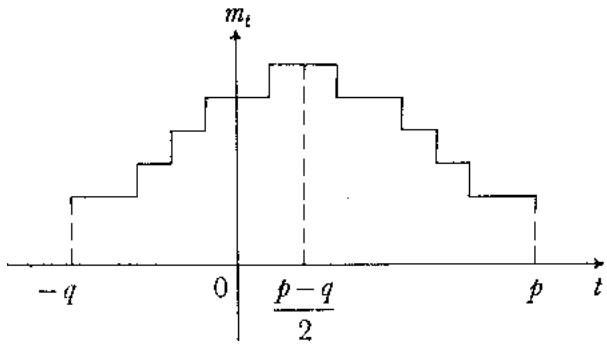
\includegraphics[keepaspectratio]{images/part001_39d2730e.jpg}}

（§1，第 2 节，命题 2）。由此可得：\(\mathrm{V}^{\lambda + t\alpha} \neq 0\)，只要 \(p \geq t \geq p - (\lambda(H_{\alpha}) + 2p)\)，所以 \(p + q \geq \lambda(H_{\alpha}) + 2p\)。将这个结果应用于 \(-\alpha\)，得到

\[
p + q \geq \lambda (H _ {- \alpha}) + 2 q = - \lambda (H _ {\alpha}) + 2 q.
\]

因此 \(q - p = \lambda (H_{\alpha})\)，且 \(\lambda + t\alpha \in \mathcal{X}\)（当 \(p \geq t \geq -q\) 时），这证明了 (i)。

我们有 \(s_{\alpha}(\alpha) = -\alpha\)，且 \(s_{\alpha}(\mu) \in \mu + k\alpha\) 对所有 \(\mu \in \mathfrak{h}^*\) 成立。由于 W 使 \(\mathcal{X}\) 保持稳定（命题 2 的推论 2），\(s_{\alpha}\) 使 \(\{\lambda - q\alpha, \lambda - q\alpha + \alpha, \ldots, \lambda + p\alpha\}\) 保持稳定，并将 \(\lambda - q\alpha + u\alpha\) 映到 \(\lambda + p\alpha - u\alpha\)，其中对所有 \(u \in k\) 都成立。再次使用命题 2 的推论 2，可见 \(m_{-q + u} = m_{p - u}\)，其中 \(u \in [0, p + q]\) 为任意整数。这证明了 (ii)。

根据 §1，命题 2 的推论，\((X_{\alpha})_{\mathrm{V}}|\mathrm{V}^{\lambda +t\alpha}\) 在 \(t < (p - q) / 2\) 时是单射。现在 \((X_{\alpha})_{\mathrm{V}}\) 将 \(\mathrm{V}^{\lambda +t\alpha}\) 映到 \(\mathrm{V}^{\lambda +(t + 1)\alpha}\)。所以 \(m_{t + 1}\geq m_t\)，只要 \(t < (p - q) / 2\)。将 \(\alpha\) 换成 \(-\alpha\)，可见 \(m_{t + 1}\leq m_t\)，只要 \(t > (p - q) / 2\)。这证明了 (iii) 和 (iv)。

推论 1. 若 \(\lambda \in \mathcal{X}\) 且 \(\lambda (H_{\alpha})\geq 1\)，则 \(\lambda -\alpha \in \mathcal{X}\)。若 \(\lambda +\alpha \in \mathcal{X}\) 且 \(\lambda (H_{\alpha}) = 0\)，则 \(\lambda \in \mathcal{X}\) 且 \(\lambda -\alpha \in \mathcal{X}\)。

这立即由命题 3 (i) 得出。

推论 2. 设 \(\mu \in \mathrm{P}_{++}\) 且 \(\nu \in \mathrm{Q}_{+}\)。若 \(\mu + \nu \in \mathcal{X}\)，则 \(\mu \in \mathcal{X}\)。

写成 \(\nu = \sum_{\alpha \in \mathrm{B}} c_{\alpha}.\alpha\)，其中 \(c_{\alpha} \in \mathbf{N}\) 对所有 \(\alpha \in \mathrm{B}\) 成立。当 \(\sum_{\alpha \in \mathrm{B}} c_{\alpha} = 0\) 时推论显然成立；假设 \(\sum_{\alpha \in \mathrm{B}} c_{\alpha} > 0\)，并对 \(\sum_{\alpha \in \mathrm{B}} c_{\alpha}\) 作归纳。设 \((\cdot|\cdot)\) 是 \(\mathfrak{h}_{\mathbf{R}}^{*}\) 上 W-不变的非退化正对称双线性型。于是 \((\nu|\sum_{\alpha \in \mathrm{B}} c_{\alpha}.\alpha) > 0\)，所以存在 \(\beta \in \mathrm{B}\)，使得 \(c_{\beta} \geq 1\) 且 \((\nu|\beta) > 0\)，从而 \(\nu(H_{\beta}) \geq 1\)。由于 \(\mu \in \mathrm{P}_{++}\)，可得 \((\mu + \nu)(H_{\beta}) \geq 1\)。根据推论 1，\(\mu + (\nu - \beta) \in \mathcal{X}\)，于是只需应用归纳假设。

推论 3. 设 \(v \in V\) 是权为 \(\omega\) 的本原元。设 \(\Sigma\) 为满足 \(\alpha \in B\) 且 \(\omega(H_{\alpha}) = 0\) 的元素所成的集合。\(\mathfrak{g}\) 中直线 \(kv\) 的稳定子是抛物子代数 \(\mathfrak{p}_{\Sigma}\)，它对应于 \(\Sigma\)（§3，第 4 节，备注）。

必要时以 v 生成的 g-子模替换 V，于是可假设 V 是单模。设 s 为稳定子。我们有 \((\mathfrak{n}_{+})_{\mathrm{V}}v = 0\)，\((\mathfrak{h})_{\mathrm{V}}v \subset kv\)。设 \(\alpha \in B\) 满足 \(\omega(H_{\alpha}) = 0\)。我们有 \(\omega + \alpha \notin X\)，从而 \(\omega - \alpha \notin X\)（命题 3 (i)），因而 \((\mathfrak{g}^{-\alpha})_{\mathrm{V}}v = 0\)。前述结果说明 \(p_{\Sigma} \subset s\)。若 \(p_{\Sigma} \neq s\)，则 \(s = p_{\Sigma'}\)，其中 \(\Sigma'\) 是严格包含 \(\Sigma\) 的 B 的子集。设 \(\beta \in \Sigma' - \Sigma\)。于是 \(g^{-\beta}\) 稳定 kv，因而湮灭 v。但是，由于 \(\omega(H_{\beta}) > 0\)，这与命题 3 (iii) 矛盾。证毕。

P 的一个子集 \(\mathcal{X}\) 称为 R-饱和的，如果满足以下条件：对所有 \(\lambda \in \mathcal{X}\) 和所有 \(\alpha \in \mathrm{R}\)，有 \(\lambda - t\alpha \in \mathcal{X}\)，其中 \(t\) 遍历 0 与 \(\lambda(H_{\alpha})\) 之间的所有整数。由于 \(s_{\alpha}(\lambda) = \lambda - \lambda(H_{\alpha})\alpha\)，可见 P 的 R-饱和子集在 W 下稳定。设 \(\mathcal{Y} \subset \mathrm{P}\)。\(\lambda\) 是 \(\mathcal{Y}\) 的一个元素，在 \(\mathcal{Y}\) 中称为 R-极值元，如果对所有 \(\alpha \in \mathrm{R}\)，都有 \(\lambda + \alpha \notin \mathcal{Y}\) 或 \(\lambda - \alpha \notin \mathcal{Y}\)。

命题 4. 设 \(\mathrm{V}\) 是有限维 \(\mathfrak{g}\)-模，\(d\) 是满足 \(\geq 1\) 的整数。\(\mathrm{V}\) 中重数 \(\geq d\) 的权的集合是 R-饱和的。

这立即由命题 3 得出。

命题 5. 设 V 是有限维单 g-模，\(\omega\) 是其最高权，X 是其权集。取双线性型 \((\cdot|\cdot)\)，它定义在 \(h_{R}^{*}\) 上，且 W-不变、非退化、正定；并令 \(\lambda\mapsto\|\lambda\|=(\lambda|\lambda)^{1/2}\) 为相应的范数。

\begin{enumerate}
\def\labelenumi{(\roman{enumi})}
\item
  \(\mathcal{X}\) 是包含 \(\omega\) 的 P 的最小 R-饱和子集。
\item
  \(\mathcal{X}\) 的 R-极值元正是 \(\omega\) 在 W 下的变换。
\item
  若 \(\mu \in \mathcal{X}\)，则 \(\| \mu \| \leq \| \omega \|\)。此外，若 \(\mu \neq \omega\)，则 \(\| \mu + \rho \| < \| \omega + \rho \|\)。若 \(\mu\) 不是 \(\mathcal{X}\) 中的 R-极值元，则 \(\| \mu \| < \| \omega \|\)。
\item
  我们有 \(\mathcal{X} = \mathrm{W.}(\mathcal{X}\cap \mathrm{P}_{++})\)。其中，\(\lambda\) 是 \(\mathrm{P}_{++}\) 中的元素；其属于 \(\mathcal{X}\cap \mathrm{P}_{++}\) 当且仅当 \(\omega -\lambda \in \mathrm{Q}_{+}\)。
\item
  设 \(\mathcal{X}'\) 是包含 \(\omega\) 的 P 的最小 R-饱和子集。我们有 \(\mathcal{X}' \subset \mathcal{X}\)（命题 4）。假设 \(\mathcal{X} \neq \mathcal{X}'\)。设 \(\lambda\) 是 \(\mathcal{X} - \mathcal{X}'\) 的极大元。由于 \(\lambda \neq \omega\)，存在 \(\alpha \in B\)，使得 \(\lambda + \alpha \in \mathcal{X}\)。按命题 3 引入 \(p\) 和 \(q\)。由于 \(\lambda\) 是 \(\mathcal{X} - \mathcal{X}'\) 中的极大元，\(\lambda + p\alpha \in \mathcal{X}'\)。根据命题 3 (ii)，\(\lambda - q\alpha \in \mathcal{X}'\)，因为 \(\mathcal{X}'\) 在 W 下稳定。因此，有 \(\lambda + u\alpha \in \mathcal{X}'\)，其中 \(u\) 遍历区间 \([-q, p]\) 中的每个整数。这与 \(\lambda \notin \mathcal{X}'\) 矛盾，从而证明了 (i)。
\item
  显然，\(\omega\) 是 \(\mathcal{X}\) 中的 R-极值元；因此它在 W 下的变换也都是 \(\mathcal{X}\) 中的 R-极值元。设 \(\lambda\) 是 \(\mathcal{X}\) 中的 R-极值元；我们将证明 \(\lambda \in \mathrm{W}.\omega\)。由于存在 \(w \in \mathrm{W}\)，使得 \(w\lambda \in \mathrm{P}_{++}\)（第 VI 章，§1，第 10 节），不妨设 \(\lambda \in \mathrm{P}_{++}\)。设 \(\alpha \in \mathrm{B}\)；按命题 3 引入 \(p\) 和 \(q\)。由于 \(\lambda\) 是 R-极值元，\(p = 0\) 或 \(q = 0\)。由于
\end{enumerate}

\[
q - p = \lambda (H _ {\alpha}) \geq 0,
\]

不可能有 \(p > 0\)。因此 \(p = 0\) 且 \(\lambda = \omega\)。

\begin{enumerate}
\def\labelenumi{(\roman{enumi})}
\setcounter{enumi}{2}
\tightlist
\item
  设 \(\mu \in \mathcal{X} \cap \mathrm{P}_{++}\)。则 \(\omega + \mu \in \mathrm{P}_{++}\) 且 \(\omega - \mu \in \mathrm{Q}_+\)（§6，第 1 节，命题 1），所以 \(0 \leq (\omega - \mu|\omega + \mu) = (\omega|\omega) - (\mu|\mu)\)；从而 \((\mu|\mu) \leq (\omega|\omega)\)，利用 Weyl 群可将此结论推广到所有 \(\mu \in \mathcal{X}\)。如果 \(\mu \in \mathcal{X} - \{\omega\}\)，
\end{enumerate}

\[
\begin{array}{c} (\mu + \rho | \mu + \rho) = (\mu | \mu) + 2 (\mu | \rho) + (\rho | \rho) \leq (\omega | \omega) + 2 (\mu | \rho) + (\rho | \rho) \\ = (\omega + \rho | \omega + \rho) - 2 (\omega - \mu | \rho). \end{array}
\]

现在 \(\omega - \mu = \sum_{\alpha \in \mathrm{B}} n_{\alpha} \alpha\)，其中整数 \(n_{\alpha} \geq 0\) 不全为零，所以 \((\omega - \mu | \rho) > 0\)，因为 \((\rho | \alpha) > 0\) 对所有 \(\alpha \in \mathrm{B}\) 都成立（第 VI 章，§1，第 10 节，命题 29 (iii)）。若 \(\mu\) 不是 \(\mathcal{X}\) 中的 R-极值元，则存在 \(\alpha \in \mathrm{R}\)，使得 \(\mu + \alpha \in \mathcal{X}\) 且 \(\mu - \alpha \in \mathcal{X}\)；于是

\[
\| \mu \| <   \sup (\| \mu + \alpha \|, \| \mu - \alpha \|) \leq \sup _ {\lambda \in \mathcal {X}} \| \lambda \|
\]

而根据前述结果，这个上界是 \(\|\omega\|\)。

\begin{enumerate}
\def\labelenumi{(\roman{enumi})}
\setcounter{enumi}{3}
\tightlist
\item
  根据第 VI 章，§1，第 10 节，我们有 \(\mathcal{X} = \mathrm{W.}(\mathcal{X}\cap \mathrm{P}_{++})\)。若 \(\lambda \in \mathcal{X}\)，则 \(\omega -\lambda \in \mathrm{Q}_{+}\)（§6，第 1 节，命题 1）。若 \(\lambda \in \mathrm{P}_{++}\) 且 \(\omega -\lambda \in \mathrm{Q}_{+}\)，则 \(\lambda \in \mathcal{X}\)（命题 3 的推论 2）。
\end{enumerate}

推论。设 X 是 P 的有限 R-饱和子集。存在一个权集为 X 的有限维 g-模。

由于 \(\mathcal{X}\) 在 W 下稳定，\(\mathcal{X}\) 是包含 \(\mathcal{X} \cap \mathrm{P}_{++}\) 的最小 R-饱和集。根据命题 5 (i)，\(\mathcal{X}\) 是 \(\bigoplus_{\lambda \in \mathcal{X} \cap \mathrm{P}_{++}} \mathrm{E}(\lambda)\) 的权集。

备注 2. 回顾一下（第 VI 章，§1，第 6 节，命题 17 的推论 3），存在唯一的 \(w_0\)，它是 \(\mathrm{W}\) 中将 \(\mathrm{B}\) 变为 \(-\mathrm{B}\) 的元素；我们有 \(w_0^2 = 1\)。并且 \(-w_0\) 保持 \(\mathrm{P}\) 上的序关系。记 \(\mathrm{V}\) 为有限维单 \(\mathfrak{g}\)-模，\(\omega\) 为其最高权。则 \(w_0(\omega)\) 是 \(\mathrm{V}\) 的最低权，且其重数为 1。

\subsection{极小权}

命题 6. 设 \(\lambda \in \mathrm{P}\)，\(\mathcal{X}\) 是包含 \(\lambda\) 的 P 的最小 R-饱和子集。取如命题 5 中的范数 \(\| \cdot \|\)。以下条件等价：

\begin{enumerate}
\def\labelenumi{(\roman{enumi})}
\item
  \(\mathcal{X} = \mathrm{W}.\lambda\) ;
\item
  \(\mathcal{X}\) 的所有元素具有相同的范数；
\item
  对所有 \(\alpha \in \mathrm{R}\)，都有 \(\lambda(H_{\alpha}) \in \{0,1,-1\}\)。
\end{enumerate}

P 的每个非空 R-饱和子集都包含一个满足上述条件的元素 \(\lambda\)。

引入条件：

（ii'）对所有 \(\alpha \in \mathrm{R}\)，设 \(t\) 为介于 0 与 \(\lambda(H_{\alpha})\) 之间的任一整数，

\[
\| \lambda - t \alpha \| \geq \| \lambda \|.
\]

\begin{enumerate}
\def\labelenumi{(\roman{enumi})}
\tightlist
\item
  \(\Longrightarrow\) (ii) \(\Longrightarrow\) (ii')：显然。
\end{enumerate}

\((\mathrm{ii}^{\prime}) \Longrightarrow (\mathrm{iii})\)：假设条件 \((\mathrm{ii}^{\prime})\) 满足。设 \(\alpha \in \mathrm{R}\)。我们有 \(\| \lambda \| = \| \lambda - \lambda (H_{\alpha})\alpha \|\)，所以有 \(\| \lambda - t\alpha \| < \| \lambda \|\)，其中 \(t\) 严格位于 0 与 \(\lambda (H_{\alpha})\) 之间；因此不存在这样的整数，从而 \(|\lambda (H_{\alpha})| \leq 1\)。

\begin{enumerate}
\def\labelenumi{(\roman{enumi})}
\setcounter{enumi}{2}
\tightlist
\item
  \(\Longrightarrow\) (i)：假设条件 (iii) 满足。设 \(w \in W\) 且 \(\alpha \in R\)。则 \((w\lambda)(H_{\alpha}) = \lambda(H_{w^{-1}\alpha}) \in \{0,1,-1\}\)；因此，若 t 是介于 0 与 \((w\lambda)(H_{\alpha})\) 之间的整数，则 \(w\lambda - t\alpha\) 等于 \(w\lambda\) 或 \(s_{\alpha}(w\lambda)\)。这证明 W. \(\lambda\) 是 R-饱和的，所以 X = W. \(\lambda\)。
\end{enumerate}

设 Y 是 P 的非空 R-饱和子集。Y 中存在一个范数最小的元素 \(\lambda\)。显然 \(\lambda\) 满足条件 (ii')，从而得到命题的最后一个断言。

命题 7. 设 V 是有限维单 g-模，X 是 V 的权集，\(\lambda\) 是 X 的最高元（参见命题 5 (i)）。命题 6 的条件 (i)、(ii) 和 (iii) 等价于：

\begin{enumerate}
\def\labelenumi{(\roman{enumi})}
\setcounter{enumi}{3}
\tightlist
\item
  对所有 \(\alpha \in \mathrm{R}\) 以及所有 \(x \in \mathfrak{g}^{\alpha}\)，都有 \((x_{\mathrm{V}})^2 = 0\)。
\end{enumerate}

若这些条件满足，则 V 的所有权的重数都为 1。

若 (i) 满足，则 \(X = W \cdot \lambda\)，且所有权都与 \(\lambda\) 具有相同的重数（命题 2 的推论 2），换言之，重数为 1。此外，若 \(w \in W\) 且 \(\alpha \in R\)，则 \(w\lambda + t\alpha\) 是 V 的权必有 \(|t| \leq 1\)。因此，若 \(x \in g^{\alpha}\)，

\[
(x _ {\mathrm{V}}) ^ {2} (\mathrm{V} ^ {w (\lambda)}) \subset \mathrm{V} ^ {w (\lambda) + 2 \alpha} = 0,
\]

所以 \((x_{\mathrm{V}})^2 = 0\)，这证明了 (i) \(\Longrightarrow\) (iv)。

反过来，假设 (iv) 满足。设 \(\alpha \in \mathrm{R}\)，并给 V 赋予 \(\mathfrak{sl}(2,k)\)-模结构，定义此结构的元素为 \(X_{\alpha}, X_{-\alpha}, H_{\alpha}\)，这些元素属于 \(\mathfrak{g}\)。将 (iv) 应用于 \(x = X_{\alpha}\)，可知 \(\mathfrak{sl}(2,k)\)-模 V 的权属于 \(\{0,1,-1\}\)（参见 §1，第 2 节，命题 2 的推论）。特别地，\(\lambda(H_{\alpha}) \in \{0,1,-1\}\)，所以 (iv) \(\Longrightarrow\) (iii)。

命题 8. 假设 g 是单的。以 \(\alpha_{1},\ldots,\alpha_{l}\) 表示 B 的元素。设 \(\varpi_{1},\ldots,\varpi_{l}\) 是相应的基本权。设 \(H = n_{1}H_{\alpha_{1}} + \cdots + n_{l}H_{\alpha_{l}}\) 是 \(R^{\vee}\) 的最高根，J 是这样的 \(i \in \{1,\ldots,l\}\) 的集合：满足 \(n_{i} = 1\)。设 \(\lambda \in P_{++} - \{0\}\)。则命题 6 的条件 (i)、(ii) 和 (iii) 分别等价于以下每个条件：

\begin{enumerate}
\def\labelenumi{(\alph{enumi})}
\setcounter{enumi}{21}
\tightlist
\item
  \(\lambda(H)=1;\)
\end{enumerate}

\begin{enumerate}
\def\labelenumi{(\roman{enumi})}
\setcounter{enumi}{5}
\tightlist
\item
  存在 \(i \in \mathrm{J}\)，使得 \(\lambda = \varpi_i\)。
\end{enumerate}

\(\varpi_{i}\)（其中 \(i \in J\)）在 P(R) 中构成 P(R)/Q(R) 的非零元素的一个代表系。

设 \(\lambda = u_{1}\varpi_{1} + \cdots + u_{l}\varpi_{l}\)，其中 \(u_{1}, \ldots, u_{l}\) 是满足 \(\geq 0\) 且不全为零的整数。则 \(\lambda(H) = u_{1}n_{1} + \cdots + u_{l}n_{l}\)，且 \(n_{1} \geq 1, \ldots, n_{l} \geq 1\)，这立即给出 (v) 与 (vi) 的等价性。另一方面，\(\lambda(H) = \sup_{\alpha \in \mathrm{R}_{+}} \lambda(H_{\alpha})\)，且 \(\lambda(H) > 0\)，因为 \(\lambda\) 是 \(P_{++}\) 的非零元素。因此，条件 (v) 等价于条件 \(\lambda(H_{\alpha}) \in \{0, 1\}\) 对所有 \(\alpha \in R\) 成立，换言之，等价于命题 6 的条件 (iii)。

命题的最后一个断言由第 VI 章，§2，第 3 节，命题 6 的推论得出。

定义 1. 假设 \(\mathfrak{g}\) 是单的。\((\mathfrak{g},\mathfrak{h})\) 的极小权是 \(\mathrm{P}_{++} - \{0\}\) 中满足命题 6、7 和 8 的等价条件 (i)、(ii)、(iii)、(iv)、(v) 和 (vi) 的元素。

备注。假设 g 是单的。设 \(\Sigma^{\prime\vee}\) 是仿射 Weyl 群 \(\mathrm{W}_{a}(\mathrm{R}^{\vee})\) 的 Coxeter 图。回顾一下，\(\Sigma^{\prime\vee}\) 的顶点是 Coxeter 图 \(\Sigma^{\vee}\)（即 \(\mathrm{W}(\mathrm{R}^{\vee})\) 的 Coxeter 图）的顶点，再加上一个补充顶点 0。群 \(\mathrm{A}(\mathrm{R}^{\vee})\) 作用于 \(\Sigma^{\prime\vee}\)，并固定 0。群 \(\mathrm{Aut}(\Sigma^{\prime\vee})\) 典则同构于 \(\mathrm{A}(\mathrm{R}^{\vee})/\mathrm{W}(\mathrm{R}^{\vee})\) 与群 \(\Gamma_{C}\) 的半直积（参见第 VI 章，§2，第 3 节以及第 VI 章，§4，第 3 节）；显然 \((\operatorname{Aut} \Sigma'^{\vee})(0) = \Gamma_C(0)\)；并且 \(\Gamma_C(0)\) 由 0 以及 \(\Sigma^{\vee}\) 中与 \(\varpi_i\)（其中 \(i \in \mathbf{J}\)）对应的顶点组成（参见第 VI 章，§2，命题 5 以及第 3 节的备注 1）。总之，极小权是与 \(\Sigma^{\vee}\) 中可由 \(\operatorname{Aut}(\Sigma'^{\vee})\) 的某个元素作用于 0 而得到的顶点相对应的基本权。

采用第 VI 章图版 I 至 IX 的记号，由前述结果可推出，极小权如下：

对于 \(A_{l}\) 型（\(l \geq 1\)）：\(\varpi_{1}, \ldots, \varpi_{l}\)。

对于 \(B_{l}\) 型（\(l \geq 2\)）：\(\varpi_{l}\)。

对于 \(C_{l}\) 型（\(l \geq 2\)）：\(\varpi_{1}\)。

对于 \(D_{l}\) 型（\(l \geq 3\)）：\(\varpi_{1}, \varpi_{l-1}, \varpi_{l}\)。

对于 \(E_{6}\) 型：\(\varpi_{1}, \varpi_{6}\)。

对于 \(\mathrm{E}_7\) 型：\(\varpi_7\)。

对于 \(E_{8}, F_{4}, G_{2}\) 型，不存在极小权。

\subsection{g-模的张量积}

设 \(\mathrm{E},\mathrm{F}\) 为 \(\mathfrak{g}\)-模。对于所有 \(\lambda, \mu \in \mathfrak{h}^*\)，有 \(\mathrm{E}^\lambda \otimes \mathrm{F}^\mu \subset (\mathrm{E} \otimes \mathrm{F})^{\lambda + \mu}\)（第 VII 章，§1，第 1 节，命题 2 (ii)）。若 \(\mathrm{E}\) 和 \(\mathrm{F}\) 是有限维的，则 \(\mathrm{E} = \sum_{\lambda \in \mathrm{P}} \mathrm{E}^\lambda\) 且 \(\mathrm{F} = \sum_{\mu \in \mathrm{P}} \mathrm{F}^\mu\)；因此，

\[
(\mathrm{E} \otimes \mathrm{F}) ^ {\nu} = \sum_ {\lambda , \mu \in \mathrm{P}, \lambda + \mu = \nu} \mathrm{E} ^ {\lambda} \otimes \mathrm{F} ^ {\mu}.
\]

换言之，赋予 \(E \otimes F\) 其 P 型分次后，它是分次向量空间 E 和 F 的分次张量积。

命题 9. 设 E、F 是有限维单 g-模，最高权分别为 \(\lambda,\mu\)。

\begin{enumerate}
\def\labelenumi{(\roman{enumi})}
\item
  \(\mathrm{E} \otimes \mathrm{F}\) 中最高权为 \(\lambda + \mu\) 的分量是一个单子模，由 \((\mathrm{E} \otimes \mathrm{F})^{\lambda + \mu} = \mathrm{E}^{\lambda} \otimes \mathrm{F}^{\mu}\) 生成。
\item
  \(\mathrm{E} \otimes \mathrm{F}\) 的任意单子模的最高权都 \(\leq \lambda + \mu\)（参见 §9，命题 2）。
\end{enumerate}

若 \(\alpha, \beta \in \mathrm{P}\) 且 \(\mathrm{E}^{\alpha} \otimes \mathrm{F}^{\beta} \neq 0\)，则 \(\alpha \leq \lambda\) 且 \(\beta \leq \mu\)。因此，\((\mathrm{E} \otimes \mathrm{F})^{\lambda + \mu}\) 等于 \(\mathrm{E}^{\lambda} \otimes \mathrm{F}^{\mu}\)，从而维数为 1，而 \(\lambda + \mu\) 是 \(\mathrm{E} \otimes \mathrm{F}\) 的最高权。 \(\mathrm{E}^{\lambda} \otimes \mathrm{F}^{\mu}\) 的每个非零元素都是本原元。根据 §6 第 2 节的命题 4，\(\mathrm{E} \otimes \mathrm{F}\) 中最高权为 \(\lambda + \mu\) 的同构型分支的长度为 1。

备注。保留命题 9 的记号。设 C 是 \(E \otimes F\) 中最高权为 \(\lambda + \mu\) 的同构型分支。则 C 只依赖于 E 和 F，而不依赖于 h 和基 B 的选择。换言之，设 \(h'\) 是 g 的一个分裂嘉当子代数，\(R'\) 是 \((\mathfrak{g}, \mathfrak{h}')\) 的根系，\(B'\) 是 \(R'\) 的一个基；设 \(\lambda', \mu'\) 是 E、F 关于 \(h'\) 和 \(B'\) 的最高权；设 \(C'\) 是 \(E \otimes F\) 中最高权为 \(\lambda' + \mu'\) 的同构型分支；则 \(C' = C\)。事实上，为证明这一点，可以通过扩张基域假设 k 是代数闭域。于是存在 \(s \in \operatorname{Aut}_{e}(\mathfrak{g})\)，将 \(h\) 映到 \(h'\)，将 R 映到 \(R'\)，将 B 映到 \(B'\)。设 \(S \in \mathbf{SL}(E \otimes F)\) 具有第 1 节命题 2 中的性质。于是 \(\mathrm{S}((\mathrm{E} \otimes \mathrm{F})^{\lambda + \mu}) = (\mathrm{E} \otimes \mathrm{F})^{\lambda' + \mu'}\)，且 \(\mathrm{S}(\mathrm{C}) = \mathrm{C}\)。因此 \((\mathrm{E} \otimes \mathrm{F})^{\lambda' + \mu'} \subset \mathrm{C}' \cap \mathrm{S}(\mathrm{C}) = \mathrm{C}' \cap \mathrm{C}\)，所以 \(C' = C\)。这样，两个有限维单 g-模的同构类可典则地确定第三个同构类；换言之，我们在有限维单 g-模的同构类集合 \(S_{g}\) 上定义了一个复合律。在此结构下，\(S_{g}\) 典则同构于加法幺半群 \(P_{++}\)。

推论 1. 设 \((\varpi_{\alpha})_{\alpha \in \mathrm{B}}\) 是关于 B 的基本权族。设 \(\lambda = \sum_{\alpha \in \mathrm{B}} m_{\alpha} \varpi_{\alpha} \in \mathrm{P}_{++}\)。对于所有 \(\alpha \in \mathrm{B}\)，设 \(\mathrm{E}_{\alpha}\) 是单 \(\mathfrak{g}\)-模，其最高权为 \(\varpi_{\alpha}\)。在 \(\mathfrak{g}\)-模 \(\bigotimes_{\alpha \in \mathrm{B}} (\bigotimes^{m_{\alpha}} \mathrm{E}_{\alpha})\) 中，最高权为 \(\lambda\) 的同构型分支长度为 1。

这由命题 9 对 \(\sum_{\alpha \in \mathrm{B}}m_{\alpha}\) 作归纳得到。

推论 2. 假设 k 是 R、C 或非离散完备超度量域。设 G 是李代数为 g 的李群。假设对于 g 的任意基本表示 \(\rho\)，都存在 G 的一个解析线性表示 \(\rho'\)，使得 \(\rho = \mathrm{L}(\rho')\)。那么对于 g 的任意有限维线性表示 \(\pi\)，都存在 G 的一个解析线性表示 \(\pi'\)，使得 \(\pi = \mathrm{L}(\pi')\)。

使用推论 1 的记号。存在一个 G 的表示 \(\sigma\)，作用在 \(X = \bigotimes_{\alpha \in B} (\bigotimes^{m_{\alpha}} E_{\alpha})\) 上，使得 \(L(\sigma)\) 对应于 X 的 \(\mathfrak{g}\)-模结构（第 III 章，§3，第 11 节，命题 41 的推论 3）。设 C 是 X 中最高权为 \(\lambda\) 的同构型分支。根据第 III 章，§3，第 11 节，命题 40，只需证明 C 在 \(\sigma(G)\) 下稳定。设 \(g \in G\)，且 \(\varphi = \operatorname{Ad}(g)\)。则 \(\sigma(g)a_X \sigma(g)^{-1} = (\varphi(a))_X\) 对所有 \(a \in \mathfrak{g}\) 成立。另一方面，\(\varphi\) 是 \(\mathfrak{g}\) 的一个自同构，将 \(\mathfrak{h}\) 映到 \(\mathfrak{h}'\)，将 R 映到 \(R' = R(\mathfrak{g}, \mathfrak{h}')\)，将 B 映到 \(B'\)，它是 \(R'\) 的一个基，并将 \(\varpi_{\alpha}\) 映到 \(\varpi_{\alpha}'\)，即 \(E_{\alpha}\) 关于 \(\mathfrak{h}'\) 和 \(B'\) 的最高权（因为 \(\varphi\) 将 \(E_{\alpha}\) 变为一个 \(\mathfrak{g}\)-模，该模与 \(E_{\alpha}\) 同构）。因此 \(\varphi\) 将 \(\lambda\) 映到 \(\sum m_{\alpha} \varpi_{\alpha}'\)。根据上面的备注，\(\sigma(g)(C) = C\)。

命题 10. 设 \(\lambda, \mu \in \mathrm{P}_{++}\)。设 E、F、G 是单 \(\mathfrak{g}\)-模，其最高权分别为 \(\lambda, \mu, \lambda + \mu\)。设 \(\mathcal{X}\)（分别为 \(\mathcal{X}', \mathcal{X}''\)）是 E（分别为 F、G）的权集。则 \(\mathcal{X}'' = \mathcal{X} + \mathcal{X}'\)。

我们有 \(E = \bigoplus_{\nu \in P} E^{\nu}, F = \bigoplus_{\sigma \in P} F^{\sigma}\)，所以 \(E \otimes F\) 是下列各空间的直和

\[
(\mathrm{E} \otimes \mathrm{F}) ^ {\tau} = \sum_ {\nu + \sigma = \tau} \mathrm{E} ^ {\nu} \otimes \mathrm{F} ^ {\sigma}.
\]

根据命题 9，\(\mathbf{G}\) 可识别为一个 \(\mathfrak{g}\)-子模，并且它包含在 \(\mathrm{E} \otimes \mathrm{F}\) 中，因此 \(\mathcal{X}'' \subset \mathcal{X} + \mathcal{X}'\)。我们有 \(\mathrm{G}^{\tau} = \mathrm{G} \cap (\mathrm{E} \otimes \mathrm{F})^{\tau}\)，只需证明：对于 \(\nu \in \mathcal{X}\) 和 \(\sigma \in \mathcal{X}'\)，有 \(\mathrm{G} \cap (\mathrm{E} \otimes \mathrm{F})^{\nu + \sigma} \neq 0\)。设 \((e_1, \ldots, e_n)\)（分别为 \((f_1, \ldots, f_p))\) 是 \(\mathrm{E}\)（分别为 \(\mathrm{F}\)）的一个基，其中每个基向量属于某个 \(\mathrm{E}^\nu\)（分别为 \(\mathrm{F}^\sigma\)），并且 \(e_1 \in \mathrm{E}^\lambda\)（分别为 \(f_1 \in \mathrm{F}^\mu\)）。\(e_i \otimes f_j\) 构成 \(\mathrm{E} \otimes \mathrm{F}\) 的一个基。假设要证明的结论不成立。则存在一对 \((i,j)\)，使得每个 \((i,j)\) 号坐标在 \(\mathrm{G}\) 的每个元素中都为零。设 \(\mathrm{U}\) 是 \(\mathfrak{g}\) 的包络代数，\(\mathrm{U}'\) 是 \(\mathrm{U}\) 的对偶，\(c\) 是 \(\mathrm{U}\) 的余积。对于所有 \(u \in \mathrm{U}\)，令 \(x_i(u)\)（分别为 \(y_j(u)\)）为 \(u(e_1)\)（分别为 \(u(f_1)\)）的 \(i\)（分别为 \(j\)）号坐标；令 \(z_{ij}(u)\) 为编号为 \((i,j)\) 的 \(u(e_1 \otimes f_1)\) 的坐标。于是 \(x_i, y_j, z_{ij} \in \mathrm{U}'\)。现在 \(e_1\) 生成 \(\mathfrak{g}\)-模 \(\mathrm{E}\)，所以 \(x_i \neq 0\)，同样 \(y_j \neq 0\)。根据 \(\mathfrak{g}\)-模 \(\mathrm{E} \otimes \mathrm{F}\) 的定义（第 I 章，§3，第 2 节），若 \(c(u) = \sum u_s \otimes u_s'\)，则有

\[
z _ {i j} (u) = \sum_ {s} x _ {i} (u _ {s}). y _ {j} (u _ {s} ^ {\prime}) = \langle c (u), x _ {i} \otimes y _ {j} \rangle .
\]

换言之，\(z_{ij}\) 是 \(x_{i}\) 与 \(y_{j}\) 在代数 \(U'\) 中的乘积。但这个代数是整环（第 II 章，§1，第 5 节，命题 10），所以 \(z_{ij} \neq 0\)。由于 \(u(e_{1} \otimes f_{1}) \in \mathrm{G}\) 对所有 \(u \in U\) 成立，这就矛盾了。

\subsection{g-模的对偶}

设 E、F 为 g-模。回顾一下（第 I 章，§3，第 3 节），\(\operatorname{Hom}_{k}(\operatorname{E},\operatorname{F})\) 具有典则的 g-模结构。设 \(\varphi\) 是权为 \(\lambda\) 的 \(\operatorname{Hom}_{k}(\operatorname{E},\operatorname{F})\) 中的元素。若 \(\mu \in h^{*}\)，则 \(\varphi(\operatorname{E}^{\mu}) \subset \operatorname{F}^{\lambda + \mu}\)（第 VII 章，§1，第 1 节，命题 2 (ii)）。因此，若 E 和 F 是有限维的，则权为 \(\lambda\) 的 \(\operatorname{Hom}_{k}(\operatorname{E},\operatorname{F})\) 中的元素，正是《代数》第 II 章 §11 第 2 节定义 4 意义下的次数为 \(\lambda\) 的分次同态。

命题 11. 设 E 是有限维 g-模，并考虑 g-模 \(E^{*} = \operatorname{Hom}_{k}(E, k)\)。

\begin{enumerate}
\def\labelenumi{(\roman{enumi})}
\item
  元素 \(\lambda \in \mathrm{P}\) 是 \(\mathrm{E}^*\) 的权，当且仅当 \(-\lambda\) 是 \(\mathrm{E}\) 的权；并且 \(\lambda\) 在 \(\mathrm{E}^*\) 中的重数等于 \(-\lambda\) 在 \(\mathrm{E}\) 中的重数。
\item
  若 \(\mathrm{E}\) 是最高权为 \(\omega\) 的单模，则 \(\mathrm{E}^*\) 是最高权为 \(-w_0(\omega)\) 的单模（参见第 2 节的备注 2）。
\end{enumerate}

把 k 看作元素权为 0 的平凡 g-模。根据上面的论述，\(E^{*}\) 中权为 \(\lambda\) 的元素，是从 E 到 k 的同态；它们在 \(E^{\mu}\) 上为零，只要 \(\mu \neq -\lambda\)。这证明了 (i)。若 E 是单模，则 \(E^{*}\) 也是单模（第 I 章，§3，第 3 节），最后一个断言由第 2 节的备注 2 得出。

备注。1) 设 E、E* 如命题 11 中，并设 \(\sigma \in \mathrm{Aut}(\mathfrak{g},\mathfrak{h})\) 满足，在 §5 第 1 节的记号下，\(\varepsilon (\sigma) = -w_0\)（§5，第 2 节，命题 2）。设 \(\rho ,\rho^{\prime}\) 是与 E、E* 相关的 \(\mathfrak{g}\) 表示。则 \(\rho \circ \sigma\) 是 \(\mathfrak{g}\) 的一个单表示，其最高权为 \(-w_{0}(\omega)\)，所以 \(\rho \circ \sigma\) 与 \(\rho^{\prime}\) 等价。

\begin{enumerate}
\def\labelenumi{\arabic{enumi})}
\setcounter{enumi}{1}
\tightlist
\item
  假设 \(w_{0} = -1\)。那么对于任意有限维 g-模 E，E 都同构于 \(E^{*}\)。回顾一下，若 g 是单的，则在以下情形中 \(w_{0} = -1\)：g 为 \(A_{1}, B_{l} (l \geq 2)\) 型、\(C_{l} (l \geq 2)\) 型、\(D_{l} (l \text{ even } \geq 4)\) 型，或 \(E_{7}, E_{8}, F_{4}, G_{2}\) 型（第 VI 章，图版）。
\end{enumerate}

引理 2. 令 \(h^0 = \sum_{\alpha \in \mathrm{R}_{+}} H_\alpha\)。则 \(h^0 = \sum_{\alpha \in \mathrm{B}} a_\alpha H_\alpha\)，其中 \(a_\alpha\) 是满足 \(\geq 1\) 的整数。设 \((b_\alpha)_{\alpha \in \mathrm{B}}, (c_\alpha)_{\alpha \in \mathrm{B}}\) 是满足 \(b_\alpha c_\alpha = a_\alpha\) 对所有 \(\alpha \in \mathrm{B}\) 成立的标量族。置 \(x = \sum_{\alpha \in \mathrm{B}} b_\alpha X_\alpha, y = \sum_{\alpha \in \mathrm{B}} c_\alpha X_{-\alpha}\)。存在一个同态 \(\varphi\)，从 \(\mathfrak{sl}(2,k)\) 到 \(\mathfrak{g}\)，使得 \(\varphi(H) = h^0, \varphi(X_+) = x, \varphi(X_-) = y\)。

事实 \(a_{\alpha}\) 是满足 \(\geq 1\) 的整数，是因为 \((H_{\alpha})_{\alpha \in \mathrm{B}}\) 是根系 \((H_{\alpha})_{\alpha \in \mathrm{B}}\) 的一个基（参见第 VI 章，§1，第 5 节，备注 5）。我们有：

\[
\alpha (h ^ {0}) = 2\tag{1}
\]

对所有 \(\alpha \in \mathrm{B}\) 都成立（第 VI 章，§1，第 10 节，命题 29 的推论），因此

\[
[ h ^ {0}, x ] = \sum_ {\alpha \in \mathrm{B}} b _ {\alpha} \alpha (h ^ {0}) X _ {\alpha} = 2 x\tag{2}
\]

\[
[ h ^ {0}, y ] = \sum_ {\alpha \in \mathrm{B}} c _ {\alpha} (- \alpha (h ^ {0})) X _ {- \alpha} = - 2 y.\tag{3}
\]

另一方面，

\[
[ x, y ] = \sum_ {\alpha , \beta \in \mathrm{B}} b _ {\alpha} c _ {\beta} [ X _ {\alpha}, X _ {- \beta} ] = \sum_ {\alpha \in \mathrm{B}} b _ {\alpha} c _ {\alpha} [ X _ {\alpha}, X _ {- \alpha} ] = - \sum_ {\alpha \in \mathrm{B}} a _ {\alpha} H _ {\alpha} = - h ^ {0},\tag{4}
\]

从而同态 \(\varphi\) 存在。

命题 12. 设 E 是有限维单 g-模，\(\omega\) 是其最高权，B 是 E 上 g-不变双线性型的向量空间。设 m 是整数 \(\sum_{\alpha\in\mathrm{R}_{+}}\omega(H_{\alpha})\)，从而 m/2 是 \(\omega\) 关于 B 的坐标之和（第 VI 章，§1，第 10 节，命题 29 的推论）。设 \(w_{0}\) 是满足 \(w_{0}(B) = -B\) 的 W 中的元素。

\begin{enumerate}
\def\labelenumi{(\roman{enumi})}
\item
  若 \(w_0(\omega) \neq -\omega\)，则 \(\mathcal{B} = 0\)。
\item
  假设 \(w_{0}(\omega) = -\omega\)。则 B 的维数为 1，且 B 的每个非零元素都是非退化的。若 m 为偶数（分别为奇数），则 B 的每个元素都是对称的（分别为交错的）。
\end{enumerate}

\begin{enumerate}
\def\labelenumi{\alph{enumi})}
\item
  设 \(\Phi \in \mathcal{B}\)。令 \(\varphi\) 为从 E 到 \(\mathrm{E}^*\) 的映射，对 \(x, y \in \mathrm{E}\) 定义为 \(\varphi(x)(y) = \Phi(x, y)\)；它是 \(\mathfrak{g}\)-模同态。若 \(\Phi \neq 0\)，则 \(\varphi \neq 0\)，所以根据 Schur 引理，\(\varphi\) 是同构，从而 \(\Phi\) 非退化。因此，\(\mathfrak{g}\)-模 E 同构于 \(\mathfrak{g}\)-模 \(\mathrm{E}^*\)，故 \(w_0(\omega) = -\omega\)。至此证明了 (i)。
\item
  从现在起假设 \(w_{0}(\omega) = -\omega\)。则 E 同构于 \(E^{*}\)。向量空间 B 同构于 \(\operatorname{Hom}_{\mathfrak{g}}(\mathrm{E}, \mathrm{E}^{*})\)，从而同构于 \(\operatorname{Hom}_{\mathfrak{g}}(\mathrm{E}, \mathrm{E})\)，后者的维数为 1（§6，第 1 节，命题 1 (iii)）。因此 \(\dim B = 1\)。根据 a)，B 的每个非零元素 \(\Phi\) 都是非退化的。令 \(\Phi_{1}(x, y) = \Phi(y, x)\)，其中 \(x, y \in E\)。由前述结果，存在 \(\lambda \in k\)，使得 \(\Phi_{1}(x, y) = \lambda \Phi(x, y)\) 对所有 \(x, y \in E\) 成立。于是 \(\Phi(y, x) = \lambda \Phi(x, y) = \lambda^{2} \Phi(y, x)\)，所以 \(\lambda^{2} = 1\) 且 \(\lambda = \pm 1\)。因此，\(\Phi\) 或者是对称的，或者是交错的。
\item
根据第 VII 章，§1，第 3 节，命题 9 (v)，\(E^{\lambda}\) 与 \(E^{\mu}\) 关于 \(\Phi\) 正交，只要 \(\lambda + \mu \neq 0\)。由于 \(\Phi\) 非退化，可知 \(E^{\omega}, E^{-\omega}\) 关于 \(\Phi\) 不正交。
\end{enumerate}

\(d\)）存在一个同态 \(\varphi\)，从 \(\mathfrak{sl}(2,k)\) 满射到 \(\mathfrak{g}\) 的某个子代数，并将 \(H\) 映到 \(\sum_{\alpha \in \mathrm{R}_{+}}H_{\alpha}\)（引理 2）。通过这个同态，把 E 看作一个 \(\mathfrak{sl}(2,k)\)-模。于是，\(\mathrm{E}^{\lambda}\) 的元素具有权 \(\lambda \left(\sum_{\alpha \in \mathrm{R}_{+}}H_\alpha\right)\)。若 \(\lambda \in \mathrm{P}\) 满足 \(\mathrm{E}^{\lambda} \neq 0\) 且 \(\lambda \neq \omega, \lambda \neq -\omega\)，则 \(-\omega < \lambda < \omega\)，所以

\[
- m = - \omega \left(\sum_ {\alpha \in \mathrm{R} _ {+}} H _ {\alpha}\right) <   \lambda \left(\sum_ {\alpha \in \mathrm{R} _ {+}} H _ {\alpha}\right) <   \omega \left(\sum_ {\alpha \in \mathrm{R} _ {+}} H _ {\alpha}\right) = m.
\]

令 \(G\) 为类型为 \(V(m)\) 的 \(\mathfrak{sl}(2, k)\)-模 \(E\) 的同构型分支。由上文，\(G\) 的长度为 1，且包含 \(E^{\omega}, E^{-\omega}\)。根据 \(c\)，\(\Phi\) 在 \(G\) 上的限制非零。根据 §1，第 3 项，备注 3，\(m\) 是偶数还是奇数，取决于这个限制是对称的还是交错的。鉴于 \(b\)，证毕。

定义 2. 若 g 的有限维不可约表示 \(\rho\) 在 E 上存在一个关于 \(\rho\) 不变的非退化对称（分别为交错）双线性型，则称该表示是正交型（分别为辛型）的。

\subsection{表示环}

设 \(\mathfrak{a}\) 是有限维李代数。设 \(\mathcal{F}_{\mathfrak{a}}\)（分别为 \(\mathfrak{S}_{\mathfrak{a}}\)）是有限维（分别为有限维单）\(\mathfrak{a}\)-模的同构类集合。设 \(\mathcal{R}(\mathfrak{a})\) 是自由阿贝尔群 \(\mathbf{Z}^{(\mathfrak{S}_{\mathfrak{a}})}\)。对于任意有限维单 \(\mathfrak{a}\)-模 E，以 {[}E{]} 表示其同构类。设 F 是有限维 \(\mathfrak{a}\)-模；设 \((\mathrm{F}_n,\mathrm{F}_{n - 1},\dots ,\mathrm{F}_0)\) 是 F 的 Jordan–Hölder 序列；则 \(\sum_{i = 1}^{n}[\mathrm{F}_i / \mathrm{F}_{i - 1}]\) 是 \(\mathcal{R}(\mathfrak{a})\) 中的元素，只依赖于 F，而不依赖于 Jordan–Hölder 序列的选择；我们将其记为 {[}F{]}。如果

\[
0 \longrightarrow \mathrm{F} ^ {\prime} \longrightarrow \mathrm{F} \longrightarrow \mathrm{F} ^ {\prime \prime} \longrightarrow 0
\]

是有限维 \(\mathfrak{a}\)-模的正合序列，则 \([\mathrm{F}] = [\mathrm{F}'] + [\mathrm{F}'']\)。

设 \(\mathrm{F}\) 是有限维半单 \(\mathfrak{a}\)-模；对于所有 \(\mathrm{E} \in \mathfrak{S}_{\mathfrak{a}}\)，设 \(n_{\mathrm{E}}\) 是 \(\mathrm{F}\) 中类型为 \(\mathrm{E}\) 的同构型分支的长度；则 \([\mathrm{F}] = \sum_{\mathrm{E} \in \mathfrak{S}_{\mathfrak{a}}} n_{\mathrm{E}}. \mathrm{E}\)。若 \(\mathrm{F}, \mathrm{F}'\) 是有限维半单 \(\mathfrak{a}\)-模，且 \([\mathrm{F}] = [\mathrm{F}']\)，则 \(\mathrm{F}\) 与 \(\mathrm{F}'\) 同构。

引理 3. 设 G 是用加法记号书写的阿贝尔群，\(\varphi : \mathcal{F}_{\mathfrak{a}} \to \mathrm{G}\) 是一个映射；略滥用记号，以 \(\varphi(\mathrm{F})\) 表示任意有限维模 F 的同构类在 \(\varphi\) 下的像，其中 F 是 \(\mathfrak{a}\)-模。假设对于任意正合序列

\[
0 \longrightarrow \mathrm{F} ^ {\prime} \longrightarrow \mathrm{F} \longrightarrow \mathrm{F} ^ {\prime \prime} \longrightarrow 0
\]

对于有限维 \(\mathfrak{a}\)-模，有 \(\varphi(\mathrm{F}) = \varphi(\mathrm{F}') + \varphi(\mathrm{F}'')\)。于是存在唯一的同态 \(\theta: \mathcal{R}(\mathfrak{a}) \to \mathrm{G}\)，使得 \(\theta([\mathrm{F}]) = \varphi(\mathrm{F})\) 对每个有限维 \(\mathfrak{a}\)-模 \(\mathrm{F}\) 成立。

存在唯一的同态 \(\theta\) 从 \(\mathcal{R}(\mathfrak{a})\) 到 G，使得对每个有限维单 a-模 E，都有 \(\theta([\mathrm{E}]) = \varphi(\mathrm{E})\)。设 F 是有限维 a-模，\((\mathrm{F}_{n}, \mathrm{F}_{n-1}, \ldots, \mathrm{F}_{0})\) 是 F 的 Jordan–Hölder 序列；若 \(n > 0\)，则对 n 作归纳可得

\[
\theta ([ \mathrm{F} ]) = \sum_ {i = 1} ^ {n} \theta ([ \mathrm{F} _ {i} / \mathrm{F} _ {i - 1} ]) = \sum_ {i = 1} ^ {n} \varphi (\mathrm{F} _ {i} / \mathrm{F} _ {i - 1}) = \varphi (\mathrm{F}).
\]

若 \(n = 0\)，则 \([\mathrm{F}] = 0\)，所以 \(\theta([\mathrm{F}]) = 0\)；另一方面，考察正合序列 \(0 \longrightarrow 0 \longrightarrow 0 \longrightarrow 0 \longrightarrow 0\)，可见 \(\varphi(0) = 0\)。

例。取 G = Z，且 \(\varphi(F) = \dim F\)。相应的从 \(\mathcal{R}(\mathfrak{a})\) 到 Z 的同态记为 dim。设 c 是一个维数为 1 的平凡 a-模的同构类，设 \(\psi\) 是由 \(n \mapsto nc\) 定义的同态，从 Z 到 \(\mathcal{R}(\mathfrak{a})\)。显然有

\(\dim \circ \psi = \operatorname{Id}_{\mathbf{Z}},\)

因此 \(\mathcal{R}(\mathfrak{a})\) 是 \(\operatorname{Kerdim}\) 与 \(\mathbf{Zc}\) 的直和。

引理 4. 在加法群 \(\mathcal{R}(\mathfrak{a})\) 上存在唯一的、关于加法可分配的乘法，使得 \([\mathrm{E}][\mathrm{F}] = [\mathrm{E}\otimes \mathrm{F}]\) 对所有有限维 \(\mathfrak{a}\)-模 E、F 成立。这样，\(\mathcal{R}(\mathfrak{a})\) 具有交换环的结构。维数为 1 的平凡 \(\mathfrak{a}\)-模的同构类是这个环的单位元。

唯一性显然。在 \(\mathcal{R}(\mathfrak{a}) = \mathbf{Z}^{(\mathfrak{S}_{\mathfrak{a}})}\) 上存在关于加法可分配的交换乘法，使得 \([E][F] = [E \otimes F]\) 对所有 \(E, F \in S_{a}\) 成立。设 \(E_{1}, E_{2}\) 是有限维 a-模，\(l_{1}\) 和 \(l_{2}\) 是它们的长度；我们证明 \([E_{1}][E_{2}] = [E_{1} \otimes E_{2}]\)，方法是对 \(l_{1} + l_{2}\) 作归纳。当 \(l_{1} + l_{2} \leq 2\) 时显然成立。另一方面，设 \(F_{1}\) 是 \(E_{1}\) 的一个既不为 0 也不为 \(E_{1}\) 的子模。于是

\[
[ \mathrm{F} _ {1} ] [ \mathrm{E} _ {2} ] = [ \mathrm{F} _ {1} \otimes \mathrm{E} _ {2} ] \text { and } [ \mathrm{E} _ {1} / \mathrm{F} _ {1} ] [ \mathrm{E} _ {2} ] = [ (\mathrm{E} _ {1} / \mathrm{F} _ {1}) \otimes \mathrm{E} _ {2} ]
\]

根据归纳假设。另一方面，\((\mathrm{E}_1\otimes \mathrm{E}_2) / (\mathrm{F}_1\otimes \mathrm{E}_2)\) 同构于 \((\mathrm{E}_1 / \mathrm{F}_1)\otimes \mathrm{E}_2\)。因此

\[
[ \mathrm{E} _ {1} ] [ \mathrm{E} _ {2} ] = ([ \mathrm{E} _ {1} / \mathrm{F} _ {1} ] + [ \mathrm{F} _ {1} ]). [ \mathrm{E} _ {2} ] = [ (\mathrm{E} _ {1} / \mathrm{F} _ {1}) \otimes \mathrm{E} _ {2} ] + [ \mathrm{F} _ {1} \otimes \mathrm{E} _ {2} ] = [ \mathrm{E} _ {1} \otimes \mathrm{E} _ {2} ],
\]

这就证明了我们的断言。立即可见，上面定义的乘法是结合的，所以 \(\mathcal{R}(\mathfrak{a})\) 具有交换环的结构。最后，显然维数为 1 的平凡 a-模的同构类是这个环的单位元。

引理 5. 存在唯一的对合自同构 \(\mathrm{X} \mapsto \mathrm{X}^*\)，定义在环 \(\mathcal{R}(\mathfrak{a})\) 上，使得 \([\mathrm{E}]^* = [\mathrm{E}^*]\) 对每个有限维 \(\mathfrak{a}\)-模 \(\mathrm{E}\) 成立。

唯一性显然。根据引理 3，存在一个同态 \(X \mapsto X^{*}\)，它把加法群 \(\mathcal{R}(\mathfrak{a})\) 映到自身，并满足 \([E]^{*} = [E^{*}]\) 对每个有限维 a-模 E 成立。我们有 \((X^{*})^{*} = X\)，所以这个同态是对合的。它是环 \(\mathcal{R}(\mathfrak{a})\) 的自同构，因为对于所有有限维 a-模 E、F，\((\mathrm{E} \otimes \mathrm{F})^{*}\) 同构于 \(E^{*} \otimes F^{*}\)。证毕。

设 \(\mathrm{U}(\mathfrak{a})\) 是 \(\mathfrak{a}\) 的包络代数，\(\mathrm{U}(\mathfrak{a})^*\) 是 \(\mathrm{U}(\mathfrak{a})\) 的向量空间对偶。回顾一下（第 II 章，§1，第 5 节），\(\mathrm{U}(\mathfrak{a})\) 的余代数结构在 \(\mathrm{U}(\mathfrak{a})^*\) 上定义了带单位元的交换结合代数结构。对于任意有限维 \(\mathfrak{a}\)-模 E，映射 \(u \mapsto \mathrm{Tr}(u_{\mathrm{E}})\) 从 \(\mathrm{U}(\mathfrak{a})\) 到 \(k\)，是元素 \(\tau_{\mathrm{E}}\)，属于 \(\mathrm{U}(\mathfrak{a})^*\)。若 \(0 \longrightarrow \mathrm{E}' \longrightarrow \mathrm{E} \longrightarrow \mathrm{E}'' \longrightarrow 0\) 是有限维 \(\mathfrak{a}\)-模的正合序列，则 \(\tau_{\mathrm{E}} = \tau_{\mathrm{E}'} + \tau_{\mathrm{E}''}\)。因此，根据引理 3，存在唯一的同态（记为 Tr），从加法群 \(\mathcal{R}(\mathfrak{a})\) 到群 \(\mathrm{U}(\mathfrak{a})^*\)，满足 \(\mathrm{Tr}[\mathrm{E}] = \tau_{\mathrm{E}}\)，对每个有限维 \(\mathfrak{a}\)-模 E 都成立。若 \(k\) 表示维数为 1 的平凡 \(\mathfrak{a}\)-模，则容易验证 \(\mathrm{Tr}[k]\) 是 \(\mathrm{U}(\mathfrak{a})^*\) 的单位元。最后，设 E、F 是有限维 \(\mathfrak{a}\)-模。设 \(u \in \mathrm{U}(\mathfrak{a})\)，\(c\) 是 \(\mathrm{U}(\mathfrak{a})\) 的余积。根据 U-模 \(\mathrm{E} \otimes \mathrm{F}\) 的定义（第 I 章，§3，第 2 节），若 \(c(u) = \sum_{i} u_i \otimes u_i'\)，

\[
u _ {\mathrm{E} \otimes \mathrm{F}} = \sum_ {i} (u _ {i}) _ {\mathrm{E}} \otimes (u _ {i} ^ {\prime}) _ {\mathrm{F}}.
\]

因此，

\[
\begin{array}{l} \tau_ {\mathrm{E} \otimes \mathrm{F}} (u) = \sum_ {i} \operatorname{Tr} (u _ {i}) _ {\mathrm{E}} \operatorname{Tr} (u _ {i} ^ {\prime}) _ {\mathrm{F}} = \sum_ {i} \tau_ {\mathrm{E}} (u _ {i}) \tau_ {\mathrm{F}} (u _ {i} ^ {\prime}) \\ = (\tau_ {\mathrm{E}} \otimes \tau_ {\mathrm{F}}) (c (u)). \end{array}
\]

这意味着 \(\tau_{\mathrm{E}}\tau_{\mathrm{F}} = \tau_{\mathrm{E}\otimes \mathrm{F}}\)。因此，\(\operatorname {Tr}:\mathcal{R}(\mathfrak{a})\to \mathrm{U}(\mathfrak{a})^*\) 是环同态。

设 \(a_{1}\) 和 \(a_{2}\) 是李代数，f 是从 \(a_{1}\) 到 \(a_{2}\) 的同态。每个有限维 \(a_{2}\)-模 E 通过 f 定义一个 \(a_{1}\)-模，因而给出 \(\mathcal{R}(\mathfrak{a}_{2})\) 和 \(\mathcal{R}(\mathfrak{a}_{1})\) 的元素，暂记为 \([E]_{2}\) 和 \([E]_{1}\)。

根据引理 3，存在唯一的同态，记为 \(\mathcal{R}(f)\)，从群 \(\mathcal{R}(\mathfrak{a}_2)\) 到群 \(\mathcal{R}(\mathfrak{a}_1)\)，满足 \(\mathcal{R}(f)[\mathrm{E}]_2 = [\mathrm{E}]_1\)，对每个有限维 \(\mathfrak{a}_2\)-模 E 都成立。此外，\(\mathcal{R}(f)\) 是环同态。若 \(\mathrm{U}(f)\) 是从 \(\mathrm{U}(\mathfrak{a}_1)\) 到 \(\mathrm{U}(\mathfrak{a}_2)\) 的延拓 \(f\) 的同态，则下图交换：

\[
\begin{array}{c c c} \mathcal {R} (\mathfrak {a} _ {2}) & \stackrel {{\mathcal {R} (f)}} {{\longrightarrow}} & \mathcal {R} (\mathfrak {a} _ {1}) \\ \mathrm{Tr} \Big \downarrow & & \Big \downarrow \mathrm{Tr} \\ \mathrm{U} (\mathfrak {a} _ {2}) ^ {*} & \stackrel {{t _ {\mathrm{U} (f)}}} {{\longrightarrow}} & \mathrm{U} (\mathfrak {a} _ {1}) ^ {*}. \end{array}
\]

下文中取 \(\mathfrak{a}\) 为可分裂半单李代数 \(\mathfrak{g}\)。环 \(\mathcal{R}(\mathfrak{g})\) 称为 \(\mathfrak{g}\) 的表示环。对于所有 \(\lambda \in \mathrm{P}_{++}\)，以 \([\lambda]\) 表示单 \(\mathfrak{g}\)-模 \(\mathrm{E}(\lambda)\) 的同构类，该模的最高权为 \(\lambda\)。

\subsection{g-模的特征标}

设 \(\Delta\) 是用加法记号书写的交换幺半群，\(\mathbf{Z}[\Delta] = \mathbf{Z}^{(\Delta)}\) 是幺半群 \(\Delta\) 在 \(\mathbf{Z}\) 上的代数（《代数》，第 III 章，§2，第 6 节）。以 \((e^{\lambda})_{\lambda \in \Delta}\) 表示 \(\mathbf{Z}[\Delta]\) 的典则基。对于所有 \(\lambda, \mu \in \Delta\)，我们有 \(e^{\lambda + \mu} = e^{\lambda}e^{\mu}\)。若 0 是 \(\Delta\) 的中性元，则 \(e^0\) 是 \(\mathbf{Z}[\Delta]\) 的单位元；记为 1。

设 E 是 \(\Delta\)-分次的、域 \(\kappa\) 上的向量空间，并令 \((\mathrm{E}^{\lambda})_{\lambda\in\Delta}\) 为其分次。若每个 \(E^{\lambda}\) 都是有限维的，则 E 的特征标（记为 \(\operatorname{ch}(\operatorname{E})\)）是由 \((\dim\operatorname{E}^{\lambda})_{\lambda\in\Delta}\) 给出的 \(Z^{\Delta}\) 中的元素。若 E 本身是有限维的，

\[
\operatorname{ch} (\mathrm{E}) = \sum_ {\lambda \in \Delta} (\dim \mathrm{E} ^ {\lambda}) e ^ {\lambda} \in \mathbf {Z} [ \Delta ].\tag{5}
\]

设 \(E', E, E''\) 是 \(\Delta\)-分次向量空间，使得 \(E'^{\lambda}, E^{\lambda}, E''^{\lambda}\) 关于 \(\kappa\) 都是有限维的，并且 \(0 \longrightarrow E' \longrightarrow E \longrightarrow E'' \longrightarrow 0\) 是次数为 0 的分次同态的正合序列。立即可得

\[
\operatorname{ch} (\mathrm{E}) = \operatorname{ch} (\mathrm{E} ^ {\prime}) + \operatorname{ch} (\mathrm{E} ^ {\prime \prime}).\tag{6}
\]

特别地，若 \(F_{1}, F_{2}\) 是 \(\Delta\)-分次向量空间，且 \(F_{1}^{\lambda}\) 与 \(F_{2}^{\lambda}\) 关于 \(\kappa\) 都是有限维的，则

\[
\operatorname{ch} \left(\mathrm{F} _ {1} \oplus \mathrm{F} _ {2}\right) = \operatorname{ch} \left(\mathrm{F} _ {1}\right) + \operatorname{ch} \left(\mathrm{F} _ {2}\right).\tag{7}
\]

若 \(F_{1}\) 和 \(F_{2}\) 是有限维的，则还有

\[
\operatorname{ch} \left(\mathrm{F} _ {1} \otimes \mathrm{F} _ {2}\right) = \operatorname{ch} \left(\mathrm{F} _ {1}\right). \operatorname{ch} \left(\mathrm{F} _ {2}\right).\tag{8}
\]

例。假设 \(\Delta = N\)。设 T 是一个不定元。存在唯一的同构，从代数 Z{[}N{]} 到代数 Z{[}T{]}，将 \(e^{n}\) 映到 \(T^{n}\)（对所有 \(n \in N\)）。对于任意有限维 N-分次向量空间 E，\(\operatorname{ch}(E)\) 在 Z{[}T{]} 中的像是 E 的 Poincaré 多项式（第 V 章，§5，第 1 节）。

设 E 是满足 \(E = \sum_{\lambda \in h^{*}} E^{\lambda}\) 且每个 \(E^{\lambda}\) 都是有限维的 g-模。我们知道 \((\mathrm{E}^{\lambda})_{\lambda \in \mathfrak{h}^{*}}\) 是向量空间 E 的一个分次。下文中，我们保留记号 \(\operatorname{ch}(\mathrm{E})\)，用来表示把 E 看作 \(h^{*}\)-分次向量空间时的特征标。因此，特征标 \(\operatorname{ch}(\mathrm{E})\) 是 \(Z^{h^{*}}\) 中的元素。若 E 是有限维的，则 \(\operatorname{ch}(\mathrm{E}) \in \mathbf{Z}[\mathrm{P}]\)。根据公式 (6) 和第 6 节的引理 3，存在唯一的同态，从群 \(\mathcal{R}(\mathfrak{g})\) 到 Z{[}P{]}，对任意有限维 g-模 E 将其映到 \(\operatorname{ch}(\mathrm{E})\)；这个同态记为 ch。关系 (8) 表明 ch 是从环 \(\mathcal{R}(\mathfrak{g})\) 到环 Z{[}P{]} 的环同态。

备注。P 的每个元素定义一个维数为 1 的单 h-模，因而给出从群 Z{[}P{]} 到群 \(\mathcal{R}(\mathfrak{h})\) 的同态；该同态是环的单射同态。显然复合

\[
\mathcal {R} (\mathfrak {g}) \longrightarrow \mathbf {Z} [ \mathrm{P} ] \longrightarrow \mathcal {R} (\mathfrak {h})
\]

是由 \(\mathfrak{h}\) 到 \(\mathfrak{g}\) 的典则嵌入定义的同态（第 6 节）。

Weyl 群 W 通过自同构作用于群 P，因而作用于 \(Z^{P}\)。对于所有 \(\lambda \in P\) 和所有 \(w \in W\)，我们有 \(we^{\lambda} = e^{w\lambda}\)。设 \(Z[P]^{W}\) 是 Z{[}P{]} 的子环，由在 W 下不变的元素组成。

引理 6. 若 \(\lambda \in \mathrm{P}_{++}\)，则 \(\operatorname{ch}[\lambda] \in \mathbf{Z}[\mathrm{P}]^{\mathrm{W}}\)。\(\operatorname{ch}[\lambda]\) 的唯一极大项（第 VI 章，§3，第 2 节，定义 1）是 \(e^{\lambda}\)。

第一个断言由第 1 节命题 2 的推论 2 得出，第二个断言由 §6，第 1 节，命题 1 (ii) 得出。

定理 2. (i) 设 \((\varpi_{\alpha})_{\alpha \in \mathrm{B}}\) 是关于 B 的基本权族。设 \((\mathrm{T}_{\alpha})_{\alpha \in \mathrm{B}}\) 是不定元族。由 \(f\mapsto f(\left([ \varpi_{\alpha} ]\right)_{\alpha \in \mathrm{B}})\) 定义的从 \(\mathbf{Z}[(\mathrm{T}_{\alpha})_{\alpha \in \mathrm{B}}]\) 到 \(\mathcal{R}(\mathfrak{g})\) 的映射是环同构。

\begin{enumerate}
\def\labelenumi{(\roman{enumi})}
\setcounter{enumi}{1}
\item
  由 \(\operatorname{ch}\) 诱导的从 \(\mathcal{R}(\mathfrak{g})\) 到 \(\mathbf{Z}[\mathrm{P}]\) 的同态，诱导出从环 \(\mathcal{R}(\mathfrak{g})\) 到环 \(\mathbf{Z}[\mathrm{P}]^{\mathrm{W}}\) 的同构。
\item
  设 E 是有限维 g-模。若 \(\operatorname{ch} E = \sum_{\lambda \in P_{++}} m_{\lambda} \operatorname{ch}[\lambda]\)，则 E 中最高权为 \(\lambda\) 的同构型分支的长度为 \(m_{\lambda}\)。
\end{enumerate}

族 \(([\lambda])_{\lambda \in \mathrm{P}_{++}}\) 是 \(\mathbf{Z}\)-模 \(\mathcal{R}(\mathfrak{g})\) 的一个基，而族 \((\operatorname{ch}[\lambda])_{\lambda \in \mathrm{P}_{++}}\) 是 \(\mathbf{Z}\)-模 \(\mathbf{Z}[\mathrm{P}]^{\mathrm{W}}\) 的一个基（引理 6，以及第 VI 章，§3，第 4 节，命题 3）。这证明了 (ii) 和 (iii)。断言 (i) 由 (ii)、引理 6 以及第 VI 章，§3，第 4 节，定理 1 得出。

推论。设 E、E' 是有限维 g-模。则 E 同构于 E'，当且仅当 ch E = ch E'。

这由定理 2 (ii) 以及 E、E' 是半单模这一事实得出。

\section{对称不变量}

在本节中，以 \((\mathfrak{g},\mathfrak{h})\) 表示一个分裂半单李代数，以 R 表示其根系，以 W 表示其 Weyl 群，以 P 表示其权群。

\subsection{线性形式的指数}

设 V 是有限维向量空间，\(\mathbf{S}(V)\) 是其对称代数。\(\mathbf{S}(V)\) 的余代数结构在 \(\mathbf{S}(V)^{*}\) 上定义了交换且结合的代数结构（《代数》，第 III 章，§11，第 579 至 582 页）。向量空间 \(\mathbf{S}(V)^{*}\) 可典则地识别为 \(\prod_{m\geq0}\mathbf{S}^{m}(V)^{*}\)，而 \(\mathbf{S}^{m}(V)^{*}\) 可典则地识别为 V 上的对称 m-线性形式空间。将 \(V^{*}=\mathbf{S}^{1}(V)^{*}\) 典则嵌入 \(\mathbf{S}(V)^{*}\) 中，定义了从代数 \(\mathbf{S}(V^{*})\) 到代数 \(\mathbf{S}(V)^{*}\) 的单射同态，其像为 \(\mathbf{S}(V)^{*gr}=\sum_{m\geq0}\mathbf{S}^{m}(V)^{*}\)（《代数》，第 III 章，§11，第 5 节，命题 8）。我们通过此同态识别代数 \(\mathbf{S}(V^{*})\) 与 \(\mathbf{S}(V)^{*gr}\)；还将 \(\mathbf{S}(V^{*})\) 识别为 V 上多项式函数的代数（第 VII 章，附录 I，第 1 节）。

满足 \((u_m) \in \prod_{m \geq 0} \mathbf{S}^m(\mathrm{V})^*\) 的元素 \(u_0 = 0\) 构成 \(\mathbf{S}(\mathrm{V})^*\) 的一个理想 J；我们在 \(\mathbf{S}(\mathrm{V})^*\) 上赋予 J-进拓扑（《交换代数》，第 III 章，§2，第 5 节），在此拓扑下 \(\mathbf{S}(\mathrm{V})^*\) 是完备的，而 \(\mathbf{S}(\mathrm{V}^*)\) 在 \(\mathbf{S}(\mathrm{V})^*\) 中稠密。若 \((e_i^*)_{1 \leq i \leq n}\) 是 \(\mathrm{V}^*\) 的一个基，且 \(\mathrm{T}_1, \ldots, \mathrm{T}_n\) 是不定元，则从 \(k[\mathrm{T}_1, \ldots, \mathrm{T}_n]\) 到 \(\mathbf{S}(\mathrm{V}^*)\) 的、将 \(\mathrm{T}_i\) 映到 \(e_i^*(1 \leq i \leq n)\) 的同态是代数同构，并延拓为从代数 \(k[[\mathrm{T}_1, \ldots, \mathrm{T}_n]]\) 到代数 \(\mathbf{S}(\mathrm{V})^*\) 的连续同构。

对于所有 \(\lambda \in \mathrm{V}^*\)，族 \(\lambda^n / n!\) 在 \(\mathbf{S}(\mathrm{V})^*\) 中可求和。其和称为 \(\lambda\) 的指数，记为 \(\exp(\lambda)\)（遵循第 II 章，§6，第 1 节的约定）。设 \(x_1, \ldots, x_n \in \mathrm{V}\)；我们有

\[
\langle \exp \lambda , x _ {1} \dots x _ {n} \rangle = \frac {1}{n !} \langle \lambda^ {n}, x _ {1} \dots x _ {n} \rangle = \langle \lambda , x _ {1} \rangle \dots \langle \lambda , x _ {n} \rangle
\]

根据《代数》，第 III 章，§11，第 5 节，公式 (29)。立即可得，\(\exp(\lambda)\) 是从代数 \(\mathbf{S}(\mathrm{V})\) 到 \(k\) 的唯一同态，且延拓 \(\lambda\)。

有 \(\exp (\lambda +\mu) = \exp (\lambda)\exp (\mu)\)，对所有 \(\lambda ,\mu \in \mathrm{V}^{*}\) 都成立（第 II 章，§6，第 1 节，备注）。因此，映射 \(\exp :\mathrm{V}^{*}\to \mathbf{S}(\mathrm{V})^{*}\) 是从加法群 \(\mathrm{V}^*\) 到 \(\mathbf{S}(\mathrm{V})^{*}\) 的可逆元素乘法群的同态。族 \((\exp \lambda)_{\lambda \in \mathrm{V}^{*}}\) 是向量空间 \(\mathbf{S}(\mathrm{V})^{*}\) 中的自由族（《代数》，第 V 章，§7，第 3 节，定理 1）。

引理 1. 设 \(\Pi\) 是 \(\mathrm{V}^*\) 的一个子群，且生成向量空间 \(\mathrm{V}^*\)；\(m\) 是一个满足 \(\geq 0\) 的整数。则 \(\mathrm{pr}_m(\exp \Pi)\) 生成向量空间 \(\mathbf{S}^m (\mathrm{V}^*)\)。

根据《代数》，第 I 章，§8，第 2 节，命题 2，任意 \(m\) 个来自 \(V^{*}\) 的元素的乘积都是 \(k\)-线性组合，且组合中的元素形如 \(x^{m}\)（其中 \(x \in \Pi\)）。但 \(x^{m} = m! \operatorname{pr}_{m}(\exp x)\)。证毕。

通过结构迁移，V 的每个自同构定义 \(\mathbf{S}(\mathrm{V})\) 和 \(\mathbf{S}(\mathrm{V})^{*}\) 的自同构；这给出 \(\mathbf{GL}(\mathrm{V})\) 在 \(\mathbf{S}(\mathrm{V})\) 和 \(\mathbf{S}(\mathrm{V})^{*}\) 上的线性表示。

\subsection{\texorpdfstring{将 \(k[\mathbf{P}]\) 注入 \(\mathbf{S}(\mathfrak{h})^{*}\)}{将 k{[}\textbackslash mathbf\{P\}{]} 注入 \textbackslash mathbf\{S\}(\textbackslash mathfrak\{h\})\^{}\{*\}}}

映射 \(p \mapsto \exp p\) 从 P 到 \(\mathbf{S}(\mathfrak{h})^{*}\)，是从加法群 P 到赋予乘法结构的 \(\mathbf{S}(\mathfrak{h})^{*}\) 的同态（第 1 节）。因此，存在唯一的同态 \(\psi\)，从幺半群 P 的代数 k{[}P{]} 到代数 \(\mathbf{S}(\mathfrak{h})^{*}\)，使得

\[
\psi (e ^ {\lambda}) = \exp (\lambda) \quad (\lambda \in \mathrm{P})
\]

（采用 §7，第 7 节的记号）。根据第 1 节，\(\psi\) 是单射。通过结构迁移，有 \(\psi(w(e^{\lambda})) = w(\psi(e^{\lambda}))\)，对所有 \(\lambda \in \mathrm{P}\) 和所有 \(w \in \mathrm{W}\) 成立。因此，若 \(k[\mathrm{P}]^{\mathrm{W}}\)（分别为 \(\mathbf{S}(\mathfrak{h})^{*\mathrm{W}}\)）表示 \(k[\mathrm{P}]\)（分别为 \(\mathbf{S}(\mathfrak{h})^{*}\)）中在 \(\mathrm{W}\) 下不变的元素所成的集合，则 \(\psi(k[\mathrm{P}]^{\mathrm{W}}) \subset \mathbf{S}(\mathfrak{h})^{*\mathrm{W}}\)。

命题 1. 设 \(S^m(\mathfrak{h}^*)^{\mathrm{W}}\) 是 \(S^m(\mathfrak{h}^*)\) 中在 W 下不变的元素集合。则 \(\mathrm{pr}_m(\psi(k[\mathrm{P}]^{\mathrm{W}})) = \mathbf{S}^m(\mathfrak{h}^*)^{\mathrm{W}}\)。

由前述结果显然有 \(\mathrm{pr}_{m}(\psi(k[\mathrm{P}]^{\mathrm{W}})) \subset \mathbf{S}^{m}(\mathfrak{h}^{*})^{\mathrm{W}}\)。\(\mathbf{S}^{m}(\mathfrak{h}^{*})\) 的每个元素都是下列形式的元素的 k-线性组合：

\[
\mathrm{pr} _ {m} (\exp \lambda) = (\mathrm{pr} _ {m} \circ \psi) (e ^ {\lambda})
\]

其中 \(\lambda \in \mathrm{P}\)（引理 1）。因此，\(\mathbf{S}^m (\mathfrak{h}^*)^{\mathrm{W}}\) 的每个元素都是下列形式的元素的线性组合：

\[
\sum_ {w \in \mathrm{W}} w ((\mathrm{pr} _ {m} \circ \psi) (e ^ {\lambda})) = (\mathrm{pr} _ {m} \circ \psi) \left(\sum_ {w \in \mathrm{W}} w (e ^ {\lambda})\right),
\]

其中每一个都属于 \(\mathrm{pr}_m(\psi (k[\mathrm{P}]^{\mathrm{W}}))\)。

命题 2. 设 E 是有限维 g-模。设 U(h) = S(h) 是 h 的包络代数。若 \(u \in U(h)\)，则

\[
\operatorname{Tr} (u _ {\mathrm{E}}) = \langle \psi (\operatorname{ch} \mathrm{E}), u \rangle .
\]

只需处理 \(u = h_{1} \ldots h_{m}\) 且 \(h_{1}, \ldots, h_{m} \in h\) 的情形。对于所有 \(\lambda \in P\)，令 \(d_{\lambda} = \dim E^{\lambda}\)。则 \(\operatorname{ch} E = \sum_{\lambda} d_{\lambda} e^{\lambda}\)，所以 \(\psi(\operatorname{ch} E) = \sum_{\lambda} d_{\lambda} \exp(\lambda)\)，从而

\[
\begin{array}{r l} \langle \psi (\mathrm{chE}), u \rangle & = \sum_ {\lambda} d _ {\lambda} \langle \exp \lambda , h _ {1} \dots h _ {m} \rangle \\ & = \sum_ {\lambda} d _ {\lambda} \lambda (h _ {1}) \dots \lambda (h _ {m}) \quad (\text {no. 1}) \\ & = \operatorname{Tr} u _ {\mathrm{E}}. \end{array}
\]

推论 1. 设 \(\mathrm{U}(\mathfrak{g})\) 是 \(\mathfrak{g}\) 的包络代数。设同态 \(\zeta : \mathrm{U}(\mathfrak{g})^* \to \mathrm{U}(\mathfrak{h})^* = \mathbf{S}(\mathfrak{h})^*\) 是典则嵌入 \(\mathrm{U}(\mathfrak{h}) \to \mathrm{U}(\mathfrak{g})\) 的转置。下图交换

\[
\begin{array}{c c c} \mathcal {R} (\mathfrak {g}) & \stackrel {{\text {ch}}} {{\longrightarrow}} & \mathbf {Z} [ \mathrm{P} ] \\ \operatorname{Tr} \Big \downarrow & & \Big \downarrow_ {\psi} \\ \mathrm{U} (\mathfrak {g}) ^ {*} & \stackrel {{\zeta}} {{\longrightarrow}} & \mathbf {S} (\mathfrak {h}) ^ {*}. \end{array}
\]

这只是命题 2 的一种重新表述。

推论 2. 设 m 是满足 \(\geq 0\) 的整数。\(\mathbf{S}^{m}(\mathfrak{h}^{*})^{\mathrm{W}}\) 的每个元素都是 h 上形如 \(x \mapsto \operatorname{Tr}(\rho(x)^{m})\) 的多项式函数的线性组合，其中 \(\rho\) 是 g 的有限维线性表示。

根据命题 1，\(\mathbf{S}^m (\mathfrak{h}^*)^{\mathrm{W}} = (\mathrm{pr}_m\circ \psi)(k[\mathrm{P}]^{\mathrm{W}})\)。现在 \(\mathbf{Z}[\mathrm{P}]^{\mathrm{W}} = \operatorname {ch}\mathcal{R}(\mathfrak{g})\)（§7，第 7 节，定理 2 (ii)）。因此，根据第 VI 章，§3，第 4 节，引理 3，\(\psi (k[\mathrm{P}]^{\mathrm{W}})\) 是 \(k\)-向量子空间，即 \(\mathbf{S}(\mathfrak{h})^{*}\) 中由 \(\psi (\operatorname {ch}\mathcal{R}(\mathfrak{g})) = \zeta (\operatorname {Tr}\mathcal{R}(\mathfrak{g}))\) 生成的。所以，\(\mathbf{S}^m (\mathfrak{h}^*)^{\mathrm{W}}\) 是 \(\mathbf{S}^m (\mathfrak{h}^*)\) 中由 \((\mathrm{pr}_m\circ \zeta \circ \mathrm{Tr})(\mathcal{R}(\mathfrak{g}))\) 生成的向量子空间。但是，若 \(\rho\) 是 \(\mathfrak{g}\) 的有限维线性表示，

\[
((\operatorname{pr} _ {m} \circ \zeta \circ \operatorname{Tr}) (\rho)) (x) = \left\langle (\zeta \circ \operatorname{Tr}) (\rho), \frac {x ^ {m}}{m !} \right\rangle = \frac {1}{m !} \operatorname{Tr} (\rho (x) ^ {m})
\]

对所有 \(x \in h\) 都成立。

\subsection{不变多项式函数}

设 \(\mathfrak{a}\) 是有限维李代数。按照第 1 节的约定，我们将代数 \(\mathbf{S}(\mathfrak{a}^{*})\)、代数 \(\mathbf{S}(\mathfrak{a})^{*gr}\) 与 \(\mathfrak{a}\) 上多项式函数的代数识别起来。对于所有 \(a \in \mathfrak{a}\)，令 \(\theta(a)\) 为 \(\mathbf{S}(\mathfrak{a})\) 的导子，使 \(\theta(a)x = [a, x]\) 对所有 \(x \in \mathfrak{a}\) 成立。我们知道（第 I 章，§3，第 2 节），\(\theta\) 是 \(\mathfrak{a}\) 在 \(\mathbf{S}(\mathfrak{a})\) 上的表示。令 \(\theta^{*}(\mathfrak{a})\) 为 \(-^{t}\theta(a)\) 在 \(\mathbf{S}(\mathfrak{a}^{*})\) 上的限制。则 \(\theta^{*}\) 是 \(\mathfrak{a}\) 的一个表示。若 \(f \in \mathbf{S}^{n}(\mathfrak{a}^{*})\)，则 \(\theta^{*}(a)f \in \mathbf{S}^{n}(\mathfrak{a}^{*})\)，并且对于 \(x_{1}, \ldots, x_{n} \in \mathfrak{a}\)，

\[
(\theta^ {*} (a) f) (x _ {1}, \dots , x _ {n}) = - \sum_ {1 \leq i \leq n} f (x _ {1}, \dots , x _ {i - 1}, [ a, x _ {i} ], x _ {i + 1}, \dots , x _ {n}).\tag{1}
\]

由 (1) 容易推出 \(\theta^{*}(a)\) 是 \(\mathbf{S}(\mathfrak{a}^{*})\) 的一个导子。属于 \(\mathbf{S}(\mathfrak{a})\)（分别为 \(\mathbf{S}(\mathfrak{a}^{*})\)）且在表示 \(\theta\)（分别为 \(\theta^{*}\)）下不变的元素，称为 \(\mathbf{S}(\mathfrak{a})\)（分别为 \(\mathbf{S}(\mathfrak{a}^{*})\)）的不变元素。

引理 2. 设 \(\rho\) 是 \(\mathfrak{a}\) 的有限维线性表示，\(m\) 是满足 \(\geq 0\) 的整数。函数 \(x \mapsto \operatorname{Tr}(\rho(x)^m)\) 是 \(\mathfrak{a}\) 上的不变多项式函数。

置 \(g(x_{1},\ldots ,x_{m}) = \mathrm{Tr}(\rho (x_{1})\ldots \rho (x_{m}))\)，其中 \(x_{1},\ldots ,x_{m}\in \mathfrak{a}\)。若 \(x\in \mathfrak{a}\)，则有

\[
\begin{array}{l} - (\theta^ {*} (x) g) (x _ {1}, \ldots , x _ {m}) \\ \qquad = \sum_ {1 \leq i \leq m} \mathrm{Tr} (\rho (x _ {1}) \ldots \rho (x _ {i - 1}) [ \rho (x), \rho (x _ {i}) ] \rho (x _ {i + 1}) \ldots \rho (x _ {m})) \\ \qquad = \mathrm{Tr} (\rho (x) \rho (x _ {1}) \ldots \rho (x _ {m})) - \mathrm{Tr} (\rho (x _ {1}) \ldots \rho (x _ {m}) \rho (x)) = 0, \end{array}
\]

所以 \(\theta^{*}(x)g = 0\)。令 \(h\) 为由下式定义的对称多重线性形式：

\[
h (x _ {1}, \dots , x _ {m}) = \frac {1}{m !} \sum_ {\sigma \in \mathfrak {S} _ {m}} g (x _ {\sigma (1)}, \dots , x _ {\sigma (m)}).
\]

对于所有 \(x \in \mathfrak{a}\)，有 \(\theta^{*}(x)h = 0\) 且 \(\operatorname{Tr}(\rho(x)^m) = h(x, \ldots, x)\)，引理得证。

引理 3. 设 E 是有限维 g-模，且 \(x \in E\)。则 x 是 g-模 E 的不变元素，当且仅当对于 g 的每个幂零元 a，都有 \((\exp a_{\mathrm{E}}).x = x\)。

条件显然是必要的。现在假设它满足。设 a 是 g 的幂零元。存在一个整数 n，使得 \(a_{E}^{n}=0\)。对于所有 \(t\in k\)，我们有

\[
0 = \exp (t a _ {\mathrm{E}}). x - x = t a _ {\mathrm{E}} x + \frac {1}{2 !} t ^ {2} a _ {\mathrm{E}} ^ {2} x + \dots + \frac {1}{(n - 1) !} t ^ {n - 1} a _ {\mathrm{E}} ^ {n - 1} x,
\]

所以 \(a_{\mathrm{E}}x = 0\)。但是，李代数 \(\mathfrak{g}\) 由其幂零元生成（§4，第 1 节，命题 1）。因此，\(x\) 是 \(\mathfrak{g}\)-模 E 的不变元素。证毕。

对于任意 \(\xi \in \mathbf{GL}(\mathfrak{g})\)，令 \(\mathbf{S}(\xi)\) 为 \(\mathbf{S}(\mathfrak{g})\) 上延拓 \(\xi\) 的自同构，令 \(\mathbf{S}^*(\xi)\) 表示在 \(\mathbf{S}(\mathfrak{g}^*)\) 上取 \(\mathbf{S}(\xi)\) 的逆变自同构所得的限制。于是 \(\mathbf{S}\) 和 \(\mathbf{S}^*\) 是 \(\mathbf{GL}(\mathfrak{g})\) 的表示。若 \(a\) 是 \(\mathfrak{g}\) 的幂零元，则 \(\theta(a)\) 在 \(\mathbf{S}(\mathfrak{g})\) 上局部幂零，且 \(\mathbf{S}(\exp a) = \exp \theta(a)\)，因此

\[
\mathbf {S} ^ {*} (\exp \operatorname{ad} a) = \exp \theta^ {*} (a).\tag{2}
\]

命题 3. 设 \(f\) 是 \(\mathfrak{g}\) 上的多项式函数。以下条件等价：

\begin{enumerate}
\def\labelenumi{(\roman{enumi})}
\item
  \(f\circ s = f\) 对所有 \(s\in \mathrm{Aut}_e(\mathfrak{g})\)
\item
  \(f\circ s = f\) 对所有 \(s\in \mathrm{Aut}_0(\mathfrak{g})\)
\item
  \(f\) 是不变的。
\end{enumerate}

由公式 (2) 和引理 3 可得 (i) 与 (iii) 等价。由此，通过扩张基域可知 (iii) 蕴含 (ii)。(ii) \(\Longrightarrow\) (i) 显然。

请注意，即使 f 满足命题 3 的条件，f 通常也不具有 \(\operatorname{Aut}(\mathfrak{g})\)-不变性（习题 1 和 2）。

定理 1. 设 \(\mathrm{I}(\mathfrak{g}^*)\) 是 \(\mathfrak{g}\) 上不变多项式函数的代数。设 \(i: \mathbf{S}(\mathfrak{g}^*) \to \mathbf{S}(\mathfrak{h}^*)\) 是限制同态。

\begin{enumerate}
\def\labelenumi{(\roman{enumi})}
\item
  映射 \(i|\mathrm{I}(\mathfrak{g}^*)\) 是从代数 \(\mathrm{I}(\mathfrak{g}^*)\) 到代数 \(\mathbf{S}(\mathfrak{h}^*)^{\mathrm{W}}\) 的同构。
\item
  对任意整数 \(n \geq 0\)，令 \(\mathrm{I}^{n}(\mathfrak{g}^{*})\) 为 \(\mathrm{I}(\mathfrak{g}^{*})\) 中次数为 n 的齐次元素的集合。则 \(\mathrm{I}^{n}(\mathfrak{g}^{*})\) 是 g 上形如 \(x \mapsto \mathrm{Tr}(\rho(x)^{n})\) 的函数的线性组合所成的集合，其中 \(\rho\) 是 g 的有限维线性表示。
\item
  令 \(l = \operatorname{rk}(\mathfrak{g})\)。存在 \(l\) 个 \(\mathrm{I}(\mathfrak{g}^*)\) 中代数独立的齐次元素，它们生成代数 \(\mathrm{I}(\mathfrak{g}^*)\)。
\end{enumerate}

\begin{enumerate}
\def\labelenumi{\alph{enumi})}
\item
  设 \(f \in \mathrm{I}(\mathfrak{g}^{*})\) 且 \(w \in W\)。存在 \(s \in \mathrm{Aut}_{e}(\mathfrak{g}, \mathfrak{h})\)，使得 \(s|_{\mathfrak{h}} = w\)（§2，第 2 节，定理 2 的推论）。由于 f 在 s 下不变（命题 3），\(i(f)\) 在 w 下不变。因此 \(i(\mathrm{I}(\mathfrak{g}^{*})) \subset \mathbf{S}(\mathfrak{h}^{*})^{\mathrm{W}}\)。
\item
  我们证明：若 \(f \in \mathrm{I}(\mathfrak{g}^{*})\) 满足 \(i(f) = 0\)，则 f = 0。必要时扩张基域，可假设 k 是代数闭域。根据命题 3，f 在 \(s(\mathfrak{h})\) 上为零，对所有 \(s \in \operatorname{Aut}_{e}(\mathfrak{g})\) 都成立。因此 f 在 g 的每个嘉当子代数上都为零（第 VII 章，§3，第 2 节，定理 1），特别地，在 g 的正则元集合上为零。但这个集合在 Zariski 拓扑下稠密于 g（第 VII 章，§2，第 2 节）。
\item
  令 n 是满足 \(\geq 0\) 的整数。令 \(L^{n}\) 为 g 上形如 \(x \mapsto \operatorname{Tr}(\rho(x)^{n})\) 的函数的线性组合所成的集合，其中 \(\rho\) 是 g 的有限维线性表示。根据引理 2，\(L^{n} \subset \operatorname{I}^{n}(\mathfrak{g}^{*})\)。于是
\end{enumerate}

\[
i \left(\mathrm{L} ^ {n}\right) \subset i \left(\mathrm{I} ^ {n} \left(\mathfrak {g} ^ {*}\right)\right) \subset \mathbf {S} ^ {n} \left(\mathfrak {h} ^ {*}\right) ^ {\mathrm{W}}.
\]

根据命题 2 的推论 2，\(\mathbf{S}^n (\mathfrak{h}^*)^{\mathrm{W}}\subset i(\mathrm{L}^n)\)。因此 \(i(\mathrm{I}^n (\mathfrak{g}^*)) = \mathbf{S}^n (\mathfrak{h}^*)^{\mathrm{W}}\)，这证明了 (i)；并且 \(i(\mathrm{L}^n) = i(\mathrm{I}^n (\mathfrak{g}^*))\)，所以 \(\mathrm{L}^n = \mathrm{I}^n (\mathfrak{g}^*)\) 根据 \(b\)。这就证明了 (ii)。

\begin{enumerate}
\def\labelenumi{\alph{enumi})}
\setcounter{enumi}{3}
\tightlist
\item
  断言 (iii) 由 (i) 以及第 V 章，§5，第 3 节，定理 3 得出。
\end{enumerate}

推论 1. 假设 \(\mathfrak{g}\) 是单的。令 \(m_1, \ldots, m_l\) 为 \(\mathfrak{g}\) 的 Weyl 群的指数。存在 \(\mathrm{P}_1, \ldots, \mathrm{P}_l\)，它们是 \(\mathrm{I}(\mathfrak{g}^*)\) 中的齐次元素，次数分别为

\[
m _ {1} + 1, \dots , m _ {l} + 1,
\]

它们代数无关，并生成代数 \(\mathrm{I}(\mathfrak{g}^*)\)。

这由定理 2 (i) 以及第五章，§6，第 2 项，命题 3 推出。

推论 2. 令 B 为 R 的一个基，\(R_{+}\)（分别为 \(R_{-}\)）为相对于 B 的 \((\mathfrak{g},\mathfrak{h})\) 的正（分别为负）根，\(n_{+}=\sum_{\alpha\in R_{+}}g^{\alpha}\)，\(n_{-}=\sum_{\alpha\in R_{-}}g^{\alpha}\)，\(\mathbf{S}(\mathfrak{h})\) 为 h 的对称代数，而 J 为 \(\mathbf{S}(\mathfrak{g})\) 中由 \(n_{+}\cup n_{-}\) 生成的理想。

\begin{enumerate}
\def\labelenumi{(\roman{enumi})}
\item
  \(\mathbf{S}(\mathfrak{g}) = \mathbf{S}(\mathfrak{h}) \oplus \mathbf{J}.\)
\item
令 j 为从代数 \(\mathbf{S}(\mathfrak{g})\) 到代数 \(\mathbf{S}(\mathfrak{h})\) 的同态，它由前述 \(\mathbf{S}(\mathfrak{g})\) 的分解定义。令 \(\mathrm{I}(\mathfrak{g})\) 为 \(\mathbf{S}(\mathfrak{g})\) 的不变元素所成的集合。令 \(\mathbf{S}(\mathfrak{h})^{\mathrm{W}}\) 为 \(\mathbf{S}(\mathfrak{h})\) 中在 W 的作用下不变的元素所成的集合。则 \(j|I(\mathfrak{g})\) 是从 \(\mathrm{I}(\mathfrak{g})\) 到 \(\mathbf{S}(\mathfrak{h})^{\mathrm{W}}\) 的同构。
\end{enumerate}

断言 (i) 显然成立。Killing 形式定义了从向量空间 \(\mathfrak{g}^*\) 到向量空间 \(\mathfrak{g}\) 的同构，并将其扩张为同构 \(\xi\)，从 \(\mathfrak{g}\)-模 \(\mathbf{S}(\mathfrak{g}^*)\) 到 \(\mathfrak{g}\)-模 \(\mathbf{S}(\mathfrak{g})\)。我们有 \(\xi (\mathrm{I}(\mathfrak{g}^*)) = \mathrm{I}(\mathfrak{g})\)。相对于 Killing 形式，\(\mathfrak{h}\) 的正交补是 \(\mathfrak{n}_{+} + \mathfrak{n}_{-}\)（§2，第 2 项，命题 1）。若将 \(\mathfrak{h}^*\) 认同为 \(\mathfrak{n}_{+} + \mathfrak{n}_{-}\) 在 \(\mathfrak{g}^*\) 中的正交补，则 \(\xi (\mathfrak{h}^*) = \mathfrak{h}\)，从而 \(\xi (\mathbf{S}(\mathfrak{h}^*)) = \mathbf{S}(\mathfrak{h})\)，且 \(\xi (\mathbf{S}(\mathfrak{h}^*)^{\mathrm{W}}) = \mathbf{S}(\mathfrak{h})^{\mathrm{W}}\)。最后，\(\xi^{-1}(\mathrm{J})\) 是 \(\mathfrak{g}\) 上在 \(\mathfrak{h}\) 上消失的多项式函数所成的集合。这证明 \(\xi\) 将定理 1 中的同态 \(i\) 变为推论 2 中的同态 \(j\)。因此，断言 (ii) 由定理 1 (i) 得出。

命题 4. 设 \(\mathfrak{a}\) 为半单李代数，\(l\) 为其秩。令 I（分别为 I'）为 \(\mathbf{S}(\mathfrak{a}^{*})\)（分别为 \(\mathbf{S}(\mathfrak{a})\)）中在由 \(\mathfrak{a}\) 的伴随表示诱导的表示下不变的元素所成的集合。令 Z 为 \(\mathfrak{a}\) 的包络代数的中心。

\begin{enumerate}
\def\labelenumi{(\roman{enumi})}
\item
  I 和 \(\mathrm{I}'\) 是分次多项式代数（第五章，§5，第 1 项），其超越次数为 \(l\)。
\item
  \(Z\) 同构于 \(l\) 个以 \(k\) 为系数的不定元的多项式代数。
\end{enumerate}

\(\mathfrak{a}\) 的包络代数的典则滤过在 \(Z\) 上诱导出一个滤过。根据第一章，§2，第 7 项，定理 1 及 p.~25，gr Z 同构于 I'。鉴于《交换代数》第三章，§2，第 9 项，命题 10，便可推出 (i) \(\Longrightarrow\) (ii)。

另一方面，定理 1 及其推论 2 表明，当 \(\mathfrak{a}\) 可分裂时，(i) 成立。一般情形根据下述引理归约到该情形：

引理 4。\(^{2}\) 令 \(A = \bigoplus_{n \geq 0} A^{n}\) 为一个分次 k-代数，\(k'\) 为 k 的一个扩域，且 \(A' = A \otimes_{k} k'\)。假设 \(A'\) 是 \(k'\) 上的分次多项式代数。则 A 是 k 上的分次多项式代数。

我们有 \(A^{\prime0}=k'\)，所以 \(A^{0}=k\)。置 \(A_{+}=\bigoplus_{n\geq1}A^{n}\) 且 \(P=A_{+}/A_{+}^{2}\)。于是 P 是一个分次向量空间，并且存在一个次数为零的分次线性映射 \(f:P\to A_{+}\)，使得它与典则投影 \(A_{+} \rightarrow P\) 的复合是 P 上的恒等映射。给 \(\mathbf{S}(P)\) 赋予由 P 的分次结构诱导的分次结构（《代数》，第三章，p.~506）。延拓 f 的 k-代数同态 \(g : \mathbf{S}(P) \rightarrow A\)（《代数》，第三章，p.~497）是一个次数为 0 的分次同态；立即对次数作归纳可见，g 是满射。

引理 5。A 是分次多项式代数，当且仅当 P 是有限维的且 g 是双射。

若 P 是有限维的，则 \(\mathbf{S}(\mathrm{P})\) 显然是分次多项式代数；若 g 为双射，A 也是如此。反过来，假设 A 由代数无关的齐次元素 \(x_{1},\ldots,x_{m}\) 生成，其次数为 \(d_{1},\ldots,d_{m}\)。令 \(\bar{x}_{i}\) 为 \(x_{i}\) 在 P 中的像。显然 \(\bar{x}_{i}\) 构成 P 的一个基；由于 \(\bar{x}_{i}\) 的次数是 \(d_{i}\)，所以 \(\mathbf{S}(\mathrm{P})\) 与 A 同构；特别地，对所有 n 都有 \(\dim\mathbf{S}(\mathrm{P})^{n}=\dim\mathrm{A}^{n}\)。由于 g 是满射，它必为双射。

引理 4 现在立即可得。事实上，将引理 5 应用于 \(k'\)-代数 \(\mathrm{A}'\)，可知 \(g \otimes 1: \mathbf{S}(\mathrm{P}) \otimes k' \to \mathrm{A} \otimes k'\) 是双射，因而 \(g\) 也是双射。

命题 5。沿用命题 4 的记号，并记 p 为 \(\mathbf{S}(\mathfrak{a}^{*})\) 中由 I 的次数 \(\geq 1\) 的齐次元素生成的理想。令 \(x \in a\)。则 x 是幂零的，当且仅当 \(f(x) = 0\) 对所有 \(x \in p\) 都成立。³

如有必要可扩张基域，设 \(\mathfrak{a} = \mathfrak{g}\) 为可分裂的。假设 \(x\) 是幂零的。对于任意有限维线性表示 \(\rho\)（属于 \(\mathfrak{g}\)）及任意整数 \(n \geq 1\)，有 \(\operatorname{Tr}(\rho(x)^n) = 0\)，所以有 \(f(x) = 0\)，其中 \(f \in \mathrm{I}(\mathfrak{g}^*)\) 为次数 \(\geq 1\) 的齐次元素（定理 1 (ii)）；此外有 \(f(x) = 0\) 对所有 \(f \in \mathfrak{p}\) 成立。反之，若有 \(f(x) = 0\) 对所有 \(f \in \mathfrak{p}\) 成立，则有 \(\operatorname{Tr}((\operatorname{ad} x)^n) = 0\) 对所有 \(n \geq 1\) 成立（定理 1 (ii)），所以 \(x\) 是幂零的。

*备注 1) 令 \(\mathrm{P}_1, \ldots, \mathrm{P}_l\) 为 I 中生成代数 I 的代数无关齐次元素。则 \((\mathrm{P}_1, \ldots, \mathrm{P}_l)\) 是 \(\mathbf{S}(\mathfrak{a}^*)\) -正则序列（第五章，§5，第 5 项）。事实上，如有必要可扩张基域，设 \(\mathfrak{a} = \mathfrak{g}\) 为可分裂的。现在令 \(\mathrm{N} = \dim \mathfrak{g}\)，并令

\[
\left(\mathrm{Q} _ {1}, \dots , \mathrm{Q} _ {\mathrm{N} - l}\right)
\]

为 \(\mathfrak{h}\) 在 \(\mathfrak{g}^*\) 中的正交补的一个基。令 \(\mathfrak{m}\) 为 \(\mathbf{S}(\mathfrak{g}^*)\) 中由 \(\mathrm{P}_1, \ldots, \mathrm{P}_l, \mathrm{Q}_1, \ldots, \mathrm{Q}_{\mathrm{N}-l}\) 生成的理想。则 \(\mathbf{S}(\mathfrak{g}^*)\mathfrak{m}\) 同构于 \(\mathbf{S}(\mathfrak{h}^*)/\mathrm{J}\)，其中 \(\mathrm{J}\) 是 \(\mathbf{S}(\mathfrak{h}^*)\) 中由 \(i(\mathrm{P}_1), \ldots, i(\mathrm{P}_l)\) 生成的理想。根据定理 1 以及第五章，§5，第 2 项，定理 2，\(\mathbf{S}(\mathfrak{h}^*)/\mathrm{J}\) 是有限维向量空间，因而 \(\mathbf{S}(\mathfrak{g}^*)/\mathfrak{m}\) 也是有限维的。根据《交换代数》中的一个结果，便可推出 \((\mathrm{P}_1, \ldots, \mathrm{P}_l, \mathrm{Q}_1, \ldots, \mathrm{Q}_{\mathrm{N}-l})\) 是 \(\mathbf{S}(\mathfrak{g}^*)\) -正则序列，从而 \((\mathrm{P}_1, \ldots, \mathrm{P}_l)\) 也如此。

\begin{enumerate}
\def\labelenumi{\arabic{enumi})}
\setcounter{enumi}{1}
\tightlist
\item
  代数 \(\mathbf{S}(\mathfrak{a}^*)\) 是 I 上的分次自由模。事实上，这由命题 4、备注 1 以及第五章，§5，第 5 项，引理 5 得出。*
\end{enumerate}

\subsection{\texorpdfstring{\(Aut_{0}\) 的性质}{Aut\_\{0\} 的性质}}

引理 6. 令 V 为有限维向量空间，G 为 V 的一个有限自同构群，且 v 和 \(v'\) 是 V 中满足 \(v' \notin Gv\) 的元素。存在一个 V 上的 G-不变多项式函数 f，使得 \(f(v') \neq f(v)\)。

事实上，对每个 \(s \in \mathbf{G}\)，存在一个多项式函数 \(g_{s}\)，定义在 \(V\) 上，它在 \(v\) 处等于 1，在 \(sv'\) 处等于 0。于是函数 \(g = 1 - \prod_{s \in \mathbf{G}} g_{s}\) 在 \(v\) 处等于 0，并在 \(Gv'\) 上等于 1。多项式函数 \(f = \prod_{t \in g} t.g\) 是 G-不变的，在 \(v\) 处等于 0，在 \(v'\) 处等于 1。

命题 6. 设 \(\mathfrak{a}\) 为半单李代数且 \(s\in \mathrm{Aut}(\mathfrak{a})\)。以下条件等价：

\begin{enumerate}
\def\labelenumi{(\roman{enumi})}
\item
  \(s \in \text{Aut}_{0}(\mathfrak{a})\) ;
\item
对任意不变多项式函数 \(f\)（定义在 \(\mathfrak{a}\) 上），都有 \(f \circ s = f\)。
\end{enumerate}

如有必要可扩张标量，设 \(k\) 为代数闭域。蕴含 (i) \(\Longrightarrow\) (ii) 由命题 3 得出。我们假设条件 (ii) 成立并证明 (i)。根据命题 3 以及 §5，第 3 项，命题 5 的推论 1，可设 \(s \in \operatorname{Aut}(\mathfrak{g}, \mathfrak{h})\)，并且 \(s\) 使一个 Weyl 室 C 保持不变。令 \(x \in \mathrm{C} \cap \mathfrak{h}_{\mathbf{Q}}\)。有 \(sx \in \mathrm{C}\)。若 \(g\) 是 \(\mathfrak{h}\) 上的 W-不变多项式函数，则有 \(g(x) = g(sx)\)（定理 1 (i)）。由引理 6，推出 \(sx \in \mathrm{W}x\)。由于 \(sx \in \mathrm{C}\)，有 \(x = sx\)（第五章，§3，第 3 项，定理 2）。于是 \(s|_{\mathfrak{h}} = \mathrm{Id}_{\mathfrak{h}}\)，且 \(s \in \operatorname{Aut}_0(\mathfrak{g}, \mathfrak{h})\)（§5，第 2 项，命题 4）。

推论。群 \(\operatorname{Aut}_{0}(\mathfrak{a})\) 在群 \(\operatorname{Aut}(\mathfrak{a})\) 中就 Zariski 拓扑而言既开又闭。

命题 6 表明，\(\mathrm{Aut}_0(\mathfrak{a})\) 是闭的。令 \(\bar{k}\) 为 \(k\) 的代数闭包。群 \(\mathrm{Aut}(\mathfrak{a} \otimes \bar{k}) / \mathrm{Aut}_0(\mathfrak{a} \otimes \bar{k})\) 是有限的（ \(\S 5\)，第 3 项，命题 5 的推论 1）；因而群 \(\mathrm{Aut}(\mathfrak{a}) / \mathrm{Aut}_0(\mathfrak{a})\) 也是有限的。由于 \(\mathrm{Aut}(\mathfrak{a})\) 在 \(\mathrm{Aut}(\mathfrak{a})\) 中的陪集是闭的，便可推出 \(\mathrm{Aut}_0(\mathfrak{a})\) 在 \(\mathrm{Aut}(\mathfrak{a})\) 中是开的。
\subsection{包络代数的中心}

在本节中，我们选取 R 的一个基 B。令 \(R_{+}\) 为关于 B 的正根集合。令 \(\rho = \frac{1}{2} \sum_{\alpha \in R_{+}} \alpha\) ，并令 \(\delta\) 为代数 \(\mathbf{S}(\mathfrak{h})\) 的自同构，它将每个 \(x \in h\) 变为 \(x - \rho(x)\) ，从而将 \(h^{*}\) 上的多项式函数 p 变为函数 \(\lambda \mapsto p(\lambda - \rho)\) 。

定理 2。令 U 为 g 的包络代数，Z 为其中心，V ⊂ U 为 h 的包络代数（视为 S(h)），U⁰ 为 V 在 U 中的交换子，\(\varphi\) 为相对于 B 从 \(U^{0}\) 到 V 的 Harish-Chandra 同态（§6，第4号）。令 \(\mathbf{S}(\mathfrak{h})^{\mathrm{W}}\) 为 \(\mathbf{S}(\mathfrak{h})\) 中在 W 的作用下不变的元素所成的集合。则 \((\delta\circ\varphi)|Z\) 是从 Z 到 \(\mathbf{S}(\mathfrak{h})^{\mathrm{W}}\) 的同构，且与 B 的选择无关。

\begin{enumerate}
\def\labelenumi{\alph{enumi})}
\tightlist
\item
  令 \(P_{++}\) 为 R 的支配权集合，\(w \in W\)，\(\lambda \in P_{++}\)，\(\mu = w\lambda\)。则 \(Z(\mu - \rho)\) 同构于 \(Z(\lambda - \rho)\) 的一个子模（§6，第3号，命题6的推论2），并且对所有 \(\varphi(u)(\lambda - \rho) = \varphi(u)(\mu - \rho)\) 都有 \(u \in Z\)（§6，第4号，命题7）。因此，\((\delta \circ \varphi)(u)\) 上的多项式函数 \((\delta \circ \varphi)(u) \circ w\) 与 \(h^{*}\) 在 \(P_{++}\) 上相同。但 \(P_{++}\) 在 Zariski 拓扑下稠密于 \(h^{*}\)：这是因为可以利用由基本权 \(h^{*}\) 组成的基将 \(k^{B}\) 识别为 \(\varpi_{\alpha}\)，再应用《代数》第 IV 章第2节第3号的命题9看出这一点。因此
\end{enumerate}

\[
(\delta \circ \varphi) (u) = (\delta \circ \varphi) (u) \circ w,
\]

这证明了 \((\delta \circ \varphi)(\mathbf{Z}) \subset \mathbf{S}(\mathfrak{h})^{\mathrm{W}}\)。

\begin{enumerate}
\def\labelenumi{\alph{enumi})}
\setcounter{enumi}{1}
\tightlist
\item
  令 \(\eta\) 为第3号定理1的推论2中定义的从 \(\mathrm{I}(\mathfrak{g})\) 到 \(\mathbf{S}(\mathfrak{h})^{\mathrm{W}}\) 的同构。考虑从 g-模 U 到 g-模 \(\mathbf{S}(\mathfrak{g})\) 的典则同构（第 I 章第2节第8号），并令 \(\theta\) 为其在 Z 上的限制。则 \(\theta(\mathrm{Z}) = \mathrm{I}(\mathfrak{g})\) 。令 z 为 U 中滤子次数 \(\leq f\) 的 Z 元素。
\end{enumerate}

\[
\begin{array}{c c c} \mathrm{Z} & \stackrel {{\theta}} {{\longrightarrow}} & \mathrm{I} (\mathfrak {g}) \\ \varphi \Big \downarrow & & \Big \downarrow^ {\eta} \\ \mathbf {S} (\mathfrak {h}) & \stackrel {{\delta}} {{\longrightarrow}} & \mathbf {S} (\mathfrak {h}). \end{array}
\]

引入 §6 第4号的记号，并置

\[
z = \sum_ {\sum q _ {i} + \sum m _ {i} + \sum p _ {i} \leq f} \lambda_ {(q _ {i}), (m _ {i}), (p _ {i})} u ((q _ {i}), (m _ {i}), (p _ {i})).
\]

令 \(v((q_i),(m_i),(p_i))\) 为在 \(X_{-\alpha_1}^{q_1}\ldots X_{-\alpha_n}^{q_n}H_1^{m_1}\ldots H_l^{m_l}X_{\alpha_1}^{p_1}\ldots X_{\alpha_n}^{p_n}\) 中计算的单项式 \(\mathbf{S}(\mathfrak{g})\) 。记 \(\mathbf{S}_d(\mathfrak{g})\) 为 \(\mathbf{S}(\mathfrak{g})\) 中次数为 \(0,1,\ldots,d\) 的齐次分量之和，则有

\[
\theta (z) \equiv \sum_ {\sum q _ {i} + \sum m _ {i} + \sum p _ {i} = f} \lambda_ {(q _ {i}), (m _ {i}), (p _ {i})} v ((q _ {i}), (m _ {i}), (p _ {i})) \pmod {\mathbf {S} _ {f - 1} (\mathfrak {g})}
\]

因此

\[
(\eta \circ \theta) (z) \equiv \sum_ {\sum m _ {i} = f} \lambda_ {(0), (m _ {i}), (0)} v ((0), (m _ {i}), (0)) \pmod {\mathbf {S} _ {f - 1} (\mathfrak {h})}
\]

从而

\[
(\eta \circ \theta) (z) \equiv \varphi (z) \pmod {\mathbf {S} _ {f - 1} (\mathfrak {h})}.\tag{3}
\]

\begin{enumerate}
\def\labelenumi{\alph{enumi})}
\setcounter{enumi}{2}
\tightlist
\item
  我们证明 \(\delta \circ \varphi : \mathbf{Z} \to \mathbf{S}(\mathfrak{h})^{\mathrm{W}}\) 是双射。U 和 \(\mathbf{S}(\mathfrak{g})\) 上的典则滤子在 Z、\(\mathrm{I}(\mathfrak{g})\) 和 \(\mathbf{S}(\mathfrak{h})^{\mathrm{W}}\) 上诱导出滤子，而 \(\theta, \eta\) 与这些滤子相容，因而 \(\mathrm{gr}(\eta\circ\theta)\) 是从向量空间 \(\mathrm{gr}(\mathbf{Z})\) 到向量空间 \(\mathrm{gr}(\mathbf{S}(\mathfrak{h})^{\mathrm{W}})\) 的同构。由 (3)，\(\mathrm{gr}(\varphi)=\mathrm{gr}(\eta\circ\theta)\)，且显然 \(\mathrm{gr}(\delta)\) 是恒等映射。因此 \(\mathrm{gr}(\delta\circ\varphi)\) 是双射，所以
\end{enumerate}

\[
\delta \circ \varphi : Z \to \mathbf {S} (\mathfrak {h}) ^ {W}
\]

是双射（《交换代数》第 III 章第2节第8号定理1的推论1和2）。d）回忆 a）中的记号。令 E 为最高权为 \(\lambda\) 的单 g-模，\(\chi\) 为其中心特征标（§6，第1号，定义2）。令 \(\varphi'\) 和 \(\delta'\) 为相对于基 \(\varphi\) 而与 \(\delta\) 和 \(w(\mathrm{B})\) 类似的同态。E 相对于 \(w(\mathrm{B})\) 的最高权为 \(w(\lambda)\)。由 §6，第4号，命题7，

\[
\varphi (u) (\lambda) = \chi (u) = \varphi^ {\prime} (u) (w \lambda)
\]

对所有 \(u\in \mathbf{Z}\) 都成立，所以由 a）得，

\[
\begin{array}{c} (\delta \circ \varphi) (u) (w \lambda + w \rho) = (\delta \circ \varphi) (u) (\lambda + \rho) = \varphi (u) (\lambda) = \varphi^ {\prime} (u) (w \lambda) \\ = (\delta^ {\prime} \circ \varphi^ {\prime}) (u) (w \lambda + w \rho). \end{array}
\]

因此，多项式函数 \((\delta \circ \varphi)(u)\) 和 \((\delta' \circ \varphi')(u)\) 在 \(w(\mathrm{P}_{++}) + w\rho\) 上相同，因而相等。

推论 1。对任意 \(\lambda \in \mathfrak{h}^*\)，令 \(\chi_{\lambda}\) 为从 \(z \mapsto (\varphi(z))(\lambda)\) 到 \(Z\) 的同态 \(k\)。

\begin{enumerate}
\def\labelenumi{(\roman{enumi})}
\item
  若 \(k\) 是代数闭域，则从 \(Z\) 到 \(k\) 的每个同态都形如 \(\chi_{\lambda}\)，其中 \(\lambda \in \mathfrak{h}^*\)。
\item
  令 \(\lambda, \mu \in \mathfrak{h}^*\)。则 \(\chi_{\lambda} = \chi_{\mu}\) 当且仅当 \(\mu + \rho \in \mathrm{W}(\lambda + \rho)\)。
\end{enumerate}

若 \(k\) 是代数闭域，则从 \(\mathbf{S}(\mathfrak{h})^{\mathrm{W}}\) 到 \(k\) 的每个同态都可延拓为从 \(\mathbf{S}(\mathfrak{h})\) 到 \(k\) 的同态（《交换代数》第 V 章第1节第9号命题22，以及第2节第1号定理1的推论4），并且从 \(\mathbf{S}(\mathfrak{h})\) 到 \(k\) 的每个同态都形如 \(f \mapsto f(\lambda)\)，其中 \(\lambda \in \mathfrak{h}^*\)（第 VII 章附录 I 命题1）。因此，若 \(\chi\) 是从 \(Z\) 到 \(k\) 的同态，则存在（定理 2）某个 \(\mu \in \mathfrak{h}^*\)，使得对所有 \(z \in Z\)，

\[
\chi (z) = ((\delta \circ \varphi) (z)) (\mu) = (\varphi (z)) (\mu - \rho)
\]

因而得到 (i)。

令 \(\lambda, \mu \in \mathfrak{h}^*\)，并假设 \(\chi_{\lambda} = \chi_{\mu}\)。则对所有 \(z \in \mathbf{Z}\)，

\[
((\delta \circ \varphi) (z)) (\lambda + \rho) = (\varphi (z)) (\lambda) = \chi_ {\lambda} (z) = \chi_ {\mu} (z) = ((\delta \circ \varphi) (z)) (\mu + \rho);
\]

换言之，由 \(\mathbf{S}(\mathfrak{h})\) 和 \(\lambda + \rho\) 定义的从 \(\mu + \rho\) 到 k 的同态在 \(\mathbf{S}(\mathfrak{h})^{\mathrm{W}}\) 上相同；因此，断言 (ii) 由《交换代数》第 V 章第2节第2号定理2的推论得到。

推论 2。令 E、E' 为有限维单 g-模，\(\chi, \chi'\) 为它们的中心特征标。若 \(\chi = \chi'\)，则 E 与 E' 同构。

令 \(\lambda, \lambda'\) 为 E、E' 的最高权。由 §6，第4号，命题 7，\(\chi_{\lambda} = \chi = \chi' = \chi_{\lambda'}\)，所以存在 \(w \in \mathrm{W}\) 使 \(\lambda' + \rho = w(\lambda + \rho)\)。由于 \(\lambda + \rho\) 和 \(\lambda' + \rho\) 属于由 B 定义的房，故 \(w = 1\)。于是 \(\lambda = \lambda'\)，推论得证。

命题 7。对有限维单 g-模的任意类 \(\gamma\)，令 \(U_{\gamma}\) 为 g-模 U（取 g 在 U 上的伴随表示）中类型为 \(\gamma\) 的同构型分支。令 \(\gamma_{0}\) 为一维平凡 g-模的类。令 \([U,U]\) 为由 U 中元素对的括号生成的 U 的向量子空间。

\begin{enumerate}
\def\labelenumi{(\roman{enumi})}
\item
  U 是各 \(\mathrm{U}_{\gamma}\) 的直和。
\item
  \(U_{\gamma_{0}} = Z\)，且 \(\sum_{\gamma \neq \gamma_{0}} U_{\gamma} = [U, U]\)。
\item
  令 \(u \mapsto u^{\natural}\) 为由分解 \(\mathrm{U} = \mathrm{Z} \oplus [\mathrm{U}, \mathrm{U}]\) 定义的 U 到 Z 的投影。若 \(u \in \mathrm{U}\) 且 \(v \in \mathrm{U}\)，则 \((uv)^{\natural} = (vu)^{\natural}\)。若 \(u \in \mathrm{U}\) 且 \(z \in \mathrm{Z}\)，则 \((uz)^{\natural} = u^{\natural}z\)。
\item
  令 \(\varphi\) 为 Harish-Chandra 同态。令 \(\lambda \in \mathrm{P}_{++}\)，并令 E 为最高权为 \(\mathfrak{g}\) 的有限维单 \(\lambda\)-模。对所有 \(u \in \mathrm{U}\)，有
\end{enumerate}

\[
\frac {1}{\dim \mathrm{E}} \mathrm{Tr} (u _ {\mathrm{E}}) = (\varphi (u ^ {\natural})) (\lambda).
\]

 \(\mathfrak{g}\)-模 U 是有限维子模的直和。这蕴含 (i)。

显然 \(U_{\gamma_{0}} = Z\)。令 \(U'\) 为 U 的一个向量子空间，它在伴随表示下定义一个类为 \(\gamma\) 的子表示。于是或者 \([g, U'] = U'\)，或者 \([g, U'] = 0\)。因此，若 \(\gamma \neq \gamma_{0}\)，则 \([g, U'] = U'\)，从而 \(\sum_{\gamma \neq \gamma_{0}} U_{\gamma} \subset [U, U]\)。另一方面，若 \(u \in U\) 且 \(x_{1}, \ldots, x_{n} \in g\)，则

\[
\begin{array}{c} [ x _ {1} \ldots x _ {n}, u ] = (x _ {1} \ldots x _ {n} u - x _ {2} \ldots x _ {n} u x _ {1}) + (x _ {2} \ldots x _ {n} u x _ {1} - x _ {3} \ldots x _ {n} u x _ {1} x _ {2}) \\ + \dots + (x _ {n} u x _ {1} \ldots x _ {n - 1} - u x _ {1} \ldots x _ {n}) \in [ \mathfrak {g}, \mathrm{U} ]. \end{array}
\]

因此 \([\mathrm{U},\mathrm{U}]\subset \left[\mathfrak{g},\sum_{\gamma}\mathrm{U}_{\gamma}\right] = \left[\mathfrak{g},\sum_{\gamma \neq \gamma_0}\mathrm{U}_\gamma \right]\subset \sum_{\gamma \neq \gamma_0}\mathrm{U}_\gamma .\) 这证明了 (ii)。在这些条件下，(iii) 由第 I 章第6节第9号引理5得到。

最后，令 E、\(\lambda\) 如 (iv) 中所述。则

\[
\begin{array}{r l} & {\mathrm{Tr} (u _ {\mathrm{E}}) = \mathrm{Tr} ((u ^ {\natural}) _ {\mathrm{E}}) \qquad \text {since} u - u ^ {\natural} \in [ \mathrm{U}, \mathrm{U} ]} \\ & {\qquad = \mathrm{Tr} (\varphi (u ^ {\natural}) (\lambda). 1) \qquad (\S 6, \text {no.} 4, \text {Prop.} 7)} \\ & {\qquad = (\dim \mathrm{E}). \varphi (u ^ {\natural}) (\lambda).} \end{array}
\]

\section{H. Weyl 公式}

本段沿用 §6 和 §7 的一般记号。

\subsection{有限维 g-模的特征标}

令 \((e^{\lambda})_{\lambda \in \mathfrak{h}^{*}}\) 为环 \(\mathbf{Z}[\mathfrak{h}^*]\) 的典则基。在空间 \(\mathbf{Z}^{\mathfrak{h}^*}\) 上赋予所有从 \(\mathfrak{h}^*\) 到 \(\mathbf{Z}\) 的映射所成空间以各因子离散拓扑的积拓扑。若 \(\varphi \in \mathbf{Z}^{\mathfrak{h}^*}\)，则族 \((\varphi (\nu)e^{\nu})_{\nu \in \mathfrak{h}^*}\) 可求和，并且

\[
\varphi = \sum_ {\nu \in \mathfrak {h} ^ {*}} \varphi (\nu) e ^ {\nu}.
\]

令 \(\mathbf{Z}\langle\mathrm{P}\rangle\) 为这样的 \(\varphi\in\mathbf{Z}^{\mathfrak{h}^{*}}\) 所成的集合：其支集包含于有限个形如 \(\nu-\mathrm{P}_{+}\) 的集合之并，其中 \(\nu\in\mathfrak{h}^{*}\)。则 \(\mathbf{Z}[\mathrm{P}]\subset\mathbf{Z}\langle\mathrm{P}\rangle\subset\mathbf{Z}^{\mathfrak{h}^{*}}\)。在 \(\mathbf{Z}\langle\mathrm{P}\rangle\) 上定义一个扩展 \(\mathbf{Z}[\mathrm{P}]\) 中环结构的环结构，即对 \(\varphi,\psi\in\mathbf{Z}\langle\mathrm{P}\rangle\) 和 \(\nu\in\mathfrak{h}^{*}\)，置

\[
(\varphi \psi) (\nu) = \sum_ {\mu \in \mathfrak {h} ^ {*}} \varphi (\mu) \psi (\nu - \mu)
\]

（族 \((\varphi(\mu)\psi(\nu - \mu))_{\mu \in \mathfrak{h}^*}\) 的支集是有限的，这是因为 \(\varphi\) 和 \(\psi\) 的支集满足上述条件）。若 \(\varphi = \sum_{\nu} x_{\nu} e^{\nu}\) 且 \(\psi = \sum_{\nu} y_{\nu} e^{\nu}\)，则 \(\varphi \psi = \sum_{\nu, \mu} x_{\nu} y_{\mu} e^{\nu + \mu}\)。

令 \(\nu \in \mathfrak{h}^*\)。\(\nu\) 关于正根的一个分拆是一个族 \((n_{\alpha})_{\alpha \in \mathrm{R}_{+}}\)，其中 \(n_{\alpha}\) 为满足 \(\geq 0\) 的整数 \(\nu = \sum_{\alpha \in \mathrm{R}_{+}} n_{\alpha} \alpha\)。我们用 \(\mathfrak{P}(\nu)\) 表示 \(\nu\) 关于正根的分拆数。有

\[
\mathfrak {P} (\nu) > 0 \Longleftrightarrow \nu \in \mathrm{Q} _ {+}.
\]

本段中，用 K 表示 \(Z\langle P\rangle\) 中的以下元素：

\[
\mathrm{K} = \sum_ {\gamma \in \mathrm{Q} _ {+}} \mathfrak {P} (\gamma) e ^ {- \gamma}.
\]

现在回忆（第 VI 章第3节第3号，命题 2）：

\[
d = \prod_ {\alpha \in \mathrm{R} _ {+}} (e ^ {\alpha / 2} - e ^ {- \alpha / 2}) = \sum_ {w \in \mathrm{W}} \varepsilon (w) e ^ {w \rho}
\]

是 \(\mathbf{Z}[\mathrm{P}]\) 中的反不变元素。

引理 1。在环 \(\mathbf{Z}\langle \mathrm{P}\rangle\) 中，有 \(\mathrm{K}\) 。\(\prod_{\alpha \in \mathrm{R}_{+}}(1 - e^{-\alpha}) = \mathrm{Ke}^{-\rho}d = 1\)。事实上，

\[
\mathrm{K} = \prod_ {\alpha \in \mathrm{R} _ {+}} \left(e ^ {0} + e ^ {- \alpha} + e ^ {- 2 \alpha} + \dots\right)
\]

因此

\[
K e ^ {- \rho} d = \prod_ {\alpha \in \mathrm{R} _ {+}} \left(1 + e ^ {- \alpha} + e ^ {- 2 \alpha} + \dots\right) \prod_ {\alpha \in \mathrm{R} _ {+}} \left(1 - e ^ {- \alpha}\right) = 1.
\]

引理 2。令 \(\lambda \in \mathfrak{h}^*\)。模 \(Z(\lambda)\)（§6，第3号）有一个属于 \(\mathbf{Z}\langle P\rangle\) 的特征标，并且有 \(d.\) ch \(Z(\lambda) = e^{\lambda + \rho}\)。

令 \(\alpha_{1},\ldots ,\alpha_{q}\) 为 \(\mathbb{R}_+\) 中互不相同的元素。\(X_{-\alpha_1}^{n_1}X_{-\alpha_2}^{n_2}\dots X_{-\alpha_q}^{n_q}\otimes 1\) 构成 \(\mathrm{Z}(\lambda)\) 的一个基（§6，命题 6 (iii)）。对 \(h\in \mathfrak{h}\)，有

\[
\begin{array}{l} h. (X _ {- \alpha_ {1}} ^ {n _ {1}} X _ {- \alpha_ {2}} ^ {n _ {2}} \ldots X _ {- \alpha_ {q}} ^ {n _ {q}} \otimes 1) \\ \qquad = [ h, X _ {- \alpha_ {1}} ^ {n _ {1}} \ldots X _ {- \alpha_ {q}} ^ {n _ {q}} ] \otimes 1 + (X _ {- \alpha_ {1}} ^ {n _ {1}} \ldots X _ {- \alpha_ {q}} ^ {n _ {q}}) \otimes h. 1 \\ \qquad = (\lambda - n _ {1} \alpha_ {1} - \dots - n _ {q} \alpha_ {q}) (h) (X _ {- \alpha_ {1}} ^ {n _ {1}} \ldots X _ {- \alpha_ {q}} ^ {n _ {q}} \otimes 1). \end{array}
\]

因此，\(\mathrm{Z}(\lambda)^{\lambda - \mu}\) 的维数为 \(\mathfrak{P}(\mu)\)。这证明了 \(\operatorname{ch} \mathrm{Z}(\lambda)\) 有定义，属于 \(\mathbf{Z}\langle \mathrm{P} \rangle\)，并且

\[
\operatorname{ch} Z (\lambda) = \sum_ {\mu} \mathfrak {P} (\mu) e ^ {\lambda - \mu} = \mathrm{Ke} ^ {\lambda}.
\]

现在只需应用引理 1。

引理 3。令 M 为一个 g-模，它有一个特征标 ch(M)，其支集包含于有限个 \(\mu-P_{+}\) 之并。令 U 为 g 的包络代数，Z 为 U 的中心，\(\lambda_{0}\in h^{*}\)，\(\chi_{\lambda_{0}}\) 为相应的从 Z 到 k 的同态（§8，定理 2 的推论 1）。假设对所有 \(\S8\)\(z\in Z\)，\(z_{M}\) 都是比值为 \(\chi_{\lambda_{0}}(z)\) 的伸缩。令 \(D_{M}\) 为所有 \(\lambda\in W(\lambda_{0}+\rho)-\rho\) 所成的集合，使得 \(\lambda+Q_{+}\) 与 Supp(ch M) 相交。则 ch(M) 是所有  的 ch \(Z(\lambda)\) 的 Z-线性组合。\(\lambda\in D_{M}\)

若 \(\mathrm{Supp(chM)}\) 为空，引理显然成立。假设 \(\mathrm{Supp(chM)} \neq \emptyset\)。令 \(\lambda\) 为此支集的极大元素，并置 \(\dim M^{\lambda} = m\)。存在一个从  到 M 的 \(\mathfrak{g}\)-同态，它将 \(\varphi\)\((Z(\lambda))^{m}\)\((Z(\lambda)^{\lambda})^{m}\) 双射地映到 \(M^{\lambda}\)（§6，第3号，命题 6 (i)）。因此，\(\S 6\)\(Z(\lambda)\) 的中心特征标是 \(\chi_{\lambda_0}\)，所以 \(\lambda \in W(\lambda_0 + \rho) - \rho\)（§8，第5号，定理 2 的推论 1）。这证明 \(\S 8\)\(D_M \neq \emptyset\)，并可对 \(CardD_M\) 作归纳。令 L、N 分别为 \(\varphi\) 的核与余核。于是有如下 \(\mathfrak{g}\)-同态正合序列：

\[
0 \to \mathrm{L} \to (\mathrm{Z} (\lambda)) ^ {m} \to \mathrm{M} \to \mathrm{N} \to 0
\]

因此

\[
\operatorname{ch} (\mathrm{M}) = - \operatorname{ch} (\mathrm{L}) + m \operatorname{ch} \mathrm{Z} (\lambda) + \operatorname{ch} (\mathrm{N})
\]

（§7，第7号，公式 (6)）。Supp(ch L) 和 Supp(ch N) 包含于有限个 \(\mu -\mathrm{P}_{+}\) 之并。对 \(z\in \mathbf{Z}\)，\(z_{\mathrm{L}}\) 和 \(z_{\mathrm{N}}\) 都是比值为 \(\chi_{\lambda_{0}}(z)\) 的伸缩。显然，\(D_{N} \subset D_{M}\)。另一方面，\((\lambda + Q_{+}) \cap \text{Supp(ch M)} = \{\lambda\}\)，而 \(\lambda \notin \text{Supp(ch N)}\)，所以 \(\lambda \notin D_{N}\)，从而

\[
\mathrm{Card} \mathrm{D} _ {\mathrm{N}} <   \mathrm{Card} \mathrm{D} _ {\mathrm{M}}.
\]

另一方面，L 是 \((Z(\lambda))^{m}\) 的子模；若 \(\lambda^{\prime} \in D_{L}\)，则 \(\lambda^{\prime} + Q_{+}\) 与 Supp(ch L) ⊂ Supp ch Z(λ) 相交，所以 \(\lambda \in \lambda^{\prime} + Q_{+}\)（§6，第1号，命题 1 (ii)）；由此 \(D_{L} \subset D_{M}\)。由于 \(L \cap (Z(\lambda)^{\lambda})^{m} = 0\)，有 \(\lambda \notin D_{L}\)，所以

\(\mathrm{CardD_L} <   \mathrm{CardD_M}\)

现在只需应用归纳假设。

定理 1（H. Weyl 特征标公式）。令 M 为有限维单 g-模，\(\lambda\) 为其最高权。则

\[
\left(\sum_ {w \in \mathrm{W}} \varepsilon (w) e ^ {w \rho}\right). \mathrm{chM} = \sum_ {w \in \mathrm{W}} \varepsilon (w) e ^ {w (\lambda + \rho)}.
\]

沿用引理 3 的记号，M 的中心特征标为 \(\chi_{\lambda}\)（§6，第4号，命题 7）。因此，由引理 2 和 3，d.ch M 是满足下式的 \(\S6\)\(e^{\mu+\rho}\) 的 Z-线性组合：

\[
\mu + \rho \in W (\lambda + \rho).
\]

另一方面，由 §7，第7号，引理 7，d.ch M 是反不变的，且其唯一的极大项为 \(e^{\lambda+\rho}\)，故定理得证。

例。取 \(\mathfrak{g} = \mathfrak{sl}(2,k)\)，\(\mathfrak{h} = kH\)。令 \(\alpha\) 为 \((\mathfrak{g},\mathfrak{h})\) 的满足 \(\alpha (H) = 2\) 的根。\(\mathfrak{g}\)-模 \(V(m)\) 的最高权为 \((m / 2)\alpha\)。因此

\[
\begin{array}{r l} & {\mathrm{ch} (\mathrm{V} (m)) = (e ^ {(m / 2) \alpha + \frac {1}{2} \alpha} - e ^ {- (m / 2) \alpha - \frac {1}{2} \alpha}) / (e ^ {\frac {1}{2} \alpha} - e ^ {- \frac {1}{2} \alpha})} \\ & {\qquad = e ^ {- (m / 2) \alpha}. (e ^ {(m + 1) \alpha} - 1) / (e ^ {\alpha} - 1)} \\ & {\qquad = e ^ {- (m / 2) \alpha} (e ^ {m \alpha} + e ^ {(m - 1) \alpha} + \dots + 1)} \\ & {\qquad = e ^ {(m / 2) \alpha} + e ^ {(m - 2) \alpha / 2} + \dots + e ^ {- (m / 2) \alpha}} \end{array}
\]

这也可由 §1，第2号，命题 2 立即得到。

\subsection{单 g-模的维数}

若 \(\mu \in \mathfrak{h}^*\)，置 \(\mathrm{J}(e^{\mu}) = \sum_{w\in \mathrm{W}}\varepsilon (w)e^{w\mu}\)，参见~第 VI 章第3节第3号。

定理 2。令 E 为有限维单 g-模，\(\lambda\) 为其最高权，\((\cdot|\cdot)\) 为 \(h^{*}\) 上 W-不变的非退化正对称双线性型。则：

\[
\dim \mathrm{E} = \prod_ {\alpha \in \mathrm{R} _ {+}} \frac {\langle \lambda + \rho , H _ {\alpha} \rangle}{\langle \rho , H _ {\alpha} \rangle} = \prod_ {\alpha \in \mathrm{R} _ {+}} \left(1 + \frac {(\lambda | \alpha)}{(\rho | \alpha)}\right).
\]

令 \(\mathrm{T}\) 为不定元。对所有 \(\nu \in \mathrm{P}\)，以 \(f_{\nu}\) 表示从 \(\mathbf{Z}[\mathrm{P}]\) 到 \(\mathbf{R}[[\mathrm{T}]]\) 的同态，它对所有 \(e^{\mu}\) 将 \(e^{(\nu |\mu)\mathrm{T}}\) 映为 \(\mu \in \mathrm{P}\)。则 \(\dim \mathrm{E}\) 是级数 \(f_{\nu}(\operatorname{ch}\mathrm{E})\) 的常数项。

对所有 \(\mu, \nu \in \mathrm{P}\)，有

\[
\begin{array}{c} f _ {\nu} (\mathrm{J} (e ^ {\mu})) = \sum_ {w \in \mathrm{W}} \varepsilon (w) e ^ {(\nu | w \mu) \mathrm{T}} \\ = \sum_ {w \in \mathrm{W}} \varepsilon (w) e ^ {(w ^ {- 1} \nu | \mu) \mathrm{T}} = f _ {\mu} (\mathrm{J} (e ^ {\nu})). \end{array}
\]

特别地，根据第 VI 章第3节第3号的公式 (3)，

\[
f _ {\rho} (\mathrm{J} (e ^ {\mu})) = f _ {\mu} (\mathrm{J} (e ^ {\rho})) = e ^ {(\mu | \rho) \mathrm{T}} \prod_ {\alpha \in \mathrm{R} _ {+}} (1 - e ^ {- (\mu | \alpha) \mathrm{T}}).
\]

因此，置 \(\mathrm{Card}(\mathrm{R}_{+})=\mathrm{N}\)，

\[
f _ {\rho} (\mathrm{J} (e ^ {\mu})) \equiv \mathrm{T} ^ {\mathrm{N}} \prod_ {\alpha \in \mathrm{R}} (\mu | \alpha) \pmod {\mathrm{T} ^ {\mathrm{N} + 1} \mathbf {R} [ [ \mathrm{T} ] ]}.
\]

等式 \(\mathrm{J}(e^{\lambda +\rho}) = \mathrm{ch}(\mathrm{E}).\mathrm{J}(e^{\rho})\)（定理 1）从而蕴含

\[
\mathrm{T} ^ {\mathrm{N}} \prod_ {\alpha \in \mathrm{R} _ {+}} (\lambda + \rho | \alpha) \equiv f _ {\rho} (\operatorname{ch} \mathrm{E}). \mathrm{T} ^ {\mathrm{N}} \prod_ {\alpha \in \mathrm{R} _ {+}} (\rho | \alpha) \pmod {\mathrm{T} ^ {\mathrm{N} + 1} \mathbf {R} [ [ \mathrm{T} ] ]}
\]

因此

\[
\dim \mathrm{E} = \left(\prod_ {\alpha \in \mathrm{R} _ {+}} (\lambda + \rho | \alpha)\right) / \left(\prod_ {\alpha \in \mathrm{R} _ {+}} (\rho | \alpha)\right) = \prod_ {\alpha \in \mathrm{R} _ {+}} \left(1 + \frac {(\lambda | \alpha)}{(\rho | \alpha)}\right).
\]

现在，若 \(\alpha \in \mathrm{R}_{+}\)，则可将 \(\alpha\) 识别为 \(\mathfrak{h}_{\mathbf{R}}\) 中与 \(H_{\alpha}\) 成比例的元素，因而

\[
(\lambda + \rho | \alpha) / (\rho | \alpha) = \langle \lambda + \rho , H _ {\alpha} \rangle / \langle \rho , H _ {\alpha} \rangle .
\]

例：1）在第1号的例子中，我们得到

\[
\dim \mathrm{V} (m) = \left(\frac {m}{2} \alpha + \frac {\alpha}{2}\right) (H _ {\alpha}) / \frac {\alpha}{2} (H _ {\alpha}) = m + 1,
\]

这正是我们在 §1 中已经知道的结果。

\begin{enumerate}
\def\labelenumi{\arabic{enumi})}
\setcounter{enumi}{1}
\tightlist
\item
  取 g 为 \(G_{2}\) 型的可分裂单李代数，并采用第 VI 章图版 IX 的记号。在 \(h_{R}^{*}\) 上取 W-不变的正对称型 \((\cdot|\cdot)\)，使得 \((\alpha_{1}|\alpha_{1})=1\)。则 \(\rho=\varpi_{1}+\varpi_{2}\)，且
\end{enumerate}

\[
\begin{array}{c} (\varpi_ {1} | \alpha_ {1}) = \frac {1}{2}, (\varpi_ {1} | \alpha_ {2}) = 0, (\varpi_ {1} | \alpha_ {2} + \alpha_ {1}) = \frac {1}{2}, \\ (\varpi_ {1} | \alpha_ {2} + 2 \alpha_ {1}) = 1, (\varpi_ {1} | \alpha_ {2} + 3 \alpha_ {1}) = \frac {3}{2}, (\varpi_ {1} | 2 \alpha_ {2} + 3 \alpha_ {1}) = \frac {3}{2}, \\ (\varpi_ {2} | \alpha_ {1}) = 0, (\varpi_ {2} | \alpha_ {2}) = \frac {3}{2}, (\varpi_ {2} | \alpha_ {2} + \alpha_ {1}) = \frac {3}{2}, \\ (\varpi_ {2} | \alpha_ {2} + 2 \alpha_ {1}) = \frac {3}{2}, (\varpi_ {2} | \alpha_ {2} + 3 \alpha_ {1}) = \frac {3}{2}, (\varpi_ {2} | 2 \alpha_ {2} + 3 \alpha_ {1}) = 3. \end{array}
\]

因此，若 \(n_1, n_2\) 是 \(\geq 0\) 的整数，则最高权为 \(n_1\varpi_1 + n_2\varpi_2\) 的单表示的维数为

\[
\begin{array}{c} \left(1 + \frac {n _ {1} / 2}{\frac {1}{2}}\right) \left(1 + \frac {3 n _ {2} / 2}{\frac {3}{2}}\right) \left(1 + \frac {n _ {1} / 2 + 3 n _ {2} / 2}{\frac {1}{2} + \frac {3}{2}}\right) \left(1 + \frac {n _ {1} + 3 n _ {2} / 2}{1 + \frac {3}{2}}\right) \\ \times \left(1 + \frac {3 n _ {1} / 2 + 3 n _ {2} / 2}{\frac {3}{2} + \frac {3}{2}}\right) \left(1 + \frac {3 n _ {1} / 2 + 3 n _ {2}}{\frac {3}{2} + 3}\right) \\ = (1 + n _ {1}) (1 + n _ {2}) \left(1 + \frac {n _ {1} + 3 n _ {2}}{4}\right) \left(1 + \frac {2 n _ {1} + 3 n _ {2}}{5}\right) \left(1 + \frac {n _ {1} + n _ {2}}{2}\right) \\ \times \left(1 + \frac {n _ {1} + 2 n _ {2}}{3}\right) \\ = \frac {(1 + n _ {1}) (1 + n _ {2}) (2 + n _ {1} + n _ {2}) (3 + n _ {1} + 2 n _ {2}) (4 + n _ {1} + 3 n _ {2}) (5 + 2 n _ {1} + 3 n _ {2})}{5 !}. \end{array}
\]

特别地，最高权为 \(\varpi_{1}\)（分别为 \(\varpi_{2}\)）的基本表示的维数为 7（分别为 14）。

\subsection{单 g-模的权的重数}

命题 1。令 \(\omega \in \mathrm{P}_{++}\)。对所有 \(\lambda \in \mathrm{P}\)，\(\lambda\) 在 \(\operatorname{E}(\omega)\) 中的重数为

\[
m _ {\lambda} = \sum_ {w \in \mathrm{W}} \varepsilon (w) \mathfrak {P} (w (\omega + \rho) - (\lambda + \rho)).
\]

由定理 1 和引理 1，

\[
\operatorname{ch} \mathrm{E} (\omega) = \mathrm{K} e ^ {- \rho} d \operatorname{ch} \mathrm{E} (\omega) = \mathrm{K} e ^ {- \rho} \sum_ {w \in \mathrm{W}} \varepsilon (w) e ^ {w (\omega + \rho)}
\]

因此

\[
\operatorname{ch} \mathrm{E} (\omega) = \sum_ {w \in \mathrm{W}, \gamma \in \mathrm{Q} _ {+}} \varepsilon (w) \mathfrak {P} (\gamma) e ^ {- \rho + w (\omega + \rho) - \gamma}
\]

且

\[
m _ {\lambda} = \sum_ {w \in \mathrm{W}, \gamma \in \mathrm{Q} _ {+}, \gamma = - \lambda - \rho + w (\omega + \rho)} \varepsilon (w) \mathfrak {P} (\gamma).
\]

推论。若 \(\lambda\) 是 \(\operatorname{E}(\omega)\) 中异于 \(\omega\) 的权，

\[
m _ {\lambda} = - \sum_ {w \in \mathrm{W}, w \neq 1} \varepsilon (w) m _ {\lambda + \rho - w \rho}.
\]

在 \(\omega = 0\) 时应用命题 1。若 \(\mu \in \mathrm{P} - \{0\}\)，则得到

\[
0 = \sum_ {w \in \mathrm{W}} \varepsilon (w) \mathfrak {P} (w \rho + \mu - \rho)
\]

因而

\[
\mathfrak {P} (\mu) = - \sum_ {w \in \mathrm{W}, w \neq 1} \varepsilon (w) \mathfrak {P} (\mu + w \rho - \rho).\tag{1}
\]

命题 1 还给出

\[
m _ {\lambda} = - \sum_ {w \in W} \varepsilon (w) \sum_ {w ^ {\prime} \in W, w ^ {\prime} \neq 1} \varepsilon (w ^ {\prime}) \mathfrak {P} (w (\omega + \rho) - (\lambda + \rho) + w ^ {\prime} \rho - \rho)
\]

因为对所有 \(w(\omega + \rho) \neq \lambda + \rho\) 都有 \(w \in W\)（§7，命题 5 (iii)）。因此，

\[
\begin{array}{l} m _ {\lambda} = - \sum_ {w ^ {\prime} \in \mathrm{W}, w ^ {\prime} \neq 1} \varepsilon (w ^ {\prime}) \sum_ {w \in \mathrm{W}} \varepsilon (w) \mathfrak {P} (w (\omega + \rho) - (\lambda + \rho - w ^ {\prime} \rho + \rho)) \\ = - \sum_ {w ^ {\prime} \in \mathrm{W}, w ^ {\prime} \neq 1} \varepsilon (w ^ {\prime}) m _ {\lambda + \rho - w ^ {\prime} \rho} \quad (\text {Prop. 1}). \end{array}
\]

\subsection{单 g-模张量积的分解}

命题 2。令 \(\lambda, \mu \in \mathrm{P}_{++}\)。在 \(\mathcal{R}(\mathfrak{g})\) 中，有

\[
[ \lambda ]. [ \mu ] = \sum_ {\nu \in \mathrm{P} _ {+ +}} m (\lambda , \mu , \nu) [ \nu ]
\]

其中

\[
m (\lambda , \mu , \nu) = \sum_ {w, w ^ {\prime} \in \mathrm{W}} \varepsilon (w w ^ {\prime}) \mathfrak {P} (w (\lambda + \rho) + w ^ {\prime} (\mu + \rho) - (\nu + 2 \rho)).
\]

令 E、F 为最高权分别为 \(\lambda, \mu\) 的有限维单 g-模。令 \(l_{\nu}\) 为 E \(E \otimes F\) F 中最高权为 \(\nu\) 的同构型分支的长度。只需证明

\[
l _ {\nu} = \sum_ {w, w ^ {\prime} \in \mathrm{W}} \varepsilon (w w ^ {\prime}) \mathfrak {P} (w (\lambda + \rho) + w ^ {\prime} (\mu + \rho) - (\nu + 2 \rho)).\tag{2}
\]

置 \(c_{1} = \operatorname{ch}(\mathrm{E}) = \sum_{\sigma \in \mathrm{P}} m_{\sigma} e^{\sigma}\)，\(c_{2} = \operatorname{ch}(\mathrm{F})\)，以及 \(d = \mathrm{J}(e^{\rho})\)，其中 \(\mathrm{J}\) 如第2号所定义。有

\[
\sum_ {\xi \in \mathrm{P} _ {+ +}} l _ {\xi} \mathrm{ch} [ \xi ] = \mathrm{ch} (\mathrm{E} \otimes \mathrm{F}) = c _ {1} c _ {2}
\]

因此，在乘以 \(d\) 并应用定理1 后，

\[
\begin{array}{c} \sum_ {\xi \in \mathrm{P} _ {+ +}} l _ {\xi} \mathrm{J} (e ^ {\xi + \rho}) = c _ {1} \mathrm{J} (e ^ {\mu + \rho}) = \left(\sum_ {\sigma \in \mathrm{P}} m _ {\sigma} e ^ {\sigma}\right) \left(\sum_ {w \in \mathrm{W}} \varepsilon (w) e ^ {w (\mu + \rho)}\right) \\ = \sum_ {\tau \in \mathrm{P}} \left(\sum_ {w \in \mathrm{W}} \varepsilon (w) m _ {\tau + \rho - w (\mu + \rho)}\right) e ^ {\tau + \rho}. \end{array}\tag{3}
\]

现在，若 \(\xi \in \mathrm{P}_{++}\)，则 \(\xi + \rho\) 属于由 B 定义的房（第 VI 章第1节第10号）；因此，对所有异于 1 的 \(w \in \mathrm{W}\)，都有 \(w(\xi + \rho) \notin \mathrm{P}_{++}\)。所以，\(e^{\nu + \rho}\) 中 \(\sum_{\xi \in \mathrm{P}_{++}} l_{\xi} \mathrm{J}(e^{\xi + \rho})\) 的系数等于 \(l_{\nu}\)。由 (3) 得

\[
l _ {\nu} = \sum_ {w \in \mathrm{W}} \varepsilon (w) m _ {\nu + \rho - w (\mu + \rho)},
\]

也就是说，由命题1，

\[
l _ {\nu} = \sum_ {w, w ^ {\prime} \in \mathrm{W}} \varepsilon (w) \varepsilon (w ^ {\prime}) \mathfrak {P} (w ^ {\prime} (\lambda + \rho) - (\nu + \rho - w (\mu + \rho) + \rho))
\]

这就证明了 (2)。

例。回到第1号的例子。令 \(\lambda = (n/2)\alpha, \mu = (p/2)\alpha\)，\(\nu = (q/2)\alpha\)，其中 \(n \geq p\)。有

\[
\begin{array}{l} m (\lambda , \mu , \nu) = \mathfrak {P} \left(\frac {n}{2} \alpha + \frac {\alpha}{2} + \frac {p}{2} \alpha + \frac {\alpha}{2} - \frac {q}{2} \alpha - \alpha\right) \\ \qquad - \mathfrak {P} \left(\frac {n}{2} \alpha + \frac {\alpha}{2} - \frac {p}{2} \alpha - \frac {\alpha}{2} - \frac {q}{2} \alpha - \alpha\right) \\ \qquad - \mathfrak {P} \left(- \frac {n}{2} \alpha - \frac {\alpha}{2} + \frac {p}{2} \alpha + \frac {\alpha}{2} - \frac {q}{2} \alpha - \alpha\right) \\ \qquad + \mathfrak {P} \left(- \frac {n}{2} \alpha - \frac {\alpha}{2} - \frac {p}{2} \alpha - \frac {\alpha}{2} - \frac {q}{2} \alpha - \alpha\right) \\ \qquad = \mathfrak {P} \left(\frac {n + p - q}{2} \alpha\right) - \mathfrak {P} \left(\frac {n - p - q - 2}{2} \alpha\right). \end{array}
\]

当 \(n + p + q\) 不被 2 整除，或 \(q \geq n + p\) 时，该数为零。若

\[
q = n + p - 2 r
\]

其中 \(r\) 为 \(\geq 0\) 的整数，则有

\[
m (\lambda , \mu , \nu) = \mathfrak {P} (r \alpha) - \mathfrak {P} ((r - p - 1) \alpha)
\]

因而，当 \(m(\lambda,\mu,\nu)=1\) 时 \(r\leq p\)，当 \(m(\lambda,\mu,\nu)=0\) 时 \textgreater。最后，g-模 \(\mathrm{V}(n)\otimes\mathrm{V}(p)\) 同构于

\[
\mathrm{V} (n + p) \oplus \mathrm{V} (n + p - 2) \oplus \mathrm{V} (n + p - 4) \oplus \dots \oplus \mathrm{V} (n - p)
\]

（Clebsch–Gordan 公式）。

\section{半单李代数的极大子代数}

定理 1。令 V 为有限维向量空间，g 为 \(\mathfrak{gl}(V)\) 中的约化李子代数，q 为 g 的李子代数，\(\Phi\) 为 \((x,y)\mapsto\mathrm{Tr}(xy)\) 上的双线性型 \(g\times g\)。假设 q 关于 \(\Phi\) 的正交补 n 是 g 的李子代数，且由 V 的幂零自同态组成。则 q 是 g 的抛物子代数。

\begin{enumerate}
\def\labelenumi{\alph{enumi})}
\tightlist
\item
  \(\mathfrak{q}\) 是 \(\mathfrak{n}\) 在 \(\mathfrak{g}\) 中的正规化子：令 \(\mathfrak{p}\) 为这个正规化子。令 \(x \in \mathfrak{q}\) 且 \(y \in \mathfrak{n}\)；对所有 \(z \in \mathfrak{q}\)，都有 \([z, x] \in \mathfrak{q}\)，所以
\end{enumerate}

\[
\Phi ([ x, y ], z) = \Phi (y, [ z, x ]) = 0;
\]

换言之，\([x,y] \in n\)。因此 \(q \subset p\)。由于 n 是 p 的理想且由 V 的幂零自同态组成，P 关于 \(\varPhi\) 与 n 正交（第 I 章第3号命题4 d））。由于 \(\varPhi\) 非退化 \(^{4}\)，\(p \subset q\)，故断言得证。

\begin{enumerate}
\def\labelenumi{\alph{enumi})}
\setcounter{enumi}{1}
\tightlist
\item
  存在 \(\mathfrak{gl}(V)\) 中的约化李子代数 m，使得 q 是 m 与 n 的半直积：令 \(\mathfrak{n}_{\mathrm{V}}(\mathfrak{q})\) 为 q 中由 V 的幂零自同态组成的最大理想。则 \(\mathfrak{n}_{\mathrm{V}}(\mathfrak{q})\) 包含 n，且它与 q 正交（同上）；因此 \(\mathfrak{n} = \mathfrak{n}_{\mathrm{V}}(\mathfrak{q})\)。此外，按假设，g 是 \(\mathfrak{gl}(V)\) 中的约化李代数，因而是可分解的（第 VII 章第5节第1号命题2）；由于 q 是 g 与 \(\mathfrak{gl}(V)\) 中 n 的正规化子的交，它是一个可分解李代数（同上，命题3的推论1）。因此断言由第 VII 章第5节第3号命题7 得到。
\end{enumerate}

取 \(\mathfrak{h}\) 的一个嘉当子代数 \(\mathfrak{m}\)；记 \(\mathfrak{g}_1\) 为 \(\mathfrak{h}\) 在 \(\mathfrak{g}\) 中的交换子，并置 \(\mathfrak{q}_1 = \mathfrak{q} \cap \mathfrak{g}_1, \mathfrak{n}_1 = \mathfrak{n} \cap \mathfrak{g}_1\)。

\begin{enumerate}
\def\labelenumi{\alph{enumi})}
\setcounter{enumi}{2}
\tightlist
\item
  李代数 \(\mathfrak{g}_1, \mathfrak{q}_1\) 和 \(\mathfrak{n}_1\) 满足与 \(\mathfrak{g}, \mathfrak{q}\) 和 \(\mathfrak{n}\) 相同的假设：由于 \(\mathfrak{m}\) 是 \(\mathfrak{gl}(\mathrm{V})\) 中的约化李代数，\(\mathfrak{h}\) 是交换的，并由 V 的半单自同态组成（第 VII 章第2节第4号定理2的推论3）。因此 \(\mathfrak{g}_1 = \mathfrak{g}^0(\mathfrak{h})\) 是 \(\mathfrak{g}\) 中的约化李代数（第 VII 章第1节第3号命题11），从而也是 \(\mathfrak{gl}(\mathrm{V})\) 中的约化李代数（第 I 章第6节第6号命题7的推论2）。显然，\(\mathfrak{n}_1\) 由 V 的幂零自同态组成。由于 \(\mathfrak{h}\) 是 \(\mathfrak{q}\) 的子代数，且在 \(\mathfrak{gl}(V)\) 中约化，\(\mathfrak{h}\) 在 \(\mathfrak{q}\) 上的伴随表示是半单的；按构造，\(\mathfrak{q}_1\) 是 \(\mathrm{ad}_{\mathfrak{q}}(\mathfrak{h})\) 的不变量集合，所以 \(\mathfrak{q} = \mathfrak{q}_1 + [\mathfrak{h}, \mathfrak{q}]\)（第 I 章第3节第5号命题6）。由于
\end{enumerate}

\[
\Phi (\mathfrak {g} _ {1}, [ \mathfrak {h}, \mathfrak {q} ]) = \Phi ([ \mathfrak {h}, \mathfrak {g} _ {1} ], \mathfrak {q}) = 0,
\]

\(\mathfrak{g}_1\) 中的元素与 \(\mathfrak{q}_1\) 正交，当且仅当它与 \(\mathfrak{q}\) 正交；因此，\(\mathfrak{n}_1 = \mathfrak{g}_1 \cap \mathfrak{n}\) 是 \(\mathfrak{q}_1\) 中 \(\mathfrak{g}_1\) 的正交补。

\begin{enumerate}
\def\labelenumi{\alph{enumi})}
\setcounter{enumi}{3}
\item
   的嘉当子代数 \(\mathfrak{h}\) 是 \(\mathfrak{m}\)\(\mathfrak{g}\) 的嘉当子代数：我们有 \(\mathfrak{q} = \mathfrak{m} \oplus \mathfrak{n}\) 且 \(\mathfrak{h} = \mathfrak{m} \cap \mathfrak{g}_1\)，所以立即得到 \(\mathfrak{q}_1 = \mathfrak{h} \oplus \mathfrak{n}_1\)。此外，\([\mathfrak{h}, \mathfrak{n}_1] = 0\)，\(\mathfrak{h}\) 交换且 \(\mathfrak{n}_1\) 幂零，所以李代数 \(\mathfrak{q}_1\) 幂零。由 a）和 c），\(a)\)\(c)\)\(\mathfrak{q}_1\) 是 \(\mathfrak{n}_1\) 在 \(\mathfrak{g}_1\) 中的正规化子；更不用说，\(\mathfrak{q}_1\) 等于它在 \(\mathfrak{g}_1\) 中的正规化子，因而是 \(\mathfrak{g}_1\) 的嘉当子代数。由于 \(\mathfrak{g}_1\) 是 \(\mathfrak{gl}(V)\) 中的约化李代数，由第 VII 章第2节第4号定理2的推论3 可知，\(\mathfrak{q}_1\) 由 V 的半单自同态组成；于是，由于 \(\mathfrak{n}_1\) 由 V 的幂零自同态组成，有 \(\mathfrak{n}_1 = 0\)。因此，\(\mathfrak{h} = \mathfrak{q}_1\) 是 \(\mathfrak{g}_1\) 的嘉当子代数，并且由于 \(\mathfrak{g}_1\) 规范化 \(\mathfrak{h}\)，有 \(\mathfrak{h} = \mathfrak{g}_1\)。于是我们证明了 \(\mathfrak{h}\) 的每个元素都是 \(\mathfrak{g}\) 的半单元素，且 \(\mathfrak{h}\) 在 \(\mathfrak{g}\) 中的交换子等于 \(\mathfrak{h}\)；由此 \(\mathfrak{h} = \mathfrak{g}^0(\mathfrak{h})\)，所以 \(\mathfrak{h}\) 是 \(\mathfrak{g}\) 的嘉当子代数。
\item
  \(\mathfrak{q}\) 是 \(\mathfrak{g}\) 的抛物子代数：由上文，\(\mathfrak{h}\) 是 \(\mathfrak{g}\) 的嘉当子代数，\(\mathfrak{n}\) 由 \(\mathfrak{g}\) 的幂零元素组成，且 \([\mathfrak{h},\mathfrak{n}]\subset \mathfrak{n}\)。令 \(\bar{k}\) 为 k 的代数闭包；按定义，q 在 g 中是抛物的，当且仅当 \(k\)\(\mathfrak{q}\)\(\mathfrak{g}\)\(\bar{k}\otimes_k\mathfrak{q}\) 是 \(\bar{k}\otimes_k\mathfrak{g}\) 的抛物子代数。上述性质在标量扩张下保持不变，因此证明时可以限于 \(\mathfrak{h}\) 分裂的情形。令 R 为 \((\mathfrak{g},\mathfrak{h})\) 的根系；由第3节第1号命题2 (v)，存在 R 的子集 P，使得 \(P\cap (-P) = \varnothing\) 且 \(\mathfrak{n} = \sum_{\alpha \in P}\mathfrak{g}^{\alpha}\)。令 \(P'\) 为满足  的根 \(\alpha\) 所成的集合；有 \(-\alpha\notin P\)\(P' \cup (-P') = R\)，而  中 n 的正交补 \(\mathfrak{q}\) 等于 \(\mathfrak{n}\)\(\mathfrak{g}\)\(\mathfrak{h} + \sum_{\alpha \in P'}\mathfrak{g}^{\alpha}\)。我们已经证明 \(\mathfrak{q}\) 是抛物的。证毕。
\end{enumerate}

引理 1。令 g 为半单李代数，V 为有限维向量空间，\(\rho\) 为 g 在 V 上的线性表示，D 为 V 的向量子空间，h 为 g 的嘉当子代数，s（分别为 \(s'\)）为满足 \(x \in h\)（分别为 \(\rho(x)\mathrm{D} \subset \mathrm{D}\)）的 \(\rho(x)\mathrm{D} = 0\) 所成的集合，\(\Phi\) 为与表示 \(^{5}\) 相关联的 \(\rho\) g 上的双线性型。

\begin{enumerate}
\def\labelenumi{(\roman{enumi})}
\item
  若 \(\mathfrak{h}\) 分裂，则 \(\mathfrak{s}\) 和 \(\mathfrak{s}'\) 是 \(\mathfrak{h}\) 中关于 \(\mathbf{Q}\) 有理的向量子空间。
\item
  若 \(\rho\) 是单射，则 \(\Phi\) 在 \(\mathfrak{s}\)（分别为 \(\mathfrak{s}'\)）上的限制是非退化的。
\end{enumerate}

假设嘉当子代数 \(\mathfrak{h}\) 是分裂的。令 \(d\) 为 D 的维数；置 \(\mathrm{W} = \bigwedge^{d}(\mathrm{V})\) 和 \(\sigma = \bigwedge^{d}(\rho)\)；还以 \((e_1, \ldots, e_d)\) 表示 D 的一个基，并令 \(e = e_1 \wedge \cdots \wedge e_d\) 为与 D 相关的可分解 \(d\)-向量。令 P 为 \(\sigma\) 关于 \(\mathfrak{h}\) 的权集合；记 \(\mathrm{W}^{\mu}\) 为

与权 \(\mu\) 对应的 W 的子空间，并置 \(e = \sum_{\mu \in P} e^{\mu}\)（其中对所有 ，均有 \(e^{\mu} \in W^{\mu}\)）；最后，令 P' 为满足 \(\mu \in P\)\(P'\) 的权 \(\mu\) 所成的集合，令 P'' 为 P' 中元素的差集。令 x 属于 h；则 x 属于 s，当且仅当存在 c ∈ k 使 \(e^{\mu} \neq 0\)\(P''\)\(P'\)\(\rho(x).e = c.e\)（第 VII 章第5节第4号引理2 (i)）。由于 \(\rho(x).e^{\mu} = \mu(x).e^{\mu}\)，可见 \(x \in s\) 等价于关系“对所有 ，\(\mu(x) = 0\)”。现在，h 的 Q-结构是由余根 \(\mu \in P''\) 生成的 h 的 Q-向量子空间 \(h_{Q}\)，且 P'' 中的所有 \(H_{\alpha}\)\(\mu\) 在 \(P''\)\(h_{Q}\) 上取有理值；由此（《代数》第 II 章第8节第4号命题5），s 是 h 中关于 Q 有理的子空间。

对任意权 \(\mu\in P\)，令 \(p_{\mu}\) 为与分解  相对应的到 \(V^{\mu}\) 的投影；记 \(V=\bigoplus_{\mu\in P}V^{\mu}\)\(P_{1}\) 为满足  的 \(\mu\in P\) 所成的集合。显然，s' 是 h 中 P＿\(p_{\mu}(D)\neq0\)\(s'\)\(P_{1}\)\(s'\)1 各元素的核的交；如同 s 的情形一样可知，s' 是 h 中关于 Q 有理的子空间。这证明了 (i)。

通过标量扩张，只需在 k 为代数闭域、因而 \(k\)\(\mathfrak{h}\) 分裂时证明 (ii)。令 \(\mathfrak{m}\) 为 h 中关于 \(\mathfrak{h}\)\(\mathbf{Q}\) 有理的向量子空间；对 \(x\)\(\mathfrak{m}_{\mathbf{Q}} = \mathfrak{m} \cap \mathfrak{h}_{\mathbf{Q}}\) 中的每个非零 x，由 §7 第1号命题1的推论，有 \(\varPhi(x, x) > 0\)。\(\varPhi\) 在 \(\mathfrak{m}_{\mathbf{Q}}\) 上的限制非退化，从而由于  与  典则同构，\(\varPhi\) 在 \(\mathfrak{m}\) 上的限制也非退化。\(\mathfrak{m}\)\(k \otimes_{\mathbf{Q}} \mathfrak{m}_{\mathbf{Q}}\)

定义 1。令 q 为半单李代数 g 的一个李子代数。若对每个 \(x \in q\)，x 在 g 中的半单分量和幂零分量都属于 q，则称 q 在 g 中可分解。记 \(\mathfrak{n}_{\mathfrak{g}}(\mathfrak{q})\) 为 q 的根基中满足 \(ad_{g}x\) 幂零的元素 x 所成的集合。

令 \(\rho\) 为 g 在有限维向量空间 V 上的一个单射表示。我们知道（第 I 章第6节第3号定理3），g 的元素 x 是半单的（分别为幂零的），当且仅当 V 的自同态 \(\mathfrak{g}\)\(x\)\(\mathfrak{g}\)\(\rho(x)\) 是半单的（分别为幂零的）。由此立即得到，代数 \(\mathfrak{q}\) 在 \(\mathfrak{g}\) 中可分解，当且仅当 \(\rho(\mathfrak{q})\) 是 \(\mathfrak{gl}(V)\) 中按第 VII 章第5节第1号定义1 所称的可分解子代数。沿用第 VII 章第5节第3号的记号，还有

\[
\rho (\mathfrak {n} _ {\mathfrak {g}} (\mathfrak {q})) = \mathfrak {n} _ {\mathrm{V}} (\rho (\mathfrak {q})).
\]

定理 2。令 g 为半单李代数，n 为由幂零元素组成的 g 的子代数，q 为 n 在 g 中的正规化子。假设 n 正好是 q 的根基中的幂零元素所成的集合。则 q 是抛物的。

首先注意，q 是可分解的（第 VII 章第5节第1号命题3的推论1）。由定理1，只需证明 q 是关于 g 的 Killing 型 \(n^{0}\) 的 n 的正交补 \(\varPhi\)。我们知道 \(q \subset n^{0}\)（第 I 章第4节第3号命题4 d））。由第 VII 章第5节第3号命题7，存在 q 的一个在 g 中约化的子代数 m，使得 q 是 m 与 n 的半直积。~我们证明 \(\varPhi\) 在 m 上的限制非退化。令 c 为 m 的中心。由第 I 章第5节第5号命题5，有 \(\Phi([\mathfrak{m},\mathfrak{m}],\mathfrak{c})=0\)；而由第 I 章第6节第1号命题1，\(\Phi\) 在 \([m,m]\) 上的限制非退化。还需证明 \(\Phi\) 在 c 上的限制非退化。令 k 为 \([m,m]\) 的一个嘉当子代数；于是 \(k\oplus c\) 是交换的且在 g 中约化。令 h 为包含 \(k\oplus c\) 的 g 的一个嘉当子代数（第 VII 章第2节第3号命题10）。于是 \(h\cap q\) 是 q 的一个交换子代数，包含 \(k\oplus c\)，并且对每个 \(ad_{q}x\)，\(x\in h\cap q\) 是半单的；因此 \(h\cap q\) 包含于 q 的一个嘉当子代数 \(h'\) 中（第 VII 章第2节第3号命题10）；令 f 为以 n 为核的 q 到 m 的投影；则 \(f(h')\) 是 m 的一个嘉当子代数（第 VII 章第2节第1号命题4的推论2），包含 \(k\oplus c\)，所以等于 \(k\oplus c\)；这证明了 \(f(h\cap q)=k\oplus c\)，并且由于 h 的每个元素在 g 中都是半单的，有 \(h\cap q=k\oplus c\)。于是，

\[
\mathfrak {c} = \{x \in \mathfrak {h} \mid [ x, \mathfrak {n} ] \subset \mathfrak {n} \text {   and   } [ x, [ \mathfrak {m}, \mathfrak {m} ] ] = 0 \}.
\]

由引理1，\(\varPhi\) 在 \(\mathfrak{c}\) 上的限制非退化。

令 \(\mathfrak{q}^0\) 为 \(\mathfrak{q}\) 中相对于 \(\mathfrak{g}\) 的 \(\varPhi\) 的正交补。上文证明了 \(\mathfrak{q} \cap \mathfrak{q}^0 = \mathfrak{n}\)。假设 \(\mathfrak{q} \neq \mathfrak{q}^0\)，于是 \(\mathfrak{q}^0 \neq \mathfrak{n}\)（且 \(\mathfrak{q}^0 \supset \mathfrak{n}\)）。由于 \(\operatorname{ad}_{\mathfrak{g}} \mathfrak{n}\) 保持 \(\mathfrak{q}\) 不变，\(\operatorname{ad}_{\mathfrak{g}} \mathfrak{n}\) 也保持 \(\mathfrak{q}^0\) 不变；Engel 定理说明存在 \(x \in \mathfrak{q}^0\)，使得 \(x \notin \mathfrak{n}\) 且 \([x, \mathfrak{n}] \subset \mathfrak{n}\)。但此时 \(x \in \mathfrak{q}^0 \cap \mathfrak{q} = \mathfrak{n}\)，矛盾。因此 \(\mathfrak{q} = \mathfrak{n}^0\)。

推论 1。令 \(\mathfrak{q}\) 为异于 \(\mathfrak{g}\) 的 \(\mathfrak{g}\) 的子代数集合中的极大元素。则 \(\mathfrak{q}\) 或者是抛物的，或者在 \(\mathfrak{g}\) 中约化。

我们可以假设 g 是某个有限维向量空间 V 的 \(\mathfrak{gl}(V)\) 子代数。令 \(\mathfrak{e}(\mathfrak{q}) \subset \mathfrak{g}\) 为 q 的可分解包络。若 \(\mathfrak{e}(\mathfrak{q}) = \mathfrak{g}\)，则 q 是 g 的理想（第 VII 章第5节第2号命题4），因而是半单的，从而 q 在 g 中约化。假设 \(\mathfrak{e}(\mathfrak{q}) \neq \mathfrak{g}\)。则 \(\mathfrak{e}(\mathfrak{q}) = \mathfrak{q}\)，所以 q 可分解。假设 q 在 g 中不约化。令 n 为 q 的根基中的幂零元素所成的集合。则 \(n \neq 0\)（第 VII 章第5节第3号命题7 (i)）。令 p 为 n 在 g 中的正规化子。则 \(p \supset q\)，且由于 g 是半单的，\(p \neq g\)。于是 p = q。因此 q 是抛物的（定理1）。

推论 2。令 \(\mathfrak{n}\) 为由幂零元素组成的 \(\mathfrak{g}\) 的子代数。存在 \(\mathfrak{q}\) 的一个抛物子代数 \(\mathfrak{g}\)，具有以下性质：

\begin{enumerate}
\def\labelenumi{(\roman{enumi})}
\item
  \(\mathfrak{n}\subset \mathfrak{n}_{\mathfrak{g}}(\mathfrak{q});\)
\item
  \(\mathfrak{n}\) 在 \(\mathfrak{g}\) 中的正规化子包含于 \(\mathfrak{q}\)；
\item
  每个保持 n 不变的 g 的自同构也保持 q 不变。
\end{enumerate}

若 \(\mathfrak{g}\) 可分裂，则 \(\mathfrak{n}\) 包含于 \(\mathfrak{g}\) 的一个 Borel 子代数中。

令 \(\mathfrak{q}_1\) 为 \(\mathfrak{n}\) 在 \(\mathfrak{g}\) 中的正规化子。这是 \(\mathfrak{g}\) 的可分解子代数。令 \(\mathfrak{n}_1 = \mathfrak{n}_{\mathfrak{g}}(\mathfrak{q}_1)\)。归纳地定义 \(\mathfrak{q}_i\) 为 \(\mathfrak{n}_{i-1}\) 在 \(\mathfrak{g}\) 中的正规化子，并令 \(\mathfrak{n}_i\) 等于 \(\mathfrak{n}_{\mathfrak{g}}(\mathfrak{q}_i)\)。序列 \((\mathfrak{n}, \mathfrak{n}_1, \mathfrak{n}_2, \ldots)\) 和 \((\mathfrak{q}_1, \mathfrak{q}_2, \ldots)\) 都是递增的。存在 \(j\) 使 \(\mathfrak{q}_j = \mathfrak{q}_{j+1}\)，换言之，\(\mathfrak{q}_j\) 是 \(\mathfrak{n}_{\mathfrak{g}}(\mathfrak{q}_j)\) 在 \(\mathfrak{g}\) 中的正规化子。因此 \(\mathfrak{q}_j\) 是抛物的（定理1）。我们有 \(\mathfrak{n} \subset \mathfrak{n}_j =\) \(\mathfrak{n}_{\mathfrak{g}}(\mathfrak{q}_{j})\)，且 \(q_{1} \subset q_{j}\)；每个保持 n 不变的 g 的自同构显然都保持 \(n_{1}, n_{2}, \ldots\) 和 \(q_{1}, q_{2}, \ldots\) 不变。若 g 可分裂，则 \(q_{j}\) 包含一个 Borel 子代数 b，从而（§3，第4号，命题13），有 \(\mathfrak{b} \supset \mathfrak{n}_{\mathfrak{g}}(\mathfrak{q}_{j}) \supset \mathfrak{n}\)。

定理 3。假设 k 是代数闭域。令 g 为半单李代数，a 为 g 的可解子代数。则存在包含 a 的 g 的一个 Borel 子代数。

由第 VII 章第5节第2号命题4的推论1 (ii)，可假设 \(\mathfrak{a}\) 是可分解的。存在 g 的一个交换子代数 \(\mathfrak{t}\)，由半单元素组成，使得 \(\mathfrak{g}\)\(\mathfrak{a}\) 是 \(\mathfrak{t}\) 与 \(\mathfrak{n}_{\mathfrak{g}}(\mathfrak{a})\) 的半直积（第 VII 章第5节第3号命题6的推论2）。存在（定理2的推论2）g 的一个抛物子代数 \(\mathfrak{q}\)，使得 \(\mathfrak{g}\)\(\mathfrak{n}_{\mathfrak{g}}(\mathfrak{a}) \subset \mathfrak{n}_{\mathfrak{g}}(\mathfrak{q})\)，且 \(\mathfrak{n}_{\mathfrak{g}}(\mathfrak{a})\) 在 g 中的正规化子包含于 \(\mathfrak{g}\)\(\mathfrak{q}\)；更不用说，\(\mathfrak{a} \subset \mathfrak{q}\)。令 \(\mathfrak{b}\) 为包含于 \(\mathfrak{g}\)\(\mathfrak{q}\) 的 g 的一个 Borel 子代数，令 \(\mathfrak{h}\) 为包含于 \(\mathfrak{g}\)\(\mathfrak{b}\) 的 g 的一个嘉当子代数。于是 \(\mathfrak{h}\) 是 \(\mathfrak{q}\) 的嘉当子代数，所以存在 \(s \in \mathrm{Aut}_e(\mathfrak{q})\)，使 \(s(\mathfrak{t}) \subset \mathfrak{h}\)（第 VII 章第2节第3号命题10和第 VII 章第3节第2号定理1）。我们有 \(s(\mathfrak{n}_{\mathfrak{g}}(\mathfrak{q})) = \mathfrak{n}_{\mathfrak{g}}(\mathfrak{q})\)（第 VII 章第3节第1号注），所以

\[
s (\mathfrak {a}) = s (t) + s \left(\mathfrak {n} _ {\mathfrak {g}} (\mathfrak {a})\right) \subset \mathfrak {h} + s \left(\mathfrak {n} _ {\mathfrak {g}} (\mathfrak {q})\right) = \mathfrak {h} + \mathfrak {n} _ {\mathfrak {g}} (\mathfrak {q}) \subset \mathfrak {b}.
\]

推论。若 \(k\) 是代数闭域，则 \(\mathfrak{g}\) 的每个极大可解子代数都是 Borel 子代数。

\section{\texorpdfstring{幂零元类与 \(\mathfrak{sl}_2\) 三元组}{\textbackslash mathfrak\{sl\}\_2 三元组}}

本段中，g 表示一个有限维李代数。

\subsection{\texorpdfstring{\(\mathfrak{sl}_2\) 三元组的定义}{\textbackslash mathfrak\{sl\}\_2 三元组的定义}}

定义 1。g 中的一个 \(\mathfrak{sl}_2\) 三元组是 g 中元素的一个序列 \(\mathfrak{g}\)\((x, h, y)\)\(\mathfrak{g}\)\((0, 0, 0)\)，它异于 ，并满足

\[
[ h, x ] = 2 x, [ h, y ] = - 2 y, [ x, y ] = - h.
\]

令 \((x,h,y)\) 为 g 中的一个 \(\mathfrak{sl}_{2}\) 三元组。从 \(\tau\) 到 g 的线性映射 \(\mathfrak{sl}(2,k)\)，满足 \(\tau(X_{+}) = x, \tau(H) = h, \tau(X_{-}) = y\)，是一个非零因而为单射的同态（因为 \(\mathfrak{sl}(2,k)\) 是单的），其像为 \(kx + kh + ky\)。于是我们得到从 g 中 \(\mathfrak{sl}_{2}\) 三元组的集合到从 \(\mathfrak{sl}(2,k)\) 到 g 的单射同态集合的一个典则双射。若 g 是半单的，且 \((x,h,y)\) 是 g 中的一个 \(\mathfrak{sl}_{2}\) 三元组，则 x、y 是 g 的幂零元素，而 h 是 g 的半单元素（第 I 章第6节第3号命题4）。

引理 1。令 \(x, h, y, y' \in \mathfrak{g}\)。若 \((x, h, y)\) 和 \((x, h, y')\) 是 \(\mathfrak{sl}_2\) 中的 \(\mathfrak{g}\) 三元组，则 \(y = y'\)。

事实上，\(y - y' \in \mathrm{Ker}(\mathrm{ad}_{\mathfrak{g}}x)\)，且 \((\mathrm{ad}_{\mathfrak{g}}h)(y - y') = -2(y - y')\)。但对于每个整数 \(\mathrm{ad}_{\mathfrak{g}}x\)，\(\mathrm{Ker}(p + \mathrm{ad}_{\mathfrak{g}}h)\) 在 \(p > 0\) 上都是单射（§1，第2号，命题2的推论）。

引理 2。令 \(\mathfrak{n}\) 为 \(\mathfrak{g}\) 的一个子代数，使得对每个 \(n\in \mathfrak{n}\)，\(\operatorname{ad}_{\mathfrak{g}}(n)\) 都是幂零的。令 \(h\in \mathfrak{g}\) 满足 \([h,\mathfrak{n}] = \mathfrak{n}\)。则 \(e^{\operatorname{ad}_{\mathfrak{g}}\mathfrak{n}}.h = h + \mathfrak{n}\)。

显然 \(e^{\operatorname{ad}_{\mathfrak{g}}(\mathfrak{n})}.h \subset h + \mathfrak{n}\)。我们将证明，若 \(v \in n\)，则 \(h + v \in e^{\operatorname{ad}_{\mathfrak{g}}(\mathfrak{n})}.h\)。只需证明对所有 \(h + v \in e^{\operatorname{ad}_{\mathfrak{g}}(\mathfrak{n})}.h + \mathscr {C} ^ {p} \mathfrak {n}\)，\(p \geq 1\)（因为当 p 足够大时 \(C^{p}n = 0\)）。当 p = 1 时这显然成立，因为 \(C^{1}n = n\)。现在假设我们已经证明存在 \(y_{p} \in n\) 和 \(z_{p} \in C^{p}n\)，使得 \(h + v = e^{\operatorname{ad}_{\mathfrak{g}}y_{p}}.h + z_{p}\)。由于 \((\operatorname{ad}_{\mathfrak{g}}h)(\mathfrak{n}) = \mathfrak{n}\)，\((\operatorname{ad}_{\mathfrak{g}}h)|\mathfrak{n}\) 是从 n 到 n 的双射；因此，它在保持 \(C^{p}n\) 不变的 \(C^{p}n\) 上的限制也是双射；于是存在 \(z \in C^{p}n\)，使得 \(z_{p} = [z, h]\)。于是

\[
e ^ {\operatorname{ad} _ {\mathfrak {g}} \left(y _ {p} + z\right)} h - e ^ {\operatorname{ad} _ {\mathfrak {g}} y _ {p}} h \in [ z, h ] + \mathscr {C} ^ {p + 1} \mathfrak {n}
\]

因此

\[
e ^ {\operatorname{ad} _ {\mathfrak {g}} \left(y _ {p} + z\right)} h \in h + v - z _ {p} + [ z, h ] + \mathscr {C} ^ {p + 1} \mathfrak {n} = h + v + \mathscr {C} ^ {p + 1} \mathfrak {n}
\]

这就完成了关于 p 的归纳证明。

引理 3。令 \(x \in \mathfrak{g}\)，\(\mathfrak{p} = \operatorname{Ker}(\operatorname{ad}x)\)，\(\mathfrak{q} = \operatorname{Im}(\operatorname{ad}x)\)。则 \([\mathfrak{p}, \mathfrak{q}] \subset \mathfrak{q}\)，且 \(\mathfrak{p} \cap \mathfrak{q}\) 是 \(\mathfrak{g}\) 的子代数。

若 \(u \in \mathfrak{p}\) 且 \(v \in \mathfrak{q}\)，则存在 \(w \in \mathfrak{g}\) 使 \(v = [x, w]\)，所以

\[
[ u, v ] = [ u, [ x, w ] ] = [ x, [ u, w ] ] - [ [ x, u ], w ] = [ x, [ u, w ] ] \in \mathfrak {q}.
\]

另一方面，p 是 g 的子代数，所以 \([p \cap q, p \cap q] \subset p \cap q\)。

引理 4。令 \((x,h,y)\) 和 \((x,h',y')\) 为 \(\mathfrak{sl}_2\) 中的 \(\mathfrak{g}\) 三元组。存在 \(z\in \mathfrak{g}\)，使得 \(\mathrm{ad}_{\mathfrak{g}}z\) 幂零，并且

\[
e ^ {\mathrm{ad} _ {\mathfrak {g}} z} x = x, \quad e ^ {\mathrm{ad} _ {\mathfrak {g}} z} h = h ^ {\prime}, \quad e ^ {\mathrm{ad} _ {\mathfrak {g}} z} y = y ^ {\prime}.
\]

令 \(\mathfrak{n} = \mathrm{Ker}(\mathrm{ad} x) \cap \mathrm{Im}(\mathrm{ad} x)\)。对所有 \(p \in \mathbf{Z}\)，令 \(\mathfrak{g}_p = \mathrm{Ker}(\mathrm{ad} h - p)\)。由 §1，第3号（应用于 \(kx + ky + kh\) 在 \(\mathfrak{g}\) 上的伴随表示），有 \(\mathfrak{n} \subset \sum_{p > 0} \mathfrak{g}_p\)，所以对所有 \(\mathrm{ad}_{\mathfrak{g}} n\)，\(n \in \mathfrak{n}\) 都是幂零的，且 \([h, \mathfrak{n}] = \mathfrak{n}\)。我们有 \([x, h' - h] = 0\) 以及 \([x, y - y'] = h' - h\)，所以 \(h' - h \in \mathfrak{n}\)。由引理2和3，存在 \(z \in \mathfrak{n}\)，使 \(e^{\mathrm{ad}_{\mathfrak{g}} z} h = h'\)。由于 \(z \in \mathrm{Ker} \mathrm{ad}_{\mathfrak{g}} x\)，有 \(e^{\mathrm{ad}_{\mathfrak{g}} z} x = x\)。现在由引理1 得 \(e^{\mathrm{ad}_{\mathfrak{g}} z} y = y'\)。证毕。

令 G 为 g 的自同构群。若存在  使 、、，则称 g 中的两个 \(sl_{2}\) 三元组 \((x,h,y)\)、\((x',h',y')\) G-共轭。\(g\in G\)\(gx=x'\)\(gh=h',gy=y'\)

命题 1。令 G 为包含 \(\mathrm{Aut}_e(\mathfrak{g})\) 的 g 的自同构群。令 \((x,h,y)\) 和 \((x',h',y')\) 为 g 中的 \(\mathfrak{sl}_2\) 三元组。令

\[
\mathfrak {t} = k x + k h + k y, \quad \mathfrak {t} ^ {\prime} = k x ^ {\prime} + k h ^ {\prime} + k y ^ {\prime}.
\]

考虑以下条件：

\begin{enumerate}
\def\labelenumi{(\roman{enumi})}
\item
  x 与 \(x'\) G-共轭；
\item
  \((x, h, y)\) 与 \((x', h', y')\) G-共轭；
\item
  \(\mathfrak{t}\) 与 \(\mathfrak{t}'\) G-共轭。
\end{enumerate}

有 (i) \(\Longleftrightarrow\) (ii) \(\Longrightarrow\) (iii)。若 \(k\) 是代数闭域，则这三个条件等价。

\begin{enumerate}
\def\labelenumi{(\roman{enumi})}
\item
  \(\Longleftrightarrow\) (ii)：这由引理4 得出。
\item
  \(\Longrightarrow\) (iii)：显然。
\end{enumerate}

我们假设 k 是代数闭域，并证明 (iii) \(k\)\(\Longrightarrow\) (i)。先处理 \(\mathfrak{t} = \mathfrak{t}' = \mathfrak{g} = \mathfrak{sl}(2, k)\) 的情形。由于 \(\operatorname{ad}_{\mathfrak{g}} x\) 是幂零的，k² 的自同态 x 是幂零的（第 I 章第6节定理3），所以存在矩阵 \(x\)\(k^2\)\(A \in \mathbf{GL}(2, k)\)，使 \(AxA^{-1} = X\)，从而存在  的自同构 \(\alpha\)，使 \(\mathfrak{sl}(2, k)\)\(\alpha(x) = x'\)；现在 \(\alpha \in \operatorname{Aut}_e(\mathfrak{g})\)（§5，第3号，命题5的推论2）。现在转到一般情形；假设 \(\mathfrak{t}\) 和 \(\mathfrak{t}'\) G-共轭，并证明 x 和 \(x\)\(x'\) G-共轭。可以假设 \(\mathfrak{t} = \mathfrak{t}'\)。由上文，存在 \(\beta \in \operatorname{Aut}_e(\mathfrak{t})\)，使 \(\beta x = x'\)。现在，若 \(t \in \mathfrak{t}\) 满足 \(\operatorname{ad}_{\mathfrak{t}} t\) 幂零，则 \(\operatorname{ad}_{\mathfrak{g}} t\) 也幂零；所以 \(\beta\) 延拓为 \(\operatorname{Aut}_e(\mathfrak{g})\) 的一个元素。

注。只假设 \(k = k^2\) 时，命题1 的三个条件仍然等价（参见~习题1）。

\subsection{\texorpdfstring{\(\mathfrak{sl}_2\) 三元组在半单李代数中}{\textbackslash mathfrak\{sl\}\_2 三元组在半单李代数中}}

引理 5。令 V 为有限维向量空间，A、B 为 V 的自同态。假设 A 是幂零的且 \([A, [A, B]] = 0\)。则 AB 是幂零的。

置 C = {[}A, B{]}。由于 {[}A, C{]} = 0，

\[
[ \mathrm{A}, \mathrm{BC} ^ {p} ] = [ \mathrm{A}, \mathrm{B} ] \mathrm{C} ^ {p} = \mathrm{C} ^ {p + 1}
\]

对每个整数 \(p \geq 0\) 都成立。因此，\(\mathrm{Tr}(\mathrm{C}^{p}) = 0\) 对 \(p \geq 1\) 成立，这证明 C 是幂零的（《代数》第 VII 章第3节第5号命题13的推论4）。现在令 \(\bar{k}\) 为 k 的代数闭包，令 \(\lambda \in \bar{k}\)、\(x \in V \otimes_{k} \bar{k}\) 满足 \(\lambda x\)、\(x \neq 0\)。关系 \([[B, A], A] = 0\) 表明，对每个整数 \([B, A^{p}] = p[B, A]A^{p-1}\)，都有 \(p \geq 0\)。令 r 为满足 \(A^{r}x = 0\) 的最小整数。于是

\[
\lambda \mathrm{A} ^ {r - 1} x = \mathrm{A} ^ {r - 1} \mathrm{AB} x = \mathrm{A} ^ {r} \mathrm{B} x = \mathrm{BA} ^ {r} x - [ \mathrm{B}, \mathrm{A} ^ {r} ] x = - r [ \mathrm{B}, \mathrm{A} ] \mathrm{A} ^ {r - 1} x.
\]

由于 {[}B, A{]} 是幂零的且 \(A^{r-1}x \neq 0\)，可知 \(\lambda = 0\)。因此 AB 的所有特征值都为零，故引理得证。

引理 6。令 \(h, x \in \mathfrak{g}\) 满足 \([h, x] = 2x\)，且 \(h \in (\operatorname{ad} x)(\mathfrak{g})\)。则存在 \(y \in \mathfrak{g}\)，使得 \((x, h, y)\) 或为 \((0, 0, 0)\)，或为一个 \(\mathfrak{sl}_2\) 三元组。

令 \(\mathfrak{g}'\) 为可解李代数 \(kh + kx\)。由于 \(x \in [\mathfrak{g}', \mathfrak{g}']\)，\(\operatorname{ad}_{\mathfrak{g}} x\) 是幂零的（第 I 章第5节第3号定理1）；令 \(\mathfrak{n}\) 为其核。由于 {[}ad \(h\) , ad \(x] = 2\) ad \(x\)，有 (ad \(h\) ) \(\mathfrak{n} \subset \mathfrak{n}\)。令 \(z \in \mathfrak{g}\) 满足 \(h = -[x, z]\)。对任意整数 \(n \geq 0\)，置 \(\mathrm{M}_n = (\mathrm{ad}~x)^n\mathfrak{g}\)。若 \(n > 0\)，则有（§1，第1号，引理1）

\[
[ \mathrm{ad} z, (\mathrm{ad} x) ^ {n} ] = n ((\mathrm{ad} h) - n + 1) (\mathrm{ad} x) ^ {n - 1}
\]

所以，若 \(u \in M_{n-1}\)，

\[
n ((\operatorname{ad} h) - n + 1) u \in (\operatorname{ad} z) (\operatorname{ad} x) u + \mathrm{M} _ {n}.
\]

由于 (ad \(h)\mathfrak{n}\subset \mathfrak{n}\)，可得

\[
((\operatorname{ad} h) - n + 1) (\mathfrak {n} \cap \mathrm{M} _ {n - 1}) \subset \mathfrak {n} \cap \mathrm{M} _ {n}.
\]

由于 ad x 是幂零的，\(M_{n} = 0\) 对充分大的 n 成立。~因此，ad \(h|n\) 的特征值都是 \(\geq 0\) 的整数。于是 ad \(h + 2\) 在 n 上的限制可逆。

现在 \([h,z] + 2z\in \mathfrak{n}\)，因为

\[
\begin{array}{r} [ x, [ h, z ] + 2 z ] = [ [ x, h ], z ] + [ h, [ x, z ] ] + 2 [ x, z ] \\ = [ - 2 x, z ] + [ h, - h ] + 2 [ x, z ] = 0. \end{array}
\]

因此存在 \(z' \in \mathfrak{n}\)，使 \([h, z'] + 2z' = [h, z] + 2z\)，即置 \([h, y] = -2y\) 后有 \(y = z - z'\)。由于 \([x, y] = [x, z] = -h\)，证明完成。

命题 2（Jacobson–Morozov）。假设 \(\mathfrak{g}\) 是半单的。令 \(x\) 为 \(\mathfrak{g}\) 的非零幂零元素。存在 \(h, y \in \mathfrak{g}\)，使得 \((x, h, y)\) 是一个 \(\mathfrak{sl}_2\) 三元组。

令 \(\mathfrak{n}=\operatorname{Ker}(\operatorname{ad}x)^{2}\)。若 \(z\in\mathfrak{n}\)，则 {[}ad x, {[}ad x, ad z{]}{]} = ad({[}x, {[}x,z{]}{]}) = 0。由引理5，ad \(x\circ ad\) z 是幂零的，所以 \(\operatorname{Tr}(\operatorname{ad}x\circ\operatorname{ad}z)=0\)。这表明 x 关于 g 的 Killing 型 \(\Phi\) 与 n 正交。由于

\[
\Phi ((\operatorname{ad} x) ^ {2} y, y ^ {\prime}) = \Phi (y, (\operatorname{ad} x) ^ {2} y ^ {\prime})
\]

对所有 \(y, y' \in g\) 都成立，并且由于 \(\Phi\) 非退化，n 的正交补是 \((\operatorname{ad} x)^{2}\) 的像。因此存在 \(y' \in g\)，使 \(x = (\operatorname{ad} x)^{2}y'\)。置

\[
h = - 2 [ x, y ^ {\prime} ];
\]

我们有 \([h,x]=2x\) 且 \(h\in(\operatorname{ad}x)(\mathfrak{g})\)。现在只需应用引理6。

推论。假设 \(\mathfrak{g}\) 是半单的。令 \(\mathrm{G}\) 为包含 \(\mathfrak{g}\) 的 \(\operatorname{Aut}_e(\mathfrak{g})\) 的自同构群。将 g 中任意 \(\mathfrak{sl}_2\) 三元组 \((x,h,y)\) 与幂零元素 x 关联的映射在取商后，定义了从 \(sl_{2}\) 三元组的 G-共轭类到非零幂零元素的 G-共轭类的一个双射。

这由命题1和2 得出。

引理 7。令 K 为至少含有 4 个元素的交换域。令 G 为矩阵 \(\begin{pmatrix}\alpha&\beta\\0&\alpha^{-1}\end{pmatrix}\) 所成的群，其中 \(\alpha\in K^{*},\beta\in K\)。令 \(G'\) 为满足 \(\alpha=1\) 的这类矩阵所成的群。则 \(G'=(G,G)\)。

若 \(\alpha, \alpha' \in \mathrm{K}^*\) 且 \(\beta, \beta' \in \mathrm{K}\)，

\[
\begin{array}{c} \left( \begin{array}{c c} \alpha & \beta \\ 0 & \alpha^ {- 1} \end{array} \right) \left( \begin{array}{c c} \alpha^ {\prime} & \beta^ {\prime} \\ 0 & \alpha^ {- 1} \end{array} \right) \left( \begin{array}{c c} \alpha & \beta \\ 0 & \alpha^ {- 1} \end{array} \right) ^ {- 1} \left( \begin{array}{c c} \alpha^ {\prime} & \beta^ {\prime} \\ 0 & \alpha^ {- 1} \end{array} \right) ^ {- 1} \\ = \left( \begin{array}{c c} 1 & - \alpha^ {\prime} \beta^ {\prime} - \alpha \beta \alpha^ {2} + \alpha^ {2} \alpha^ {\prime} \beta^ {\prime} + \alpha \beta \\ 0 & 1 \end{array} \right). \end{array}
\]

特别地，

\[
\left( \begin{array}{c c} 1 & \beta \\ 0 & 1 \end{array} \right) \left( \begin{array}{c c} \alpha^ {\prime} & 0 \\ 0 & \alpha^ {- 1} \end{array} \right) \left( \begin{array}{c c} 1 & \beta \\ 0 & 1 \end{array} \right) ^ {- 1} \left( \begin{array}{c c} \alpha^ {\prime} & 0 \\ 0 & \alpha^ {- 1} \end{array} \right) ^ {- 1} = \left( \begin{array}{c c} 1 & \beta (1 - \alpha^ {2}) \\ 0 & 1 \end{array} \right).
\]

但存在 \(\alpha_0' \in \mathrm{K}^*\)，使 \(\alpha_0' \neq 1\) 且 \(\alpha_0' \neq -1\)，于是 \(k.(1 - \alpha_0'^2) = k\)，故引理得证。

命题 3。假设 \(\mathfrak{g}\) 是半单的。群 \(\mathrm{Aut}_e(\mathfrak{g})\) 等于其换位子群。若 \(\mathfrak{g}\) 可分裂，则 \(\mathrm{Aut}_e(\mathfrak{g})\) 是 \(\mathrm{Aut}_0(\mathfrak{g})\) 的换位子群。

令 \(x\) 为 \(\mathfrak{g}\) 的非零幂零元素。取 \(h, y \in \mathfrak{g}\)\((x, h, y)\)，使  为一个 \(\mathfrak{sl}_2\) 三元组（命题2）。由  生成的  的子代数 \(\mathfrak{s}\) 可识别为 。令  为  在 \(\mathfrak{g}\) 上的表示 \((x, h, y)\)\(\mathfrak{sl}(2, k)\)，并令  为与 \(\rho\) 相容的 \(z \mapsto \operatorname{ad}_{\mathfrak{g}} z\)\(\mathfrak{s} = \mathfrak{sl}(2, k)\)\(\mathfrak{g}\) 的表示（§1，第4号）。\(\pi\) 的像由 \(\mathbf{SL}(2, k)\)\(\rho\)\(\S 1\)\(\pi\) 的 \(\exp(t\operatorname{ad}_{\mathfrak{g}} x)\) 和 \(\exp(t\operatorname{ad}_{\mathfrak{g}} y)\) 生成（《代数》第 III 章第8节第9号命题17），因而包含于 \(t \in k\)\(\S 8\)\(\operatorname{Aut}_e(\mathfrak{g})\) 中。由于 \(\mathbf{SL}(2, k)\) 等于其换位子群（引理7及同上），\(\exp(\operatorname{ad}_{\mathfrak{g}} x)\) 属于 \(\operatorname{Aut}_e(\mathfrak{g})\) 的换位子群 G。因此 \(\operatorname{Aut}_e(\mathfrak{g})\) 等于 G。现在假设 \(\mathfrak{g}\) 可分裂。由于 \(\operatorname{Aut}_0(\mathfrak{g}) / \operatorname{Aut}_e(\mathfrak{g})\) 是交换的（§5，第3号，注3），上面的论证说明 \(\S 5\)\(\operatorname{Aut}_0(\mathfrak{g})\) 的换位子群是 \(\operatorname{Aut}_e(\mathfrak{g})\)。

\subsection{单元素}

定义 2。若存在 \(h\)，使  为 \(\mathfrak{g}\) 中的一个 \(x, y \in \mathfrak{g}\)\((x, h, y)\)\(\mathfrak{sl}_2\) 三元组，则称 \(\mathfrak{g}\) 的元素 h 为单元素。

我们也称 \(h\) 为 \(\mathfrak{sl}_2\) 三元组 \((x, h, y)\) 的单元素。

命题 4。令 \(h\) 为 \(\mathfrak{g}\) 的非零元素。则 \(h\) 是单元素，当且仅当存在 \(x \in \mathfrak{g}\)，使 \([h, x] = 2x\) 且 \(h \in (\operatorname{ad} x)(\mathfrak{g})\)。

必要性显然。充分性由引理6 得到。

命题 5。假设 g 是可分裂半单李代数。令 h 为 g 的分裂嘉当子代数，R 为 \((\mathfrak{g},\mathfrak{h})\) 的根的集合，B 为 R 的一个基。令 h 为属于 h 的 g 的一个单元素。则 h 在 \(\operatorname{Aut}_{e}(\mathfrak{g},\mathfrak{h})\) 下与 h 中满足对所有 \(h'\) 都有 \(\alpha(h') \in \{0,1,2\}\) 的元素 \(\alpha \in B\) 共轭。

\(\mathrm{ad}_{\mathfrak{g}}h\) 的特征值属于 \(\mathbf{Z}\)（§1，第2号，命题2的推论）。因此 \(h \in \mathfrak{h}_{\mathbf{Q}}\)。存在 \(w\) 的 Weyl 群中的元素 \((\mathfrak{g}, \mathfrak{h})\)，使对所有 \(\alpha(wh) \geq 0\) 都有 \(\alpha \in \mathrm{B}\)（第 VI 章第1节第5号定理2 (i)）。根据 §2 第2号定理2的推论，我们只需考虑对所有 \(\alpha(h) \in \mathbf{N}\) 都有 \(\alpha \in \mathrm{B}\) 的情形。令 \(\mathrm{R}_{+}\) 为关于 B 的正根集合，\(\mathrm{R}_{-} = -\mathrm{R}_{+}\)。\(\mathfrak{sl}_2\) 中存在形如 \(\mathfrak{g}\) 的 \((x, h, y)\) 三元组。令 T 为满足 \(\beta\) 的根 \(\beta(h) = -2\) 所成的集合。则 \(\mathrm{T} \subset \mathrm{R}_{-}\)，且 \(y \in \sum_{\beta \in \mathrm{T}} \mathfrak{g}^{\beta}\)。假设存在 \(\alpha \in \mathrm{B}\) 使 \(\alpha(h) > 2\)。对所有 \(\beta \in \mathrm{T}\)，有 \((\alpha + \beta)(h) > 0\)，所以 \(\alpha + \beta \notin \mathrm{R}_{-}\) 且 \(\alpha + \beta \neq 0\)；另一方面，由于 \(\beta \in \mathrm{R}_{-}\) 且 \(\alpha \in \mathrm{B}\)，有 \(\alpha + \beta \notin \mathrm{R}_{+}\)；因而 \(\alpha + \beta \notin \mathrm{R} \cup \{0\}\)，所以 \([\mathfrak{g}^{\alpha}, \mathfrak{g}^{\beta}] = 0\)。于是 \([y, \mathfrak{g}^{\alpha}] = 0\)。但 \(\mathrm{ad}_{\mathfrak{g}}y|\mathfrak{g}^{\alpha}\) 是单射，因为 \(\alpha(h) > 0\)（§1，第2号，命题2的推论）。这个矛盾证明了对所有 \(\alpha(h) \leq 2\) 都有 \(\alpha \in \mathrm{B}\)。

推论。若 k 是代数闭域且 \(k\)\(\mathfrak{g}\) 是秩为 \(l\) 的半单李代数，则相对于 ，\(\mathfrak{g}\) 的单元素共轭类至多有 \(\operatorname{Aut}_e(\mathfrak{g})\)\(3^l\) 个。

事实上，\(\mathfrak{g}\) 的每个半单元素都在 \(\mathrm{Aut}_e(\mathfrak{g})\) 下与 \(\mathfrak{h}\) 中的一个元素共轭。

引理 8。假设 k 是代数闭域且 \(k\)\(\mathfrak{g}\) 是半单的。令 \(h\) 为 \(\mathfrak{g}\) 的半单元素，且 \(\operatorname{ad} h\) 的特征值都是有理数。令 \(\mathfrak{g}^0 = \operatorname{Ker}(\operatorname{ad} h)\)，\(\mathfrak{g}^2 = \operatorname{Ker}(\operatorname{ad} h - 2)\)。令 \(G_h\) 为保持 h 不变的 \(\mathfrak{g}\) 的初等自同构所成的集合。令 \(h\)\(x \in \mathfrak{g}^2\) 满足 \([x, \mathfrak{g}^0] = \mathfrak{g}^2\)。则 \(G_h x\) 包含 \(\mathfrak{g}^2\) 的一个在 Zariski 拓扑下稠密且开的子集。

令 \(\mathfrak{h}\) 为 \(\mathfrak{g}^0\) 的一个嘉当子代数。这是包含 h 的 \(\mathfrak{g}\) 的一个嘉当子代数（第 VII 章第2节第3号命题10）。我们有 \(h\)\(h \in \mathfrak{h}_{\mathbf{Q}}\)。令 R 为 \((\mathfrak{g}, \mathfrak{h})\) 的根系，Q 为根权格。存在 R 的一个基 B，使对所有  都有 \(\alpha(h) \geq 0\)。\(\alpha \in B\)

令 \(\mathrm{U}\) 为满足对所有  都有  的 \(z \in \mathfrak{h}\) 所成的集合。令 \(\alpha(z) \neq 0\)\(\alpha \in \mathrm{B}\)\((H_{\alpha}')_{\alpha \in \mathrm{B}}\) 为与 B 对偶的 \(\mathfrak{h}\) 的基。若 \(\mathrm{B}\)\(z \in \mathrm{U}\)，则存在从 \(\mathrm{Q}\) 到 \(k^*\) 的同态，它将任意 \(\gamma \in \mathrm{Q}\) 映为 \(\prod_{\alpha \in \mathrm{B}} \alpha(z)^{\gamma(H_{\alpha}')}\)。根据 §5 命题2和4，在向量空间  上的自同态 \(\varphi(z)\) 在 \(\mathfrak{g}\)\(\mathfrak{g}^{\gamma}\) 上诱导比值为 \(\prod_{\alpha \in \mathrm{B}} \alpha(z)^{\gamma(H_{\alpha}')}\) 的伸缩，因此是 \(\mathfrak{g}\) 的初等自同构，并且显然属于 \(G_h\)。

令 \(s \in \mathfrak{h}\)。若 \(\gamma \in \mathrm{R}\) 满足 \(\mathfrak{g}^{\gamma} \cap \mathfrak{g}^{2} \neq 0\)，

\[
2 = \gamma (h) = \gamma \left(\sum_ {\alpha \in \mathrm{B}} \alpha (h) H _ {\alpha} ^ {\prime}\right) = \sum_ {\alpha \in \mathrm{B}} \alpha (h) \gamma (H _ {\alpha} ^ {\prime});
\]

由于对所有 \(\alpha(h) \geq 0\) 都有 \(\alpha \in \mathrm{B}\)，且 \(\gamma(H_{\alpha}^{\prime})\) 是全都 \(\geq 0\) 或全都 \(\leq 0\) 的整数，故对所有 \(\gamma(H_{\alpha}^{\prime}) \in \mathbf{N}\) 都有 \(\alpha \in \mathrm{B}\)。因此，我们可以（对 \(z \in \mathfrak{h}\)）考虑向量空间 \(\psi(z)\) 的自同态 \(\mathfrak{g}^2\)，它在 \(\mathfrak{g}^{\gamma} \cap \mathfrak{g}^2\) 上诱导比值为 \(\prod_{\alpha \in \mathrm{B}} \alpha(z)^{\gamma(H_{\alpha}^{\prime})}\) 的伸缩。映射 \(z \mapsto \psi(z)\) 从 \(\mathfrak{h}\) 到 \(\operatorname{End}(\mathfrak{g}^2)\) 是多项式的。对 \(z \in \mathrm{U}\)，有 \(\psi(z) = \varphi(z)|\mathfrak{g}^2\)。

令 \(\gamma_1, \ldots, \gamma_r\)\((\mathfrak{g}, \mathfrak{h})\)\(h\)\(y_1 \in \mathfrak{g}^{\gamma_1}, \ldots, y_r \in \mathfrak{g}^{\gamma_r}\)\(e^{\mathrm{ad} y_1} \ldots e^{\mathrm{ad} y_r} \in \mathrm{G}_h\)\(\rho\) 为在 h 上消失的  的互不相同的根。若 ，则 。于是可定义从 \(\mathfrak{h} \times \mathfrak{g}^{\gamma_1} \times \cdots \times \mathfrak{g}^{\gamma_r}\) 到 \(\mathfrak{g}^2\) 的映射 ，置

\[
\rho (z, y _ {1}, \dots , y _ {r}) = \psi (z) e ^ {\operatorname{ad} y _ {1}} \dots e ^ {\operatorname{ad} y _ {r}} x
\]

对 \(z \in \mathfrak{h}\)、\(y_1 \in \mathfrak{g}^{\gamma_1}, \ldots, y_r \in \mathfrak{g}^{\gamma_r}\)，此映射是多项式的，且 \(\rho(\mathrm{U}, \mathfrak{g}^{\gamma_1}, \ldots, \mathfrak{g}^{\gamma_r}) \subset \mathrm{G}_h x\)。根据第 VII 章附录 I 命题3和4，只需证明 \(\rho\) 的切线性映射在某一点满射。

现在令 T 为 \(z \mapsto \psi(z)\) 在 \(h_{0} = \sum_{\alpha \in B} H_{\alpha}'\) 处的切线性映射。于是 \(\mathrm{T}(z)\) 是 \(g^{2}\) 的自同态，它在 \(g^{\gamma} \cap g^{2}\) 上诱导比值为

\[
\sum_ {\alpha \in \mathrm{B}} \gamma (H _ {\alpha} ^ {\prime}) \alpha (h _ {0}) ^ {\gamma (H _ {\alpha} ^ {\prime}) - 1} \alpha (z) \prod_ {\beta \in \mathrm{B}, \beta \neq \alpha} \beta (h _ {0}) ^ {\gamma (H _ {\alpha} ^ {\prime})} = \sum_ {\alpha \in \mathrm{B}} \gamma (H _ {\alpha} ^ {\prime}) \alpha (z) = \gamma (z).
\]

因此，\(z \mapsto \rho(z,0,\ldots,0)\) 在 \(h_{0}\) 处的切线性映射是 \(z \mapsto [z,x]\)，其像为 \([x,h]\)。映射 \(y_{1} \mapsto \rho(h_{0},y_{1},0,\ldots,0)\) 在 0 处的切线性映射是 \(y_{1} \mapsto \psi(h_{0})[y_{1},x]\)；此映射的像为 \(\psi(h_{0})[x,\mathfrak{g}^{\gamma_{1}}] = [x,\mathfrak{g}^{\gamma_{1}}]\)。类似地，映射 \(y_{i} \mapsto \rho(h_{0},0,\ldots,0,y_{i},0,\ldots,0)\) 在 0 处的切线性映射的像为 \([x,\mathfrak{g}^{\gamma_{i}}]\)。最后，\(\rho\) 在 \((h_{0},0,\ldots,0)\) 处的切线性映射的像为

\[
[ x, \mathfrak {h} + \mathfrak {g} ^ {\gamma_ {1}} + \dots + \mathfrak {g} ^ {\gamma_ {r}} ] = [ x, \mathfrak {g} ^ {0} ] = \mathfrak {g} ^ {2}.\tag{Q.E.D.}
\]

*群 \(\mathrm{G}_h\) 是一个代数群，其李代数为 ad \(\mathfrak{g}^0_*\)

命题 6。假设 k 是代数闭域且 \(k\)\(\mathfrak{g}\)\(G\)\(\mathfrak{g}\) 是半单的。令 G 为包含 \(\operatorname{Aut}_e(\mathfrak{g})\) 的 \((x, h, y)\)\((x', h', y')\) 的自同构群。令  和  为  中的 \(\mathfrak{sl}_2\) 三元组。以下条件等价：\(\mathfrak{g}\)

\begin{enumerate}
\def\labelenumi{(\roman{enumi})}
\item
  h 与 \(h'\) G-共轭；
\item
  \((x,h,y)\) 与 \((x^{\prime},h^{\prime},y^{\prime})\) G-共轭。
\end{enumerate}

只需证明蕴含 (i) \(\Longrightarrow\) (ii)，且可立即归约到 \(h = h'\) 的情形。引入引理8中的 \(g^{2}\) 和 \(G_{h}\)。由 §1，第2号，命题2的推论，有 \(x \in g^{2}\) 且 \([x, g^{0}] = g^{2}\)。因此，\(G_{h}x\) 包含 \(g^{2}\) 的一个在 Zariski 拓扑下稠密且开的子集，\(G_{h}x'\) 也如此。所以存在 \(a \in G_{h}\)，使 \(a(x) = x'\)。我们有 \(a(h) = h\)，因而 \(a(y) = y'\)（第1号，引理1）。

推论 1。将任意 \(\mathfrak{sl}_2\) 三元组与其单元素关联的映射在取商后，定义了从 \(\mathfrak{sl}_2\) 三元组的 G-共轭类到单元素的 G-共轭类的一个双射。

推论 2。若 \(\operatorname{rk}(\mathfrak{g}) = l\)，则相对于 \(\operatorname{Aut}_e(\mathfrak{g})\)，\(\mathfrak{g}\) 的非零幂零元素的共轭类数至多为 \(3^l\)。

这由推论1、命题2的推论以及命题5的推论得到。

推论 3。若 \(\mathrm{rk}(\mathfrak{g}) = l\)，则相对于 \(\mathrm{Aut}_e(\mathfrak{g})\)，同构于 \(\mathfrak{g}\) 的 \(\mathfrak{sl}(2,k)\) 的子代数的共轭类数至多为 \(3^l\)。

这由推论1、命题1以及命题5的推论得到。

\subsection{主元素}

定义 3。假设 g 是半单的。

\begin{enumerate}
\def\labelenumi{(\roman{enumi})}
\item
  若 \(x\) 的幂零元素 \(\mathfrak{g}\) 的 \(\operatorname{Ker} \operatorname{ad} x\) 的维数等于 \(\mathfrak{g}\) 的秩，则称 x 为主幂零元素。
\item
  若 \(h\)\(\mathfrak{g}\) 的单元素 \(h\) 是正则的，且 \(\operatorname{ad} h\) 在 k 的代数闭包中的特征值属于 2Z，则称 h 为主单元素。\(k\)
\item
  若  的 \(\mathfrak{sl}_2\) 三元组 \((x,h,y)\) 在视为 \(\mathfrak{g}\)\(\mathfrak{g}\)\(kx + kh + ky\) 上的模时的长度等于 \(\mathfrak{g}\) 的秩，则称其为主三元组。
\end{enumerate}

命题 7。假设 g 是半单的。令 \((x,h,y)\) 为 g 中的一个 \(sl_{2}\) 三元组。以下条件等价：

\begin{enumerate}
\def\labelenumi{(\roman{enumi})}
\item
  \(x\) 是主幂零元素；
\item
  h 是主单元素；
\item
  \((x,h,y)\) 是主三元组。
\end{enumerate}

对 \(p \in Z\)，令 \(\mathfrak{g}^{p} = \operatorname{Ker}(\operatorname{ad} h - p)\)。令 \(g' = \sum_{p \in Z} g^{2p}\)。若将 g 视为 \(a = kx + kh + ky\) 上的模，则 \(g'\) 是奇数维单子模之和（§1，第2号，命题2的推论）。令 l（分别为 \(l'\)）为将 g（分别为 \(g'\)）视为 a-模时的长度。由 §1，第2号，

\[
\dim (\operatorname{Ker} \operatorname{ad} x) = l \geq l ^ {\prime} = \dim (\operatorname{Ker} \operatorname{ad} h) \geq \operatorname{rk} (\mathfrak {g}).
\]

(i) 与 (iii) 的等价性立即得到。另一方面，条件 (ii) 意味着 \(\dim(\operatorname{Ker} \operatorname{ad} h) = \operatorname{rk}(\mathfrak{g})\) 且 \(g' = g\)，换言之，

\[
\dim (\operatorname{Ker} \operatorname{ad} h) = \operatorname{rk} (\mathfrak {g})
\]

且 \(l = l'\)。条件 (ii) 与其他条件的等价性随即得到。

命题 8。假设 \(\neq 0\) 是非零半单李代数。令  为 g 的分裂嘉当子代数，R 为 \((\mathfrak{g},\mathfrak{h})\) 的根系，B 为 R 的一个基，令 \(h^{0}\) 为 h 中满足对所有  都有 \(\alpha(h^{0}) = 2\) 的元素。\(\alpha \in B\)

\begin{enumerate}
\def\labelenumi{(\roman{enumi})}
\item
  元素 \(h^0\) 是单元素且是主单元素。
\item
  \(x\)\(\mathfrak{g}\) 中满足存在形如  的 \(\mathfrak{sl}_2\) 三元组的元素 x，正是 \((x, h^0, y)\)\(\sum_{\alpha \in B} \mathfrak{g}^\alpha\) 中在每个 \(\mathfrak{g}^\alpha\) 中都有非零分量的元素。
\end{enumerate}

元素 \(h^0\) 就是 §7 第5号引理2 中考察的元素（参见同处公式 (1)）。由该引理可知，\(h^0\) 是主单元素，并且若 \(x \in \sum_{\alpha \in \mathrm{B}} \mathfrak{g}^\alpha\) 在每个 \(\mathfrak{g}^\alpha\) 中都有非零分量，则存在形如 \(\mathfrak{sl}_2\) 的 \((x, h^0, y)\) 三元组。反之，令 \((x, h^0, y)\) 为一个 \(\mathfrak{sl}_2\) 三元组。有 \([h^0, x] = 2x\)，所以 \(x \in \sum_{\gamma \in \mathrm{R}, \gamma(h^0) = 2} \mathfrak{g}^\gamma = \sum_{\alpha \in \mathrm{B}} \mathfrak{g}^\alpha\)。同样，\(y \in \sum_{\alpha \in \mathrm{B}} \mathfrak{g}^{-\alpha}\)。写

\[
h ^ {0} = \sum_ {\alpha \in \mathrm{B}} a _ {\alpha} H _ {\alpha} \quad \text { where } a _ {\alpha} > 0 \text { for all } \alpha \in \mathrm{B},
\]

\[
x = \sum_ {\alpha \in \mathrm{B}} X _ {\alpha} \qquad \text { where } X _ {\alpha} \in \mathfrak {g} ^ {\alpha} \text { for   all } \alpha \in \mathrm{B},
\]

\[
y = \sum_ {\alpha \in \mathrm{B}} X _ {- \alpha} \quad \text { where } X _ {- \alpha} \in \mathfrak {g} ^ {- \alpha} \text { for   all } \alpha \in \mathrm{B}.
\]

则

\[
\sum_ {\alpha \in \mathrm{B}} a _ {\alpha} H _ {\alpha} = h ^ {0} = [ y, x ] = \sum_ {\alpha , \beta \in \mathrm{B}} [ X _ {- \beta}, X _ {\alpha} ] = \sum_ {\alpha \in \mathrm{B}} [ X _ {- \alpha}, X _ {\alpha} ]
\]

所以对所有 \([X_{-\alpha}, X_{\alpha}] \neq 0\) 都有 \(\alpha \in \mathrm{B}\)。

推论。在可分裂半单李代数中，存在主幂零元素。

在非可分裂半单李代数中，0 可能是唯一的幂零元素。

命题 9。假设 \(k\) 是代数闭域且 \(\mathfrak{g}\) 是半单的。所有 \(\mathfrak{g}\) 的主单元素（分别为主幂零元素）都在 \(\operatorname{Aut}_e(\mathfrak{g})\) 下共轭。

沿用命题8的记号。令 h 为一个主单元素。它在 \(\operatorname{Aut}_{e}(\mathfrak{g})\) 下与 h 中的某个 \(h' \in h\) 共轭，使得对所有 \(\alpha(h') \in \{0,1,2\}\) 都有 \(\alpha \in B\)（第3号，命题5）。由于 \(h'\) 是主单元素，对所有 \(\alpha(h') \neq 0\) 都有 \(\alpha(h') \in 2Z\) 且 \(\alpha \in B\)，所以对所有 \(\alpha(h') = 2\) 都有 \(\alpha \in B\)，从而 \(h' = h^{0}\)。这证明了主单元素的断言。

令 \(x, x'\) 为主幂零元素。存在 \(\mathfrak{sl}_2\) 三元组 \((x, h, y)\)、\((x', h', y')\)。由命题7，\(h\) 和 \(h'\) 是主单元素，因而由上文它们在 \(\mathrm{Aut}_e(\mathfrak{g})\) 下共轭。所以 \(x\) 和 \(x'\) 在 \(\mathrm{Aut}_e(\mathfrak{g})\) 下共轭（命题6）。

引理 9。沿用命题8的记号。对 \(\mathfrak{g}^p = \mathrm{Ker}(\mathrm{ad}h^0 - p)\)，置 \(p \in \mathbf{Z}\)。令 \(\mathfrak{g}_*^2\) 为 \(\mathfrak{g}^2 = \sum_{\alpha \in \mathrm{B}} \mathfrak{g}^\alpha\) 中在每个 \(\mathfrak{g}^\alpha\) 中都有非零分量的元素所成的集合。令 \(\mathrm{R}_+\) 为关于 \(\mathrm{B}\) 的正根集合，\(\mathfrak{n}_+ = \sum_{\alpha \in \mathrm{R}_+} \mathfrak{g}^\alpha\)，并令 \(x \in \mathfrak{g}_*^2\)。则 \(e^{\mathrm{ad}\mathfrak{n}_+}. x = x + [\mathfrak{n}_+, \mathfrak{n}_+]\)。

显然 \(e^{\mathrm{ad} \mathfrak{n}_+}.x \subset x + [\mathfrak{n}_+, \mathfrak{n}_+]\)。我们证明，若 \(v \in [\mathfrak{n}_+, \mathfrak{n}_+]\)，则 \(x + v \in e^{\mathrm{ad} \mathfrak{n}_+}.x\)。置 \(\mathfrak{n}^{(p)} = \sum_{r \geq p} \mathfrak{g}^{2r}\)；只需证明

\[
x + v \in e ^ {\mathrm{ad} \mathfrak {n} _ {+}}. x + \mathfrak {n} ^ {(p)}
\]

对所有 \(p \geq 2\) 都成立。当 \(p = 2\) 时这显然成立，因为 \(\mathfrak{n}^{(2)} = [\mathfrak{n}_+, \mathfrak{n}_+]\)（§3，第3号，命题9 (iii)）。假设我们已经找到 \(z \in \mathfrak{n}_+\)，使 \(v + x - e^{\mathrm{ad}z}.x \in \mathfrak{n}^{(p)}\)。由于存在形如 \(\mathfrak{sl}_2\) 的 \((x, h^0, y)\) 三元组（命题8），§1 第2号命题2的推论说明 \([x, \mathfrak{g}^{2p-2}] = \mathfrak{g}^{2p}\)；因此存在 \(z' \in \mathfrak{g}^{2p-2} \subset \mathfrak{n}_+\)，使

\[
v + x - e ^ {\mathrm{ad} z}. x \in [ z ^ {\prime}, x ] + \mathfrak {n} ^ {(p + 1)}.
\]

所以 \(v + x \in e^{\mathrm{ad}(z + z')}.x + \mathfrak{n}^{(p + 1)}\)，归纳即证明了断言。

命题 10。假设 g 是半单的。令  为 g 的分裂嘉当子代数，R 为 \((\mathfrak{g},\mathfrak{h})\) 的根系，B 为 R 的一个基，\(R_{+}\) 为关于 B 的正根集合，且 \(n_{+}=\sum_{\alpha\in R_{+}}g^{\alpha}\)。属于 \(n_{+}\) 的主幂零元素正是 \(n_{+}\) 中在每个  对应的 \(g^{\alpha}\) 中都有非零分量的元素。\(\alpha\in B\)

命题8和引理9证明了这类元素是主幂零元素。我们证明逆命题。显然可以假设 \(\mathfrak{g}\) 是单的。令 \(h^0\) 和 \(\mathfrak{g}^p\) 如命题8和引理9中所述。令 \(\omega\) 为最高根，并置 \(\omega(h^0) = 2q\)；有 \(q = h - 1\)，其中 h 为 R 的 Coxeter 数，参见~第 VI 章第1节第11号命题31。于是 \(h\)\(\mathfrak{g}^{2q} = \mathfrak{g}^\omega\)、\(\mathfrak{g}^{-2q} = \mathfrak{g}^{-\omega}\)，且当  时 \(\mathfrak{g}^{2k} = 0\)。存在一个主 \(|k| > q\)\(\mathfrak{sl}_2\) 三元组 \((x^0, h^0, y^0)\)\((\mathrm{ad} x^0)^{2q}(\mathfrak{g}^{-\omega}) = \mathfrak{g}^\omega\)\((\mathrm{ad} x^0)^{2q} \neq 0\)\(x\)。由 §1 第2号命题2的推论，，所以 。令 x 为属于  的 \(\mathfrak{g}\) 的主幂零元素。若 \(\mathfrak{n}_+\)\(\bar{k}\) 是 k 的代数闭包，则 \(k\)\(x \otimes 1\) 和 \(x^0 \otimes 1\) 在 \(\mathfrak{g} \otimes_k \bar{k}\) 的某个自同构下共轭（命题9），所以 \((\mathrm{ad} x)^{2q} \neq 0\)。存在 \(\lambda \in \mathbb{R}\)，使 \((\mathrm{ad} x)^{2q} \mathfrak{g}^\lambda \neq 0\)。置 \(x = \sum_{n \geq 1} x_n\)，其中 \(x_n \in \mathfrak{g}^{2n}\)。则

\[
(\operatorname{ad} x) ^ {2 q} \mathfrak {g} ^ {\lambda} \subset (\operatorname{ad} x _ {1}) ^ {2 q} \mathfrak {g} ^ {\lambda} + \sum_ {k > 4 q + \lambda (h ^ {0})} \mathfrak {g} ^ {k} = (\operatorname{ad} x _ {1}) ^ {2 q} \mathfrak {g} ^ {\lambda},
\]

由于 \(4q + \lambda(h^0) \geq 4q - 2q = 2q\)。现在，当 \((\operatorname{ad} x_1)^{2q} \mathfrak{g}^\lambda \subset \mathfrak{g}^{4q + \lambda(h^0)}\) 时，\(\lambda = -\omega\)。因此，\((\operatorname{ad} x_1)^{2q} \mathfrak{g}^{-\omega} = \mathfrak{g}^\omega\)。我们有 \(\omega = \sum_{\alpha \in \mathrm{B}} n_\alpha \alpha\)，其中对所有 \(n_\alpha > 0\) 都有 \(\alpha \in \mathrm{B}\)（第 VI 章第1节第8号注）。若存在 \(\alpha_0 \in \mathrm{B}\)，使 \(x_1 \in \sum_{\alpha \in \mathrm{B}, \alpha \neq \alpha_0} \mathfrak{g}^\alpha\)，则关系

\[
\omega \notin - \omega + \sum_ {\alpha \in \mathrm{B}, \alpha \neq \alpha_ {0}} k \alpha
\]

这意味着对所有 p 都有 \(\mathfrak{g}^{\omega} \not\subset (\operatorname{ad} x_1)^p \mathfrak{g}^{-\omega}\)\(p\)\(x_1\)，这是荒谬的。因此，x₁ 在每个 \(\mathfrak{g}^{\alpha}\) 中的分量对所有 \(\alpha \in B\) 都非零。

\section{Chevalley 序}

\subsection{格与序}

令 V 为一个 Q-向量空间。V 中的格是 V 的一个自由 Z-子模 V，使得由 V 嵌入 V 所诱导的 Q-线性映射 \(\alpha_{\mathcal{V},V} : \mathcal{V} \otimes_{Z} Q \to V\) 为双射。当 V 有限维时，这等价于说 V 是有限型的 Z-子模并生成 Q-向量空间 V（回忆一下，有限型的无挠 Z-模是自由的，见《代数》第 VII 章第4节第4号定理的推论2）；此外，此时我们的定义是《交换代数》第 VII 章第4节第1号定义1的特例（同上，例3）。若 W 是 V 的向量子空间，且 V 是 V 中的一个格，则 \(V \cap W\) 是 W 中的格。

若 V 是 Q-代数，则 V 中的一个序是底层向量空间中的格 V，且是 V 的 Z-子代数；此时映射 \(\alpha_{V,V}\) 是 Q-代数的同构。若 V 是有单位的 Q-代数，则 V 中的幺序是包含单位元的 V 中的序。

假设 V 是一个 Q-双代数，余积为 c，余单位为 \(\gamma\)。若 V 是向量空间 V 中的一个格，则典则映射 \(i: V \otimes_{Z} V \to V \otimes_{Q} V\) 是单射；V 中的双序是有单位代数 V 中的一个幺序 V，使得 \(\gamma(\mathcal{V}) \subset \mathbf{Z}\) 且 \(c(\mathcal{V}) \subset i(\mathcal{V} \otimes_{\mathbf{Z}} \mathcal{V})\)；映射

\[
\gamma_ {\mathcal {V}} \colon \mathcal {V} \to \mathbf {Z} \text { and } c _ {\mathcal {V}} \colon \mathcal {V} \to \mathcal {V} \otimes_ {\mathbf {Z}} \mathcal {V}
\]

由 \(\gamma\) 和 c 诱导的  及  赋予 V 以 Z-双代数结构，而映射 \(\alpha_{\mathcal{V},V}\) 此时是 Q-双代数的同构。

\subsection{双代数中的除幂}

令 A 为有单位 k-代数，\(x \in A\)，\(d \in k\)，\(n \in N\)。置

\[
x ^ {(n, d)} = \frac {x (x - d) \dots (x - d (n - 1))}{n !} = \prod_ {i = 0} ^ {n - 1} (x - i d) / (i + 1).\tag{1}
\]

特别地，\(x^{(0,d)} = 1\)，\(x^{(1,d)} = x\)。约定当 n 为小于 0 的整数时 \(x^{(n,d)} = 0\)。置\(n\)\(< 0\)

\[
x ^ {(n)} = x ^ {(n, 0)} = \frac {x ^ {n}}{n !}\tag{2}
\]

\[
\binom {x} {n} = x ^ {(n, 1)} = \frac {x (x - 1) \ldots (x - n + 1)}{n !}.\tag{3}
\]

命题 1。令 A 为双代数，余积为 \(c\)，\(x\) 为 A 的一个本原元（第 II 章第1节第2号）。则

\[
c (x ^ {(n, d)}) = \sum_ {p \in \mathbf {N}, q \in \mathbf {N}, p + q = n} x ^ {(p, d)} \otimes x ^ {(q, d)}.\tag{4}
\]

当 \(n \leq 0\) 时命题显然成立。我们对 \(n\) 作归纳。若公式 (4) 对 \(n\) 成立，则

\[
\begin{array}{l} (n + 1) c (x ^ {(n + 1, d)}) = c (x - d n) c (x ^ {(n, d)}) \\ \quad = (x \otimes 1 + 1 \otimes x - d n   1 \otimes 1) c (x ^ {(n, d)}) \\ \quad = \sum_ {p + q = n} [ x x ^ {(p, d)} \otimes x ^ {(q, d)} + x ^ {(p, d)} \otimes x x ^ {(q, d)} - (p + q) d x ^ {(p, d)} \otimes x ^ {(q, d)} ] \\ \quad = \sum_ {p + q = n} (x - p d) x ^ {(p, d)} \otimes x ^ {(q, d)} + \sum_ {p + q = n} x ^ {(p, d)} \otimes (x - q d) x ^ {(q, d)} \\ \quad = \sum_ {p + q = n} (p + 1) x ^ {(p + 1, d)} \otimes x ^ {(q, d)} + \sum_ {p + q = n} (q + 1) x ^ {(p, d)} \otimes x ^ {(q + 1, d)} \\ \quad = \sum_ {r + s = n + 1} r x ^ {(r, d)} \otimes x ^ {(s, d)} + \sum_ {r + s = n + 1} s x ^ {(r, d)} \otimes x ^ {(s, d)} \\ \quad = (n + 1) \sum_ {r + s = n + 1} x ^ {(r, d)} \otimes x ^ {(s, d)}, \end{array}
\]

因而公式 (4) 对 \(n + 1\) 成立。

\subsection{POINCAR\'E-BIRKHOFF-WITT 定理的整形式}

令 g 为有限维 Q-李代数，\(U(\mathfrak{g})\) 为其包络双代数。若 I 为全序集，\(\mathbf{x} = (x_i)_{i \in \mathrm{I}}\) 为 g 中元素的一个族，\(\mathbf{n} = (n_i)_{i \in \mathrm{I}} \in \mathbf{N}^{(\mathrm{I})}\) 为一个多重指标，置

\[
\mathbf {x} ^ {(\mathbf {n})} = \prod_ {i \in \mathrm{I}} \frac {x _ {i} ^ {n _ {i}}}{n _ {i} !},\tag{5}
\]

其中乘积在 \(\mathrm{U}(\mathfrak{g})\) 中按照全序集 I 计算。

定理 1。令 \(\mathcal{U}\) 为双代数 \(\mathrm{U}(\mathfrak{g})\) 中的双序。令 \(\mathcal{G} = \mathcal{U} \cap \mathfrak{g}\)，这是李代数 \(\mathfrak{g}\) 中的一个序。令 \((x_i)_{i \in \mathrm{I}}\) 为 \(\mathcal{G}\) 的一个基。给 I 赋予一个全序，并假设对每个 \(\mathbf{n} \in \mathbf{N}^{\mathrm{I}}\)，给定 { 中的一个元素 }[{n}]\(\mathcal{U}\)，使 {[}n{]} - \(\mathbf{x}^{(\mathbf{n})}\) 在 \(< |\mathbf{n}|\) 中的滤子次数小于 \(\mathrm{U}(\mathfrak{g})\)。则 { 的 }[{n}]\(\mathbf{n} \in \mathbf{N}^{\mathrm{I}}\) 所成的族是 Z-模 \(\mathcal{U}\) 的一个基。

对 \(p \in N\)，令 \(U_{p}(\mathfrak{g})\) 为 \(U(\mathfrak{g})\) 中滤子次数 \(\leq p\) 的元素所成的集合；则 \(U_{p}(\mathfrak{g}) / U_{p-1}(\mathfrak{g})\) 的 \(\mathbf{x}^{(\mathbf{n})}\) 在 \(|n| = p\) 中的像构成此 Q-向量空间的一个基（第 I 章第2节第7号定理1）；因此 {[}n{]} 构成 Q-向量空间 \(U(\mathfrak{g})\) 的一个基。还需证明以下断言（其中置 \(M = N^{I}\)）：

\((^{*})\) 若 \(u\in \mathcal{U}\)、\((a_{\mathbf{n}})\in \mathbf{Z}^{(\mathrm{M})}\) 且 \(d\in \mathbf{N} - \{0\}\) 满足

\[
d u = \sum_ {\mathbf {n} \in \mathrm{M}} a _ {\mathbf {n}} [ \mathbf {n} ],\tag{6}
\]

则 \(d\) 整除每个 \(a_{\mathbf{n}}\)。

对每个整数 \(r \geq 0\)，引入迭代余积

\[
c _ {i}: \mathcal {U} \rightarrow \mathbf {T} ^ {r} (\mathcal {U}) = \mathcal {U} \otimes \mathcal {U} \otimes \dots \otimes \mathcal {U};
\]

按定义，\(c_0\) 是 \(\mathcal{U}\) 的余单位，\(c_1 = \mathrm{Id}_{\mathcal{U}}\)，\(c_2 = c\)（\(\mathcal{U}\) 的余积），并且当 \(r \geq 2\) 时，\(c_{r+1}\) 定义为复合映射 \(p \circ (c_r \otimes 1) \circ c\)：

\[
\mathcal {U} \stackrel {{c}} {{\longrightarrow}} \mathcal {U} \otimes_ {\mathbf {Z}} \mathcal {U} \stackrel {{c _ {r} \otimes 1}} {{\longrightarrow}} \mathbf {T} ^ {r} (\mathcal {U}) \otimes_ {\mathbf {Z}} \mathcal {U} \stackrel {{p}} {{\longrightarrow}} \mathbf {T} ^ {r + 1} (\mathcal {U})
\]

其中 p 由利用代数 \(\mathbf{T}(\mathcal{U})\) 中的乘法来定义。此外，考虑 U 到 \(\pi\) 的典则投影 \(U^{+} = Ker c_{0}\)，以及复合映射

\[
c _ {r} ^ {+} = \mathbf {T} ^ {r} (\pi) \circ c _ {r}: \mathcal {U} \to \mathbf {T} ^ {r} (\mathcal {U} ^ {+}).
\]

引理 1。令 \(\mathbf{n} \in \mathbf{N}^{\mathrm{I}}\)。若 \(|\mathbf{n}| < r\)，则 \(c_{r}^{+}([ \mathbf{n}]) = 0\)。若 \(|\mathbf{n}| = r\)，则

\[
c _ {r} ^ {+} ([ \mathbf {n} ]) = \sum_ {\varphi} x _ {\varphi (1)} \otimes x _ {\varphi (2)} \otimes \dots \otimes x _ {\varphi (r)},\tag{7}
\]

其中 \(\varphi\) 属于从 \(\{1,2,\ldots,r\}\) 到 I 的映射所成的集合，并且对每个值 \(i\in I\)，它取值 i 恰好 \(n_{i}\) 次。

由命题1，

\[
c _ {r} \left(\mathbf {x} ^ {(\mathbf {n})}\right) = \sum \mathbf {x} ^ {\left(\mathbf {p} _ {1}\right)} \otimes \dots \otimes \mathbf {x} ^ {\left(\mathbf {p} _ {r}\right)}
\]

其中求和遍历由 M 中 r 个元素组成的序列 \((\mathbf{p}_{1},\ldots,\mathbf{p}_{r})\) 所成的集合，这些元素满足 \(p_{1}+\cdots+p_{r}=n\)。根据第 II 章第1节第3号命题6，将 \(c_{r}^{+}\) 通过线性延拓为从 \(\mathrm{U}(\mathfrak{g})\) 到 \(\mathbf{T}^{r}(\mathrm{U}^{+}(\mathfrak{g}))\) 的映射后，它在 \(\mathrm{U}_{r-1}(\mathfrak{g})\) 上为零。因此，对 \(r\geq|\mathbf{n}|\)，

\[
c _ {r} ^ {+} ([ \mathbf {n} ]) = c _ {r} ^ {+} (\mathbf {x} ^ {(\mathbf {n})}) = \sum \pi (\mathbf {x} ^ {(\mathbf {p} _ {1})}) \otimes \dots \otimes \pi (\mathbf {x} ^ {(\mathbf {p} _ {r})}).\tag{8}
\]

当 \(r > |n|\) 时，关系 \(p_{1} + \cdots + p_{r} = n\) 蕴含至少有一个 \(p_{i}\) 为零，所以 \(c_{r}^{+}([n]) = 0\)。当 \(r = |n|\) 时，(8) 的第三项中非零的项只有满足 \(|p_{1}| = \cdots = |p_{r}| = 1\) 的项，因而得到 (7)。

回到定理1的证明。沿用 (*) 的记号，并对 \(|n|\) 作降阶归纳，证明 d 整除 \(a_{n}\)，当 \(|n|\) 充分大时这显然成立。若对 \(a_{n}\) 有 d 整除 \(|n| > r\)，则置

\[
u ^ {\prime} = u - \sum_ {| \mathbf {n} | > r} (a _ {\mathbf {n}} / d) [ \mathbf {n} ] \in \mathcal {U},
\]

有

\[
d u ^ {\prime} = \sum_ {| \mathbf {n} | \leq r} a _ {\mathbf {n}} [ \mathbf {n} ].\tag{9}
\]

对从 \(\varphi\) 到 I 的任意映射 \(\{1,2,\ldots,r\}\)，置

\[
e _ {\varphi} = x _ {\varphi (1)} \otimes \dots \otimes x _ {\varphi (r)}
\]

并令 \(a_{\varphi} = a_{\mathbf{n}}\)，其中 \(\mathbf{n} = (\operatorname{Card}\varphi^{-1}(i))_{i\in \mathrm{I}}\)。由引理1，(9) 蕴含

\[
d c _ {r} ^ {+} (u ^ {\prime}) = \sum_ {\varphi \in \mathrm{I} ^ {r}} a _ {\varphi} e _ {\varphi}\tag{10}
\]

所以 \(c_r^+(u') \in \mathbf{T}^r(\mathcal{U}^+) \cap \mathbf{Q}\mathbf{T}^r(\mathcal{G})\)。但是 \(\mathcal{G}\) 作为 \(\mathcal{U}^+\) 的子模是一个直因子（《代数》第 VII 章第4节第3号定理1的推论），所以子模 \(\mathbf{T}^r(\mathcal{G})\) 是 \(\mathbf{T}^r(\mathcal{U}^+)\) 的直因子，从而 \(c_r^+(u') \in \mathbf{T}^r(\mathcal{G})\)。另一方面，由假设，\(x_i\) 构成 \(\mathcal{G}\) 的一个基，所以 \(e_\varphi\) 构成 \(\mathbf{T}^r(\mathcal{G})\) 的一个基。于是 (10) 证明 d 整除 \(d\)\(a_\varphi\)，即当  时 d 整除 \(a_{\mathbf{n}}\)。这证明了 (*)。\(|\mathbf{n}| = r\)
\subsection{例：取整数值的多项式}

设 V 是有限维 \(\mathbf{Q}\)-向量空间，\(V^{*}\) 是其对偶，\(\mathcal{V}\) 是 V 中的一个格，\(\mathcal{V}^{*}\) 是对偶 \(\mathbf{Z}\)-模（其所对偶的格为 \(\mathcal{V}\)），它可典则地识别为 \(V^{*}\) 中的一个格，\(\mathbf{S}(V)\) 是 V 的对称代数，并且

\[
\lambda : \mathbf {S} (\mathrm{V}) \to \mathrm{A} (\mathrm{V} ^ {*})
\]

\(\mathbf{S}(\mathrm{V})\) 到 \(\mathrm{V}^*\) 上的多项式函数代数的典则双射（代数，第 IV 章，第 5 节，第 11 号，备注 1）。若将 \(\mathrm{A}(\mathrm{V}^* \times \mathrm{V}^*)\) 识别为 \(\mathrm{A}(\mathrm{V}^*) \otimes_{\mathbf{Q}} \mathrm{A}(\mathrm{V}^*)\)，则 \(\lambda\) 将 \(\mathbf{S}(\mathrm{V})\) 的余积变换为映射 \(\mathrm{A}(\mathrm{V}^*) \to \mathrm{A}(\mathrm{V}^* \times \mathrm{V}^*)\)，该映射把多项式函数 \(\varphi\)（定义在 \(\mathrm{V}^*\) 上）关联到多项式函数

\[
(x, y) \mapsto \varphi (x + y)
\]

在 \(\mathrm{V}^* \times \mathrm{V}^*\) 上（代数，第 IV 章，第 5 节，第 11 号，备注 2）。

记 \(\binom{\mathcal{V}}{\mathbf{Z}}\) 为 \(\mathbf{S}(\mathrm{V})\) 的子集，它由对应于从 \(\mathrm{V}^*\) 到 \(\mathbf{Q}\) 的多项式映射且在 \(\mathcal{V}^*\) 上取整数值的元素组成。

命题 2. (i) \(\begin{pmatrix} \mathcal{V} \\ \mathbf{Z} \end{pmatrix}\) 是双代数 \(\mathbf{S}(\mathrm{V})\) 中的双序，并且 \(\begin{pmatrix} \mathcal{V} \\ \mathbf{Z} \end{pmatrix} \cap \mathrm{V} = \mathcal{V}\)。

\begin{enumerate}
\def\labelenumi{(\roman{enumi})}
\setcounter{enumi}{1}
\item
  \(\mathbf{Z}\)-代数 \(\left( \begin{array}{c}\mathcal{V}\\ \mathbf{Z} \end{array} \right)\) 由 \(\left( \begin{array}{c}h\\ n \end{array} \right)\)（当 \(h\in \mathcal{V},n\in \mathbf{N}\) 时）生成。
\item
  若 \((h_1, \ldots, h_r)\) 是 \(\mathcal{V}\) 的一组基，则元素
\end{enumerate}

\[
\binom{h}{\mathbf {n}} = \binom{h _ {1}}{n _ {1}} \dots \binom{h _ {r}}{n _ {r}},
\]

其中 \(\mathbf{n} = (n_1, \ldots, n_r)\) 属于 \(\mathbf{N}^r\)，这些元素构成 \(\mathbf{Z}\)-模 \(\binom{\mathcal{V}}{\mathbf{Z}}\) 的一组基。

对 \(m \in \mathbf{N}\)，置 \(\mathbf{S}_{m}(\mathrm{V}) = \sum_{i \leq m} \mathbf{S}^{i}(\mathrm{V}), \mathbf{S}_{m}(\mathcal{V}) = \sum_{i \leq m} \mathbf{S}^{i}(\mathcal{V})\)。根据代数，第 IV 章，第 5 节，第 9 号，命题 15 及备注，

\[
\mathbf {S} _ {m} (\mathcal {V}) \subset \mathbf {S} _ {m} (\mathrm{V}) \cap \binom{\mathcal {V}}{\mathbf {Z}} \subset \frac {1}{m !} \mathbf {S} _ {m} (\mathcal {V})
\]

因此 \(\binom{\mathcal{V}}{\mathbf{Z}}\cap\mathrm{V}=\mathcal{V}\)。由于 \(\mathbf{S}_{m}(\mathcal{V})\) 是 \(\mathbf{S}_{m}(\mathrm{V})\) 中的一个格，\(\mathbf{S}_{m}(\mathrm{V})\cap\binom{\mathcal{V}}{\mathbf{Z}}\) 也是 \(\mathbf{S}_{m}(\mathrm{V})\) 中的一个格。另一方面，\(\mathbf{S}_{m}(\mathrm{V})\cap\binom{\mathcal{V}}{\mathbf{Z}}\) 是 \(\mathbf{S}_{m+1}(\mathrm{V})\cap\binom{\mathcal{V}}{\mathbf{Z}}\) 的直和因子（因为商无挠），因而有一个补空间，且该补空间是自由的 \(\mathbf{Z}\)-模。由此可知 \(\binom{\mathcal{V}}{\mathbf{Z}}\) 是自由的 \(\mathbf{Z}\)-模。显然，这是代数 \(\mathbf{S}(\mathrm{V})\) 中的一个幺序。设 \((u_{n})_{n\in\mathbf{N}}\) 是 \(\mathbf{Z}\)-模 \(\binom{\mathcal{V}}{\mathbf{Z}}\) 的一组基。它也是 \(\mathbf{Q}\)-模 \(\mathbf{S}(\mathrm{V})\) 的一组基，并且，对于所有

\[
\varphi \in \mathbf {S} (\mathrm{V} \times \mathrm{V}) = \mathbf {S} (\mathrm{V}) \otimes_ {\mathbf {Q}} \mathbf {S} (\mathrm{V}),
\]

存在唯一的序列 \((v_{n})\)，其元素属于 S(V)，使得 \(\varphi=\sum u_{n}\otimes v_{n}\)。如上，将 S(V) 识别为 A(V*)，并将 S(V) \(\otimes\) S(V) 识别为 A(V* × V*)。若 \(\varphi\in\binom{\mathcal{V}\times\mathcal{V}}{\mathbf{Z}}\)，则多项式函数 \(x\mapsto\varphi(x,y)\) 属于 \(\binom{\mathcal{V}}{\mathbf{Z}}\)，对所有 \(y\in\mathcal{V}^{*}\) 都成立。由此可知 \(v_{n}(y)\in\mathbf{Z}\) 对所有 n 及所有 \(y\in\mathcal{V}^{*}\) 都成立，换言之，\(v_{n}\in\binom{\mathcal{V}}{\mathbf{Z}}\)。这证明余积将 \(\binom{\mathcal{V}}{\mathbf{Z}}\) 映到 \(\binom{\mathcal{V}}{\mathbf{Z}}\otimes_{\mathbf{Z}}\binom{\mathcal{V}}{\mathbf{Z}}\)。若 \(h\in\mathcal{V}\) 且 \(n\in\mathbf{N}\)，则 \(\binom{h}{n}\) 将 \(u\in\mathcal{V}^{*}\) 映到整数 \(\binom{u(h)}{n}\)，所以 \(\binom{h}{n}\in\binom{\mathcal{V}}{\mathbf{Z}}\)。断言 (iii) 现在由将定理 1 应用于交换李代数 V 而得，(ii) 随之成立。

推论。令 \(\mathrm{X}\) 为一个不定元。多项式 \(\binom{\mathrm{X}}{n}\)，其中 \(n \in \mathbf{N}\)，构成以下 \(\mathbf{Z}\)-模的一组基：该模由 \(\mathrm{P} \in k[\mathrm{X}]\) 且满足 \(\mathrm{P}(\mathbf{Z}) \subset \mathbf{Z}\) 的多项式组成。

若 \(\mathrm{P}(\mathbf{Z}) \subset \mathbf{Z}\)，则拉格朗日插值公式（代数，第 IV 章，第 2 节，第 1 号，命题 6）表明 P 的系数属于 \(\mathbf{Q}\)；因此可以假设 \(k = \mathbf{Q}\)，并将命题 2 应用于 \(V = \mathbf{Q}\)、\(\mathcal{V} = \mathbf{Z}\)。

\subsection{一些公式}

在本号中，A 表示一个有单位元的结合代数。如果 \(x \in A\)，我们记 ad x 而不记 \(ad_{A}x\)。

引理 2. 若 \(x, y \in \mathbf{A}\) 且 \(n \in \mathbf{N}\)，

\[
\frac {(\operatorname{ad} x) ^ {n}}{n !} y = \sum_ {p + q = n} (- 1) ^ {q} \frac {x ^ {p}}{p !} y \frac {x ^ {q}}{q !} = \sum_ {p + q = n} (- 1) ^ {q} x ^ {(p)} y x ^ {(q)}.\tag{11}
\]

事实上，若以 \(L_{x}\) 和 \(R_{x}\) 分别表示从 A 到 A 的映射 \(z \mapsto xz\) 和 \(z \mapsto zx\)，由于 \(L_{x}\) 与 \(R_{x}\) 对易，我们有

\[
\frac {1}{n !} (\mathrm{ad} x) ^ {n} = \frac {1}{n !} (\mathrm{L} _ {x} - \mathrm{R} _ {x}) ^ {n} = \sum_ {p + q = n} (- 1) ^ {q} \frac {1}{p !} \mathrm{L} _ {x} ^ {p} \frac {1}{q !} \mathrm{R} _ {x} ^ {q}.
\]

引理 3. 设 \(x, h \in \mathbf{A}\) 且 \(\lambda \in k\) 满足 (ad \(h)x = \lambda x\)。对于所有 \(n \in \mathbf{N}\) 及所有 \(\mathrm{P} \in k[\mathrm{X}]\)，有

\[
\mathrm{P} (h) x ^ {(n)} = x ^ {(n)} \mathrm{P} (h + n \lambda).\tag{12}
\]

由于 \(\operatorname{ad} h\) 是 \(A\) 的导子，且 \((\operatorname{ad} h)x\) 与 \(x\) 对易，我们有

\[
(\operatorname{ad} h) x ^ {n} = n x ^ {n - 1} ((\operatorname{ad} h) x) = n \lambda x ^ {n},\tag{13}
\]

所以

\[
(\operatorname{ad} h) x ^ {(n)} = n \lambda x ^ {(n)}.
\]

因此，公式 (12) 由特殊情形

\[
\mathrm{P} (h) x = x \mathrm{P} (h + \lambda)\tag{14}
\]

将 \(x\) 换为 \(x^{(n)}\)、将 \(\lambda\) 换为 \(n\lambda\) 即可。只需在 \(\mathrm{P} = \mathrm{X}^m\) 时证明 (14)，对 \(m\) 归纳即可。当 \(m = 0, 1\) 时显然。若 (14) 对 \(\mathrm{P} = \mathrm{X}^m\) 成立，则

\[
h ^ {m + 1} x = h. h ^ {m} x = h x (h + \lambda) ^ {m} = x (h + \lambda) ^ {m + 1}
\]

这就证明了 (12)。

引理 4. 设 \(x, y, h \in \mathbf{A}\) 使得

\[
[ y, x ] = h, \quad [ h, x ] = 2 x, \quad [ h, y ] = - 2 y.\tag{15}
\]

\begin{enumerate}
\def\labelenumi{(\roman{enumi})}
\tightlist
\item
  对于 \(m, n \in \mathbf{N}\)，有
\end{enumerate}

\[
x ^ {(n)} y ^ {(m)} = \sum_ {p \geq 0} y ^ {(m - p)} \binom{m + n - p - 1 - h}{p} x ^ {(n - p)}.\tag{16}
\]

\begin{enumerate}
\def\labelenumi{(\roman{enumi})}
\setcounter{enumi}{1}
\tightlist
\item
  令 \(\mathbf{A}'\) 为一个 \(\mathbf{Z}\)-子代数，且包含于 \(\mathbf{A}\)，它由 \(x^{(m)}\) 和 \(y^{(m)}\)（\(m \in \mathbf{N}\)）生成。于是 \(\binom{h}{n} \in \mathbf{A}'\)，对所有 \(n \in \mathbf{N}\) 都成立。
\end{enumerate}

公式 (16) 可写成等价形式

\[
(\operatorname{ad} x ^ {(n)}) y ^ {(m)} = \sum_ {p \geq 1} y ^ {(m - p)} \binom {m + n - p - 1 - h} {p} x ^ {(n - p)}.\tag{$17_{m}$}
\]

\(m = 0\) 时这是显然的。我们对 \(m\) 归纳。由 \((17_{m})\) 得到

\[
\begin{array}{l} (m + 1) (\operatorname{ad} x ^ {(n)}) y ^ {(m + 1)} = (\operatorname{ad} x ^ {(n)}) y ^ {(m)}. y + y ^ {(m)}. (\operatorname{ad} x ^ {(n)}) y \\ = \sum_ {p \geq 1} y ^ {(m - p)} \binom {m + n - p - 1 - h} {p} x ^ {(n - p)} y + y ^ {(m)} (n - 1 - h) x ^ {(n - 1)} \end{array} \tag {18}
\]

（第 1 节，第 1 号，引理 1）。现在应用同一引理，再应用引理 3，得到

\[
\begin{array}{l} \binom {m + n - p - 1 - h} {p} x ^ {(n - p)} y \\ = \binom {m + n - p - 1 - h} {p} (y x ^ {(n - p)} + (n - p - 1 - h) x ^ {(n - p - 1)}) \\ = y \binom {m + n - p + 1 - h} {p} x ^ {(n - p)} \\ \qquad + \binom {m + n - p - 1 - h} {p} (n - p - 1 - h) x ^ {(n - p - 1)}. \end{array}
\]

将其代入 (18)，得到

\[
\begin{array}{l} (m + 1) (\operatorname{ad} x ^ {(n)}) y ^ {(m + 1)} \\ \qquad = \sum_ {p \geq 1} (m - p + 1) y ^ {(m - p + 1)} \binom {m + n - p + 1 - h} {p} x ^ {(n - p)} \\ \qquad + \sum_ {p \geq 1} y ^ {(m - p)} \binom {m + n - p - 1 - h} {p} (n - p - 1 - h) x ^ {(n - p - 1)} \\ \qquad + y ^ {(m)} (n - 1 - h) x ^ {(n - 1)} \\ \qquad = \sum_ {p \geq 1} (m - p + 1) y ^ {(m - p + 1)} \binom {m + n - p + 1 - h} {p} x ^ {(n - p)} \\ \qquad + \sum_ {p \geq 0} y ^ {(m - p)} \binom {m + n - p - 1 - h} {p} (n - p - 1 - h) x ^ {(n - p - 1)}. \end{array}
\]

在第二个和式中将 \(p\) 换为 \(p - 1\)，再重新组合各项，得到

\[
(m + 1) (\operatorname{ad} x ^ {(n)}) y ^ {(m + 1)} = \sum_ {p \geq 1} y ^ {(m - p + 1)} A _ {p} x ^ {(n - p)}\tag{19}
\]

其中

\[
A _ {p} = (m - p + 1) \binom{m + n - p + 1 - h}{p} + (n - p - h) \binom{m + n - p - h}{p - 1}.
\]

置 \(z = m + n - p - h\)，则也可写成

\[
\begin{array}{l} A _ {p} = \frac {1}{p !} (m - p + 1) (z + 1) z (z - 1) \dots (z - p + 2) \\ \qquad + \frac {1}{(p - 1) !} (z - m) z (z - 1) \dots (z - p + 2) \\ \qquad = \frac {1}{p !} z (z - 1) \dots (z - p + 2) [ (m - p + 1) (z + 1) + p (z - m) ] \\ \qquad = (m + 1) \binom {z} {p} = (m + 1) \binom {(m + 1) + n - p - 1 - h} {p}. \end{array}
\]

将其代入 (19)，得到 \((17_{m + 1})\)，因而 (i) 成立。

假设 \(\binom{h}{p} \in \mathrm{A}'\) 对 \(p < n\) 成立。那么，对于所有 \(\mathrm{P} \in \mathbf{Q}[\mathrm{T}]\)（次数 \(< n\) 且满足 \(\mathrm{P}(\mathbf{Z}) \subset \mathbf{Z}\)），有 \(\mathrm{P}(h) \in \mathrm{A}'\)（第 4 号，命题 2 的推论）。因此，考虑 (16) 中 \(m = n\) 的情形，

\[
\begin{array}{c} (- 1) ^ {n} \binom{h}{n} = \binom{n - 1 - h}{n} \\ = - x ^ {(n)} y ^ {(n)} + \sum_ {p = 0} ^ {n - 1} y ^ {(n - p)} \binom{2 n - p - 1 - h}{p} x ^ {(n - p)} \in \mathrm{A} ^ {\prime}; \end{array}
\]

故 (ii) 由对 \(n\) 的归纳得到。

\subsection{分裂约化李代数的包络代数中的双序}

设 \(\mathfrak{g}\) 是 \(\mathbf{Q}\) 上的约化李代数，\(\mathfrak{h}\) 是 \(\mathfrak{g}\) 的可分裂嘉当子代数，且 \(R = R(\mathfrak{g},\mathfrak{h})\)（第 2 节，第 1 号，备注 5）。

定义 1. 若 \(\mathcal{H}\) 是 \(\mathfrak{h}\) 中的一个格，则称其为相对于 \(\mathfrak{g}\) 的许可格，只要对所有 \(\alpha \in \mathrm{R}\) 都有 \(H_{\alpha} \in \mathcal{H}\) 及 \(\alpha(\mathcal{H}) \subset \mathbf{Z}\)。

备注。1) 令 B 为 R 的一组基。格 \(\mathcal{H}\) 位于 \(\mathfrak{h}\) 中。它是许可格，当且仅当 \(H_{\alpha} \in \mathcal{H}\) 且 \(\alpha(\mathcal{H}) \subset \mathbf{Z}\) 对所有 \(\alpha \in B\) 都成立。

\begin{enumerate}
\def\labelenumi{\arabic{enumi})}
\setcounter{enumi}{1}
\item
  令 \(\mathfrak{c}\) 为 \(\mathfrak{g}\) 的中心。则格 \(\mathcal{H}\) 位于 \(\mathfrak{h}\) 中，并且是许可格，当且仅当 \(\mathrm{Q}(\mathrm{R}^{\vee}) \subset \mathcal{H} \subset \mathrm{P}(\mathrm{R}^{\vee}) \oplus \mathfrak{c}\)。此时，格 \(\mathcal{H} \cap \mathcal{D}\mathfrak{g}\) 是嘉当子代数 \(\mathfrak{h} \cap \mathcal{D}\mathfrak{g}\) 中的 \(\mathcal{D}\mathfrak{g}\) 的许可格。可能存在许可格 \(\mathcal{H}\) 满足 \(\mathcal{H} \neq (\mathcal{H} \cap \mathcal{D}\mathfrak{g}) \oplus (\mathcal{H} \cap \mathfrak{c})\)（参见第 13 节，第 1 号.IX）。
\item
  若 \(\mathfrak{g}\) 是半单的，则 \(\mathfrak{h}\) 中的许可格正是其子群 \(\mathcal{H}\)，即 \(\mathfrak{h}\) 的子群，且满足 \(Q(R^{\vee})\subset \mathcal{H}\subset P(R^{\vee})\)。
\end{enumerate}

在本号余下部分，我们固定一个分裂约化李代数 \((\mathfrak{g},\mathfrak{h})\)、\(\mathrm{R}=\mathrm{R}(\mathfrak{g},\mathfrak{h})\) 的一组基 B，并且对每个 \(\alpha\in B\) 取一对 \((x_{\alpha},y_{\alpha})\)，满足

\[
y _ {\alpha} \in \mathfrak {g} ^ {- \alpha}, x _ {\alpha} \in \mathfrak {g} ^ {\alpha}, [ y _ {\alpha}, x _ {\alpha} ] = H _ {\alpha}.\tag{20}
\]

若记 \(n_{+}\)（分别为 \(n_{-}\)）为由 \(x_{\alpha}\)（分别为 \(y_{\alpha}\)）生成的 g 的子代数，则我们知道（第 3 节，第 3 号，命题 9 (iii)）

\[
\mathfrak {g} = \mathfrak {n} _ {-} \oplus \mathfrak {h} \oplus \mathfrak {n} _ {+}\tag{21}
\]

\[
\mathrm{U} (\mathfrak {g}) = \mathrm{U} (\mathfrak {n} _ {-}) \otimes_ {\mathbf {Q}} \mathrm{U} (\mathfrak {h}) \otimes_ {\mathbf {Q}} \mathrm{U} (\mathfrak {n} _ {+})\tag{22}
\]

（其中 \(\mathrm{U}(\mathfrak{g}),\ldots\) 分别是 \(\mathfrak{g},\ldots\) 的包络代数）。

记 \(\mathcal{U}_{+}\) 为一个 \(\mathbf{Z}\)-子代数，包含于 \(\mathrm{U}(\mathfrak{n}_{+})\)，并由 \(x_{\alpha}^{(n)}\)（其中 \(\alpha \in B\) 且 \(n \in \mathbf{N}\)）生成。令 W 为 R 的 Weyl 群，\(R_{+}\) 为相对于 B 的正根集合。

引理 5. (i) \(\mathcal{U}_{+}\) 是向量空间 \(\mathrm{U}(\mathfrak{n}_{+})\) 中的一个格。

\begin{enumerate}
\def\labelenumi{(\roman{enumi})}
\setcounter{enumi}{1}
\tightlist
\item
  对所有 \(\alpha \in \mathrm{B}\)，有 \(\mathcal{U}_{+} \cap \mathrm{U}(\mathfrak{g}^{\alpha}) = \bigoplus_{n \in \mathbf{N}} \mathbf{Z}x_{\alpha}^{(n)}\)。
\end{enumerate}

按定义，\(\mathcal{U}_{+}\) 作为 \(\mathbf{Z}\)-模由以下元素生成

\[
x _ {\varphi} ^ {(\mathbf {n})} = \prod_ {1 \leq i \leq r} x _ {\varphi (i)} ^ {(n (i))}
\]

其中 \(r \in \mathbf{N}\)、\(\varphi = (\varphi(i)) \in \mathrm{B}^{r}\)，且 \(\mathbf{n} = (n(i)) \in \mathbf{N}^{r}\)。给代数 \(\mathrm{U}(\mathfrak{n}_{+})\) 赋予 \(\mathrm{Q}(\mathrm{R})\) 型的分次，使每个 \(\mathfrak{g}^{\alpha} (\alpha \in \mathrm{R}_{+})\) 都是次数为 \(\alpha\) 的齐次空间。前述类型的单项式 \(x_{\varphi}^{(\mathbf{n})}\) 是次数为

\[
\sum_ {1 \leq i \leq r} n (i) \varphi (i) \in \mathrm{Q} (\mathrm{R}).
\]

具有给定次数 q 的这类单项式数目有限，并且它们在 Q 上生成 \(\mathrm{U}(\mathfrak{n}_{+})\) 的次数为 q 的齐次分量。这证明 (i)。

若 \(\alpha \in \mathrm{B}\)，则 \(\mathcal{U}_{+} \cap \mathrm{U}(\mathfrak{g}^{\alpha})\) 包含于次数为 \(\alpha\) 的倍数的齐次分量之和中；因此，根据上面的结论，\(\mathcal{U}_{+} \cap \mathrm{U}(\mathfrak{g}^{\alpha})\) 由 \(x_{\varphi}^{(\mathbf{n})}\) 生成，其中 \(\sum n(i)\varphi(i) \in \mathbf{N}\alpha\)。这迫使 \(\varphi(i) = \alpha\) 对所有 \(i\) 都成立（因为 B 是 R 的一组基），所以

\[
x _ {\varphi} ^ {(\mathbf {n})} = x _ {\alpha} ^ {(n (1))} \dots x _ {\alpha} ^ {(n (r))} = \frac {(n (1) + \cdots + n (r)) !}{n (1) ! \dots n (r) !} x _ {\alpha} ^ {(n (1) + \dots + n (r))}.
\]

因此，\(\mathcal{U}_{+} \cap \mathcal{U}(\mathfrak{g}^{\alpha}) \subset \bigoplus_{n} \mathbf{Z}x_{\alpha}^{(n)}\)，故 (ii) 成立。

证毕。

在本号余下部分，若 E 和 F 是 \(U(\mathfrak{g})\) 的 Z-子模，我们用 E.F 表示 \(U(\mathfrak{g})\) 的 Z-子模；它由乘积 ab 生成，其中 \(a \in E, b \in F\)。

命题 3. 设 \(\mathcal{H}\) 是 \(\mathfrak{h}\) 中的一个许可格。令 \(\mathcal{U}_{+},\mathcal{U}_{-},\mathcal{U}_{0}\) 为 \(\mathbf{Z}\)-子代数，包含于 \(\mathrm{U}(\mathfrak{g})\)，它们分别由元素 \(x_{\alpha}^{(n)}\)（\(\alpha \in \mathrm{B}, n \in \mathbf{N}\)）、\(y_{\alpha}^{(n)}\)（\(\alpha \in \mathrm{B}, n \in \mathbf{N}\)）、\(\binom{h}{n}\)（\(h \in \mathcal{H}, n \in \mathbf{N}\)）生成。令 \(\mathcal{U}\) 为 \(\mathbf{Z}\)-子代数 \(\mathrm{U}(\mathfrak{g})\)，由 \(\mathcal{U}_{+},\mathcal{U}_{-},\mathcal{U}_{0}\) 生成。

\begin{enumerate}
\def\labelenumi{(\roman{enumi})}
\item
  \(\mathcal{U}\) 是双代数 \(\mathrm{U}(\mathfrak{g})\) 中的双序。
\item
  有 \(\mathcal{U} = \mathcal{U}_{-}. \mathcal{U}_{0}. \mathcal{U}_{+}\)、\(\mathcal{U} \cap \mathfrak{h} = \mathcal{H}\)，并且对所有 \(\alpha \in B\)，
\end{enumerate}

\[
\mathcal {U} \cap \mathfrak {g} ^ {\alpha} = \mathbf {Z} x _ {\alpha}, \quad \mathcal {U} \cap \mathfrak {g} ^ {- \alpha} = \mathbf {Z} y _ {\alpha}.
\]

由引理 5 和命题 2，\(\mathcal{U}_{+},\mathcal{U}_{-},\mathcal{U}_{0}\) 分别是 \(\mathbf{Q}\)-代数 \(\mathrm{U}(\mathfrak{n}_{+}),\mathrm{U}(\mathfrak{n}_{-}),\mathrm{U}(\mathfrak{h})\) 中的序，并且

\[
\binom{\pm h + q}{p} \in \mathcal {U} _ {0} \quad \text { for } h \in \mathcal {H}, q \in \mathbf {Z}, p \in \mathbf {N}.\tag{23}
\]

置 \(\mathcal{L} = \mathcal{U}_{-}. \mathcal{U}_{0}. \mathcal{U}_{+} \subset \mathrm{U}(\mathfrak{g})\)。根据 (22)，\(\mathcal{L}\) 是 \(\mathrm{U}(\mathfrak{g})\) 中的一个格。由构造，

\[
\mathcal {U} _ {-}. \mathcal {L} \subset \mathcal {L}\tag{24}
\]

\[
\mathcal {L}. \mathcal {U} _ {+} \subset \mathcal {L}\tag{25}
\]

而引理 3 及 (23) 蕴含

\[
\mathcal {U} _ {0}. \mathcal {L} \subset \mathcal {L}\tag{26}
\]

\[
\mathcal {L}. \mathcal {U} _ {0} \subset \mathcal {L}.\tag{27}
\]

\[
\text {   Let   } \alpha \in \mathrm{B}, n \in \mathbf {N}, r \in \mathbf {N}, \varphi = (\varphi (i)) \in \mathrm{B} ^ {r}, \text {   and   }
\]

\[
(m (1), \dots , m (r)) \in \mathbf {N} ^ {r}.
\]

我们证明

\[
x _ {\alpha} ^ {(n)} y _ {\varphi (1)} ^ {(m (1))} \dots y _ {\varphi (r)} ^ {(m (r))} \in \mathcal {L}\tag{28}
\]

或者，鉴于 (25)，等价地证明

\[
[ x _ {\alpha} ^ {(n)}, y _ {\varphi (1)} ^ {(m (1))} \dots y _ {\varphi (r)} ^ {(m (r))} ] \in \mathcal {L}.\tag{29}
\]

我们对 \(r\) 归纳。要研究的括号是以下各项之和

\[
y _ {\varphi (1)} ^ {(m (1))} \dots y _ {\varphi (k)} ^ {(m (k))} [ x _ {\alpha} ^ {(n)}, y _ {\varphi (k + 1)} ^ {(m (k + 1))} ] y _ {\varphi (k + 2)} ^ {(m (k + 2))} \dots y _ {\varphi (r)} ^ {(m (r))}.\tag{30}
\]

当 \(\alpha \neq \varphi (k + 1)\) 时，\(x_{\alpha}\) 与 \(y_{\varphi (k + 1)}\) 对易，所以 \([x_{\alpha}^{(n)},y_{\varphi (k + 1)}^{(m(k + 1))}] = 0\)。若 \(\alpha = \varphi (k + 1)\)，则由 (17)，表达式 (30) 是以下形式的表达式之和

\[
y _ {\varphi (1)} ^ {(m (1))} \dots y _ {\varphi (k)} ^ {(m (k))} y _ {\varphi (k + 1)} ^ {(m (k + 1) - p)} \binom{q - h}{p} x _ {\alpha} ^ {(n - p)} y _ {\varphi (k + 2)} ^ {(m (k + 2))} \dots y _ {\varphi (r)} ^ {(m (r))}\tag{31}
\]

其中 \(q \in \mathbf{Z}, p \in \mathbf{N} - \{0\}, h \in \mathcal{H}\)。归纳假设连同 (24) 和 (26) 证明表达式 (31) 属于 \(\mathcal{L}\)。于是 (28) 得证。

由 (28)，\(x_{\alpha}^{(n)}\mathcal{U}_{-}\subset \mathcal{L}\)；因而根据 (25) 和 (27)，\(x_{\alpha}^{(n)}\mathcal{L}\subset \mathcal{L}\)，所以 \(\mathcal{U}_{+}.\mathcal{L}\subset \mathcal{L}\)，并且

\[
\mathcal {L}. \mathcal {L} \subset \mathcal {U} _ {-}. \mathcal {U} _ {0}. \mathcal {L} \subset \mathcal {U} _ {-}. \mathcal {L} \subset \mathcal {L}.
\]

因此，\(\mathcal{L}\) 是一个 \(\mathbf{Z}\)-子代数，包含于 \(\mathrm{U}(\mathfrak{g})\)，从而 \(\mathcal{U} = \mathcal{L}\)。若 \(c\) 是 \(\mathrm{U}(\mathfrak{g})\) 的余积，则 \(c(\mathcal{U}) \subset \mathcal{U} \otimes_{\mathbf{Z}} \mathcal{U}\)（第 2 号，命题 1）。令 \(\gamma\) 为 \(\mathrm{U}(\mathfrak{g})\) 的余单位。由于 \(\gamma(x_{\alpha}^{(n)}) = \gamma(y_{\alpha}^{(n)}) = \gamma\left(\binom{h}{n}\right) = 0\) 对 \(n > 0\) 成立，有 \(\gamma(\mathcal{U}) \subset \mathbf{Z}\)。这证明 (i)。另一方面，

\[
\mathcal {U} \cap \mathfrak {h} = \mathcal {L} \cap \mathfrak {h} = \mathcal {U} _ {0} \cap \mathfrak {h} = \mathcal {H}
\]

根据第 4 号的命题 2；类似地，

\[
\mathcal {U} \cap \mathfrak {g} ^ {\alpha} = \mathcal {U} _ {+} \cap \mathfrak {g} ^ {\alpha} = \mathbf {Z} x _ {\alpha}
\]

根据引理 5。这证明 (ii)。

备注 4. 根据第 4 节第 4 号的命题 5，存在唯一的自同构 \(\theta\)，定义在 \(\mathfrak{g}\) 上，并满足 \(\theta(x_{\alpha}) = y_{\alpha}\) 和 \(\theta(y_{\alpha}) = x_{\alpha}\) 对所有 \(\alpha \in \mathrm{B}\) 成立，且 \(\theta(h) = -h\) 对所有 \(h \in \mathfrak{h}\) 成立；有 \(\theta^2 = 1\)。由 \(\mathcal{U}\) 的构造可见，在 \(\mathrm{U}(\mathfrak{g})\) 上延拓 \(\theta\) 所得的自同构保持 \(\mathcal{U}\) 稳定。

推论 1. 置 \(\mathcal{G} = \mathcal{U} \cap \mathfrak{g}\)。则 \(\mathcal{G}\) 是李代数 \(\mathfrak{g}\) 中的一个序，并且在 \(\theta\) 下稳定。有 \(\mathcal{G} = \mathcal{H} + \sum_{\alpha \in \mathrm{R}} (\mathcal{G} \cap \mathfrak{g}^{\alpha})\)。对于所有 \(\alpha \in \mathrm{B}\) 及所有 \(n \in \mathbf{N}\)，映射 \((\operatorname{ad} x_{\alpha})^{n} / n!\)、\((\operatorname{ad} y_{\alpha})^{n} / n!\) 都保持 \(\mathcal{U}\) 和 \(\mathcal{G}\) 稳定。

第一个断言显然。第二个断言由考察类型为 \(Q(R)\) 的分次（定义在 \(U(\mathfrak{g})\) 和 U 上）得到。第三个断言由第 5 号的引理 2 得到。

推论 2. 令 \(w \in \mathrm{W}\)。存在初等自同构 \(\varphi\)，它作用于 \(\mathfrak{g}\)，与 \(\theta\) 对易，保持 \(\mathcal{G}\) 和 \(\mathcal{U}\) 稳定，并延拓 \(w\)。

只需处理 \(w\) 形如 \(s_{\alpha}\)（\(\alpha \in \mathrm{B}\)）的情形。首先注意，\(\operatorname{ad} x_{\alpha}\) 和 \(\operatorname{ad} y_{\alpha}\) 在 \(\mathrm{U}(\mathfrak{g})\) 上局部幂零；换言之，对每个 \(u \in \mathrm{U}(\mathfrak{g})\)，存在一个整数 \(n\)，使得 \((\operatorname{ad} x_{\alpha})^n u = (\operatorname{ad} y_{\alpha})^n u = 0\)。因此可以定义自同构 \(e^{\operatorname{ad} x_{\alpha}} = \sum_{n=0}^{\infty} \frac{1}{n!} (\operatorname{ad} x_{\alpha})^n\) 和 \(e^{\mathrm{ad}y_{\alpha}}\) 作用于 \(\mathrm{U}(\mathfrak{g})\)；立即验证，这些 \(\mathrm{U}(\mathfrak{g})\) 的自同构保持 \(\mathcal{U}\) 稳定。置 \(\varphi_1 = e^{\mathrm{ad}x_\alpha}e^{\mathrm{ad}y_\alpha}e^{\mathrm{ad}x_\alpha}\)、\(\varphi_2 = e^{\mathrm{ad}y_\alpha}e^{\mathrm{ad}x_\alpha}e^{\mathrm{ad}y_\alpha}\)。有 \(\varphi_1|\mathfrak{g} = \varphi_2|\mathfrak{g}\)（第 2 节，第 2 号，公式 (1)），故 \(\varphi_1 = \varphi_2\)。置 \(\varphi_1 = \varphi_2 = \varphi\)。有 \(\theta \varphi \theta^{-1} = \varphi\)，所以 \(\theta\) 与 \(\varphi\) 对易。另一方面，根据第 2 节第 2 号引理 1，有 \(\varphi |\mathfrak{h} = w\)。

推论 3. 令 \(\alpha \in \mathrm{R}\)。若 \(x \in \mathcal{G} \cap \mathfrak{g}^{\alpha}\) 且 \(n \in \mathbf{N}\)，则 \(x^{(n)} \in \mathcal{U}\)，并且 \((\operatorname{ad} x)^n / n!\) 保持 \(\mathcal{G}\) 和 \(\mathcal{U}\) 稳定。

当 \(\alpha \in \mathrm{B}\) 时，由 \(\mathcal{U}\) 的构造及推论 1，这显然成立。在一般情形，存在 \(w \in \mathrm{W}\) 使 \(w(\alpha) \in \mathrm{B}\)（第 VI 章，第 1 节，第 5 号，命题 15）。根据推论 2，存在自同构 \(\varphi\)，作用于 \(\mathfrak{g}\)，保持 \(\mathcal{G}\) 和 \(\mathcal{U}\) 稳定，并将 \(\mathfrak{g}^{\alpha}\) 送到 \(\mathfrak{g}^{w(\alpha)}\)，故由结构迁移得到该推论。

推论 4. 存在一个谢瓦莱系 \((X_{\alpha})_{\alpha \in \mathrm{R}}\)，它位于 \((\mathfrak{g},\mathfrak{h})\) 中（第 2 节，第 4 号，定义 3），并满足 \(X_{\alpha} = x_{\alpha}\) 且 \(X_{-\alpha} = y_{\alpha}\) 对 \(\alpha \in \mathrm{B}\) 成立。对于具有这些性质的任意谢瓦莱系 \((X_{\alpha}^{\prime})_{\alpha \in \mathrm{R}}\)，以及所有 \(\alpha \in \mathrm{R}\)，\(X_{\alpha}^{\prime}\) 都是 \(\mathcal{G} \cap \mathfrak{g}^{\alpha}\) 的一组基。

当 \(\alpha \in \mathrm{B}\) 时，置 \(X_{\alpha} = x_{\alpha}, X_{-\alpha} = y_{\alpha}\)。当 \(\alpha \in \mathrm{R}_{+} - \mathrm{B}\) 时，选取 \(w \in \mathrm{W}\) 使 \(w(\alpha) \in \mathrm{B}\)，并选取自同构 \(\varphi\)，它作用于 \(\mathfrak{g}\)，使得 \(\theta \varphi = \varphi \theta\)、\(\varphi(\mathcal{G}) = \mathcal{G}\)，且 \(\varphi(h) = w^{-1}(h)\) 对 \(h \in \mathfrak{h}\) 成立（推论 2）；置 \(X_{\alpha} = \varphi(x_{w(\alpha)})\)、\(X_{-\alpha} = \varphi(y_{w(\alpha)})\)。则

\[
[ X _ {- \alpha}, X _ {\alpha} ] = \varphi ([ y _ {w (\alpha)}, x _ {w (\alpha)} ]) = \varphi (H _ {w (\alpha)}) = w ^ {- 1} (H _ {w (\alpha)}) = H _ {\alpha}
\]

\[
\theta (X _ {\alpha}) = \theta \varphi (x _ {w (\alpha)}) = \varphi \theta (x _ {w (\alpha)}) = \varphi (y _ {w (\alpha)}) = X _ {- \alpha}
\]

所以 \((X_{\alpha})_{\alpha \in \mathrm{R}}\) 是一个谢瓦莱系。此外，

\[
\mathcal {G} \cap \mathfrak {g} ^ {\alpha} = \varphi (\mathcal {G} \cap \mathfrak {g} ^ {w (\alpha)}) = \varphi (\mathbf {Z} x _ {w (\alpha)}) = \mathbf {Z} X _ {\alpha}\tag{32}
\]

\[
\mathcal {G} \cap \mathfrak {g} ^ {- \alpha} = \varphi (\mathcal {G} \cap \mathfrak {g} ^ {- w (\alpha)}) = \varphi (\mathbf {Z} y _ {w (\alpha)}) = \mathbf {Z} X _ {- \alpha}.\tag{33}
\]

令 \((X'_{\alpha})_{\alpha \in \mathrm{R}}\) 为一个谢瓦莱系，满足 \(X'_{\alpha} = x_{\alpha}, X'_{-\alpha} = y_{\alpha}\) 对 \(\alpha \in \mathrm{B}\) 成立。令 \(\mathrm{S}\) 为满足以下条件的 \(\alpha \in \mathrm{R}\) 所成的集合：\(X'_{\alpha} = \pm X_{\alpha}\)。根据第 2 节第 4 号命题 7，\(\mathrm{S}\) 是根的闭集。由于 \(\mathrm{S} \supset \mathrm{B} \cup (-\mathrm{B})\)，有 \(\mathrm{S} = \mathrm{R}\)（第 VI 章，第 1 节，第 6 号，命题 19）。因此，根据 (32) 和 (33)，有 \(\mathcal{G} \cap \mathfrak{g}^{\alpha} = \mathbf{Z}X'_{\alpha}\) 对所有 \(\alpha \in \mathrm{R}\) 成立。

备注。5) 令 \((X_{\alpha})_{\alpha \in \mathrm{R}}\) 为上面构造的谢瓦莱系。若 \(\alpha, \beta, \alpha + \beta \in \mathrm{R}\)，并置 \([X_{\alpha}, X_{\beta}] = \mathrm{N}_{\alpha, \beta} X_{\alpha + \beta}\)，则有 \([X_{\alpha}, X_{\beta}] \in \mathcal{G} \cap \mathfrak{g}^{\alpha + \beta}\)，从而重新得到 \(\mathrm{N}_{\alpha, \beta} \in \mathbf{Z}\) 这一事实（参见第 2 节，第 4 号，命题 7）。

\begin{enumerate}
\def\labelenumi{\arabic{enumi})}
\setcounter{enumi}{5}
\tightlist
\item
  我们在此过程中还得到谢瓦莱系存在性的新证明（参见第 4 节，第 4 号，命题 5 的推论），且该证明独立于第 2 节的引理 4。
\end{enumerate}

\subsection{CHEVALLEY 序}

设 \((\mathfrak{g},\mathfrak{h})\) 是 \(\mathbf{Q}\) 上的分裂约化李代数，\(\mathrm{R}\) 是其根系。选取：

\begin{enumerate}
\def\labelenumi{\alph{enumi})}
\item
  一个许可格 \(\mathcal{H}\) 位于 \(\mathfrak{h}\) 中（第 6 号，定义 1）；
\item
  对所有 \(\alpha \in \mathrm{R}\)，取一个格 \(\mathcal{G}^{\alpha}\)，位于 \(\mathfrak{g}^{\alpha}\) 中。
\end{enumerate}

置 \(\mathcal{G} = \mathcal{H} \oplus \sum_{\alpha \in \mathrm{R}} \mathcal{G}^{\alpha}\)。这是 \(\mathfrak{g}\) 中的一个格。记 \(\mathcal{U}\) 为一个 \(\mathbf{Z}\)-子代数，包含于 \(\mathrm{U}(\mathfrak{g})\)，它由 \(\binom{h}{n}\)（\(h \in \mathcal{H}, n \in \mathbf{N}\)）和 \(x^{(n)}\)（\(x \in \mathcal{G}^{\alpha}, \alpha \in \mathrm{R}, n \in \mathbf{N}\)）生成。最后，对 \(\alpha \in \mathrm{R}\) 和 \(x \in \mathfrak{g}^{\alpha} - \{0\}\)，置

\[
w _ {\alpha} (x) = (\exp \operatorname{ad} x) (\exp \operatorname{ad} y) (\exp \operatorname{ad} x),
\]

其中 \(y\) 是 \(\mathfrak{g}^{-\alpha}\) 中满足 \([y,x] = H_{\alpha}\) 的唯一元素。采用这些记号：

定理 2. 以下条件等价：

\begin{enumerate}
\def\labelenumi{(\roman{enumi})}
\item
  存在谢瓦莱系 \((X_{\alpha})_{\alpha \in \mathrm{R}}\)，属于 \((\mathfrak{g},\mathfrak{h})\)，并满足 \(\mathcal{G}_{\alpha} = \mathbf{Z}X_{\alpha}\) 对所有 \(\alpha \in \mathrm{R}\) 成立。
\item
  \(\mathcal{U} \cap \mathfrak{g} = \mathcal{G}\)，并且 \([\mathcal{G}^{\alpha}, \mathcal{G}^{-\alpha}] = \mathbf{Z}H_{\alpha}\) 对所有 \(\alpha \in \mathrm{R}\) 成立。
\item
  对所有 \(\alpha \in \mathrm{R}, x \in \mathcal{G}^{\alpha}, n \in \mathbf{N}\)，自同态 \((\operatorname{ad} x)^n / n!\) 作用于 \(\mathfrak{g}\)，将 \(\mathcal{G}\) 映到 \(\mathcal{G}\)，并且 \([\mathcal{G}^{\alpha}, \mathcal{G}^{-\alpha}] = \mathbf{Z}H_{\alpha}\)。
\item
  对所有 \(\alpha \in \mathrm{R}\) 及每个基向量 \(x\)（属于 \(\mathcal{G}^{\alpha}\)），\(w_{\alpha}(x)\) 将 \(\mathcal{G}\) 映到 \(\mathcal{G}\)（即将 \(\mathcal{G}^{\beta}\) 映到 \(\mathcal{G}^{s_{\alpha}(\beta)}\)，其中 \(\beta \in \mathrm{R}\)）。
\item
  \(\Longrightarrow\) (ii)：令 \((X_{\alpha})_{\alpha \in \mathrm{R}}\) 为 \((\mathfrak{g},\mathfrak{h})\) 中满足 \(\mathcal{G}^{\alpha} = \mathbf{Z}X_{\alpha}\) 对所有 \(\alpha \in \mathrm{R}\) 成立的谢瓦莱系，并令 B 为 R 的一组基。对 \(\alpha \in \mathrm{B}\)，置 \(x_{\alpha} = X_{\alpha},y_{\alpha} = X_{-\alpha}\)。令 \(\mathcal{U}'\) 为第 6 号命题 3 根据 \(\mathcal{H}\)、\(x_{\alpha}\) 和 \(y_{\alpha}\) 关联的双序。显然 \(\mathcal{U}' \subset \mathcal{U}\)。根据命题 3 的推论 3 和 4，都有 \(x^{(n)} \in \mathcal{U}'\)，对所有 \(\alpha \in \mathrm{R}\)、\(x \in \mathcal{G}^{\alpha}\) 及 \(n \in \mathbf{N}\) 成立。因此 \(\mathcal{U} = \mathcal{U}'\)，这证明 (ii)。
\item
  \(\Longrightarrow\) (iii)：这由第 5 号的引理 2 立即得到。
\item
  \(\Longrightarrow\) (iv)：令 \(\alpha \in \mathrm{R}\)，并令 \(x\) 为 \(\mathcal{G}^{\alpha}\) 的一个基向量。由于 \([\mathcal{G}^{\alpha},\mathcal{G}^{-\alpha}] = \mathbf{Z}H_{\alpha}\)，唯一的 \(y \in \mathfrak{g}^{-\alpha}\) 满足 \([y,x] = H_{\alpha}\)，并属于 \(\mathcal{G}^{-\alpha}\)。根据 (iii)，\(\exp \mathrm{ad} x\) 和 \(\exp \mathrm{ad} y\) 保持 \(\mathcal{G}\) 稳定，因而 \(w_{\alpha}(x)\) 也如此。
\item
  \(\Longrightarrow\) (i)：令 B 为 R 的一组基。选取一组基 \(x_{\alpha}\)，属于 \(\mathcal{G}^{\alpha}\)，对所有 \(\alpha \in \mathrm{B}\) 成立。令 \(y_{\alpha} \in \mathcal{G}^{-\alpha}\) 满足 \([y_{\alpha}, x_{\alpha}] = H_{\alpha}\)。根据第 1 节第 5 号的公式 (5)，有 \(y_{\alpha} = w_{\alpha}(x_{\alpha}). x_{\alpha}\)，所以根据 (iv)，\(y_{\alpha}\) 是 \(\mathcal{G}^{-\alpha}\) 的一组基。令 \(\mathcal{G}\) 为 \(\mathfrak{g}\) 中由 \(\mathcal{H}\)、\(x_{\alpha}\) 和 \(y_{\alpha}\) 定义的序（第 6 号，命题 3 的推论 1）。于是 \(\mathcal{G}\) 在 \((\operatorname{ad} x_{\alpha})^{n} / n!\)、\((\operatorname{ad} y_{\alpha})^{n} / n!\) 下稳定（同上），因而也在 \(w_{\alpha}(x_{\alpha})\) 下稳定。
\end{enumerate}

现在令 \(\beta \in \mathrm{R}\)。存在 \(\alpha_0, \alpha_1, \ldots, \alpha_r \in \mathrm{B}\)，使得

\[
\beta = s _ {\alpha_ {r}} s _ {\alpha_ {r - 1}} \dots s _ {\alpha_ {1}} (\alpha_ {0})
\]

（第 VI 章，第 1 节，第 5 号，命题 15）。于是，由 (iv)，\(w_{\alpha_r}(x_{\alpha_r}).w_{\alpha_{r-1}}(x_{\alpha_{r-1}}) \ldots w_{\alpha_1}(x_{\alpha_1})\) 将 \(\mathcal{G}^{\alpha_0}\) 映到 \(\mathcal{G}^\beta\)，并且根据前面的结果，将 \(\mathcal{G} \cap \mathfrak{g}^{\alpha_0}\) 映到 \(\mathcal{G} \cap \mathfrak{g}^\beta\)。由于 \(\mathcal{G} \cap \mathfrak{g}^{\alpha_0} = \mathcal{G}^{\alpha_0}\)（命题 3 (ii)），有 \(\mathcal{G} \cap \mathfrak{g}^\beta = \mathcal{G}^\beta\)。因此

\[
\mathcal {G} = \mathcal {H} \oplus \sum_ {\beta \in \mathrm{R}} (\mathcal {G} \cap \mathfrak {g} ^ {\beta}) = \mathcal {H} \oplus \sum_ {\beta \in \mathrm{R}} \mathcal {G} ^ {\beta} = \mathcal {G}
\]

且命题 3 的推论 4 完成证明。

定义 2. 当定理 2 的条件 (i) 至 (iv) 满足时，称 \(\mathcal{G}\) 为 \((\mathfrak{g}, \mathfrak{h})\) 中的谢瓦莱序。

备注。 \((\mathfrak{g},\mathfrak{h})\) 中的谢瓦莱序总是存在。事实上，谢瓦莱序是形如 \(\mathcal{H}\oplus\sum_{\alpha\in \mathrm{R}}\mathbf{Z}X_{\alpha}\) 的集合，其中 \((X_{\alpha})_{\alpha\in \mathrm{R}}\) 是 \((\mathfrak{g},\mathfrak{h})\) 中的一个谢瓦莱系，而 \(\mathcal{H}\) 是 \(\mathfrak{h}\) 中满足

\[
\mathrm{Q} (\mathrm{R} ^ {\vee}) \subset \mathcal {H} \subset \mathrm{P} (\mathrm{R} ^ {\vee}) \oplus \mathfrak {c}
\]

（其中 c 是 g 的中心）。

定理 3. 保持第 7 号开头的记号，并假设 \(\mathcal{G}\) 是 \((\mathfrak{g},\mathfrak{h})\) 中的谢瓦莱序。

\begin{enumerate}
\def\labelenumi{(\roman{enumi})}
\item
  \(\mathcal{U}\) 是 \(\mathrm{U}(\mathfrak{g})\) 中的 b-序。
\item
  令 B 为 \(\mathrm{R}\) 的一组基，并令 \((X_{\alpha})_{\alpha\in\mathrm{B}\cup(-\mathrm{B})}\) 为 \(\mathfrak{g}\) 中满足 \(\mathcal{G}^{\alpha}=\mathbf{Z}X_{\alpha}\) 对 \(\alpha\in\mathrm{B}\cup(-\mathrm{B})\) 成立的一族元素。\(\mathbf{Z}\)-代数 \(\mathcal{U}\) 由 \(\binom{h}{n}\) 和 \(X_{\alpha}^{(n)}\)（\(h\in\mathcal{H},\alpha\in\mathrm{B}\cup(-\mathrm{B}),n\in\mathbf{N}\)）生成。若 \(\mathfrak{g}\) 是半单的且 \(\mathcal{H}=\mathrm{Q}(\mathrm{R}^{\vee})\)，则 \(\mathbf{Z}\)-代数 \(\mathcal{U}\) 由 \(X_{\alpha}^{(n)}\)（\(\alpha\in\mathrm{B}\cup(-\mathrm{B}),n\in\mathbf{N}\)）生成。
\item
  令 B 为 R 的一组基，\(R_{+}\) 为相应的正根集合，\(R_{-} = -R_{+}\)，\(n_{+} = \sum_{\alpha \in R_{+}} g^{\alpha}\)，\(n_{-} = \sum_{\alpha \in R_{-}} g^{\alpha}\)。则
\end{enumerate}

\[
\mathcal {U} = (\mathcal {U} \cap \mathrm{U} (\mathfrak {n} _ {-})). (\mathcal {U} \cap \mathrm{U} (\mathfrak {h})). (\mathcal {U} \cap \mathrm{U} (\mathfrak {n} _ {+})).
\]

令 \((h_i)_{i\in \mathrm{I}}\) 为 \(\mathcal{H}\) 的一组基。对所有 \(\alpha \in \mathrm{R}\)，令 \(X_{\alpha}\) 为 \(\mathcal{G}^{\alpha}\) 的一组基。给集合 \(\mathrm{I}\cup \mathrm{R}\) 赋予一个全序（我们假定 \(\mathrm{I}\cap \mathrm{R} = \emptyset\)）。对 \(\lambda \in \mathrm{I}\cup \mathrm{R}\) 及 \(n\in \mathbf{N}\)，置 \(e_{\lambda}^{\langle n\rangle} = \binom{h_{\lambda}}{n}\)（若 \(\lambda \in \mathrm{I}\)），置 \(e_{\lambda}^{\langle n\rangle} = X_{\lambda}^{(n)}\)（若 \(\lambda \in \mathrm{R}\)）。则乘积 \(\prod_{\lambda \in \mathrm{I}\cup \mathrm{R}}e_{\lambda}^{\langle n_{\lambda}\rangle}\) 当 \((n_{\lambda})\) 属于 \(\mathbf{N}^{\mathrm{I}\cup \mathrm{R}}\) 时，构成 \(\mathbf{Z}\)-模 \(\mathcal{U}\) 的一组基。乘积 \(\prod_{\lambda \in \mathrm{I}}\binom{h_{\lambda}}{n_{\lambda}}\) 当 \((n_{\lambda})\) 属于 \(\mathbf{N}^{\mathrm{I}}\) 时，构成 \(\mathbf{Z}\)-模 \(\mathcal{U}\cap \mathrm{U}(\mathfrak{h})\) 的一组基。乘积 \(\prod_{\lambda \in \mathrm{R}_{+}}X_{\lambda}^{(n_{\lambda})}\) 当 \((n_{\lambda})\) 属于 \(\mathbf{N}^{\mathrm{R}_{+}}\) 时，构成 \(\mathbf{Z}\)-模 \(\mathcal{U}\cap \mathrm{U}(\mathfrak{n}_{+})\) 的一组基。

令 B 和 \((X_{\alpha})_{\alpha\in\mathrm{B}\cup(-\mathrm{B})}\) 如 (ii) 中所述，并满足 \([X_{-\alpha},X_{\alpha}]=H_{\alpha}\)。令 \(\mathcal{U}'\) 为一个 \(\mathbf{Z}\)-子代数，包含于 \(\mathrm{U}(\mathfrak{g})\)，它由 \(\binom{h}{n}\) 和 \(X_{\alpha}^{(n)}\) \((h\in\mathcal{H},\alpha\in\mathrm{B}\cup(-\mathrm{B}),n\in\mathbf{N})\) 生成。在定理 2 的证明中，从 (i) \(\Longrightarrow\) (ii) 的部分，我们已经看到 \(\mathcal{U}'\) 等于 \(\mathcal{U}\)，并且是 \(\mathrm{U}(\mathfrak{g})\) 中的双序。这证明 (i) 及 (ii) 的第一个断言；第二个断言由引理 4 (ii) 得到。断言 (iii) 由定理 1（第 3 号）和命题 3（第 6 号）得到。

\subsection{容许格}

沿用向量空间中采用的术语，若模 M 的自同态 u 存在一组基，使得 u 关于这组基的矩阵为对角矩阵，则称 u 可对角化。

引理 6. 设 M 是有限型自由 \(\mathbf{Z}\)-模，u 是 M 的自同态，v 是自同态 \(u \otimes 1\)，作用于 \(M \otimes_{\mathbf{Z}} \mathbf{Q}\)。假设 \(\binom{v}{n}(M) \subset M\) 对所有 \(n \in \mathbf{N}\) 成立。则 u 可对角化。

\begin{enumerate}
\def\labelenumi{\alph{enumi})}
\item
  对于任意多项式 \(\mathrm{P} \in \mathbf{Q}[\mathrm{T}]\)，若 \(\mathrm{P}(\mathbf{Z}) \subset \mathbf{Z}\)，则有 \(\mathrm{P}(v)(\mathrm{M}) \subset \mathrm{M}\)（第 4 号，命题 2 的推论），所以 det \(\mathrm{P}(v) \in \mathbf{Z}\)。
\item
  记 \(\chi_{v}(t)=t^{d}+\alpha_{1}t^{d-1}+\cdots\) 为 v 的特征多项式。令 \(k\in\mathbf{Z}, n\in\mathbf{N}\)。将 a) 应用于多项式 \(\binom{T-k}{n}\)，可知数
\end{enumerate}

\[
\begin{array}{l} a _ {n} = \det \binom {v - k} {n} = \frac {1}{(n !) ^ {d}} \det (v - k) \det (v - k - 1) \dots \det (v - k - n + 1) \\ = \frac {(- 1) ^ {n}}{(n !) ^ {4}} \chi_ {v} (k) \chi_ {v} (k + 1) \dots \chi_ {v} (k + n - 1) \end{array}
\]

是一个整数。取 \(k - 1 < -\alpha_{1} / d\)。则

\[
\chi_ {v} (k + n - 1) = n ^ {d} + (\alpha_ {1} + (k - 1) d) n ^ {d - 1} + \dots
\]

以及

\[
| a _ {n} | = \frac {| \chi_ {v} (k + n - 1) |}{n ^ {d}} | a _ {n - 1} |;
\]

因此，若 \(a_{n} \neq 0\) 对所有 \(n \in \mathbf{N}\) 成立，则 \(|a_{n}|\) 的序列在 n 充分大时严格递减，这是荒谬的。由此 v 有一个整数特征值 \(\lambda\)。置 \(\mathrm{M}' = \mathrm{Ker}(u - \lambda.1)\)，并置 \(M'' = M/M'\)。则 \(M'\) 是 \(M \otimes_{\mathbf{Z}} \mathbf{Q}\) 的某个向量子空间与 M 的交，因此 \(\mathbf{Z}\)-模 \(M''\) 是有限型无挠模，因而是秩 \textless{} d 的自由模。对 d 归纳，并将归纳假设应用于由 u 在 \(M''\) 上诱导的自同态，可知 v 在 \(\mathbf{Q}\) 的一个代数闭扩张中的所有特征值都是整数。

\begin{enumerate}
\def\labelenumi{\alph{enumi})}
\setcounter{enumi}{2}
\tightlist
\item
  我们证明 \(v\) 可对角化。令 \(\lambda\) 为 \(v\) 的一个特征值，并令 \(x \in \mathrm{M} \otimes_{\mathbf{Z}} \mathbf{Q}\) 满足 \((v - \lambda)^2 x = 0\)。有 \(v(vx - \lambda x) = \lambda(vx - \lambda x)\)，所以
\end{enumerate}

\[
\begin{array}{c} \frac {1}{n !} (v - \lambda - n + 1) (v - \lambda - n + 2) \ldots (v - \lambda - 1) (v - \lambda) x \\ = \frac {(- 1) ^ {n - 1}}{n} (v x - \lambda x). \end{array}
\]

根据 \(a\)，这意味着 \(vx - \lambda x \in n\mathbf{M}\) 对所有 \(n \in \mathbf{N}\) 成立，所以 \((v - \lambda)x = 0\)。

\begin{enumerate}
\def\labelenumi{\alph{enumi})}
\setcounter{enumi}{3}
\tightlist
\item
  令 \(\lambda\) 为 v 的一个特征值，并令 \((\lambda - a, \lambda + b]\) 为 \(\mathbf{Z}\) 中包含 v 的所有特征值的一个区间。考虑多项式
\end{enumerate}

\[
\begin{array}{c} \mathrm{P(T)} = (- 1) ^ {b} \frac {(\mathrm{T} - \lambda - 1) (\mathrm{T} - \lambda - 2) \ldots (\mathrm{T} - \lambda - b)}{b !} \\ \times \frac {(\mathrm{T} - \lambda + 1) (\mathrm{T} - \lambda + 2) \ldots (\mathrm{T} - \lambda + a)}{a !}. \end{array}
\]

有 \(\mathrm{P}(\mathbf{Z})\subset\mathbf{Z},\mathrm{P}(\lambda)=1,\mathrm{P}(\mu)=0\)，其中 \(\mu\in\mathbf{Z}\cap(\lambda-a,\lambda+b)\) 且 \(\mu\neq\lambda\)。根据 a)，\(\mathrm{P}(v)(\mathrm{M})\subset\mathrm{M}\)。根据 c)，\(\mathrm{P}(v)\) 是从 \(M\otimes_{\mathbf{Z}}\mathbf{Q}\) 到对应于 \(\lambda\) 的特征子空间的投影。

证毕。

备注 1. 即使只假设 v 可对角化且特征值为整数，u 也不一定可对角化（例如，取 \(M = \mathbf{Z}^{2}\)，且 \(u(x, y) = (y, x)\) 对所有 \((x, y) \in M\) 成立）。

令 \(\mathfrak{g},\mathfrak{h},\mathrm{R},\mathcal{H},\mathcal{G}^{\alpha},\mathcal{G},\mathcal{U}\) 如第 7 号中所述，并假设 \(\mathcal{G}\) 是 \((\mathfrak{g},\mathfrak{h})\) 中的谢瓦莱序。

定义 3. 令 E 为一个 \(\mathfrak{g}\)-模。若 E 中的格 \(\mathcal{E}\) 满足以下条件，则称其为容许格（相对于 \(\mathcal{G}\)）：

\begin{enumerate}
\def\labelenumi{(\roman{enumi})}
\item
  \(\mathcal{U}\) 将 \(\mathcal{E}\) 映到 \(\mathcal{E}\)；
\item
  \(\mathcal{E}\) 在 \(\binom{h}{n}\) 和 \(x^{(n)}\) 下稳定，对所有 \(\alpha \in \mathrm{R}, x \in \mathcal{G}^{\alpha}, n \in \mathbf{N}, h \in \mathcal{H}\) 成立。
\end{enumerate}

备注。2) 令 \(\rho\) 为 \(\mathfrak{g}\) 在 \(\mathrm{U}(\mathfrak{g})\) 上的伴随表示。令 \(\alpha, x, n, h\) 如上面 (ii) 中所述。由引理 2，有 \(\rho(x^{(n)})\) . \(\mathcal{U} \subset \mathcal{U}\)。另一方面，若 \(p \in \mathbf{N}\)，

\[
\rho \left(\binom{h}{p}\right) x ^ {(n)} = \binom{\operatorname{ad} h}{p} x ^ {(n)} = \binom{n \alpha (h)}{p} x ^ {(n)}
\]

（第 5 号，公式 (13)），所以 \(\rho\left(\binom{h}{p}\right). \mathcal{U} \subset \mathcal{U}\)。这证明 \(\mathcal{U}\) 是 \(\mathrm{U}(\mathfrak{g})\) 中的容许格，从而可知 \(\mathcal{G}\) 是 \(\mathfrak{g}\) 中的容许格（对于伴随表示）。

\begin{enumerate}
\def\labelenumi{\arabic{enumi})}
\setcounter{enumi}{2}
\tightlist
\item
  令 E 为有限维 \(\mathfrak{g}\)-模，\(\mathcal{E}\) 为 E 中的容许格，\(\mathfrak{c}\) 为 \(\mathfrak{g}\) 的中心。根据引理 6，\(\mathfrak{c}\) 的每个元素都在 E 上定义一个可对角化的自同态。因此 E 是半单的（第 I 章，第 6 节，第 5 号，定理 4）。所以，E 是单 \(\mathcal{D}\mathfrak{g}\)-模的直和，且 \(\mathfrak{c}\) 在这些模上诱导数乘变换。根据引理 6，\(\mathcal{E}=\oplus(\mathcal{E}\cap\mathrm{E}^{\lambda})\)，并且对于 E 的所有权 \(\lambda\)，有
\end{enumerate}

\[
\lambda (\mathcal {H}) \subset \mathbf {Z}.
\]

\begin{enumerate}
\def\labelenumi{\arabic{enumi})}
\setcounter{enumi}{3}
\tightlist
\item
  若 \(\mathfrak{g}\) 是半单的且 \(\mathcal{H} = \mathrm{Q}(\mathrm{R}^{\vee})\)，则根据定理 3 (ii)，定义 3 的条件 (i) 和 (ii) 等价于
\end{enumerate}

\begin{enumerate}
\def\labelenumi{(\roman{enumi})}
\setcounter{enumi}{2}
\tightlist
\item
  \(\mathcal{E}\) 在 \(x^{(n)}\) 下稳定，对所有 \(\alpha \in \mathrm{R}, x \in \mathcal{G}^{\alpha}, n \in \mathbf{N}\) 成立。
\end{enumerate}

\begin{enumerate}
\def\labelenumi{\arabic{enumi})}
\setcounter{enumi}{4}
\tightlist
\item
  令 B 为 R 的一组基；在上面的条件 (i) 和 (ii) 中，`` \(\alpha \in R\) '' 可以替换为 `` \(\alpha \in B \cup (-B)\) ''（同上）。
\end{enumerate}

定理 4. 令 \(\mathbf{E}\) 为有限维 \(\mathfrak{g}\)-模。以下条件等价：

\begin{enumerate}
\def\labelenumi{(\roman{enumi})}
\item
  E 有一个容许格；
\item
  \(\mathcal{H}\) 的每个元素都在 \(E\) 上定义一个具有整数特征值的可对角化自同态。
\item
  \(\Longrightarrow\) (ii)：这由备注 3 得到。
\item
  \(\Longrightarrow\) (i)：我们假设条件 (ii) 满足并证明 (i)。根据第 I 章第 6 节第 5 号的定理 4，可以假设 \(\mathfrak{c}\) 的元素在 E 上定义数乘变换，且 E 是单 \(\mathcal{D}\mathfrak{g}\)-模。令 B 为 \(\mathrm{R}\) 的一组基，并令 \(\mathfrak{g} = \mathfrak{n}_{-} \oplus \mathfrak{h} \oplus \mathfrak{n}_{+}\) 为 \(\mathfrak{g}\) 的相应分解。令 \(\lambda\) 为 \(\mathcal{D}\mathfrak{g}\)-模 E 的最高权，并令 \(e \in E^{\lambda} - \{0\}\)。置 \(\mathcal{E} = \mathcal{U}.e\)。显然 \(\mathcal{U}.\mathcal{E} \subset \mathcal{E}\)。由于 E 是单模，\(\mathrm{U}(\mathfrak{g})\) . e = E，从而 \(\mathcal{E}\) 作为 \(\mathbf{Q}\)-向量空间生成 E。对 \(h \in \mathcal{H}\) 和 \(n \in \mathbf{N}\)，有 \(\binom{h}{n} e = \binom{\lambda(h)}{n} e \in \mathbf{Z} e\)，所以
\end{enumerate}

\[
(\mathcal {U} \cap \mathrm{U} (\mathfrak {h})). e = \mathbf {Z}   e.
\]

由于 \(\mathrm{U}(\mathfrak{n}_{+}).e=0\)，根据命题 3 有 \(\mathcal{E}=(\mathcal{U}\cap\mathrm{U}(\mathfrak{n}_{-}))\) .e。现在由定理 3 (iii) 可知，\(\mathcal{E}\) 是有限型 \(\mathbf{Z}\)-模。

推论。若 \(\mathfrak{g}\) 是半单的且 \(\mathcal{H}=\mathrm{Q}(\mathrm{R}^{\vee})\)，则每个有限维 \(\mathfrak{g}\)-模都有一个容许格。

\section{经典可分裂单李代数}

在本段中，我们将对每一种经典可分裂单李代数明确描述：

\begin{enumerate}
\def\labelenumi{(\Roman{enumi})}
\item
  这种类型的一个代数、其维数及其可分裂嘉当子代数；
\item
  其余根；
\item
  其 Borel 子代数及其抛物子代数；
\item
  其基本单表示；
\item
  其基本单表示中为正交型或辛型的那些表示；
\item
  不变多项式函数的代数；
\item
  群 \(\operatorname{Aut} \mathfrak{g}\)、\(\operatorname{Aut}_0 \mathfrak{g}\)、\(\operatorname{Aut}_e \mathfrak{g}\) 的某些性质；
\item
  Killing 型在嘉当子代数上的限制；
\item
  谢瓦莱序。
\end{enumerate}

\subsection{\texorpdfstring{\(\mathbf{A}_l\) 型代数 ( \(l \geq 1\) )}{\textbackslash mathbf\{A\}\_l 型代数 ( l \textbackslash geq 1 )}}

\begin{enumerate}
\def\labelenumi{(\Roman{enumi})}
\tightlist
\item
  令 V 为 k 上维数为 \(l+1\) 的向量空间，并令 \(\mathfrak{g}\) 为 V 的迹为零的自同态代数 \(\mathfrak{sl}(V)\)。令 \((e_{i})_{1\leq i\leq l+1}\) 为 V 的一组基；将 \(\mathfrak{g}\) 的元素关联到其关于这组基的矩阵的映射，是 \(\mathfrak{g}\) 与迹为零矩阵代数 \(\mathfrak{sl}(l+1,k)\) 之间的一个识别。我们知道 \(\mathfrak{g}\) 是半单的（第 I 章，第 6 节，第 7 号，命题 8）。
\end{enumerate}

回忆（代数，第 II 章，第 10 节，第 3 号），\(E_{ij}\) 表示矩阵 \((\alpha_{mp})\)，其中 \(\alpha_{ij} = 1\)，且 \(\alpha_{mp} = 0\) 对 \((m,p) \neq (i,j)\) 成立。矩阵

\[
\begin{array}{l l} E _ {i j} & (1 \leq i, j \leq l + 1, i \neq j) \\ E _ {i, i} - E _ {i + 1, i + 1} & (1 \leq i \leq l) \end{array}
\]

构成 \(\mathfrak{g}\) 的一组基。因此

\[
\dim \mathfrak {g} = l (l + 2).
\]

令 \(\hat{\mathfrak{h}}\) 为 \(\mathfrak{gl}(l + 1,k)\) 的对角元素集合；序列 \((E_{ii})_{1\leq i\leq l + 1}\) 是向量空间 \(\hat{\mathfrak{h}}\) 的一组基；令 \((\hat{\varepsilon}_i)_{1\leq i\leq l + 1}\) 为 \(\hat{\mathfrak{h}}^*\) 的一组基，且与 \((E_{ii})_{1\leq i\leq l + 1}\) 对偶。对所有 \(h\in \hat{\mathfrak{h}}\)，

\[
[ h, E _ {i j} ] = (\hat {\varepsilon} _ {i} (h) - \hat {\varepsilon} _ {j} (h)) E _ {i j}\tag{1}
\]

根据第 I 章，第 1 节，第 2 号的公式 (5)。令 \(\mathfrak{h}\) 为 \(\hat{\mathfrak{h}}\) 中迹为零的元素集合，并置 \(\varepsilon_i = \hat{\varepsilon}_i|\mathfrak{h}\)。则 \(\mathfrak{h}\) 是 \(\mathfrak{g}\) 的嘉当子代数（第 VII 章，第 2 节，第 1 号，例 4）。关系 (1) 证明此嘉当子代数是可分裂的，并且 \((\mathfrak{g},\mathfrak{h})\) 的根为 \(\varepsilon_i - \varepsilon_j\)（\(i\neq j\)）。令 \(\hat{\mathfrak{h}}_0^*\) 为 \(\hat{\mathfrak{h}}^*\) 中关于 \((\hat{\varepsilon}_i)\) 的坐标之和为零的元素集合。映射 \(\lambda \mapsto \lambda |\mathfrak{h}\) 从 \(\hat{\mathfrak{h}}_0^*\) 到 \(\mathfrak{h}^*\) 是双射。因此，\((\mathfrak{g},\mathfrak{h})\) 的根系 R 是 \(A_l\) 型（第 VI 章，第 4 节，第 7 号）。所以 \(\mathfrak{g}\) 是单的（第 3 节，第 2 号，命题 6 的推论 1）。因此，\(\mathfrak{g}\) 是 \(A_l\) 型的可分裂单李代数。

每个可分裂嘉当子代数 \(\mathfrak{h}^{\prime}\) 都是 \(\mathfrak{g}\) 中的 \(\mathfrak{h}\) 在某个初等自同构下的变换（\(\S3\)，第 3 号，命题 10 的推论）。由于 \(\operatorname{Aut}_{e}\mathfrak{g}\) 是由 \(x \mapsto sxs^{-1}\) 给出的 \(\mathfrak{g}\) 的自同构集合，其中 \(s \in \mathbf{SL}(V)\)（\(\S3\)，第 1 号，备注 2；另见 (VII)），存在 V 的一组基 \(\beta\)，使得 \(\mathfrak{h}^{\prime}\) 等于 \(\mathfrak{h}_{\beta}\)，即由 \(\mathfrak{g}\) 中关于基 \(\beta\) 的矩阵为对角矩阵的元素组成的集合。由于 \(\mathfrak{h}_{\beta}\) 含有一个具有互异特征值的元素，V 中在 \(\mathfrak{h}_{\beta}\) 的元素作用下稳定的向量子空间，只有由 \(\beta\) 的子集生成的那些。由此，映射 \(\beta \mapsto \mathfrak{h}_{\beta}\) 通过取商，诱导出从 V 分解为 \(l + 1\) 个一维子空间的分解集合到 \(\mathfrak{g}\) 的可分裂嘉当子代数集合的双射。

\begin{enumerate}
\def\labelenumi{(\Roman{enumi})}
\setcounter{enumi}{1}
\tightlist
\item
  令 \(\alpha = \varepsilon_{i} - \varepsilon_{j}\)（\(i \neq j\)）为一个根。有 \(\mathfrak{g}^{\alpha} = kE_{ij}\)。由于
\end{enumerate}

\[
[ E _ {i j}, E _ {j i} ] = E _ {i i} - E _ {j j}
\]

并且由于 \(\alpha(E_{ii} - E_{jj}) = 2\)，有（第 2 节，第 2 号，定理 1 (ii)）

\[
H _ {\alpha} = E _ {i i} - E _ {j j}.
\]

\begin{enumerate}
\def\labelenumi{(\Roman{enumi})}
\setcounter{enumi}{2}
\tightlist
\item
  置 \(\alpha_{1} = \varepsilon_{1} - \varepsilon_{2},\alpha_{2} = \varepsilon_{2} - \varepsilon_{3},\ldots ,\alpha_{l} = \varepsilon_{l} - \varepsilon_{l + 1}\)。根据第 VI 章，第 4 节，第 7 号.I，\((\alpha_{1},\dots,\alpha_{l})\) 是 R 的一组基 B；相对于 B 的正根是 \(\varepsilon_i - \varepsilon_j\)，其中 \(i < j\)。相应的 Borel 子代数 \(\mathfrak{b}\) 是迹为零的上三角矩阵集合。
\end{enumerate}

V 中的一个旗是 V 的向量子空间的一个集合，它不同于 \(\{0\}\) 和 V，并按包含关系全序。按包含关系给 V 的旗集合赋序。极大旗是集合 \(\{W_{1},\ldots,W_{l}\}\)，其中 \(W_{i}\) 是 i 维向量子空间，且

\[
\mathrm{W} _ {1} \subset \dots \subset \mathrm{W} _ {l}.
\]

例如，若 \(V_{i}\) 表示由 \(e_{1},\ldots,e_{i}\) 生成的 V 的子空间，则 \(\{V_{1},\ldots,V_{l}\}\) 是一个极大旗。

立即可见，\(\mathfrak{b}\) 是 \(\mathfrak{g}\) 中保持极大旗 \(\{V_{1},\ldots,V_{l}\}\) 的各元素不变的元素集合。反之，由于 \(\mathfrak{b}\) 包含 \(\mathfrak{h}\) 以及矩阵 \(E_{ij}\)，其中 i\textless j，可见 \(V_{i}\) 是在 \(\mathfrak{b}\) 下稳定的非平凡向量子空间中仅有的那些。

现在令 \(\delta\) 为 V 中的一个极大旗。由前述可知，\(\mathfrak{b}_{\delta}\)，即 \(\mathfrak{g}\) 中保持 \(\delta\) 的所有元素不变的元素集合，是 \(\mathfrak{g}\) 的一个 Borel 子代数。由于 \(\mathfrak{g}\) 的每个 Borel 子代数都是 \(\mathfrak{b}\) 在某个初等自同构下的变换，可知映射 \(\delta \mapsto \mathfrak{b}_{\delta}\) 是从极大旗集合到 \(\mathfrak{g}\) 的 Borel 子代数集合的双射。

令 \(\beta\) 为 V 的一组基。根据 (I) 及前述，包含 \(\mathfrak{h}_{\beta}\) 的 Borel 子代数正是与极大旗相对应的那些子代数，其中每个元素都由 \(\beta\) 的某个子集生成。这些旗与 \(\beta\) 上的全序一一对应，具体如下：该全序 \(\omega\) 对应于 \(\beta\) 上的旗 \(\{\mathrm{W}_1,\dots ,\mathrm{W}_l\}\)，其中 \(\mathrm{W}_i\) 是由前 \(i\) 个属于 \(\beta\) 的元素生成的向量子空间，对应的全序为 \(\omega\)。由于 \((l + 1)!\) 个全序定义在 \(\beta\) 上，我们重新得到 \((l + 1)!\) 个 \((\mathfrak{sl}(\mathrm{V}),\mathfrak{h}_{\beta})\) 中的 Borel 子代数这一事实（\(\S 3\)，第 3 号，备注）。

令 \(\gamma\) 为 V 中的一个旗。由于 \(\gamma\) 包含于某个极大旗，\(\mathfrak{p}_{\gamma}\)，即 \(\mathfrak{g}\) 中保持 \(\gamma\) 的各元素不变的元素集合，是 \(\mathfrak{g}\) 的一个抛物子代数。我们证明，在 \(\mathfrak{p}_{\gamma}\) 下稳定的非平凡向量子空间只有 \(\gamma\) 的元素。为此可设 \(\gamma = \{V_{i_1}, \ldots, V_{i_q}\}\)，其中 \(1 \leq i_1 < \cdots < i_q \leq l\)。置 \(i_0 = 0, i_{q+1} = l + 1\)。非空区间

\[
\left[ i _ {0} + 1, i _ {1} \right], \left[ i _ {1} + 1, i _ {2} \right], \dots , \left[ i _ {q} + 1, i _ {q + 1} \right]
\]

构成 \(\{1, \ldots, l + 1\}\) 的一个划分，从而任意 \(l + 1\) 阶方阵都可写成分块矩阵 \((X_{ab})_{1 \leq a, b \leq q + 1}\)。代数 \(\mathfrak{p}_{\gamma}\) 就是集合 \(\mathfrak{p}_{i_1,\dots,i_q}\)，它由元素 \((X_{ab})_{1\leq a,b\leq q + 1}\) 中属于 \(\mathfrak{sl}(l + 1,k)\) 且满足 \(X_{ab} = 0\)（当 \(a > b\)）的那些组成。由于 \(\mathfrak{p}_{i_1,\dots,i_q}\supset \mathfrak{b}\)，在 \(\mathfrak{p}_{i_1,\dots,i_q}\) 下稳定的非平凡向量子空间必为某个 \(\mathrm{V}_i\)；若 \(i_k < i < i_{k + 1}\)，代数 \(\mathfrak{p}_{i_1,\dots,i_q}\) 包含 \(E_{i_{k + 1},i}\)，而 \(\mathrm{V}_i\) 不稳定，故断言成立。

因此，\(2^{l}\) 个包含在极大旗 \(\{V_{1},\ldots,V_{l}\}\) 中的旗产生 \(2^{l}\) 个不同的抛物子代数，且这些子代数包含 \(\mathfrak{b}\)；由于共有 \(2^{l}\) 个包含 \(\mathfrak{b}\) 的抛物子代数（\(\S3\)，第 4 号，备注），可知映射 \(\gamma\mapsto \mathfrak{p}_{\gamma}\) 是从 V 的旗集合到 \(\mathfrak{g}\) 的抛物子代数集合的双射。此外，\(\mathfrak{p}_{\gamma}\supset \mathfrak{p}_{\gamma'}\) 当且仅当 \(\gamma\subset\gamma'\)。

回忆抛物子代数 \(\mathfrak{p} = \mathfrak{p}_{i_1, \ldots, i_q}\)（\(1 \leq i_1 < \cdots < i_q \leq l\)）。令 \(\mathfrak{s}\)（分别为 \(\mathfrak{n}\)）为由矩阵 \((X_{ab})_{1 \leq a, b \leq q+1}\) 构成的集合，这些矩阵属于 \(\mathfrak{sl}(l+1, k)\)，并满足 \(X_{ab} = 0\)：前者当 \(a \neq b\)，后者当 \(a \geq b\)。根据第 3 节第 4 号的命题 13，有 \(\mathfrak{p} = \mathfrak{s} \oplus \mathfrak{n}\)，子代数 \(\mathfrak{s}\) 在 \(\mathfrak{g}\) 中是约化的，而 \(\mathfrak{n}\) 既是 \(\mathfrak{p}\) 的最大幂零理想，也是其幂零根基。

\begin{enumerate}
\def\labelenumi{(\Roman{enumi})}
\setcounter{enumi}{3}
\tightlist
\item
  对 \(r = 1, 2, \ldots, l\)，令 \(\varpi_{r} = \varepsilon_{1} + \cdots + \varepsilon_{r}\)。有 \(\varpi_{i}(H_{\alpha_{j}}) = \delta_{ij}\)，所以 \(\varpi_{r}\) 是对应于 \(\alpha_{r}\) 的基本权。
\end{enumerate}

令 \(\sigma\) 为 \(\mathfrak{g}\) 在 V 上的恒等表示。\(\bigwedge^{r}\sigma\) 是 \(\sigma\) 在 \(\mathrm{E} = \bigwedge^{r}(\mathrm{V})\) 上的表示。令 \((e_1,\ldots ,e_{l + 1})\) 为 V 的所选基。这些 \(e_{i_1}\wedge \dots \wedge e_{i_r}\)（其中 \(i_1 < \dots < i_r\)）构成 E 的一组基。若 \(h\in \mathfrak{h}\)，

\[
(\bigwedge^ {r} \sigma) (h). e _ {i _ {1}} \wedge \dots \wedge e _ {i _ {r}} = (\varepsilon_ {i _ {1}} + \dots + \varepsilon_ {i _ {r}}) (h) e _ {i _ {1}} \wedge \dots \wedge e _ {i _ {r}}.
\]

因此，每个权的重数都是 1，\(\varpi_{r}\) 是 \(\bigwedge^{r}\sigma\) 的一个权，而其他每个权都形如 \(\varpi_{r}-\mu\)，其中 \(\mu\) 是正根权。所以，\(\varpi_{r}\) 是 \(\bigwedge^{r}\sigma\) 的最高权，而 \(e_{1}\wedge\cdots\wedge e_{r}\) 是一个本原元。根据第 VI 章，第 4 节，第 7 号.IX，Weyl 群可识别为集合

\[
\{\varepsilon_ {1}, \dots , \varepsilon_ {l + 1} \}.
\]

因此，\(\varpi_{r}\) 在 Weyl 群下的轨道包含所有 \(\varepsilon_{i_{1}} + \cdots + \varepsilon_{i_{r}}\)，其中 \(i_{1} < \cdots < i_{r}\)。由本原元 \(e_{1} \wedge \cdots \wedge e_{r}\) 生成的单子模因而以所有 \(\varepsilon_{i_{1}} + \cdots + \varepsilon_{i_{r}}\) 为权，从而等于 E。因此，\(\bigwedge^{r} \sigma\) 是最高权为 \(\varpi_{r}\) 的不可约表示。

因此，表示 \(\bigwedge^{r}\sigma\)（\(1 \leq r \leq l\)）是基本表示。有 \(\dim(\bigwedge^{r}\sigma) = \binom{l+1}{r}\)。

\begin{enumerate}
\def\labelenumi{(\Alph{enumi})}
\setcounter{enumi}{21}
\tightlist
\item
  有 \(w_0(\alpha_1) = -\alpha_l, w_0(\alpha_2) = -\alpha_{l-1}, \ldots\)（第 VI 章，第 4 节，第 7 号，XI），因此
\end{enumerate}

\[
- w _ {0} (\varpi_ {1}) = \varpi_ {l}, - w _ {0} (\varpi_ {2}) = \varpi_ {l - 1}, \ldots .
\]

令

\[
\omega = n _ {1} \varpi_ {1} + \dots + n _ {l} \varpi_ {l} \quad (n _ {1}, \ldots , n _ {l} \in \mathbf {N})
\]

为一个支配权。具有最高权 \(\omega\) 的单表示是正交型或辛型，当且仅当

\[
n _ {1} = n _ {l}, \quad n _ {2} = n _ {l - 1}, \ldots
\]

（第 7 节，第 5 号，命题 12）。特别地，若 \(l\) 为偶数，则 \(\mathfrak{sl}(l + 1,k)\) 的基本表示没有一个是正交型或辛型。若 \(l\) 为奇数，则表示 \(\bigwedge^i\sigma\)（其中 \(i\neq (l + 1) / 2\)）既非正交型也非辛型；根据第 VI 章，第 4 节，第 7 号.VI，\(\varpi_{(l + 1) / 2}\) 关于 \((\alpha_{1},\ldots ,\alpha_{l})\) 的坐标之和为

\[
\begin{array}{r l} \frac {1}{l + 1} \left[ \frac {l + 1}{2} \left(1 + 2 + \dots + \frac {l - 1}{2}\right) + \frac {l + 1}{2} \left(1 + 2 + \dots + \frac {l + 1}{2}\right) \right] & = 1 + 2 + \dots + \frac {l - 1}{2} + \frac {l + 1}{4} \end{array}
\]

所以，\(\bigwedge^{(l + 1) / 2}\sigma\) 在 \(l\equiv -1\)（mod. 4）时是正交型的；在 \(l\equiv 1\)（mod. 4）时是辛型的（第 7 节，第 5 号，命题 12）。这一结果还可如下精确化。选取一个非零元素 \(e\)，属于 \(\bigwedge^{l + 1}(\mathrm{V})\)。外代数 \(\mathrm{V}\) 中的乘法定义了从

\[
\bigwedge^ {(l + 1) / 2} (\mathrm{V}) \times \bigwedge^ {(l + 1) / 2} (\mathrm{V})
\]

到 \(\bigwedge^{l + 1}(\mathrm{V})\) 的双线性映射，该映射可写成 \((u,v)\mapsto \varPhi (u,v)e\)，其中 \(\varPhi\) 是 \(\bigwedge^{(l + 1) / 2}(\mathrm{V})\) 上的双线性型。立即可验证，\(\varPhi\) 非零且在 \(\mathfrak{g}\) 下不变（因而非退化）；当 \((l + 1) / 2\) 为偶数时它对称，当 \((l + 1) / 2\) 为奇数时它交错。

\begin{enumerate}
\def\labelenumi{(\Roman{enumi})}
\setcounter{enumi}{5}
\tightlist
\item
  对所有 \(x \in \mathfrak{g}\)，\(\sigma(x) = x\) 的特征多项式可写成
\end{enumerate}

\[
\mathrm{T} ^ {l + 1} + f _ {2} (x) \mathrm{T} ^ {l - 1} + f _ {3} (x) \mathrm{T} ^ {l - 2} + \dots + f _ {l + 1} (x)
\]

其中 \(f_{2}, \ldots, f_{l+1}\) 是在 \(\mathfrak{g}\) 下不变的多项式函数（第 8 节，第 3 号，引理 2）。

若 \(x = \xi_{1}E_{11} + \cdots + \xi_{l+1}E_{l+1 l+1} \in \mathfrak{h}\)，则 \(f_{i}(x)\) 除了符号外，正是 \(\xi_{1}, \ldots, \xi_{l+1}\) 的次数为 \(2, \ldots, l + 1\) 的初等对称函数。因此，根据第 VI 章，第 4 节，第 7 号.IX，\(f_{i}|_{\mathfrak{h}}\) 生成 \(\mathbf{S}(\mathfrak{h}^{*})\) 中在 Weyl 群下不变的元素所成的代数，并且代数无关。所以（第 8 节，第 3 号，命题 3），\(f_{2}, f_{3}, \ldots, f_{l+1}\) 生成在 \(\mathfrak{g}\) 下不变的多项式函数所成的代数，并且代数无关。

\begin{enumerate}
\def\labelenumi{(\Roman{enumi})}
\setcounter{enumi}{6}
\tightlist
\item
  对所有 \(g \in \mathbf{GL}(l + 1, k)\)，令 \(\varphi_k(g) = \varphi(g)\) 为由 \(x \mapsto gxg^{-1}\) 给出的 \(\mathfrak{g}\) 的自同构。则 \(\varphi\) 是从 \(\mathbf{GL}(l + 1, k)\) 到 \(\operatorname{Aut}(\mathfrak{g})\) 的同态。有
\end{enumerate}

\[
\varphi (\mathbf {S L} (l + 1, k)) = \operatorname{Aut} _ {e} (\mathfrak {g})
\]

（第 VII 章，第 3 节，第 1 号，备注 2）。令 \(\bar{k}\) 为 \(k\) 的代数闭包。有

\[
\mathbf {G L} (l + 1, \bar {k}) = \bar {k} ^ {*}. \mathbf {S L} (l + 1, \bar {k}),
\]

所以 \(\varphi_{\bar{k}}(\mathbf{GL}(l + 1,\bar{k})) = \varphi_{\bar{k}}(\mathbf{SL}(l + 1,\bar{k})) = \mathrm{Aut}_e(\mathfrak{g}\otimes_k\bar{k})\)；由此 \(\varphi (\mathbf{GL}(l + 1,k))\subset \mathrm{Aut}_0(\mathfrak{g})\)。另一方面，\(\mathrm{Aut}_0(\mathfrak{g})\subset \varphi (\mathbf{GL}(l + 1,k))\) 由将第 7 节第 1 号的命题 2 应用于 \(\mathfrak{g}\) 的恒等表示而得。因此，

\[
\operatorname{Aut} _ {0} (\mathfrak {g}) = \varphi (\mathbf {G L} (l + 1, k)).
\]

 \(\varphi\) 的核是 \(\mathbf{GL}(l+1,k)\) 中与每个 \(l+1\) 阶矩阵对易的元素集合，即可逆标量矩阵的集合 \(k^{*}\)。因此，\(\operatorname{Aut}_{0}(\mathfrak{g})\) 可识别为群 \(\mathbf{GL}(l+1,k)/k^{*}=\mathbf{PGL}(l+1,k)\)。\(\varphi'=\varphi|\mathbf{SL}(l+1,k)\) 的核是 \(\mu_{l+1}(k)\)，其中 \(\mu_{l+1}(k)\) 表示 k 中的 \((l+1)\) 次单位根集合。因此，\(\operatorname{Aut}_{e}(\mathfrak{g})\) 可识别为群 \(\mathbf{SL}(l+1,k)/\mu_{l+1}(k)=\mathbf{PSL}(l+1,k)\)。另一方面，有正合序列

\[
1 \longrightarrow \mathbf {S L} (l + 1, k) \longrightarrow \mathbf {G L} (l + 1, k) \stackrel {\det} {\longrightarrow} k ^ {*} \longrightarrow 1
\]

且 \(k^*\) 在 det 下的像为 \(k^{*l + 1}\)。由此得到典则同构

\[
\begin{array}{c} \operatorname{Aut} _ {0} (\mathfrak {g}) / \operatorname{Aut} _ {e} (\mathfrak {g}) \longrightarrow \mathbf {P G L} (l + 1, k) / \mathbf {P S L} (l + 1, k) \\ \qquad \qquad \qquad \qquad \qquad \longrightarrow \mathbf {G L} (l + 1, k) / k ^ {*}. \mathbf {S L} (l + 1, k) \longrightarrow k ^ {*} / k ^ {*   l + 1}. \end{array}
\]

若 \(k = \mathbf{R}\)，可见 \(\mathrm{Aut}_0(\mathfrak{g}) = \mathrm{Aut}_e(\mathfrak{g})\) 当 \(l + 1\) 为奇数时成立，而 \(\mathrm{Aut}_0(\mathfrak{g}) / \mathrm{Aut}_e(\mathfrak{g})\) 同构于 \(\mathbf{Z}/2\mathbf{Z}\) 当 \(l + 1\) 为偶数时。

采用第 5 节的记号，\(f(\mathrm{T}_{\mathbf{Q}})\) 是 \(\mathfrak{g}\) 的在 \(\mathfrak{h}\) 上诱导恒等映射的自同构集合，因而等于 \(\varphi(\mathrm{D})\)，其中 D 是 \(\mathbf{GL}(l+1,k)\) 的对角元素集合（第 5 节，命题 4）。令 \(D'\) 为 \(\mathbf{SL}(l+1,k)\) 的对角元素集合。根据第 5 节的命题 3 以及 \(\operatorname{Aut}_{e}(\mathfrak{g})\) 的确定，有 \(f(q(\mathrm{T}_{\mathrm{P}})) \subset \varphi(\mathrm{D}')\)。我们证明 \(f(q(\mathrm{T}_{\mathrm{P}})) = \varphi(\mathrm{D}')\)。令

\[
d = \left( \begin{array}{c c c} \lambda_ {1} & & 0 \\ & \ddots & \\ 0 & & \lambda_ {l + 1} \end{array} \right)
\]

为 \(D'\) 的一个元素。存在 \(\zeta \in \operatorname{Hom}(\mathbf{Q}(\mathbf{R}), k^{*}) = \mathrm{T}_{\mathbf{Q}}\)，使得对所有 i 和 j 都有 \(\zeta(\varepsilon_{i} - \varepsilon_{j}) = \lambda_{i}\lambda_{j}^{-1}\)。容易验证 \(f(\zeta) = \varphi(d)\)。根据第 VI 章，第 4 节，第 7 号.VIII，\(\mathrm{P}(\mathrm{R})\) 由 \(\mathrm{Q}(\mathrm{R})\) 和元素 \(\varepsilon = \varepsilon_{1}\) 生成，后者在 \(\mathrm{P}(\mathrm{R})/\mathrm{Q}(\mathrm{R})\) 中的像的阶为 \(l + 1\)；但是

\[
\begin{array}{c} \zeta ((l + 1) \varepsilon) = \zeta ((\varepsilon_ {1} - \varepsilon_ {2}) + (\varepsilon_ {1} - \varepsilon_ {3}) + \dots + (\varepsilon_ {1} - \varepsilon_ {l + 1})) \\ = \lambda_ {1} ^ {l} \lambda_ {2} ^ {- 1} \lambda_ {3} ^ {- 1} \ldots \lambda_ {l + 1} ^ {- 1} = \lambda_ {1} ^ {l + 1} \end{array}
\]

所以 \(\zeta\) 延拓为从 \(\mathrm{P}(\mathrm{R})\) 到 \(k^{*}\) 的同态。这证明 \(\zeta \in q(\mathrm{T}_{\mathrm{P}})\)，从而 \(\varphi(d) \in f(q(\mathrm{T}_{\mathrm{P}}))\)。

回忆（第 5 节，第 3 号，命题 5 的推论 2），\(\mathrm{Aut}(\mathfrak{g}) = \mathrm{Aut}_0(\mathfrak{g})\) 当 \(l = 1\) 时，且 \(\mathrm{Aut}(\mathfrak{g}) / \mathrm{Aut}_0(\mathfrak{g})\) 同构于 \(\mathbf{Z}/2\mathbf{Z}\) 当 \(l \geq 2\) 时。映射 \(\theta : x \mapsto -^t x\) 是 \(\mathfrak{sl}(l + 1, k)\) 的一个自同构，且 \(a_0 = \theta|\mathfrak{h} \notin \mathrm{W}\) 当 \(l \geq 2\) 时（第 VI 章，第 4 节，第 7 号.XI），所以 \(a_0\) 在 \(\mathrm{Aut}(\mathfrak{g}) / \mathrm{Aut}_0(\mathfrak{g})\) 中的类是该群的非平凡元素（第 5 节，第 2 号，命题 4）。

\begin{enumerate}
\def\labelenumi{(\Roman{enumi})}
\setcounter{enumi}{7}
\tightlist
\item
  Killing 型在 \(\mathfrak{h}\) 上的限制为
\end{enumerate}

\[
\begin{array}{l} \Phi (\xi_ {1} E _ {1 1} + \dots + \xi_ {l + 1} E _ {l + 1, l + 1}, \xi_ {1} ^ {\prime} E _ {1 1} + \dots + \xi_ {l + 1} ^ {\prime} E _ {l + 1, l + 1}) \\ = \sum_ {i \neq j} (\xi_ {i} - \xi_ {j}) (\xi_ {i} ^ {\prime} - \xi_ {j} ^ {\prime}) = \sum_ {i, j} (\xi_ {i} - \xi_ {j}) (\xi_ {i} ^ {\prime} - \xi_ {j} ^ {\prime}) \\ = (l + 1) \sum_ {i} \xi_ {i} \xi_ {i} ^ {\prime} + (l + 1) \sum_ {j} \xi_ {j} \xi_ {j} ^ {\prime} - 2 \left(\sum_ {i} \xi_ {i}\right) \left(\sum_ {j} \xi_ {j} ^ {\prime}\right) \\ = 2 (l + 1) \sum_ {i} \xi_ {i} \xi_ {i} ^ {\prime}. \end{array}
\]

\begin{enumerate}
\def\labelenumi{(\Roman{enumi})}
\setcounter{enumi}{8}
\tightlist
\item
  对 \(1 \leq i < j \leq l + 1\)，置
\end{enumerate}

\[
X _ {\varepsilon_ {i} - \varepsilon_ {j}} = E _ {i j} X _ {\varepsilon_ {j} - \varepsilon_ {i}} = - E _ {j i}.
\]

那么，对所有 \(\alpha \in \mathrm{R}\)，有 \([X_{\alpha}, X_{-\alpha}] = -H_{\alpha}\) 和 \(\theta(X_{\alpha}) = X_{-\alpha}\)（其中 \(\theta\) 是在（VII）中引入的自同构 \(x \mapsto -^{t} x\)）。因此，\((X_{\alpha})_{\alpha \in \mathrm{R}}\) 是 \((\mathfrak{g}, \mathfrak{h})\) 中的一个谢瓦莱系。

取 \(k = \mathbf{Q}\)。\(\mathfrak{h}\) 中的许可格（第 12 节，第 6 号，定义 1）正是介于由 \(\mathbf{Z}\)-模 \(\mathrm{Q}(\mathrm{R}^{\vee})\) 生成的 \(E_{ii} - E_{i+1,i+1}\)（即由属于 \(\mathfrak{sl}(l+1,\mathbf{Z})\) 的对角矩阵组成）与由 \(\mathbf{Z}\)-模 \(\mathrm{P}(\mathrm{R}^{\vee})\) 生成的 \(\mathrm{Q}(\mathrm{R}^{\vee})\) 及 \(E_{11} - (l+1)^{-1}\sum E_{ii}\)（第 VI 章，第 4 节，第 7 号.VIII，即由形如 \(x + (l+1)^{-1}a.1\) 的迹为零对角矩阵组成，其中 \(x\) 的元素为整数且 \(a\in\mathbf{Z}\)）之间的那些格。因此，\(\mathfrak{sl}(l+1,\mathbf{Z})\) 是 \((\mathfrak{g},\mathfrak{h})\) 中与许可格 \(\mathrm{Q}(\mathrm{R}^{\vee})\) 及谢瓦莱系 \((X_{\alpha})\) 相联系的谢瓦莱序。容易验证，\(\bigwedge^{r}\mathbf{Z}^{l+1}\) 是 \(\bigwedge^{r}\mathbf{Q}^{l+1}\) 中相对于 \(\mathfrak{sl}(l+1,\mathbf{Z})\) 的一个容许格（第 12 节，第 8 号，定义 3）。

另一方面，\(\mathfrak{gl}(l+1,\mathbf{Z})\) 是分裂约化代数 \(\mathfrak{gl}(l+1,\mathbf{Q})\) 中的谢瓦莱序；它在 \(\mathfrak{sl}(l+1,\mathbf{Q})\) 上的投影平行于中心 \(\mathbf{Q}.1\)（\(\mathfrak{gl}(l+1,\mathbf{Q})\) 的中心），所得的是 \((\mathfrak{g},\mathfrak{h})\) 中由许可格 \(\mathrm{P}(\mathrm{R}^{\vee})\)（位于 \(\mathfrak{h}\) 中）和谢瓦莱系 \((X_{\alpha})\) 定义的谢瓦莱序。我们指出，\(\mathfrak{gl}(l+1,\mathbf{Z})\) 不是它与 \(\mathfrak{sl}(l+1,\mathbf{Q})\) 的交及其与 \(\mathfrak{gl}(l+1,\mathbf{Q})\) 的中心的交的直和。
\subsection{\texorpdfstring{类型为 \(\mathbf{B}_l\) 的代数 ( \(l \geq 1\) )}{类型为 \textbackslash mathbf\{B\}\_l 的代数 ( l \textbackslash geq 1 )}}

\begin{enumerate}
\def\labelenumi{(\Roman{enumi})}
\tightlist
\item
  设 V 为有限维向量空间，\(\Psi\) 为 V 上的非退化对称双线性型。所有满足 \(\Psi(xv,v') + \Psi(v, xv') = 0\)（对所有 \(v, v' \in V\)）的 V 的自同态 x 构成 \(\mathfrak{sl}(V)\) 的李子代数；当 dim \(V \neq 2\) 时，它是半单的（第 I 章，§6，第7节，命题9）。我们将其记为 \(\mathfrak{o}(\Psi)\)，称其为与 \(\Psi\) 相关的正交李代数。
\end{enumerate}

设 V 的维数为奇数 \(2l + 1 \geq 3\)，且 \(\Psi\) 的指标为最大指标 l。记 Q 为与 \(\Psi\) 相关的二次型。有 \(\mathrm{Q}(x)=\frac{1}{2}\varPsi(x,x)\) 对 \(x\in V\) 成立。由《代数》第 IX 章，§4，第2节，V 可写成两个极大全迷向子空间 F 和 \(F'\) 与 \(F+F'\) 的正交补 G 的直和；G 非迷向且为一维。将 \(\varPsi\) 乘以一个非零常数后，不妨设存在 \(e_{0}\in G\)，使得 \(\varPsi(e_{0},e_{0})=-2\)。另一方面，F 和 \(F'\) 通过 \(\varPsi\) 处于对偶关系；令 \((e_{i})_{1\leq i\leq l}\) 为 F 的一个基，令 \((e_{-i})_{1\leq i\leq l}\) 为 \(F'\) 的对偶基。于是

\[
(e _ {1}, \ldots , e _ {l}, e _ {0}, e _ {- l}, \ldots , e _ {- 1})
\]

是 V 的一个基；有

\[
\mathrm{Q} \left(\sum x _ {i} e _ {i}\right) = - x _ {0} ^ {2} + \sum_ {i = 1} ^ {i = l} x _ {i} x _ {- i}
\]

并且相对于此基，\(\varPsi\) 的矩阵是阶为 \(2l + 1\) 的方阵

\[
S = \left( \begin{array}{c c c} 0 & 0 & s \\ 0 & - 2 & 0 \\ s & 0 & 0 \end{array} \right), \qquad s = \left( \begin{array}{c c c c c} 0 & 0 & \dots & 0 & 1 \\ 0 & 0 & \dots & 1 & 0 \\ \vdots & \vdots & \ddots & \vdots & \vdots \\ 0 & 1 & \dots & 0 & 0 \\ 1 & 0 & \dots & 0 & 0 \end{array} \right),
\]

其中 s 是阶为 l 的方阵，除第二对角线 \(^{6}\) 上的元素等于 1 外，其余元素全为 0。具有上述性质的 V 的基称为 Witt 基。于是，代数 \(\mathfrak{g} = \mathfrak{o}(\varPsi)\) 可与方阵代数 \(\mathfrak{o}_{S}(2l + 1, k)\) 识别，后者由阶为 \(2l + 1\) 的方阵 a 组成，且满足 \(a = -S^{-1}aS\)（《代数》第 IX 章，§1，第10节，公式（50））。直接计算表明，g 是如下形式的矩阵的集合：

\[
\left( \begin{array}{c c c} A & 2 s ^ {t} x & B \\ y & 0 & x \\ C & 2 s ^ {t} y & D \end{array} \right)\tag{2}
\]

其中 x 和 y 是具有 1 行 l 列的矩阵，A、B、C、D 是阶为 l 的方阵，并满足 \(B = -s^{t}Bs\)、\(C = -s^{t}Cs\) 和 \(D = -s^{t}As\)。由于从 \(A \mapsto s^{t}As\) 到其自身的映射 \(\mathbf{M}_{l}(k)\) 是关于第二对角线的对称，故

\[
\dim \mathfrak {g} = 2 l + l ^ {2} + 2 \frac {l (l - 1)}{2} = l (2 l + 1).
\]

令 \(\mathfrak{h}\) 为 \(\mathfrak{g}\) 的对角元素的集合。这是 \(\mathfrak{g}\) 的交换子代数，其基由以下元素组成：

\footnotetext[6]{方阵 \((a_{ij})_{1\leq i,j\leq n}\) 的第二对角线是满足 \(a_{ij}\) 的 \(i+j=n+1\) 所成的族。}

\[
H _ {i} = E _ {i, i} - E _ {- i, - i} \quad (1 \leq i \leq l).
\]

令 \((\varepsilon_{i})\) 为与 \(h^{*}\) 对偶的 \((H_{i})\) 的基。置

\[
\left\{ \begin{array}{l l l} X _ {\varepsilon_ {i}} & = 2 E _ {i, 0} + E _ {0, - i} & (1 \leq i \leq l) \\ X _ {- \varepsilon_ {i}} & = - 2 E _ {- i, 0} - E _ {0, i} & (1 \leq i \leq l) \\ X _ {\varepsilon_ {i} - \varepsilon_ {j}} & = E _ {i, j} - E _ {- j, - i} & (1 \leq i <   j \leq l) \\ X _ {\varepsilon_ {j} - \varepsilon_ {i}} & = - E _ {j, i} + E _ {- i, - j} & (1 \leq i <   j \leq l) \\ X _ {\varepsilon_ {i} + \varepsilon_ {j}} & = E _ {i, - j} - E _ {j, - i} & (1 \leq i <   j \leq l) \\ X _ {- \varepsilon_ {i} - \varepsilon_ {j}} & = - E _ {- j, i} + E _ {- i, j} & (1 \leq i <   j \leq l). \end{array} \right.\tag{3}
\]

容易验证，这些元素构成 \(\mathfrak{h}\) 中 \(\mathfrak{g}\) 的一个补空间的基，并且对于 \(h\in \mathfrak{h}\)，有

\[
[ h, X _ {\alpha} ] = \alpha (h) X _ {\alpha}\tag{4}
\]

对所有 \(\alpha \in \mathbb{R}\) 都成立，其中 \(\mathbb{R}\) 是由 \(\pm \varepsilon_i\) 以及 \(\pm \varepsilon_i \pm \varepsilon_j\)（\(1 \leq i < j \leq l\)）组成的集合。因此，\(\mathfrak{h}\) 等于其在 \(\mathfrak{g}\) 中的正规化子，因而是 \(\mathfrak{g}\) 的嘉当子代数；\(\mathfrak{h}\) 是分裂的，并且 \((\mathfrak{g}, \mathfrak{h})\) 的根正是 \(\mathbb{R}\) 的元素。\(\mathbb{R}\) 的根系 \((\mathfrak{g}, \mathfrak{h})\) 在 \(\mathrm{B}_l\) 时为 \(l \geq 2\) 型，在 \(\mathrm{A}_1\) 时为 \(\mathrm{B}_1\) 型（也称 \(l = 1\) 型）（第 VI 章，§4，第5.I节，推广到 \(l = 1\) 的情形）。因此，\(\mathfrak{g}\) 是 \(\mathrm{B}_l\) 型的可分裂单李代数。

正交代数 \(\mathfrak{o}(\varPsi)\) 的每个分裂嘉当子代数都是 h 在 \(\mathfrak{o}(\varPsi)\) 的某个初等自同构下的变换，因而也是在 \(\mathbf{O}(\varPsi)\) 的某个元素下的变换（参见~(VII)）；所以它就是集合 \(h_{\beta}\)，其中的元素 g 相对于 V 的某个 Witt 基 \(\beta\) 的矩阵为对角矩阵。立即验证可知，在 \(h_{\beta}\) 下不变的唯一向量子空间是由 \(\beta\) 的某个子集生成的子空间。

若 \(l = 1\)，代数 \(\mathfrak{o}(\varPsi)\) 和 \(\mathfrak{sl}(2, k)\) 具有相同的根系，因而同构（另参见~§1，习题16）。下文设 \(l \geq 2\)。

\begin{enumerate}
\def\labelenumi{(\Roman{enumi})}
\setcounter{enumi}{1}
\tightlist
\item
  根系 \(R^{\vee}\) 由第 VI 章，§4，第5.V节确定，我们得到
\end{enumerate}

\[
H _ {\varepsilon_ {i}} = 2 H _ {i}, \quad H _ {\varepsilon_ {i} - \varepsilon_ {j}} = H _ {i} - H _ {j}, \quad H _ {\varepsilon_ {i} + \varepsilon_ {j}} = H _ {i} + H _ {j}.
\]

\begin{enumerate}
\def\labelenumi{(\Roman{enumi})}
\setcounter{enumi}{2}
\tightlist
\item
  置 \(\alpha_{1} = \varepsilon_{1} - \varepsilon_{2},\ldots ,\alpha_{l - 1} = \varepsilon_{l - 1} - \varepsilon_{l},\alpha_{l} = \varepsilon_{l}\)。由第 VI 章，§4，第5.II节，\((\alpha_{1},\dots ,\alpha_{l})\) 是 R 的一个基 B；相对于 B 的正根是 \(\varepsilon_{i}\) 以及 \(\varepsilon_{i}\pm \varepsilon_{j}\)（\(i < j\)）。相应的 Borel 子代数 \(\mathfrak{b}\) 是 \(\mathfrak{g}\) 中上三角矩阵的集合。
\end{enumerate}

立即验证可知，在 b 下稳定且不同于 \(\{0\}\) 和 V 的唯一向量子空间，是与基 \((e_{i})\) 对应的极大旗中的元素，即全迷向子空间 \(V_{1},\ldots,V_{l}\)，其中 \(V_{i}\) 由 \(e_{1},\ldots,e_{i}\) 生成，以及它们的正交补 \(V_{-1},\ldots,V_{-i}\)：\(V_{-i}\) 的正交补 \(V_{i}\) 由 \(e_{1},\ldots,e_{l},e_{0},e_{-l},\ldots,e_{-i-1}\) 生成，且不是全迷向的。另一方面，如果 g 的一个元素使某个向量子空间稳定，它也使其正交补稳定。因此，\(\mathfrak{b}\) 是使旗 \(\mathfrak{g}\) 的各元素稳定的 \(\{\mathrm{V}_1,\dots ,\mathrm{V}_l\}\) 中元素的集合。

如果旗的每个元素都是全迷向的，就称该旗为迷向旗。旗 \(\{V_{1},\ldots,V_{l}\}\) 是极大迷向旗。由于群 \(\mathbf{O}(\varPsi)\) 既在 g 的 Borel 子代数上（参见~(VII)）传递作用，也在极大迷向旗上（《代数》第 IX 章，§4，第3节，定理1）传递作用，我们看到，对于 V 中任意极大迷向旗 \(\delta\)，使 \(b_{\delta}\) 的各元素稳定的 g 中元素的集合 \(\delta\) 是 g 的一个 Borel 子代数，并且映射 \(\delta\mapsto b_{\delta}\) 是从极大迷向旗集合到 g 的 Borel 子代数集合的双射。

令 \(\delta\) 为迷向旗，令 \(\mathfrak{p}_{\delta}\) 为使 \(\mathfrak{g}\) 的各元素稳定的 \(\delta\) 中元素的集合。若 \(\delta \subset \{\mathrm{V}_1, \ldots, \mathrm{V}_l\}\)，则 \(\mathfrak{p}_{\delta}\) 是包含 \(\mathfrak{g}\) 的 \(\mathfrak{b}\) 的一个抛物子代数，并且容易验证，在 \(\neq \{0\}\) 下稳定且不等于 \(\mathfrak{p}_{\delta}\) 的唯一全迷向子空间是 \(\delta\) 的元素。这给出包含 \(2^l\) 的 \(\mathfrak{g}\) 的 \(\mathfrak{b}\) 个抛物子代数。如上所述，映射 \(\delta \mapsto \mathfrak{p}_{\delta}\) 是从 V 中迷向旗的集合到 \(\mathfrak{g}\) 的抛物子代数集合的双射。此外，当且仅当 \(\mathfrak{p}_{\delta} \subset \mathfrak{p}_{\delta'}\) 时，\(\delta \supset \delta'\)。

\begin{enumerate}
\def\labelenumi{(\Roman{enumi})}
\setcounter{enumi}{3}
\tightlist
\item
  与 \(\alpha_{1},\ldots,\alpha_{l}\) 对应的基本权由第 VI 章，§4，第5.VI节给出：
\end{enumerate}

\[
\begin{array}{l} \varpi_ {i} = \varepsilon_ {1} + \dots + \varepsilon_ {i} (1 \leq i \leq l - 1) \\ \varpi_ {l} = \frac {1}{2} (\varepsilon_ {1} + \dots + \varepsilon_ {l}). \end{array}
\]

令 \(\sigma\) 为 \(\mathfrak{g}\) 在 V 上的恒等表示。外幂 \(\bigwedge^{r}\sigma\) 作用于 \(E = \bigwedge^{r}V\)。若 \(h\in \mathfrak{h}\)，

\[
\begin{array}{l} \sigma (h). e _ {i} = \varepsilon_ {i} (h) e _ {i} \quad \text { for } 1 \leq i \leq l \\ \sigma (h). e _ {0} = 0 \\ \sigma (h). e _ {- i} = - \varepsilon_ {i} (h) e _ {- i} \quad \text { for } 1 \leq i \leq l. \end{array}
\]

由此，对于 \(1 \leq r \leq l\)，\(\varepsilon_{1} + \cdots + \varepsilon_{r}\) 是 \(\bigwedge^{r}\sigma\) 的最高权，权为 \(\varepsilon_{1} + \cdots + \varepsilon_{r}\) 的元素正是与 \(e_{1} \wedge \cdots \wedge e_{r}\) 成比例的元素。我们将证明，当 \(1 \leq r \leq l - 1\) 时，表示 \(\bigwedge^{r}\sigma\) 是最高权为 \(\varpi_{r}\) 的基本表示。为此，只需证明 \(\bigwedge^{r}\sigma\) 在 \(0 \leq r \leq 2l + 1\) 时不可约。但是，在 \(\Phi\) 上定义的双线性型 \(\bigwedge^{r}V \times \bigwedge^{2l+1-r}V\) 为

\[
x \wedge y = \varPhi (x, y) e _ {1} \wedge \dots \wedge e _ {l} \wedge e _ {0} \wedge e _ {- l} \wedge \dots \wedge e _ {- 1}
\]

它在 g 下不变，并使 \(\bigwedge^{r}V\) 与 \(\bigwedge^{2l+1-r}V\) 处于对偶关系。因此，表示 \(\bigwedge^{2l+1-r}\sigma\) 是 \(\bigwedge^{r}\sigma\) 的对偶，只需证明 \(\bigwedge^{r}\sigma\) 在 \(0\leq r\leq l\) 时不可约；等价地，只需证明 \(T_{r}\) 中包含 \(\bigwedge^{r}V\) 且在 g 下稳定的最小子空间 \(e_{1}\wedge\cdots\wedge e_{r}\) 就是整个 \(\bigwedge^{r}V\)。当 r=0 和 r=1 时这立即成立（参见~公式（2））。当 r=2（从而 \(l\geq2\)）时，\(\bigwedge^{2}\sigma\) 与 g 的伴随表示（后者不可约）具有相同的维数 \(l(2l + 1)\) 和相同的最高权 \(\varepsilon_1 + \varepsilon_2\)（第 VI 章，§4，第5.IV节）。因此，\(\bigwedge^2\sigma\) 等价于伴随表示，因而不可约。这就证明了 \(l = 1\) 和 \(l = 2\) 时的断言。

现在对 \(l\) 作归纳，并设 \(l \geq r \geq 3\)。先注意，若 W 是 V 的一个奇数维非迷向子空间，正交补为 \(\mathrm{W}'\)，则 \(\Psi_{\mathrm{W}}\)（即 \(\Psi\) 在 W 上的限制）非退化，并且 \(\mathfrak{o}(\Psi_{\mathrm{W}})\) 可与 \(\mathfrak{g}\) 中由在 \(\mathrm{W}'\) 上为零的元素组成的子代数识别。若 \(\dim \mathrm{W} < \dim \mathrm{V}\)，且 \(\Psi_{\mathrm{W}}\) 的指标为最大指标，则归纳假设表明：如果 \(\mathrm{T}_r\) 含有形如 \(w' \wedge w\) 的非零元素，其中 \(w' \in \bigwedge^{r - k} \mathrm{W}'\)，\(w \in \bigwedge^k \mathrm{W}\)（\(0 \leq k \leq r\)），那么 \(\mathrm{T}_r\) 含有 \(w' \wedge \bigwedge^k \mathrm{W}\)：事实上，有 \(a.(w' \wedge w) = w' \wedge a.w\)，对所有 \(a \in \mathfrak{o}(\Psi_{\mathrm{W}})\)。我们对 \(p \in [0, r]\) 作归纳，证明 \(\mathrm{T}_r\) 含有元素

\[
x = e _ {i _ {1}} \wedge \dots \wedge e _ {i _ {r - p}} \wedge e _ {j _ {1}} \wedge \dots \wedge e _ {j _ {p}}
\]

当 \(1 \leq i_{1} < \cdots < i_{r-p} \leq l\) 且 \(-l \leq j_{1} < \cdots < j_{p} \leq 0\) 时。对于 p = 0，这源于 \(\mathfrak{gl}(F)\) 在 \(\bigwedge^{r} F\) 上作用的不可约性（第1节），因为 g 包含使 \(F = V_{l} = \sum_{i=1}^{l} ke_{i}\) 不变并在其上诱导任意自同态的元素（参见~公式（2））。若 p = 1，取 \(q \in (1, l)\)，使得 \(q \neq -j_{1}\)，且存在 \(\lambda \in [1, r - p]\) 使 \(q = i_{\lambda}\)；若 \(p \geq 2\)，取 \(q \in [1, l]\)，使得 \(-q \in \{j_{1}, \ldots, j_{p}\}\)。必要时置换 \(e_{i}\)，可设 q = 1。现在取 W 为 \(W' = ke_{1} + ke_{-1}\) 的正交补。若 p = 1，则有 \(x \in e_{1} \wedge \bigwedge^{r-1} W\)；由于 \(T_{r}\) 含有 \(e_{1} \wedge \cdots \wedge e_{r}\)，我们看到 \(T_{r}\) 含有 x。若 \(p \geq 2\)，则或者 \(x \in e_{-1} \wedge \bigwedge^{r-1} W\)，或者 \(x \in e_{1} \wedge e_{-1} \wedge \bigwedge^{r-2} W\)；由于根据归纳假设，\(T_{r}\) 含有 \(e_{-1} \wedge e_{2} \wedge \cdots \wedge e_{r-1}\) 和 \(e_{-1} \wedge e_{1} \wedge e_{2} \wedge \cdots \wedge e_{r-2}\)，我们看到 \(T_{r}\) 含有 x，从而证明完毕。

关于 \(\bigwedge^{r}\sigma\) 不可约性的另一证明，见习题6。

现在确定最高权为 \(\varpi_{l}\) 的基本表示。

引理 1. 设 \(\mathrm{V}\) 为有限维向量空间，\(\mathbb{Q}\) 为 \(\mathrm{V}\) 上的非退化二次型，\(\Psi\) 为与 \(\mathbb{Q}\) 相关的对称双线性型，\(\mathrm{C(Q)}\) 为相对于 \(\mathrm{V}\) 的 \(\mathbb{Q}\) 的 Clifford 代数，\(f_0\) 为以下典则映射的复合

\[
\mathfrak {o} (\Psi) \longrightarrow \mathfrak {g l} (V) \longrightarrow V \otimes V ^ {*} \longrightarrow V \otimes V \longrightarrow C ^ {+} (Q)
\]

（第一个是典则嵌入，第三个由对应于 \(\mathrm{V}^*\) 的从 \(\mathrm{V}\) 到 \(\Psi\) 的典则同构定义，第四个由 \(\mathrm{C(Q)}\) 中的乘法定义，参见~《代数》第 IX 章，§ 9，第1节）。置 \(f = \frac{1}{2} f_0\)。

\begin{enumerate}
\def\labelenumi{(\roman{enumi})}
\item
  若 \((e_r), (e_r')\) 是 V 的满足 \(\Psi(e_r, e_s') = \delta_{rs}\) 的基，则对所有 \(f_0(a) = \sum_r (ae_r)e_r'\)，有 \(a \in \mathfrak{o}(\Psi)\)。
\item
  若 \(a, b \in \mathfrak{o}(\Psi)\)，则有 \(\sum_{r}(ae_{r})(be_{r}^{\prime}) = -\sum_{r}(abe_{r})e_{r}^{\prime}\)。
\item
  若 \(a \in \mathfrak{o}(\varPsi)\) 且 \(v \in V\)，则有 \([f(a), v] = av\)。
\item
  若 \(a, b \in \mathfrak{o}(\varPsi)\)，则有 \([f(a), f(b)] = f([a, b])\)。
\item
  \(f(\mathfrak{o}(\Psi))\) 生成结合代数 \(\mathrm{C}^{+}(\mathrm{Q})\)。
\item
  设 \(\mathrm{N}\) 为左 \(\mathrm{C}^{+}(\mathrm{Q})\)-模，\(\rho\) 为从 \(\mathrm{C}^{+}(\mathrm{Q})\) 到 \(\operatorname{End}_k(\mathrm{N})\) 的相应同态。则 \(\rho \circ f\) 是 \(\mathfrak{o}(\Psi)\) 在 \(\mathrm{N}\) 上的表示。若 \(\mathrm{N}\) 是单模，则 \(\rho \circ f\) 不可约。
\end{enumerate}

断言 (i) 是显然的。若 \(a, b \in \mathfrak{o}(\varPsi)\)，记 \(\varPsi(x,y) = \langle x,y\rangle\)，则有：

\[
\begin{array}{c} \sum_ {r} (a e _ {r}) (b e _ {r} ^ {\prime}) = \sum_ {r, s, t} \langle a e _ {r}, e _ {s} ^ {\prime} \rangle \langle b e _ {r} ^ {\prime}, e _ {t} \rangle e _ {s} e _ {t} ^ {\prime} = \sum_ {r, s, t} \langle e _ {r}, a e _ {s} ^ {\prime} \rangle \langle e _ {r} ^ {\prime}, b e _ {t} \rangle e _ {s} e _ {t} ^ {\prime} \\ = \sum_ {s, t} \langle a e _ {s} ^ {\prime}, b e _ {t} \rangle e _ {s} e _ {t} ^ {\prime} = - \sum_ {s, t} \langle e _ {s} ^ {\prime}, a b e _ {t} \rangle e _ {s} e _ {t} ^ {\prime} = - \sum_ {t} (a b e _ {t}) e _ {t} ^ {\prime} \end{array}
\]

这证明了 (ii)。接着，对所有 \(v \in V\)，由 (i) 得

\[
\begin{array}{l} [ f (a), v ] = \frac {1}{2} \sum_ {r} ((a e _ {r}) e _ {r} ^ {\prime} v - v (a e _ {r}) e _ {r} ^ {\prime}) \\ \qquad = \frac {1}{2} \sum_ {r} ((a e _ {r}) e _ {r} ^ {\prime} v + (a e _ {r}) v e _ {r} ^ {\prime} - (a e _ {r}) v e _ {r} ^ {\prime} - v (a e _ {r}) e _ {r} ^ {\prime}) \\ \qquad = \frac {1}{2} \sum_ {r} ((a e _ {r}) \langle e _ {r} ^ {\prime}, v \rangle - \langle a e _ {r}, v \rangle e _ {r} ^ {\prime}) \\ \qquad = \frac {1}{2} a \left(\sum_ {r} \langle e _ {r} ^ {\prime}, v \rangle e _ {r}\right) + \frac {1}{2} \sum_ {r} \langle e _ {r}, a v \rangle e _ {r} ^ {\prime} = \frac {1}{2} a v + \frac {1}{2} a v = a v, \end{array}
\]

这证明了 (iii)。于是

\[
\begin{array}{l} [ f (a), f (b) ] = \left[ f (a), \frac {1}{2} \sum_ {r} (b e _ {r}) e _ {r} ^ {\prime} \right] \quad \text { by   (i) } \\ \quad = \frac {1}{2} \sum_ {r} ([ f (a), b e _ {r} ] e _ {r} ^ {\prime} + (b e _ {r}) [ f (a), e _ {r} ^ {\prime} ]) \\ \quad = \frac {1}{2} \sum_ {r} ((a b e _ {r}) e _ {r} ^ {\prime} + (b e _ {r}) (a e _ {r} ^ {\prime})) \quad \text { by   (iii) } \\ \quad = \frac {1}{2} \sum_ {r} ((a b e _ {r}) e _ {r} ^ {\prime} - (b a e _ {r}) e _ {r} ^ {\prime}) \quad \text { by   (ii) } \\ \quad = f ([ a, b ]) \quad \text { by   (i) } \end{array}
\]

这证明了 (iv)。为证明 (v)，通过扩张标量，可设 \(k\) 代数闭。于是取 V 的一个基 \((e_r)\)，使 \(\varPsi(e_r, e_s) = \delta_{rs}\)，从而 \(e_r' = e_r\)。若 \(i \neq j\)，则 \(\mathrm{E}_{ij} - \mathrm{E}_{ji} \in \mathfrak{o}(\varPsi)\)，且

\[
f (\mathrm{E} _ {i j} - \mathrm{E} _ {j i}) = \frac {1}{2} (e _ {i} e _ {j} - e _ {j} e _ {i}) = e _ {i} e _ {j};
\]

但 \(e_{i}e_{j}\) 生成 \(\mathrm{C}^{+}(\mathrm{Q})\)。

断言 (vi) 由 (iv) 和 (v) 得出。

Q.E.D.

现在回顾相关记号。令 \(\tilde{V} = F + F'\)、\(\tilde{Q}\)（分别为 \(\tilde{\Psi}\)）表示 Q（分别为 \(\Psi\)）在 \(\tilde{V}\) 上的限制。于是，\(\tilde{Q}\) 是定义在 \(\tilde{V}\) 上、维数为 2l 且指标为最大指标 l 的非退化二次型，而 Clifford 代数 \(C(\tilde{Q})\) 是维数为 \(2^{2l}\) 的中心单代数。令 N 为极大迷向子空间 \(F'\) 的外代数，它由 \(e_{-1}, \ldots, e_{-l}\) 生成。利用 \(F'\) 将 F 识别为其对偶空间，并借助 \(\Psi\)，对于 \(x \in F'\)（分别对于 \(y \in F\)），在 N 中将以 x（分别以 y）作左外积（分别作左内积）记为 \(\lambda(x)\)（分别记为 \(\lambda(y)\)）；若 \(a_{1}, \ldots, a_{k} \in F'\)，则

\[
\lambda (x). (a _ {1} \wedge \dots \wedge a _ {k}) = x \wedge a _ {1} \wedge \dots \wedge a _ {k}
\]

\[
\lambda (y). \left(a _ {1} \wedge \dots \wedge a _ {k}\right) = \sum_ {i = 1} ^ {k} (- 1) ^ {i - 1} \Psi \left(a _ {i}, y\right) a _ {1} \wedge \dots \wedge a _ {i - 1} \wedge a _ {i + 1} \wedge \dots \wedge a _ {k}.
\]

容易验证 \(\lambda (x)^{2} = \lambda (y)^{2} = 0\)，并且

\[
\lambda (x) \lambda (y) + \lambda (y) \lambda (x) = \Psi (x, y). 1.
\]

由此（《代数》第 IX 章，§9，第1节），存在唯一的同态（仍记为 \(\lambda\)）从 \(\mathrm{C}(\tilde{\mathbf{Q}})\) 到 \(\mathrm{End}(\mathrm{N})\)，延拓映射 \(\lambda : \mathrm{F} \cup \mathrm{F}' \to \mathrm{End}(\mathrm{N})\)。由于 \(\dim \mathrm{N} = 2^l\)，且 \(\mathrm{C}(\tilde{\mathbf{Q}})\) 只有一类维数为 \(2^l\) 的单模（《代数》第 IX 章，§9，第4节，定理2），由 \(\mathrm{C}(\tilde{\mathbf{Q}})\) 定义的 \(\mathrm{N}\) 在 \(\lambda\) 上的表示是不可约表示，并且是 \(\mathrm{C}(\tilde{\mathbf{Q}})\) 的旋量表示（同上引）。

现在考虑从 \(\mu:v\mapsto e_{0}v\) 到 \(\tilde{\mathrm{V}}\) 的映射 \(\mathrm{C}^{+}(\mathrm{Q})\)。对于 \(v\in\tilde{V}\)，有

\[
(e _ {0} v) ^ {2} = - e _ {0} ^ {2} v ^ {2} = - \mathrm{Q} (e _ {0}) \mathrm{Q} (v) = \mathrm{Q} (v) = \tilde {\mathrm{Q}} (v)
\]

并且 \(\mu\) 唯一延拓为同态（仍记为 \(\mu\)），从 \(\mathrm{C}(\tilde{\mathbb{Q}})\) 到 \(\mathrm{C}^{+}(\mathrm{Q})\)。由于 \(\mathrm{C}(\tilde{\mathbb{Q}})\) 是单代数，且

\[
\dim \mathrm{C} ^ {+} (\mathrm{Q}) = \dim \mathrm{C} (\tilde {\mathrm{Q}}) = 2 ^ {2 l},
\]

可知 \(\mu\) 是同构。因此，\(\lambda \circ \mu^{-1}\) 在 N 上定义了一个单 \(\mathrm{C}^{+}(\mathrm{Q})\)-模结构，而 \(\rho = \lambda \circ \mu^{-1} \circ f\) 是 g 在 N 上的不可约表示（引理1 (vi)）。

另一方面，根据引理1 (i)，有

\[
f (H _ {i}) = \frac {1}{2} (e _ {i} e _ {- i} - e _ {- i} e _ {i}).
\]

由于 \(e_{i}e_{-i} = -e_{0}^{2}e_{i}e_{-i} = e_{0}e_{i}e_{0}e_{-i}\)，且 \(e_{i}e_{-i} + e_{-i}e_{i} = 1\)，有

\[
\mu^ {- 1} \circ f (H _ {i}) = \frac {1}{2} - e _ {- i} e _ {i} = - \frac {1}{2} + e _ {i} e _ {- i}.
\]

由此，对于 \(1 \leq i_{1} < \cdots < i_{k} \leq l\)，有：

\[
\rho (H _ {i}) (e _ {- i _ {1}} \wedge \dots \wedge e _ {- i _ {k}}) = \left\{ \begin{array}{l l} - \frac {1}{2} e _ {- i _ {1}} \wedge \dots \wedge e _ {- i _ {k}} & \text { if } i \in \{i _ {1}, \ldots , i _ {k} \} \\ \frac {1}{2} e _ {- i _ {1}} \wedge \dots \wedge e _ {- i _ {k}} & \text { if } i \notin \{i _ {1}, \ldots , i _ {k} \} \end{array} \right.
\]

并且对于 \(h\in \mathfrak{h}\)

\[
\begin{array}{l} \rho (h) (e _ {- i _ {1}} \wedge \dots \wedge e _ {- i _ {k}}) \\ = (\frac {1}{2} (\varepsilon_ {1} + \dots + \varepsilon_ {l}) - (\varepsilon_ {i _ {1}} + \dots + \varepsilon_ {i _ {k}})) (h) (e _ {- i _ {1}} \wedge \dots \wedge e _ {- i _ {k}}). \end{array} \tag {5}
\]

这表明 \(\rho\) 的最高权是 \(\varpi_{l}\)。我们称 \(\rho\) 为 g 的旋量表示。注意，其权全为单权（此外，\(\varpi_{l}\) 是极小权）。

\begin{enumerate}
\def\labelenumi{(\Alph{enumi})}
\setcounter{enumi}{21}
\tightlist
\item
有 \(w_0 = -1\)，所以 \(\mathfrak{g}\) 的每个有限维单表示都是正交型或辛型。由第 VI 章的结果，\(\varpi_r\) 关于 \((\alpha_1, \ldots, \alpha_l)\) 的坐标之和在 \(1 \leq r \leq l - 1\) 时为整数；因此，表示 \(\bigwedge^r \sigma\) 是正交型的。此外，它保持 \(\Psi_{(r)}\)（\(\Psi\) 在 \(\bigwedge^r V\) 上的延拓）不变。
\end{enumerate}

对于旋量表示，\(\varpi_{l}\) 关于 \((\alpha_{1},\ldots,\alpha_{l})\) 的坐标之和为 \(\frac{1}{2}(1+\cdots+l)=\frac{l(l+1)}{4}\)（同上引）。因此，当 \(l\equiv0\) 或 -1 (mod. 4) 时它是正交型的，当 \(l\equiv1\) 或 2 (mod. 4) 时它是辛型的。事实上，考虑 \(\Phi\) 上的双线性型 \(N=\bigwedge F'\)，定义如下：若 \(x\in\bigwedge^{p}F'\) 且 \(y\in\bigwedge^{q}F'\)，则当 \(\Phi(x,y)=0\) 时置 \(p+q\neq l\)，并且

\[
x \wedge y = (- 1) ^ {\frac {p (p + 1)}{2}} \varPhi (x, y) e _ {- 1} \wedge \dots \wedge e _ {- r}
\]

当 \(p + q = l\) 时，容易验证 \(\Phi\) 非退化；当 \(l \equiv 0, -1 \pmod{4}\) 时，\(l \equiv 1, 2 \pmod{4}\) 也是非退化的。

\[
f (X _ {\varepsilon_ {i}}) = e _ {0} e _ {i}, \quad f (X _ {- \varepsilon_ {i}}) = - e _ {0} e _ {- i}
\]

对 \(1 \leq i \leq l\)，且

\[
f (X _ {\varepsilon_ {i} - \varepsilon_ {j}}) = \frac {1}{2} (e _ {i} e _ {- j} - e _ {- j} e _ {i}) = e _ {i} e _ {- j} = e _ {0} e _ {i} e _ {0} e _ {- j}
\]

对于 \(1 \leq i < j \leq l\)，同理

\[
f (X _ {\varepsilon_ {j} - \varepsilon_ {i}}) = - e _ {0} e _ {j} e _ {0} e _ {- i}, f (X _ {\varepsilon_ {i} + \varepsilon_ {j}}) = e _ {0} e _ {i} e _ {0} e _ {j}, f (X _ {- \varepsilon_ {i} - \varepsilon_ {j}}) = e _ {0} e _ {- i} e _ {0} e _ {- j};
\]

从而

\[
\mu^ {- 1} \circ f (X _ {\varepsilon_ {i}}) = e _ {i}, \quad \mu^ {- 1} f (X _ {- \varepsilon_ {i}}) = - e _ {- i}
\]

且

\[
\mu^ {- 1} \circ f (X _ {\pm \varepsilon_ {i} \pm \varepsilon_ {j}}) = c e _ {\pm i} e _ {\pm j} \quad \text {   for   } 1 \leq i, j \leq l, i \neq j \text {   with   } c \in \{1, - 1 \}.
\]

现在很容易验证，\(\Phi\) 实际上在 g 下不变（参见~习题18）。

\begin{enumerate}
\def\labelenumi{(\Roman{enumi})}
\setcounter{enumi}{5}
\tightlist
\item
对于 \(x \in \mathfrak{g}\)，\(\sigma(x)\) 的特征多项式具有形式
\end{enumerate}

\[
\mathrm{T} ^ {2 l + 1} + f _ {1} (x) \mathrm{T} ^ {2 l} + f _ {2} (x) \mathrm{T} ^ {2 l - 1} + \dots + f _ {2 l + 1} (x)
\]

其中 \(f_{1},\ldots ,f_{2l + 1}\) 是 \(\mathfrak{g}\) 上的不变多项式函数。

若 \(x = \xi_{1}H_{1} + \cdots + \xi_{l}H_{l} \in h\)，则 \(f_{i}(x)\) 在相差一个符号的意义下是 \(\xi_{1}, \ldots, \xi_{l}, -\xi_{1}, \ldots, -\xi_{l}\) 的初等对称函数；这些对称函数在奇数次数时为零，并且

\[
\mathrm{T} ^ {2 l + 1} + f _ {2} (x) \mathrm{T} ^ {2 l - 1} + f _ {4} (x) \mathrm{T} ^ {2 l - 3} + \dots + f _ {2 l} (x) \mathrm{T} = \mathrm{T} (\mathrm{T} ^ {2} - \xi_ {1} ^ {2}) \dots (\mathrm{T} ^ {2} - \xi_ {l} ^ {2})
\]

从而 \(f_{2},\ldots,f_{2l}\) 在相差一个符号的意义下是 \(\xi_{1}^{2},\ldots,\xi_{l}^{2}\) 的初等对称函数，它们是 \(\mathbf{S}(\mathfrak{h}^{*})^{\mathrm{W}}\) 的代数无关生成元（第 VI 章，§4，第5.IX节）。根据 §8，第3节，定理1 (i)，可知 \(f_{1}=f_{3}=f_{5}=\cdots=0\)，并且 \((f_{2},f_{4},\ldots,f_{2l})\) 是生成 g 上不变多项式函数代数的代数自由族。

\begin{enumerate}
\def\labelenumi{(\Roman{enumi})}
\setcounter{enumi}{6}
\tightlist
\item
由于邓金图的唯一自同构是恒等自同构，有 \(\mathrm{Aut}(\mathfrak{g}) = \mathrm{Aut}_0(\mathfrak{g})\)。
\end{enumerate}

令 \(\Sigma\) 为关于 \(\Psi\) 的 V 的相似变换群。对所有 \(g \in \Sigma\)，令 \(\varphi(g)\) 为自同构 \(x \mapsto gxg^{-1}\)，它作用于 \(\mathfrak{g}\)。于是 \(\varphi\) 是从 \(\Sigma\) 到 \(\operatorname{Aut}(\mathfrak{g})\) 的同态。我们证明它是满射。令 \(\alpha \in \operatorname{Aut}(\mathfrak{g}) = \operatorname{Aut}_0(\mathfrak{g})\)。由 §7，第1节，命题2，存在 \(s \in \mathbf{GL}(V)\)，使得 \(\alpha(x) = sxs^{-1}\) 对所有 \(x \in \mathfrak{g}\) 成立。于是 \(s\) 将 \(\Psi\) 变为双线性型 \(\Psi'\)，它在 \(\mathfrak{g}\) 下不变，从而与 \(\Psi\) 成比例；这证明 \(s \in \Sigma\)。

由于 g 的恒等表示不可约，其交换子仅为标量（\(\S6\)，第1节，命题1），所以 \(\varphi\) 的核为 \(k^{*}\)。因此，群 \(\operatorname{Aut}(\mathfrak{g}) = \operatorname{Aut}_{0}(\mathfrak{g})\) 可与 \(\Sigma/k^{*}\) 识别。但是，由《代数》第 IX 章，\(\S6\)，第5节，\(\Sigma\) 是 \(k^{*}\) 与 \(\mathbf{SO}(\Psi)\) 的乘积；所以 \(\operatorname{Aut}(\mathfrak{g}) = \operatorname{Aut}_{0}(\mathfrak{g})\) 可与 \(\mathbf{SO}(\Psi)\) 识别。

令 \(\mathbf{O}_0^+(\varPsi)\) 为 \(\varPsi\) 的既约正交群（《代数》第 IX 章，§9，第5节）。由于 \(\mathbf{SO}(\varPsi)/\mathbf{O}_0^+(\varPsi)\) 是交换群（同上引），群 \(\mathrm{Aut}_e(\mathfrak{g})\) 包含于 \(\mathbf{O}_0^+(\varPsi)\)（§11，第2节，命题3）；事实上它等于该群（习题7）。

\begin{enumerate}
\def\labelenumi{(\Roman{enumi})}
\setcounter{enumi}{7}
\tightlist
\item
\(\Phi_{R}\) 上的典则双线性型 \(h^{*}\) 为
\end{enumerate}

\[
\varPhi_ {\mathrm{R}} (\xi_ {1} \varepsilon_ {1} + \dots + \xi_ {l} \varepsilon_ {l}, \xi_ {1} ^ {\prime} \varepsilon_ {1} + \dots + \xi_ {l} ^ {\prime} \varepsilon_ {l}) = \frac {1}{4 l - 2} (\xi_ {1} \xi_ {1} ^ {\prime} + \dots + \xi_ {l} \xi_ {l} ^ {\prime})
\]

（第 VI 章，§4，第5.V节）。由 \(\mathfrak{h}\) 定义的从 \(\mathfrak{h}^*\) 到 \(\varPhi_{\mathrm{R}}\) 的同构将 \(H_{i}\) 映为 \((4l - 2).\varepsilon_{i}\)。因此，\(\varPhi_{\mathrm{R}}\) 的逆型，即 Killing 型在 \(\mathfrak{h}\) 上的限制，为

\[
\varPhi (\xi_ {1} H _ {1} + \dots + \xi_ {l} H _ {l}, \xi_ {1} ^ {\prime} H _ {1} + \dots + \xi_ {l} ^ {\prime} H _ {l}) = (4 l - 2) (\xi_ {1} \xi_ {1} ^ {\prime} + \dots + \xi_ {l} \xi_ {l} ^ {\prime}).
\]

\begin{enumerate}
\def\labelenumi{(\Roman{enumi})}
\setcounter{enumi}{8}
\tightlist
\item
回顾由公式（3）定义的 \(X_{\alpha}\)（\(\alpha \in R\)）。容易验证，对于 \([X_{\alpha}, X_{-\alpha}] = -H_{\alpha}\)，有 \(\alpha \in R\)。另一方面，令 M 为矩阵 \(I + E_{0,0}\)；由于 \(M = S^{t}M^{-1}S\)，映射
\end{enumerate}

\[
\theta : g \mapsto - M ^ {- 1 t} g M
\]

是 \(\mathfrak{g}\) 的自同构，且 \(\theta(X_{\alpha}) = X_{-\alpha}\) 对所有 \(\alpha \in \mathrm{R}\) 成立。因此，\((X_{\alpha})\) 是 \((\mathfrak{g},\mathfrak{h})\) 中的谢瓦莱系。

假设 \(k = \mathbf{Q}\)。嘉当子代数 \(\mathfrak{h}\) 有两个许可格：格 \(\mathrm{Q}(\mathrm{R}^{\vee})\) 由 \(H_{\alpha}\) 生成，格 \(\mathrm{P}(\mathrm{R}^{\vee})\) 由 \(H_{i}\) 生成，且由 \(\mathfrak{h}\) 中的整数项对角矩阵组成。因此，\(\mathfrak{o}_S(2l + 1, \mathbf{Z})\)（即 \(\mathfrak{g}\) 中具有整数项的矩阵集合）是谢瓦莱序 \(\mathrm{P}(\mathrm{R}^{\vee}) + \sum \mathbf{Z}.X_{\alpha}\)（属于 \(\mathfrak{g}\)）。由于 \((X_{\pm \varepsilon_i})^2 = 2E_{\pm i,\mp i}, (X_{\pm \varepsilon_i})^3 = 0\)，且 \((X_{\pm \varepsilon_i\pm \varepsilon_j})^2 = 0\)，可知格 \(\mathcal{V}\) 由 Witt 基 \((e_i)_{-l\leq i\leq l}\) 生成，是 \(\mathfrak{o}_S(2l + 1,\mathbf{Z})\) 中关于 \(V\) 的容许格。\(\bigwedge^r\mathcal{V}\) 在 \(\bigwedge^r V\) 中也如此。

现在考虑 g 在 \(\rho\) 上的旋量表示 \(N = \bigwedge F'\)。由于其各权不将 \(\mathrm{P}(\mathrm{R}^{\vee})\) 映入 Z，它对 \(\mathfrak{o}_{S}(2l + 1, \mathbf{Z})\) 没有容许格。另一方面，由 N 的典则基 \((e_{-i_{1}} \wedge \cdots \wedge e_{-i_{k}})\)（\(1 \leq i_{1} < \cdots < i_{k} \leq l\)）生成的格 N 是谢瓦莱序 \(\mathcal{G} = \mathrm{Q}(\mathrm{R}^{\vee}) + \sum_{\alpha \in \mathrm{R}} \mathbf{Z}. X_{\alpha}\) 的容许格。事实上，显然 N 在以 \(e_{-i}\) 作外积以及以 \(e_{i}\) 作内积下稳定（\(1 \leq i \leq l\)）。(V) 中的公式于是表明 N 在 \(\rho(\mathcal{G})\) 下稳定。此外，由于对所有 \(\rho(X_{\alpha})^{2} = 0\) 都有 \(\alpha \in R\)，可知 N 是容许格。

\subsection{\texorpdfstring{类型为 \(C_{l}\) 的代数 ( \(l \geq 1\) )}{类型为 C\_\{l\} 的代数 ( l \textbackslash geq 1 )}}

\begin{enumerate}
\def\labelenumi{(\Roman{enumi})}
\tightlist
\item
设 \(\varPsi\) 为定义在有限维向量空间 \(V\)（维数 \(2l \geq 2\)）上的非退化交错双线性型；\(x\) 的自同态 \(V\) 若满足 \(\varPsi(xv, v') + \varPsi(v, xv') = 0\)（对所有 \(v, v' \in V\)），则这些自同态构成 \(\mathfrak{sl}(V)\) 的半单李子代数，记为 \(\mathfrak{sp}(\varPsi)\)，称其为与 \(\varPsi\) 相关的辛李代数。
\end{enumerate}

由《代数》第 IX 章，§4，第2节，V 可写成两个极大全迷向子空间 F 和 \(F'\) 的直和，它们关于 \(\Psi\) 处于对偶关系。令 \((e_{i})_{1\leq i\leq l}\) 为 F 的一个基，令 \((e_{-i})_{1\leq i\leq l}\) 为 \(F'\) 的对偶基。于是

\[
(e _ {1}, \dots , e _ {l}, e _ {- l}, \dots , e _ {- 1})
\]

是 V 的一个基；我们称其为 V 的 Witt 基（或辛基）。相对于此基，\(\varPsi\) 的矩阵是阶为 2l 的方阵

\[
J = \left( \begin{array}{c c} 0 & s \\ - s & 0 \end{array} \right)
\]

其中 s 是阶为 l 的方阵，除第二对角线上的元素等于 1 外，其余元素全为 0，参见~第2.I节。

代数 \(\mathfrak{g} = \mathfrak{sp}(\varPsi)\) 可与方阵代数 \(\mathfrak{sp}(2l,k)\) 识别，后者由方阵 \(a\) 构成，方阵的阶为 \(2l\)，且满足 \(a = -J^{-1t}aJ = J^t aJ\)。

\[
a = \left( \begin{array}{c c} A & B \\ C & - s ^ {t} A s \end{array} \right)
\]

其中 A、B、C 是阶为 l 的方阵，并满足 \(B = s^{t}Bs\) 且 \(C = c^{t}Cs\)；换言之，B 和 C 关于第二对角线对称。因此

\[
\dim \mathfrak {g} = l ^ {2} + 2 \frac {l (l + 1)}{2} = l (2 l + 1).
\]

令 \(\mathfrak{h}\) 为 \(\mathfrak{g}\) 中对角矩阵的集合。这是 \(\mathfrak{g}\) 的交换子代数，其基由元素 \(H_{i} = E_{i,i} - E_{-i,-i}\)（\(1 \leq i \leq l\)）组成。令 \((\varepsilon_{i})_{1 \leq i \leq l}\) 为 \((H_{i})\) 的对偶基。对于 \(1 \leq i < j \leq l\)，置

\[
\left\{ \begin{array}{l l} X _ {2 \varepsilon_ {i}} & = E _ {i, - i} \\ X _ {- 2 \varepsilon_ {i}} & = - E _ {- i, i} \\ X _ {\varepsilon_ {i} - \varepsilon_ {j}} & = E _ {i, j} - E _ {- j, - i} \\ X _ {- \varepsilon_ {i} + \varepsilon_ {j}} & = - E _ {j, i} + E _ {- i, - j} \\ X _ {\varepsilon_ {i} + \varepsilon_ {j}} & = E _ {i, - j} + E _ {j, - i} \\ X _ {- \varepsilon_ {i} - \varepsilon_ {j}} & = - E _ {- i, j} - E _ {- j, i}. \end{array} \right.\tag{6}
\]

容易验证，这些元素构成 \(\mathfrak{h}\) 中 \(\mathfrak{g}\) 的一个补空间的基，并且对于 \(h\in \mathfrak{h}\)，有

\[
[ h, X _ {\alpha} ] = \alpha (h) X _ {\alpha}\tag{7}
\]

对所有 \(\alpha \in \mathbb{R}\) 都成立，其中 \(\mathbb{R}\) 是由 \(\pm 2\varepsilon_{i}\) 以及 \(\pm \varepsilon_{i} \pm \varepsilon_{j}\)（\(i < j\)）组成的集合。因此，\(\mathfrak{h}\) 等于其在 \(\mathfrak{g}\) 中的正规化子，因而是 \(\mathfrak{g}\) 的嘉当子代数；\(\mathfrak{h}\) 是分裂的，并且 \((\mathfrak{g}, \mathfrak{h})\) 的根正是 \(\mathbb{R}\) 的元素。\(\mathbb{R}\) 的根系 \((\mathfrak{g}, \mathfrak{h})\) 在 \(\mathrm{C}_{l}\) 时为 \(l \geq 2\) 型，在 \(\mathrm{A}_{1}\) 时为 \(\mathrm{C}_{1}\) 型（即 \(l = 1\) 型）（第 VI 章，§4，第6.I节，推广到 \(l = 1\) 的情形）。因此，\(\mathfrak{g}\) 是 \(\mathrm{C}_{l}\) 型的可分裂单李代数。

g 的每个分裂嘉当子代数都可由一个初等自同构变换为 h，因而也可由辛群 \(\mathbf{Sp}(\varPsi)\) 的某个元素变换得到（参见~(VII)）；所以它是集合 \(h_{\beta}\)，其中的元素 g 相对于 V 的某个 Witt 基 \(\beta\) 的矩阵为对角矩阵。立即验证可知，在 \(h_{\beta}\) 下不变的唯一向量子空间是由 \(\beta\) 的某个子集生成的子空间。

有 \(\mathfrak{sp}(2,k) = \mathfrak{sl}(2,k)\)。另一方面，代数 \(\mathfrak{sp}(4,k)\) 和 \(\mathfrak{o}_S(5,k)\) 具有相同的根系，因而同构（另参见~习题3）。下文设 \(l \geq 2\)。

\begin{enumerate}
\def\labelenumi{(\Roman{enumi})}
\setcounter{enumi}{1}
\tightlist
\item
根系 \(R^{\vee}\) 由第 VI 章，§4，第6.I节和第6.V节确定；我们得到
\end{enumerate}

\[
H _ {2 \varepsilon_ {i}} = H _ {i}, H _ {\varepsilon_ {i} - \varepsilon_ {j}} = H _ {i} - H _ {j}, H _ {\varepsilon_ {i} + \varepsilon_ {j}} = H _ {i} + H _ {j}.
\]

\begin{enumerate}
\def\labelenumi{(\Roman{enumi})}
\setcounter{enumi}{2}
\tightlist
\item
置 \(\alpha_{1} = \varepsilon_{1} - \varepsilon_{2},\ldots ,\alpha_{l - 1} = \varepsilon_{l - 1} - \varepsilon_{l},\alpha_{l} = 2\varepsilon_{l}\)。由第 VI 章，§4，第6.II节，\(\{\alpha_1,\dots ,\alpha_l\}\) 是 R 的一个基 B；相对于 B 的正根是 \(2\varepsilon_{i}\) 以及 \(\varepsilon_{i}\pm \varepsilon_{j}\)（\(i < j\)）。相应的 Borel 子代数 \(\mathfrak{b}\) 是 \(\mathfrak{g}\) 中上三角矩阵的集合。
\end{enumerate}

令 \(\delta\) 为 V 中的迷向旗（即其元素都是关于 \(\varPsi\) 的全迷向子空间），令 \(\mathfrak{p}_{\delta}\) 为由使 \(\mathfrak{g}\) 的各元素稳定的 \(\delta\) 中元素组成的子代数。像第2.III节中那样，我们证明映射 \(\delta \mapsto \mathfrak{p}_{\delta}\) 是从迷向旗的集合（分别从极大迷向旗的集合）到 \(\mathfrak{g}\) 的抛物子代数集合（分别到 Borel 子代数集合）的双射；当且仅当 \(\mathfrak{p}_{\delta} \supset \mathfrak{p}_{\delta'}\) 时，有 \(\delta \subset \delta'\)。

\begin{enumerate}
\def\labelenumi{(\Roman{enumi})}
\setcounter{enumi}{3}
\tightlist
\item
与 \(\alpha_{1},\ldots,\alpha_{l}\) 对应的基本权由第 VI 章，§4，第6.VI节给出，即 \(\varpi_{i}=\varepsilon_{1}+\cdots+\varepsilon_{i}\ (1\leq i\leq l)\)。
\end{enumerate}

我们将说明，权为 \(\sigma_{r}\) 的基本表示 \(\varpi_{r}\) 可以实现为 \(\bigwedge^{r}\sigma\) 的一个子表示，其中 \(\sigma\) 是 g 在 V 上的恒等表示；为此，我们将研究 g 在外代数 \(\bigwedge\sigma\) 上的表示 \(\bigwedge V\) 的分解。

令 \((e_{i}^{*})\) 为 \(V^{*}\) 中与 \((e_{i})\) 对偶的基。交错双线性型 \(\varPsi\) 可识别为 \(\varGamma^{*}\in\bigwedge^{2}V^{*}\) 中的元素，容易验证

\[
\Gamma^ {*} = - \sum_ {i = 1} ^ {l} e _ {i} ^ {*} \wedge e _ {- i} ^ {*}.
\]

令 \(\varPsi^{*}\) 为 \(\varPsi\) 的逆型（《代数》第 IX 章，§1，第7节）；立即有

\[
\varPsi^ {*} (e _ {i} ^ {*}, e _ {j} ^ {*}) = 0
\]

当 \(i \neq -j\) 时，\(\Psi^{*}(e_{i}^{*}, e_{-i}^{*}) = -1\)；且对 \(1 \leq i \leq l\)，\(\Psi^{*}\)。若将 \(\Gamma \in \bigwedge^{2}\mathrm{V}\) 视为相应的元素，则

\[
\Gamma = \sum_ {i = 1} ^ {l} e _ {i} \wedge e _ {- i}.
\]

记 \(X_{-}\) 为 \(\bigwedge V\) 上由以 \(\Gamma\) 作左外积给出的自同态，记 \(X_{+}\) 为 \(\bigwedge V\) 上由以 \(-\Gamma^{*}\) 作左内积给出的自同态：

\[
X _ {-} u = \left(\sum_ {i = 1} ^ {l} e _ {i} \wedge e _ {- i}\right) \wedge u,
\]

\[
X _ {+} u = \left(\sum_ {i = 1} ^ {l} e _ {i} ^ {*} \wedge e _ {- i} ^ {*}\right) \lrcorner u.
\]

为计算 \(X_{+}\) 和 \(X_{-}\)，以下述方式引入 \(\bigwedge V\) 的一个基：对于由 \([1, l]\) 的三个不相交子集组成的任意三元组 (A, B, C)，置

\[
e _ {\mathrm{A,B,C}} = e _ {a _ {1}} \wedge \dots \wedge e _ {a _ {m}} \wedge e _ {- b _ {1}} \wedge \dots \wedge e _ {- b _ {n}} \wedge e _ {c _ {1}} \wedge e _ {- c _ {1}} \wedge \dots \wedge e _ {c _ {p}} \wedge e _ {- c _ {p}}
\]

其中 \((a_{1},\ldots,a_{m})\)（分别为 \((b_{1},\ldots,b_{n}),(c_{1},\ldots,c_{p})\)）是 A（分别是 B、C）的元素按递增顺序排列所得的序列。这样得到 \(\bigwedge V\) 的一个基，简单计算表明

\[
X _ {-}. e _ {\mathrm{A,B,C}} = \sum_ {j \in \{1, l \}, j \notin \mathrm{A} \cup \mathrm{B} \cup \mathrm{C}} e _ {\mathrm{A,B,C} \cup \{j \}}\tag{8}
\]

\[
X _ {+}. e _ {\mathrm{A,B,C}} = - \sum_ {j \in \mathrm{C}} e _ {\mathrm{A,B,C-} \{j \}}.\tag{9}
\]

令 H 为 \(\bigwedge V\) 的自同态，它在 \((l - r)\) 上化为乘以 \(\bigwedge^{r}V\) 的乘法（\(0 \leq r \leq 2l\)）。容易验证（参见~习题19），有

\[
\begin{array}{c} {[ X _ {+}, X _ {-} ] = - H} \\ {[ H, X _ {+} ] = 2 X _ {+}} \\ {[ H, X _ {-} ] = - 2 X _ {-}.} \end{array}
\]

换言之，向量子空间 \(\mathfrak{s}\) 由 \(X_{+}, X_{-}\) 和 \(H\) 生成，且是 \(\operatorname{End}(\bigwedge \mathrm{V})\) 的李子代数，与 \(\mathfrak{sl}(2, k)\) 同构，而 \(\bigwedge^{r} \mathrm{V}\) 是权为 \(l - r\) 的元素子空间。令 \(\mathrm{E}_{r}\) 为 \(\bigwedge^{r} \mathrm{V}\) 中的本原元组成的子空间，即 \(\mathrm{E}_{r} = (\bigwedge^{r} \mathrm{V}) \cap \mathrm{Ker} X_{+}\)。由第1节可知，当 \(r < l\) 时，\(X_{-}\) 在 \(\bigwedge^{r} \mathrm{V}\) 上的限制是单射，并且当 \(r \leq l\) 时，\(\bigwedge^{r} \mathrm{V}\) 分解为直和。

\[
\begin{array}{c} \bigwedge^ {r} \mathrm{V} = \mathrm{E} _ {r} \oplus X _ {-} (\mathrm{E} _ {r - 2}) \oplus X _ {-} ^ {2} (\mathrm{E} _ {r - 4}) \oplus \dots \\ = \mathrm{E} _ {r} \oplus X _ {-} (\bigwedge^ {r - 2} \mathrm{V}). \end{array}
\]

这尤其表明，对于 \(\dim \mathrm{E}_r = \binom{2l}{r} - \binom{2l}{r-2}\)，\(0 \leq r \leq l\)。

另一方面，\(\mathfrak{sp}(\varPsi)\) 的定义本身表明，\(\Gamma^{*}\) 被 \(\sigma\) 的对偶的第二外幂湮灭。同样，\(\Gamma\) 被 \(\bigwedge^{2}\sigma\) 湮灭。立即得到，\(X_{+}\) 和 \(X_{-}\)，从而 \(H\)，也与 \(\bigwedge\sigma(g)\) 所对应的自同态 \(g\in\mathfrak{g}\) 交换。因此，对于 \(\mathrm{E}_{r}\)，子空间 \(0\leq r\leq l\) 在 \(\bigwedge^{r}\sigma\) 下稳定；我们将证明，\(\bigwedge^{r}\sigma\) 在 \(\mathrm{E}_{r}\) 上的限制是权为 \(\sigma_{r}\) 的基本表示 \(\varpi_{r}\)（\(1\leq r\leq l\)）。

我们先注意，\(\bigwedge^{r}\sigma\) 相对于 \(\mathfrak{h}\) 的权是

\[
\varepsilon_ {i _ {1}} + \dots + \varepsilon_ {i _ {k}} - (\varepsilon_ {j _ {1}} + \dots + \varepsilon_ {j _ {r - k}}),
\]

其中 \(i_1, \ldots, i_k\)（分别为 \(j_1, \ldots, j_{r-k}\)）是 \([1, l]\) 中的互异元素；因此，\(\bigwedge^r \sigma\) 的最高权确实是

\[
\varpi_ {r} = \varepsilon_ {1} + \dots + \varepsilon_ {r}
\]

表示 \(\varpi_{r}\) 的最高权向量是 \(e_{1} \wedge \cdots \wedge e_{r} = e_{\{1,\ldots,r\},\varnothing,\varnothing}\)，且它属于 \(e_{1} \wedge \cdots \wedge e_{r} \in E_{r}\)。由于 \(\bigwedge^{r}\sigma\) 是不可约表示，\(E_{r}\) 是其最高权

若 \(s \in \mathbf{Sp}(\varPsi)\)，则 s 在 \(\bigwedge V\)（分别在 \(\bigwedge V^{*}\)）上的延拓固定 \(\varGamma\)（分别固定 \(\varGamma^{*}\)），因而与 \(X_{+}\) 和 \(X_{-}\) 交换，并使 \(E_{r}\) 稳定。因此，\(E_{r}\) 包含由 \(F_{r}\) 将 \(e_{1} \wedge \cdots \wedge e_{r}\) 变换所得的向量生成的子空间 \(\mathbf{Sp}(\varPsi)\)。Witt 定理表明，这些变换得到的正是非零可分解 r-向量，且其对应的 V 的向量子空间是全迷向子空间；我们称这样的 r-向量为迷向的。

引理 2. 对于 \(1 \leq r \leq l\)，令 \(\mathrm{F}_r\) 为由迷向 \(\bigwedge^r\mathrm{V}\)-向量生成的 \(r\) 的子空间。则

\[
\bigwedge^ {r} \mathrm{V} = \mathrm{F} _ {r} + X _ {-} (\bigwedge^ {r - 2} \mathrm{V}) = \mathrm{F} _ {r} + \left(\sum_ {i = 1} ^ {l} e _ {i} \wedge e _ {- i}\right) \wedge \bigwedge^ {r - 2} \mathrm{V}.
\]

由于 \(F_{r} \subset E_{r}\)，且 \(\mathrm{E}_{r} \cap X_{-}(\bigwedge^{r-2}\mathrm{V}) = \{0\}\)，引理推出 \(F_{r} = E_{r}\)。另一方面，令 \(s \in \mathbf{Sp}(\varPsi)\)；自同构 \(a \mapsto sas^{-1}\) 将 \(\operatorname{End}(V)\) 保持为自身，保持 g 不变，并在其上诱导 \(\operatorname{Aut}_{0}(\mathfrak{g})\) 的一个元素（参见~(VII)），因而将 g 的每个不可约表示变为等价表示（第7节，第1节，命题2）。由于 \(e_{1} \wedge \cdots \wedge e_{r}\) 属于 \(\bigwedge^{r}\sigma\) 的一个不可约分支，且 \(E_{r} = F_{r}\) 由 \(e_{1} \wedge \cdots \wedge e_{r}\) 对 \(\mathbf{Sp}(\varPsi)\) 的变换生成，所以 g 在 \(E_{r}\) 上的表示是同构型的。但是，其最高权 \(\varpi_{r}\) 的重数为 1，故它不可约。

引理尚待证明。r = 1 时显然。作归纳并设 \(r \geq 2\)。根据归纳假设，只需证明

\[
\mathrm{F} _ {r - 1} \wedge \mathrm{V} \subset \mathrm{F} _ {r} + \Gamma \wedge \bigwedge^ {r - 2} \mathrm{V},
\]

或者说，若 \(y\) 是一个可分解的 \((r - 1)\) -向量且 \(x \in V\)，则

\[
z = y \wedge x \in \mathrm{F} _ {r} + \Gamma \wedge \bigwedge^ {r - 2} \mathrm{V}.
\]

令 \((f_{i})_{1\leq\pm i\leq l}\) 为 V 的 Witt 基，使 \(y=f_{1}\wedge\cdots\wedge f_{r-1}\)。只需在 \(x=f_{i}\) 时完成证明。若 \(i\notin(1-r,-1)\)，r-向量 \(f_{1}\wedge\cdots\wedge f_{r-1}\wedge f_{i}\) 是迷向的。否则，必要时重新编号 \(f_{i}\)，可设 i=1-r。于是 \(\Gamma=\sum_{j=1}^{l}f_{j}\wedge f_{-j}\)，所以

\[
\begin{array}{l} f _ {r - 1} \wedge f _ {1 - r} = \frac {1}{l - r + 2} \left(\Gamma - \sum_ {i = 1} ^ {r - 2} f _ {i} \wedge f _ {- i} + \sum_ {j = r} ^ {l} (f _ {r - 1} \wedge f _ {1 - r} - f _ {j} \wedge f _ {- j})\right), \\ z = \frac {1}{l - r + 2} \Gamma \wedge f _ {1} \wedge \dots \wedge f _ {r - 2} \\ \qquad + \frac {1}{l - r + 2} \sum_ {j = r} ^ {l} (f _ {1} \wedge \dots \wedge f _ {r - 2}) \wedge (f _ {r - 1} \wedge f _ {1 - r} - f _ {j} \wedge f _ {- j}). \end{array}
\]

但是

\[
f _ {r - 1} \wedge f _ {1 - r} - f _ {j} \wedge f _ {- j} = (f _ {r - 1} + f _ {j}) \wedge (f _ {1 - r} - f _ {- j}) - f _ {j} \wedge f _ {1 - r} + f _ {r - 1} \wedge f _ {- j}
\]

并立即验证下列 r-向量

\[
\begin{array}{c} f _ {1} \wedge \dots \wedge f _ {r - 2} \wedge (f _ {r - 1} + f _ {j}) \wedge (f _ {1 - r} - f _ {- j}), \\ f _ {1} \wedge \dots \wedge f _ {r - 2} \wedge f _ {j} \wedge f _ {1 - r} \text {and} f _ {1} \wedge \dots \wedge f _ {r - 1} \wedge f _ {- j} \end{array}
\]

当 \(r \leq j \leq l\) 时是迷向的。因此，\(z \in F_{r} + \Gamma \wedge \bigwedge^{r-2} V\)，从而证明完毕。

\begin{enumerate}
\def\labelenumi{(\Alph{enumi})}
\setcounter{enumi}{21}
\tightlist
\item
有 \(w_{0} = -1\)，所以 g 的每个有限维单表示都是正交型或辛型。由第 VI 章，§4，第6.VI节，\(\varpi_{r}\) 关于 \((\alpha_{1}, \ldots, \alpha_{l})\) 的坐标之和为
\end{enumerate}

\[
1 + 2 + \dots + (r - 1) + r + r + \dots + r + \frac {r}{2}
\]

因此 \(\sigma_{r}\) 在 r 为偶数时是正交型的，在 r 为奇数时是辛型的。

由于 \(e_{1} \wedge \cdots \wedge e_{r}\) 和 \(e_{-1} \wedge \cdots \wedge e_{-r}\) 属于 \(E_{r}\)，且

\[
\Psi_ {(r)} \left(e _ {1} \wedge \dots \wedge e _ {r}, e _ {- 1} \wedge \dots \wedge e _ {- r}\right) = 1,
\]

可知 \(\Psi_{(r)}\) 在 \(E_{r}\) 上的限制非零：这在相差一个非零常数因子的意义下就是该双线性型；当 r 为偶数时它对称，当 r 为奇数时它交错，并且在 \(\sigma_{r}\) 下不变。

\begin{enumerate}
\def\labelenumi{(\Roman{enumi})}
\setcounter{enumi}{5}
\tightlist
\item
对于所有 \(x \in \mathfrak{g}\)，\(\sigma(x)\) 的特征多项式具有形式
\end{enumerate}

\[
\mathrm{T} ^ {2 l} + f _ {1} (x) \mathrm{T} ^ {2 l - 1} + \dots + f _ {2 l} (x)
\]

其中 \(f_{1},\ldots ,f_{2l}\) 是 \(\mathfrak{g}\) 上的不变多项式函数。

若 \(x = \xi_{1}H_{1} + \cdots + \xi_{l}H_{l} \in \mathfrak{h}\)，则 \(f_{i}(x)\) 在相差一个符号的意义下是 \(\xi_{1}, \ldots, \xi_{l}, -\xi_{1}, \ldots, -\xi_{l}\) 的初等对称函数；这些对称函数在奇数次数时为零，并且

\[
\mathrm{T} ^ {2 l} + f _ {2} (x) \mathrm{T} ^ {2 l - 2} + \dots + f _ {2 l} (x) = (\mathrm{T} ^ {2} - \xi_ {1} ^ {2}) \ldots (\mathrm{T} ^ {2} - \xi_ {l} ^ {2}).
\]

像第2.VI节中那样，可知 \(f_{1}=f_{3}=f_{5}=\cdots=0\)，并且

\[
(f _ {2}, f _ {4}, \dots , f _ {2 l})
\]

是生成 \(\mathfrak{g}\) 上不变多项式函数代数的代数自由族。

\begin{enumerate}
\def\labelenumi{(\Roman{enumi})}
\setcounter{enumi}{6}
\tightlist
\item
由于邓金图的唯一自同构是恒等自同构，有 \(\mathrm{Aut}(\mathfrak{g}) = \mathrm{Aut}_0(\mathfrak{g})\)。
\end{enumerate}

令 \(\Sigma\) 为 \(V\) 关于 \(\Psi\) 的相似变换群。如第 2.VII 节中那样可证明，\(\mathfrak{g}\) 的自同构是映射 \(x \mapsto sxs^{-1}\)，其中 \(s \in \Sigma\)，所以 \(\operatorname{Aut}(\mathfrak{g}) = \operatorname{Aut}_0(\mathfrak{g})\) 可与 \(\Sigma / k^*\) 识别。

对于所有 \(s \in \Sigma\)，令 \(\mu(s)\) 为 s 的乘子。映射 \(s \mapsto \mu(s) \mod k^{*2}\) 从 \(\Sigma\) 到 \(k^{*}/k^{*2}\) 是同态，其核包含 \(k^{*}.1\)，因而给出从 \(\lambda\) 到 \(\Sigma/k^{*}\) 的同态 \(k^{*}/k^{*2}\)。有 \(\mathbf{Sp}(\varPsi) \cap k^{*} = \{1, -1\}\)。考虑同态序列

\[
1 \longrightarrow \mathbf {S p} (\Psi) / \{1, - 1 \} \stackrel {{\iota}} {{\longrightarrow}} \Sigma / k ^ {*} \stackrel {{\lambda}} {{\longrightarrow}} k ^ {*} / k ^ {* 2} \longrightarrow 1.\tag{10}
\]

映射 \(\iota\) 是单射，且 \(\mathrm{Im}(\iota) \subset \mathrm{Ker}\lambda\) 包含于 \(\mathbf{Sp}(\varPsi)\)，其元素的乘子为 1。如果 \(s \in \varSigma\) 的乘子是 \(k^{*2}\) 中的元素，则存在 \(\nu \in k^*\)，使 \(\nu s \in \mathbf{Sp}(\varPsi)\)；因此 \(\mathrm{Im}(\iota) = \mathrm{Ker}(\lambda)\)。总之，序列（10）是正合的。将 \(\mathbf{Sp}(\varPsi)/\{1, -1\}\) 识别为 \(\varSigma/k^*\) 的一个子群。由于 \(k^*/k^{*2}\) 是交换群，\(\mathbf{Sp}(\varPsi)/\{1, -1\}\) 包含 \(\varSigma/k^*\) 的换位子群。因此，\(\mathrm{Aut}_e(\mathfrak{g})\) 包含于 \(\mathbf{Sp}(\varPsi)/\{1, -1\}\)（\(\S\) 11，第2节，命题3）。事实上，它等于该群，并且 \(\mathrm{Aut}(\mathfrak{g})/\mathrm{Aut}_e(\mathfrak{g})\) 可与 \(k^*/k^{*2}\) 识别（习题9）。

\begin{enumerate}
\def\labelenumi{(\Roman{enumi})}
\setcounter{enumi}{7}
\tightlist
\item
典则双线性型 \(\Phi_{\mathrm{R}}\) 在 \(\mathfrak{h}^*\) 上为
\end{enumerate}

\[
\varPhi_ {\mathrm{R}} (\xi_ {1} \varepsilon_ {1} + \dots + \xi_ {l} \varepsilon_ {l}, \xi_ {1} ^ {\prime} \varepsilon_ {1} + \dots + \xi_ {l} ^ {\prime} \varepsilon_ {l}) = \frac {1}{4 (l + 1)} (\xi_ {1} \xi_ {1} ^ {\prime} + \dots + \xi_ {l} \xi_ {l} ^ {\prime})
\]

（第 VI 章，§4，第6.V节）。因此，\(\varPhi_{\mathrm{R}}\) 的逆型，即 Killing 型在 \(\mathfrak{h}\) 上的限制，为

\[
\Phi (\xi_ {1} H _ {1} + \dots + \xi_ {l} H _ {l}, \xi_ {1} ^ {\prime} H _ {1} + \dots + \xi_ {l} ^ {\prime} H _ {l}) = 4 (l + 1) (\xi_ {1} \xi_ {1} ^ {\prime} + \dots + \xi_ {l} \xi_ {l} ^ {\prime}).
\]

\begin{enumerate}
\def\labelenumi{(\Roman{enumi})}
\setcounter{enumi}{8}
\tightlist
\item
回顾由公式（6）定义的 \(X_{\alpha}\)（\(\alpha \in R\)）。容易验证，对于 \([X_{\alpha}, X_{-\alpha}] = -H_{\alpha}\)，有 \(\alpha \in R\)。另一方面，映射 \(\theta : a \mapsto -^{t}a\) 是 g 的自同构，且对所有 \(\theta(X_{\alpha}) = X_{-\alpha}\) 有 \(\alpha \in R\)。因此，\((X_{\alpha})_{\alpha \in \mathbb{R}}\) 是 \((\mathfrak{g}, \mathfrak{h})\) 中的谢瓦莱系。
\end{enumerate}

假设 \(k = \mathbf{Q}\)。嘉当子代数 \(\mathfrak{h}\) 有两个许可格：\(\mathrm{Q}(\mathrm{R}^{\vee}) = \sum_{i=1}^{l} \mathbf{Z}.H_i\) 和 \(\mathrm{P}(\mathrm{R}^{\vee}) = \mathrm{Q}(\mathrm{R}^{\vee}) + \frac{1}{2}\mathbf{Z}. \sum_{i=1}^{l} H_i\)。可见，\(\mathrm{Q}(\mathrm{R}^{\vee})\) 是 \(\mathfrak{h}\) 中具有整数项的矩阵集合。因此，谢瓦莱序 \(\mathrm{Q}(\mathrm{R}^{\vee}) + \sum_{\alpha \in \mathrm{R}} \mathbf{Z}.X_{\alpha}\) 是 \(\mathfrak{sp}(2l,\mathbf{Z})\)（其中矩阵属于 \(\mathfrak{g}\)）。

考虑约化李代数 \(\mathfrak{sp}(\varPsi) + \mathbf{Q}.1\)。容易看出，其具有整数项的元素组成一个谢瓦莱序；该序平行于 \(\mathfrak{sp}(\varPsi)\) 投影到 \(\mathbf{Q}.1\) 上，所得正是谢瓦莱序 \(\mathrm{P}(\mathrm{R}^{\vee}) + \sum \mathbf{Z}.X_{\alpha}\)。

最后，\(X_{\alpha}^{2} = 0\) 对所有 \(\alpha \in \mathbb{R}\) 都有。由此，格 \(\overline{\mathcal{V}}\) 位于 \(\mathrm{V}\) 中，并由 Witt 基 \(e_i\) 生成；它是 \(\mathfrak{sp}(2l,\mathbf{Z})\) 的容许格。在 \(\mathrm{E}_r \cap \bigwedge^r \mathcal{V}\) 中的 \(\mathrm{E}_r\) 也如此。

最后，\(E_{r}\) 对谢瓦莱序

\[
\mathrm{P} (\mathrm{R} ^ {\vee}) + \sum \mathbf {Z}. X _ {\alpha}
\]

仅当 \(r\) 为偶数时才有；此时 \(\mathrm{E}_r\cap \bigwedge^r\mathcal{V}\) 就是这样的格。

\subsection{\texorpdfstring{类型为 \(D_{l}\) 的代数 \((l\geq 2)\)}{类型为 D\_\{l\} 的代数 (l\textbackslash geq 2)}}

\begin{enumerate}
\def\labelenumi{(\Roman{enumi})}
\tightlist
\item
  设 V 为维数为 \(2l \geq 4\) 的向量空间，且 \(\varPsi\) 为 V 上指标为最大指标 l 的非退化对称双线性型。由《代数》第 IX 章，§4，第2节，V 可写成两个极大全迷向子空间 F 和 \(F'\) 的直和。令 \((e_i)_{1 \leq i \leq l}\) 为 F 的一个基，令 \((e_{-i})_{1 \leq i \leq l}\) 为 \(F'\) 的对偶基（关于由 \(F'\) 定义的 F 与 \(\varPsi\) 之间的对偶关系）。于是 \(e_1, \ldots, e_l, e_{-l}, \ldots, e_{-1}\) 是 V 的一个基；我们称其为 V 的 Witt 基。相对于此基，\(\varPsi\) 的矩阵是阶为 2l 的方阵 S，其元素全为 0，唯有位于第二对角线上的元素等于 1。代数 \(\mathfrak{g} = \mathfrak{o}(\varPsi)\) 可与方阵代数 \(\mathfrak{o}_S(2l, k)\) 识别，后者由满足 \(g = -S^t g S\) 的阶为 2l 的方阵 g 组成。其维数为 \(l(2l - 1)\)。直接计算表明，g 是如下形式的矩阵的集合
\end{enumerate}

\[
\left( \begin{array}{c c} A & B \\ C & D \end{array} \right)
\]

其中 A、B、C、D 是阶为 l 的方阵，并满足 \(B = -s^{t}Bs\)、\(C = -s^{t}Cs\) 和 \(D = -s^{t}As\)（s 是阶为 l 的矩阵，除位于第二对角线上的元素等于 1 外，其余元素全为 0）。

令 \(\mathfrak{h}\) 为属于 \(\mathfrak{g}\) 的对角矩阵的集合。这是 \(\mathfrak{g}\) 的交换子代数，其基由元素 \(H_{i} = E_{i,i} - E_{-i,-i}\)（\(1 \leq i \leq l\)）组成。令 \((\varepsilon_{i})\) 为与 \(\mathfrak{h}^{*}\) 对偶的 \((H_{i})\) 的基。对于 \(1 \leq i < j \leq l\)，置

\[
\left\{ \begin{array}{l l} X _ {\varepsilon_ {i} - \varepsilon_ {j}} & = E _ {i, j} - E _ {- j, - i} \\ X _ {- \varepsilon_ {i} + \varepsilon_ {j}} & = - E _ {j, i} + E _ {- i, - j} \\ X _ {\varepsilon_ {i} + \varepsilon_ {j}} & = E _ {i, - j} - E _ {j, - i} \\ X _ {- \varepsilon_ {i} - \varepsilon_ {j}} & = - E _ {- j, i} + E _ {- i, j}. \end{array} \right.\tag{11}
\]

这些元素构成 h 在 g 中的一个补空间的基。对于 \(h \in h\)，有

\[
[ h, X _ {\alpha} ] = \alpha (h) X _ {\alpha}
\]

对所有 \(\alpha \in \mathbb{R}\) 都成立，其中 \(\mathbb{R}\) 是由 \(\pm \varepsilon_i \pm \varepsilon_j\)（\(i < j\)）组成的集合。因此，\(\mathfrak{h}\) 是 \(\mathfrak{g}\) 的分裂嘉当子代数，且 \((\mathfrak{g}, \mathfrak{h})\) 的根是 \(\mathbb{R}\) 的元素。\(\mathbb{R}\) 的根系 \((\mathfrak{g}, \mathfrak{h})\) 在 \(\mathrm{D}_l\) 时为 \(l \geq 3\) 型，在 \(\mathrm{A}_1 \times \mathrm{A}_1\) 时为 \(\mathrm{D}_2\) 型（即 \(l = 2\) 型）（第 VI 章，§4，第8.I节，推广到 \(l = 2\) 的情形）。因此，\(\mathfrak{g}\) 是 \(\mathrm{D}_l\) 型的可分裂单李代数（当 \(l \geq 3\) 时）。

g 的每个分裂嘉当子代数都可由 g 的一个初等自同构变换为 h，因而也可由 \(\mathbf{O}(\varPsi)\) 的某个元素变换得到（参见~(VII)）；所以它是集合 \(h_{\beta}\)，其中的元素 g 相对于 V 的某个 Witt 基 \(\beta\) 的矩阵为对角矩阵。立即验证可知，在 \(h_{\beta}\) 下不变的唯一子空间是由 \(\beta\) 的某个子集生成的子空间。

由于代数 \(\mathfrak{o}_{S}(4,k)\) 和 \(\mathfrak{sl}(2,k)\times\mathfrak{sl}(2,k)\) 具有相同的根系，二者同构。同样，\(\mathfrak{o}_{S}(6,k)\) 和 \(\mathfrak{sl}(4,k)\) 同构（另参见~习题3）。下文设 \(l\geq3\)。

\begin{enumerate}
\def\labelenumi{(\Roman{enumi})}
\setcounter{enumi}{1}
\tightlist
\item
我们通过第 VI 章，§4，第8.V节确定 \(\mathbb{R}^{\vee}\)。我们得到
\end{enumerate}

\[
H _ {\varepsilon_ {i} - \varepsilon_ {j}} = H _ {i} - H _ {j}, \quad H _ {\varepsilon_ {i} + \varepsilon_ {j}} = H _ {i} + H _ {j}.
\]

\begin{enumerate}
\def\labelenumi{(\Roman{enumi})}
\setcounter{enumi}{2}
\tightlist
\item
置 \(\alpha_{1} = \varepsilon_{1} - \varepsilon_{2},\alpha_{2} = \varepsilon_{2} - \varepsilon_{3},\ldots ,\alpha_{l - 1} = \varepsilon_{l - 1} - \varepsilon_{l},\alpha_{l} = \varepsilon_{l - 1} + \varepsilon_{l}\)。由第 VI 章，§4，第8.II节，\((\alpha_{1},\dots,\alpha_{l})\) 是 R 的一个基 B；相对于 B 的正根是 \(\varepsilon_i\pm \varepsilon_j\)（\(i < j\)）。相应的 Borel 子代数 \(\mathfrak{b}\) 是属于 \(\mathfrak{g}\) 的上三角矩阵的集合。
\end{enumerate}

立即验证可知，在 b 下不变的非平凡向量子空间只有全迷向子空间 \(V_{1},\ldots,V_{l},V_{l}^{\prime}\)，其中 \(V_{i}\) 由 \(e_{1},\ldots,e_{i}\) 生成，\(V_{l}^{\prime}\) 由 \(e_{1},\ldots,e_{l-1},e_{-l}\) 生成，以及 \(V_{-1},\ldots,V_{-l+1}\) 的正交补 \(V_{1},\ldots,V_{l-1}\)；\(V_{-i}\) 的正交补 \(V_{i}\) 由 \(e_{1},\ldots,e_{l},e_{-l},\ldots,e_{-(i+1)}\) 生成。但是直接计算表明，若 \(a\in g\) 使 \(V_{l-1}\) 稳定，则其矩阵具有形式

\[
\left( \begin{array}{c c c} A & x & B \\ 0 & \left( \begin{array}{c c} \lambda & 0 \\ 0 & - \lambda \end{array} \right) & y \\ 0 & 0 & D \end{array} \right)
\]

其中 \(A, B, D\) 是阶为 \(l - 1\) 的方阵，\(x\)（分别 \(y\)）是具有 2 列和 \(l - 1\) 行（分别具有 2 行和 \(l - 1\) 列）的矩阵，且 \(\lambda \in k\)。由此 \(a\) 使 \(\mathrm{V}_l\) 和 \(\mathrm{V}_l'\) 稳定。因此，\(\mathfrak{b}\) 是 \(a \in \mathfrak{g}\) 中使迷向旗 \((\mathrm{V}_1, \ldots, \mathrm{V}_{l-1})\) 的所有元素稳定的集合。注意，前述事实和 Witt 定理（...）表明，唯一的相关极大全迷向子空间是 \(\mathrm{V}_l\) 和 \(\mathrm{V}_l'\)，均包含 \(\mathrm{V}_{l-1}\)。

我们称一个迷向旗为拟极大迷向旗，如果它由 l-1 个维数为 \(1,\ldots,l-1\) 的全迷向子空间组成。于是，如第2节中那样可知，对于任意拟极大迷向旗 \(\delta\)，使 \(b_{\delta}\) 的各元素稳定的 \(a\in g\) 的集合 \(\delta\) 是 g 的一个 Borel 子代数，并且映射 \(\delta\mapsto b_{\delta}\) 是从拟极大迷向旗集合到 Borel 子代数集合的双射。

我们称一个迷向旗为真的，如果它不同时含有一个 \(l\) 维子空间和一个 \(l-1\) 维子空间。令 \(\delta\) 为这样的迷向旗，并令 \(\mathfrak{p}_{\delta}\) 为由 \(a \in \mathfrak{g}\) 中使 \(\delta\) 的各元素稳定的元素组成的集合。若它包含于 \(\delta \subset \{\mathrm{V}_1, \ldots, \mathrm{V}_l, \mathrm{V}_l'\}\)，则 \(\mathfrak{p}_{\delta}\) 是 \(\mathfrak{g}\) 的一个抛物子代数，包含 \(\mathfrak{b}\)，并且容易验证，唯一不等于 \(\neq \{0\}\) 且在 \(\mathfrak{p}_{\delta}\) 下稳定的全迷向子空间是 \(\delta\) 的元素。由于每类有 \(2^{l-2}\) 个 \(\{\mathrm{V}_1, \ldots, \mathrm{V}_l, \mathrm{V}_l'\}\) 中的真的迷向旗，其中包含 \(\mathrm{V}_{l-1}\)（分别包含 \(\mathrm{V}_l\)、包含 \(\mathrm{V}_l'\)、既不包含 \(\mathrm{V}_{l-1}\)、也不包含 \(\mathrm{V}_l\) 和 \(\mathrm{V}_l'\)），这给出了 \(2^l\) 个抛物子代数。由此，如上所述，映射 \(\mathfrak{b}\) 是从真的迷向旗集合到 \(\delta \mapsto \mathfrak{p}_{\delta}\) 的抛物子代数集合（属于 \(\mathfrak{g}\)）的双射。

\begin{enumerate}
\def\labelenumi{(\Roman{enumi})}
\setcounter{enumi}{3}
\tightlist
\item
与 \(\alpha_{1},\ldots,\alpha_{l}\) 对应的基本权由第 VI 章，§4，第8.VI节给出：
\end{enumerate}

\[
\varpi_ {i} = \varepsilon_ {1} + \varepsilon_ {2} + \dots + \varepsilon_ {i} (1 \leq i \leq l - 2)
\]

\[
\begin{array}{c} \varpi_ {l - 1} = \frac {1}{2} (\varepsilon_ {1} + \varepsilon_ {2} + \ldots + \varepsilon_ {l - 2} + \varepsilon_ {l - 1} - \varepsilon_ {l}) \\ \varpi_ {l} = \frac {1}{2} (\varepsilon_ {1} + \varepsilon_ {2} + \ldots + \varepsilon_ {l - 2} + \varepsilon_ {l - 1} + \varepsilon_ {l}). \end{array}
\]

令 \(\sigma\) 为 \(\mathfrak{g}\) 在 V 上的恒等表示。外幂 \(\bigwedge^{r}\sigma\) 作用于 \(\mathrm{E} = \bigwedge^{r}(\mathrm{V})\)。若 \(h\in \mathfrak{h}\)，有

\[
\sigma (h) e _ {i} = \varepsilon_ {i} (h) e _ {i}, \quad \sigma (h) e _ {- i} = - \varepsilon_ {i} (h) e _ {- i}
\]

对于 \(1 \leq i \leq l\)，由此，对于 \(1 \leq r \leq l\)，\(\varepsilon_{1} + \cdots + \varepsilon_{r}\) 是 \(\bigwedge^{r} \sigma\) 的最高权，权为 \(\varepsilon_{1} + \cdots + \varepsilon_{r}\) 的元素正是与 \(e_{1} \wedge \cdots \wedge e_{r}\) 成比例的元素。

我们将证明，当 \(1 \leq r \leq l - 2\) 时，表示 \(\bigwedge^{r} \sigma\) 是权为 \(\varpi_{r}\) 的基本表示。

为此，只需证明 \(\bigwedge^{r}\sigma\) 在 \(1 \leq r \leq l - 1\) 时并非不可约（注意表示 \(\bigwedge^{l}\sigma\) 不可约，参见~习题10），或者证明 \(T_{r}\) 中包含 \(\bigwedge^{r}V\) 且在 g 下稳定的最小子空间 \(e_{1} \wedge \cdots \wedge e_{r}\) 就是整个 \(\bigwedge^{r}V\)。当 r = 1 时这立即成立。当 r = 2 时，如第2节中那样，我们看到 \(\bigwedge^{2}\sigma\) 等价于 g 的伴随表示；由于 g 是单的，该表示不可约。通过像第2节中那样对 l 作归纳，并设 \(l - 1 \geq r \geq 3\)，即可完成证明。

现在确定最高权为 \(\varpi_{l-1}\) 和 \(\varpi_{l}\) 的基本表示。令 Q 为二次型 \(x \mapsto \frac{1}{2}\Psi(x, x)\)。我们在第2.IV节中定义了 Clifford 代数 \(\lambda\) 在 \(\mathrm{C}(\mathrm{Q})\) 上的旋量表示 \(N = \bigwedge F'\)。立即验证可知，N 的子空间 \(N_{+}\)（分别为 \(N_{-}\)）由 p 为偶数（分别为奇数）时的 \(\bigwedge^{p}F'\) 之和给出，并且在 \(\lambda\) 对 \(\mathrm{C}^{+}(\mathrm{Q})\) 的限制下稳定。因此，\(\lambda_{+}\) 和 \(\lambda_{-}\) 分别是 \(\mathrm{C}^{+}(\mathrm{Q})\) 在 \(N_{+}\) 和 \(N_{-}\) 上的表示，也是 \(\mathrm{C}^{+}(\mathrm{Q})\) 的半旋量表示（《代数》第 IX 章，§9，第4节）；它们不可约，维数为 \(2^{l-1}\)，且不等价。令 \(\rho_{+} = \lambda_{+} \circ f\) 和 \(\rho_{-} = \lambda_{-} \circ f\) 为相应的 g 的不可约表示（第2节，引理1 (vi)）。根据引理1 (i)，有

\[
f (H _ {i}) = \frac {1}{2} (e _ {i} e _ {- i} - e _ {- i} e _ {i}) = e _ {i} e _ {- i} - \frac {1}{2} = \frac {1}{2} - e _ {- i} e _ {i}
\]

并且如第2.IV节中那样可见，对于 \(h \in h\) 和 \(1 \leq i_{1} < \cdots < i_{k} \leq l\)，

\[
\begin{array}{l} \lambda \circ f (h) (e _ {- i _ {1}} \wedge \dots \wedge e _ {- i _ {k}}) \\ = (\frac {1}{2} (\varepsilon_ {1} + \dots + \varepsilon_ {l}) - (\varepsilon_ {i _ {1}} + \dots + \varepsilon_ {i _ {k}})) (h) (e _ {- i _ {1}} \wedge \dots \wedge e _ {- i _ {k}}). \end{array}
\]

因此，\(\rho_{+}\)（分别 \(\rho_{-}\)）的最高权是 \(\varpi_{l}\)（分别 \(\varpi_{l-1}\)）。

我们称 \(\rho_{+}\) 和 \(\rho_{-}\) 为 g 的半旋量表示。它们的所有权都是单权。我们还称 \(\rho = \lambda \circ f = \rho_{+} \oplus \rho_{-}\) 为 g 的旋量表示。

\begin{enumerate}
\def\labelenumi{(\Alph{enumi})}
\setcounter{enumi}{21}
\tightlist
\item
对于 \(1 \leq r \leq l - 2\)，基本表示 \(\bigwedge^{r} \sigma\) 是正交型的：它保持 \(\varPsi\) 在 \(\bigwedge^{r} \mathrm{V}\) 上的延拓不变。
\end{enumerate}

现在考虑 \(\rho\) 的旋量表示 \(\mathfrak{g}\)。如第2节中那样，我们说明，对于 \(1 \leq i, j \leq l, i \neq j\)，

\[
\begin{array}{r} f (X _ {\varepsilon_ {i} - \varepsilon_ {j}}) = \pm e _ {i} e _ {- j} \\ f (X _ {\varepsilon_ {i} + \varepsilon_ {j}}) = \pm e _ {i} e _ {j} \\ f (X _ {- \varepsilon_ {i} - \varepsilon_ {j}}) = \pm e _ {- i} e _ {- j}. \end{array}
\]

由此，在第2.V节中引入的非退化双线性型 \(\varPhi\) 在 \(\rho(\mathfrak{g})\) 下不变。因此，旋量表示 \(\rho\) 保持一个非退化型不变；当 \(l \equiv 0, -1 \pmod{4}\) 时该型对称，当 \(l \equiv 1, 2 \pmod{4}\) 时该型交错。

当 \(l\) 为奇数时，\(\varPhi\) 交换 \(\mathrm{N}_{+}\) 与 \(\mathrm{N}_{-}\)；当 \(l \equiv 0 \pmod{4}\) 时，它具有相应的性质；当 \(l \equiv 2 \pmod{4}\) 时，\(w_{0} = -1\) 具有所述作用。

另一方面，若 \(l\) 为奇数，则 \(\mathrm{N}_{+}\) 和 \(\mathrm{N}_{-}\) 关于 \(\varPhi\) 都具有相应的性质。此外，\(-w_{0}(\alpha_{i}) = \alpha_{i}\) 对 \(1 \leq i \leq l - 2\) 成立，\(-w_{0}(\alpha_{l}) = \alpha_{l - 1}\)，而 \(-w_{0}(\alpha_{l - 1}) = \alpha_{l}\)，所以 \(-w_{0}(\varpi_{l}) = \varpi_{l - 1}\)。

\begin{enumerate}
\def\labelenumi{(\Roman{enumi})}
\setcounter{enumi}{5}
\tightlist
\item
对于所有 \(x \in \mathfrak{g}\)，\(\sigma(x)\) 的特征多项式具有形式
\end{enumerate}

\[
\mathrm{T} ^ {2 l} + f _ {1} (x) \mathrm{T} ^ {2 l - 1} + \dots + f _ {2 l} (x).
\]

我们像第3.VI节中那样看到 \(f_{1}=f_{3}=f_{5}=\cdots=0\)。由第 VI 章，§4，第8.IX节和§8，第3节，定理1，存在 g 上的多项式函数 \(\tilde{f}\)，使得 \(f_{2}, f_{4}, \ldots, f_{2l-2}, \tilde{f}\) 生成 \(\mathrm{I}(\mathfrak{g}^{*})\)（即 g 上不变多项式函数的代数），它们代数无关，并且还有 \(\tilde{f}^{2}=(-1)^{l}f_{2l}\)。

对于 \(x \in \mathfrak{g}\)，有 \({}^t(Sx) = {}^t xS = -Sx\)，所以可以考虑 \(\operatorname{Pf}(Sx)\)，它是 \(x\) 的多项式函数。现在

\[
f _ {2 l} (x) = \det (x) = (- 1) ^ {l} \det (S x) = (- 1) ^ {l} (\operatorname{Pf} (S x)) ^ {2}.
\]

因此，可取 \(\tilde{f}(x) = \mathrm{Pf}(Sx)\)。

\begin{enumerate}
\def\labelenumi{(\Roman{enumi})}
\setcounter{enumi}{6}
\tightlist
\item
回顾（§5，第3节，命题5的推论1），\(\mathrm{Aut}(\mathfrak{g}) / \mathrm{Aut}_0(\mathfrak{g})\) 可与 \(\mathrm{Aut}(\mathrm{D})\) 识别，后者是 \((\mathfrak{g},\mathfrak{h})\) 的邓金图 D 的自同构群。当 \(l\neq 4\) 时，\(\mathrm{Aut}(\mathrm{D})\) 是阶为 2 的群，由\(\alpha_{1},\ldots ,\alpha_{l}\)的置换组成，这些置换保持\(\alpha_{1},\ldots ,\alpha_{l - 2}\)不变。当 \(l = 4\) 时，\(\mathrm{Aut}(\mathrm{D})\) 由保持 \(\alpha_{1},\ldots ,\alpha_{4}\) 不变的 \(\alpha_{2}\) 的置换组成；它同构于 \(\mathfrak{S}_3\)（参见~第 VI 章，§4，第8.XI节）。在所有情形下，\(\mathrm{Aut}(\mathrm{D})\) 中保持 \(\alpha_{1}\) 不变的元素组成的子群的阶为 2。我们将相应的 \(\operatorname{Aut}'(\mathfrak{g})\) 的子群记为 \(\operatorname{Aut}(\mathfrak{g})\)；当 \(\operatorname{Aut}'(\mathfrak{g}) = \operatorname{Aut}(\mathfrak{g})\) 时，\(l \neq 4\)，当 l = 4 时 \((\operatorname{Aut}(\mathfrak{g}) : \operatorname{Aut}'(\mathfrak{g})) = 3\)；此外，
\end{enumerate}

\[
\left(\operatorname{Aut} ^ {\prime} (\mathfrak {g}): \operatorname{Aut} _ {0} (\mathfrak {g})\right) = 2.
\]

元素 \(s \in \operatorname{Aut}(\mathfrak{g})\) 属于 \(\operatorname{Aut}'(\mathfrak{g})\)，当且仅当 \(\sigma \circ s\) 与 \(\sigma\) 等价（这是因为 \(\varpi_{1}\) 是 \(\sigma\) 的最高权）。如第2.VII节中那样，我们得到 \(\operatorname{Aut}'(\mathfrak{g})\) 可与 \(\Sigma/k^{*}\) 识别，其中 \(\Sigma\) 是关于 \(\Psi\) 的 V 的相似变换群。

令 \(s \in \Sigma\)，令 \(\lambda(s)\) 为 s 的乘子。如果 \(s\) 是正相似，则 \(\det(s) = \lambda(s)^l\)；如果 \(s\) 是逆相似，则 \(\det(s) = -\lambda(s)^l\)。因此，\(s\) 也是正相似；正相似构成 \(\Sigma_0\) 的一个指数为 2 的子群，并且 \(\Sigma\) 满足 \(\Sigma_0 \supset k^*\)。群 \(\Sigma_0 / k^*\) 等于 \(\operatorname{Aut}_0(\mathfrak{g})\)（它是 \(\operatorname{Aut}'(\mathfrak{g}) = \Sigma / k^*\) 的子群）。事实上，只需在 \(k\) 代数闭时验证这一点：此时 \(\operatorname{Aut}_0(\mathfrak{g}) = \operatorname{Aut}_e(\mathfrak{g})\) 等于其换位子群（...），所以包含于 \(\Sigma_0 / k^*\)；而二者在 \(\Sigma / k^*\) 中的指数都为 2，故二者相等。

另一方面，正如第3.VII节中那样，有一个正合序列

\[
1 \longrightarrow \mathbf {S O} (\varPsi) / \{1, - 1 \} \longrightarrow \varSigma_ {0} / k ^ {*} \longrightarrow k ^ {*} / k ^ {* 2} \longrightarrow 1.
\]

将 \(\mathbf{SO}(\varPsi)/\{1,-1\}\) 识别为 \(\Sigma_{0}/k^{*}=\mathrm{Aut}_{0}(\mathfrak{g})\) 的一个子群。由于 \(k^{*}/k^{*2}\) 是交换群，有 \(\mathrm{Aut}_{e}(\mathfrak{g})\subset\mathbf{SO}(\varPsi)/\{1,-1\}\)。事实上，可以证明（习题11），\(\mathrm{Aut}_{e}(\mathfrak{g})\) 等于 \(\mathbf{SO}(\varPsi)/\{1,-1\}\) 的既约正交群 \(\mathbf{O}_{0}^{+}(\varPsi)\) 在 \(\varPsi\) 中的像（《代数》第 IX 章，§9，第5节）。

\begin{enumerate}
\def\labelenumi{(\Roman{enumi})}
\setcounter{enumi}{7}
\tightlist
\item
典则双线性型 \(\varPhi_{\mathrm{R}}\) 在 \(\mathfrak{h}^*\) 上为
\end{enumerate}

\[
\Phi_ {\mathrm{R}} \left(\xi_ {1} \varepsilon_ {1} + \dots + \xi_ {l} \varepsilon_ {l}, \xi_ {1} ^ {\prime} \varepsilon_ {1} + \dots + \xi_ {l} ^ {\prime} \varepsilon_ {l}\right) = \frac {1}{4 (l - 1)} \left(\xi_ {1} \xi_ {1} ^ {\prime} + \dots + \xi_ {l} \xi_ {l} ^ {\prime}\right)
\]

（第 VI 章，§4，第8.V节）。因此，Killing 型在 \(\mathfrak{h}\) 上的限制为

\[
\Phi \left(\xi_ {1} H _ {1} + \dots + \xi_ {l} H _ {l}, \xi_ {1} ^ {\prime} H _ {1} + \dots + \xi_ {l} ^ {\prime} H _ {l}\right) = 4 (l - 1) \left(\xi_ {1} \xi_ {1} ^ {\prime} + \dots + \xi_ {l} \xi_ {l} ^ {\prime}\right).
\]

\begin{enumerate}
\def\labelenumi{(\Roman{enumi})}
\setcounter{enumi}{8}
\tightlist
\item
回顾由公式（11）定义的 \(X_{\alpha}\)（\(\alpha \in \mathbb{R}\)）。容易验证，对于 \([X_{\alpha}, X_{-\alpha}] = -H_{\alpha}\)，有 \(\alpha \in \mathbb{R}\)。另一方面，映射 \(\theta : a \mapsto -^{t}a\) 是 \(\mathfrak{g}\) 的自同构，且对所有 \(\theta(X_{\alpha}) = X_{-\alpha}\) 有 \(\alpha \in \mathbb{R}\)。因此，\((X_{\alpha})_{\alpha \in \mathbb{R}}\) 是 \((\mathfrak{g}, \mathfrak{h})\) 中的谢瓦莱系。
\end{enumerate}

假设 \(k = \mathbf{Q}\)。嘉当子代数 \(\mathfrak{h}\) 在 \(l\) 为奇数时有三个许可格，在 \(l\) 为偶数时有四个许可格。特别地，格 \(\mathcal{H}\) 由 \(H_i\) 生成，且是 \(\mathfrak{g}\) 的许可格。因此，\(\mathfrak{o}_S(2l,\mathbf{Z})\) 是谢瓦莱序 \(\mathcal{H} + \sum \mathbf{Z}.X_\alpha\)，属于 \(\mathfrak{g}\)。由于 \(X_{\alpha}^{2} = 0\) 对所有 \(\alpha \in \mathrm{R}\) 都有，可知格 \(\mathcal{V}\) 位于 \(\mathrm{V}\) 中，由 Witt 基 \((e_i)\) 生成；它是 \(\mathrm{V}\) 中关于 \(\mathfrak{o}_S(2l,\mathbf{Z})\) 的容许格。\(\bigwedge^r\mathcal{V}\) 在 \(\bigwedge^r\mathrm{V}\) 中也如此。

另一方面，若取 \(\mathrm{P}(\mathrm{R}^{\vee}) = \mathbf{Z}\) 作为许可格，并取 \(\frac{1}{2} \sum_{i=1}^{l} H_i + \mathcal{H}\) 作为谢瓦莱序，则可知 \(\mathcal{G} = \mathrm{P}(\mathrm{R}^{\vee}) + \sum \mathbf{Z}. X_{\alpha}\) 中的 \(\bigwedge^r \mathrm{V}\) 只有在 \(r\) 为偶数时才有容许格；此时 \(\bigwedge^r \mathcal{V}\) 是容许格。

考虑约化李代数 \(\mathfrak{o}(\varPsi) + \mathbf{Q}.1\)；立即可见，格 \(\tilde{\mathcal{G}} = (\mathfrak{o}(\varPsi) + \mathbf{Q}.1) \cap \mathfrak{gl}(2l, \mathbf{Z})\) 是一个谢瓦莱序。谢瓦莱序 \(\mathcal{G}\) 是 \(\tilde{\mathcal{G}}\) 平行于中心 \(\mathfrak{o}(\varPsi)\) 投影到 \(\mathbf{Q}.1\) 上所得的序。

最后，如第2节中那样可见，由 \(N_{+}\)（分别由 \(N_{-}\)）生成的格 \(e_{-i_{1}}\wedge\cdots\wedge e_{-i_{2k}}\)（分别 \(e_{-i_{1}}\wedge\cdots\wedge e_{-i_{2k+1}}\)）是谢瓦莱序 \(\mathrm{Q}(\mathrm{R}^{\vee})+\sum_{\alpha\in\mathbb{R}}\mathbf{Z}.X_{\alpha}\) 的半旋量表示的容许格。另一方面，\(N_{+}\) 和 \(N_{-}\) 对 \(\mathfrak{o}_{S}(2l,\mathbf{Z})\) 没有容许格。

\plainsection{表 1}

我们给每个基本权关联数 1（分别在相应的单表示为正交型时），以及 -1、0（分别在相应表示为辛型、既非正交型也非辛型时）。这个数的计算实质上已在§13中给出，适用于 \(\mathrm{A}_l, \mathrm{B}_l, \mathrm{C}_l, \mathrm{D}_l\) 型。对于 \(\mathrm{E}_6, \mathrm{E}_7, \mathrm{E}_8, \mathrm{F}_4, \mathrm{G}_2\) 型，结果也列于下方（只需应用§7，命题12，以及第 VI 章，§4，第9.VI、9.XI、10.VI、10.XI、11.VI、11.XI、12.VI、12.XI、13.VI、13.XI节）。

\[
\begin{array}{c c} \mathrm{A} _ {l} (l \geq 1) & \mathrm{B} _ {l} (l \geq 2) \\ \varpi_ {r} \left\{ \begin{array}{l l} 0 & r \neq \frac {l + 1}{2} \\ (- 1) ^ {r} & r = \frac {l + 1}{2} \end{array} \right. & \begin{array}{c c} \varpi_ {r} & 1 \quad r \neq l \\ \varpi_ {l} & (- 1) ^ {l (l + 1) / 2} \end{array} \end{array}
\]

\[
\begin{array}{c c} \varpi_ {r} & 1 \quad r \neq l - 1, l \\ \varpi_ {l} \text {and} \varpi_ {l - 1} & \left\{ \begin{array}{l l} 0 & \text {if l is odd} \\ (- 1) ^ {l / 2} & \text {if l is even} \end{array} \right. \end{array}
\]

\[
\begin{array}{c c c c c c c c c c} \mathrm{E} _ {6} & & \mathrm{E} _ {7} & & \mathrm{E} _ {8} & & \mathrm{F} _ {4} & & \mathrm{G} _ {2} \\ \varpi_ {1} & 0 & \varpi_ {1} & 1 & \varpi_ {1} & 1 & \varpi_ {1} & 1 & \varpi_ {1} & 1 \\ \varpi_ {2} & 1 & \varpi_ {2} & - 1 & \varpi_ {2} & 1 & \varpi_ {2} & 1 & \varpi_ {2} & 1 \\ \varpi_ {3} & 0 & \varpi_ {3} & 1 & \varpi_ {3} & 1 & \varpi_ {3} & 1 \\ \varpi_ {4} & 1 & \varpi_ {4} & 1 & \varpi_ {4} & 1 & \varpi_ {4} & 1 \\ \varpi_ {5} & 0 & \varpi_ {5} & - 1 & \varpi_ {5} & 1 \\ \varpi_ {6} & 0 & \varpi_ {6} & 1 & \varpi_ {6} & 1 \\ & & \varpi_ {7} & - 1 & \varpi_ {7} & 1 \\ & & & & \varpi_ {8} & 1 \end{array}
\]
\plainsection{表 2}

我们把每个基本权与相应单表示的维数联系起来，该维数由§9的定理 2 计算得到。

\[
\begin{array}{c c c} \mathrm{A} _ {l} (l \geq 1) & & \mathrm{B} _ {l} (l \geq 2) \\ \varpi_ {r} (1 \leq r \leq l) \quad \binom {l + 1} {r} & & \varpi_ {r} (1 \leq r \leq l - 1) \quad \binom {2 l + 1} {r} \\ & & \varpi_ {l} \quad 2 ^ {l} \end{array}
\]

\[
\begin{array}{c c c} \mathrm{C} _ {l} (l \geq 2) & \mathrm{D} _ {l} (l \geq 2) \\ \varpi_ {r} (1 \leq r \leq l) \quad \binom {2 l} {r} - \binom {2 l} {r - 2} & \varpi_ {r} (1 \leq r \leq l - 2) & \binom {2 l} {r} \\ & \varpi_ {l - 1} & 2 ^ {l - 1} \\ & \varpi_ {l} & 2 ^ {l - 1} \end{array}
\]

\[
\mathrm{E} _ {6}
\]

\[
\varpi_ {1} 27 = 3 ^ {3}
\]

\[
\mathrm{E} _ {7}
\]

\[
\varpi_ {1} 133 = 7.19
\]

\[
\varpi_ {2} 78 = 2.3.13
\]

\[
\varpi_ {2} 912 = 2 ^ {4}.3.19
\]

\[
\varpi_ {3} 351 = 3 ^ {3}.13
\]

\[
\varpi_ {3} 8645 = 5.7.13.19
\]

\[
\varpi_ {4} 2925 = 3 ^ {2}.5 ^ {2}.13
\]

\[
\varpi_ {4} 365750 = 2.5 ^ {3}.7.11 ^ {2}.17.23.31
\]

\[
\varpi_ {5} 351 = 3 ^ {3}.13
\]

\[
\varpi_ {5} 27664 = 2 ^ {4}.7.13.19
\]

\[
\varpi_ {6} 27 = 3 ^ {3}
\]

\[
\varpi_ {6} 1539 = 3 ^ {4}.19
\]

\[
\varpi_ {7} 56 = 2 ^ {3}.7
\]

\[
\mathrm{E} _ {8}
\]

\[
\varpi_ {8} 248 = 2 ^ {3}.31
\]

\[
\mathrm{F} _ {4}
\]

\[
\varpi_ {1} 3875 = 5 ^ {3}.31
\]

\[
\varpi_ {1} 52 = 2 ^ {2}.13
\]

\[
\varpi_ {2} 147250 = 2.5 ^ {3}.19.31
\]

\[
\varpi_ {2} 1274 = 2.7 ^ {2}.13
\]

\[
\varpi_ {3} 6696000 = 2 ^ {6}.3 ^ {3}.5 ^ {3}.31
\]

\[
\varpi_ {3} 273 = 3.7.13
\]

\[
\varpi_ {4} 6899079264 = 2 ^ {5}.3.7 ^ {2}.11 ^ {2}.17.23.31
\]

\[
\varpi_ {4} 26 = 2.13
\]

\[
\varpi_ {5} 146325270 = 2.3.5.7 ^ {2}.13 ^ {2}.19.31
\]

\[
\varpi_ {6} 2450240 = 2 ^ {6}.5.13.19.31
\]

\[
\varpi_ {7} 30380 = 2 ^ {2}.5.7 ^ {2}.31
\]

\[
\mathrm{G} _ {2}
\]

\[
\varpi_ {1} 7
\]

\[
\varpi_ {2} 14 = 2.7
\]

\specialchapter{习题}

设基域 \(k\) 的特征为零。

除非另有明确说明，李代数均假定为有限维的。

\exercisesection{\S~1}

记 \(\mathfrak{s}\) 为李代数 \(\mathfrak{sl}(2,k)\)。

\begin{enumerate}
\def\labelenumi{\arabic{enumi})}
\tightlist
\item
  设 \(\mathrm{U}\) 为 \(\mathfrak{s}\) 的包络代数。证明元素
\end{enumerate}

\[
\mathrm{C} = H ^ {2} - 2 (X _ {+} X _ {-} + X _ {-} X _ {+}) = H ^ {2} + 2 H - 4 X _ {-} X _ {+}
\]

属于 U 的中心，并且它在与 \(V(m)\) 相关的表示中的像是比值为 \(m(m+2)\) 的伸缩变换。

\begin{enumerate}
\def\labelenumi{\arabic{enumi})}
\setcounter{enumi}{1}
\tightlist
\item
  设 \(\lambda \in k\)，设 \(Z(\lambda)\) 为具有基 \((e_n)\) 的向量空间，其中 \(n = 0,1,\ldots\)，并设 \(X_{+}, X_{-}, H\) 为由命题 1 的公式 (2) 定义的 \(Z(\lambda)\) 的自同态。
\end{enumerate}

\begin{enumerate}
\def\labelenumi{\alph{enumi})}
\item
  验证这给出一个\(\mathfrak{s}\)-模结构，作用于\(Z(\lambda)\)。
\item
  假设 \(\lambda\) 不是一个 \(\geq 0\) 的整数。证明 \(\mathfrak{s}\)-模 \(Z(\lambda)\) 是单的。
\item
  假设 \(\lambda\) 是一个 \(\geq 0\) 的整数。令 \(Z'\) 为 \(Z(\lambda)\) 的子空间，由 \(e_{n}\)（\(n > \lambda\)）生成。证明 \(Z'\) 是 \(Z(\lambda)\) 的 s-子模，同构于 \(Z(-\lambda - 2)\)，且商 \(Z(\lambda)/Z'\) 同构于单 s-模 \(V(\lambda)\)。证明 \(Z(\lambda)\) 的 s-子模只有 0、\(Z'\) 和 \(Z(\lambda)\)。
\end{enumerate}

\begin{enumerate}
\def\labelenumi{\arabic{enumi})}
\setcounter{enumi}{2}
\tightlist
\item
  设 \(\mathrm{E}\) 为具有基 \((e_n)_{n\in \mathbf{Z}}\) 的向量空间。令
\end{enumerate}

\[
a (n) = a _ {0} + a _ {1} n, b (n) = b _ {0} + b _ {1} n, c (n) = c _ {0} + c _ {1} n
\]

为系数属于 k 的三个仿射函数。按下列公式定义 E 的自同态 \(X_{+}, X_{-}\)、H：

\[
X _ {+} e _ {n} = a (n) e _ {n - 1}, X _ {-} e _ {n} = b (n) e _ {n + 1}, H e _ {n} = c (n) e _ {n}.
\]

当且仅当满足下列条件时，这给出 E 上的一个 \(\mathfrak{s}\)-模结构：

\[
a _ {1} b _ {1} = 1, c _ {1} = - 2, c _ {0} = - a _ {0} b _ {1} - a _ {1} b _ {0}.
\]

此 \(\mathfrak{s}\)-模在什么条件下是单的？

¶ 4) 设 g 为李代数。若 g-模 E 是有限维 g-子模的并，则称其为局部有限；等价地，E 的每个有限型（作为 U(g)-模的）g-子模都是有限维的。

\begin{enumerate}
\def\labelenumi{\alph{enumi})}
\item
  设 \(0 \rightarrow E' \rightarrow E \rightarrow E'' \rightarrow 0\) 是 g-模的正合序列。证明，如果 \(E'\) 和 \(E''\) 局部有限，则 E 也是局部有限（归约到 E 是有限型的情形，并利用 \(\mathrm{U}(\mathfrak{g})\) 是诺特环这一事实，参见~第 I 章，§2，节 6）。
\item
  假设 g 是半单的。证明 E 局部有限当且仅当 E 是有限维单 g-模的直和。
\item
  假设 \(\mathfrak{g} = \mathfrak{s}\)。证明 E 局部有限当且仅当满足以下条件：
\end{enumerate}

\(c_{1})\) E 有一个由 H 的特征向量组成的基，

\(c_{2}\) ) 自同态 \(X_{+\mathrm{E}}\) 和 \(X_{-\mathrm{E}}\) 局部幂零。

（先证明：如果 E 满足 \(c_{1}\) 和 \(c_{2}\)，且 E 不等于 0，则它包含一个具有整数权 \(m \geq 0\) 的本原元 e；再证明 \(X^{m+1}e = 0\)，从而 E 包含 \(V(m)\)。最后将 a) 应用于 E 的最大局部有限子模 \(E'\)。）

\begin{enumerate}
\def\labelenumi{\arabic{enumi})}
\setcounter{enumi}{4}
\tightlist
\item
  设 E 是一个局部有限的 \(\mathfrak{s}\)-模（习题 4）。对所有 \(m \geq 0\)，记 \(\mathrm{L}(m)\) 为 \(\mathfrak{s}\)-同态从 \(\mathrm{V}(m)\) 到 E 所成的向量空间。
\end{enumerate}

\begin{enumerate}
\def\labelenumi{\alph{enumi})}
\item
  定义从 E 到 \(\bigoplus_{m} \mathrm{L}_{m} \otimes \mathrm{V}(m)\) 的一个同构。
\item
  记 \(\Phi_{m}\) 为第 3 节备注 3 中定义的 \(\mathrm{V}(m)\) 上的不变双线性型。对所有 \(m \in N\)，令 \(b_{m}\) 为 \(L_{m}\) 上的双线性型；令 b 为 E 上的双线性型，它在 a) 中的同构下对应于双线性型 \(b_{m} \otimes \Phi_{m}\) 的直和。证明 b 是不变的，并且 E 上的每个不变双线性型都以唯一方式由此得到。b 是对称的（分别为交错的）当且仅当 m 为偶数时的 \(b_{m}\) 是对称的（分别为交错的），而 m 为奇数时的 \(b_{m}\) 是交错的（分别为对称的）。b 非退化当且仅当 \(b_{m}\) 非退化。
\item
  若 E 是有限维的，证明 E 是单生成的（作为 \(\mathrm{U}(\mathfrak{s})\)-模）当且仅当 \(\dim L_{m} \leq m + 1\) 对所有 \(m \geq 0\) 都成立。
\end{enumerate}

\begin{enumerate}
\def\labelenumi{\arabic{enumi})}
\setcounter{enumi}{5}
\tightlist
\item
  若 E 是有限维的 \(\mathfrak{s}\)-模，且 \(n\) 为一个整数，记 \(a_{n}\) 为 \(H_{\mathrm{E}}\) 的特征值为 \(n\) 的特征子空间的维数。记 \(c_{\mathrm{E}}(\mathrm{T})\) 为 \(\mathbf{Z}[\mathrm{T},\mathrm{T}^{-1}]\) 中由 \(c_{\mathrm{E}}(\mathrm{T}) = \sum_{n\in \mathbf{Z}}a_n\mathrm{T}^n\) 定义的元素。
\end{enumerate}

\begin{enumerate}
\def\labelenumi{\alph{enumi})}
\tightlist
\item
  按习题 5 定义 \(\mathrm{L}_m\)。证明
\end{enumerate}

\(\dim \mathrm{L}_m = a_m - a_{m + 2}\) 对每个整数 \(m\geq 0\)

推出，\(c_{\mathrm{E}}(\mathrm{T}) = c_{\mathrm{E}'}(\mathrm{T})\) 当且仅当 E 与 \(E'\) 同构。利用第 VII 章 §3 的习题 18 e) 重新得到这一结果。

\begin{enumerate}
\def\labelenumi{\alph{enumi})}
\setcounter{enumi}{1}
\item
  证明 \(c_{E\oplus F} = c_{E} + c_{F}\) 和 \(c_{E\otimes F} = c_{E}.c_{F}\)。
\item
  有 \(c_{\mathrm{V}(m)}(\mathrm{T}) = (\mathrm{T}^{m + 1} - \mathrm{T}^{-m - 1}) / (\mathrm{T} - \mathrm{T}^{-1})\)。
\end{enumerate}

\(d)\) 由 \(a\)、\(b\)、\(c)\) 推出：如果 \(m \geq m' \geq 0\)，则 \(\mathfrak{s}\)-模 \(\mathrm{V}(m) \otimes \mathrm{V}(m')\) 同构于

\[
\mathrm{V} (m + m ^ {\prime}) \oplus \mathrm{V} (m + m ^ {\prime} - 2) \oplus \mathrm{V} (m + m ^ {\prime} - 4) \oplus \dots \oplus \mathrm{V} (m - m ^ {\prime}).
\]

若 \(m\) 为 \(\geq 0\)，则 \(\mathfrak{s}\)-模 \(\mathbf{S}^2\mathrm{V}(m)\) 同构于

\[
\mathrm{V} (2 m) \oplus \mathrm{V} (2 m - 4) \oplus \mathrm{V} (2 m - 8) \oplus \dots \oplus \left\{ \begin{array}{l l} \mathrm{V} (0) & \text {if m is even} \\ \mathrm{V} (2) & \text {if m is odd} \end{array} \right.
\]

且 \(\mathfrak{s}\)-模 \(\bigwedge^2\mathrm{V}(m)\) 同构于

\[
\mathrm{V} (2 m - 2) \oplus \mathrm{V} (2 m - 6) \oplus \mathrm{V} (2 m - 10) \oplus \dots \oplus \left\{ \begin{array}{l l} \mathrm{V} (2) & \text {if m is even} \\ \mathrm{V} (0) & \text {if m is odd.} \end{array} \right.
\]

\begin{enumerate}
\def\labelenumi{\arabic{enumi})}
\setcounter{enumi}{6}
\item
  设 E 是有限维 s-模。证明 E 的对偶同构于 E。
\item
  证明 \(\mathfrak{s}\)-模 \(V(m)\) 可实现为两个变量中的齐次多项式 \(f(u,v)\)（次数为 \(m\)）所成的空间，其中算子 \(X_{+}, X_{-}\) 和 \(H\) 由下式给出：
\end{enumerate}

\[
X _ {+} f = u \frac {\partial f}{\partial v}, X _ {-} f = - v \frac {\partial f}{\partial u}, H f = u \frac {\partial f}{\partial u} - v \frac {\partial f}{\partial v}.
\]

¶9) 考虑 \(\mathfrak{s}\) 通过伴随表示在其包络代数 U 和其对称代数 \(\mathbf{S} = \bigoplus \mathbf{S}^n\) 上的作用。

\begin{enumerate}
\def\labelenumi{\alph{enumi})}
\tightlist
\item
  确定 \(\mathfrak{s}\)-模 \(\mathbf{S}^n\) 的权。推出以下 \(\mathfrak{s}\)-模同构：
\end{enumerate}

\[
\begin{array}{l l} \mathbf {S} ^ {n} \longrightarrow \mathrm{V} (2 n) \oplus \mathrm{V} (2 n - 4) \oplus \mathrm{V} (2 n - 8) \oplus \dots \oplus \mathrm{V} (0) & n \text {even} \\ \mathbf {S} ^ {n} \longrightarrow \mathrm{V} (2 n) \oplus \mathrm{V} (2 n - 4) \oplus \mathrm{V} (2 n - 8) \oplus \dots \oplus \mathrm{V} (2) & n \text {odd}. \end{array}
\]

特别地，\(\mathbf{S}^n\) 中在 \(\mathfrak{s}\) 下不变的元素构成一个空间；当 \(n\) 为偶数（分别为奇数）时，其维数为 1（分别为 0）。

\begin{enumerate}
\def\labelenumi{\alph{enumi})}
\setcounter{enumi}{1}
\item
  证明由在 s 下不变的元素组成的 S 的子代数是多项式代数 \(k[\Gamma]\)，其中 \(\Gamma = H^{2} - 4X_{-}X_{+}\)。模 \(S^{n}/\Gamma.S^{n-2}\) 同构于 \(\mathrm{V}(2n)\)。
\item
  证明 U 的中心是多项式代数 \(k[\mathbf{C}]\)，其中 C 是习题 1 中定义的元素（利用 b) 和 Poincaré-Birkhoff-Witt 定理）。
\end{enumerate}

\begin{enumerate}
\def\labelenumi{\arabic{enumi})}
\setcounter{enumi}{9}
\tightlist
\item
  设 \(m\) 为一个 \(> 0\) 的整数，\(\mathbf{S}\) 为分次代数 \(k[\mathrm{X}_1, \ldots, \mathrm{X}_m]\)，且 \(a_1, \ldots, a_m\) 为 \(k^*\) 中的元素。设 \(\Phi = \sum_{i,j=1}^{m} a_{ij} X_i X_j\) 为一个二次型；置 \(\mathrm{D}_i = \frac{\partial}{\partial X_i}\)，并置 \(\mathrm{D} = \sum_{i,j=1}^{m} b_{ij} \mathrm{D}_i \mathrm{D}_j\)，其中 \((b_{ij})\) 是 \((a_{ij})\) 的逆矩阵。
\end{enumerate}

\begin{enumerate}
\def\labelenumi{\alph{enumi})}
\tightlist
\item
  证明存在唯一的 \(\mathfrak{s}\)-模结构，作用在 \(\mathbf{S}\) 上，使得 \(X_{+}f = \frac{1}{2}\mathrm{D}(f), X_{-}f = \frac{1}{2}\Phi f\)，并且 \(Hf = -(m / 2 + n)f\)（当 \(f\) 是次数为 \(n\) 的齐次元素时）。b) 置 \(\mathrm{A}^n = \mathbf{S}^n \cap \mathrm{Ker}(\mathrm{D})\)。证明 \(\mathbf{S}^n\) 是 \(\Phi^p\)、\(\mathrm{A}^q\)（其中 \(2p + q = n\)）这些子空间的直和。推出恒等式
\end{enumerate}

\[
\sum_ {n = 0} ^ {\infty} \dim (\mathrm{A} ^ {n}) \mathrm{T} ^ {n} = (1 + \mathrm{T}) / (1 - \mathrm{T}) ^ {m - 1}.
\]

\begin{enumerate}
\def\labelenumi{\alph{enumi})}
\setcounter{enumi}{2}
\item
  若 \(f\) 是 \(\mathbf{A}^n\) 的非零元素，则 \(\varPhi^p f\)（\(p \geq 0\)）构成一个单的 \(\mathfrak{s}\)-子模的基；该子模属于 \(\mathbf{S}\)，并同构于习题 2 中的模 \(Z\left(-\frac{m}{2} - n\right)\)。
\item
  具体写出 \(m = 1\) 和 \(m = 2\) 的情形。利用 \(m = 3\) 的情形重新得到习题 9 的结果。
\end{enumerate}

\begin{enumerate}
\def\labelenumi{\arabic{enumi})}
\setcounter{enumi}{10}
\tightlist
\item
  假设 \(k\) 是代数闭的。设 \(\mathfrak{g}\) 为李代数，\(V\) 为单 \(\mathfrak{g}\)-模，且 \(D\) 为 \(\mathfrak{g}\)-模 \(V\) 的自同态域。证明，如果 \(k\) 是不可数的，\(^7\) 则 \(D = k\)。（否则，\(D\) 将包含一个同构于 \(k(X)\) 的子域，其中 \(X\) 是不定元，于是有 \(\dim_k D > \aleph_0\)，从而也有 \(\dim_k V > \aleph_0\)，这与 \(V\) 是单生成的 \(U(\mathfrak{g})\)-模相矛盾。）
\end{enumerate}

\footnotetext[7]{结论即使 k 可数时仍然成立，参见 D. QUILLEN，《关于包络代数上一个单模的自同态环》，Proc. Amer. Math. Soc., Vol. XXI (1969), pp. 171-172。}

¶ 12) 设 \(q \in k\)，且 \(W\) 为具有基 \((e_0, e_1, e_2, \ldots)\) 的向量空间。

\begin{enumerate}
\def\labelenumi{\alph{enumi})}
\tightlist
\item
  证明存在唯一的表示 \(\rho_{q}\)，它是 \(\mathfrak{s}\) 上的表示并作用在 W 上，使得
\end{enumerate}

\[
\begin{array}{r l} & {\rho_ {q} (H) e _ {n} = 2 e _ {n + 1}, \quad \rho_ {q} (X _ {+}) e _ {n} = (\frac {1}{2} \rho_ {q} (H) - 1) ^ {n} e _ {0},} \\ & {\rho_ {q} (X _ {-}) e _ {n} = (\frac {1}{2} \rho_ {q} (H) + 1) ^ {n} (- q e _ {0} + e _ {1} + e _ {2}).} \end{array}
\]

有 \(\rho_{q}(\mathrm{C}) = 4q\)，其中 \(C = H^{2} + 2H - 4X_{-}X_{+}\)（参见~习题 1）。表示 \(\rho_{q}\) 是单的。元素 \(x \in s\) 使 \(\rho_{q}(x)\) 具有特征值的，正是 \(X_{+}\) 的倍数。自同态 \(\rho_{q}(X_{+})\) 以重数 1 具有特征值 1。

\begin{enumerate}
\def\labelenumi{\alph{enumi})}
\setcounter{enumi}{1}
\tightlist
\item
  设 \(\rho\) 是 \(\mathfrak{s}\) 的一个单表示，满足 \(\rho(\mathrm{C}) = 4q\)，且 \(\rho(X_{+})\) 具有特征值 1。证明 \(\rho\) 等价于 \(\rho_q\)。
\end{enumerate}

¶ 13) 假设 \(k = \mathbf{C}\)。置 \(C = H^2 + 2H - 4X_-X_+\)，参见~习题 1。一个表示 \(\rho\)（其对象为 \(\mathfrak{s} = \mathfrak{sl}(2, \mathbf{C})\)）被称为 \(H\)-可对角化的，如果 \(\rho\) 的底层空间有一个由 \(\rho(H)\) 的特征向量组成的基。令 \(q \in \mathbf{C}\)，\(v \in \mathbf{Q}/\mathbf{Z}\)。

\begin{enumerate}
\def\labelenumi{\alph{enumi})}
\tightlist
\item
  设 S 为具有基 \((e_{w})_{w\in\mathbf{C}}\) 的向量空间，该基由 C 的元素索引。令 \(S_{v}=\sum_{w\in v}Ce_{w}\)。存在唯一的表示 \(\rho_{v,q}\)，它是 s 在 \(S_{v}\) 上的表示，使得
\end{enumerate}

\[
\rho_ {v, q} (X _ {+}) e _ {w} = (q - w ^ {2} - w) ^ {1 / 2} e _ {w + 1}
\]

\[
\begin{array}{c} \rho_ {v, q} (X _ {-}) e _ {w} = (q - w ^ {2} + w) ^ {1 / 2} e _ {w - 1} \\ \rho_ {v, q} (H) e _ {w} = 2 w e _ {w}. \end{array}
\]

（约定，对于所有 \(z \in \mathbf{C}\)，\(z^{1/2}\) 是 \(z\) 的平方根，其幅角属于 \(\{0, \pi\}\)。）记 \(\mathrm{S}_{v,q}\) 为一个 \(\mathfrak{s}\)-模，它由 \(\rho_{v,q}\) 定义。有 \(\rho_{v,q}(\mathrm{C}) = 4q\)。

\begin{enumerate}
\def\labelenumi{\alph{enumi})}
\setcounter{enumi}{1}
\item
  若 \(q \neq u^2 + u\) 对所有 \(u \in v\) 都成立，则 \(S_{v,q}\) 是单的。
\item
  假设 \(2v \neq 0\)，且 q 形如 \(u^{2} + u\)，其中 \(u \in v, u \geq 0\)（这唯一确定 u）。令 \(S_{v,q}^{-}\)（分别为 \(S_{v,q}^{+}\)）为 \(S_{v}\) 中由 \(e_{w}\)（满足 \(w \leq u\)；分别为 w \textgreater{} u）生成的向量子空间。则 \(S_{v,q}^{-}\) 和 \(S_{v,q}^{+}\) 是 \(S_{v,q}\) 的单 s-子模。
\item
  假设 2v = 0，且 q 形如 \(u^{2} + u\)，其中 \(u \in v, u \geq 0\)（这唯一确定 u）。令 \(S_{v,q}^{-}\)（分别为 \(S_{v,q}^{0}, S_{v,q}^{+}\)）为 \(S_{v}\) 中由 \(e_{w}\)（满足 w \textless{} -u；分别为 \(-u \leq w \leq u, w > u\)）生成的向量子空间。则 \(S_{v,q}^{-}, S_{v,q}^{0}\) 和 \(S_{v,q}^{+}\) 是 \(S_{v,q}\) 的单 s-子模。
\item
  假设 \(v = -\frac{1}{2} + Z\) 且 \(q = -\frac{1}{4}\)。令 \(S_{-1/2,-1/4}^{-}\)（分别为 \(S_{-1/2,-1/4}^{+}\)）为 \(S_{-1/2}\) 中由 \(e_{w}\)（满足 \(w \leq -\frac{1}{2}\)；分别为 \(w > -\frac{1}{2}\)）生成的向量子空间。则 \(S_{-1/2,-1/4}^{-}\) 和 \(S_{-1/2,-1/4}^{+}\) 是 \(S_{-1/2,-1/4}\) 的单 s-子模。
\end{enumerate}

\(f)\) 记 \(\rho_{v,q}^{\pm},\rho_{v,q}^{0}\) 为分别与 \(\mathrm{S}_{v,q}^{\pm},\mathrm{S}_{v,q}^{0}\) 对应的表示。在情形 \(b)\) 中，元素 \(x\in \mathfrak{s}\) 若使 \(\rho_{v,q}^{-}(x)\) 具有特征值，则这些元素正是 \(\mathbf{CH}\) 中的元素。在情形 \(c)\)、\(d)\)、\(e)\) 中，元素 \(x\in \mathfrak{s}\) 若使 \(\rho_{v,q}^{-}(x)\) 具有特征值，则这些元素正是 \(\mathbf{CH} + \mathbf{CX}_+\) 中的元素；此外，若 \(x\) 是幂零的（因而与 \(X_{+}\) 成比例）且非零，则 \(\rho_{v,q}^{-}(x)\) 的唯一特征值为 0，且其重数为 1；另一方面，若 \(x\) 是半单的，则 \(\rho_{v,q}^{-}\) 的底层空间有一个由 \(\rho_{v,q}^{-}(x)\) 的特征向量组成的基。对于 \(\rho_{v,q}^{+}\) 有类似结果，只需将 \(X_{+}\) 换成 \(X_{-}\)。

\(g)\) 设 \(V\) 是单的 \(\mathfrak{s}\)-模，\(\rho\) 为相应表示。则 \(\rho(C)\) 是伸缩变换（利用习题 11）。假设 \(\rho(C) = 4q\)。证明，如果 \(\rho\) 是 \(H\)-可对角化的，则 \(V\) 同构于模 \(S_{v,q}, S_{v,q}^{\pm}, S_{v,q}^{0}\)，该模在 \(b), c), d), e)\) 中被考虑。此外，\(\rho\) 是 \(H\)-可对角化的当且仅当 \(\rho(H)\) 具有特征值；只要 \(\rho(X_{+})\) 具有特征值 \(0\) 即可。

¶14) 记号沿用上一个习题。记 \(B_{q}\) 为 \(U(\mathfrak{s})\) 关于由 C - 4q 生成的双边理想的商，并记 \(u \mapsto u^{\bullet}\) 为 \(U(\mathfrak{s}) \to B_{q}\) 的典则映射。将习题 12 和 13 的表示看作 \(B_{q}\) 的表示。

\begin{enumerate}
\def\labelenumi{\alph{enumi})}
\tightlist
\item
  \(B_{q}\) 的每个元素都能唯一表示为
\end{enumerate}

\[
\sum_ {r \geq 0} X _ {+} ^ {\bullet r} p _ {r} (H ^ {\bullet}) + \sum_ {s > 0} q _ {s} (H ^ {\bullet}) X _ {-} ^ {\bullet s},
\]

其中 \(p_{r}\) 和 \(q_{s}\) 是多项式。若 \(B_{q}\) 的两个元素生成同一个左理想，则它们成比例。

\begin{enumerate}
\def\labelenumi{\alph{enumi})}
\setcounter{enumi}{1}
\item
  考虑习题 13 的情形 b)。设 a 是 \(S_{v,q}\) 的非零元素。如果 a 是 \(\rho_{v,q}(H)\) 的特征向量，特征值为 \(\lambda\)，则 a 在 \(B_{q}\) 中的湮没子是由 \(H^{\bullet}-\lambda\) 生成的左理想；如果 a 不是 \(\rho_{v,q}(H)\) 的特征向量，则其湮没子是非单生成左理想。
\item
  考虑习题 13 的表示 \(\rho_{v,q}^{\pm}\) 的情形。如果 a 是这种表示的空间中的非零元素，则其在 \(B_{q}\) 中的湮没子是非单生成左理想。
\item
  考虑习题 12 的表示 \(\rho_{q}\)。\(e_{0}\) 在 \(B_{q}\) 中的湮没子由 \(X_{+}^{\bullet}-1\) 生成。如果 \(a\in W\) 不与 \(e_{0}\) 成比例，则其湮没子是非单生成左理想。
\item
  每个 \(\mathfrak{s}\) 的自同构都延拓为 \(\mathrm{U}(\mathfrak{s})\) 的自同构，并通过取商定义 \(\mathrm{B}_q\) 的一个自同构；令 \(\mathrm{A}'\) 为由此得到的 \(\mathrm{A} = \mathrm{Aut}(\mathrm{B}_q)\) 的子群。证明 \(\mathrm{A}' \neq \mathrm{A}\)。（令 \(\varphi\) 为端同态 \(x \mapsto [X_{+}^{\bullet 2}, x]\)；它是 \(\mathrm{B}_q\) 的局部幂零自同态，且 \(e^{\varphi} \in \mathrm{A}, e^{\varphi} \notin \mathrm{A}'\)。）
\item
  群 A 通过结构迁移作用在 \(B_{q}\) 的单表示类集合上。令 \(\pi_{1}\)（分别为 \(\pi_{2},\pi_{3}\)）为习题 13 b) 的 \(\rho_{v,q}\) 型表示（分别为习题 13 的 \(\rho_{v,q}^{\pm}\) 型表示，分别为习题 12 的 \(\rho_{q}\) 型表示）。则 \(A\pi_{1},A\pi_{2}\) 和 \(A\pi_{3}\) 两两不相交。（利用 a)、b)、c)、d)。若 \(\psi\in A\) 使得 \(\psi\pi_{1}\) 是习题 13 b) 的 \(\rho_{v,q}\) 型，则 \(\psi\in A'\)（利用 a) 和 b)）。推出，若 \(\psi\) 是 e) 中的自同构 \(e^{\varphi}\)，则表示 \(\sigma=\pi_{1}\circ\psi\) 具有如下性质：对所有 \(x\in s-\{0\}\)，\(\sigma(x)\) 都没有特征值。 \(^{8}\)
\end{enumerate}

\footnotetext[8]{关于习题 12、13 和 14 的更多细节，参见：D. ARNAL 和 G. PINCZON，《关于 sl(2) 李代数的代数不可约表示》，J. Math. Phys., Vol. 15 (1974), pp. 350-359。}

\begin{enumerate}
\def\labelenumi{\arabic{enumi})}
\setcounter{enumi}{14}
\tightlist
\item
  设 \(\mathfrak{g}\) 是一个 3 维李代数。证明以下条件等价（参见~第 I 章，§6，习题 23）。
\end{enumerate}

\begin{enumerate}
\def\labelenumi{(\roman{enumi})}
\item
  \(\mathfrak{g} = [\mathfrak{g},\mathfrak{g}]\)。
\item
  \(\mathfrak{g}\) 的 Killing 型非退化。
\item
  g 是半单的。
\item
  g 是单的。
\end{enumerate}

¶ 16) 设 g 是一个 3 维单李代数，且 \(\Phi\) 是它的 Killing 型。记 \(\mathfrak{o}(\Phi)\) 为 \(\Phi\) 的正交代数，即由 \(\mathfrak{gl}(\mathfrak{g})\) 中保持 \(\Phi\) 不变的元素组成的子代数。

\begin{enumerate}
\def\labelenumi{\alph{enumi})}
\item
  证明 ad：\(\mathfrak{g} \to \mathfrak{o}(\varPhi)\) 是一个同构。
\item
  证明以下性质等价：
\end{enumerate}

\begin{enumerate}
\def\labelenumi{(\roman{enumi})}
\item
  \(\mathfrak{g}\) 含有一个非零迷向向量（相对于 \(\varPhi\)）。
\item
  \(\mathfrak{g}\) 含有一个非零幂零元。
\item
  g 同构于 s。
\end{enumerate}

\begin{enumerate}
\def\labelenumi{\alph{enumi})}
\setcounter{enumi}{2}
\item
  证明存在一个扩域 \(k_{1}\)，其基域为 \(k\)，次数为 \(\leq 2\)，使得 \(\mathfrak{g}_{(k_1)} = k_1 \otimes_k \mathfrak{g}\) 同构于 \(\mathfrak{s}_{(k_1)}\)。
\item
  在向量空间 \(\mathbf{A} = k\oplus \mathfrak{g}\) 上赋予唯一的代数结构，使 1 为单位元，并使得乘法 \(\mathfrak{g}\times \mathfrak{g}\to \mathrm{A}\) 由公式给出
\end{enumerate}

\[
x. y = \frac {1}{8} \Phi (x, y). 1 + \frac {1}{2} [ x, y ] \quad (x, y \in \mathfrak {g}).
\]

证明 A 是 k 上的四元数代数，而 g 是 A 中由迹为零的元素组成的李子代数（通过扩张基域归约到 g = s 的情形，并证明此时 A 可与矩阵代数 \(\mathbf{M}_{2}(k)\) 认同）。

反之，若 D 是 k 上的四元数代数，则 D 中迹为零的元素构成一个 3 维单李代数，并且相应的代数 A 可与 D 认同。

\begin{enumerate}
\def\labelenumi{\alph{enumi})}
\setcounter{enumi}{4}
\tightlist
\item
  证明下列公式
\end{enumerate}

\[
\begin{array}{c} \Phi (x, x) = - 8 \mathrm{Nrd} _ {\mathrm{A}} (x), \quad \Phi (x, y) = 4 \mathrm{Trd} _ {\mathrm{A}} (x y) \\ 2 [ x, [ y, z ] ] = \Phi (x, y) z - \Phi (x, z) y \qquad (x, y, z \in \mathfrak {g}). \end{array}
\]

\(f\) ) 证明 \(\varPhi\) 的判别式（相对于 \(\mathfrak{g}\) 的任意基）具有 \(-2\lambda^2\) 的形式，其中 \(\lambda \in k^{*}\)。

\begin{enumerate}
\def\labelenumi{\alph{enumi})}
\setcounter{enumi}{6}
\tightlist
\item
  设 n 是一个 \(\geq 0\) 的整数。证明 g-模 \(\mathbf{S}^{n}(\mathfrak{g})\) 有一个唯一的维数为 \(2n + 1\) 的单子模，且此模是绝对单的（归约到 g = s 的情形，并利用习题 9）。
\end{enumerate}

证明 g 只有在同构于 s（即~只有在 A 同构于 \(\mathbf{M}_{2}(k)\)）时才有维数为 2n 的绝对单模。（设 V 是这样的模。如果 \(n \geq 2\)，利用习题 6 c) 证明 g-模 \(V \otimes g\) 有唯一的维数为 2n - 2 的绝对单子模。然后归约到 n = 1 的情形，这显然。）

¶ 17) 保留上一个习题的记号。证明，对所有 \(n \geq 1\)，代数 \(\mathrm{U}(\mathfrak{g})\) 有唯一的双边理想 \(m_{n}\)，使得 \(\mathrm{U}(\mathfrak{g}) / \mathfrak{m}_{n}\) 是维数为 \(n^{2}\) 的中心单代数（扩张标量以归约到 g = s 的情形，并证明此时 \(m_{n}\) 是同态 \(\mathrm{U}(\mathfrak{g}) \to \mathrm{End}(\mathrm{V}(n-1))\) 的核）。\(\mathrm{U}(\mathfrak{g})\) 的每个有限余维双边理想都形如 \(m_{n_{1}} \cap m_{n_{2}} \cap \cdots \cap m_{n_{h}}\)，其中 \(n_{1}, \ldots, n_{h}\) 互异；其余维为 \(n_{1}^{2} + \cdots + n_{h}^{2}\)（应用稠密性定理）。\(m_{n}\) 是 \(\mathrm{U}(\mathfrak{g})\) 中唯一的有限余维极大双边理想。

证明 \(m_{2}\)（作为双边理想）由元素 \(x^{2}-\frac{1}{8}\Phi(x,x)\)（\(x\in g\)）生成，并且商 \(\mathrm{U}(\mathfrak{g})/\mathfrak{m}_{2}\) 可与习题 16 的四元数代数 A 认同。

当 g 同构于 s 时，\(\mathrm{U}(\mathfrak{g})/\mathfrak{m}_{n}\) 同构于 \(\mathbf{M}_{n}(k)\)。利用习题 16 g)，证明当 g 不同构于 s 时，\(\mathrm{U}(\mathfrak{g})/\mathfrak{m}_{n}\) 同构于 \(\mathbf{M}_{n}(k)\) 当且仅当 n 为奇数。\(^{9}\)

\footnotetext[9]{可以证明，当 n 为偶数时，\(\mathrm{U}(\mathfrak{g})/\mathfrak{m}_{n}\) 同构于 \(\mathbf{M}_{n/2}(\mathrm{A})\)。}

¶ 18) 假设 \(k = \mathbf{R}, \mathbf{C}\)，或者 k 是一个关于离散赋值完备且剩余域特征为 \(p \neq 0\) 的域（例如 \(p\)-进域 \(\mathbf{Q}_p\) 的有限扩域）。

\begin{enumerate}
\def\labelenumi{\alph{enumi})}
\tightlist
\item
  设 \(\mathfrak{n}\) 是一个幂零李代数，N 是通过赋予 \(\mathfrak{n}\) Hausdorff 作用律得到的李群（第 III 章，§9，第 5 节），且 \(\rho : \mathfrak{n} \to \mathfrak{gl}(\mathrm{E})\) 是 \(\mathfrak{n}\) 在有限维向量空间 E 上的线性表示。假设 \(\rho(x)\) 对所有 \(x \in \mathfrak{n}\) 都是幂零的，并置 \(\pi(x) = \exp(\rho(x))\)。证明 \(\pi\) 是唯一的李群同态 \(\varphi : \mathrm{N} \to \mathbf{GL}(\mathrm{E})\)，使得 \(\mathrm{L}(\varphi) = \rho\)。
\end{enumerate}

（当 k = R 或 C 时，利用 N 连通这一事实。当 k 是超度量的时，证明 \(\varphi(x)\)（\(x \in N\)）的特征值等于 1；为此，先证明：如果 \(k'\) 是 k 的有限扩域，且 \((\lambda_{1}, \ldots, \lambda_{n}, \ldots)\) 是 \(k'\) 中元素的序列，满足对所有 n 有 \(\lambda_{n} = \lambda_{n+1}^{p}\)，且 \(\lambda_{1} = 1\)，则对所有 n 有 \(\lambda_{n} = 1\)。）

\begin{enumerate}
\def\labelenumi{\alph{enumi})}
\setcounter{enumi}{1}
\tightlist
\item
  设 \(\rho : \mathfrak{s} \to \mathfrak{gl}(\mathrm{E})\) 是 \(\mathfrak{s}\) 的有限维线性表示，并设 \(\pi\) 是从 \(\mathbf{SL}(2, k)\) 到 \(\mathbf{GL}(\mathrm{E})\) 的与 \(\rho\) 相容的同态（第 4 节）。证明 \(\pi\) 是唯一的李群同态 \(\varphi : \mathbf{SL}(2, k) \to \mathbf{GL}(\mathrm{E})\)，使得 \(\mathrm{L}(\varphi) = \rho\)。（利用 \(a\) ) 证明 \(\pi\) 与 \(\rho\) 在 \(\exp(n)\) 上一致，其中 \(n\) 是 \(\mathfrak{s}\) 中的幂零元，并注意到 \(\mathbf{SL}(2, k)\) 由 \(\exp(n)\) 生成。）
\end{enumerate}

\exercisesection{\S~2}

\begin{enumerate}
\def\labelenumi{\arabic{enumi})}
\tightlist
\item
  设 \(\mathfrak{g}\) 是一个 3 维单李代数，且 \(\varPhi\) 是其 Killing 型（参见~§1，习题 15、16、17）。
\end{enumerate}

\begin{enumerate}
\def\labelenumi{\alph{enumi})}
\item
  元素 \(x \in g\) 是正则元当且仅当 \(\Phi(x, x) \neq 0\)。令 \(h_x = kx\) 为由此类元素生成的嘉当子代数。证明 \(h_x\) 是分裂的当且仅当 \(2\Phi(x, x)\) 是 k 中的平方。
\item
  证明
\end{enumerate}

\(\mathfrak{g}\) 可分裂 \(\Longleftrightarrow \mathfrak{g}\) 同构于 \(\mathfrak{sl}(2,k)\) 。

\begin{enumerate}
\def\labelenumi{\arabic{enumi})}
\setcounter{enumi}{1}
\tightlist
\item
  设 \(k_{1}\) 是 \(k\) 的一个有限扩域，次数 \(n \geq 2\)。
\end{enumerate}

\begin{enumerate}
\def\labelenumi{\alph{enumi})}
\item
  证明半单 k-代数 \(\mathfrak{sl}(2,k_{1})\) 不是可分裂的。
\item
  证明可分裂的单 k-代数 \(\mathfrak{sl}(n,k)\) 包含一个非分裂的嘉当子代数 \(h_{1}\)。（选择代数 \(k_{1}\) 到 \(\mathbf{M}_{n}(k)\) 的嵌入，并取 \(\mathfrak{h}_{1}=k_{1}\cap\mathfrak{sl}(n,k)\)。）
\end{enumerate}

\begin{enumerate}
\def\labelenumi{\arabic{enumi})}
\setcounter{enumi}{2}
\tightlist
\item
  设 \((\mathfrak{g},\mathfrak{h})\) 是一个分裂半单李代数，R 是其根系，K 是 \(\mathfrak{g}\) 的 Killing 型在 \(\mathfrak{h}\) 上的限制。采用第 VI 章 §1 第 12 节的记号，有 \(K = B_{R^{\vee}}\)，且当 R 不可约时有 \(K = 4\gamma(R)\varPhi_{R^{\vee}}\)；此外，如果 R 的所有根长度相同，则
\end{enumerate}

\[
\mathrm{K} (H _ {\alpha}, H _ {\alpha}) = 4 h \quad \text { for   all } \alpha \in \mathrm{R},
\]

其中 \(h\) 是 \(\mathrm{W}(\mathbb{R})\) 的 Coxeter 数。

例如，如果 \(\mathfrak{g}\) 是 \(\mathrm{E}_6, \mathrm{E}_7\) 或 \(\mathrm{E}_8\) 型的单李代数，则 \(\mathrm{K}(H_{\alpha}, H_{\alpha})\) 等于 48、72 或 120。

\begin{enumerate}
\def\labelenumi{\arabic{enumi})}
\setcounter{enumi}{3}
\tightlist
\item
  设 \((\mathfrak{g},\mathfrak{h})\) 是一个分裂半单李代数，且 \((X_{\alpha})_{\alpha \in \mathrm{R}}\) 是满足引理 2 条件的元素族。如果 \(\alpha ,\beta \in \mathrm{R}\) 且 \(\alpha +\beta \in \mathrm{R}\)，则定义 \(\mathrm{N}_{\alpha \beta}\)，使其满足公式 \([X_{\alpha},X_{\beta}] = \mathrm{N}_{\alpha \beta}X_{\alpha +\beta}\)；如果 \(\alpha +\beta \notin \mathrm{R}\)，则置 \(\mathrm{N}_{\alpha \beta} = 0\)。证明下列公式：
\end{enumerate}

\(a)\mathrm{N}_{\alpha \beta} = -\mathrm{N}_{\beta \alpha}.\)

\begin{enumerate}
\def\labelenumi{\alph{enumi})}
\setcounter{enumi}{1}
\tightlist
\item
  如果 \(\alpha, \beta, \gamma \in \mathbb{R}\) 满足 \(\alpha + \beta + \gamma = 0\)，则
\end{enumerate}

\[
\frac {\mathrm{N} _ {\alpha \beta}}{\langle \gamma , \gamma \rangle} = \frac {\mathrm{N} _ {\beta \gamma}}{\langle \alpha , \alpha \rangle} = \frac {\mathrm{N} _ {\gamma \alpha}}{\langle \beta , \beta \rangle}.
\]

\begin{enumerate}
\def\labelenumi{\alph{enumi})}
\setcounter{enumi}{2}
\tightlist
\item
  如果 \(\alpha, \beta, \gamma, \delta \in \mathbb{R}\) 满足 \(\alpha + \beta + \gamma + \delta = 0\)，且没有一对元素的和为零，则有：
\end{enumerate}

\[
\frac {\mathrm{N} _ {\alpha \beta} \mathrm{N} _ {\gamma \delta}}{\langle \gamma + \delta , \gamma + \delta \rangle} + \frac {\mathrm{N} _ {\beta \gamma} \mathrm{N} _ {\alpha \delta}}{\langle \alpha + \delta , \alpha + \delta \rangle} + \frac {\mathrm{N} _ {\gamma \alpha} \mathrm{N} _ {\beta \delta}}{\langle \beta + \delta , \beta + \delta \rangle} = 0.
\]

\begin{enumerate}
\def\labelenumi{\arabic{enumi})}
\setcounter{enumi}{4}
\item
  设 \((\mathfrak{g},\mathfrak{h})\) 是一个分裂半单李代数，且 \((X_{\alpha})_{\alpha\in\mathbb{R}}\) 是满足引理 2 条件的元素族。令 B 为 R 的一个基。\(H_{\alpha}\)（\(\alpha\in B\)）和 \(X_{\alpha}\)（\(\alpha\in R\)）构成向量空间 g 的一个基。证明相对于此基（《代数》第 IX 章，§2），g 的 Killing 型的判别式是一个有理数，与 h、B 和 \(X_{\alpha}\) 的选择无关。¹⁰ 推出，如果 \(n=\dim g\)，则 \(\bigwedge^{n}g\) 中由 \(H_{\alpha}\)（\(\alpha\in B\)）和 \(X_{\alpha}\)（\(\alpha\in R\)）的外积定义的元素，除差一个符号外，与 h、B 和 \(X_{\alpha}\) 的选择无关。

\footnotetext[10]{关于这个判别式的显式计算，参见：T. A. SPRINGER 和 R. STEINBERG，《共轭类》（第 4.8 节），《代数群及相关有限群研讨会》，数学讲义 131，Springer-Verlag（1970）。}
  \item
  设 \((X_{\alpha})_{\alpha\in\mathbb{R}}\) 是分裂半单李代数 \((\mathfrak{g},\mathfrak{h})\) 中的一个谢瓦莱系。令 \(\alpha,\beta\in R\)，并令 p（分别为 q）是满足 \(\beta+j\alpha\in R\)（分别为 \(\beta-j\alpha\in R\)）的最大整数 j，参见~引理 4。证明
\end{enumerate}

\[
\operatorname{ad} (X _ {\alpha}) ^ {k} (X _ {\beta - q \alpha}) = \pm k! X _ {\beta + (k - q) \alpha} \text { for } 0 \leq k \leq p + q.
\]

推出命题 8 中的代数 \(\mathfrak{g}_{\mathbf{Z}}\) 在 \(\mathrm{ad}(X_{\alpha})^k / k!\) 和 \(e^{\mathrm{ad}(X_{\alpha})}\) 下稳定（参见~§12）。

\begin{enumerate}
\def\labelenumi{\arabic{enumi})}
\setcounter{enumi}{6}
\tightlist
\item
  假设 \(k\) 是有序域。设 \((\mathfrak{g},\mathfrak{h})\) 是秩为 \(l\) 的分裂半单李代数；置 \(\dim \mathfrak{g} = l + 2m\)。
\end{enumerate}

\begin{enumerate}
\def\labelenumi{\alph{enumi})}
\item
  证明 \(\varPhi\)（g 的 Killing 型）是一个秩为 2m 的中性型与一个秩为 l 的正非退化型的直和；特别地，其指标为 m。
\item
  设 \(\varphi\) 是 \(\mathfrak{g}\) 的一个对合自同构，其在 \(\mathfrak{h}\) 上的限制为 -Id。证明下列型
\end{enumerate}

\[
(x, y) \mapsto - \Phi (x, \varphi (y)), \quad x, y \in \mathfrak {g},
\]

是对称的、非退化的且正的。

\(c)\) 令 \(k' = k(\sqrt{\alpha})\)，其中 \(\alpha\) 是一个 \(< 0\) 的元素，属于 \(k\)。记 \(c\) 为 \(k\) 上 \(k'\) 的非平凡自同构。令 \(\mathfrak{g}_c\) 为 \(k\)-子空间 \(\mathfrak{g}_{(k')} = k' \otimes_k \mathfrak{g}\) 中由满足下式的元素 \(y\) 构成：

\[
(1 \otimes \varphi). y = (c \otimes 1). y.
\]

证明 \(g_{c}\) 是 \(\mathfrak{g}_{(k^{\prime})}\) 的 k-李子代数，且 \(g_{c}\) 到 \(\mathfrak{g}_{(k^{\prime})}\) 的嵌入延拓为从 \(k^{\prime}\otimes_{k}g_{c}\) 到 \(\mathfrak{g}_{(k^{\prime})}\) 的同构。代数 \(g_{c}\) 是半单的，而 \(\sqrt{\alpha}h\) 是它的一个嘉当子代数。

\(d\) ) 证明 \(\mathfrak{g}_c\) 的 Killing 型是负定的。推出 \(\mathfrak{g}_c\) 不是可分裂的（除非 \(\mathfrak{g} = 0\)）。

\begin{enumerate}
\def\labelenumi{\alph{enumi})}
\setcounter{enumi}{4}
\tightlist
\item
  当 \(k = \mathbf{R}\) 时，证明 \(\operatorname{Int}(\mathfrak{g}_c)\) 是紧的。
\end{enumerate}

\begin{enumerate}
\def\labelenumi{\arabic{enumi})}
\setcounter{enumi}{7}
\tightlist
\item
  \begin{enumerate}
  \def\labelenumii{\alph{enumii})}
  \tightlist
  \item
    设 g 是李代数，n 为一个 \(\geq 0\) 的整数。令 \(\Sigma_{n}(\mathfrak{g})\) 为 \(g^{n}\) 的子集，由作为 k-代数生成 g 的族 \((x_{1},\ldots,x_{n})\) 组成。证明 \(\Sigma_{n}(\mathfrak{g})\) 在 Zariski 拓扑中是 \(g^{n}\) 的开集（第 VII 章附录 I）。如果 \(k'\) 是 k 的扩域，则 \(\Sigma_{n}(\mathfrak{g}_{(k')})\cap\mathfrak{g}^{n}=\Sigma_{n}(\mathfrak{g})\)。推出，如果 \(\mathfrak{g}_{(k')}\) 可由 n 个元素生成，则 g 也可以。
  \end{enumerate}
\end{enumerate}

\begin{enumerate}
\def\labelenumi{\alph{enumi})}
\setcounter{enumi}{1}
\item
  设 \((\mathfrak{g},\mathfrak{h})\) 是一个分裂半单李代数。令 \(x\) 是 \(\mathfrak{h}\) 中满足：\(\alpha (x)\neq 0\) 对所有 \(\alpha \in \mathrm{R}\) 成立，且 \(\alpha (x)\neq \beta (x)\) 对任意两个不同的 \(\alpha ,\beta \in \mathrm{R}\) 成立的元素。对所有 \(\alpha \in \mathrm{R}\)，令 \(y_{\alpha}\) 为 \(\mathfrak{g}^{\alpha}\) 的一个非零元素，并令 \(y = \sum_{\alpha \in \mathrm{R}}y_{\alpha}\)。证明，对所有 \(\alpha \in \mathrm{R}\)，存在一个无常数项的多项式 \(\mathrm{P}_{\alpha}(\mathrm{T})\in k[\mathrm{T}]\)，使得 \(y_{\alpha} = \mathrm{P}_{\alpha}(\mathrm{ad}x).y\)。推出 \(\mathfrak{g}\) 由 \(\{x,y\}\) 生成。
\item
  利用 \(a\) ) 和 \(b\) )，证明每个半单李代数都可由两个元素生成。
\end{enumerate}

¶9) 设 G 是一个连通有限维实李群。设 g 为其李代数，且 \(\{x_{1},\ldots,x_{n}\}\) 是 g 的一个生成族。对 \(m\geq0\)，记 \(\Gamma_{m}\) 为由 \(\exp(2^{-m}x_{i})\)（\(1\leq i\leq n\)）生成的 G 的子群。我们有 \(\Gamma_{0}\subset\Gamma_{1}\subset\cdots\)。

\begin{enumerate}
\def\labelenumi{\alph{enumi})}
\item
  证明 \(\Gamma_{m}\) 的并在 G 中稠密。
\item
  令 \(H_{m}\) 为 \(\overline{\Gamma}_{m}\)（\(\Gamma_{m}\) 的闭包）的单位元连通分支。我们有 \(H_{0} \subset H_{1} \subset \cdots\)，且族（\(H_{m}\)）是稳定的；令 H 为 m 充分大时 \(H_{m}\) 的公共值。证明 H 在 G 中正规（注意 H 被所有 \(\Gamma_{m}\) 规范化），且 \(\Gamma_{m}\) 在 G/H 中的像是 G/H 的离散子群。这些子群的并在 G/H 中稠密，推出（参见~第 III 章，§6，习题 23 d)）G/H 是幂零的。
\item
  假设 \(\mathfrak{g} = \mathcal{D}\mathfrak{g}\)。证明 \(\mathrm{G} = \mathrm{H}\)，换言之，\(\Gamma_{m}\) 在 \(\mathrm{G}\) 中稠密，当 \(m\) 充分大时。
\end{enumerate}

\begin{enumerate}
\def\labelenumi{\arabic{enumi})}
\setcounter{enumi}{9}
\item
  设 \(G\) 是一个连通半单实李群。利用习题 8 和 9 证明，存在一个由两个元素生成的 \(G\) 的稠密子群。
\item
  设 \(\mathrm{R}\) 是秩为 \(l\) 的根系，\(\varPhi_{\mathrm{R}}\) 是相应的典则双线性型（第 VI 章，§1，第 12 节）。矩阵 \(\varPhi = (\varPhi_{\mathrm{R}}(\alpha, \beta))_{\alpha, \beta \in \mathrm{R}}\) 的秩为 \(l\)，且 \(\varPhi^2 = \varPhi\)。推出公式 \(\sum_{\alpha \in \mathrm{R}} \varPhi_{\mathrm{R}}(\alpha, \alpha) = \operatorname{Tr} \varPhi = l\)。
\end{enumerate}

\exercisesection{\S~3}

\begin{enumerate}
\def\labelenumi{\arabic{enumi})}
\item
  设 \(\Gamma\) 是 \(\mathrm{Q}(\mathrm{R})\) 的有限指数子群，且 \(\mathrm{P} = \Gamma \cap \mathrm{R}\)。代数 \(\mathfrak{h} + \mathfrak{g}^{\mathrm{P}}\) 是约化的，并且 \(\mathfrak{g}\) 中任何包含 \(\mathfrak{h}\) 的约化子代数都可以用这种方式得到（利用第 VI 章，§1，习题 6 b)）。
\item
  令 X 为 g 的约化子代数集合中与 g 不同且包含 h 的那些。利用第 VI 章，§4，习题 4 确定 X 的极小元素。证明这种极大子代数的中心维数为 0 或 1，分别对应于所讨论习题的 a) 或 b) 情形。
\item
  设 \(\mathfrak{b}\) 是 \(\mathfrak{g}\) 的一个 Borel 子代数，且 \(l = \mathrm{rk}(\mathfrak{g})\)。证明代数 \(\mathfrak{b}\) 的最少生成元数是 \(l\)，当 \(l \neq 1\) 时，且在 \(l = 1\) 时为 2。
\item
  假设 \(k = \mathbf{R}\) 或 \(\mathbf{C}\)。置 \(G = \operatorname{Int}(\mathfrak{g})\)，并将 \(G\) 的李代数与 \(\mathfrak{g}\) 认同。设 \(\mathfrak{b}\) 是 \((\mathfrak{g},\mathfrak{h})\) 的一个 Borel 子代数，且 \(\mathfrak{n}\) 是其幂零元素的集合。记 \(H,B,N\) 为 \(G\) 中李代数分别为 \(\mathfrak{h},\mathfrak{b},\mathfrak{n}\) 的积分子群。证明 \(H,B,N\) 是 \(G\) 的李子群，\(N\) 是单连通的，且 \(B\) 是 \(H\) 与 \(N\) 的半直积。
\item
  设 \(\mathfrak{m}\) 是半单李代数 \(\mathfrak{a}\) 的一个抛物子代数。
\end{enumerate}

\begin{enumerate}
\def\labelenumi{\alph{enumi})}
\item
  设 p 是 m 的子代数。证明 p 是 a 的抛物子代数当且仅当 p 包含 m 的根基 r，且 p/r 是半单代数 m/r 的抛物子代数。
\item
  若 \(m'\) 是 a 的一个抛物子代数，则 \(m \cap m'\) 的每个嘉当子代数都是 a 的嘉当子代数。（归约到分裂情形，并将命题 10 应用于包含在 m 和 \(m'\) 中的 Borel 子代数。）
\end{enumerate}

\begin{enumerate}
\def\labelenumi{\arabic{enumi})}
\setcounter{enumi}{5}
\item
  半单李代数 \(\mathfrak{a}\) 的两个 Borel 子代数若其交是嘉当子代数，则称它们相反。证明，如果 \(\mathfrak{b}\) 是 \(\mathfrak{a}\) 的一个 Borel 子代数，且 \(\mathfrak{h}\) 是 \(\mathfrak{b}\) 的一个嘉当子代数，则存在唯一的 \(\mathfrak{a}\) 的 Borel 子代数，它与 \(\mathfrak{b}\) 相反且包含 \(\mathfrak{h}\)。（归约到分裂情形。）
\item
  设 \(\mathfrak{a}\) 是半单李代数，\(\mathfrak{h}\) 是 \(\mathfrak{a}\) 的嘉当子代数，且 \(\mathfrak{s}\) 是 \(\mathfrak{a}\) 的一个包含 \(\mathfrak{h}\) 的半单子代数。证明：
\end{enumerate}

\[
(\mathfrak {a}, \mathfrak {h}) \text {is split} \Longleftrightarrow (\mathfrak {s}, \mathfrak {h}) \text {is split.}
\]

构造一个例子，其中 \(\mathfrak{a}\) 可分裂但 \(\mathfrak{s}\) 不可分裂。（取 \(\mathfrak{a} = \mathfrak{sp}(4, k)\) 和 \(\mathfrak{s} = \mathfrak{sl}(2, k')\)，其中 \(k'\) 是 \(k\) 的二次扩域。）

\begin{enumerate}
\def\labelenumi{\arabic{enumi})}
\setcounter{enumi}{7}
\tightlist
\item
  选择 R 的一个基，因而得到一组正根 \(R_{+}\)。假设 R 不可约。令 \(\tilde{\alpha}\) 为最高根，S 为与 \(\tilde{\alpha}\) 正交的根的集合，且 \(S_{+} = S \cap R_{+}\)。
\end{enumerate}

\begin{enumerate}
\def\labelenumi{\alph{enumi})}
\tightlist
\item
  令
\end{enumerate}

\[
\mathfrak {g} ^ {\prime} = \mathfrak {g} ^ {\mathrm{S}} \oplus \mathfrak {h} _ {\mathrm{S}}, \quad \mathfrak {m} _ {+} = \sum_ {\alpha \in \mathrm{S} _ {+}} \mathfrak {g} ^ {\alpha}, \quad \mathfrak {m} _ {-} = \sum_ {\alpha \in \mathrm{S} _ {+}} \mathfrak {g} ^ {- \alpha}.
\]

则 \(\mathfrak{g}'\) 是半单的且 \(\mathfrak{g}' = \mathfrak{h}_{\mathrm{S}} \oplus \mathfrak{m}_{+} \oplus \mathfrak{m}_{-}\)。

\begin{enumerate}
\def\labelenumi{\alph{enumi})}
\setcounter{enumi}{1}
\tightlist
\item
  置：
\end{enumerate}

\[
\mathfrak {n} _ {+} = \sum_ {\alpha \in \mathrm{R} _ {+}} \mathfrak {g} ^ {\alpha}, \quad \mathfrak {p} = \sum_ {\alpha \in \mathrm{R} _ {+} - \mathrm{S} _ {+}} \mathfrak {g} ^ {\alpha}, \quad \mathfrak {p} _ {0} = \sum_ {\alpha \in \mathrm{R} _ {+} - \mathrm{S} _ {+} - \{\tilde {\alpha} \}} \mathfrak {g} ^ {\alpha}.
\]

则

\[
\mathfrak {n} _ {+} = \mathfrak {m} _ {+} \oplus \mathfrak {p}, \quad [ \mathfrak {m} _ {+}, \mathfrak {p} _ {0} ] \subset \mathfrak {p} _ {0}, \quad [ \mathfrak {n} _ {+}, \mathfrak {g} ^ {\tilde {\alpha}} ] = 0.
\]

特别地，\(\mathfrak{p}\) 是 \(\mathfrak{n}_{+}\) 的理想。

\begin{enumerate}
\def\labelenumi{\alph{enumi})}
\setcounter{enumi}{2}
\tightlist
\item
  对所有 \(\alpha \in \mathrm{R}_{+} - \mathrm{S}_{+} - \{\tilde{\alpha}\}\)，存在唯一的 \(\alpha' \in \mathrm{R}_{+} - \mathrm{S}_{+} - \{\tilde{\alpha}\}\)，使得 \(\alpha + \alpha' = \tilde{\alpha}\)。对所有 \(\alpha \in \mathrm{R}_{+} - \mathrm{S}_{+} - \{\tilde{\alpha}\}\)，可以选择非零元素 \(X_{\alpha}\)，它属于 \(\mathfrak{g}^{\alpha}\)，使得
\end{enumerate}

\[
\begin{array}{r l} {[ X _ {\alpha}, X _ {\alpha^ {\prime}} ] = \pm X _ {\tilde {\alpha}}} & {\mathrm{if} \alpha \in \mathrm{R} _ {+} - \mathrm{S} _ {+} - \{\tilde {\alpha} \}} \\ {[ X _ {\alpha}, X _ {\beta} ] = 0} & {\mathrm{if} \alpha , \beta \in \mathrm{R} _ {+} - \mathrm{S} _ {+}, \beta \neq \alpha^ {\prime}. ^ {1 1}} \end{array}
\]

\footnotetext[11]{本习题由 A. JOSEPH 提供给我们。}

\begin{enumerate}
\def\labelenumi{\arabic{enumi})}
\setcounter{enumi}{8}
\tightlist
\item
  构造半单李代数 \(\mathfrak{a}\) 的例子，使得：
\end{enumerate}

\begin{enumerate}
\def\labelenumi{\roman{enumi})}
\item
  a 没有 Borel 子代数；
\item
  a 有一个 Borel 子代数，但不是可分裂的。
\end{enumerate}

¶10) 设 a 是半单李代数，且 x 是 a 的一个元素。如果 ad x 可对角化（《代数》第 VII 章），换言之，如果存在一个由 ad x 的特征向量组成的 a 的基，则称 x 是可对角化的。

\begin{enumerate}
\def\labelenumi{\alph{enumi})}
\item
  设 \(\mathfrak{c}\) 是 \(\mathfrak{a}\) 的一个交换子代数，由可对角化元素组成，且 L 是 \(\mathfrak{c}\) 在表示 \(\mathrm{ad}_{\mathfrak{a}}\) 中的权集。集合 L 是 \(\mathfrak{c}^*\) 的一个有限子集，包含 0（除非 \(\mathfrak{a} = 0\)），且 \(\mathfrak{a} = \bigoplus_{\lambda \in L} \mathfrak{a}^{\lambda}(\mathfrak{c})\)。证明存在 L 的子集 M，使得 \(L - \{0\}\) 是 M 与 \(-M\) 的不交并，且 \((M + M) \cap L \subset M\)。如果 M 具有这些性质，置 \(\mathfrak{a}^{M} = \bigoplus_{\lambda \in M} \mathfrak{a}^{\lambda}(\mathfrak{c})\)，并置 \(\mathfrak{p}^{M} = \mathfrak{a}^{0}(\mathfrak{c}) \oplus \mathfrak{a}^{M}\)。代数 \(\mathfrak{a}^{0}(\mathfrak{c})\) 是 \(\mathfrak{c}\) 在 \(\mathfrak{a}\) 中的交换子；它在 \(\mathfrak{a}\) 中是约化的（第 VII 章，§1，第 5 节），且其嘉当子代数就是 \(\mathfrak{a}\) 的嘉当子代数（第 VII 章，§2，第 3 节）。证明 \(\mathfrak{p}^{M}\) 是 a 的抛物子代数，且 \(a^{M}\) 是 \(p^{M}\) 的根基的幂零元素集合。（利用 c 包含于 a 的一个嘉当子代数这一事实，并通过扩张标量归约到这个子代数是分裂的情形。）
\item
  保留 a) 的假设和记号，并进一步假设 a 可分裂。证明 c 包含于 a 的一个分裂嘉当子代数中。（取 a 的一个包含于 \(p^{M}\) 中的分裂嘉当子代数 h；则存在唯一的 \(h'\)，它是 \(\mathfrak{a}^{0}(\mathfrak{c})\) 的嘉当子代数，使 h 包含于 \(h' \oplus a^{M}\) 中；证明 \(h'\) 是 a 的分裂嘉当子代数，且 \(h'\) 包含 c。）
\end{enumerate}

\begin{enumerate}
\def\labelenumi{\arabic{enumi})}
\setcounter{enumi}{10}
\tightlist
\item
  设 \(\mathfrak{a} = \prod \mathfrak{a}_i\) 是半单李代数的有限积。\(\mathfrak{q}\) 是 \(\mathfrak{a}\) 的子代数，且它是抛物（分别为 Borel）子代数，当且仅当它形如 \(\mathfrak{q} = \prod \mathfrak{q}_i\)，其中对于所有 \(i\)，\(\mathfrak{q}_i\) 是 \(\mathfrak{a}_i\) 的抛物（分别为 Borel）子代数。
\end{enumerate}

¶ 12) 设 \(k'\) 是 \(k\) 的有限扩域，\(\mathfrak{a}'\) 是半单 \(k'\)-李代数，且 \(\mathfrak{a}\) 是其底层 \(k\)-李代数。证明 \(\mathfrak{a}\) 的抛物（分别为 Borel）子代数与 \(\mathfrak{a}'\) 的相同。（将标量扩张到 \(k\) 的代数闭包，并利用习题 11。）

\begin{enumerate}
\def\labelenumi{\arabic{enumi})}
\setcounter{enumi}{12}
\item
  设 p 和 q 是半单李代数 a 的两个抛物子代数，且 n 是 p 的幂零根基。证明 \(\mathfrak{m} = (\mathfrak{p} \cap \mathfrak{q}) + \mathfrak{n}\) 是 a 的抛物子代数。（归约到 a 分裂且 q 为 Borel 子代数的情形；选择包含于 \(p \cap q\) 中的嘉当子代数 h，并确定相应根系的子集 P，使 \(m = h + g^{P}\)。）
\item
保留命题 9 的记号。
\end{enumerate}

\begin{enumerate}
\def\labelenumi{\alph{enumi})}
\item
  令 \(\alpha \in \mathrm{B}\)。证明 \(\mathfrak{n} \cap \operatorname{Kerad} X_{\alpha}\) 是各 \(\mathfrak{g}^{\beta}\) 的直和，其中 \(\beta\) 属于 \(\mathrm{R}_{+}\) 中满足 \(\alpha + \beta \notin \mathrm{R}_{+}\) 的元素集合。
\item
  推出，如果 g 是单的，则 n 的中心等于 \(g^{\tilde{\alpha}}\)，其中 \(\tilde{\alpha}\) 是 \(R_{+}\) 的最高根。在一般情形下，n 的中心维数等于 g 的单分量数。
\end{enumerate}
\exercisesection{\S~4}

本段中所考察的李代数不一定是有限维的。

\begin{enumerate}
\def\labelenumi{\arabic{enumi})}
\tightlist
\item
  保留第2节的记号。令 \(\lambda \in k^{\mathrm{B}}\)。对任意 \(\alpha \in \mathrm{B}\)，将向量空间 E 的自同态 \(X_{-\alpha}^{\lambda}, H_{\alpha}^{\lambda}, X_{\alpha}^{\lambda}\) 与之关联，使得
\end{enumerate}

\[
X _ {- \alpha} ^ {\lambda} (\alpha_ {1}, \ldots , \alpha_ {n}) = (\alpha , \alpha_ {1}, \ldots , \alpha_ {n})
\]

\[
H _ {\alpha} ^ {\lambda} (\alpha_ {1}, \ldots , \alpha_ {n}) = (\lambda (\alpha) - \sum_ {i = 1} ^ {n} n (\alpha_ {i}, \alpha)) (\alpha_ {1}, \ldots , \alpha_ {n}).
\]

向量 \(X_{\alpha}^{\lambda}(\alpha_{1},\ldots,\alpha_{n})\) 由关于 n 的归纳用下式定义

\[
X _ {\alpha} ^ {\lambda} (\alpha_ {1}, \ldots , \alpha_ {n}) = (X _ {- \alpha_ {1}} ^ {\alpha} X _ {\alpha} ^ {\lambda} - \delta_ {\alpha , \alpha_ {1}} H _ {\alpha} ^ {\lambda}) (\alpha_ {2}, \ldots , \alpha_ {n}),
\]

其中 \(\delta_{\alpha, \alpha_1}\) 是 Kronecker 符号；约定，如果 \((\alpha_1, \ldots, \alpha_n)\) 是空字，则 \(X_{\alpha}^{\lambda}(\alpha_1, \ldots, \alpha_n)\) 为零。

证明引理1和2对这些自同态仍然成立。于是得到一个表示 \(\rho_{\lambda}:\mathfrak{a}\to \mathfrak{gl}(\mathrm{E})\)，使得

\[
\rho_ {\lambda} (x _ {\alpha}) = X _ {\alpha} ^ {\lambda}, \rho_ {\lambda} (h _ {\alpha}) = H _ {\alpha} ^ {\lambda}, \rho_ {\lambda} (x _ {- \alpha}) = X _ {- \alpha} ^ {\lambda}.
\]

¶ 2) 保留第3节的记号。设 m 是 a 的理想。

\begin{enumerate}
\def\labelenumi{\alph{enumi})}
\item
  令 \(\alpha\) 和 \(\beta\) 为 B 中两个不同的元素。假设当 N 充分大时，(ad \(x_{\alpha})^{\mathrm{N}}x_{\beta}\) 属于 \(\mathfrak{m}\)。证明 \(x_{\alpha \beta} \in \mathfrak{m}\)。（将§1第2节的结果应用于 \(\mathfrak{a} / \mathfrak{m}\)，其中赋予适当的 \(\mathfrak{sl}(2,k)\)-模结构。）
\item
  证明 \(n + \theta n\) 是 a 的最小有限余维理想。证明它也是包含 \((\operatorname{ad} x_{\alpha})^{4}x_{\beta}\) 和 \((\operatorname{ad} x_{-\alpha})^{4}x_{-\beta}\) 的最小理想。
\end{enumerate}

\begin{enumerate}
\def\labelenumi{\arabic{enumi})}
\setcounter{enumi}{2}
\tightlist
\item
  令 \((\mathfrak{g},\mathfrak{h})\) 为分裂半单李代数，R 为相应的根系，B 为 R 的一个基。对任意 \(\alpha \in \mathrm{B}\)（分别地，对任意一对 \((\alpha ,\beta)\in \mathrm{B}^2\)），令 \(\mathrm{R}(\alpha)\)（分别地，令 \(\mathrm{R}(\alpha ,\beta)\)）为 R 中由 \(\pm \alpha\) 构成的闭子集（分别地，为包含 \(\pm \alpha\) 和 \(\pm \beta\) 的最小闭子集）。令 \(\mathfrak{g}(\alpha)\)（分别地，令 \(\mathfrak{g}(\alpha ,\beta)\)）为代数 \(\mathfrak{h} + \mathfrak{g}^{\mathrm{R}(\alpha)}\)（分别地，代数 \(\mathfrak{h} + \mathfrak{g}^{\mathrm{R}(\alpha ,\beta)}\)）的导代数，参见§3。
\end{enumerate}

\begin{enumerate}
\def\labelenumi{\alph{enumi})}
\item
  证明 \(\mathfrak{g}(\alpha) = kH_{\alpha}\oplus \mathfrak{g}^{\alpha}\oplus \mathfrak{g}^{-\alpha}\)；它同构于 \(\mathfrak{sl}(2,k)\)。
\item
  证明 \(\mathfrak{g}(\alpha,\beta)\) 是半单的，且由 \(\mathfrak{g}(\alpha)\) 和 \(\mathfrak{g}(\beta)\) 生成。其根系可以与 \(\mathrm{R}(\alpha,\beta)\) 相识别。
\item
  令 \(\mathfrak{s}\) 为李代数（不一定有限维）。对所有 \(\alpha \in \mathrm{B}\)，令 \(f_{\alpha}\) 为从 \(\mathfrak{g}(\alpha)\) 到 \(\mathfrak{s}\) 的同态。假设对任意一对 \((\alpha, \beta)\)，存在同态 \(f_{\alpha \beta}: \mathfrak{g}(\alpha, \beta) \to \mathfrak{s}\)，同时延拓 \(f_{\alpha}\) 和 \(f_{\beta}\)。证明在这种情况下，存在唯一同态 \(f: \mathfrak{g} \to \mathfrak{s}\)，延拓各个 \(f_{\alpha}\)。（使用命题4 (i)。）
\end{enumerate}

\begin{enumerate}
\def\labelenumi{\arabic{enumi})}
\setcounter{enumi}{3}
\item
  令 \(\mathfrak{g}\) 为可分裂半单李代数，令 \(\sigma\) 为 \(k\) 的自同构。令 \(\mathfrak{g}_{\sigma}\) 为由 \(\mathfrak{g}\) 借助 \(\sigma\) 扩张标量所得到的李代数。证明 \(\mathfrak{g}_{\sigma}\) 同构于 \(\mathfrak{g}\)。（使用命题4的推论。）
\item
  \begin{enumerate}
  \def\labelenumii{\alph{enumii})}
  \tightlist
  \item
    令 g 为单李代数，令 \(k_{1}\) 为 g 的伴随表示的交换子。证明 \(k_{1}\) 是交换域，是 k 的有限扩张，并且 g 是绝对单的 \(k_{1}\)-李代数。
  \end{enumerate}
\end{enumerate}

反之，若 \(k_{1}\) 是 k 的有限扩张，且 g 是绝对单的 \(k_{1}\)-李代数，则 g 是单的 k-李代数，并且其伴随表示的交换子可以与 \(k_{1}\) 相识别。

\begin{enumerate}
\def\labelenumi{\alph{enumi})}
\setcounter{enumi}{1}
\tightlist
\item
  令 \(k'\) 为包含 \(k_{1}\) 的 Galois 扩张。证明 \(\mathfrak{g}_{(k')}\) 是 \([k_{1}:k]\) 个绝对单代数的直积。当 \(\mathfrak{g}_{(k')}\) 分裂时，这些代数彼此同构。（使用习题4。）
\end{enumerate}

\begin{enumerate}
\def\labelenumi{\arabic{enumi})}
\setcounter{enumi}{5}
\tightlist
\item
  令 \(\mathbf{A}\) 为交换环，令 \(\mathfrak{u}\) 为由生成族 \(\{x, y\}\) 及下列关系定义的 A-李代数
\end{enumerate}

\[
[ x, [ x, y ] ] = 0, \quad [ y, [ y, [ y, x ] ] ] = 0.
\]

证明 \(\mathfrak{u}\) 是以

\[
\{x, y, [ x, y ], [ y, [ x, y ] ] \}.
\]

证明当 \(\mathrm{A} = k\) 时，\(\mathfrak{u}\) 同构于 \(\mathfrak{a}_{+} / \mathfrak{n}\)，它与 \(\mathrm{B}_2\) 型根系相应。

¶7) 令 A 为其中 2 可逆的交换环，令 u 为由生成族 \(\{x,y\}\) 及下列关系定义的 A-李代数

\[
[ x, [ x, y ] ] = 0, \quad [ y, [ y, [ y, [ y, x ] ] ] ] = 0.
\]

证明 \(\mathfrak{u}\) 是以

\[
\left. \right.\left\{x, y, [ x, y ], [ y, [ x, y ] ], [ y, [ y, [ x, y ] ] ], [ x, [ y, [ y, [ x, y ] ] ] ] \right\}.
\]

证明当 A = k 时，u 同构于代数 \(a_{+}/n\)，它与 \(G_{2}\) 型根系相应。

\exercisesection{\S~5}

\begin{enumerate}
\def\labelenumi{\arabic{enumi})}
\item
  \(\operatorname{Aut}_{0}(\mathfrak{g})\) 在 \(\operatorname{Aut}(\mathfrak{g})\) 中的指数是有限的。
\item
  有 \(\mathrm{Aut}_e(\mathfrak{g}) = \mathrm{Aut}(\mathfrak{g})\)，当 \(\mathfrak{g}\) 可分裂、单且属于 \(\mathrm{G}_2, \mathrm{F}_4\) 或 \(\mathrm{E}_8\) 型时。
\item
  令 \(\mathfrak{h}\) 为 \(\mathfrak{g}\) 的分裂嘉当子代数，\(\mathfrak{b}\) 为 \((\mathfrak{g},\mathfrak{h})\) 的 Borel 子代数，\(\mathfrak{n} = [\mathfrak{b},\mathfrak{b}]\)，且 \(N = \exp \operatorname{ad}_{\mathfrak{g}}\mathfrak{n}\)。则
\end{enumerate}

\[
\operatorname{Aut} (\mathfrak {g}) = \mathrm{N}. \operatorname{Aut} (\mathfrak {g}, \mathfrak {h}). \mathrm{N}.
\]

(设 \(s \in \operatorname{Aut}(\mathfrak{g})\)。将§3第3节的命题10应用于 \(\mathfrak{b} \cap s(\mathfrak{b})\)，然后应用第VII章§3第4节的定理3。）

\begin{enumerate}
\def\labelenumi{\arabic{enumi})}
\setcounter{enumi}{3}
\tightlist
\item
  令 \(\mathfrak{h}\) 为 \(\mathfrak{g}\) 的嘉当子代数，令 \(s\) 为 \(\operatorname{Aut}(\mathfrak{g},\mathfrak{h})\) 中的一个元素，满足 \(sH \neq H\) 对所有非零 \(H\) 属于 \(\mathfrak{h}\) 成立。证明 \(s\) 的阶有限。（化归到 \(\mathfrak{h}\) 分裂的情形，并选取整数 \(n \geq 1\) 使得 \(\varepsilon(s)^n = 1\)。于是存在 \(\varphi \in \mathrm{T}_{\mathrm{Q}}\) 使得 \(f(\varphi) = s^n\)。令 \(\sigma\) 为 \(s|\mathfrak{h}\) 的转置。证明 \(1 + \sigma + \sigma^2 + \cdots + \sigma^{n-1} = 0\)，并由此推出 \(s^{n^2} = 1\)。）
\end{enumerate}

¶ 5) a) 令 \(a \in \operatorname{Aut}(\mathfrak{g})\)，令 \(\mathfrak{n}\) 为 \(a - 1\) 的幂零空间。证明下列条件等价：

\begin{enumerate}
\def\labelenumi{(\roman{enumi})}
\item
  \(\operatorname{Ker}(a - 1)\) 是 \(\mathfrak{g}\) 的嘉当子代数。
\item
  \(\mathfrak{n}\) 是 \(\mathfrak{g}\) 的嘉当子代数，且 \(a\in \mathrm{Aut}_0(\mathfrak{g})\)。
\item
  \(\dim\mathfrak{n}=\operatorname{rk}(\mathfrak{g})\)，且 \(a\in\operatorname{Aut}_{0}(\mathfrak{g})\)。
\end{enumerate}

\begin{enumerate}
\def\labelenumi{\alph{enumi})}
\setcounter{enumi}{1}
\item
  从现在起假设 k 是代数闭的。设 V 是向量空间，R 是 V 中的根系，\(T_{Q}\) 是群 \(\operatorname{Hom}(Q(R), k^{*})\)，n 是一个 \(\geq 1\) 的整数，而 \(T_{n}\) 是 \(T_{Q}\) 的子群，由阶整除 n 的元素组成。~设 \(\zeta\) 是本原 \(n\) 次单位根，属于 \(k\)。对于所有 \(H \in \mathrm{P}(\mathrm{R}^{\vee})\)，令 \(\psi(H)\) 为 \(\gamma \mapsto \zeta^{\gamma(H)}\) 所表示的 \(\mathrm{T}_{\mathrm{Q}}\) 中元素。映射 \(\psi\) 是从 \(\mathrm{P}(\mathrm{R}^{\vee})\) 到 \(\mathrm{T}_n\) 的同态，其核为 \(n\mathrm{P}(\mathrm{R}^{\vee})\)。令 \(t \in \mathrm{T}_n\)，令 \(\mathrm{C}\) 为 \(\mathrm{P}(\mathrm{R}^{\vee}) \otimes \mathbf{R}\) 中的一个单房。存在 \(w \in \mathrm{W}(\mathrm{R})\) 和 \(H \in \mathrm{P}(\mathrm{R}^{\vee})\)，使得 \(\frac{1}{n} H \in \overline{\mathrm{C}}\) 且 \(\psi(wH) = t\)。（使用第VI章§2第1节。）
\item
  令 \(\mathfrak{h}\) 为 \(\mathfrak{g}\) 的嘉当子代数，令 \(\mathbb{R}\) 为 \((\mathfrak{g},\mathfrak{h})\) 的根系。令 \(n,\zeta ,\psi\) 如 \(b\) ) 中，令 \(f\) 如第2节中。令 \(H\in \mathrm{P}(\mathrm{R}^{\vee})\)。在 \(\mathfrak{g}\) 中，\(f(\psi (H))\) 不变的元素集合为 \(\mathfrak{h}\oplus \sum_{\alpha \in \mathbb{R}'}\mathfrak{g}^\alpha\)，其中 \(\mathbb{R}'\) 是由 \(\alpha \in \mathbb{R}\) 且满足 \(\alpha (H)\in n\mathbf{Z}\) 的元素组成的集合；并且 \(f(\psi (H))\) 满足 \(a\) ) 中的条件，当且仅当 \(\frac{1}{n} H\) 属于一个单房。
\end{enumerate}

\(d\) ) 从现在起假设 \(\mathfrak{g}\) 是单的。令 \(\mathfrak{h}\) 和 \(\mathbb{R}\) 如 \(c\) ) 中，令 \((\alpha_{1},\ldots ,\alpha_{l})\) 为 \(\mathbb{R}\) 的一个基，令 \(h\) 为 \(\mathbb{R}\) 的 Coxeter 数，令 \(\zeta\) 为本原 \(h\) 次单位根，属于 \(k\)，并令 \(H\) 为 \(\mathfrak{h}\) 中满足 \(\alpha_{i}(H) = 1\)（\(i = 1,\dots,l\)）的元素。证明下列性质：

\begin{enumerate}
\def\labelenumi{(\roman{enumi})}
\item
  同态 \(\gamma \mapsto \zeta^{\gamma (H)}\) 从 Q(R) 到 \(k^{*}\) 定义了 \(\operatorname {Aut}(\mathfrak{g},\mathfrak{h})\) 中的一个元素，该元素满足 \(a\) ) 中的条件，且阶为 \(h\)。（使用 \(c\) )、第VI章§2的命题5和第VI章§1的命题31。）
\item
  \(\mathfrak{g}\) 的每个有限阶自同构都满足 \(a\) ) 中的条件，且其阶 \(\geq h\)。
\item
  \(\mathfrak{g}\) 的阶为 \(h\) 且满足 \(a\) ) 中条件的自同构在 \(\mathrm{Aut}_e(\mathfrak{g})\) 中构成一个共轭类。（使用第3节的命题5。）
\end{enumerate}

\begin{enumerate}
\def\labelenumi{\alph{enumi})}
\setcounter{enumi}{4}
\tightlist
\item
  令 \(\mathfrak{h}\) 和 \(\mathrm{R}\) 如 \(c\) ) 中，令 \(w\) 为 \(\mathrm{W(R)}\) 中的 Coxeter 变换。令 \(s \in \operatorname{Aut}(\mathfrak{g}, \mathfrak{h})\) 满足 \(\varepsilon(s) = w\)。证明 \(s\) 满足 \(a\) ) 中的条件，且阶为 \(h\)。（使用第VI章§1的命题33、第V章§6第2节和第VII章§4的命题9。）
\end{enumerate}

\(f)\) 若 \(s \in \operatorname{Aut}(\mathfrak{g})\)，则下列条件等价：

\begin{enumerate}
\def\labelenumi{(\roman{enumi})}
\item
  \(s\) 满足 \(a\) ) 中的条件，且阶为 \(h\)；
\item
  存在一个 \(\mathfrak{h}\)，它是 \(\mathfrak{g}\) 的在 \(s\) 下稳定的嘉当子代数，使得 \(s|\mathfrak{h}\) 是 \((\mathfrak{g},\mathfrak{h})\) 的 Weyl 群中的 Coxeter 变换。（使用 \(d\) ) 和 \(e\) )。）
\end{enumerate}

\(g\) ) \(d\) ) (i) 中的自同构的特征多项式为

\[
\mathrm{A} (\mathrm{T}) = (\mathrm{T} - 1) ^ {l} \prod_ {\alpha \in \mathrm{R}} (\mathrm{T} - \zeta^ {\alpha (H)}).
\]

自同构 \(s\) 在 \(e\) ) 中的特征多项式为

\[
\mathrm{B} (\mathrm{T}) = \left(\mathrm{T} ^ {h} - 1\right) ^ {l} \prod_ {i = 1} ^ {l} \left(\mathrm{T} - \zeta^ {m _ {i}}\right) \quad \left(m _ {i} \text { being   the   exponents   of } \mathrm{R}\right).
\]

（使用第VI章§1第11节的命题33 (iv)。）由关系 \(\mathrm{A(T)} = \mathrm{B(T)}\) 推出，对于所有 \(j \geq 1\)，满足该条件的 \(i\)（即 \(m_i \geq j\)）的个数等于满足条件 \(\alpha\in R_{+}\) 且 \(\alpha(H)=j\) 的元素个数；从而重新得到第VI章§4的习题6 c) 的结果。\(^{12}\)

\begin{enumerate}
\def\labelenumi{\arabic{enumi})}
\setcounter{enumi}{5}
\item
  假设 \(k = \mathbf{R}\) 或 \(\mathbf{C}\)。令 \(G\) 为李群 \(\mathrm{Aut}_0(\mathfrak{g})\)。证明元素 \(a \in G\) 是正则元（按第VII章§4第2节的意义）当且仅当它满足习题5 a) 的条件。
\item
  假设 g 是可分裂的。令 \(\mathrm{B}(\mathfrak{g})\) 为 g 的典则嘉当子代数的典则基（第3节，注2）。若 \(s \in \mathrm{Aut}(\mathfrak{g})\)，则 s 在 \(\mathrm{B}(\mathfrak{g})\) 上诱导一个置换；以 \(\operatorname{sgn}(s)\) 表示该置换的符号。证明 s 在 \(\bigwedge^{n} g\)（其中 \(n = \dim g\)）上的作用为
\end{enumerate}

\[
x \mapsto \operatorname{sgn} (s). x.
\]

¶8) 令 \(\bar{k}\) 为 k 的代数闭包，且 \(\bar{g} = \bar{k} \otimes_{k} g\)。Galois 群 \(\operatorname{Gal}(\bar{k}/k)\) 自然地作用于 \(\bar{g}\)、\(\bar{g}\) 的典则嘉当子代数（第3节，注2），以及其根系 \(\bar{R}\) 和典则基 \(\bar{B}\)。因而得到一个连续同态（即~具有开核）

\[
\pi : \operatorname{Gal} (\bar {k} / k) \to \operatorname{Aut} (\bar {\mathrm{R}}, \bar {\mathrm{B}}).
\]

证明 \(\mathfrak{g}\) 是可分裂的，当且仅当满足下列两个条件：

\begin{enumerate}
\def\labelenumi{(\roman{enumi})}
\item
  同态 \(\pi\) 是平凡的。
\item
  g 有一个 Borel 子代数 b。
\end{enumerate}

(证明，\(\mathfrak{h}\) 包含于 \(\mathfrak{b}\) 中的情形是分裂的，当且仅当 \(\pi\) 是平凡的。)

\begin{enumerate}
\def\labelenumi{\arabic{enumi})}
\setcounter{enumi}{8}
\tightlist
\item
  令 R 为既约根系，B 为 R 的一个基，且 \((\mathfrak{g}_{0}, \mathfrak{h}_{0}, \mathrm{B}, (X_{\alpha})_{\alpha \in \mathrm{B}})\) 为相应的带标架半单李代数（§4）。令 \(\bar{k}\) 为 k 的代数闭包，令 \(\rho : \operatorname{Gal}(\bar{k}/k) \to \operatorname{Aut}(\mathrm{R}, \mathrm{B})\) 为连续同态（参见~习题8）；若 \(\sigma \in \operatorname{Gal}(\bar{k}/k)\)，以 \(\rho_{\sigma}\) 表示 \(\bar{g}_{0} = \bar{k} \otimes_{k} g_{0}\) 的 k-线性自同构，使得 \(\rho_{\sigma}(X_{\alpha}) = X_{\rho(\sigma)\alpha}\)。另一方面，\(\operatorname{Gal}(\bar{k}/k)\) 在 \(\bar{k}\) 上的自然作用可以延拓为在 \(\bar{g}_{0}\) 上的作用。令 g 为 \(\bar{g}_{0}\) 的子集，由满足 \(\rho_{\sigma}(x) = \sigma^{-1}.x\) 对所有 \(\sigma \in \operatorname{Gal}(\bar{k}/k)\) 成立的元素 x 构成。
\end{enumerate}

\begin{enumerate}
\def\labelenumi{\alph{enumi})}
\item
  证明 \(\mathfrak{g}\) 是 \(k\)-李子代数，包含于 \(\bar{\mathfrak{g}}_0\)；并且 \(\mathfrak{g}\) 到 \(\bar{\mathfrak{g}}_0\) 的嵌入延拓为从 \(\bar{k} \otimes_k \mathfrak{g}\) 到 \(\bar{\mathfrak{g}}_0\) 的一个同构。特别地，\(\mathfrak{g}\) 是半单的。
\item
  令 \(\mathfrak{b}_0\) 为 \(\mathfrak{g}_0\) 的子代数，它由 \(\mathfrak{h}_0\) 和 \(X_{\alpha}\) 生成。置
\end{enumerate}

\[
\bar {\mathfrak {b}} _ {0} = \bar {k} \otimes_ {k} \mathfrak {b} _ {0}, \quad \mathfrak {h} = \mathfrak {g} \cap \bar {\mathfrak {b}} _ {0}, \quad \bar {\mathfrak {h}} _ {0} = \bar {k} \otimes_ {k} \mathfrak {h} _ {0}, \quad \mathfrak {h} = \mathfrak {g} \cap \bar {\mathfrak {h}} _ {0}.
\]

证明 \(\bar{k}\otimes_{k}b=\bar{b}_{0}\) 且 \(\bar{k}\otimes_{k}h=\bar{h}_{0}\)，从而 b 是 g 的 Borel 子代数，而 h 是包含于其中的嘉当子代数。

\begin{enumerate}
\def\labelenumi{\alph{enumi})}
\setcounter{enumi}{2}
\tightlist
\item
  证明与代数 g 相关联的同态 \(\pi\)（参见~习题8）等于 \(\rho\)。
\end{enumerate}

¶ 10) 令 h 为 g 的分裂嘉当子代数，且 \((X_{\alpha})_{\alpha\in\mathbb{R}}\) 为 \((\mathfrak{g},\mathfrak{h})\) 中的谢瓦莱系，参见~§2第4节。若 \(\alpha\in R\)，置

\[
\theta_ {\alpha} = e ^ {\mathrm{ad} X _ {\alpha}} e ^ {\mathrm{ad} X _ {- \alpha}} e ^ {\mathrm{ad} X _ {\alpha}},
\]

并以 \(\overline{W}\) 表示 \(\operatorname{Aut}_{e}(\mathfrak{g},\mathfrak{h})\) 中由 \(\theta_{\alpha}\) 生成的子群。

\begin{enumerate}
\def\labelenumi{\alph{enumi})}
\item
  证明 \(\varepsilon (\overline{\mathrm{W}}) = \mathrm{W}(\mathrm{R})\)。
\item
  令 \(s \in \overline{\mathrm{W}}\)，令 \(w = \varepsilon(s)\)。证明
\end{enumerate}

\[
s (X _ {\alpha}) = \pm X _ {w (\alpha)} \quad \text {   for   all   } \alpha \in \mathrm{R}.
\]

（使用§2的习题5。）

\begin{enumerate}
\def\labelenumi{\alph{enumi})}
\setcounter{enumi}{2}
\tightlist
\item
  令 M 为 \(\varepsilon : \overline{\mathrm{W}} \to \mathrm{W}(\mathrm{R})\) 的核。证明 M 包含于 \(f(\mathrm{T}_{\mathrm{Q}})\) 的子群，该子群由元素 \(f(\varphi)\) 组成，其中 \(\varphi^2 = 1\)。证明 M 包含由下式定义的元素 \(f(\varphi_{\alpha})\)，其中 \(\varphi_{\alpha}(\beta) = (-1)^{\langle \beta, \alpha^{\vee} \rangle}\)（注意 \(\theta_{\alpha}^{2} = f(\varphi_{\alpha})\)。）
\end{enumerate}

\(d)\) *令 \(\varphi\in\mathrm{Hom}(\mathbf{Q},\{\pm1\})\)。证明 \(f(\varphi)\) 属于 M，当且仅当 \(\varphi\) 延拓为一个从 P 到 \(\{\pm1\}\) 的同态。（充分性由 M 包含 \(f(\varphi_{\alpha})\) 这一事实得到。为证明必要性，化归到 \(k=\mathbf{Q}\) 的情形，并使用 M 包含于 \(f(\mathrm{T}_{\mathrm{Q}})\cap\mathrm{Aut}_{e}(\mathfrak{g})=\mathrm{Im}(\mathrm{T}_{\mathrm{P}})\) 的事实，参见~§7，习题26 \(d)\)。推出 M 同构于群 \(\mathrm{Q}/(\mathrm{Q}\cap2\mathrm{P}).^{13}\) 的对偶。

\begin{enumerate}
\def\labelenumi{\arabic{enumi})}
\setcounter{enumi}{10}
\tightlist
\item
  按第2节的记号，假设 \(k\) 是非离散且局部紧的，因而同构于 \(\mathbf{R}\)、\(\mathbf{C}\) 或 \(\mathbf{Q}_p\) 的有限扩张（《交换代数》，第VI章§9第3节）。对所有 \(n \geq 1\)，商 \(k^* / k^{*n}\) 是有限的（超度量情形参见~《交换代数》第VI章§9的习题3）。推出商 \(T_Q / \text{Im}(T_P)\) 和 \(\text{Aut}(\mathfrak{g}) / \text{Aut}_e(\mathfrak{g})\) 是有限的。
\end{enumerate}

当 \(k = \mathbf{R}\) 时，证明 \(\mathrm{T_Q / Im(T_P)}\) 同构于 \(\mathbf{F}_{2}\)-向量空间 \((\mathrm{Q} \cap 2\mathrm{P}) / 2\mathrm{Q}\) 的对偶。当 \(k = \mathbf{C}\) 时，有 \(\mathrm{T_Q = Im(T_P)}\)；这是李群 \(\operatorname{Aut}(\mathfrak{g})\) 中李代数为 \(\mathfrak{h}\) 的整子群。

¶ 12) 令 \(\mathfrak{h}\) 为 \(\mathfrak{g}\) 的分裂嘉当子代数，A 为 \(\mathfrak{h}\) 的子集，且 \(s \in \operatorname{Aut}(\mathfrak{g})\) 满足 \(s\mathrm{A} = \mathrm{A}\)。证明存在 \(t \in \operatorname{Aut}(\mathfrak{g}, \mathfrak{h})\)，使得 \(t|\mathrm{A} = s|\mathrm{A}\) 且 \(ts^{-1} \in \operatorname{Aut}_e(\mathfrak{g})\)。（令 \(\mathfrak{a}\) 为 A 在 \(\mathfrak{g}\) 中的交换子；这是 \(\mathfrak{g}\) 的约化子代数，其中 \(sh\) 和 \(\mathfrak{h}\) 是分裂嘉当子代数；推出存在 \(u \in \operatorname{Aut}_e(\mathfrak{a})\)，使得 \(ush = \mathfrak{h}\)；证明存在 \(v \in \operatorname{Aut}_e(\mathfrak{g})\) 延拓 \(u\)，使得 \(v|\mathrm{A} = \mathrm{Id}_{\mathrm{A}}\)；取 \(t = vs.\)）推出，如果 \(s \in \operatorname{Aut}_0(\mathfrak{g})\)，则存在 \(w \in \mathrm{W}(\mathrm{R})\)，使得 \(w|\mathrm{A} = s|\mathrm{A}\)。

¶13) 令 \((\mathfrak{g},\mathfrak{h},\mathrm{B},(X_{\alpha})_{\alpha\in\mathrm{B}})\) 为带标架半单李代数，R 为 \((\mathfrak{g},\mathfrak{h})\) 的根系，\(\Delta\) 为相应的邓金图，且 \(\varPhi\) 为下式的一个子群

\[
\operatorname{Aut} (\mathrm{R}, \mathrm{B}) = \operatorname{Aut} (\Delta).
\]

若 \(s \in \varPhi\)，则按以下条件将 \(s\) 延拓为 \(\mathfrak{g}\) 的一个自同构

\[
s (X _ {\alpha}) = X _ {s \alpha}, \quad \text { and } \quad s (H _ {\alpha}) = H _ {s \alpha} \quad \text { for   all } \alpha \in \mathrm{B}, \text { cf.   Prop. } 1.
\]

于是将 \(\varPhi\) 与 \(\operatorname{Aut}(\mathfrak{g},\mathfrak{h})\) 的一个子群相识别；以 \(\tilde{\mathfrak{g}}\)（分别地，\(\tilde{\mathfrak{h}}\)）表示 g（分别地，h）中在 \(\varPhi\) 下不变的元素所成的子代数。

\begin{enumerate}
\def\labelenumi{\alph{enumi})}
\tightlist
\item
  令 \(\alpha \in \mathbf{B}\)，令 \(\mathbf{X} = \varPhi.\alpha\)。利用第VI章中的图版，证明只有以下两种情形可能：
\end{enumerate}

\begin{enumerate}
\def\labelenumi{(\roman{enumi})}
\item
  \(X\) 中异于 \(\alpha\) 的每个元素都与 \(\alpha\) 正交；
\item
  存在唯一元素 \(\alpha'\)，它属于 \(X - \{\alpha\}\)，且不与 \(\alpha\) 正交，并且 \(n(\alpha, \alpha') = n(\alpha', \alpha) = -1\)。
\end{enumerate}

\begin{enumerate}
\def\labelenumi{\alph{enumi})}
\setcounter{enumi}{1}
\tightlist
\item
  令 i 为限制映射 \(h^{*} \to \tilde{h}^{*}\)，令 \(\tilde{\mathbf{B}} = i(\mathbf{B})\)；映射 \(\mathbf{B} \to \tilde{\mathbf{B}}\) 将 \(\tilde{B}\) 与 \(B/\varPhi\) 相识别。证明 \(\tilde{g}\) 是半单李代数，\(\tilde{h}\) 是其中的分裂嘉当子代数，且 \(\tilde{B}\) 是 \(\mathrm{R}(\tilde{\mathfrak{g}}, \tilde{\mathfrak{h}})\) 的一个基。（注意 \(\tilde{B}\) 包含于 \(\mathrm{R}(\tilde{\mathfrak{g}}, \tilde{\mathfrak{h}})\) 中，且 \(\mathrm{R}(\tilde{\mathfrak{g}}, \tilde{\mathfrak{h}})\) 的每个元素都是 \(\tilde{B}\) 中元素的具有相同符号的整数系数线性组合。）若 \(\tilde{\alpha} \in \tilde{B}\)，相应的逆根 \(H_{\tilde{\alpha}} \in \tilde{h}\) 由下式给出
\end{enumerate}

\[
\begin{array}{l} H _ {\tilde {\alpha}} = \sum_ {i (\alpha) = \tilde {\alpha}} H _ {\alpha} \quad \text {in case (i) of a)} \\ H _ {\tilde {\alpha}} = 2 \sum_ {i (\alpha) = \tilde {\alpha}} H _ {\alpha} \quad \text {in case (ii) of a)}, \end{array}
\]

其中求和遍历 \(\alpha \in \mathrm{B}\) 中满足 \(i(\alpha) = \tilde{\alpha}\) 的元素。若 \(\beta \in \mathrm{B}\) 的像为 \(\tilde{\beta} \in \tilde{\mathrm{B}}\)，则

\[
  n (\tilde {\beta}, \tilde {\alpha}) = \sum_ {i (\alpha) = \tilde {\alpha}} n (\beta , \alpha) \quad \text { in   case   (i) }
\]

\[
n (\tilde {\beta}, \tilde {\alpha}) = 2 \sum_ {i (\alpha) = \tilde {\alpha}} n (\beta , \alpha) \quad \text { in   case   (ii) }.
\]

推出 \(\mathrm{R}(\tilde{\mathfrak{g}},\tilde{\mathfrak{h}})\) 的邓金图如何由二元组 \((\varDelta,\varPhi)\) 确定。

\begin{enumerate}
\def\labelenumi{\alph{enumi})}
\setcounter{enumi}{2}
\tightlist
\item
  证明若 \(\mathfrak{g}\) 是单的，则 \(\tilde{\mathfrak{g}}\) 也是单的。
\end{enumerate}

若 \(\mathfrak{g}\) 属于 \(A_l\) 型，\(l \geq 2\)，且 \(\varPhi\) 的阶为2，则 \(\tilde{\mathfrak{g}}\) 属于 \(B_{l/2}\) 型（当 \(l\) 为偶数时），属于 \(C_{(l+1)/2}\) 型（当 \(l\) 为奇数时）。

若 \(\mathfrak{g}\) 属于 \(D_l\) 型，\(l \geq 4\)，且 \(\varPhi\) 的阶为2，则 \(\tilde{\mathfrak{g}}\) 属于 \(B_{l-1}\) 型。

若 \(\mathfrak{g}\) 属于 \(\mathrm{D}_4\) 型，且 \(\varPhi\) 的阶为3或6，则 \(\tilde{\mathfrak{g}}\) 属于 \(\mathrm{G}_2\) 型。

若 g 属于 \(E_{6}\) 型，且 \(\Phi\) 的阶为2，则 \(\tilde{g}\) 属于 \(F_{4}\) 型。

\exercisesection{\S~6}

\begin{enumerate}
\def\labelenumi{\arabic{enumi})}
\item
  证明 \(Z(\lambda)\) 可以定义为§4习题1中的表示 \(\rho_{\lambda}\) 的一个商。
\item
  令 \(\mu\) 为 \(Z(\lambda)\)（分别地，\(E(\lambda)\)）的一个权。证明存在权序列 \(\mu_0, \ldots, \mu_n\)，属于 \(Z(\lambda)\)（分别地，\(E(\lambda)\)），使得 \(\mu_0 = \lambda, \mu_n = \mu\)，且 \(\mu_{i-1} - \mu_i \in B\) 对 \(1 \leq i \leq n\) 成立。
\item
  假设 g 是单的，并以 \(\tilde{\alpha}\) 表示 R 的最高根。模 \(\mathrm{E}(\tilde{\alpha})\) 同构于赋有伴随表示的 g。若 C 是与 g 的 Killing 型相关联的 Casimir 元，则 C 在 \(\mathrm{End}\mathrm{E}(\tilde{\alpha})\) 中的像为单位元（参见~第I章§3第7节的命题12）。利用命题7的推论推出
\end{enumerate}

\[
\varPhi_ {\mathrm{R}} (\tilde {\alpha}, \tilde {\alpha} + 2 \rho) = 1,
\]

其中 \(\Phi_{\mathrm{R}}\) 是 \(\mathfrak{h}^*\) 上的典则双线性型（第VI章§1第12节）。

\begin{enumerate}
\def\labelenumi{\arabic{enumi})}
\setcounter{enumi}{3}
\tightlist
\item
  沿用第4节的记号。
\end{enumerate}

\begin{enumerate}
\def\labelenumi{\alph{enumi})}
\item
  令 \(m \in \mathbf{N}\)。给 \(\mathbf{N}^m\) 赋予乘积序。证明对于任意 \(S\)，若它是 \(\mathbf{N}^m\) 的子集，则 \(S\) 的极小元素集是有限的。
\item
  令 \(\alpha_{1},\ldots ,\alpha_{m}\) 为 R 中互异的元素，\(X_{i}\in \mathfrak{g}^{\alpha_{i}} - \{0\}\)，令 S 为非零序列 \((p_i)\in \mathbf{N}^m\) 且满足 \(\sum p_i\alpha_i = 0\) 的集合，M 为 S 的极小元素集。则 \(\mathfrak{h}\) 与 \(X_1^{p_1}\dots X_m^{p_m}\)（其中 \((p_1,\dots ,p_m)\in \mathrm{M}\)）生成代数 \(\mathrm{U}^0\)。
\item
  证明 \(U^{0}\) 既是左诺特代数又是右诺特代数。（给 \(U^{0}\) 赋予由 \(\mathrm{U}(\mathfrak{g})\) 的滤过诱导的滤过，并利用 a) 和 b) 证明 gr \(U^{0}\) 是有限型交换代数。）
\end{enumerate}

\(d\) ) 证明对于所有 \(\lambda \in \mathfrak{h}^*\)，\(\mathrm{U}^{\lambda}\) 是有限型的左（分别地，右）\(\mathrm{U}^0\)-模。

\begin{enumerate}
\def\labelenumi{\alph{enumi})}
\setcounter{enumi}{4}
\tightlist
\item
  令 V 为满足 \(V = \bigoplus_{\lambda \in b^{*}} V_{\lambda}\) 的单 g-模。若其中某个 \(V_{\lambda} \neq 0\) 是有限维的，则所有的 \(V_{\lambda}\) 都是有限维的。（使用 d）。
\end{enumerate}

\begin{enumerate}
\def\labelenumi{\arabic{enumi})}
\setcounter{enumi}{4}
\tightlist
  \item
  证明若 \(\mathfrak{g} = \mathfrak{sl}(2,k)\)，则本段的模 \(Z(\lambda)\) 同构于§1习题2中的模 \(Z(\lambda)\)。
\end{enumerate}

\exercisesection{\S~7}

所考察的所有 g-模（习题14和15中的模除外）均假定为有限维的。

\begin{enumerate}
\def\labelenumi{\arabic{enumi})}
\tightlist
\item
  令 \(\omega \in \mathrm{P}_{++}\)；以 \(\mathrm{S}(\omega)\) 表示 \(\mathrm{E}(\omega)\) 的权集，换言之，它是包含 \(\omega\) 的最小 R-饱和子集（命题5）。若 \(\lambda \in \mathrm{S}(\omega)\)，则有 \(\lambda \equiv \omega\)（mod. Q）。反之，令 \(\lambda \in \mathrm{P}\) 满足 \(\lambda \equiv \omega\)（mod. Q)；证明下列性质等价：
\end{enumerate}

\begin{enumerate}
\def\labelenumi{(\roman{enumi})}
\item
  \(\lambda \in S(\omega);\)
\item
  \(\omega - w\lambda \in Q_{+}\) 对所有 \(w \in W\) 均成立；
\item
  \(\lambda\) 属于 W 的 \(\omega\) 在 \(\mathfrak{h}_{\mathbf{R}}^{*}\) 中的凸包。
\end{enumerate}

（为证明 (iii) \(\Longrightarrow\) (ii)，注意 \(\omega - w\omega\) 是 \(\mathrm{R}_{+}\) 中元素的系数 \(\geq 0\) 的线性组合；由凸性推出 \(\omega - w\lambda\) 也有同样的性质；由于 \(\omega - w\lambda\) 属于 Q，这意味着 \(\omega - w\lambda \in \mathrm{Q}_{+}\)。为证明 (ii) \(\Longrightarrow\) (i)，选取 \(w\) 使得 \(w\lambda \in \mathrm{P}_{++}\)，并应用命题3的推论2。(i) \(\Longrightarrow\) (iii) 的蕴含是直接的。）

\begin{enumerate}
\def\labelenumi{\arabic{enumi})}
\setcounter{enumi}{1}
\tightlist
\item
  令 \((\mathrm{R}_{i})_{i\in\mathrm{I}}\) 为 R 的不可约分支族，且 \(g=\prod_{i\in I}g_{i}\) 为 g 分解为单代数之积的相应分解。将 P 与 \(\mathrm{P}(\mathrm{R}_{i})\) 的乘积相识别，并给每个 \(\mathrm{P}(\mathrm{R}_{i})\) 赋予由基 \(B_{i}=B\cap R_{i}\) 定义的序关系。
\end{enumerate}

\begin{enumerate}
\def\labelenumi{\alph{enumi})}
\item
  令 \(\omega = (\omega_{i})_{i\in \mathrm{I}}\) 为 \(\mathrm{P}_{++} = \prod_{i\in \mathrm{I}}\mathrm{P}_{++}(\mathrm{R}_i)\) 中的一个元素。证明单 \(\mathfrak{g}\)-模 \(\operatorname {E}(\omega)\) 同构于单 \(\mathfrak{g}_i\)-模 \(\operatorname {E}(\omega_i)\) 的张量积。
\item
  令 \(\mathcal{M}\)（分别地，\(M_{i}\)）为 \(P_{++}\)（分别地，\(P_{++}(R_{i})\)）中具有命题6和7的 (i)、(ii)、(iii)、(iv) 的等价性质的元素集。证明 \(M = \prod_{i \in I} M_{i}\)，换言之，\(\omega \in M\) 当且仅当对于所有 \(i \in I\)，\(\omega_{i}\) 或为零，或为 \(R_{i}\) 的极小权。推出 M 是 P/Q 中元素在 P 里的代表元系。
\item
  令 E 为单 g-模，X 为其权集。证明 X 含有 M 中唯一的一个元素，且该元素的重数等于 X 中各元素重数的上界。
\end{enumerate}

\begin{enumerate}
\def\labelenumi{\arabic{enumi})}
\setcounter{enumi}{2}
\tightlist
\item
  \begin{enumerate}
  \def\labelenumii{\alph{enumii})}
  \tightlist
  \item
    令 E 为 g-模。证明下列条件等价：
  \end{enumerate}
\end{enumerate}

\begin{enumerate}
\def\labelenumi{(\roman{enumi})}
\item
  \(\mathfrak{g}\) 与 E 的半直积的秩严格大于 \(\mathfrak{g}\) 的秩。
\item
  0 是 E 的一个权。
\item
  \(\mathrm{E}\) 存在一个根权（即~属于 \(\mathrm{Q}\) 的权）。
\end{enumerate}

\begin{enumerate}
\def\labelenumi{\alph{enumi})}
\setcounter{enumi}{1}
\tightlist
\item
  假设 \(\mathrm{E}\) 是单的。证明 (i)、(ii)、(iii) 等价于
\end{enumerate}

\begin{enumerate}
\def\labelenumi{(\roman{enumi})}
\setcounter{enumi}{3}
\tightlist
\item
  E 的最高权是根权。
\end{enumerate}

若这些条件满足，则不存在非零不变交错双线性型。（使用命题12和§6的命题1 (ii)。）

\begin{enumerate}
\def\labelenumi{\arabic{enumi})}
\setcounter{enumi}{3}
\item
  令 \(k'\) 为 \(k\) 的一个扩张，且 \(\mathfrak{g}' = \mathfrak{g}_{(k')}\)。证明每个 \(\mathfrak{g}'\)-模都由某个 \(\mathfrak{g}\)-模经扩张标量得到，且该模在同构意义下唯一。
\item
  令 \(\mathbf{E}\) 为 \(\mathfrak{g}\)-模。证明下列条件等价：
\end{enumerate}

\begin{enumerate}
\def\labelenumi{(\roman{enumi})}
\item
  E 是忠实的（即~从 g 到 gl(E) 的典则映射是单射）。
\item
  g 的每个根都是 E 的两个权之差。
\end{enumerate}

¶6) 令 \(\varphi\) 为 \(\mathfrak{g}\) 的一个对合自同构，其在 \(\mathfrak{h}\) 上的限制为 -Id。证明若 E 是 \(\mathfrak{g}\)-模，则 E 上存在非退化对称双线性型 \(\varPsi\)，使得

\[
\varPsi (x. a, b) + \varPsi (a, \varphi (x). b) = 0 \quad \text {   for   } x \in \mathfrak {g}, a, b \in \mathrm{E}.
\]

（化归到 E 为单的情形。证明 E 经 \(\varphi\) 变换所得的模同构于 E 的对偶 \(E^{*}\)，从而推出存在满足上述条件的非退化双线性型 \(\Psi\)。接着证明若 e 是 E 中的本原元，则 \(\Psi(e,e)\neq0\)。推出 \(\Psi\) 是对称的。）

\begin{enumerate}
\def\labelenumi{\arabic{enumi})}
\setcounter{enumi}{6}
\tightlist
\item
  若 \(\lambda \in \mathrm{P}_{++}\)，以 \(\rho_{\lambda}:\mathrm{U}(\mathfrak{g})\to \mathrm{End}(\mathrm{E}(\lambda))\) 表示由单模 \(\mathrm{E}(\lambda)\) 定义的表示。我们有 \(\mathrm{Im}(\rho_{\lambda}) = \mathrm{End}(\mathrm{E}(\lambda));\) 置 \(\mathfrak{m}_{\lambda} = \mathrm{Ker}(\rho_{\lambda})\)。\(a)\) 证明 \(\mathfrak{m}_{\lambda}\) 两两不同，并且它们正是这样的所有双边理想：\(\mathfrak{m}\) 属于 \(\mathrm{U}(\mathfrak{g})\)，且 \(\mathrm{U}(\mathfrak{g}) / \mathfrak{m}\) 为有限维单 \(k\)-代数。
\end{enumerate}

\begin{enumerate}
\def\labelenumi{\alph{enumi})}
\setcounter{enumi}{1}
\item
  若 I 是 \(P_{++}\) 的有限子集，置 \(m_{I} = \bigcap_{\lambda \in I} m_{\lambda}\)。证明典则映射 \(U(\mathfrak{g}) / \mathfrak{m}_{I} \to \prod_{\lambda \in I} U(\mathfrak{g}) / \mathfrak{m}_{\lambda}\) 是同构，并且 \(U(\mathfrak{g})\) 的每个有限余维双边理想恰好等于某个 \(m_{I}\)。
\item
  证明 \(\mathrm{U}(\mathfrak{g})\) 的主反自同构将 \(\mathfrak{m}_{\lambda}\) 变为 \(\mathfrak{m}_{\lambda^*}\)，其中 \(\lambda^{*} = -w_{0}\lambda\)（参见~命题11）。
\end{enumerate}

¶8) 令 g 为半单李代数；特别地，在本习题中不假定 g 是分裂的。令 \(\bar{k}\) 为 k 的代数闭包，并令

\[
\pi : \operatorname{Gal} (\bar {k} / k) \to \operatorname{Aut} (\bar {\mathrm{R}}, \bar {\mathrm{B}})
\]

为§5习题8中定义的同态。令 \(\operatorname{Gal}(\bar{k}/k)\) 通过 \(\pi\) 作用于 \(\bar{P}_{++}\)（\(\bar{R}\) 的相对于 \(\bar{B}\) 的支配权集合）；令 \(\Omega\) 为商 \(\bar{P}_{++}/\operatorname{Gal}(\bar{k}/k)\) 中元素的代表元系。

\begin{enumerate}
\def\labelenumi{\alph{enumi})}
\item
  置 \(\bar{g} = \bar{k} \otimes_{k} g\)。若 I 是 \(\bar{P}_{++}\) 的在 \(\operatorname{Gal}(\bar{k}/k)\) 下稳定的有限子集，则与 I 相关的双边理想 \(\bar{m}_{I}\) 是 \(\operatorname{U}(\bar{g})\) 的双边理想，形如 \(\bar{k} \otimes_{k} m_{I}\)，其中 \(m_{I}\) 是 \(\operatorname{U}(g)\) 的双边理想。证明 \(\operatorname{U}(g)\) 的每个有限余维双边理想都唯一地以这种方式得到。
\item
  令 \(\omega \in \Omega\)，令 \(\mathrm{I}(\omega)\) 为它在 \(\operatorname{Gal}(\bar{k}/k)\) 下的轨道，令 \(\mathrm{G}_{\omega}\) 为 \(\omega\) 的稳定子；令 \(k_{\omega}\) 为 \(\bar{k}\) 的子扩张，按 Galois 理论与 \(\mathrm{G}_{\omega}\) 对应。证明 \(\mathrm{U}(\mathfrak{g})/\mathfrak{m}_{\mathrm{I}(\omega)}\) 是中心同构于 \(k_{\omega}\) 的单代数。每个双边理想 \(\mathfrak{m}\)（\(\mathrm{U}(\mathfrak{g})\) 中的），若 \(\mathrm{U}(\mathfrak{g})/\mathfrak{m}\) 是有限维单代数，则  恰好是某个 \(\mathfrak{m}_{\mathrm{I}(\omega)}\)。
\item
  群 \(\operatorname{Gal}(\bar{k}/k)\) 通过 \(\pi\) 作用于表示环 \(\operatorname{R}(\mathfrak{g})\)；以 \(\operatorname{R}(\mathfrak{g})^{\mathrm{inv}}\) 表示 \(\operatorname{R}(\mathfrak{g})\) 中由 \(\operatorname{Gal}(\bar{k}/k)\) 不变元素组成的子环。证明映射 \([E] \to [\bar{k} \otimes_{k} E]\) 延拓为从 \(\operatorname{R}(\mathfrak{g})\) 到 \(\operatorname{R}(\mathfrak{g})^{\mathrm{inv}}\) 的单射同态，且其余核是挠群；该同态是同构，当且仅当对所有 \(\omega \in \Omega\)，\(\operatorname{U}(\mathfrak{g})/\mathfrak{m}_{\operatorname{I}(\omega)}\) 都是 \(k_{\omega}\) 上的矩阵代数；证明当 g 有 Borel 子代数时确实如此。\(^{14}\)
\end{enumerate}

\begin{enumerate}
\def\labelenumi{\arabic{enumi})}
\setcounter{enumi}{8}
\tightlist
\item
  令 \(\mathfrak{a}_1\) 和 \(\mathfrak{a}_2\) 为李代数。证明存在唯一的同态
\end{enumerate}

\[
f: \mathrm{R} (\mathfrak {a} _ {1}) \otimes_ {\mathbf {Z}} \mathrm{R} (\mathfrak {a} _ {2}) \to \mathrm{R} (\mathfrak {a} _ {1} \times \mathfrak {a} _ {2})
\]

使得 \(f([\mathrm{E}_1] \otimes [\mathrm{E}_2]) = [\mathrm{E}_1 \otimes \mathrm{E}_2]\)，当 \(\mathrm{E}_i\) 是 \(\mathfrak{a}_i\)-模（\(i = 1, 2\)）时。证明 \(f\) 是单射，并且当 \(\mathfrak{a}_1\) 和 \(\mathfrak{a}_2\) 为可分裂半单时为双射。

\begin{enumerate}
\def\labelenumi{\arabic{enumi})}
\setcounter{enumi}{9}
\tightlist
\item
  令 \(\Gamma\) 为 \(P\) 的包含 \(Q\) 的子群。这样的子群在 \(W\) 下稳定。
\end{enumerate}

\begin{enumerate}
\def\labelenumi{\alph{enumi})}
\item
  证明若 \(\lambda \in \mathrm{P}_{++} \cap \Gamma\)，则 \(\operatorname{E}(\lambda)\) 的每个权都属于 \(\Gamma\)。
\item
  令 \(\mathrm{R}_{\Gamma}(\mathfrak{g})\) 为 \(\mathrm{R}(\mathfrak{g})\) 的子群，其基为 \([\lambda]\)，其中 \(\lambda \in \mathrm{P}_{++} \cap \Gamma\)。若 \(\mathrm{E}\) 是 \(\mathfrak{g}\)-模，则 \([\mathrm{E}] \in \mathrm{R}_{\Gamma}(\mathfrak{g})\) 当且仅当 \(\mathrm{E}\) 的权属于 \(\Gamma\)。推出 \(\mathrm{R}_{\Gamma}(\mathfrak{g})\) 是 \(\mathrm{R}(\mathfrak{g})\) 的子环。
\item
  证明同态 \(\operatorname{ch} : \mathrm{R}_{\Gamma}(\mathfrak{g}) \to \mathbf{Z}[\Gamma]\) 是从 \(\mathrm{R}_{\Gamma}(\mathfrak{g})\) 到 \(\mathbf{Z}[\Gamma]\) 中由 W 不变元素组成的子环的同构。（使用定理2 (ii)。）
\end{enumerate}

\(d\) ) 具体描述 \(\mathrm{R}(\mathfrak{g})\) 和 \(\mathrm{R}_{\Gamma}(\mathfrak{g})\)：当 \(\mathfrak{g} = \mathfrak{sl}(2,k)\) 且 \(\Gamma = \mathrm{Q}\) 时。

¶11) 记号同第7节。对任意整数 \(m \geq 1\)，以 \(\Psi^{m}\) 表示 \(\mathbf{Z}[\Delta]\) 的自同态，它将 \(e^{\lambda}\) 变为 \(e^{m\lambda}\)。有 \(\Psi^{1} = \mathrm{Id}\) 且 \(\Psi^{m} \circ \Psi^{n} = \Psi^{mn}\)。

令 E 为有限维的 \(\Delta\)-分次向量空间。对所有 \(n \geq 0\)，以 \(a_{n}E\)（分别地，\(s_{n}E\)）表示 E 的第 n 个外幂（分别地，对称幂），并赋予其自然分次。

\begin{enumerate}
\def\labelenumi{\alph{enumi})}
\tightlist
\item
  证明
\end{enumerate}

\[
n \operatorname{ch} (s _ {n} \mathrm{E}) = \sum_ {m = 1} ^ {n} \Psi^ {m} (\operatorname{ch} (\mathrm{E})) \operatorname{ch} (s _ {n - m} \mathrm{E})
\]

以及

\[
n \operatorname{ch} (a _ {n} \mathrm{E}) = \sum_ {m = 1} ^ {n} (- 1) ^ {m - 1} \varPsi^ {m} (\operatorname{ch} (\mathrm{E})) \operatorname{ch} (a _ {n - m} \mathrm{E}).
\]

推出 \(\operatorname{ch}(s_{n}\operatorname{E})\) 和 \(\operatorname{ch}(a_{n}\operatorname{E})\) 可以表示为 \(\varPsi^{m}(\operatorname{ch}(\operatorname{E}))\)（\(1 \leq m \leq n\)）的有理系数多项式。例如：

\[
\mathrm{ch} (s _ {2} \mathrm{E}) = \frac {1}{2} \mathrm{ch} (\mathrm{E}) ^ {2} + \frac {1}{2} \varPsi^ {2} (\mathrm{ch} (\mathrm{E}))
\]

\[
\mathrm{ch} (a _ {2} \mathrm{E}) = \frac {1}{2} \mathrm{ch} (\mathrm{E}) ^ {2} - \frac {1}{2} \varPsi^ {2} (\mathrm{ch} (\mathrm{E})).
\]

\begin{enumerate}
\def\labelenumi{\alph{enumi})}
\setcounter{enumi}{1}
\tightlist
\item
  证明下列恒等式（在变量 T 的形式幂级数代数中，系数属于 \(Q[\Delta]\)）：
\end{enumerate}

\[
\sum_ {n = 0} ^ {\infty} \mathrm{ch} (s _ {n} \mathrm{E}) \mathrm{T} ^ {n} = \exp \left\{\sum_ {m = 1} ^ {\infty} \varPsi^ {m} (\mathrm{ch(E)}) \mathrm{T} ^ {m} / m \right\}
\]

以及

\[
\sum_ {n = 0} ^ {\infty} \mathrm{ch} (a _ {n} \mathrm{E}) \mathrm{T} ^ {n} = \exp \left\{\sum_ {m = 1} ^ {\infty} (- 1) ^ {m - 1} \varPsi^ {m} (\mathrm{ch(E)}) \mathrm{T} ^ {m} / m \right\}.
\]

\begin{enumerate}
\def\labelenumi{\alph{enumi})}
\setcounter{enumi}{2}
\tightlist
\item
  假设 \(\Delta\) 是一个群，从而 \(\varPsi^{m}\) 对所有 \(m\in \mathbf{Z}\) 都可以定义。证明若 \(\mathrm{E}^*\) 是 \(\mathrm{E}\) 的分次对偶，则
\end{enumerate}

\[
\operatorname{ch} \left(\mathrm{E} ^ {*}\right) = \Psi^ {- 1} (\operatorname{ch} (\mathrm{E})).
\]

\begin{enumerate}
\def\labelenumi{\alph{enumi})}
\setcounter{enumi}{3}
\tightlist
\item
  借助 ch 将 \(\mathrm{R}(\mathfrak{g})\) 与 Z[P] 的一个子环相识别。证明 \(\mathrm{R}(\mathfrak{g})\) 在 \(\varPsi^{m}\) 下稳定（\(m \in Z\)），并且前一习题中定义的子环 \(\mathrm{R}_{\varGamma}(\mathfrak{g})\) 也具有此性质。
\end{enumerate}

\begin{enumerate}
\def\labelenumi{\arabic{enumi})}
\setcounter{enumi}{11}
\tightlist
\item
  令 \(\lambda \in \mathrm{P}_{++}\)，令 \(\mathcal{X}_{\lambda}\) 为 \(\operatorname{E}(\lambda)\) 的权集。证明
\end{enumerate}

\[
\mathcal {X} _ {\lambda} \subset \lambda - \mathrm{P} _ {+ +}
\]

一般并不成立。（例如考虑 \(\mathfrak{sl}(3,k)\) 的伴随表示。）

\begin{enumerate}
\def\labelenumi{\arabic{enumi})}
\setcounter{enumi}{12}
\tightlist
\item
  令 \(\lambda = \sum_{\alpha \in B} a_{\alpha} \alpha\) 为 \(P_{++}\) 中的一个元素。对于 \(n = 0, 1, \ldots\)，以 \(\mathcal{X}_n\) 表示权 \(\mu\)，它是 \(E(\lambda)\) 的权，且满足 \(\lambda - \mu\) 是 n 个 \(n\)\(B\) 中元素之和。令 \(s_n\) 为 \(\mathcal{X}_n\) 中元素的重数之和（作为 \(E(\lambda)\) 的权的重数）。令 \(T = 2 \sum_{\alpha \in B} a_{\alpha}\)。证明：
\end{enumerate}

\begin{enumerate}
\def\labelenumi{\alph{enumi})}
\item
  T 是一个整数 \(\geq 0\)。
\item
  当 n > T 时，\(s_{n}=0\)，且 \(s_{T-n}=s_{n}\)。
\item
  若 r 是 T/2 的整数部分，则 \(s_{1} \leq s_{2} \leq \cdots \leq s_{r+1}\)。
\end{enumerate}

¶14) 令 \(\lambda \in \mathrm{P}_{++}\)，令 \(\mathrm{F}_{\lambda}\) 为 \(Z(\lambda)\) 的最大真子模，令 \(v\) 为 \(Z(\lambda)\) 中权为 \(\lambda\) 的本原元，参见~§6第3节。证明

\[
\mathrm{F} _ {\lambda} = \sum_ {\alpha \in \mathrm{B}} \mathrm{U} (\mathfrak {g}) X _ {- \alpha} ^ {\lambda (H _ {\alpha}) + 1} v = \sum_ {\alpha \in \mathrm{B}} \mathrm{U} (\mathfrak {n} _ {-}) X _ {- \alpha} ^ {\lambda (H _ {\alpha}) + 1} v.
\]

\begin{enumerate}
\def\labelenumi{\arabic{enumi})}
\setcounter{enumi}{14}
\tightlist
\item
  令 \(\lambda \in \mathfrak{h}^*\)，令 \(v\)（分别地，\(v'\)）为 \(\mathrm{Z}(\lambda)\)（分别地，\(\mathrm{E}(\lambda)\)）中权为 \(\lambda\) 的本原元。令 \(\mathrm{I}\)（分别地，\(\mathrm{I}'\)）为 \(v\)（分别地，\(v'\)）在 \(\mathrm{U}(\mathfrak{g})\) 中的湮没子。
\end{enumerate}

\[
a) \mathrm{I} = \mathrm{U} (\mathfrak {g}) \mathfrak {n} _ {+} + \sum_ {h \in \mathfrak {h}} \mathrm{U} (\mathfrak {g}) (h - \lambda (h)).
\]

\begin{enumerate}
\def\labelenumi{\alph{enumi})}
\setcounter{enumi}{1}
\item
I' 是不等于 U(g) 且包含 I 的 U(g) 的最大左理想。
\item
  若 \(\lambda \in \mathrm{P}_{++}\)，则
\end{enumerate}

\[
\mathrm{I} ^ {\prime} = \mathrm{I} + \sum_ {\alpha \in \mathrm{B}} \mathrm{U} (\mathfrak {g}) X _ {- \alpha} ^ {\lambda (H _ {\alpha}) + 1} = \mathrm{I} + \sum_ {\alpha \in \mathrm{B}} \mathrm{U} (\mathfrak {n} _ {-}) X _ {- \alpha} ^ {\lambda (H _ {\alpha}) + 1}.
\]

（使用前一习题。）

¶16) 令 V 和 V' 为两个 g-模。若存在一个线性映射 \(f : V \to V'\) 使其满足下列条件，则称 V' 从属于 V：

\(\alpha)\) \(f\) 是满射；\(\beta)\) \(f\) 下，\(\mathbf{V}\) 的本原元的像或者为 0，或者是 \(\mathrm{V}^{\prime}\) 的本原元；\(\gamma)\) \(f\) 是 \(\mathfrak{n}_{-}\)-同态。

\begin{enumerate}
\def\labelenumi{\alph{enumi})}
\item
  令 \(f: V \to V'\) 满足 \(\alpha\) )、\(\beta\) )、\(\gamma\) )。令 v 为 V 的本原元。则由 v 生成的 g-子模在 f 下的像是由 \(f(v)\) 生成的 g-子模。
\item
  令 \(f: \mathrm{V} \to \mathrm{V}'\) 满足 \(\alpha), \beta), \gamma)\)。令 \(\mathrm{W}\) 为 \(\mathfrak{g}\) 的 \(\mathrm{V}\)-子模。则 \(f(\mathrm{W})\) 是 \(\mathfrak{g}\) 的 \(\mathrm{V}'\)-子模，并且从属于 \(\mathrm{W}\)。
  \item
  令 \(V = E_{1} \oplus \cdots \oplus E_{s}\) 且 \(V' = E_{1}' \oplus \cdots E_{s'}\) 为 V 和 \(V'\) 分解为单模之和的分解。则 \(V'\) 从属于 V，当且仅当 \(s' \leq s\)，且存在 \(\sigma \in S_{s}\)，使得 \(E_{i}'\) 从属于 \(\mathrm{E}_{\sigma(i)}\)，对 \(i = 1, \ldots, s'\) 成立。
\item
  若 \(V'\) 从属于 V 且 V 是单的，则 \(V'\) 是单的或化为 0。
\item
  假设 V 和 \(V'\) 是单的。令 \(\lambda\) 和 \(\lambda'\) 为它们的最高权。则 \(V'\) 从属于 V，当且仅当 \(\lambda'(H_{\alpha}) \leq \lambda(H_{\alpha})\) 对所有 \(\alpha \in B\) 成立。（充分性使用前一习题。）
\end{enumerate}

\begin{enumerate}
\def\labelenumi{\arabic{enumi})}
\setcounter{enumi}{16}
\tightlist
\item
  令 \(\lambda, \mu \in \mathrm{P}_{++}\) 和 \(\alpha \in \mathrm{B}\) 满足 \(\lambda(H_{\alpha}) \geq 1\) 且 \(\mu(H_{\alpha}) \geq 1\)。令 \(\mathrm{F} = \mathrm{E}(\lambda) \otimes \mathrm{E}(\mu)\)。
\end{enumerate}

\begin{enumerate}
\def\labelenumi{\alph{enumi})}
\item
  证明 \(\dim \mathrm{F}^{\lambda +\mu} = 1\)，且 \(\dim \mathrm{F}^{\lambda +\mu -\alpha} = 2\)。
\item
  证明 \(X_{\alpha}: F^{\lambda+\mu-\alpha} \to F^{\lambda+\mu}\) 是满射，且其核中的非零元素是本原元（注意，若 \(\beta \in B\) 异于 \(\alpha\)，则 \(\lambda + \mu - \alpha + \beta\) 不是 F 的权）。
\item
  推出 \(\mathrm{E}(\lambda)\otimes\mathrm{E}(\mu)\) 含有唯一一个同构于
\end{enumerate}

\[
\mathrm{E} (\lambda + \mu - \alpha).
\]

\begin{enumerate}
\def\labelenumi{\alph{enumi})}
\setcounter{enumi}{3}
\tightlist
\item
  证明 \(\mathbf{S}^{2}(\mathrm{E}(\lambda))\)（分别地，\(\bigwedge^{2}\mathrm{E}(\lambda)\)）含有唯一一个同构于 \(\mathrm{E}(2\lambda)\)（分别地，同构于 \(\mathrm{E}(2\lambda-\alpha)\)）的子模。
\end{enumerate}

¶ 18) 选取一个正定非退化对称双线性形式 \((\cdot|\cdot)\) 在 \(\mathfrak{h}_{\mathbf{R}}^{*}\) 上 W-不变。令 \(\lambda \in P_{++}\)。

\begin{enumerate}
\def\labelenumi{\alph{enumi})}
\item
  令 \(\mu\) 为 \(\mathrm{E}(\lambda)\) 的一个权。将 \(\lambda - \mu\) 写成 \(\sum_{\alpha \in \mathrm{B}} k_{\alpha} \alpha\) 的形式。令 \(\alpha \in \mathrm{B}\) 满足 \(k_{\alpha} \neq 0\)。证明存在 \(\alpha_{1}, \ldots, \alpha_{n} \in \mathrm{B}\)，使得 \((\lambda | \alpha_{1}) \neq 0\)、\((\alpha_{1} | \alpha_{2}) \neq 0, \ldots, (\alpha_{n-1} | \alpha_{n}) \neq 0\)、\((\alpha_{n} | \alpha) \neq 0\)。
\item
  令 \(v\) 为 \(\mathrm{E}(\lambda)\) 的本原元，并令 \(\alpha_1, \ldots, \alpha_n \in \mathrm{B}\) 满足下列条件：
\end{enumerate}

\begin{enumerate}
\def\labelenumi{(\roman{enumi})}
\item
  \((\alpha_{i}|\alpha_{i+1})\neq0\) 对 \(i=1,2,\ldots,n-1;\)
\item
  \((\alpha_{i}|\alpha_{j}) = 0\) 对 \(j > i + 1\)；
\item
  \(\lambda(H_{\alpha_{1}})\neq0\) 且 \(\lambda(H_{\alpha_{2}})=\cdots=\lambda(H_{\alpha_{n}})=0.\)
\end{enumerate}

证明 \(X_{-\alpha_n}X_{-\alpha_{n-1}} \ldots X_{-\alpha_1}v \neq 0\)。(注意，对于 \(1 \leq s \leq n\)，

\[
\lambda - \alpha_ {1} - \dots - \alpha_ {s - 1} + \alpha_ {n}
\]

不是 \(\mathrm{E}(\lambda)\) 的权，并由归纳法（以 \(X_{\alpha_s}X_{-\alpha_s}X_{-\alpha_{s-1}}\ldots X_{-\alpha_1}v\neq 0\) 为归纳变量）推出 \(s\)。) 若 \(\sigma \in \mathfrak{S}_n\) 且 \(\sigma \neq 1\)，则 \(X_{-\alpha_{\sigma(n)}}X_{-\alpha_{\sigma(n-1)}}\ldots X_{-\alpha_{\sigma(1)}}v = 0\)。(令 \(r\) 为满足 \(\sigma(r)\neq r\) 的最小整数。利用 \(a\) ) 证明 \(\lambda -\alpha_{\sigma(1)} - \ldots -\alpha_{\sigma(r)}\) 不是 \(\mathrm{E}(\lambda)\) 的权。)

\begin{enumerate}
\def\labelenumi{\alph{enumi})}
\setcounter{enumi}{2}
\tightlist
\item
  令 \(\lambda' \in \mathrm{P}_{++}\)。连接 \(\lambda\) 与 \(\lambda'\) 的链是 B 中元素的序列 \((\alpha_1, \ldots, \alpha_n)\)，满足 \(n \geq 1\)、\((\lambda|\alpha_1) \neq 0\)、\((\alpha_1|\alpha_2) \neq 0, \ldots, (\alpha_{n-1}|\alpha_n) \neq 0\)、\((\alpha_n|\lambda') \neq 0\)。若这样的链的 \((\alpha_1, \ldots, \alpha_n)\) 没有连接 \(\lambda\) 与 \(\lambda'\) 的真子序列，则称其为极小链。在此情形，有：\((\alpha_i|\alpha_j) = 0\)（若 \(|i - j| \geq 2\)）；若 \((\lambda|\alpha_i) = 0\)，则 \(i \geq 2\)；若 \((\lambda'|\alpha_i) = 0\)，则 \(i \leq n - 1\)。
\end{enumerate}

\(d\) ) 令 \((\alpha_{1},\ldots ,\alpha_{n})\) 为连接 \(\lambda\) 与 \(\lambda^{\prime}\) 的极小链。若 \(v^{\prime}\) 是 \(\operatorname {E}(\lambda ')\) 中的本原向量，置：

\[
v _ {s} = X _ {- \alpha_ {s}} X _ {- \alpha_ {s - 1}} \ldots X _ {- \alpha_ {1}} v (s = 0, 1, \ldots , n)
\]

\[
v _ {s} ^ {\prime} = X _ {- \alpha_ {s + 1}} X _ {- \alpha_ {s + 2}} \dots X _ {- \alpha_ {n}} v ^ {\prime} (s = 0, 1, \ldots , n)
\]

\(a_0 = (\lambda |\alpha_1), a_n = (-1)^n (\lambda '|\alpha_n), a_s = (-1)^{s + 1}(\alpha_s|\alpha_{s + 1}), 1 \leq s \leq n - 1.\) 证明

\[
\sum_ {s = 0} ^ {n} a _ {s} v _ {s} \otimes v _ {s} ^ {\prime}
\]

是 \(\mathrm{E}(\lambda)\otimes\mathrm{E}(\lambda')\) 中权为 \(\lambda+\lambda'-\alpha_{1}-\cdots-\alpha_{n}\) 的本原元，并且在相差一个伸缩的意义下唯一。

（使用 b) 和 c) 证明 \(\mathrm{E}(\lambda) \otimes \mathrm{E}(\lambda')\) 中每个权为

\[
\lambda + \lambda^ {\prime} - \alpha_ {1} - \dots - \alpha_ {n}
\]

的是 \(v_{s} \otimes v_{s}^{\prime}\) 的线性组合。然后写出这种线性组合成为本原向量的条件。）

推出 \(\mathrm{E}(\lambda) \otimes \mathrm{E}(\lambda')\) 含有唯一一个同构于

\[
\operatorname{E} \left(\lambda + \lambda^ {\prime} - \alpha_ {1} - \dots - \alpha_ {n}\right).
\]

（当 \(n = 1\) 时，我们得到习题17。）

\begin{enumerate}
\def\labelenumi{\alph{enumi})}
\setcounter{enumi}{4}
\tightlist
\item
  令 w 为 \(\mathrm{E}(\lambda)\otimes\mathrm{E}(\lambda')\) 的本原元。假设 w 的权 \(\nu\) 异于 \(\lambda+\lambda'\)。证明存在一个 \((\alpha_{1},\ldots,\alpha_{n})\)，它连接 \(\lambda\) 与 \(\lambda'\)，使得
\end{enumerate}

\[
\nu \leq \lambda + \lambda^ {\prime} - \alpha_ {1} - \dots - \alpha_ {n}.
\]

(令 C 为由 \(\alpha \in \mathrm{B}\) 中满足 \(\alpha\) 在 \(\lambda + \lambda' - \nu\) 中的指标为 \(\neq 0\) 的元素组成的集合。令 D（分别地，D'）为满足下述条件的 \(\alpha \in \mathrm{C}\) 的集合：存在 \(\gamma_1, \ldots, \gamma_t \in \mathrm{C}\)，使得 \((\lambda|\gamma_1) \neq 0\)（分别地，\((\lambda'|\gamma_1) \neq 0\)）、\((\gamma_1|\gamma_2) \neq 0, \ldots, (\gamma_{t-1}|\gamma_t) \neq 0\)、\((\gamma_t|\alpha) \neq 0\)。令 Y（分别地，Y'）为 E( \(\lambda\) )（分别地，E( \(\lambda'\) )）中形如 \(\lambda - \sum_{\alpha \in \mathrm{C}} k_\alpha\alpha\)（分别地，\(\lambda' - \sum_{\alpha \in \mathrm{C}} k_\alpha\alpha\)）且 \(k_\alpha \in \mathbf{N}\) 的权的集合。证明 \(w\) 属于 \(\left(\sum_{\mu \in \mathrm{Y}}\mathrm{E}(\lambda)^{\mu}\right)\otimes \left(\sum_{\mu^{\prime}\in \mathrm{Y}^{\prime}}\mathrm{E}(\lambda^{\prime})^{\mu^{\prime}}\right)\)。利用 \(a\) ) 以及 \(\nu \neq \lambda +\lambda '\) 这一事实，证明 \(\mathrm{D}\cap \mathrm{D}'\neq \emptyset .\))

\(f\) ) 证明下列性质等价：

\begin{enumerate}
\def\labelenumi{(\roman{enumi})}
\item
  \(\mathrm{E}(\lambda)\otimes \mathrm{E}(\lambda^{\prime})\) 同构于 \(\mathrm{E}(\lambda +\lambda^{\prime})\)
\item
  \(\mathrm{E}(\lambda) \otimes \mathrm{E}(\lambda')\) 是单模。
\item
  不存在连接 \(\lambda\) 与 \(\lambda'\) 的链。
\item
  R 是两个根系 \(R_{1}\) 和 \(R_{1}^{\prime}\) 的直和，使得 \(\lambda \in \mathrm{P}(\mathrm{R}_{1})\) 且 \(\lambda^{\prime} \in \mathrm{P}(\mathrm{R}_{1}^{\prime})\)。
\item
  \(\mathfrak{g}\) 是两个理想 \(\mathfrak{s}\) 和 \(\mathfrak{s}'\) 的直积，使得 \(\mathfrak{s}'\) .E(λ) = 0 且 \(\mathfrak{s}\) .E(λ') = 0。
\end{enumerate}

（使用 \(d\) ) 证明 (ii) 与 (iii) 等价。）\(^{15}\)

\begin{enumerate}
\def\labelenumi{\arabic{enumi})}
\setcounter{enumi}{18}
\item
  回忆命题10的记号。令 \(\bar{k}\) 为 \(k\) 的代数闭包。若 \(x \in \mathfrak{g}\)，以 \(\mathcal{X}_{\mathrm{E}}(x)\)（分别地，\(\mathcal{X}_{\mathrm{F}}(x)\)、分别地，\(\mathcal{X}_{\mathrm{G}}(x)\)）表示 \(x_{\mathrm{E}}\)（分别地，\(x_{\mathrm{F}}\)、分别地，\(x_{\mathrm{G}}\)）在 \(\bar{k}\) 中的特征值集合。证明 \(\mathcal{X}_{\mathrm{G}}(x) = \mathcal{X}_{\mathrm{E}}(x) + \mathcal{X}_{\mathrm{F}}(x)\) 对所有 \(x \in \mathfrak{g}\) 成立，并且在给定 E 和 F 时，此性质在同构意义下刻画单 \(\mathfrak{g}\)-模 G。
\item
  假设 \(k = \mathbf{R}\) 或 \(\mathbf{C}\)。令 \(\Gamma\) 为李代数为 \(\mathfrak{g}\) 的单连通李群。令 \(\lambda, \mu, \mathrm{E}, \mathrm{F}, \mathrm{G}\) 如命题10中。令 \((e_1, \ldots, e_n)\)（分别地，\((f_1, \ldots, f_p)\)）为 \(\mathrm{E}\)（分别地，\(\mathrm{F}\)）的一个由 \(\mathfrak{h}\) 的特征向量组成的基，其中 \(e_1 \in \mathrm{E}^\lambda\) 且 \(f_1 \in \mathrm{F}^\mu\)。可将 \(\mathrm{E}, \mathrm{F}, \mathrm{G}\) 看作 \(\Gamma\)-模。若 \(\gamma \in \Gamma\)，以 \(a_i(\gamma)\) 表示 \(\gamma.e_1\) 的指标为 \(i\) 的坐标，以 \(b_j(\gamma)\) 表示 \(\gamma.f_1\) 的指标为 \(j\) 的坐标。证明 \(a_i b_j\) 上的函数 \(\Gamma\) 不恒为零。推出对所有 \((i,j)\)，存在 \(\mathrm{G} \subset \mathrm{E} \otimes \mathrm{F}\) 中的元素，其指标为 \((i,j)\) 的坐标 \(\neq 0\)；当 \(k = \mathbf{R}\) 或 \(\mathbf{C}\) 时，这给出命题10的一个新证明。由此转到 \(k = \mathbf{Q}\) 的情形，再转到任意域的情形，参见~习题4。
\item
  令 \(\lambda, \mu \in \mathrm{P}_{++}\)。令 E、F、G 为单 \(\mathfrak{g}\)-模，其最高权为 \(\lambda, \mu, \lambda + \mu\)，令 \(n\) 为满足 \(\geq 1\) 的整数。若 \(\omega\) 是 E 的一个重数为 \(n\) 的权，则 \(\omega + \mu\) 是 G 的一个重数 \(\geq n\) 的权。（有 \(\mathrm{G}^{\omega + \mu} \subset \bigoplus_{\nu + \sigma = \omega + \mu} \mathrm{E}^{\nu} \otimes \mathrm{F}^{\sigma}\)。若 \(\dim \mathrm{G}^{\omega + \mu} < n\)，则 \(\mathrm{G}^{\omega + \mu}\) 到 \(\mathrm{E}^{\omega} \otimes \mathrm{F}^{\mu}\) 的投影形如 \(\mathrm{E}' \otimes \mathrm{F}^{\mu}\)，其中 \(\mathrm{E}'\) 真包含于 \(\mathrm{E}^{\omega}\)。通过选取 E 和 F 的适配基并仿照命题10的证明，由此导出矛盾。）
\item
  假设 \(\mathfrak{g}\) 是单的，换言之，R 是不可约的。证明存在唯一的支配权 \(\lambda \neq 0\)，使得 \(\mathrm{E}(\lambda)\) 的权集为 \(\mathrm{W}.\lambda \cup \{0\}\)：有 \(\lambda = \alpha\)，其中 \(\alpha \in \mathrm{R}\) 满足 \(H_{\alpha}\) 是 \(\mathrm{R}^{\vee}\) 的最高根。当所有根等长时（情形 \(\mathrm{A}_l,\mathrm{D}_l,\mathrm{E}_6,\mathrm{E}_7,\mathrm{E}_8\)），有 \(\lambda = \tilde{\alpha}\)；这是唯一一个同时为支配权的根；相应的表示是 g 的伴随表示。在其他情形中，\(\lambda\) 是长度最小且为支配权的唯一根；按第VI章图版中的记号，有：\(\lambda = \varpi_{1}\)（\(B_{l}\) 型）；\(\lambda = \varpi_{2}\)（\(C_{l}\) 型）；\(\lambda = \varpi_{4}\)（\(F_{4}\) 型）；\(\lambda = \varpi_{1}\)（\(G_{2}\) 型）。
\item
  令 \(\mathrm{U}^0\) 为 \(\mathfrak{h}\) 在 \(\mathrm{U}(\mathfrak{g})\) 中的交换子（参见~§6第4节）。
\end{enumerate}

\begin{enumerate}
\def\labelenumi{\alph{enumi})}
\item
  令 V 为一个（有限维）g-模。证明各 \(V^{\lambda}\)（\(\lambda \in P\)）在 \(U^{0}\) 下稳定，并且若 V 是单的且 \(V^{\lambda} \neq 0\)，则 \(V^{\lambda}\) 是单 \(U^{0}\)-模（使用 \(\mathrm{U}(\mathfrak{g}) = \oplus\mathrm{U}^{\lambda}\) 的分解，同上）。
\item
  证明对于每个 \(c \neq 0\)（属于 \(U^{0}\)），都存在 \(\rho\) 的有限维单表示 \(U^{0}\)，使得 \(\rho(c) \neq 0\)。（使用 a) 和第I章§7的习题3 a)。
\end{enumerate}

\begin{enumerate}
\def\labelenumi{\arabic{enumi})}
\setcounter{enumi}{23}
\tightlist
\item
  令 \(A\) 为幺元结合代数，\(M\) 为其有限余维双边理想的集合。
\end{enumerate}

\begin{enumerate}
\def\labelenumi{\alph{enumi})}
\tightlist
\item
  令 \(\mathrm{U}^*\) 为 U 的向量空间对偶。若 \(\theta \in \mathrm{U}^*\)，证明下列性质等价：
\end{enumerate}

\begin{enumerate}
\def\labelenumi{(\roman{enumi})}
\item
  存在 \(\mathfrak{m} \in \mathrm{M}\)，使得 \(\theta(\mathfrak{m}) = 0\)；
\item
   存在两个有限族 \((\theta_{i}^{\prime})\) 和 \((\theta_{i}^{\prime\prime})\)，它们由 \(U^{*}\) 中的元素组成，使得
\end{enumerate}

\[
\theta (x y) = \sum_ {i} \theta_ {i} ^ {\prime} (x) \theta_ {i} ^ {\prime \prime} (y) \quad \text { for   all } x, y \in \mathrm{U}.
\]

具有这些性质的元素 \(\theta\) 构成 \(\mathrm{U}'\) 的子空间，它与《代数》第III章§11习题27中记为 \(\mathrm{U}^*\)\(\mathrm{B}'\) 的空间重合。\(\mathrm{U}'\) 上存在唯一的余代数结构，其余积 \(c: \mathrm{U}' \to \mathrm{U}' \otimes \mathrm{U}'\) 由下式给出

\[
c (\theta) = \sum_ {i} \theta_ {i} ^ {\prime} \otimes \theta_ {i} ^ {\prime \prime},
\]

其中 \(\theta_i', \theta_i'' \in \mathrm{U}'\) 满足 \(\theta(xy) = \sum_{i} \theta_i'(x) \theta_i''(y)\) 对所有 \(x, y \in \mathrm{U}\) 成立，参见~(ii)。

余代数 \(\mathrm{U}'\) 是由子空间 \((\mathrm{U} / \mathfrak{m})^*\)（\(\mathfrak{m} \in \mathrm{M}\)）构成的递增滤过的并；这些子空间都是有限维的。\(\mathrm{U}'\) 的对偶可以与代数 \(\hat{\mathrm{U}} = \varprojlim \mathrm{U} / \mathfrak{m}\) 相识别；若给 \(\hat{\mathrm{U}}\) 赋予 \(\mathrm{U} / \mathfrak{m}, \mathfrak{m} \in \mathrm{M}\) 上的离散拓扑的射影极限拓扑，则 \(\hat{\mathrm{U}}\) 上的连续线性形式正是 \(\mathrm{U}'\) 中的元素。


\begin{enumerate}
\def\labelenumi{\alph{enumi})}
\setcounter{enumi}{1}
\tightlist
\item
  令 E 为有限维左 U-模。其湮没子 \(m_{E}\) 属于 M；复合 \(\hat{U} \to U/m_{E} \to \text{End}(E)\) 赋予 E 一个左 \(\hat{U}\)-模结构。若 F 为有限维左 U-模，则线性映射 \(f : E \to F\) 是 U-同态，当且仅当它是 \(\hat{U}\)-同态。若 \(a \in E, b \in E^{*}\)，线性形式 \(\theta_{a,b} : x \mapsto \langle xa, b \rangle\) 属于 \(U'\)，且
\end{enumerate}

\[
\langle x, \theta_ {a, b} \rangle = \langle x a, b \rangle \quad \text { for   all } x \in \hat {\mathrm{U}}.
\]

  当 E 变化时，\(\theta_{a,b}\)（其中 \(a,b\) 变化）生成 \(k\)-向量空间 U'。

\begin{enumerate}
\def\labelenumi{\alph{enumi})}
\setcounter{enumi}{2}
\tightlist
\item
  令 \(X_{U}\) 为有限维左 U-模的同构类集合。对所有 \(E \in X_{U}\)，令 \(u_{E}\) 为 E 的 k-线性自同态；假设
\end{enumerate}

\[
f \circ u _ {\mathrm{E}} = u _ {\mathrm{F}} \circ f \quad \text { for   all   E, F } \in X_{U} \text { and } f \in \operatorname{Hom} _ {\mathrm{U}} (\mathrm{E,F}).
\]

证明存在唯一的元素 \(x \in \hat{U}\)，使得 \(x_{E} = u_{E}\) 对所有 \(E \in X_{U}\) 成立。（化归到 U 为有限维的情形。）

¶ 25) 令 a 为李代数，U 为其包络代数。将习题24的定义和结果应用于代数 U。特别地，\(U' \subset U^*\)，且 \(U'\) 的对偶可以与代数 \(\hat{U} = \varprojlim U/m\) 相识别；典则映射 \(U \to \hat{U}\) 是单射（第I章§7的习题3）。

\begin{enumerate}
\def\labelenumi{\alph{enumi})}
\tightlist
\item
  U 的余代数结构（第II章§1第4节）在对偶 U* 上定义一个代数结构（参见~第II章§1第5节的命题10以及《代数》第III章§11第2节）。若 E、F 是有限维 a-模，
\end{enumerate}

\[
\theta_ {a, b} \circ \theta_ {c, d} = \theta_ {a \otimes c, b \otimes d} \text { for } a \in \mathrm{E}, b \in \mathrm{E} ^ {*}, c \in \mathrm{F}, d \in \mathrm{F} ^ {*}.
\]

推出 \(U'\) 是 \(U^{*}\) 的子代数。\(U'\) 的余代数结构和代数结构使其成为交换双代数（《代数》第III章§11第4节）。

\begin{enumerate}
\def\labelenumi{\alph{enumi})}
\setcounter{enumi}{1}
\tightlist
\item
  令 \(x\) 为 \(\hat{\mathrm{U}}\) 的一个元素；将 \(x\) 与线性形式 \(\mathrm{U}' \to k\) 相识别。证明下列性质等价：
\end{enumerate}

\begin{enumerate}
\def\labelenumi{(\roman{enumi})}
\item
  \(x\) 是从 \(\mathrm{U}'\) 到 \(k\) 的代数同态。
\item
  对所有有限维 a-模 E 和 F，都有 \(x_{E \otimes F} = x_{E} \otimes x_{F}\)。
\end{enumerate}

（先证明 (ii) 等价于

\[
\left(\mathrm{ii} ^ {\prime}\right) x \left(\theta_ {a \otimes c, b \otimes d}\right) = x \left(\theta_ {a, b}\right) x \left(\theta_ {c, d}\right) \text {if} a \in \mathrm{E}, b \in \mathrm{E} ^ {*}, c \in \mathrm{F}, d \in \mathrm{F} ^ {*},
\]

并使用 \(\theta_{a,b}\) 生成 \(\mathrm{U}'\) 这一事实。）

\(c)\) 令 \(x\) 为满足 \(\hat{\mathbf{U}}\) ) 中条件 (i) 和 (ii) 的 \(b\) 元素。证明下列条件等价：

\begin{enumerate}
\def\labelenumi{(\roman{enumi})}
\setcounter{enumi}{2}
\item
  \(x\) 将 \(\mathrm{U}'\) 的单位元映为 \(k\) 的单位元。
\item
  \(x \neq 0.\)
\item
  若给 \(k\) 赋予平凡的 \(\mathfrak{a}\)-模结构，则有 \(x_{k} = \mathrm{Id}\)。
\item
  对所有 E，\(x_{\mathrm{E}}\) 都是可逆的。
\end{enumerate}

（(iii) \(\Longleftrightarrow\) (iv) 的等价性由 \(x\) 是代数同态这一事实得到。另一方面，\(x_{k} = \lambda \mathrm{Id}\)，其中 \(\lambda \in k\)。利用 \(\mathfrak{a}\)-同构 \(k \otimes \mathrm{E} \to \mathrm{E}\)，推出对所有 E 都有 \(\lambda x_{\mathrm{E}} = x_{\mathrm{E}}\)，特别地，取 \(\lambda^2 = \lambda\) 得 \(\mathrm{E} = k\)。\(\lambda = 1\) 的情形对应于 \(x \neq 0\)，因而 (iv) \(\Longleftrightarrow\) (v)，且 (vi) \(\Longrightarrow\) (v)。为证明 (v) \(\Longrightarrow\) (vi)，证明若 F 是 E 的对偶，则 \(^t x_{\mathrm{F}} \circ x_{\mathrm{E}} = \lambda \mathrm{Id}_{\mathrm{E}}\)。）

\begin{enumerate}
\def\labelenumi{\alph{enumi})}
\setcounter{enumi}{3}
\tightlist
\item
  令 G 为 \(\hat{U}\) 中满足上述条件 (i) 至 (vi) 的元素集。证明 G 是 \(\hat{U}\) 的可逆元素群的子群。
\end{enumerate}

令 \(x \in G\)。若 E 是有限维 \(\mathfrak{a}\)-模，则 \(x_{\mathrm{E}} \in \mathbf{GL}(\mathrm{E})\)。特别地，取 \(\mathrm{E} = \mathfrak{a}\)，赋予其伴随表示；这给出元素 \(x_{\mathfrak{a}} \in \mathbf{GL}(\mathfrak{a})\)。证明 \(x_{\mathfrak{a}}\) 是 \(\mathfrak{a}\) 的自同构（使用由括号给出的 \(\mathfrak{a}\)-同态 \(\mathfrak{a} \otimes \mathfrak{a} \to \mathfrak{a}\)）。这给出同态 \(v: \mathrm{G} \to \operatorname{Aut}(\mathfrak{a})\)。若 \(\mathrm{E}\) 是有限维 \(\mathfrak{a}\)-模，

\[
x _ {\mathrm{E}} (y. e) = v (x) (y). x _ {\mathrm{E}} (e) \quad \mathrm{if} y \in \mathfrak {a}, e \in \mathrm{E}
\]

（使用由 \(\mathfrak{a}\) 在 \(\mathfrak{a} \otimes \mathrm{E} \to \mathrm{E}\) 上的作用给出的 \(\mathfrak{a}\)-同态 \(\mathrm{E}\)。）

\begin{enumerate}
\def\labelenumi{\alph{enumi})}
\setcounter{enumi}{4}
\tightlist
\item
  U 的主反自同构 \(\sigma\) 由连续性延拓到 \(\hat{\mathbf{U}}\)。其转置保持 \(\mathrm{U}'\) 稳定，并在 \(\mathrm{U}'\) 上诱导逆（《代数》第III章§11习题4）。若 \(x \in \mathrm{G}\)，则 \(\sigma(x) = x^{-1}\)。
\end{enumerate}

\(f\) ) 假设 \(\mathfrak{a}\) 是半单的 \(^{16}\)。令 \(n\) 为 \(\mathfrak{a}\) 的幂零元。则存在唯一的 \(e^n\) 中的元素 \(\mathrm{G}\)，使得对每个有限维 \((e^n)_{\mathrm{E}} = \exp (n_{\mathrm{E}})\)-模 E 都有 \(\mathfrak{a}\)。有 \(v(e^n) = \exp (\operatorname {ad}n)\in \operatorname {Aut}(\mathfrak{a})\)，所以 \(\operatorname {Aut}_e(\mathfrak{a})\subset v(\mathrm{G})\)。

证明若 b 是由幂零元素组成的 a 的子代数，则

\[
e ^ {n}. e ^ {m} = e ^ {\mathrm{H} (n, m)} \quad \text { for } n, m \in \mathfrak {b},
\]

其中 H 表示 Hausdorff 级数（第II章§6）。

¶ 26) 将习题25的记号和结果应用于 a = g 的情形（分裂情形）。

\begin{enumerate}
\def\labelenumi{\alph{enumi})}
\item
  令 \(x \in G\)，令 \(\sigma = v(x)\) 为它在 \(\operatorname{Aut}(\mathfrak{g})\) 中的像。若 \(\rho\) 是 g 的一个表示，则 \(\rho\) 与 \(\rho \circ \sigma\) 等价。推出（参见~第2节，注1）\(\sigma\) 属于 \(\operatorname{Aut}_{0}(\mathfrak{g})\)。将此结果推广到任意半单代数。
\item
  令 \(\varphi \in \mathrm{T}_{\mathrm{P}} = \mathrm{Hom}(\mathrm{P}, k^{*})\)，其中 \(\mathrm{P} = \mathrm{P}(\mathrm{R})\)。若 \(\mathrm{E}\) 是 \(\mathfrak{g}\)-模，令 \(\varphi_{\mathrm{E}}\) 为 \(\mathrm{E}\) 的自同态，其在每个 \(\mathrm{E}^{\lambda}\)（\(\lambda \in \mathrm{P}\)）上的限制是比值为 \(\varphi(\lambda)\) 的伸缩。证明存在唯一的元素 \(t(\varphi) \in \mathrm{G}\)，使得对所有 \(t(\varphi)_{\mathrm{E}} = \varphi_{\mathrm{E}}\) 都有 \(\mathrm{E}\)（使用习题24 c) 以及习题25的刻画 (ii) 和 (vi)）。这给出同态 \(t: \mathrm{T}_{\mathrm{P}} \to \mathrm{G}\)。证明 \(t\) 是单射。利用这一点将 \(\mathrm{T}_{\mathrm{P}}\) 与 \(\mathrm{G}\) 的一个子群相识别。复合映射 \(\mathrm{T}_{\mathrm{P}} \to \mathrm{G} \to \mathrm{Aut}(\mathfrak{g})\) 是§5第2节中记为 \(f \circ q\) 的同态。
\item
  令 \(x \in G\) 满足 \(\sigma = v(x)\) 属于 \(f(\mathrm{T}_{\mathrm{Q}})\) 的子群 \(\mathrm{Aut}_{0}(\mathfrak{g})\)（§5第2节），换言之，它在 h 上作用平凡；以 \(T_{Q} = \mathrm{Hom}(Q, k^{*})\) 表示与 x 对应的 \(\psi\) 中的元素。我们将证明 x 属于 \(T_{P}\)。依次证明：
\end{enumerate}

\(c_{1}\) ) 若 E 是 \(\mathfrak{g}\)-模，则 \(x_{\mathrm{E}}\) 是 E 的 \(\mathfrak{h}\)-自同态。

（使用 \(g \otimes E \to E\) 的 g-同态，以及 x 在 h 上作用平凡这一事实。）特别地，各 \(E^{\mu}\) 在 \(x_{E}\) 下稳定。

\(c_{2}\) ) 存在 \(\varphi \in \mathrm{T}_{\mathrm{P}}\)，使得对于每个 \(\mathfrak{g}\)-模 E 以及 E 中每个权为 \(e\) 的本原元 \(\lambda\)，都有 \(x_{\mathrm{E}}e = \varphi (\lambda)e\)。

（选取 \(\varphi\)，使得当 E 是基本模 \(\mathrm{E}(\varpi_{\alpha})\) 时该关系成立。利用将这类模嵌入若干 \(\mathrm{E}(\lambda)\) 的张量积，推出 \(\lambda \in \mathrm{P}_{++}\)、\(\mathrm{E}(\varpi_{\alpha})\) 的情形。再由此推广到一般情形。）

\(c_{3}\) ) 按 \(\varphi\) ) 选取 \(c_{2}\)。令 E 为最高权为 \(\lambda\) 的单 g-模，令 \(\mu\) 为 E 的一个权；则 \(\lambda - \mu \in Q\)。证明 \(x_{E}\) 在 \(E^{\mu}\) 上的限制是比值为 \(\varphi(\lambda)\psi(\mu - \lambda)\) 的伸缩。（方法同 \(c_{1}\) )。）

\(c_{4}\) ) 若 \(\lambda, \mu \in P_{++}\)，且 \(\alpha \in B\) 不与 \(\lambda\) 或 \(\mu\) 中任一个正交，则

\[
\varphi (\lambda + \mu - \alpha) = \varphi (\lambda + \mu) \psi (- \alpha),
\]

所以 \(\varphi (\alpha) = \psi (\alpha)\)。（使用 \(c_{2}\) )、\(c_{3}\) ) 以及 \(\operatorname {E}(\lambda +\mu -\alpha)\) 到 \(\operatorname {E}(\lambda)\otimes \operatorname {E}(\mu)\) 中的嵌入，参见~习题17。）

\(c_{5})\) 由 \(c_{4})\) 推出 \(\varphi|\mathbf{Q}=\psi\)，并使用 \(c_{3})\) 推出 \(x=t(\varphi)\)。\(d)\) 通过 \(\mathrm{T}_{\mathrm{Q}}\) 将 \(\mathrm{Aut}_{0}(\mathfrak{g})\) 与 \(f\) 的一个子群相识别。由 \(a)\)，有

\[
\operatorname{Aut} _ {e} (\mathfrak {g}) \subset v (\mathrm{G}) \subset \operatorname{Aut} _ {0} (\mathfrak {g})
\]

且由 \(c\) )，\(v(\mathrm{G}) \cap \mathrm{T}_{\mathrm{Q}} = \mathrm{Im}(\mathrm{T}_{\mathrm{P}})\)。推出（参见~§5第3节）\(\mathrm{Aut}_e(\mathfrak{g}) \cap \mathrm{T}_{\mathrm{Q}} = \mathrm{Im}(\mathrm{T}_{\mathrm{P}})\)，且 \(f(\mathrm{G}) = \mathrm{Aut}_e(\mathfrak{g})\)。典则映射

\[
\iota : \mathrm{T} _ {\mathrm{Q}} / \operatorname{Im} (\mathrm{T} _ {\mathrm{P}}) \to \operatorname{Aut} _ {0} (\mathfrak {g}) / \operatorname{Aut} _ {e} (\mathfrak {g})
\]

因此是同构。

\begin{enumerate}
\def\labelenumi{\alph{enumi})}
\setcounter{enumi}{4}
\tightlist
\item
  \(v: \mathrm{G} \to \mathrm{Aut}_e(\mathfrak{g})\) 的核等于 \(\mathrm{T}_{\mathrm{P}} \to \mathrm{T}_{\mathrm{Q}}\) 的核；它同构于
\end{enumerate}

\[
\operatorname{Hom} (\mathrm{P} / \mathrm{Q}, k ^ {*});
\]

这是包含于 G 中心的有限阿贝尔群，其阶整除 \((P:Q)\)；若 k 是代数闭的，则它同构于 P/Q 的对偶（《代数》第VII章§4第8节）。

\(f)\) 令 \(\alpha \in \mathrm{R}\)，\(X_{\alpha} \in \mathfrak{g}^{\alpha}\) 和 \(X_{-\alpha} \in \mathfrak{g}^{-\alpha}\) 满足 \([X_{\alpha}, X_{-\alpha}] = -H_{\alpha}\)，并令 \(\rho_{\alpha}\) 为 \(\mathfrak{sl}(2, k)\) 上相应的 \(\mathfrak{g}\) 表示。若 E 是 \(\mathfrak{g}\)-模，则由§1第4节得到 \(\mathbf{SL}(2, k)\) 在 E 上的表示，因而（由习题25 b)、c)）得到同态

\[
\varphi_ {\alpha}: \mathbf {SL} (2, k) \to \mathrm{G}.
\]

  证明 \(\operatorname{Im}(\varphi_{\alpha})\) 包含 \(T_{P}\) 中形如 \(\lambda \mapsto t^{\lambda(H_{\alpha})}, t \in k^{*}\) 的元素。推出各个 \(\operatorname{Im}(\varphi_{\alpha}), \alpha \in B\) 生成 G（并因而生成 \(T_{P}\)）。特别地，G 由 \(e^{n}\) 生成，其中 \(n \in g^{\alpha}, \alpha \in B \cup -B\)。

\(g\) ) 若 \(\mathbf{G}'\) 是 \(\mathbf{G}\) 的一个子群，满足 \(v(\mathrm{G}') = \mathrm{Aut}_e(\mathfrak{g})\)，则 \(\mathrm{G}' = \mathrm{G}\)（使用 \(f\)）。\(h\) ) 令 \(\mathrm{E}\) 为忠实的 \(\mathfrak{g}\)-模，令 \(\Gamma\) 为 \(\mathrm{P}\) 的权生成的 \(\mathrm{E}\) 的子群。则 \(\mathrm{P} \supset \Gamma \supset \mathrm{Q}\)，参见~习题5。证明典则同态 \(\mathrm{G} \to \mathbf{GL}(\mathrm{E})\) 的核等于 \(T_{P}\) 的子群，该子群由限制在 \(\varphi\) 上为平凡的元素 \(\varGamma\) 组成。特别地，若 \(\varGamma = P\)，同态 \(\mathrm{G} \to \mathbf{GL}(\mathrm{E})\) 是单射。若 \(\varGamma = Q\)，该同态分解为 \(\mathrm{G} \stackrel{v}{\longrightarrow} \operatorname{Aut}_{e}(\mathfrak{g}) \longrightarrow \mathbf{GL}(\mathrm{E})\)，且同态 \(\operatorname{Aut}_{e}(\mathfrak{g}) \to \mathbf{GL}(\mathrm{E})\) 是单射。

\begin{enumerate}
\def\labelenumi{\arabic{enumi})}
\setcounter{enumi}{26}
\tightlist
\item
  令 \(\Omega = \mathrm{P} / \mathrm{Q}\)。若 \(\omega \in \Omega\)，且 \(\mathrm{E}\) 是 \(\mathfrak{g}\)-模，则以 \(\mathrm{E}_{\omega}\) 表示 \(\mathrm{E}^{\lambda}\) 时的 \(\lambda \in \omega\) 的直和。有 \(\mathrm{E} = \bigoplus_{\omega \in \Omega} \mathrm{E}_{\omega}\)。
\end{enumerate}

\begin{enumerate}
\def\labelenumi{\alph{enumi})}
\tightlist
\item
  证明 \(E_{\omega}\) 是 E 的 g-子模。有 \((\mathrm{E}^{*})_{\omega} = (\mathrm{E}_{-\omega})^{*}\) 且
\end{enumerate}

\[
(\mathrm{E} \otimes \mathrm{F}) _ {\omega} = \bigoplus_ {\alpha + \beta = \omega} \mathrm{E} _ {\alpha} \otimes \mathrm{F} _ {\beta}
\]

若 F 是另一个 g-模。

\begin{enumerate}
\def\labelenumi{\alph{enumi})}
\setcounter{enumi}{1}
\item
  令 \(\chi\in\mathrm{Hom}(\varOmega,k^{*})=\mathrm{Ker}(\mathrm{T}_{\mathrm{P}}\to\mathrm{T}_{\mathrm{Q}})\)。将 \(\chi\) 与 \(f:\mathrm{G}\to\mathrm{Aut}_{e}(\mathfrak{g})\) 的核中的一个元素相识别，参见~习题26 e)。证明 \(\chi\) 在 \(E_{\omega}\) 上的作用是比值为 \(\chi(\omega)\) 的伸缩。
\item
  当 \(\mathrm{E}_{\omega}\) 时，\(\mathfrak{g} = \mathfrak{sl}(2,k)\) 是什么？
\end{enumerate}

\exercisesection{\S~8}

\begin{enumerate}
\def\labelenumi{\arabic{enumi})}
\item
  令 \(f\) 为 \(\mathfrak{g}\) 上的不变多项式函数。证明 \(f\) 在 \(\operatorname{Aut}(\mathfrak{g})\) 下不变，当且仅当 \(f|\mathfrak{h}\) 在 \(\operatorname{Aut}(\mathrm{R})\) 下不变。推出，若 \(\mathrm{R}\) 的邓金图有非平凡自同构，则 \(\mathfrak{g}\) 上存在一个在 \(\operatorname{Aut}(\mathfrak{g})\) 下不变的不变多项式函数。
\item
  取 \(\mathfrak{g} = \mathfrak{sl}(3,k)\)。证明 \(x\mapsto \det (x)\) 是 \(\mathfrak{g}\) 上的不变多项式函数，但在 \(\operatorname {Aut}(\mathfrak{g})\) 下不变（使用自同构 \(x\mapsto -^t x\)）。
\item
  令 \(\mathfrak{a}\) 为半单李代数，且 \(s\in \mathrm{Aut}(\mathfrak{a})\)。证明以下条件等价：
\end{enumerate}

\begin{enumerate}
\def\labelenumi{(\roman{enumi})}
\item
  \(s \in \text{Aut}_{0}(\mathfrak{a})\)。
\item
  \(s\) 在 \(\mathrm{U}(\mathfrak{a})\) 的中心上平凡作用。
\item
  对所有 \(x \in \mathfrak{a}\)，存在 \(t \in \mathrm{Aut}_0(\mathfrak{a})\)，使得 \(tx = sx\)。
\end{enumerate}

（使用命题6证明 (iii) \(\Longrightarrow\) (i)。）

\begin{enumerate}
\def\labelenumi{\arabic{enumi})}
\setcounter{enumi}{3}
\item
  证明在命题2的推论2和定理1 (ii) 中，可以只考虑权为根权的表示 \(\rho\)（注意，当 \(k[\mathrm{P}]^{\mathrm{W}}\) 被 \(k[\mathrm{Q}]^{\mathrm{W}}\) 替代时，命题1仍然成立，其中 \(\mathrm{Q}\) 是根权群）。
\item
  沿用§6和§7的记号。令 \(\lambda \in \mathfrak{h}^*\)。若对任意 \(w \in \mathrm{W}\) 且 \(w \neq 1\)，都有 \((\lambda + \rho) - w(\lambda + \rho) \notin \mathrm{Q}_+\)，则 \(\mathrm{Z}(\lambda)\) 是单的。
\end{enumerate}

（使用定理2的推论1 (ii)。）

\begin{enumerate}
\def\labelenumi{\arabic{enumi})}
\setcounter{enumi}{5}
\item
  令 \(\mathfrak{a}\) 为李代数，\(f\) 为 \(\mathfrak{a}\) 上的多项式函数，\(x, y\) 为 \(\mathfrak{a}\) 的两个元素。置 \(f_y = \theta^*(y)f\)（参见~第3节），并以 \(\mathrm{D}_x f\) 表示 \(f\) 在 \(x\) 处的切线性映射（第VII章附录I第2节）。证明 \(f_y(x) = (\mathrm{D}_xf)([x,y])\)。推出，当 \(\mathrm{D}_xf\) 不变时，\(\operatorname{Im}(\operatorname{ad}x)\) 在 \(f\) 上为零。
\item
  *令 \(d_1, \ldots, d_l\) 为代数 I(g) 的特征次数，参见~第V章§5第1节。对任意整数 \(n \geq 0\)，以 \(r_n\) 表示 I(g) 上的 S(g) 的齐次基中次数为 \(n\) 的元素个数，并置 \(r(\mathrm{T}) = \sum_{n=0}^{\infty} r_n \mathrm{T}^n\)。证明
\end{enumerate}

\[
r (\mathrm{T}) = (1 - \mathrm{T}) ^ {- \mathrm{N}} \prod_ {i = 1} ^ {l} (1 - \mathrm{T} ^ {d _ {i}}), \quad \text { where } \mathrm{N} = \dim (\mathfrak {g}).
\]

\begin{enumerate}
\def\labelenumi{\arabic{enumi})}
\setcounter{enumi}{7}
\tightlist
\item
  置 \(l = \operatorname{rk}(\mathfrak{g}), N = \dim(\mathfrak{g})\)。若 \(x \in \mathfrak{g}\)，按下式定义 \(a_i(x)\)，其中 \(0 \leq i \leq N\)：
\end{enumerate}

\[
\det (\mathrm{T} + \operatorname{ad} x) = \sum_ {i = 0} ^ {\mathrm{N}} \mathrm{T} ^ {\mathrm{N} - i} a _ {i} (x).
\]

按上述方式定义的函数 \(a_{i}\) 是次数为 i 的齐次多项式，并且在 \(\operatorname{Aut}(\mathfrak{g})\) 下不变。若 \(x \in h\) 且 \(i \leq N - l\)，则 \(a_{i}(x)\) 是 \(\alpha(x)\)（\(\alpha \in R\)）的第 i 个初等对称函数；特别地，\(a_{N-l}(x) = \prod_{\alpha \in \mathbb{R}} \alpha(x)\)。构造一个例子，使得这些 \(a_{i}\) 不生成在 \(\operatorname{Aut}(\mathfrak{g})\) 下不变的 g 上的多项式函数代数。

\begin{enumerate}
\def\labelenumi{\arabic{enumi})}
\setcounter{enumi}{8}
\tightlist
\item
  记号同第5节。令 \(\lambda \in \mathfrak{h}^*\)，\(z \in \mathbf{Z}\)，\(z'\) 为 z 在 \(z\)\(\mathrm{U}(\mathfrak{g})\) 的主反自同构下的像，令 \(w_0\) 为将 B 变换为 \(-\mathrm{B}\) 的 W 中元素。证明 \(\chi_{\lambda}(z) = \chi_{-w_0\lambda}(z')\)。
\end{enumerate}

（只需对 \(\lambda \in \mathrm{P}_{++}\) 证明此事。考虑 z 在 \(z\)\(\mathrm{E}(\lambda)\) 和 \(\mathrm{E}(\lambda)^*\) 上的作用；使用§7的命题11。）

\begin{enumerate}
\def\labelenumi{\arabic{enumi})}
\setcounter{enumi}{9}
\tightlist
\item
  （本题及以下三题沿用§6的记号。）令 \(\lambda \in \mathfrak{h}^*\)。
\end{enumerate}

\begin{enumerate}
\def\labelenumi{\alph{enumi})}
\tightlist
\item
  令 \(\mathrm{N}, \mathrm{N}'\) 为 \(\mathfrak{g}\) 的 \(\mathrm{Z}(\lambda)\)-子模，满足 \(\mathrm{N}' \subset \mathrm{N}\)，且 \(\mathrm{N} / \mathrm{N}'\) 是单的。证明存在 \(\mu \in \lambda - \mathrm{Q}_+\)，使得 \(\mathrm{N} / \mathrm{N}'\) 同构于 \(\mathrm{E}(\mu)\)（应用§6的定理1），并且 \(\mu + \rho \in \mathrm{W}.(\lambda + \rho)\)（应用定理2的推论1）。
\item
  证明 \(\mathrm{Z}(\lambda)\) 有一个 Jordan-Hölder 序列。（应用 a)，以及 \(\mathrm{Z}(\lambda)\) 的权具有有限重数这一事实。）
\end{enumerate}

\begin{enumerate}
\def\labelenumi{\arabic{enumi})}
\setcounter{enumi}{10}
\tightlist
\item
  令 \(\lambda \in \mathfrak{h}^*\)，令 \(V\) 为 \(\mathfrak{g}\) 的子模且包含于 \(Z(\lambda)\)。证明存在 \(\mu \in \mathfrak{h}^*\)，使得 \(V\) 包含一个简单的 \(\mathfrak{g}\)-子模，它同构于 \(Z(\mu)\)。
\end{enumerate}

（令 A 为满足 V 包含一个同构于 \(\nu \in \mathfrak{h}^*\) 的 \(\mathfrak{g}\)-子模的 \(Z(\nu)\) 的集合。使用第6节的命题6，先证明 \(A \neq \varnothing\)。然后证明 A 是有限的，并取 A 中满足 \(\mu\) 的元素 \((\mu - Q_{+}) \cap A = \{\mu\}\)。）

¶ 12) a) 令 \(\lambda, \mu \in \mathfrak{h}^*\)。从 \(\mathfrak{g}\) 到 \(Z(\mu)\) 的每个非零 \(Z(\lambda)\)-同态都是单射。（使用第6节的命题6。）

\begin{enumerate}
\def\labelenumi{\alph{enumi})}
\setcounter{enumi}{1}
\item
  令 \(r \in \mathbf{N}\)，令 A 为 \(\mathbf{N}^r\) 的有限子集，且 \(m = \mathrm{Card}(\mathrm{A})\)。对于 \(\xi \in \mathbf{N}^r\)，令 \(s(\xi)\) 表示 \(\xi\) 的坐标之和，并令 \(\mathfrak{P}_{\mathrm{A}}(\xi)\) 表示满足 \((n_{\alpha})_{\alpha \in \mathrm{A}}\) 中每个整数 \(\geq 0\) 且 \(\xi = \sum_{\alpha \in \mathrm{A}} n_{\alpha}\alpha\) 的这类族的数目。则有 \(\mathfrak{P}_{\mathrm{A}}(\xi) \leq (s(\xi) + 1)^m\)，对所有 \(\xi \in \mathbf{N}^r\) 成立。（对 \(m\) 作归纳论证。）
\item
  令 \(\lambda, \mu \in \mathfrak{h}^*\)。证明 \(\dim \operatorname{Hom}_{\mathfrak{g}}(\mathrm{Z}(\mu), \mathrm{Z}(\lambda)) \leq 1\)。（令 \(\varphi_1\) 和 \(\varphi_2\) 为非零 \(\mathfrak{g}\)-同态，从 \(\mathrm{Z}(\mu)\) 到 \(\mathrm{Z}(\lambda)\)。若 \(\operatorname{Im}(\varphi_1) = \operatorname{Im}(\varphi_2)\)，则由§6的命题5，\(\varphi_1\) 和 \(\varphi_2\) 线性相关。设 \(\operatorname{Im}(\varphi_1) \neq \operatorname{Im}(\varphi_2)\)。若 \(\mathrm{Z}(\mu)\) 是单的，则 \(\operatorname{Im}(\varphi_1) + \operatorname{Im}(\varphi_2)\) 是直和；推出 \(\mathfrak{P}(\xi + \lambda - \mu) \geq 2\mathfrak{P}(\xi)\) 对所有 \(\xi \in \mathfrak{h}^*\) 都成立，这与 \(b\) 矛盾。在一般情形下，使用相关习题。）
\end{enumerate}

当 \(\dim\operatorname{Hom}_{\mathfrak{g}}(\mathrm{Z}(\mu),\mathrm{Z}(\lambda))=1\) 时，滥用记号写作 \(\mathrm{Z}(\mu)\subset\mathrm{Z}(\lambda)\)。d) 令 \(\nu\in\mathfrak{h}^{*}\)。使得 \(\lambda\in\mathfrak{h}^{*}\) 的 \(\mathrm{Z}(\lambda-\nu)\subset\mathrm{Z}(\lambda)\) 的集合在 \(\mathfrak{h}^{*}\) 的 Zariski 拓扑中是闭集。

¶ 13) a) 令 \(\mathfrak{a}\) 为幂零李代数，\(x \in \mathfrak{a}, n \in \mathbf{N}, p \in \mathbf{N}\)。存在 \(l \in \mathbf{N}\)，使得对所有 \(x^{l}y_{1} \ldots y_{n} \in \mathrm{U}(\mathfrak{a})x^{p}\)，都有 \(y_{1}, \ldots, y_{n} \in \mathfrak{a}\)。

\begin{enumerate}
\def\labelenumi{\alph{enumi})}
\setcounter{enumi}{1}
\tightlist
\item
  令 \(\lambda, \mu \in \mathfrak{h}^*\)，且 \(\alpha \in \mathrm{B}\) 满足
\end{enumerate}

\[
\mathrm{Z} (s _ {\alpha} \mu - \rho) \subset \mathrm{Z} (\mu - \rho) \subset \mathrm{Z} (\lambda - \rho).
\]

假设 \(\lambda \in \mathrm{P}\)。令 \(p = \lambda (H_{\alpha})\in \mathbf{Z}\)。证明：

\(b_{1})\) 若 \(p \leq 0\)，则 \(\mathrm{Z}(\lambda - \rho) \subset \mathrm{Z}(s_{\alpha}\lambda - \rho)\)。

\[
b _ {2}) \text {   If   } p > 0, \text {   then   } \mathrm{Z} (s _ {\alpha} \mu - \rho) \subset \mathrm{Z} (s _ {\alpha} \lambda - \rho) \subset \mathrm{Z} (\lambda - \rho).
\]

（使用 \(a\)，以及§6命题6的推论1。）

\begin{enumerate}
\def\labelenumi{\alph{enumi})}
\setcounter{enumi}{2}
\tightlist
\item
  令 \(\lambda \in \mathfrak{h}^*\)，\(\alpha \in \mathrm{R}\)，且 \(m = \lambda(H_{\alpha})\)。假设 \(m \in \mathbf{N}\)。证明
\end{enumerate}

\[
\mathrm{Z} (s _ {\alpha} \lambda - \rho) \subset \mathrm{Z} (\lambda - \rho).
\]

(先对 \(\lambda \in \mathrm{P}\) 使用 \(b\) 证明此事，然后在一般情形下使用习题12 \(d\)。) \(^{17}\)

\begin{enumerate}
\def\labelenumi{\arabic{enumi})}
\setcounter{enumi}{13}
\item
  *令 \(\mathfrak{a}\) 为半单李代数，令 \(Z(\mathfrak{a})\) 为 \(U(\mathfrak{a})\) 的中心。证明 \(U(\mathfrak{a})\) 是自由的 \(Z(\mathfrak{a})\)-模。（注意 \(grU(\mathfrak{a})\) 同构于 \(S(\mathfrak{a})\) 和 \(S(\mathfrak{a}^*)\)，并使用第3节的注2。）*
\item
  令 \(x\) 为 \(\mathfrak{g}\) 的一个可对角化元素（§3，习题10），令 \(y\) 为 \(\mathfrak{g}\) 的一个半单元素，满足对 \(f(x) = f(y)\) 上的每个不变多项式函数 \(f\) 都有 \(\mathfrak{g}\)。证明存在 \(s \in \mathrm{Aut}_e(\mathfrak{g})\)，使得 \(sy = x\)。（注意，ad \(x\) 和 ad \(y\) 有相同的特征多项式，参见~习题8，因而 y 是可对角化的。接着使用§3的习题10，将情形化归为 x 和 y 包含于 h 中，再使用定理1 (i) 和引理6证明 x 和 y 在 W 下共轭。）
\item
  令 \(\mathfrak{a}\) 为半单李代数，\(x\) 为 \(\mathfrak{a}\) 的一个元素，\(x_{s}\) 为 \(x\) 的半单部分。证明，若 \(f\) 是 \(\mathfrak{a}\) 上的不变多项式函数，则 \(f(x) = f(x_{s})\)。（将情形化归为 \(f\) 形如 \(x \mapsto \operatorname{Tr} \rho(x)^n\) 的情形。）
\item
  假设 \(k\) 是代数闭域，并置 \(\mathrm{G} = \operatorname{Aut}_e(\mathfrak{g})\)。令 \(x, y \in \mathfrak{g}\)。证明以下条件等价：
\end{enumerate}

\begin{enumerate}
\def\labelenumi{(\roman{enumi})}
\item
  \(x\) 和 \(y\) 的半单部分是 G-共轭的。
\item
  对 \(f\) 上的每个不变多项式函数 \(\mathfrak{g}\)，都有 \(f(x) = f(y)\)。（使用习题15和16。）
\end{enumerate}

\begin{enumerate}
\def\labelenumi{\arabic{enumi})}
\setcounter{enumi}{17}
\tightlist
\item
  令 \(\mathfrak{a}\) 为半单李代数，\(l = \mathrm{rk}(\mathfrak{a})\)，I 为 \(\mathfrak{a}\) 上不变多项式函数的代数，且 \(\mathrm{P}_1, \ldots, \mathrm{P}_l\) 为 I 的齐次元素，并且作为代数生成 I。\(\mathrm{P}_i\) 定义多项式映射 \(\mathrm{P} : \mathfrak{a} \to k^l\)。若 \(x \in \mathfrak{a}\)，以 \(\mathrm{D}_x\mathrm{P} : \mathfrak{a} \to k^l\) 表示 P 在 \(x\) 处的切线性映射（第VII章附录I第2节）。
\end{enumerate}

\begin{enumerate}
\def\labelenumi{\alph{enumi})}
\tightlist
\item
  令 \(\mathfrak{h}\) 为 \(\mathfrak{a}\) 的 Cartan 子代数，令 \(x \in \mathfrak{h}\)。证明以下条件等价：
\end{enumerate}

\begin{enumerate}
\def\labelenumi{(\roman{enumi})}
\item
  \(D_{x}P|\mathfrak{h}\) 是从 \(\mathfrak{h}\) 到 \(k^{l}\) 的同构；
\item
  \(x\) 是正则的。
\end{enumerate}

（将情形化归为分裂情形。取 \(\mathfrak{h}\) 的一个基，并记 \(d(x)\) 关于此基的矩阵的行列式为 \(\mathrm{D}_x\mathrm{P}|\mathfrak{h}\)。利用第V章§5第4节的命题5证明，存在 \(c \in k^*\)，使得 \(d(x)^2 = c \prod_{\alpha \in \mathrm{R}} \alpha(x)\)，

其中 \(\alpha\) 属于 \(R\) 的根集 \((\mathfrak{a},\mathfrak{h})\)。）

若满足这些条件，则 \(\mathfrak{a} = \mathfrak{h} \oplus \operatorname{Im} \operatorname{ad}(x)\)，且 \(\operatorname{Ker} D_x P = \operatorname{Im} \operatorname{ad}(x)\)（使用习题6证明 \(D_x P\) 在 \(\operatorname{Im} \operatorname{ad}(x)\) 上为零）。

\begin{enumerate}
\def\labelenumi{\alph{enumi})}
\setcounter{enumi}{1}
\tightlist
\item
  证明满足 \(x \in a\) 秩为 l 的 \(D_{x}P\) 的集合是 a 在 Zariski 拓扑中的稠密开子集。
\end{enumerate}

\exercisesection{\S~9}

以下所考虑的所有 g-模都假设为有限维的。

\begin{enumerate}
\def\labelenumi{\arabic{enumi})}
\item
  若 \(m\) 是满足 \(\geq 0\) 的整数，则有 \(\dim \mathrm{E}(m\rho) = (m + 1)^{\mathrm{N}}\)，其中 \(\mathrm{N} = \operatorname{Card}(\mathrm{R}_{+})\)。
\item
  证明 \(d\) 上存在唯一的多项式函数 \(\mathfrak{h}^*\)，使得对所有 \(d(\lambda) = \dim \mathrm{E}(\lambda)\)，都有 \(\lambda \in \mathrm{P}_{++}\)；其次数为 \(\operatorname{Card}(\mathrm{R}_+)\)。有
\end{enumerate}

\[
d (w \lambda - \rho) = \varepsilon (w) d (\lambda - \rho) \quad \text { if } w \in W, \lambda \in \mathfrak {h} ^ {*}.
\]

特别地，函数 \(\lambda \mapsto d(\lambda - \rho)^2\) 在 W 下不变。推出 \(u\) 的中心中存在唯一元素 \(\mathrm{U}(\mathfrak{g})\)，使得对所有 \(\chi_{\lambda}(u) = d(\lambda)^2\)，都有 \(\lambda \in \mathfrak{h}^*\)（应用§8第5节的定理2）。当 \(\mathfrak{g} = \mathfrak{sl}(2,k)\) 时，有 \(u = C + 1\)，其中 \(C\) 是§1习题1中定义的元素。

\begin{enumerate}
\def\labelenumi{\arabic{enumi})}
\setcounter{enumi}{2}
\tightlist
\item
  令 \(k_{1}, \ldots, k_{l}\) 为 W 的不变量代数的特征次数（参见~第V章§5）。
\end{enumerate}

\begin{enumerate}
\def\labelenumi{\alph{enumi})}
\item
  证明对所有 \(j \geq 1\)，满足 \(k_{i} > j\) 的 i 的个数等于满足 \(\alpha \in R_{+}\) 的 \(\langle \rho, H_{\alpha} \rangle = j\) 的个数。（将情形化归为 R 不可约的情形，并使用第VI章§4习题6 c)。）（参见§5习题5 g)。
\item
  推出公式
\end{enumerate}

\[
\prod_ {\alpha \in \mathrm{R} _ {+}} \langle \rho , H _ {\alpha} \rangle = \prod_ {i = 1} ^ {l} (k _ {i} - 1)!.
\]

¶4) 假设 g 是单的，记 \(\gamma\) 为 \(R_{+}\) 中满足 \(H_{\gamma}\) 是 \(R^{\vee}\) 的最高根的元素；写作 \(H_{\gamma} = \sum_{\alpha \in B} n_{\alpha} H_{\alpha}\)。有 \(\langle \rho, H_{\gamma} \rangle = \sum n_{\alpha} = h - 1\)，其中 h 是 R 的 Coxeter 数（第VI章§1第11节命题31）。

\begin{enumerate}
\def\labelenumi{\alph{enumi})}
\tightlist
\item
  令 \(\alpha \in \mathrm{B}\)。证明对所有 \(\beta \in \mathrm{R}_{+}\)，
\end{enumerate}

\[
\langle \varpi_ {\alpha} + \rho , H _ {\beta} \rangle \leq h + n _ {\alpha} - 1,
\]

并且当 \(\beta = \gamma\) 时取等号。推出 \(\dim \mathrm{E}(\varpi_{\alpha})\) 的每个素因子都 \(\leq h + n_{\alpha} - 1\)。

\begin{enumerate}
\def\labelenumi{\alph{enumi})}
\setcounter{enumi}{1}
\tightlist
\item
  假设 \(\varpi_{\alpha}\) 不是极小权，即~\(n_{\alpha} \geq 2\)。令 \(m \in [2, n_{\alpha}]\) 且 \(p = h + m - 1\)。验证（参见~第VI章图版），存在 \(\beta \in \mathrm{R}_{+}\)，使得 \(\langle \varpi_{\alpha}, H_{\beta} \rangle = n_{\alpha}\)，且 \(\langle \rho, H_{\beta} \rangle = h - 1 - (n_{\alpha} - m)\)，从而 \(\langle \varpi_{\alpha} + \rho, H_{\beta} \rangle = p\)。推出，若 \(p\) 是素数，则 \(p\) 整除 \(\dim \mathrm{E}(\varpi_{\alpha})\)。（注意，对于 \(p\)，\(\langle \rho, H_{\beta} \rangle\) 不整除任何 \(\beta \in \mathrm{R}_{+}\)，参见~习题3。）
\end{enumerate}

\(c\) ) 当 \(\mathfrak{g}\) 为 \(\mathrm{G}_2\) 型（分别为 \(\mathrm{F}_4,\mathrm{E}_8\) 型）时，有 \(h = 6\)（分别为 12、30），且 \(\dim \mathrm{E}(\varpi_{\alpha})\) 被 7 整除（分别被 13、31 整除）；当 \(\mathfrak{g}\) 为 \(\mathrm{E}_6\) 型（分别为 \(\mathrm{E}_7\) 型），且 \(\varpi_{\alpha}\) 不是极小权时，\(\dim \mathrm{E}(\varpi_{\alpha})\) 被 13 整除（分别被 19 整除）。

¶ 5) a) 令 \(\alpha \in \mathrm{R}, x \in \mathfrak{g}^{\alpha}, y \in \mathfrak{g}^{-\alpha}\)，且 E 为 \(\mathfrak{g}\)-模。证明对所有 \(\lambda \in \mathrm{P}\)，

\[
\operatorname{Tr} ((x y) _ {\mathrm{E}} | \mathrm{E} ^ {\lambda}) = \operatorname{Tr} ((x y) _ {\mathrm{E}} | \mathrm{E} ^ {\lambda + \alpha}) + \lambda ([ x, y ]) \dim \mathrm{E} ^ {\lambda}.
\]

推出

\[
\sum_ {\lambda \in P} \lambda ([ x, y ]) \dim E ^ {\lambda}. e ^ {\lambda} = (1 - e ^ {- \alpha}) \sum_ {\lambda \in P} \operatorname{Tr} ((x y) _ {E} | E ^ {\lambda}). e ^ {\lambda}.
\]

\begin{enumerate}
\def\labelenumi{\alph{enumi})}
\setcounter{enumi}{1}
\tightlist
\item
  在 \(\mathfrak{h}^*\) 上取一个非退化的 W-不变对称双线性形式 \(\langle ,\rangle\)。令 \(\Delta\) 为向量空间 \(k[\mathrm{P}]\) 的自同态，使得对所有 \(\Delta(e^{\mu}) = \langle \mu ,\mu \rangle e^{\mu}\)，都有 \(\mu \in \mathrm{P}\)；若 \(a,b\in k[\mathrm{P}]\)，置
\end{enumerate}

\[
\Delta^ {\prime} (a, b) = \Delta (a b) - a \Delta (b) - b \Delta (a).
\]

证明

\[
\Delta (\mathrm{J} (e ^ {\mu})) = \langle \mu , \mu \rangle \mathrm{J} (e ^ {\mu}) \quad \text { for } \mu \in \mathrm{P},
\]

\[
\Delta^ {\prime} (e ^ {\lambda}, e ^ {\mu}) = 2 \langle \lambda , \mu \rangle e ^ {\lambda + \mu} \quad \mathrm{for} \lambda , \mu \in \mathrm{P},
\]

\[
\Delta^ {\prime} (a b, c) = a \Delta^ {\prime} (b, c) + b \Delta^ {\prime} (a, c) \quad \text { for } a, b, c \in k [ P ].
\]

\(c)\) 令 \(\lambda \in \mathrm{P}_{++}\)，\(c_{\lambda} = \operatorname{ch}(\operatorname{E}(\lambda))\) 且 \(d = \mathrm{J}(e^{\rho})\)。证明

\[
\Delta (c _ {\lambda} d) = \langle \lambda + \rho , \lambda + \rho \rangle c _ {\lambda} d.
\]

（使用 \(a\)、\(b\)、§6命题7的推论，以及第VI章§3第3节的公式 (3)。）

\(d)\) 由上述结果和§7第2节命题5 (iii) 推出 H. Weyl 公式的另一种证明。

\begin{enumerate}
\def\labelenumi{\alph{enumi})}
\setcounter{enumi}{4}
\tightlist
\item
  对所有 \(\lambda \in \mathfrak{h}^*\)，置 \(\dim \mathrm{E}^{\lambda} = m(\lambda)\)。由 \(a\) 推出
\end{enumerate}

\[
\begin{array}{c} \operatorname{Tr} ((x y) _ {\mathrm{E}} | \mathrm{E} ^ {\lambda}) = \sum_ {i = 0} ^ {+ \infty} (\lambda + i \alpha) ([ x, y ]) m (\lambda + i \alpha) \\ \sum_ {i = - \infty} ^ {+ \infty} (\lambda + i \alpha) ([ x, y ]) m (\lambda + i \alpha) = 0. \end{array}
\]

\(f)\) 令 \(\langle\cdot,\cdot\rangle\) 为 \(\mathfrak{g}\) 上的非退化不变对称双线性形式，其在 \(\mathfrak{h}\) 上的限制是上面所选形式的逆。令 \(\Gamma\) 为相应的 Casimir 元。假设 E 是单的；置 \(\Gamma_{\mathrm{E}}=\gamma.1\)，其中 \(\gamma\in k\)。利用 \(e\) 和§2第3节命题6，证明

\[
\gamma m (\lambda) = \langle \lambda , \lambda \rangle m (\lambda) + \sum_ {\alpha \in \mathrm{R}} \sum_ {i = 0} ^ {+ \infty} \langle \lambda + i \alpha , \alpha \rangle m (\lambda + i \alpha)
\]

对所有 \(\lambda \in \mathfrak{h}^*\)，并进而证明

\[
\begin{array}{l} \gamma m (\lambda) = \langle \lambda , \lambda \rangle m (\lambda) + \sum_ {\alpha \in \mathrm{R} _ {+}} m (\lambda) \langle \lambda , \alpha \rangle + 2 \sum_ {\alpha \in \mathrm{R} _ {+}} \sum_ {i = 1} ^ {+ \infty} m (\lambda + i \alpha) \langle \lambda + i \alpha , \alpha \rangle \\ = \langle \lambda , \lambda + 2 \rho \rangle m (\lambda) + 2 \sum_ {\alpha \in \mathrm{R} _ {+}} \sum_ {i = 1} ^ {+ \infty} m (\lambda + i \alpha) \langle \lambda + i \alpha , \alpha \rangle . \end{array}
\]

\(g)\) 继续假设 E 是单的；令 \(\omega\) 为其最高权。由 \(f)\) 推出，对所有 \(\lambda \in \mathfrak{h}^*\)，

\[
(\langle \omega + \rho , \omega + \rho \rangle - \langle \lambda + \rho , \lambda + \rho \rangle) m (\lambda) = 2 \sum_ {\alpha \in \mathrm{R} _ {+}} \sum_ {i = 1} ^ {+ \infty} m (\lambda + i \alpha) \langle \lambda + i \alpha , \alpha \rangle .
\]

（回忆由§7的命题5，若 \(\langle\omega+\rho,\omega+\rho\rangle>\langle\lambda+\rho,\lambda+\rho\rangle\) 是 E 的不同于 \(\lambda\) 的权，则 \(\omega\)。因此，上式给出了逐步计算 \(m(\lambda)\) 的方法。） \(^{18}\)

\begin{enumerate}
\def\labelenumi{\arabic{enumi})}
\setcounter{enumi}{5}
\tightlist
\item
  令 \(x \mapsto x^*\) 为 \(k[\mathrm{P}]\) 上的对合，将所有 \(e^p\) 的 \(e^{-p}\) 变为 \(p \in \mathrm{P}\)。\(a)\) 置 \(\mathrm{D} = d^* d = \prod_{\alpha \in \mathrm{R}} (1 - e^\alpha)\)。证明 \(d^* = (-1)^{\mathrm{N}} d\)，其中 \(\mathrm{N} = \mathrm{Card}(\mathrm{R}_+)\)，从而 \(\mathrm{D} = (-1)^{\mathrm{N}} d^2\)。
\end{enumerate}

\begin{enumerate}
\def\labelenumi{\alph{enumi})}
\setcounter{enumi}{1}
\tightlist
\item
  按下列公式在 \(\varepsilon\) 上定义两个线性形式 \(k[\mathrm{P}]\) 和 I：
\end{enumerate}

\[
\varepsilon (1) = 1, \quad \varepsilon (e ^ {p}) = 0 \quad \text { if } p \in \mathrm{P} - \{0 \}
\]

以及

\[
\mathrm{I} (f) = \frac {1}{m} \varepsilon (\mathrm{D}. f), \quad \mathrm{where} m = \mathrm{Card} (\mathrm{W}).
\]

利用公式 \(d = \mathrm{J}(e^{\rho})\)，证明 \(\mathrm{I}(1) = 1\)。

\begin{enumerate}
\def\labelenumi{\alph{enumi})}
\setcounter{enumi}{2}
\tightlist
\item
  令 \(\lambda \in \mathrm{P}_{++}\)，且 \(c_{\lambda} = \operatorname{ch} \mathrm{E}(\lambda) = \mathrm{J}(e^{\lambda + \rho}) / d\)。证明若 \(\mathrm{I}(c_{\lambda}) = 0\)，则 \(\lambda \neq 0\)。（方法同 \(b\)。）
\end{enumerate}

\(d\) ) 证明 I 在 \(\mathbf{Z}[\mathrm{P}]^{\mathrm{W}} = \operatorname {ch}\operatorname {R}(\mathfrak{g})\) 的子代数 \(k[\mathrm{P}]\) 上取整数值。若 E 是 \(\mathfrak{g}\)-模，则 E 中 \(\mathfrak{g}\) 的不变子空间的维数等于 I(ch E)。（将情形化归为 E 为单的情形，并使用 \(b\)）和 \(c\)。）\(e\) ) 有 \(\dim \mathrm{E} = \sum_{\lambda \in \mathrm{P}_{++}}\mathrm{I}(c_\lambda^*\mathrm{ch}\mathrm{E})d(\lambda)\)，其中 \(d(\lambda) = \dim \mathrm{E}(\lambda)\)。特别地：

\[
\mathrm{I} (c _ {\lambda} ^ {*} c _ {\mu}) = \delta_ {\lambda \mu} \quad \text { if } \lambda , \mu \in \mathrm{P} _ {+ +}.
\]

\(f)\) 若 \(\lambda, \mu, \nu \in \mathrm{P}_{++}\)，则命题2中的整数 \(m(\lambda, \mu, \nu)\) 等于 \(\mathrm{I}(c_{\lambda} c_{\mu} c_{\nu}^{*})\)。推出恒等式

\[
d (\lambda) d (\mu) = \sum_ {\nu \in \mathrm{P} _ {+ +}} m (\lambda , \mu , \nu) d (\nu) \quad \lambda , \mu , \nu \in \mathrm{P} _ {+ +}.
\]

（将 e) 应用于 g-模 \(\mathrm{E} = \mathrm{E}(\lambda) \otimes \mathrm{E}(\mu).\)

¶ 7) 沿用定理2证明中的记号。

\begin{enumerate}
\def\labelenumi{\alph{enumi})}
\tightlist
\item
  证明
\end{enumerate}

\[
f _ {\rho} (\mathrm{J} (e ^ {\mu})) = \prod_ {\alpha \in \mathrm{R} _ {+}} (e ^ {(\mu | \alpha) \mathrm{T} / 2} - e ^ {- (\mu | \alpha) \mathrm{T} / 2}).
\]

\begin{enumerate}
\def\labelenumi{\alph{enumi})}
\setcounter{enumi}{1}
\tightlist
\item
  取 \((\cdot |\cdot)\) 为典则双线性形式 \(\varPhi_{\mathrm{R}}\)（第VI章§1第12节）。证明
\end{enumerate}

\[
  f _ {\rho} (\mathrm{J} (e ^ {\mu})) \equiv d _ {\mu} \mathrm{T} ^ {\mathrm{N}} \left(1 + \frac {\mathrm{T} ^ {2}}{48} (\mu | \mu)\right) \pmod {\mathrm{T} ^ {\mathrm{N} + 3} \mathbf {R} [ [ \mathrm{T} ] ]},
\]

其中 \(d_{\mu} = \prod_{\alpha \in \mathrm{R}_{+}}(\mu |\alpha)\)。

\begin{enumerate}
\def\labelenumi{\alph{enumi})}
\setcounter{enumi}{2}
\tightlist
\item
  由 b) 以及等式 \(\mathrm{J}(e^{\lambda+\rho})=\mathrm{ch}(\mathrm{E}).\mathrm{J}(e^{\rho})\)，推出公式
\end{enumerate}

\[
  \sum_ {\mu \in \mathrm{P}} (\mu | \rho) ^ {2} \dim \mathrm{E} ^ {\mu} = \frac {\dim \mathrm{E}}{24} (\lambda | \lambda + 2 \rho).
\]

\(d\) ) 假设 \(\mathfrak{g}\) 是单的。证明 \((\rho |\rho) = \dim \mathfrak{g} / 24\)。（在 \(c\) 为 R 的最高根时应用 \(\lambda\)，并使用§6的习题3。）

¶8) 令 \(\psi\) 为 \(\mathfrak{h}^*\) 上次数为 \(r\) 的多项式函数。证明存在唯一的 \(\varPsi\) 上的多项式函数 \(\mathfrak{h}^*\)，它在 W 下不变，次数 \(\leq r\)，并且满足

\[
\sum_ {\mu \in \mathrm{P}} \psi (\mu) \dim \mathrm{E} ^ {\mu} = \varPsi (\lambda + \rho) \dim \mathrm{E}
\]

对任意最高权为 \(\lambda\) 的单 g-模 E。

（先处理 \(\psi(\mu)=(\mu|\nu)^{r}\) 的情形，其中 \(\nu\in P\) 不与任何根正交；为此使用定理2的证明中的同态 \(f_{\nu}\) 以及第V章§5第4节命题5 (i)。）

\begin{enumerate}
\def\labelenumi{\arabic{enumi})}
\setcounter{enumi}{8}
\tightlist
\item
  在 \(\mathfrak{g}\) 为 \(\mathrm{A}_2\) 型代数的情形，沿用第VI章图版I的记号。令 \(n, p\) 为满足 \(\geq 0\) 的整数。
\end{enumerate}

\[
a) \mathfrak {P} (n \alpha_ {1} + p \alpha_ {2}) = 1 + \inf (n, p).
\]

\begin{enumerate}
\def\labelenumi{\alph{enumi})}
\setcounter{enumi}{1}
\tightlist
\item
  令 \(\lambda = n\varpi_1 + p\varpi_2\)。则 \(\dim \mathrm{E}(\lambda) = \frac{1}{2}(n + 1)(p + 1)(n + p + 2)\)。若 \(\mathrm{E}(\lambda)\) 不是根权，即~\(\lambda\)，则 \(n \not\equiv p \pmod{3}\) 的权 0 的重数为 0；若 \(\lambda\) 是根权，则该重数为 \(1 + \inf(n,p)\)。
\end{enumerate}

\begin{enumerate}
\def\labelenumi{\arabic{enumi})}
\setcounter{enumi}{9}
\tightlist
\item
  在代数为 \(B_{2}\) 型的情形，沿用第VI章图版II的记号。令 n, p 为满足 \(\geq 0\) 的整数。
\end{enumerate}

\begin{enumerate}
\def\labelenumi{\alph{enumi})}
\tightlist
\item
  有
\end{enumerate}

\[
\begin{array}{c} \mathfrak {P} (n \alpha_ {1} + p (\alpha_ {1} + 2 \alpha_ {2})) = 1 + \frac {1}{2} p (p + 3) \\ \mathfrak {P} (n \alpha_ {2} + p (\alpha_ {1} + \alpha_ {2})) = [ p ^ {2} / 4 ] + p + 1 \\ \mathfrak {P} (n (\alpha_ {1} + \alpha_ {2}) + p (\alpha_ {1} + 2 \alpha_ {2})) = [ n ^ {2} / 4 ] + n + 1 + n p + \frac {1}{2} p (p + 3). \end{array}
\]

\begin{enumerate}
\def\labelenumi{\alph{enumi})}
\setcounter{enumi}{1}
\tightlist
\item
  令 \(\lambda = n(\alpha_{1} + \alpha_{2}) + p(\alpha_{1} + 2\alpha_{2})\)。\(\operatorname{E}(\lambda)\) 中权 0 的重数为
\end{enumerate}

\[
[ n / 2 ] + 1 + n p + p.
\]

\begin{enumerate}
\def\labelenumi{\arabic{enumi})}
\setcounter{enumi}{10}
\item
  假设 \(\mathfrak{g}\) 不是秩为 1 的代数的乘积。令 \(n\in \mathbf{N}\)。证明存在一个单 \(\mathfrak{g}\)-模，其某个权的重数 \(\geq n\)。（反设不然。令 \(E_{\lambda}\) 为最高权 \(\lambda \in P_{++}\) 的单 g-模。当 \(\dim E_{\lambda}\)\(E_{\lambda}\) 时，比较 \((\lambda|\lambda) \to \infty\) 的维数和其不同权的数目（使用定理2的记号）。）
\item
  令 \(U^{0}\) 为 \(\mathrm{U}(\mathfrak{g})\) 中 h 的交换子。若 g 的秩为 1，则 \(U^{0}\) 是交换的。若 g 的秩 \(\geq 2\)，则 \(U^{0}\) 有任意大的有限维单表示。（使用习题11和§7习题23 a)。）
\item
  令 R 为向量空间 V 中的根系。若 R 是两个根系 \(v_{1}, v_{2}\) 和 \(R_{1}\) 的直和（第VI章§1第2节），且 \(R_{2}\) 属于 Rᵢ 生成的 V 的向量子空间（\(v_{i}\)），则称 V 的两个元素 \(R_{i}, i = 1, 2\) 不相交。证明，属于 R 的同一室的 \(V_{R}\) 中两个元素不相交，当且仅当它们正交。
\end{enumerate}

¶ 14) a) 令 \(\mu, \nu \in \mathrm{P}_{++}\)，令 \(\gamma\) 为 \(\mathrm{E}(\mu)\) 的一个权。令 \(\rho_{\mu}\) 为 \(\mathfrak{g}\) 在 \(\mathrm{E}(\mu)\) 上的表示。令 \(X_{\alpha} \in \mathfrak{g}^{\alpha} - \{0\}, Y_{\alpha} \in \mathfrak{g}^{-\alpha} - \{0\}\)。若 \(\alpha \in \mathrm{B}\)，置 \(\nu_{\alpha} = \nu(H_{\alpha})\)，并

\[
\mathrm{E} ^ {+} (\mu , \gamma , \nu) = \mathrm{E} (\mu) ^ {\gamma} \cap \bigcap_ {\alpha \in \mathrm{B}} \mathrm{Ker} \rho_ {\mu} (X _ {\alpha}) ^ {\nu_ {\alpha} + 1},
\]

\[
\mathrm{E} ^ {-} (\mu , \gamma , \nu) = \mathrm{E} (\mu) ^ {\gamma} \cap \bigcap_ {\alpha \in \mathrm{B}} \operatorname{Ker} \rho_ {\mu} (Y _ {\alpha}) ^ {\nu_ {\alpha} + 1},
\]
\[
d ^ {+} (\mu , \gamma , \nu) = \dim \mathrm{E} ^ {+} (\mu , \gamma , \nu), \quad d ^ {-} (\mu , \gamma , \nu) = \dim \mathrm{E} ^ {-} (\mu , \gamma , \nu).
\]

对所有 \(\lambda \in \mathfrak{h}^*\)，置 \(\lambda^{*} = -w_{0}\lambda\)，其中 \(w_{0}\) 是 W 中把 B 变为 \(-B\) 的元素。证明

\[
d ^ {+} (\mu , \gamma , \nu) = d ^ {-} (\mu , - \gamma^ {*}, \nu^ {*}).
\]

\begin{enumerate}
\def\labelenumi{\alph{enumi})}
\setcounter{enumi}{1}
\item
  令 \(\lambda_1, \lambda_2 \in \mathrm{P}_{++}\)，V 为 \(\mathfrak{g}\)-模 \(\mathrm{Hom}_k(\mathrm{E}(\lambda_1^*), \mathrm{E}(\lambda_2))\)，U 为由 \(\varphi \in V\) 中满足 \(Y_\alpha. \varphi = 0\)（对所有 \(\alpha \in B\)）者组成的集合，\(w\) 为 \(\mathrm{E}(\lambda_1^*)\) 中的本原向量。证明 \(\varphi \mapsto \varphi(w)\) 是从 U 到由 \(v \in \mathrm{E}(\lambda_2)\) 中满足 \(Y_\alpha^{\lambda_1^*(H_\alpha)+1}. v = 0\)（对所有 \(\alpha \in B\)）者组成的集合的同构。（为证满射，使用§7的习题15。）
\item
  采用命题2的记号，证明对 \(\lambda_1, \lambda_2, \lambda \in \mathrm{P}_{++}\)，
\end{enumerate}

\[
\begin{array}{r} m (\lambda_ {1}, \lambda_ {2}, \lambda) = d ^ {+} (\lambda , \lambda_ {2} - \lambda_ {1} ^ {*}, \lambda_ {1} ^ {*}) = d ^ {-} (\lambda , \lambda_ {1} - \lambda_ {2} ^ {*}, \lambda_ {1}) \\ = d ^ {+} (\lambda_ {1}, \lambda - \lambda_ {2}, \lambda_ {2}) = d ^ {-} (\lambda_ {1}, \lambda_ {2} ^ {*} - \lambda^ {*}, \lambda_ {2} ^ {*}). \end{array}
\]

（注意 \(m(\lambda_1,\lambda_2,\lambda)\) 是 \(\mathfrak{g}\)-不变元在

\[
\mathrm{E} (\lambda) ^ {*} \otimes \mathrm{E} (\lambda_ {1}) \otimes \mathrm{E} (\lambda_ {2}),
\]

中所成空间的维数，因而等于 \(m(\lambda_1^*, \lambda, \lambda_2)\)。）

\(d)\) 令 \(\lambda_1, \lambda_2 \in \mathrm{P}_{++}\)，并令 \(\lambda\) 为 \(\mathrm{P}_{++} \cap \mathrm{W}.\) ( \(\lambda_1 - \lambda_2^*\) ) 的唯一元素。我们有

\[
m (\lambda_ {1}, \lambda_ {2}, \lambda) = 1.
\]

（使用 c)。）由此推出 \(\mathrm{E}(\lambda_1) \otimes \mathrm{E}(\lambda_2)\) 含有唯一同构于 \(\mathrm{E}(\lambda)\) 的子模。

\begin{enumerate}
\def\labelenumi{\alph{enumi})}
\setcounter{enumi}{4}
\tightlist
\item
  保留 \(d\) ) 的记号。证明下列条件等价：
\end{enumerate}

\begin{enumerate}
\def\labelenumi{(\roman{enumi})}
\item
  \(\lambda = \lambda_{1} + \lambda_{2}\)
\item
  \(\| \lambda \| = \| \lambda_1 + \lambda_2 \|\)
\item
  \(\lambda_{1}\) 与 \(\lambda_2^*\) 正交
\item
  \(\lambda_{1}\) 与 \(\lambda_2^*\) 不相交（习题13）
\item
  \(\lambda_{1}\) 与 \(\lambda_{2}\) 不相交。
\end{enumerate}

由此断定，\(\mathrm{E}(\lambda_{1})\otimes\mathrm{E}(\lambda_{2})\) 不是单模，除非 \(\lambda_{1}\) 与 \(\lambda_{2}\) 不相交（从而给出§7习题18 f) 的又一个证明）。

\begin{enumerate}
\def\labelenumi{\arabic{enumi})}
\setcounter{enumi}{14}
\tightlist
\item
  置 \(\mathrm{N} = \mathrm{Card}(\mathrm{R}_{+})\)，\(c = \prod_{\alpha \in \mathrm{R}_{+}} \langle \rho, H_{\alpha} \rangle\)，并置 \(d(\lambda) = \dim \mathrm{E}(\lambda)\)（对 \(\lambda \in \mathrm{P}_{++}\)）。证明对任意实数 \(s > 0\)，
\end{enumerate}

\[
\sum_ {\lambda \in \mathrm{P} _ {+ +}} d (\lambda) ^ {- s} \leq \frac {1}{c} \left(\sum_ {m = 1} ^ {\infty} m ^ {- s}\right) ^ {\mathrm{N}}.
\]

由此推出 \(\sum_{\lambda \in \mathrm{P}_{+ + }}d(\lambda)^{-s} <   + \infty\)，若 \(s > 1\)

¶ 16) a) 取 g 为 \(F_{4}\) 型，并采用第VI章图版VIII的记号。当 i = 1, 2, 3, 4 时，置

\[
\mathcal {X} _ {i} = \mathrm{P} _ {+ +} \cap (\varpi_ {i} - \mathrm{Q} _ {+}).
\]

\(\mathrm{E}(\varpi_i)\) 的权集合是诸 \(\mathrm{W}\omega\) 的不交并，其中 \(\omega\) 属于 \(\mathcal{X}_i\)（参见§7命题5 (iv)）。我们有：

\[
\mathcal {X} _ {1} = \{0, \varpi_ {1}, \varpi_ {4} \};
\]

\[
\mathcal {X} _ {2} = \{0, \varpi_ {1}, \varpi_ {2}, \varpi_ {3}, \varpi_ {4}, \varpi_ {1} + \varpi_ {4}, 2 \varpi_ {4} \};
\]

\[
\mathcal {X} _ {3} = \{0, \varpi_ {1}, \varpi_ {3}, \varpi_ {4} \};
\]

\[
\mathcal {X} _ {4} = \{0, \varpi_ {4} \}.
\]

\begin{enumerate}
\def\labelenumi{\alph{enumi})}
\setcounter{enumi}{1}
\tightlist
\item
  借助定理2证明：
\end{enumerate}

\(\dim \mathrm{E}(\varpi_1) = 52,\quad \dim \mathrm{E}(\varpi_2) = 1274,\quad \dim \mathrm{E}(\varpi_3) = 273,\quad \dim \mathrm{E}(\varpi_4) = 26.\)

\begin{enumerate}
\def\labelenumi{\alph{enumi})}
\setcounter{enumi}{2}
\tightlist
\item
  利用第V章§3的命题1以及第VI章的图版，证明
\end{enumerate}

\[
\mathrm{Card} (\mathrm{W} \varpi_ {1}) = 2 ^ {7} 3 ^ {2} 2 ^ {- 3} (3!) ^ {- 1} = 24.
\]

类似地计算 \(\mathrm{Card}(\mathrm{W}\varpi_{2}),\ldots,\mathrm{Card}(\mathrm{W}.2\varpi_{4})\)。由此推出 \(\mathrm{E}(\varpi_{2})\) 的权数为 553；由于该数严格小于 \(\dim\mathrm{E}(\varpi_{2})\)，这些权中有一个的重数 \(\geq2\)。

\begin{enumerate}
\def\labelenumi{\alph{enumi})}
\setcounter{enumi}{3}
\item
  对 \(\varpi_{1},\varpi_{3},\varpi_{4}\) 作类似的计算。利用§7的习题21推出：若 \(\rho\) 是 g 的非零单表示，则 \(\rho\) 具有一个重数 \(\geq2\) 的权。
\item
  对 \(\mathrm{E}_8\) 型的单代数证明同样的结果。
\end{enumerate}

\(f)\) 令 \(\mathfrak{a}\) 为可分裂单李代数。由 \(d\) )、\(e)\) 以及§7的命题7和命题8，推出下列性质等价：

\begin{enumerate}
\def\labelenumi{(\roman{enumi})}
\item
  \(\mathfrak{a}\) 具有一个非零单表示，其所有权的重数皆为 1；
\item
  \(\mathfrak{a}\) 既非 \(\mathrm{F}_4\) 型也非 \(\mathrm{E}_8\) 型。
\end{enumerate}

\exercisesection{\S~10}

\begin{enumerate}
\def\labelenumi{\arabic{enumi})}
\item
  令 \(\mathfrak{s} = \mathfrak{sl}(2, k)\)，\(\mathfrak{g} = \mathfrak{sl}(3, k)\)。把 \(\mathfrak{s}\) 与 \(\mathfrak{g}\) 的一个子代数相识别（借助 \(\mathfrak{s}\) 的 3 次不可约表示）。证明 \(\mathfrak{g}\) 的包含 \(\mathfrak{s}\) 且在 \(\operatorname{ad}_{\mathfrak{g}}\mathfrak{s}\) 下稳定的子空间都等于 \(\mathfrak{s}\) 或 \(\mathfrak{g}\)；由此推出 \(\mathfrak{s}\) 在 \(\mathfrak{g}\) 的异于 \(\mathfrak{g}\) 的子代数中是极大的。
\item
  令 \(m = \frac{1}{2}(\dim(\mathfrak{g}) + \operatorname{rk}(\mathfrak{g}))\)。g 的每个可解子代数的维数都 \(\leq m\)；若其维数为 m，则它是 Borel 子代数。（化归到代数闭的情形，并使用定理2。）
\item
  假设 \(k\) 是 \(\mathbf{R}, \mathbf{C}\)，或非离散完备超度量域。赋予格拉斯曼流形 \(\mathbf{G}(\mathfrak{g})\)（由 \(\mathfrak{g}\) 的向量子空间构成）其在 \(k\) 上的自然解析流形结构（《微分与分析流形：结果》，5.2.6）。考察 \(\mathbf{G}(\mathfrak{g})\) 中由下列对象组成的子集：
\end{enumerate}

\begin{enumerate}
\def\labelenumi{(\roman{enumi})}
\item
  子代数
\item
  可解子代数
\item
  幂零子代数
\item
  由幂零元素组成的子代数
\item
  Borel 子代数。
\end{enumerate}

证明这些子集都是闭的（对 (v)，使用习题2）。由此推出，当 \(k\) 局部紧时，这些子集都是紧的。

用例子表明，\(\mathbf{G}(\mathfrak{g})\) 中由下列对象组成的子集：

\begin{enumerate}
\def\labelenumi{(\roman{enumi})}
\setcounter{enumi}{5}
\item
  嘉当子代数
\item
  在 \(\mathfrak{g}\) 中约化的子代数
\item
  半单子代数
\item
  可分解子代数
\end{enumerate}

即使当 \(k = \mathbf{C}\) 时，也未必是闭的。

\begin{enumerate}
\def\labelenumi{\arabic{enumi})}
\setcounter{enumi}{3}
\tightlist
\item
  假设 \(k = \mathbf{C}\)。令 \(G = \operatorname{Int}(\mathfrak{g}) = \operatorname{Aut}_0(\mathfrak{g})\)，并令 \(B\) 为 \(G\) 的积分子群，其李代数 \(\mathfrak{b}\) 是 \(\mathfrak{g}\) 的 Borel 子代数。证明 \(B\) 是 \(\mathfrak{b}\) 在 \(G\) 中的正规化子（使用§3的习题4和§5的习题11）。借助习题3推出 \(G / B\) 是紧的。
\end{enumerate}

¶5) 假设 g 可分裂。若 h 是 g 的分裂嘉当子代数，则以 \(\mathrm{E}(\mathfrak{h})\) 表示 \(\mathrm{Aut}_{e}(\mathfrak{g})\) 中由诸 \(e^{\operatorname{ad} x}, x \in \mathfrak{g}^{\alpha}(\mathfrak{h}), \alpha \in \mathrm{R}(\mathfrak{g}, \mathfrak{h})\) 生成的子群，参见第VII章§3第2节。

\begin{enumerate}
\def\labelenumi{\alph{enumi})}
\item
  令 \(\mathfrak{b}\) 为 \(\mathfrak{g}\) 的包含 \(\mathfrak{h}\) 的 Borel 子代数，令 \(\mathfrak{h}_1\) 为 \(\mathfrak{b}\) 的嘉当子代数。证明 \(\mathfrak{h}_1\) 与 \(\mathfrak{h}\) 经 \(\mathrm{E}(\mathfrak{h})\) 的一个元素共轭。由此推出 \(\mathrm{E}(\mathfrak{h}) = \mathrm{E}(\mathfrak{h}_1)\)。
\item
  令 \(\mathfrak{h}'\) 为 \(\mathfrak{g}\) 的分裂嘉当子代数。证明 \(\mathrm{E}(\mathfrak{g}) = \mathrm{E}(\mathfrak{h}')\)。（若 \(\mathfrak{b}'\) 是包含 \(\mathfrak{h}'\) 的 Borel 子代数，选取 \(\mathfrak{h}_1\) 为 \(\mathfrak{b} \cap \mathfrak{b}'\) 的一个嘉当子代数，并应用 \(a\) ) 证明 \(\mathrm{E}(\mathfrak{h}) = \mathrm{E}(\mathfrak{h}_1) = \mathrm{E}(\mathfrak{h}')\)。）
\item
  令 \(x\) 为 \(\mathfrak{g}\) 的幂零元素。证明 \(e^{\mathrm{ad}x} \in \mathrm{E}(\mathfrak{h})\)。（利用 b) 和定理1的推论2，化归到 \(x \in [\mathfrak{b}, \mathfrak{b}]\) 的情形。）由此推出 \(\mathrm{E}(\mathfrak{h}) = \mathrm{Aut}_e(\mathfrak{g})\)。
\end{enumerate}

\begin{enumerate}
\def\labelenumi{\arabic{enumi})}
\setcounter{enumi}{5}
\tightlist
\item
  \begin{enumerate}
  \def\labelenumii{\alph{enumii})}
  \tightlist
  \item
    证明下列性质等价：
  \end{enumerate}
\end{enumerate}

\begin{enumerate}
\def\labelenumi{(\roman{enumi})}
\item
  g 没有 \(\neq 0\) 的幂零元素。
\item
  g 没有异于 g 的抛物子代数。
\end{enumerate}

（使用定理1的推论2。）

称这样的代数为各向异性的。

\begin{enumerate}
\def\labelenumi{\alph{enumi})}
\setcounter{enumi}{1}
\tightlist
\item
  令 \(\mathfrak{p}\) 为 \(\mathfrak{g}\) 的极小抛物子代数，\(\mathfrak{r}\) 为 \(\mathfrak{p}\) 的根基，\(\mathfrak{s} = \mathfrak{p} / \mathfrak{r}\)。证明 \(\mathfrak{s}\) 是各向异性的。（注意，若 \(\mathfrak{q}\) 是 \(\mathfrak{s}\) 的抛物子代数，则 \(\mathfrak{q}\) 在 \(\mathfrak{p}\) 中的逆像是 \(\mathfrak{g}\) 的抛物子代数，参见§3习题5 a)。）
\end{enumerate}

¶ 7) a) 证明 k 的下列性质等价：

\begin{enumerate}
\def\labelenumi{(\roman{enumi})}
\item
  每个各向异性的半单 \(k\)-李代数都化为 0。
\item
  每个半单 k-李代数都具有 Borel 子代数。
\end{enumerate}

（为证 (i) \(\Longrightarrow\) (ii)，使用习题6。）

\begin{enumerate}
\def\labelenumi{\alph{enumi})}
\setcounter{enumi}{1}
\tightlist
\item
  证明 (i) 和 (ii) 蕴含 \(^{19}\)：
\end{enumerate}

\begin{enumerate}
\def\labelenumi{(\roman{enumi})}
\setcounter{enumi}{2}
\tightlist
\item
  每个作为域的有限维 \(k\)-代数都是交换的。（或者再说一遍：\(k\) 的每个代数扩张的 Brauer 群都化为 0。）
\end{enumerate}

（使用该代数中迹为零的元素所成的李代数。）

\begin{enumerate}
\def\labelenumi{\alph{enumi})}
\setcounter{enumi}{2}
\tightlist
\item
  证明 (i) 和 (ii) 由下列性质蕴含：
\end{enumerate}

\begin{enumerate}
\def\labelenumi{(\roman{enumi})}
\setcounter{enumi}{3}
\tightlist
\item
  对任意由齐次多项式 \(f_{\alpha} \in k[(X_i)_{i \in \mathrm{I}}]\)（次数 \(\geq 1\)）组成且满足 \(\sum_{\alpha} \deg f_{\alpha} < \operatorname{Card}(\mathrm{I})\) 的有限族，存在不全为零的元素 \(x_i \in k\)，使得 \(f_{\alpha}((x_i)_{i \in \mathrm{I}}) = 0\) 对所有 \(\alpha\) 成立。
\end{enumerate}

（使用§8的命题5。）

\exercisesection{\S~11}

\begin{enumerate}
\def\labelenumi{\arabic{enumi})}
\tightlist
\item
  令 \(\mathfrak{g} = \mathfrak{sl}(2, k)\)。置 \(G = \operatorname{Aut}_e(\mathfrak{g})\)；该群可与 \(\mathbf{PSL}_2(k)\) 相识别，参见第VII章§3第1节注2。
\end{enumerate}

\begin{enumerate}
\def\labelenumi{\alph{enumi})}
\item
  \(\mathfrak{g}\) 的每个幂零元素都 G-共轭于 \(\left( \begin{array}{cc}0 & \lambda \\ 0 & 0 \end{array} \right)\)（对某个 \(\lambda \in k\)）。这样的元素是主的当且仅当它非零。
\item
  元素 \(\begin{pmatrix}0&\lambda\\0&0\end{pmatrix},\begin{pmatrix}0&\mu\\0&0\end{pmatrix}\)（其中 \(\lambda,\mu\in k^{*}\)）G-共轭当且仅当 \(\lambda^{-1}\mu\) 是 k 中的平方。
\item
  \(\mathfrak{g}\) 的每个单元素都 G-共轭于 \(\left( \begin{array}{cc}1 & 0\\ 0 & -1 \end{array} \right)\)。
\end{enumerate}

\begin{enumerate}
\def\labelenumi{\arabic{enumi})}
\setcounter{enumi}{1}
\tightlist
\item
  令 \(A = \begin{pmatrix} 0 & 1 \\ 0 & 0 \end{pmatrix}\)，\(B = \begin{pmatrix} 0 & 0 \\ 1 & 0 \end{pmatrix}\)。则 \(A\) 是幂零的，而 \(AB\) 不是，且
\end{enumerate}

\[
[ A, [ A, B ] ] = \left( \begin{array}{c c} 0 & - 2 \\ 0 & 0 \end{array} \right).
\]

由此推出，引理5不能推广到特征 2 的域上。

\begin{enumerate}
\def\labelenumi{\arabic{enumi})}
\setcounter{enumi}{2}
\tightlist
\item
  令 \(\mathfrak{r}\) 为 \(\mathfrak{g}\) 的根基，\(\mathfrak{s} = \mathfrak{g} / \mathfrak{r}\)。证明下列条件等价：
\end{enumerate}

\begin{enumerate}
\def\labelenumi{(\roman{enumi})}
\item
  g 不含 \(sl_{2}\) 三元组；
\item
  \(\mathfrak{s}\) 不含 \(\mathfrak{sl}_2\) 三元组；
\item
  \(\mathfrak{s}\) 是各向异性的（§10习题6）；
\item
  \(\mathfrak{s}\) 不含非零的可对角化元素（§3习题10）。
\end{enumerate}

（使用§3的命题2和习题10 a)。）

\begin{enumerate}
\def\labelenumi{\arabic{enumi})}
\setcounter{enumi}{3}
\tightlist
\item
  令 V 为维数 \(n \geq 2\) 的向量空间，\(\mathfrak{g} = \mathfrak{sl}(V)\)，\(G = \mathbf{PGL}(V)\) 与 g 的一个自同构群相识别。g 中的 \(sl_{2}\) 三元组赋予 V 一个忠实的 \(\mathfrak{sl}(2, k)\)-模结构，反之，任何此类结构都来自某个 \(sl_{2}\) 三元组；\(sl_{2}\) 三元组是主的当且仅当相应的 \(\mathfrak{sl}(2, k)\)-模是单模；两个 \(sl_{2}\) 三元组 G-共轭当且仅当相应的 \(\mathfrak{sl}(2, k)\)-模同构。由此推出，\(sl_{2}\) 三元组的 G-共轭类与满足下列条件的族 \((m_{1}, m_{2}, \ldots)\)（由整数 \(\geq 0\) 组成）一一对应
\end{enumerate}

\[
m _ {1} + 2 m _ {2} + 3 m _ {3} + \dots = n \quad \text { and } \quad m _ {1} <   n.
\]

¶ 5) 假设 g 是半单的。令 a 为 g 的一个子代数，它在 g 中约化、与 g 同秩，且含有 g 的一个主 \(sl_{2}\) 三元组。证明 \(a = g\)。

¶6) 假设 g 是绝对单的，并以 h 表示其 Coxeter 数。令 x 为 g 的幂零元素。证明 \((\operatorname{ad} x)^{2h-1} = 0\)，且 \((\operatorname{ad} x)^{2h-2} \neq 0\) 当且仅当 x 是主的。（化归到 g 分裂且 x 含于命题10的子代数 \(n_{+}\) 中的情形。重复命题10的证明。）

¶7) 假设 g 是半单的。令 x 为 g 的幂零元素。则 x 是主的当且仅当 x 含于 g 的唯一的 Borel 子代数中。（化归到 k 代数闭的情形。使用命题10以及§3第3节的命题10。）

\begin{enumerate}
\def\labelenumi{\arabic{enumi})}
\setcounter{enumi}{7}
\item
  半单李代数具有 \(\mathfrak{sl}_2\) 三元组当且仅当它 \(\neq 0\) 且具有 Borel 子代数。
\item
  假设 g 是半单的。令 N（分别地 P）为 g 的幂零（分别地主幂零）元素的集合。
\end{enumerate}

\begin{enumerate}
\def\labelenumi{\alph{enumi})}
\item
  证明 \(\mathrm{P}\) 是 \(\mathbf{N}\) 在 Zariski 拓扑中的开子集（使用习题6）。
\item
  假设 g 可分裂。证明 P 在 N 中稠密。（使用命题10以及§10定理1的推论2。）
\end{enumerate}

\begin{enumerate}
\def\labelenumi{\arabic{enumi})}
\setcounter{enumi}{9}
\tightlist
\item
  假设 \(\mathfrak{g}\) 是可分裂半单的。令 \((x,h,y)\) 为一个 \(\mathfrak{sl}_2\) 三元组，位于 \(\mathfrak{g}\) 中。
\end{enumerate}

\begin{enumerate}
\def\labelenumi{\alph{enumi})}
\item
  证明存在一个分裂嘉当子代数 \(\mathfrak{h}\)，它含于 \(\mathfrak{g}\) 且包含 \(h\)。（使用§3的习题10 b)。）
\item
  取 \(\mathfrak{h}\) 如 \(a\) )。证明 \(h \in \mathfrak{h}_{\mathbf{Q}}\)，且存在 \(\mathrm{R}(\mathfrak{g}, \mathfrak{h})\) 的基 B，使得 \(\alpha(h) \in \{0, 1, 2\}\) 对所有 \(\alpha \in \mathrm{B}\) 成立（参见命题5）。元素 \(x\) 属于 \(\mathfrak{g}\) 的由诸 \(\mathfrak{g}^{\alpha}\)（\(\alpha \in \mathrm{B}\)）生成的子代数。
\item
  由 a)、b) 以及 Jacobson–Morozov 定理，给出“g 的每个幂零元素都含于某个 Borel 子代数”的一个新证明（参见§10定理1的推论2）。
\end{enumerate}

¶11) 令 \((x,h,y)\) 为一个主 \(\mathfrak{sl}_2\) 三元组，位于半单李代数 \(\mathfrak{g}\) 中。赋予 \(\mathfrak{g}\) 由该三元组定义的 \(\mathfrak{sl}(2,k)\)-模结构。证明如此定义的模同构于 \(\bigoplus_{i=1}^{l} V(2k_i - 2)\)，其中 \(k_i\) 是 \(\mathfrak{g}\) 上不变多项式函数代数的特征次数。（化归到 \(\mathfrak{g}\) 是可分裂单李代数的情形。使用§8第3节定理1的推论1，以及第VI章§4习题6 c。）\(^{20}\)

¶ 12) 假设 g 是半单的。令 \(x \in g\)，并令 s（分别地 n）为 x 的半单（分别地幂零）分量。令 \(a_{x}\)（分别地 \(a_{s}\)）为 x（分别地 s）在 g 中的交换子。

\begin{enumerate}
\def\labelenumi{\alph{enumi})}
\item
  证明 \(n\) 是半单代数 \(\mathcal{D}(\mathfrak{a}_s)\) 的幂零元素，且 \(n\) 在 \(\mathfrak{a}_s\) 中的交换子等于 \(\mathfrak{a}_x\)。由此推出 \(\dim \mathfrak{a}_x < \dim \mathfrak{a}_s\)（若 \(n \neq 0\)，即若 \(x\) 不是半单的）。
\item
  证明 \(\dim \mathfrak{a}_x = \mathrm{rk}(\mathfrak{g})\) 当且仅当 \(n\) 是 \(\mathcal{D}(\mathfrak{a}_s)\) 的主幂零元素。
\item
  置 \(\mathrm{G} = \mathrm{Aut}_{e}(\mathfrak{g})\)。证明对所有 \(\lambda \in k\)，存在 \(\sigma_{\lambda} \in G\) 使得 \(\sigma_{\lambda}x = s + \lambda^{2}n\)。（证明：若 \(n \neq 0\)，则存在一个 \(sl_{2}\) 三元组（在 \(a_{s}\) 中），其第一分量为 n，由此得到一个同态 \(\varphi : \mathbf{SL}(2, k) \to \mathbf{G}\)；取 \(\sigma_{\lambda}\) 为在 \(\varphi\) 下 \(\mathbf{SL}(2, k)\) 的适当对角元素的像。）由此推出 s 属于 G.x 在 Zariski 拓扑中的闭包。
\end{enumerate}

\(d\) ) 证明，若 \(x\) 不是半单的，则 \(x\) 不属于 G.s 在 Zariski 拓扑中的闭包（利用不等式 \(\dim \mathfrak{a}_x < \dim \mathfrak{a}_s\)，参见 \(a\) )）。

\begin{enumerate}
\def\labelenumi{\alph{enumi})}
\setcounter{enumi}{4}
\tightlist
\item
  假设 \(k\) 代数闭。证明下列性质等价：
\end{enumerate}

\begin{enumerate}
\def\labelenumi{(\roman{enumi})}
\item
  \(x\) 是半单的；
\item
  G.x 在 g 中是 Zariski 拓扑意义下闭的。
\end{enumerate}

（蕴含关系 (ii) \(\Longrightarrow\) (i) 由 c) 得到。若 (i) 成立且 \(x'\) 属于 G.x 的闭包，则§8的习题15表明 \(s'\)（\(x'\) 的半单分量）属于 G.x，于是 \(x'\) 属于 G. \(s'\) 的闭包；对 \(x'\) 与 \(s'\) 应用 d) 即得结论。）

\(f\) ) 假设 \(k\) 代数闭。令 \(\mathrm{F}_x\) 为由元素 \(y\in \mathfrak{g}\)（满足 \(f(x) = f(y)\)，对每个不变多项式函数 \(f\)（\(\mathfrak{g}\) 上的））组成的集合；我们有 \(y\in \mathrm{F}_x\) 当且仅当 \(y\) 的半单分量 G-共轭于 \(s\)（§8习题17）。证明 \(\mathrm{F}_x\) 是 G 的有限多条轨道的并，且轨道条数 \(\leq 3^{l(x)}\)，其中 \(l(x)\) 是 \(\mathcal{D}(\mathfrak{a}_s)\) 的秩。这些轨道中只有一条是闭的：\(s\) 的轨道；只有一条在 \(\mathrm{F}_x\) 中是开的：由元素 \(y\in \mathrm{F}_x\)（满足 \(\dim \mathfrak{a}_y = \operatorname {rk}(\mathfrak{g})\)）组成的那条。

\begin{enumerate}
\def\labelenumi{\arabic{enumi})}
\setcounter{enumi}{12}
\tightlist
\item
  假设 \(\mathfrak{g}\) 是半单的。
\end{enumerate}

\begin{enumerate}
\def\labelenumi{\alph{enumi})}
\item
  令 \((x, h, y)\) 为 g 中的主 \(sl_{2}\) 三元组，并令 b 为包含 x 的 Borel 子代数（习题7）。证明 b 含于 Im ad x。
\item
  假设 k 代数闭。证明对 g 中任意元素 z，存在 \(x, t \in g\)，其中 x 为主幂零元，使得 \(z = [x, t]\)（对包含 z 的一个 Borel 子代数应用 a)）。
\end{enumerate}

\begin{enumerate}
\def\labelenumi{\arabic{enumi})}
\setcounter{enumi}{13}
\tightlist
\item
  假设 \(\mathfrak{g}\) 是半单的。令 \(\mathfrak{p}\) 为 \(\mathfrak{g}\) 的抛物子代数，并令 \(f_{1}\)、\(f_{2}\) 为从 \(\mathfrak{g}\) 到某个有限维李代数的两个同态。证明 \(f_{1}|\mathfrak{p} = f_{2}|\mathfrak{p}\) 蕴含 \(f_{1} = f_{2}\)。（化归到 \(\mathfrak{g}\) 分裂的情形，再化归到 \(\mathfrak{g} = \mathfrak{sl}(2,k)\) 的情形，并使用第1节的引理1。）
\end{enumerate}

¶ 15) 假设 g 是半单的。

\begin{enumerate}
\def\labelenumi{\alph{enumi})}
\item
  令 \(x\) 为 \(\mathfrak{g}\) 的幂零元素。证明 \(x\) 含于 \(\operatorname{Im}(\operatorname{ad} x)^2\)（使用命题2）。由此推出 \((\operatorname{ad} x)^2 = 0\) 蕴含 \(x = 0\)。
\item
  令 \((x,h,y)\) 为一个 \(\mathfrak{sl}_2\) 三元组（在 \(\mathfrak{g}\) 中），并令 \(\mathfrak{s} = kx\oplus kh\oplus ky\)。证明下列条件等价：
\end{enumerate}

\begin{enumerate}
\def\labelenumi{(\roman{enumi})}
\item
  \(\operatorname{Im}(\operatorname{ad} x)^{2}=k.x;\)
\item
  \(\mathfrak{s}\)-模 \(\mathfrak{g} / \mathfrak{s}\) 是维数为 1 或 2 的单模之和；
\item
  \(\mathrm{ad}_{\mathfrak{g}}h\) 的异于 0、1 和 -1 的特征值只有 2 和 -2，且它们的重数都等于 1。
\end{enumerate}

\begin{enumerate}
\def\labelenumi{\alph{enumi})}
\setcounter{enumi}{2}
\item
  假设 g 是可分裂单李代数。令 h 为 g 的分裂嘉当子代数，B 为 \(\mathrm{R}(\mathfrak{g},\mathfrak{h})\) 的基，\(\gamma\) 为 \(\mathrm{R}(\mathfrak{g},\mathfrak{h})\) 相对于 B 的最高根。令 \((x,h,y)\) 为一个 \(sl_{2}\) 三元组，满足 \(h\in h_{Q}\) 且 \(\alpha(h)\geq0\) 对所有 \(\alpha\in B\)（参见命题5）。证明 b) 中的条件 (i)、(ii)、(iii) 成立当且仅当 \(h=H_{\gamma}\)，此时 \(x\in g^{\gamma}\) 且 \(y\in g^{-\gamma}\)。
\item
  保留 c) 的假设，并置 \(\mathrm{G} = \mathrm{Aut}_{0}(\mathfrak{g})\)。证明满足 (i)、(ii) 和 (iii) 的 \(sl_{2}\) 三元组是 G-共轭的（使用习题10）。证明：若 \(x\) 是 \(\mathfrak{g}\) 的满足 (i) 的非零幂零元素，则 \(G.x\) 在 Zariski 拓扑中的闭包等于 \(\{0\} \cup G.x\)。
\end{enumerate}

\begin{enumerate}
\def\labelenumi{\arabic{enumi})}
\setcounter{enumi}{15}
\tightlist
\item
  令 \((x,h,y)\) 为 g 中的一个 \(sl_{2}\) 三元组。证明：若 -2 是 k 中的平方，则元素 x-y 与 h 经 \(\operatorname{Aut}_{e}(\mathfrak{g})\) 的一个元素共轭（化归到 \(\mathfrak{g}=\mathfrak{sl}(2,k)\) 的情形）。由此推出：若 g 半单，则 x-y 是半单的，且它是正则的当且仅当 h 是正则的。
\end{enumerate}

¶ 17) 令 \((x, h, y)\) 为一个主 \(\mathfrak{sl}_2\) 三元组，位于半单代数 \(\mathfrak{g}\) 中。对所有 \(i \in \mathbf{Z}\)，以 \(\mathfrak{g}_i\) 表示 ad \(h\) 相应于特征值 \(i\) 的特征子空间；我们有 \(\mathfrak{g} = \bigoplus_{i \in \mathbf{Z}} \mathfrak{g}_i\)，且 \(\mathfrak{g}_i = 0\)（当 \(i\) 为奇数）。直和 \(\mathfrak{b}\)——诸 \(\mathfrak{g}_i\)（\(i \geq 0\)）之和——是 \(\mathfrak{g}\) 的 Borel 子代数，而 \(\mathfrak{g}_0\) 是嘉当子代数。

\begin{enumerate}
\def\labelenumi{\alph{enumi})}
\item
  证明对所有 \(z \in \mathfrak{b}\)，\(y + z\) 在 \(\mathfrak{g}\) 中的交换子的维数为 \(l = \operatorname{rk}(\mathfrak{g})\)。
\item
  令 I 为 \(\mathfrak{g}\) 上的不变多项式函数代数，\(\mathrm{P}_1, \ldots, \mathrm{P}_l\) 为生成 I 的 I 中齐次元素；置 \(\deg(\mathrm{P}_i) = k_i = m_i + 1\)。证明 \(\mathfrak{c}\)（\(x\) 在 \(\mathfrak{g}\) 中的交换子）具有基 \(x_1, \ldots, x_l\)，其中 \(x_i \in \mathfrak{g}_{2m_i}\)（参见习题11）。
\item
  令 \(i \in \{1, l\}\)，并令 \(J_i\)（分别地 \(K_i\)）为由 \(j \in (1, l)\)（满足 \(m_j = m_i\)（分别地 \(m_j < m_i\)））组成的集合。令 \(f_i \in k[X_1, \ldots, X_l]\) 为使得
\end{enumerate}

\[
f _ {i} \left(a _ {1}, \dots , a _ {l}\right) = \mathrm{P} _ {i} \left(y + \sum_ {j = 1} ^ {j = l} a _ {j} x _ {j}\right) \quad \text { for } \left(a _ {j}\right) \in k ^ {l}.
\]

证明 \(f_{i}\) 是线性型 \(\mathrm{L}_i\)（关于诸 \(\mathrm{X}_j\)，\(j \in \mathrm{J}_i\)）与一个多项式（关于诸 \(\mathrm{X}_j\)，\(j \in \mathrm{K}_i\)）之和。（若 \(t \in k^*\)，则 \(\mathfrak{g}\) 上等于 \(t^i\)（在 \(\mathfrak{g}_i\) 上）的自同构属于 \(\operatorname{Aut}_0(\mathfrak{g})\)，它把 \(y\) 变为 \(t^{-2}y\)，把 \(x_j\) 变为 \(t^{2m_j}x_j\)。利用 \(\mathrm{P}_i\) 在该自同构下的不变性。）

\(d)\) 令 \(\mathrm{P}\) 为从 \(\mathfrak{g}\) 到 \(k^l\) 的、由诸 \(\mathrm{P}_i\) 定义的映射。若 \(z \in \mathfrak{g}\)，以 \(\mathrm{D}_z\mathrm{P} : \mathfrak{g} \to k^l\) 表示 \(\mathrm{P}\) 在 \(z\) 处的切线性映射（第VII章附录I第2节）。

证明 \(\mathfrak{c}\cap\operatorname{Im}\operatorname{ad}(y-x)=0\)（相对于由所给 \(sl_{2}\) 三元组生成的子代数，把 g 分解为单子模的直和）。由此推出 \(D_{y-x}P\) 在 c 上的限制是从 c 到 \(k^{l}\) 的同构（利用前一习题及§8的习题18 a)）。利用这一结果证明，c) 中定义的线性型 \(L_{i}\) 的行列式 \(\neq0\)，并由此推出下列结果：

\(d_{1})\) 多项式 \(f_{1},\ldots ,f_{l}\) 代数无关，且生成 \(k[\mathrm{X}_1,\dots ,\mathrm{X}_l]\)；

\(d_{2})\) 映射 \(z \mapsto \mathrm{P}(y + z)\)（从 \(\mathfrak{c}\) 到 \(k^{l}\)）是双射多项式映射，且其逆映射也是多项式映射；

\(d_{3})\) 对所有 \(z\in y + \mathfrak{c}\)，线性映射 \(\mathrm{D}_z\mathrm{P}|\mathfrak{c}\) 的秩为 \(l\)。

特别地，映射 \(\mathrm{P}:\mathfrak{g}\to k^l\) 是满射。

\begin{enumerate}
\def\labelenumi{\alph{enumi})}
\setcounter{enumi}{4}
\tightlist
\item
  若 \(k\) 代数闭，则 \(\mathfrak{g}\) 中每个交换子维数为 \(l\) 的元素都经 \(\mathrm{Aut}_0(\mathfrak{g})\) 共轭于 \(y + \mathfrak{c}\) 的唯一元素。
\end{enumerate}

\(f\) ) 给出一个没有主 \(\mathfrak{sl}_2\) 三元组且映射 \(\mathrm{P}\) 非满射的单李代数的例子（取 \(k = \mathbf{R}\) 及 \(l = 1\)）。

\exercisesection{\S~13}

\begin{enumerate}
\def\labelenumi{\arabic{enumi})}
\tightlist
\item
  可分裂单李代数的 \(\leq 80\) 的维数为：
\end{enumerate}

3 (A \(_{1}\) = B \(_{1}\) = C \(_{1}\) ), 8 (A \(_{2}\) ), 10 (B \(_{2}\) = C \(_{2}\) ), 14 (G \(_{2}\) ), 15 (A \(_{3}\) = D \(_{3}\) ), 21 (B \(_{3}\) 与 C \(_{3}\) ), 24 (A \(_{4}\) ), 28 (D \(_{4}\) ), 35 (A \(_{5}\) ), 36 (B \(_{4}\) 与 C \(_{4}\) ), 45 (D \(_{5}\) ), 48 (A \(_{6}\) ), 52 (F \(_{4}\) ), 55 (B \(_{5}\) 与 C \(_{5}\) ), 63 (A \(_{7}\) ), 66 (D \(_{6}\) ), 78 (B \(_{6}\) , C \(_{6}\) 与 E \(_{6}\) ), 80 (A \(_{8}\) ).

\begin{enumerate}
\def\labelenumi{\arabic{enumi})}
\setcounter{enumi}{1}
\tightlist
\item
  令 \((\mathfrak{g},\mathfrak{h})\) 为分裂单李代数，B 为 \(R(\mathfrak{g},\mathfrak{h})\) 的基。维数最小的单 \(\mathfrak{g}\)-模 \(E(\lambda)\)（\(\lambda \in P_{++} - \{0\}\)）是那些 \(\lambda\) 为下列权之一的模：
\end{enumerate}

\(\varpi_{1}\)（A \(_{1}\)）；\(\varpi_{1}\) 与 \(\varpi_{l}\)（A \(_{l}\)，\(l \geq 2\)）；\(\varpi_{1}\)（B \(_{l}\) 与 C \(_{l}\)，\(l \geq 2\)）；\(\varpi_{1}\)、\(\varpi_{3}\) 与 \(\varpi_{4}\)（D \(_{4}\)）；\(\varpi_{1}\)（D \(_{l}\)，\(l \geq 5\)）；\(\varpi_{1}\) 与 \(\varpi_{6}\)（E \(_{6}\)）；\(\varpi_{7}\)（E \(_{7}\)）；\(\varpi_{8}\)（E \(_{8}\)）；\(\varpi_{4}\)（F \(_{4}\)）；\(\varpi_{1}\)（G \(_{2}\)）。任何两个这样的模都可经 g 的一个自同构相互变换。

\(E_{8}\) 型是唯一使伴随表示达到最小维数的类型。

\begin{enumerate}
\def\labelenumi{\arabic{enumi})}
\setcounter{enumi}{2}
\tightlist
\item
  \begin{enumerate}
  \def\labelenumii{\alph{enumii})}
  \tightlist
  \item
    定义一个从 \(\mathfrak{sl}(4,k)\) 到正交李代数 \(\mathfrak{o}_S(6,k)\) 的同构。（利用第1节.V 的表示 \(\bigwedge^2\sigma\) 是正交的且维数为 6 这一事实。）\(\mathfrak{sl}(4,k)\) 的两个次数为 4 的不可约表示类型对应于 \(\mathfrak{o}_S(6,k)\) 的两个半旋量表示。
  \end{enumerate}
\end{enumerate}

\begin{enumerate}
\def\labelenumi{\alph{enumi})}
\setcounter{enumi}{1}
\item
  定义一个从 \(\mathfrak{sp}(4,k)\) 到正交李代数 \(\mathfrak{o}_S(5,k)\) 的同构。（利用第3节.V 的表示 \(\sigma_2\) 是正交的且维数为 5 这一事实。）\(\mathfrak{sp}(4,k)\) 的次数为 4 的不可约表示对应于 \(\mathfrak{o}_S(5,k)\) 的旋量表示。
\item
  定义一个同构 \(\mathfrak{sl}(2,k)\times\mathfrak{sl}(2,k)\to\mathfrak{o}_{S}(4,k)\)（利用两个 \(\mathfrak{sl}(2,k)\) 因子的恒等表示的张量积）。借助第I章§6习题26重新得到这一结果。
\end{enumerate}

\begin{enumerate}
\def\labelenumi{\arabic{enumi})}
\setcounter{enumi}{3}
\tightlist
\item
  设 \(S\) 为 \(n\) 阶方阵
\end{enumerate}

\[
(\delta_ {i, n + 1 - i}) = \left( \begin{array}{c c c c c} 0 & 0 & \dots & 0 & 1 \\ 0 & 0 & \dots & 1 & 0 \\ \vdots & \vdots & \ddots & \vdots & \vdots \\ 0 & 1 & \dots & 0 & 0 \\ 1 & 0 & \dots & 0 & 0 \end{array} \right).
\]

\(\mathfrak{o}_{S}(n,k)\) 的元素是关于副对角线反对称的矩阵 \((a_{ij})\)：

\[
a _ {i, j} = - a _ {n + 1 - j, n + 1 - i} \quad \text {   for   every   pair   } (i, j).
\]

李代数 \(\mathfrak{o}_S(n,k)\) 是 \(\mathrm{D}_{n/2}\) 型的可分裂单李代数（若 \(n\) 为偶数且 \(\geq 6\)），而是 \(\mathrm{B}_{(n-1)/2}\) 型（若 \(n\) 为奇数且 \(\geq 5\)）。\(\mathfrak{o}_S(n,k)\) 的对角（分别地，上三角）元素构成分裂嘉当（分别地，Borel）子代数。

\begin{enumerate}
\def\labelenumi{\arabic{enumi})}
\setcounter{enumi}{4}
\item
  记号沿用第1节.IV，\(\mathrm{A}_l\) 型。证明：若 \(n\) \(\geq 0\)，则 \(\mathbf{S}^n\sigma\) 是 \(\mathfrak{sl}(l + 1,k)\) 的最高权为 \(n\varpi_1\) 的不可约表示。（把 \(\mathbf{S}^n\sigma\) 实现在次数为 \(n\) 的齐次多项式（关于 \(\mathrm{X}_0,\dots ,\mathrm{X}_l\)）的空间上，并注意在相差一个位似的意义下，唯一的多项式 \(f\)（满足 \(\partial f / \partial \mathrm{X}_i = 0\)，对 \(i\geq 1\)）是 \(\mathrm{X}_0^n\)。）证明这个表示的所有权都是重数 1 的。
\item
  记号沿用第2节.IV，\(\mathrm{B}_l\) 型。证明：若 \(1 \leq r \leq l - 1\)，则 \(\operatorname{E}(\varpi_r)\) 的维数是 \(\binom{2l + 1}{r}\)，并由此给出 \(\bigwedge^r \sigma\) 是最高权为 \(\varpi_r\) 的基本表示这一事实的另一个证明。
\item
  记号沿用第2节.VII，\(\mathrm{B}_l\) 型。证明 \(\mathbf{O}_0^+ (\Psi)\) 是 \(\mathbf{SO}(\Psi)\) 的换位子群。（注意 \(\mathbf{O}(\Psi)\) 等于 \(\{\pm 1\} \times \mathbf{SO}(\Psi)\)，因而与 \(\mathbf{SO}(\Psi)\) 有相同的换位子群，然后应用《代数学》第IX章§9习题11 b）。）由此推出 \(\operatorname{Aut}_e(\mathfrak{g}) = \mathbf{O}_0^+ (\Psi)\)。
\item
  记号沿用第3节.IV，\(C_{l}\) 型（\(l \geq 1\)）。证明 \(S^{2}\sigma\) 等价于 g 的伴随表示。
\item
  记号沿用第3节.VII，\(C_l\) 型（\(l \geq 1\)）。特别地，我们把 \(\mathrm{Aut}_e(\mathfrak{g})\) 与 \(\mathbf{Sp}(\varPsi)/\{\pm 1\}\) 的一个子群等同起来。证明辛平延（《代数学》第IX章§4习题6）在 \(\mathbf{Sp}(\varPsi)/\{\pm 1\}\) 中的像属于 \(\mathrm{Aut}_e(\mathfrak{g})\)。由此推出 \(\mathrm{Aut}_e(\mathfrak{g}) = \mathbf{Sp}(\varPsi)/\{\pm 1\}\)（《代数学》第IX章§5习题11），并且 \(\mathrm{Aut}(\mathfrak{g})/\mathrm{Aut}_e(\mathfrak{g})\) 可以与 \(k^*/k^{*2}\) 等同起来。
\end{enumerate}

¶ 10) 记号沿用第4节.IV，D \(_{l}\) 型（l ≥ 2）。

\begin{enumerate}
\def\labelenumi{\alph{enumi})}
\tightlist
\item
  令 \(x\) 与 \(y\) 为 \(\bigwedge^{l} \mathrm{V}\) 中由下式定义的元素
\end{enumerate}

\[
x = e _ {1} \wedge \dots \wedge e _ {l - 1} \wedge e _ {l} \quad \text { and } \quad y = e _ {1} \wedge \dots \wedge e _ {l - 1} \wedge e _ {- l}.
\]

元素 x 是权为 \(2\varpi_{l}\) 的本原元，y 是权为 \(2\varpi_{l-1}\) 的本原元。\(\bigwedge^{l}V\) 中由 x（分别地，y）生成的子模 X（分别地，Y）同构于 \(\mathrm{E}(2\varpi_{l})\)（分别地，\(\mathrm{E}(2\varpi_{l-1})\)）。通过计算维数证明 \(\bigwedge^{l}V = X \oplus Y\)；特别地，\(\bigwedge^{l}V\) 是两个互不同构的单模之和。

\begin{enumerate}
\def\labelenumi{\alph{enumi})}
\setcounter{enumi}{1}
\tightlist
\item
  令 \(e = e_{1} \wedge \cdots \wedge e_{l} \wedge e_{-1} \wedge \cdots \wedge e_{-l} \in \bigwedge^{2l}V\)，并令 \(\varPsi_{l}\) 为 \(\varPsi\) 到 \(\bigwedge^{l}V\) 上的扩张。设 \(z \in \bigwedge^{l}V\)。证明下列等价关系：
\end{enumerate}

\[
z \in X \Longleftrightarrow z \wedge t = \Psi_ {l} (z, t) e \quad \text {   for   all   } t \in \bigwedge^ {l} V
\]

\[
z \in \mathrm{Y} \Longleftrightarrow z \wedge t = - \Psi_ {l} (z, t) e \quad \text {   for   all   } t \in \bigwedge^ {l} \mathrm{V}.
\]

（若以 \(X'\) 与 \(Y'\) 表示由右边定义的子空间，先证明 \(X'\) 与 \(Y'\) 在 \(\mathfrak{g}\) 作用下稳定，且分别含有 \(x\) 与 \(y\)。）

\begin{enumerate}
\def\labelenumi{\alph{enumi})}
\setcounter{enumi}{2}
\item
  假设 z 是纯元素（《代数学》第III章§11第13节），并以 \(M_{z}\) 表示与之相伴的 V 的 l 维子空间。证明 \(M_{z}\) 全迷向当且仅当 z 属于 X 或 Y。（利用下述事实：当 \(M_{z}\) 全迷向时，存在一个正交变换把 \(M_{x}\) 变到它；当 \(M_{z}\) 不全迷向时，构造一个 l-向量 t 使得 \(z \wedge t = 0, \Psi_{l}(z, t) = 1\)，并应用上面的 b）。）当 \(z \in X\)（分别地，\(z \in Y\)）时，\(\mathrm{M}_{x}/(\mathrm{M}_{x} \cap \mathrm{M}_{z})\) 的维数是偶（分别地，奇）整数，参见《代数学》第IX章§6习题18 d）。
\item
  设 s 是 V 的一个正向（分别地，反向）相似变换。证明 \(\bigwedge^{l}s\) 保持 X 与 Y 稳定（分别地，互换 X 与 Y）。
\end{enumerate}

\begin{enumerate}
\def\labelenumi{\arabic{enumi})}
\setcounter{enumi}{10}
\item
  记号沿用第4节.VII，\(\mathrm{D}_l\) 型（\(l \geq 3\)）。证明 \(\mathbf{O}_0^+(\varPsi)\) 是 \(\mathbf{SO}(\varPsi)\) 的换位子群。（应用《代数学》第IX章§6习题17 b）及《代数学》第IX章§9习题11 b）。）由此推出 \(\mathrm{Aut}_e(\mathfrak{g})\) 等于 \(\mathbf{O}_0^+(\varPsi)\) 在 \(\mathbf{SO}(\varPsi)/\{\pm 1\}\) 中的像。此外，\(-1\) 属于 \(\mathbf{O}_0^+(\varPsi)\) 当且仅当 \(l\) 为偶数或 \(-1\) 是 \(k\) 中的平方（《代数学》第IX章§9习题11 c））。
\item
  \(\mathfrak{sl}(n,k)\) 的 Killing 型是 \((X,Y)\mapsto 2n\operatorname {Tr}(XY)\)。\(\mathfrak{sp}(n,k)\)（\(n\) 为偶数时）的 Killing 型是 \((X,Y)\mapsto (n + 2)\operatorname {Tr}(XY)\)。\(\mathfrak{o}_S(n,k)\)（其中 \(S\) 是秩为 \(n\) 的非退化对称矩阵）的 Killing 型是 \((X,Y)\mapsto (n - 2)\operatorname {Tr}(XY)\)。
\item
  \(\mathfrak{g}\) 的不变多项式函数代数由下列元素生成：
\end{enumerate}

\(a\) ) 在 \(\mathrm{A}_l\) 型情形，由函数 \(X\mapsto \mathrm{Tr}(X^i)\)（\(2\leq i\leq l + 1\)）生成；

\begin{enumerate}
\def\labelenumi{\alph{enumi})}
\setcounter{enumi}{1}
\item
  在 \(B_{l}\) 型情形，由函数 \(X \mapsto \operatorname{Tr}(X^{2i})\)（\(1 \leq i \leq l\)）生成；
\item
  在 \(C_{l}\) 型情形，由函数 \(X \mapsto \operatorname{Tr}(X^{2i})\)（\(1 \leq i \leq l\)）生成；
\end{enumerate}

\(d\) ) 在 \(\mathrm{D}_l\) 型情形，由函数 \(X \mapsto \operatorname{Tr}(X^{2i})\)（\(1 \leq i \leq l - 1\)）以及两个多项式函数 \(\tilde{f}\) 之一（满足 \(\tilde{f}(X)^2 = (-1)^l \det(X)\)）生成。

\begin{enumerate}
\def\labelenumi{\arabic{enumi})}
\setcounter{enumi}{13}
\tightlist
\item
  \begin{enumerate}
  \def\labelenumii{\alph{enumii})}
  \tightlist
  \item
    令 G 为按 §7 习题26 的程序与 \(\mathfrak{g} = \mathfrak{sl}(n, k)\) 相伴的群。\(k^{n}\) 上的自然 g-模结构给出一个同态 \(\varphi : G \to \mathbf{GL}(n, k)\)。利用该处 h) 证明 \(\varphi\) 是单射，并利用该处 f) 证明
  \end{enumerate}
\end{enumerate}

\[
\operatorname{Im} (\varphi) = \mathbf {S L} (n, k).
\]

\begin{enumerate}
\def\labelenumi{\alph{enumi})}
\setcounter{enumi}{1}
\item
  令 E 为有限维 \(\mathfrak{sl}(n,k)\)-模，\(\rho\) 为 \(\mathfrak{sl}(n,k)\) 的相应表示。证明存在唯一的表示 \(\pi:\mathbf{SL}(n,k)\to\mathbf{GL}(\mathrm{E})\)，使得 \(\pi(e^{x})=e^{\rho(x)}\) 对 \(\mathfrak{sl}(n,k)\) 的每个幂零元 x 成立（利用 a)）。我们称 \(\rho\) 与 \(\pi\) 相容。把 §1 第4节中对 n=2 证明的结果加以推广。
\item
  假设 \(k\) 是 \(\mathbf{R}, \mathbf{C}\)，或是一个关于离散赋值完备且剩余域特征 \(\neq 0\) 的域。证明 \(\rho\) 与 \(\pi\) 相容当且仅当 \(\pi\) 是李群同态且 \(L(\pi) = \rho\)（方法同 §1 习题18 b)）。
\end{enumerate}

\(d\) ) 对 \(\mathfrak{sp}(2n,k)\) 与 \(\mathbf{Sp}(2n,k)\) 证明类似的结果。

¶15) 令 V 为有限维 \(\geq 2\) 的向量空间，g 为 End(V) 的李子代数，\(\theta\) 为 g 的元素。我们作如下假设：

\begin{enumerate}
\def\labelenumi{(\roman{enumi})}
\item
  V 是半单 g-模；
\item
  \(\theta\) 的秩为 1（即 \(\dim \operatorname{Im}(\theta) = 1\)）；
\item
  直线 \(\operatorname{Im}(\theta)\) 生成 U(g)-模 V。
\end{enumerate}

\begin{enumerate}
\def\labelenumi{\alph{enumi})}
\item
  证明这些假设成立（对适当选取的 \(\theta\)）：当 \(\mathfrak{g} = \mathfrak{sl}(V)\)、当 \(\mathfrak{g} = \mathfrak{gl}(V)\)，或当 V 上存在非退化交错双线性形式 \(\varPsi\) 使得 \(\mathfrak{g} = \mathfrak{sp}(\varPsi)\) 或 \(\mathfrak{g} = k.1 \oplus \mathfrak{sp}(\varPsi)\) 时。在每种情形，都可取 \(\theta\) 为幂零元；仅在第二种情形（且仅在该情形）可取 \(\theta\) 为半单元。
\item
  我们将证明上述四种情形是仅有的可能情形。立即可化为 k 代数闭的情形。证明此时 V 是单 g-模，且 \(g = c \oplus s\)，其中 s 半单，c = 0 或 c = k.1；证明 V 不同构于维数 \(\geq 2\) 的 g-模的张量积；由此推出 s 是单的。
\item
  取定 \(\mathfrak{h}\) 为 \(\mathfrak{s}\) 的一个嘉当子代数，以及 \(\mathrm{R}(\mathfrak{s},\mathfrak{h})\) 的基 B。令 \(\lambda\) 为 \(\mathfrak{s}\)-模 V 的（关于 B 的）最高权，并令 \(e\) 为 V 中权为 \(\lambda\) 的非零元素。对偶模 \(\mathrm{V}^*\) 的最高权是 \(\lambda^{*} = -w_{0}\lambda\)（§7 第5节）；令 \(e^*\) 为 \(\mathrm{V}^*\) 中权为 \(\lambda^*\) 的非零元素。按惯例把 \(\mathrm{V} \otimes \mathrm{V}^*\) 与 \(\operatorname{End}(\mathrm{V})\) 等同起来。证明存在 \(x \in \mathrm{V}, y \in \mathrm{V}^*\)，使得 \(x \otimes y \in \mathfrak{g}\) 且 \(\langle x, e^* \rangle \neq 0, \langle e, y \rangle \neq 0\)（取 \(\theta\) 在 \(e^n\) 下的共轭，其中 \(n\) 是 \(\mathfrak{g}\) 的一个适当的幂零元）。利用 \(\mathfrak{g}\) 是 \(\mathfrak{h}\)-子模（\(\mathrm{V} \otimes \mathrm{V}^*\) 中的）这一事实，推出 \(\mathfrak{g}\) 含有 \(e \otimes e^*\)。由此推出 \(\lambda + \lambda^{*} = \tilde{\alpha}\)，其中 \(\tilde{\alpha}\) 是 \(\mathfrak{s}\) 的最高根。
\end{enumerate}

\(d\) ) 证明 \(\mathfrak{s}\) 不是 \(\mathrm{B}_l\) 型（\(l\geq 2\)）、\(\mathrm{D}_l\) 型（\(l\geq 4\)）、\(\mathrm{E}_6,\mathrm{E}_7,\mathrm{E}_8,\mathrm{F}_4,\mathrm{G}_2\) 型（因为由第VI章的表，\(\tilde{\alpha}\) 将是基本权，从而不可能具有上面 \(\lambda +\lambda^{*}\) 的形式）。由此推出 \(\mathfrak{s}\) 是 \(\mathrm{A}_l\) 型或 \(\mathrm{C}_l\) 型，并且在第一种情形 \(\lambda = \varpi_1\) 或 \(\varpi_1 = \varpi_1^*\)，在第二种情形 \(\tilde{\alpha} = 2\varpi_1 = \varpi_1 + \varpi_1^*\)；由于 \(\mathfrak{c} = 0\) 或 \(k.1\)，这确实给出 \(a)^{21}\) 中的四种可能。

¶16) 令 g 为 \(A_{l}\) 型（\(l \geq 2\)）的绝对单李代数，\(\bar{k}\) 为 k 的代数闭包，\(\pi : \operatorname{Gal}(\bar{k}/k) \to \operatorname{Aut}(\bar{\mathbf{R}},\bar{\mathbf{B}})\) 为 §5 习题8 中定义的同态。

\begin{enumerate}
\def\labelenumi{\alph{enumi})}
\tightlist
\item
  假设 \(\pi\) 平凡。证明存在恰好两个双边理想 \(\mathfrak{m}\) 与 \(\mathfrak{m}'\)（\(\mathrm{U}(\mathfrak{g})\) 的），使得 \(\mathrm{D} = \mathrm{U}(\mathfrak{g}) / \mathfrak{m}\) 与 \(\mathrm{D}' = \mathrm{U}(\mathfrak{g}) / \mathfrak{m}'\) 都是维数为 \((l + 1)^2\) 的中心单代数（利用 §7 习题8）。\(\mathrm{U}(\mathfrak{g})\) 的主反自同构互换 \(\mathfrak{m}\) 与 \(\mathfrak{m}'\)；特别地，\(\mathrm{D}'\) 同构于 D 的反代数。复合映射 \(\mathfrak{g} \to \mathrm{U}(\mathfrak{g}) \to \mathrm{D}\) 把 \(\mathfrak{g}\) 与 D 中由迹为零的元素组成的李子代数 \(\mathfrak{sl}_{\mathrm{D}}\) 等同起来。此外，\(\mathfrak{g}\) 可分裂（从而同构于 \(\mathfrak{sl}(l + 1,k)\)）当且仅当 D 同构于 \(\mathbf{M}_{l + 1}(k)\)。
\end{enumerate}

反之，若 \(\Delta\) 是维数为 \((l + 1)^2\) 的中心单代数，则李代数 \(\mathfrak{sl}_{\Delta}\) 是 \(A_l\) 型的绝对单李代数，且相应的同态 \(\pi\) 平凡。两个这样的代数 \(\mathfrak{sl}_{\Delta}\) 与 \(\mathfrak{sl}_{\Delta'}\) 同构当且仅当 \(\Delta\) 与 \(\Delta'\) 同构或反同构。

\begin{enumerate}
\def\labelenumi{\alph{enumi})}
\setcounter{enumi}{1}
\tightlist
\item
  假设 \(\pi\) 非平凡。由于 \(\operatorname{Aut}(\bar{\mathbf{R}},\bar{\mathbf{B}})\) 有两个元素，\(\pi\) 的核是 \(\operatorname{Gal}(\bar{k}/k)\) 的指标为 2 的开子群，按 Galois 理论它对应于 k 的一个二次扩张 \(k_{1}\)。把 \(k_{1}\) 的非平凡对合记作 \(x\mapsto\bar{x}\)。
\end{enumerate}

证明存在唯一的双边理想 \(\mathfrak{m}\)（\(\mathrm{U}(\mathfrak{g})\) 的），使得 \(\mathrm{D} = \mathrm{U}(\mathfrak{g}) / \mathfrak{m}\) 是维数为 \(2(l + 1)^2\) 的单代数，且其中心是 \(k\) 的二次扩张（方法同上）。D 的中心可与 \(k_{1}\) 等同起来。理想 \(\mathfrak{m}\) 在 \(\mathrm{U}(\mathfrak{g})\) 的主反自同构下稳定；于是过渡到商即定义出 D 的一个对合反自同构 \(\sigma\)，使得 \(\sigma(x) = \bar{x}\) 对所有 \(x \in k_{1}\) 成立。复合映射 \(\mathfrak{g} \to \mathrm{U}(\mathfrak{g}) \to \mathrm{D}\) 把 \(\mathfrak{g}\) 与李子代数 \(\mathfrak{s}\mathfrak{u}_{\mathrm{D},\sigma}\)——由元素 \(x\)（满足 \(\sigma(x) = -x\) 且 \(\mathrm{Tr}_{\mathrm{D}/k_1}(x) = 0\)）组成——等同起来。反之，若 \(\Delta\) 是中心单 \(k_{1}\)-代数（维数为 \((l + 1)^2\)），且带有一个对合反自同构 \(\sigma\)（它在 \(k_{1}\) 上的限制为 \(x \mapsto \bar{x}\)），则李代数 \(\mathfrak{s}\mathfrak{u}_{\Delta,\sigma}\) 是 \(\mathrm{A}_l\) 型的绝对单李代数，且相应的同态 \(\pi\) 是与 \(k_{1}\) 相伴的那一个。两个这样的代数 \(\mathfrak{s}\mathfrak{u}_{\Delta,\sigma}\) 与 \(\mathfrak{s}\mathfrak{u}_{\Delta',\sigma'}\) 同构当且仅当存在 \(k\)-同构 \(f: \Delta \to \Delta'\) 使得 \(\sigma' \circ f = f \circ \sigma\)。

证明：当 \(\mathrm{D} = \mathbf{M}_{l+1}(k_{1})\) 时，存在 \(l + 1\) 阶的可逆埃尔米特矩阵 H，在相差一个 \(k^{*}\) 中元素乘积的意义下唯一，使得

\[
\sigma (x) = H. ^ {t} \bar {x}. H ^ {- 1}
\]

对所有 \(x \in \mathbf{M}_{l+1}(k_1)\) 成立；于是代数 g 可与代数 \(\mathfrak{su}(l + 1, H)\)（由满足 \(x.H + H.^t\bar{x} = 0\) 且 \(\operatorname{Tr}(x) = 0\) 的矩阵 x 组成）等同起来。

¶ 17) 令 g 为 \(B_{l}\) 型（分别地，\(C_{l}, D_{l}\) 型）的绝对单李代数，其中 \(l \geq 2\)（分别地，\(l \geq 3, l \geq 4\)）。进一步假设：当 g 为 \(D_{4}\) 型时，§5 习题8 中定义的同态 \(\pi : \operatorname{Gal}(\bar{k}/k) \to \operatorname{Aut}(\bar{\mathrm{R}}, \bar{\mathrm{B}})\) 的像的阶 \(\leq 2\)。证明存在维数为 \((2l + 1)^{2}\)（分别地，\(4l^{2}, 4l^{2}\)）的中心单代数 D 及 D 的一个对合反自同构 \(\sigma\)，使得 g 同构于 D 中由满足 \(\sigma(x) = -x\) 且 \(\operatorname{Tr}_{\mathrm{D}}(x) = 0\) 的元素 x 组成的李子代数（方法同习题16 a)）。\(^{22}\)

\begin{enumerate}
\def\labelenumi{\arabic{enumi})}
\setcounter{enumi}{17}
\tightlist
\item
  令 V 为有限维向量空间，Q 为 V 上的非退化二次型，\(\Psi\) 为与 Q 相伴的对称双线性形式。以 g 表示李代数 \(\mathfrak{o}(\varPsi)\)，并把 \(\varPsi\) 到 \(\bigwedge^{2}(V)\) 上的扩张记作 \(\varPsi_{2}\)。
\end{enumerate}

\begin{enumerate}
\def\labelenumi{\alph{enumi})}
\tightlist
\item
  证明存在向量空间同构 \(\theta : \bigwedge^{2}(\mathrm{V}) \to \mathfrak{g}\)，它由下列等价性质刻画：
\end{enumerate}

\begin{enumerate}
\def\labelenumi{(\roman{enumi})}
\item
  对 \(a, b\) 与 \(x\)（在 \(\mathrm{V}\) 中），有 \(\theta(a \wedge b). x = a. \Psi(x, b) - b. \Psi(x, a)\)。
\item
  对 \(x, y\)（在 V 中）及 \(u\)（在 \(\bigwedge^2 (\mathrm{V})\) 中），有 \(\varPsi_2(x\wedge y,u) = \varPsi (x,\theta (u).y)\)。
\end{enumerate}

令 \(\sigma\) 为 \(\mathfrak{g}\) 在 \(V\) 上的恒等表示；则 \(\theta\) 是 \(\bigwedge^{2}(V)\) 与 \(\mathfrak{g}\) 的伴随表示之间的同构。

\begin{enumerate}
\def\labelenumi{\alph{enumi})}
\setcounter{enumi}{1}
\item
  按第2节引理1 的方式定义线性映射 \(f: \mathfrak{g} \to \mathrm{C}^{+}(\mathrm{Q})\)。证明对 V 中的 a, b 有 \(f\theta(a \wedge b) = \frac{1}{2}(ab - ba)\)，并由此给出第2节引理1 的断言 (iii)、(iv) 与 (v) 的一个新证明。
\item
  记号 \(l, \mathrm{F}, \mathrm{F}', e_0, \mathrm{N}, \lambda\) 与 \(\rho\) 沿用第2节的。取 \(e \neq 0\)（在 \(\bigwedge (\mathrm{F}')\) 中），并用下式定义 \(\varPhi\)（\(\mathrm{N}\) 上的双线性形式）：
\end{enumerate}

\[
x \wedge y = (- 1) ^ {p (p + 1) / 2} \Phi (x, y). e \quad (x \in \bigwedge^ {p} (\mathrm{F} ^ {\prime}), y \in \mathrm{N}).
\]

证明 \(\Phi(\lambda(a).x,y)+\Phi(x,\lambda(a).y)=0\)（对 N 中的 x, y 及 \(F\oplus F'\) 中的 a）。由此推出 \(\Phi\) 在 g 的表示 \(\rho\) 下不变（注意由上面的 a) 与 b)，李代数 \(\rho(\mathfrak{g})\) 由 \(\lambda(F\oplus F')\) 生成）。

\begin{enumerate}
\def\labelenumi{\arabic{enumi})}
\setcounter{enumi}{18}
\tightlist
\item
  令 \(\mathrm{V}\) 为有限维向量空间，\(\mathrm{E} = \mathrm{V} \oplus \mathrm{V}^*\)。用下式定义 \(\varPhi\)（\(\mathrm{E}\) 上的非退化双线性形式）：
\end{enumerate}

\[
\Phi ((x, x ^ {*}), (y, y ^ {*})) = \langle x, y ^ {*} \rangle + \langle y, x ^ {*} \rangle .
\]

置 \(N = \bigwedge(V)\)，并置 \(Q(x) = \frac{1}{2}\Phi(x, x)\)（对 \(x \in E\)）。以 \(\lambda : C(Q) \to \text{End}(N)\) 表示第2节.IV 中的旋量表示，按第2节引理1 定义 \(f : \mathfrak{o}(\Phi) \to C^{+}(Q)\)，并以 \(\rho\) 表示线性表示 \(\lambda \circ f\)（代数 \(\mathfrak{o}(\Phi)\) 在 N 上的）。

\begin{enumerate}
\def\labelenumi{\alph{enumi})}
\item
  对 \(u\)（\(V\) 的任一自同态），用 \(\tilde{u}\)（\(E\) 的自同态）与之对应，公式为 \(\tilde{u}(x, x^{*}) = (u(x), -^{t}u(x^{*}))\)。证明 \(u \mapsto \tilde{u}\) 是从 \(\mathfrak{gl}(V)\) 到 \(\mathfrak{o}(\varPhi)\) 的李代数同态；此外，对 \(u\)（\(\mathfrak{gl}(V)\) 中的），\(\rho(\tilde{u})\) 是代数 \(\bigwedge(V) = N\) 的唯一导子，它与 \(u\)（在 \(V\) 上）一致。
\item
  令 \(\varPsi\) 为 V 上的非退化交错双线性形式，\(\gamma: V \to V^{*}\) 为由 \(\varPsi(x, y) = \langle x, \gamma(y) \rangle\)（x, y 在 V 中）定义的同构。证明由下式定义的 E 的自同态 \(\tilde{X}_{+}\) 与 \(\tilde{X}_{-}\)
\end{enumerate}

\[
\tilde {X} _ {+} (x, x ^ {*}) = (\gamma^ {- 1} (x ^ {*}), 0), \quad \tilde {X} _ {-} (x, x ^ {*}) = (0, - \gamma (x))
\]

属于 \(\mathfrak{o}(\varPhi)\)。置 \(\tilde{H} = (-1)^{\sim}\)。证明 \((\tilde{H}, \tilde{X}_{+}, \tilde{X}_{-})\) 是一个 \(\mathfrak{sl}_2\) 三元组（在李代数 \(\mathfrak{o}(\varPhi)\) 中）。

\begin{enumerate}
\def\labelenumi{\alph{enumi})}
\setcounter{enumi}{2}
\tightlist
\item
  证明 \(\rho\) 把自同态 \(\tilde{H}, \tilde{X}_{+}, \tilde{X}_{-}\)（\(\mathfrak{o}(\Phi)\) 的）分别变为第3节.IV 中记作 \(H, X_{+}\) 与 \(X_{-}\) 的 N 的自同态。由此推出 \((H, X_{+}, X_{-})\) 是一个 \(\mathfrak{sl}_{2}\) 三元组（在李代数 \(\mathfrak{gl}(N)\) 中）。
\end{enumerate}

\specialchapter{半单李代数若干重要性质的综述}

在本综述中，g 表示 k 上的半单李代数。

\section*{嘉当子代数}

\begin{enumerate}
\def\labelenumi{\arabic{enumi})}
\item
  令 E 为 g 中在 g 内为约化的交换子代数所成的集合；它也是 g 中所有元素皆半单的交换子代数所成的集合。g 的嘉当子代数就是 E 中的极大元。
\item
  令 \(x\) 为 \(\mathfrak{g}\) 的正则元。则 \(x\) 是半单元。\(\mathfrak{g}\) 中存在唯一包含 \(x\) 的嘉当子代数；它就是 \(x\) 在 \(\mathfrak{g}\) 中的交换子。
\item
  令 \(x\) 为 \(\mathfrak{g}\) 的半单元。则 \(x\) 属于 \(\mathfrak{g}\) 的某个嘉当子代数。元素 \(x\) 正则当且仅当 \(x\) 的交换子的维数等于 \(\mathfrak{g}\) 的秩。
\item
  令 \(\mathfrak{h}\) 为 \(\mathfrak{g}\) 的嘉当子代数。称 \(\mathfrak{h}\) 是分裂的，若 \(\operatorname{ad}_{\mathfrak{g}}x\) 对所有 \(x \in \mathfrak{h}\) 都可三角化。此外，称 \(\mathfrak{g}\) 是可分裂的，若 \(\mathfrak{g}\) 有分裂嘉当子代数（当 \(k\) 代数闭时即是这种情形）。分裂半单李代数是指一个偶对 \((\mathfrak{g}, \mathfrak{h})\)，其中 \(\mathfrak{g}\) 是半单李代数，\(\mathfrak{h}\) 是 \(\mathfrak{g}\) 的分裂嘉当子代数。
\end{enumerate}

在本综述的其余部分，\((\mathfrak{g},\mathfrak{h})\) 表示分裂半单李代数。

\section*{根系}

\begin{enumerate}
\def\labelenumi{\arabic{enumi})}
\setcounter{enumi}{4}
\item
  对 \(\alpha\)（\(\mathfrak{h}^*\)——\(\mathfrak{h}\) 的对偶——中的任一元素），令 \(\mathfrak{g}^{\alpha}\) 为由 \(x\in \mathfrak{g}\)（满足 \([h,x] = \alpha (h)x\) 对所有 \(h\in \mathfrak{h}\)）所成的集合。若 \(\alpha = 0\)，则 \(\mathfrak{g}^{\alpha} = \mathfrak{h}\)。任何 \(\alpha \in \mathfrak{h}^{*} - \{0\}\)（若它使 \(\mathfrak{g}^{\alpha}\neq 0\)）都称为 \((\mathfrak{g},\mathfrak{h})\) 的根。以 \(\mathrm{R}(\mathfrak{g},\mathfrak{h})\)（或简记为 R）表示 \((\mathfrak{g},\mathfrak{h})\) 的根的集合。它是 \(\mathfrak{h}^*\) 中第VI章§1第4节意义下的既约根系。\(\mathfrak{g}\) 单当且仅当 R 不可约。
\item
  对所有 \(\alpha \in \mathbb{R}\)，\(\mathfrak{g}^{\alpha}\) 的维数为 1。向量空间 \([\mathfrak{g}^{\alpha}, \mathfrak{g}^{-\alpha}]\) 包含于 \(\mathfrak{h}\)，维数为 1，且含有唯一的元素 \(H_{\alpha}\)（满足 \(\alpha(H_{\alpha}) = 2\)）；我们有 \(H_{\alpha} = \alpha^{\vee}\)（第VI章§1第1节）；诸 \(H_{\alpha}\)（对 \(\alpha \in \mathbb{R}\)）所成的集合是逆根系 \(\mathbb{R}^{\vee}\)（\(\mathbb{R}\) 的）。
\item
  我们有 \(\mathfrak{g} = \mathfrak{h} \oplus \bigoplus_{\alpha \in \mathrm{R}} \mathfrak{g}^{\alpha}\)。存在一个族 \((X_{\alpha})_{\alpha \in \mathrm{R}}\)，使得对所有 \(\alpha \in \mathrm{R}\)，有 \(X_{\alpha} \in \mathfrak{g}^{\alpha}\) 且 \([X_{\alpha}, X_{-\alpha}] = -H_{\alpha}\)。每个 \(x \in \mathfrak{g}\) 都可唯一地写成形式
\end{enumerate}

\[
x = h + \sum_ {\alpha \in \mathrm{R}} \lambda_ {\alpha} X _ {\alpha}, \quad \text { where } h \in \mathfrak {h}, \lambda_ {\alpha} \in k.
\]

两个元素的括号可用下列公式计算

\[
\begin{array}{c} [ h, X _ {\alpha} ] = \alpha (h) X _ {\alpha} \\ \relax [ X _ {\alpha}, X _ {\beta} ] = 0 \quad \text {if} \alpha + \beta \notin \mathrm{R} \cup \{0 \} \\ \relax [ X _ {\alpha}, X _ {- \alpha} ] = - H _ {\alpha} \\ \relax [ X _ {\alpha}, X _ {\beta} ] = \mathrm{N} _ {\alpha \beta} X _ {\alpha + \beta} \quad \text {if} \alpha + \beta \in \mathrm{R}, \end{array}
\]

其中 \(\mathrm{N}_{\alpha \beta}\) 是 \(k\) 中的非零元素。

\begin{enumerate}
\def\labelenumi{\arabic{enumi})}
\setcounter{enumi}{7}
\tightlist
\item
  令 B 为 R 的基。代数 g 由诸 \(X_{\alpha}\) 与诸 \(X_{-\alpha}\)（对 \(\alpha \in B\)）生成。我们有 \([X_{\alpha}, X_{-\beta}] = 0\)（若 \(\alpha, \beta \in B\) 且 \(\alpha \neq \beta\)）。令 \((n(\alpha, \beta))_{\alpha, \beta \in B}\) 为 R 的（关于 B 的）嘉当矩阵。我们有 \(n(\alpha, \beta) = \alpha(H_{\beta})\)。若 \(\alpha, \beta \in B\) 且 \(\alpha \neq \beta\)，则 \(n(\alpha, \beta)\) 是负整数，且
\end{enumerate}

\[
(\operatorname{ad} X _ {\beta}) ^ {1 - n (\alpha , \beta)} X _ {\alpha} = 0 \quad \text { and } \quad (\operatorname{ad} X _ {- \beta}) ^ {1 - n (\alpha , \beta)} X _ {- \alpha} = 0.
\]

\begin{enumerate}
\def\labelenumi{\arabic{enumi})}
\setcounter{enumi}{8}
\tightlist
\item
  若 \(\alpha, \beta, \alpha + \beta \in \mathbb{R}\)，令 \(q_{\alpha \beta}\) 为最大整数 \(j\)（使 \(\beta - j\alpha \in \mathbb{R}\)）。7) 中的族 \((X_{\alpha})_{\alpha \in \mathbb{R}}\) 可以取得使 \(\mathrm{N}_{\alpha, \beta} = \mathrm{N}_{-\alpha, -\beta}\)（当 \(\alpha, \beta, \alpha + \beta \in \mathbb{R}\) 时）。此时 \(\mathrm{N}_{\alpha \beta} = \pm (q_{\alpha \beta} + 1)\)。存在一个对合自同构 \(\theta\)（\(\mathfrak{g}\) 的），它把 \(X_{\alpha}\) 变为 \(X_{-\alpha}\)（对所有 \(\alpha \in \mathbb{R}\)）；我们有 \(\theta(h) = -h\)（对所有 \(h \in \mathfrak{h}\)）。\(\mathbf{Z}\)-子模 \(\mathfrak{g}_{\mathbf{Z}}\)（\(\mathfrak{g}\) 中由诸 \(H_{\alpha}\) 与诸 \(X_{\alpha}\) 生成的）是 \(\mathbf{Z}\)-李子代数（\(\mathfrak{g}\) 的），且典则映射 \(\mathfrak{g}_{\mathbf{Z}} \otimes_{\mathbf{Z}} k \to \mathfrak{g}\) 是同构。
\end{enumerate}

偶对 \((\mathfrak{g},\mathfrak{h})\) 可由一个分裂半单 Q-李代数经标量扩张得到。

\begin{enumerate}
\def\labelenumi{\arabic{enumi})}
\setcounter{enumi}{9}
\item
  R 的 Weyl 群、权群、\ldots{}（以及 \ldots{} 等诸群）称为 \((\mathfrak{g},\mathfrak{h})\) 的相应各群。以下把 Weyl 群记作 W。我们考虑它不仅在 \(h^{*}\) 上、而且（通过结构的转移）也在 h 上的作用。若以 \(h_{Q}\)（分别地，\(h_{Q}^{*}\)）表示 h（分别地，\(h^{*}\)）中由诸 \(H_{\alpha}\)（分别地，诸 \(\alpha\)）生成的 Q-向量子空间，则 h（分别地，\(h^{*}\)）可典则地与 \(h_{Q} \otimes_{Q} k\)（分别地，\(h_{Q}^{*} \otimes_{Q} k\)）等同起来，且 \(h_{Q}^{*}\) 可与 \(h_{Q}\) 的对偶等同起来。当我们谈到 R 的 Weyl 房时，理解为它们在 \(h_{R} = h_{Q} \otimes_{Q} R\) 或 \(h_{R}^{*} = h_{Q}^{*} \otimes_{Q} R\) 中。
\item
  令 \(\varPhi\) 为 \(\mathfrak{g}\) 的 Killing 型。若 \(\alpha + \beta \neq 0\)，则 \(\mathfrak{g}^{\alpha}\) 与 \(\mathfrak{g}^{\beta}\) 关于 \(\varPhi\) 正交。\(\varPhi\) 在 \(\mathfrak{g}^{\alpha} \times \mathfrak{g}^{-\alpha}\) 上的限制是非退化的。若 \(x, y \in \mathfrak{h}\)，则 \(\varPhi(x, y) = \sum_{\alpha \in \mathrm{R}} \alpha(x)\alpha(y)\)。我们有 \(\varPhi(H_{\alpha}, H_{\beta}) \in \mathbf{Z}\)。\(\varPhi\) 在 \(\mathfrak{h}\) 上的限制非退化且在 W 下不变；它在 \(\mathfrak{h}_{\mathbf{Q}}\) 上的限制是正定的。
\item
  \((\mathfrak{g},\mathfrak{h})\) 的根系在同构的意义下只依赖于 g 而不依赖于 h。滥用术语，把 Weyl 群、权群、\ldots{}（\((\mathfrak{g},\mathfrak{h})\) 的）也称为 g 的 Weyl 群、权群、\ldots{}。
\end{enumerate}

若 \(R_{1}\) 是既约根系，则存在分裂半单李代数 \((\mathfrak{g}_{1},\mathfrak{h}_{1})\) 使 \(\mathrm{R}(\mathfrak{g}_{1},\mathfrak{h}_{1})\) 同构于 \(R_{1}\)；且它在同构意义下唯一。

于是可分裂半单李代数的分类就化为根系的分类。

\section*{子代数}

\begin{enumerate}
\def\labelenumi{\arabic{enumi})}
\setcounter{enumi}{12}
\item
  若 \(P \subset R\)，置 \(g^{P} = \bigoplus_{\alpha \in P} g^{\alpha}\)，\(h_{P} = \sum_{\alpha \in P} kH_{\alpha}\)。设 \(P \subset R\)，\(h'\) 为 h 的向量子空间，\(a = h' \oplus g^{P}\)。则 a 是 g 的子代数当且仅当 P 是 R 的闭子集且 \(h'\) 含有 \(h_{P \cap (-P)}\)；a 在 g 中约化当且仅当 P = -P；a 可解当且仅当 \(P \cap (-P) = \varnothing\)。
\item
  令 \(\mathbf{P}\) 为 \(\mathbf{R}\) 的闭子集，\(\mathfrak{b} = \mathfrak{h} \oplus \mathfrak{g}^{\mathrm{P}}\)。下列条件等价：
\end{enumerate}

\begin{enumerate}
\def\labelenumi{(\roman{enumi})}
\item
  \(\mathfrak{b}\) 是 \(\mathfrak{g}\) 的极大可解子代数；
\item
  \(\mathrm{P} \cap (-\mathrm{P}) = \varnothing\) 且 \(\mathrm{P} \cup (-\mathrm{P}) = \mathrm{R}\)；
\item
  存在一个房 \(\mathbf{C}\)（属于 \(\mathbf{R}\)）使 \(\mathrm{P} = \mathrm{R}_{+}(\mathrm{C})\)（参见第VI章§1第6节）。
\end{enumerate}

\((\mathfrak{g},\mathfrak{h})\) 的 Borel 子代数是指 g 的一个含 h 且满足上述条件的子代数。g 的子代数 b 若存在 g 的分裂嘉当子代数 \(h'\) 使 b 是 \((\mathfrak{g},\mathfrak{h}')\) 的 Borel 子代数，则称 b 为 g 的 Borel 子代数；若 k 代数闭，这等价于说 b 是 g 的极大可解子代数。

令 \(\mathfrak{b} = \mathfrak{h} \oplus \mathfrak{g}^{\mathrm{R}_{+}(C)}\) 为 \((\mathfrak{g}, \mathfrak{h})\) 的 Borel 子代数。\(\mathfrak{b}\) 的最大幂零理想是 \([\mathfrak{b}, \mathfrak{b}] = \mathfrak{g}^{\mathrm{R}_{+}(C)}\)。令 \(B\) 为 \(R\) 的与 \(C\) 相伴的基；代数 \([\mathfrak{b}, \mathfrak{b}]\) 由诸 \(\mathfrak{g}^{\alpha}\)（\(\alpha \in B\)）生成。

若 \(\mathfrak{b},\mathfrak{b}'\) 是 \(\mathfrak{g}\) 的 Borel 子代数，则存在 \(\mathfrak{g}\) 的嘉当子代数含于 \(\mathfrak{b} \cap \mathfrak{b}'\)；这样的子代数是分裂的。

\begin{enumerate}
\def\labelenumi{\arabic{enumi})}
\setcounter{enumi}{14}
\tightlist
\item
  令 \(\mathbf{P}\) 为 \(\mathbf{R}\) 的闭子集，\(\mathfrak{p} = \mathfrak{h} \oplus \mathfrak{g}^{\mathrm{P}}\)。下列条件等价：
\end{enumerate}

\begin{enumerate}
\def\labelenumi{(\roman{enumi})}
\item
  p 含有 \((\mathfrak{g}, \mathfrak{h})\) 的一个 Borel 子代数；
\item
  \(P \cup (-P) = R;\)
\item
  存在 R 的房 C 使 \(\mathrm{P} \supset \mathrm{R}_{+}(\mathrm{C})\)。
\end{enumerate}

\((\mathfrak{g},\mathfrak{h})\) 的抛物子代数是指 g 的一个含 h 且满足上述条件的子代数。g 的子代数 p 若存在 g 的分裂嘉当子代数 \(h'\) 使 p 是 \((\mathfrak{g},\mathfrak{h}')\) 的抛物子代数，则称 p 是抛物的。

令 \(\mathfrak{p} = \mathfrak{h} \oplus \mathfrak{g}^{\mathrm{P}}\) 为 \((\mathfrak{g}, \mathfrak{h})\) 的抛物子代数，Q 为由 \(\alpha \in \mathrm{P}\)（满足 \(-\alpha \notin \mathrm{P}\)）组成的集合，\(\mathfrak{s} = \mathfrak{h} \oplus \mathfrak{g}^{\mathrm{P} \cap (-\mathrm{P})}\)。则 \(\mathfrak{p} = \mathfrak{s} \oplus \mathfrak{g}^{\mathrm{Q}}\)，\(\mathfrak{s}\) 在 \(\mathfrak{g}\) 中约化，且 \(\mathfrak{g}^{\mathrm{Q}}\) 是 \(\mathfrak{p}\) 的最大幂零理想兼 \(\mathfrak{p}\) 的幂零根基。\(\mathfrak{p}\) 的中心为 0。

\section*{自同构}

\begin{enumerate}
\def\labelenumi{\arabic{enumi})}
\setcounter{enumi}{15}
\tightlist
\item
  \(\mathrm{Aut}(\mathfrak{g})\) 中由诸 \(e^{\mathrm{ad}x}\)（\(x\) 幂零）生成的子群是初等自同构群 \(\mathrm{Aut}_e(\mathfrak{g})\)（\(\mathfrak{g}\) 的）；它是 \(\mathrm{Aut}(\mathfrak{g})\) 的正规子群；它等于自身的换位子群。
\end{enumerate}

若 \(\bar{k}\) 是 \(k\) 的代数闭包，则群 \(\operatorname{Aut}(\mathfrak{g})\) 自然地嵌入 \(\operatorname{Aut}(\mathfrak{g} \otimes_k \bar{k})\)。置

\[
\operatorname{Aut} _ {0} (\mathfrak {g}) = \operatorname{Aut} (\mathfrak {g}) \cap \operatorname{Aut} _ {e} (\mathfrak {g} \otimes_ {k} \bar {k});
\]

这是 \(\operatorname{Aut}(\mathfrak{g})\) 的正规子群，与 \(\bar{k}\) 的选取无关。我们有

\[
\operatorname{Aut} _ {e} (\mathfrak {g}) \subset \operatorname{Aut} _ {0} (\mathfrak {g}) \subset \operatorname{Aut} (\mathfrak {g}).
\]

\(\mathrm{Aut}_0(\mathfrak{g})\) 的换位子群是 \(\mathrm{Aut}_e(\mathfrak{g})\)。在 Zariski 拓扑下，\(\mathrm{Aut}(\mathfrak{g})\) 与 \(\mathrm{Aut}_0(\mathfrak{g})\) 在 \(\mathrm{End}_k(\mathfrak{g})\) 中闭，\(\mathrm{Aut}_0(\mathfrak{g})\) 是 \(\mathrm{Aut}(\mathfrak{g})\) 的单位元连通分支，且 \(\mathrm{Aut}_e(\mathfrak{g})\) 在 \(\mathrm{Aut}_0(\mathfrak{g})\) 中稠密。

令 B 为 R 的基，\(\operatorname{Aut}(R,B)\) 为使 B 稳定的 R 的自同构群。则 \(\operatorname{Aut}(\mathfrak{g})\) 是一个同构于 \(\operatorname{Aut}(R,B)\) 的子群与 \(\operatorname{Aut}_{0}(\mathfrak{g})\) 的半直积；特别地，\(\operatorname{Aut}(\mathfrak{g})/\operatorname{Aut}_{0}(\mathfrak{g})\) 同构于 \(\operatorname{Aut}(R,B)\)，而后者本身又同构于 g 的邓金图的一个自同构群。

\begin{enumerate}
\def\labelenumi{\arabic{enumi})}
\setcounter{enumi}{16}
\tightlist
\item
  g 的标架是指一个三元组 \((\mathfrak{h}^{\prime},\mathrm{B},(X_{\alpha})_{\alpha\in\mathrm{B}})\)，其中 \(h^{\prime}\) 是 g 的分裂嘉当子代数，B 是 \(\mathrm{R}(\mathfrak{g},\mathfrak{h}^{\prime})\) 的基，且对所有 \(\alpha\in B\)，\(X_{\alpha}\) 是 \(g^{\alpha}\) 的非零元素。群 \(\operatorname{Aut}_{0}(\mathfrak{g})\) 单迁移地作用于 g 的标架所成的集合上。
\end{enumerate}

群 \(\mathrm{Aut}_e(\mathfrak{g})\) 迁移地作用于偶对 \((\mathfrak{k},\mathfrak{b})\) 所成的集合上，其中 \(\mathfrak{k}\) 是 \(\mathfrak{g}\) 的分裂嘉当子代数，\(\mathfrak{b}\) 是 \((\mathfrak{g},\mathfrak{k})\) 的 Borel 子代数。

\begin{enumerate}
\def\labelenumi{\arabic{enumi})}
\setcounter{enumi}{17}
\tightlist
\item
  以 \(\operatorname{Aut}(\mathfrak{g},\mathfrak{h})\) 表示由 \(s\in \operatorname{Aut}(\mathfrak{g})\)（满足 \(s(\mathfrak{h}) = \mathfrak{h}\)）组成的集合。置
\end{enumerate}

\[
\operatorname{Aut} (\mathfrak {g}, \mathfrak {h}) = \operatorname{Aut} _ {e} (\mathfrak {g}) \cap \operatorname{Aut} (\mathfrak {g}, \mathfrak {h}), \quad \operatorname{Aut} _ {0} (\mathfrak {g}, \mathfrak {h}) = \operatorname{Aut} _ {0} (\mathfrak {g}) \cap \operatorname{Aut} (\mathfrak {g}, \mathfrak {h}).
\]

若 \(s \in \text{Aut}(\mathfrak{g}, \mathfrak{h})\)，则 \(s | \mathfrak{h}\) 的反步映射是 R 的自同构群 \(\text{A(R)}\) 的一个元素；以 \(\varepsilon(s)\) 记这个元素；映射 \(\varepsilon\) 是从 \(\text{Aut}(\mathfrak{g}, \mathfrak{h})\) 到 \(\text{A(R)}\) 的同态。我们有 \(\text{Aut}_{0}(\mathfrak{g}) = \text{Aut}_{e}(\mathfrak{g})\). Ker \(\varepsilon\)，且

\[
\varepsilon (\operatorname{Aut} _ {0} (\mathfrak {g}, \mathfrak {h})) = \varepsilon (\operatorname{Aut} _ {e} (\mathfrak {g}, \mathfrak {h})) = W.
\]

令 \(\mathrm{T}_{\mathrm{P}} = \mathrm{Hom}(\mathrm{P}(\mathrm{R}), k^{*})\)，\(\mathrm{T}_{\mathrm{Q}} = \mathrm{Hom}(\mathrm{Q}(\mathrm{R}), k^{*})\)。\(\mathrm{Q}(\mathrm{R})\) 到 \(\mathrm{P}(\mathrm{R})\) 的单射定义了一个从 \(\mathrm{T}_{\mathrm{P}}\) 到 \(\mathrm{T}_{\mathrm{Q}}\) 的同态；以 \(\mathrm{Im}(\mathrm{T}_{\mathrm{P}})\) 表示其像。若 \(t \in \mathrm{T}_{\mathrm{Q}}\)，令 \(f(t)\) 为 \(\mathfrak{g}\) 的满足下述条件的自同态：对所有 \(\alpha \in \mathrm{R} \cup \{0\}\)，\(f(t)|\mathfrak{g}^{\alpha}\) 是比为 \(t(\alpha)\) 的位似；我们有 \(f(t)\in \mathrm{Aut}_{0}(\mathfrak{g},\mathfrak{h})\)，且 \(f\) 是从 \(\mathrm{T}_{\mathrm{Q}}\) 到 \(\mathrm{Aut}_0(\mathfrak{g},\mathfrak{h})\) 的单同态。序列

\[
\{1 \} \longrightarrow \mathrm {T_ {Q}} \stackrel {{f}} {{\longrightarrow}} \operatorname{Aut} (\mathfrak {g}, \mathfrak {h}) \stackrel {{\varepsilon}} {{\longrightarrow}} \mathrm{A(R)} \longrightarrow \{1 \}
\]

与

\[
\{1 \} \longrightarrow \mathrm{T} _ {\mathrm{Q}} \stackrel {f} {\longrightarrow} \mathrm{Aut} _ {0} (\mathfrak {g}, \mathfrak {h}) \stackrel {\varepsilon} {\longrightarrow} \mathrm{W} \longrightarrow \{1 \}
\]

是正合的。我们有 \(f(\mathrm{Im}(\mathrm{T}_{\mathrm{P}})) \subset \mathrm{Aut}_{e}(\mathfrak{g}, \mathfrak{h})\)；f 通过过渡到商定义出一个满射\(^{23}\)同态 \(\mathrm{T}_{\mathrm{Q}}/\mathrm{Im}(\mathrm{T}_{\mathrm{P}}) \to \mathrm{Aut}_{0}(\mathfrak{g})/\mathrm{Aut}_{e}(\mathfrak{g})\)。在 Zariski 拓扑下，\(f(\mathrm{T}_{\mathrm{Q}})\) 在 \(\mathrm{Aut}(\mathfrak{g})\) 中闭，且 \(f(\mathrm{Im}(\mathrm{T}_{\mathrm{P}}))\) 在 \(f(\mathrm{T}_{\mathrm{Q}})\) 中稠密。

\section*{有限维模}

\begin{enumerate}
\def\labelenumi{\arabic{enumi})}
\setcounter{enumi}{18}
\item
  令 V 为有限维 g-模。对所有 \(\mu\in h^{*}\)，令 \(V^{\mu}\) 为由 \(v\in V\)（满足 \(h.v=\mu(h)v\) 对所有 \(h\in h\)）组成的集合。\(V^{\mu}\) 的维数称为 \(\mu\) 在 V 中的重数；若它 \(\geq1\)，即若 \(V^{\mu}\neq0\)，则称 \(\mu\) 是 V 的权。我们有 \(V=\bigoplus_{\mu\in h^{*}}V^{\mu}\)。V 的每个权都属于 P(R)。若 \(\mu\) 是 V 的权且 \(w\in W\)，则 \(w\mu\) 也是 V 的权，且重数与 \(\mu\) 相同。若 \(v\in V^{\mu}\) 且 \(x\in g^{\alpha}\)，则 \(x.v\in V^{\mu+\alpha}\)。
\item
  令 B 为 R 的基。给定 B 就确定了 \(h_{Q}^{*}\) 上的一个序关系：\(h_{Q}^{*}\) 中 \(\geq 0\) 的元素是 B 中元素以 \(\geq 0\) 的有理数为系数的线性组合。以 \(Q_{+}(R)\)（分别地，\(R_{+}\)）表示 \(Q(R)\)（分别地，R）的正元素所成的集合。
\end{enumerate}

令 \(V\) 为有限维单 \(\mathfrak{g}\)-模。则 \(V\) 有最高权 \(\lambda\)。这个权的重数为 1，且它是支配权：若 \(\alpha \in R_{+}\)，\(\lambda(H_{\alpha})\) 是 \(\geq 0\) 的整数。我们有 \(\mathfrak{g}^{\alpha}V^{\lambda} = 0\)（若 \(\alpha \in R_{+}\)）。\(V\) 的每个权都具有 \(\lambda - \nu\)（\(\nu \in Q_{+}(R)\)）的形式；反之，若一个权是支配权且具有 \(\lambda - \nu\)（\(\nu \in Q_{+}(R)\)）的形式，则它是 \(V\) 的权。

\begin{enumerate}
\def\labelenumi{\arabic{enumi})}
\setcounter{enumi}{20}
\tightlist
\item
  具有相同最高权的两个有限维单 g-模同构。每个支配权都是某个有限维单 g-模的最高权。
\end{enumerate}

每个有限维单 g-模都是绝对单的。

\begin{enumerate}
\def\labelenumi{\arabic{enumi})}
\setcounter{enumi}{21}
\item
  令 \(\varPhi\) 为 g 的 Killing 型，\(C \in U(\mathfrak{g})\) 为相应的 Casimir 元，\(\langle\cdot,\cdot\rangle\) 为 \(h^{*}\) 上的、\(\varPhi|h \times h\) 的逆形式，\(\rho = \frac{1}{2} \sum_{\alpha \in R_{+}} \alpha\)。令 V 为有限维单 g-模，最高权为 \(\lambda\)。则 \(C_{V}\) 是比为 \(\langle\lambda, \lambda + 2\rho\rangle\) 的位似。
\item
  令 \(\mathrm{V}\) 为有限维 \(\mathfrak{g}\)-模，\(\mathrm{V}^*\) 为其对偶。则 \(\mu \in \mathfrak{h}^*\) 是 \(\mathrm{V}^*\) 的权当且仅当 \(-\mu\) 是 \(\mathrm{V}\) 的权，且 \(\mu \in \mathrm{V}^*\) 的重数等于 \(-\mu\) 在 V 中的重数。若 V 是最高权为 \(\lambda\) 的单模，则 \(V^{*}\) 是最高权为 \(-w_{0}\lambda\) 的单模，其中 \(w_{0}\) 是 W 中把 B 变为 -B 的元素。
\item
  令 \(\mathrm{V}\) 为有限维单 \(\mathfrak{g}\)-模，其最高权为 \(\lambda\)，\(\mathcal{B}\) 为 \(\mathfrak{g}\)-不变双线性形式（\(\mathrm{V}\) 上的）所成的向量空间。令 \(m\) 为整数 \(\sum_{\alpha \in \mathbb{R}_+} \lambda(H_\alpha)\)，并令 \(w_0 \in \mathrm{W}\) 如 23) 中那样。若 \(w_0 \lambda \neq -\lambda\)，则 \(\mathrm{V}\) 与 \(V^*\) 不同构，且 \(\mathcal{B} = 0\)。若 \(w_0 \lambda = -\lambda\)，则 \(\dim \mathcal{B} = 1\)，且 \(\mathcal{B}\) 的每个非零元素都非退化；若 \(m\) 为偶（分别地，奇）数，则 \(\mathcal{B}\) 的每个元素都是对称（分别地，交错）的。
\item
  令 \(\mathbf{Z}[\mathrm{P}]\) 为群 \(\mathrm{P} = \mathrm{P}(\mathrm{R})\) 的系数在 \(\mathbf{Z}\) 中的群代数。若 \(\lambda \in \mathrm{P}\)，以 \(e^{\lambda}\) 表示 \(\mathbf{Z}[\mathrm{P}]\) 中相应的元素；诸 \(e^{\lambda}\)（\(\lambda \in \mathrm{P}\)）构成一个 \(\mathbf{Z}\)-基（\(\mathbf{Z}[\mathrm{P}]\) 的），且 \(e^{\lambda}e^{\mu} = e^{\lambda +\mu}\)（对 \(\lambda, \mu \in \mathrm{P}\)）。
\end{enumerate}

令 \(\mathrm{V}\) 为有限维 \(\mathfrak{g}\)-模。\(\mathrm{V}\) 的特征标记作 \(\operatorname{ch} \mathrm{V}\)，它是元素 \(\sum_{\mu \in \mathrm{P}} (\dim \mathrm{V}^{\mu}) e^{\mu}\)（\(\mathbf{Z}[\mathrm{P}]\) 的）；这个元素属于子代数 \(\mathbf{Z}[\mathrm{P}]^{\mathrm{W}}\)——\(\mathbf{Z}[\mathrm{P}]\) 中由在 \(\mathrm{W}\) 下不变的元素组成的。我们有

\[
\operatorname{ch} \left(\mathrm{V} \oplus \mathrm{V} ^ {\prime}\right) = \operatorname{ch} \mathrm{V} + \operatorname{ch} \mathrm{V} ^ {\prime} \quad \text { and } \quad \operatorname{ch} \left(\mathrm{V} \otimes \mathrm{V} ^ {\prime}\right) = (\operatorname{ch} \mathrm{V}). (\operatorname{ch} \mathrm{V} ^ {\prime}).
\]

具有相同特征标的两个有限维 g-模同构。

对所有 \(\alpha\in B\)，令 \(V_{\alpha}\) 为以基本权 \(\varpi_{\alpha}\)（对应于 \(\alpha\)）为最高权的单 g-模。诸元素 ch \(V_{\alpha},\alpha\in B\) 代数无关，且生成 Z-代数 \(Z[P]^{W}\)。

\begin{enumerate}
\def\labelenumi{\arabic{enumi})}
\setcounter{enumi}{25}
\tightlist
\item
  令 \(\rho\) 为诸根 \(\geq 0\) 的根之和的一半。对所有 \(w \in W\)，令 \(\varepsilon(w)\) 为 w 的行列式，等于 \(\pm 1\)。若 V 是最高权为 \(\lambda\) 的有限维单 g-模，则
\end{enumerate}

\[
\left(\sum_ {w \in \mathrm{W}} \varepsilon (w) e ^ {w \rho}\right). \mathrm{chV} = \sum_ {w \in \mathrm{W}} \varepsilon (w) e ^ {w (\lambda + \rho)},
\]

以及

\[
\dim V = \prod_ {\alpha \in R _ {+}} \frac {\langle \lambda + \rho , H _ {\alpha} \rangle}{\langle \rho , H _ {\alpha} \rangle}.
\]

\begin{enumerate}
\def\labelenumi{\arabic{enumi})}
\setcounter{enumi}{26}
\tightlist
\item
  对所有 \(\nu \in \mathrm{P}\)，令 \(\mathfrak{P}(\nu)\) 为族 \((n_{\alpha})_{\alpha \in \mathrm{R}_{+}}\) 的个数，其中诸 \(n_{\alpha}\) 是 \(\geq 0\) 的整数且满足 \(\nu = \sum_{\alpha \in \mathrm{R}_{+}} n_{\alpha} \alpha\)。令 \(\mathrm{V}\) 为有限维单 \(\mathfrak{g}\)-模，其最高权为 \(\lambda\)。若 \(\mu \in \mathrm{P}\)，则 \(\mu\) 在 \(\mathrm{V}\) 中的重数是
\end{enumerate}

\[
\sum_ {w \in \mathrm{W}} \varepsilon (w) \mathfrak {P} (w (\lambda + \rho) - (\mu + \rho)).
\]

\begin{enumerate}
\def\labelenumi{\arabic{enumi})}
\setcounter{enumi}{27}
\tightlist
\item
  令 \(\mathrm{V}, \mathrm{V}', \mathrm{V}''\) 为有限维单 \(\mathfrak{g}\)-模，\(\lambda, \mu, \nu\) 为它们的最高权。在 \(\mathrm{V} \otimes \mathrm{V}'\) 中，\(\mathrm{V}''\) 型的同构型分支的长度为
\end{enumerate}

\[
\sum_ {w, w ^ {\prime} \in \mathrm{W}} \varepsilon (w w ^ {\prime}) \mathfrak {P} (w (\lambda + \rho) + w ^ {\prime} (\mu + \rho) - (\nu + 2 \rho)).
\]

特别地，若 \(\nu = \lambda + \mu\)，则所讨论的同构型分支是单的，且由 \((\mathrm{V} \otimes \mathrm{V}')^{\lambda + \mu} = \mathrm{V}^{\lambda} \otimes \mathrm{V}'^{\mu}\) 生成。

\section*{不变多项式函数}

\begin{enumerate}
\def\labelenumi{\arabic{enumi})}
\setcounter{enumi}{28}
\item
  \(\mathfrak{g}\) 上的多项式函数代数可与对称代数 \(\mathbf{S}(\mathfrak{g}^*)\)（\(\mathfrak{g}^*\) 的）等同起来，从而以典则方式成为一个 \(\mathfrak{g}\)-模；于是有 \(\mathfrak{g}\) 上不变多项式函数的概念。令 \(f \in \mathbf{S}(\mathfrak{g}^*)\)。则 \(f\) 不变当且仅当 \(f \circ s = f\)（对所有 \(s \in \mathrm{Aut}_0(\mathfrak{g})\)），或 \(f \circ s = f\)（对所有 \(s \in \mathrm{Aut}_e(\mathfrak{g})\)）。
\item
  令 \(\mathrm{I}(\mathfrak{g}^*)\) 为 \(\mathfrak{g}\) 上的不变多项式函数代数，\(\mathbf{S}(\mathfrak{h}^*)^{\mathrm{W}}\) 为 \(\mathfrak{h}\) 上的 W-不变多项式函数代数。令
\end{enumerate}

\[
i: \mathbf {S} (\mathfrak {g} ^ {*}) \to \mathbf {S} (\mathfrak {h} ^ {*})
\]

为限制同态。映射 \(i|I(\mathfrak{g}^{*})\) 是从 \(I(\mathfrak{g}^{*})\) 到 \(\mathbf{S}(\mathfrak{h}^{*})^{\mathrm{W}}\) 的同构。若 l 是 g 的秩，则存在 \(I(\mathfrak{g}^{*})\) 的 l 个代数无关的齐次元素，它们生成代数 \(I(\mathfrak{g}^{*})\)。

\begin{enumerate}
\def\labelenumi{\arabic{enumi})}
\setcounter{enumi}{30}
\item
  元素 \(a\)（\(\mathfrak{g}\) 的）幂零当且仅当 \(f(a) = 0\)（对每个齐次元素 \(f\)（属 \(\mathrm{I}(\mathfrak{g}^*)\)，次数 \(> 0\)））。
\item
  令 \(s \in \mathrm{Aut}(\mathfrak{g})\)。则 \(s\) 属于 \(\mathrm{Aut}_0(\mathfrak{g})\) 当且仅当 \(f \circ s = f\)（对所有 \(f \in \mathrm{I}(\mathfrak{g}^*)\)）。
\end{enumerate}

\section*{\texorpdfstring{\(\mathfrak{sl}_2\) 三元组}{\textbackslash mathfrak\{sl\}\_2 三元组}}

\begin{enumerate}
\def\labelenumi{\arabic{enumi})}
\setcounter{enumi}{32}
\item
  g 中的 \(sl_{2}\) 三元组是指一个元素序列 \((x,h,y)\)——g 中异于 \((0,0,0)\) 且满足 \([h,x]=2x,[h,y]=-2y,[x,y]=-h\) 的。此时 x,y 在 g 中幂零，h 在 g 中半单。
\item
  令 \(x\) 为 \(\mathfrak{g}\) 的非零幂零元。存在 \(h, y \in \mathfrak{g}\) 使 \((x, h, y)\) 是一个 \(\mathfrak{sl}_2\) 三元组。
\item
  令 \((x,h,y)\) 与 \((x',h',y')\) 为两个 \(\mathfrak{sl}_2\) 三元组（在 \(\mathfrak{g}\) 中）。下列条件等价：
\end{enumerate}

\begin{enumerate}
\def\labelenumi{\alph{enumi})}
\item
  存在 \(s \in \text{Aut}_{e}(\mathfrak{g})\) 使 \(sx = x'\)；
\item
  存在 \(s \in \mathrm{Aut}_e(\mathfrak{g})\) 使 \(sx = x', sh = h', sy = y'\)。
\end{enumerate}

\begin{enumerate}
\def\labelenumi{\arabic{enumi})}
\setcounter{enumi}{35}
\tightlist
\item
  若 \(k\) 代数闭，则 35) 的条件 \(a)\) 与 \(b)\) 等价于：\(c)\) 存在 \(s \in \operatorname{Aut}_e(\mathfrak{g})\) 使 \(sh = h'\)。
\end{enumerate}

此外，g 的非零幂零元关于 \(\operatorname{Aut}_{e}(\mathfrak{g})\) 的共轭类个数至多等于 \(3^{l}\)，其中 l 是 g 的秩。

\begin{enumerate}
\def\labelenumi{\arabic{enumi})}
\setcounter{enumi}{36}
\tightlist
\item
  g 的幂零元 x 若其中心化子的维数等于 g 的秩，则称为主幂零元。g 中存在主幂零元。若 k 代数闭，则 g 的主幂零元在 \(\operatorname{Aut}_{e}(\mathfrak{g})\) 下共轭。
\end{enumerate}

\chapter{紧实李群}

在本章\(^{1}\)中，「李群」一词指「实数域上的有限维李群」，除另有说明外，「李代数」一词指「实数域上的有限维李代数」，「实李代数」（分别地，「复李代数」）指「实数域上的有限维李代数」（分别地，「复数域上的有限维李代数」）。

我们以 \(G_{0}\) 表示拓扑群 G 的单位元连通分支。以 \(\mathrm{C(G)}\) 表示群 G 的中心，以 \(\mathrm{D(G)}\) 表示其换位子群，以 \(\mathrm{N_{G}(H)}\) 或 \(\mathrm{N(H)}\)（分别地，\(\mathrm{Z_{G}(H)}\) 或 \(\mathrm{Z(H)}\)）表示群 G 的子集 H 的正规化子（分别地，中心化子）。

\section{紧李代数}

\subsection{不变埃尔米特型}

在本节中，字母 k 表示域 R 或 C。令 V 为有限维 k-向量空间，\(\Phi\) 为 V 上分离的\(^{2}\)正埃尔米特型，G 为群，g 为 R-李代数，\(\rho: G \to \mathbf{GL}(V)\) 为群同态，\(\varphi: \mathfrak{g} \to \mathfrak{gl}(V)\) 为 R-李代数同态。

\begin{enumerate}
\def\labelenumi{\alph{enumi})}
\tightlist
\item
  形式 \(\Phi\) 在 G（分别地，g）下不变当且仅当 \(\rho(g)\) 关于 \(\Phi\) 是酉的（对所有 \(g \in G\)）（分别地，\(\varphi(x)\) 是反埃尔米特的\(^{3}\)（关于 \(\Phi\)，对所有 \(x \in g\)））。事实上，以 \(a^{*}\) 表示 V 的自同态 a 关于 \(\Phi\) 的伴随；对 G 中的 g、g 中的 x、V 中的 u 与 v，我们有
\end{enumerate}

\[
\begin{array}{c} \Phi (\rho (g) u, \rho (g) v) = \Phi (\rho (g) ^ {*} \rho (g) u, v), \\ \Phi (\varphi (x) u, v) + \Phi (u, \varphi (x) v) = \Phi ((\varphi (x) + \varphi (x) ^ {*}). u, v); \end{array}
\]

于是，\(\Phi(\rho(g)u,\rho(g)v)=\Phi(u,v)\)（对所有 \(u,v\)（在 V 中））当且仅当 \(\rho(g)^{*}\rho(g)=\mathrm{Id}_{\mathrm{V}}\)；类似地，\(\Phi(\varphi(x)u,v)+\Phi(u,\varphi(x)v)=0\)（对所有 \(u,v\)（在 V 中））当且仅当 \(\varphi(x)+\varphi(x)^{*}=0\)，由此即得所述断言。

\begin{enumerate}
\def\labelenumi{\alph{enumi})}
\setcounter{enumi}{1}
\item
  若形式 \(\varPhi\) 在 G（分别地，g）下不变，则 V 的稳定子空间的正交补是稳定的；特别地，表示 \(\rho\)（分别地，\(\varphi\)）此时是半单的（参见《代数学》第IX章）；此外，对所有 \(g \in G\)（分别地，\(x \in g\)），V 的自同态 \(\rho(g)\)（分别地，\(\varphi(x)\)）此时是半单的，其特征值的绝对值为 1（分别地，特征值都是纯虚数）；事实上，\(\rho(g)\) 是酉的（分别地，\(i\varphi(x)\) 是埃尔米特的，参见《代数学》第IX章）。
\item
  假设 \(k = \mathbf{R}\)。若 \(G\) 是连通李群，\(\rho\) 是李群态射，\(\mathfrak{g}\) 是 \(G\) 的李代数，\(\varphi\) 是由 \(\rho\) 诱导的同态，则 \(\varPhi\) 在 \(G\) 下不变当且仅当它在 \(\mathfrak{g}\) 下不变（第III章§6第5节推论3）。
\item
  V 上存在在 G 下不变的分离的正埃尔米特形式，当且仅当子群 \(\rho(\mathrm{G})\)（\(\mathbf{GL}(\mathrm{V})\) 的）是相对紧的（《积分学》第VII章§3第1节命题1）。
\end{enumerate}

\subsection{连通交换实李群}

令 \(G\) 为连通交换（实）李群。指数映射

\[
\exp_ {\mathrm{G}}: \mathrm{L} (\mathrm{G}) \to \mathrm{G}
\]

是李群态射，且是满射、有离散核（第III章§6第4节命题11），由此可知 \(\mathrm{L}(\mathrm{G})\) 是 \(\mathrm{G}\) 的连通覆盖。

\begin{enumerate}
\def\labelenumi{\alph{enumi})}
\item
  下列条件等价：G 单连通，\(\exp_{G}\) 是同构，G 同构于 \(R^{n}\)（\(n = \dim G\)）。在这种情形，用同构 \(\exp_{G}\) 把 L(G) 的向量空间结构转移到 G 上，就得到 G 上的一个向量空间结构，它是唯一与 G 的拓扑群结构相容的向量空间结构。单连通交换李群称为向量（李）群；除另有说明外，它们总被赋予上面定义的 R-向量空间结构。
\item
  以 \(\Gamma(\mathrm{G})\) 表示 \(\exp_{G}\) 的核。由《一般拓扑学》第VII章§1第1节定理1，群 G 紧当且仅当 \(\Gamma(\mathrm{G})\) 是 \(\mathrm{L}(\mathrm{G})\) 中的格，换句话说（同处所引），当且仅当自由 Z-模 \(\Gamma(\mathrm{G})\) 的秩等于 G 的维数。反之，若 L 是有限维 R-向量空间，\(\Gamma\) 是 L 中的格，则商拓扑群 \(L/\Gamma\) 是紧连通交换李群。
\end{enumerate}

紧连通交换李群称为实环面，或（在本章中）环面。

\begin{enumerate}
\def\labelenumi{\alph{enumi})}
\setcounter{enumi}{2}
\tightlist
\item
  在一般情形，令 E 为 L(G) 中由 \(\Gamma(\mathrm{G})\) 生成的向量子空间，令 V 为其补子空间。则 G 是它的李子群 \(\exp(\mathrm{E})\) 与 \(\exp(\mathrm{V})\) 的直积；前者是环面，后者是向量群。最后，G 的每个紧子群都含于 \(\exp(\mathrm{E})\)（因为它在 \(\exp(V)\) 上的投影必然化为单位元）；于是，子群 \(\exp(E)\) 是 G 的唯一的极大紧子群。
\end{enumerate}

例如，取 \(\mathrm{G} = \mathrm{C}^*\)；把 \(\mathrm{L(G)}\) 与 \(\mathbf{C}\) 等同起来，使 \(\mathrm{G}\) 的指数映射为 \(x \mapsto e^x\)。则 \(\Gamma(\mathrm{G}) = 2\pi i\mathbf{Z}, \mathrm{E} = i\mathbf{R}\)，从而 \(\exp(\mathrm{E}) = \mathbf{U}\)；若取 \(\mathrm{V} = \mathbf{R}\)，则 \(\exp(\mathrm{V}) = \mathbf{R}_+^*\)，我们重新得到《一般拓扑学》第VIII章§1第3节命题1 中构造的同构 \(\mathbf{C}^* \to \mathbf{U} \times \mathbf{R}_+^*\)。

\(d\) ) 最后注意，\(\exp_{\mathrm{G}}:\mathrm{L}(\mathrm{G})\to \mathrm{G}\) 是 \(\mathbf{G}\) 的泛覆盖，因而 \(\Gamma (\mathbf{G})\) 可自然地与 \(\mathbf{G}\) 的基本群等同起来。

\subsection{紧李代数}

命题 1. 令 \(\mathfrak{g}\) 为（实）李代数。下列条件等价：

\begin{enumerate}
\def\labelenumi{(\roman{enumi})}
\item
  g 同构于某个紧李群的李代数。
\item
  群 \(\operatorname{Int}(\mathfrak{g})\)（第III章§6第2节定义2）是紧的。
\item
  \(\mathfrak{g}\) 有一个对称、正且分离的不变双线性形式（第I章§3第6节）。
\item
  g 是约化的（第I章§6第4节定义4）；对所有 \(x \in g\)，自同态 ad x 半单，且特征值都是纯虚数。
\item
  \(\mathfrak{g}\) 约化且其 Killing 型 B 是负的。
\item
  \(\Longrightarrow\) (ii)：若 g 是紧李群 G 的李代数，则群 \(\operatorname{Int}(\mathfrak{g})\) 是分离的，且同构于紧群 \(G_{0}\) 的一个商（第III章§6第4节推论4），因而是紧的。
\item
  \(\Longrightarrow\) (iii)：若群 \(\operatorname{Int}(\mathfrak{g})\) 紧，则 g 上存在一个对称双线性形式，它正、分离且在 \(\operatorname{Int}(\mathfrak{g})\) 下不变（第1节），从而也在 g 的伴随表示下不变。
\item
  \(\Longrightarrow\) (iv)：若 (iii) 成立，则 g 的伴随表示半单（第1节），因而 g 约化；此外，\(x \in g\) 的自同态 ad x 具有所述性质（第1节）。
\item
  \(\Longrightarrow\) (v)：对所有 \(x\in \mathfrak{g}\)，\(\mathrm{B}(x,x) = \mathrm{Tr}((\mathrm{ad}x)^2)\)；于是 \(\mathrm{B}(x,x)\) 是 ad \(x\) 的特征值的平方和，因而当这些特征值都是纯虚数时它是负的。
\item
  \(\Longrightarrow\) (i)：假设 g 约化，从而是一个交换子代数 c 与一个半单子代数 s 的积（第I章§6第4节命题5）。s 的 Killing 型是形式 B 在 s 上的限制，因而当 B 负时它是负且分离的。子群 \(\operatorname{Int}(\mathfrak{s})\)（\(\mathbf{GL}(\mathfrak{s})\) 的）是闭的（它是 \(\operatorname{Aut}(\mathfrak{s})\) 的单位元连通分支，第III章§10第2节推论2）且使分离的正形式 -B 不变；于是它是紧的，且 s 同构于紧李群 \(\operatorname{Int}(\mathfrak{s})\) 的李代数。再者，由于 c 交换，它同构于某个环面 T 的李代数。于是 g 同构于紧李群 \(\operatorname{Int}(\mathfrak{s}) \times \operatorname{T}\) 的李代数。
\end{enumerate}

定义 1. 紧李代数\(^{4}\)是指具有命题 1 中性质 (i) 至 (v) 的李代数。

于是，紧李代数就是交换代数与紧半单代数的积。换句话说，李代数紧当且仅当它约化且其导李代数紧。

紧李群的李代数是紧的。

命题 2. a) 有限个李代数的积是紧李代数，当且仅当每个因子都紧。

\begin{enumerate}
\def\labelenumi{\alph{enumi})}
\setcounter{enumi}{1}
\item
  紧李代数的子代数是紧的。
\item
  令 \(\mathfrak{h}\) 为紧李代数 \(\mathfrak{g}\) 的理想。则代数 \(\mathfrak{g} / \mathfrak{h}\) 紧，且扩张 \(\mathfrak{h} \to \mathfrak{g} \to \mathfrak{g} / \mathfrak{h}\) 平凡。
\end{enumerate}

断言 \(a\) 与 \(b\) 由命题 1 的刻画 (iii) 得出。部分 \(c\) 由 \(a\) 以及在约化李代数中每个理想都是直积因子这一事实（第I章§6第4节命题5的推论）得出。

命题 3. 令 G 为连通分支群有限的李群。下列条件等价：

\begin{enumerate}
\def\labelenumi{(\roman{enumi})}
\item
  李代数 \(\mathrm{L}(\mathrm{G})\) 紧。
\item
  群 \(\mathrm{Ad}(\mathrm{G})\) 紧。
\item
  L(G) 上存在在 G 的伴随表示下不变的分离的正对称双线性形式。
\end{enumerate}

*（iv）G 有在左平移与右平移下不变的黎曼度量。*

\begin{enumerate}
\def\labelenumi{(\roman{enumi})}
\item
  \(\Longrightarrow\) (ii)：若 L(G) 紧，则群 \(\mathrm{Ad}(\mathrm{G}_{0}) = \mathrm{Int}(\mathrm{L}(\mathrm{G}))\) 紧；由于它在 \(\mathrm{Ad}(\mathrm{G})\) 中的指标有限，后一群也紧。
\item
  \(\Longrightarrow\) (iii)：这由第1节得出。
\item
  \(\Longrightarrow\) (i)：由于 \(\operatorname{Int}(\mathrm{L}(\mathrm{G})) \subset \operatorname{Ad}(\mathrm{G})\)，这由命题 1 的刻画 (iii) 得出。
\end{enumerate}

\(^{*}\) (iii) \(\Longleftrightarrow\) (iv)：这由第III章§3第13节得出。*

\subsection{李代数为紧的李群}

定理 1.（H. Weyl）令 G 为李代数是紧半单李代数的连通李群。则 G 紧且其中心有限。

由于 G 半单，其中心 D 离散。此外，商群 G/D 同构于 \(\operatorname{Ad}(G)\)（第III章§6第4节推论4），因而是紧的（命题3）。最后，群 G/D 等于它的换位子群（第III章§9第2节命题4的推论）。于是定理由《积分学》第VII章§3第2节命题5 得出。

命题 4. 令 G 为李代数紧的连通李群。则存在一个环面 T、一个单连通紧半单李群 S、一个向量群 V，以及一个具有有限核的满射态射 \(f: V \times T \times S \to G\)。若 G 紧，则群 V 化为单位元。

令 C（分别地，S）为李代数同构于 L(G) 的中心（分别地，导代数）的单连通李群。则 C 是向量群，S 是中心有限的紧群（定理1），且 G 可与 C × S 关于一个离散子群 D 的商等同起来，D 是中心的（《积分学》第VII章§3第2节引理4）。由于 D 在 S 上投影的像中心因而有限，D∩C 在 D 中的指标有限。令 C' 为 C 中由 D ∩ C 生成的向量子空间，V 为其补子空间。则群 T = C'/(D ∩ C) 是环面，且 G 同构于积群 V × T × S 关于一个有限群的商。

若 G 紧，则 \(V \times T \times S\) 紧（《一般拓扑学》第III章§4第1节命题2的推论2），因而 V 紧，这就推出 \(V = \{e\}\)。

推论 1. 令 G 为连通紧李群。则 \(\mathrm{C}(\mathrm{G})_{0}\) 是环面，\(\mathrm{D}(\mathrm{G})\) 是连通紧半单李群，且态射 \((x,y)\mapsto xy\)（从 \(\mathrm{C}(\mathrm{G})_{0}\times\mathrm{D}(\mathrm{G})\) 到 G 的）是有限覆盖。

沿用命题4 的记号，我们有 \(\mathrm{V} = \{e\}\)，且子群 \(f(\mathrm{T})\) 与 \(f(\mathrm{S})\)（\(\mathrm{G}\) 的）紧，因而闭。于是只需证明 \(f(\mathrm{T}) = \mathrm{C}(\mathrm{G})_0\)、\(f(\mathrm{S}) = \mathrm{D}(\mathrm{G})\)。现在，\(\mathrm{L}(\mathrm{G}) = \mathrm{L}(f(\mathrm{T})) \times \mathrm{L}(f(\mathrm{S}))\)；由于 \(\mathrm{S}\) 半单而 \(\mathrm{T}\) 交换，这就推出 \(\mathrm{L}(f(\mathrm{T})) = \mathcal{C}(\mathrm{L}(\mathrm{G})) = \mathrm{L}(\mathrm{C}(\mathrm{G})_0)\)（第III章§9第3节命题8）且 \(\mathrm{L}(f(\mathrm{S})) = \mathcal{DL}(\mathrm{G}) = \mathrm{L}(\mathrm{D}(\mathrm{G}))\)（第III章§9第2节命题4的推论），由此即得所述断言。

推论 2. 连通紧半单李群的中心与基本群都是有限的。它的泛覆盖是紧的。

沿用命题4 的记号，群 V 与 T 都化为单位元；于是 S 是 G 的泛覆盖，且 G 的基本群同构于 \(\operatorname{Ker} f\)，因而有限。G 的中心 D 由于 G 半单而是离散的，故 D 有限。

推论 3. 连通紧李群 G 的基本群是有限型的 Z-模，其秩等于 C(G) 的维数。

事实上，沿用推论1 的记号，\(\mathrm{C}(\mathrm{G})_{0}\) 的基本群同构于 \(Z^{n}\)，其中 \(n = \dim \mathrm{C}(\mathrm{G})_{0}\)，而 \(\mathrm{D}(\mathrm{G})\) 的基本群有限（推论2）。

推论 4. 令 G 为连通紧李群。下列条件等价：

\begin{enumerate}
\def\labelenumi{(\roman{enumi})}
\item
  G 半单；
\item
  C(G) 有限；
\item
  \(\pi_{1}(G)\) 有限。
\end{enumerate}

若 \(\mathrm{G}\) 单连通，则它半单。

这由推论1 至 3 得出。

推论 5. 令 G 为连通紧李群。则 Int(G) 是李群 Aut(G) 的单位元连通分支（第III章§10第2节）。

令 \(f \in \mathrm{Aut}(\mathrm{G})_0\)。则 \(f\) 诱导出一个自同构 \(f_1\)（\(\mathrm{C}(\mathrm{G})_0\) 的）与一个自同构 \(f_2\)（\(\mathrm{D}(\mathrm{G})\) 的），且我们有 \(f_1 \in \mathrm{Aut}(\mathrm{C}(\mathrm{G})_0)_0\)，\(f_2 \in \mathrm{Aut}(\mathrm{D}(\mathrm{G}))_0\)。由于 \(\mathrm{Aut}(\mathrm{C}(\mathrm{G})_0)\) 离散（《一般拓扑学》第VII章§2第4节命题5），我们有 \(f_1 = \mathrm{Id}\)；由于 \(\mathrm{D}(\mathrm{G})\) 半单，由第III章§10第2节定理1的推论2，存在元素 \(g\)（\(\mathrm{D}(\mathrm{G})\) 的）使 \(f_2(x) = g x g^{-1}\) 对所有 \(x \in \mathrm{D}(\mathrm{G})\) 成立。对所有 \(x \in \mathrm{C}(\mathrm{G})_0\)，我们有 \(g x g^{-1} = x = f_1(x)\)；由于 \(\mathrm{G} = \mathrm{C}(\mathrm{G})_0.\mathrm{D}(\mathrm{G})\)，由此推出 \(g x g^{-1} = f(x)\) 对所有 \(x \in \mathrm{G}\) 成立，即 \(f = \operatorname{Int} g\)。

命题 5. 令 \(\mathbf{G}\) 为李代数紧的李群。

\begin{enumerate}
\def\labelenumi{\alph{enumi})}
\item
  假设 G 连通。则 G 有一个最大紧子群 K；它是连通的。存在 G 的一个闭的中心向量子群（第2节）N，使 G 是直积 \(N \times K\)。
\item
  假设 G 的连通分支群有限。则：
\end{enumerate}

\begin{enumerate}
\def\labelenumi{(\roman{enumi})}
\item
  \(\mathbf{G}\) 的每个紧子群都含于某个极大紧子群。
\item
  若 \(\mathrm{K}_1\) 与 \(\mathrm{K}_2\) 是 \(\mathbf{G}\) 的两个极大紧子群，则存在 \(g \in \mathbf{G}\) 使 \(\mathrm{K}_2 = g\mathrm{K}_1g^{-1}\)。
\item
  令 \(\mathrm{K}\) 为 \(\mathrm{G}\) 的极大紧子群。则 \(\mathrm{K} \cap \mathrm{G}_0\) 等于 \(\mathrm{K}_0\)；它是 \(\mathrm{G}_0\) 的最大紧子群。
\item
  存在 \(G_{0}\) 的一个闭的中心向量子群 N，它在 G 中正规，使得对 G 的任何极大紧子群 K，\(G_{0}\) 是 \(K_{0}\) 与 N 的直积，而 G 是 K 与 N 的半直积。
\end{enumerate}

\begin{enumerate}
\def\labelenumi{\alph{enumi})}
\item
  保留命题4 的记号。\(\mathrm{Ker}f\) 在 V 上的投影是向量群 V 的有限子群，故化为单位元。由此推出 \(\mathrm{Ker}f\) 含于 \(\mathrm{T} \times \mathrm{S}\)，从而 G 是向量群 \(\mathrm{N} = f(\mathrm{V})\) 与紧群 \(\mathrm{K} = f(\mathrm{T} \times \mathrm{S})\) 的直积。G 的每个紧子群在 N 上的投影都化为单位元，故含于 K。这就证明了 \(a\))。
\item
  现在假设 \(G/G_{0}\) 有限。由 a)，\(G_{0}\) 是其最大紧子群 M 与一个向量子群 P 的直积；G 的子群 M 显然正规。令 n 为 \(L(M)\) 在 \(L(G)\) 中的补向量子空间，它在 G 的伴随表示下稳定（第1节及第3节命题3）；它是 \(L(G)\) 的理想，且 \(L(G) = L(M) \times n\)。令 N 为 G 的以 n 为李代数的积分子群；由第III章§6第6节命题14，它在 G 中正规。\(L(G)\) 到 \(L(P)\) 上的以 \(L(M)\) 为核的投影诱导出 n 到 \(L(P)\) 的同构；由此推出 \(G_{0}\) 到 P 上的投影诱导出 N 到 P 的一个 étale 态射；由于 P 单连通，这是一个同构，故 N 是向量群。态射 \((x, y) \mapsto xy\)（从 \(M \times N\) 到 \(G_{0}\) 的）是单的 étale 态射（因为 \(M \cap N\) 化为单位元），因而是同构。由此推出 N 是 G 的闭子群，且商 G/N 紧，因为 \(G_{0}/N\) 紧而 \(G/G_{0}\) 有限（《一般拓扑学》第III章§4第1节命题2的推论2）。
\end{enumerate}

由《积分学》第VII章§3第2节命题3，G 的每个紧子群都含于某个极大紧子群，这些极大紧子群相互共轭，且对 G 的任何极大紧子群 K，G 是 K 与 N 的半直积。由于 \(G_{0}\) 含有 N，它是 N 与 \(G_{0} \cap K\) 的半直积；由此推出 \(G_{0} \cap K\) 连通，从而等于 \(K_{0}\)，因为 \(\mathrm{K}/(\mathrm{G}_{0} \cap \mathrm{K})\) 同构于 \(G/G_{0}\)，因而有限；最后，由 a)，\(K_{0}\) 显然是 \(G_{0}\) 的最大紧子群。

推论. 若 N 满足 b) (iv) 的条件，且 \(K_{1}\) 与 \(K_{2}\) 是 G 的两个极大紧子群，则存在 \(n \in N\) 使 \(nK_{1}n^{-1} = K_{2}\)。

事实上，由 (ii) 存在元素 \(g \in G\) 使 \(gK_{1}g^{-1} = K_{2}\)；由 (iv) 存在 \(n \in N\) 与 \(k \in K_{1}\) 使 g = nk。于是元素 n 具有所要的性质。

\section{紧李群的极大环面}
\subsection{紧李代数的嘉当子代数}

引理 1. 设 G 是李群，K 是 G 的紧子群，F 是 L(G) 上的不变双线性型。设 \(x, y \in \mathrm{L}(\mathrm{G})\) 。则存在 K 的元素 k，使得 \(\mathrm{F}(u, [(\mathrm{Ad}k)(x), y]) = 0\) 对一切 \(u \in \mathrm{L}(\mathrm{K})\) 成立。

从 K 到 R 的函数 \(v \mapsto \mathrm{F}((\operatorname{Ad} v)(x), y)\) 连续，因而在某点 \(k \in K\) 处取得极小值。设 \(u \in \mathrm{L}(K)\) ，令

\[
h (t) = \mathrm{F} ((\mathrm{Ad} \exp (t u). k) (x), y), \quad t \in \mathbf {R}.
\]

我们有 \(h(t) \geq h(0)\) （对一切 \(t\) ）；此外，由第 III 章 §3 第 12 节命题 44，

\[
\frac {d h}{d t} (0) = \mathrm{F} ([ u, (\mathrm{Ad} k) (x) ], y) = \mathrm{F} (u, [ (\mathrm{Ad} k) (x), y ]),
\]

引理得证（《实变函数》，第 I 章，§1，第 7 节，命题 7）。

定理 1. 设 g 是紧李代数。g 的嘉当子代数（第 VII 章，§2，第 1 节，定义 1）就是它的极大交换子代数；特别地，g 是它的诸嘉当子代数之并。群 \(\operatorname{Int}(\mathfrak{g})\) 传递地作用在 g 的嘉当子代数所成的集上。

由于 g 是约化的，它的嘉当子代数是交换的（第 VII 章，§2，第 4 节，定理 2 的推论 3）。反之，设 t 是 g 的一个交换子代数。由 §1 第 3 节命题 1，对一切 \(x \in t\) ，ad x 是半单的；由第 VII 章，§2，第 3 节，命题 10，存在 g 的包含 t 的嘉当子代数。这就证明了定理的第一个断言。

现设 \(\mathfrak{t}\) 与 \(\mathfrak{t}'\) 是 \(\mathfrak{g}\) 的两个嘉当子代数。我们证明存在 \(u \in \operatorname{Int}(\mathfrak{g})\) 使得 \(u(\mathfrak{t}) = \mathfrak{t}'\) 。由 §1 第 3 节命题 1，可以假定 \(\mathfrak{g}\) 具有 L(G) 的形式，其中 G 是连通紧李群，并且可以在 g 上选取一个分离的不变对称双线性型 F。设 x（相应地，\(x'\) ）是 g 的正则元，使得 \(\mathfrak{t} = \mathfrak{g}^{0}(x)\) （相应地，\(\mathfrak{t}' = \mathfrak{g}^{0}(x')\) ）（第 VII 章，§3，第 3 节，定理 2）。对 K = G 应用引理 1，可见存在 \(k \in G\) 使得 \([(\operatorname{Ad} k)(x), x']\) 关于 F 与 g 正交，从而为零；于是 \((\operatorname{Ad} k)(x) \in \mathfrak{g}^{0}(x') = \mathfrak{t}'\) ，故 \(\mathfrak{g}^{0}((\operatorname{Ad} k)(x)) = \mathfrak{t}'\) ，因为 \((\operatorname{Ad} k)(x)\) 正则。由此得出 \((\operatorname{Ad} k)(\mathfrak{t}) = \mathfrak{t}'\) ，定理得证。

推论. 设 t 与 \(t'\) 是 g 的嘉当子代数，a 是 t 的子集，u 是把 a 变到 \(t'\) 中的 g 的自同构。则存在 \(\text{Int}(\mathfrak{g})\) 的元素 v，使得 \(u \circ v\) 把 t 变到 \(t'\) ，且在 a 上与 u 相合。

令 \(\mathrm{G} = \operatorname{Int}(\mathfrak{g})\) ，并考虑固定子群 \(Z_{\mathrm{G}}(\mathfrak{a})\) ，即 \(\mathfrak{a}\) 在 \(G\) 中的固定子群；这是 \(G\) 的一个李子群，其李代数 \(\mathfrak{z}_{\mathfrak{g}}(\mathfrak{a})\) 由 \(\mathfrak{g}\) 中与 \(\mathfrak{a}\) 的每个元素交换的元素组成（第 III 章，§9，第 3 节，命题 7）。于是 \(t\) 与 \(u^{-1}(t')\) 是紧李代数 \(\mathfrak{z}_{\mathfrak{g}}(\mathfrak{a})\) 的两个嘉当子代数。由定理 1，存在元素 \(v\) 属于 \(Z_{\mathrm{G}}(\mathfrak{a})\) ，使得 \(v(t) = u^{-1}(t')\) ；任何这样的元素都具有所要的性质。

\subsection{极大环面}

设 G 是李群。G 的环面是指 G 的一个闭子群，它本身是一个环面（§1 第 2 节），换言之即任一交换的连通紧子群。G 的环面所成的集按包含关系排序后，其极大元称为 G 的极大环面。

定理 2. 设 G 是连通紧李群。

\begin{enumerate}
\def\labelenumi{\alph{enumi})}
\item
  \(\mathbf{G}\) 的诸极大环面的李代数是 \(\mathrm{L}(\mathrm{G})\) 的嘉当子代数。
\item
  设 \(\mathrm{T}_1\) 与 \(\mathrm{T}_2\) 是 \(\mathbf{G}\) 的两个极大环面。则存在 \(g \in \mathbf{G}\) 使得 \(\mathrm{T}_2 = g\mathrm{T}_1g^{-1}\) 。
\item
  G 是它的诸极大环面之并。
\end{enumerate}

设 t 是 L(G) 的一个嘉当子代数；G 中以 t 为李代数的积分子群是闭的（第 VII 章，§2，第 1 节，命题 4 的推论 4）且交换的（定理 1），因而是 G 的一个环面。若 T 是 G 的极大环面，则其李代数交换，故包含于 L(G) 的某个嘉当子代数（定理 1）。由此可知，G 的极大环面恰是 L(G) 的嘉当子代数所对应的 G 的积分子群，由此得 a)。断言 b) 由定理 1 得出，因为典则同态 G → Int(L(G)) 是满射（第 III 章，§6，第 4 节，命题 10 的推论 4）。

用 X 表示 G 的诸极大环面之并，设 T 是 G 的一个极大环面。连续映射 \((g,t)\mapsto gtg^{-1}\) （从 \(G\times T\) 到 G）的像是 X，因而 X 在 G 中闭；于是，为证 c)，只需证明 X 在 G 中开；由于 X 在内自同构下不变，只需证明对一切 \(a \in \mathrm{T}\) ， \(\mathrm{X}\) 是 \(a\) 的邻域。我们对 \(\mathrm{G}\) 的维数作归纳，并区分两种情形：

\begin{enumerate}
\def\labelenumi{\arabic{enumi})}
\item
  a 不是 G 的中心元。设 H 是 a 在 G 中的中心化子的单位元连通分支；这是 G 的一个异于 G 的连通紧子群，它包含 T，因而包含 a。由于 Ad a 半单（ \(\S1\) ，第 1 节），H 的李代数是 Ad a - 1 的幂零空间；于是由第 VII 章 \(\S4\) 第 2 节命题 4，H 的诸共轭之并 Y 是 a 的邻域。由归纳假设，\(H \subset X\) ，故 \(Y \subset X\) ；从而 X 是 a 的邻域。
\item
  a 是 G 的中心元。只需证明对 L(G) 中一切 x，\(a \exp x\) 属于 X。而 L(G) 的每个元素 x 都属于 G 的某个嘉当子代数（定理 1）；对应的积分子群 T' 包含 \(\exp x\) ；由于它共轭于 T，它包含 a，因而包含 \(a \exp x\) ，此即所要证明的。
\end{enumerate}

推论 1. a) \(\mathbf{G}\) 的指数映射是满射。

\begin{enumerate}
\def\labelenumi{\alph{enumi})}
\setcounter{enumi}{1}
\tightlist
\item
  对一切 \(n \geq 1\) ，映射 \(g \mapsto g^n\) 从 \(\mathbf{G}\) 到其自身是满射。
\end{enumerate}

事实上，\(\exp(\mathrm{L}(\mathrm{G}))\) 包含 G 的所有极大环面，由此得 a)。断言

\begin{enumerate}
\def\labelenumi{\alph{enumi})}
\setcounter{enumi}{1}
\tightlist
\item
  由公式 \((\exp x)^n = \exp nx\)（\(x\) 属于 \(\mathrm{L}(\mathrm{G})\) ）得出。
\end{enumerate}

注 1. 存在紧子集 \(\mathrm{K}\) （含于 \(\mathrm{L}(\mathrm{G})\) ）使得 \(\exp_{\mathrm{G}}(\mathrm{K}) = \mathrm{G}\) 。事实上，若 \(\mathrm{T}\) 是 \(\mathrm{G}\) 的极大环面，则存在紧子集 \(\mathrm{C} \subset \mathrm{L}(\mathrm{T})\) 使得 \(\exp_{\mathrm{T}}(\mathrm{C}) = \mathrm{T}\) ；只需取 \(\mathrm{K} = \bigcup_{g \in \mathrm{G}} (\operatorname{Ad} g)(\mathrm{C})\) 。

推论 2. G 的诸极大环面之交是 G 的中心。

设 x 是 G 的中心的一个元素；由定理 2 c)，存在包含 x 的 G 的极大环面 T；于是 x 属于 T 的所有共轭，从而属于 G 的所有极大环面。反之，若 x 属于 G 的所有极大环面，则由定理 2 c)，x 与 G 的每个元素交换。

推论 3. 设 \(g \in \mathbf{G}\) ，\(\mathbf{C}\) 是它的中心化子。则 \(g\) 属于 \(\mathrm{C}_0\) ；群 \(\mathrm{C}_0\) 是 \(\mathbf{G}\) 的包含 \(g\) 的诸极大环面之并。

存在包含 g 的 G 的极大环面 T（定理 2 c)），它包含于 \(C_{0}\) 。此外，群 \(C_{0}\) 是连通紧李群，因而是它的诸极大环面之并（定理 2 c)）；这些极大环面都包含 g（推论 2），故它们恰是 G 的包含 g 的极大环面。

推论 4. 设 \(g \in G\) 。若 \(g\) 正则（第 VII 章，§4，第 2 节，定义 2），则它属于唯一的极大环面，即其中心化子的单位元连通分支。否则，它属于无穷多个极大环面。

由于 Ad g 半单，Ad g-1 的幂零空间的维数也就是 g 的中心化子 C 的维数。由同前命题 8 与定理 1，g 正则当且仅当 \(C_{0}\) 是 G 的极大环面。结论由推论 3 立即得出。

推论 5. a) 设 S 是 G 的一个环面。S 的中心化子是连通的；它是 G 的包含 S 的诸极大环面之并。

\begin{enumerate}
\def\labelenumi{\alph{enumi})}
\setcounter{enumi}{1}
\tightlist
\item
  设 \(\mathfrak{s}\) 是 \(\mathrm{L}(\mathrm{G})\) 的交换子代数。\(\mathfrak{s}\) 在 \(\mathrm{G}\) 中的固定子群是连通的；它是 \(\mathrm{G}\) 的李代数包含 \(\mathfrak{s}\) 的诸极大环面之并。
\end{enumerate}

为证 \(a\) ，只需证明：若 G 的元素 \(g\) 与 S 交换，则存在 G 的极大环面同时包含 S 与 \(g\) 。设 C 是 \(g\) 的中心化子，则 \(g \in \mathrm{C}_0\) （推论 3）且 \(\mathrm{S} \subset \mathrm{C}_0\) ；若 T 是连通紧李群 \(\mathrm{C}_0\) 的包含 S 的极大环面，则 \(g \in \mathrm{T}\) （推论 2），由此得 \(a\) )。断言 \(b\) ) 由 \(a\) ) 应用于以 \(\mathfrak{s}\) 为李代数的积分子群的闭包得出，依据是第 III 章，§9，第 3 节，命题 9。

\pandocbounded{
\includegraphics[keepaspectratio]{images/part002_b9f4d066.jpg}}

注 2. 由推论 5 可知，G 的极大环面是极大交换子群。逆命题不真：例如在群 \(\mathbf{SO}(3,\mathbf{R})\) 中，极大环面都是 1 维的，因而不能包含同构于 \((\mathbf{Z}/2\mathbf{Z})^{2}\) 的对角矩阵组成的子群。此外，若 \(g \in \mathbf{SO}(3,\mathbf{R})\) 是非纯量对角矩阵，则 g 是 \(\mathbf{SO}(3,\mathbf{R})\) 的正则元，其中心化子不连通（参见推论 4）。

推论 6. G 的极大环面是自身的中心化子，并且是其李代数的固定子群。

设 T 是 G 的极大环面，C 是它的中心化子；由于 \(L(T)\) 是 \(L(G)\) 的嘉当子代数，我们有 \(L(T) = L(C)\) ，又因 C 连通（推论 5），故 C = T。

推论 7. 设 T 与 T' 是 G 的两个极大环面，A 是 T 的子集，s 是把 A 变到 T' 中的 G 的自同构。则存在 \(g \in G\) 使得 \(s \circ (\operatorname{Int} g)\) 把 T 变到 T' 且在 A 上与 s 相合。

设 C 是 A 的中心化子。则 T 与 \(s^{-1}(T')\) 是 \(C_{0}\) 的两个极大环面；\(C_{0}\) 中满足 \((\operatorname{Int} g)(\mathrm{T}) = s^{-1}(\mathrm{T}')\) 的任何元素 g 都具有所要的性质。

推论 8. 设 H 是紧李群，T 是 H 的极大环面。则 \(\mathrm{H} = \mathrm{N}_{\mathrm{H}}(\mathrm{T}) \cdot \mathrm{H}_{0}\) ，且 \(\mathrm{N}_{\mathrm{H}}(\mathrm{T})\) 到 H 中的单射诱导一个从 \(\mathrm{N}_{\mathrm{H}}(\mathrm{T}) / \mathrm{N}_{\mathrm{H}_{0}}(\mathrm{T})\) 到 \(H/H_{0}\) 上的同构。

设 \(h \in H\) 。则 \(h^{-1}Th\) 是 \(H_0\) 的极大环面，故（定理 2）存在 \(g \in H_0\) 使得 \(hg \in N_H(T)\) ；于是 \(h\) 属于 \(N_H(T).H_0\) ，第一个断言得证。第二个断言立即得证。

注。3) 设 G 是李代数为紧李代数的连通李群。G 的嘉当子群是以 L(G) 的嘉当子代数为李代数的积分子群（连通紧群的嘉当子群因此就是它的极大环面）。如果把处处出现的用语「极大环面」换成「嘉当子群」，定理 2 及其诸推论对 G 仍然成立。这立即由下述事实得出：依据 §1 第 4 节命题 5，G 是向量群 V 与连通紧群 K 的直积，且 G 的嘉当子群是 V 与 K 的极大环面之积。此外，注意由上面的推论 6 可知，G 的嘉当子群也可以定义为 L(G) 的嘉当子代数的固定子群。

* 4) 定理 2 的部分 \(c\) 也可按如下方式证明。给 G 装备一个不变黎曼度量（§1 第 3 节，命题 3）。于是，对 G 的任一元素 \(g\) ，存在通过 \(g\) 与 G 的单位元的极大测地线（Hopf-Rinow 定理），并且可以验证这样一条测地线的闭包是 G 的一个子环面。*

\subsection{子群与商群的极大环面}

命题 1. 设 G 与 G' 是两个连通紧李群。

\begin{enumerate}
\def\labelenumi{\alph{enumi})}
\item
  设 \(f: \mathbf{G} \to \mathbf{G}'\) 是李群满态射。\(\mathbf{G}'\) 的极大环面是在 \(f\) 下 \(\mathbf{G}\) 的诸极大环面的像。若 \(f\) 的核在 \(\mathbf{G}\) 中是中心的（例如是离散的），则 \(\mathbf{G}\) 的极大环面是在 \(f\) 下 \(\mathbf{G}'\) 的诸极大环面的逆像。
\item
  设 \(\mathrm{H}\) 是 \(\mathrm{G}\) 的连通闭子群。\(\mathrm{H}\) 的每个极大环面都是 \(\mathrm{H}\) 与 \(\mathrm{G}\) 的某个极大环面之交。
\item
  设 H 是 G 的连通闭正规子群。H 的极大环面是 G 的极大环面与 H 的交。
\item
  设 T 是 G 的极大环面；则 L(T) 是 L(G) 的嘉当子代数（第 2 节，定理 2 a)），于是 L(f(T)) 是 L(G') 的嘉当子代数（第 VII 章，§2，第 1 节，命题 4 的推论 2）；由此得出 f(T) 是 G' 的极大环面（第 2 节，定理 2 a)）。若 Ker f 含于 G 的中心，则它含于 T（定理 2 的推论 2），故 T = \(f^{-1}(f(T))\) 。
\end{enumerate}

反之，设 \(T'\) 是 \(G'\) 的一个极大环面；我们证明存在 G 的极大环面 T 使得 \(f(\mathrm{T}) = \mathrm{T}'\) 。设 \(T_{1}\) 是 G 的一个极大环面；则 \(f(\mathrm{T}_{1})\) 是 \(G'\) 的极大环面，且存在 \(g' \in G'\) 使得 \(\mathrm{T}' = g' f(\mathrm{T}_{1}) g'^{-1} (\mathrm{Th.~2~b})\) ；若 \(g \in G\) 满足 \(f(g) = g'\) ，则 \(\mathrm{T}' = f(\mathrm{T})\) ，其中 \(\mathrm{T} = g\mathrm{T}_{1}g^{-1}\) 。

\begin{enumerate}
\def\labelenumi{\alph{enumi})}
\setcounter{enumi}{1}
\item
  设 S 是 H 的一个极大环面；它是 G 的环面，故存在包含 S 的 G 的极大环面 T。于是 \(T \cap H\) 是 H 的包含 S 的交换子群，故等于 S（第 2 节，注 2）。
\item
  由 §1 第 3 节命题 2 c)，L(G) 是 L(H) 与一个理想的直积；于是 L(H) 的嘉当子代数是 L(G) 的嘉当子代数与 L(H) 的交。从而对 G 的任一极大环面 T，T∩H 包含 H 的某个极大环面 S，且 S = T∩H（第 2 节，注 2）。
\end{enumerate}

注。1) 命题 1 立即推广到李代数为紧李代数的连通群。特别地，若 G 是李代数为紧李代数的连通李群，则 G 的嘉当子群（参见第 2 节注 3）恰是连通紧李群 Ad(G) 的诸极大环面（在从 G 到 Ad(G) 的典则同态下）的逆像。

\begin{enumerate}
\def\labelenumi{\arabic{enumi})}
\setcounter{enumi}{1}
\tightlist
\item
  设 G 是连通紧李群，\(\widetilde{\mathrm{D}}(\mathrm{G})\) 是群 \(\mathrm{D}(\mathrm{G})\) 的泛覆盖，\(f : \widetilde{\mathrm{D}}(\mathrm{G}) \to \mathrm{G}\) 是从 \(\tilde{\mathrm{D}}(\mathrm{G})\) 到 \(\mathrm{D}(\mathrm{G})\) 与从 \(\mathrm{D}(\mathrm{G})\) 到 G 的典则态射的复合。则映射 \(T \mapsto f^{-1}(\mathrm{T})\) 是从 G 的极大环面集到 \(\tilde{\mathrm{D}}(\mathrm{G})\) 的极大环面集上的双射；逆双射把极大环面 \(\tilde{T}\) （\(\tilde{\mathrm{D}}(\mathrm{G})\) 中的）对应为 G 的极大环面 \(\mathrm{C}(\mathrm{G})_{0}.f(\tilde{\mathrm{T}})\) 。
\end{enumerate}

\subsection{极大秩子群}

我们把连通李群 G 的李代数的秩称为 G 的秩，记作 rk G。由定理 2 a)，连通紧李群的秩是其诸极大环面的公共维数。

设 G 是连通紧李群，H 是 G 的闭子群。若 H 连通，则 \(rkH \leq rkG\) （因为 H 的极大环面是 G 中的环面）。由定理 2 c)，说 H 连通且为极大秩（即为秩 rkG），就等于说 H 是 G 的某些极大环面之并。我们立即由命题 1 推出：

命题 2. 设 \(f: \mathrm{G} \to \mathrm{G}'\) 是核为中心的连通紧李群满态射。映射 \(\mathrm{H} \mapsto f(\mathrm{H})\) 与 \(\mathrm{H}' \mapsto f^{-1}(\mathrm{H}')\) 是 \(\mathrm{G}\) 的极大秩连通闭子群集与 \(\mathrm{G}'\) 的相应子群集之间的互逆双射。

命题 3. 设 G 是连通紧李群，H 是极大秩连通闭子群。

\begin{enumerate}
\def\labelenumi{\alph{enumi})}
\item
  紧流形 G/H 是单连通的。
\item
  由 H 到 G 中的典则单射诱导的同态 \(\pi_1(\mathrm{H})\to \pi_1(\mathrm{G})\) 是满射。
\end{enumerate}

由于 H 连通，我们有正合列（《一般拓扑学》，第 XI 章，编写中）

\[
\pi_ {1} (\mathrm{H}) \rightarrow \pi_ {1} (\mathrm{G}) \rightarrow \pi_ {1} (\mathrm{G/H}, \bar {e}) \rightarrow 0
\]

其中 \(\bar{e}\) 是 G 的单位元在 G/H 中的像。由于 G/H 连通，这立即给出断言 a) 与 b) 的等价性。此外，若 \(f : G' \to G\) 是核为中心的连通紧李群满态射，则对 G 证明本命题（取 a) 的形式）与对 \(G'\) 证明它是一回事（命题 2）。于是，我们可以先把 G 换成 \(\text{Ad}(G)\) ，再假定 G 半单，然后通过把 G 换成一个泛覆盖（ \(\S1\) ，第 4 节，命题 4 的推论 2），假定 G 单连通。但此时断言 b) 是平凡的。

命题 4. 设 G 是紧李群，H 是 G 的极大秩连通闭子群，N 是 H 在 G 中的正规化子。则 H 在 N 中指数有限，且是 N 的单位元连通分支。

事实上，H 的李代数包含 L(G) 的一个嘉当子代数。于是，由第 VII 章，§2，第 1 节，命题 4 的推论 4，H 是 N 的单位元连通分支。由于 N 紧，H 在 N 中指数有限。

注。1) 满足 rkH = rkG 的 G 的每个积分子群 H 都是闭的：事实上，前面的证明表明 H 是其正规化子的单位元连通分支，而该正规化子是 G 的闭子群。

\begin{enumerate}
\def\labelenumi{\arabic{enumi})}
\setcounter{enumi}{1}
\tightlist
\item
  采用命题 4 的记号，每个闭子群 \(H'\) （G 中包含 H 且使 \((H':H)\) 有限者）都正规化 H，故含于 N；同样，\(H'\) 的正规化子也含于 N。特别地，N 是自身的正规化子。
\end{enumerate}

\subsection{Weyl 群}

设 G 是连通紧李群，T 是 G 的极大环面。用 \(N_{G}(T)\) 表示 T 在 G 中的正规化子；由第 4 节命题 4，商群 \(N_{G}(T)/T\) 有限。我们把它记作 \(W_{G}(T)\) 或 \(W(T)\) ，称之为 G 的极大环面 T 的 Weyl 群，或 G 相对于 T 的 Weyl 群。由于 T 交换，\(N_{G}(T)\) 经 G 的内自同构在 T 上的作用过渡到商，便得到群 \(W_{G}(T)\) 在李群 T 上的一个作用，称为典则作用。由第 2 节定理 2 的推论 6，这个作用是忠实的：相伴的同态 \(W_{G}(T) \rightarrow Aut T\) 是单射。

若 \(T'\) 是 G 的另一个极大环面，且 \(g \in G\) 使得 Int g 把 T 映为 \(T'\) （第 2 节，定理 2 b)），则 Int g 诱导一个同构 \(a_g\) （从 \(\mathrm{W}_{\mathrm{G}}(\mathrm{T})\) 到 \(\mathrm{W}_{\mathrm{G}}(\mathrm{T}')\) ），并且 \(a_g(s)(gtg^{-1}) = gs(t)g^{-1}\) 对一切 \(s \in \mathrm{W}_{\mathrm{G}}(\mathrm{T})\) 与一切 \(t \in T\) 成立。

命题 5. a) G 的每个共轭类都与 T 相交。

\begin{enumerate}
\def\labelenumi{\alph{enumi})}
\setcounter{enumi}{1}
\tightlist
\item
  \(\mathrm{T}\) 与 \(\mathbf{G}\) 的诸共轭类的交是 Weyl 群的轨道。
\end{enumerate}

设 \(g \in \mathbf{G}\) ；由第 2 节定理 2，存在 \(h \in \mathbf{G}\) 使得 \(g \in h\mathrm{Th}^{-1}\) ，由此得 \(a\) )。由 Weyl 群的定义，\(\mathrm{W_G(T)}\) 在 \(T\) 上同一轨道中的任两个元素在 \(G\) 中共轭；反之，设 \(a, b\) 是 \(T\) 的两个在 \(G\) 中共轭的元素。存在 \(h \in G\) 使得 \(b = hah^{-1}\) ；对 \(A = \{a\}\) 、\(s = \operatorname{Int} h\) 、\(T' = T\) 应用第 2 节定理 2 的推论 7，可见存在 \(g \in G\) 使得 \(\operatorname{Int} hg\) 把 \(T\) 映到 \(T\) 且把 \(a\) 映到 \(b\) 。于是 \(hg\) 在 \(\mathrm{W_G(T)}\) 中的类把 \(a\) 映到 \(b\) ，命题得证。

推论 1. T 到 G 中的典则单射经过渡到商，定义一个从 \(\mathrm{T}/\mathrm{W}_{\mathrm{G}}(\mathrm{T})\) 到 G 的共轭类空间 \(\mathrm{G}/\mathrm{Int}(\mathrm{G})\) 上的同胚。

事实上，这是两个紧空间之间的连续双射（参见《一般拓扑学》，第 III 章，第 29 页，推论 1）。

推论 2. 设 E 是 G 的在内自同构下稳定的子集。则 E 在 G 中开（相应地，闭、稠密）当且仅当 \(E \cap T\) 在 T 中开（相应地，闭、稠密）。

这由推论 1 以及典则映射 \(T \rightarrow T/W_{G}(T)\) 与 \(G \rightarrow G/Int(G)\) 是开映射得出（《一般拓扑学》，第 III 章，第 10 页，引理 2）。

用 g 表示 G 的李代数，用 t 表示 T 的李代数。\(W_{\mathrm{G}}(\mathrm{T})\) 在 T 上的作用诱导出群 \(W_{\mathrm{G}}(\mathrm{T})\) 在 R-向量空间 t 上的一个表示，称为典则表示。

命题 6. a) G 在 g 上（对伴随表示而言）的每条轨道都与 t 相交。

\begin{enumerate}
\def\labelenumi{\alph{enumi})}
\setcounter{enumi}{1}
\tightlist
\item
  \(\mathfrak{t}\) 与 \(\mathrm{G}\) 的诸轨道的交是 \(\mathrm{W_G(T)}\) 在 \(\mathfrak{t}\) 上的轨道。
\end{enumerate}

断言 \(a\) ) 由第 1 节定理 1 得出。设 \(x, y\) 是 \(\mathfrak{t}\) 的两个在 \(\operatorname{Ad}(\mathrm{G})\) 下共轭的元素，\(h \in \mathrm{G}\) 满足 \((\operatorname{Ad} h)(x) = y\) 。对 \(\mathfrak{a} = \{x\}\) 、\(u = \operatorname{Ad} h, \mathfrak{t}' = \mathfrak{t}\) 应用第 1 节定理 1 的推论，可见存在 \(g \in \mathrm{G}\) 使得 \(\operatorname{Ad} hg\) 把 \(\mathfrak{t}\) 映到 \(\mathfrak{t}\) 且把 \(x\) 映到 \(y\) 。于是 \(hg \in \mathrm{N}_{\mathrm{G}}(\mathrm{T})\) （第 III 章，§9，第 4 节，命题 11），且 \(hg\) 在 \(\mathrm{W}_{\mathrm{G}}(\mathrm{T})\) 中的类把 \(x\) 映到 \(y\) ，命题得证。

推论. t 到 g 中的典则单射经过渡到商，定义一个从 \(\mathfrak{t}/\mathrm{W}_{\mathrm{G}}(\mathrm{T})\) 到 \(\mathfrak{g}/\mathrm{Ad}(\mathrm{G})\) 上的同胚。

把这个映射记作 \(j\) ；它是双射且连续（命题 6）。我们有交换图式

\[
\begin{array}{c c c} \mathfrak {t} & \stackrel {{i}} {{\longrightarrow}} & \mathfrak {g} \\ p \Big \downarrow & & \Big \downarrow q \\ \mathfrak {t} / \mathrm{W} _ {\mathrm{G}} (\mathrm{T}) & \stackrel {{j}} {{\longrightarrow}} & \mathfrak {g} / \mathrm{Ad} (\mathrm{G}) \end{array}
\]

其中 p 与 q 是商映射，i 是典则单射。由于 i 与 q 是真的（《一般拓扑学》，第 I 章，§10，第 1 节，命题 2，及《一般拓扑学》，第 III 章，§4，第 1 节，命题 2 c)），且 p 是满射，由此得出 j 是真的（《一般拓扑学》，第 I 章，§10，第 1 节，命题 5），从而是同胚。

命题 7. 设 H 是 G 的包含 T 的闭子群。

\begin{enumerate}
\def\labelenumi{\alph{enumi})}
\item
  用 \(\mathrm{W}_{\mathrm{H}}(\mathrm{T})\) 表示子群 \(\mathrm{N}_{\mathrm{H}}(\mathrm{T})/\mathrm{T}\) （\(\mathrm{W}_{\mathrm{G}}(\mathrm{T})\) 中的）；群 \(H/H_{0}\) 同构于商群 \(\mathrm{W}_{\mathrm{H}}(\mathrm{T})/\mathrm{W}_{\mathrm{H}_{0}}(\mathrm{T})\) 。
\item
  H 连通当且仅当 \(\mathrm{W}_{\mathrm{G}}(\mathrm{T})\) 中在 H 有代表的每个元素都属于 \(\mathrm{W}_{\mathrm{H}_{0}}(\mathrm{T})\) 。
\end{enumerate}

断言 \(a\) ) 由第 2 节定理 2 的推论 8 得出，而断言 \(b\) ) 是 \(a\) ) 的一个特殊情形。

\subsection{极大环面与同态的提升}

设 G 是连通紧李群，T 是 G 的极大环面。考虑 G 的换位子群 \(\mathrm{D}(\mathrm{G})\) 及其泛覆盖 \(\tilde{\mathrm{D}}(\mathrm{G})\) ；设 \(p: \tilde{\mathrm{D}}(\mathrm{G}) \to \mathrm{G}\) 是典则态射 \(\tilde{\mathrm{D}}(\mathrm{G}) \to \mathrm{D}(\mathrm{G})\) 与 \(\mathrm{D}(\mathrm{G}) \to \mathrm{G}\) 的复合。则 \(\tilde{\mathrm{D}}(\mathrm{G})\) 是连通紧李群（ \(\S1\) ，第 4 节，命题 4 的推论 2）；此外，T 在 p 下的逆像 \(\tilde{T}\) 是 \(\tilde{\mathrm{D}}(\mathrm{G})\) 的极大环面（第 3 节，命题 1）。

引理 2. 设 H 是李群，\(f_{\mathrm{T}}: \mathrm{T} \to \mathrm{H}\) 与 \(\tilde{f}: \tilde{\mathrm{D}}(\mathrm{G}) \to \mathrm{H}\) 是李群态射，满足 \(f_{\mathrm{T}}(p(t)) = \tilde{f}(t)\) 对一切 \(t \in \tilde{\mathrm{T}}\) 成立。则存在唯一的李群态射 \(f: \mathrm{G} \to \mathrm{H}\) 使得 \(f \circ p = \tilde{f}\) ，且 \(f\) 在 \(\mathrm{T}\) 上的限制为 \(f_{\mathrm{T}}\) 。

令 \(Z = \mathrm{C}(\mathrm{G})_{0}\) ；由 §1 第 4 节命题 4 的推论 1，李群态射 \(g: Z \times \tilde{\mathrm{D}}(\mathrm{G}) \to \mathrm{G}\) （它满足 \(g(z, x) = z^{-1} p(x)\) ）是一个覆盖；它的核由偶 \((z, x)\) （满足 \(p(x) = z\) ）组成，对这些偶有 \(x \in p^{-1}(\mathrm{Z}) \subset \tilde{\mathrm{T}}\) 。由于态射 \((z, x) \mapsto f_{\mathrm{T}}(z^{-1}) \tilde{f}(x)\) （从 \(Z \times \tilde{\mathrm{D}}(\mathrm{G})\) 到 H）把 \(\operatorname{Ker} g\) 映为 \(\{e\}\) ，故存在从 G 到 H 的态射 f 使得 \(f \circ p = \tilde{f}\) 且 \(f(z) = f_{\mathrm{T}}(z)\) 对 \(z \in Z\) 成立。也有 \(f(t) = f_{\mathrm{T}}(t)\) 对 \(t \in p(\tilde{\mathrm{T}})\) 成立；由于 \(T = Z.p(\tilde{\mathrm{T}})\) ，f 在 T 上的限制确为 \(f_{T}\) 。

命题 8. 设 G 是连通紧李群，T 是 G 的极大环面，H 是李群，\(\varphi : \mathrm{L}(\mathrm{G}) \to \mathrm{L}(\mathrm{H})\) 是李代数同态。则存在李群态射 \(f: \mathrm{G} \to \mathrm{H}\) 满足 \(\mathrm{L}(f) = \varphi\) ，当且仅当存在李群态射 \(f_{\mathrm{T}}: \mathrm{T} \to \mathrm{H}\) 满足 \(\mathrm{L}(f_{\mathrm{T}}) = \varphi | \mathrm{L}(\mathrm{T})\) ；此时 \(f_{\mathrm{T}} = f | \mathrm{T}\) 。

若 \(f: \mathrm{G} \to \mathrm{H}\) 是满足 \(\mathrm{L}(f) = \varphi\) 的李群态射，则限制 \(f_{\mathrm{T}}\) （即 \(f\) 在 \(\mathrm{T}\) 上的限制）是从 \(\mathrm{T}\) 到 \(\mathrm{H}\) 的唯一满足 \(\mathrm{L}(f_{\mathrm{T}}) = \varphi | \mathrm{L}(\mathrm{T})\) 的态射。反之，设 \(f_{\mathrm{T}}: \mathrm{T} \to \mathrm{H}\) 是满足 \(\mathrm{L}(f_{\mathrm{T}}) = \varphi | \mathrm{L}(\mathrm{T})\) 的李群态射。设 \(\tilde{\mathrm{D}}(\mathrm{G})\) 与 \(p\) 如上；映射 \(\mathrm{L}(p)\) 诱导一个从 \(\mathrm{L}(\tilde{\mathrm{D}}(\mathrm{G}))\) 到导代数 \(\mathfrak{b}\) （\(\mathrm{L}(\mathrm{G})\) 的）上的同构。存在李群态射 \(\tilde{f}: \tilde{\mathrm{D}}(\mathrm{G}) \to \mathrm{H}\) 使得 \(\mathrm{L}(\tilde{f}) = (\varphi | \mathfrak{b}) \circ \mathrm{L}(p)\) （第 III 章，§6，第 1 节，定理 1）。态射 \(t \mapsto \tilde{f}(t)\) 与 \(t \mapsto f_{\mathrm{T}}(p(t))\) （都是从 \(\tilde{\mathrm{T}}\) 到 \(\mathrm{H}\) ）诱导相同的李代数同态，因而相合。应用引理 2，我们推出存在态射 \(f: \mathrm{G} \to \mathrm{H}\) 使得 \(\mathrm{L}(f)\) 与 \(\varphi\) 在 \(\mathrm{L}(\mathrm{T})\) 与 \(\mathfrak{b}\) 上相合。由于 \(\mathrm{L}(\mathrm{G}) = \mathfrak{b} + \mathrm{L}(\mathrm{T})\) ，我们有 \(\mathrm{L}(f) = \varphi\) 。

命题 9. 设 G 是连通紧李群，T 是 G 的极大环面，H 是李群，\(f: G \to H\) 是态射。则 f 单射当且仅当它在 T 上的限制单射。

事实上，由第 2 节定理 2，G 的正规子群 \(\mathrm{Ker}f\) 约化为单位元当且仅当它与 T 的交约化为单位元。

\section{复半单李代数的紧形式}

\subsection{实形式}

若 \(\mathfrak{a}\) 是复李代数，我们用 \(\mathfrak{a}_{[\mathbf{R} ]}\) （有时也简记为 \(\mathfrak{a}\) ）表示由标量限制得到的实李代数。若 \(\mathfrak{g}\) 是实李代数，我们用 \(\mathfrak{g}_{(\mathbf{C})}\) （有时也简记为 \(\mathfrak{g}_{\mathbf{C}}\) ）表示由标量扩张得到的复李代数 \(\mathbf{C}\otimes_{\mathbf{R}}\mathfrak{g}\) 。实李代数同态 \(\mathfrak{g}\to \mathfrak{a}_{[\mathbf{R}]}\) 与复李代数同态 \(\mathfrak{g}_{(\mathbf{C})}\to \mathfrak{a}\) 成一一对应：若 \(f:\mathfrak{g}\to \mathfrak{a}_{[\mathbf{R}]}\) 与 \(g:\mathfrak{g}_{(\mathbf{C})}\to \mathfrak{a}\) 相对应，则 \(f(x) = g(1\otimes x)\) 且 \(g(\lambda \otimes x) = \lambda f(x)\) 对 \(x\in \mathfrak{g},\lambda \in \mathbf{C}\) 成立。

定义 1. 设 \(\mathfrak{a}\) 是复李代数。\(\mathfrak{a}\) 的实形式是指实子代数 \(\mathfrak{g}\) （\(\mathfrak{a}\) 的），它是一个 \(\mathbf{R}\) -结构（在 \(\mathbf{C}\) -向量空间 \(\mathfrak{a}\) 上）（《代数学》，第 II 章，§8，第 1 节，定义 1）。

这就是说，复李代数同态 \(\mathfrak{g}_{(\mathbf{C})}\to\mathfrak{a}\) （与典则单射 \(g\to a_{[R]}\) 相伴）是双射。于是，a 的实子代数 g 是 a 的实形式，当且仅当实向量空间 a 的子空间 g 与 ig 互为余补。a 相对于实形式 g 的共轭是满足下式的映射 \(\sigma:a\to a\)

\[
\sigma (x + i y) = x - i y, \quad x, y \in \mathfrak {g}.\tag{1}
\]

命题 1. a) 设 \(\mathfrak{g}\) 是 \(\mathfrak{a}\) 的实形式，\(\sigma\) 是 \(\mathfrak{a}\) 相对于 \(\mathfrak{g}\) 的共轭。则：

\[
\sigma^ {2} = \mathrm{Id} _ {\mathfrak {a}}, \quad \sigma (\lambda x + \mu y) = \bar {\lambda} \sigma (x) + \bar {\mu} \sigma (y), \quad [ \sigma (x), \sigma (y) ] = \sigma [ x, y ]\tag{2}
\]

其中 \(\lambda, \mu \in \mathbf{C}\) ，\(x, y \in \mathfrak{a}\) 。元素 \(x\) （\(\mathfrak{a}\) 中的）属于 \(\mathfrak{g}\) 当且仅当 \(\sigma(x) = x\) 。b) 设 \(\sigma: \mathfrak{a} \to \mathfrak{a}\) 是满足 (2) 的映射。则不动点所成的集 \(\mathfrak{g}\) （\(\sigma\) 的）是 \(\mathfrak{a}\) 的实形式，且 \(\sigma\) 是 \(\mathfrak{a}\) 相对于 \(\mathfrak{g}\) 的共轭。

证明是直接的。

注意，若 B 表示 a 的 Killing 型，且 g 是 a 的实形式，则 B 在 g 上的限制是 g 的 Killing 型；特别地，B 在 \(g \times g\) 上取实值。假定 a 约化；则实李代数 g 紧当且仅当 B 在 g 上的限制是负的（§1 第 3 节）。这时我们称 g 是 a 的紧实形式。

\subsection{对应于谢瓦莱系的实形式}

在本节中，我们考虑分裂半单李代数 \((\mathfrak{a},\mathfrak{h})\) （域 \(\mathbf{C}\) 上的；第 VIII 章，§2，第 1 节），其根系为 \(\mathrm{R}(\mathfrak{a},\mathfrak{h}) = \mathrm{R}\) ，以及一个谢瓦莱系 \((X_{\alpha})_{\alpha \in \mathbb{R}}\) （\((\mathfrak{a},\mathfrak{h})\) 的）（第 VIII 章，§2，第 4 节，定义 3）。

回忆（同前），线性映射 \(\theta: a \to a\) ——在 h 上与 \(-Id_{h}\) 相合，且把 \(X_{\alpha}\) 映为 \(X_{-\alpha}\) （对一切 \(\alpha \in R\) ）——是 a 的自同构。此外（同前，命题 7），若 \(\alpha, \beta, \alpha + \beta\) 都是根，则

\[
[ X _ {\alpha}, X _ {\beta} ] = \mathrm{N} _ {\alpha , \beta} X _ {\alpha + \beta}\tag{3}
\]

其中 \(\mathrm{N}_{\alpha ,\beta}\in \mathbf{R}^*\) ，且

\[
\mathrm{N} _ {- \alpha , - \beta} = \mathrm{N} _ {\alpha , \beta}.\tag{4}
\]

用 \(\mathfrak{h}_0\) 表示 \(\mathfrak{h}\) 的由 \(H\in \mathfrak{h}\) （满足 \(\alpha (H)\in \mathbf{R}\) 对一切 \(\alpha \in \mathbb{R}\) ）组成的实向量子空间。则 \(\mathfrak{h}_0\) 是一个 \(\mathbf{R}\) -结构（在复向量空间 \(\mathfrak{h}\) 上），且 \([X_{\alpha},X_{-\alpha}]\in \mathfrak{h}_0\) 对一切 \(\alpha \in \mathbb{R}\) 成立，而 \(\mathfrak{a}\) 的 Killing 型 B 在 \(\mathfrak{h}_0\) 上的限制是分离的正型（第 VIII 章，§2，第 2 节，注 2）。此外，

\[
\mathrm{B} (H, X _ {\alpha}) = 0, \quad \mathrm{B} (X _ {\alpha}, X _ {\beta}) = 0 \text {if} \alpha + \beta \neq 0, \quad \mathrm{B} (X _ {\alpha}, X _ {- \alpha}) <   0\tag{5}
\]

（第 VIII 章，§2，第 2 节，命题 1，及第 4 节，引理 3）。

命题 2. a) 实向量子空间 \(\mathfrak{a}_0 = \mathfrak{h}_0 + \sum_{\alpha \in \mathrm{R}} \mathbf{R}X_\alpha\) （\(\mathfrak{a}\) 的）是 \(\mathfrak{a}\) 的实形式，\(\mathfrak{h}_0\) 是它的嘉当子代数。偶 \((\mathfrak{a}_0, \mathfrak{h}_0)\) 是分裂半单实李代数，\((X_\alpha)\) 是它的谢瓦莱系。

\begin{enumerate}
\def\labelenumi{\alph{enumi})}
\setcounter{enumi}{1}
\tightlist
\item
  设 \(\sigma\) 是 \(\mathfrak{a}\) 相对于 \(\mathfrak{a}_0\) 的共轭。则 \(\sigma \circ \theta = \theta \circ \sigma\) 。\(\sigma \circ \theta\) 的不动点所成的集是一个紧实形式 \(\mathfrak{a}_u\) （\(\mathfrak{a}\) 的），\(i\mathfrak{h}_0\) 是它的嘉当子代数。
\end{enumerate}

部分 a) 由前文立即得出。我们证明 b)。由于 \(\sigma\circ\theta\) 与 \(\theta\circ\sigma\) 是从 a 到 a 的两个在 \(a_{0}\) 上相合的半线性映射，它们相合。而 \(\sigma\circ\theta\) 满足第 1 节的条件 (2)，故它是 a 相对于实形式 \(a_{u}\) 的共轭，该实形式由 \(x\in a\) （满足 \(\sigma\circ\theta(x)=x\) 者）组成（命题 1）。对一切 \(\alpha\in R\) ，令

\[
u _ {\alpha} = X _ {\alpha} + X _ {- \alpha}, v _ {\alpha} = i (X _ {\alpha} - X _ {- \alpha}).\tag{6}
\]

则 R-向量空间 \(a_{u}\) 由 \(ih_{0}\) 、诸 \(u_{\alpha}\) 与诸 \(v_{\alpha}\) 生成。更确切地说，若选取 R 的一个房 C，则

\[
\mathfrak {a} _ {u} = i \mathfrak {h} _ {0} \oplus \bigoplus_ {\alpha \in \mathrm{R} _ {+} (\mathrm{C})} \left(\mathbf {R} u _ {\alpha} + \mathbf {R} v _ {\alpha}\right).\tag{7}
\]

显然 \(i\mathfrak{h}_0\) 是 \(\mathfrak{a}_u\) 的嘉当子代数，余下要证 \(B\) 在 \(\mathfrak{a}_u\) 上的限制是负的。而 \(i\mathfrak{h}_0\) 与诸形如 \(\mathbf{R}u_{\alpha}\oplus \mathbf{R}v_{\alpha}\) 的子空间关于 B 两两正交，此由 (5) 得知；B 在 \(i\mathfrak{h}_0\) 上的限制是负的，且

\[
\mathrm{B} (u _ {\alpha}, u _ {\alpha}) = \mathrm{B} (v _ {\alpha}, v _ {\alpha}) = 2 \mathrm{B} (X _ {\alpha}, X _ {- \alpha}) <   0, \quad \mathrm{B} (u _ {\alpha}, v _ {\alpha}) = 0,\tag{8}
\]

由此即得结论。

注. 采用前面的记号，我们有下列公式：

\[
[ h, u _ {\alpha} ] = - i \alpha (h) v _ {\alpha}, [ h, v _ {\alpha} ] = i \alpha (h) u _ {\alpha}, [ u _ {\alpha}, v _ {\alpha} ] = 2 i H _ {\alpha}, (h \in \mathfrak {h})\tag{9}
\]

\[
[ u _ {\alpha}, u _ {\beta} ] = \mathrm{N} _ {\alpha , \beta} u _ {\alpha + \beta} + \mathrm{N} _ {\alpha , - \beta} u _ {\alpha - \beta}, \quad \alpha \neq \pm \beta ,\tag{10}
\]

\[
[ v _ {\alpha}, v _ {\beta} ] = - \mathrm{N} _ {\alpha , \beta} u _ {\alpha + \beta} + \mathrm{N} _ {\alpha , - \beta} u _ {\alpha - \beta}, \quad \alpha \neq \pm \beta ,\tag{11}
\]

\[
[ u _ {\alpha}, v _ {\beta} ] = \mathrm{N} _ {\alpha , \beta} v _ {\alpha + \beta} - \mathrm{N} _ {\alpha , - \beta} v _ {\alpha - \beta}, \quad \alpha \neq \pm \beta ,\tag{12}
\]

（在后三个公式中，按惯例约定 \(\mathrm{N}_{\gamma, \delta} = 0\) 当 \(\gamma + \delta\) 不是根时）。

注意 \(\sum \mathbf{R}u_{\alpha}\) 是 \(\mathfrak{a}\) 的实子代数，即 \(\mathfrak{a}_0 \cap \mathfrak{a}_u\) 。

设 \(\mathrm{Q}(\mathrm{R})\) 是 R 的根权格（第 VI 章，§1，第 9 节）。回忆：对每个同态 \(\gamma : \mathrm{Q}(\mathrm{R}) \to \mathbf{C}^*\) ，对应着初等自同构 \(f(\gamma)\) （\(\mathfrak{a}\) 的），满足 \(f(\gamma)(h) = h\) 对一切 \(h \in \mathfrak{h}\) ，且 \(f(\gamma)X_{\alpha} = \gamma(\alpha)X_{\alpha}\) （第 VIII 章，§5，第 2 节）。

命题 3. 设 \(\mathfrak{g}\) 是 \(\mathfrak{a}\) 的紧实形式，满足 \(\mathfrak{g} \cap \mathfrak{h} = i\mathfrak{h}_0\) 。则存在同态 \(\gamma: \mathrm{Q}(\mathrm{R}) \to \mathbf{R}_{+}^{*}\) 使得 \(\mathfrak{g} = f(\gamma)(\mathfrak{a}_u)\) 。

设 \(\tau\) 是 \(\mathfrak{a}\) 相对于 \(\mathfrak{g}\) 的共轭。由假设，\(\tau(x) = x\) 对 \(x \in i\mathfrak{h}_0\) 成立，故 \(\tau(x) = -x\) 对 \(x \in \mathfrak{h}_0\) 成立。于是，对一切 \(\alpha \in \mathrm{R}\) 与一切 \(h \in \mathfrak{h}_0\) ，

\[
[ h, \tau (X _ {\alpha}) ] = [ - \tau (h), \tau (X _ {\alpha}) ] = - \tau ([ h, X _ {\alpha} ]) = - \tau (\alpha (h) X _ {\alpha});
\]

由此得出 \([h, \tau(X_{\alpha})] = -\alpha(h)\tau(X_{\alpha})\) 对一切 \(h \in \mathfrak{h}_0\) 成立，从而对一切 \(h \in \mathfrak{h}\) 亦然。故存在 \(c_{\alpha} \in \mathbf{C}^*\) 使得 \(\tau(X_{\alpha}) = c_{\alpha}X_{-\alpha}\) 。由于 \([X_{\alpha}, X_{-\alpha}] \in \mathfrak{h}_0\) ，我们有 \([\tau(X_{\alpha}), \tau(X_{-\alpha})] = -[X_{\alpha}, X_{-\alpha}]\) ，故 \(c_{\alpha}c_{-\alpha} = 1\) ；同样，公式 (3) 与 (4) 给出 \(c_{\alpha + \beta} = c_{\alpha}c_{\beta}\) 当 \(\alpha, \beta, \alpha + \beta\) 都是根时。由第 VI 章，§1，第 6 节，命题 19 的推论 2，存在同态 \(\delta: \mathrm{Q}(\mathrm{R}) \to \mathbf{C}^*\) 使得 \(\delta(\alpha) = c_{\alpha}\) 对一切 \(\alpha \in \mathrm{R}\) 成立。

现在证明每个 \(c_{\alpha}\) 都严格正。事实上，\(c_{\alpha}\mathrm{B}(X_{\alpha},X_{-\alpha})=\mathrm{B}(X_{\alpha},\tau(X_{\alpha}))\) ，由于 \(\mathrm{B}(X_{\alpha},X_{-\alpha})\) 是负的，只需证明对 a 的每个非零元素 z 有 \(\mathrm{B}(z,\tau(z))<0\) ；而 a 的每个元素都可写成 \(x+iy\) ，其中 x 与 y 属于 g，且

\[
\mathrm{B} (x + i y, \tau (x + i y)) = \mathrm{B} (x + i y, x - i y) = \mathrm{B} (x, x) + \mathrm{B} (y, y),
\]

由假设 B 在 g 上的限制是负的且分离的，故所述断言得证。

由此得出同态 \(\delta\) 取值于 \(\mathbf{R}_+^*\) ；于是存在同态 \(\gamma : \mathrm{Q}(\mathrm{R}) \to \mathbf{R}_+^*\) 使得 \(\delta = \gamma^{-2}\) 。此时 \(f(\gamma)^{-1}(\mathfrak{g})\) 是 \(\mathfrak{a}\) 的实形式；对应的共轭为 \(\tau' = f(\gamma)^{-1} \circ \tau \circ f(\gamma)\) 。对一切 \(\alpha \in \mathbb{R}\) ，我们有

\[
\tau^ {\prime} (X _ {\alpha}) = f (\gamma) ^ {- 1} (\tau (c _ {\alpha} ^ {- 1 / 2} X _ {\alpha})) = f (\gamma) ^ {- 1} (c _ {\alpha} ^ {1 / 2} X _ {- \alpha}) = X _ {- \alpha},
\]

且 \(\tau'(h) = \tau(h) = h\) 对 \(h \in i\mathfrak{h}_0\) 成立；由此得出 \(\tau'\) 是相对于 \(\mathfrak{a}_u\) 的共轭，从而 \(f(\gamma)^{-1}(\mathfrak{g}) = \mathfrak{a}_u\) 。

\subsection{紧形式的共轭性}

定理 1. 设 \(\mathfrak{a}\) 是复半单李代数。

\begin{enumerate}
\def\labelenumi{\alph{enumi})}
\item
  \(\mathfrak{a}\) 有紧（相应地，可分裂）实形式。
\item
  群 \(\operatorname{Int}(\mathfrak{a})\) 传递地作用在 a 的紧（相应地，可分裂）实形式所成的集上。
\end{enumerate}

设 \(\mathfrak{h}\) 是 \(\mathfrak{a}\) 的一个嘉当子代数。则 \((\mathfrak{a},\mathfrak{h})\) 是分裂的（第 VIII 章，§2，第 1 节，注 2），并且有一个谢瓦莱系 \((X_{\alpha})\) （第 VIII 章，§4，第 4 节，命题 5 的推论）。部分 \(a)\) 于是由命题 2 得出。设 \(\mathfrak{g}\) 是 \(\mathfrak{a}\) 的紧实形式；我们证明存在 \(v\in\mathrm{Int}(\mathfrak{a})\) 使得 \(v(\mathfrak{a}_{u})=\mathfrak{g}\) 。设 \(\mathfrak{t}\) 是 \(\mathfrak{g}\) 的一个嘉当子代数；则 \(\mathfrak{t}_{(\mathbf{C})}\) 是 \(\mathfrak{a}\) 的嘉当子代数；由于 \(\mathrm{Int}(\mathfrak{a})\) 传递地作用在 \(\mathfrak{a}\) 的嘉当子代数所成的集上（第 VII 章，§3，第 2 节，定理 1），我们可化到 \(\mathfrak{t}_{(\mathbf{C})}=\mathfrak{h}\) 的情形。由于 \(\mathfrak{g}\) 是紧形式，自同态 ad \(h\) （\(h\in\mathfrak{t}\) ）的特征值都是纯虚的（ \(\S1\) ，第 3 节，命题 1），故根 \(\alpha\in\mathbb{R}\) 把 \(\mathfrak{t}\) 映到 \(i\mathbf{R}\) 中；这就蕴含 \(\mathfrak{t}=i\mathfrak{h}_{0}\) 。于是由第 2 节命题 3，存在 \(v\in\mathrm{Int}(\mathfrak{a})\) 使得 \(v(\mathfrak{a}_{u})=\mathfrak{g}\) ，从而在紧形式的情形得到 \(b)\)。最后，设 \(\mathfrak{m}_{1}\) 与 \(\mathfrak{m}_{2}\) 是 \(\mathfrak{a}\) 的两个可分裂实形式。存在标架 \((\mathfrak{m}_{1},\mathfrak{h}_{1},\mathrm{B}_{1},(X_{\alpha}^{1}))\) 与 \((\mathfrak{m}_{2},\mathfrak{h}_{2},\mathrm{B}_{2},(X_{\alpha}^{2}))\) （第 VIII 章，§4，第 1 节）。它们以显然的方式扩张成基 \(e_{1}\) 与 \(e_{2}\) （\(\mathfrak{a}\) 的）。\(\mathfrak{a}\) 的把 \(e_{1}\) 映为 \(e_{2}\) 的自同构把 \(\mathfrak{m}_{1}\) 映为 \(\mathfrak{m}_{2}\) ；于是，只需应用第 VIII 章 §5 第 3 节命题 5，便得到存在元素 \(u\) （属于 \(\mathrm{Aut}_{0}(\mathfrak{a})=\mathrm{Int}(\mathfrak{a})\) ）使得 \(u(\mathfrak{m}_{1})=\mathfrak{m}_{2}\) 。

注. 我们将在很后面给出复半单李代数的实形式的一般分类。

推论 1. 设 \(\mathfrak{g}\) 与 \(\mathfrak{g}'\) 是两个紧实李代数。则 \(\mathfrak{g}\) 与 \(\mathfrak{g}'\) 同构当且仅当复李代数 \(\mathfrak{g}_{(\mathbf{C})}\) 与 \(\mathfrak{g}'_{(\mathbf{C})}\) 同构。

条件显然是必要的。反之，假定 \(\mathfrak{g}_{(\mathbf{C})}\) 与 \(\mathfrak{g}'_{(\mathbf{C})}\) 同构。设 c（相应地，\(c'\) ）是 g（相应地，\(g'\) ）的中心，s（相应地，\(s'\) ）是 g（相应地，\(g'\) ）的导代数。则 \(\mathfrak{c}_{(\mathbf{C})}\) 与 \(\mathfrak{c}'_{(\mathbf{C})}\) 分别是 \(\mathfrak{g}_{(\mathbf{C})}\) 与 \(\mathfrak{g}'_{(\mathbf{C})}\) 的中心，因而同构；由此得出交换代数 c 与 \(c'\) 同构。同样，\(\mathfrak{s}_{(\mathbf{C})}\) 与 \(\mathfrak{s}'_{(\mathbf{C})}\) 同构，故 s 与 \(s'\) ——它们是两个同构的复半单李代数的紧实形式——由定理 1 b) 得知同构。

推论 2. 设 \(\mathfrak{a}\) 是复李代数。下列条件等价：

\begin{enumerate}
\def\labelenumi{(\roman{enumi})}
\item
  \(\mathfrak{a}\) 是约化的。
\item
  存在紧实李代数 \(\mathfrak{g}\) 使得 \(\mathfrak{a}\) 同构于 \(\mathfrak{g}(\mathbf{C})\) 。
\item
  存在紧李群 \(\mathbf{G}\) 使得 \(\mathfrak{a}\) 同构于 \(\mathrm{L}(\mathrm{G})_{(\mathbf{C})}\) 。
\end{enumerate}

由 §1 第 3 节定义 1，条件 (ii) 与 (iii) 等价且蕴含 (i)。若 \(\mathfrak{a}\) 约化，则它是一个交换代数（它显然有紧实形式）与一个半单代数（由定理 1 \(a\) ) 它有紧实形式）的直积，故 (i) 蕴含 (ii)。

推论 3. 设 \(\mathfrak{a}_1\) 与 \(\mathfrak{a}_2\) 是两个复半单李代数。\(\mathfrak{a}_1 \times \mathfrak{a}_2\) 的紧实形式是诸积 \(\mathfrak{g}_1 \times \mathfrak{g}_2\) ，其中对 \(i = 1, 2\) ，\(\mathfrak{g}_i\) 是 \(\mathfrak{a}_i\) 的紧实形式。

事实上，存在紧实形式 \(g_{1}\) （相应地，\(g_{2}\) ）——\(a_{1}\) （相应地，\(a_{2}\) ）的——；于是 \(g_{1} \times g_{2}\) 是 \(a_{1} \times a_{2}\) 的紧实形式。把定理 1 b) 应用于 \(a_{1}, a_{2}\) 与 \(a_{1} \times a_{2}\) ，即得本推论。

注意，由上面的推论 3 可知，紧实李代数 g 单当且仅当复李代数 \(\mathfrak{g}_{(\mathbf{C})}\) 单。我们说 g 是 \(A_{n}\) 型、或 \(B_{n}, \ldots\) 型的，如果 \(\mathfrak{g}_{(\mathbf{C})}\) 是 \(A_{n}\) 型、或 \(B_{n}, \ldots\) 型的（第 VIII 章，§2，第 2 节）。由上面的推论 1，两个紧单实李代数同构当且仅当它们同型。

设 G 是概单连通紧李群（第 III 章，§9，第 8 节，定义 3）。我们说 G 是 \(A_{n}\) 型、或 \(B_{n}\) 型、\ldots，如果 G 的李代数是 \(A_{n}\) 型、或 \(B_{n}\) 型、\ldots。两个单连通概单紧李群同构当且仅当它们同型。

\subsection{\texorpdfstring{例 I：\(A_{n}\) 型紧李代数}{例 I：A\_\{n\} 型紧李代数}}

设 V 是有限维复向量空间，\(\Phi\) 是 V 上分离的正埃尔米特型。与 \(\Phi\) 相伴的酉群（参见《代数学》，第 IX 章）是子群 \(\mathbf{U}(\Phi)\) （\(\mathbf{GL}(V)\) 中由复希尔伯特空间 \((V,\Phi)\) 的自同构组成的）；这是群 \(\mathbf{GL}(V)\) 的一个（实）李子群，其李代数是子代数 \(\mathfrak{u}(\Phi)\) （实李代数 \(\mathfrak{gl}(V)\) 中由满足 \(x^{*} = -x\) 的 V 的自同态 x 组成的）（第 III 章，§3，第 10 节，命题 37 的推论 2），其中 \(x^{*}\) 表示 x 相对于 \(\Phi\) 的伴随。由于群 \(\mathbf{U}(\Phi)\) 紧（§1 第 1 节），\(\mathfrak{u}(\Phi)\) 是紧实李代数。同样，特殊酉群 \(\mathbf{SU}(\Phi) = \mathbf{U}(\Phi) \cap \mathbf{SL}(V)\) 是 \(\mathbf{SL}(V)\) 的紧李子群，其李代数为 \(\mathfrak{su}(\Phi) = \mathfrak{u}(\Phi) \cap \mathfrak{sl}(V)\) 。

当 \(V = C^{n}\) 且 \(\varPhi\) 是通常的埃尔米特型（\(C^{n}\) 的典则基关于它标准正交）时，我们把 \(\mathbf{U}(n, \mathbf{C})\) 、\(\mathbf{SU}(n, \mathbf{C})\) 、\(\mathfrak{u}(n, \mathbf{C})\) 、\(\mathfrak{s}\mathfrak{u}(n, \mathbf{C})\) 分别写作 \(\mathbf{U}(\varPhi)\) 、\(\mathbf{SU}(\varPhi)\) 、\(\mathfrak{u}(\varPhi)\) 、\(\mathfrak{s}\mathfrak{u}(\varPhi)\) 。\(\mathbf{U}(n, \mathbf{C})\)（相应地，\(\mathfrak{u}(n, \mathbf{C})\)）的元素

是矩阵 \(A \in \mathrm{M}_{n}(\mathbf{C})\) （满足 \(A.^{t}\bar{A} = I_{n}\) ，相应地 \(A = -^{t}\bar{A}\) ），分别称为酉的（相应地，反埃尔米特的）。

命题 4. a) 复李代数 \(\mathfrak{sl}(V)\) 的紧实形式是诸代数 \(\mathfrak{su}(\Phi)\) ，其中 \(\Phi\) 取遍复向量空间 \(V\) 上分离的正埃尔米特型所成的集。

\begin{enumerate}
\def\labelenumi{\alph{enumi})}
\setcounter{enumi}{1}
\tightlist
\item
  诸代数 \(\mathfrak{u}(\varPhi)\) 是 \(\mathfrak{gl}(\mathrm{V})\) 的紧实形式。
\end{enumerate}

设 \(\varPhi\) 是 V 上分离的正埃尔米特型。对一切 \(x\in\mathfrak{gl}(V)\) ，令 \(\sigma(x)=-x^{*}\) （其中 \(x^{*}\) 是 \(x\) 相对于 \(\varPhi\) 的伴随）。则 \(\sigma\) 满足第 1 节命题 1 的条件 (2)，故不动点集 \(\mathfrak{u}(\varPhi)\) （相应地，\(\mathfrak{su}(\varPhi)\) ）——即 \(\sigma\) 在 \(\mathfrak{gl}(V)\) （相应地，\(\mathfrak{sl}(V)\) ）上的不动点所成的集——是 \(\mathfrak{gl}(V)\) （相应地，\(\mathfrak{sl}(V)\) ）的紧实形式。由于 \(\mathbf{GL}(V)\) 传递地作用在 V 上分离的正埃尔米特型所成的集上（《代数学》，第 IX 章），也传递地作用在 \(\mathfrak{sl}(V)\) 的紧实形式所成的集上（第 3 节，定理 1，及第 VIII 章，§13，第 1 节 (VII)），命题 4 得证。

推论. \(\mathrm{A}_n\) 型（ \(n \geq 1\) ）的每个紧单实李代数同构于 \(\mathfrak{su}(n + 1, \mathbf{C})\) 。

事实上，每个 \(\mathbf{A}_n\) 型复李代数都同构于 \(\mathfrak{sl}(n + 1,\mathbf{C})\) （第 VIII 章，§13，第 1 节）。

注。1) 我们有 \(\mathfrak{gl}(\mathrm{V}) = \mathfrak{sl}(\mathrm{V}) \times \mathbf{C}.1_{\mathrm{V}}\) ，\(\mathfrak{u}(\varPhi) = \mathfrak{su}(\varPhi) \times \mathbf{R}.i1_{\mathrm{V}}\) ；\(\mathfrak{gl}(\mathrm{V})\) 的紧实形式是诸 \(\mathfrak{su}(\varPhi) \times \mathbf{R}. \alpha 1_{\mathrm{V}}, \alpha \in \mathbf{C}^*\) 。

\begin{enumerate}
\def\labelenumi{\arabic{enumi})}
\setcounter{enumi}{1}
\tightlist
\item
  若复李代数 \(\mathfrak{a} = \mathfrak{sl}(n,\mathbf{C})\) 装备了第 VIII 章 §13 第 1 节 (IX) 中引入的分裂与谢瓦莱系，则采用第 2 节的记号，
\end{enumerate}

\[
\mathfrak {a} _ {u} = \mathfrak {s u} (n, \mathbf {C}), \quad \mathfrak {a} _ {0} = \mathfrak {s l} (n, \mathbf {R}), \quad \mathfrak {a} _ {u} \cap \mathfrak {a} _ {0} = \mathfrak {o} (n, \mathbf {R}).
\]

\subsection{\texorpdfstring{例 II：\(\mathbf{B}_n\) 型与 \(\mathbf{D}_n\) 型紧李代数}{例 II：\textbackslash mathbf\{B\}\_n 型与 \textbackslash mathbf\{D\}\_n 型紧李代数}}

设 V 是有限维实向量空间，Q 是 V 上分离的正二次型。与 Q 相伴的正交群（《代数学》，第 IX 章）是子群 \(\mathbf{O}(\mathbf{Q})\) （\(\mathbf{GL}(\mathbf{V})\) 中由实希尔伯特空间 (V, Q) 的自同构组成的）；这是 \(\mathbf{GL}(\mathbf{V})\) 的李子群，其李代数是子代数 \(\mathfrak{o}(\mathbf{Q})\) （\(\mathfrak{gl}(\mathbf{V})\) 中由满足 \(x^{*} = -x\) 的 V 的自同态 x 组成的）（第 III 章，§3，第 10 节，命题 37 的推论 2），其中 \(x^{*}\) 表示 x 相对于 Q 的伴随。由于群 \(\mathbf{O}(\mathbf{Q})\) 紧，\(\mathfrak{o}(\mathbf{Q})\) 是紧实李代数。令 \(\mathbf{SO}(\mathbf{Q}) = \mathbf{O}(\mathbf{Q}) \cap \mathbf{SL}(\mathbf{V})\) ；这是 \(\mathbf{O}(\mathbf{Q})\) 的有限指数闭子群（当 dim V ≠ 0 时指数为 2），因而也以 \(\mathfrak{o}(\mathbf{Q})\) 为李代数。

当 \(V = R^{n}\) 且 Q 是通常的二次型（\(R^{n}\) 的典则基关于它标准正交）时，我们把 \(\mathbf{O}(n, \mathbf{R})\) 、\(\mathbf{SO}(n, \mathbf{R})\) 、\(\mathfrak{o}(n, \mathbf{R})\) 分别写作 \(\mathbf{O}(\mathbf{Q})\) 、\(\mathbf{SO}(\mathbf{Q})\) 、\(\mathfrak{o}(\mathbf{Q})\) 。\(\mathbf{O}(n, \mathbf{R})\)（相应地，\(\mathfrak{o}(n, \mathbf{R})\)）的元素

是矩阵 \(A \in \mathrm{M}_n(\mathbf{R})\) （满足 \(A.^t A = I_n\) ，相应地 \(A = -^t A\) ），分别称为正交的（相应地，反对称的）。

设 \(\mathrm{V}_{(\mathbf{C})}\) 是与 \(\mathrm{V}\) 相伴的复向量空间，\(\mathrm{Q}_{(\mathbf{C})}\) 是 \(\mathrm{V}_{(\mathbf{C})}\) 上与 \(\mathbf{Q}\) 相伴的二次型。把 \(\mathfrak{gl}(\mathrm{V})_{(\mathbf{C})}\) 与 \(\mathfrak{gl}(\mathrm{V}_{(\mathbf{C})})\) 等同起来；则 \(\mathfrak{o}(\mathrm{Q})_{(\mathbf{C})}\) 与 \(\mathfrak{o}(\mathrm{Q}_{(\mathbf{C})})\) 等同：这一点是显然的，因为映射 \(x \mapsto x^{*} + x\) （从 \(\mathfrak{gl}(\mathrm{V}_{(\mathbf{C})})\) 到其自身的）是 \(\mathbf{C}\) -线性的。由于 \(\mathfrak{o}(\mathrm{Q}_{(\mathbf{C})})\) 是 \(\mathrm{B}_n\) 型的（当 \(\dim V = 2n + 1\) 、\(n \geq 1\) 时），而是 \(\mathrm{D}_n\) 型的（当 \(\dim V = 2n\) 、\(n \geq 3\) 时）（第 VIII 章，§13，第 2 节与第 4 节），我们推出：

命题 5. \(B_{n}\) 型（\(n \geq 1\) ）、相应地 \(D_{n}\) 型（\(n \geq 3\) ）的每个紧单实李代数，同构于 \(\mathfrak{o}(2n + 1, \mathbf{R})\) 、相应地 \(\mathfrak{o}(2n, \mathbf{R})\) 。

\subsection{秩 1 紧群}

由《一般拓扑学》第 VIII 章 §1 第 4 节命题 3、命题 4 与注 4，拓扑群 \(\mathbf{SU}(2,\mathbf{C})\) 同构于范数为 1 的四元数组成的拓扑群 \(\mathbf{S}_3\) ，且 \(\mathbf{SU}(2,\mathbf{C})\) 关于由矩阵 \(I_2\) 与 \(-I_2\) 组成的子群 Z 的商同构于拓扑群 \(\mathbf{SO}(3,\mathbf{R})\) 。注意 Z 是 \(\mathbf{SU}(2,\mathbf{C})\) 的中心：事实上，由于 \(\mathbf{H} = \mathbf{R}.\mathbf{S}_3\) ，群 \(\mathbf{S}_3\) 的中心的每个元素属于中心 \(\mathbf{R}\) （代数 \(\mathbf{H}\) 的） ，从而属于二元素群 \(\mathbf{S}_3 \cap \mathbf{R} = \{-1,1\}\) 。

命题 6. 秩 1 的每个紧半单实李代数同构于 \(\mathfrak{su}(2,\mathbf{C})\) 与 \(\mathfrak{o}(3,\mathbf{R})\) 。秩 1 的每个连通半单紧李群，若单连通则同构于 \(\mathbf{SU}(2,\mathbf{C})\) ，否则同构于 \(\mathbf{SO}(3,\mathbf{R})\) 。

第一个断言由命题 4 的推论与命题 5 得出。由于 \(\mathbf{SU}(2,\mathbf{C})\) 同胚于 \(\mathbf{S}_3\) （《一般拓扑学》，第 VIII 章，§1，第 4 节，注 4），从而单连通（《一般拓扑学》，第 XI 章，编写中），故每个单连通秩 1 紧半单李群同构于 \(\mathbf{SU}(2,\mathbf{C})\) ；每个不单连通的秩 1 连通紧半单李群同构于 \(\mathbf{SU}(2,\mathbf{C})\) 关于子群 \(Z\) （不约化为单位元的）的商，即同构于 \(\mathbf{SO}(3,\mathbf{R})\) 。

注. 我们在上面已经看到 \(\mathbf{SU}(2,\mathbf{C})\) 单连通，而 \(\pi_{1}(\mathbf{SO}(3,\mathbf{R}))\) 的阶为 2。我们将在很后面看到这些结果分别推广到 \(\mathbf{SU}(n,\mathbf{C})\) （\(n\geq1\) ）与 \(\mathbf{SO}(n,\mathbf{R})\) （\(n\geq3\) ）（另见 §3 习题 4 与 5）。

回忆（第 VIII 章，§1，第 1 节）：\(\mathfrak{sl}(2,\mathbf{C})\) 的典则基是基 \((X_{+},X_{-},H)\) ，其中

\[
X _ {+} = \left( \begin{array}{c c} 0 & 1 \\ 0 & 0 \end{array} \right), X _ {-} = \left( \begin{array}{c c} 0 & 0 \\ - 1 & 0 \end{array} \right), H = \left( \begin{array}{c c} 1 & 0 \\ 0 & - 1 \end{array} \right).
\]

我们由此得到一个基 \((U, V, iH)\) （\(\mathfrak{su}(2, \mathbf{C})\) 的），也称它为典则基，其定义是

\[
\begin{array}{c} U = X _ {+} + X _ {-} = \left( \begin{array}{c c} 0 & 1 \\ - 1 & 0 \end{array} \right), V = i (X _ {+} - X _ {-}) = \left( \begin{array}{c c} 0 & i \\ i & 0 \end{array} \right), \\ i H = \left( \begin{array}{c c} i & 0 \\ 0 & - i \end{array} \right). \end{array}
\]

我们有

\[
[ i H, U ] = 2 V, [ i H, V ] = - 2 U, [ U, V ] = 2 i H.\tag{13}
\]

若 B 表示 \(\mathfrak{su}(2,\mathbf{C})\) 的 Killing 型，则直接计算给出

\[
\mathrm{B} (a U + b V + c i H, a ^ {\prime} U + b ^ {\prime} V + c ^ {\prime} i H) = - 8 (a a ^ {\prime} + b b ^ {\prime} + c c ^ {\prime}),\tag{14}
\]

于是，若借助典则基把 \(\mathfrak{su}(2,\mathbf{C})\) 与 \(R^{3}\) 等同起来，则 \(\mathbf{SU}(2,\mathbf{C})\) 的伴随表示定义一个同态 \(\mathbf{SU}(2,\mathbf{C})\to\mathbf{SO}(3,\mathbf{R})\) （参见上文）。

进而注意，\(\mathbf{Ri}H\) 是 \(\mathfrak{su}(2,\mathbf{C})\) 的嘉当子代数，与之对应的极大环面 \(T\) （\(\mathbf{SU}(2,\mathbf{C})\) 的）由对角矩阵 \(\left( \begin{array}{cc}a & 0\\ 0 & \bar{a} \end{array} \right)\) （其中 \(a\bar{a} = 1\) ）组成，且指数映射

\(\exp : \mathbf{R}iH \to \mathrm{T}\)

把 \(xH\) （\(x \in \mathbf{R}i\) ）映为矩阵 \(\left( \begin{array}{cc}\exp (x) & 0\\ 0 & \exp (-x) \end{array} \right)\) ，故其核为 \(\mathbf{Z}.K\) ，其中 \(K\) 是 \(\mathfrak{su}(2,\mathbf{C})\) 中由下式定义的元素

\[
K = 2 \pi i H = \left( \begin{array}{c c} 2 \pi i & 0 \\ 0 & - 2 \pi i \end{array} \right).\tag{15}
\]

进而，\(\mathbf{SU}(2,\mathbf{C})\) 的中心由单位元与 \(\exp (K / 2)\) 组成。

\[
\theta = \left( \begin{array}{c c} 0 & - 1 \\ 1 & 0 \end{array} \right) \in \mathbf {S U} (2, \mathbf {C}).\tag{16}
\]

由第 VIII 章 §1 第 5 节，

\[
\theta^ {2} = \left( \begin{array}{c c} - 1 & 0 \\ 0 & - 1 \end{array} \right), (\text {Int}   \theta) t = t ^ {- 1}, t \in \text {T},\tag{17}
\]

\[
(\operatorname{Ad} \theta) X _ {+} = X _ {-}, (\operatorname{Ad} \theta) X _ {-} = X _ {+}, (\operatorname{Ad} \theta) U = U, (\operatorname{Ad} \theta) V = - V.\tag{18}
\]

\[
\text {   Finally,   for   } t = \left( \begin{array}{c c} a & 0 \\ 0 & \bar {a} \end{array} \right) \in \mathrm{T}, \text {   we   have   }
\]

\[
(\operatorname{Ad} t) X _ {+} = a ^ {2} X _ {+}, (\operatorname{Ad} t) X _ {-} = a ^ {- 2} X _ {-}, (\operatorname{Ad} t) H = H,\tag{19}
\]

\[
(\operatorname{Ad} t) U = \mathcal {R} (a ^ {2}) U + \mathcal {I} (a ^ {2}) V, (\operatorname{Ad} t) V = - \mathcal {I} (a ^ {2}) U + \mathcal {R} (a ^ {2}) V.\tag{20}
\]

\section{对应于紧群的根系}

在 §4 至 §8 中，我们用 G 表示连通紧李群，用 T 表示 G 的一个极大环面。我们用 g（相应地，t）表示 G（相应地，T）的李代数，用 gC（相应地，tC）表示 g（相应地，t）的复化李代数，并用 W 表示 G 相对于 T 的 Weyl 群（§2 第 5 节）。

\subsection{群 X(H)}

设 H 是紧李群。用 X(H) 表示从 H 到拓扑群 \(C^{*}\) 的连续同态所成的（交换）群。由第 III 章 §8 第 1 节定理 1，X(H) 的元素都是李群态射；对一切 \(a \in \mathrm{X}(\mathrm{H})\) ，a 的微分是一个 R-线性映射 \(\mathrm{L}(a) : \mathrm{L}(\mathrm{H}) \to \mathrm{L}(\mathbf{C}^{*})\) 。从现在起，我们把 \(C^{*}\) 的李代数与 C 这样等同起来，使得 \(C^{*}\) 的指数映射与映射 \(z \mapsto e^{z}\) （从 C 到 \(C^{*}\) ）相合。于是，每个元素 \(a \in \mathrm{X}(\mathrm{H})\) 对应一个元素 \(\mathrm{L}(a) \in \mathrm{Hom}_{\mathbf{R}}(\mathrm{L}(\mathrm{H}), \mathbf{C})\) ；我们用 \(\delta(a)\) 表示与之对应的 \(\mathrm{Hom}_{\mathbf{C}}(\mathrm{L}(\mathrm{H})_{(\mathbf{C})}, \mathbf{C})\) 中的元素（即它在 \(\mathrm{L}(\mathrm{H}) \subset \mathrm{L}(\mathrm{H})_{(\mathbf{C})}\) 上的限制等于 \(\mathrm{L}(a)\) ）。

对一切 \(x \in \mathrm{L}(\mathrm{H})\) 与一切 \(a \in \mathrm{X}(\mathrm{H})\) ，我们有

\[
a (\exp_ {\mathrm{H}} x) = e ^ {\delta (a) (x)},
\]

这由指数映射的函子性得出（第 III 章，§6，第 4 节，命题 10）。

我们常把群 \(\mathrm{X}(\mathrm{H})\) 写成加法；这时，我们把元素 \(a(g)\) （\(C^{*}\) 中的）记作 \(g^{a}\) 。采用这一记号，我们有公式

\[
g ^ {a + b} = g ^ {a} g ^ {b}, \quad g \in \mathrm{H}, \quad a, b \in \mathrm{X(H)},
\]

以及

\[
(\exp_ {\mathrm{H}} x) ^ {a} = e ^ {\delta (a) (x)}, x \in \mathrm{L} (\mathrm{H}), a \in \mathrm{X} (\mathrm{H}).
\]

由于 H 紧，X(H) 的元素取值于模为 1 的复数组成的子群 \(\mathbf{U} = \mathbf{U}(1, \mathbf{C})\) 中，故 X(H) 可与从 H 到 U 的连续（或解析）同态所成的群等同起来。由此得出，对一切 \(a \in \mathrm{L}(\mathrm{H})\) ，映射 \(\mathrm{L}(a)\) 取值于 C 的子空间 Ri 中，故 \(\delta(a)\) 把 \(\mathrm{L}(\mathrm{H})\) 映到 Ri 中。

若 H 交换，则 \(X(H)\) 就是 H 的（离散）对偶群（《谱理论》，第 II 章，§1，第 1 节）。若 H 交换且有限，则 \(X(H)\) 可与对偶有限群 \(D(H) = \text{Hom}_{\mathbf{Z}}(H, \mathbf{Q}/\mathbf{Z})\) 等同起来（其中如同《代数学》第 VII 章 §4 第 9 节例 1 那样，把 Q/Z 与 \(C^{*}\) 的一个子群借助同态 \(r \mapsto \exp(2\pi ir)\) 等同起来）。

对紧李群的任一态射 \(f: \mathrm{H} \to \mathrm{H}'\) ，我们用 \(\mathrm{X}(f)\) 表示同态 \(a \mapsto a \circ f\) （从 \(\mathrm{X}(\mathrm{H}')\) 到 \(\mathrm{X}(\mathrm{H})\) ） 。若 \(\mathrm{K}\) 是紧李群 H 的闭正规子群，则有 Z-模正合列 \(0 \rightarrow X(H/K) \rightarrow X(H) \rightarrow X(K)\) 。

命题 1. 对每个紧李群 H，Z-模 X(H) 是有限型的。当 H 连通时它是自由的。

先假定 H 连通；X(H) 的每个元素在 H 的换位子群 D(H) 上取值零，故我们有同态 \(\mathrm{X}(\mathrm{H}/\mathrm{D}(\mathrm{H}))\to\mathrm{X}(\mathrm{H})\) 。而 \(\mathrm{H}/\mathrm{D}(\mathrm{H})\) 连通且交换，故是环面，且 \(\mathrm{X}(\mathrm{H}/\mathrm{D}(\mathrm{H}))\) 是有限型自由 Z-模（《谱理论》，第 II 章，§2，第 1 节，命题 1 的推论 2）。在一般情形，由正合列

\[
0 \to \mathrm{X} (\mathrm{H} / \mathrm{H} _ {0}) \to \mathrm{X} (\mathrm{H}) \to \mathrm{X} (\mathrm{H} _ {0}),
\]

其中 \(X(H_{0})\) 有限型自由且 \(X(H/H_{0})\) 有限，得出 \(X(H)\) 是有限型的。

命题 2. 设 H 是交换紧李群，\((a_{i})_{i\in I}\) 是 X(H) 中元素的一个族；诸 \(a_{i}\) 生成 X(H) 当且仅当诸核 Ker \(a_{i}\) 之交约化为单位元。

由《谱理论》第 II 章 §1 第 7 节定理 4，\(a_i\) 的核的正交补是子群 \(A_i\) （\(X(H)\) 中由 \(a_i\) 生成的）；由同前定理 4 的推论 2，\(\bigcap \operatorname{Ker} a_i\) 的正交补是 \(X(H)\) 中由诸 \(A_i\) 生成的子群，命题得证。

\subsection{环面的结点群}

环面 S 的结点群记作 \(\Gamma(\mathrm{S})\) ，它是指数映射 \(\mathrm{L}(\mathrm{S}) \to \mathrm{S}\) 的核。这是 \(\mathrm{L}(\mathrm{S})\) 的离散子群，其秩等于 S 的维数，且 R-线性映射 \(\mathbf{R} \otimes_{\mathbf{Z}} \Gamma(\mathrm{S}) \to \mathrm{L}(\mathrm{S})\) （它把 \(\Gamma(\mathrm{S})\) 到 \(\mathrm{L}(\mathrm{S})\) 中的典则单射加以扩张）是双射。它经过渡到商诱导一个同构 \(\mathbf{R}/\mathbf{Z} \otimes_{\mathbf{Z}} \Gamma(\mathrm{S}) \to \mathrm{S}\) 。

例如，U 的结点群 \(\Gamma(\mathbf{U})\) 是子群 \(2\pi iZ\) （\(\mathrm{L}(\mathbf{U}) = i\mathbf{R}\) 的）。

对环面的任一态射 \(f: \mathrm{S} \to \mathrm{S}'\) ，用 \(\Gamma(f)\) 表示同态 \(\Gamma(\mathrm{S}) \to \Gamma(\mathrm{S}')\) （由 \(\mathrm{L}(f)\) 诱导的）。我们有交换图式

\[
\begin{array}{c c c c c c c c c} 0 & \longrightarrow & \Gamma (\mathrm{S}) & \longrightarrow & \mathrm{L} (\mathrm{S}) & \stackrel {{\exp_ {\mathrm{S}}}} {{\longrightarrow}} & \mathrm{S} & \longrightarrow & 0 \\ & & \Big \downarrow^ {\Gamma (f)} & & \Big \downarrow^ {\mathrm{L} (f)} & & \Big \downarrow^ {f} \\ 0 & \longrightarrow & \Gamma (\mathrm{S} ^ {\prime}) & \longrightarrow & \mathrm{L} (\mathrm{S} ^ {\prime}) & \stackrel {{\exp_ {\mathrm{S} ^ {\prime}}}} {{\longrightarrow}} & \mathrm{S} ^ {\prime} & \longrightarrow & 0. \end{array}\tag{1}
\]

设 \(a \in \mathrm{X}(\mathrm{S})\) ；把上述应用到由 \(a\) 定义的从 S 到 U 的态射，我们看到第 1 节的 C-线性映射 \(\delta(a) : \mathrm{L}(\mathrm{S})_{(\mathbf{C})} \to \mathbf{C}\) 把 \(\Gamma(\mathrm{S})\) 映到 \(2\pi i\mathbf{Z}\) 中。于是，我们可以在 \(\mathrm{X}(\mathrm{S}) \times \Gamma(\mathrm{S})\) 上定义一个 Z-双线性型，方法是令

\[
\langle a, X \rangle = \frac {1}{2 \pi i} \delta (a) (X), \quad a \in \mathrm{X(S)}, X \in \Gamma (\mathrm{S}).\tag{2}
\]

命题 3. 双线性型 \((a,X)\mapsto \langle a,X\rangle\) （在 \(\mathrm{X(S)}\times \Gamma (\mathrm{S})\) 上）是可逆的。

回忆（《代数学》，第 IX 章）：按定义，这是指与此双线性型相伴的线性映射 \(\mathrm{X}(\mathrm{S}) \to \mathrm{Hom}_{\mathbf{Z}}(\varGamma(\mathrm{S}), \mathbf{Z})\) 与 \(\varGamma(\mathrm{S}) \to \mathrm{Hom}_{\mathbf{Z}}(\mathrm{X}(\mathrm{S}), \mathbf{Z})\) 都是双射。

显然，若命题的结论对两个环面成立，则对它们的积也成立。于是，由于每个 n 维环面同构于 \(U^{n}\) ，我们可化到 S = U 的情形。在这一特殊情形，断言是直接的。

设 \(f: S \to S'\) 是环面的态射。则线性映射 \(X(f): X(S') \to X(S)\) 与 \(\Gamma(f): \Gamma(S) \to \Gamma(S')\) 中的每一个都是另一个的转置：对一切 \(a' \in X(S')\) 与一切 \(X \in \Gamma(S)\) ，

\[
\langle X (f) (a ^ {\prime}), X \rangle = \langle a ^ {\prime}, \Gamma (f) (X) \rangle .\tag{3}
\]

命题 4. 设 S 与 S' 是环面。用 M(S,S') 表示从 S 到 S' 的李群态射所成的群。映射 \(f \mapsto \mathrm{X}(f)\) 与 \(f \mapsto \Gamma(f)\) 分别是从 M(S,S') 到 Hom \(_{\mathbf{Z}}(\mathrm{X}(\mathrm{S}'),\mathrm{X}(\mathrm{S}))\) 与到 Hom \(_{\mathbf{Z}}(\Gamma(\mathrm{S}),\Gamma(\mathrm{S}'))\) 的群同构。

若 \(f\) 是从 S 到 \(S'\) 的李群态射，则同态 \(X(f)\) 就是《谱理论》第 II 章 §1 第 7 节意义下 \(f\) 的对偶。同前所定义的映射 \(\varphi \mapsto \hat{\varphi}\) （从 \(\mathrm{Hom}_{\mathbf{Z}}(\mathrm{X}(\mathrm{S}'), \mathrm{X}(\mathrm{S}))\) 到 \(\mathrm{M}(\mathrm{S},\mathrm{S}')\) ）是映射 \(f \mapsto \mathrm{X}(f)\) （从 \(\mathrm{M}(\mathrm{S},\mathrm{S}')\) 到 \(\mathrm{Hom}_{\mathbf{Z}}(\mathrm{X}(\mathrm{S}'), \mathrm{X}(\mathrm{S}))\) ）的逆；因而后者是双射。若把 \(\Gamma(\mathrm{S})\) （相应地，\(\Gamma(\mathrm{S}')\) ）与 \(\mathbf{Z}\) -模 \(\mathrm{X}(\mathrm{S})\) （相应地，\(\mathrm{X}(\mathrm{S}')\) ）的对偶等同起来（命题 3），则 \(\Gamma(f)\) 与同态 \(X(f)\) 的转置相合，命题得证。

注。1) 设 \(f: \mathrm{S} \to \mathrm{S}'\) 是环面的态射。与 (1) 相伴的蛇形图（《代数学》，第 X 章，§1，第 2 节）给出正合列

\[
0 \longrightarrow \mathrm{Ker} \Gamma (f) \longrightarrow \mathrm{KerL} (f) \longrightarrow \mathrm{Ker} f \stackrel {d} {\longrightarrow}\tag{4}
\]

\[
\stackrel {{d}} {{\longrightarrow}} \operatorname{Coker} \Gamma (f) \longrightarrow \operatorname{Coker} \mathrm{L} (f) \longrightarrow \operatorname{Coker} f \longrightarrow 0.
\]

特别地，假定 \(f\) 满射且核为有限群 \(\mathbf{N}\) ，于是有正合列

\[
0 \longrightarrow \mathrm{N} \stackrel {i} {\longrightarrow} \mathrm{S} \stackrel {f} {\longrightarrow} \mathrm{S} ^ {\prime} \longrightarrow 0,
\]

其中 i 是典则单射。此时 \(L(f)\) 是双射，且 (4) 给出一个同构 \(N \to \text{Coker } \Gamma(f)\) ，从而有正合列

\[
0 \longrightarrow \Gamma (\mathrm{S}) \stackrel {\Gamma (f)} {\longrightarrow} \Gamma (\mathrm{S} ^ {\prime}) \longrightarrow \mathrm{N} \longrightarrow 0.\tag{5}
\]

此外，由《谱理论》第 II 章 §1 第 7 节定理 4，序列

\[
0 \longrightarrow \mathrm{X} (\mathrm{S} ^ {\prime}) \stackrel {{\mathrm{X} (f)}} {{\longrightarrow}} \mathrm{X} (\mathrm{S}) \stackrel {{\mathrm{X} (i)}} {{\longrightarrow}} \mathrm{X} (\mathrm{N}) \longrightarrow 0\tag{6}
\]

是正合的。

\begin{enumerate}
\def\labelenumi{\arabic{enumi})}
\setcounter{enumi}{1}
\tightlist
\item
  由命题 4，映射 \(f \mapsto \Gamma(f)(2\pi i)\) （从 \(\mathrm{M}(\mathbf{U},\mathrm{S})\) 到 \(\Gamma(\mathrm{S})\) ）是同构；若 \(a \in \mathrm{X}(\mathrm{S}) = \mathrm{M}(\mathrm{S},\mathbf{U})\) 且 \(f \in \mathrm{M}(\mathbf{U},\mathrm{S})\) ，则复合 \(a \circ f \in \mathrm{M}(\mathbf{U},\mathbf{U})\) 是自同态 \(u \mapsto u^r\) ，其中 \(r = \langle a,\Gamma(f)(2\pi i)\rangle\) 。我们从现在起把 \(\mathrm{M}(\mathbf{U},\mathbf{U}) = \mathrm{X}(\mathbf{U})\) 与 \(\mathbf{Z}\) 等同起来，其中元素 \(r\) （\(\mathbf{Z}\) 中的）对应自同态 \(u \mapsto u^r\) ；于是，采用上面的记号，
\end{enumerate}

\[
a \circ f = \langle a, \Gamma (f) (2 \pi i) \rangle .
\]

\begin{enumerate}
\def\labelenumi{\arabic{enumi})}
\setcounter{enumi}{2}
\item
  对正合列 \(0 \to \Gamma(\mathrm{S}) \to \mathrm{L}(\mathrm{S}) \xrightarrow{\exp_{\mathrm{S}}} \mathrm{S} \to 0\) 联系着一个从 \(\Gamma(\mathrm{S})\) 到 \(\mathrm{S}\) 的基本群上的同构，以下称之为典则的。对环面的任一态射 \(f: \mathrm{S} \to \mathrm{S}'\) ，\(\Gamma(f)\) 便可借助典则同构 \(\Gamma(\mathrm{S}) \to \pi_1(\mathrm{S})\) 与 \(\Gamma(\mathrm{S}') \to \pi_1(\mathrm{S}')\) 而与同态 \(\pi_1(f): \pi_1(\mathrm{S}) \to \pi_1(\mathrm{S}')\) （由 \(f\) 诱导的）等同起来。注意这给出了正合列 (5) 的另一种解释（参见《一般拓扑学》，第 XI 章，编写中）。
\item
  \(\mathbf{Z}\) -模同态 \(\delta : \mathrm{X}(\mathrm{S}) \to \mathrm{Hom}_{\mathbf{C}}(\mathrm{L}(\mathrm{S})_{(\mathbf{C})}, \mathbf{C})\) 与 \(\iota : \Gamma(\mathrm{S}) \to \mathrm{L}(\mathrm{S})_{(\mathbf{C})}\) （\(\iota\) 由 \(\Gamma(\mathrm{S})\) 到 \(\mathrm{L}(\mathrm{S})\) 中的典则单射诱导）扩张成 \(\mathbf{C}\) -向量空间的同构
\end{enumerate}

\[
\begin{array}{l} u: \mathbf {C} \otimes \mathrm{X} (\mathrm{S}) \to \mathrm{Hom} _ {\mathbf {C}} (\mathrm{L} (\mathrm{S}) _ {(\mathbf {C})}, \mathbf {C}) \\ v: \mathbf {C} \otimes \Gamma (\mathrm{S}) \to \mathrm{L} (\mathrm{S}) _ {(\mathbf {C})} \end{array}
\]

以下我们称之为典则的。注意，若把 \(X(S)\) 与 \(\Gamma(S)\) 之间的配对以 C-线性性扩张成双线性型 \(\ll\) , \(\gg\) （在 \((\mathbf{C} \otimes \mathrm{X}(S)) \times (\mathbf{C} \otimes \Gamma(S))\) 上），则

\[
\langle u (a), v (b) \rangle = 2 \pi i \ll a, b \gg .
\]

\subsection{线性表示的权}

在本节中 k 表示域 R 或 C 之一。

设 V 是 k 上的有限维向量空间，\(\rho: G \to \mathbf{GL}(V)\) 是连通紧李群 G 在 V 上的连续（从而是实解析的，第 III 章，§8，第 1 节，定理 1）表示。如下定义一个复向量空间 \(\tilde{V}\) 与连续表示 \(\tilde{\rho}: G \to \mathbf{GL}(\tilde{V})\) ：若 k = C，令 \(\tilde{V} = V\) ，\(\tilde{\rho} = \rho\) ；若 k = R，令 \(\tilde{V} = V_{(C)}\) ，并令 \(\tilde{\rho}\) 为 \(\rho\) 与典则同态 \(\mathbf{GL}(V) \to \mathbf{GL}(\tilde{V})\) 的复合。

对一切 \(\lambda \in \mathrm{X}(\mathrm{G})\) ，用 \(\tilde{\mathrm{V}}_{\lambda}(\mathrm{G})\) 表示 \(\tilde{\mathrm{V}}\) 中由诸 \(v \in \tilde{\mathrm{V}}\) （满足 \(\tilde{\rho}(g)v = g^{\lambda}v\) 对一切 \(g \in \mathrm{G}\) ）组成的向量子空间（参见第 VII 章，§1，第 1 节）。由同前命题 3，诸 \(\tilde{\mathrm{V}}_{\lambda}(\mathrm{G})\) （\(\lambda\) 取遍 \(\mathrm{X}(\mathrm{G})\) ）之和是直和。此外：

引理 1. 若 G 交换，则 \(\tilde{V}\) 是诸 \(\tilde{\mathrm{V}}_{\lambda}(\mathrm{G})\) （\(\lambda \in \mathrm{X}(\mathrm{G})\) ）的直和。

由于 \(\rho\) 半单（§1 第 1 节），只需在 \(\rho\) 单的情形证明引理。这时，交换子 \(Z\) （\(\rho(G)\) 在 \(\mathrm{End}(\tilde{V})\) 中的）约化为位似（《代数学》，第 VIII 章，§3，第 2 节，定理 1）；于是，同态 \(\tilde{\rho}\) 的像含于子群 \(\mathbf{C}^*.1_V\) （\(\mathrm{GL}(\tilde{V})\) 的），且存在 \(\lambda \in X(G)\) 使得 \(\tilde{V} = \tilde{V}_{\lambda}(G)\) 。

定义 1. G 的表示 \(\rho\) 相对于 G 的极大环面 T 的权，是元素 \(\lambda\) （属于 X(T)，且使 \(\tilde{\mathrm{V}}_{\lambda}(\mathrm{T}) \neq 0\) ）。

用 \(\mathrm{P}(\rho,\mathrm{T})\) （若 T 的选择不致混淆，也简记为 \(\mathrm{P}(\rho)\) ）表示 \(\rho\) 相对于 T 的权所成的集。由引理 1，

\[
\tilde {\mathrm{V}} = \bigoplus_ {\lambda \in \mathrm{P} (\rho , \mathrm{T})} \tilde {\mathrm{V}} _ {\lambda} (\mathrm{T}).\tag{7}
\]

设 \(T'\) 是 G 的另一个极大环面，g 是满足 \((\operatorname{Int} g)T = T'\) 的 G 的元素（§2 第 2 节，定理 2）。对一切 \(\lambda \in X(T)\) ，

\[
\tilde {\rho} (g) (\tilde {\mathrm{V}} _ {\lambda} (\mathrm{T})) = \tilde {\mathrm{V}} _ {\lambda^ {\prime}} (\mathrm{T} ^ {\prime}), \quad \text { where } \lambda^ {\prime} = \mathrm{X} (\operatorname{Int} g ^ {- 1}) (\lambda).\tag{8}
\]

从而，

\[
\mathrm{X(Int} g) (\mathrm{P} (\rho , \mathrm{T} ^ {\prime})) = \mathrm{P} (\rho , \mathrm{T}).\tag{9}
\]

Weyl 群 \(\mathrm{W} = \mathrm{W}_{\mathrm{G}}(\mathrm{T})\) 左作用在 \(\mathbf{Z}\) -模 \(\mathrm{X(T)}\) 上，作用由 \(w\mapsto \mathrm{X}(w^{-1})\) 给出；于是，对 \(t\in \mathrm{T},\lambda \in \mathrm{X(T)},w\in \mathrm{W}\) ，有 \(t^{w\lambda} = (w^{-1}(t))^{\lambda}\) 。

命题 5. 集 \(\mathrm{P}(\rho, \mathrm{T})\) 在 Weyl 群 W 的作用下稳定。设 \(n \in \mathrm{N}_{\mathrm{G}}(\mathrm{T})\) ，\(w\) 是它在 W 中的类；则对 \(\lambda \in \mathrm{X}(\mathrm{T})\) ，有 \(\rho(n)(\tilde{\mathrm{V}}_{\lambda}(\mathrm{T})) = \tilde{\mathrm{V}}_{w\lambda}(\mathrm{T})\) 且 \(\dim \tilde{\mathrm{V}}_{w\lambda}(\mathrm{T}) = \dim \tilde{\mathrm{V}}_{\lambda}(\mathrm{T})\) 。

取 \(T' = T\) 、g = n 的公式 (9) 蕴含 \(\mathrm{P}(\rho, \mathrm{T})\) 在 w 下稳定；再者，\(\tilde{\rho}(n)\) 诱导一个从 \(\tilde{\mathrm{V}}_{\lambda}(\mathrm{T})\) 到 \(\tilde{\mathrm{V}}_{w\lambda}(\mathrm{T})\) 上的同构（公式 (8)），命题得证。

命题 6. 同态 \(\rho : \mathbf{G} \to \mathbf{GL}(\mathbf{V})\) 单当且仅当 \(\mathrm{P}(\rho, \mathrm{T})\) 生成 \(\mathbf{Z}\) -模 \(\mathrm{X}(\mathrm{T})\) 。

同态 \(\rho\) 单当且仅当它在 T 上的限制单（§2 第 6 节，命题 9）。再者，由于典则同态 \(\mathbf{GL}(\mathrm{V}) \to \mathbf{GL}(\tilde{\mathrm{V}})\) 单，我们可以把 \(\rho\) 换成 \(\tilde{\rho}\) 。于是由 (7)，\(\rho\) 在 T 上的限制的核是 \(\mathrm{P}(\rho, \mathrm{T})\) 中诸元素之核的交。从而结论由第 1 节命题 2 得出。

线性表示 \(\mathrm{L}(\rho)\) （t 在 \(\mathfrak{gl}(\tilde{\mathrm{V}})\) 中的）扩张成一个 C-李代数同态

\[
\tilde {\mathrm{L}} (\rho): \mathfrak {t} _ {\mathbf {C}} \to \mathfrak {g l} (\tilde {\mathrm{V}}).
\]

此外，回忆（第 1 节）我们对 X(T) 的每个元素 \(\lambda\) 联系了一个线性形式 \(\delta (\lambda)\) （\(\mathbf{t}_{\mathbf{C}}\) 上的），使得

\[
(\exp_ {\mathrm{T}} x) ^ {\lambda} = e ^ {\delta (\lambda) (x)}, \qquad x \in \mathfrak {t}.\tag{10}
\]

最后回忆（第 VII 章，§1，第 1 节）：对任一映射 \(\mu : \mathfrak{t}_{\mathbf{C}} \to \mathbf{C}\) ，我们用 \(\tilde{\mathrm{V}}_{\mu}(\mathfrak{t}_{\mathbf{C}})\) 表示 \(\tilde{\mathrm{V}}\) 中由诸 \(v\) （满足 \((\tilde{\mathrm{L}}(\rho)(u))(v) = \mu(u).v\) 对一切 \(u \in \mathfrak{t}_{\mathbf{C}}\) ）组成的向量子空间。

现在由 (7) 与同前命题 3 推出：

命题 7. a) 对一切 \(\lambda \in \mathrm{X(T)}\) ，有 \(\tilde{\mathrm{V}}_{\lambda}(\mathrm{T}) = \tilde{\mathrm{V}}_{\delta (\lambda)}(\mathbf{t}_{\mathbf{C}})\) 。

\begin{enumerate}
\def\labelenumi{\alph{enumi})}
\setcounter{enumi}{1}
\tightlist
\item
  映射 \(\delta : \mathrm{X(T)} \to \mathrm{Hom}_{\mathbf{C}}(\mathfrak{t}_{\mathbf{C}}, \mathbf{C})\) 诱导一个从 \(\mathrm{P}(\rho, \mathrm{T})\) 到 \(\mathfrak{t}_{\mathbf{C}}\) 在 \(\tilde{\mathrm{V}}\) 上的权所成的集上的双射。
\end{enumerate}

首先注意，若 W 通过把 W 的元素 w 对应为 \(t_{C}\) 的自同态 \(\mathrm{L}(w)_{(\mathbf{C})}\) 而作用在 \(t_{C}\) 上，则映射 \(\delta\) 与 W 在 X(T) 及 \(\mathrm{Hom}_{\mathbf{C}}(t_{\mathbf{C}}, \mathbf{C})\) 上的作用相容。

现在假定 \(k = \mathbf{R}\) 。用 \(\sigma\) 表示 \(\tilde{\mathrm{V}}\) 相对于 \(\mathrm{V}\) 的共轭，它由 \(\sigma(x + iy) = x - iy\) （\(x, y\) 属于 \(\mathrm{V}\) ）定义；对每个复向量子空间 \(\mathrm{E}\) （\(\tilde{\mathrm{V}}\) 的），\(\tilde{\mathrm{V}}\) 的在 \(\mathbf{R}\) 上有理且包含 \(\mathrm{E}\) 的最小子空间是 \(\mathrm{E} + \sigma(\mathrm{E})\) 。特别地，对一切 \(\lambda \in \mathrm{X}(\mathrm{T})\) ，存在实向量子空间 \(\mathrm{V}(\lambda)\) （\(\mathrm{V}\) 的），使得子空间 \(\mathrm{V}(\lambda)_{(\mathbf{C})}\) （\(\tilde{\mathrm{V}}\) 的）是 \(\tilde{\mathrm{V}}_{\lambda}(\mathrm{T}) + \tilde{\mathrm{V}}_{-\lambda}(\mathrm{T})\) （注意 \(\sigma(\tilde{\mathrm{V}}_{\lambda}(\mathrm{T})) = \tilde{\mathrm{V}}_{-\lambda}(\mathrm{T})\) ）。我们有 \(\mathrm{V}(\lambda) = \mathrm{V}(-\lambda)\) ，且诸 \(\mathrm{V}(\lambda)\) 是 \(\mathrm{T}\) 在 \(\mathrm{V}\) 上的、由 \(\rho\) 诱导的表示的同构型分支。

\subsection{根}

G 相对于 T 的根是 G 的伴随表示的非零权。G 相对于 T 的根所成的集记作 R(G, T)，在不致混淆时简记为 R。由命题 6，映射

\[
\delta : \mathrm{X(T)} \to \mathfrak {t} _ {\mathbf {C}} ^ {*}
\]

\((t_{\mathbf{C}}^{*} \text{ 表示复向量空间的对偶 } t_{\mathbf{C}}) \text{ 将 } R(G, T) \text{ 双射地映到集合 } R(\mathfrak{g}_{\mathbf{C}}, t_{\mathbf{C}}) \text{ 分裂约化代数的根集 } (\mathfrak{g}_{\mathbf{C}}, t_{\mathbf{C}}) \text{ (Chap. VIII, §2, no. 2, Remark 4). 若置}\)

\[
\mathfrak {g} ^ {\alpha} = (\mathfrak {g} _ {\mathbf {C}}) _ {\alpha} (\mathrm{T}) = (\mathfrak {g} _ {\mathbf {C}}) _ {\delta (\alpha)} (\mathfrak {t} _ {\mathbf {C}}),\tag{11}
\]

则对一切 \(\alpha\in R\) ，每个 \(\mathfrak{g}^{\alpha}\) 在 C 上维数为 1（同前，定理 1），且

\[
\mathfrak {g} _ {\mathbf {C}} = t _ {\mathbf {C}} \oplus \bigoplus_ {\alpha \in R} \mathfrak {g} ^ {\alpha}.\tag{12}
\]

对每个 \(\alpha \in \mathbb{R}\) ，用 \(V(\alpha)\) 表示 \(\mathfrak{g}\) 的 2 维子空间，满足 \(V(\alpha)_{(\mathbf{C})} = \mathfrak{g}^{\alpha} + \mathfrak{g}^{-\alpha}\) ；\(\mathfrak{g}\) 对 T 的伴随表示的非零同构型分支是 \(\mathfrak{t}\) 与诸 \(V(\alpha)\) 。进而，设 K 是与 \(\mathfrak{g}\) 的 Killing 型相伴的二次型；它是负的（§1 第 3 节，命题 1），而它的限制 \(\mathrm{K}(\alpha)\) （到 \(\mathrm{V}(\alpha)\) 上的）是负的且分离的。对 T 的每个元素 t，Ad t 保持 \(\mathrm{K}(\alpha)\) 不变，从而给出李群态射

\[
\iota_ {\alpha}: \mathrm{T} \to \mathbf {S O} (\mathrm{K} (\alpha)).
\]

存在唯一的同构 \(\rho_{\alpha}:\mathbf{U}\to \mathbf{SO}(\mathrm{K}(\alpha))\) 使得 \(\iota_{\alpha} = \rho_{\alpha}\circ \alpha\) 。事实上，设 \(X\) 是 \(\mathfrak{g}^{\alpha}\) 的非零元素，\(Y\) 是 \(X\) 在 \(\mathfrak{g}_{\mathbf{C}}\) 相对于 \(\mathfrak{g}\) 的共轭下的像；则 \(Y\in \mathfrak{g}^{-\alpha}\) ，且得到基 \((U,V)\) （\(\mathrm{V}(\alpha)\) 的），其取法为 \(U = X + Y,V = i(X - Y)\) ；\(\mathrm{V}(\alpha)\) 的自同态（由 \(\operatorname {Ad}t,t\in \mathrm{T}\) 诱导的）关于基 \((U,V)\) 的矩阵是

\[
\left( \begin{array}{c c} \mathcal {R} (t ^ {\alpha}) & - \mathcal {I} (t ^ {\alpha}) \\ \mathcal {I} (t ^ {\alpha}) & \mathcal {R} (t ^ {\alpha}) \end{array} \right),
\]

断言得证。

命题 8. 设 \(\mathrm{Q}(\mathrm{R})\) 是 \(\mathrm{X}(\mathrm{T})\) 的、由 \(\mathrm{G}\) 的诸根生成的子群。

\begin{enumerate}
\def\labelenumi{\alph{enumi})}
\item
  G 的中心 \(\mathrm{C}(\mathrm{G})\) 是 T 的闭子群，等于诸根之核的交。典则映射 \(\mathrm{X}(\mathrm{T}/\mathrm{C}(\mathrm{G})) \to \mathrm{X}(\mathrm{T})\) 单，且其像为 \(\mathrm{Q}(\mathrm{R})\) 。
\item
  紧群 C(G) 同构于离散群 X(T)/Q(R) 的对偶（《谱理论》，第 II 章，§1，第 1 节，定义 2）。
\item
  C(G) 约化为单位元当且仅当 Q(R) 等于 X(T)。
\end{enumerate}

由 §2 第 2 节定理 2 的推论 2，C(G) 含于 T。由于它是伴随表示的核，它是诸根之核的交，换言之是 X(T) 的子群 Q(R) 的正交补。于是，命题由《谱理论》第 II 章 §1 第 7 节定理 4 与第 5 节定理 2 得出。

命题 9. 在 T 上诱导恒等映射的 G 的每个李群自同构都形如 Int t，其中 \(t \in T\) 。

先假定 \(\mathrm{C}(\mathrm{G})\) 约化为单位元，换言之 \(\mathrm{X}(\mathrm{T}) = \mathrm{Q}(\mathrm{R})\) （命题 8）。设 f 是在 T 上诱导恒等映射的 G 的自同构，\(\varphi = \mathrm{L}(f)_{(\mathbf{C})}\) ；则 \(\varphi\) 是 \(g_{C}\) 的自同构且在 \(t_{C}\) 上诱导恒等映射。由第 VIII 章 §5 第 2 节命题 2，存在唯一的同态 \(\theta : \mathrm{Q}(\mathrm{R}) \to \mathbf{C}^{*}\) ，使得 \(\varphi\) 在每个 \(\mathfrak{g}^{\alpha}\) 上诱导比为 \(\theta(\alpha)\) 的位似。由于 \(\varphi\) 保持 \(g_{C}\) 的实形式 g 稳定，它与共轭 \(\sigma\) （\(g_{C}\) 相对于 g 的）交换；而 \(\sigma(\mathfrak{g}^{\alpha}) = \mathfrak{g}^{-\alpha}\) ，故 \(\theta(-\alpha) = \overline{\theta(\alpha)}\) 对一切 \(\alpha \in R\) 成立。这蕴含 \(\theta(\alpha)\overline{\theta(\alpha)} = \theta(\alpha)\theta(-\alpha) = 1\) 。由此得出 \(\theta\) 取值于 U，从而由对偶性对应 T 的元素 t，使得 \((\operatorname{Ad} t)_{(\mathbf{C})} = \varphi\) ，故 \(\operatorname{Int} t = f\) 。

在一般情形，把上述应用于其中心约化为单位元的群 G/C(G) 及其极大环面 T/C(G)。

由此得出，若 \(f\) 是 \(G\) 的、在 \(T\) 上诱导恒等映射的自同构，则存在元素 \(t\) （\(T\) 中的），使 \(f\) 与 \(\operatorname{Int} t\) 过渡到商后在 \(G / C(G)\) 上诱导相同的自同构。而由于典则态射 \(D(G) \to G / C(G)\) 是有限覆盖（§1 第 4 节，命题 4 的推论 1），\(f\) 与 \(\operatorname{Int} t\) 在 \(D(G)\) 上、从而在 \(D(G) \times C(G)\) 上、进而也在 \(G\) 上（同前）诱导相同的自同构。

推论. 设 u 是 G 的自同构，H 是 G 的由 u 的不动点组成的闭子群。则自同构 u 是内的当且仅当 \(H_{0}\) 极大秩。

若 u 等于 Int g（\(g \in G\) ），则子群 \(H_{0} = \mathrm{Z}(g)_{0}\) 极大秩（ \(\S2\) ，第 2 节，推论 3）。反之，若 H 包含一个极大环面 S，则自同构 u 形如 Int s，\(s \in S\) （命题 9）。
\subsection{结点向量与逆根}

引理 2. 设 S 是 T 的闭子群，Z(S) 是它在 G 中的正规化子。

\begin{enumerate}
\def\labelenumi{(\roman{enumi})}
\item
  \(\mathrm{R}(\mathrm{Z}(\mathrm{S})_0,\mathrm{T})\) 是诸 \(\alpha \in \mathrm{R}(\mathrm{G},\mathrm{T})\) 中满足 \(\alpha (\mathrm{S}) = \{1\}\) 者所成的集合。
\item
  \(\mathrm{Z(S)_0}\) 的中心是诸 \(\operatorname {Ker}\alpha\)（\(\alpha \in \mathrm{R}(\mathrm{Z(S)}_0,\mathrm{T})\)）的交。
\item
  若 S 连通，则 Z(S) 连通。
\end{enumerate}

李代数 \(\mathrm{L}(\mathrm{Z}(\mathrm{S}))_{(\mathbf{C})}\) 由 S 在 \(g_{C}\) 上的不变量组成（第三章，§9，第 3 节，命题 8），因而是 \(t_{C}\) 与诸 \(g^{\alpha}\)（满足 \(\alpha(\mathrm{S})=\{1\}\) 者）的直和，由此得 (i)。断言 (ii) 由命题 8（第 4 节）得出，而断言 (iii) 已在 §2 第 2 节定理 2 的推论 5 中证明。

定理 1. 设 \(\alpha \in \mathrm{R}(\mathrm{G},\mathrm{T})\)。令 \(Z_{\alpha}\) 为 \(\alpha\) 的核的中心化子；它是 \(\mathrm{G}\) 的连通闭子群；其中心是 \(\operatorname{Ker} \alpha\)；其换位子群 \(\mathrm{D}(Z_{\alpha}) = S_{\alpha}\) 是 \(\mathrm{G}\) 的秩 1 连通闭半单子群。我们有 \(\mathrm{R}(Z_{\alpha},\mathrm{T}) = \{\alpha, -\alpha\}\)，且 \(\dim Z_{\alpha} = \dim T + 2\)。

设 \(Z_{\alpha}^{\prime}\) 是 \((\mathrm{Ker}\alpha)_0\) 的中心化子。由引理 2，它是 G 的连通闭子群，且 \(\mathrm{R}(Z_{\alpha}^{\prime},\mathrm{T})\) 是 \(\beta \in \mathrm{R}(\mathrm{G},\mathrm{T})\) 中满足 \(\beta ((\mathrm{Ker}\alpha)_0) = \{1\}\) 者所成的集合。显然，\(\{\alpha , - \alpha \} \subset \mathrm{R}(Z_{\alpha}^{\prime},\mathrm{T})\)。反之，设 \(\beta \in \mathrm{R}(Z_{\alpha}^{\prime},\mathrm{T})\)；由于 \((\mathrm{Ker}\alpha)_0\) 在 \(\mathrm{Ker}\alpha\) 中指数有限，故存在整数 \(r\neq 0\)，使得 \(t^{r\beta} = 1\)（对 \(t\in \mathrm{Ker}\alpha\)）。由序列

\[
0 \longrightarrow \mathbf {Z} \longrightarrow \mathrm{X(T)} \longrightarrow \mathrm{X(Ker} \alpha) \longrightarrow 0
\]

（它通过对偶对应于正合序列

\[
0 \longrightarrow \operatorname{Ker} \alpha \longrightarrow \mathrm{T} \stackrel {{\alpha}} {{\longrightarrow}} \mathrm{U} \longrightarrow 0,
\]

）的正合性可知，\(r\beta\) 是 \(\alpha\) 的倍数；由第八章 §2 第 2 节定理 2 (i)，这蕴含 \(\beta \in \{\alpha, -\alpha\}\)。于是 \(\mathrm{R}(Z_{\alpha}', T) = \{\alpha, -\alpha\}\)。由此并根据引理 2，\(Z_{\alpha}'\) 的中心是 \(\operatorname{Ker} \alpha\)，故 \(Z_{\alpha}' = Z_{\alpha}\)。最后，由 §1 第 4 节命题 4 的推论 1，\(\mathrm{D}(\mathrm{Z}_{\alpha})\) 是 \(\mathrm{G}\) 的连通闭半单子群；它秩为 1，因为 \(\mathcal{DL}(\mathrm{Z}_{\alpha})_{(\mathbf{C})} = \mathfrak{g}^{\alpha} + \mathfrak{g}^{-\alpha} + [\mathfrak{g}^{\alpha},\mathfrak{g}^{-\alpha}]\)。

推论. 存在具有以下性质的李群态射 \(\nu : \mathbf{SU}(2, \mathbf{C}) \to \mathrm{G}\)：

\begin{enumerate}
\def\labelenumi{\alph{enumi})}
\item
  \(\nu\) 的像与 \(\alpha\) 的核交换。
\item
  对所有 \(a \in U\)，我们有 \(\nu\left(\begin{array}{cc}a & 0 \\ 0 & \bar{a}\end{array}\right) \in T\)，且 \(\alpha \circ \nu\left(\begin{array}{cc}a & 0 \\ 0 & \bar{a}\end{array}\right) = a^{2}\)。
\end{enumerate}

若 \(\nu_{1}\) 与 \(\nu_{2}\) 是从 \(\mathbf{SU}(2,\mathbf{C})\) 到 \(\mathrm{G}\) 且具有前述性质的两个态射，则存在 \(a\in \mathbf{U}\) 使得 \(\nu_{2} = \nu_{1}\circ \operatorname {Int}\left( \begin{array}{cc}a & 0\\ 0 & \bar{a} \end{array} \right)\)。

由定理 1 以及 §3 第 6 节命题 6，存在李群态射 \(\nu : \mathbf{SU}(2, \mathbf{C}) \to \mathrm{S}_{\alpha}\)，它是满射且核为离散。于是 \(\nu^{-1}(\mathrm{T} \cap \mathrm{S}_{\alpha})\) 是 \(\mathbf{SU}(2, \mathbf{C})\) 的一个极大环面（§2，第 3 节，命题 1）。由于 \(\mathbf{SU}(2, \mathbf{C})\) 的诸极大环面彼此共轭（§2，第 2 节，定理 2），必要时把 \(\nu\) 换为 \(\nu \circ \operatorname{Int}s\)（其中 \(s \in \mathbf{SU}(2, \mathbf{C})\)），可以假设 \(\nu^{-1}(\mathrm{T} \cap \mathrm{S}_{\alpha})\) 是 \(\mathbf{SU}(2, \mathbf{C})\) 中的对角矩阵群。于是 \(\nu\begin{pmatrix} a & 0 \\ 0 & \bar{a} \end{pmatrix} \in \mathrm{T}\) 对所有 \(a \in \mathbf{U}\) 成立，且映射

\[
\left( \begin{array}{c c} a & 0 \\ 0 & \bar {a} \end{array} \right) \mapsto \alpha \circ \nu \left( \begin{array}{c c} a & 0 \\ 0 & \bar {a} \end{array} \right)
\]

是 \(\mathbf{SU}(2,\mathbf{C})\) 的一个根，从而等于两个映射 \(\begin{pmatrix}a&0\\ 0&\bar{a}\end{pmatrix}\mapsto a^{2}\) 或 \(\begin{pmatrix}a&0\\ 0&\bar{a}\end{pmatrix}\mapsto a^{-2}\) 之一（§3，第 6 节，公式 (19)）。在第一种情形，同态 \(\nu\) 具有所要求的性质；在第二种情形，同态 \(\nu\circ Int\theta\) 具有这些性质（同前处，公式 (18)）。

若 \(\nu_{1}\) 与 \(\nu_{2}\) 是从 \(\mathbf{SU}(2,\mathbf{C})\) 到 G 且满足所述条件的两个态射，则它们都把 \(\mathbf{SU}(2,\mathbf{C})\) 映到 \(S_{\alpha}\) 内（条件 a)），因而都是 \(S_{\alpha}\) 的泛覆盖。于是，存在 \(\varphi\)（\(\mathbf{SU}(2,\mathbf{C})\) 的一个自同构）使得 \(\nu_{2} = \nu_{1} \circ \varphi\)，再应用第 4 节命题 9 即得结论。

由前述推论可知，同态 \(\nu_{\mathrm{T}}\)（从 \(\mathbf{U}\) 到 \(\mathrm{T}\)，由 \(\nu_{\mathrm{T}}(a) = \nu \left( \begin{array}{cc}a & 0\\ 0 & \bar{a} \end{array} \right)\)（\(a\in \mathbf{U}\)）定义）与 \(\nu\) 的选取无关。用 \(K_{\alpha}\in \Gamma (\mathrm{T})\) 表示在 \(\Gamma (\nu_{\mathrm{T}})\) 之下元素 \(2\pi i\)（视为 \(\Gamma (\mathbf{U}) = 2\pi i\mathbf{Z}\) 的元素）所对应的像；它称为相伴于根 \(\alpha\) 的结点向量。我们有 \(\langle \alpha ,K_{\alpha}\rangle = 2\)，换言之（第 2 节，公式 (2)）\(\delta (\alpha)(K_{\alpha}) = 4\pi i\)；由于 \(K_{\alpha}\) 属于 \(\mathfrak{t}\) 与 \(\mathrm{L}(\mathrm{S}_{\alpha})_{(\mathbf{C})}\) 的交，我们有

\[
K _ {\alpha} = 2 \pi i H _ {\delta (\alpha)},\tag{13}
\]

其中 \(H_{\delta(\alpha)}\) 是根 \(\delta(\alpha)\)（\((\mathfrak{g}_{\mathbf{C}}, \mathfrak{t}_{\mathbf{C}})\) 的根）所相伴的逆根（第八章，§2，第 2 节）。换言之，当 \(\Gamma(\mathrm{T}) \otimes \mathbf{R}\) 等同于 \(\mathrm{X(T)}\otimes \mathbf{R}\) 的对偶（借助配对 \(\langle ,\rangle ,K_{\alpha}\)）时，该元素便等同于逆根 \(\alpha^{\vee}\in (\mathrm{X(T)}\otimes \mathbf{R})^{*}\)。

注. 对所有 \(x \in R\)，我们有

\[
\nu \left( \begin{array}{c c} \exp (2 \pi i x) & 0 \\ 0 & \exp (- 2 \pi i x) \end{array} \right) = \nu_ {\mathrm{T}} (e ^ {2 \pi i x}) = \exp (x K _ {\alpha}).\tag{14}
\]

特别地：

\[
\nu \left( \begin{array}{c c} - 1 & 0 \\ 0 & - 1 \end{array} \right) = \nu_ {\mathrm{T}} (- 1) = \exp \Bigl (\frac {1}{2} K _ {\alpha} \Bigr).\tag{15}
\]

由此可知，\(\nu\) 是单射当且仅当 \(K_{\alpha} \notin 2\Gamma(T)\)，换言之，当且仅当存在 \(\lambda \in \mathrm{X}(T)\) 使得 \(\langle \lambda, K_{\alpha} \rangle \notin 2Z\)。当 \(g_{C}\) 为单时，\(\nu\) 都是单射，除非 \(g_{C}\) 是 \(B_{n}\) 型、\(C(G) = \{1\}\) 且 \(\alpha\) 是短根（参看第六章，图版）。

在本段余下部分，我们用 \(\mathrm{R}^{\vee}(\mathrm{G},\mathrm{T})\) 表示诸结点向量 \(K_{\alpha}\)（\(\alpha\in\mathrm{R}(\mathrm{G},\mathrm{T})\)）所成的集合。它是 \(\varGamma(\mathrm{T})\) 的一个子集，\(\varGamma(\mathrm{T})\) 到 \(t_{C}\) 中的典则单射把它等同于对比率为 \(2\pi i\) 的位似作用于逆根系 \(\mathrm{R}^{\vee}(\mathfrak{g}_{\mathbf{C}},\mathfrak{t}_{\mathbf{C}})=\{H_{\delta(\alpha)}\}\)（即 \(\delta(\mathrm{R})\) 的逆根系）所得的集合。由此可知，\(\mathrm{R}^{\vee}(\mathrm{G},\mathrm{T})\) 生成 R-向量空间 \(\mathrm{L}(\mathrm{T}\cap\mathrm{D}(\mathrm{G}))\)，从而它在 \(\mathrm{X}(\mathrm{T})\) 中的正交补是 \(\mathrm{X}(\mathrm{T}/(\mathrm{T}\cap\mathrm{D}(\mathrm{G})))\)。

用 \(\mathrm{Aut(T)}\) 表示李群 T 的自同构群；Weyl 群 \(W = W_{G}(T)\)（§2，第 5 节）可等同于 \(\mathrm{Aut(T)}\) 的一个子群。另一方面，回忆（第八章，§2，第 2 节，注 4）：Weyl 群 \(W(\mathfrak{g}_{\mathbf{C}}, t_{\mathbf{C}})\)（分裂约化代数（\(\mathfrak{g}_{\mathbf{C}}, t_{\mathbf{C}}\)）的 Weyl 群）作用在 \(t_{\mathbf{C}}\) 上，从而典则地等同于 \(\mathbf{GL}(t_{\mathbf{C}})\) 的一个子群。

命题 10. 映射 \(u \mapsto \mathrm{L}(u)_{(\mathbf{C})}\)（从 \(\operatorname{Aut}(\mathrm{T})\) 到 \(\mathbf{GL}(\mathfrak{t}_{\mathbf{C}})\)）诱导出从 \(\mathrm{W}\) 到分裂约化李代数 \((\mathfrak{g}_{\mathbf{C}}, \mathfrak{t}_{\mathbf{C}})\) 的 Weyl 群的一个同构。对所有 \(\alpha \in \mathrm{R}\)，\(\mathrm{W}_{\mathrm{Z}_{\alpha}}(\mathrm{T})\) 的阶为 2，且 \(\mathrm{W}_{\mathrm{Z}_{\alpha}}(\mathrm{T})\) 的非恒等元在上述同构下的像是反射 \(s_{H_{\delta(\alpha)}}\)。

所考虑的映射是单射。剩下要证明它的像等于 \(\mathrm{W}(\mathfrak{g}_{\mathbf{C}}, t_{\mathbf{C}})\)。

设 \(g \in \mathrm{N}_{\mathrm{G}}(\mathrm{T})\)。采用第八章 §5 第 2 节的记号，我们有 \(\operatorname{Ad} g \in \operatorname{Aut}(\mathfrak{g}_{\mathbf{C}}, \mathfrak{t}_{\mathbf{C}}) \cap \operatorname{Int}(\mathfrak{g}_{\mathbf{C}})\)，故 \(\operatorname{Ad} g \in \operatorname{Aut}_{0}(\mathfrak{g}_{\mathbf{C}}, \mathfrak{t}_{\mathbf{C}})\)（同前处，第 5 节，命题 11）。由同前处第 2 节命题 4，\(\mathfrak{t}_{\mathbf{C}}\) 上由 \(\operatorname{Ad} g\) 诱导的自同构属于 \(\mathrm{W}(\mathfrak{g}_{\mathbf{C}}, \mathfrak{t}_{\mathbf{C}})\)。于是，\(\mathrm{W}\) 在 \(\mathbf{GL}(\mathfrak{t}_{\mathbf{C}})\) 中的像含于 \(\mathrm{W}(\mathfrak{g}_{\mathbf{C}}, \mathfrak{t}_{\mathbf{C}})\)。

设 \(\alpha \in \mathrm{R}(\mathrm{G},\mathrm{T})\)，并设 \(\nu : \mathbf{SU}(2,\mathbf{C}) \to \mathrm{G}\) 是具有定理 1 的推论中所述性质的李群态射。\(\nu\) 在元素 \(\theta\)（\(\mathbf{SU}(2,\mathbf{C})\) 的元素）上的像具有以下性质（§3，第 6 节，公式 (17)）：

\[
a) (\operatorname{Int} \nu (\theta)) (t) = t \quad \text{ 若 } t \in \operatorname{Ker} \alpha ,
\]

\[
b) (\operatorname{Int} \nu (\theta)) (t) = t ^ {- 1} \quad \text{ 若 } t \in \mathrm{T} \cap \mathrm{S} _ {\alpha}.
\]

由此可知，\(\operatorname{Ad}\nu(\theta)\) 在 \(\operatorname{Ker}\delta(\alpha)\subset\mathfrak{t}_{\mathbf{C}}\) 上诱导出恒等映射，并诱导出映射 \(x\mapsto-x\)（在 \([\mathfrak{g}^{\alpha},\mathfrak{g}^{-\alpha}]\) 上），因而与反射 \(s_{H_{\delta(\alpha)}}\) 一致。于是，W 的像包含所有的 \(s_{H_{\delta(\alpha)}}\)，从而等于 \(\mathrm{W}(\mathfrak{g}_{\mathbf{C}}, t_{\mathbf{C}})\)。特别地，\(\mathrm{W}_{\mathrm{Z}_{\alpha}}(\mathrm{T})\) 的阶为 2，因而由恒等映射与 \(\operatorname{Int}\nu(\theta)\) 组成。命题证毕。

推论. 假设 G 是半单的。则 G 的每个元素都是 G 中两个元素的换位子。

设 \(c\) 是 Weyl 群 \(\mathrm{W}(\mathfrak{g}_{\mathbf{C}},\mathfrak{t}_{\mathbf{C}})\) 的一个 Coxeter 变换（第五章，§6，第 1 节），并设 \(n\) 是 \(\mathrm{N}_{\mathrm{G}}(\mathrm{T})\) 的一个元素，它在 \(\mathrm{W}\) 中的类经由命题中定义的同构等同于 \(c\)。用 \(f_{c}\) 表示态射 \(t\mapsto (n,t)\)（从 \(\mathrm{T}\) 到 \(\mathrm{T}\)）；对 \(x\in \mathfrak{t}_{\mathbf{C}}\)，我们有 \(\mathrm{L}(f_c)_{(\mathbf{C})}(x) = (\mathrm{Ad}n)(x) - x = c(x) - x\)。

由第五章 §6 第 2 节定理 1，自同态 \(c\)（\(\mathbf{t}_{\mathbf{C}}\) 上的）没有等于 1 的特征值。因此，\(\mathrm{L}(f_c)\) 是满射，从而 \(f_c\) 也是满射。由此可知，T 的每个元素都是 G 中两个元素的换位子，结合 §2 第 2 节定理 2 即得推论。

\subsection{基本群}

在下述命题中，\(f(\mathrm{G},\mathrm{T})\) 表示从 \(\varGamma(\mathrm{T})\) 到 \(\pi_{1}(\mathrm{G})\) 的同态，它是 \(\varGamma(\mathrm{T})\) 到 \(\pi_{1}(\mathrm{T})\) 的典则同构（第 2 节，注 3）与同态 \(\pi_{1}(\iota)\) 的复合，其中 \(\iota\) 是典则单射 \(T\to G\)。

命题 11. 同态 \(f(\mathrm{G},\mathrm{T}) : \Gamma(\mathrm{T}) \to \pi_1(\mathrm{G})\) 是满射。其核是 \(\mathrm{N}(\mathrm{G},\mathrm{T})\)（\(\Gamma(\mathrm{T})\) 的子群），由结点向量族 \((K_{\alpha})_{\alpha \in \mathrm{R}(\mathrm{G},\mathrm{T})}\) 生成。

同态 \(f(\mathrm{G},\mathrm{T})\) 的满射性由 \(\S2\) 第 4 节命题 3 得出。我们用 \(A(\mathrm{G},\mathrm{T})\) 表示断言：「\(f(\mathrm{G},\mathrm{T})\) 的核由诸 \(K_{\alpha}\) 生成」，它尚待证明；我们区分几种情形：

\begin{enumerate}
\def\labelenumi{\alph{enumi})}
\item
  G 是单连通的。设 \(\rho : \mathfrak{g}_{\mathbf{C}} \to \mathfrak{gl}(\mathrm{V})\) 是 \(\mathfrak{g}_{\mathbf{C}}\) 在有限维复向量空间 V 上的一个线性表示。限制到 \(\mathfrak{g}\)，就得到 \(\mathfrak{g}\) 在实向量空间 \(V_{(\mathbf{R})}\) 上的一个表示；由于 G 单连通，存在解析线性表示 \(\pi\)（G 在 \(V_{(\mathbf{R})}\) 上的）使得 \(\rho = L(\pi)\)。由第 3 节命题 7 可知，\(\delta(X(T))\)（X(T) 在 \(\mathfrak{t}_{\mathbf{C}}^{*}\) 中的像）包含 \(\rho\) 在 V 上的所有权。由于这对每个表示 \(\rho\)（\(\mathfrak{g}_{\mathbf{C}}\) 的表示）都成立，由第八章 §7 第 2 节定理 1 可知，\(\delta(X(T))\) 包含 \(\delta(R)\) 的权群，后者按定义是这样的集合：由 \(\lambda \in \mathfrak{t}_{\mathbf{C}}^{*}\) 中满足 \(\lambda(H_{\delta(\alpha)}) \in \mathbf{Z}\)（对所有 \(\alpha \in R\)）者组成，换言之，由满足 \(\lambda(K_{\alpha}) \in 2\pi i\mathbf{Z}\)（对所有 \(\alpha \in R\)）者组成。于是，群 X(T) 包含每个这样的元素 \(\lambda\)：它属于 X(T) \(\otimes\) Q，且 \(\langle\lambda, K_{\alpha} \rangle \in \mathbf{Z}\) 对所有 \(\alpha \in R\) 成立；由对偶性，这蕴含 \(\Gamma(T)\) 由诸 \(K_{\alpha}\) 生成，从而得到断言 \(A(G,T)\)。
\item
  G 是一个单连通群 \(G'\) 与一个环面 S 的直积。此时 T 是 \(T'\)（\(G'\) 的一个极大环面）与 S 的直积，\(\varGamma(\mathrm{T})\) 可等同于 \(\varGamma(\mathrm{T}')\times\varGamma(\mathrm{S})\)，\(\pi_{1}(\mathrm{G})\) 可等同于 \(\pi_{1}(\mathrm{G}')\times\pi_{1}(\mathrm{S})\)，而 \(f(\mathrm{G},\mathrm{T})\) 可等同于分量为 \(f(\mathrm{G}^{\prime},\mathrm{T}^{\prime})\) 与 \(f(\mathrm{S},\mathrm{S})\) 的同态。由于 \(f(\mathrm{S},\mathrm{S})\) 是双射，典则映射 \(\varGamma(\mathrm{T}^{\prime})\to\varGamma(\mathrm{T})\) 把 \(\operatorname{Ker}f(\mathrm{G}^{\prime},\mathrm{T}^{\prime})\) 双射地映到 \(\operatorname{Ker}f(\mathrm{G},\mathrm{T})\) 上。此外，诸 \(K_{\alpha}\) 属于 G 的换位子群 \(G^{\prime}\) 的李代数，从而属于 \(\varGamma(\mathrm{T}^{\prime})\) 的像，故显然 \(A(\mathrm{G}^{\prime},\mathrm{T}^{\prime})\) 蕴含 \(A(\mathrm{G},\mathrm{T})\)，结合 a) 即得断言 \(A(\mathrm{G},\mathrm{T})\)。
\item
  一般情形。存在核为有限的满射态射 \(p : G' \to G\)，其中 \(G'\) 是一个单连通群与一个环面的直积（\(\S1\)，第 4 节，命题 4）。若 \(T'\) 是 T 在 \(G'\) 中的逆像（这是 \(G'\) 的一个极大环面，见 \(\S2\)，第 3 节，命题 1），且 N 是 p 的核，则我们有正合序列 \(0 \to N \to G' \to G \to 0\) 与 \(0 \to N \to T' \to T \to 0\)，从而有一个各行均正合的交换图（第 2 节，注 1 及《一般拓扑》，第十一章，编写中）
\end{enumerate}

\[
\begin{array}{c c c c c c c c c} 0 & \longrightarrow & \Gamma (\mathrm{T} ^ {\prime}) & \longrightarrow & \Gamma (\mathrm{T}) & \longrightarrow & \mathrm{N} & \longrightarrow & 0 \\ & & \Big \downarrow f (\mathrm{G} ^ {\prime}, \mathrm{T} ^ {\prime}) & & \Big \downarrow f (\mathrm{G}, \mathrm{T}) & & \Big \downarrow \mathrm{Id} _ {\mathrm{N}} \\ 0 & \longrightarrow & \pi_ {1} (\mathrm{G} ^ {\prime}) & \longrightarrow & \pi_ {1} (\mathrm{G}) & \longrightarrow & \mathrm{N} & \longrightarrow & 0. \end{array}
\]

由蛇形图（《代数》，第 X 章，第 4 页，命题 2）立即可知，\(A(\mathrm{G}', \mathrm{T}')\) 蕴含 \(A(\mathrm{G}, \mathrm{T})\)，结合 \(b\)) 即得命题。

推论 1. G 是单连通的当且仅当族 \((K_{\alpha})_{\alpha \in \mathrm{R}(\mathrm{G},\mathrm{T})}\) 生成 \(\Gamma (\mathrm{T})\)。

推论 2. 设 H 是 G 的包含 T 的连通闭子群；则有正合序列

\[
0 \longrightarrow \mathrm{N} (\mathrm{H}, \mathrm{T}) \longrightarrow \mathrm{N} (\mathrm{G}, \mathrm{T}) \longrightarrow \pi_ {1} (\mathrm{H}) \longrightarrow \pi_ {1} (\mathrm{G}) \longrightarrow 0.
\]

这由《代数》第 X 章第 4 页命题 2（蛇形图）应用于下面的交换图得出

\[
\begin{array}{c c c c c c c c c} 0 & \longrightarrow & \mathrm{N(H,T)} & \longrightarrow & \varGamma (\mathrm{T}) & \longrightarrow & \pi_ {1} (\mathrm{H}) & \longrightarrow & 0 \\ & & \Big \downarrow & & \Big \downarrow & & \Big \downarrow & & \\ 0 & \longrightarrow & \mathrm{N(G,T)} & \longrightarrow & \varGamma (\mathrm{T}) & \longrightarrow & \pi_ {1} (\mathrm{G}) & \longrightarrow & 0. \end{array}
\]

注. 可以证明（参看 §5 习题 2）\(\pi_2(\mathrm{G / H})\) 为零。于是由前述序列的正合性，得到从 \(\pi_2(\mathrm{G / H})\) 到 \(\mathrm{N(G,T) / N(H,T)}\) 的一个同构。

推论 3. 同态 \(\pi_1(\mathrm{D}(\mathrm{G})) \to \pi_1(\mathrm{G})\)（对应于 \(\mathrm{D}(\mathrm{G})\) 到 \(\mathrm{G}\) 中的包含关系）诱导出从 \(\pi_1(\mathrm{D}(\mathrm{G}))\) 到 \(\pi_1(\mathrm{G})\) 的挠子群的同构。

实际上，\(\mathrm{T} \cap \mathrm{D}(\mathrm{G})\) 是 \(\mathrm{D}(\mathrm{G})\) 的一个极大环面（\(\S 2\)，第 3 节，命题 1 \(c\)）；由正合序列

\[
0 \longrightarrow \Gamma (\mathrm{T} \cap \mathrm{D} (\mathrm{G})) \longrightarrow \Gamma (\mathrm{T}) \longrightarrow \Gamma (\mathrm{T} / (\mathrm{T} \cap \mathrm{D} (\mathrm{G}))) \longrightarrow 0
\]

与命题 11，我们得到正合序列

\[
0 \longrightarrow \pi_ {1} (\mathrm{D} (\mathrm{G})) \longrightarrow \pi_ {1} (\mathrm{G}) \longrightarrow \Gamma (\mathrm{T} / (\mathrm{T} \cap \mathrm{D} (\mathrm{G}))) \longrightarrow 0,
\]

从而得到推论，因为 \(\pi_{1}(\mathrm{D}(\mathrm{G}))\) 有限而 \(\Gamma(\mathrm{T}/(\mathrm{T}\cap\mathrm{D}(\mathrm{G})))\) 自由。

\subsection{极大秩子群}

回忆（第六章，§1，第 7 节）：R = R(G, T) 的子集 P 称为闭的，如果 \((P + P) \cap R \subset P\)；称为对称的，如果 P = -P。

命题 12. 设 H 是 G 的包含 T 的连通闭子群全体所成的集合，按包含关系排序。映射 \(\mathrm{H} \mapsto \mathrm{R}(\mathrm{H}, \mathrm{T})\) 是从 H 到 \(\mathrm{R}(\mathrm{G}, \mathrm{T})\) 的对称闭子集全体所成的集合（按包含关系排序）上的一个递增双射。

若 \(H \in H\)，则 \(\mathrm{L}(\mathrm{H})_{(\mathbf{C})}\) 是 \(t_{C}\) 与诸 \(g^{\alpha}\)（\(\alpha \in \mathrm{R}(\mathrm{H}, \mathrm{T})\)）的直和；由于它是 \(g_{C}\) 中的一个约化子代数，故 R 的子集 \(\mathrm{R}(\mathrm{H}, \mathrm{T})\) 满足所述条件（第八章，§3，第 1 节，引理 2 与命题 2）。反之，若 P 是满足这些条件的 R 的子集，则 \(t_{C} \oplus \sum_{\alpha \in P} g^{\alpha}\) 是 \(g_{C}\) 的一个子代数（同前处），它在 R 上是有理的（第 3 节），因而形如 \(h_{(C)}\)，其中 h 是 g 的子代数。设 \(\mathrm{H}(\mathrm{P})\) 是由 h 定义的 G 的整子群；它是闭的（§2，第 4 节，注 1）。我们立即验证：映射 \(\mathrm{H} \mapsto \mathrm{R}(\mathrm{H}, \mathrm{T})\) 与 \(\mathrm{P} \mapsto \mathrm{H}(\mathrm{P})\) 都是递增的且互为逆映射。

推论 1. G 中包含 T 的闭子群只有有限多个。

设 H 是这样一个子群；则 \(H_{0} \in H\)，且 H 有限。此外，H 是 \(\mathrm{N}_{\mathrm{G}}(\mathrm{H}_{0})\) 的包含 \(H_{0}\) 的子群，而 \(\mathrm{N}_{\mathrm{G}}(\mathrm{H}_{0})/\mathrm{H}_{0}\) 有限（\(\S2\)，第 4 节，命题 4 与注 2）。

推论 2. 设 H 是 G 的包含 T 的连通闭子群，并设 \(W_{\mathrm{G}}^{\mathrm{H}}(\mathrm{T})\) 是 \(W_{\mathrm{G}}(\mathrm{T})\) 中 R 的子集 \(\mathrm{R}(\mathrm{H},\mathrm{T})\) 的稳定子群。群 \(N_{\mathrm{G}}(\mathrm{H})/\mathrm{H}\) 同构于商群 \(W_{\mathrm{G}}^{\mathrm{H}}(\mathrm{T})/W_{\mathrm{H}}(\mathrm{T})\)。

实际上，把 §2 第 5 节命题 7 应用于 \(\mathrm{N}_{\mathrm{G}}(\mathrm{H})\)，可知 \(\mathrm{N}_{\mathrm{G}}(\mathrm{H})/\mathrm{H}\) 同构于 \(\mathrm{W}_{\mathrm{N}(\mathrm{H})}(\mathrm{T})/\mathrm{W}_{\mathrm{H}}(\mathrm{T})\)，其中 \(\mathrm{W}_{\mathrm{N}(\mathrm{H})}(\mathrm{T})\) 是 \(\mathrm{W}_{\mathrm{G}}(\mathrm{T})\) 中其代表在 \(\mathrm{N}_{\mathrm{G}}(\mathrm{T})\) 中且正规化 H 的元素全体所成的集合。设 \(n \in \mathrm{N}_{\mathrm{G}}(\mathrm{T})\)，并设 w 是它在 \(\mathrm{W}_{\mathrm{G}}(\mathrm{T})\) 中的类。由第三章 §9 第 4 节命题 11，n 正规化 H 当且仅当 \((\operatorname{Ad} n)(\operatorname{L}(\operatorname{H})) = \operatorname{L}(\operatorname{H})\)；由第 3 节命题 5，这也意味着 R 的子集 \(\operatorname{R}(\operatorname{H}, \operatorname{T})\) 在 w 下稳定，由此得推论。

注 1. 群 \(W_{\mathrm{G}}^{\mathrm{H}}(\mathrm{T})\) 也是 \(W_{\mathrm{G}}(\mathrm{T})\) 中 T 的子群 \(\mathrm{C}(\mathrm{H})\) 的稳定子群：这由第 4 节命题 8 得出。

命题 13. 设 H 是 G 的一个极大秩连通闭子群，C 是它的中心。则 C 包含 G 的中心，且 H 是 C 的中心化子的单位元连通分支。

设 S 是 H 的一个极大环面。由于 G 的中心含于 S，故它含于 C。令 \(L = Z(C)_{0}\)；这是 G 的一个包含 H 的连通闭子群，故为极大秩，且其中心等于 C。用 \(R_{H}\) 与 \(R_{L}\) 分别表示 H 与 L 关于 S 的根系；则 \(R_{H} \subset R_{L} \subset R(G, S)\)。由于 \(C(H) = C(L)\)，命题 8（第 4 节）蕴含等式 \(Q(R_{H}) = Q(R_{L})\)；但 \(Q(R_{H}) \cap R_{L} = R_{H}\)（第六章，§1，第 7 节，命题 23），故 \(R_{H} = R_{L}\)，从而 H = L（命题 12）。

注 2. 称子群 \(\mathrm{C}\)（\(\mathrm{G}\) 中）为根子群，如果存在极大环面 \(\mathrm{S}\)（\(\mathrm{G}\) 中）与子集 \(\mathrm{P}\)（\(\mathrm{R}(\mathrm{G},\mathrm{S})\) 中），使得 \(\mathrm{C} = \bigcap_{\alpha \in \mathrm{P}}\mathrm{Ker}\alpha\)。由此

并结合命题 13 与第 5 节引理 2 可知，映射 \(H \mapsto C(H)\) 诱导出从极大秩连通闭子群全体所成的集合到 G 的根子群全体所成的集合的双射。其逆双射是映射 \(C \mapsto Z(C)_{0}\)。

推论. \(g \in \mathbf{G}\) 中满足 \(\mathrm{T} \cap g\mathrm{T}g^{-1} \neq \mathrm{C}(\mathrm{G})\) 者所成的集合，是 \(\mathbf{G}\) 中异于 \(\mathbf{G}\) 的有限多个闭解析子流形的并。

实际上，令 \(A_{g} = T \cap gTg^{-1}\)；我们有 \(T \subset Z(A_{g})\) 与 \(gTg^{-1} \subset Z(A_{g})\)。于是存在 \(x \in Z(A_{g})\) 使得 \(xTx^{-1} = gTg^{-1}\)（§2，第 2 节，定理 2），这蕴含 \(g \in Z(A_{g}).N_{G}(T)\)。用 A 表示 G 中包含 T 且异于 G 的闭子群所成的有限集合（推论 1），并令 \(X = \bigcup_{H \in A} H.N_{G}(T)\)；这是 G 的有限多个闭子流形的并，且异于 G。若 \(A_{g} \neq C(G)\)，则 \(Z(A_{g}) \in A\)，故 g 属于 X。反之，若 \(g \in H.N_{G}(T)\)（其中 \(H \in A\)），则 \(A_{g}\) 包含 \(C(H)\)，故 \(A_{g} \neq C(G)\)（命题 13）。

命题 14. 设 X 是 T 的一个子集，并设 \(R_{X}\) 是根 \(\alpha \in \mathrm{R}(\mathrm{G}, \mathrm{T})\) 中满足 \(\alpha(\mathrm{X}) = \{1\}\) 者所成的集合。群 \(\mathrm{Z}_{\mathrm{G}}(\mathrm{X}) / \mathrm{Z}_{\mathrm{G}}(\mathrm{X})_{0}\) 同构于 \(\mathrm{W}_{\mathrm{G}}(\mathrm{T})\) 中稳定 X 的子群关于由诸反射 \(s_{\alpha}\)（\(\alpha \in R_{X}\)）所生成的子群所得的商。

令 \(H = Z_{\mathrm{G}}(\mathrm{X})\)；由于 \(\mathrm{L}(\mathrm{H})_{(\mathbf{C})}\) 是 \(g_{C}\) 中被 \(\mathrm{Ad}(\mathrm{X})\) 固定的点所成的集合，它是 \(t_{C}\) 与诸 \(g^{\alpha}\)（满足 \(\alpha(\mathrm{X}) = \{1\}\) 者）的和。因此，\(\mathrm{R}(\mathrm{H}_{0}, \mathrm{T}) = \mathrm{R}_{\mathrm{X}}\)，故 \(\mathrm{W}_{\mathrm{H}_{0}}(\mathrm{T})\) 由诸反射 \(s_{\alpha}\)（\(\alpha \in R_{X}\)）生成。此时只需应用 §2 第 5 节命题 7。

我们将在下文（\(\S5\)，第 3 节，定理 1）看到：若 G 单连通且 X 仅由一点组成，则中心化子 \(Z(X)\) 是连通的。

\subsection{根图式}

定义 2. 根图式（或简称图式，如无混淆之虞）是一个三元组 \(D = (M, M_{0}, R)\)，其中：

\((RD_{0})\) M 是一个有限型的自由 Z-模，且子模 \(M_{0}\) 是 M 的直因子；

\((\mathrm{RD}_{\mathrm{I}})\) R 是 M 的一个有限子集；\(\mathrm{R} \cup \mathrm{M}_0\) 生成 Q-向量空间 \(\mathbf{Q} \otimes \mathrm{M}\)；

\((\mathrm{RD}_{\mathrm{II}})\) 对所有 \(\alpha \in \mathrm{R}\)，存在元素 \(\alpha^{\vee}\)（\(\mathrm{M}^{*} = \mathrm{Hom}_{\mathbf{Z}}(\mathrm{M}, \mathbf{Z})\) 中的），使得 \(\alpha^{\vee}(\mathrm{M}_{0}) = 0\)、\(\alpha^{\vee}(\alpha) = 2\)，且 M 的自同态 \(x \mapsto x - \alpha^{\vee}(x)\alpha\) 保持 R 不变。

由第六章 §1 第 1 节，对所有 \(\alpha \in \mathbb{R}\)，元素 \(\alpha^{\vee}\)（\(\mathrm{M}^*\) 中的）由 \(\alpha\) 唯一确定；我们用 \(s_{\alpha}\) 表示 M 的自同态 \(x \mapsto x - \alpha^{\vee}(x)\alpha\)。此外（同前处），\(\mathbf{Q}\)-向量空间 \(\mathbf{Q} \otimes \mathrm{M}\) 是 \(\mathbf{Q} \otimes \mathrm{M}_0\) 与由 R 生成的向量子空间 V(R) 的直和，且 R 是 V(R) 中的一个根系（同前处，定义 1）。

R 的元素称为根图式 D 的根，而元素 \(\alpha^{\vee}\)（\(M^{*}\) 中的）称为逆根。由 M 的诸自同构 \(s_{\alpha}\) 生成的群称为 D 的 Weyl 群，记作 \(\mathrm{W(D)}\)；\(\mathrm{W(D)}\) 的元素在 \(M_{0}\) 上诱导出恒等变换，而在 \(\mathrm{V(R)}\) 上诱导出根系 R 的 Weyl 群中的变换。

例. 1) 对每个有限型的自由 \(\mathbf{Z}\)-模 \(M\)，三元组 \((M, M, \varnothing)\) 是一个根图式。

\begin{enumerate}
\def\labelenumi{\arabic{enumi})}
\setcounter{enumi}{1}
\tightlist
\item
  若 \(D = (M, M_{0}, R)\) 是一个根图式，设 \(M_{0}^{*}\) 是 \(V(R)\) 在 \(M^{*}\) 中的正交补，并设 \(R^{\vee}\) 是 D 的逆根全体所成的集合。则 \(D^{\vee} = (M^{*}, M_{0}^{*}, R^{\vee})\) 是一个根图式，称为 D 的逆图式。对所有 \(\alpha \in R\)，对称 \(s_{\alpha^{\vee}}\)（\(M^{*}\) 的）是对称 \(s_{\alpha}\)（M 的）的反步自同构；映射 \(w \mapsto {}^{t} w^{-1}\) 是从 \(W(D)\) 到 \(W(D^{\vee})\) 的同构。此外，\(V(R^{\vee})\) 可自然地等同于 Q-向量空间 \(V(R)\) 的对偶，此时 \(R^{\vee}\) 等同于 R 的逆根系。
\end{enumerate}

若把 \(\mathbf{M}^*\) 的对偶等同于 M，则 \(\mathrm{D}^{\vee}\) 的逆图式等同于 D。

\begin{enumerate}
\def\labelenumi{\arabic{enumi})}
\setcounter{enumi}{2}
\item
  设 \((\mathfrak{g},\mathfrak{h})\) 是一个分裂约化 \(\mathbf{Q}\)-李代数，\(\mathrm{M} \subset \mathfrak{h}\) 是一个许可格（第八章，§12，第 6 节，定义 1）。设 \(\mathrm{M}_0\) 是 M 中与 \((\mathfrak{g},\mathfrak{h})\) 的根正交的子群，并设 \(\mathrm{R}^\vee\) 是诸 \(H_{\alpha}\)（\(\alpha \in \mathrm{R}(\mathfrak{g},\mathfrak{h})\)）所成的集合。则 \((\mathrm{M},\mathrm{M}_0,\mathrm{R}^\vee)\) 是一个根图式，而 \((\mathrm{M}^*,\mathrm{M}_0^*,\mathrm{R}(\mathfrak{g},\mathfrak{h}))\) 是其逆图式。
\item
  设 V 是 Q 上的一个向量空间，R 是 V 中的一个根系；用 P(R) 表示 R 的权群，用 Q(R) 表示 R 的根权格（第六章，§1，第 9 节）。则 (Q(R), 0, R) 与 (P(R), 0, R) 都是根图式。根图式 (M, M₀, S) 同构于形如 (Q(R), 0, R)（相应地 (P(R), 0, R)）的图式，当且仅当 M 由 S 生成（相应地 M* 由 S \(^{v}\) 生成）。
\end{enumerate}

对 P(R) 的每个包含 Q(R) 的子群 X，(X, 0, R) 是一个根图式；而且，在同构意义下，每个满足 M₀ = 0（换言之，S 生成 M 的一个有限指数子群）的图式 (M, M₀, S) 都由这种方式得到。

根图式 \((\mathrm{M},\mathrm{M}_0,\mathrm{R})\) 称为既约的，如果根系 \(\mathbf{R}\) 是既约的（换言之（第六章，§1，第 4 节），如果关系式 \(\alpha ,\beta \in \mathbb{R}\)、\(\lambda \in \mathbf{Z}\)、\(\beta = \lambda \alpha\) 蕴含 \(\lambda = 1\) 或 \(\lambda = -1\)）。例 1) 与 3) 中的图式都是既约的。

\subsection{紧李群与根系}

用前一节引入的术语，第 4 节与第 5 节的结果中的一个重要部分可以总结为下面的定理：

定理 2. a) (X(T), X(T/(T ∩ D(G)), R(G, T))) 是一个既约根图式；其 Weyl 群由诸 X(w)（w ∈ W）组成；群 X(C(G)) 同构于 X(T) 关于由 R(G, T) 生成的子群所得的商。

\begin{enumerate}
\def\labelenumi{\alph{enumi})}
\setcounter{enumi}{1}
\item
  \((\Gamma(\mathrm{T}),\Gamma(\mathrm{C}(\mathrm{G})_{0}),\mathrm{R}^{\vee}(\mathrm{G},\mathrm{T}))\) 是一个既约根图式；其 Weyl 群由诸 \(\Gamma(w)\)（\(w\in W\)）组成；群 \(\pi_{1}(\mathrm{G})\) 同构于 \(\Gamma(\mathrm{T})\) 关于由 \(\mathrm{R}^{\vee}(\mathrm{G},\mathrm{T})\) 生成的子群所得的商。
\item
  若把 Z-模 X(T) 与 \(\Gamma(T)\) 中的每一个都等同于另一个的对偶（第 2 节，命题 3），则前述两个根图式中的每一个都等同于另一个的逆图式。
\end{enumerate}

用 \(\mathrm{D}^{*}(\mathrm{G},\mathrm{T})\) 表示图式 \((\mathrm{X}(\mathrm{T}),\mathrm{X}(\mathrm{T}/(\mathrm{T}\cap\mathrm{D}(\mathrm{G})),\mathrm{R}(\mathrm{G},\mathrm{T})))\)，并用 \(\mathrm{D}_{*}(\mathrm{G},\mathrm{T})\) 表示图式 \((\varGamma(\mathrm{T}),\varGamma(\mathrm{C}(\mathrm{G})_{0}),\mathrm{R}^{\vee}(\mathrm{G},\mathrm{T}))\)；它们分别称为 G（关于 T）的反变图式与共变图式。

例. 1) 若 G 是秩 1 的半单群，则 \(\mathrm{D}^{*}(\mathrm{G},\mathrm{T})\) 与 \(\mathrm{D}_{*}(\mathrm{G},\mathrm{T})\) 必然同构于两个图式 \(\Delta_{2}=(\mathbf{Z},0,\{2,-2\})\)、\(\Delta_{1}=(\mathbf{Z},0,\{1,-1\})\) 之一。若 G 同构于 \(\mathbf{SU}(2,\mathbf{C})\)，则 \(\mathrm{D}_{*}(\mathrm{G},\mathrm{T})\) 同构于 \(\Delta_{1}\)（因为 G 单连通），故 \(\mathrm{D}^{*}(\mathrm{G},\mathrm{T})\) 同构于 \(\Delta_{2}\)。若 G 同构于 \(\mathbf{SO}(3,\mathbf{R})\)，则 \(\mathrm{D}^{*}(\mathrm{G},\mathrm{T})\) 同构于 \(\Delta_{1}\)（因为 \(\mathrm{C}(\mathrm{G})=\{1\})\)），故 \(\mathrm{D}_{*}(\mathrm{G},\mathrm{T})\) 同构于 \(\Delta_{2}\)。

\begin{enumerate}
\def\labelenumi{\arabic{enumi})}
\setcounter{enumi}{1}
\item
  若 G 与 \(G'\) 是两个连通紧李群，其极大环面分别为 T 与 \(T'\)，且若 \(\mathrm{D}^{*}(\mathrm{G},\mathrm{T})=(\mathrm{M},\mathrm{M}_{0},\mathrm{R})\)，\(\mathrm{D}^{*}(\mathrm{G}',\mathrm{T}')=(\mathrm{M}',\mathrm{M}_{0}',\mathrm{R}')\)，则 \(\mathrm{D}^{*}(\mathrm{G}\times\mathrm{G}',\mathrm{T}\times\mathrm{T}')\) 可等同于 \((\mathrm{M}\oplus\mathrm{M}',\mathrm{M}_{0}\oplus\mathrm{M}_{0}',\mathrm{R}\cup\mathrm{R}')\)。共变图式的情形类似。
\item
  设 N 是 T 的一个在 G 中为中心的闭子群，并设 \((M, M_{0}, R)\) 是 G 关于 T 的反变图式。则 G/N 关于 T/N 的反变图式可等同于 \((M', M_{0}', R)\)，其中 \(M'\) 是 M 中由诸 \(\lambda\)（满足 \(\lambda(N) = \{1\}\) 者）组成的子群，而 \(M_{0}' = M' \cap M_{0}\)。
\item
  类似地，设 N 是一个有限交换群，并设 \(\varphi : \pi_{1}(G) \to N\) 是一个满射同态。设 \(G'\) 是相伴于这个同态的 G 的覆盖；这是一个连通紧李群，N 是它的一个中心子群（《一般拓扑》，第十一章，编写中），且 G 可自然地等同于 \(G'/N\)。设 \(T'\) 是 \(G'\) 的作为 T 的逆像的极大环面。若 \((P, P_{0}, S)\) 是 G 关于 T 的共变图式，则 \(G'\) 关于 \(T'\) 的共变图式可等同于 \((P', P_{0}', S)\)，其中 \(P'\) 是复合同态 \(\varphi \circ f(G, T) : P \to N\) 的核（参看第 6 节，命题 11），而 \(P_{0}' = P_{0} \cap P'\)。
\end{enumerate}

注. 1) 设 \(\mathfrak{c}\) 是 \(\mathfrak{g}_{\mathbf{C}}\) 的中心；则 \(\mathfrak{c} = \mathrm{L}(\mathrm{C}(\mathrm{G}))_{(\mathbf{C})}\)。在 G 关于 T 的图式与分裂约化代数 \((\mathfrak{g}_{\mathbf{C}}, t_{\mathbf{C}})\) 的根系与逆根系之间，我们有下列关系：

\begin{enumerate}
\def\labelenumi{\alph{enumi})}
\tightlist
\item
  从 \(\mathbf{C} \otimes \Gamma(\mathrm{T})\) 到 \(\mathfrak{t}_{\mathbf{C}}\) 的典则同构诱导出从 \(\mathbf{C} \otimes \Gamma(\mathrm{C}(\mathrm{G})_0)\) 到 \(\mathfrak{c}\) 的双射，以及从 \(1 \otimes \mathrm{R}^{\vee}(\mathrm{G}, \mathrm{T})\) 到 \(2\pi i.\mathrm{R}^{\vee}(\mathfrak{g}_{\mathbf{C}}, \mathfrak{t}_{\mathbf{C}})\) 的双射。
\end{enumerate}

从 \(\mathbf{C}\otimes\varGamma(\mathrm{C}(\mathrm{G})_{0})\) 到 c 的双射，以及从 \(1\otimes\mathrm{R}^{\vee}(\mathrm{G},\mathrm{T})\) 到 \(2\pi i.\mathrm{R}^{\vee}(\mathfrak{g}_{\mathbf{C}},\mathfrak{t}_{\mathbf{C}})\) 的双射。b) 从 \(\mathbf{C}\otimes\mathrm{X}(\mathrm{T})\) 到 \(t_{C}^{*}\)（\(t_{C}\) 的对偶）的典则同构诱导出从 \(\mathbf{C}\otimes\mathrm{X}(\mathrm{T}/(\mathrm{T}\cap\mathrm{D}(\mathrm{G})))\) 到 \(t_{C}\cap\mathcal{D}(\mathfrak{g})_{C}\) 的正交补的双射，以及从 \(1\otimes\mathrm{R}(\mathrm{G},\mathrm{T})\) 到 \(\mathrm{R}(\mathfrak{g}_{\mathbf{C}},\mathfrak{t}_{\mathbf{C}})\) 的双射。

\begin{enumerate}
\def\labelenumi{\arabic{enumi})}
\setcounter{enumi}{1}
\tightlist
\item
  假设群 G 是半单的；用 R（相应地 \(R^{\vee}\)）表示根系 R(G, T)（相应地 \(R^{\vee}(G, T)\)），于是我们有包含关系
\end{enumerate}

\[
\mathrm{Q} (\mathrm{R}) \subset \mathrm{X} (\mathrm{T}) \subset \mathrm{P} (\mathrm{R}) \quad \mathrm{Q} (\mathrm{R} ^ {\vee}) \subset \Gamma (\mathrm{T}) \subset \mathrm{P} (\mathrm{R} ^ {\vee}).
\]

有限交换群 \(\mathrm{P}(\mathrm{R})/\mathrm{Q}(\mathrm{R})\) 与 \(\mathrm{P}(\mathrm{R}^{\vee})/\mathrm{Q}(\mathrm{R}^{\vee})\) 相互对偶（第六章，§1，第 9 节）；若用 \(M^{*}\) 表示有限交换群 M 的对偶群，则由前面的典则同构我们得到

\[
\begin{array}{l l} \Gamma (\mathrm{T}) / \mathrm{Q} (\mathrm{R} ^ {\vee}) \to \pi_ {1} (\mathrm{G}) & \mathrm{P} (\mathrm{R} ^ {\vee}) / \Gamma (\mathrm{T}) \to \mathrm{C} (\mathrm{G}) \\ \mathrm{P} (\mathrm{R}) / \mathrm{X} (\mathrm{T}) \to (\pi_ {1} (\mathrm{G})) ^ {\wedge} & \mathrm{X} (\mathrm{T}) / \mathrm{Q} (\mathrm{R}) \to (\mathrm{C} (\mathrm{G})) ^ {\wedge}. \end{array}
\]

特别地，\(\pi_{1}(\mathrm{G})\) 与 \(\mathrm{C}(\mathrm{G})\) 的阶的乘积等于 \(\mathrm{R}(\mathrm{G},\mathrm{T})\) 的连通指数 f（同前处）。

现在设 \(G'\) 是另一个连通紧李群，\(T'\) 是 \(G'\) 的一个极大环面。设 \(f: G \to G'\) 是一个李群同构，满足 \(f(T) = T'\)；并用 \(f_{T}\) 表示它所定义的从 T 到 \(T'\) 的同构。则 \(\mathrm{X}(f_{\mathrm{T}})\) 是从 \(\mathrm{D}^{*}(\mathrm{G}', \mathrm{T}')\) 到 \(\mathrm{D}^{*}(\mathrm{G}, \mathrm{T})\) 的同构，记作 \(\mathrm{D}^{*}(f)\)；而 \(\Gamma(f_{\mathrm{T}})\) 是从 \(\mathrm{D}_{*}(\mathrm{G}, \mathrm{T})\) 到 \(\mathrm{D}_{*}(\mathrm{G}', \mathrm{T}')\) 的同构，记作 \(\mathrm{D}_{*}(f)\)。若 \(t \in T\)，且令 \(g = f \circ \operatorname{Int} t = (\operatorname{Int} f(t)) \circ f\)，则 \(\mathrm{D}^{*}(g) = \mathrm{D}^{*}(f)\)，\(\mathrm{D}_{*}(g) = \mathrm{D}_{*}(f)\)。

命题 15. 设 \(\varphi\) 是从 \(\mathrm{D}^*(\mathrm{G}',\mathrm{T}')\) 到 \(\mathrm{D}^*(\mathrm{G},\mathrm{T})\)（相应地，从 \(\mathrm{D}_*(\mathrm{G},\mathrm{T})\) 到 \(\mathrm{D}_*(\mathrm{G}',\mathrm{T}')\)）的同构。则存在同构 \(f:\mathrm{G}\to \mathrm{G}'\)，使得 \(f(\mathrm{T}) = \mathrm{T}'\) 且 \(\varphi = \mathrm{D}^*(f)\)（相应地 \(\varphi = \mathrm{D}_*(f)\)）；若 \(f_{1}\) 与 \(f_{2}\) 是两个这样的同构，则存在元素 \(t\)（\(\mathrm{T}\) 中的），使得 \(f_{2} = f_{1}\circ \operatorname {Int}t\)。

第二个断言由第 4 节命题 9 立即得出；例如，我们对共变图式证明第一个断言。用 \(\mathfrak{g}'\)（相应地 \(\mathfrak{t}'\)）表示 \(G'\)（相应地 \(T'\)）的李代数，并用 \(\mathfrak{g}_{\mathbf{C}}'\)（相应地 \(\mathfrak{t}_{\mathbf{C}}'\)）表示其复化李代数。由第八章 §4 第 4 节定理 2 (i)，存在同构 \(\psi : \mathfrak{g}_{\mathbf{C}} \to \mathfrak{g}_{\mathbf{C}}'\)，它把 \(\mathfrak{t}_{\mathbf{C}}\) 映到 \(\mathfrak{t}_{\mathbf{C}}'\)，且在 \(\Gamma(T) \subset \mathfrak{t}_{\mathbf{C}}\) 上诱导出给定的同构 \(\varphi : \Gamma(T) \to \Gamma(T')\)。于是 \(\mathfrak{g}\) 与 \(\psi^{-1}(\mathfrak{g}')\) 是 \(\mathfrak{g}_{\mathbf{C}}\) 的两个紧形式，它们有一个公共的交 \(\mathfrak{t}\)（在 \(\mathfrak{t}_{\mathbf{C}}\) 中）；由 §3 第 2 节命题 3，存在内自同构 \(\theta\)（\(\mathfrak{g}_{\mathbf{C}}\) 的），它在 \(\mathfrak{t}_{\mathbf{C}}\) 上诱导出恒等映射，且满足 \(\theta(\mathfrak{g}) = \psi^{-1}(\mathfrak{g}')\)。把 \(\psi\) 换为 \(\psi \circ \theta\)，可以假设 \(\psi\) 把 \(\mathfrak{g}\) 映到 \(\mathfrak{g}'\)。进而，由第 2 节命题 4，存在唯一的态射 \(f_{\mathrm{T}} : T \to T'\) 使得 \(\Gamma(f_{\mathrm{T}}) = \varphi\)。于是 \(\psi\) 在 \(\mathfrak{t}\) 上的限制是 \(L(f_{\mathrm{T}})\)，且由 §2 第 6 节命题 8，存在唯一的态射 \(f : G \to G'\)，它诱导出 \(f_{\mathrm{T}}\)（在 \(T\) 上），以及 \(\psi\)（在 \(g_{C}\) 上）。把前面的论证应用于 \(\varphi^{-1}\) 与 \(\psi^{-1}\)，就得到 f 的一个逆态射，因而 f 是同构。于是 \(\mathrm{D}_{*}(f)=\Gamma(f_{\mathrm{T}})=\varphi\)，命题得证。

注意，若 T 与 \(T'\) 是 G 的两个极大环面，则图式 \(\mathrm{D}^{*}(\mathrm{G},\mathrm{T})\) 与 \(\mathrm{D}^{*}(\mathrm{G},\mathrm{T}')\) 同构（若 \(g \in G\) 满足 \(gTg^{-1} = T'\)，则 \(\operatorname{Int} g\) 是 G 到自身的同构，且把 T 映到 \(T'\)）。用 \(\mathrm{D}^{*}(\mathrm{G})\) 表示 \(\mathrm{D}^{*}(\mathrm{G},\mathrm{T})\) 的同构类（《集合论》，第 II 章，§6，第 2 节）；这是一个只依赖于 G 的根图式，称为 G 的反变图式。G 的共变图式 \(\mathrm{D}_{*}(\mathrm{G})\) 可类似地定义，于是我们得到：

推论. 两个连通紧李群 G 与 \(G'\) 同构，当且仅当图式 \(\mathrm{D}^{*}(\mathrm{G})\) 与 \(\mathrm{D}^{*}(\mathrm{G}')\)（相应地，\(\mathrm{D}_{*}(\mathrm{G})\) 与 \(\mathrm{D}_{*}(\mathrm{G}')\)）相等。

命题 16. 对每个既约根图式 D，存在一个连通紧李群 G，使得 \(\mathrm{D}^{*}(\mathrm{G})\)（相应地 \(\mathrm{D}_{*}(\mathrm{G})\)）同构于 D。

\begin{enumerate}
\def\labelenumi{\alph{enumi})}
\item
  必要时把 D 换成其逆图式，我们归结为构造 G 使 \(\mathrm{D}^{*}(\mathrm{G})\) 同构于 D。设 \(\mathrm{D} = (\mathrm{M}, \mathrm{M}_{0}, \mathrm{R})\)；则 \(Q \otimes M\) 是 \(Q \otimes M_{0}\) 与由 R 生成的向量子空间 \(\mathrm{V}(\mathrm{R})\) 的直和。此外，由于逆根在 M 上取整数值，M 在 \(\mathrm{V}(\mathrm{R})\) 上（沿 \(Q \otimes M_{0}\) 平行）的投影含于 R 的权群 \(\mathrm{P}(\mathrm{R})\)，故 M 是 \(\mathrm{M}_{0} \oplus \mathrm{P}(\mathrm{R})\) 的一个有限指数子群。用 \(D'\) 表示图式 \((\mathrm{M}_{0} \oplus \mathrm{P}(\mathrm{R}), \mathrm{M}_{0}, \mathrm{R})\)。
\item
  设 \(\mathfrak{a}\) 是一个复半单李代数，其典则根系同构于 \(R \subset \mathbf{C} \otimes V(R)\)（第八章，§4，第 3 节），并设 \(\mathfrak{g}_1\) 是 \(\mathfrak{a}\) 的一个紧实形式（\(\S 3\)，第 2 节，定理 1）。设 \(G_1\) 是一个单连通实李群，其李代数同构于 \(\mathfrak{g}_1\)；则 \(G_1\) 是紧的（\(\S 1\)，第 4 节，定理 1）。设 \(T_1\) 是 \(G_1\) 的一个极大环面。由定理 1，图式 \(D^*(G_1, T_1)\) 同构于 \((P(R), 0, R)\)。
\item
  设 \(T_{0}\) 是一个维数等于 \(M_{0}\) 的秩的环面；则 \(\mathrm{D}^{*}(\mathrm{T}_{0},\mathrm{T}_{0})\) 同构于 \((\mathrm{M}_{0},\mathrm{M}_{0},\varnothing)\)，故 \(\mathrm{D}^{*}(\mathrm{G}_{1}\times\mathrm{T}_{0},\mathrm{T}_{1}\times\mathrm{T}_{0})\) 同构于 \(D'\)（例 2）。
\item
  最后，设 N 是 \(T_{1} \times T_{0}\) 中与 M 正交的有限子群。令 \(\mathrm{G} = (\mathrm{G}_{1} \times \mathrm{T}_{0})/\mathrm{N}\)，\(\mathrm{T} = (\mathrm{T}_{1} \times \mathrm{T}_{0})/\mathrm{N}\)。则 G 是一个连通紧李群，T 是 G 的一个极大环面，且 D(G, T) 同构于 D（例 3）。
\end{enumerate}

概要. 连通紧李群按同构的分类于是归结为既约根图式的分类。连通紧半单李群对应于既约根图式 \((M, M_{0}, R)\)（满足 \(M_{0} = 0\) 者）；给出这样一个图式，等价于给出 Q 上向量空间 V 中的一个既约根系 R 以及 V 的一个满足 \(Q(R) \subset M \subset P(R)\) 的子群 M。

注 3. 设 \(\mathrm{T}'\) 是 G 的另一个极大环面，B（相应地 \(\mathrm{B}'\)）是根系 \(\mathrm{R}(\mathrm{G},\mathrm{T})\)（相应地 \(\mathrm{R}(\mathrm{G}',\mathrm{T}')\)）的一个基（第六章，§1，第 5 节，定义 2）。存在 \(g\in \mathrm{G}\) 使得 Int \(g\) 把 T 映到 \(\mathrm{T}'\) 且把 B 映到 \(\mathrm{B}'\)，且这些元素组成模 Int(T) 的唯一陪集（由于 T 与 \(\mathrm{T}'\) 共轭，可以假设 \(\mathrm{T} = \mathrm{T}'\)，于是只需应用第六章 §1 第 5 节注 4 与第 4 节命题 9）。由此可知，从 T 到 \(\mathrm{T}'\) 的同构（由 Int \(g\) 诱导）与 \(g\) 的选取无关；因而 \(\mathrm{D}_{*}(\mathrm{Int}g)\) 与 \(\mathrm{D}^{*}(\mathrm{Int}g)\) 亦然。把第八章 §5 第 3 节注 2 加以必要的改动后照搬过来，我们现在就可以定义 G 的典则极大环面、G 的典则共变与反变根图式，\ldots。

\subsection{连通紧李群的自同构}

用 \(\mathrm{Aut}(\mathrm{G})\) 表示 G 的自同构所成的李群（第三章，§10，第 2 节），并用 \(\mathrm{Aut}(\mathrm{G},\mathrm{T})\) 表示 \(\mathrm{Aut}(\mathrm{G})\) 中由元素 \(u\)（满足 \(u(\mathrm{T}) = \mathrm{T}\) 者）组成的闭子群。我们已看到（§1，第 4 节，命题 4 的推论 5），\(\mathrm{Aut}(\mathrm{G})\) 的单位元连通分支是内自同构子群 \(\mathrm{Int}(\mathrm{G})\)；用 \(\mathrm{Int}_{\mathrm{G}}(\mathrm{H})\) 表示 G 的子群 H 在 \(\mathrm{Int}(\mathrm{G})\) 中的像。

设 D 是 G 关于 T 的共变图式；用 \(\operatorname{Aut}(D)\) 表示它的自同构群，并用 \(\mathrm{W}(D)\) 表示它的 Weyl 群。映射 \(u \mapsto \mathrm{D}_{*}(u)\) 是从 \(\operatorname{Aut}(G, T)\) 到 \(\operatorname{Aut}(D)\) 的同态。第 9 节命题 15 立即给出：

命题 17. 同态 \(\operatorname{Aut}(\mathrm{G},\mathrm{T})\to \operatorname{Aut}(\mathrm{D})\) 是满射，其核为 \(\operatorname{Int}_{\mathrm{G}}(\mathrm{T})\)。

注意 \(\operatorname{Aut}(G,T) \cap \operatorname{Int}(G) = \operatorname{Int}_{G}(N_{G}(T))\)，且 \(\operatorname{Int}_{G}(N_{G}(T))\) 在 \(\operatorname{Aut}(D)\) 中的像是 \(W(D)\)（第 5 节，命题 10）。于是，命题 17 给出同构

\[
\operatorname{Aut} (\mathrm{G}, \mathrm{T}) / (\operatorname{Aut} (\mathrm{G}, \mathrm{T}) \cap \operatorname{Int} (\mathrm{G})) \rightarrow \operatorname{Aut} (\mathrm{D}) / \mathrm{W} (\mathrm{D}).
\]

此外，\(\operatorname{Aut}(\mathrm{G}) = \operatorname{Int}(\mathrm{G}).\operatorname{Aut}(\mathrm{G}, \mathrm{T})\)。实际上，若 u 属于 \(\operatorname{Aut}(\mathrm{G})\)，则 \(u(\mathrm{T})\) 是 T 的一个极大环面，故与 T 共轭，从而存在 G 的内自同构 v 使得 \(u(\mathrm{T}) = v(\mathrm{T})\)，换言之，\(v^{-1}u \in \operatorname{Aut}(\mathrm{G}, \mathrm{T})\)。由此可知，\(\operatorname{Aut}(\mathrm{G})/\operatorname{Int}(\mathrm{G})\) 可等同于 \(\operatorname{Aut}(\mathrm{G}, \mathrm{T})/(\operatorname{Aut}(\mathrm{G}, \mathrm{T}) \cap \operatorname{Int}(\mathrm{G}))\)，故由前述结果，我们有正合序列

\[
1 \to \operatorname{Int} (\mathrm{G}) \to \operatorname{Aut} (\mathrm{G}) \to \operatorname{Aut} (\mathrm{D}) / \mathrm{W} (\mathrm{D}) \to 1.\tag{16}
\]

因此：

命题 18. 群 \(\operatorname{Aut}(\mathrm{G}) / \operatorname{Int}(\mathrm{G})\) 同构于 \(\operatorname{Aut}(\mathrm{D}) / \operatorname{W}(\mathrm{D})\)。

特别地，假设 G 是半单的；这时群 \(\operatorname{Aut}(D)\) 可等同于 \(\mathrm{A}(\mathrm{R}(\mathrm{G},\mathrm{T}))\)（第六章，§1，第 1 节）中由满足 \(u(\mathrm{X}(\mathrm{T})) \subset \mathrm{X}(\mathrm{T})\) 的元素 u 组成的子群，而子群 \(\mathrm{W}(\mathrm{D})\) 可等同于 \(\mathrm{W}(\mathrm{R}(\mathrm{G},\mathrm{T}))\)。

推论. 若 G 是单连通的，或 C(G) 仅由单位元素组成，则群 \(\operatorname{Aut}(\mathrm{G})/\operatorname{Int}(\mathrm{G})\) 同构于 R(G,T) 的邓金图的自同构群。

这由前述结果及第六章 §4 第 2 节命题 1 的推论得出。

我们现在要证明扩张 (16) 容有截面。

对所有 \(\alpha\in\mathrm{R}(\mathrm{G},\mathrm{T})\)，用 \(\mathrm{V}(\alpha)\) 表示 g 的满足 \(\mathrm{V}(\alpha)_{(\mathbf{C})}=\mathfrak{g}^{\alpha}+\mathfrak{g}^{-\alpha}\) 的 2 维向量子空间；并用 K 表示相伴于 g 的 Killing 型的二次型。

定义 3. (G,T) 的一个标架是一个偶 \((\mathrm{B},(U_{\alpha})_{\alpha \in \mathrm{B}})\)，其中 B 是 \(\mathrm{R}(\mathrm{G},\mathrm{T})\) 的一个基（第六章，§1，第 5 节，定义 2），且对所有 \(\alpha \in \mathrm{B}\)，\(U_{\alpha}\) 是 \(\mathrm{V}(\alpha)\) 中满足 \(\mathrm{K}(U_{\alpha}) = -1\) 的元素。

G 的一个标架是指 G 的一个极大环面 T 连同 \((G, T)\) 的一个标架。

引理 3. 设 \(B_{0}\) 是 \(\mathrm{R}(\mathrm{G},\mathrm{T})\) 的一个基。群 \(\operatorname{Int}_{\mathrm{G}}(\mathrm{T})\) 单传递地作用于\((\mathrm{G},\mathrm{T})\) 的形如 \((\mathrm{B}_{0},(U_{\alpha})_{\alpha\in\mathrm{B}_{0}})\) 的标架所成的集合上。

对所有 \(\alpha\in B_{0}\)，用 \(\mathrm{K}(\alpha)\) 表示二次型 K 在 \(\mathrm{V}(\alpha)\) 上的限制；T 在 \(\mathrm{V}(\alpha)\) 上的作用定义一个态射 \(\iota_{\alpha}:T\to\mathbf{SO}(\mathrm{K}(\alpha))\)。我们在第 4 节已看到，\(\mathbf{SO}(\mathrm{K}(\alpha))\) 可等同于 U，使得 \(\iota_{\alpha}\) 恰好等同于根 \(\alpha\)。由于 \(B_{0}\) 是 R 的基，它是由根生成的 Z-模 \(\mathrm{Q}(\mathrm{R})\) 的基，因而是 \(\mathrm{X}(\mathrm{T}/\mathrm{C}(\mathrm{G}))\)（\(\mathrm{X}(\mathrm{T})\) 的一个子模）的基。由此可知，诸态射 \(\iota_{\alpha}\) 的乘积诱导出从 \(\mathrm{T}/\mathrm{C}(\mathrm{G})\) 到诸群 \(\mathbf{SO}(\mathrm{K}(\alpha))\) 的乘积的同构。而后一群单传递地作用于第一分量为 \(B_{0}\) 的 (G,T) 的标架所成的集合上。

命题 19. 群 \(\operatorname{Int}(\mathbf{G})\) 单传递地作用于 \(\mathbf{G}\) 的标架所成的集合上。

设 \(e = (\mathrm{T}, \mathrm{B}, (U_{\alpha}))\) 与 \(e' = (\mathrm{T}', \mathrm{B}', (U_{\alpha}')\) 是 \(G\) 的两个标架。存在元素 \(g\) 属于 \(G\)，使得 \((\operatorname{Int} g)(\mathrm{T}) = \mathrm{T}'\)，且这些元素组成模 \(N_G(T)\) 的单个陪集。于是可以假设 \(T = T'\)，而我们必须证明存在 \(\operatorname{Int}_G(N_G(T))\) 的唯一元素把 \(e\) 变到 \(e'\)。由第六章 §1 第 5 节注 4，存在唯一的 \(w\) 属于 \(W(R)\)，使得 \(w(B) = B'\)。由于 \(W(R)\) 可等同于 \(N_G(T)/T\)，故存在 \(n \in N_G(T)\) 使得 \(w = \operatorname{Int} n\)，且 \(n\) 模 \(T\) 唯一确定。于是可以假设 \(B = B'\)，而我们必须证明存在 \(\operatorname{Int}_{\mathrm{G}}(\mathrm{T})\) 的唯一元素把 e 变到 \(e'\)，这正是引理 3。

推论. 设 e 是 (G,T) 的一个标架，并设 E 是使 e 稳定的 G 的自同构群。则 \(\operatorname{Aut}(G)\) 是 E 与 \(\operatorname{Int}(G)\) 的半直积，而 \(\operatorname{Aut}(G,T)\) 是 E 与 \(\operatorname{Int}(G)\cap\operatorname{Aut}(G,T)=\operatorname{Int}_{G}(\mathrm{N}_{\mathrm{G}}(\mathrm{T}))\) 的半直积。

实际上，\(\operatorname{Aut}(G)\) 的每个元素把 e 变为 G 的一个标架。由命题 19，\(\operatorname{Aut}(G)\) 模 \(\operatorname{Int}(G)\) 的每个陪集与 E 恰交于一点，由此得第一个断言。第二个断言同理可证。

注. 设 G 与 \(G'\) 是两个连通紧李群，并设 \(e = (\mathrm{T}, \mathrm{B}, (U_{\alpha}))\) 与 \(e' = (\mathrm{T}', \mathrm{B}', (U_{\alpha}')\) 分别是 G 与 \(G'\) 的标架。设 X 是从 G 到 \(G'\) 且把 e 变到 \(e'\) 的同构全体所成的集合。映射 \(f \mapsto \mathrm{D}^{*}(f)\)（相应地 \(\mathrm{D}_{*}(f)\)）是从 X 到这样的同构全体所成集合的双射：这些同构是从 \(\mathrm{D}^{*}(\mathrm{G}', \mathrm{T}')\) 到 \(\mathrm{D}^{*}(\mathrm{G}, \mathrm{T})\)（相应地，从 \(\mathrm{D}_{*}(\mathrm{G}, \mathrm{T})\) 到 \(\mathrm{D}_{*}(\mathrm{G}', \mathrm{T}')\)）的同构，且把 \(B'\) 变到 B（相应地，把 B 变到 \(B'\)）。实际上，这由命题 15 与引理 3 立即得出。

\section{共轭类}

我们沿用 §4 的记号。

\subsection{正则元}

由 §2 第 2 节定理 2 的推论 4，正则元 \(g\)（\(G\) 的）可由下列性质之一刻画：

\begin{enumerate}
\def\labelenumi{\alph{enumi})}
\item
  g 中被 Ad g 固定的子代数是一个嘉当子代数。
\item
  \(Z(g)_{0}\) 是 G 的一个极大环面。
\end{enumerate}

\(\mathrm{G}\) 的正则元所成的集合在 \(\mathrm{G}\) 中是开且稠密的。

在本段余下部分，我们用 \(G_{r}\)（相应地 \(T_{r}\)）表示 G（相应地 T）中在 G 中正则的点所成的集合。G 的元素 g 属于 \(T_{r}\) 当且仅当 \(Z(g)_{0}\) 等于 T；\(G_{r}\) 的每个元素都共轭于 \(T_{r}\) 的某个元素（§2，第 2 节，定理 2）。

T 的元素 t 属于 \(T_{r}\) 当且仅当 \(t^{\alpha} \neq 1\) 对每个根 \(\alpha \in \mathrm{R}(\mathrm{G}, \mathrm{T})\) 成立；因此，\(T - T_{r}\) 是诸子环面 Ker \(\alpha\)（\(\alpha\) 取遍 \(\mathrm{R}(\mathrm{G}, \mathrm{T})\)）的并。

命题 1. 令 \(n = \dim G\)。存在一个紧实解析流形 \(V\)（维数为 \(n - 3\)），以及一个解析映射 \(\varphi : V \to G\)，其像为 \(G - G_r\)。

设 \(\alpha\in\mathrm{R}(\mathrm{G},\mathrm{T})\)；令 \(\mathrm{V}_{\alpha}=(\mathrm{G}/\mathrm{Z}(\mathrm{Ker}\alpha))\times(\mathrm{Ker}\alpha)\)，并用 \(\varphi_{\alpha}\) 表示从 \(V_{\alpha}\) 到 G 的态射，使得对所有 \(g\in G\) 与所有 \(t\in\operatorname{Ker}\alpha\)，有 \(\varphi_{\alpha}(\bar{g},t) = gtg^{-1}\)（用 \(\bar{g}\) 表示 \(g\) 模 \(\mathrm{Z}(\mathrm{Ker}\alpha)\) 的陪集）。则 \(\mathrm{V}_{\alpha}\) 是一个维数为

\[
\begin{array}{c} \dim V _ {\alpha} = \dim G - \dim Z (\operatorname{Ker} \alpha) + \dim \operatorname{Ker} \alpha \\ = n - (\dim T + 2) + (\dim T - 1) = n - 3 \end{array}
\]

的紧实解析流形（§4，第 5 节，定理 1）；\(\varphi_{\alpha}\) 是实解析流形的态射，且 \(\varphi_{\alpha}\) 的像由 G 中共轭于 \(\mathrm{Ker} \alpha\) 中元素的元素组成。此时只需取 V 为诸流形 \(V_{\alpha}\) 之和，并取 \(\varphi\) 为诱导 \(\varphi_{\alpha}\)（在每个 \(V_{\alpha}\) 上）的态射。

注. 称 G 的元素 g 为强正则的，如果 \(Z(g)\) 是 G 的一个极大环面。若 \(g \in T\)，则 g 强正则当且仅当 \(w(g) \neq g\) 对 \(W_{G}(T)\) 的每个非恒等元素 w 成立（§4，第 7 节，命题 14）。于是，强正则元所成的集合是 G 的一个稠密开子集（§2，第 5 节，命题 5 的推论 2）。

\subsection{房与单房}

用 \(t_{r}\) 表示 t 中使 exp x 为正则的元素 \(x \in t\) 所成的集合，换言之，属于 \(T_{r}\) 的元素所成的集合。t 的元素 x 属于 \(t - t_{r}\) 当且仅当存在根 \(\alpha \in \mathrm{R}(\mathrm{G}, \mathrm{T})\) 使得 \(\delta(\alpha)(x) \in 2\pi i\mathbf{Z}\)。对每个根 \(\alpha \in \mathrm{R}(\mathrm{G}, \mathrm{T})\) 与每个整数 n，用 \(H_{\alpha,n}\) 表示诸 \(x \in t\) 中满足 \(\delta(\alpha)(x) = 2\pi in\) 者所成的集合。诸 \(H_{\alpha,n}\) 称为 t 的奇异超平面，而 \(t - t_{r}\) 是诸奇异超平面之并。t 的单房是 \(t_{r}\) 的连通分支，而房是 t 中过原点的那些奇异超平面（即 \(H_{\alpha,0} = \operatorname{Ker}\delta(\alpha), \alpha \in \mathrm{R}(\mathrm{G}, \mathrm{T})\)）之并的补集的连通分支。

我们有 \(\varGamma(\mathrm{T})\subset\mathfrak{t}-\mathfrak{t}_{r}\)；用 N(G,T) 表示由结点向量生成的 \(\varGamma(\mathrm{T})\) 的子群（§4，第 5 节）；由 §4 第 6 节命题 11，商 \(\varGamma(\mathrm{T})/\mathrm{N}(\mathrm{G},\mathrm{T})\) 可等同于 G 的基本群。

最后，用 W 表示 G 关于 T 的 Weyl 群，把它视为 T 与 t 的自同构群，并用 \(W_{a}\)（相应地 \(W_{a}^{\prime}\)）表示由 W 与诸平移 \(t_{\gamma}: x \mapsto x + \gamma\)（\(\gamma \in \mathrm{N}(\mathrm{G}, \mathrm{T})\)，相应地 \(\gamma \in \Gamma(\mathrm{T})\)）所生成的仿射空间 t 的自同构群。

设 \(w \in W\)，\(\gamma \in \Gamma(T)\)，\(\alpha \in R(G, T)\) 且 \(n \in Z\)。我们有：

\[
w (\mathrm{H} _ {\alpha , n}) = \mathrm{H} _ {w \alpha , n}, t _ {\gamma} (\mathrm{H} _ {\alpha , n}) = \mathrm{H} _ {\alpha , n + \langle \gamma , \alpha \rangle}.
\]

由此可知，对所有房 C 与所有 \(w \in W\)，\(w(\mathrm{C})\) 是一个房，且对所有单房 A 与所有 \(w \in W_{a}^{\prime}\)，\(w(\mathrm{A})\) 是一个单房。注意，当 \(\mathrm{X}(\mathrm{T}) \otimes \mathbf{R}\) 等同于 \(t^{*}\)（借助同构 \((2\pi i)^{-1}\delta\)）时，t 的诸单房与群 \(W_{a}\) 就是相伴于根系 \(\mathrm{R}(\mathrm{G}, \mathrm{T})\) 的诸单房与仿射 Weyl 群（第六章，§2，第 1 节）。

命题 2. a) 群 \(W_{a}\)（相应地 \(W_{a}^{\prime}\)）是 W 与 N(G, T)（相应地 \(\Gamma(T)\)）的半直积；子群 \(W_{a}\)（\(W_{a}^{\prime}\) 的）是正规的。

\begin{enumerate}
\def\labelenumi{\alph{enumi})}
\setcounter{enumi}{1}
\item
  群 W（相应地 \(\mathrm{W}_a\)）单传递地作用于诸房（相应地诸单房）所成的集合上。
\item
  设 C 是一个房，A 是一个单房。则 \(\overline{C}\)（相应地 \(\overline{A}\)，相应地 A）是 W 在 t 上的作用（相应地 \(W_{a}\) 在 t 上的作用，相应地 \(W_{a}\) 在 \(t-t_{r}\) 上的作用）的基本域。若 \(x \in t_{r}\) 与 \(w \in W_{a}\) 满足 \(w(x) = x\)，则 w = Id。
\item
  对每个房 C，存在唯一的单房 A 使得 \(A \subset C\) 且 \(0 \in \overline{A}\)。对每个单房 A，存在唯一的 \(\gamma \in \mathrm{N}(\mathrm{G}, \mathrm{T})\) 使得 \(\gamma \in \overline{A}\)。
\end{enumerate}

若 \(w \in W\) 且 \(\gamma \in \Gamma(T)\)，则 \(wt_{\gamma}w^{-1} = t_{w(\gamma)}\)，且 \(wt_{\gamma}w^{-1}t_{\gamma}^{-1} = t_{w(\gamma)-\gamma}\)，其中 \(w(\gamma) - \gamma \in \mathrm{N}(\mathrm{G}, \mathrm{T})\)；由此立得 a)。命题的其余部分由第六章 §1 第 5 节与 §2 第 1、2 节得出。

推论 1. 设 A 是 t 的一个单房，\(\overline{A}\) 是它的闭包，\(H_{A}\) 是 A 在 \(W_{a}^{\prime}\) 中的稳定子群。

\begin{enumerate}
\def\labelenumi{\alph{enumi})}
\item
  群 \(W_{a}^{\prime}\) 是 \(H_{A}\) 与 \(W_{a}\) 的半直积。
\item
  指数映射 \(\overline{\mathrm{A}}\to \mathrm{T}\) 与典则单射 \(\mathrm{T}\rightarrow \mathrm{G}\) 通过过渡到商与子集，诱导出同胚
\end{enumerate}

\[
\begin{array}{l} \overline {{\mathrm{A}}} / \mathrm {H_ {A}} \to \mathrm{T} / \mathrm{W} \to \mathrm{G} / \mathrm{Int} (\mathrm{G}) \\ \mathrm{A} / \mathrm {H_ {A}} \to \mathrm {T_ {r}} / \mathrm{W} \to \mathrm {G_ {r}} / \mathrm{Int} (\mathrm{G}). \end{array}
\]

设 \(w' \in W_a'\)；则 \(w'(A)\) 是 \(t\) 的一个单房，且存在（命题 2 b)）唯一的 \(w\) 属于 \(W_a\)，使得 \(w(A) = w'(A)\)，即 \(w^{-1}w' \in H_A\)。由于 \(W_a\) 在 \(W_a'\) 中正规，这就证明了 \(a\))。

\(\overline{A}\) 到 t 中的典则单射诱导出一个连续双射 \(\theta: \overline{A} \to t/W_{a}\)（命题 2 c)），而它是同胚，因为 \(\overline{A}\) 是紧的。由于 \(W_{a}\) 在 \(W_{a}^{\prime}\) 中正规，群 \(H_{A}\) 典则地作用于 \(t/W_{a}\) 上（《代数》，第一章，§5，第 4 节），且 \(t/W_{a}^{\prime}\) 可等同于商 \((t/W_{a})/H_{A}\)；映射 \(\theta\) 与 \(H_{A}\) 的作用相容，故通过过渡到商诱导出同胚 \(\overline{A}/H_{A} \to t/W_{a}^{\prime}\)。进而，\(\exp_{\Gamma}\) 诱导出从 \(t/\Gamma(T)\) 到 T 的一个同胚，从而也诱导出从 \(t/W_{a}^{\prime}\) 到 T/W 的一个同胚。断言 b) 由这一点以及 §2 第 4 节命题 5 的推论 1 得出。

注. 1) 群 \(H_{A}\) 可自然地等同于 \(\Gamma(\mathrm{T})/\mathrm{N}(\mathrm{G},\mathrm{T})\)，从而也可等同于 \(\pi_{1}(\mathrm{G})\)。于是，当 G 单连通时，它就化为单位元素。

\begin{enumerate}
\def\labelenumi{\arabic{enumi})}
\setcounter{enumi}{1}
\item
  设 \(x \in \mathrm{A}\)；则 \(\exp x \in \mathrm{T}_r\)，故 \(\mathrm{Z}(\exp x)_0 = \mathrm{T}\)。进而，\(\exp x\) 是强正则的（第 1 节，注）当且仅当 \(w(x) \neq x\) 对所有异于恒等映射的 \(w \in \mathrm{W}_a'\) 成立。由推论 1，这也意味着 \(h(x) \neq x\) 对所有异于恒等映射的 \(h \in \mathrm{H}_{\mathrm{A}}\) 成立。特别地，若 \(\mathrm{G}\) 单连通，则 \(\mathrm{Z}_{\mathrm{G}}(t) = \mathrm{T}\) 对所有 \(t \in \mathrm{T}_r\) 成立，且 \(\mathrm{G}\) 的每个正则元都是强正则的。
\item
  \(W_{a}\) 的特殊点（第六章，§2，第 2 节）是 t 中满足 \(\delta(\alpha)(x) \in 2\pi i\mathbf{Z}\)（对所有 \(\alpha \in \mathrm{R}(\mathrm{G}, \mathrm{T})\)）的元素 x（同前处，命题 3），也就是满足 \(\exp x \in \mathrm{C}(\mathrm{G})\) 的元素 x（§4，第 4 节，命题 8）。对这样的元素 x，我们有 \(wx - x \in \mathrm{N}(\mathrm{G}, \mathrm{T})\)（对所有 \(w \in W\)）（第六章，§1，第 9 节，命题 27），故 x 在 \(W_{a}\) 与 \(W_{a}^{\prime}\) 中的稳定子群一致。设 S 是 \(\overline{A}\) 的特殊点所成的集合；由前述结果与推论 1 可知，群 \(H_{A}\) 自由地作用于 S 上，且指数映射诱导出从 \(S/H_{A}\) 到 \(C(G)\) 的一个双射。
\end{enumerate}

推论 2. 设 C 是 t 的一个房，\(\overline{C}\) 是它的闭包。典则单射 \(\overline{C} \rightarrow t \rightarrow g\) 通过过渡到商诱导出同胚

\[
\overline {{\mathrm{C}}} \rightarrow \mathfrak {t} / \mathrm{W} \rightarrow \mathfrak {g} / \operatorname{Ad} (\mathrm{G}).
\]

典则映射 \(\overline{C} \rightarrow t\) 与 \(t \rightarrow t/W\) 是真的（《一般拓扑》，第三章，§4，第 1 节，命题 2 c)）。映射 \(\overline{C} \rightarrow t/W\) 连续、真且双射（命题 2 c)）；因而是同胚，于是结合 §2 第 5 节命题 6 的推论即得推论。

注 4. 用 \(\mathfrak{g}_{\mathrm{reg}}\) 表示 \(\mathfrak{g}\) 的正则元所成的集合（第七章，§2，第 2 节，定义 2），并令 \(\mathfrak{t}_{\mathrm{reg}} = \mathfrak{t} \cap \mathfrak{g}_{\mathrm{reg}}\)。对 \(x \in \mathfrak{t}\)，我们有

\[
\det (\mathrm{X} - \operatorname{ad} _ {\mathfrak {g}} x) = \mathrm{X} ^ {\dim t} \prod_ {\alpha \in \mathrm{R(G,T)}} (\mathrm{X} - \delta (\alpha) (x)),
\]

因而 \(t_{reg}\) 是 t 中满足 \(\delta(\alpha)(x) \neq 0\)（对所有 \(\alpha \in \mathrm{R}(\mathrm{G}, \mathrm{T})\)）的元素 x 所成的集合，也就是 t 的诸房之并（于是 \(t_r \subset t_{reg}\)）。由此，\(\overline{C} \cap t_{reg} = C\)，故我们有同胚

\[
\mathrm{C} \rightarrow \mathfrak {t} _ {\text { reg }} / \mathrm{W} \rightarrow \mathfrak {g} _ {\text { reg }} / \mathrm{Ad} (\mathrm{G}).
\]

推论 3. 假设 G 是单连通的；设 g 是 G 的一个正则元。存在 G 的一个极大环面 S 与 L(S) 的一个单房 A，二者均唯一确定，使得 \(g \in \exp(A)\) 且 \(0 \in \overline{A}\)。

可以假设 \(g\) 属于 \(\mathrm{T}_r\)（§2，第 2 节，定理 2）。设 \(x\) 是 \(\mathfrak{t}_r\) 中满足 \(\exp x = g\) 的一个元素，并设 \(\mathrm{A}'\) 是 \(\mathfrak{t}\) 中包含 \(x\) 的单房。诸单房 \(\mathrm{A}\)（\(\mathfrak{t}\) 中的）若满足 \(g \in \exp(\mathrm{A})\)，便是诸单房 \(\mathrm{A}' - \gamma\)（\(\gamma \in \Gamma(\mathrm{T})\)）；于是，断言由命题 2 d) 得出。

\subsection{自同构与正则元}

引理 1. 设 \(u\) 是 \(G\) 的一个自同构，\(H\) 是它的不动点所成的集合。a) \(H\) 是 \(G\) 的一个闭子群。

\begin{enumerate}
\def\labelenumi{\alph{enumi})}
\setcounter{enumi}{1}
\tightlist
\item
  若 \(\mathrm{H}_0\) 在 G 中是中心的，则 G 是交换的（于是 \(\mathrm{G} = \mathrm{T}\)）。
\end{enumerate}

断言 \(a\)) 显然。为证 \(b\))，我们可以把 \(\mathrm{G}\) 换成 \(\mathrm{D}(\mathrm{G})\)（\(\S 1\)，第 4 节，命题 4 的推论 1），从而可假设 \(\mathrm{G}\) 是半单的。这时，若 \(\mathrm{H}_0\) 在 \(\mathrm{G}\) 中是中心的，则我们有 \(\mathrm{L}(\mathrm{H}) = \{0\}\)，故自同态 \(\mathrm{L}(u) - \mathrm{Id}\)（\(\mathfrak{g}\) 上的）是双射的。设 \(f\) 是流形 \(\mathrm{G}\) 的由 \(f(g) = u(g)^{-1}g\)（对 \(g \in \mathrm{G}\)）定义的自同态；它是平展的，因为若 \(g \in \mathrm{G}\) 且 \(x \in \mathfrak{g}\)，我们有 \(\mathrm{T}(f)(xg) = u(g)^{-1}(x - \mathrm{L}(u)(x))g\)，故 \(f\) 在 \(g\) 处的切映射是双射。由此可知，\(f\) 的像是开且紧的，由于 \(\mathrm{G}\) 连通，故它与 \(\mathrm{G}\) 重合。现在设 \(\mathrm{E}\) 是 G 的一个标架（§4，第 10 节，定义 3），并设 \(u(\mathrm{E})\) 是它在 \(u\) 下的像。由同前处命题 19，存在 G 的元素 \(h\) 使得 \((\operatorname{Int} h)(\mathrm{E}) = u(\mathrm{E})\)。设 \(g \in \mathrm{G}\) 满足 \(h = f(g) = u(g)^{-1}g\)；则

\[
u \circ \operatorname{Int} g = (\operatorname{Int} u (g)) \circ u = \operatorname{Int} g \circ (\operatorname{Int} h) ^ {- 1} \circ u,
\]

于是标架 \((\operatorname{Int} g)(\operatorname{E})\) 在 u 下稳定。若 \((\operatorname{Int} g)(\operatorname{E}) = (\operatorname{T}_{1}, \operatorname{B}, (U_{\alpha})_{\alpha \in \operatorname{B}})\)，则 \(\sum U_{\alpha} \in \operatorname{L}(\operatorname{H})\)；由于 \(\operatorname{L}(\operatorname{H}) = \{0\}\)，这蕴含 \(B = \varnothing\)，故 \(G = T_{1}\)，从而 G 是交换的。

引理 2. 设 x 是 T 的一个元素，S 是 T 的一个子环面。若 \(Z(x) \cap Z(S)\) 的单位元连通分支就是 T，则存在 S 的元素 s 使得 xs 是正则的。

对所有 \(\alpha\in\mathrm{R}(\mathrm{G},\mathrm{T})\)，用 \(S_{\alpha}\) 表示 S 中由满足 \((xs)^{\alpha}=1\) 的元素 s 所组成的子流形。若不存在 S 的元素 s 使 xs 正则，则 S 是诸子流形 \(S_{\alpha}\) 之并，故等于其中之一。于是存在 \(\alpha\)（\(\mathrm{R}(\mathrm{G},\mathrm{T})\) 中）使得 \((xs)^{\alpha}=1\) 对所有 \(s\in S\) 成立；但这蕴含 \(x^{\alpha}=1\) 且 \(\alpha|S=1\)，故 \(\mathrm{Z}(x)\cap\mathrm{Z}(\mathrm{S})\supset\mathrm{Z}(\mathrm{Ker}\alpha)\)，引理得证。

引理 3. 假设 G 是单连通的。设 C 是 t 的一个房，u 是 G 的一个使 T 与 C 都稳定的自同构。则 T 中被 u 固定的点所成的集合是连通的。

由于 G 单连通，\(\varGamma(\mathrm{T})\) 由诸结点向量 \(K_{\alpha}\)（\(\alpha \in \mathrm{R}(\mathrm{G}, \mathrm{T})\)）生成，故以诸 \(K_{\alpha}\)（其中的 \(\alpha\) 属于由 C 定义的基 \(\mathrm{B}(\mathrm{C})\)）所成的族为一个基（第六章，§1，第 10 节）。于是只需证明：若 \(\varphi\) 是环面 T 的一个使 \(\varGamma(\mathrm{T})\) 的某个基保持稳定的自同构，则 \(\varphi\) 的不动点所成的集合是连通的。把这个基分解成由 \(\varphi\) 生成的群的诸轨道的不交并，我们就归结为 \(T = U^{n}\) 且 \(\varphi\) 是自同构 \((z_{1}, \ldots, z_{n}) \mapsto (z_{2}, \ldots, z_{n}, z_{1})\) 的情形；这时 \(\varphi\) 的不动点是诸点 \((z, z, \ldots, z)\)（\(z \in U\)），它们组成 T 的一个连通子群。

命题 3. 设 \(u\) 是 \(G\) 的一个自同构，并设 \(x\) 是 \(G\) 中被 \(u\) 固定的一个点。

\begin{enumerate}
\def\labelenumi{\alph{enumi})}
\item
  存在元素 \(a\)（\(\mathfrak{g}\) 中的），它被 \(\mathrm{L}(u)\) 与 \(\operatorname{Ad} x\) 固定，且使得 \(x \exp a\) 是正则的。
\item
  存在正则元 \(g\)（\(G\) 的元素），它被 \(u\) 固定且与 \(x\) 交换。
\end{enumerate}

设 H 是 u 的不动点所成的群，S 是 \(\mathrm{Z}(x)\cap\mathrm{H}\) 的一个极大环面，K 是 \(\mathrm{Z}(\mathrm{S})\cap\mathrm{Z}(x)\) 的单位元连通分支。这是 G 的一个连通闭子群；此外，由 §2 第 2 节定理 2 的推论 5，存在 G 的包含 S 与 x 的极大环面，故 K 是极大秩的且包含 S 与 x。另一方面，K 在 u 下稳定，因为 S 与 x 都在 u 下稳定；用 V 表示 u 在 K 中的不动点所成的集合。则

\[
\mathrm{S} \subset \mathrm{V} _ {0} \subset \mathrm{K} \cap \mathrm{H} \subset \mathrm{Z} (\mathrm{S}) \cap \mathrm{Z} (x) \cap \mathrm{H},
\]

于是 \(V_{0}\) 含于 S 在 \((\mathrm{Z}(x)\cap\mathrm{H})_{0}\) 中的中心化子；而后者就是 S（同前处，推论 6），故最终有 \(V_{0}=S\)。于是引理 1 蕴含 K 是交换的，故是 G 的一个极大环面（因为它连通且极大秩）。它包含 S 与 x，且等于 \(\mathrm{Z}(\mathrm{S})\cap\mathrm{Z}(x)\) 的单位元连通分支；断言 a) 便由引理 2 得出。取 \(g=x\exp a\) 即得 b)。

推论. 设 \(\mathfrak{s}\) 是一个紧李代数，并设 \(\varphi\) 是 \(\mathfrak{s}\) 的一个自同构。则存在 \(\mathfrak{s}\) 的一个被 \(\varphi\) 固定的正则元。

把 \(\mathfrak{s}\) 换成 \(\mathcal{D}\mathfrak{s}\)，可以假设 \(\mathfrak{s}\) 是半单的。设 \(S\) 是一个以 \(\mathfrak{s}\) 为李代数的紧单连通李群，并设 \(u\) 是 \(S\) 的一个自同构，满足 \(L(u) = \varphi\)。命题 3 蕴含存在元素 \(a\)（\(\mathfrak{s}\) 中的），它被 \(\varphi\) 固定，且使 \(\exp a\) 在 \(S\) 中正则；特别地，\(a\) 在 \(\mathfrak{s}\) 中正则（第 2 节，注 4）。

定理 1. 设 \(u\) 是连通紧李群 \(G\) 的一个自同构。

\begin{enumerate}
\def\labelenumi{\alph{enumi})}
\item
  \(u\) 的不动点所成的群的单位元连通分支包含 \(G\) 的一个正则元。
\item
  存在 G 的一个极大环面 K 与 L(K) 的一个房，它们在 u 下稳定。
\item
  若 G 是单连通的，则 u 的不动点所成的集合是连通的。
\end{enumerate}

断言 a) 是命题 3 当 x = e 时的特款。现在假设 G 单连通，证明 b) 与 c)。设 x 是 G 的被 u 固定的一个元素，并设 g 是 G 的一个正则元，它被 u 固定且与 x 交换（命题 3）。g 的中心化子 K 是 G 的一个极大环面（第 2 节，注 2），它在 u 下稳定，且包含 x 与 g。由第 2 节命题 2 的推论 3，存在 L(K) 的唯一单房 A 使得 \(g \in \exp A\) 且 \(0 \in \overline{A}\)；由于 g 被 u 固定，L(u) 使 A、从而也使 L(K) 中包含 A 的房保持稳定。这就证明了 b)；此外，K 中被 u 固定的点所成的集合是连通的（引理 3）且包含 x 与 e，故得 c)（《一般拓扑》，第一章，§11，第 1 节，命题 2）。

剩下在一般情形证明 \(b)\)。设 \(\tilde{\mathrm{D}}(\mathrm{G})\) 是 \(\mathrm{D}(\mathrm{G})\) 的泛覆盖，且 \(f: \tilde{\mathrm{D}}(\mathrm{G}) \to \mathrm{G}\) 是典则态射，则存在 \(\tilde{u}\)（\(\tilde{\mathrm{D}}(\mathrm{G})\) 的一个自同构）使得 \(f \circ \tilde{u} = u \circ f\)。若 \(\tilde{\mathrm{K}}\) 是 \(\tilde{\mathrm{D}}(\mathrm{G})\) 的一个极大环面，而 \(\tilde{\mathrm{C}}\) 是 \(\mathrm{L}(\tilde{\mathrm{K}})\) 的一个在 \(\tilde{u}\) 下稳定的房（由已证结果，这样的房存在），则存在（§2，第 3 节，注 2）唯一的极大环面 \(\mathrm{K}\)（\(\mathrm{G}\) 的）与唯一的房 \(\mathrm{C}\)（\(\mathrm{L}(\mathrm{K})\) 的），使得 \(\tilde{\mathrm{K}} = f^{-1}(\mathrm{K})\) 且 \(\tilde{\mathrm{C}} = \mathrm{L}(f)^{-1}(\mathrm{C})\)，我们立即看出 \(\mathrm{K}\) 与 \(\mathrm{C}\) 在 \(u\) 下稳定，故断言 \(b)\) 在一般情形成立。

推论 1. 假设 Z-模 \(\pi_{1}(G)\) 是无挠的。

\begin{enumerate}
\def\labelenumi{\alph{enumi})}
\item
  G 的每个元素的中心化子都是连通的。
\item
  G 中任意两个交换的元素属于同一个极大环面。
\end{enumerate}

由 §4 第 6 节命题 11 的推论 3，D(G) 是单连通的。我们有 G = C(G) \(_0\) .D(G)；设 \(x \in\) G；写 \(x = uv\)，其中 \(u \in\) C(G) \(_0\)，\(v \in\) D(G)。则 Z(x) = C(G) \(_0\) .Z \(_{\text{D(G)}}\) (v)。由定理 1 c)，Z \(_{\text{D(G)}}\) (v) 是连通的，故 Z(x) 连通，由此得 a)。于是，由 §2 第 2 节定理 2 的推论 3，Z(x) 是 G 的包含 \(x\) 的诸极大环面之并，由此得 b)。

推论 2. 设 \(\Gamma\) 是 \(\operatorname{Aut}(\mathbf{G})\) 的一个具有以下性质的紧子群：

(*) 存在 \(u_{1}, \ldots, u_{n}\)（\(\Gamma\) 的元素），使得对所有 \(i\)，\(\Gamma_{i}\)（\(\Gamma\) 中由 \(u_{1}, \ldots, u_{i}\) 生成的子群的闭包）是 \(\Gamma\) 的正规子群，且 \(\Gamma_{n} = \Gamma\)。

则存在 G 的一个在 \(\Gamma\) 的作用下稳定的极大环面。

我们对 G 的维数用归纳法论证。显然，可以假设 \(u_{1} \neq Id\)；则 \(u_{1}\) 的不动点所成的子群 H 异于 G，且在 \(\varGamma\) 的作用下稳定。此外，由于 \(\varGamma\) 紧，\(\varGamma\) 在 \(\mathrm{Aut}(\mathrm{H}_{0})\) 中的像是 \(\varGamma\) 的一个商，故它也满足条件 (*)。由归纳假设，存在 H 的一个在 \(\varGamma\) 下稳定的极大环面 S。S 在 G 中的中心化子 K 是连通的（\(\S2\)，第 2 节，推论 5）且在 \(\varGamma\) 下稳定；它是 G 的一个极大环面，因为 \(H_{0}\) 包含 G 的一个正则元（定理 1 a)），而该元素共轭于 S 的某个元素（同前处，推论 4）。

推论 3. 设 H 是一个李群，\(\Gamma\) 是 H 的一个紧子群。假设 \(\mathrm{H}_0\) 是紧的，且 \(\Gamma\) 满足推论 2 的条件 (*)。则存在 \(\mathrm{H}_0\) 的一个极大环面 T 使得 \(\Gamma \subset \mathrm{N}_{\mathrm{H}}(\mathrm{T})\)。

推论 4. 紧李群的每个幂零子群都含于某个极大环面的正规化子中。

设 H 是一个紧李群，N 是 H 的一个幂零子群。则 N 的闭包 \(\varGamma\) 也是一个幂零群（第三章，§9，第 1 节，命题 1 的推论 2），且鉴于推论 3，只需证明 \(\varGamma\) 满足条件 (*)。现在 \(\varGamma_{0}\) 是一个连通紧幂零李群，故是一个环面（§1，第 4 节，命题 4 的推论 1），且存在元素 \(u_{1}\)（\(\varGamma\) 的），它生成 \(\varGamma_{0}\) 的一个稠密子群（《一般拓扑》，第七章，§1，第 3 节，命题 8 之前的正文）。有限群 \(\varGamma/\varGamma_{0}\) 是幂零的，且存在 \(\tilde{u}_{2},\ldots,\tilde{u}_{n}\in\varGamma/\varGamma_{0}\) 生成 \(\varGamma/\varGamma_{0}\)，且 \(\varGamma/\varGamma_{0}\) 中由 \((\tilde{u}_{2},\ldots,\tilde{u}_{r})\) 生成的子群对 \(r=2,\ldots,n\) 是正规的（《代数》，第一章，§6，第 5 节，定理 1 与第 7 节，定理 4）。于是，若 \(u_{2},\ldots,u_{n}\) 是 \(\tilde{u}_{2},\ldots,\tilde{u}_{n}\) 在 \(\varGamma\) 中的代表，则序列 \((u_{1},\ldots,u_{n})\) 具有所要求的性质。

例. 取 \(\mathbf{G} = \mathbf{U}(n,\mathbf{C})\)。我们稍后将看到，\(\mathbf{G}\) 中由对角矩阵组成的子群是 \(\mathbf{G}\) 的一个极大环面，且其正规化子是 \(\mathbf{G}\) 中由单项矩阵组成的集合（《代数》，第二章，§10，第 7 节，例 II）。

由此我们断言：若 \(\Phi\) 是有限维复向量空间 V 上一个分离的正埃尔米特型，且 \(\Gamma\) 是 \(\mathbf{U}(\Phi)\) 的一个幂零子群，则存在 V 的一个基，使 \(\Gamma\) 的诸元素的矩阵在此基下都是单项的（「Blichtfeldt 定理」）。

\subsection{\texorpdfstring{映射 \((\mathbf{G} / \mathbf{T})\times \mathbf{T}\to \mathbf{G}\) 与 \((\mathbf{G} / \mathbf{T})\times \mathbf{A}\rightarrow \mathbf{G}_r\)}{映射 (\textbackslash mathbf\{G\} / \textbackslash mathbf\{T\})\textbackslash times \textbackslash mathbf\{T\}\textbackslash to \textbackslash mathbf\{G\} 与 (\textbackslash mathbf\{G\} / \textbackslash mathbf\{T\})\textbackslash times \textbackslash mathbf\{A\}\textbackslash rightarrow \textbackslash mathbf\{G\}\_r}}

从 G × T 到 G 的映射 \((g,t)\mapsto gtg^{-1}\) 通过过渡到商诱导出解析流形间的一个态射

\[
f: (\mathrm{G} / \mathrm{T}) \times \mathrm{T} \to \mathrm{G},
\]

它是满射的（§2，第 2 节，定理 2）。通过限制，\(f\) 诱导出一个满射态射

\[
f _ {r}: (\mathrm{G} / \mathrm{T}) \times \mathrm{T} _ {r} \rightarrow \mathrm{G} _ {r}.
\]

与 \(Id_{G/T} \times exp_{T}\) 复合，我们得到同样是满射的态射

\[
\begin{array}{c} \varphi : (\mathrm{G/T}) \times \mathfrak {t} \to \mathrm{G}, \\ \varphi_ {r}: (\mathrm{G/T}) \times \mathfrak {t} _ {r} \to \mathrm{G} _ {r}; \end{array}
\]

最后，若 A 是 t 的一个单房，则 \(\varphi_{r}\) 诱导出一个满射态射

\[
\varphi_ {\mathrm{A}}: (\mathrm{G/T}) \times \mathrm{A} \to \mathrm{G} _ {r}.
\]

我们如下定义 W 在 G/T 上的一个右作用：设 \(w \in W\) 与 \(u \in G/T\)；把 w 提升为 \(\mathrm{N}_{\mathrm{G}}(\mathrm{T})\) 的一个元素 n，把 u 提升为 G 的一个元素 g。则 gn 在 G/T 中的像不依赖于 n 与 g 的选取；我们把它记作 u.w。

对这个作用，W 自由地作用于 G/T 上：实际上，沿用前面的记号，假设 u.w = u；则 \(gn \in gT\)，故 \(n \in T\) 且 w = 1。

我们定义 W 在 \((\mathrm{G}/\mathrm{T}) \times \mathrm{T}\) 上的一个右作用如下：

\[
(u, t). w = (u. w, w ^ {- 1} (t)), \quad u \in \mathrm{G} / \mathrm{T}, t \in \mathrm{T}, w \in \mathrm{W}
\]

再定义 \(W_{a}^{\prime}\) 在 (G/T) × t 上的一个右作用如下：

\[
(u, x). \omega = (u. \overline {{\omega}}, \omega^ {- 1} (x)), \quad u \in \mathrm{G/T}, x \in \mathfrak {t}, \omega \in \mathrm{W} _ {a} ^ {\prime},
\]

其中 \(\overline{\omega}\) 是 \(\omega\) 在商 \(W_{a}^{\prime}/\Gamma(T)=W\) 中的像。

若 A 是 t 的一个单房，且 \(H_{A}\) 是 \(W_{a}^{\prime}\) 中稳定 A 的子群，则通过限制得到 \(H_{A}\) 在 \((\mathrm{G}/\mathrm{T}) \times \mathrm{A}\) 上的一个作用。

这些不同的作用与态射 \(f, \varphi\) 及 \(\varphi_{\mathrm{A}}\) 相容：对 \(u \in \mathrm{G} / \mathrm{T}, t \in \mathrm{T}, x \in \mathfrak{t}, y \in \mathrm{A}, w \in \mathrm{W}, \omega \in \mathrm{W}_a', h \in \mathrm{H}_{\mathrm{A}}\)，我们有

\[
f ((u, t). w) = f (u, t), \varphi ((u, x). \omega) = \varphi (u, x), \varphi_ {\mathrm{A}} ((u, y). h) = \varphi_ {\mathrm{A}} (u, y).
\]

引理 4. 设 \(g \in \mathrm{G}\)，\(t \in \mathrm{T}\)，并设 \(\bar{g}\) 是 \(g\) 在 \(\mathrm{G} / \mathrm{T}\) 中的像。把 \(\mathrm{G} / \mathrm{T}\)（相应地 T，相应地 G）在 \(\bar{g}\)（相应地 t，相应地 \(gtg^{-1}\)）处的切空间与 \(\mathfrak{g} / \mathfrak{t}\)（相应地 \(\mathfrak{t}\)，相应地 \(\mathfrak{g}\)）等同起来，其借助的是左平移 \(\gamma(g)\)（由 \(g\)（相应地 \(t\)，相应地 \(gtg^{-1}\)）所作）。于是，\(f\) 在 \((\bar{g}, t)\) 处的切线性映射就等同于按下述方式定义的线性映射 \(f': (\mathfrak{g} / \mathfrak{t}) \times \mathfrak{t} \to \mathfrak{g}\)：若 \(z \in \mathfrak{g}, x \in \mathfrak{t}\)，且用 \(\bar{z}\) 表示 \(z\) 在 \(\mathfrak{g} / \mathfrak{t}\) 中的像，则

\[
f ^ {\prime} (\bar {z}, x) = (\mathrm{Ad} g t ^ {- 1}) (z - (\mathrm{Ad} t) z + x).
\]

设 \(\mathrm{F}\) 是从 \(\mathrm{G} \times \mathrm{T}\) 到 \(\mathrm{T}\) 的映射，满足 \(\mathrm{F}(g,t) = gtg^{-1}\)。由于 \(\mathrm{F} \circ (\gamma(g), \mathrm{Id}_{\mathrm{T}}) = \operatorname{Int} g \circ \mathrm{F}\)，我们有 \(\mathrm{T}_{(g,t)}(\mathrm{F})(gz, tx) = \mathrm{T}_t(\operatorname{Int} g) \circ \mathrm{T}_{(e,t)}(\mathrm{F})(z, tx)\)；由第三章 §3 第 12 节命题 46，

\[
\mathrm{T} _ {(e, t)} (\mathrm{F}) (z, t x) = t ((\mathrm{Ad} t ^ {- 1}) z - z) + t x = t ((\mathrm{Ad} t ^ {- 1}) (z - (\mathrm{Ad} t) z + x))
\]

从而

\[
\mathrm{T} _ {(g, t)} (\mathrm{F}) (g z, t x) = g t g ^ {- 1} ((\mathrm{Ad}   g t ^ {- 1}) (z - (\mathrm{Ad}   t) z + x)).
\]

对这个公式过渡到商，立即得到引理。

命题 4. a) 设 \(g \in \mathbf{G}, t \in \mathrm{T}, x \in \mathfrak{t}\)，并设 \(\bar{g}\) 是 \(g\) 在 \(\mathrm{G} / \mathrm{T}\) 中的像。下列条件等价：

\begin{enumerate}
\def\labelenumi{(\roman{enumi})}
\tightlist
\item
  \(t \in \mathrm{T}_r\)（相应地 \(x \in \mathfrak{t}_r\)）。
\end{enumerate}

(i bis) 元素 \(f(\bar{g}, t)\)（相应地 \(\varphi(\bar{g}, x)\)）在 G 中是正则的。

\begin{enumerate}
\def\labelenumi{(\roman{enumi})}
\setcounter{enumi}{1}
\tightlist
\item
  映射 \(f\)（相应地 \(\varphi\)）在点 \((\bar{g}, t)\)（相应地 \((\bar{g}, x)\)）处是浸没。
\end{enumerate}

(ii bis) 映射 \(f\)（相应地 \(\varphi\)）在点 \((\bar{g}, t)\)（相应地 \((\bar{g}, x)\)）处是平展的。

\begin{enumerate}
\def\labelenumi{\alph{enumi})}
\setcounter{enumi}{1}
\item
  映射 \(f_{r}\)（相应地 \(\varphi_{r}\)，相应地 \(\varphi_{A}\)）使 \((\mathrm{G}/\mathrm{T}) \times \mathrm{T}_{r}\)（相应地 \((\mathrm{G}/\mathrm{T}) \times \mathfrak{t}_{r}\)，相应地 \((\mathrm{G}/\mathrm{T}) \times \mathrm{A}\)）成为 \(G_{r}\) 的一个以 W（相应地 \(W_{a}^{\prime}\)，相应地 \(H_{A}\)）为群的主覆盖。
\item
  (i) 与 (i bis) 的等价性是明显的；(ii) 与 (ii bis) 的等价性由关系式 \(\dim((\mathrm{G}/\mathrm{T})\times\mathrm{T})=\dim((\mathrm{G}/\mathrm{T})\times\mathfrak{t})=\dim(\mathrm{G})\) 得出。由引理 4，f 在点 \((\bar{g},t)\) 处是浸没当且仅当 \(g=t+Im(Ad t-Id)\)，而这意味着 t 是正则的。最后，由于 \(\varphi=f\circ(Id_{G/T}\times\exp_{T})\)，\(\varphi\) 在点 \((\bar{g},x)\) 处是平展的当且仅当 f 在点 \((\bar{g},\exp x)\) 处是平展的，由前所述，这就是说 x 属于 \(t_{r}\)。
\item
  于是，态射 \(f_{r}, \varphi_{r}, \varphi_{A}\) 都是平展的。另一方面，W 自由地作用于 G/T 上，从而更是自由地作用于 \((\mathrm{G}/\mathrm{T}) \times \mathrm{T}\) 上。设 \(g, g'\)（G 中）与 \(t, t'\)（\(T_{r}\) 中）满足 \(f(\bar{g}, t) = f(\bar{g}', t')\)；则 \(\operatorname{Int} g^{-1} g'\) 把 \(t'\) 映到 t，从而正规化 T，因为 \(\mathrm{T} = \mathrm{Z}(t)_{0} = \mathrm{Z}(t')_{0}\)，且 \(g^{-1} g'\) 在 W 中的类 w 把 \((\bar{g}, t)\) 映到 \((\bar{g}', t')\)。由此可知，\(f_{r}\) 是以 W 为群的主覆盖；这立即蕴含 \(\varphi_{r}\) 是以 \(W_{a}'\) 为群的主覆盖，从而通过限制到 \((\mathrm{G}/\mathrm{T}) \times \mathrm{A}\)（\((\mathrm{G}/\mathrm{T}) \times \mathbf{t}_{r}\) 的连通分支）上，得到 \(\varphi_{A}\) 是以 \(H_{A}\) 为群的主覆盖。
\end{enumerate}

注. 1) 由 §2 第 4 节命题 3，流形 \((\mathrm{G}/\mathrm{T}) \times \mathrm{A}\) 是单连通的。由此可知，\(\varphi_{A}\) 是 \(G_{r}\) 的一个泛覆盖；由于 \(\pi_{1}(G_{r})\) 典则地同构于 \(\pi_{1}(G)\)（第 1 节，命题 1 与《一般拓扑》，

第十一章，编写中），我们重新得到 \(\pi_{1}(\mathrm{G})\) 可等同于 \(H_{A}\)（即等同于 \(\Gamma(\mathrm{T})/\mathrm{N}(\mathrm{G},\mathrm{T})\)）这一事实。

\begin{enumerate}
\def\labelenumi{\arabic{enumi})}
\setcounter{enumi}{1}
\item
  \(\varphi_{A}\) 在 \(W \times A \subset (G/T) \times A\) 上的限制使 \(W \times A\) 成为 \(T_{r}\) 的一个以 \(H_{A}\) 为群的主覆盖。于是我们重新得到第 2 节命题 2 的推论 1。
\item
  用 \(\mathfrak{g}_r\) 表示在指数映射下 \(\mathrm{G}_r\) 的逆像，并用 \(\varepsilon : \mathfrak{g}_r \to \mathrm{G}_r\) 表示由 \(\exp_{\mathrm{G}}\) 诱导的映射。映射 \((g, x) \mapsto (\operatorname{Ad} g)(x)\)（从 \(\mathrm{G} \times \mathfrak{t}_r\) 到 \(\mathfrak{g}_r\)）通过过渡到商定义出一个映射 \(\psi_r : (\mathrm{G} / \mathrm{T}) \times \mathfrak{t}_r \to \mathfrak{g}_r\)。我们有 \(\varepsilon \circ \psi_r = \varphi_r\)。设 \(w \in \mathrm{W}, \gamma \in \Gamma(\mathrm{T})\) 与 \(\omega \in \mathrm{W}_a'\) 满足 \(\omega(z) = w(z) + \gamma\)（对所有 \(z \in \mathfrak{t}\)）；则 \(\psi_r((\bar{g}, x)\omega) = \psi_r(\bar{g}, x) - (\operatorname{Ad} g)(\gamma)\) 对 \(g \in \mathrm{G}, x \in \mathfrak{t}_r\) 成立，故 \(\psi_r((\bar{g}, x)\omega) = \psi_r(\bar{g}, x)\) 当且仅当 \(\gamma = 0\)。由此可知（参看《一般拓扑》，第十一章，编写中），\(\psi_r\) 是 \(\mathfrak{g}_r\) 的一个以 W 为群的主覆盖，而 \(\varepsilon : \mathfrak{g}_r \to \mathrm{G}_r\) 是相伴于主覆盖 \(\varphi_r\) 的一个覆盖，其纤维同构于 \(\mathrm{W}_a'\)-集合 \(\mathrm{W}_a'/\mathrm{W}\)。
\end{enumerate}

\section{紧李群上的积分}

我们沿用 §4 的记号；令 \(w(\mathrm{G}) = \mathrm{Card}(\mathrm{W}_{\mathrm{G}}(\mathrm{T}))\)。用 dg（相应地 dt）表示 G（相应地 T）上总质量为 1 的 Haar 测度，并用 n（相应地 r）表示 G（相应地 T）的维数。

\subsection{交错多重线性形式的乘积}

设 A 是一个交换环，M 是一个 A-模。对每个整数 \(r \geq 0\)，用 \(\operatorname{Alt}^{r}(\mathbf{M})\) 表示 M 上交错 r-线性形式所成的 A-模；它可等同于 A-模 \(\Lambda^{r}(\mathbf{M})\) 的对偶（《代数》，第三章，§7，第 4 节，命题 7）。设 \(u \in \operatorname{Alt}^{s}(\mathbf{M})\) 与 \(v \in \operatorname{Alt}^{r}(\mathbf{M})\)；回忆（《代数》，第三章，§11，第 2 节，例 3）u 与 v 的交错积是由下式定义的元素 \(u \wedge v \in \operatorname{Alt}^{s+r}(\mathbf{M})\)：

\[
(u \wedge v) (x _ {1}, \dots , x _ {s + r}) = \sum_ {\sigma \in \mathfrak {S} _ {s, r}} \varepsilon_ {\sigma} u (x _ {\sigma (1)}, \dots , x _ {\sigma (s)}) v (x _ {\sigma (s + 1)}, \dots , x _ {\sigma (s + r)}),
\]

其中 \(S_{s,r}\) 是对称群 \(S_{s+r}\) 中由在 \((1,s)\) 与 \((s+1,s+r)\) 上的限制都是递增的置换所组成的子集。

现在设

\[
0 \longrightarrow \mathrm{M} ^ {\prime} \stackrel {i} {\longrightarrow} \mathrm{M} \stackrel {p} {\longrightarrow} \mathrm{M} ^ {\prime \prime} \longrightarrow 0
\]

是自由 A-模的一个正合序列，其秩分别为 \(r, r + s\) 与 \(s\)。

引理 1. 存在一个从 \(\mathrm{Alt}^s (\mathbf{M}'')\times \mathrm{Alt}^r (\mathbf{M}')\) 到 \(\mathrm{Alt}^{s + r}(\mathbf{M})\) 的 A-双线性映射，记作 \((u,v)\mapsto u\cap v\)，它由下列两个性质之一刻画：

\begin{enumerate}
\def\labelenumi{\alph{enumi})}
\item
  用 \(u_{1} \in \operatorname{Alt}^{s}(\operatorname{M})\) 表示形式 \((x_{1}, \ldots, x_{s}) \mapsto u(p(x_{1}), \ldots, p(x_{s}))\)，并设 \(v_{1} \in \operatorname{Alt}^{r}(\operatorname{M})\) 是一个满足 \(v_{1}(i(x_{1}^{\prime}), \ldots, i(x_{r}^{\prime})) = v(x_{1}^{\prime}, \ldots, x_{r}^{\prime})\)（对 \(x_{1}^{\prime}, \ldots, x_{r}^{\prime}\)，\(M^{\prime}\) 中的）的形式；则 \(u \cap v = u_{1} \wedge v_{1}\)。
\item
  对所有 \(x_{1},\ldots,x_{s}\)（M 中）与 \(x_{1}^{\prime},\ldots,x_{r}^{\prime}\)（\(M^{\prime}\) 中），
\end{enumerate}

\[
(u \cap v) (x _ {1}, \dots , x _ {s}, i (x _ {1} ^ {\prime}), \dots , i (x _ {r} ^ {\prime})) = u (p (x _ {1}), \dots , p (x _ {s})) v (x _ {1} ^ {\prime}, \dots , x _ {r} ^ {\prime}).\tag{1}
\]

映射 \(\varphi : \mathrm{Alt}^s (\mathrm{M}'')\otimes_{\mathrm{A}}\mathrm{Alt}^r (\mathrm{M}')\to \mathrm{Alt}^{s + r}(\mathrm{M})\)（满足 \(\varphi (u\otimes v) = u\cap v\)）是秩 1 自由 A-模之间的一个同构。

形式 \(v_{1}\)（满足条件 \(a\))）的存在性来自下述事实：\(\Lambda^r (i)\) 诱导出从 \(\Lambda^r (\mathrm{M}')\) 到 \(\Lambda^r (\mathrm{M})\) 的一个直因子子模的同构（《代数》，第三章，§7，第 2 节）。设 \(v_{1}\) 是这样一个形式；令 \(u\cap v = u_{1}\wedge v_{1}\)。这时公式 (1) 得到满足，因为若令 \(i(x_k') = x_{s + k}\)（对 \(1\leq k\leq r\)），则元素 \(\sigma\)（属于 \(\mathfrak{S}_{s,r}\)）中使 \(p(x_{\sigma (i)})\neq 0\)（对 \(1\leq i\leq s\)）的只有恒等置换。另一方面，公式 (1) 唯一确定 \(u\cap v\)：实际上，设 \((e_1',\ldots ,e_r')\) 是 \(\mathrm{M}'\) 的一个基，\((f_1'',\dots,f_s'')\) 是 \(\mathrm{M}''\) 的一个基，而 \(f_{1},\ldots ,f_{s}\) 是 \(\mathrm{M}\) 中满足 \(p(f_i) = f_i''\)（对 \(1\leq i\leq s\)）的元素。则 \((f_{1},\ldots ,f_{s},i(e_1'),\ldots ,i(e_r'))\) 是 \(\mathrm{M}\) 的一个基（《代数》，第二章，§1，第 11 节，命题 21），而公式 (1) 可写成

\[
(u \cap v) (f _ {1}, \dots , f _ {s}, i (e _ {1} ^ {\prime}), \dots , i (e _ {r} ^ {\prime})) = u (f _ {1} ^ {\prime \prime}, \dots , f _ {s} ^ {\prime \prime}) v (e _ {1} ^ {\prime}, \dots , e _ {r} ^ {\prime});\tag{2}
\]

但 \(\mathrm{Alt}^{s + r}(\mathbf{M})\) 的一个元素由它在一个基上的值唯一确定。

由前述可知，条件 a) 与 b) 中的每一个都唯一确定乘积 \(u \cap v\)；显然这个乘积是双线性的。最后，引理的最后一个断言由公式 (2) 得出。
\subsection{H. WEYL 积分公式}

令 e 为 G 的单位元，\(\bar{e}\) 为其在 G/T 中的类。将 G 在 e 处的切空间与 g 识别，将 T 在 e 处的切空间与 t 识别，并将 G/T 在 \(\bar{e}\) 处的切空间与 g/t 识别。将 \((u,v)\mapsto u\cap v\) 记为下列 R-双线性映射

\[
\operatorname{Alt} ^ {n - r} (\mathfrak {g} / \mathfrak {t}) \times \operatorname{Alt} ^ {r} (\mathfrak {t}) \rightarrow \operatorname{Alt} ^ {n} (\mathfrak {g})
\]

它在第 1 节中已有定义。

回忆（第 III 章，第 3 节，第 13 号，命题 50），映射 \(\omega \mapsto \omega(e)\) 是从 G（分别为 T）上的 \(n\)（分别为 \(r\)）次左不变微分形式的向量空间到 \(\mathrm{Alt}^n(\mathfrak{g})\)（分别为 \(\mathrm{Alt}^r(t)\)）的同构。进一步注意，由于 \(\mathbf{R}^*\) 的每个连通紧子群都退化为单位元，\(\det \mathrm{Ad}g = 1\) 对所有 \(g \in \mathrm{G}\) 成立，所以 G 上的 \(n\) 次左不变微分形式同时也是右不变的，并且在内自同构下不变（第 III 章，第 3 节，第 16 号，命题 54 的推论）：从现在起我们简称为 G-不变微分形式。

同样，由第 III 章第 3 节第 16 号命题 56 及上述结果可知，映射 \(\omega \mapsto \omega (\bar{e})\) 是从次数为 \(n - r\) 的 \(\mathrm{G / T}\) 上的 G-不变微分形式空间到 \(\mathrm{Alt}^{n - r}(\mathfrak{g} / \mathfrak{t})\) 的同构。

若 \(\omega_{G/T}\) 是 G/T 上次数为 n - r 的 G-不变微分形式，而 \(\omega_{T}\) 是 T 上次数为 r 的不变微分形式，则将 G 上满足下式的唯一 n 次不变微分形式记为 \(\omega_{G/T} \cap \omega_{T}\)：

\[
(\omega_ {\mathrm{G/T}} \cap \omega_ {\mathrm{T}}) (e) = \omega_ {\mathrm{G/T}} (\bar {e}) \cap \omega_ {\mathrm{T}} (e).
\]

最后回忆，\(f : (\mathrm{G}/\mathrm{T}) \times \mathrm{T} \to \mathrm{G}\) 表示如下流形态射：它由映射 \((g, t) \mapsto gtg^{-1}\) 从 \(G \times T\) 到 G 通过取商诱导而来（第 5 节，第 4 号）。若 \(\alpha\) 和 \(\beta\) 分别是 G/T 和 T 上的微分形式，则将 \(\alpha \wedge \beta\) 简记为形式 \(pr_{1}^{*}\alpha \wedge pr_{2}^{*}\beta\) 在 \((\mathrm{G}/\mathrm{T}) \times \mathrm{T}\) 上的形式。

对于 \(t \in \mathrm{T}\)，将 \(\operatorname{Ad}_{\mathfrak{g} / \mathfrak{t}}(t)\) 记为 \(\mathfrak{g} / \mathfrak{t}\) 的自同态，它由 \(\operatorname{Ad} t\) 通过取商诱导而来。置

\[
\delta_ {\mathrm{G}} (t) = \det (\mathrm{Ad} _ {\mathfrak {g} / \mathfrak {t}} (t) - 1) = \prod_ {\alpha \in \mathrm{R} (\mathrm{G}, \mathrm{T})} (t ^ {\alpha} - 1).\tag{3}
\]

令 \(x \in \mathfrak{t}\) 且 \(\alpha \in \mathrm{R}(\mathrm{G},\mathrm{T})\)；将 \(\hat{\alpha}\) 记作元素 \((2\pi i)^{-1}\delta (\alpha)\)（它属于 \(\mathfrak{t}^*\)），于是

\[
((\exp x) ^ {\alpha} - 1) ((\exp x) ^ {- \alpha} - 1) = (e ^ {2 \pi i \hat {\alpha} (x)} - 1) (e ^ {- 2 \pi i \hat {\alpha} (x)} - 1) = 4 \sin^ {2} \pi \hat {\alpha} (x).
\]

若 \(\mathrm{R}_{+}(\mathrm{G},\mathrm{T})\) 表示相对于基 B 的 \(\mathrm{R}(\mathrm{G},\mathrm{T})\) 的正根集合，则有

\[
\delta_ {\mathrm{G}} (\exp x) = \prod_ {\alpha \in \mathrm{R} _ {+} (\mathrm{G}, \mathrm{T})} 4 \sin^ {2} \pi \hat {\alpha} (x),
\]

所以特别地，\(\delta_{\mathrm{G}}(t)>0\) 对所有 \(t\in T_{r}\) 成立。我们还注意到，\(\delta_{\mathrm{G}}(t)=\delta_{\mathrm{G}}(t^{-1})\) 对 \(t\in T\) 成立。

命题 1. 设 \(\omega_{\mathrm{G}}, \omega_{\mathrm{G/T}}\) 和 \(\omega_{\mathrm{T}}\) 分别是 G、G/T 和 T 上次数分别为 \(n, n - r\) 和 \(r\) 的不变微分形式。若 \(\omega_{\mathrm{G}} = \omega_{\mathrm{G/T}} \cap \omega_{\mathrm{T}}\)，则

\[
f ^ {*} (\omega_ {\mathrm{G}}) = \omega_ {\mathrm{G/T}} \wedge \delta_ {\mathrm{G}} \omega_ {\mathrm{T}}.
\]

显然可以假设 \(\omega_{G/T}\) 和 \(\omega_{T}\) 均非零；于是微分形式 \((u,t)\mapsto\omega_{\mathrm{G/T}}(u)\wedge\omega_{\mathrm{T}}(t)\) 在 \((\mathrm{G/T})\times\mathrm{T}\) 上是 n 次且处处非零的；因此存在 \(\delta\) 在 \((\mathrm{G/T})\times\mathrm{T}\) 上的数值函数，使得

\[
f ^ {*} (\omega_ {\mathrm{G}}) (u, t) = \delta (u, t) \omega_ {\mathrm{G/T}} (u) \wedge \omega_ {\mathrm{T}} (t).
\]

现在注意，对于 \(h \in \mathrm{G}\)、\(u \in \mathrm{G} / \mathrm{T}\)、\(t \in \mathrm{T}\)，有 \(f(h.u,t) = (\operatorname{Int} h)f(u,t)\)；由于 \(\omega_{\mathrm{G}}\) 在内自同构下不变，立即得到 \(\delta(h.u,t) = \delta(u,t)\)，从而 \(\delta(u,t) = \delta(\bar{e},t)\)。

将商映射 \(p:\mathfrak{g}\to \mathfrak{g} / \mathfrak{t}\) 记为 p，并将由下式定义的映射 \(\varphi :\mathfrak{g} / \mathfrak{t}\rightarrow \mathfrak{g}\) 记为：

\[
\varphi (p (X)) = (\operatorname{Ad} t ^ {- 1}) X - X \text { for } X \in \mathfrak {g};
\]

回忆（第 5 节，第 4 号，引理 4），切映射

\[
\mathrm{T} _ {(e, t)} (f): \mathrm{T} _ {e} (\mathrm{G} / \mathrm{T}) \times \mathrm{T} _ {t} (\mathrm{T}) \to \mathrm{T} _ {t} (\mathrm{G})
\]

将 \((z,tH)\) 送到 \(t(\varphi (z) + H)\)，其中 \(z\in \mathfrak{g} / \mathfrak{t},H\in \mathfrak{t}\)。

令 \(z_{1},\ldots,z_{n-r}\) 为 g/t 中的元素，令 \(H_{1},\ldots,H_{r}\) 为 t 中的元素。则

\[
\begin{array}{l} f ^ {*} \omega_ {\mathrm{G}} (\bar {e}, t) (z _ {1}, \ldots , z _ {n - r}, t H _ {1}, \ldots , t H _ {r}) \\ \quad = \omega_ {\mathrm{G}} (t) (t \varphi (z _ {1}), \ldots , t \varphi (z _ {n - r}), t H _ {1}, \ldots , t H _ {r}) \text {by the calculation of T} _ {(\bar {e}, t)} (f) \\ \quad = \omega_ {\mathrm{G}} (e) (\varphi (z _ {1}), \ldots , \varphi (z _ {n - r}), H _ {1}, \ldots , H _ {r}) \text {since} \omega_ {\mathrm{G}} \text {is invariant} \\ \quad = \omega_ {\mathrm{G/T}} (\bar {e}) (p \varphi (z _ {1}), \ldots , p \varphi (z _ {n - r})) \cdot \omega_ {\mathrm{T}} (e) (H _ {1}, \ldots , H _ {r}) \text {(no. 1, Lemma 1)} \\ \quad = \det (p \varphi) \omega_ {\mathrm{G/T}} (\bar {e}) (z _ {1}, \ldots , z _ {n - r}). \omega_ {\mathrm{T}} (e) (H _ {1}, \ldots , H _ {r}) \\ \quad = \delta_ {\mathrm{G}} (t) \omega_ {\mathrm{G/T}} (\bar {e}) (z _ {1}, \ldots , z _ {n - r}). \omega_ {\mathrm{T}} (t) (t H _ {1}, \ldots , t H _ {r}) \\ \qquad \qquad \qquad \qquad \qquad \qquad \text {since} \omega_ {\mathrm{T}} \text {is invariant} \\ \quad = \delta_ {\mathrm{G}} (t) (\omega_ {\mathrm{G/T}} \wedge \omega_ {\mathrm{T}}) (\bar {e}, t) (z _ {1}, \ldots , z _ {n - r}, t H _ {1}, \ldots , t H _ {r}), \end{array}
\]

所以 \(f^{*}\omega_{\mathrm{G}}(\bar{e},t) = \delta_{\mathrm{G}}(t)(\omega_{\mathrm{G / T}}\wedge \omega_{\mathrm{T}})(\bar{e},t)\)；于是 \(\delta (\bar {e},t) = \delta_{\mathrm{G}}(t)\)，命题得证。

分别以形式 \(\omega_{G}, \omega_{T}\) 和 \(\omega_{G/T}\) 所定义的定向赋予流形 G、T 和 G/T。这些形式在 G、T 和 G/T 上定义不变测度（第 III 章，第 3 节，第 16 号，命题 55 和 56），这些测度也记为 \(\omega_{G}, \omega_{T}\) 和 \(\omega_{G/T}\)。

引理 2. 若 \(\omega_{\mathrm{G}} = \omega_{\mathrm{G / T}}\cap \omega_{\mathrm{T}}\)，则

\[
\int_ {\mathrm{G}} \omega_ {\mathrm{G}} = \int_ {\mathrm{G/T}} \omega_ {\mathrm{G/T}}. \int_ {\mathrm{T}} \omega_ {\mathrm{T}}.
\]

将从 G 到 G/T 的典则态射记为 \(\pi\)。令 \(g \in G\)，并令 \(t_{1}, \ldots, t_{n-r}\) 为 \(\mathrm{T}_{\pi(g)}(\mathrm{G}/\mathrm{T})\) 中的元素。将纤维 \(\pi^{-1}(\pi(g)) = g\mathrm{T}\) 通过平移 \(\gamma(g)\) 与 T 识别。关系 \(\omega_{G} = \omega_{G/T} \cap \omega_{T}\) 于是推出下列等式（《微分与解析流形，结果》，11.4.5）：

\[
\omega_ {\mathrm{G} \sqcup} (t _ {1}, \dots , t _ {n - r}) = (\omega_ {\mathrm{G} / \mathrm{T}} (t _ {1}, \dots , t _ {n - r})) \omega_ {\mathrm{T}}.
\]

因此 \(\int_{\pi}\omega_{\mathrm{G}} = \left(\int_{\mathrm{T}}\omega_{\mathrm{T}}\right)\omega_{\mathrm{G / T}}\)（《微分与解析流形，结果》，11.4.6），并且

\[
\int_ {\mathrm{G}} \omega_ {\mathrm{G}} = \int_ {\mathrm{G/T}} \int_ {\pi} \omega_ {\mathrm{G}} = \int_ {\mathrm{T}} \omega_ {\mathrm{T}}. \int_ {\mathrm{G/T}} \omega_ {\mathrm{G/T}}
\]

（《微分与解析流形，结果》，11.4.8）。

引理 3. 在 \((\mathrm{G}/\mathrm{T}) \times \mathrm{T}_{r}\) 上，\(G_{r}\) 上测度 dg 在局部同胚 \(f_{r}\) 下的逆像是测度 \(\mu \otimes \delta_{G} dt\)（积分，第 V 章，第 6 节，第 6 号），其中 \(\mu\) 是 G/T 上总质量为 1 的唯一 G-不变测度。

在 T（分别为 G/T）上选取最高次数的不变微分形式 \(\omega_{T}\)（分别为 \(\omega_{G/T}\)），使得 \(\omega_{T}\)（分别为 \(\omega_{G/T}\)）所定义的测度等于 dt（分别为 \(\mu\)）。置 \(\omega_{G} = \omega_{G/T} \cap \omega_{T}\)。引理 2 蕴含，\(\omega_{G}\) 所定义的测度等于 dg。令 U 为 (G/T) × T \(_{r}\) 的开子集，使得 \(f_{r}\) 将 U 同构地映到 G \(_{r}\) 的开子集 V。令 \(\varphi\) 为 V 中具有紧支集的连续函数；仍以 \(\varphi\) 表示 \(\varphi\) 延拓到 G \(_{r}\) 且在 V 外为零的函数。有

\[
\begin{array}{r l} & {\int_ {\mathrm{V}} \varphi d g = \int_ {\mathrm{V}} \varphi \omega_ {\mathrm{G}} = \int_ {\mathrm{U}} (\varphi \circ f _ {r}) f _ {r} ^ {*} (\omega_ {\mathrm{G}})} \\ & {\qquad = \int_ {\mathrm{U}} (\varphi \circ f _ {r}) \omega_ {\mathrm{G/T}} \wedge \delta_ {\mathrm{G}} \omega_ {\mathrm{T}} \quad (\text {Prop. 1})} \\ & {\qquad = \int_ {\mathrm{U}} (\varphi \circ f _ {r}) d \mu . \delta_ {\mathrm{G}} d t,} \end{array}
\]

引理得证。

定理 1（H. Weyl）。测度 \(dg\)（定义在 \(G\) 上）是映射 \((g, t) \mapsto gtg^{-1}\) 从 \(G \times T\) 到 \(G\) 下测度 \(dg \otimes \frac{1}{w(G)}\delta_G dt\) 的像，其中

\[
\delta_ {\mathrm{G}} (t) = \det (\operatorname{Ad} _ {\mathfrak {g} / \mathfrak {t}} (t) - 1) = \prod_ {\alpha \in \mathrm{R} (\mathrm{G}, \mathrm{T})} (t ^ {\alpha} - 1).
\]

等价地（积分，第 V 章，第 6 节，第 3 号，命题 4），\(dg\) 是映射 \(f: (\mathrm{G} / \mathrm{T}) \times \mathrm{T} \to \mathrm{G}\) 下测度 \(\mu \otimes \frac{1}{w(\mathrm{G})}\delta_{\mathrm{G}}dt\) 的像。

我们证明最后一个断言。由第 5 节第 1 号以及《微分与解析流形，结果》10.1.3 c) 可知，G-G \(_{r}\) 在 G 中是零测集，T-T \(_{r}\) 在 T 中也是零测集。此外，映射 \(f_{r}\) 使 (G/T) × T \(_{r}\) 成为 G \(_{r}\) 的主覆盖，其群为 W（第 5 节，第 4 号，命题 4 b)）。定理现由引理 3 以及积分，第 V 章第 6 节第 6 号命题 11 得出。

推论 1. (i) 令 \(\varphi\) 为 G 上取值于 Banach 空间或 \(\overline{\mathbf{R}}\) 的可积函数。对于几乎所有 \(t \in \mathrm{T}\)，函数 \(g \mapsto \varphi(gtg^{-1})\) 在 G 上关于 \(dg\) 可积。函数 \(t \mapsto \delta_{\mathrm{G}}(t) \int_{\mathrm{G}} \varphi(gtg^{-1}) dg\) 在 T 上可积，并且

\[
\int_ {\mathrm{G}} \varphi (g) d g = \frac {1}{w (\mathrm{G})} \int_ {\mathrm{T}} \left(\int_ {\mathrm{G}} \varphi (g t g ^ {- 1}) d g\right) \delta_ {\mathrm{G}} (t) d t\tag{4}
\]

（“Hermann Weyl 积分公式”。）

\begin{enumerate}
\def\labelenumi{(\roman{enumi})}
\setcounter{enumi}{1}
\tightlist
\item
  令 \(\varphi\) 为 \(\mathbf{G}\) 上的正可测函数。对于几乎所有 \(t \in \mathrm{T}\)，函数 \(g \mapsto \varphi(gtg^{-1})\) 在 \(\mathbf{G}\) 上可测。函数 \(t \mapsto \int_{\mathbf{G}}^{*} \varphi(gtg^{-1}) dg\) 在 \(\mathrm{T}\) 上可测，并且
\end{enumerate}

\[
\int_ {\mathrm{G}} ^ {*} \varphi (g) d g = \frac {1}{w (\mathrm{G})} \int_ {\mathrm{T}} ^ {*} \left(\int_ {\mathrm{G}} ^ {*} \varphi (g t g ^ {- 1}) d g\right) \delta_ {\mathrm{G}} (t) d t.\tag{5}
\]

由于态射 f 是由映射 \((g, t) \mapsto gtg^{-1}\) 从 \(G \times T \to G\) 通过取商诱导的，只需应用《积分》第 V 章第 5 节、第 6 节、第 8 节以及《积分》第 VII 章第 2 节。

推论 2. 令 \(\varphi\) 为 \(\mathbf{G}\) 上的中心函数（即满足 \(\varphi(gh) = \varphi(hg)\) 对所有 \(g\) 和 \(h\) 属于 \(\mathbf{G}\) 成立），其值属于 Banach 空间或 \(\overline{\mathbf{R}}\)。

\begin{enumerate}
\def\labelenumi{\alph{enumi})}
\item
  \(\varphi\) 可测，当且仅当其在 T 上的限制可测。
\item
  \(\varphi\) 可积，当且仅当函数 \((\varphi |\mathrm{T})\delta_{\mathrm{G}}\) 在 \(\mathrm{T}\) 上可积；在这种情况下，我们有
\end{enumerate}

\[
\int_ {\mathrm{G}} \varphi (g) d g = \frac {1}{w (\mathrm{G})} \int_ {\mathrm{T}} \varphi (t) \delta_ {\mathrm{G}} (t) d t.\tag{6}
\]

将 \(p: \mathrm{G} / \mathrm{T} \times \mathrm{T} \to \mathrm{T}\) 记为第二投影。我们有 \(\varphi \circ f = (\varphi | \mathrm{T}) \circ p\)；此外，\(p\) 下测度 \(\mu \otimes \frac{1}{w(\mathrm{G})} \delta_{\mathrm{G}} dt\) 的像为 \(\frac{1}{w(\mathrm{G})} \delta_{\mathrm{G}} dt\)。推论现由上面的定理 1 以及《积分》第 V 章第 6 节第 2 号定理 1 应用于两个真映射 \(f\) 和 \(p\) 后得到。

推论 3. 令 H 为含 T 的 G 的连通闭子群，h 为其李代数，dh 为 H 上总质量为 1 的 Haar 测度。令 \(\varphi\) 为 G 上取值于 Banach 空间或 R 的可积中心函数。于是函数 \(h \mapsto \varphi(h) \det(\mathrm{Ad}_{\mathfrak{g}/\mathfrak{h}}(h) - 1)\) 在 H 上可积且为中心函数，并且

\[
\int_ {\mathrm{G}} \varphi (g) d g = \frac {w (\mathrm{H})}{w (\mathrm{G})} \int_ {\mathrm{H}} \varphi (h) \mathrm{det} (\mathrm{Ad} _ {\mathfrak {g} / \mathfrak {h}} (h) - 1) d h.\tag{7}
\]

事实上，函数 \(h \mapsto \varphi(h) \det(\mathrm{Ad}_{\mathfrak{g}/\mathfrak{h}}(h) - 1)\) 是 H 上的中心函数，其在 T 上的限制为函数 \(t \mapsto \varphi(t) \delta_{\mathrm{G}}(t) \delta_{\mathrm{H}}(t)^{-1}\)。因此，推论由将推论 2 应用于 G 和 H 得到。

备注。1) 若在推论 3 中取 \(\varphi = 1\)，则得到

\[
\int_ {\mathrm{H}} \det (\mathrm{Ad} _ {\mathfrak {g} / \mathfrak {h}} (h) - 1) d h = w (\mathrm{G}) / w (\mathrm{H})\tag{8}
\]

并且特别有

\[
\int_ {\mathrm{T}} \delta_ {\mathrm{G}} (t) d t = w (\mathrm{G}).\tag{9}
\]

\begin{enumerate}
\def\labelenumi{\arabic{enumi})}
\setcounter{enumi}{1}
\tightlist
\item
  令 \(\nu\) 为商空间 T/W 上由下式定义的测度
\end{enumerate}

\[
\int_ {\mathrm{T/W}} \psi (\tau) d \nu (\tau) = \frac {1}{w (\mathrm{G})} \int_ {\mathrm{T}} \psi (\pi (t)) \delta_ {\mathrm{G}} (t) d t,
\]

其中 \(\pi\) 表示 T 到 T/W 的典则投影。推论 2 意味着，同胚 \(T / W \to G / \operatorname{Int}(G)\)（第 2 节，第 5 号，命题 5 的推论 1）

将测度 \(\nu\) 传送为典则投影 \(\mathrm{G} \rightarrow \mathrm{G}/\mathrm{Int}(\mathrm{G})\) 下测度 dg 的像。

\begin{enumerate}
\def\labelenumi{\arabic{enumi})}
\setcounter{enumi}{2}
\tightlist
\item
  假设 G 单连通。令 A 为 t 的一个单房，令 dx 为 t 上满足 \(\int_{A} dx = 1\) 的 Haar 测度。则测度 \(\nu\) 也可由测度 \(\frac{1}{w(G)} \prod_{\alpha \in R_{+}(G,T)} 4 \sin^{2} \pi \hat{\alpha}(x) dx\) 在 \(\overline{A}\) 上通过同胚 \(\overline{A} \rightarrow T/W\) 传送而得到（第 5 节，第 2 号，命题 2 的推论 1）。
\end{enumerate}

例. 取 G 为群 \(\mathbf{SU}(2,\mathbf{C})\)，取 T 为对角矩阵子群（\(\S3\)，第 6 号）；通过选取 t 的基 \(\{iH\}\)（同上引文）将 t 与 R 识别。置 A = 10, \(\pi\)；这是 t 的一个单房。区间 \(\overline{A} = [0, \pi]\) 可与 G 的共轭类空间识别，其中元素 \(\theta\) 属于 \(\overline{A}\)，对应于矩阵 \(\begin{pmatrix} e^{i\theta} & 0 \\ 0 & e^{-i\theta} \end{pmatrix}\) 所属的共轭类。令 \(d\theta\) 为 \([0, \pi]\) 上的 Lebesgue 测度；由上述结果可知，G 上的 Haar 测度在 \(\overline{A}\) 上的像是测度 \(\frac{2}{\pi}\sin^{2}\theta d\theta\)。

\subsection{李代数上的积分}

命题 2. 令 H 为一个（实）维数为 m 的李群，h 为其李代数。令 \(\omega_{H}\) 为 H 上的 m 次右不变微分形式，并令 \(\omega_{h}\) 为 h 上的 m 次平移不变微分形式，它在原点处与 \(\omega_{\mathrm{H}}(e)\) 相同。我们有

\[
(\exp_ {\mathrm{H}}) ^ {*} \omega_ {\mathrm{H}} = \lambda_ {\mathfrak {h}} \omega_ {\mathfrak {h}}\tag{10}
\]

其中 \(\lambda_{\mathfrak{h}}\) 是 \(\mathfrak{h}\) 上的 Ad(H)-不变函数，满足

\[
\lambda_ {\mathfrak {h}} (x) = \det \left(\sum_ {p \geq 0} \frac {1}{(p + 1) !} (\operatorname{ad} x) ^ {p}\right) \quad \text { for } x \in \mathfrak {h}.
\]

令 \(x, x_1, \ldots, x_m\) 为 \(\mathfrak{h}\) 中的元素。我们有

\[
(\exp^ {*} \omega_ {\mathrm{H}}) _ {x} (x _ {1}, \dots , x _ {m}) = (\omega_ {\mathrm{H}} (\exp x)) (\mathrm{T} _ {x} (\exp) (x _ {1}), \dots , \mathrm{T} _ {x} (\exp) (x _ {m})).
\]

将 \(\varpi(x) : \mathfrak{h} \to \mathfrak{h}\) 记为指数映射在 \(x\) 处的右微分（第 III 章，第 3 节，第 17 号，定义 8）；按定义，

\[
\mathrm{T} _ {x} (\exp) (y). (\exp x) ^ {- 1} = \varpi (x). y \quad \text { for   all } y \in \mathfrak {h}.
\]

由于形式 \(\omega_{H}\) 是右不变的，我们得到

\[
\begin{array}{r l} & (\omega_ {\mathrm{H}} (\exp x)) (\mathrm{T} _ {x} (\exp) (x _ {1}), \ldots , \mathrm{T} _ {x} (\exp) (x _ {m})) \\ & \quad = \omega_ {\mathrm{H}} (e) (\varpi (x). x _ {1}, \ldots , \varpi (x). x _ {m}) = (\det \varpi (x)) \omega_ {\mathfrak {h}} (x _ {1}, \ldots , x _ {m}); \end{array}
\]

因此，\(\exp^{*}\omega_{\mathrm{H}} = \lambda_{\mathfrak{h}}\omega_{\mathfrak{h}}\)，其中 \(\lambda_{\mathfrak{h}}(x) = \det \varpi(x) = \det \frac{\exp\operatorname{ad} x - 1}{\operatorname{ad} x}\)（第 III 章，第 6 节，第 4 号，命题 12）。

令 \(h \in H\)；由于 Ad h 是 h 的自同构，有

\[
\operatorname{ad} \left((\operatorname{Ad} h) (x)\right) = \operatorname{Ad} h \circ \operatorname{Ad} x \circ (\operatorname{Ad} h) ^ {- 1},
\]

所以 \(\lambda_{\mathfrak{h}}((\mathrm{Ad}h)(x)) = \lambda_{\mathfrak{h}}(x)\)。因此，函数 \(\lambda_{\mathfrak{h}}\) 在 \(\mathrm{Ad(H)}\) 下不变；命题得证。

注. 考虑与紧李群 G 关联的函数 \(\lambda_{g}\)；根据第 2 节第 1 号定理，要计算 \(\lambda_{g}\) 只需知道它在 t 上的值。但是，对于 \(x \in t\)，g 的自同态 ad x 是半单的，其特征值为 0（重数为 r），以及对于所有 \(\alpha \in \mathrm{R}(\mathrm{G}, \mathrm{T})\) 的 \(\delta(\alpha)(x)\)（重数为 1）。立即得到

\[
\lambda_ {\mathfrak {g}} (x) = \prod_ {\alpha \in \mathrm{R} (\mathrm{G}, \mathrm{T})} \frac {e ^ {\delta (\alpha) (x)} - 1}{\delta (\alpha) (x)} = \frac {\delta_ {\mathfrak {g}} (x)}{\pi_ {\mathfrak {g}} (x)}\tag{11}
\]

\[
\text { with } \delta_ {\mathfrak {g}} (x) = \delta_ {\mathrm{G}} (\exp x) \text { and } \pi_ {\mathfrak {g}} (x) = \prod_ {\alpha \in \mathrm{R} (\mathrm{G}, \mathrm{T})} \delta (\alpha) (x) = \det \operatorname{ad} _ {\mathfrak {g} / \mathfrak {t}} (x).
\]

令 \(\omega_{\mathrm{G / T}}\) 为次数 \(n - r\) 的 \(\mathrm{G / T}\) 上不变微分形式，令 \(\omega_{\mathfrak{t}}\) 为次数 \(r\) 的 \(\mathfrak{t}\) 上平移不变微分形式。按第 1 号的记号，将 \(\omega_{\mathrm{G / T}} \cap \omega_{\mathfrak{t}}\) 记为唯一的平移不变微分形式 \(\omega_{\mathfrak{g}}\)，其次数为 \(n\)，定义在 \(\mathfrak{g}\) 上，且满足 \(\omega_{\mathfrak{g}}(0) = \omega_{\mathrm{G / T}}(\bar{e}) \cap \omega_{\mathfrak{t}}(0)\)。

最后，将 \(\psi:(\mathrm{G}/\mathrm{T})\times\mathfrak{t}\to\mathfrak{g}\) 记为由映射 \((g,x)\mapsto(\operatorname{Ad}g)(x)\) 从 \(G\times t\) 到 g 通过取商诱导的流形态射。

命题 3. 设 \(\omega_{\mathfrak{g}}\)、\(\omega_{\mathfrak{t}}\)、\(\omega_{\mathrm{G / T}}\) 分别是 \(\mathfrak{g}\)、\(\mathfrak{t}\)、\(\mathrm{G / T}\) 上次数分别为 \(n, r, n - r\) 的不变微分形式。若 \(\omega_{\mathfrak{g}} = \omega_{\mathrm{G / T}} \cap \omega_{\mathfrak{t}}\)，则有

\[
\psi^ {*} \omega_ {\mathfrak {g}} = \omega_ {\mathrm{G/T}} \wedge \pi_ {\mathfrak {g}} \omega_ {\mathfrak {t}}
\]

其中 \(\pi_{\mathfrak{g}}\) 是 \(\mathfrak{t}\) 上由 \(\pi_{\mathfrak{g}}(x) = \prod_{\alpha \in \mathrm{R}(\mathrm{G},\mathrm{T})}\delta (\alpha)(x)\) 定义的函数。

将 \(\omega_{G}\)（分别为 \(\omega_{T}\)）记为 G（分别为 T）上最高次数的不变微分形式，它们在原点处分别与 \(\omega_{g}\)（分别为 \(\omega_{t}\)）相同。考虑交换图

\[
\begin{array}{c c c} (\mathrm{G} / \mathrm{T}) \times \mathfrak {t} & \stackrel {{\psi}} {{\longrightarrow}} & \mathfrak {g} \\ \Big \downarrow^ {(\mathrm{Id}, \exp_ {\mathrm{T}})} & & \Big \downarrow^ {\exp_ {\mathrm{G}}} . \\ (\mathrm{G} / \mathrm{T}) \times \mathrm{T} & \stackrel {{f}} {{\longrightarrow}} & \mathrm{G} \end{array}
\]

根据第 2 号的命题 1 以及关系 \(\exp_{T}^{*}\omega_{T} = \omega_{t}\)，得到等式

\[
\psi^ {*} \mathrm{exp} _ {\mathrm{G}} ^ {*} \omega_ {\mathrm{G}} = \omega_ {\mathrm{G/T}} \wedge \delta_ {\mathfrak {g}} \omega_ {\mathfrak {t}}.
\]

根据命题 2，\(\psi^{*}\exp_{\mathrm{G}}^{*}\omega_{\mathrm{G}} = (\psi^{*}\lambda_{\mathfrak{g}})\psi^{*}\omega_{\mathfrak{g}}\)。由于函数 \(\lambda_{\mathfrak{g}}\) 在 \(\operatorname{Ad}(\mathrm{G})\) 下不变，有

\[
(\psi^ {*} \lambda_ {\mathfrak {g}}) (\bar {g}, x) = \lambda_ {\mathfrak {g}} (x) = \frac {\delta_ {\mathfrak {g}} (x)}{\pi_ {\mathfrak {g}} (x)} \quad \text { for } \bar {g} \in \mathrm{G/T}, x \in \mathfrak {t}.
\]

由此可知，形式 \(\psi^{*}\omega_{\mathrm{G}}(\bar{g},x)\) 与 \(\omega_{\mathrm{G / T}}(\bar{g})\wedge \pi_{\mathfrak{g}}(x)\omega_{\mathfrak{t}}(x)\) 在 \(\delta_{\mathfrak{g}}(x)\) 非零处相同，也就是在稠密开子集 \((\mathrm{G / T})\times \mathfrak{t}_r\) 上相同；因此它们处处相等，命题得证。

在 G 和 T 上分别选取最高次数的不变微分形式 \(\omega_{G}\) 和 \(\omega_{T}\)，使得 \(|\omega_{G}| = dg\) 且 \(|\omega_{T}| = dt\)；将 \(\omega_{g}\)（分别为 \(\omega_{t}\)）记为 g（分别为 t）上在原点处与 \(\omega_{\mathrm{G}}(e)\)（分别为 \(\omega_{\mathrm{T}}(e)\)）相同的平移不变微分形式，并将 Haar 测度 \(|\omega_{g}|\)（分别为 \(|\omega_{t}|\)）记为 dz（分别为 dx）。作与第 2 号类似并作相应修改的推理，得到以下命题：

命题 4. 测度 \(dz\)（定义在 \(\mathfrak{g}\) 上）是映射 \((g,x)\mapsto (\operatorname {Ad}g)(x)\) 从 \(\mathrm{G}\times \mathfrak{t}\) 到 \(\mathfrak{g}\) 的真映射下测度 \(dg\otimes \frac{1}{w(\mathrm{G})}\pi_{\mathfrak{g}}dx\) 的像。

第 2 号的推论 1 至 3 以及备注 1 至 3 的类似命题的叙述和证明留给读者。例如，设 \(\varphi\) 是 \(\mathfrak{g}\) 上的可积函数（取值于 Banach 空间或 \(\overline{\mathbf{R}}\)）；则

\[
\int_ {\mathfrak {g}} \varphi (z) d z = \frac {1}{w (\mathrm{G})} \int_ {\mathfrak {t}} \left(\int_ {\mathrm{G}} \varphi ((\mathrm{Ad} g) x) d g\right) \pi_ {\mathfrak {g}} (x) d x,\tag{12}
\]

特别地，若 \(\varphi\) 在 \(\operatorname{Ad}(\mathbf{G})\) 下不变，则

\[
\int_ {\mathfrak {g}} \varphi (z) d z = \frac {1}{w (\mathrm{G})} \int_ {\mathfrak {t}} \varphi (x) \pi_ {\mathfrak {g}} (x) d x.\tag{13}
\]

\subsection{向量丛截面的积分}

在本号及下一号中，用 X 表示一个 \(C^{r}\) 类的实流形 \((1 \leq r \leq \infty)\)，且它局部有限维。

令 Y 为一个 \(C^{r}\) 类流形。若 \(r < \infty\)，考虑映射 \(f \mapsto j^{r}(f)\)，它从 \(\mathcal{C}^{r}(\mathrm{X};\mathrm{Y})\) 到 \(\mathcal{C}(\mathrm{X};\mathrm{J}^{r}(\mathrm{X},\mathrm{Y}))\)（《微分与解析流形，结果》，12.3.7）。\(\mathcal{C}(\mathrm{X};\mathrm{J}^{r}(\mathrm{X},\mathrm{Y}))\) 上的紧收敛拓扑在该映射下的逆像称为紧 \(C^{r}\) 收敛拓扑在 \(\mathcal{C}^{r}(\mathrm{X};\mathrm{Y})\) 上的拓扑；它是关于 K 的一致 \(C^{r}\) 收敛拓扑的上确界（《微分与解析流形，结果》，12.3.10），其中 K 遍历 X 的紧子集。

当 \(r = \infty\) 时，将紧 \(C^{\infty}\) 收敛拓扑定义在 \(\mathcal{C}^{\infty}(X;Y)\) 上，使其成为紧 \(C^{k}\) 收敛拓扑的上确界；换言之，它是使典则嵌入 \(\mathcal{C}^{\infty}(X;Y) \to \mathcal{C}^{k}(X;Y)\) 对所有 \(0 \leq k < \infty\) 均连续的最粗拓扑。

令 \(\mathrm{E}\) 为以 \(\mathrm{X}\) 为底空间的 \(\mathrm{C}^r\) 类实向量丛，令 \(\mathcal{S}^r(\mathrm{X};\mathrm{E})\) 为 \(\mathrm{E}\) 的 \(\mathrm{C}^r\) 类截面的向量空间。在本号中，赋予 \(\mathcal{S}^r(\mathrm{X};\mathrm{E})\) 由紧 \(\mathrm{C}^r\) 收敛拓扑在 \(\mathcal{C}^r(\mathrm{X};\mathrm{E})\) 上诱导的拓扑，也称为紧 \(\mathrm{C}^r\) 收敛拓扑；它使 \(\mathcal{S}^r (\mathrm{X};\mathrm{E})\) 成为完备、分离的局部凸拓扑向量空间（参见《微分与解析流形，结果》，15.3.1 以及《谱理论》（编写中））。

现在令 H 为李群，\(m: H \times X \to X\) 为 \(C^{r}\) 类的左作用律；置 \(hx = m(h, x)\)，其中 \(h \in H\)、\(x \in X\)。令 E 为以 X 为底空间的 \(C^{r}\) 类向量 H-丛（第 III 章，第 1 节，第 8 号，定义 4）。对于 \(s \in \mathcal{S}^{r}(X; E)\) 和 \(h \in H\)，将 \(^{h}s\) 记为 E 的截面 \(x \mapsto h.s(h^{-1}x)\)；映射 \((h, s) \mapsto ^{h}s\) 是 H 在空间 \(\mathcal{S}^{r}(X; E)\) 上的作用律。

引理 4. 作用律 \(\mathrm{H} \times \mathcal{S}^r (\mathrm{X};\mathrm{E}) \to \mathcal{S}^r (\mathrm{X};\mathrm{E})\) 是连续的。

根据 \(\mathcal{S}^{r}(\mathrm{X};\mathrm{E})\) 的拓扑定义以及《一般拓扑学》第 X 章第 3 节第 4 号定理 3，只需证明：对于任意整数 \(k \leq r\)，映射 \(f : H \times X \times \mathcal{S}^{k}(\mathrm{X};\mathrm{E}) \to \mathrm{J}^{k}(\mathrm{X};\mathrm{E})\) 满足 \(f(h,x,s) = j_{x}^{k}(^{h}s)\) 且是连续的。对于 \(h \in H\)，将 \(\tau_{h}\)（分别为 \(\theta_{h}\)）记为 X（分别为 E）上的自同构 \(x \mapsto hx\)。定义映射

\[
f _ {1}: \mathrm{H} \times \mathrm{X} \to \mathrm{J} ^ {k} (\mathrm{X}, \mathrm{X})
\]

\[
f _ {2}: \mathrm{H} \times \mathrm{E} \rightarrow \mathrm{J} ^ {k} (\mathrm{E}, \mathrm{E})
\]

\[
g: \mathrm{H} \times \mathrm{X} \times \mathcal {S} ^ {k} (\mathrm{X}; \mathrm{E}) \to \mathrm{J} ^ {k} (\mathrm{X}, \mathrm{E})
\]

由 \(f_{1}(h,x) = j_{x}^{k}(\tau_{h}),f_{2}(h,v) = j_{v}^{k}(\theta_{h}),g(h,x,s) = j_{hx}^{k}(s)\) 定义。我们有

\[
f (h, x, s) = f _ {2} (h, s (h ^ {- 1} x)) \circ g (h ^ {- 1}, x, s) \circ f _ {1} (h ^ {- 1}, x),
\]

因此，根据《微分与解析流形，结果》12.3.6，只需证明 \(f_{1}, f_{2}\) 和 \(g\) 连续。

现在 \(g\) 是复合映射

\[
\begin{array}{c c c} \mathrm{H} \times \mathrm{X} \times \mathcal {S} ^ {k} (\mathrm{X}; \mathrm{E}) & \xrightarrow {(m , \mathrm{Id})} & \mathrm{X} \times \mathcal {S} ^ {k} (\mathrm{X}; \mathrm{E}) \\ & \xrightarrow {(\mathrm{Id} , j ^ {k})} & \mathrm{X} \times \mathcal {C} (\mathrm{X}; \mathrm{J} ^ {k} (\mathrm{X}, \mathrm{E})) \quad \xrightarrow {\varepsilon} \quad \mathrm{J} ^ {k} (\mathrm{X}, \mathrm{E}) \end{array}
\]

其中 \(\varepsilon(x, u) = u(x)\)；由于映射 \(\varepsilon\) 连续（《一般拓扑学》第 X 章第 3 节第 4 号定理 3 的推论 1），\(g\) 连续。

令 \((h_{0}, x_{0}) \in \mathrm{H} \times \mathrm{X}\)；我们证明 \(f_{1}\) 在 \((h_{0}, x_{0})\) 处连续。存在图表 \((\mathrm{U}, \psi, \mathrm{F})\) 和 \((\mathrm{V}, \chi, \mathrm{F}')\)（均为 \(\mathrm{X}\) 的图表），以及开子集 \(\Omega\)（属于 \(\mathrm{H}\)），使得 \(x_{0} \in \mathrm{U}, h_{0} \in \Omega\) 且 \(m(\Omega \times \mathrm{U}) \subset \mathrm{V}\)。利用这些图表中的 \(\mathrm{J}^{k}(\mathrm{X}, \mathrm{X})\) 表达式，问题归结为证明：对于 \(1 \leq l \leq k\)，在 \((h_{0}, x_{0})\) 处映射 \((h, x) \mapsto \Delta_{x}^{l}(\tau_{h})\) 从 \(\Omega \times \mathrm{U}\) 到 \(\mathrm{P}_{l}(\mathrm{F}; \mathrm{F}')\) 连续，其中 \(\Delta_{x}^{l}(\tau_{h})(v) = \frac{1}{l!}\mathrm{D}^{l}\tau_{h}(x).v\) 对 \(v \in \mathrm{F}\) 成立（《微分与解析流形，结果》，12.2）。但是，\(\mathrm{D}^{l}\tau_{h}(x)\) 正是 \(l\) 阶偏导数 \(m(h, x)\) 关于 \(x\) 的，按假设它是连续的；因此 \(f_{1}\) 连续。\(f_{2}\) 连续性的证明类似，故引理得证。

命题 5. 假设群 H 是紧的，并将 H 上总质量为 1 的 Haar 测度记为 dh。令 s 为 E 的 \(C^{r}\) 类截面。

将 \(s^{\sharp}\) 记为向量积分 \(\int_{\mathrm{H}}{}^{h}s\,dh\)。则 \(s^{\sharp}\) 是 \(\mathrm{E}\) 的 \(\mathrm{C}^r\) 类截面，在 \(\mathrm{H}\) 下不变；对于 \(x \in \mathrm{X}\)，有 \(s^{\sharp}(x) = \int_{\mathrm{H}}hs(h^{-1}x)\,dh \in \mathrm{E}_x\)。将 \(s \mapsto s^{\sharp}\) 记为 \(\mathcal{S}^r(\mathrm{X};\mathrm{E})\) 上的自同态，它是到 H-不变截面子空间上的投影。

考虑映射 \(h \mapsto {}^{h}s\) 到 \(\mathcal{S}^{r}(\mathrm{X};\mathrm{E})\)；由引理 4 它是连续的。由于空间 \(\mathcal{S}^{r}(\mathrm{X};\mathrm{E})\) 分离且完备，积分 \(s^{\sharp} = \int_{H}{}^{h}s\,dh\) 属于 \(\mathcal{S}^{r}(\mathrm{X};\mathrm{E})\)（积分，第 III 章，第 3 节，第 3 号，推论 2）。线性映射 \(s \mapsto s(x)\) 从 \(\mathcal{S}^{r}(\mathrm{X};\mathrm{E})\) 到 \(E_{x}\) 且连续，因此 \(s^{\sharp}(x) = \int_{H}{}^{h}s(x)\,dh\) 对所有 \(x \in X\) 成立。显然 \(s^{\sharp}\) 在 H 下不变；若 s 是 H-不变截面，则 \(s^{\sharp} = s\)，故最后一个断言成立。

推论 1. 令 \(\mathrm{F}\) 为 Banach 空间，\(\rho : \mathrm{H} \to \mathbf{GL}(\mathrm{F})\) 为解析线性表示，\(f \in \mathcal{C}^r(\mathrm{X};\mathrm{F})\)。对于 \(x \in \mathrm{X}\)，置

\[
f ^ {\sharp} (x) = \int_ {\mathrm{H}} \rho (h). f (h ^ {- 1} x) d h.
\]

则 \(f^{\sharp}\) 是 \(\mathbf{C}^r\) 类的从 \(\mathbf{X}\) 到 \(\mathbf{F}\) 的态射，并且与 \(\mathbf{H}\) 的作用相容；对于 \(x \in \mathbf{X}\)，有（其中 \(\tau_h\) 表示自同构 \(x \mapsto hx\) 的 \(\mathbf{X}\)）

\[
d _ {x} f ^ {\sharp} = \int_ {\mathrm{H}} (\rho (h) \circ d _ {h ^ {- 1} x} f \circ \mathrm{T} _ {x} (\tau_ {h ^ {- 1}})) d h \in \mathscr {L} (\mathrm{T} _ {x} (\mathrm{X}); \mathrm{F}).\tag{14}
\]

第一断言由将命题应用于丛 \(X \times F\) 得到，其中赋予该丛以作用律 \((h; (x, f)) \mapsto (hx, \rho(h).f)\)。第二断言由积分，第 III 章第 3 节第 2 号命题 2 得到：对向量积分 \(f^{\sharp}\) 应用同态 \(d_{x} : \mathcal{C}^{r}(\mathrm{X};\mathrm{F}) \to \mathcal{L}(\mathrm{T}_{x}(\mathrm{X});\mathrm{F})\)，而该同态根据紧 \(C^{r}\) 收敛拓扑的定义是连续的。

推论 2. 令 F 为 Banach 空间，\(f \in \mathcal{C}^{r}(X;F)\)；置

\[
f ^ {\sharp} (x) = \int_ {\mathrm{H}} f (h x) d h
\]

对于 \(x \in \mathrm{X}\)。函数 \(f^{\sharp}\) 是 \(\mathbf{C}^r\) 类的，并且 \(f^{\sharp}(hx) = f^{\sharp}(x)\) 对于 \(x \in \mathrm{X}\)、\(h \in \mathrm{H}\) 成立。

推论 3. 令 F 为 Banach 空间，p 为满足 \(\geq 0\) 的整数，令 \(^{k}\Omega^{p}(\mathrm{X};\mathrm{F})\) 为 X 上取值于 F 且属于 \(C^{k}\) 类的 p 次微分形式空间（ \(2 \leq k + 1 \leq r\)）。对于 \(\omega \in {}^{k}\Omega^{p}(\mathrm{X};\mathrm{F})\)，置 \(\omega^{\sharp} = \int_{H} \tau_{h}^{*}\omega dh\)。则映射 \(\omega \mapsto \omega^{\sharp}\) 是 \(^{k}\Omega^{p}(\mathrm{X};\mathrm{F})\) 上的投影，其像为 H-不变形式子空间；有 \(d(\omega^{\sharp}) = (d\omega)^{\sharp}\) 对所有 \(\omega \in {}^{k}\Omega^{p}(\mathrm{X};\mathrm{F})\) 成立。

第一断言由将命题应用于向量 H-丛 \(\operatorname{Alt}^{p}(\mathrm{T}(\mathrm{X});\mathrm{F})\) 得到（第 III 章，第 1 节，第 8 号，例）。要证明第二断言，根据积分，第 III 章第 3 节第 2 号命题 2，只需证明映射 \(d:{}^{k}\varOmega^{p}(\mathrm{X};\mathrm{F})\to{}^{k-1}\varOmega^{p+1}(\mathrm{X};\mathrm{F})\) 是连续的，其中第一（分别为第二）空间赋予紧 \(C^{k}\) 收敛拓扑（分别为 \(C^{k-1}\) 收敛拓扑）。但这立即由利用半范数给出的这些拓扑的定义（《谱理论》（编写中））以及 d 是阶数 \(\leq 1\) 的微分算子这一事实得到（《微分与解析流形，结果》，14.4.2）。

\subsection{不变微分形式}

令 X 为局部有限维的 \(C^{\infty}\) 类实流形，并令 \((g, x) \mapsto gx\) 为连通紧李群 G 在 X 上的 \(C^{\infty}\) 类左作用律。对于 \(g \in G\)，将 \(\tau_{g}\) 记为 X 的自同构 \(x \mapsto gx\)。将 \(\Omega(X)\) 记为 X 上 \(C^{\infty}\) 类实微分形式的代数（《微分与解析流形，结果》，8.3.1）。

对于任意 \(\xi\) 属于 \(\mathfrak{g}\)，将相应的 X 上向量场记为 \(D_{\xi}\)（第 III 章，第 3 节，第 5 号），并将相应的算子 \(\theta(\xi), i(\xi)\) 记为 \(\Omega(X)\) 上的算子，于是有公式（《微分与解析流形，结果》，8.4.5 和 8.4.7）

\[
\theta (\xi) \omega = d (i (\xi) \omega) + i (\xi) d \omega\tag{15}
\]

\[
\frac {d}{d t} (\tau_ {\mathrm{exp} t \xi} ^ {*} \omega) = \tau_ {\mathrm{exp} t \xi} ^ {*} (\theta (\xi) \omega).\tag{16}
\]

若微分形式 \(\omega \in \Omega(\mathrm{X})\) 满足 \(\tau_g^*\omega = \omega\) 对所有 \(g \in \mathrm{G}\) 成立，则称其为不变的；由公式（16），这等价于 \(\theta(\xi)\omega = 0\) 对所有 \(\xi \in \mathfrak{g}\) 成立。将 X 上不变微分形式的空间记为 \(\Omega(\mathrm{X})^{\mathrm{G}}\)；若 \(\omega \in \Omega(\mathrm{X})^{\mathrm{G}}\)，则有 \(d\omega \in \Omega(\mathrm{X})^{\mathrm{G}}\)，所以 \(\Omega(\mathrm{X})^{\mathrm{G}}\) 是复形 \((\Omega(\mathrm{X}), d)\) 的子复形。

定理 2. 典则嵌入 \(\iota : \Omega(\mathrm{X})^{\mathrm{G}} \to \Omega(\mathrm{X})\) 是复形的同伦等价（《代数》，第 X 章，第 33 页，定义 5）；映射 \(\omega \mapsto \omega^{\sharp} = \int_{\mathrm{G}} \tau_g^* \omega dg\) 是一个同伦等价，在同伦意义下为其逆。特别地，映射 \(\mathrm{H}(\iota) : \mathrm{H}(\Omega(\mathrm{X})^{\mathrm{G}}) \to \mathrm{H}(\Omega(\mathrm{X}))\) 是双射。

由第 4 号的推论 3，映射 \(\omega \mapsto \omega^{\sharp}\) 是从 \(\Omega(\mathrm{X})\) 到 \(\Omega(\mathrm{X})^{\mathrm{G}}\) 的复形态射，并且在子复形 \(\Omega(\mathrm{X})^{\mathrm{G}}\) 上诱导恒等映射；因此，要证明定理，只需构造一个分次同态 \(s: \Omega(\mathrm{X}) \to \Omega(\mathrm{X})\)，其次数为 \(-1\)，使得

\[
\omega^ {\sharp} - \omega = (d \circ s + s \circ d) (\omega) \quad \text { for   all } \omega \in \Omega (\mathrm{X}).\tag{17}
\]

由《积分》第 IX 章第 2 节第 4 号的引理 1 以及第 2 节第 2 号的备注 1，存在正测度 \(d\xi\)，定义在具有紧支集的 \(\mathfrak{g}\) 上，其在指数映射下的像等于 \(dg\)。对于 \(\omega \in \Omega(X)\)，置

\[
s (\omega) = \int_ {0} ^ {1} \left\{\int_ {\mathfrak {g}} \tau_ {\exp t \xi} ^ {*} (i (\xi) \omega). d \xi \right\} d t;
\]

我们需证明公式（17）成立。如同第 4 号推论 1 的证明，我们验证公式

\[
d s (\omega) = \int_ {0} ^ {1} \left\{\int_ {\mathfrak {g}} \tau_ {\exp t \xi} ^ {*} d (i (\xi) \omega). d \xi \right\} d t.
\]

现在由公式（15）和（16）得到等式

\[
\begin{array}{r l} & {d s (\omega) + s (d \omega) = \int_ {0} ^ {1} \left\{\int_ {\mathfrak {g}} \tau_ {\exp t \xi} ^ {*} (d (i (\xi) \omega) + i (\xi) d \omega). d \xi \right\} d t} \\ & {\qquad = \int_ {0} ^ {1} \left\{\int_ {\mathfrak {g}} \tau_ {\exp t \xi} ^ {*} (\theta (\xi) \omega). d \xi \right\} d t} \\ & {\qquad = \int_ {\mathfrak {g}} \left\{\int_ {0} ^ {1} \frac {d}{d t} (\tau_ {\exp t \xi} ^ {*} \omega) d t \right\} d \xi} \\ & {\qquad = \int_ {\mathfrak {g}} (\tau_ {\exp \xi} ^ {*} \omega - \omega) d \xi} \\ & {\qquad = \omega^ {\sharp} - \omega ,} \end{array}
\]

定理 2 得证。

将定理应用于 X = G 且 G 通过左平移作用的情形。回忆（第 III 章，第 3 节，第 13 号，命题 50），将 G 上的微分形式与其在单位元处的值对应，给出从 \(\Omega(\mathrm{G})^{\mathrm{G}}\) 到交错多重线性形式的分次代数 \(\operatorname{Alt}(\mathfrak{g})\) 的同构。利用此同构将 \(\Omega(\mathrm{G})^{\mathrm{G}}\) 与 \(\operatorname{Alt}(\mathfrak{g})\) 识别。于是算子 d 由下式给出（第 III 章，第 3 节，第 14 号，命题 51）

\[
\begin{array}{l} d \omega (a _ {1}, \ldots , a _ {p + 1}) \\ = \sum_ {i <   j} (- 1) ^ {i + j} \omega ([ a _ {i}, a _ {j} ], a _ {1}, \ldots , a _ {i - 1}, a _ {i + 1}, \ldots , a _ {j - 1}, a _ {j + 1}, \ldots , a _ {p + 1}) \end{array}
\]

其中 \(\omega\) 属于 \(\mathrm{Alt}^p (\mathfrak{g})\)，且 \(a_1,\ldots ,a_{p + 1}\) 属于 \(\mathfrak{g}\)。

对于 \(\xi \in \mathfrak{g}\)，令相应的左不变向量场为 \(\mathrm{L}_{\xi}\)（利用 G 通过右平移在自身上的作用定义，参见第 III 章，第 3 节，第 6 号）。算子 \(\theta (\mathrm{L}_{\xi}), i(\mathrm{L}_{\xi})\) 与左平移所定义的 G 在 \(\Omega (\mathrm{G})\) 上的作用交换，因而诱导算子 \(\theta (\xi), i(\xi)\)，它们作用在 \(\Omega (\mathrm{G})^{\mathrm{G}}\) 上；在上述识别下，它们由下列公式表示（《微分与解析流形，结果》，8.3.2 和 8.4.2）

\[
(\theta (\xi) \omega) (a _ {1}, \dots , a _ {p}) = - \sum_ {i} \omega (a _ {1}, \dots , a _ {i - 1}, [ \xi , a _ {i} ], a _ {i + 1}, \dots , a _ {p})
\]

\[
(i (\xi) \omega) (a _ {1}, \ldots , a _ {p - 1}) = \omega (\xi , a _ {1}, \ldots , a _ {p - 1})
\]

其中 \(\omega\) 属于 \(\operatorname{Alt}^p (\mathfrak{g})\)，且 \(a_1,\ldots ,a_p\) 属于 \(\mathfrak{g}\)。

由双不变形式组成的子复形 \({}^{\mathrm{G}}\varOmega(\mathrm{G})^{\mathrm{G}}\)（第 III 章，第 3 节，第 13 号）可与子复形 \(\operatorname{Alt}(\mathfrak{g})^{\mathrm{G}}\) 识别，后者由在伴随表示下不变的 g 上交错多重线性形式组成（即，满足 \(\theta(\xi)\omega=0\) 对所有 \(\xi\in\mathfrak{g}\) 成立）。因此有如下复形交换图

\[
\begin{array}{c c c c c} ^ {\mathrm{G}} \varOmega (\mathrm{G}) ^ {\mathrm{G}} & \longrightarrow & \varOmega (\mathrm{G}) ^ {\mathrm{G}} & \longrightarrow & \varOmega (\mathrm{G}) \\ \Big \downarrow & & \Big \downarrow & & \\ \operatorname{Alt} (\mathfrak {g}) ^ {\mathrm{G}} & \longrightarrow & \operatorname{Alt} (\mathfrak {g}) & & \end{array}\tag{18}
\]

其中水平箭头是典则嵌入，竖直箭头是由映射 \(\omega\mapsto\omega(e)\) 诱导的同构。

推论 1. a) 在图（18）中，所有态射都是同伦等价。b) 令 \(\omega \in \operatorname{Alt}(\mathfrak{g})\)。则 \(\omega\) 属于 \(\operatorname{Alt}(\mathfrak{g})^{\mathrm{G}}\) 当且仅当 \(d\omega = 0\) 且 \(d(i(\xi)\omega) = 0\) 对所有 \(\xi \in g\) 成立。复形 \(\operatorname{Alt}(\mathfrak{g})^{\mathrm{G}}\) 的微分为零。c) 分次向量空间 \(\mathrm{H}(\Omega(\mathrm{G}))\) 同构于 \(\operatorname{Alt}(\mathfrak{g})^{\mathrm{G}}\)。

将定理应用于 G 通过左平移在 G 上的作用（分别应用于 G × G 通过 \(((g,h);x)\mapsto gxh^{-1}\) 在 G 上的作用），得到典则嵌入 \(\Omega(\mathrm{G})^{\mathrm{G}}\to\Omega(\mathrm{G})\)（分别为 \({}^{G}\Omega(\mathrm{G})^{\mathrm{G}}\to\Omega(\mathrm{G})\)）是同伦等价；根据《代数》第 X 章第 34 页的推论，断言 a) 成立。

我们证明 \(b)\)。根据第 III 章第 3 节第 14 号命题 51，有 \(d\alpha = -d\alpha\)，即 \(d\alpha = 0\)，对于微分形式 \(\alpha\)（定义在 \(G\) 上且左、右不变）成立。因此，若 \(\omega \in \mathrm{Alt}(\mathfrak{g})^G\)，则 \(d\omega = 0\)，从而 \(d(i(\xi)\omega) = \theta(\xi)\omega - i(\xi)d\omega = 0\)。反之，若 \(d\omega = 0\) 且 \(d(i(\xi)d\omega) = 0\)，则 \(\theta(\xi)\omega = 0\)。断言 \(c)\) 由 \(a)\) 和 \(b)\) 得出。

注. 考虑子复形 \(\mathrm{Z}(\varOmega(\mathrm{G}))\) 和 \(\mathrm{B}(\varOmega(\mathrm{G}))\)（它们属于 \(\varOmega(\mathrm{G})\)）（《代数》，第 X 章，第 25 页）。由两个形式乘积的微分公式（《微分与解析流形，结果》，8.3.5）可知，\(\mathrm{Z}(\varOmega(\mathrm{G}))\) 是 \(\varOmega(\mathrm{G})\) 的子代数，而 \(\mathrm{B}(\varOmega(\mathrm{G}))\) 是 \(\mathrm{Z}(\varOmega(\mathrm{G}))\) 的理想；因此，外积在 \(\mathrm{H}(\varOmega(\mathrm{G}))\) 上诱导分次代数结构。上述结果给出分次代数的同构 \(\mathrm{H}(\varOmega(\mathrm{G})) \to \mathrm{Alt}(\mathfrak{g})^{\mathrm{G}}\)。

令 H 为 G 的闭子群；将定理 2 应用于 X = G/H。根据第 III 章第 1 节第 8 号命题 17 的推论 1，G/H 上的 G-不变微分形式可与 \(\operatorname{Alt}(\mathrm{T}_{e}(\mathrm{G}/\mathrm{H}))\) 的 H-不变元素识别，即与 \(\operatorname{Alt}(\mathfrak{g})\) 中在 H 下不变且被算子 \(i(\xi)\) 对所有 \(\xi \in \mathrm{L}(\mathrm{H})\) 湮没的元素识别。因此：

推论 2. 设 \(\mathrm{H}\) 为 \(\mathrm{G}\) 的闭子群。

\begin{enumerate}
\def\labelenumi{\alph{enumi})}
\item
  典则嵌入 \(\Omega (\mathrm{G / H})^{\mathrm{G}}\to \Omega (\mathrm{G / H})\) 是同伦等价。
\item
  复形 \(\Omega(\mathrm{G}/\mathrm{H})^{\mathrm{G}}\) 可与 \(\operatorname{Alt}(\mathfrak{g})\) 的如下子复形识别：它由元素 \(\omega\)（属于 \(\operatorname{Alt}(\mathfrak{g})\)）在 H 的伴随表示下不变，且满足 \(i(\xi)\omega = 0\) 对所有 \(\xi \in \operatorname{L}(\operatorname{H})\) 成立的元素组成。如果 H 还是连通的，则该子复形由 \(\omega \in \operatorname{Alt}(\mathfrak{g})\) 组成，且满足 \(\theta(\xi)\omega = 0\) 和 \(i(\xi)\omega = 0\) 对所有 \(\xi \in \operatorname{L}(\operatorname{H})\) 成立。
\end{enumerate}

\section{连通紧李群的不可约表示}

沿用第 6 节的记号。G 的一个表示是从 G 到群 \(\mathbf{GL}(\mathrm{V})\) 的连续（因而解析）同态，其中 V 是有限维复向量空间。G 的每个表示都是半单的（第 1 节，第 1 号）。

选取 \(\mathfrak{t}\) 的一个房 C（ \(\S 5\)，第 2 号），并置 \(\Gamma(\mathrm{T})_{++} = \overline{\mathrm{C}} \cap \Gamma(\mathrm{T})\)。

\subsection{支配特征标}

将 \(X_{+}\) 定义为如下集合：其元素为 \(\lambda\)，且属于 \(\mathrm{X(T)}\)，并满足 \(\langle\lambda,x\rangle\geq0\) 对所有 \(x\in\Gamma(\mathrm{T})_{++}\) 成立；也就是线性形式 \(\delta(\lambda):\mathfrak{t}_{\mathbf{C}}\to\mathbf{C}\) 将 t 的房 C 映到 \(iR_{+}\)。

赋予 X(T) 以序群结构，其中正元素是 \(X_{+}\) 中的元素；置 \(R_{+} = R(G, T) \cap X_{+}\)，\(R_{-} = -R_{+}\)。\(R_{+}\) 的元素称为正根，\(R_{-}\) 的元素称为负根；每个根或者是正根，或者是负根（第 VI 章，第 1 节，第 6 号，定理 3）。不可能写成两个正根之和的正根称为单根；每个正根都是单根之和（同上）；单根构成 X(T) 中由根生成的子群的一个基，该子群可与 X(T/C(G)) 识别（第 4 节，第 4 号）；关于单根的反射生成 Weyl 群 \(W = W_{G}(T)\)（第 VI 章，第 1 节，第 5 号，定理 2）。

引理 1. 令 \(\lambda\) 为 \(\mathrm{X(T)}\) 的一个元素。以下条件等价：

\begin{enumerate}
\def\labelenumi{(\roman{enumi})}
\item
  \(\lambda - w(\lambda) \geq 0\)（分别为 \(>0\)）对所有 \(w \in \mathrm{W}\) 满足 \(w \neq 1\) 成立；
\item
  当 \(w \in \mathrm{W}\) 且 \(w \neq 1\) 时，\(\lambda - w(\lambda)\) 是单根的具有正系数的线性组合（分别为不全为零的正系数线性组合）；
\item
  \(\langle \lambda, K_{\alpha} \rangle \geq 0\)（分别为 \(>0\)）对每个正根 \(\alpha\) 成立；
\item
  \(\langle\lambda,K_{\alpha}\rangle\geq0\)（分别为 >0）对每个单根 \(\alpha\) 成立。
\end{enumerate}

条件（iii）与（iv）的等价性是立即的。由于 \(K_{\alpha}\) 的集合可与 \(\mathrm{R}(\mathrm{G},\mathrm{T})\) 的逆根系识别（第 4 节，第 5 号），（i）与（iii）的等价性由第 VI 章第 1 节第 6 号命题 18 及其推论得到。(ii) \(\Rightarrow\) (i) 是平凡的，反向蕴含由同上引文得到。

将 \(X_{++}\) 记为 \(\mathrm{X(T)}\) 中满足 \(\langle\lambda,K_{\alpha}\rangle\geq0\) 对每个正根 \(\alpha\) 成立的元素集合。\(X_{++}\) 的元素称为支配的。它们构成 W 在 \(\mathrm{X(T)}\) 上作用的基本域（第 VI 章，第 1 节，第 10 号）。有 \(X_{++}\subset X_{+}\)。

若 G 单连通，则对于每个单根 \(\alpha\)，存在 X(T) 的元素 \(\varpi_{\alpha}\)，使得 \(\langle\varpi_{\beta}, K_{\alpha}\rangle = \delta_{\alpha\beta}\) 对每个单根 \(\beta\) 成立，即 \(s_{\alpha}(\varpi_{\alpha}) = \varpi_{\alpha} - \alpha\)，且 \(s_{\beta}(\varpi_{\alpha}) = \varpi_{\alpha}\) 对每个单根 \(\beta \neq \alpha\) 成立；\(\varpi_{\alpha}\) 称为基本支配权；它们构成交换群 \(\mathrm{X(T)}\) 和交换幺半群 \(\mathrm{X}_{++}\) 的基；更精确地，每个元素 \(\lambda\) 属于 \(\mathrm{X(T)}\)，都可写成 \(\lambda = \sum_{\alpha} \langle \lambda, K_{\alpha} \rangle \varpi_{\alpha}\) 的形式。

将 \(\rho\) 记为 \(\mathrm{X(T)}\otimes \mathbf{Q}\) 中满足下式的元素：

\[
2 \rho = \sum_ {\alpha \in \mathrm{R} _ {+}} \alpha .
\]

\(\langle\rho,K_{\alpha}\rangle=1\) 对每个单根 \(\alpha\) 成立（第 VI 章，第 1 节，第 10 号，命题 29）。若 G 单连通，则 \(\rho\) 是基本支配权之和。

\subsection{不可约表示的最高权}

对任意表示 \(\tau : \mathrm{G} \to \mathrm{GL}(\mathrm{V})\)，关联同态 \(\mathrm{L}(\tau)_{(\mathbf{C})}\)，它从 \(\mathbf{C}\)-李代数 \(\mathfrak{g}_{\mathbf{C}}\) 到 \(\operatorname{End}(\mathrm{V})\)，并延拓了线性表示 \(\mathrm{L}(\tau)\)（它是 \(\mathfrak{g}\) 在 V 所对应的实向量空间上的表示）（第 III 章，第 3 节，第 11 号）。根据第 4 节第 3 号的命题 7，映射 \(\delta\) 从 \(\mathrm{X}(\mathrm{T})\) 到 \(\operatorname{Hom}_{\mathbf{C}}(\mathfrak{t}_{\mathbf{C}}, \mathbf{C}) = \mathfrak{t}_{\mathbf{C}}^{*}\) 诱导出一个双射：它将 \(\tau\) 关于 T 的权集合双射到 \(\mathrm{L}(\tau)_{(\mathbf{C})}\) 关于 \(\mathfrak{t}_{\mathbf{C}}\) 的权集合，其中后者是 \(\mathfrak{g}_{\mathbf{C}}\) 的嘉当子代数。

引理 2. 设 \(\varphi\) 是复李代数 \(\mathfrak{g}_{\mathbf{C}}\) 在有限维复向量空间 V 上的线性表示。存在 G 在 V 上的表示 \(\tau\)，使得 \(\mathrm{L}(\tau)_{(\mathbf{C})} = \varphi\)，当且仅当 \(\varphi\) 是半单的且 \(\mathbf{t}_{\mathbf{C}}\) 在 V 上的权属于 \(\delta (\mathrm{X(T)})\)。

若存在 G 的表示 \(\tau\) 使得 \(\mathrm{L}(\tau)_{(\mathbf{C})} = \varphi\)，则 \(\varphi\) 是半单的，因为 G 连通且 \(\tau\) 半单（第 III 章，第 6 节，第 5 号，命题 13 的推论 2），并且 \(\mathfrak{t}_{\mathbf{C}}\) 在 V 上的权属于 \(\delta\) 的像。因此该条件是必要的；下面证明其充分性。若 \(\varphi\) 半单，则 V 是各个 \(V_{\mu}(t_{\mathbf{C}})\) 的直和，其中 \(\mu\) 属于 \(\mathfrak{t}_{\mathbf{C}}\) 在 V 上的权集合（第 VII 章，第 2 节，第 4 号，定理 2 的推论 3）；若所有权都属于 \(\delta\) 的像，则存在 T 在 V 上的表示 \(\tau_{\mathrm{T}}\)，使得 \(\mathrm{L}(\tau_{\mathrm{T}})_{(\mathbf{C})} = \varphi |t_{\mathbf{C}}\)：事实上，只需置 \(\tau_{\mathrm{T}}(t)v = t^{\lambda}v\)，其中 \(t \in \mathrm{T}\) 且 \(v \in V_{\delta(\lambda)}(t_{\mathbf{C}})\)。引理现由第 2 节第 6 号命题 8 得到。

定理 1. a) 设 \(\tau : \mathbf{G} \to \mathbf{GL}(\mathbf{V})\) 是 \(\mathbf{G}\) 的不可约表示。则 \(\tau\) 的权集合（相对于 \(\mathbf{T}\)）有一个最大元 \(\lambda\)，它是支配的，并且空间 \(\mathrm{V}_{\lambda}(\mathrm{T})\) 的维数为 1。

\begin{enumerate}
\def\labelenumi{\alph{enumi})}
\setcounter{enumi}{1}
\item
  G 的两个不可约表示等价，当且仅当它们的最高权相等。
\item
  对于 X(T) 的每个支配元素 \(\lambda\)，存在一个最高权为 \(\lambda\) 的 G 的不可约表示。
\end{enumerate}

由引理 2，G 的不可约表示的等价类与 g 的权属于 \(\delta(\mathrm{X}(\mathrm{T}))\) 的有限维不可约表示的等价类之间存在双射。

将 \(\mathcal{G}\mathfrak{g}_{\mathbf{C}}\) 记为中心，将 \(\mathcal{D}\mathfrak{g}_{\mathbf{C}}\) 记为 \(\mathfrak{g}_{\mathbf{C}}\) 的导出李代数，从而 \(\mathfrak{g}_{\mathbf{C}} = \mathcal{G}\mathfrak{g}_{\mathbf{C}} \oplus \mathcal{D}\mathfrak{g}_{\mathbf{C}}\)。对于每个双线性型 \(\mu\)，其定义域为 \(\mathfrak{t}_{\mathbf{C}} \cap \mathcal{D}\mathfrak{g}_{\mathbf{C}}\)，将第 VIII 章第 6 节第 3 号引入的 \(\mathrm{E}(\mu)\) 记为 \(\mathcal{D}\mathfrak{g}_{\mathbf{C}}\)-单模；对于每个线性形式 \(\nu\)，在 \(\mathcal{G}\mathfrak{g}_{\mathbf{C}}\) 上取与之关联的模 \(\mathbf{C}(\nu)\)，它是 \(\mathcal{G}\mathfrak{g}_{\mathbf{C}}\) 上的一维 \(\mathbf{C}\)-模。则 \(\mathfrak{g}_{\mathbf{C}}\)-模 \(\mathbf{C}(\nu) \otimes \mathrm{E}(\mu)\) 是单模；并且根据第 VIII 章第 7 节第 2 号定理 1 的推论 2 以及《代数》第 VIII 章第 11 节第 1 号定理 1，每个有限维 \(\mathfrak{g}_{\mathbf{C}}\)-单模都同构于这些模之一 \(\mathbf{C}(\nu) \otimes \mathrm{E}(\mu)\)；此外（同上引文），\(\mathbf{C}(\nu) \otimes \mathrm{E}(\mu)\) 是有限维的，当且仅当 \(\mu(H_{\alpha})\) 对每个单根 \(\alpha\) 为正整数。若将 \(\nu + \mu\) 记为 \(\mathfrak{t}_{\mathbf{C}}\) 上的线性形式，它诱导 \(\nu\) 于 \(\mathcal{G}\mathfrak{g}_{\mathbf{C}}\)，并诱导 \(\mu\) 于 \(\mathfrak{t}_{\mathbf{C}} \cap \mathcal{D}\mathfrak{g}_{\mathbf{C}}\)，则 \((\nu + \mu)(H_{\alpha}) = \mu(H_{\alpha})\)；此外，\(\mathbf{C}(\nu) \otimes \mathrm{E}(\mu)\) 的权是 \(\nu + \lambda\)，其中 \(\lambda\) 是 \(\mathrm{E}(\mu)\) 的任一权，因而具有 \(\nu + \mu - \theta\) 的形式，其中 \(\theta \in \delta(X_{+})\)（第 VIII 章，第 6 节，第 2 号，引理 2）。

我们由此得出，\(\mathbf{C}(\nu)\otimes\mathrm{E}(\mu)\) 是有限维的，当且仅当 \((\nu+\mu)(H_{\alpha})\) 对每个单根 \(\alpha\) 为正整数；其权属于 \(\delta(\mathrm{X}(\mathrm{T}))\)，当且仅当 \(\nu+\mu\) 属于 \(\delta(\mathrm{X}(\mathrm{T}))\)。这两个条件同时成立意味着 \(\nu+\mu\) 属于 \(\delta(\mathrm{X}_{++})\)；在此情形下，\(\nu+\mu\) 是 \(\mathbf{C}(\nu)\otimes\mathrm{E}(\mu)\) 的最高权。于是，我们对 X(T) 的每个支配权 \(\lambda\) 都构造出了一个最高权为 \(\lambda\) 的 G 的不可约表示，从而在等价意义下得到了 G 的全部不可约表示。由于权为 \(\nu+\mu\) 的向量构成 \(\mathbf{C}(\nu)\otimes\mathrm{E}(\mu)\) 中的一维子空间，证明完成。

推论. 群 G 有一个（有限维）忠实线性表示。

首先注意，X(T) 的每个元素都等于两个支配权之差；更精确地，令 \(\varpi\) 为 \(X_{++}\) 中满足 \(\langle\varpi,K_{\alpha}\rangle>0\) 对每个单根 \(\alpha\) 成立的元素；对于所有 \(\lambda\in X(T)\)，存在正整数 n，使得 \(\langle\lambda+n\varpi,K_{\alpha}\rangle\geq0\) 对每个单根 \(\alpha\) 成立，即（第 1 号，引理 1）\(\lambda+n\varpi\in X_{++}\)。

因此，存在有限族 \((\lambda_{i})_{i\in I}\) 的 \(X_{++}\) 中元素，生成 Z-模 \(\mathrm{X(T)}\)。对于 \(i\in I\)，令 \(\tau_{i}\) 为最高权为 \(\lambda_{i}\) 的 G 的不可约表示（定理 1）；令表示 \(\tau\) 为各 \(\tau_{i}\) 的直和。按构造，权集 \(\mathrm{P}(\tau,\mathrm{T})\) 是 \(\tau\) 的权集，并生成 Z-模 \(\mathrm{X(T)}\)。由第 4 节第 3 号命题 6，现可知同态 \(\tau\) 是单射，故推论得证。

备注。1) 令 \(\mathfrak{n}_{+}\) 为 \(\mathfrak{g}_{\mathbf{C}}\) 的子代数，它是 \(\mathfrak{g}^{\alpha}\) 对所有 \(\alpha > 0\) 的和。令 \(\tau: \mathrm{G} \to \mathrm{GL}(\mathrm{V})\) 为不可约表示，\(\lambda \in \mathrm{X}_{++}\) 为其最高权，\(\tau': \mathfrak{g}_{\mathbf{C}} \to \mathfrak{gl}(\mathrm{V})\) 为由 \(\tau\) 诱导的表示。则 \(\mathrm{V}_{\lambda}(\mathrm{T})\) 是由向量 \(v\) 属于 \(\mathrm{V}\) 且满足 \(\tau'(x)v = 0\) 对所有 \(x \in \mathfrak{n}_{+}\) 成立的向量组成的子空间。

确实，这由 \(\mathfrak{g}_{\mathbf{C}}\)-模 \(\mathbf{C}(\nu) \otimes \mathrm{E}(\mu)\) 的相应断言得到（第 VIII 章，第 6 节，第 2 号，命题 3）。

\begin{enumerate}
\def\labelenumi{\arabic{enumi})}
\setcounter{enumi}{1}
\item
  令 \(\Theta(\mathrm{G})\) 为 \(\mathrm{G}\) 上取值于 \(\mathbf{C}\) 的连续代表函数的代数（《代数》，第 VIII 章）。令 \(\mathrm{G}\) 通过左、右平移作用于 \(\Theta(\mathrm{G})\)。对于每个 \(\lambda \in \mathrm{X}_{++}\)，令 \((\mathrm{V}_{\lambda}, \tau_{\lambda})\) 为 \(\mathrm{G}\) 的最高权为 \(\lambda\) 的不可约表示（定理 1），令 \((\mathrm{V}_{\lambda}^{*}, \check{\tau}_{\lambda})\) 为反步表示（第 III 章，第 3 节，第 11 号）；根据《谱理论》，\(\mathrm{G} \times \mathrm{G}\) 在 \(\Theta(\mathrm{G})\) 上的表示同构于表示 \((\mathrm{V}_{\lambda} \otimes \mathrm{V}_{\lambda}^{*}, \tau_{\lambda} \otimes \check{\tau}_{\lambda})\) 的直和，其中 \(\lambda\) 遍历 \(\mathrm{X}_{++}\)。备注 1 现在推出如下断言：令 \(\lambda \in \mathrm{X}_{++}\)，令 \(\mathrm{E}_{\lambda}\) 为 \(\Theta(\mathrm{G})\) 的向量子空间，它由连续代表函数 \(f\) 组成，这些函数定义在 \(\mathrm{G}\) 上，满足 \(f(gt) = \lambda(t)^{-1} f(g)\) 对所有 \(g \in \mathrm{G}\) 和所有 \(t \in \mathrm{T}\) 成立，并且满足 \(f * x = 0\) 对所有 \(x \in \mathfrak{n}_{-} = \bigoplus_{\alpha < 0} \mathfrak{g}^{\alpha}\) 成立。则 \(\mathrm{E}_{\lambda}\) 在左平移下稳定，且 \(\mathrm{G}\) 通过左平移在 \(\mathrm{E}_{\lambda}\) 上的表示是最高权为 \(\lambda\) 的不可约表示。
\item
  令 \(\tau : \mathrm{G} \to \mathbf{GL}(\mathrm{V})\) 为不可约表示。存在元素 \(\nu\) 属于 \(\mathrm{X}(\mathrm{C}(\mathrm{G}))\)，使得 \(\tau(s)v = \nu(s)v\) 对所有 \(s \in \mathrm{C}(\mathrm{G}), v \in \mathrm{V}\) 成立：事实上，\(\tau(\mathrm{C}(\mathrm{G}))\) 包含于 \(\tau(\mathrm{G})\) 的交换子中，而后者等于 \(\mathbf{C}^*.1_{\mathrm{V}}\)（《代数》，第 VIII 章，第 3 节，第 2 号，定理 1）。对于每个权 \(\lambda\) 属于 \(\tau\)，\(\lambda\) 在 \(\mathrm{C}(\mathrm{G})\) 上的限制等于 \(\nu\)。
\item
  第 VIII 章第 7 节第 2 号至第 5 号的定义和断言可以毫无困难地推广到当前情形；细节留给读者。
\end{enumerate}

命题 1. 设 \(\tau : G \to \mathbf{GL}(V)\) 是 \(G\) 的最高权为 \(\lambda \in X_{++}\) 的不可约表示。令 \(m\) 为整数 \(\sum_{\alpha \in R_+} \langle \lambda, K_\alpha \rangle\)，令 \(w_0\) 为满足 \(w_0(R_+) = R_-\) 的 Weyl 群元素（第 VI 章，第 6 节，命题 17 的推论 3）。有三种可能的情形：

\begin{enumerate}
\def\labelenumi{\alph{enumi})}
\item
  \(w_{0}(\lambda) = -\lambda\) 且 m 为偶数。则 V 上存在 G-不变的分离对称双线性型；表示 \(\tau\) 为实型（附录 II）。
\item
  \(w_{0}(\lambda) \neq -\lambda\)。V 上每个 G-不变双线性型都为零；表示 \(\tau\) 为复型（同上引文）。
\item
  \(w_{0}(\lambda) = -\lambda\) 且 m 为奇数。则 V 上存在 G-不变的分离交错双线性型；表示 \(\tau\) 为四元数型（同上引文）。
\end{enumerate}

若 \(\tau\) 在 \(\mathrm{C}(\mathrm{G})_0\) 上的限制不是平凡的，则属于情形 \(b\)。

V 上的双线性型 B 在 G 下不变，当且仅当它在 \(g_{C}\) 下不变（第 III 章，第 6 节，第 5 号，推论 3）。因此，若 G 为半单的，则命题由第 VIII 章第 7 节第 5 号命题 12 以及附录 II 的命题 3 得出。

在一般情形下，置 \(\mathrm{C}(\mathrm{G})_{0} = \mathrm{S}\)，并将 \(\mathrm{X}(\mathrm{T}/\mathrm{S})\) 与 \(\mathrm{X}(\mathrm{T})\) 的一个子群识别（该子群在 W 下稳定）。若 \(\tau(\mathrm{S}) = \{1_{\mathrm{V}}\}\)，则 \(\tau\) 通过取商诱导出 G/S 的表示 \(\tau' : G/S \to GL(V)\)，其最高权为 \(\lambda\)；在此情形下，将前面的结果应用于 G/S 即得命题。

假设 \(\tau (\mathrm{S})\neq \{1_{\mathrm{V}}\}\)。存在非零元素 \(\nu\) 属于 \(\mathrm{X(S)}\)，使得 \(\tau (s) = \nu (s)_{\mathrm{V}}\) 对所有 \(s\in \mathrm{S}\) 成立（备注 3）。于是 \(\nu\) 是 \(\lambda\) 在限制同态 \(\mathrm{X}(\mathrm{T})\to\mathrm{X}(\mathrm{S})\) 下的像；由于 W 在 \(\mathrm{X}(\mathrm{S})\) 上平凡作用，等式 \(w_{0}(\lambda)=-\lambda\) 蕴含 \(\nu=-\nu\)，这是不可能的；所以 \(w_{0}(\lambda)\neq-\lambda\)。另一方面，若 B 是 V 上 G-不变的双线性型，则对于 V 中所有 x,y 以及 S 中 s，有

\[
\mathrm{B} (\nu (s) x, \nu (s) y) = \mathrm{B} (x, y) = \nu (s) ^ {2} \mathrm{B} (x, y)
\]

这蕴含 B = 0，故命题得证。

令 \(\mathfrak{S}_{\mathbf{R}}(\mathrm{G})\) 为 G 在有限维实向量空间上的不可约连续表示的等价类集合。命题 1 及附录 II 的结果给出双射 \(\Phi:X_{++}/\Sigma\to\mathfrak{S}_{\mathbf{R}}(\mathrm{G})\)，其中 \(\Sigma\) 表示子群 \(\{1,-w_{0}\}\) \(\operatorname{Aut}(\mathrm{X}(\mathrm{T}))\) 的子群。更精确地，令 \(\lambda\in X_{++}\)，令 \(E_{\lambda}\) 为最高权为 \(\lambda\) 的 G 的一个表示；则

\[
\begin{array}{c} \Phi (\{\lambda , - w _ {0} (\lambda) \}) = \mathrm{E} _ {\lambda [ \mathbf {R} ]} \text {if} \lambda \neq - w _ {0} (\lambda) \text {or if} \sum_ {\alpha \in \mathrm{R} _ {+}} \langle \lambda , K _ {\alpha} \rangle \notin 2 \mathbf {Z} \\ \Phi (\{\lambda , - w _ {0} (\lambda) \}) = \mathrm{E} _ {\lambda} ^ {\prime} \text {if} \lambda = - w _ {0} (\lambda) \text {and} \sum_ {\alpha \in \mathrm{R} _ {+}} \langle \lambda , K _ {\alpha} \rangle \in 2 \mathbf {Z} \end{array}
\]

其中 \(E_{\lambda}^{\prime}\) 是 \(E_{\lambda}\) 上在 G 下不变的 R-结构。

\subsection{表示环 R(G)}

令 \(\mathrm{R}(\mathrm{G})\) 为 \(\mathrm{G}\) 的表示环（即有限维复向量空间上的连续表示）（《代数》，第 VIII 章，第 10 节，第 6 号）。若 \(\tau\) 是 \(\mathrm{G}\) 的表示，将 \([\tau]\) 记为 \(\mathrm{R}(\mathrm{G})\) 中的等价类；若 \(\tau\) 和 \(\tau'\) 是 \(\mathrm{G}\) 的两个表示，则按定义有

\[
\begin{array}{r} [ \tau ] + [ \tau^ {\prime} ] = [ \tau \oplus \tau^ {\prime} ] \\ \relax [ \tau ] [ \tau^ {\prime} ] = [ \tau \otimes \tau^ {\prime} ]. \end{array}
\]

由于 G 的每个表示都是半单的，Z-模 \(\mathrm{R}(\mathrm{G})\) 是自由的，并以 G 的不可约表示的等价类集合为基；根据定理 1，该集合可与 \(X_{++}\) 识别。映射 \(\tau \mapsto \mathrm{L}(\tau)_{(\mathbf{C})}\) 诱导出从环 \(\mathrm{R}(\mathrm{G})\) 到环 \(\mathcal{R}(\mathfrak{g}_{\mathbf{C}})\) 的同态 l，它是 \(g_{C}\) 的表示环（第 VIII 章，第 7 节，第 6 号）。

令 \(\tau : \mathbf{G} \to \mathbf{GL}(\mathbf{V})\) 为 \(\mathbf{G}\) 的表示；考虑分次 \((\mathrm{V}_{\lambda}(\mathrm{T}))_{\lambda \in \mathrm{X}(\mathrm{T})}\)，它是 \(\mathbf{C}\)-向量空间 \(\mathbf{V}\) 的分次。将 \(\mathrm{Ch}(\mathbf{V})\) 或 \(\mathrm{Ch}(\tau)\) 记为分次向量空间 \(\mathbf{V}\) 的特征标（第 VIII 章，第 7 节，第 7 号）；若 \((e^{\lambda})_{\lambda \in \mathrm{X}(\mathrm{T})}\) 表示代数 \(\mathbf{Z}[\mathrm{X}(\mathrm{T})] = \mathbf{Z}^{(\mathrm{X}(\mathrm{T}))}\) 的典则基，则按定义有

\[
\operatorname{Ch} (\tau) = \sum_ {\lambda \in \mathrm{X} (\mathrm{T})} \left(\dim \mathrm{V} _ {\lambda} (\mathrm{T})\right) e ^ {\lambda}.
\]

以同样方式（同上引文）定义从 R(G) 到 Z[X(T)] 的环同态，仍记为 Ch。若 G 是半单的，则有交换图

\[
\begin{array}{c c c} \mathrm{R(G)} & \stackrel {{\mathrm{Ch}}} {{\longrightarrow}} & \mathbf {Z} [ \mathrm{X(T)} ] \\ \Big \downarrow_ {l} & & \Big \downarrow_ {\tilde {\delta}} \\ \mathcal {R} (\mathfrak {g} _ {\mathbf {C}}) & \stackrel {{\mathrm{ch}}} {{\longrightarrow}} & \mathbf {Z} [ \mathrm{P} ] \end{array}\tag{1}
\]

其中 P 表示 \(\mathrm{R}(\mathfrak{g}_{\mathbf{C}}, \mathfrak{t}_{\mathbf{C}})\) 的权群，\(\tilde{\delta}\) 表示由 \(\delta\) 诱导的同态。

Weyl 群 W 通过自同构作用于群 X(T)，因而作用于环 Z[X(T)]。根据第 4 节第 3 号命题 5，Ch 的像包含于子环 Z[X(T)] \(^{W}\) 中，该子环由在 W 下不变的元素组成。

命题 2. 同态 \(\mathrm{Ch}\) 诱导出从 \(\mathrm{R}(\mathrm{G})\) 到 \(\mathrm{Z}[\mathrm{X}(\mathrm{T})]^{\mathrm{W}}\) 的同构。

对于 \(\lambda \in \mathrm{X}_{++}\)，将 \([\lambda]\) 记为 \(\mathrm{R}(\mathrm{G})\) 中最高权为 \(\lambda\) 的不可约表示的等价类。由于族 \(([\lambda])_{\lambda \in \mathrm{X}_{++}}\) 是 \(\mathbf{Z}\)-模 \(\mathrm{R}(\mathrm{G})\) 的一个基，只需证明以下断言：

族 \((\mathrm{Ch}[\lambda])_{\lambda\in\mathrm{X}_{++}}\) 是 Z-模 \(\mathbf{Z}[\mathrm{X}(\mathrm{T})]^{\mathrm{W}}\) 的一个基。

对于元素 \(u = \sum_{\lambda} a_{\lambda} e^{\lambda}\)（属于 \(\mathbf{Z}[X(T)]\)），其中的项 \(a_{\lambda} e^{\lambda}\)，若 \(\lambda\) 是由 \(\mu \in X(T)\) 且 \(a_{\mu} \neq 0\) 组成的集合的最大元，则称该项为极大项。定理 1 蕴含 \(\operatorname{Ch}[\lambda]\) 有唯一的极大项，即 \(e^{\lambda}\)。因此，命题由下述引理得到。

引理 3. 对每个 \(\lambda \in \mathrm{X}_{++}\)，令 \(\mathrm{C}_{\lambda}\) 为 \(\mathbf{Z}[\mathrm{X(T)}]^{\mathrm{W}}\) 中具有唯一极大项 \(e^{\lambda}\) 的元素。则族 \((\mathrm{C}_{\lambda})_{\lambda \in \mathrm{X}_{++}}\) 是 \(\mathbf{Z}[\mathrm{X(T)}]^{\mathrm{W}}\) 的一个基。

证明与第 VI 章第 3 节第 4 号命题 3 的证明相同，只需将 A 换成 Z，将 P 换成 X(T)，并将 P ∩ \(\overline{C}\) 换成 \(X_{++}\)。

令 \(\Theta (\mathrm{G})\)（分别为 \(\Theta (\mathrm{T})\)）为取值于 \(\mathbf{C}\) 的 \(\mathrm{G}\)（分别为 T）上连续代表函数的代数，并令 \(\mathrm{Z}\Theta (\mathrm{G})\)（分别为 \(\Theta (\mathrm{T})^{\mathrm{W}}\)）为由中心函数（分别为 W-不变函数）组成的子代数。限制映射 \(\Theta (\mathrm{G})\to \Theta (\mathrm{T})\) 诱导出环同态 \(r:\mathrm{Z}\Theta (\mathrm{G})\rightarrow \Theta (\mathrm{T})^{\mathrm{W}}\)。另一方面，将表示 \(\tau\) 与其特征标对应的映射（即函数 \(g\mapsto \mathrm{Tr}\tau (g)\)）延拓为 \(\mathbf{C}\)-代数同态 \(\mathrm{Tr}:\mathbf{C}\otimes_{\mathbf{Z}}\mathrm{R}(\mathrm{G})\to \mathrm{Z}\Theta (\mathrm{G})\)；根据《谱理论》，它是同构。同样，典则嵌入 \(\mathrm{X(T)}\to \Theta (\mathrm{T})\) 诱导出 \(\mathbf{C}\)-代数同构 \(\iota :\mathbf{C}[\mathrm{X(T)}]\to \Theta (\mathrm{T})\)，进而诱导同构 \(\iota :\mathbf{C}[\mathrm{X(T)}]^{\mathrm{W}}\to \Theta (\mathrm{T})^{\mathrm{W}}\)。图

\[
\begin{array}{c c c} \mathbf {C} \otimes_ {\mathbf {Z}} \mathrm{R(G)} & \stackrel {{1 \otimes \mathrm{Ch}}} {{\longrightarrow}} & \mathbf {C} [ \mathrm{X(T)} ] ^ {\mathrm{W}} \\ \Big \downarrow_ {\mathrm{Tr}} & & \Big \downarrow_ {\iota} \\ \mathrm{Z} \Theta (\mathrm{G}) & \stackrel {{r}} {{\longrightarrow}} & \Theta (\mathrm{T}) ^ {\mathrm{W}} \end{array}\tag{2}
\]

是交换的：事实上，对于每个表示 \(\tau : \mathrm{G} \to \mathbf{GL}(\mathrm{V})\) 以及所有 \(t \in \mathrm{T}\)，

\[
\operatorname{Tr} \tau (t) = \sum_ {\lambda \in \mathrm{X} (\mathrm{T})} \left(\dim \mathrm{V} _ {\lambda} (\mathrm{T})\right) \lambda (t) = \iota (\operatorname{Ch} \tau) (t),
\]

即 \((r\circ \mathrm{Tr})[\tau ] = (\iota \circ \mathrm{Ch})[\tau ]\)

现可由命题推出以下结果。

推论. 限制映射 \(r: \mathrm{Z}\Theta(\mathrm{G}) \to \Theta(\mathrm{T})^{\mathrm{W}}\) 是双射。

\subsection{特征标公式}

在本号中，将群 \(X(T)\) 写成乘法记号，并将其元素视为 T 上的复值函数。假设元素 \(\rho\) 是 \(X(T) \otimes Q\) 中属于 \(X(T)\) 的元素。

将 \(L^{2}(T)\) 记为 T 上平方可积复函数的等价类组成的 Hilbert 空间，将 \(\Theta(T)\) 记为连续代表函数组成的子空间。根据《谱理论》，\(X(T)\) 是 \(L^{2}(T)\) 的正交归一基，也是 \(\Theta(T)\) 的代数基。

对于 \(f \in \mathrm{L}^{2}(\mathrm{T})\) 和 \(w \in W\)，将 \(\mathrm{L}^{2}(\mathrm{T})\) 中由 \(wf(t) = f(w^{-1}(t))\) 定义的元素 wf 记为；于是，对于 \(\lambda \in \mathrm{X}(\mathrm{T})\)，有 \(w\lambda = w(\lambda)\)。将 \(\varepsilon : W \to \{1, -1\}\) 记为符号（即满足对每个反射 s 都有 \(\varepsilon(s) = -1\) 的唯一同态）；对于 \(f \in \mathrm{L}^{2}(\mathrm{T})\)，置

\[
\mathrm{J} (f) = \sum_ {w \in \mathrm{W}} \varepsilon (w) ^ {w} f.
\]

若 \(\lambda \in X_{++}\)，则各特征标 \(^w (\lambda \rho)\) 彼此不同；事实上，只需证明 \(^w (\lambda \rho)\neq \lambda \rho\) 对所有 \(w\neq 1\) 成立；但这由引理 1（第 1 号）以及事实 \(\langle \lambda \rho ,K_{\alpha}\rangle = \langle \lambda ,K_{\alpha}\rangle +1 > 0\) 对每个正根 \(\alpha\) 成立得到。因此，

\[
\| \mathrm{J} (\lambda \rho) \| ^ {2} = \operatorname{Card} (\mathrm{W}) = w (\mathrm{G}).
\]

称 \(f \in \mathrm{L}^{2}(\mathrm{T})\) 为反不变元，若 \(^{w}f = \varepsilon(w)f\) 对所有 \(w \in W\) 成立（即，对每个反射 s 都有 \(^{s}f = -f\)）。我们将证明 \(\frac{1}{w(\mathrm{G})}\mathrm{J}\) 是 \(\mathrm{L}^{2}(\mathrm{T})\) 到反不变元子空间上的正交投影。事实上，令 \(f, f'\) 属于 \(\mathrm{L}^{2}(\mathrm{T})\)，且 \(f'\) 反不变；则 \(\mathrm{J}(f)\) 反不变，并且

\[
\begin{array}{c} \langle f ^ {\prime}, \mathrm{J} (f) \rangle = \sum_ {w \in \mathrm{W}} \varepsilon (w) \langle f ^ {\prime},   ^ {w} f \rangle = \sum_ {w \in \mathrm{W}} \langle^ {w} f ^ {\prime},   ^ {w} f \rangle \\ = \sum_ {w \in \mathrm{W}} \langle f ^ {\prime},   f \rangle = w (\mathrm{G}) \langle f ^ {\prime},   f \rangle . \end{array}
\]

命题 3. 元素 \(\mathrm{J}(\lambda\rho)/\sqrt{w(\mathrm{G})}\)，其中 \(\lambda\in X_{++}\)，构成 \(\mathrm{L}^{2}(\mathrm{T})\) 的反不变元子空间的正交归一基，并构成 \(\Theta(\mathrm{T})\) 的反不变元子空间的代数基。

证明与第 VI 章第 3 节第 3 号命题 1 的证明相同。

根据第 VI 章同上引文的命题 2，

\[
\mathrm{J} (\rho) = \rho \prod_ {\alpha > 0} (1 - \alpha^ {- 1}) = \rho^ {- 1} \prod_ {\alpha > 0} (\alpha - 1),\tag{3}
\]

因此

\[
\mathrm{J} (\rho) \overline {{\mathrm{J} (\rho)}} = \prod_ {\alpha} (\alpha - 1).\tag{4}
\]

由定理 1 的推论 2（第 6 节，第 2 号），得到：

引理 4. 若 \(\varphi\) 和 \(\psi\) 是 \(\mathbf{G}\) 上的两个连续中心函数，

\[
\int_ {\mathrm{G}} \overline {{\varphi (g)}} \psi (g) d g = \frac {1}{w (\mathrm{G})} \int_ {\mathrm{T}} \overline {{(\varphi (t) \mathrm{J} (\rho) (t))}}. (\psi (t) \mathrm{J} (\rho) (t)) d t.
\]

对于所有 \(\lambda\in X_{++}\)，将 \(\chi_{\lambda}\) 记为最高权为 \(\lambda\) 的 G 的不可约表示的特征标。

定理 2（H. Weyl）。对于所有 \(\lambda \in \mathrm{X}_{++}\)，有 \(\mathrm{J}(\rho)\chi_{\lambda}|\mathrm{T} = \mathrm{J}(\lambda \rho)\)。

函数 \(\mathrm{J}(\rho)\cdot\chi_{\lambda}|T\) 在 W 下反不变，并且是 \(\mathrm{X(T)}\) 中元素的整数系数线性组合。因此，根据第 VI 章第 3 节第 3 号命题 1，它可以写成 \(\sum_{\mu}a_{\mu}\mathrm{J}(\mu\rho)\)，其中 \(\mu\) 属于 \(X_{++}\)，且 \(a_{\mu}\) 是整数，除有限多个外均为零；由于 \(\int_{\mathrm{G}}|\chi_{\lambda}(g)|^{2}dg=1\)

（《谱理论》），由命题 3 和引理 4 得到 \(\sum_{\mu}(a_{\mu})^{2} = 1\)；因此 \(a_{\mu}\) 除一个外全为零，而该值必为 1 或 \(-1\)。但是，\(\lambda\) 在 \(\chi_{\alpha}|T\) 中的系数等于 1（定理 1），所以 \(\lambda \rho\) 在 \(J(\rho)\cdot \chi_{\lambda}|T\) 中的系数等于 1（第 VI 章，第 3 节，第 3 号，备注 2），这意味着 \(a_{\lambda \rho} = 1\)，定理得证。

推论 1. 按第 3 号的记号，在 \(\mathbf{Z}[\mathrm{X(T)}]\) 中有

\[
\left(\sum_ {w \in \mathrm{W}} \varepsilon (w) e ^ {w \rho}\right) \operatorname{Ch} [ \lambda ] = \sum_ {w \in \mathrm{W}} \varepsilon (w) e ^ {w \lambda} e ^ {w \rho} \text {for all} \lambda \in \mathrm{X} _ {+ +}.
\]

这由定理和交换图（2）（第 3 号）得到。

推论 2. 对所有 \(\lambda \in X_{++}\) 以及 T 的每个正则元 \(t\)，

\[
\chi_ {\lambda} (t) = \frac {\sum_ {w} \varepsilon (w) \lambda (w t) \rho (w t)}{\sum_ {w} \varepsilon (w) \rho (w t)}\tag{5}
\]

其中两个求和遍历 W 的元素 w。

事实上，\(\mathrm{J}(\rho)(t)\) 非零，因为 \(t\) 是正则元（公式（4））。

若 \(\varphi\) 是 \(\mathbf{G}\) 上的中心函数，则 \(\varphi\) 在 \(\mathrm{T}\) 上的限制在 \(\mathrm{W}\) 下不变，所以 \(\mathrm{J}(\rho). \varphi|\mathrm{T}\) 在 \(\mathrm{W}\) 下反不变。此外，根据《谱理论》和定理 1，族 \((\chi_{\lambda})_{\lambda \in \mathrm{X}_{++}}\) 是 \(\mathbf{G}\) 上中心代表函数空间的代数基，也是 \(\mathrm{ZL}^2(\mathrm{G})\)（即 \(\mathbf{G}\) 上平方可积中心函数的等价类空间）的正交归一基。

因此，由命题 3 和定理 2 得到：

推论 3. 将 G 上任意连续中心函数 \(\varphi\) 映为函数 \(w(\mathrm{G})^{-1/2}\mathrm{J}(\rho)(\varphi|\mathrm{T})\) 的映射，诱导出从 G 上中心代表函数空间到 \(\Theta(\mathrm{T})\) 的反不变元空间的同构；它由连续性延拓为从 \(\mathrm{ZL}^2(\mathrm{G})\) 到 \(\mathrm{L}^2(\mathrm{T})\) 的反不变元子空间的 Hilbert 空间同构。

推论 4. 令 \(\varphi\) 为 G 上的连续中心函数。则

\[
\int_ {\mathrm{G}} \overline {{\chi_ {\lambda} (g)}} \varphi (g) d g = \int_ {\mathrm{T}} \overline {{\lambda (t)}} \prod_ {\alpha > 0} (1 - \alpha (t) ^ {- 1}) \varphi (t) d t = \int_ {\mathrm{T}} \overline {{\lambda \rho (t)}}. \varphi (t) \mathrm{J} (\rho) (t) d t.
\]

事实上，由引理 4 和定理 2，

\[
\begin{array}{c} \int_ {\mathrm{G}} \overline {{\chi_ {\lambda} (g)}} \varphi (g) d g = \frac {1}{w (\mathrm{G})} \int_ {\mathrm{T}} \overline {{\chi_ {\lambda} (t) \mathrm{J} (\rho) (t)}} (\varphi (t) \mathrm{J} (\rho) (t)) d t \\ = \frac {1}{w (\mathrm{G})} \int_ {\mathrm{T}} \overline {{\mathrm{J} (\lambda \rho) (t)}} \varphi (t) \mathrm{J} (\rho) (t) d t. \end{array}
\]

但是函数 \(t \mapsto \varphi(t)J(\rho)(t)\) 是反不变的，而 \(\frac{1}{w(G)}J(\lambda\rho)\) 是将 \(\lambda\rho\) 投影到 \(L^{2}(T)\) 的反不变元子空间上的正交投影，因此

\[
\frac {1}{w (\mathrm{G})} \int_ {\mathrm{T}} \overline {{\mathrm{J} (\lambda \rho) (t)}} \varphi (t) \mathrm{J} (\rho) (t) d t = \int_ {\mathrm{T}} \overline {{\lambda \rho (t)}} \varphi (t) \mathrm{J} (\rho) (t) d t;
\]

最后，由公式（3），有 \(\overline{\rho(t)}\mathrm{J}(\rho)(t) = \prod_{\alpha >0}(1 - \alpha (t)^{-1})\)，故推论得证。

备注。1) 对于所有 \(w \in \mathrm{W}\)，置 \(\rho_w = {}^w\rho /\rho\)；则

\[
\sum_ {w} \varepsilon (w) \rho_ {w} = \prod_ {\alpha > 0} (1 - \alpha^ {- 1}) = \rho^ {- 2} \prod_ {\alpha > 0} (\alpha - 1).\tag{6}
\]

若 \(t\) 是 \(\mathrm{T}\) 的正则元，则由（5）得到

\[
\chi_ {\lambda} (t) = \frac {\sum_ {w} \varepsilon (w) ^ {w} \lambda (t) \rho_ {w} (t)}{\sum_ {w} \varepsilon (w) \rho_ {w} (t)} = \frac {\sum_ {w} \varepsilon (w) ^ {w} \lambda (t) \rho_ {w} (t)}{\prod_ {\alpha > 0} (1 - \alpha (t) ^ {- 1})}.\tag{7}
\]

注意，\(\rho_{w}\) 是根的整数系数线性组合，因而即使不假设 \(\rho \in \mathrm{X}(T)\)，它仍属于 X(T)。由此可知，公式（7）无需假设 \(\rho \in \mathrm{X}(T)\) 也成立：事实上，为证明这一点，只需将 G 换成适当的连通覆盖，便可归结为推论 2。

\begin{enumerate}
\def\labelenumi{\arabic{enumi})}
\setcounter{enumi}{1}
\item
  同样，推论 4 的第一个等式无需假设 \(\rho \in \mathrm{X}(\mathrm{T})\) 也成立。
\item
  可以由相应的无穷小断言（第 VIII 章，第 9 节，第 1 号，定理 1）推出定理 2；下一号的定理 3 也同样如此（它是上述引文第 2 号定理 2 的类似结果）。
\end{enumerate}

\subsection{不可约表示的次数}

现在回到群 \(X(T)\) 的加法记号，并且不再假设 \(\rho\) 属于 \(X(T)\)。

定理 3. 最高权为 \(\lambda\) 的 G 的不可约表示空间的维数由下式给出

\[
\chi_ {\lambda} (e) = \prod_ {\alpha \in \mathrm{R} _ {+}} \frac {\langle \lambda + \rho , K _ {\alpha} \rangle}{\langle \rho , K _ {\alpha} \rangle}.
\]

置 \(\gamma = \frac{1}{2}\sum_{\alpha >0}K_{\alpha}\)，于是 \(\delta (\alpha)(\gamma) = 2\pi i\) 对每个单根 \(\alpha\) 成立（第 VI 章，第 1 节，第 10 号，命题 29）。直线 \(\mathbf{R}\gamma\) 不包含在任何超平面 \(\mathrm{Ker}\delta (\alpha)\) 中，所以 \(\exp (z\gamma)\) 对所有充分小的 \(z\in \mathbf{R}^*\) 都是正则元；对于所有 \(\mu \in \mathrm{X(T)}\) 和所有 \(z\in \mathbf{R}\)，有

\[
\mathrm{J} (\mu) (\exp (z \gamma)) = \sum_ {w \in \mathrm{W}} \varepsilon (w) e ^ {z \delta (\mu) (w ^ {- 1} \gamma)}.
\]

暂且接受下述引理：

引理 5. 有

\[
\mathrm{J} (\mu) (\exp (z \gamma)) = e ^ {z \delta (\mu) (\gamma)} \prod_ {\alpha > 0} (1 - e ^ {- z \delta (\mu) (K _ {\alpha})}).
\]

因此，函数 \(\mathrm{J}(\mu)(\exp (z\gamma))\) 是一个当 \(z\) 趋于 0 时趋于 1 的函数与下式的乘积

\[
z ^ {\mathrm{N}} \prod_ {\alpha > 0} \delta (\mu) (K _ {\alpha}) = (2 \pi i z) ^ {\mathrm{N}} \prod_ {\alpha > 0} \langle \mu , K _ {\alpha} \rangle
\]

其中 N = R+ 的基数。

首先假设 \(\rho \in \mathrm{X(T)}\)；应用定理 2 的推论 2，可知当 \(z\) 趋于 0 时，\(\chi_{\lambda}(z\gamma)\) 趋于

\[
\prod_ {\alpha > 0} \langle \lambda + \rho , K _ {\alpha} \rangle / \prod_ {\alpha > 0} \langle \rho , K _ {\alpha} \rangle ,
\]

因此在此情形下定理成立。

在一般情形下，只需注意，在证明定理 3 时总可以将 G 换成适当的连通覆盖，从而归结为前面的情形。

现在证明引理 5。令 \(z \in \mathbf{C}\)；将 \(\varphi_z\) 记为从 \(\mathfrak{t}\) 到 \(\mathbf{C}\)-代数 \(\operatorname{Map}(\mathrm{X}(\mathrm{T}), \mathbf{C})\) 的映射；这里的代数由从 \(\mathrm{X}(\mathrm{T})\) 到 \(\mathbf{C}\) 的映射组成；它将 \(H \in \mathfrak{t}\) 对应到映射

\[
\varphi_ {z} (H): \mu \mapsto \mu (\exp z H) = e ^ {z \delta (\mu) (H)}.
\]

有 \(\varphi_z(H + H') = \varphi_z(H)\varphi_z(H')\)，所以存在环同态

\[
\psi_ {z}: \mathbf {Z} [ \mathfrak {t} ] \to \operatorname{Map} (\mathrm{X} (\mathrm{T}), \mathbf {C})
\]

使得 \(\psi_z(e^H)(\mu) = e^{z\delta (\mu)(H)}\)。另一方面，根据第 VI 章第 3 节第 3 号命题 2，在 \(\mathbf{Z}[t]\) 中有如下关系：

\[
\sum_ {w \in \mathrm{W}} \varepsilon (w) e ^ {w \gamma} = e ^ {\gamma} \prod_ {\alpha > 0} (1 - e ^ {- K _ {\alpha}}).
\]

应用同态 \(\psi_z\)，并利用等式

\[
\psi_ {z} (e ^ {w \gamma}) (\mu) = e ^ {z \delta (\mu) (w \gamma)} = e ^ {z \delta (w ^ {- 1} \mu) (\gamma)},
\]

得到所述公式。

推论 1. 令 \(\| \|\) 为 \(\mathrm{X(T)}\otimes \mathbf{R}\) 上的范数。对于所有 \(\lambda \in \mathrm{X}_{++}\)，令 \(d(\lambda)\) 为 \(\mathrm{G}\) 的最高权为 \(\lambda\) 的不可约表示空间的维数。

\(a) \sup_{\lambda \in X_{++}} d(\lambda) / \| \lambda + \rho \|^{N} < \infty, \text{ 其中 } N = 1/2 (\dim G - \dim T).\)

\begin{enumerate}
\def\labelenumi{\alph{enumi})}
\setcounter{enumi}{1}
\item
  若 G 是半单的，则 \(\inf_{\lambda\in X_{++}}d(\lambda)/\|\lambda+\rho\|>0\)。
\item
  对于所有 \(\alpha \in \mathrm{R}_{+}\)，存在 \(\mathrm{A}_{\alpha} > 0\)，使得 \(|\langle \lambda + \rho, K_{\alpha} \rangle| \leq \mathrm{A}_{\alpha} \| \lambda + \rho \|\)，因而 \(d(\lambda) / \| \lambda + \rho \|^{\mathrm{N}} \leq \prod_{\alpha > 0} \mathrm{A}_{\alpha} / \langle \rho, K_{\alpha} \rangle\)。
\item
  假设 G 是半单的，将单根记为 \(\beta_{1},\ldots,\beta_{r}\)，并置 \(N_{i}=K_{\beta_{i}}\)。则
\end{enumerate}

\[
d (\lambda) \geq \prod_ {i = 1} ^ {r} \frac {\langle \lambda + \rho , N _ {i} \rangle}{\langle \rho , N _ {i} \rangle} = \prod_ {i = 1} ^ {r} \langle \lambda + \rho , N _ {i} \rangle ;
\]

由于 \(\langle \lambda +\rho ,N_i\rangle \geq \langle \rho ,N_i\rangle = 1\)，这意味着

\[
d (\lambda) \geq \sup _ {i} | \langle \lambda + \rho , N _ {i} \rangle |.
\]

若 G 是半单的，则 \(x \mapsto \sup |\langle x, N_{i} \rangle|\) 是 \(\mathrm{X(T)} \otimes \mathbf{R}\) 上的范数，必然与给定范数等价，故 b) 成立。

推论 2. 假设 G 是半单的；令 d 为整数。维数 \(\leq d\) 的 G 的表示的等价类集合是有限的。

推论 1 b) 蕴含，集合 \(X_{d}\) 中的元素 \(\lambda\) 属于 \(X_{++}\) 且满足 \(d(\lambda) \leq d\) 的元素所成的集合是有限的。对于所有 \(\lambda\) 属于 \(X_{d}\)，令 \(V_{\lambda}\) 为最高权为 \(\lambda\) 的不可约表示；每个维数 \(\leq d\) 的表示都同构于直和 \(\bigoplus_{\lambda \in X_{d}} V_{\lambda}^{n_{\lambda}}\)，其中 \(n_{\lambda} \leq d\)，故推论得证。

\subsection{CASIMIR 元}

根据第 1 节第 3 号命题 3，g 上存在负的、对称的、分离的且在 Ad(G) 下不变的双线性型（例如，若 G 是半单的，可以取 g 的 Killing 型）。令 F 为这样的一个型。回忆（第 I 章，第 3 节，第 7 号），与 F 关联的 Casimir 元是包络代数 U(g) 的中心元素 \(\Gamma\)，满足：对于 g 的任意基 \((e_{i})\)，若 \(\mathrm{F}(e_{i}, e_{j}) = -\delta_{ij}\)，则有 \(\Gamma = -\sum e_{i}^{2}\)。

在本章余下部分中，我们把 G 的 Casimir 元称为由 g 上负的、分离的、不变的对称双线性型按上述方式得到的 \(\mathrm{U}(\mathfrak{g})\) 的元素。若 \(\Gamma\) 是 G 的 Casimir 元，且 \(\tau: G \to \mathbf{GL}(V)\) 是 G 的不可约表示，则 V 的自同态 \(\Gamma_{V}\) 是一个伸缩变换（《代数》，第 VIII 章，第 3 节，第 2 号，定理 1），其比率记为 \(\tilde{\Gamma}(\tau)\)。

命题 4. 令 \(\Gamma\) 为 G 的 Casimir 元。

\begin{enumerate}
\def\labelenumi{\alph{enumi})}
\item
  若 \(\tau\) 是 \(\mathbf{G}\) 的不可约表示，则 \(\tilde{\Gamma}(\tau)\) 为正实数。若 \(\tau\) 不是平凡表示，则 \(\tilde{\Gamma}(\tau) > 0\)。
\item
  存在唯一的二次型 \(\mathbf{Q}_{\Gamma}\)，定义在 \(\mathrm{X(T)}\otimes \mathbf{R}\) 上，使得对于每个不可约表示 \(\tau\)，它属于 \(\mathbf{G}\)，
\end{enumerate}

\[
\tilde {\Gamma} (\tau) = \mathrm{Q} _ {\Gamma} (\lambda + \rho) - \mathrm{Q} _ {\Gamma} (\rho),
\]

其中 \(\lambda\) 是 \(\tau\) 的最高权。型 \(Q_{\Gamma}\) 是正的、分离的且在 W 下不变。

令 \(\mathrm{F}\) 为 \(\mathfrak{g}\) 上定义 \(\Gamma\) 的分离负对称双线性型。令 \(\tau : \mathrm{G} \to \mathbf{GL}(\mathrm{V})\) 为 \(\mathrm{G}\) 的不可约表示；令 \(\langle , \rangle\) 为 \(\mathrm{V}\) 上在 \(\mathrm{G}\) 下不变的 Hilbert 内积（第 1 节，第 1 号），并令 \((e_i)\) 为 \(\mathfrak{g}\) 的满足 \(\mathrm{F}(e_i, e_j) = -\delta_{ij}\) 的基。则对于每个元素 \(v\)，它属于 \(\mathrm{V}\) 且不在 \(\mathrm{G}\) 下不变，有

\[
\begin{array}{c} \tilde {\Gamma} (\tau) \langle v, v \rangle = \langle v, \Gamma_ {\mathrm{V}} (v) \rangle = - \sum_ {i} \langle v, (e _ {i}) _ {\mathrm{V}} ^ {2} v \rangle = \sum_ {i} \langle v, (e _ {i}) _ {\mathrm{V}} ^ {*} (e _ {i}) _ {\mathrm{V}} v \rangle \\ = \sum_ {i} \langle (e _ {i}) _ {\mathrm{V}} v, (e _ {i}) _ {\mathrm{V}} v \rangle > 0, \end{array}
\]

故 \(a\) 成立。

令 B 为 \(t_{C}^{*}\) 上的逆型，它是限制到 \(t_{C}\) 的、由 F 经扩张标量从 \(g_{C}\) 上诱导的双线性型的逆型。根据第 VIII 章第 6 节第 4 号命题 7 的推论，有 \(\tilde{\Gamma}(\tau) = \mathrm{B}(\delta(\lambda), \delta(\lambda + 2\rho))\)。将 \(\delta : \mathrm{X(T)} \to t_{\mathbf{C}}^{*}\) 延拓为从 \(\mathrm{X(T)} \otimes \mathbf{R}\) 到 \(t_{C}^{*}\) 的 R-线性映射，并令 \(Q_{\Gamma}\) 为二次型 \(x \mapsto \mathrm{B}(\delta(x), \delta(x))\)，定义在 \(\mathrm{X(T)} \otimes \mathbf{R}\) 上；它是分离的且在 W 下不变，并且

\[
\tilde {\Gamma} (\tau) = \mathrm{B} (\delta (\lambda + \rho), \delta (\lambda + \rho)) - \mathrm{B} (\delta (\rho), \delta (\rho)) = \mathrm{Q} _ {\Gamma} (\lambda + \rho) - \mathrm{Q} _ {\Gamma} (\rho).
\]

我们证明型 \(Q_{\Gamma}\) 是正的。事实上，若 \(x \in \mathrm{X}(\mathrm{T}) \otimes \mathbf{Q}\)，则元素 \(\delta(x)\) 属于 \(t_{C}^{*}\)，它在 t 上取纯虚值，因而在 it 上取实值；注意到对于 \(y \in it\)，有 \(\mathrm{F}(y, y) \geq 0\)，即可得出结论。

还需证明 b) 中的唯一性断言。令 Q 为 \(X(T) \otimes \mathbf{R}\) 上满足所需条件的二次型，令 \(\Phi\)（分别为 \(\Phi_{\Gamma}\)）为与 Q（分别与 \(Q_{\Gamma}\)）关联的双线性型。对于 \(\lambda, \mu \in X_{++}\)，有

\[
\begin{array}{l} \Phi (\lambda , \mu) = (Q (\lambda + \mu + \rho) - Q (\rho)) - (Q (\lambda + \rho) - Q (\rho)) - (Q (\mu + \rho) - Q (\rho)) \\ \qquad = \Phi_ {\Gamma} (\lambda , \mu). \end{array}
\]

由于 \(\mathrm{X(T)_{++}}\) 生成 R-向量空间 \(\mathrm{X(T)}\otimes\mathbf{R}\)，有 \(\Phi=\Phi_{\Gamma}\)，所以 \(Q=Q_{\Gamma}\)。

注. 令 \(x \in g\)。存在严格正实数 A，使得对于每个不可约表示 \(\tau : G \to \mathbf{GL}(V)\) 以及 V 上每个在 G 下不变的 Hilbert 结构，

\[
\| \mathrm{L} (\tau) (x) \| ^ {2} \leq \mathrm{A}. \tilde {\Gamma} (\tau).
\]

事实上，沿用前面证明中的记号，可以选取 g 的基 \((e_{i})\)，使得 \(x = ae_{1}, a \in R\)。于是对于 \(v \in V\)，有

\[
\langle x _ {\mathrm{V}} v, x _ {\mathrm{V}} v \rangle = | a | ^ {2} \langle e _ {1} v, e _ {1} v \rangle \leq | a | ^ {2} \tilde {\Gamma} (\tau) \langle v, v \rangle .
\]

\section{Fourier 变换}

沿用上一段的记号和约定。
\subsection{可积函数的 Fourier 变换}

本节回顾 Spectral Theories\(^{6}\) 中的一些定义和结果。

记 \(\hat{\mathbf{G}}\) 为 \(\mathbf{G}\) 的不可约表示（作用在有限维复向量空间上）的等价类集合。对于所有 \(u\in \hat{\mathbf{G}}\)，记 \(\mathrm{E}_u\) 为 \(u\) 的表示空间，记 \(d(u)\) 为其维数。\(\mathrm{E}_u\) 上存在在 \(u\) 下不变的分离的正埃尔米特型，且任意两个这样的型成比例。相对于这些型中的一个，记 \(\mathrm{A}^*\)（相应地，\(\| \mathrm{A}\|_{\infty}\)）为元素 \(\mathrm{A}\) 在 \(\operatorname {End}(\mathrm{E}_u)\) 中的伴随（相应地，其范数）；对于所有 \(g\in \mathbf{G}\)，有 \(u(g)^{*} = u(g)^{-1} = u(g^{-1})\) 且 \(\| u(g)\|_{\infty} = 1\)；对于所有 \(x\in \mathfrak{g}\)，有 \(u(x)^{*} = -u(x) = u(-x)\)。

在 \(\operatorname{End}(\mathbf{E}_u)\) 上赋予希尔伯特空间结构，使其内积为

\[
\langle \mathrm{A} | \mathrm{B} \rangle = d (u) \mathrm{Tr} (\mathrm{A} ^ {*} \mathrm{B}) = d (u) \mathrm{Tr} (\mathrm{BA} ^ {*}),\tag{1}
\]

并令

\[
\| \mathrm{A} \| _ {2} = \langle \mathrm{A} | \mathrm{A} \rangle^ {1 / 2} = (d (u) \mathrm{Tr} (\mathrm{A} ^ {*} \mathrm{A})) ^ {1 / 2}.\tag{2}
\]

有

\[
\sqrt {d (u)} \| \mathrm{A} \| _ {\infty} \leq \| \mathrm{A} \| _ {2} \leq d (u) \| \mathrm{A} \| _ {\infty},\tag{3}
\]

因此

\[
| \langle \mathrm{A} | \mathrm{B} \rangle | \leq d (u) ^ {2} \| \mathrm{A} \| _ {\infty} \| \mathrm{B} \| _ {\infty}.\tag{4}
\]

对于所有 \(g \in \mathrm{G}\)，有 \(\| u(g) \|_2 = d(u)\)。

记 \(\mathrm{F}(\hat{\mathrm{G}})\) 为代数 \(\prod_{u\in \hat{\mathrm{G}}}\mathrm{End}(\mathrm{E}_u)\)。记 \(\mathrm{L}^2 (\hat{\mathrm{G}})\) 为希尔伯特空间 \(\mathrm{End}(\mathrm{E}_u)\) 的希尔伯特和；它是由族 \(\mathrm{A} = (\mathrm{A}_u)\in \mathrm{F}(\hat{\mathrm{G}})\) 构成的空间，其中满足 \(\sum_{u}\| \mathrm{A}_{u}\|_{2}^{2} < \infty\)，其内积为

\[
\langle \mathrm{A} | \mathrm{B} \rangle = \sum_ {u \in \hat {\mathrm{G}}} \langle \mathrm{A} _ {u} | \mathrm{B} _ {u} \rangle = \sum_ {u \in \hat {\mathrm{G}}} d (u) \operatorname{Tr} (\mathrm{A} _ {u} ^ {*} \mathrm{B} _ {u}).\tag{5}
\]

\(L^{2}(\hat{G})\) 上的希尔伯特范数也记作 \(\parallel\parallel_{2}\)，于是有 \(\|A\|_{2}^{2}=\sum_{u\in\hat{G}}\|A_{u}\|_{2}^{2}\)，其中 \(A\in L^{2}(\hat{G})\)。

若 \(f\) 是 \(G\) 上的可积复函数，定义

\[
u (f) = \int_ {\mathrm{G}} f (g) u (g) d g \in \operatorname{End} (\mathrm{E} _ {u})\tag{6}
\]

对于所有 \(u \in \hat{\mathbf{G}}\)。有 \(\| u(f) \|_{\infty} \leq \int_{\mathbf{G}} |f(g)| dg = \| f \|_1\)。\(f\) 的 Fourier 余变换记为 \(\overline{\mathcal{F}}(f)\)，它是族 \((u(f))_{u \in \hat{\mathbf{G}}} \in \mathrm{F}(\hat{\mathbf{G}})\)。若 \(f \in \mathrm{L}^2(\hat{\mathbf{G}})\)，

\[
\| f \| _ {2} ^ {2} = \sum_ {u \in \hat {\mathsf {G}}} \langle u (f) | u (f) \rangle = \| \overline {{\mathcal {F}}} (f) \| _ {2} ^ {2},
\]

因此 \(\overline{F}\) 诱导出从希尔伯特空间 \(\mathrm{L}^{2}(\mathrm{G})\) 到希尔伯特空间 \(\mathrm{L}^{2}(\hat{\mathrm{G}})\) 的等距线性映射；换言之，对于 f 和 \(f'\) 属于 \(\mathrm{L}^{2}(\mathrm{G})\)，有

\[
\int_ {\mathrm{G}} \overline {{f (g)}} f ^ {\prime} (g) d g = \langle \overline {{\mathcal {F}}} (f) | \overline {{\mathcal {F}}} (f ^ {\prime}) \rangle = \sum_ {u \in \hat {\mathrm{G}}} d (u) \mathrm{Tr} (u (f) ^ {*} u (f ^ {\prime})).\tag{7}
\]

对于 \(f\) 和 \(f'\) 属于 \(\mathrm{L}^1(\mathrm{G})\)，\(f * f'\) 是 \(f\) 与 \(f'\) 的卷积积，定义为

\[
(f * f ^ {\prime}) (h) = \int_ {G} f (h g ^ {- 1}) f ^ {\prime} (g) d g = \int_ {G} f (g) f ^ {\prime} (g ^ {- 1} h) d g
\]

（该积分对几乎所有 \(h \in \mathbf{G}\) 都有意义）。

有 \(f * f' \in L^{1}(G)\)，且对于所有 \(u \in \hat{G}\)，\(u(f * f') = u(f)u(f')\)，故

\[
\overline {{{{\mathcal {F}}}}} (f * f ^ {\prime}) = \overline {{{{\mathcal {F}}}}} (f). \overline {{{{\mathcal {F}}}}} (f ^ {\prime}).\tag{8}
\]

反之，设 \(\mathrm{A} = (\mathrm{A}_{u})_{u \in \hat{\mathrm{G}}}\) 是 \(\mathrm{F}(\hat{\mathrm{G}})\) 的一个元素；对于所有 \(u \in \hat{G}\)，令 \(F_{u}A\) 为 G 上由下式定义的（解析）函数

\[
(\mathcal {F} _ {u} \mathrm{A}) (g) = \langle u (g) | \mathrm{A} _ {u} \rangle = d (u) \mathrm{Tr} (\mathrm{A} _ {u} u (g) ^ {- 1}).\tag{9}
\]

若 \(\mathrm{A} \in \mathrm{L}^2(\hat{\mathrm{G}})\)，族 \((\mathcal{F}_u\mathrm{A})_{u \in \hat{\mathrm{G}}}\) 在 \(\mathrm{L}^2(\mathrm{G})\) 中可求和；\(\mathrm{A}\) 的 Fourier 变换记为 \(\mathcal{F}(\mathrm{A})\)，定义为该族之和。映射 \(\overline{\mathcal{F}}\) 和 \(\mathcal{F}\) 是希尔伯特空间 \(\mathrm{L}^2(\mathrm{G})\) 与 \(\mathrm{L}^2(\hat{\mathrm{G}})\) 之间的互逆同构。

换言之：

命题 1. 每个平方可积复函数 \(f\)（定义在 \(G\) 上）都是在希尔伯特空间 \(L^2(G)\) 中族 \((f_u)_{u\in \hat{G}}\) 的和，其中对于所有 \(h\in G\) 和所有 \(u\in \hat{G}\)，

\[
\begin{array}{l} f _ {u} (h) = \langle u (h) | u (f) \rangle \\ \qquad = d (u) \int_ {\mathrm{G}} f (g) \mathrm{Tr} (u (g h ^ {- 1}))   d g = d (u) \int_ {\mathrm{G}} f (g h) \mathrm{Tr} (u (g))   d g. \end{array}\tag{10}
\]

对于所有 \(u \in \hat{\mathrm{G}}\)，选取 \(\mathrm{B}_u\) 作为 \(\mathrm{E}_u\) 的一个规范正交基，并记 \((u_{ij}(g))\) 为此基下 \(u(g)\) 的矩阵。命题 1 还意味着，函数族 \(\sqrt{d(u)} u_{ij}\)（其中 \(u\) 属于 \(\hat{\mathrm{G}}\) 且 \(i,j\) 属于 \(\mathrm{B}_u\)）是空间 \(\mathrm{L}^2 (\mathrm{G})\) 的一个规范正交基。

若 f 是 G 上的可积函数且族 \((f_{u})\) 一致可求和，则该族之和是一个几乎处处与 f 一致的连续函数；换言之，若再假定 f 连续，则对于所有 \(h \in G\)，

\[
f (h) = \sum_ {u \in \hat {\mathrm{G}}} d (u) \int_ {\mathrm{G}} f (g h) \mathrm{Tr} (u (g))   d g.\tag{11}
\]

反之，设 \(\mathrm{A} \in \mathrm{F}(\hat{\mathrm{G}})\)；若族 \((\mathcal{F}_u\mathrm{A})_{u \in \hat{\mathrm{G}}}\) 一致可求和，则函数

\[
g \mapsto \sum_ {u \in \hat {\mathrm{G}}} (\mathcal {F} _ {u} \mathrm{A}) (g) = \sum_ {u \in \hat {\mathrm{G}}} d (u) \mathrm{Tr} (\mathrm{A} _ {u} u (g) ^ {- 1})
\]

是 \(G\) 上的连续函数，其 Fourier 余变换为 \(A\)。

设 \(f\) 是 \(\mathbf{G}\) 上的可积函数，且 \(s \in \mathbf{G}\)。记 \(\gamma(s)f\) 和 \(\delta(s)f\) 为 \(\mathbf{G}\) 上由 \(\gamma(s)f = \varepsilon_s * f\)、\(\delta(s)f = f * \varepsilon_{s^{-1}}\) 定义的函数，即

\[
(\gamma (s) f) (g) = f (s ^ {- 1} g), \quad (\delta (s) f) (g) = f (g s) \text { for } g \in \mathrm{G},
\]

(Chap. III, §3, no. 4 and Integration, Chap. VII, §1, no. 1). 有

\[
u (\gamma (s) f) = \int_ {\mathrm{G}} f (s ^ {- 1} g) u (g) d g = \int_ {\mathrm{G}} f (g) u (s g) d g,
\]

因此

\[
u (\gamma (s) f) = u (s) u (f),\tag{12}
\]

类似地

\[
u (\delta (s ^ {- 1}) f) = u (f) u (s).\tag{13}
\]

当 G 交换时，\(\hat{G}\) 是 G 的对偶群的底层集合（Spectral Theories, Chap. II, §1, no. 1），且 \(d(u) = 1\) 对所有 \(u \in \hat{G}\) 成立，于是我们得到 Spectral Theories, Chap. II 中给出的 Fourier 变换定义。

\subsection{无穷次可微函数的 Fourier 变换}

回忆 (Chap. III, §3, no. 1, Def. 2)，U(G) 表示支集包含于 \(\{e\}\) 的 G 上分布所成的代数。g 到 U(G) 的典则嵌入延拓为从李代数 g 的包络代数到 U(G) 的同构 (loc. cit., no. 7, Prop. 25)；以下通过此同构识别这两个代数。若 f 是 G 上的无穷次可微复函数，且 \(t \in \mathrm{U}(\mathrm{G})\)，记 \(L_{t}f\) 和 \(R_{t}f\) 为 G 上由下式定义的函数

\[
\mathrm{L} _ {t} f (g) = \langle \varepsilon_ {g} * t, f \rangle , \quad \mathrm{R} _ {t} f (g) = \langle t * \varepsilon_ {g}, f \rangle
\]

(cf.~loc. cit., no. 6). 对于所有 \(g \in G\)，

\[
\mathrm{L} _ {t} \circ \gamma (g) = \gamma (g) \circ \mathrm{L} _ {t}, \quad \mathrm{R} _ {t} \circ \delta (g) = \delta (g) \circ \mathrm{R} _ {t}.
\]

设 \(u \in \hat{G}\)；记 \(E_u\) 为 \(u\) 的表示空间。李群态射 \(u: G \to \mathbf{GL}(E_u)\) 经微分给出实李代数的同态 \(\mathfrak{g} \to \text{End}(E_u)\)，从而给出代数同态，仍记作 \(u\)，即从 \(U(G)\) 到 \(\text{End}(E_u)\) 的同态。若 \(t \in U(G)\) 且 \(f\) 是 \(G\) 上的无穷次可微函数，则

\[
u (\mathrm{L} _ {t} f) = u (f) u (t ^ {\vee}), \quad u (\mathrm{R} _ {t} f) = u (t ^ {\vee}) u (f),\tag{14}
\]

其中 \(t^{\vee}\) 表示 t 在 U(G) 的主反自同构下的像 (Chap. I, §2, no. 4)；事实上，只需对 \(t \in g\) 验证此式，而此时它由公式 (12) 和 (13) 微分得到 (cf.~Chap. III, §3, no. 7, Prop. 27)。

对于所有 \(u \in \hat{\mathbf{G}}\)，记 \(\lambda(u)\) 为 \(u\) 的最高权 (§7, no. 2, Th. 1)，于是 \(u \mapsto \lambda(u)\) 是从 \(\hat{\mathbf{G}}\) 到由 \(\mathrm{X}_{++}\) 的支配元组成的集合 \(\mathrm{X}(\mathrm{T})\) 的双射。

设 \(\Gamma \in \mathrm{U}(\mathrm{G})\) 是 \(\mathrm{G}\) 的 Casimir 元 (§7, no. 6)；对于所有 \(u \in \hat{\mathrm{G}}\)，\(u(\Gamma)\) 是 \(\mathrm{E}_u\) 上的数乘变换，其倍数记为 \(\tilde{\Gamma}(u)\)，因此得到映射 \(u \mapsto \tilde{\Gamma}(u)\)，从 \(\hat{\mathrm{G}}\) 到 \(\mathbf{C}\)。

若 \(\varphi\) 和 \(\psi\) 是 \(\hat{G}\) 上取正实值的两个函数，则用 `` \(\varphi \preccurlyeq \psi\) '' 或 `` \(\varphi(u) \preccurlyeq \psi(u)\) '' 表示关系 ``存在 M \textgreater{} 0，使得 \(\varphi(u) \leq M\psi(u)\) 对所有 \(u \in \hat{G}\) 都成立''；这是 \(\hat{G}\) 上取正实值的函数集上的预序关系。

命题 2. 设 \(m \mapsto \|m\|\) 是实向量空间 \(\mathbf{R} \otimes \mathrm{X(T)}\) 上的一个范数，且 \(\Gamma\) 是 G 的 Casimir 元。设 \(\varphi\) 是 \(\hat{\mathrm{G}}\) 上取正实值的函数。

\begin{enumerate}
\def\labelenumi{\alph{enumi})}
\tightlist
\item
  下列条件等价：
\end{enumerate}

\begin{enumerate}
\def\labelenumi{(\roman{enumi})}
\item
  存在整数 \(n > 0\)，使得 \(\varphi(u) \preccurlyeq (\|\lambda(u)\| + 1)^n\)（相应地，对于每个整数 \(n > 0\)，有 \(\varphi(u) \preccurlyeq (\|\lambda(u)\| + 1)^{-n}\)）。
\item
  存在整数 \(n > 0\)，使得 \(\varphi(u) \preccurlyeq (\tilde{\Gamma}(u) + 1)^n\)（相应地，对于每个整数 \(n > 0\)，有 \(\varphi(u) \preccurlyeq (\tilde{\Gamma}(u) + 1)^{-n}\)）。
\end{enumerate}

\begin{enumerate}
\def\labelenumi{\alph{enumi})}
\setcounter{enumi}{1}
\tightlist
\item
  若 \(\mathrm{G}\) 是半单的，则条件 (i) 和 (ii) 还等价于：
\end{enumerate}

\begin{enumerate}
\def\labelenumi{(\roman{enumi})}
\setcounter{enumi}{2}
\tightlist
\item
  存在整数 \(n > 0\)，使得 \(\varphi(u) \preccurlyeq d(u)^n\)（相应地，对于每个整数 \(n > 0\)，有 \(\varphi(u) \preccurlyeq d(u)^{-n}\)）。
\end{enumerate}

首先注意，条件 (i) 显然与范数的选择无关。因此可以使用由二次型 \(Q_{\varGamma}\)（它与 \(\varGamma\) 相关）定义的范数 (§7, no. 6, Prop. 4)。于是

\[
0 \leq \tilde {\Gamma} (u) = \| \lambda (u) + \rho \| ^ {2} - \| \rho \| ^ {2},
\]

所以 \(\tilde{\Gamma}(u) + 1 \preccurlyeq (\|\lambda(u)\| + 1)^2 \preccurlyeq \tilde{\Gamma}(u) + 1\)，故得 \(a\)。

此外，若 G 是半单的，

\[
\left\| \lambda (u) + \rho \right\| \preccurlyeq d (u) \preccurlyeq \left\| \lambda (u) + \rho \right\| ^ {\mathrm{N}}, \quad \text { where } \mathrm{N} = 1 / 2 (\dim \mathrm{G} - \dim \mathrm{T})
\]

(§7, no. 5, Cor. 1 of Th. 3)，所以 \(\| \lambda(u) \| + 1 \preccurlyeq d(u) \preccurlyeq (\| \lambda(u) \| + 1)^{\mathrm{N}}\)，故得 \(b\)）。

由命题 2 可知，条件 (i) 与极大环面、房和范数的选择无关，而条件 (ii) 与 Casimir 元的选择无关。函数 \(\varphi\) 若满足条件 (i) 和 (ii)，称为缓增函数（相应地，速降函数）。两个缓增函数的乘积是缓增的；缓增函数与速降函数的乘积是速降的。若 \(\varphi\) 是速降函数，则族 \((\varphi(u))_{u\in\hat{G}}\) 可求和。

例。函数 \(u \mapsto d(u)\) 是缓增的 (§7, no. 5, Cor. 1 of Th. 3)；对于任意范数 \(\| \cdot \|\)，其定义在 \(\mathbf{R} \otimes \mathrm{X(T)}\) 上，函数 \(u \mapsto \| \lambda(u) \|\) 是缓增的。对于任意 Casimir 元 \(\Gamma\)，函数 \(u \mapsto \tilde{\Gamma}(u)\) 是缓增的；更一般地：

命题 3. 对于所有 \(t \in \mathrm{U}(\mathrm{G})\)，函数 \(u \mapsto \| u(t) \|_{\infty}\) 和 \(u \mapsto \| u(t) \|_2\) 在 \(\hat{\mathrm{G}}\) 上都是缓增的。

由于两个缓增函数的乘积仍为缓增的，只需在 \(t \in g\) 时证明此断言；在这种情形下，断言由 §7, no. 6 中的 Remark 以及不等式

\[
\| u (t) \| _ {2} \leq d (u) \| u (t) \| _ {\infty}.
\]

定理 1. a) 设 \(f\) 是 \(\mathbf{G}\) 上的无穷次可微复函数。则族 \((f_u)_{u\in \hat{\mathbf{G}}}\)，其中 \(f_{u}(g) = \langle u(g)|u(f)\rangle\)，在 \(\mathbf{G}\) 上一致可求和，并且对于所有 \(h\in \mathbf{G}\)，

\[
f (h) = \sum_ {u \in \hat {\mathrm{G}}} \langle u (h) | u (f) \rangle = \sum_ {u \in \hat {\mathrm{G}}} d (u) \int_ {\mathrm{G}} f (g) \mathrm{Tr} (u (g h ^ {- 1}))   d g.
\]

\begin{enumerate}
\def\labelenumi{\alph{enumi})}
\setcounter{enumi}{1}
\tightlist
\item
  设 \(f\) 是 \(\mathbf{G}\) 上的可积函数；\(f\) 几乎处处等于某个无穷次可微函数，当且仅当函数 \(u \mapsto \| u(f) \|_{\infty}\) 在 \(\hat{\mathbf{G}}\) 上速降。
\end{enumerate}

设 \(f\) 是 \(G\) 上的无穷次可微函数，且 \(\Gamma\) 是 \(G\) 的 Casimir 元；由公式 (14)，

\[
\tilde {\Gamma} (u) ^ {n} u (f) = u (f) u (\Gamma) ^ {n} = u ((\mathrm{L} _ {\Gamma}) ^ {n} f)
\]

对于所有 \(n \geq 0\)，从而

\[
\tilde {\Gamma} (u) ^ {n} \| u (f) \| _ {\infty} \leq \| (\mathrm{L} _ {\Gamma}) ^ {n} f \| _ {1} \leq \sup _ {g \in \mathrm{G}} | ((\mathrm{L} _ {\Gamma}) ^ {n} f) (g) |;\tag{15}
\]

因此，函数 \(u \mapsto \|u(f)\|_{\infty}\) 确实是速降的。

反之，设 \(\mathrm{A} = (\mathrm{A}_{u})_{u \in \hat{\mathrm{G}}}\) 是 \(\mathrm{F}(\hat{\mathrm{G}})\) 的一个元素，且函数 \(u \mapsto \|A_{u}\|_{\infty}\) 是速降的。令 \(f_{u}(g) = \langle u(g)|A_{u} \rangle\)；函数 \(g \mapsto f_{u}(g)\) 是解析的，因而是无穷次可微的。由 Chap. III, §3, no. 7, Prop. 27，

\[
(\mathrm{L} _ {x} f _ {u}) (g) = \langle u (g) u (x) | \mathrm{A} _ {u} \rangle
\]

对于所有 \(x \in \mathfrak{g}\)。设 \(t \in \mathrm{U}(\mathrm{G})\)；由前式，

\[
(\mathrm{L} _ {t} f _ {u}) (g) = \langle u (g) u (t) | \mathrm{A} _ {u} \rangle
\]

从而

\[
\begin{array}{r} | (\mathrm{L} _ {t} f _ {u}) (g) | = | \langle u (g) u (t) | \mathrm{A} _ {u} \rangle \leq d (u) ^ {2} \| u (t) \| _ {\infty} \| u (g) \| _ {\infty} \| \mathrm{A} _ {u} \| _ {\infty} \\ = d (u) ^ {2} \| u (t) \| _ {\infty} \| \mathrm{A} _ {u} \| _ {\infty}. \end{array}
\]

由于 \(d(u)\) 和 \(\|u(t)\|_{\infty}\) 是缓增的（Prop. 3），而 \(\|A_{u}\|_{\infty}\) 是速降的，函数 \(u \mapsto \sup_{g} |(\mathrm{L}_{t}f_{u})(g)|\) 是速降的；因此族 \((\mathrm{L}_{t}f_{u})_{u \in \hat{\mathrm{G}}}\) 一致可求和。由此 \(^{7}\) 可知，族 \((f_{u})\) 的和是 G 上的无穷次可微函数，其 Fourier 余变换为 \((\mathrm{A}_{u})\)，定理得证。

记 \(\mathcal{S}(\hat{\mathrm{G}})\) 为 \(\mathrm{L}^2 (\hat{\mathrm{G}})\) 的向量子空间，它由族 \(\mathrm{A} = (\mathrm{A}_u)_{u\in \hat{\mathrm{G}}}\) 构成，其中函数 \(u\mapsto \| \mathrm{A}_u\|_\infty\) 在 \(\hat{\mathrm{G}}\) 上速降。由定理可知，映射 \(\overline{\mathcal{F}}:f\mapsto (u(f))_{u\in \hat{\mathrm{G}}}\) 和 \(\mathcal{F}\colon \mathrm{A}\mapsto \sum_{u\in \hat{\mathrm{G}}}\langle u(g)|\mathrm{A}_u\rangle\) 诱导出复向量空间 \(\mathcal{C}^\infty (\mathrm{G};\mathbf{C})\) 与 \(\mathcal{S}(\hat{\mathrm{G}})\) 之间的互逆同构。在空间 \(\mathcal{C}^\infty (\mathrm{G};\mathbf{C})\) 上赋予一致 \(\mathrm{C}^\infty\) 收敛的拓扑 (§6, no. 4)，该拓扑可由半范数族 \(f\mapsto \sup_{g\in \mathrm{G}}|\mathrm{L}_t f(g)|\)（\(t\in \mathrm{U}(\mathrm{G})\)）定义；在空间 \(\mathcal{S}(\hat{\mathrm{G}})\) 上赋予由半范数序列 \(p_n:\mathrm{A}\mapsto \sup_{u\in \hat{\mathrm{G}}}(\tilde{\Gamma} (u) + 1)^n\| \mathrm{A}_u\|_\infty\) 定义的拓扑。前一证明中的公式 (15) 表明 \(\overline{\mathcal{F}}\) 是连续的。设 \(t\in \mathrm{U}(\mathrm{G})\)，且 \(\mathrm{A} = (\mathrm{A}_u)_{u\in \hat{\mathrm{G}}}\) 是 \(\mathcal{S}(\hat{\mathrm{G}})\) 的一个元素；令 \(f_{n}(g) = \langle u(g)|\mathrm{A}_{u}\rangle\)。设 \(p\) 是满足 \(\sum_{u\in \hat{\mathrm{G}}} \tilde{\Gamma} (u)^{-p} = \mathrm{M} < \infty\) 的整数。由前一证明，存在正整数 \(m\)，使得对于所有 \(g\in \mathrm{G}\)，

\[
| (\mathrm{L} _ {t} f _ {u}) (g) | \leq d (u) ^ {2} \| u (t) \| _ {\infty} \| \mathrm{A} _ {u} \| _ {\infty} \leq m. (1 + \tilde {\Gamma} (u)) ^ {m} \tilde {\Gamma} (u) ^ {- p} \| \mathrm{A} _ {u} \| _ {\infty}
\]

所以 \(|(\mathrm{L}_t\mathcal{F}(\mathrm{A}))(g)| \leq m\mathrm{M}p_m(\mathrm{A})\)；这证明了 \(\mathcal{F}\) 是连续的。因此：

推论。映射 \(\overline{\mathcal{F}}: f \mapsto (u(f))_{u \in \hat{\mathrm{G}}} \text{ 和 } \mathcal{F}: \mathrm{A} \mapsto \sum_{u \in \hat{\mathrm{G}}} \langle u(g) | \mathrm{A}_u \rangle\) 诱导出拓扑向量空间 \(\mathcal{C}^\infty(\mathrm{G}; \mathbf{C})\) 与 \(\mathcal{S}(\hat{\mathrm{G}})\) 之间的互逆同构。

\subsection{中心函数的 Fourier 变换}

对于所有 \(u \in \hat{\mathrm{G}}\)，记 \(\chi_u\) 为 \(u\) 的特征标；于是

\[
\chi_ {u} (g) = \operatorname{Tr} (u (g)), \quad (g \in \mathrm{G}).\tag{16}
\]

回忆 Spectral Theory 中的公式

\[
\chi_ {u} * \chi_ {v} = 0 (u, v \in \hat {\mathrm{G}}, u \neq v)\tag{17}
\]

\[
\chi_ {u} * \chi_ {u} = \frac {1}{d (u)} \chi_ {u} \quad (u \in \hat {\mathrm{G}}).\tag{18}
\]

对于所有 \(u \in \hat{G}\)，记 \(\varepsilon_{u}\) 为 \(E_{u}\) 的恒等映射。回忆 (§7, no. 4)，\(\mathrm{ZL}^{2}(\mathrm{G})\) 表示 \(\mathrm{L}^{2}(\mathrm{G})\) 的子空间，它由中心函数 f 的等价类组成；这里中心函数是指满足 \(f \circ \operatorname{Int}s = f\) 对所有 \(s \in G\) 成立的函数，或者等价地，满足 \(\gamma(s)f = \delta(s^{-1})f\) 对所有 \(s \in G\) 成立的函数。

命题 4. 设 \(f \in \mathrm{L}^2(\mathrm{G})\)。则 \(f\) 是中心的，当且仅当 \(u(f)\) 对所有 \(u \in \hat{\mathrm{G}}\) 都是数乘变换。在此情形下

\[
u (f) = \frac {\varepsilon_ {u}}{d (u)} \int_ {\mathrm{G}} f (g) \chi_ {u} (g) d g.\tag{19}
\]

由命题 1 (no. 1)，\(f\) 为中心的意思是 \(u(\gamma(s)f) = u(\delta(s^{-1})f)\) 对所有 \(s \in \mathbf{G}\) 和所有 \(u \in \hat{\mathbf{G}}\) 成立；但这也可写成 \(u(s)u(f) = u(f)u(s)\) 对所有 \(s \in \mathbf{G}\) 和所有 \(u \in \hat{\mathbf{G}}\) 成立（公式 (12) 和 (13)），故命题 4 的第一条断言成立（Schur 引理）。若 \(u(f)\) 是数乘变换，则 \(u(f) = \lambda_u\varepsilon_u\)，其中

\[
\lambda_ {u} = \frac {1}{d (u)} \operatorname{Tr} (u (f)) = \frac {1}{d (u)} \int_ {\mathrm{G}} f (g) \operatorname{Tr} (u (g)) d g = \frac {1}{d (u)} \int_ {\mathrm{G}} f (g) \chi_ {u} (g) d g.
\]

因此，对于 \(f \in \mathrm{ZL}^2(\mathbf{G})\)，有

\[
u (f) = \langle \overline {{\chi}} _ {u} | f \rangle \frac {\varepsilon_ {u}}{d (u)} \rangle ,\tag{20}
\]

因此

\[
\overline {{{{\mathcal {F}}}}} (f) = \left(\langle \overline {{{{\chi}}}} _ {u} | f \rangle \frac {\varepsilon_ {u}}{d (u)}\right) _ {u \in \hat {\mathrm{G}}}\tag{21}
\]

其中

\[
\| \overline {{\mathcal {F}}} (f) \| _ {2} ^ {2} = \sum_ {u} \left| \left| \langle \overline {{\chi}} _ {u} | f \rangle \frac {\varepsilon_ {u}}{d (u)} \right| \right| _ {2} ^ {2} = \sum_ {u} | \langle \overline {{\chi}} _ {u} | f \rangle | ^ {2}.
\]

反之，若 \(\varphi\) 是 \(\hat{\mathbf{G}}\) 上的平方可积复函数，则元素 \(\left(\frac{\varphi(u)}{d(u)}\varepsilon_u\right)_{u\in \hat{\mathbf{G}}}\) 属于 \(\mathrm{F}(\hat{\mathrm{G}})\) 及 \(\mathrm{L}^2 (\hat{\mathrm{G}})\)，并且由公式 (9) 有

\[
\left(\mathcal {F} _ {u} \left(\frac {\varphi (u)}{d (u)} \varepsilon_ {u}\right)\right) (g) = d (u) \mathrm{Tr} \left(\frac {\varphi (u)}{d (u)} \varepsilon_ {u} u (g) ^ {- 1}\right) = \varphi (u) \overline {{\chi}} _ {u} (g),
\]

因此

\[
\mathcal {F} \left(\left(\frac {\varphi (u)}{d (u)} \varepsilon_ {u}\right)\right) = \sum_ {u \in \hat {\mathrm{G}}} \varphi (u) \overline {{\chi}} _ {u}.\tag{22}
\]

特别地，注意公式 (20) 和 (21) 给出，对于 u、v 属于 \(\hat{G}\)，

\[
u (\overline {{\chi}} _ {v}) = 0 \quad \text { if } u \neq v,\tag{23}
\]

\[
u (\overline {{\chi}} _ {u}) = \frac {\varepsilon_ {u}}{d (u)} \in \mathrm{End} (\mathrm{E} _ {u}),\tag{24}
\]

\[
\overline {{\mathcal {F}}} (\chi_ {u}) = \frac {\varepsilon_ {u}}{d (u)} \in \mathrm{End} (\mathrm{E} _ {u}) \subset \mathrm{F} (\hat {\mathrm{G}}).\tag{25}
\]

命题 5. 设 f 是 G 上的连续中心函数。当且仅当函数 \(u \mapsto |\langle \chi_{u}|f\rangle|\) 在 \(\hat{G}\) 上速降时，f 才是无穷次可微的；在此情形下

\[
f (g) = \sum_ {u \in \hat {\mathrm{G}}} \langle \chi_ {u} | f \rangle \chi_ {u} (g)
\]

对于所有 g ∈ G。

由定理 1 b)，函数 \(\overline{f}\) 无穷次可微，当且仅当函数 \(u \mapsto \| u(\overline{f})\|_{\infty}\) 速降；但由 (20)，

\[
\left\| u (\overline {{f}}) \right\| _ {\infty} = \frac {1}{d (u)} | \langle \chi_ {u} | f \rangle |,
\]

由于函数 \(d(u)\) 和 \(\frac{1}{d(u)}\) 都是缓增的，故得第一条断言。

设 \(f\) 无穷次可微；由定理 1 a)，有 \(f(g) = \sum_{u\in \hat{\mathbf{G}}}f_u(g)\) 对所有 \(g\in \mathrm{G}\) 成立，于是

\[
\begin{array}{c} f _ {u} (g) = \langle u (g) | u (f) \rangle = d (u) \mathrm{Tr} (u (g) ^ {- 1}. u (f)) = d (u) \mathrm{Tr} \left(u (g) ^ {- 1} \langle \overline {{\chi}} _ {u} | f \rangle \frac {\varepsilon_ {u}}{d (u)}\right) \\ = \langle \overline {{\chi}} _ {u} | f \rangle \mathrm{Tr} (u (g) ^ {- 1}) = \langle \overline {{\chi}} _ {u} | f \rangle \overline {{\chi}} _ {u} (g). \end{array}
\]

因此，\(f(g) = \sum_{u\in \hat{\mathbf{G}}}\langle \overline{\chi}_u|f\rangle \overline{\chi}_u(g)\)；但对于所有 \(u\in \hat{\mathbf{G}}\)，\(u'\) 是 \(u\) 的反步表示，满足 \(\overline{\chi}_u = \chi_{u'}\)，且映射 \(u\mapsto u'\) 是 \(\hat{\mathbf{G}}\) 的一个置换；所以也有 \(f(g) = \sum_{u\in \hat{\mathbf{G}}}\langle \chi_u|f\rangle \chi_u(g)\)，命题得证。

推论。设 \(f\) 是 \(G\) 上的连续中心函数。则 \(f\) 是无穷次可微的，当且仅当 \(f\) 在 \(T\) 上的限制是无穷次可微的。

事实上，由 §7, no. 4 的 Cor. 4，

\[
\langle \chi_ {u} | f \rangle = \int_ {\mathrm{G}} \overline {{\lambda (u) (t)}} \varphi (t) d t, \quad \text { where } \varphi (t) = \prod_ {\alpha > 0} (1 - \alpha (t) ^ {- 1}) f (t).
\]

若 \(f|_{\mathrm{T}}\) 是无穷次可微的，则 \(\varphi\) 也是如此；将命题 5 应用于群 \(\mathrm{T}\)，可知函数 \(\mu \mapsto \int_{\mathrm{T}} \overline{\mu(t)} \varphi(t) dt\) 在 \(\hat{\mathrm{T}} = \mathrm{X}(\mathrm{T})\) 上速降，函数 \(u \mapsto \langle \chi_u | f \rangle\) 也速降；因此函数 \(f\) 是无穷次可微的（命题 5）。反之显然。

\subsection{G 上的中心函数与 T 上的函数}

记 \(\mathcal{C}(\mathrm{G})\) 为 G 上连续复值函数所成的空间，记 \(\mathcal{C}^{\infty}(\mathrm{G})\) 为无穷次可微函数所成的子空间。于是有包含链

\[
\Theta (\mathrm{G}) \subset \mathscr {C} ^ {\infty} (\mathrm{G}) \subset \mathscr {C} (\mathrm{G}) \subset \mathrm{L} ^ {2} (\mathrm{G}).
\]

分别记 \(Z\Theta(G)\)、\(Z\mathcal{C}^{\infty}(G)\)、\(Z\mathcal{C}(G)\)、\(ZL^{2}(G)\) 为这些空间中由中心函数组成的子空间。类似地引入空间 \(\Theta(T)\)、\(\mathcal{C}^{\infty}(T)\)、\(\mathcal{C}(T)\)、\(L^{2}(T)\)；对于此列表中的任意空间 E，记 \(E^{W}\)（相应地，\(E^{-W}\)）为由 Weyl 群 W 的作用下不变（相应地，反不变）元素组成的子空间。有交换图

\[
\begin{array}{c c c} \mathsf {Z C} (\mathsf {G}) & \stackrel {{a _ {c}}} {{\longrightarrow}} & \mathcal {C} (\mathsf {T}) ^ {\mathsf {W}} \\ \uparrow & & \uparrow \\ \mathsf {Z C} ^ {\infty} (\mathsf {G}) & \stackrel {{a _ {\infty}}} {{\longrightarrow}} & \mathcal {C} ^ {\infty} (\mathsf {T}) ^ {\mathsf {W}} \\ \uparrow & & \uparrow \\ \mathsf {Z} \Theta (\mathsf {G}) & \stackrel {{a _ {\Theta}}} {{\longrightarrow}} & \Theta (\mathsf {T}) ^ {\mathsf {W}} \end{array}
\]

其中竖直箭头表示典则嵌入，映射 \(a_{c}, a_{\infty}, a_{\Theta}\) 由从 \(\mathcal{C}(G)\) 到 \(\mathcal{C}(T)\) 的限制映射诱导。

映射 \(a_c, a_\infty, a_\Theta\) 都是双射（§2, no. 5, Cor. 1 of Prop. 5, §8, no. 3, Cor. of Prop. 5, and §7, no. 3, Cor. of Prop. 2）。

现在假设正根的半和 \(\rho\) 属于 X(T)，并考虑映射 b，它将 T 上的每个连续函数 \(\varphi\) 赋予 \(\varphi\cdot\mathrm{J}(\rho)\)。有交换图

\pandocbounded{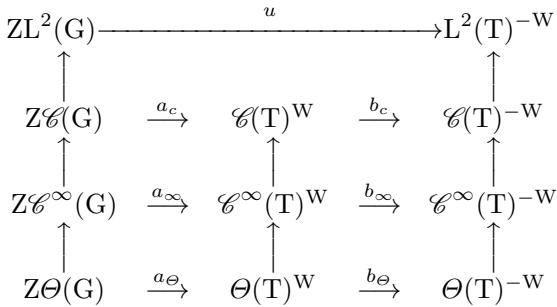
\includegraphics[keepaspectratio]{images/part003_8b0b3ceb.jpg}}

其中竖直箭头是典则包含映射，映射 \(b_{c}, b_{\infty}, b_{\Theta}\) 由 b 诱导，而 u 通过连续性延拓 \(b_{c} \circ a_{c}\)（§7, no. 4, Cor. 3 of Th. 2）。映射 u 和 \(b_{\Theta}\) 是双射（loc. cit.）；\(b_{\infty}\) 也是双射（Exerc. 5）；另一方面，\(b_{c}\) 一般不是满射（Exerc. 6）。

\section{紧李群在流形上的作用}

本节中，X 表示一个分离的、局部有限维的 \(C^{r}\) 类实流形（\(1 \leq r \leq \omega\)）。

\subsection{在紧集邻域中的流形嵌入}

引理 1. 设 T 和 T' 是两个拓扑空间，A 和 A' 分别是 T 和 T' 的紧子集，W 是 T × T' 中 A × A' 的一个邻域。存在 T 中 A 的开邻域 U 和 T' 中 A' 的开邻域 U'，使得 U × U' ⊂ W。

设 \(x \in \mathrm{A}\)；存在 \(\mathrm{U}_x\)（\(\mathrm{T}\) 的开子集）和 \(\mathrm{U}_x'\)（\(\mathrm{T}'\) 的开子集），使得 \(\{x\} \times \mathrm{A}' \subset \mathrm{U}_x \times \mathrm{U}_x' \subset \mathrm{W}\)：事实上，紧子集 \(\{x\} \times \mathrm{A}'\)（属于 \(\mathrm{T} \times \mathrm{T}'\)）可由有限个包含于 \(\mathrm{W}\) 中的开集覆盖，这些开集形如 \(\mathrm{U}_i \times \mathrm{U}_i'\)，且 \(x \in \mathrm{U}_i\)；只需取 \(\mathrm{U}_x = \bigcap_i \mathrm{U}_i\) 和 \(\mathrm{U}_x' = \bigcup_i \mathrm{U}_i'\) 即可。

由于 A 紧，存在 A 中的点 \(x_{1},\ldots,x_{m}\)，使得 \(A\subset\bigcup_{i}U_{x_{i}}\)；置 \(U=\bigcup_{i}U_{x_{i}}\) 和 \(U'=\bigcap_{i}U'_{x_{i}}\)。于是 \(A\times A'\subset U\times U'\subset W\)，引理得证。

本节余下部分中，Y 表示一个 \(C^{r}\) 类分离流形。

命题 1. 设 \(\varphi : \mathrm{X} \to \mathrm{Y}\) 是一个 \(\mathbf{C}^r\) 类态射，A 是 \(\mathrm{X}\) 的紧子集。下列条件等价：

\begin{enumerate}
\def\labelenumi{(\roman{enumi})}
\item
  \(\varphi\) 在 A 上的限制是单射，且 \(\varphi\) 在 A 的每一点处都是浸入；
\item
  存在 A 的一个开邻域 U，使得 \(\varphi\) 将 U 嵌入 Y 中。
\end{enumerate}

满足这些条件时，称 \(\varphi\) 在 A 的邻域中是嵌入。

证明 (i) 蕴含 (ii)，反向显然。假设 (i)，则存在包含 A 的 X 的一个开邻域 V，使得 \(\varphi\) 在 V 上是浸入（Differentiable and Analytic Manifolds, Results, 5.7.1）。记 \(\Gamma\) 为点 \((x,y)\)（属于 \(V \times V\)）且满足 \(\varphi(x) = \varphi(y)\) 的集合，记 \(\Delta\) 为 \(V \times V\) 中的对角线。则 \(\Delta\) 是 \(\Gamma\) 的开子集：事实上，对于所有 \(x \in V\)，存在 x 的一个开邻域 \(U_x\)，使得 \(\varphi\) 在 \(U_x\) 上是单射，即 \(\Gamma \cap (\mathrm{U}_x \times \mathrm{U}_x) = \Delta \cap (\mathrm{U}_x \times \mathrm{U}_x)\)。

由于 Y 是分离的，\(\varGamma\) 在 \(V \times V\) 中是闭的；因此 \(\varGamma - \varDelta\) 在 \(V \times V\) 中的补集 W 是开的。由假设，W 包含 \(A \times A\)；由引理 1，存在 V 中包含 A 的开子集 \(U'\)，使得 \(U' \times U' \subset W\)，也就是说，\(\varphi\) 在 \(U'\) 上的限制是单射。此外，存在 A 的一个开邻域 U，其闭包是紧的且包含于 \(U'\) 中（General Topology, Chap. I, §9, no. 7, Prop. 10）。于是 \(\varphi\) 诱导出从 \(\overline{U}\) 到 \(\varphi(\overline{U})\) 的同胚，因而也诱导出从 U 到 \(\varphi(U)\) 的同胚；由此 \(\varphi\) 在 U 上的限制是嵌入（Differentiable and Analytic Manifolds, Results, 5.8.3）。

命题 2. 假设流形 Y 是仿紧的；设 A 是 X 的子集，且 \(\varphi : X \to Y\) 是一个 \(C^r\) 类态射，它诱导出从 A 到 \(\varphi(A)\) 的同胚，并且在 A 的每一点处都是局部微分同胚。则存在 A 的一个开邻域 U，使得 \(\varphi\) 诱导出从 U 到 Y 的一个开子流形的同构。

必要时限制 X 和 Y 后，可假设 \(\varphi\) 是局部微分同胚且为满射。记 \(\sigma : \varphi(A) \to A\) 为 \(\varphi|A\) 的逆同胚。由于 Y 是可度量化的（Differentiable and Analytic Manifolds, Results, 5.1.6），\(\varphi(A)\) 有一个由仿紧邻域组成的基本邻域系；因此由 General Topology, Chap. XI，存在 Y 中 \(\varphi(A)\) 的一个开邻域 V 以及连续映射 \(s : V \to X\)，使得 s 与 \(\sigma\) 在 \(\varphi(A)\) 上一致，并且 \(\varphi(s(y)) = y\) 对所有 \(y \in V\) 成立。此外，s 在拓扑意义下是局部微分同胚的，故 \(s(V)\) 是包含 A 的开集 U。于是 \(\varphi\) 诱导出从 U 到 V 的同胚 \(\varphi'\)；由 Differentiable and Analytic Manifolds, Results, 5.7.8，\(\varphi'\) 是同构。

本节余下部分中，假设 \(r \neq \omega\)。

命题 3. 设 A 是 X 的紧子集。在 A 的邻域中为嵌入的态射 \(\varphi \in \mathcal{C}^{r}(X;Y)\) 所成的集合 P，在 \(\mathcal{C}^{r}(X;Y)\) 中关于紧 \(C^{r}\) 收敛的拓扑（\(\S\) 6, no. 4）下是开的。

显然，只需对 \(r = 1\) 证明该命题。

\begin{enumerate}
\def\labelenumi{\alph{enumi})}
\tightlist
\item
  先证明 \(\mathcal{C}^{1}(\mathrm{X};\mathrm{Y})\) 的子集 J 是开的，其中 J 由在 A 的每一点处为浸入的态射组成。考虑映射 \(j_{\mathrm{A}}:\mathcal{C}^{1}(\mathrm{X};\mathrm{Y})\times\mathrm{A}\to\mathrm{J}^{1}(\mathrm{X};\mathrm{Y})\)，满足 \(j_{\mathrm{A}}(\varphi,x)=j_{x}^{1}(\varphi)\)（Differentiable and Analytic Manifolds, Results, 12.1）。
\end{enumerate}

由 \(\mathcal{C}^1 (\mathrm{X};\mathrm{Y})\) 上拓扑的定义，映射 \(\tilde{j}_{\mathrm{A}}:\varphi \to j_{\mathrm{A}}(\varphi ,.)\) 从 \(\mathcal{C}^1 (\mathrm{X};\mathrm{Y})\) 到 \(\mathcal{C}(\mathrm{A};\mathrm{J}^1 (\mathrm{X};\mathrm{Y}))\) 是连续的；由此根据 General Topology, Chap. X, §3, no. 4, Th. 3，\(j_{\mathrm{A}}\) 是连续的。

另一方面，设 M 是 \(\mathrm{J}^{1}(\mathrm{X};\mathrm{Y})\) 中的喷流 j 的集合，这些喷流的切映射 \(\mathrm{T}(j):\mathrm{T}_{\mathbf{s}(j)}(\mathrm{X})\to\mathrm{T}_{\mathbf{b}(j)}(\mathrm{Y})\)（Differentiable and Analytic Manifolds, Results, 12.3.4）是单射。集合 M 在 \(\mathrm{J}^{1}(\mathrm{X};\mathrm{Y})\) 中是开的；事实上，只需在 X 是有限维向量空间 E 的开子集且 Y 是 Banach 空间 F 的开子集时验证该断言；根据 Differentiable and Analytic Manifolds, Results, 12.3.1，这归结为证明单射连续线性映射的集合在 \(\mathcal{L}(\mathrm{E};\mathrm{F})\) 中是开的，而这由 Spectral Theory, Chap. III, §2, no. 7, Prop. 16 得到。

由前述结果，集合 \(j_{\mathrm{A}}^{-1}(\mathrm{M})\) 在 \(\mathcal{C}^{1}(\mathrm{X};\mathrm{Y})\times\mathrm{A}\) 中是开的，故其补集 F 是闭的。由于 A 紧，投影 \(\mathrm{pr}_{1}:\mathcal{C}^{1}(\mathrm{X};\mathrm{Y})\times\mathrm{A}\to\mathcal{C}^{1}(\mathrm{X};\mathrm{Y})\) 是真的态射，因而是闭映射；所以集合 J（等于 \(\mathcal{C}^{1}(\mathrm{X};\mathrm{Y})-\mathrm{pr}_{1}(\mathcal{F})\)）在 \(\mathcal{C}^{1}(\mathrm{X};\mathrm{Y})\) 中是开的。

\begin{enumerate}
\def\labelenumi{\alph{enumi})}
\setcounter{enumi}{1}
\tightlist
\item
  设 H 是 \(J \times A \times A\) 的子集，由元素 \((f, x, y)\) 组成，满足 \(f(x) = f(y)\)。显然 H 包含 \(J \times \Delta\)，其中 \(\Delta\) 表示乘积 \(A \times A\) 中的对角线；我们证明 \(H' = H - (J \times \Delta)\) 在 \(J \times A \times A\) 中是闭的。由于 P 是 J 中 \(H'\) 在真的投影 \(pr_{1}: J \times A \times A \to J\) 下的像的补集，这将推出该命题。
\end{enumerate}

由于 \(\mathcal{C}^{1}(\mathrm{X};\mathrm{Y})\) 的拓扑比紧收敛拓扑精细，映射 \((\varphi,x)\mapsto\varphi(x)\) 从 \(\mathcal{C}^{1}(\mathrm{X};\mathrm{Y})\times\mathrm{A}\) 到 Y 是连续的（General Topology, Chap. X, §3, no. 4, Cor. 1 of Th. 3）；由此 H 在 \(J\times A\times A\) 中是闭的。因此只需证明 \(J\times\Delta\) 在 H 中是开的，换言之，对于所有 \(\varphi\in J\) 和所有 \(x\in A\)，存在一个邻域 \(\Omega\)（J 中 \(\varphi\) 的邻域）以及 X 中 x 的一个邻域 B，使得对于任意态射 \(\psi\)（属于 \(\Omega\)），\(\psi\) 在 \(A\cap B\) 上的限制是单射。

因此，该命题由下列引理推出：

引理 2. 设 x 是 X 的一点，\(\varphi: X \to Y\) 是一个 \(C^{1}\) 类态射，且在 x 处是浸入。存在一个邻域 \(\Omega\)（\(\varphi\) 在 \(\mathcal{C}^{1}(X;Y)\) 中的邻域）以及 X 中 x 的一个邻域 B，使得对于所有 \(\psi \in \Omega\)，\(\psi\) 在 B 上的限制是单射。

设 U 是 x 的一个相对紧开邻域，它同构于某个有限维向量空间，并且 \(\varphi(\overline{\mathrm{U}})\) 包含于图册的定义域 V 中。由集合 \(\Omega_{0}\)（它由满足 \(\psi\in\mathcal{C}^{1}(\mathrm{X};\mathrm{Y})\) 且 \(\psi(\overline{\mathrm{U}})\subset\mathrm{V}\) 的态射组成）在 \(\mathcal{C}^{1}(\mathrm{X};\mathrm{Y})\) 中是开的，且限制映射 \(\Omega_{0}\to\mathcal{C}^{1}(\mathrm{U};\mathrm{V})\) 是连续的；因此只需在 X=U 且 Y=V 时证明该引理，换言之，可假设 X 是有限维向量空间而 Y 是 Banach 空间。在 X 和 Y 上选取范数。

线性映射 \(\mathrm{D}\varphi(x):\mathrm{X}\to\mathrm{Y}\) 是单射；记其余范数为 q（Spectral Theory, Chap. III, §2, no. 6），于是按定义，有 \(\|\mathrm{D}\varphi(x).t\|\geq q\|t\|\) 对所有 \(t\in X\) 成立。取 \(\varepsilon\in R\) 使得 \(0<\varepsilon<q/2\)，并取一个以 x 为中心的闭球 B，使得 \(\|\mathrm{D}\varphi(u)-\mathrm{D}\varphi(x)\|\leq\varepsilon\) 对所有 \(u\in B\) 成立。记 \(\Omega\) 为 \(\mathcal{C}^{1}(\mathrm{X};\mathrm{Y})\) 中的态射 \(\psi\) 所成的子集，其中满足 \(\|\mathrm{D}\psi(u)-\mathrm{D}\varphi(u)\|\leq\varepsilon\) 对所有 \(u\in B\) 成立；按 \(\mathcal{C}^{1}(\mathrm{X};\mathrm{Y})\) 拓扑的定义，它是开的。对于 \(\psi\in\Omega\)，置 \(\psi_{0}=\psi-\mathrm{D}\varphi(x)\)。有 \(\|\mathrm{D}\psi_{0}(u)\|\leq2\varepsilon\) 对所有 \(u\in B\) 成立，因而有 \(\|\psi_{0}(u)-\psi_{0}(v)\|\leq2\varepsilon\|u-v\|\) 对 B 中所有 u 和 v 成立（Differentiable and Analytic Manifolds, Results, 2.2.3）。由此

\[
\| \psi (u) - \psi (v) \| \geq \| \mathrm{D} \varphi (x). (u - v) \| - \| \psi_ {0} (u) - \psi_ {0} (v) \| \geq (q - 2 \varepsilon) \| u - v \|.
\]

所以 \(\psi\) 在 B 上的限制是单射，引理得证。

命题 4. 设 A 是 X 的紧子集。存在有限维向量空间 E 以及一个态射 \(\varphi \in \mathcal{C}^r (\mathrm{X};\mathrm{E})\)（\(r\neq \omega\)），使得它在 A 的邻域中是嵌入。

设 \((\mathrm{U}_{i},\varphi_{i},\mathrm{E}_{i})_{i\in\mathrm{I}}\) 是 X 的一个有限图册族，其定义域覆盖 A。我们将 \(\varphi_{i}\) 延拓为从 X 到 \(E_{i}\) 的映射（仍记作 \(\varphi_{i}\)），规定 \(\varphi_{i}(x)=0\)（\(x\notin U_{i}\)）。设 \((\mathrm{V}_{i})_{i\in\mathrm{I}}\) 是由 X 的开子集组成的 A 的一个覆盖，使得 \(\overline{\mathrm{V}}_{i}\subset\mathrm{U}_{i}\) 对所有 \(i\in\mathrm{I}\) 成立（这种覆盖的存在性由 General Topology, Chap. IX, §4, no. 3, Cor. 1 of Th. 3 得到：将该结果应用于紧空间 \(X'\) 及 \(X'\) 的覆盖，后者由开集 \(U_{i}\)（\(i\in\mathrm{I}\)）和 \(X'-\mathrm{A}\) 组成；X' 是通过向 X 添加无穷远点得到的空间）。对于所有 \(i\in\mathrm{I}\)，取 \(\alpha_{i}\) 为 X 上的一个 \(C^{r}\) 类数值函数，它在 \(V_{i}\) 的每一点处等于 1，且其支集包含于 \(U_{i}\)（Differentiable and Analytic Manifolds, Results, 5.3.6）。

考虑由下式定义的映射 \(\varphi : \mathrm{X} \to \bigoplus_{i \in \mathrm{I}} (\mathrm{E}_i \oplus \mathbf{R})\)

\[
\varphi (x) = (\alpha_ {i} (x) \varphi_ {i} (x), \alpha_ {i} (x)) _ {i \in I}.
\]

对于所有 \(i \in I\)，映射 \(\alpha_{i}\varphi_{i}\) 是 \(C^{r}\) 类的（因为它在 \(U_{i}\) 以及 \(\alpha_{i}\) 的支集的补集上的限制都是如此），且其在 \(V_{i}\) 上的限制是嵌入；由此 \(\varphi\) 是 \(C^{r}\) 类态射，并且在 A 的每一点处都是浸入。我们证明 \(\varphi\) 在 A 上的限制是单射。设 x、y 是 A 中满足 \(\varphi(x) = \varphi(y)\) 的两点，并取 \(i \in I\)，使得 \(x \in V_{i}\)。则 \(\alpha_{i}(x) = 1\)，所以 \(\alpha_{i}(y) = 1\)，这推出 \(y \in U_{i}\)；但还有 \(\varphi_{i}(x) = \varphi_{i}(y)\)，故 x = y，因为 \(\varphi_{i}\) 将 \(U_{i}\) 嵌入 \(E_{i}\)。

可以证明 \(^{9}\)，每个分离的、无穷远可数且纯维数为 n 的流形都能嵌入 \(R^{2n}\)；较弱的结果见 cf.~Exercise 2。

\subsection{等变嵌入定理}

本节中假设 \(r \neq \omega\)。

引理 3. 设 G 是一个在拓扑空间 X 上连续作用的紧拓扑群；设 A 是 X 的子集，在 G 的作用下稳定，W 是 A 的一个邻域。则存在 A 的一个开邻域 V，在 G 的作用下稳定且包含于 W 中。

置 \(\mathrm{F} = \mathrm{X} - \mathrm{W}\) 和 \(\mathrm{V} = \mathrm{X} - \mathrm{GF}\)。则 \(\mathrm{V}\) 是开的（General Topology, Chap. III, §4, no. 1, Cor. 1 of Prop. 1），在 \(\mathrm{G}\) 的作用下稳定，且 \(\mathrm{A} \subset \mathrm{V} \subset \mathrm{W}\)。

定理 1. 设 G 是紧李群，\((g,x)\mapsto gx\) 是 G 在 X 上的 \(C^{r}\) 类左作用律，A 是 X 的紧子集。存在 G 在有限维向量空间 E 上的解析线性表示 \(\rho\)、一个态射 \(\varphi:X\to E\)（为 \(C^{r}\) 类，与 G 的作用相容）以及 A 的一个开邻域 U，在 G 的作用下稳定，使得 \(\varphi\) 在 U 上的限制是嵌入。

用紧集 GA 替换 A 后，可归结为 A 在 G 的作用下稳定的情形。

设 \(E_0\) 是一个有限维向量空间，使得 \(\mathcal{C}^r(\mathrm{X};\mathrm{E}_0)\) 中存在在 A 的邻域中为嵌入的元素（no. 1, Prop. 4）；具有此性质的态射所成的集合 \(\mathcal{P}\) 是 \(\mathcal{C}^r(\mathrm{X};\mathrm{E}_0)\) 的非空开子集（no. 1, Prop. 3）。考虑紧群 G 在空间 \(\mathcal{C}^r(\mathrm{X};\mathrm{E}_0)\) 上的连续线性表示（§6, no. 4, Lemma 4）。由 Peter–Weyl 定理（Spectral Theory, in preparation），在 G 的作用下稳定的有限维子空间之并在 \(\mathcal{C}^r(\mathrm{X};\mathrm{E}_0)\) 中稠密；因此，存在元素 \(\varphi_0\) 属于 \(\mathcal{P}\)，使得映射 \(x \mapsto \varphi_0(gx)\)（\(g \in G\)）生成有限维向量子空间 \(E_1\)，它是 \(\mathcal{C}^r(\mathrm{X};\mathrm{E}_0)\) 的子空间，该子空间显然在 G 的作用下稳定。

取 E 为空间 \(\operatorname{Hom}_{\mathbf{R}}(\mathrm{E}_{1},\mathrm{E}_{0})\)，取 \(\rho\) 为 G 在 E 上由其在 \(E_{1}\) 上的作用诱导的表示，并令 \(\varphi:X\to E\) 为将 \(x\in X\) 赋予线性映射 \(\psi\mapsto\psi(x)\)（从 \(E_{1}\) 到 \(E_{0}\)）的映射。这是 \(C^{r}\) 类态射；对于 \(x\in X\)、\(g\in G\)、\(\psi\in E_{1}\)，有（记 \(\tau(g)\) 为 X 的自同构 \(x\mapsto gx\)）：

\[
\varphi (g x) (\psi) - \psi (g x) = \varphi (x) (\psi \circ \tau (g)) = (\rho (g) \varphi (x)) (\psi).
\]

令 \(\alpha : \mathrm{Hom}_{\mathbf{R}}(\mathrm{E}_1, \mathrm{E}_0) \to \mathrm{E}_0\) 为线性映射 \(u \mapsto u(\varphi_0)\)；有 \(\alpha \circ \varphi = \varphi_0\)，所以 \(\varphi\) 在 A 的邻域中是嵌入（因为 \(\varphi_0\) 是嵌入）。因此存在 A 的一个开邻域 U，使得 \(\varphi\) 在 U 上的限制是嵌入；由引理 3 可将 U 选为在 G 的作用下稳定的，定理得证。

推论 1. 假设 X 是紧的。存在 G 在有限维向量空间 E 上的解析线性表示 \(\rho\) 以及一个嵌入 \(\varphi: X \to E\)，使得 \(\varphi(gx) = \rho(g)\varphi(x)\) 对 \(g \in G, x \in X\) 成立。

推论 2. 设 H 是 G 的闭子群。存在 G 在有限维向量空间 E 上的解析线性表示以及一点 \(v \in E\)，其固定子群为 H。

将推论 1 应用于 G 在紧流形 G/H 上的典则作用。这给出解析线性表示 \(\rho: \mathrm{G} \to \mathbf{GL}(\mathrm{E})\) 以及嵌入 \(\varphi: \mathrm{G} / \mathrm{H} \to \mathrm{E}\)，使得 \(\varphi(gx) = \rho(g)\varphi(x)\)，其中 \(g \in \mathrm{G}, x \in \mathrm{G} / \mathrm{H}\)。令 \(\bar{e} \in \mathrm{G} / \mathrm{H}\) 为 \(e \in \mathrm{G}\) 的等价类，并令 \(v = \varphi(\bar{e})\) 为其像。对于所有 \(g \in \mathrm{G}\)，有 \(\rho(g)v = v \Longleftrightarrow \varphi(g\bar{e}) = \varphi(\bar{e}) \Longleftrightarrow g\bar{e} = \bar{e} \Longleftrightarrow g \in \mathrm{H}\)。

推论 3. 假设 X 是仿紧的。存在实希尔伯特空间 E、G 在 E 上的连续酉表示 \({}^{10}\) \(\rho\) 以及一个嵌入 \(\varphi: X \to E\)（为 \(C^{r}\) 类），使得 \(\varphi(gx) = \rho(g)\varphi(x)\) 对所有 \(g \in G\) 和所有 \(x \in X\) 成立。

空间 X/G 是局部紧的（General Topology, Chap. III, §4, no. 5, Prop. 11）。它的连通分支是 X 的连通分支的像，而 X 的连通分支在无穷远处可数（General Topology, Chap. I, §9, no. 10, Th. 5）；因此这些像自身也在无穷远处可数，从而 X/G 是仿紧的（loc. cit.）。所以存在 X/G 的一个局部有限覆盖 \((\mathrm{U}_{\alpha}^{\prime})_{\alpha\in\mathrm{I}}\)，其成员为相对紧开集；还存在覆盖 \((\mathrm{V}_{\alpha}^{\prime})_{\alpha\in\mathrm{I}}\)，使得 \(\overline{V}_{\alpha}^{\prime}\subset U_{\alpha}^{\prime}\) 对所有 \(\alpha\in I\) 成立（General Topology, Chap. IX, §4, no. 3, Cor. 1 of Th. 3）。取逆像后，得到 X 的两个局部有限覆盖 \((\mathrm{U}_{\alpha})_{\alpha\in\mathrm{I}}\) 和 \((\mathrm{V}_{\alpha})_{\alpha\in\mathrm{I}}\)，其成员为在 G 下稳定的相对紧开集，并且 \(\overline{V}_{\alpha}\subset U_{\alpha}\) 对所有 \(\alpha\in I\) 成立。

对于所有 \(\alpha \in \mathrm{I}\)，存在一个表示 \(\rho_{\alpha}\)，它作用在有限维实向量空间 \(\mathrm{E}_{\alpha}\) 上，以及一个与 G 的作用相容的态射 \(\varphi_{\alpha} \in \mathcal{C}^r (\mathrm{X};\mathrm{E}_{\alpha})\)，且其在 \(\mathrm{U}_{\alpha}\) 上的限制是嵌入（定理 1）。对于 \(\alpha \in \mathrm{I}\)，取一个 \(a_{\alpha}\)，它是 X 上的 \(\mathrm{C}^r\) 类数值函数，在 \(\mathrm{V}_{\alpha}\) 上等于 1，在 \(\mathrm{U}_{\alpha}\) 外等于 0（Differentiable and Analytic Manifolds, Results, 5.3.6）。置 \(b_{\alpha}(x) = \int_{\mathrm{G}} a_{\alpha}(gx) dg\) 对于 \(x \in \mathrm{X}\) 成立。函数 \(b_{\alpha}\) 是 \(\mathrm{C}^r\) 类的，在 G 下不变（§6, no. 4, Cor. 2），在 \(\mathrm{V}_{\alpha}\) 上等于 1，在 \(\mathrm{U}_{\alpha}\) 外等于 0。在每个 \(\mathrm{E}_{\alpha}\) 上取一个 G-不变的希尔伯特内积（§1, no. 1），并在 R 上取其典则希尔伯特结构；令 E 为族 \((\mathrm{E}_{\alpha} \oplus \mathbf{R})_{\alpha \in \mathrm{I}}\) 的希尔伯特和，并令 \(\rho\) 为 G 在 E 上由各 \(\rho_{\alpha}\) 以及 G 在 R 上的平凡作用诱导的表示。对于 \(x \in \mathrm{X}\)，置 \(\varphi(x) = (b_{\alpha}(x)\varphi_{\alpha}(x), b_{\alpha}(x))_{\alpha \in \mathrm{I}}\)。则 \(\varphi\) 是从 X 到 E 的 \(\mathrm{C}^r\) 类态射，与 G 的作用相容；如命题 4 的证明（no. 1）中那样验证 \(\varphi\) 是嵌入，即得该推论。

\subsection{管与横截面}

引理 4. 设 H 是紧李群，\(\rho : \mathrm{H} \to \mathbf{GL}(\mathrm{V})\) 是 H 在有限维实向量空间 V 上的连续（因而解析）表示，W 是 V 中原点的一个邻域。存在原点的一个开邻域 B，它包含于 W 且在 H 的作用下稳定；还存在一个解析同构 \(u: \mathrm{V} \to \mathrm{B}\)，与 H 的作用相容，并满足 \(u(0) = 0\) 和 \(\mathrm{Du}(0) = \mathrm{Id}_{\mathrm{V}}\)。

在 V 上选取一个 H-不变内积（§1, no. 1）。存在实数 \(r > 0\)，使得半径为 \(r\) 的开球 B 包含于 W 中；它显然在 H 的作用下稳定。置 \(u(v) = r(r^2 + \|v\|^2)^{-1/2} v\)，对所有 \(v \in V\) 成立；于是 \(u\) 是从 V 到 B 的双射解析映射，与 H 的作用相容，且其逆映射 \(w \mapsto r(r^2 - \|w\|^2)^{-1/2} w\) 是解析的。此外，\(u(0) = 0\) 且 \(\mathrm{D}u(0) = \mathrm{Id}_{\mathrm{V}}\)。

命题 5. 设 H 是紧李群，\((h,x)\mapsto hx\) 是 H 在 X 上的 \(C^{r}\) 类左作用律，x 是 X 中在 H 的作用下固定的一点。则群 H 在线性地作用于向量空间 \(T=T_{x}(X)\) 上；存在一个开嵌入 \(\varphi:T\to X\)，为 \(C^{r}\) 类，与 H 的作用相容，并满足 \(\varphi(0)=x\) 且 \(T_{0}(\varphi)\) 是 T 的恒等映射。

设 \((\mathrm{U},\psi,\mathrm{E})\) 是 X 在 x 处的一个图册，使得 U 在 H 的作用下稳定（no. 2, Lemma 3）且 \(\psi(x)=0\)。通过 \(\mathrm{T}_{x}(\psi)\) 将 E 与 T 识别，并置

\[
\psi^ {\sharp} (y) = \int_ {\mathrm{H}} h. \psi (h ^ {- 1} y) d h \quad \text { for } y \in \mathrm{U},
\]

其中 dh 是 H 上总质量为 1 的 Haar 测度。

于是（§6, no. 4, Cor. 1）\(\psi^{\sharp}\) 是从 U 到 T 的 \(\mathrm{C}^r\) 类态射，与 H 的作用相容，并满足 \(\psi^{\sharp}(x) = 0\) 和 \(d_x\psi^\sharp = \mathrm{Id}_\mathrm{T}\)。因此存在一个开集 \(\mathrm{U}' \subset \mathrm{U}\)，包含 \(x\)，以及 T 中 0 的一个开邻域 V，使得 \(\psi^{\sharp}\) 诱导出同构 \(\theta: \mathrm{U}' \to \mathrm{V}\)。必要时限制 \(\mathrm{U}'\) 和 V，可假设它们在 H 的作用下稳定，并且存在与 H 的作用相容的同构 \(u: \mathrm{T} \to \mathrm{V}\)（引理 4）。现在只需取 \(\varphi = \theta^{-1} \circ u\)。

回忆（Differentiable and Analytic Manifolds, Results, 6.5.1），若 G 是李群，H 是 G 的李子群，且 Y 是 H 在其上左作用的流形，则记 \(G \times^{H}Y\) 为乘积流形 \(G \times Y\) 关于 H 的右作用 \(((g,y),h) \mapsto (gh,h^{-1}y)\) 的商；这是一个李群 G 在其上自然地左作用的流形；投影 \(G \times^{H}Y \to G/H\) 是纤维为 Y 的丛。此外，若 Y 是 H 在线性作用的有限维向量空间，则 \(G \times^{H}Y\) 自然具有以 G/H 为底空间的向量 G-丛结构（Differentiable and Analytic Manifolds, Results, 7.10.2）。

设 G 是一个在流形 X 上真作用的李群（General Topology, Chap. III, §4, no. 1, Def. 1），且作用律 \((g, x) \mapsto gx\) 是 \(C^{r}\) 类的。则对于 X 中的每一点 x，x 的轨道 Gx 是 X 的闭子流形，同构于李齐性空间 \(G/G_{x}\)，其中 \(G_{x}\) 是 G 中 x 的固定子群（cf.~Chap. III, §1, no. 7, Prop. 14 (ii), and General Topology, Chap. III, §4, no. 2, Prop. 4）；后者是紧李群（loc. cit.）。

命题 6. 假设流形 X 是仿紧的；设 x 是 X 中的一点，\(G_{x}\) 是其固定子群。存在有限维解析线性表示 \(\tau: G_{x} \to \mathbf{GL}(W)\)，以及一个开嵌入 \(\alpha: G \times ^{G_{x}} W \to X\)，为 \(C^{r}\) 类，与 G 的作用相容，并将 \((e,0) \in G \times W\) 的等价类映到 x。

置 \(T = T_{x}(X)\)。设 W 是 T 中 \(T_{x}(Gx)\) 的一个补子空间，在 \(G_{x}\) 的作用下稳定（例如，取 \(T_{x}(Gx)\) 相对于 T 上 \(G_{x}\)-不变内积的正交补）。另一方面，设 \(\varphi : T \to X\) 是具有命题 5 所述性质的态射（相对于 \(H = G_{x}\)）。考虑态射 \(\lambda : G \times W \to X\)，其定义为 \(\lambda(g, w) = g\varphi(w)\)。它通过取商诱导出态射 \(\mu : G \times^{G_{x}}W \to X\)，为 \(C^{r}\) 类，与 G 的作用相容，并将 \((e, 0)\) 的等价类 z 映到 x。

我们证明 \(\mu\) 在点 \(z\) 处是局部微分同胚的。有

\[
\begin{array}{c} \dim (\mathrm{G} \times {} ^ {\mathrm{G} _ {x}} \mathrm{W}) = \dim (\mathrm{G}) + \dim (\mathrm{W}) - \dim (\mathrm{G} _ {x}) \\ = \dim (\mathrm{G} x) + \dim (\mathrm{W}) = \dim (\mathrm{T}), \end{array}
\]

所以只需证明 \(\mu\) 在 \(z\) 处是下沉映射，或等价地，\(\lambda\) 在 \((e,0)\) 处是下沉映射。但是，切映射 \(\mathrm{T}_{(e,0)}(\lambda):\mathrm{T}_e(\mathrm{G})\oplus \mathrm{W}\to \mathrm{T}\) 等于 \(\mathrm{T}_e(\rho (x)) + i\)，其中 \(\rho (x)\) 是轨道映射 \(g\mapsto gx\)，而 \(i\) 是从 W 到 T 的典则嵌入；由于 \(\operatorname {Im}\operatorname {T}_e(\rho (x)) = \operatorname {T}_x(\operatorname {G}x)\)，切映射 \(\mathrm{T}_{(e,0)}(\lambda)\) 是满射，且 \(\mu\) 在 \(z\) 处是局部微分同胚的。

我们将证明，存在一个开邻域 \(\Omega\)，它是 \(Gz\) 在 \(G \times ^{G_x}W\) 中的邻域，在 \(G\) 的作用下稳定，使得 \(\mu\) 将 \(\Omega\) 同构到 \(X\) 的一个开子集上。这将推出该命题：事实上，\(\Omega\) 在 \(G \times W\) 中的逆像在 \(G\) 的作用下稳定，因而形如 \(G \times B\)，其中 \(B\) 是 \(W\) 中包含原点且在 \(G_x\) 的作用下稳定的开子集；必要时限制 \(\Omega\)，可假设存在同构 \(u: W \to B\)，与 \(G_x\) 的作用相容（引理 4）。显然，复合态射 \(\alpha: G \times ^{G_x}W \xrightarrow{(\text{Id}, u)} G \times ^{G_x}B \xrightarrow{\mu} X\) 满足命题中的条件。

因此，该命题是下列引理的推论：

引理 5. 设 Z 是一个 \(C^{r}\) 类分离流形，带有一个左作用律 \(m: G \times Z \to Z\)，为 \(C^{r}\) 类，且 \(\mu: Z \to X\) 是一个与 G 的作用相容的（\(C^{r}\) 类）态射。设 z 是 Z 中的一点，且 \(x = \mu(z)\)。假设 \(\mu\) 在 z 处是局部微分同胚的，且 G 中 z 的固定子群等于 x 的固定子群 \(G_{x}\)。则存在一个开邻域 \(\Omega\)，它是轨道 Gz 的邻域，在 G 的作用下稳定，使得 \(\mu\) 将 \(\Omega\) 同构到 X 的一个开子集上。

由于 \(\mu\) 与 G 的作用相容，它在 Gz 的每一点处都是局部微分同胚的；由于典则映射 \(G/G_{x} \rightarrow Gx\) 是同胚，由 \(\mu\) 诱导的从 Gz 到 Gx 的映射也是同胚。因此由 no. 1 的命题 2 可知，Z 中存在 Gz 的一个开邻域 U，使得 \(\mu\) 将 U 开嵌入 X。

由于 G 在 X 上真作用，存在 x 的一个开邻域 V 以及 G 的一个紧子集 K，使得当 \(gV \cap V = \varnothing\)（\(g \notin K\) 时）；特别地，\(e \in K\)。集合 \(W_{1}\) 由 Z 中满足 \(y \in Z\) 且 \(Ky \subset U\) 的点组成，是开的：事实上，\(Z - W_{1}\) 是闭集 \((\mathrm{K} \times \mathrm{Z}) - m^{-1}(\mathrm{U})\) 在真投影 \(pr_{2}: K \times Z \to Z\) 下的像。置 \(W = W_{1} \cap \mu^{-1}(V)\)；这是 Z 的一个包含 z 的开子集，并满足下列条件：

\begin{enumerate}
\def\labelenumi{(\roman{enumi})}
\item
  KW \(\subset\) U，特别是 W \(\subset\) U；
\item
  \(\mu(\mathrm{W}) \subset \mathrm{V}.\)
\end{enumerate}

置 \(\Omega = \mathrm{GW}\)，并考虑 \(\mu\) 在 \(\Omega\) 上的限制。这是一个局部微分同胚态射，因为 \(\Omega\) 的每一点都在 \(\mathbf{G}\) 的作用下与 \(\mathbf{U}\) 中的一点共轭。我们证明它是单射：设 \(g, h\) 属于 \(\mathbf{G}\)，\(u, v\) 属于 \(\mathbf{W}\)，且满足 \(\mu(gu) = \mu(hv)\)。置 \(k = g^{-1}h\)；则 \(\mu(u) = k\mu(v)\)，由 (ii) 得 \(k \in \mathbf{K}\)。但由 (i)，\(kv\) 和 \(u\) 都属于 \(\mathbf{U}\)；于是 \(u = kv\)，因为 \(\mu\) 在 \(\mathbf{V}\) 上的限制是单射，所以 \(gu = hv\)。因此 \(\mu\) 在 \(\Omega\) 上的限制是单射，从而根据 Differentiable and Analytic Manifolds, Results, 5.7.8，它是到 \(\mathbf{X}\) 的一个开子流形上的同构，证明完成。

在命题 6 的条件下，\(\alpha\) 的像是轨道 A 的点 \(x\) 的一个开邻域 T，它带有以 A 为底空间的向量丛结构，且零截面就是轨道 A 本身。对于每个点 \(a \in \mathrm{A}\)，该向量丛的纤维 \(\mathrm{Y}_a\) 是 X 的子流形，在固定子群 \(\mathrm{G}_a\)（对应点 \(a\)）的作用下稳定，并且有一个从 \(\mathrm{G} \times^{\mathrm{G}_a}\mathrm{Y}_a\) 到 X 的态射，它将 \((g,y) \in \mathrm{G} \times \mathrm{Y}_a\) 的等价类映到 \(gy \in \mathrm{X}\)，并且它诱导出一个 \(\mathrm{C}^r\) 类态射，从 \(\mathrm{G} \times^{\mathrm{G}_a}\mathrm{Y}_a\) 到 T。称 \(\mathrm{Y}_a\) 为管 T 在 \(a\) 处的横截面。注意，在 \(a\) 处，\(\mathrm{Y}_a\) 的切空间典则同构于 \(\mathrm{Y}_a\)，并且它是 \(\mathrm{T}_a(\mathrm{A})\) 在 \(\mathrm{T}_a(\mathrm{X})\) 中的一个补空间；因此，以 A 为底空间的向量丛 T 典则同构于 A 在 X 中的法丛（Differentiable and Analytic Manifolds, Results, 8.1.3）。

\subsection{轨道类型}

设 \(G\) 是在分离拓扑空间 \(E\) 上连续作用的拓扑群。对于每一点 \(x\)（属于 \(E\)），记 \(G_x\) 为 \(x\) 在 \(G\) 中的固定子群，并假设典则映射 \(G / G_x \to Gx\) 是同胚；以下两种情形尤其满足此条件：

\begin{enumerate}
\def\labelenumi{\alph{enumi})}
\item
  G 和 E 的拓扑都是离散的；
\item
  G 在 E 上真作用（General Topology, Chap. III, §4, no. 2, Prop. 4），例如 G 是紧的（General Topology, Chap. III, §4, no. 1, Prop. 2）。
\end{enumerate}

记 \(\mathcal{T}\) 为 G 的闭子群的共轭类集合。对于每个 \(x\in \mathrm{E}\)，称 \(x\) 的轨道类型（有时简称 \(x\) 的类型）为 \(\mathrm{G}_x\) 在 \(\mathcal{T}\) 中的类；同一轨道上的两点具有相同的轨道类型（Algebra, Chap. I, §5, no. 2, Prop. 2）；两个轨道具有相同类型，当且仅当它们作为 G-集合同构（Algebra, Chap. I, §5, no. 5, Th. 1）。对于每个 \(t\in \mathcal{T}\)，记 \(\mathrm{E}_{(t)}\) 为 E 中类型为 \(t\) 的点的集合，即类型为 \(t\) 的轨道之并；这是 E 的稳定子集。对于 \(\mathrm{H}\in t\)，也将 \(\mathrm{E}_{(\mathrm{H})}\) 记作 \(\mathrm{E}_{(t)}\)；例如，\(\mathrm{E}_{(\mathrm{G})}\) 是由 G 固定的点组成的 E 的闭子空间。

在 T 上定义如下预序关系：

\(t \leq t'\Longleftrightarrow\) 存在 \(\mathrm{H} \in t\) 和 \(\mathrm{H}' \in t'\)，使得 \(\mathrm{H} \supset \mathrm{H}'\)。

设 \(\Omega\) 和 \(\Omega'\) 是 G 在 E 上的两个轨道，\(t\) 和 \(t'\) 分别是它们的类型；则 \(t \leq t'\) 当且仅当存在从 \(\Omega'\) 到 \(\Omega\) 的 G-态射（必为满射且连续）。

设 \(x, x'\) 属于 E，\(t, t'\) 是它们的类型；则 \(t \leq t'\) 当且仅当存在 \(a \in G\)，使得 \(aG_{x'}a^{-1} \subset G_x\)。

引理 6. 设 G 是李群。

\begin{enumerate}
\def\labelenumi{\alph{enumi})}
\item
  \(\mathbf{G}\) 的每个递降紧子群序列都是最终稳定的。
\item
  设 H 和 \(H'\) 是 G 的两个紧子群，满足 \(H \subset H'\)，且存在从 \(H'\) 到 H 的（拓扑群）同构。则 \(H = H'\)。
\item
  对于关系 \(t \leq t'\)，集合 \(\mathcal{T}\) 是一个诺特有序集（Theory of Sets, Chap. III, §6, no. 5, text preceding Prop. 7）。
\item
  设 \((\mathrm{H}_{i})_{i\geq1}\) 是 G 的一个递降紧子群序列；这些子群都是 G 的李子群（Chap. III, §8, no. 2, Th. 2）。整数序列 \((\dim\mathrm{H}_{i})_{i\geq1}\) 递降，因而最终稳定，所以存在整数 N，使得子群 \(H_{i}\) 在 \(i\geq N\) 时具有相同的单位元连通分支。于是正整数序列 \((\mathrm{H}_{i}:(\mathrm{H}_{i})_{0})_{i\geq N}\) 递降且最终稳定，因此当 i 充分大时 \(H_{i}=H_{i+1}\)。
\item
  设 \(f\) 是从 \(\mathrm{H}'\) 到 \(\mathrm{H}\) 的同构。序列 \((f^n(\mathrm{H}))_{n\geq 0}\) 是 \(\mathrm{G}\) 的递降紧子群序列，故 \(f^n(\mathrm{H}) = f^{n + 1}(\mathrm{H})\) 对充分大的 \(n\) 成立，由 \(a\) 可知。由于 \(f\) 是同构，这推出 \(f(\mathrm{H}) = \mathrm{H} = f(\mathrm{H}')\)，所以 \(\mathrm{H} = \mathrm{H}'\)。
\item
  设 \(t, t' \in \mathcal{T}\) 满足 \(t \leq t'\) 且 \(t' \leq t\)。则存在 \(\mathrm{H}, \mathrm{H}_1 \in t\) 和 \(\mathrm{H}', \mathrm{H}_1' \in t'\)，使得 \(\mathrm{H} \supset \mathrm{H}'\) 且 \(\mathrm{H}_1 \subset \mathrm{H}_1'\)。设 \(g\) 和 \(g'\) 是 \(G\) 中满足 \(\mathrm{H}_1 = g\mathrm{H}g^{-1}\) 和 \(\mathrm{H}_1' = g'\mathrm{H}'g'^{-1}\) 的两个元素；置 \(u = g'^{-1}g\)。则
\end{enumerate}

\[
u \mathrm{H} u ^ {- 1} \subset \mathrm{H} ^ {\prime} \subset \mathrm{H};
\]

由 \(b\)，这推出 \(u\mathrm{H}u^{-1} = \mathrm{H}\)，所以 \(\mathrm{H}' = \mathrm{H}\) 且 \(t' = t\)。因此，集合 \(\mathcal{T}\) 是有序的，并由 \(a\) 可知它是诺特的。

定理 2. 设 \(\mathbf{G}\) 是在 \(\mathbf{X}\) 上真作用的李群，且作用律 \((g,x)\mapsto gx\) 是 \(\mathbf{C}^r\) 类的。假设 \(\mathbf{X}\) 是仿紧的。

\begin{enumerate}
\def\labelenumi{\alph{enumi})}
\item
  将 X 的每一点赋予其轨道类型的映射具有如下半连续性：设 \(x \in X\)，且 \(t \in T\) 是其轨道类型；存在 x 的一个稳定开邻域 U，使得对于任意 \(u \in U\)，u 的类型满足 \(\geq t\)。
\item
  对于所有 \(t \in \mathcal{T}\)，\(\mathrm{X}_{(t)}\) 是 \(\mathrm{X}\) 的子流形，\(\mathrm{X}_{(t)}\) 上由 \(\mathrm{G}\) 的作用诱导的等价关系是正则的（Differentiable and Analytic Manifolds, Results, 5.9.5），且态射 \(\mathrm{X}_{(t)} \to \mathrm{X}_{(t)} / \mathrm{G}\) 是一个丛。
\item
  假设 X/G 是连通的。则 X 中元素的轨道类型集合有最大元 \(\tau\)；此外，\(\mathrm{X}_{(\tau)}\) 是 X 的稠密开子集，且 \(\mathrm{X}_{(\tau)}/\mathrm{G}\) 是连通的。
\end{enumerate}

设 \(x\) 是 \(\mathrm{X}\) 中的一点，且 \(t \in \mathcal{T}\) 是其类型。为证明 \(a)\) 和 \(b)\)，可以将 \(\mathrm{X}\) 替换为包含 \(x\) 的稳定开集，从而（由命题 6）可假设 \(\mathrm{X}\) 形如 \(\mathrm{G} \times^{\mathrm{H}}\mathrm{W}\)，其中 \(\mathrm{W}\) 是紧子群 \(\mathrm{H}\)（属于 \(\mathrm{G}\)）的有限维解析线性表示空间，点 \(x\) 是典则投影 \(p(e,0)\) 的像，其中 \((e,0) \in \mathrm{G} \times \mathrm{W}\)，该典则投影为 \(p: \mathrm{G} \times \mathrm{W} \to \mathrm{G} \times^{\mathrm{H}}\mathrm{W}\)。若 \(u = p(g,y) \in \mathrm{G} \times^{\mathrm{H}}\mathrm{W}\) 且 \(a \in \mathrm{G}\)，则 \(au = u\) 当且仅当存在 \(h \in \mathrm{H}\)，使得 \((ag,y) = (gh^{-1},hy)\)，也就是 \(a \in g\mathrm{H}_yg^{-1}\)。因此，\(\mathrm{G}_u = g\mathrm{H}_yg^{-1}\)；特别地，\(\mathrm{G}_x = \mathrm{H}\)，所以 \(\mathrm{G}_u\) 与 \(\mathrm{G}_x\) 的一个子群共轭，这证明了 \(u\) 的类型 \(\geq t\)，从而得到 \(a)\)。

此外，u 的类型为 t，当且仅当 \(G_{u}\) 在 G 中与 H 共轭，或等价地，当且仅当 \(H_{y}\) 在 G 中与 H 共轭；由引理 6 b)，这意味着 \(H_{y} = H\)，从而 y 被 H 固定。若 \(W'\) 是 W 中由 H 固定的元素组成的向量子空间，则 \(\mathrm{X}_{(t)}\) 可与 \(G \times {}^{H}W'\) 识别，因而也可与 \(G/H \times W'\) 识别，于是得到 b)。

为证明 c)，注意 X/G 连通这一假设推出 X 是纯有限维的：事实上，对于所有 \(k \geq 0\)，记 \(X_{k}\) 为满足 \(x \in X\) 且 \(\dim_{x} X = k\) 的点所成的集合；则 \(X_{k}\) 在 X 中既开又闭，且在 G 的作用下稳定，所以 X 等于某个 \(X_{k}\)。

现在对 X 的维数作归纳来证明 c)，\(\dim X = 0\) 时断言显然。设 \(\tau\) 是 X 中各点轨道类型中的极大元（由引理 6 c)，这样的元素存在）。我们将证明：

\(c^{\prime})\) 对于 \(\mathrm{X}_{(t)}\) 的每个子集 A，若 A 在 \(\mathrm{X}_{(\tau)}\) 中既开又闭且在 G 的作用下稳定，则 A 在 X 中的闭包 \(\overline{\mathrm{A}}\) 是开的。

该断言推出 \(c\)。首先注意，\(\mathrm{X}_{(\tau)}\) 在 \(\mathrm{X}\) 中是开的，由 \(a\) 可知；断言 \(c'\) 推出 \(\overline{\mathrm{X}}_{(\tau)}\) 在 \(\mathrm{X}\) 中既开又闭，因而等于 \(\mathrm{X}\)，因为它在 \(\mathrm{G}\) 的作用下稳定且 \(\mathrm{X} / \mathrm{G}\) 连通。设 \(\mathrm{A}\) 是 \(\mathrm{X}_{(\tau)}\) 的一个非空开闭子集，在 \(\mathrm{G}\) 的作用下稳定；由 \(c'\)，\(\overline{\mathrm{A}}\) 在 \(\mathrm{X}\) 中既开又闭且在 \(\mathrm{G}\) 的作用下稳定，故等于 \(\mathrm{X}\)；这意味着 \(\mathrm{A}\) 在

\(X_{(\tau)}\) 中稠密，因而等于 \(X_{(\tau)}\)。所以，\(X_{(\tau)}/G\) 的每个非空开闭子集都等于 \(X_{(\tau)}/G\)，这证明了 \(X_{(\tau)}/G\) 是连通的。最后，由于 \(X_{(\tau)}\) 在 X 中稠密，由 a) 可知 X 的每一点类型都满足 \(\leq \tau\)；换言之，\(\tau\) 是 X 中各点轨道类型中的最大元。

现在证明 \(c'\)。可假设 A 非空；设 \(x \in \overline{A}\)。只需证明 \(\overline{A}\) 是 x 的一个邻域。为此，如上可假设 \(X = G \times {}^{H}W\)，其中 H 紧，x 是 \((e,0)\) 的典则像。首先假设 H 在 W 上平凡作用：则 X 可与 \((G/H) \times W\) 识别，且 \(X_{(\tau)}/G = X/G\) 同胚于 W，因而连通；于是 A/G = X/G，所以 A = X。以下假设 H 在 W 上并非平凡作用。在 W 上选取一个紧群 H-不变内积；令 S 为 W 中的单位球面（范数为 1 的向量所成的集合）。注意 S/H 是连通的：事实上，若 \(\dim(W) \geq 2\)，S 连通；若 \(\dim(W) = 1\)，S 是一个两点空间，H 在其上非平凡作用。置 \(Y = G \times {}^{H}S\)；这是 X 的余维 1 闭子流形，在 G 的作用下稳定，且 Y/G 同胚于 S/H，因而连通。因此由归纳假设，Y 有一个极大轨道类型 \(\theta\)，集合 \(Y_{(\theta)}\) 在 Y 中开且稠密，且 \(Y_{(\theta)}/G\) 连通。

考虑 \(R_{+}^{*}\) 在 X 上的作用，该作用由作用律 \((\lambda, (g, w)) \mapsto (g, \lambda w)\) 在 \(R_{+}^{*}\) 对 G × W 的作用下取商诱导。X 中在此作用下共轭的两点具有相同的轨道类型；因此，\(\mathrm{X}_{(\theta)}\) 包含 \(\mathbf{R}_{+}^{*}\mathrm{Y}_{(\theta)}\)，后者是 X 的稠密开子集。但由 a)，\(\mathrm{X}_{(\tau)}\) 是开的，因而与 \(\mathrm{X}_{(\theta)}\) 相交，所以 \(\theta = \tau\)。

另一方面，同胚 \((\lambda,w)\mapsto\lambda w\) 将 \(R_{+}^{*}\times S\) 映到 \(W-\{0\}\)（General Topology, Chap. VI, §2, no. 3, Prop. 3），因而诱导出从 \(R_{+}^{*}\times(S/H)\) 到 \((\mathbf{R}_{+}^{*}\mathrm{S})/\mathrm{H}\) 的同胚，也诱导出从 \(R_{+}^{*}\times(Y/G)\) 到 \((\mathbf{R}_{+}^{*}\mathrm{Y})/\mathrm{G}\) 的同胚，以及从 \(R_{+}^{*}\times(\mathrm{Y}_{(\theta)}/\mathrm{G})\) 到 \((\mathbf{R}_{+}^{*}\mathrm{Y}_{(\theta)})/\mathrm{G}\) 的同胚。因此，\((\mathbf{R}_{+}^{*}\mathrm{Y}_{(\theta)})/\mathrm{G}\) 是连通的，而 \(X_{(\tau)}/\mathrm{G}\) 包含一个连通稠密子集，故自身连通（General Topology, Chap. I, §11, no. 1, Prop. 1）。于是 A 等于 \(X_{(\tau)}\)，从而在 X 中稠密，\(\overline{A}\) 是 x 的一个邻域。定理得证。

采用定理 2 c) 中的记号，称 \(\mathrm{X}_{(\tau)}\) 的点为主点，并称它们的轨道为主轨道。若 x 是 X 中的一点，且 \(G \times G_{x}W\) 是 X 中围绕 x 的轨道的一个线性管，则 x 是主点，当且仅当 \(G_{x}\) 在 W 上平凡作用，也就是说，当且仅当该管形如 \((\mathrm{G}/\mathrm{G}_{x}) \times \mathrm{W}\)。

例。1) 设 G 是连通紧李群，通过内自同构作用于自身。G 中元素 x 的固定子群就是 x 在 G 中的中心化子 \(Z(x)\)；它包含每个包含 x 的极大环面。因此，最大轨道类型 \(\tau\) 是 G 的极大环面的共轭类。开集 \(\mathrm{G}_{(\tau)}\) 是 G 的强正则元集合（\(\S5\)，no. 1, Remark）。假设 G 单连通。则 \(\mathrm{G}_{(\tau)}\) 等于 G 的正则元集合 \(G_{r}\)（\(\S5\)，no. 2, Remark 2）；若 A 是 \(\mathfrak{g} = \mathrm{L}(\mathrm{G})\) 的嘉当子代数 t 的一个单房，则复合映射 \(\pi: A \xrightarrow{\exp} G_{r} \longrightarrow G_{r}/\mathrm{Int}(\mathrm{G})\) 是解析流形的同构。事实上，这是一个同胚（§5, no. 2, Cor. of Prop. 2）；取 \(a \in A\)，置 \(t = \exp a\)，并将 \(T_{t}(\mathrm{G})\) 通过平移 \(\gamma(t)\) 与 g 识别。于是切映射 \(T_{a}(\pi)\) 可与典则嵌入 \(t \to g\) 和商映射 \(g \to g/\mathrm{Im}(\mathrm{Ad} t^{-1} - 1)\) 的复合识别。由于 t 是正则的，\(T_{a}(\pi)\) 是同构，故得到所述结果（Differentiable and Analytic Manifolds, Results, 5.7.8）。

\begin{enumerate}
\def\labelenumi{\arabic{enumi})}
\setcounter{enumi}{1}
\tightlist
\item
  设 E 是实欧几里得仿射空间，H 是 E 的一个超平面集，W 是由关于 H 中超平面的正交反射生成的 E 的位移群。假设 H 在 W 下稳定，且带离散拓扑的群 W 在 E 上真作用。
\end{enumerate}

前述结果可应用于 W 在 E 上的作用。E 中一点 x 的固定子群是由 H 中包含 x 的超平面的反射生成的 W 的子群（Chap. V, §3, no. 3, Prop. 2）。因此，最大轨道类型 \(\tau\) 是子群 \(\{Id_{E}\}\) 的类，而 \(\mathrm{E}_{(\tau)}\) 是 E 的各个房之并。注意，在此情形下覆盖 \(\mathrm{E}_{(\tau)} \to \mathrm{E}_{(\tau)}/\mathrm{W}\) 是平凡的；特别地，若 H 非空，则 \(\mathrm{E}_{(\tau)}\) 不连通。

\appendixsection{紧群的结构}

\appendixitem{将紧群嵌入李群的乘积}

命题 1. 每个紧拓扑群 G 都同构于某个紧李群乘积的闭子群。

记 \(\hat{\mathbf{G}}\) 为 \(\mathbf{G}\) 在有限维复希尔伯特空间上的不可约连续酉表示的等价类集合（Spectral Theory, in preparation）。对于所有 \(u\in \hat{\mathbf{G}}\)，令 \(\mathrm{H}_u\) 为 \(u\) 的表示空间，并令 \(\rho_{u}:\mathbf{G}\to \mathbf{U}(\mathrm{H}_{u})\) 为与 \(u\) 相关的同态。由 Peter–Weyl 定理（Spectral Theory, in preparation），连续同态 \(\rho = (\rho_u)_{u\in \hat{\mathbf{G}}}\) 从 \(\mathbf{G}\) 到 \(\prod_{u\in \hat{\mathbf{G}}}\mathbf{U}(\mathrm{H}_u)\) 是单射；由于 \(\mathbf{G}\) 紧，\(\rho\) 诱导出从 \(\mathbf{G}\) 到群 \(\prod_{\hat{\mathbf{G}}} \mathbf{U}(\mathrm{H}_u)\) 的一个闭子群的同构。
推论 1. 设 V 是 G 的单位元的一个邻域。则 V 包含 G 的一个闭正规子群 H，使得商群 G/H 是李群。

设 \((\mathrm{K}_{\lambda})_{\lambda \in \mathrm{L}}\) 是一族紧李群，使得 \(\mathrm{G}\) 可与 \(\prod_{\lambda \in \mathrm{L}}\mathrm{K}_{\lambda}\) 的一个闭子群识别；对于 \(\lambda \in \mathrm{L}\)，记 \(p_{\lambda}:\mathrm{G}\to \mathrm{K}_{\lambda}\) 为典则投影在 G 上的限制。存在有限子集 \(J \subset L\)，并且对于每个 \(\lambda \in J\)，存在一个邻域 \(V_{\lambda}\)，它是 \(K_{\lambda}\) 中原点的邻域，使得 V 包含 \(\bigcap_{\lambda \in J} p_{\lambda}^{-1}(V_{\lambda})\)。现在只需置 \(H = \bigcap_{\lambda \in J} \text{Ker}(p_{\lambda})\)。

记 \((\mathrm{H}_{\alpha})_{\alpha\in\mathrm{I}}\) 为 G 的闭正规子群的递降滤族，使得商群 \(G/H_{\alpha}\) 是李群。考虑紧李群 \(G/H_{\alpha}\) 所成的射影系统（cf.~General Topology, Chap. III, §7, no. 2, Prop. 2）。

推论 2. 典则映射 \(\mathrm{G} \to \varprojlim_{\alpha} \mathrm{G} / \mathrm{H}_{\alpha}\) 是拓扑群同构。

事实上，推论 1 推出 General Topology, Chap. III, §7, no. 2 的条件 (PA) 得到满足；该断言现由 loc. cit. 的命题 2 推出。

推论 3. G 是李群，当且仅当 G 的单位元 e 存在一个邻域，该邻域不包含异于 \(\{e\}\) 的正规子群。

该条件的必要性已经证明（Chap. III, §4, no. 2, Cor. 1 of Th. 2），而充分性是推论 1 的直接结果。

\appendixitem{李群的射影极限}

引理 1. 设 \((\mathrm{G}_{\alpha}, f_{\alpha \beta})\) 是相对于滤指标集 I 的拓扑群射影系统，G 是其极限。假设典则映射 \(f_{\alpha}: \mathrm{G} \to \mathrm{G}_{\alpha}\) 都是满射。

\begin{enumerate}
\def\labelenumi{\alph{enumi})}
\item
  子群 \(\overline{\mathrm{D}(\mathrm{G}_{\alpha})}\)（相应地，\(\mathrm{C}(\mathrm{G}_{\alpha})\)，相应地，\(\mathrm{C}(\mathrm{G}_{\alpha})_0\)）构成 \(\mathrm{G}_{\alpha}\) 的子集射影系统。
\item
  有 \(\overline{\mathrm{D}(\mathrm{G})}=\varprojlim_{\alpha}\overline{\mathrm{D}(\mathrm{G}_{\alpha})}\) 和 \(\mathrm{C}(\mathrm{G})=\varprojlim_{\alpha}\mathrm{C}(\mathrm{G}_{\alpha})\)。
\item
  若 \(\mathrm{G}_{\alpha}\) 对所有 \(\alpha \in \mathrm{I}\) 都是紧的，则 \(\mathrm{C}(\mathrm{G})_0 = \varprojlim_{\alpha} \mathrm{C}(\mathrm{G}_{\alpha})_0\)。
\end{enumerate}

设 \(\alpha, \beta\) 是 I 中满足 \(\alpha \leq \beta\) 的两个元素。则 \(f_{\alpha \beta}(\mathrm{D}(\mathrm{G}_{\beta})) \subset \mathrm{D}(\mathrm{G}_{\alpha})\)，并且 \(f_{\alpha \beta}(\mathrm{C}(\mathrm{G}_{\beta})) \subset \mathrm{C}(\mathrm{G}_{\alpha})\)，因为 \(f_{\alpha \beta}\) 是满射；由于 \(f_{\alpha \beta}\) 连续，遂有 \(f_{\alpha \beta}(\overline{\mathrm{D}(\mathrm{G}_{\beta})}) \subset \overline{\mathrm{D}(\mathrm{G}_{\alpha})}\) 以及 \(f_{\alpha \beta}(\mathrm{C}(\mathrm{G}_{\beta})_0) \subset \mathrm{C}(\mathrm{G}_{\alpha})_0\)，故得 \(a)\)。由于 \(f_{\alpha}\) 是满射，\(f_{\alpha}(\mathrm{D}(\mathrm{G})) = \mathrm{D}(\mathrm{G}_{\alpha})\)（Algebra, Chap. I, §6, no. 2, Prop. 6），所以 \(\overline{\mathrm{D}(\mathrm{G})} = \varprojlim \overline{\mathrm{D}(\mathrm{G}_{\alpha})}\)（General Topology, Chap. I, §4, no. 4, Cor. of Prop. 9）。\(f_{\alpha}\) 的满射性还推出包含关系 \(f_{\alpha}(\mathrm{C}(\mathrm{G})) \subset \mathrm{C}(\mathrm{G}_{\alpha})\)，从而 \(\mathrm{C}(\mathrm{G}) \subset \varprojlim \mathrm{C}(\mathrm{G}_{\alpha})\)；反向包含显然。最后，断言 \(c)\) 由 \(b)\) 和 General Topology, Chap. III, §7, no. 2, Prop. 4 推出。

引理 2. 设 \((\mathrm{S}_a)_{a\in \mathrm{A}},(\mathrm{T}_b)_{b\in \mathrm{B}}\) 是两个有限的概单单连通李群族（Chap. III, § 9, no. 8, Def. 3），\(u:\prod_{a\in \mathrm{A}}\mathrm{S}_a\to \prod_{b\in \mathrm{B}}\mathrm{T}_b\) 是一个满射态射。则存在单射 \(l: \mathrm{B} \to \mathrm{A}\) 以及同构 \(u_b: \mathrm{S}_{l(b)} \to \mathrm{T}_b\)（\(b \in \mathrm{B}\)），使得 \(u((s_a)_{a \in \mathrm{A}}) = (u_b(s_{l(b)}))_{b \in \mathrm{B}}\)，对每个元素 \((s_a)_{a \in \mathrm{A}}\)（属于 \(\prod_{a \in \mathrm{A}} \mathrm{S}_a\)）都成立。

记 \(\mathfrak{s}_a\)（相应地，\(\mathfrak{t}_b\)）为 \(S_a\)（相应地，\(T_b\)）的李代数，其中 \(a \in A\)（相应地，\(b \in B\)），并考虑同态 \(L(u): \prod_{a \in A} \mathfrak{s}_a \to \prod_{b \in B} \mathfrak{t}_b\)。其核是半单李代数 \(\prod_{a \in A} \mathfrak{s}_a\) 的一个理想，因而形如 \(\prod_{a \in A''} \mathfrak{s}_a\)，其中 \(A'' \subset A\)（Chap. I, §6, no. 2, Cor. 1）。置 \(A' = A - A''\)。限制 \(L(u)\) 后得到同构 \(f: \prod_{a \in A'} \mathfrak{s}_a \to \prod_{b \in B} \mathfrak{t}_b\)。由 loc. cit.，对于所有 \(a \in A'\)，理想 \(f(\mathfrak{s}_a)\) 等于某个 \(\mathfrak{t}_b\)；因此存在双射 \(l: B \to A'\)，使得 \(f(\mathfrak{s}_{l(b)}) = \mathfrak{t}_b\) 对于 \(b \in B\) 成立，并且 \(f\) 诱导出同构 \(f_b: \mathfrak{s}_{l(b)} \to \mathfrak{t}_b\)。由于群 \(S_a\) 和 \(T_b\) 单连通，存在同构 \(u_b: S_{l(b)} \to T_b\)，使得 \(L(u_b) = f_b\) 对于 \(b \in B\) 成立（Chap. III, §6, no. 3, Th. 3）。

记 \(\tilde{u}:\prod_{a\in \mathrm{A}}\mathrm{S}_a\to \prod_{b\in \mathrm{B}}\mathrm{T}_b\) 为由 \(\tilde{u} ((s_a)_{a\in \mathrm{A}}) = (u_b(s_{l(b)}))_{b\in \mathrm{B}}\) 定义的态射。按构造，\(\mathrm{L}(\tilde{u}) = f = \mathrm{L}(u)\)，所以 \(\tilde{u} = u\)，引理得证。

引理 3. 在引理 1 的假设下，假设 \(G_{\alpha}\) 是单连通紧李群。则拓扑群 G 同构于一族概单单连通紧李群的乘积。

对于所有 \(\alpha \in \mathrm{I}\)，群 \(\mathrm{G}_{\alpha}\) 是有限族概单单连通子群 \((\mathrm{S}_{\alpha}^{\lambda})_{\lambda \in \mathrm{L}_{\alpha}}\) 的直积（Chap. III, §9, no. 8, Prop. 28）。设 \(\beta \in \mathrm{I}\)，\(\beta \geq \alpha\)。由引理 2，存在映射 \(l_{\beta \alpha}: \mathrm{L}_{\alpha} \to \mathrm{L}_{\beta}\)，使得 \(f_{\alpha \beta}(\mathrm{S}_{\beta}^{l_{\beta \alpha}(\lambda)}) = \mathrm{S}_{\alpha}^{\lambda}\) 对于 \(\lambda \in \mathrm{L}_{\alpha}\) 成立。有 \(l_{\gamma \beta} \circ l_{\beta \alpha} = l_{\gamma \alpha}\)，其中 \(\alpha \leq \beta \leq \gamma\)，所以 \((\mathrm{L}_{\alpha}, l_{\beta \alpha})\) 是相对于 I 的集合归纳系统。令 L 为其极限；由于映射 \(l_{\beta \alpha}\) 是单射，可以将 \(\mathrm{L}_{\alpha}\) 识别为 L 的子集，从而 \(\mathrm{L} = \bigcup_{\alpha \in \mathrm{I}} \mathrm{L}_{\alpha}\)。

设 \(\lambda \in L\)。置 \(S_{\alpha}^{\lambda} = \{1\}\)，当 \(\lambda \notin L_{\alpha}\) 时，并记 \(\varphi_{\alpha \beta}^{\lambda}: S_{\beta}^{\lambda} \to S_{\alpha}^{\lambda}\) 为由 \(f_{\alpha \beta}\) 诱导的态射；这给出拓扑群射影系统 \((S_{\alpha}^{\lambda}, \varphi_{\alpha \beta}^{\lambda})\)，其极限同构于 \(S_{\lambda}\)。拓扑群的典则同态

\[
\lim_{\substack{\longleftarrow \\ \alpha \in I}}\left(\prod_{\lambda \in L}S_{\alpha}^{\lambda}\right)\to \prod_{\lambda \in L}\left(\lim_{\substack{\longleftarrow \\ \alpha \in I}}S_{\alpha}^{\lambda}\right)
\]

是双射（Theory of Sets, Chap. III, §7, no. 3, Cor. 2）；由于有关群都是紧的，它因而是同构。前一个群可与 G 识别，后一个可与 \(S_{\lambda}\) 的乘积识别，故引理得证。

\appendixitem{连通紧群的结构}

设 G 是交换紧群。回忆（Spectral Theory, Chap. II, §1, no. 9, Prop. 11），此时 G 同构于离散交换群 \(\hat{G}\) 的对偶拓扑群。群 G 连通，当且仅当 \(\hat{G}\) 无挠（Spectral Theory, Chap. II, §2, no. 2, Cor. 1 of Prop. 4）。

下列性质等价（Spectral Theory, Chap. II, §2, no. 2, Cor. 2 of Prop. 4 and §1, no. 9, Cor. 2 of Prop. 11）：

\begin{enumerate}
\def\labelenumi{(\roman{enumi})}
\item
  G 是全不连续的；
\item
  \(\hat{\mathrm{G}}\) 是挠群；
\item
  拓扑群 G 同构于一个有限（交换）群射影系统的极限，其中每个群都带有离散拓扑。
\end{enumerate}

下述命题推广了 §1, no. 4 的命题 4 的推论 1。

命题 2. 设 G 是连通紧群。

\begin{enumerate}
\def\labelenumi{\alph{enumi})}
\item
  \(\mathrm{C}(\mathrm{G})_{0}\) 是交换连通紧群；\(\mathrm{D}(\mathrm{G})\) 是连通紧群，且等于其换位子群。
\item
  连续同态 \((x,y)\mapsto xy\) 从 \(\mathrm{C}(\mathrm{G})_{0}\times\mathrm{D}(\mathrm{G})\) 到 G 是满射，其核是 \(\mathrm{C}(\mathrm{G})_{0}\times\mathrm{D}(\mathrm{G})\) 的中心子群，并且是紧的、全不连续的。
\item
  存在一族概单紧李群 \((\mathrm{S}_{\lambda})_{\lambda\in\mathrm{L}}\) 以及满射连续同态 \(\prod_{\lambda\in\mathrm{L}}\mathrm{S}_{\lambda}\to\mathrm{D}(\mathrm{G})\)，其核是全不连续的紧中心子群。
\end{enumerate}

设 \((\mathrm{G}_{\alpha}, f_{\alpha\beta})\) 是紧李群的射影系统，相对于一个滤集 I，使得 G 同构于 \(\varprojlim G_{\alpha}\)，且典则映射 \(f_{\alpha}: G \to G_{\alpha}\) 是满射（命题 1 的推论 2）。对于 \(\alpha \in I\)，令 \(\pi_{\alpha}: \tilde{\mathrm{D}}(\mathrm{G}_{\alpha}) \to \mathrm{D}(\mathrm{G}_{\alpha})\) 为群 \(\mathrm{D}(\mathrm{G}_{\alpha})\) 的泛覆盖。映射 \(f_{\alpha\beta}\) 诱导出态射 \(\tilde{f}_{\alpha\beta}: \tilde{\mathrm{D}}(\mathrm{G}_{\beta}) \to \tilde{\mathrm{D}}(\mathrm{G}_{\alpha})\)，而 \((\tilde{\mathrm{D}}(\mathrm{G}_{\alpha}), \tilde{f}_{\alpha\beta})\) 是满足引理 3 假设的拓扑群射影系统。

由此引理可知，拓扑群 \(\varprojlim\tilde{\mathrm{D}}(\mathrm{G}_{\alpha})\) 同构于一族 \((\mathrm{S}_{\lambda})_{\lambda\in\mathrm{L}}\) 概单紧李群的乘积。由引理 1，同态 \((\pi_{\alpha})\) 所成射影系统的极限可与连续同态 \(\pi:\prod_{\lambda\in\mathrm{L}}\mathrm{S}_{\lambda}\to\overline{\mathrm{D}(\mathrm{G})}\) 识别，该同态是满射（General Topology, Chap. I, §9, no. 6, Cor. 2 of Prop. 8）。

现在注意，群
\[
\prod_ {\lambda \in L} S _ {\lambda}
\]

等于其换位子群：这是由 §4, no. 5, Cor. of Prop. 10 得出的。对于 \(\overline{\mathrm{D(G)}}\)，由于 \(\pi\) 是满射，也同样如此。因此，\(\mathrm{D(G)} \supset \mathrm{D}(\overline{\mathrm{D(G)}}) = \overline{\mathrm{D(G)}}\)。于是群 \(\mathrm{D(G)}\) 是紧的并且等于其换位子群；这证明了 \(a\)，因为关于 \(\mathrm{C(G)}_0\) 的断言是平凡的。

另一方面，\(\pi : \prod_{\lambda \in L} S_{\lambda} \to D(G)\) 的核可与 \(\varprojlim \operatorname{Ker}(\pi_{\alpha})\) 识别（Algebra, Chap. II, §6, no. 1, Remark 1），因而是一个紧的、全不连续的中心子群，故得 \(c\)。

我们证明 \(b\)。对于 I 中的所有 \(\alpha\)，映射 \(s_{\alpha}: \mathrm{C}(\mathrm{G}_{\alpha})_0 \times \mathrm{D}(\mathrm{G}_{\alpha}) \to \mathrm{G}_{\alpha}\) 满足 \(s_{\alpha}(x,y) = xy\)；对于 \(x \in \mathrm{C}(\mathrm{G}_{\alpha})_0, y \in \mathrm{D}(\mathrm{G}_{\alpha})\)，它是满射，且其核是有限中心子群（§1, no. 4, Cor. 1 of Prop. 4）。\(s_{\alpha}\) 构成映射射影系统，其极限根据前述结果可与同态 \((x,y) \mapsto xy\) 从 \(\mathrm{C}(\mathrm{G})_0 \times \mathrm{D}(\mathrm{G})\) 到 \(\mathrm{G}\) 识别。现在如前可知，此映射是满射，且其核是中心的、全不连续的，故得 \(b\)。

推论。每个可解连通紧群都是交换的。

事实上，此时换位子群也是可解的，且等于其换位子群（命题 2 a)），因而退化为单位元。

\appendixsection{实型、复型或四元数型表示}

\appendixitem{实代数的表示}

记 \(\sigma\) 为 C 的自同构 \(\alpha\mapsto\bar{\alpha}\)；若 W 是复向量空间，则记 \(\overline{W}\) 为 C-向量空间 \(\sigma_{*}(W)\)（即，W 这个群赋予作用律 \((\alpha,w)\mapsto\bar{\alpha}w\)，其中 \(\alpha\in C, w\in W\)）。

命题 1. 设 A 是一个 R-代数（结合且有单位），V 是 R 上有限维单 A-模。则必属下列三种情形之一：

\(\alpha)\) V 的交换子（Algebra, Chap. VIII, § 5, no. 1）同构于 \(\mathbf{R}\)，且 \(\mathrm{A}_{(\mathbf{C})}\)-模 \(\mathrm{V}_{(\mathbf{C})}\) 是单模；

\(\beta)\) V 的交换子同构于 \(\mathbf{C}\)；\(\mathrm{A}_{(\mathbf{C})}\)-模 \(\mathrm{V}_{(\mathbf{C})}\) 是两个不相同构的单 \(\mathrm{A}_{(\mathbf{C})}\)-模的直和，而 \(\sigma \otimes 1_{\mathrm{V}}\) 交换这两个子模；

\(\gamma)\) V 的交换子同构于 H；\(A_{(C)}\)-模 \(V_{(C)}\) 是两个同构的单 \(A_{(C)}\)-模的直和，而 \(\sigma \otimes 1_V\) 交换这两个子模。

V 的交换子 E 是一个域，是 R 的有限扩域（Algebra, Chap. VIII, §3, no. 2, Prop. 2），因而同构于 R、C 或 H（Algebra, Chap. VIII, §15）。\(A_{(C)}\)-模 \(V_{(C)}\) 是半单的（Algebra, Chap. VIII, §11, no. 4），其交换子可与 \(C \otimes_{R} E\) 识别（Algebra, Chap. VIII, §11, no. 2, Lemma 1）。

若 \(\mathbf{E}\) 同构于 \(\mathbf{R}\)，则 \(V_{(\mathbf{C})}\) 的交换子同构于 \(\mathbf{C}\)，且 \(V_{(\mathbf{C})}\) 是单 \(A_{(\mathbf{C})}\)-模（Algebra, Chap. VIII, §11, no. 4）。

若 \(\mathbf{E}\) 不同构于 \(\mathbf{R}\)，则它包含一个同构于 \(\mathbf{C}\) 的域；于是 \(V\) 具有一个 \(A_{(\mathbf{C})}\)-模结构，记为 \(V^c\)。则 \(V^c\) 是一个单

\(A_{(C)}\)-模，且 C-线性映射 \(\psi: V_{(C)} \to V^{c} \oplus \overline{V}^{c}\) 满足 \(\psi(\alpha \otimes v) = (\alpha v, \bar{\alpha} v)\)，其中 \(\alpha \in C\)、\(v \in V\)；该映射是同构（Algebra, Chap. V, §10, no. 4, Prop. 8）。此外，在此同构下，\(\sigma \otimes 1_{V}\) 对应于 R-自同构 \((v, v') \mapsto (v', v)\)（作用在 \(V^{c} \oplus \overline{V}^{c}\) 上），因而交换两个 \(A_{(C)}\)-子模 \(\psi^{-1}(V^{c})\) 和 \(\psi^{-1}(\overline{V}^{c})\)。

因此，\(E_{(\mathbf{C})}\)（\(V_{(\mathbf{C})}\) 的交换子）包含 \(C \times C\)，后者通过数乘变换作用于 \(V^{c} \oplus \overline{V}^{c}\)。不存在一个 \(A_{(\mathbf{C})}\)-模同构，将 \(V^{c}\) 映到 \(\overline{V}^{c}\)，当且仅当 \(E_{(\mathbf{C})}\) 退化为 \(C \times C\)，也就是当且仅当 E 同构于 C。证明完毕。

命题 2. 设 A 是一个 R-代数（结合且有单位），W 是 C 上有限维单 \(\mathrm{A}_{(\mathbf{C})}\)-模。则必属下列三种情形之一：

\begin{enumerate}
\def\labelenumi{\alph{enumi})}
\item
  存在一个 \(A_{(\mathbf{C})}\)-同构 \(\theta\) 从 W 到 \(\overline{W}\)，满足 \(\theta \circ \theta = 1_{W}\)。则 \(\theta\) 的不动点集 V 是 W 上的一个 R-结构，并且是交换子为 R.1 \(_{V}\) 的单 A-模。此外，\(W_{[R]}\) 是两个同构单 A-模的直和。
\item
  \(\mathrm{A}_{(\mathbf{C})}\)-模 W 与 \(\overline{\mathrm{W}}\) 不同构；则 \(\mathrm{W}_{[\mathbf{R}]}\) 是交换子为 \(\mathbf{C}.1_{\mathrm{W}}\) 的单 A-模。
\item
  存在一个 \(\mathrm{A}_{(\mathbf{C})}\)-同构 \(\theta\) 从 W 到 \(\overline{W}\)，满足 \(\theta \circ \theta = -1_{W}\)。则 A-模 \(W_{[R]}\) 是单模，其交换子是域 \(C.1_{W} \oplus C.\theta\)，同构于 H。
\end{enumerate}

复向量空间 \(\mathrm{Hom}_{\mathrm{A}_{(\mathbf{C})}}(\mathrm{W},\overline{\mathrm{W}})\) 的维数 \(\leq 1\)（Algebra, Chap. VIII, §3, no. 2）；若 \(\theta \in \mathrm{Hom}_{\mathrm{A}_{(\mathbf{C})}}(\mathrm{W},\overline{\mathrm{W}})\)，则 W 的自同态 \(\theta \circ \theta\) 是数乘变换，其倍数为 \(\alpha \in \mathbf{C}\)。对于所有 \(w \in \mathrm{W}\)，有 \(\alpha \theta(w) = \theta \circ \theta \circ \theta(w) = \theta(\alpha w) = \bar{\alpha} \theta(w)\)，所以 \(\alpha\) 是实数。若 \(\theta' = \lambda \theta\)，其中 \(\lambda \in \mathbf{C}\)，则 \(\theta' \circ \theta' = |\lambda|^2 \theta \circ \theta\)；因此，下列三种可能性中恰有一种成立：

\begin{enumerate}
\def\labelenumi{\alph{enumi})}
\item
  存在 \(\theta \in \mathrm{Hom}_{\mathrm{A}_{(\mathbf{C})}}(\mathrm{W},\overline{\overline{\mathrm{W}}})\)，满足 \(\theta \circ \theta = 1_{\mathrm{W}}\)；
\item
  \(\mathrm{Hom}_{\mathrm{A}_{(\mathbf{C})}}(\mathrm{W},\overline{\mathrm{W}}) = \{0\}\)；
\item
  存在 \(\theta \in \mathrm{Hom}_{\mathrm{A}_{(\mathbf{C})}}(\mathrm{W},\overline{\mathrm{W}})\)，满足 \(\theta \circ \theta = -1_{\mathrm{W}}\)。
\end{enumerate}

在情形 a) 中，\(\theta\) 的不动点集 V 是 W 上的一个 R-结构（Algebra, Chap. V, p.~61, Prop. 7）；由于 \(V_{(\mathbf{C})}\) 同构于 W，A-模 V 是交换子为 \(R.1_{V}\) 的单模（命题 1），而 \(W_{[R]}\) 不是单模。

反之，若 \(W_{[R]}\) 不是单模，设 V 是 \(W_{[R]}\) 的一个单 A-子模；由于 \(A_{(C)}\)-模 W 是单模，有 \(V + iV = W\) 且 \(V \cap iV = \{0\}\)，即 \(W = V \oplus iV\)。因此，V 是 W 上的一个 R-结构，而同构 \(\theta\) 从 W 到 \(\overline{W}\) 满足：有 \(\theta(v + iv') = v - iv'\)，其中 v 和 \(v'\) 属于 V，并且 \(\theta \circ \theta = 1_{W}\)。

因此，在情形 \(b)\) 和 \(c)\) 中，A-模 \(\mathrm{W}_{[\mathbf{R}]}\) 是单模；由命题 1，其交换子 E 在情形 \(b)\) 中同构于 C，在情形 \(c)\) 中同构于 H。此外，显然 E 包含 \(\mathbf{C}.1_{\mathrm{W}}\)，并包含 \(\mathbf{C}.\theta\)（在情形 \(c)\) 中），命题得证。

在命题的假设下，当情形分别为 a)、b) 或 c) 时，称 \(A_{(C)}\)-模 W（相对于 A）分别为实型、复型或四元数型。

对于 K = R 或 C，记 \(\mathfrak{S}_{\mathrm{K}}(\mathrm{A})\) 为 K 上有限维单 \(A_{(K)}\)-模的等价类集合。群 \(\Gamma = \operatorname{Gal}(\mathbf{C}/\mathbf{R})\) 作用于 \(\mathfrak{S}_{\mathbf{C}}(\mathrm{A})\)；前面两个命题在 \(\mathfrak{S}_{\mathbf{R}}(\mathrm{A})\) 与商集 \(\mathfrak{S}_{\mathbf{C}}(\mathrm{A})/\Gamma\) 之间建立了一个双射对应。
\appendixitem{紧群的表示}

设 \(G\) 是一个紧拓扑群，且 \(\rho : G \to \mathbf{GL}(W)\) 是 \(G\) 在有限维复向量空间上的连续表示。我们称 \(\rho\) 是实型、复型或四元数型不可约表示，当且仅当对于 \(\mathbf{C}^{(G)}\)-模 \(W\)（相对于代数 \(A = \mathbf{R}^{(G)}\)），情形也是如此。设 \(H\) 是 \(W\) 上一个分离的正埃尔米特型，且在 \(G\) 下不变。

命题 3. 假设 \(\rho\) 是不可约的。

\begin{enumerate}
\def\labelenumi{\alph{enumi})}
\item
  表示 \(\rho\) 属于实型，当且仅当 W 上存在一个非零的、在 G 下不变的对称双线性型 B。在此情形，型 B 是分离的；由满足 \(w \in W\) 且 \(\mathrm{H}(w, x) = \mathrm{B}(w, x)\) 对所有 \(x \in W\) 成立的元素构成的集合 V，是 W 上一个在 G 下不变的 \(\mathbf{R}\)-结构。
\item
  表示 \(\rho\) 属于复型，当且仅当 W 上不存在在 G 下不变的非零双线性型。
\item
  表示 \(\rho\) 属于四元数型，当且仅当 W 上存在一个在 G 下不变的非零交错双线性型；这样的型必然是分离的。
\end{enumerate}

对于 \(\theta \in \mathrm{Hom}_{\mathbf{C}^{(\mathrm{G})}}(\mathrm{W},\overline{\mathrm{W}})\) 和 \(x,y\in \mathrm{W}\)，令 \(\mathrm{B}_{\theta}(x,y) = \mathrm{H}(\theta x,y)\)。则 \(\mathrm{B}_{\theta}\) 是 \(\mathrm{W}\) 上的双线性型，在 \(\mathrm{G}\) 下不变，并且当 \(\theta\) 非零时是分离的。记 \(\mathcal{B}(\mathrm{W})^{\mathrm{G}}\) 为 \(\mathrm{W}\) 上在 \(\mathrm{G}\) 下不变的双线性型空间；映射 \(\theta \mapsto \mathrm{B}_{\theta}\) 从 \(\mathrm{Hom}_{\mathbf{C}^{(\mathrm{G})}}(\mathrm{W},\overline{\mathrm{W}})\) 到 \(\mathcal{B}(\mathrm{W})^{\mathrm{G}}\) 是 \(\mathbf{C}\)-向量空间的一个同构。特别地，这推出断言 \(b\)）。

令 \(\theta\) 是一个 \(\mathbf{C}^{(\mathrm{G})}\)-同构，从 W 到 \(\overline{\mathrm{W}}\)，满足 \(\theta \circ \theta = \alpha_{\mathrm{W}}\)，其中 \(\alpha \in \{-1, +1\}\)（命题 2）；由于 \(\mathcal{B}(\mathrm{W})^{\mathrm{G}}\) 的维数为 1，存在 \(\varepsilon \in \mathbf{C}\)，使得

\[
\mathrm{B} _ {\theta} (y, x) = \varepsilon \mathrm{B} _ {\theta} (x, y) \quad \text { for   all } x, y \text { in } \mathrm{W}.
\]

反复交换变量，得到 \(\mathrm{B}_{\theta}(y,x)=\varepsilon\mathrm{B}_{\theta}(x,y)=\varepsilon^{2}\mathrm{B}_{\theta}(y,x)\)，因此 \(\varepsilon^{2}=1\)，且 \(\varepsilon\in\{-1,+1\}\)。此外，对于 W 中的 x，

\[
\mathrm{H} (\theta x, \theta x) = \mathrm{B} _ {\theta} (x, \theta x) = \varepsilon \mathrm{B} _ {\theta} (\theta x, x) = \varepsilon \mathrm{H} (\theta \circ \theta (x), x) = \varepsilon \alpha \mathrm{H} (x, x)
\]

所以由于 H 是正的，有 \(\varepsilon\alpha > 0\)，亦即 \(\varepsilon = \alpha\)。于是断言 a) 和 c) 由命题 2 得出。

记 G 上总质量为 1 的 Haar 测度为 dg。

引理 1. 设 \(W^{G}\) 是 W 的子空间，由在 G 下不变的元素组成。W 的自同态 \(\int_{G}\rho(g)dg\) 是一个投影，其像为 \(W^{G}\)，并且与 G 的作用相容。特别地，

\[
\dim \mathrm{W} ^ {\mathrm{G}} = \int_ {\mathrm{G}} \operatorname{Tr} \rho (g) d g.
\]

令 \(p = \int_{\mathrm{G}} \rho(g) dg\)；对于 \(h \in \mathrm{G}\)，

\[
\rho (h) \circ p = \int_ {\mathrm{G}} \rho (h g) d g = \int_ {\mathrm{G}} \rho (g) d g = p
\]

类似地，\(p \circ \rho(h) = p\)。因此，p 与 G 的作用相容，且其像包含于 \(W^{G}\)。若 \(w \in W^{G}\)，则 \(p(w) = \int_{\mathbf{G}} \rho(g) w \, dg = w\)，引理得证。

引理 2. 设 \(u\) 是有限维向量空间 \(E\)（定义在域 \(K\) 上）的一个自同态。则

\[
\operatorname{Tr} u ^ {2} = \operatorname{Tr} \mathbf {S} ^ {2} (u) - \operatorname{Tr} \Lambda^ {2} (u).
\]

设 \(\chi_u(\mathrm{X}) = \prod_{i=1}^{n} (\mathrm{X} - \alpha_i)\) 是在 K 的某个适当扩域中将 \(u\) 的特征多项式分解为线性因子的一个分解。我们有 \(\operatorname{Tr} u^2 = \sum_i \alpha_i^2\)、\(\operatorname{Tr} \Lambda^2(u) = \sum_{i < j} \alpha_i \alpha_j\)、\(\operatorname{Tr} \mathbf{S}^2(u) = \sum_{i \leq j} \alpha_i \alpha_j\)（参见~《代数》，第 VII 章，§5，节 5，推论 3），结果得证。

命题 4. 假设 \(\rho\) 是不可约的。那么，\(\rho\) 属于实型（分别为复型、四元数型），当且仅当积分 \(\int_{\mathrm{G}} \mathrm{Tr} \rho(g^2) dg\) 等于 1（分别为 0、-1）。

记 \(\check{\rho}\) 为 \(\rho\) 在 \(W^{*}\) 上的反步表示（定义为 \(\check{\rho}(g)={}^{t}\rho(g^{-1})\)）。将引理 2 应用于 \(\check{\rho}(g)\)，并在 G 上积分，得到

\[
\int_ {\mathrm{G}} \operatorname{Tr} \rho (g ^ {2}) d g = \int_ {\mathrm{G}} \operatorname{Tr} ^ {t} \rho (g ^ {- 2}) d g = \int_ {\mathrm{G}} \operatorname{Tr} \mathbf {S} ^ {2} (\check {\rho} (g)) d g - \int_ {\mathrm{G}} \operatorname{Tr} \Lambda^ {2} (\check {\rho} (g)) d g
\]

故由引理 1，

\[
\int_ {\mathrm{G}} \mathrm{Tr} \rho (g ^ {2}) d g = \dim (\mathbf {S} ^ {2} \mathrm{W} ^ {*}) ^ {\mathrm{G}} - \dim (\Lambda^ {2} \mathrm{W} ^ {*}) ^ {\mathrm{G}}.
\]

但是，\(S^{2}W^{*}\)（分别为 \(\Lambda^{2}W^{*}\)）可与 W 上的对称（分别为交错）双线性型空间相识别。因此，命题立即由命题 3 得出。

\specialchapter{习题}

\exercisesection{\S~1}

\begin{enumerate}
\def\labelenumi{\arabic{enumi})}
\tightlist
\item
  设 \(\mathrm{G}\) 是一个有限维、连通、交换的复李群，且 \(\mathrm{V}\) 是其李代数。
\end{enumerate}

\begin{enumerate}
\def\labelenumi{\alph{enumi})}
\item
  映射 \(\exp_{\mathrm{G}}: \mathrm{V} \to \mathrm{G}\) 是满同态；其核 \(\Gamma\) 是 \(\mathrm{V}\) 的离散子群。
\item
  G 紧当且仅当 \(\Gamma\) 是 V 中的一个格；此时称 G 为复环面。
\item
  设 \(\Gamma\) 是 \(\mathbf{C}^2\) 的离散子群，由元素 \(e_1 = (1,0), e_2 = (0,1), e_3 = (\sqrt{2},i)\) 生成；令 \(\mathrm{G} = \mathrm{C}^2 / \Gamma\)，\(\mathrm{H} = (\Gamma + \mathrm{C}e_1) / \Gamma\)。证明 H 同构于 \(\mathbf{C}^*\)，G/H 是维数为 1 的复环面，但 G 不包含非零复环面。
\item
  每个有限维连通紧复李群都是复环面（参见~第 III 章，§6，节 3，命题 6）。
\end{enumerate}

\begin{enumerate}
\def\labelenumi{\arabic{enumi})}
\setcounter{enumi}{1}
\tightlist
\item
  设 H 是由复数 \(\tau\) 中满足 \(\mathcal{I}(\tau) > 0\) 者组成的集合。
\end{enumerate}

\begin{enumerate}
\def\labelenumi{\alph{enumi})}
\item
  证明可以在 H 上定义离散群 \(\mathbf{SL}(2,\mathbf{Z})\) 的解析左作用律，规定 \(\gamma\tau=\frac{a\tau+b}{c\tau+d}\)；对所有 \(\gamma=\begin{pmatrix}a&b\\ c&d\end{pmatrix}\in\mathbf{SL}(2,\mathbf{Z})\) 和 \(\tau\in H\)，该规定成立。
\item
  对于 \(\tau\in H\)，记 \(T_{\tau}\) 为复环面 \(\mathbf{C}/(\mathbf{Z}+\mathbf{Z}\tau)\)。证明映射 \(\tau\mapsto T_{\tau}\) 通过取商诱导出从集合 \(\mathrm{H}/\mathrm{SL}(2,\mathbf{Z})\) 到维数为 1 的复环面的同构类集合的一个双射。
\end{enumerate}

\begin{enumerate}
\def\labelenumi{\arabic{enumi})}
\setcounter{enumi}{2}
\item
  设 G 是 \(\mathbf{O}(n)\) 的一个整子群，使得 G 在 \(\mathbf{R}^{n}\) 上的恒等表示是不可约的。证明 G 是闭的（将 G 写成 \(K \times N\) 的形式，其中 K 是紧的、N 是交换的，并证明 \(\dim \overline{N} \leq 1\)）。
\item
  证明命题 3（节 3）中的条件分别等价于下列每个条件：
\end{enumerate}

(ii') 群 \(\operatorname{Ad}(\mathbf{G})\) 在 \(\operatorname{Aut}(\mathbf{L}(\mathbf{G}))\) 中相对紧。

(ii'\,') 群 \(\operatorname{Ad}(\mathbf{G})\) 在 \(\operatorname{End}(\mathbf{L}(\mathbf{G}))\) 中相对紧。

\begin{enumerate}
\def\labelenumi{(\alph{enumi})}
\setcounter{enumi}{21}
\tightlist
\item
  G 的单位元 e 的每个邻域都包含一个在内自同构下稳定的 e 的邻域（参见~《积分》，§3，节 1，命题 1）。
\end{enumerate}

\begin{enumerate}
\def\labelenumi{\arabic{enumi})}
\setcounter{enumi}{4}
\tightlist
\item
  设 A 是 \(\mathbf{GL}(3,\mathbf{R})\) 的闭子群，由矩阵 \((a_{ij})\) 组成，这些矩阵满足 \(a_{ij}=0\)（当 i\textgreater j 时）、\(a_{ii}=1\)（\(1\leq i\leq3\)）、\(a_{12}\in \mathbf{Z}\)、\(a_{23}\in \mathbf{Z}\)；令 \(\theta\in \mathbf{R}-\mathbf{Q}\)，并令 B 是 A 的子群，由矩阵 \((a_{ij})\) 组成，这些矩阵满足 \(a_{12}=a_{23}=0\) 且 \(a_{13}\in\theta\mathbf{Z}\)，并令 G=A/B。
\end{enumerate}

\begin{enumerate}
\def\labelenumi{\alph{enumi})}
\item
  证明 G 是一个维数为 1 的李群，且其李代数是紧的。
\item
  证明 \(\mathrm{C}(\mathrm{G}) = \overline{\mathrm{D}(\mathrm{G})} = \mathrm{G}_{0}\)，并且 \(G_{0}\) 是 G 的最大紧子群。
\item
  证明 G 不是 \(G_{0}\) 与任何子群的半直积。
\end{enumerate}

\begin{enumerate}
\def\labelenumi{\arabic{enumi})}
\setcounter{enumi}{5}
\item
  证明一个（实）李代数是紧的，当且仅当它存在一组基 \((e_{\lambda})_{\lambda\in\mathrm{L}}\)，使得结构常数 \(\gamma_{\lambda\mu\nu}\) 关于 \(\lambda,\mu,\nu\) 反对称（即它们满足 \(\gamma_{\lambda\mu\nu}=-\gamma_{\mu\lambda\nu}=-\gamma_{\lambda\nu\mu}\)）。
\item
  对合李代数是指一个配备自同构 s 的（实）李代数 \(\mathfrak{g}\)，满足 \(s \circ s = 1_{\mathfrak{g}}\)。记 \(\mathfrak{g}^{+}\)（分别为 \(\mathfrak{g}^{-}\)）为 \(\mathfrak{g}\) 中 s 对应于特征值 +1（分别为 -1）的特征子空间。
\end{enumerate}

\begin{enumerate}
\def\labelenumi{\alph{enumi})}
\item
  证明 \(\mathfrak{g}^{+}\) 是 \(\mathfrak{g}\) 的子代数，且 \(\mathfrak{g}^{-}\) 是一个 \(\mathfrak{g}^{+}\)-模；有 \([\mathfrak{g}^{-},\mathfrak{g}^{-}] \subset \mathfrak{g}^{+}\)，并且 \(\mathfrak{g}^{+}\) 与 \(\mathfrak{g}^{-}\) 关于 Killing 型正交。
\item
  证明下列条件等价：
\end{enumerate}

\begin{enumerate}
\def\labelenumi{(\roman{enumi})}
\item
  \(\mathfrak{g}^{+}\)-模 \(\mathfrak{g}^{-}\) 是单模。
\item
  代数 \(\mathfrak{g}^{+}\) 在所有不同于 \(\mathfrak{g}\) 的 \(\mathfrak{g}\) 子代数中是极大的。若这些条件成立，且 \(\mathfrak{g}^{+}\) 不包含 \(\mathfrak{g}\) 的非零理想，则称对合李代数 \((\mathfrak{g}, s)\) 为不可约的。
\end{enumerate}

\begin{enumerate}
\def\labelenumi{\alph{enumi})}
\setcounter{enumi}{2}
\tightlist
\item
  假设 \(\mathfrak{g}\) 是半单的。证明下列条件等价：
\end{enumerate}

\begin{enumerate}
\def\labelenumi{(\roman{enumi})}
\item
  \(\mathfrak{g}\) 的在 \(s\) 下稳定的理想只有 \(\{0\}\) 和 \(\mathfrak{g}\)；
\item
  \(\mathfrak{g}\) 或者是单的，或者是两个在 \(s\) 下互换的单理想之和。
\end{enumerate}

证明当 \((\mathfrak{g}, s)\) 不可约时这些条件成立（注意，\(\mathfrak{g}\) 是满足 (ii) 且在 s 下稳定的理想的直和）。

\begin{enumerate}
\def\labelenumi{\alph{enumi})}
\setcounter{enumi}{3}
\item
  从现在起假设 \(\mathfrak{g}\) 是紧半单的。证明对合李代数 \((\mathfrak{g}, s)\) 不可约，当且仅当 s 不等于恒等映射，且 \((\mathfrak{g}, s)\) 满足 c) 中的等价条件（令 p 为 \(\mathfrak{g}^{+}\)-模 \(\mathfrak{g}^{-}\) 的一个子模，q 为其关于 Killing 型的正交补；注意到 \([p, q] = 0\)，并由此推出 \(p + [p, p]\) 是 \(\mathfrak{g}\) 的理想）。
\item
  证明 \(\mathfrak{g}\) 是一族在 s 下稳定的理想 \((\mathfrak{g}_{i})_{0\leq i\leq n}\) 的直和，其中 \(\mathfrak{g}_{0}\) 由 s 固定，且对合代数 \((\mathfrak{g}_{i},s|\mathfrak{g}_{i})\) 在 \(1\leq i\leq n\) 时不可约。
\end{enumerate}

\begin{enumerate}
\def\labelenumi{\arabic{enumi})}
\setcounter{enumi}{7}
\tightlist
\item
  设 G 是一个紧半单李群，u 是 G 的一个阶为 2 的自同构，K 是 u 的不动点集的单位元连通分支，X 是流形 G/K（齐性空间 X 因而称为对称空间）。
\end{enumerate}

\begin{enumerate}
\def\labelenumi{\alph{enumi})}
\item
  证明，如果 G 是概单的，则 K 在所有不同于 G 的连通闭子群中是极大的；换言之（第 III 章，§3，习题 8），G 在 X 上的作用是本原的。对称空间 X 因而称为不可约的。
\item
  假设流形 X 是单连通的；证明它同构于若干流形的乘积，其中每个流形都同构于一个李群或一个不可约对称空间。
\end{enumerate}

\begin{enumerate}
\def\labelenumi{\arabic{enumi})}
\setcounter{enumi}{8}
\tightlist
\item
  设 \(\mathfrak{a}\) 是一个实或复李代数，且 \(G\) 是 \(\operatorname{Aut}(\mathfrak{a})\) 的一个紧子群。证明 \(\mathfrak{a}\) 有一个在 \(G\) 下稳定的 Levi 子代数（第 I 章，§6，节 8，定义 7）（归结到 \(\mathfrak{a}\) 的根基为交换的情形，并使用《积分》，第 VII 章，§3，节 2，引理 2）。
\end{enumerate}

\exercisesection{\S~2}

\begin{enumerate}
\def\labelenumi{\arabic{enumi})}
\tightlist
\item
  设 \(\mathbf{G}\) 是一个连通紧李群，\(g\) 是 \(\mathbf{G}\) 的一个元素。
\end{enumerate}

\begin{enumerate}
\def\labelenumi{\alph{enumi})}
\item
  证明存在一个整数 \(n \geq 1\)，使得中心化子 \(Z(g^{n})\) 是连通的（证明对于适当的 n，由 \(g^{n}\) 生成的闭子群是一个环面）。
\item
  假设 \(\operatorname{Ker}(\operatorname{Ad}g^n - 1)\) 的维数与 \(n\) 无关（\(n \geq 1\)）。证明 \(Z(g)\) 是连通的。
\item
  如果 \(g^n\) 对于所有 \(n \geq 1\) 都是正则元，则 \(Z(g)\) 是连通的。
\end{enumerate}

\begin{enumerate}
\def\labelenumi{\arabic{enumi})}
\setcounter{enumi}{1}
\item
  证明每个连通紧李群 G 都是其导群与一个环面的半直积（注意，若 T 是 G 的极大环面，则 \(D(G) \cap T\) 是一个环面）。
\item
  设 G 是一个紧李群，\(\mathfrak{g}\) 是其李代数，\(\mathfrak{s}\) 是 \(\mathfrak{g}\) 的向量子空间，满足对于 \(x, y, z\)（它们属于 \(\mathfrak{s}\)），有 \([x, [y, z]] \in \mathfrak{s}\)。令 \(\mathcal{L}\) 为 \(\mathfrak{g}\) 中包含于 \(\mathfrak{s}\) 的交换子代数集合。证明 G 中 \(\mathfrak{s}\) 的稳定化子的单位元连通分支在 \(\mathcal{L}\) 的极大元素集合上传递地作用（论证如定理 1 的证明）。
\item
  设 G 是一个连通紧李群，T 是 G 的极大环面，S 是 T 的子环面。分别记 \(\Sigma\)（分别为 F）为 S 在 \(W_{G}(T)\) 中的稳定化子（分别为固定子）。
\end{enumerate}

\begin{enumerate}
\def\labelenumi{\alph{enumi})}
\item
  证明群 \(\mathrm{N_G(S) / Z_G(S)}\) 同构于商 \(\Sigma /\mathrm{F}\)。
\item
  设 H 是 G 的连通闭子群，且 S 是 H 的极大环面。证明 \(W_{\mathrm{H}}(\mathrm{S})\) 的每个元素，视为 S 的自同构，都是 \(\Sigma\) 中某个元素在 S 上的限制。
\end{enumerate}

\begin{enumerate}
\def\labelenumi{\arabic{enumi})}
\setcounter{enumi}{4}
\tightlist
\item
  设 \(G\) 是一个连通紧李群，且 \(S\) 是 \(G\) 的一个环面。证明下列条件等价：
\end{enumerate}

\begin{enumerate}
\def\labelenumi{(\roman{enumi})}
\item
  S 包含于唯一的极大环面中；
\item
  \(Z_{G}(S)\) 是一个极大环面；
\item
  S 包含一个正则元。
\end{enumerate}

\begin{enumerate}
\def\labelenumi{\arabic{enumi})}
\setcounter{enumi}{5}
\tightlist
\item
  设 G 是一个连通紧李群，T 是 G 的极大环面，\(\mathfrak{g}\)（分别为 \(\mathfrak{t}\)）是 G（分别为 T）的李代数，且 \(i : \mathfrak{t} \to \mathfrak{g}\) 是典则嵌入。证明映射 \(^{t}i : \mathfrak{g}^{*} \to \mathfrak{t}^{*}\) 通过取商诱导出从 \(\mathfrak{g}^{*}/G\) 到 \(\mathfrak{t}^{*}/W_{G}(T)\) 的一个同胚。
\end{enumerate}

¶ 7) 设 X 和 Y 是两个类 \(C^{r}\) 的实流形（\(1 \leq r \leq \omega\)），它们是分离的、连通的且维数为 n；设 \(f : X \to Y\) 是一个类 \(C^{r}\) 的真态射，并配备定向 F（《微分流形与解析流形》，结果 10.2.5）。

\begin{enumerate}
\def\labelenumi{\alph{enumi})}
\item
  证明存在唯一实数 d，使得 \(\int_{X} f^{*}\alpha = d\int_{Y}\alpha\) 对 Y 上每个扭曲微分形式 \(\alpha\)（次数为 n、类 \(C^{1}\) 且具有紧支集）成立（使用《微分流形与解析流形》，结果 11.2.4）。
\item
  设 \(y \in \mathbf{Y}\) 满足 \(f\) 在 \(f^{-1}(y)\) 的每一点处都无分歧。对于 \(x \in f^{-1}(y)\)，令 \(\nu_x(f) = 1\)（分别令 \(\nu_x(f) = -1\)），若映射 \(\mathrm{F}_x\) 和 \(\tilde{f}_x\)（《微分流形与解析流形》，结果 10.2.5，例 b）从 \(\mathrm{Or}(\mathrm{T}_x(\mathrm{X}))\) 到 \(\mathrm{Or}(\mathrm{T}_y(\mathrm{Y}))\) 相同（分别为相反映射）。证明 \(d = \sum_{x \in f^{-1}(y)} \nu_x(f)\)，特别地，\(d \in \mathbf{Z}\)。
\end{enumerate}

称 d 为 f 的次数，并记为 \(\deg f\)。若 X = Y 且 X 可定向，则可以取 F 为保持 X 的定向的定向。

\begin{enumerate}
\def\labelenumi{\alph{enumi})}
\setcounter{enumi}{2}
\item
  证明，如果 \(\deg f \neq 0\)，则 \(f\) 是满射。
\item
  如果存在 \(x \in X\)，使得 \(f^{-1}(f(x)) = \{x\}\)，且 f 在 x 处无分歧，则 f 是满射。
\end{enumerate}

\begin{enumerate}
\def\labelenumi{\arabic{enumi})}
\setcounter{enumi}{7}
\tightlist
\item
  设 G 是一个连通紧李群，dg 是 G 上的归一化 Haar 测度。
\end{enumerate}

\begin{enumerate}
\def\labelenumi{\alph{enumi})}
\tightlist
\item
  令 \(f: \mathrm{G} \to \mathrm{G}\) 为一个流形态射；对于 \(g \in \mathrm{G}\)，微分 \(\mathrm{T}_g(f)\) 可通过左平移识别为从 \(\mathrm{L}(\mathrm{G})\) 到 \(\mathrm{L}(\mathrm{G})\) 的线性映射。证明下列公式
\end{enumerate}

\[
\deg f. \int_ {\mathrm{G}} \varphi (g) d g = \int_ {\mathrm{G}} \varphi (f (g)) \det \mathrm{T} _ {g} (f) d g
\]

对 G 上每个可积的（复值）函数 \(\varphi\)，以及

\[
\deg f = \int_ {\mathrm{G}} \det \mathrm{T} _ {g} (f) d g.
\]

\begin{enumerate}
\def\labelenumi{\alph{enumi})}
\setcounter{enumi}{1}
\tightlist
\item
  令 \(\psi_k: \mathbf{G} \to \mathbf{G}\) 为映射 \(g \mapsto g^k\)。证明公式
\end{enumerate}

\[
\deg \psi_ {k} = \int_ {\mathrm{G}} \det (1 + \operatorname{Ad} g + \dots + (\operatorname{Ad} g) ^ {k - 1}) d g.
\]

\begin{enumerate}
\def\labelenumi{\alph{enumi})}
\setcounter{enumi}{2}
\tightlist
\item
  令 \(\mathrm{T}\) 是 \(\mathrm{G}\) 的极大环面，且 \(\mathrm{T}_r\) 是 \(\mathrm{T}\) 的正则元集合。证明 \(\exp_{\mathrm{G}}^{-1}(\mathrm{T}_r) \subset \mathrm{L}(\mathrm{T})\)，并且 \(\psi_k^{-1}(\mathrm{T}_r) \subset \mathrm{T}_r\) 对所有 \(k \geq 1\) 成立。
\end{enumerate}

\(d\)) 证明 \(\deg \psi_{k} = k^{\dim (\mathrm{T})}\)；推出等式

\[
\int_ {\mathrm{G}} \det (1 + \operatorname{Ad} g + \dots + (\operatorname{Ad} g) ^ {k - 1}) d g = k ^ {\dim (\mathrm{T})}.
\]

\begin{enumerate}
\def\labelenumi{\arabic{enumi})}
\setcounter{enumi}{8}
\tightlist
\item
  本习题旨在给出定理 2 的另一证明。设 G 是一个连通紧李群，T 是 G 的极大环面，N 是 T 的正规化子。记 \(G \times^{N} T\) 为 \(G \times T\) 按 N 的作用 \((g, t).n = (gn, n^{-1}tn)\) 得到的商流形（《微分流形与解析流形》，结果 6.5.1）。
\end{enumerate}

\begin{enumerate}
\def\labelenumi{\alph{enumi})}
\item
  证明态射 \((g, t) \mapsto gtg^{-1}\) 从 \(G \times T\) 到 G，通过取商定义出一个解析态射 \(f : G \times^{N} T \to G\)。
\item
  设 \(\theta\) 是 T 中一个元素，其幂集在 T 中稠密（《一般拓扑》，第 VII 章，§1，节 3，命题 7 的推论 2）。证明 \(f^{-1}(\theta) = \{x\}\)，其中 \(x\) 是 \((e,\theta)\) 在 \(\mathrm{G} \times^{\mathrm{N}}\mathrm{T}\) 中的类，并且 \(f\) 在 \(x\) 处无分歧。
\item
  由习题 7 d) 得出 \(f\) 是满射，并由此给出定理 2 的另一证明。
\end{enumerate}

\begin{enumerate}
\def\labelenumi{\arabic{enumi})}
\setcounter{enumi}{9}
\tightlist
\item
  * 本习题使用代数拓扑中的下列结果（Lefschetz 公式 \(^{11}\)）：设 X 是有限维紧流形，f 是从 X 到自身的一个态射。假设 X 中满足 \(f(x) = x\) 的点 x 所成的集合 F 是有限的，并且对于所有 \(x \in F\)，数 \(\delta(x) = \det(1 - \mathrm{T}_{x}(f))\) 都非零。如果 \(\mathrm{H}^{i}(f)\) 表示由 f 诱导的向量空间 \(\mathrm{H}^{i}(\mathrm{X}, \mathbf{R})\) 的自同态（对于 \(i \geq 0\)），则
\end{enumerate}

\[
\sum_ {x \in \mathrm{F}} \delta (x) / | \delta (x) | = \sum_ {i \geq 0} (- 1) ^ {i} \operatorname{Tr} \mathrm{H} ^ {i} (f).
\]

设 G 是一个连通紧李群，T 是 G 的极大环面。对于 \(g \in G\)，记 \(\tau(g)\) 为由 g 的左乘法在流形 G/T 上诱导的自同构。

\begin{enumerate}
\def\labelenumi{\alph{enumi})}
\item
  设 \(t\) 是 \(\mathrm{T}\) 中的一个元素，使得由 \(t\) 生成的子群在 \(\mathrm{T}\) 中稠密。证明 \(\tau(t)\) 的不动点正是 \(n\mathrm{T}\)（其中 \(n \in \mathrm{N}_{\mathrm{G}}(\mathrm{T})\)）的类。从而 \((\mathrm{N}_{\mathrm{G}}(\mathrm{T}):\mathrm{T}) = \sum_{i}(-1)^{i}\dim_{\mathbf{R}}\mathrm{H}^{i}(\mathrm{G / T},\mathbf{R})\)。
\item
  令 g 是 G 的任意元素；证明 \(\tau(g)\) 的不动点集非空，并由此给出定理 2 的另一证明。*
\end{enumerate}

\begin{enumerate}
\def\labelenumi{\arabic{enumi})}
\setcounter{enumi}{10}
\tightlist
\item
  设 G 是一个紧李群。如果 G 的子群 S 等于某个在其正规化子中具有有限指数的循环子群的闭包，则称 S 为 (C) 型子群。
\end{enumerate}

\begin{enumerate}
\def\labelenumi{\alph{enumi})}
\item
  设 \(S\) 是一个 (C) 型子群；证明 \(S_0\) 是 \(G_0\) 的极大环面，且 \(S\) 是 \(S_0\) 与某个有限循环子群的直积。
\item
  证明 G 的每个元素 g 都包含于一个 (C) 型子群中（考虑由 g 和 \(Z(g)_{0}\) 的一个极大环面生成的群）。
\item
  设 S 是一个 (C) 型子群，且 s 是 S 中幂集在 S 中稠密的元素。证明 \(sG_{0}\) 中的每个元素都在 \(\operatorname{Int}(G_{0})\) 下与 \(sS_{0}\) 中的某个元素共轭（使用习题 10 的方法）。
\item
  记 \(p: G \to G/G_{0}\) 为商映射。证明映射 \(S \mapsto p(S)\) 从 G 的 (C) 型子群的共轭类集合到 \(G/G_{0}\) 的循环子群的共轭类集合诱导出一个双射。
\item
  设 S 是 G 的一个 (C) 型子群；记 \(S_{\rho}\) 为 S 中其在 \(S/S_{0}\) 中的类生成 \(S/S_{0}\) 的元素集合。证明 \(S_{\rho}\) 中在 G 中共轭的两个元素在 \(N_{G}(S)\) 中共轭。
\end{enumerate}
\exercisesection{\S~3}

\begin{enumerate}
\def\labelenumi{\arabic{enumi})}
\item
  设 G 是维数 \textgreater{} 0 的紧李群。则 G 的每个有限交换子群都是循环群，当且仅当 G 同构于 U、SU(2, C) 或 SU(2, C) 中某个极大环面的正规化子。
\item
  用 K 表示域 R、C 或 H 之一，用 n 表示一个整数 \(\geq 1\)。给空间 \(K_{s}^{n}\) 赋以通常的埃尔米特型。
\end{enumerate}

\begin{enumerate}
\def\labelenumi{\alph{enumi})}
\item
  证明 \(\mathbf{U}(n,\mathrm{K})\) 是紧实李群。
\item
  证明 \(\mathrm{K}_s^n\) 中半径为 1 的球面是 \(\mathbf{U}(n,\mathbf{K})\) 的（实）李齐性空间；一点的稳定子群同构于 \(\mathbf{U}(n - 1,\mathbf{K})\)。
\item
  推出群 \(\mathbf{U}(n,\mathbf{C})\) 与 \(\mathbf{U}(n,\mathbf{H})\) 都连通，而 \(\mathbf{O}(n,\mathbf{R})\) 有两个连通分支。
\item
  证明群 \(\mathbf{SO}(n,\mathbf{R})\) 与 \(\mathbf{SU}(n,\mathbf{C})\) 都连通。
\item
  证明群 \(\mathbf{O}(n,\mathbf{R})\)（相应地 \(\mathbf{U}(n,\mathbf{C})\)）是 Z/2Z（相应地 T）借助于 \(\mathbf{SO}(n,\mathbf{R})\)（相应地 \(\mathbf{SU}(n,\mathbf{C})\)）的半直积。
\end{enumerate}

\begin{enumerate}
\def\labelenumi{\arabic{enumi})}
\setcounter{enumi}{2}
\tightlist
\item
  \begin{enumerate}
  \def\labelenumii{\alph{enumii})}
  \tightlist
  \item
    证明实李群 \(\mathbf{U}(n, \mathbf{H})\) 的李代数是由诸如 \(x \in \mathrm{M}_n(\mathbf{H})\) 且满足 \(^t\bar{x} = -x\) 的矩阵组成的集合，括号为 \([x, y] = xy - yx\)。把它记作 \(\mathfrak{u}(n, \mathbf{H})\)。
  \end{enumerate}
\end{enumerate}

\begin{enumerate}
\def\labelenumi{\alph{enumi})}
\setcounter{enumi}{1}
\item
  把 \(\mathbf{C}\) 与子域 \(\mathbf{R}(i)\) 等同起来（它是 \(\mathbf{H}\) 的一个子域），并把 \(\mathbf{C}^{2n}\) 与 \(\mathbf{H}^n\) 借助同构 \((z_1, \ldots, z_{2n}) \mapsto (z_1 + jz_{n+1}, \ldots, z_n + jz_{2n})\) 等同起来。证明等式 \(\mathbf{U}(n, \mathbf{H}) = \mathbf{U}(2n, \mathbf{C}) \cap \mathbf{Sp}(2n, \mathbf{C})\)。
\item
  由 \(b)\) 推出，每个 \(\mathbf{C}_n\) 型的紧单（实）李代数都同构于 \(\mathfrak{u}(n, \mathbf{H})\)。
\end{enumerate}

\begin{enumerate}
\def\labelenumi{\arabic{enumi})}
\setcounter{enumi}{3}
\tightlist
\item
  设 \(n\) 是一个整数 \(\geq 1\)。
\end{enumerate}

\begin{enumerate}
\def\labelenumi{\alph{enumi})}
\item
  证明群 \(\mathbf{SU}(n,\mathbf{C})\) 是单连通的（利用习题 2）。
\item
  证明 \(\mathbf{SU}(n,\mathbf{C})\) 的中心由诸矩阵 \(\lambda .I_n\)（其中 \(\lambda \in \mathbf{C}\)，\(\lambda^n = 1\)）组成。
\item
  每个 \(A_{n}\) 型的概单紧李群都同构于 \(\mathbf{SU}(n+1,\mathbf{C})\) 关于由矩阵 \(\zeta^k. I_{n+1} (0 \leq k < d)\) 组成的循环子群的商群，其中 \(d\) 整除 \(n + 1\)，\(\zeta\) 是一个本原 \(d\) 次单位根。
\item
  证明群 \(\mathbf{SL}(n,\mathbf{C})\) 是单连通的（利用第 III 章，§6，节 9，定理 6）。
\end{enumerate}

\begin{enumerate}
\def\labelenumi{\arabic{enumi})}
\setcounter{enumi}{4}
\tightlist
\item
  设 \(n\) 为整数 \(\geq 1\)，用 \(\mathbf{Spin}(n, \mathbf{R})\) 表示对应于 \(\mathbf{R}^n\) 上通常二次型的既约 Clifford 群（《代数》第 IX 章，§9，节 5）。
\end{enumerate}

\begin{enumerate}
\def\labelenumi{\alph{enumi})}
\item
  证明 \(\mathbf{Spin}(n,\mathbf{R})\) 是紧李群，且满同态 \(\varphi:\mathbf{Spin}(n,\mathbf{R})\to\mathbf{SO}(n,\mathbf{R})\)（同上）是解析的，其核为 \(\{+1,-1\}\)。
\item
  证明当 \(n \geq 2\) 时，\(\mathbf{Spin}(n, \mathbf{R})\) 是连通且单连通的（利用习题 2）。群 \(\pi_{1}(\mathbf{SO}(n, \mathbf{R}))\) 是 2 阶循环群。
\item
  设 \(Z_{n}\) 是 \(\mathbf{Spin}(n,\mathbf{R})\) 的中心。证明当 n 为奇数时 \(Z_{n}=\{+1,-1\}\)，当 n 为偶数时 \(Z_{n}=\{+1,-1,\varepsilon,-\varepsilon\}\)，其中 \(\varepsilon=e_{1}\ldots e_{n}\) 是 \(R^{n}\) 的典则基中诸元素之积；当 r 为偶数（相应地奇数）时，群 \(Z_{2r}\) 同构于 \((\mathbf{Z}/2\mathbf{Z})^{2}\)（相应地 \(Z/4Z\)）。
\item
  证明每个 \(B_{n}\) 型（\(n \geq 2\)）的概单连通紧李群都同构于 \(\mathbf{Spin}(2n + 1, \mathbf{R})\) 或 \(\mathbf{SO}(2n + 1, \mathbf{R})\)。
\item
  若 r 为奇数（相应地偶数）且 \(\geq 2\)，则每个 \(D_{r}\) 型的概单连通紧李群同构于 \(\mathbf{Spin}(2r,\mathbf{R})\)、\(\mathbf{SO}(2r,\mathbf{R})\) 或 \(\mathbf{SO}(2r,\mathbf{R})/\{\pm I_{2r}\}\)（相应地同构于上述群之一或 \(\mathbf{Spin}(2r,\mathbf{R})/\{1,\varepsilon\}\)）。
\end{enumerate}

\begin{enumerate}
\def\labelenumi{\arabic{enumi})}
\setcounter{enumi}{5}
\tightlist
\item
  \begin{enumerate}
  \def\labelenumii{\alph{enumii})}
  \tightlist
  \item
    证明紧李群 \(\mathbf{U}(n,\mathbf{H})\) 连通且单连通（利用习题 2），且其中心为 \(\{\pm I_{n}\}\)。
  \end{enumerate}
\end{enumerate}

\begin{enumerate}
\def\labelenumi{\alph{enumi})}
\setcounter{enumi}{1}
\tightlist
\item
  每个 \(C_{n}\) 型（\(n \geq 3\)）的概单连通紧李群都同构于 \(\mathbf{U}(n, \mathbf{H})\) 或 \(\mathbf{U}(n, \mathbf{H}) / \{\pm I_{n}\}\)。
\end{enumerate}

\begin{enumerate}
\def\labelenumi{\arabic{enumi})}
\setcounter{enumi}{6}
\tightlist
\item
  设 A 是 Cayley 八元数代数（《代数》第 III 章，附录，节 3），并取同上中的基 \((e_i)_{0\leq i\leq 7}\)。用 V 表示由 \(e_1,\ldots ,e_7\) 生成的纯八元数子空间，用 E 表示 V 中由 \(e_1,e_2,e_3,e_5,e_6,e_7\) 生成的子空间。把 A 中由 \(e_0,e_4\) 生成的子代数与复数域 \(\mathbf{C}\) 等同起来，并用 G 表示幺元代数 A 的自同构拓扑群。
\end{enumerate}

\begin{enumerate}
\def\labelenumi{\alph{enumi})}
\item
  用 Q 表示由 Cayley 范数诱导的 V 上的二次型，使 \((e_{i})_{1\leq i\leq7}\) 是 V 的一个标准正交基。证明映射 \(\sigma\mapsto\sigma|V\) 是从 G 到群 \(\mathbf{SO}(\mathbf{Q})\) 的单同态，而该群同构于 \(\mathbf{SO}(7,\mathbf{R})\)。
\item
  证明 A 的乘法赋予 E 一个 3 维 C-向量空间结构，且 \(\{e_{1}, e_{2}, e_{3}\}\) 是它的一个基。用 \(\Phi\) 表示 E 上以该基为标准正交基的埃尔米特型。设 H 是 G 中 \(e_{4}\) 的稳定子群。证明映射 \(\sigma \mapsto \sigma|E\) 是从 H 到群 \(\mathbf{SU}(\Phi)\) 的同构，而该群同构于 \(\mathbf{SU}(3, \mathbf{C})\)。映射 \(\sigma \mapsto \sigma(e_{4})\) 诱导出 G/H 到 V 的球面中的一个嵌入，该球面同构于 \(S_{6}\)。
\item
  设 T 是 H 中由自同构 \(\sigma\)（满足 \(\sigma(e_{0}) = e_{0}\)，\(\sigma(e_{1}) = \alpha e_{1}\)，\(\sigma(e_{2}) = \beta e_{2}\)，\(\sigma(e_{3}) = \gamma e_{3}\)，\(\sigma(e_{4}) = e_{4}\)，\(\sigma(e_{5}) = \bar{\alpha} e_{5}\)，\(\sigma(e_{6}) = \bar{\beta} e_{6}\)，\(\sigma(e_{7}) = \bar{\gamma} e_{7}\)）组成的环面，其中 \(\alpha, \beta, \gamma\) 是三个模为 1 且满足 \(\alpha\beta\gamma = 1\) 的复数。设 N 是 T 在 G 中的正规化子；证明 N/T 的阶为 12（注意 N 的每个元素都必须使诸 \(\pm e_{i}, i \neq 0\) 组成的集合稳定）；由此推出 G 的秩为 2。
\item
  证明 G 是 \(G_{2}\) 型的连通半单群，且 G/H 可与 \(S_{6}\) 等同（证明 \(G_{0} \neq H\)；推出 \(G_{0}\) 是 \(G_{2}\) 型的，再用维数论证）。每个 \(G_{2}\) 型紧群都同构于 G。
\end{enumerate}

\begin{enumerate}
\def\labelenumi{\arabic{enumi})}
\setcounter{enumi}{7}
\item
  设 G 是 \(A_{n}, B_{n}, C_{n}, D_{n}\) 或 \(G_{2}\) 型的概单连通紧李群。证明 \(\pi_{2}(G) = 0\) 且 \(\pi_{3}(G) = Z\)（利用习题 2 至 7，以及 \(\pi_{i}(\mathbf{S}_{n})\) 当 i \textless{} n 时为零、当 i = n 时为循环群这一事实（参见~《一般拓扑学》第 XI 章）。
\item
  设 g 是紧李代数，t 是 g 的一个嘉当子代数；设 \((\mathrm{X}_{\alpha})_{\alpha\in\mathbb{R}}\) 是分裂约化代数 \((\mathfrak{g}_{\mathbf{C}},\mathfrak{t}_{\mathbf{C}})\) 中的一个谢瓦莱系，使得 \(X_{\alpha}\) 与 \(X_{-\alpha}\)（关于 g）对所有 \(\alpha\in R\) 共轭。
\end{enumerate}

\begin{enumerate}
\def\labelenumi{\alph{enumi})}
\item
  设 \(\mathcal{T}\) 是一个 \(\mathbf{Z}\)-子模，包含于 \(\mathfrak{t}_{\mathbf{C}}\)，它包含诸 \(iH_{\alpha}\)（\(\alpha \in \mathrm{R}\)），且满足 \(\alpha(\mathcal{T}) \subset \mathbf{Z}i\)（对所有 \(\alpha \in \mathrm{R}\)）。证明 \(\mathbf{Z}\)-子模 \(\mathcal{G}\)（\(\mathfrak{g}_{\mathbf{C}}\) 中由 \(\mathcal{T}\) 和诸元素 \(u_{\alpha}\)、\(v_{\alpha}\)（\(\alpha \in \mathrm{R}\)）生成的）是一个 \(\mathbf{Z}\)-李子代数（在 \(\mathfrak{g}\) 中）。
\item
  设 g（相应地 t）是紧群 G（相应地 G 的一个极大环面 T）的李代数。设 \(\Gamma(\mathrm{T})\) 是同态 \(\exp_{\mathrm{T}}:t\to\mathrm{T}\) 的核。证明 Z-模 \((2\pi)^{-1}\varGamma(\mathrm{T})\) 满足 a) 的假设。
\item
  设 \(\langle,\rangle\) 是 g 上的一个不变内积；设 \(\mu\)（相应地 \(\tau\)） 是当 g（相应地 t）借助一个标准正交基与空间 \(R^{n}\) 等同时，对应于 Lebesgue 测度的 g（相应地 t）上的 Haar 测度。再用 \(\mu\)（相应地 \(\tau\)） 表示 g/G（相应地 t/T）上由 \(\mu\)（相应地 \(\tau\)） 除以 G（相应地 T）上的规范化 Haar 测度所得的商测度。证明公式 \(\mu(\mathfrak{g}/\mathcal{G})=\tau(\mathfrak{t}/\mathcal{T}).\prod_{\alpha\in\mathrm{R}_{+}}\langle iH_{\alpha},iH_{\alpha}\rangle\)。
\end{enumerate}

\exercisesection{\S~4}

\begin{enumerate}
\def\labelenumi{\arabic{enumi})}
\tightlist
\item
  取 G 为群 \(\mathbf{SU}(n,\mathbf{C})\) 或 \(\mathbf{U}(n,\mathbf{H})\) 之一；把 \(g_{C}\) 相应地与 \(\mathfrak{sl}(n,\mathbf{C})\) 或 \(\mathfrak{sp}(2n,\mathbf{C})\) 等同，参见~§3，节 4 及习题 3。我们采用第 VIII 章，§13，节 1 与节 3 的记号，其中 k=C。
\end{enumerate}

\begin{enumerate}
\def\labelenumi{\alph{enumi})}
\item
  证明 G 中由复系数对角矩阵组成的子群 T 是一个极大环面，且 \(\mathrm{L}(\mathrm{T})_{(\mathbf{C})} = \mathfrak{h}\)。
\item
  把 X(T) 与 \(\mathfrak{h}^*\) 的一个子群等同起来（借助同态 \(\delta\)）。证明线性形式 \(\varepsilon_i\) 与支配权 \(\varpi_j\) 都属于 X(T)。若 \(t = \mathrm{diag}(t_1, \ldots, t_n) \in \mathrm{T}\)，则 \(\varepsilon_i(t) = t_i\) 且 \(\varpi_j(t) = t_1 \ldots t_j\)（对 \(1 \leq i, j \leq n\)）。
\item
  由 b) 给出群 \(\mathbf{SU}(n,\mathbf{C})\) 与 \(\mathbf{U}(n,\mathbf{H})\) 单连通（参见~§3，习题 4 与 6）这一事实的另一证明。
\end{enumerate}

\begin{enumerate}
\def\labelenumi{\arabic{enumi})}
\setcounter{enumi}{1}
\tightlist
\item
  取 \(\mathrm{G} = \mathbf{SO}(n, \mathbf{R})\)，其中 \(n \geq 3\)；当 n 为奇数时置 \(n = 2l + 1\)，当 n 为偶数时置 n = 2l。代数 \(g_{C}\) 可与 \(\mathfrak{o}(n, \mathbf{C})\) 等同；我们采用第 VIII 章，§13，节 2 与节 4 的记号。用 \((f_i)_{1 \leq i \leq n}\) 表示 \(R^n\) 的典则基。置 \(e_j = \frac{1}{\sqrt{2}}(f_{2j-1} + if_{2j})\) 与 \(e_{-j} = \frac{1}{\sqrt{2}}(f_{2j-1} - if_{2j})\)（对 \(1 \leq j \leq l\)），当 n 为奇数时再置 \(e_0 = i\sqrt{2}f_{2l+1}\)；当 n 为偶数（相应地奇数）时，选取 \(C^n\) 的由 \(e_1, \ldots, e_l, e_{-l}, \ldots, e_{-1}\)（相应地 \(e_1, \ldots, e_l, e_0, e_{-l}, \ldots, e_{-1}\)）给出的 Witt 基。
\end{enumerate}

\begin{enumerate}
\def\labelenumi{\alph{enumi})}
\tightlist
\item
  设 \(H_{i}\) 是 \(R^{n}\) 中由 \(f_{2i-1}\) 与 \(f_{2i}\) 生成的子空间（\(1 \leq i \leq l\)）；证明 G 中由满足 \(g(\mathrm{H}_{i}) \subset \mathrm{H}_{i}\) 且 \(\det(g|\mathrm{H}_{i}) = 1\)（对 \(1 \leq i \leq l\)）的元素 g 组成的子群是 G 的一个极大环面 T，且 \(\mathrm{L}(\mathrm{T})_{(\mathbf{C})} = \mathfrak{h}\)。
\item
  把 X(T) 与 \(h^{*}\) 的一个子群等同起来（借助 \(\delta\)）。证明线性形式 \(\varepsilon_{i}\) 属于 X(T)；若 \(t \in T\) 且 t 在 \(H_{j}\) 上的限制是转角为 \(\theta_{j}\) 的旋转，则 \(\varepsilon_{j}(t) = e^{i\theta_{j}}\)。诸权 \(\varpi_{1}, \ldots, \varpi_{l-2}\)；\(2\varpi_{l-1}, 2\varpi_{l}, \varpi_{l-1} \pm \varpi_{l}\) 都属于 X(T)。若 n 为奇数，则 \(\varpi_{l-1}\) 属于 X(T)。
\item
  设 \(\tilde{\mathbf{G}} = \mathbf{Spin}(n, \mathbf{R})\)，并设 \(\varphi : \tilde{G} \to G\) 是典则覆盖。对 \(\boldsymbol{\theta} = (\theta_{1}, \ldots, \theta_{l}) \in \mathbf{R}^{l}\)，置 \(t(\boldsymbol{\theta}) = \prod_{i=1}^{l} (\cos\theta_{i} - f_{2i-1}f_{2i}\sin\theta_{i}) \in \tilde{\mathbf{G}}\)。证明诸 \(t(\boldsymbol{\theta})\)（\(\theta \in R^{l}\)）组成的集合是一个极大环面 \(\tilde{T}\)（\(\tilde{G}\) 中的），且 \(\varphi(\tilde{T}) = T\)。若把 X( \(\tilde{T}\) ) 与 \(h^{*}\) 的一个子群等同起来，则有 \(\varepsilon_{j}(t(\boldsymbol{\theta})) = e^{2i\theta_{j}}\)。
\item
  证明权 \(\varpi_{l-1}\) 与 \(\varpi_{l}\) 属于 X( \(\tilde{T}\) )；由此推出 \(\mathbf{Spin}(n,\mathbf{R})\) 是单连通的（参见~§3，习题 5）。
\end{enumerate}

\begin{enumerate}
\def\labelenumi{\arabic{enumi})}
\setcounter{enumi}{2}
\tightlist
\item
  \begin{enumerate}
  \def\labelenumii{\alph{enumii})}
  \tightlist
  \item
    证明 \(\sigma: \mathrm{A} \mapsto \overline{\mathrm{A}}\) 这一 \(\mathbf{SU}(n, \mathbf{C})\) 的自同构当 \(n \geq 3\) 时不是内自同构。\(\mathbf{SU}(n, \mathbf{C})\) 的每个非内自同构都具有 \((\operatorname{Int} g) \circ \sigma\)（\(g \in \mathbf{SU}(n, \mathbf{C})\)）的形式。
  \end{enumerate}
\end{enumerate}

\begin{enumerate}
\def\labelenumi{\alph{enumi})}
\setcounter{enumi}{1}
\tightlist
\item
  证明对每个 \(A_{n}\) 型（\(n \geq 2\)）的概单连通紧群 G，群 \(\operatorname{Aut}(\mathrm{G})/\operatorname{Int}(\mathrm{G})\) 都是 2 阶循环群（参见~§3，习题 4）。
\end{enumerate}

\begin{enumerate}
\def\labelenumi{\arabic{enumi})}
\setcounter{enumi}{3}
\tightlist
\item
  设 \(n\) 为整数 \(\geq 2\)。
\end{enumerate}

\begin{enumerate}
\def\labelenumi{\alph{enumi})}
\item
  设 \(g \in \mathbf{O}(2n, \mathbf{R})\) 且 \(\det g = -1\)；证明 \(\operatorname{Int} g\) 这一 \(\mathbf{O}(2n, \mathbf{R})\) 的自同构诱导出 \(\mathbf{SO}(2n, \mathbf{R})\) 的一个非内自同构。
\item
  当 \(n \geq 2\) 时，群 \(\operatorname{Aut}(\mathbf{SO}(2n, \mathbf{R}))\) 等于 \(\operatorname{Int}(\mathbf{O}(2n, \mathbf{R}))\)（它同构于 \(\mathbf{O}(2n, \mathbf{R}) / \{\pm I_{2n}\}\)）。
\item
  对 \(\mathbf{Spin}(2n,\mathbf{R})\) 与 \(\mathbf{SO}(2n,\mathbf{R})/\{\pm I_{2n}\}\) 建立类似的结果。若 n 为偶数且 \(\neq 2\)，则群 \(\mathbf{Spin}(2n,\mathbf{R})/\{1,\varepsilon\}\)（§3，习题 5）的每个自同构都是内自同构。
\end{enumerate}

\begin{enumerate}
\def\labelenumi{\arabic{enumi})}
\setcounter{enumi}{4}
\tightlist
\item
  设 \(\mathbf{R}\) 是一个既约且不可约的根系。
\end{enumerate}

\begin{enumerate}
\def\labelenumi{\alph{enumi})}
\item
  证明 R 中长度最大的根组成的集合是 R 的一个对称闭子集，且在 W(R) 下稳定。
\item
  证明 R 的每个非空、闭、对称且在 W(R) 下稳定的子集 P 都等于 R，或等于 R 中长度最大的根组成的集合。
\item
  设 \(P \neq R\)。证明根系 P 为 \(D_{l}\) 型（相应地 \((\mathrm{A}_{1})^{l}, \mathrm{D}_{4}, \mathrm{A}_{2}\)）当 R 为 \(B_{l}\) 型（相应地 \(C_{l}, F_{4}, G_{2}\)）时。
\end{enumerate}

\begin{enumerate}
\def\labelenumi{\arabic{enumi})}
\setcounter{enumi}{5}
\tightlist
\item
  设 \(\mathrm{H}\) 是 \(\mathrm{G}\) 的包含 \(\mathrm{N}_{\mathrm{G}}(\mathrm{T})\) 的闭子群。
\end{enumerate}

\begin{enumerate}
\def\labelenumi{\alph{enumi})}
\item
  证明 H 等于它在 G 中的正规化子，且 \(H/H_{0}\) 同构于 \(W/W_{H_{0}}(T)\)。
\item
  证明 \(\mathrm{R}(\mathrm{H}_{0},\mathrm{T})\) 在 W 下稳定。反之，若 K 是包含 T 的连通闭子群，且 \(\mathrm{R}(\mathrm{K},\mathrm{T})\) 在 W 下稳定，则 K 的正规化子包含 T 的正规化子。
\end{enumerate}

\(c)\) 设 \(\mathbf{G}\) 是概单的。证明 \(\mathbf{H}\) 等于 \(\mathrm{N_G(T)}\)，或等于 \(\mathbf{G}\)，或者（在同构意义下）处于下列情形之一：

\(\alpha\)（相应地 \(\alpha'\)）\(\mathrm{G} = \mathbf{Spin}(2l + 1, \mathbf{R})\)（相应地 \(\mathrm{G} = \mathbf{SO}(2l + 1, \mathbf{R})\)），且 \(\mathrm{H}_0\) 是 \(\mathbf{R}^{2l + 1}\) 中某个非零向量的稳定子群，它同构于 \(\mathbf{Spin}(2l, \mathbf{R})\)（相应地 \(\mathbf{SO}(2l, \mathbf{R})\)）；

\(\beta)\) \(\mathrm{G} = \mathrm{U}(l,\mathbf{H})\)，且 \(\mathrm{H}_0\) 是由对角矩阵组成的子群 D；\(\beta^{\prime})\) \(\mathrm{G} = \mathrm{U}(l,\mathbf{H}) / \{\pm 1\}\)，且 \(\mathrm{H}_0 = \mathrm{D} / \{\pm 1\}\)；

\(\gamma)\) G 是 \(\mathrm{F}_4\) 型的，且 \(\mathrm{H}_0\) 同构于 Spin(8,R)；

\(\delta)\) G 是 \(\mathrm{G}_2\) 型的，且 \(\mathrm{H}_0\) 是 §3 习题 7 中定义的子群（它同构于 \(\mathbf{SU}(3,\mathbf{C})\)）。

\begin{enumerate}
\def\labelenumi{\arabic{enumi})}
\setcounter{enumi}{6}
\tightlist
\item
  设 \(\tau : \mathbf{G} \to \mathbf{GL}(\mathbf{V})\) 是 \(\mathbf{G}\) 在一个有限维实向量空间上的连续表示。假定对所有 \(\lambda \in \mathrm{X}(\mathrm{T})\)，都有 \(\dim_{\mathbf{C}} \hat{V}_{\lambda} \leq 1\)。
\end{enumerate}

\begin{enumerate}
\def\labelenumi{\alph{enumi})}
\item
  证明表示 \(\tau\) 是一个由两两不同构的不可约表示组成的有限族 \((\tau_{i})_{1\leq i\leq s}\) 的直和，且其交换子 \(K_{i}\ (1\leq i\leq s)\) 同构于 R 或 C。
\item
  在 V 上存在使 \(\tau(\mathrm{G})\) 的运算均为 C-线性的 C-向量空间结构，当且仅当 \(K_{1},\ldots,K_{s}\) 都同构于 C；此时这种结构共有 \(2^{s}\) 个。
\end{enumerate}

\begin{enumerate}
\def\labelenumi{\arabic{enumi})}
\setcounter{enumi}{7}
\tightlist
\item
  设 H 是 G 的一个具有极大秩的连通闭子群，h 是它的李代数，X 是流形 G/H，V 是 X 在对应于 H 的类的点处的切空间；把 V 与商 g/h 等同起来。
\end{enumerate}

\begin{enumerate}
\def\labelenumi{\alph{enumi})}
\tightlist
\item
  若 j 是 X 上的一个殆复结构（《微分流形与解析流形，结果》，8.8.3），用 \(V''(j)\) 表示复向量空间 \(C \otimes V\) 中由满足 \(j(u) = -iu\) 的元素 u 组成的子空间，并用 \(\mathfrak{q}(j)\) 表示 \(g_{C}\) 中作为 \(V''(j)\) 的逆像的子空间，使得当 V 赋以由 j 诱导的 C-向量空间结构时，典则映射 \(V \to \mathfrak{g}_{\mathbf{C}} / \mathfrak{q}(j)\) 是一个 C-线性同构。证明映射 \(j \mapsto \mathfrak{q}(j)\) 是从 X 上在 G 下不变的殆复结构的集合，到 \(g_{C}\) 中满足下列条件的复子空间 p 的集合的一个双射：
\end{enumerate}

\[
\mathfrak {p} + \bar {\mathfrak {p}} = \mathfrak {g} _ {\mathbf {C}}\tag{1}
\]

\[
\mathfrak {p} \cap \bar {\mathfrak {p}} = \mathfrak {h} _ {\mathbf {C}}\tag{2}
\]

\[
[ \mathfrak {h}, \mathfrak {p} ] \subset \mathfrak {p}.\tag{3}
\]

\begin{enumerate}
\def\labelenumi{\alph{enumi})}
\setcounter{enumi}{1}
\item
  X 上存在这样的结构，当且仅当 H 在 V 上的伴随表示的诸不可约子表示的交换域都同构于 C；此时这种结构共有 \(2^{s}\) 个，其中 s 是 V 的不可约子表示的个数（利用习题 7）。
\item
  设 j 是 X 上在 G 下不变的殆复结构，\(\mathfrak{p} = \mathfrak{q}(j)\) 是相联的子空间。则 j 可积（即对应于 X 上的一个复解析流形结构，参见~《微分流形与解析流形，结果》，8.8.5 至 8.8.8），当且仅当 p 满足条件
\end{enumerate}

\[
[ \mathfrak {p}, \mathfrak {p} ] \subset \mathfrak {p}.\tag{4}
\]

\begin{enumerate}
\def\labelenumi{\alph{enumi})}
\setcounter{enumi}{3}
\item
  X 上存在在 G 下不变的复结构（即可积的殆复结构），当且仅当 H 是 G 中某个环面的中心化子（证明上面的条件 (1) 至 (4) 蕴含 p 是 \(g_{C}\) 的一个抛物子代数（第 VIII 章，§3，节 5））；此时这些复结构与 \(g_{C}\) 中那些是 \(h_{C}\) 与其幂幺根基的直和的抛物子代数 p 一一对应（参见~第 VIII 章，§3，节 4）。
\item
  证明 G/T 上在 G 下不变的复结构恰有 \(\operatorname{Card}(W)\) 个；若 \(\sigma\) 与 \(\sigma'\) 是两个这样的结构，则存在唯一的元素 \(w \in W\)，使 w 在 G/T 上的典则作用（通过内自同构）把 \(\sigma\) 变为 \(\sigma'\)。若 w 是 W 的非单位元素，则对 G/T 上任何在 G 下不变的复结构，w 在 G/T 上的作用都不是 C-解析的。
\item
  确定 \(S^{2}\) 上在 \(\mathbf{SO}(3)\) 下不变的复结构。
\end{enumerate}

\(g)^{*}\) 采用习题 8 \(d\)) 的记号，设 \(\mathrm{G}_c\) 是 \(\mathrm{G}\) 的复化，\(\mathrm{P}\) 是 \(\mathrm{G}_c\) 中以 \(\mathfrak{p}\) 为李代数的复李子群。证明典则映射 \(\mathrm{G / H} \to \mathrm{G}_c / \mathrm{P}\) 是复解析流形的一个同构.*

\begin{enumerate}
\def\labelenumi{\arabic{enumi})}
\setcounter{enumi}{8}
\tightlist
\item
  设 H 是 G 的一个连通闭子群，它具有极大秩、异于 G，且对这些性质而言是极大的。用 Z 表示商群 \(\mathrm{C}(\mathrm{H})/\mathrm{C}(\mathrm{G})\)。
\end{enumerate}

\begin{enumerate}
\def\labelenumi{\alph{enumi})}
\item
  我们有 \(\dim Z \leq 1\)；若 \(\dim Z = 0\)，则 Z 的阶为 2、3 或 5（化归到 G 概单且中心平凡的情形；应用第 VI 章，§4，习题 4）。
\item
  假定 G 是概单的且 Z 的阶为 3 或 5；置 \(z = \text{Card}(Z)\) 与 \(\pi = \text{Card}(\pi_1(H))/\text{Card}(\pi_1(G))\)。证明我们必定处于下列七种情形之一：
\end{enumerate}

\begin{enumerate}
\def\labelenumi{(\roman{enumi})}
\item
  G 是 \(\mathrm{G}_2\) 型的，H 是 \(\mathrm{A}_2\) 型的，且 \(z = 3, \pi = 1\)；
\item
  G 是 \(F_{4}\) 型的，H 是 \(A_{2} \times A_{2}\) 型的，且 \(z = \pi = 3\)；
\item
  G 是 \(E_{6}\) 型的，H 是 \(A_{2} \times A_{2} \times A_{2}\) 型的，且 \(z = \pi = 3\)；
\item
  G 是 \(E_{7}\) 型的，H 是 \(A_{2} \times A_{5}\) 型的，且 \(z = \pi = 3\)；
\item
  G 是 \(E_{8}\) 型的，H 是 \(A_{8}\) 型的，且 \(z = \pi = 3\)；
\item
  G 是 \(E_{8}\) 型的，H 是 \(A_{2} \times E_{6}\) 型的，且 \(z = \pi = 3\)；
\item
  G 是 \(E_{8}\) 型的，H 是 \(A_{4} \times A_{4}\) 型的，且 \(z = \pi = 5\)。
\end{enumerate}

（利用同上以及第 VI 章的图版；为计算 \(\pi\)，注意若 \(f\) 与 \(f'\) 分别表示 G 与 H 的连通指数，则 \(z\pi f = f'\)。）

\begin{enumerate}
\def\labelenumi{\alph{enumi})}
\setcounter{enumi}{2}
\tightlist
\item
  在上述每种情形中，确定群 H。
\end{enumerate}

\begin{enumerate}
\def\labelenumi{\arabic{enumi})}
\setcounter{enumi}{9}
\tightlist
\item
  我们沿用上一习题的记号。
\end{enumerate}

\begin{enumerate}
\def\labelenumi{\alph{enumi})}
\item
  假定 \(\dim Z = 1\)。则 G/H 上在 G 下不变的复结构恰有两个；存在 G 的一个自同构，它使 H 稳定并互换这两个结构（利用习题 8）。
\item
  确定 \(\mathbf{P}_n(\mathbf{C})\) 上在 \(\mathbf{SU}(n + 1,\mathbf{C})\) 下不变的复结构。
\item
  假定 \(\dim Z = 0\) 且 \(\operatorname{Card}(Z) \neq 2\)。证明 G/H 上存在在 G 下不变的殆复结构（若 z 是 C(H) 中在 G 内不是中心的元素，则 Int z 诱导出 G/H 的一个奇数阶自同构（习题 9）；利用习题 8 b)）。证明 G/H 上不存在在 G 下不变的复结构（利用习题 8 d)）。
\end{enumerate}

\(d\) ) \(\mathbf{S}_6\) 上不存在在 \(\mathbf{SO}(7,\mathbf{R})\) 下不变的复结构（利用 §3 的习题 7）。

\begin{enumerate}
\def\labelenumi{\arabic{enumi})}
\setcounter{enumi}{10}
\tightlist
\item
  我们沿用习题 9 与 10 的记号。
\end{enumerate}

\begin{enumerate}
\def\labelenumi{\alph{enumi})}
\item
  齐性空间 G/H 是对称的（§1，习题 8），当且仅当 Z 的阶为 2 或维数为 1。此时对称空间 G/H 是不可约的（同上）。
\item
  假定 \(\dim Z = 1\)；用 \(X\) 表示复解析流形 \(G / H\)。证明此时我们处于下列情形之一：
\end{enumerate}

\begin{enumerate}
\def\labelenumi{(\roman{enumi})}
\item
  \(\mathbf{G}\) 是 \(\mathrm{A}_l\) 型的，\(\mathrm{D(H)}\) 是 \(\mathrm{A}_{p - 1}\times \mathrm{A}_{l - p}\) 型的；\(\mathbf{X}\) 同构于格拉斯曼流形 \(\mathbf{G}_p(\mathbf{C}^{l + 1})\)。
\item
  G 是 \(B_{l}\) 型的，D(H) 是 \(B_{l-1}\) 型的；X 同构于 \(\mathbf{P}_{2l}(\mathbf{C})\) 中由一个分离二次型的取零所定义的子流形（光滑射影二次曲面）。
\end{enumerate}

(ii') G 是 \(D_{l}\) 型的，\(D(H)\) 是 \(D_{l-1}\) 型的；X 同构于 \(\mathbf{P}_{2l-1}(\mathbf{C})\) 中的一个光滑射影二次曲面。

\begin{enumerate}
\def\labelenumi{(\roman{enumi})}
\setcounter{enumi}{2}
\item
  G 是 \(C_{l}\) 型的，D(H) 是 \(A_{l-1}\) 型的；X 同构于 \(\mathbf{G}_{l}(\mathbf{C}^{2l})\) 中由 \(C^{2l}\) 上通常的交错双线性型的极大迷向子空间组成的子流形。
\item
  G 是 \(D_{l}\) 型的，\(\mathrm{D}(\mathrm{H})\) 是 \(A_{l-1}\) 型的；X 同构于 \(\mathbf{G}_{l}(\mathbf{C}^{2l})\) 中由 \(C^{2l}\) 上通常的对称双线性型的极大迷向子空间组成的子流形。
\item
  G 是 \(E_{6}\) 型的，D(H) 是 \(D_{5}\) 型的。
\item
  G 是 \(E_{7}\) 型的，D(H) 是 \(E_{6}\) 型的。
\end{enumerate}

\begin{enumerate}
\def\labelenumi{\alph{enumi})}
\setcounter{enumi}{2}
\tightlist
\item
  假定 \(\operatorname{Card}(Z)=2\)；给出可能情形的列表。若 G 是 \(A_{l}\)、\(B_{l}\)、\(C_{l}\) 或 \(D_{l}\) 型的，证明实流形 G/H 同构于一个格拉斯曼流形 \(\mathrm{G}_{p}(\mathrm{K}^{q})\)，其中 K=R、C 或 H。
\end{enumerate}

¶ 12) 假定 G 是单连通的；对所有 \(\alpha \in \mathrm{R}(\mathrm{G},\mathrm{T})\)，置 \(t_{\alpha} = \exp (\frac{1}{2} K_{\alpha})\)。置 \(\mathrm{N} = \mathrm{N}_{\mathrm{G}}(\mathrm{T})\)，并用 \(\varphi : \mathrm{N} \to \mathrm{W}\) 表示典则映射。设 B 是 \(\mathrm{R}(\mathrm{G},\mathrm{T})\) 的一个基；选取元素 \(n_{\alpha}\)（在 \((\mathrm{N} \cap \mathrm{S}_{\alpha}) - (\mathrm{T} \cap \mathrm{S}_{\alpha})\) 中，对所有 \(\alpha \in \mathrm{B}\)）。

\begin{enumerate}
\def\labelenumi{\alph{enumi})}
\item
  证明 \(\varphi(n_{\alpha}) = s_{\alpha}\) 且 \(n_{\alpha}^{2} = t_{\alpha}\)，从而 \(n_{\alpha}^{4} = 1\)。
\item
  设 \(\alpha\) 与 \(\beta\) 是 B 的两个不同元素，并设 \(m_{\alpha \beta}\) 是 \(s_{\alpha}s_{\beta}\) 在 W 中的阶。证明
\end{enumerate}

\[
\begin{array}{r l} {n _ {\alpha} n _ {\beta} = n _ {\beta} n _ {\alpha}} & {\mathrm{if} m _ {\alpha \beta} = 2} \\ {n _ {\alpha} n _ {\beta} n _ {\alpha} = n _ {\beta} n _ {\alpha} n _ {\beta}} & {\mathrm{if} m _ {\alpha \beta} = 3} \\ {(n _ {\alpha} n _ {\beta}) ^ {2} = (n _ {\beta} n _ {\alpha}) ^ {2}} & {\mathrm{if} m _ {\alpha \beta} = 4} \\ {(n _ {\alpha} n _ {\beta}) ^ {3} = (n _ {\beta} n _ {\alpha}) ^ {3}} & {\mathrm{if} m _ {\alpha \beta} = 6} \end{array}
\]

（例如若 \(m_{\alpha\beta}=3\)，则 \((s_{\alpha}s_{\beta})s_{\alpha}(s_{\alpha}s_{\beta})^{-1}=s_{\beta}\) 且 \(s_{\alpha}s_{\beta}(\alpha)=\beta\)；证明 \(n_{\alpha}n_{\beta}n_{\alpha}n_{\beta}^{-1}n_{\alpha}^{-1}n_{\beta}^{-1}\) 属于 \(S_{\beta}\)，并由 \(S_{\alpha}\cap S_{\beta}\cap T=\{e\}\) 得出结论）。

\begin{enumerate}
\def\labelenumi{\alph{enumi})}
\setcounter{enumi}{2}
\item
  由 b) 推出，存在唯一的截面 \(\nu: W \to N\)（\(\varphi\) 的），使得 \(\nu(s_{\alpha}) = n_{\alpha}\)，且 \(\nu(ww') = \nu(w)\nu(w')\)（当 \(l(ww') = l(w) + l(w')\) 时）（其中 \(l(w)\) 表示 w 关于生成系 \((s_{\alpha})_{\alpha \in \mathbb{B}}\) 的长度；参见~第 VI 章，§1，节 5，命题 5）。置 \(n_w = \nu(w)\)。
\item
  设 \(W^{*}\) 是 N 中由诸 \(n_{\alpha}\) 生成的子群；证明 \(W^{*} \cap T\) 是子群 \(T_{2}\)（T 中由阶 \(\leq 2\) 的元素组成），且 W 可与 \(W^{*}/T_{2}\) 等同。
\item
  设 \(w \in \mathrm{W}\) 满足 \(w^2 = 1\)；证明 \(n_w^2 = \prod_{\alpha \in \mathrm{R}_w} t_\alpha\)，其中 \(\mathrm{R}_w\) 是正根 \(\alpha\)（满足 \(w(\alpha) < 0\)）组成的集合（写 \(w = s_{\alpha_1} \ldots s_{\alpha_r}\)，其中 \(r = l(w)\) 且 \(\alpha_i \in \mathrm{B}\)；应用 c) 以及第 VI 章，§1，节 6，命题 17 的推论 2）。
\end{enumerate}

\(f\) ) 假定 \(\mathrm{G}\) 是概单的。设 \(c\) 是 \(\mathrm{W}\) 中的一个 Coxeter 变换，\(h\) 是 \(\mathrm{W}\) 的 Coxeter 数（第 VI 章，§1，节 11）。证明 \(n_c^h = \prod_{\alpha \in \mathbb{R}_+}t_\alpha\)（利用 \(c\)）、\(e\)）以及第 V 章，§6 的习题 2）。

\begin{enumerate}
\def\labelenumi{\arabic{enumi})}
\setcounter{enumi}{12}
\tightlist
\item
  \begin{enumerate}
  \def\labelenumii{\alph{enumii})}
  \tightlist
  \item
    选取 R(G, T) 的一个基 B，并用 R+ 表示 R(G, T) 的正根集合。证明 \(z_{G} = \prod_{\alpha \in R_{+}} \exp(\frac{1}{2} K_{\alpha})\) 是 C(G) 的一个元素，它与 T 和 B 的选取无关；我们有 \(z_{G}^{2} = e\)。
  \end{enumerate}
\end{enumerate}

\begin{enumerate}
\def\labelenumi{\alph{enumi})}
\setcounter{enumi}{1}
\item
  设 H 是另一个连通紧李群。则 \(z_{\mathrm{G}\times\mathrm{H}} = (z_{\mathrm{G}}, z_{\mathrm{H}})\)；证明若 \(f : G \to H\) 是李群的满射态射，则 \(f(z_{\mathrm{G}}) = z_{\mathrm{H}}\)。
\item
  置 \(\mathrm{R} = \mathrm{R}(\mathrm{G},\mathrm{T})\)；假定 \(\mathbf{G}\) 是单连通的，从而 \(\mathrm{X(T)}\) 可与 \(\mathrm{P(R)}\) 等同。证明同态 \(\chi \mapsto \chi (z_{\mathrm{G}})\)
\end{enumerate}

（从 X(T) 到 \(\{1,-1\}\)）的核是第 VI 章，§1，习题 8 中定义的子群 \(P'(R)\)。

\begin{enumerate}
\def\labelenumi{\alph{enumi})}
\setcounter{enumi}{3}
\tightlist
\item
  若 \(\mathrm{G} = \mathbf{S}\mathbf{U}(n,\mathbf{C})\)，则 \(z_{\mathrm{G}} = (-1)^{n + 1}I_n\)；
\end{enumerate}

若 \(\mathrm{G} = \mathbf{S}\mathbf{U}(n,\mathbf{H})\)，则 \(z_{\mathrm{G}} = -I_n\)；

若 \(\mathrm{G} = \mathbf{Spin}(n, \mathbf{R})\) 且 \(n \equiv 3, 4, 5\) 或 6 (mod 8)，则 \(z_{G} = -1\)；

若 \(\mathrm{G} = \mathbf{Spin}(n, \mathbf{R})\) 且 \(n \equiv 0, 1, 2, 7 \pmod{8}\)，则 \(z_{G} = 1\)；

若 G 是 \(E_{6}\)、\(E_{8}\)、\(F_{4}\) 或 \(G_{2}\) 型的，则 \(z_{G} = e\)；

若 G 是 \(E_{7}\) 型单连通的，则 \(z_{G}\) 是 \(\mathrm{C}(\mathrm{G})\) 的唯一的非单位元素。

（利用第 VI 章，§4，习题 5。）

\begin{enumerate}
\def\labelenumi{\arabic{enumi})}
\setcounter{enumi}{13}
\tightlist
\item
  假定群 G 是概单的；用 h 表示 R(G,T) 的 Coxeter 数（第 VI 章，§1，节 11）。若存在 G 的一个极大环面 S，使 g 属于 \(\mathrm{N}_{\mathrm{G}}(\mathrm{S})\)，且 g 在 \(\mathrm{W}_{\mathrm{G}}(\mathrm{S})\) 中的类是一个 Coxeter 变换（同上），则称 G 的元素 g 为 Coxeter 元。
\end{enumerate}

\begin{enumerate}
\def\labelenumi{\alph{enumi})}
\item
  证明任意两个 Coxeter 元都共轭（按节 5 命题 10 的推论的证明方式论证）。
\item
  每个 Coxeter 元 g 都是正则的，且满足 \(g^{h} = z_{G}\)，其中 \(z_{G}\) 是习题 13 中定义的 C(G) 的元素；特别地，视 \(z_{G}\) 等于或不等于 e，g 的阶为 h 或 2h（利用习题 12 f)）。
\item
  元素 \(g \in G\) 是 Coxeter 元，当且仅当 \(Ad g \otimes 1_{C}\)（\(g_{C}\) 的自同构）满足第 VIII 章，§5，习题 5 f) 的诸等价条件。
\end{enumerate}

\(d\) ) 证明每个正则元 \(g\)（属于 \(\mathbf{G}\)，满足 \(g^{h}\in \mathrm{C}(\mathrm{G})\)）都是 Coxeter 元；当 \(p < h\) 时，不存在正则元 \(k\) 满足 \(k^p\in \mathrm{C}(\mathrm{G})\)。

\begin{enumerate}
\def\labelenumi{\arabic{enumi})}
\setcounter{enumi}{14}
\tightlist
\item
  设 H 是 G 的一个连通闭子群。若 H 不包含于任何异于 G 的极大秩连通闭子群之中，则称 H 是净的。
\end{enumerate}

\begin{enumerate}
\def\labelenumi{\alph{enumi})}
\item
  证明 H 是净的，当且仅当它在 G 中的中心化子等于 C(G)。特别地，若 H 是净的，则 C(H) = C(G) ∩ H。
\item
  以下假定 H 是净的。证明对 H 的每个极大环面 S，都有 \(\mathrm{C}(\mathrm{H}) = \mathrm{S} \cap \mathrm{C}(\mathrm{G})\)。
\item
  设 \(H'\) 是 G 的包含 H 的一个连通闭子群。证明 \(rkH < rkH'\)，并由此推出 H 在 \(H'\) 中是净的。
\item
  设 K 是 H 的一个连通闭子群，它在 H 中是净的且包含 G 的一个正则元。证明 K 在 G 中是净的。
\end{enumerate}

\begin{enumerate}
\def\labelenumi{\arabic{enumi})}
\setcounter{enumi}{15}
\tightlist
\item
  设 H 是 G 的一个连通闭子群，使得 \(T \cap H\) 是 H 的一个极大环面 S。设 \(\lambda \in \mathrm{R}(\mathrm{H}, \mathrm{S})\)；用 \(\mathrm{R}(\lambda)\) 表示 \(\mathrm{R}(\mathrm{G}, \mathrm{T})\) 中在 S 上的限制等于 \(\lambda\) 的根组成的集合。
\end{enumerate}

\begin{enumerate}
\def\labelenumi{\alph{enumi})}
\item
  证明 \(\mathrm{R}(\lambda)\) 非空。
\item
  设 \(w \in \mathrm{W}_{\mathrm{H}}(\mathrm{S})\)；证明存在元素 \(\bar{w}\)（属于 \(\mathrm{W}_{\mathrm{G}}(\mathrm{T})\)），使 \(\mathrm{R}(w\lambda) = \bar{w}\mathrm{R}(\lambda)\)（利用 §2 的习题 4）。
\item
  设 \(\mathrm{P}(\lambda)\) 是 \(\mathrm{R}(\mathrm{G},\mathrm{T})\) 与 \(\mathrm{X}(\mathrm{T})\) 中由 \(\mathrm{R}(\lambda)\) 生成的子群之交。证明存在 G 的包含 T 的闭子群 \(G_{\lambda}\)，使 \(\mathrm{P}(\lambda)=\mathrm{R}(\mathrm{G}_{\lambda},\mathrm{T})\)。由此推出反射 \(s_{\lambda}\in\mathrm{W}_{\mathrm{H}}(\mathrm{S})\) 是诸反射 \(s_{\alpha}\)（\(\alpha\in\mathrm{P}(\lambda)\)）之积在 S 上的限制。
\item
  证明结点向量 \(K_{\lambda} \in \mathrm{L}(\mathrm{S})\)（对应于 \(\lambda\)）是诸 \(K_{\alpha}\)（\(\alpha \in \mathrm{R}(\lambda)\)）的一个整系数线性组合。
\item
  设 \(B_{H}\) 是 \(R(H,S)\) 的一个基。证明 \(R(\lambda)\) 包含于 \(X(T)\) 中由诸 \(R(\mu)\)（\(\mu \in B_{H}\)）的并所生成的子群（证明具有所述性质的 \(\lambda \in R(H,S)\) 组成的集合在所有 \(s_{\mu}\)（\(\mu \in B_{H}\)）下稳定，并利用 c)）。
\end{enumerate}

¶ 17) 我们沿用上一习题的记号；再假定子群 H 是净的（习题 15）。

\begin{enumerate}
\def\labelenumi{\alph{enumi})}
\item
  证明 \(\mathrm{R}(\mathrm{G},\mathrm{T})\) 包含于 \(\mathrm{X}(\mathrm{T})\) 中由诸 \(\mathrm{R}(\lambda)\)（\(\lambda\in B_{H}\)）的并所生成的子群。
\item
  设 \(\Delta\) 是 S 中由诸 \(s \in S\)（满足 \(\lambda(s) = \mu(s)\)，对所有 \(\lambda, \mu\) 属于 \(B_{H}\)）组成的子群的单位元连通分支。证明存在 R(G,T) 的一个基 \(\{\alpha_{1}, \ldots, \alpha_{l}\}\) 和一个整数 k，\(0 \leq k \leq l - 1\)，使 \(\Delta\) 是满足下列条件的 \(t \in T\) 组成的集合的单位元连通分支
\end{enumerate}

\[
\alpha_ {1} (t) = \dots = \alpha_ {k} (t) = 1, \alpha_ {k + 1} (t) = \dots = \alpha_ {l} (t).
\]

（设 \(x\) 是 \(\mathrm{L}(\mathrm{S})\) 中使 \(\delta(\lambda)(x) = 2\pi i\)（对所有 \(\lambda \in \mathrm{B}_{\mathrm{H}}\)）成立的元素；由 \(a\)) 推出 \(\exp x \in \mathrm{C}(\mathrm{G})\)。选取 \(\{\alpha_1, \ldots, \alpha_l\}\)，使 \(i\delta(\alpha_j)(x)\) 为零（对 \(1 \leq j \leq k\)）且 \(< 0\)（对 \(k + 1 \leq j \leq l\)）；然后证明对所有 \(\lambda \in \mathrm{B}_{\mathrm{H}}\)，\(\mathrm{R}(\lambda)\) 中的每个根都可写成

\[
\alpha_ {j} + n _ {1} \alpha_ {1} + \dots + n _ {k} \alpha_ {k},
\]

其中 \(j \geq k + 1\) 且 \(n_i \in \mathbf{N}\)。利用 \(a)\) 得出结论。

\begin{enumerate}
\def\labelenumi{\alph{enumi})}
\setcounter{enumi}{2}
\tightlist
\item
  证明整数 k 不依赖于环面 S、T 或基 \(B_{H}, \{\alpha_{1}, \ldots, \alpha_{l}\}\) 的选取；它等于 \(Z_{\mathrm{G}}(\Delta)\) 的换位子群的秩。
\end{enumerate}

\begin{enumerate}
\def\labelenumi{\arabic{enumi})}
\setcounter{enumi}{17}
\tightlist
\item
  我们沿用习题 16 与 17 的记号。若子群 H 是净的，且子环面 \(\Delta\) 包含一个正则元（换言之，k = 0），则称子群 H 是主的。
\end{enumerate}

\begin{enumerate}
\def\labelenumi{\alph{enumi})}
\item
  设 \(\mathrm{K}\) 是 \(\mathrm{H}\) 的一个连通闭子群。证明 \(\mathrm{K}\) 是 \(\mathrm{G}\) 的主子群，当且仅当 \(\mathrm{K}\) 在 \(\mathrm{H}\) 中是主的且 \(\mathrm{H}\) 在 \(\mathrm{G}\) 中是主的（利用习题 15 c) 与 d)）。
\item
  以下假定 H 是主的。证明诸 \(\mathrm{R}(\mu)\)（\(\mu \in B_{H}\)）的并是 \(\mathrm{R}(\mathrm{G}, \mathrm{T})\) 的一个基。
\item
  设 \(\alpha \in \mathrm{R}(\mathrm{G},\mathrm{T})\)。证明 \(\alpha\) 在 S 上的限制是某个根 \(\lambda \in \mathrm{R}(\mathrm{H},\mathrm{S})\) 的非零整数倍；根 \(\alpha\) 是 \(\mathrm{R}(\lambda)\) 中元素之和（证明 \(\mathrm{L}(\mathrm{S})\) 与超平面 \(\delta (\alpha) = 0\) 的交是 \(\mathrm{L}(\mathrm{S}))\) 的一面墙）。
\item
  设 \(\lambda\in\mathrm{R}(\mathrm{H},\mathrm{S})\)；证明结点向量 \(K_{\lambda}\) 是诸 \(K_{\alpha}\)（\(\alpha\in\mathrm{R}(\lambda)\)）的一个非负整系数线性组合（参见~习题 16 d) 以及第 V 章，§3，节 5，引理 6）。
\end{enumerate}

\begin{enumerate}
\def\labelenumi{\arabic{enumi})}
\setcounter{enumi}{18}
\tightlist
\item
  我们沿用习题 16 至 18 的记号；假定子群 H 是主的。给 \(\mathrm{X(T)\otimes\mathbf{R}}\)（相应地 \(\mathrm{X(S)\otimes\mathbf{R}}\)）赋以一个在 \(\mathrm{W_{G}(T)}\)（相应地 \(\mathrm{W_{H}(S)}\)）下不变的内积。设 \(\lambda,\mu\) 是 \(B_{H}\) 中的两个根。
\end{enumerate}

\begin{enumerate}
\def\labelenumi{\alph{enumi})}
\item
  证明若 \(\lambda\) 与 \(\mu\) 正交，则集合 \(\mathrm{R}(\lambda)\) 与 \(\mathrm{R}(\mu)\) 正交。由此推出，若 \(\mathrm{G}\) 是概单的，则 \(\mathrm{H}\) 也是概单的。
\item
  以下假定 \(n(\lambda, \mu) = -1\)。证明存在一个满射 \(u: \mathrm{R}(\lambda) \to \mathrm{R}(\mu)\)，使得对 \(\alpha \in \mathrm{R}(\lambda)\)，\(u(\alpha)\) 是 \(\mathrm{R}(\mu)\) 中与 \(\alpha\) 相连（即不正交）的唯一根；我们有 \(K_{\mu} = \sum_{\beta \in \mathrm{R}(\mu)} K_{\beta}\)，且 \(\mathrm{R}(\mu)\) 中的根两两正交（把 \(K_{\mu}\) 与 \(K_{\lambda}\) 写成诸 \(K_{\alpha}\) 的线性组合，然后比较系数）。
\item
  若 \(n(\mu, \lambda) = -1\)，则映射 \(u\) 是双射，且 \(\mathrm{R}(\lambda) \cup \mathrm{R}(\mu)\) 中相连的根对只有诸对 \((\alpha, u(\alpha))\)（\(\alpha \in \mathrm{R}(\lambda)\)）。
\item
  假定 \(n(\mu,\lambda)=-2\)；设 \(\beta\in\mathrm{R}(\mu)\)。证明 \(u^{-1}(\beta)\) 含有一个或两个元素；若 \(u^{-1}(\beta)=\{\alpha_{1},\alpha_{2}\}\)，则根 \(\alpha_{i}\)（i=1,2）与 \(\mathrm{R}(\lambda)\) 中其余的根正交，且与 \(\beta\) 等长；若 \(u^{-1}(\beta)=\{\alpha\}\) 且 \(\|\alpha\|=\|\beta\|\)，则 \(\alpha\) 与唯一的根 \(\alpha^{\prime}\in\mathrm{R}(\lambda)\) 相连，后者与 \(\alpha\) 等长，且 \(\{\alpha,\alpha^{\prime}\}\) 与 \(\mathrm{R}(\lambda)\) 的其余部分正交；若 \(u^{-1}(\beta)=\{\alpha\}\) 且 \(\|\alpha\|\neq\|\beta\|\)，则 \(\alpha\) 与 \(\mathrm{R}(\lambda)\) 中其余的根正交。
\item
  类似地讨论 \(n(\mu, \lambda) = -3\) 的情形。
\end{enumerate}

\begin{enumerate}
\def\labelenumi{\arabic{enumi})}
\setcounter{enumi}{19}
\tightlist
\item
  假定群 G 是概单的；设 H 是 G 的一个秩 \(\geq 2\) 的主子群。
\end{enumerate}

\begin{enumerate}
\def\labelenumi{\alph{enumi})}
\item
  证明 H 是 \(B_{h}, C_{h}, F_{4}\) 或 \(G_{2}\) 型的半单群（利用习题 19）。
\item
  假定 H 的秩 \(\geq 3\)。证明 G 是 \(A_{l}, D_{l}, E_{6}, E_{7}\) 或 \(E_{8}\) 型的（考察 R(G, T) 的邓金图的端点，并应用习题 19）。
\item
  证明若 \(rkH \geq 3\)，则我们处于下列情形之一：
\end{enumerate}

G 是 \(A_{2l}\) 型 \((l \geq 3)\) 的，H 是 \(B_{l}\) 型的；

G 是 \(\mathrm{A}_{2l - 1}\) 型 \((l\geq 3)\) 的，H 是 \(\mathbf{C}_l\) 型的

G 是 \(D_{l}\) 型 \((l \geq 4)\) 的，H 是 \(B_{l-1}\) 型的；

G 是 \(\mathrm{E}_6\) 型的，H 是 \(\mathrm{F}_4\) 型的。

\(d\) ) 证明若 H 是 \(\mathrm{B}_2\) 型的，则 G 是 \(\mathrm{A}_3\) 或 \(\mathrm{A}_4\) 型的。

\begin{enumerate}
\def\labelenumi{\alph{enumi})}
\setcounter{enumi}{4}
\tightlist
\item
  证明若 H 是 \(G_{2}\) 型的，则 G 是 \(B_{3}, D_{4}\) 或 \(A_{6}\) 型的。
\end{enumerate}

（关于这些情形更明确的描述，参见 §5，习题 5。）

\(f)\) 设 \(\mathrm{K}\) 是 \(\mathrm{G}\) 的包含 \(\mathrm{H}\) 的一个连通闭子群；证明或者 \(\mathrm{K} = \mathrm{G}\)，或者 \(\mathrm{K} = \mathrm{H}\)，或者 \(\mathrm{H}\) 是 \(\mathrm{G}_2\) 型的、\(\mathrm{K}\) 是 \(\mathrm{B}_3\) 型的且 \(\mathrm{G}\) 是 \(\mathrm{D}_4\) 或 \(\mathrm{A}_6\) 型的。

\begin{enumerate}
\def\labelenumi{\arabic{enumi})}
\setcounter{enumi}{20}
\tightlist
\item
  \begin{enumerate}
  \def\labelenumii{\alph{enumii})}
  \tightlist
  \item
    设 H 是 G 的一个秩为 1 的连通闭子群。证明下列条件等价：
  \end{enumerate}
\end{enumerate}

\begin{enumerate}
\def\labelenumi{(\roman{enumi})}
\item
  H 是主的；
\item
  H 是净的且包含 G 的一个正则元；
\item
  存在一个主 \(\mathfrak{sl}_2\)-三元组 \((x,h,y)\)，它位于 \(\mathfrak{g}_{\mathbf{C}}\) 中（第 VIII 章，§11，节 4），使得
\end{enumerate}

\[
\mathrm{L} (\mathrm{H}) _ {(\mathbf {C})} = \mathbf {C} x + \mathbf {C} h + \mathbf {C} y.
\]

\begin{enumerate}
\def\labelenumi{\alph{enumi})}
\setcounter{enumi}{1}
\item
  证明 G 包含一个秩为 1 的主子群，且任意两个这样的子群都共轭（用习题 17 的记号，注意 \(S = \Delta\) ）。
\item
  证明 G 的一个连通闭子群是主的，当且仅当它包含 G 的一个秩为 1 的主子群（利用习题 18 a)）。
\end{enumerate}

\begin{enumerate}
\def\labelenumi{\arabic{enumi})}
\setcounter{enumi}{21}
\item
  设 H 是 G 的一个秩为 1 的主子群；设 \(\Gamma\) 是 \(\operatorname{Aut}(G)\) 中由满足 \(u(\mathrm{H}) = \mathrm{H}\) 的自同构 u 组成的子群。证明 \(\operatorname{Aut}(G) = \Gamma.\operatorname{Int}(G)\)。
\end{enumerate}

\exercisesection{\S~5}

\begin{enumerate}
\def\labelenumi{\arabic{enumi})}
\item
  假定 G 是单连通的；G 的单房是 G 中形如 \(\exp(A)\) 的子集，其中 A 是 g 的某个嘉当子代数的一个单房。

\begin{enumerate}
\def\labelenumi{\alph{enumi})}
\item
  证明 \(\mathbf{G}\) 的诸单房构成 \(\mathrm{G}_r\) 的一个分划。
\item
  G 的每个单房都包含于唯一的极大环面。
\item
  证明 G 的包含于 T 的诸单房构成 \(T_{r}\) 的一个分划，且这些单房组成的集合是 W 下的一个主齐性空间。
\item
  G 的正则元素的每个共轭类在每个单房中都有唯一的点。
\item
  设 E 是 G 的一个单房。证明 E 是一个可缩空间；若 g 是单的，则 E 同胚于一个欧几里得空间中的开单纯形。
\end{enumerate}

\begin{enumerate}
\def\labelenumi{\arabic{enumi})}
\setcounter{enumi}{1}
\tightlist
\item
  \begin{enumerate}
  \def\labelenumii{\alph{enumii})}
  \tightlist
  \item
    设 E 是一个单连通拓扑空间，\(u : E \to G\) 是满足 \(u(E) \subset G_r\) 的连续映射。证明 u（《一般拓扑学》第 XI 章）同伦于以 e 为值的常值映射（考察覆盖 \(\varphi_r : (G/T) \times t_r \to G_r\)；把 u 提升为 \(\tilde{u} : E \to (G/T) \times t\)，再利用 t 可缩这一事实）。
  \end{enumerate}
\end{enumerate}

\(^{*}b)\) 证明群 \(\pi_{2}(G)\) 为零。

（设 \(u: \mathbf{S}_2 \to \mathbf{G}\) 是一个 \(\mathrm{C}^\infty\) 类映射；利用命题 1 与横截性定理，证明 \(u\) 同伦于一个像包含于 \(\mathrm{G}_r\) 中的映射，然后应用 \(a).)_*\)

\begin{enumerate}
\def\labelenumi{\arabic{enumi})}
\setcounter{enumi}{2}
\tightlist
\item
  设 \(f: \tilde{\mathrm{G}} \to \mathrm{G}\) 是 \(\mathrm{G}\) 的一个泛覆盖，\(\pi\) 是 \(f\) 的核（同构于 \(\pi_1(\mathrm{G})\)）；置 \(\mathrm{C} = \mathrm{C}(\mathrm{G})\) 与 \(\tilde{\mathrm{C}} = \mathrm{C}(\tilde{\mathrm{G}})\)。设 \(\sigma\) 是
\end{enumerate}

G 的一个自同构，\(\tilde{\sigma}\) 是 \(\tilde{G}\) 的一个自同构（由 \(\sigma\) 诱导）。用 \(G_{\sigma}, C_{\sigma}, \tilde{G}_{\sigma}, \tilde{C}_{\sigma}\) 分别表示 G, C, \(\tilde{G}\)，\(\tilde{C}\) 中被 \(\sigma, \sigma, \tilde{\sigma}, \tilde{\sigma}\) 固定的点组成的集合。

\begin{enumerate}
\def\labelenumi{\alph{enumi})}
\item
  证明 \((\mathrm{G}_{\sigma})_0\)（\(\mathrm{G}_{\sigma}\) 的单位元连通分支）是 \(f(\tilde{\mathrm{G}}_{\sigma})\)。
\item
  用 s 表示 Z-模 \(\pi\) 的由 \(\tilde{\sigma}\) 诱导的自同态。证明商群 \(\mathrm{G}_{\sigma}/(\mathrm{G}_{\sigma})_{0}\) 同构于 \(\operatorname{Coker}(1-s)\) 的一个子群，特别地它是交换的。若 1-s 是满射，则 \(G_{\sigma}\) 是连通的。
\item
  设 \(n \in N\) 满足 \(s^{n} = \operatorname{Id}_{\pi}\)。证明群 \(\mathrm{G}_{\sigma}/(\mathrm{G}_{\sigma})_{0}\) 可与商 \(\operatorname{Ker}(1 + s + \cdots + s^{n-1})/\operatorname{Im}(1 - s)\) 的一个子群等同；由此推出它被 n 零化。~若 n 与 \(\pi\) 的挠子群的阶互素，则 \(G_{\sigma}\) 是连通的。
\end{enumerate}

\(d\) ) 利用《代数学》（Algèbre）第 X 章第~194 页的习题 23，重新得出 \(b\)) 与 \(c\)) 的结果。

\begin{enumerate}
\def\labelenumi{\alph{enumi})}
\setcounter{enumi}{4}
\tightlist
\item
  证明在下列每种情形中 \(\mathrm{G}_{\sigma}\) 都是连通的：
\end{enumerate}

\begin{enumerate}
\def\labelenumi{(\roman{enumi})}
\item
  G 是 \(\mathrm{A}_{2n}\) 型（\(n \geq 1\)）的半单群且 \(\sigma\) 不是内的；
\item
  G 是 \(\mathrm{E}_6\) 型的半单群且 \(\sigma\) 不是内的；
\item
  G 是 \(\mathrm{D}_4\) 型的半单群且 \(\sigma\) 是一个三重性（即模 \(\operatorname{Int}(\mathbf{G})\) 后的阶为 3）。
\end{enumerate}

\(f\) ) 定义一个从 \(\mathrm{C}_{\sigma} / (\mathrm{C}_{\sigma}\cap (\mathrm{G}_{\sigma})_{0})\) 到 \(((1 - \tilde{\sigma})\tilde{\mathrm{C}}\cap \pi) / (1 - \tilde{\sigma})\pi .\) 的同构。由此推出，若 \(1 - s\) 不是满射且 \(\pi \subset (1 - \tilde{\sigma})\mathrm{C}\)，则 \(\mathrm{C}_{\sigma}\) 不包含于 \((\mathrm{G}_{\sigma})_{0}\)。对 \(\mathrm{G} = \mathbf{SO}(2n,\mathbf{R})\) 且 \(\sigma\) 非内时，有 \(-I_{2n}\notin (\mathrm{G}_{\sigma})_{0}\)，且 \(\mathrm{G}_{\sigma}\) 不是连通的。

\begin{enumerate}
\def\labelenumi{\arabic{enumi})}
\setcounter{enumi}{3}
\tightlist
\item
  假定 G 是半单的。设 e 是 G 的一个标架，\(\Phi\) 是 G 的一个尊重该标架的自同构群；用 H 表示 G 中由被 \(\Phi\) 固定的元素组成的子群。
\end{enumerate}

\begin{enumerate}
\def\labelenumi{\alph{enumi})}
\item
  证明 \(H_{0}\) 是半单的；若 G 是单连通的，则 H 是连通的（化归到 G 概单且 \(\Phi\) 循环的情形，并应用定理 1（节 3）以及第 VIII 章，§5，习题 13）。
\item
  假定 \(\mathbf{G}\) 是概单的。证明
\end{enumerate}

若 G 是 \(\mathrm{A}_{2l}\) 型（\(l \geq 1\)）的且 \(\varPhi\) 的阶为 2，则 \(\mathrm{H}_0\) 是 \(\mathrm{B}_l\) 型的；

若 G 是 \(A_{2l-1}\) 型（\(l \geq 2\)）的且 \(\Phi\) 的阶为 2，则 \(H_{0}\) 是 \(C_{l}\) 型的；

若 G 是 \(D_{l}\) 型 \((l \geq 4)\) 的且 \(\Phi\) 的阶为 2，则 \(H_{0}\) 是 \(B_{l-1}\) 型的；

若 G 是 \(D_{4}\) 型的且 \(\Phi\) 的阶为 3 或 6，则 \(H_{0}\) 是 \(G_{2}\) 型的；

若 \(\mathrm{G}\) 是 \(\mathrm{E}_6\) 型的且 \(\varPhi\) 的阶为 2，则 \(\mathrm{H}_0\) 是 \(\mathrm{F}_4\) 型的。

在每种情形中，确定群 \(\pi_i(\mathrm{H})\)，\(i = 0,1\)（参见~习题 3）。

\begin{enumerate}
\def\labelenumi{\alph{enumi})}
\setcounter{enumi}{2}
\tightlist
\item
  证明子群 \(\mathrm{H}_0\) 是主的（§4，习题 18）。
\end{enumerate}

\(d\) ) 证明 \(\mathrm{B}_3\) 或 \(\mathrm{A}_6\) 型的半单群包含一个 \(\mathrm{G}_2\) 型的主子群（利用 \(b\)) 以及 §4 的习题 20）。

\begin{enumerate}
\def\labelenumi{\arabic{enumi})}
\setcounter{enumi}{4}
\tightlist
\item
  假定群 G 是概单的；设 H 是 G 的一个主连通闭子群（§4，习题 18）。用 \(\Phi\) 表示 G 中使 H 固定的自同构 u 组成的群，用 F 表示 G 中被 \(\Phi\) 固定的元素组成的子群。
\end{enumerate}

\begin{enumerate}
\def\labelenumi{\alph{enumi})}
\item
  证明存在 \(\mathrm{G}\) 的一个在 \(\varPhi\) 下稳定的标架。
\item
  证明我们必定处于下列情形之一：
\end{enumerate}

\begin{enumerate}
\def\labelenumi{(\roman{enumi})}
\item
  \(H = F_{0};\)
\item
  G 是 \(B_{3}\) 型的，H 是 \(G_{2}\) 型的，且 \(\Phi\) 化为单位元；
\item
  G 是 \(A_{6}\) 型的，H 是 \(G_{2}\) 型的，且 \(\Phi\) 的阶为 2。
\end{enumerate}

（利用习题 4 以及 §4 的习题 20。）

¶ 6) 假定 G 是单连通的。设 p 是一个素数，g 是 C(G) 中满足 \(g^{p} = e\) 的一个元素。

\begin{enumerate}
\def\labelenumi{\alph{enumi})}
\tightlist
\item
  证明存在元素 \(u \in T\) 与 \(w \in W\)，使得
\end{enumerate}

\begin{enumerate}
\def\labelenumi{(\roman{enumi})}
\item
  \(w(u)u^{-1} = g;\)
\item
  \(w^{p} = 1;\)
\item
  \(u^{p} = e\) 当 \(p \neq 2\)，\(u^{p} = e\) 或 g 当 p = 2。
\end{enumerate}

（设 A 是 t 中的一个单房；对 \(i = 0, 1, \ldots, p - 1\)，设 \(x_i \in \overline{A}\) 满足 \(\exp x_i = g^i\)。取 u 为元素 \(\exp x\)，其中 x 是 \(\overline{A}\) 的以诸 \(x_i\) 为顶点的那个面的重心，并取 w 为 W 中满足 \(w(\mathrm{A}) = \mathrm{A} - x\) 的元素。）

\begin{enumerate}
\def\labelenumi{\alph{enumi})}
\setcounter{enumi}{1}
\tightlist
\item
  证明存在 \(u \in \mathrm{T}\) 与 \(v \in \mathrm{N}_{\mathrm{G}}(\mathrm{T})\)，使得
\end{enumerate}

\begin{enumerate}
\def\labelenumi{(\roman{enumi})}
\item
  \(vuv^{-1}u^{-1}=g;\)
\item
  \(v^{p} = e\) 当 \(p \neq 2\)，\(v^{p} = e\) 或 g 当 p = 2；
\item
  \(u^{p} = e\) 当 \(p \neq 2\)，\(u^{p} = e\) 或 \(g\) 当 \(p = 2\)。
\end{enumerate}

（利用 \(a\)) 中的构造，按 §4 习题 12 的方式把 \(w\) 提升为 \(n_w\)；取 \(v = n_w^{p+1}\) 当 \(p \neq 2\)，取 \(v = n_w\) 当 \(p = 2\)。）

\begin{enumerate}
\def\labelenumi{\arabic{enumi})}
\setcounter{enumi}{6}
\tightlist
\item
  设 p 是一个素数。证明下列条件等价：(i) p 不整除 \(\pi_{1}(G)\) 的挠子群的阶；
\end{enumerate}

\begin{enumerate}
\def\labelenumi{(\roman{enumi})}
\setcounter{enumi}{1}
\tightlist
\item
  对 G 的每个阶为 p 的元素 g，g 在 G 中的中心化子都是连通的；(iii) G 的每个同构于 \((\mathbf{Z}/p\mathbf{Z})^{2}\) 的子群都包含于一个极大环面。
\end{enumerate}

（为证明 (i) \(\Longrightarrow\) (ii)，利用习题 3 \(c\))；为证明 (iii) \(\Longrightarrow\) (i)，利用习题 6。）

\begin{enumerate}
\def\labelenumi{\arabic{enumi})}
\setcounter{enumi}{7}
\tightlist
\item
  取 \(\mathrm{G} = \mathbf{SO}(8, \mathbf{R}) / \{\pm I_8\}\)；用 \((\alpha_i)_{1 \leq i \leq 4}\) 表示 \(\mathrm{R}(\mathrm{G}, \mathrm{T})\) 的一个基，使得 \(\alpha_1, \alpha_3\) 与 \(\alpha_4\) 都不与 \(\alpha_2\) 正交（第 VI 章，图版 IV）。设 A 是 T 中由满足下列条件的 \(t \in T\) 组成的子群
\end{enumerate}

\[
\alpha_ {1} (t) = \alpha_ {3} (t) = \alpha_ {4} (t), \alpha_ {1} (t) ^ {2} = \alpha_ {2} (t) ^ {2} = 1.
\]

证明 A 同构于 \((\mathbf{Z}/2\mathbf{Z})^{2}\)，且它在 G 中的中心化子是一个有限的非交换群。

\begin{enumerate}
\def\labelenumi{\arabic{enumi})}
\setcounter{enumi}{8}
\tightlist
\item
  设 R 是一个不可约根系，\(R^{\vee}\) 是逆根系，B 是 R 的一个基，\(\alpha\) 是 R 的（相对于 B 的）最高根。置
\end{enumerate}

\[
\alpha = \sum_ {\beta \in \mathrm{B}} n _ {\beta} \beta \text { and } \alpha^ {\vee} = \sum_ {\beta \in \mathrm{B}} n _ {\beta} ^ {\vee} \beta^ {\vee};
\]

设 \(\nu (\mathrm{R}) = \sup_{\beta \in \mathrm{B}}n_{\beta}^{\vee}\)

\begin{enumerate}
\def\labelenumi{\alph{enumi})}
\item
  证明 N 中的区间 \(\mathbf{1},\nu(\mathrm{R})\mathbf{I}\) 是 1 与诸 \(n_{\beta}^{\vee}\)（\(\beta\in B\)）的并（置 \(\alpha_{0}=\alpha\)；设 \((\alpha_{1},\ldots,\alpha_{q})\) 是由 B 的互不相同的元素组成的一个序列，使得 \(\alpha_{i}\) 不与 \(\alpha_{i-1}\) 正交（对 \(i=1,\ldots,q\)），使得 \(n_{\alpha_{q}}^{\vee}=\nu(\mathrm{R})\)，且 q 对这些性质而言是极大的；证明 \(n_{\alpha_{i}}^{\vee}=i+1\)（对 \(i=1,\ldots,q\)））。
\item
  设 \(p\) 是一个素数。证明下列三条性质等价：
\end{enumerate}

\begin{enumerate}
\def\labelenumi{(\roman{enumi})}
\item
  \(p \leq \nu(\mathrm{R});\)
\item
  存在 \(\beta \in \mathrm{B}\) 使 \(p = n_{\beta}^{\vee}\)；
\item
  存在 \(\beta \in \mathrm{B}\) 使 \(p\) 整除 \(n_{\beta}^{\vee}\)。
\end{enumerate}

此时称 p 为 R 的一个挠素数。

\begin{enumerate}
\def\labelenumi{\alph{enumi})}
\setcounter{enumi}{2}
\tightlist
\item
  对不可约根系的每种型，给出 \(\nu(\mathrm{R})\) 的值以及挠素数。证明诸 \(n_{\beta}\) 组成的集合与诸 \(n_{\beta}^{\vee}\) 组成的集合除 \(G_{2}\) 型外是一致的。
\end{enumerate}

\(d\) ) 设 \(\mathbf{R}'\) 是 \(\mathbf{R}\) 的一个作为根系而言不可约的对称闭子集。证明 \(\nu (\mathrm{R}^{\prime})\leq \nu (\mathrm{R})\)

\begin{enumerate}
\def\labelenumi{\arabic{enumi})}
\setcounter{enumi}{9}
\tightlist
\item
  设 \(\mathbf{R}\) 是一个根系，\(p\) 是一个素数。证明下列性质等价：
\end{enumerate}

\begin{enumerate}
\def\labelenumi{(\roman{enumi})}
\item
  p 是 R 的某个不可约分支的挠素数（习题 9 b)）；\\
\item
  存在 R 的一个对称闭子集 \(R_{1}\)，它异于 R 且对这些性质而言是极大的，使得 \((\mathrm{Q}(\mathrm{R}^{\vee}):\mathrm{Q}(\mathrm{R}_{1}^{\vee}))=p(\mathrm{Q}(\mathrm{R}^{\vee}))\) 表示由 R 的逆根生成的 Z-模，而 \(\mathrm{Q}(\mathrm{R}_{1}^{\vee})\) 表示由诸 \(\alpha^{\vee}\)（\(\alpha\in R_{1}\)）生成的子模）；
\item
  存在 R 的一个对称闭子集 \(R_{1}\)，使 \(\mathrm{Q}(\mathrm{R}^{\vee})/\mathrm{Q}(\mathrm{R}_{1}^{\vee})\) 的 p-挠子模非零。
\end{enumerate}

（为证明 (i) \(\Longrightarrow\) (ii)，利用第 VI 章，§4 的习题 4；为证明 (iii) \(\Longrightarrow\) (i)，利用习题 9 d)。）

此时称 \(p\) 为 \(\mathbb{R}\) 的一个挠素数。

\begin{enumerate}
\def\labelenumi{\arabic{enumi})}
\setcounter{enumi}{10}
\tightlist
\item
  设 p 是一个素数。若存在 G 的一个具有极大秩的连通闭子群 H，使 \(\pi_{1}(H)\) 的 p-挠子群非零，则称 p 为 G 的一个挠素数。置 \(R = R(G, T)\)。
\end{enumerate}

\begin{enumerate}
\def\labelenumi{\alph{enumi})}
\item
  G 的挠素数是 R 的挠素数（习题 10）以及整除 \(\pi_1(\mathrm{G})\) 的挠群的阶的素数。
\item
  证明 G 的每个挠素数都整除 \(w/l!\)，其中 w 是 W 的阶，l 是半单群 D(G) 的秩（利用第 VI 章，§2，节 4，命题 7）。
\item
  设 \(t \in T\) 与 \(n \in N\) 满足 \(t^{n} \in \mathrm{C}(\mathrm{G})\)。设 \(R_{1}\) 是由 \(\alpha \in R\)（满足 \(\alpha(t) = 1\)）组成的集合，m 是 \(\mathrm{Q}(\mathrm{R}^{\vee}) / \mathrm{Q}(\mathrm{R}_{1}^{\vee})\) 的挠群的阶（参见~习题 10）。证明 m 的每个素因子都整除 n（化归到 G 单连通且概单的情形）。
\item
  假定 G 是单连通的。设 \(g \in G\) 与 \(n \in N\) 满足 \(g^{n}\) 属于 \(\mathrm{C}(\mathrm{G})\)，且 G 的任何挠素数都不整除 n。~证明 g 的中心化子的换位子群是单连通的。
\item
  设 g 是 G 的一个元素，p 是一个素数，满足 \(g^{p} = e\) 且 p 不是 G 的挠素数。证明中心化子 \(Z(g)\) 是连通的，且 p 不是 \(Z(g)\) 的挠素数。
\item
  假定 G 是单连通的，并设 p 是 G 的一个挠素数。证明存在 G 的一个阶为 p 的元素 g，使 \(\pi_{1}(\mathrm{Z}(g))\) 是 p 阶循环群（利用习题 10 以及第 VI 章，§4 的习题 4）。
\end{enumerate}

\begin{enumerate}
\def\labelenumi{\arabic{enumi})}
\setcounter{enumi}{11}
\tightlist
\item
  设 \(p\) 是一个素数。证明下列条件等价：
\end{enumerate}

\begin{enumerate}
\def\labelenumi{(\roman{enumi})}
\item
  \(p\) 不是 \(\mathbf{G}\) 的挠素数；
\item
  对每个子群 \(\mathbf{F}\)（属于 \(\mathbf{G}\)，同构于 \((\mathbf{Z} / p\mathbf{Z})^n\)（\(n\in \mathbf{N}\)）），\(\mathbf{F}\) 在 \(\mathbf{G}\) 中的中心化子都是连通的；
\end{enumerate}

(ii') 对 G 的每个同构于 \((\mathbf{Z}/p\mathbf{Z})^{2}\) 的子群 F，F 在 G 中的中心化子都是连通的；

\begin{enumerate}
\def\labelenumi{(\roman{enumi})}
\setcounter{enumi}{2}
\tightlist
\item
  G 的每个同构于 \((\mathbf{Z}/p\mathbf{Z})^{n}\)（n 为某个整数）的子群都包含于一个极大环面；
\end{enumerate}

(iii') G 的每个同构于 \((\mathbf{Z}/p\mathbf{Z})^{3}\) 的子群都包含于一个极大环面。

（为证明 (i) \(\Longrightarrow\) (ii)，利用习题 11 e)；为证明 (iii) \(\Longrightarrow\) (i)，利用习题 11 f) 以及习题 7。）

\exercisesection{\S~6}

\begin{enumerate}
\def\labelenumi{\arabic{enumi})}
\tightlist
\item
  设 R 是实向量空间 V 中的一个既约根系。给空间 V 赋以一个在 W(R) 下不变的内积，并给空间 S(V) 赋以相应的内积（《拓扑向量空间》第 V 章，§3，节 3，公式 (13) 与 (14)）；于是，对 V 中的 \(x_{1},\ldots,x_{n},y_{1},\ldots,y_{n}\)，
\end{enumerate}

\[
(x _ {1} \dots x _ {n} | y _ {1} \dots y _ {n}) = \sum_ {\sigma \in \mathfrak {S} _ {n}} (x _ {1} | y _ {\sigma (1)}) \dots (x _ {n} | y _ {\sigma (n)}).
\]

选取 R 的一个房 C；置 \(N = \text{Card}(R_{+})\)，\(\rho = \frac{1}{2} \sum_{\alpha \in R_{+}} \alpha\) 与 \(w(R) = \text{Card}(W(R))\)。设 P 是元素 \(\prod_{\alpha \in R_{+}} \alpha\)（\(\mathbf{S}^{\mathrm{N}}(\mathrm{V})\) 中的）。

\(a)\) 证明 \(\mathrm{P} = \frac{1}{\mathrm{N!}}\sum_{w\in \mathrm{W(R)}}\varepsilon (w)(w\rho)^{\mathrm{N}}\)（参见~第 VI 章，§3，节 3，命题 2）。

\begin{enumerate}
\def\labelenumi{\alph{enumi})}
\setcounter{enumi}{1}
\item
  推出等式 \((\mathrm{P}|\mathrm{P}) = w(\mathrm{R})\prod_{\alpha \in \mathrm{R}_{+}}(\rho |\alpha)\)。
\item
  证明 \((\mathrm{P}|\mathrm{P}) = 2^{-\mathrm{N}}w(\mathrm{R})\prod_{i = 1}^{l}m_i!\prod_{\alpha \in \mathrm{R}_+}(\alpha |\alpha) = 2^{-\mathrm{N}}\prod_{i = 1}^{l}(m_i + 1)!\prod_{\alpha \in \mathrm{R}_+}(\alpha |\alpha)\)，其中 \(m_{1},\ldots ,m_{l}\) 是 \(\mathrm{W(R)}\) 的指数（利用第 VIII 章，§9 的习题 3）。
\end{enumerate}

¶ 2) 设 V 是 R 上的一个有限维实希尔伯特空间。给 V 上的多项式空间 \(\mathbf{S}(\mathrm{V}^{*})\) 赋以《拓扑向量空间》第 V 章，§3，节 3，公式 (13) 与 (14) 所定义的内积（参见~习题 1）。用 \(\gamma\) 表示 V 上的典则高斯测度（《积分》第 IX 章，§6，节 4 至 6）；于是，若 \((x_{i})_{1\leq i\leq n}\) 是 \(V^{*}\) 的一个标准正交基，则有 \(d\gamma(x)=(2\pi)^{-n/2}e^{-(x|x)/2}dx_{1}\ldots dx_{n}\)。

\begin{enumerate}
\def\labelenumi{\alph{enumi})}
\tightlist
\item
  设 \(q\) 是 \(\mathbf{S}^2(\mathrm{V})\) 中定义 \(\mathrm{V}^*\) 上内积的元素，并设 \(\Delta: \mathbf{S}(\mathrm{V}^*) \to \mathbf{S}(\mathrm{V}^*)\) 是由与 \(q\) 作内积所给出的算子（《代数》第 III 章，§11，节 9）。证明对每个标准正交基 \((x_i)_{1 \leq i \leq n}\)（\(\mathrm{V}^*\) 的）以及每个多项式 \(\mathrm{P} \in \mathbf{S}(\mathrm{V}^*)\)，有 \(\Delta(\mathrm{P}) = \frac{1}{2} \sum_{i=1}^{n} \frac{\partial^2\mathrm{P}}{\partial x_i^2}\)。b) 对 \(\mathrm{P} \in \mathbf{S}(\mathrm{V}^*)\)，置 \(\mathrm{P}^* = \mathrm{P} * \gamma\)，使得 \(\mathrm{P}^*(x) = \int_{\mathrm{V}} \mathrm{P}(x - y) d\gamma(y)\)（对 \(x \in \mathrm{V}\)）。证明等式 \(\mathrm{P}^* = \sum_{n=1}^{\infty} \frac{\Delta^n(\mathrm{P})}{n!} = e^{\Delta}(\mathrm{P})\)。
\end{enumerate}

（化归为对函数 \(x \mapsto e^{i(x|u)}\)（\(u \in \mathrm{V}\)）证明类似的公式。）

\begin{enumerate}
\def\labelenumi{\alph{enumi})}
\setcounter{enumi}{2}
\tightlist
\item
  证明公式 \(\int\overline{\mathrm{P}^{*}(ix)}\mathrm{Q}^{*}(ix)d\gamma(x)=(\mathrm{P}|\mathrm{Q})\)（对 \(\mathbf{S}(\mathrm{V}^{*})\) 中的 P 与 Q，后者等同于 \(\mathbf{S}_{\mathbf{C}}((\mathrm{V}\otimes\mathbf{C})^{*})\) 的一个子空间）。
\end{enumerate}

\(d)\) 若 \(\mathrm{P}\) 是 \(\mathrm{V}\) 上的一个齐次多项式且 \(\Delta (\mathrm{P}) = 0\)，则 \(\int_{\mathrm{V}}\mathrm{P}(x)^2 d\gamma (x) = (\mathrm{P}|\mathrm{P})\)。

\begin{enumerate}
\def\labelenumi{\alph{enumi})}
\setcounter{enumi}{4}
\tightlist
\item
  设 W 是 V 的一个由反射生成的有限自同构群；用 H 表示 W 中反射组成的集合。对 \(h \in H\)，设 \(e_{h} \in V\) 与 \(f_{h} \in V^{*}\) 满足 \(h(x) = x + f_{h}(x)e_{h}\)。证明多项式 \(P = \prod_{h \in H} f_{h}\) 满足 \(\Delta(P) = 0\)（利用第 V 章，§5，节 4，命题 5）。
\end{enumerate}

\begin{enumerate}
\def\labelenumi{\arabic{enumi})}
\setcounter{enumi}{2}
\tightlist
\item
  设 \(\mu\) 是加法群 \(\mathfrak{g}\) 上的一个 Haar 测度。
\end{enumerate}

\begin{enumerate}
\def\labelenumi{\alph{enumi})}
\item
  G 上存在唯一的具有下列性质的 Haar 测度 \(\mu_{G}\)：若 \(\omega_{G}\) 与 \(\omega_{g}\) 分别是 G 与 g 上次数为 n 的不变微分形式，满足 \(\omega_{\mathrm{G}}(e)=\omega_{\mathfrak{g}}(0)\) 且 \(|\omega_{g}|=\mu\)，则 \(|\omega_{G}|=\mu_{G}\)。映射 \(\mu\mapsto\mu_{G}\) 是从 g 上 Haar 测度的集合到 G 上相应的集合的一个双射。
\item
  选取一个在 g 下不变的内积 ( \textbar{} )，以及 t 上的一个 Haar 测度 \(\tau\)，使得 \(\mu\)（相应地 \(\tau\)）当 g（相应地 t）借助一个标准正交基与 \(R^{n}\)（相应地与 \(R^{r}\)）等同起来时对应于 Lebesgue 测度。证明公式
\end{enumerate}

\[
\int_ {t} \pi_ {\mathfrak {g}} (x) e ^ {- (x | x) / 2} d \tau (x) = (2 \pi) ^ {n / 2} \frac {\tau_ {\mathrm{T}} (\mathrm{T})}{\mu_ {\mathrm{G}} (\mathrm{G})} w (\mathrm{G}).
\]

\begin{enumerate}
\def\labelenumi{\alph{enumi})}
\setcounter{enumi}{2}
\tightlist
\item
  把 X(T) 与希尔伯特空间 \(t^{*}\) 的一个子集借助映射 \((2\pi i)^{-1}\delta\)（§4，节 2）等同起来，并置 \(\mathrm{P}(x)=\prod_{\alpha\in\mathrm{R}_{+}}\langle\alpha,x\rangle\)（对 \(x\in t\)）。用习题 1 与 2 的记号，证明
\end{enumerate}

\[
\frac {\tau_ {\mathrm{T}} (\mathrm{T})}{\mu_ {\mathrm{G}} (\mathrm{G})} = (2 \pi) ^ {\mathrm{N}} w (\mathrm{G}) ^ {- 1} (\mathrm{P} | \mathrm{P}) = \pi^ {\mathrm{N}} \prod_ {\alpha \in \mathrm{R} _ {+}} (\alpha | \alpha) \prod_ {i = 1} ^ {l} m _ {i}!
\]

\(d\) ) 用 §3 习题 9 的记号，设 \(\mathfrak{g}_{\mathbf{Z}}\) 是 \(\mathfrak{g}\) 中由 \((2\pi)^{-1}\Gamma (\mathrm{T})\) 与诸元素 \(u_{\alpha},v_{\alpha}\)（\(\alpha \in \mathbb{R}\)）生成的 Z-李子代数。证明等式

\[
\mu_ {\mathrm{G}} (\mathrm{G}) = \mu (\mathfrak {g} / \mathfrak {g} _ {\mathbf {Z}}) \frac {2 ^ {r} \pi^ {\mathrm{N} + r}}{\prod_ {i} m _ {i} !}.
\]

\begin{enumerate}
\def\labelenumi{\alph{enumi})}
\setcounter{enumi}{4}
\tightlist
\item
  假定 G 是单连通的。证明 l = r，且
\end{enumerate}

\[
\mu_ {\mathrm{G}} (\mathrm{G}) = 2 ^ {l / 2} \pi^ {- \mathrm{N}} f ^ {1 / 2} \prod_ {\alpha \in \mathrm{R} _ {+}} (\alpha | \alpha) ^ {- 1} \prod_ {i = 1} ^ {l} (\alpha_ {i} | \alpha_ {i}) ^ {- 1 / 2} \prod_ {i} (m _ {i}!) ^ {- 1},
\]

其中 \(\{\alpha_1, \ldots, \alpha_l\}\) 是 \(R\) 的一个基，\(f\) 是 \(R\) 的连通指数。

\(f\) ) 再假定 \(\mathbb{R}\) 不可约且其所有根都等长；取 \(\mathfrak{g}\) 上的内积为 Killing 型的相反数。证明 \(\mu_{\mathrm{G}}(\mathrm{G}) = (2\pi)^{\mathrm{N} + r}(2h)^{n / 2}f^{1 / 2}\prod_{i}(m_i!)^{-1}\)。

\begin{enumerate}
\def\labelenumi{\arabic{enumi})}
\setcounter{enumi}{3}
\tightlist
\item
  设 \(\mathrm{X}\) 是一个 \(\mathrm{C}^{\infty}\) 类微分流形。在本习题及以下诸习题中，我们将用 \(\mathrm{H}(\mathrm{X})\) 简单地表示分次 \(\mathbf{R}\)-空间 \(\mathrm{H}(\Omega (\mathrm{X}))\)。
\end{enumerate}

\begin{enumerate}
\def\labelenumi{\alph{enumi})}
\item
  证明 \(\Omega(\mathrm{X})\) 是一个结合且反交换的分次微分代数（《代数学》（Algèbre）第 X 章第~183 页，习题 18）。由此推出 \(\mathrm{H}(\mathrm{X})\) 具有一个自然的结合且反交换的分次代数结构。
\item
  若 X 连通且维数为 p，则 \(\mathrm{H}^{i}(\mathrm{X}) = 0\)（对 i \textgreater{} p），且 \(\dim_{\mathbf{R}} \mathrm{H}^{0}(\mathrm{X}) = 1\)。此外，若 X 是紧的，则空间 \(\mathrm{H}^{p}(\mathrm{X})\) 的维数为 1（利用《微分流形与解析流形，结果》，11.2.4）。
\item
  设 Y 是另一个 \(C^{\infty}\) 类流形，\(f: X \to Y\) 是一个 \(C^{\infty}\) 类映射。映射 \(f^{*}: \Omega(Y) \to \Omega(X)\) 是一个复形态射（《微分流形与解析流形，结果》，8.3.5）；证明 \(\mathrm{H}(f^{*}) : \mathrm{H}(Y) \to \mathrm{H}(X)\) 是一个代数态射。
\item
  假定给定了 G 在 X 上的一个 \(C^{\infty}\) 类作用律。证明由不变形式组成的子复形 \(\Omega(\mathrm{X})^{\mathrm{G}}\) 是 \(\Omega(\mathrm{X})\) 的一个子代数。由此推出定理 2 中定义的映射 \(\mathrm{H}(i):\mathrm{H}(\Omega(\mathrm{X})^{\mathrm{G}})\to\mathrm{H}(\mathrm{X})\) 是分次代数的一个同构。
\item
  证明 \((\operatorname{Alt}(\mathfrak{g}))^{\mathrm{G}}\) 是 \(\operatorname{Alt}(\mathfrak{g})\) 的一个子代数，且分次代数 \(\operatorname{H}(\operatorname{G})\) 与之同构。
\end{enumerate}

\begin{enumerate}
\def\labelenumi{\arabic{enumi})}
\setcounter{enumi}{4}
\tightlist
\item
  用 H(G) 表示分次 R-代数 H(Ω(G))（参见~习题 4）。
\end{enumerate}

\(a\) ) 空间 \(\mathrm{H}^p (\mathbf{G})\) 当 \(p > n\) 时为零，当 \(p = n\) 与 \(p = 0\) 时维数为 1。空间 \(\mathrm{H}^1 (\mathrm{G})\) 可典则地与 \(\mathfrak{c}^*\) 等同，其中 \(\mathfrak{c} = \mathrm{L}(\mathrm{C}(\mathrm{G}))\)。

\begin{enumerate}
\def\labelenumi{\alph{enumi})}
\setcounter{enumi}{1}
\item
  以下假定 G 是半单的。证明 \(\mathrm{H}^{1}(\mathrm{G})=\mathrm{H}^{2}(\mathrm{G})=0\)（参见~第 I 章，§6，习题 1）。
\item
  用 \(\mathrm{B}(\mathfrak{g})\) 表示 \(\mathfrak{g}\) 上 G-不变的对称双线性型组成的空间；对 \(b \in \mathrm{B}(\mathfrak{g})\) 与 \(x, y, z\)（属于 \(\mathfrak{g}\)），置 \(\tilde{b}(x, y, z) = b([x, y], z)\)。证明映射 \(b \mapsto \tilde{b}\) 定义了从 \(\mathrm{B}(\mathfrak{g})\) 到 \(\mathrm{H}^{3}(\mathrm{G})\) 的一个同构（设 \(\omega\in\mathrm{H}^{3}(\mathrm{G})\)；证明对所有 \(x\in g\)，存在 g 上唯一的线性形式 \(f(x)\) 使 \(df(x)=i(x)\omega\)，并考察形式 \((x,y)\mapsto-\langle y,f(x)\rangle\)）。
\end{enumerate}

\(d\)) 证明 \(\mathbf{R}\)-向量空间 \(\mathrm{H}^3 (\mathrm{G})\) 的维数等于 \(\mathfrak{g}\) 的单理想的个数。

\begin{enumerate}
\def\labelenumi{\arabic{enumi})}
\setcounter{enumi}{5}
\tightlist
\item
  置 \(b_{i}(\mathrm{G}) = \dim_{\mathbf{R}} \mathrm{H}^{i}(\mathrm{G})\)（对 \(i \geq 0\)），且若 \(\mathrm{X}\) 表示一个不定元，置 \(\mathrm{P}_{\mathrm{G}}(\mathrm{X}) = \sum_{i \geq 0} b_{i}(\mathrm{G}) \mathrm{X}^{i}\)。
\end{enumerate}

\begin{enumerate}
\def\labelenumi{\alph{enumi})}
\item
  证明 \(b_{i}(\mathrm{G}) = \int_{\mathrm{G}} \mathrm{Tr} \wedge^{i} (\mathrm{Ad} g) dg\) 与 \(\mathrm{P}_{\mathrm{G}}(\mathrm{X}) = \int_{\mathrm{G}} \det(1 + \mathrm{X}. \mathrm{Ad} g) dg\)（参见~附录 II，引理 1）。
\item
  推出等式 \(\sum_{i} b_{i}(\mathrm{G}) = 2^{r}\)，以及 \(\sum_{i} (-1)^{i} b_{i}(\mathrm{G}) = 0\)（当 \(\dim \mathrm{G} > 0\) 时）（利用 H. Weyl 公式，或 §2 的习题 8）。
\item
  取 \(\mathrm{G} = \mathbf{U}(n, \mathbf{C})\)。证明 \(\mathrm{P}_{\mathrm{G}}(\mathrm{X})\) 是 \((\mathrm{X}_1 \ldots \mathrm{X}_n)^{2n-2}\) 在多项式 \(\frac{1}{n!}(1 + \mathrm{X})^n \prod_{\substack{1 \leq i, j \leq n \\ i \neq j}} (\mathrm{XX}_i + \mathrm{X}_j)(\mathrm{X}_i - \mathrm{X}_j)\)（系数在 \(\mathbf{Z}[\mathrm{X}]\) 中）中的系数。
\end{enumerate}

\begin{enumerate}
\def\labelenumi{\arabic{enumi})}
\setcounter{enumi}{6}
\tightlist
\item
  设 \(\mathbf{K}\) 是一个连通紧李群。
\end{enumerate}

\begin{enumerate}
\def\labelenumi{\alph{enumi})}
\item
  设 \(f: K \to G\) 是一个核为有限的满同态。证明同态 \(\mathrm{H}(f^{*}) : \mathrm{H}(\mathrm{G}) \to \mathrm{H}(\mathrm{K})\) 是一个同构。
\item
  证明代数 \(\mathrm{H}(\mathrm{G}\times\mathrm{K})\) 可典则地与斜张量积 \(\mathrm{H}(\mathrm{G})^{g}\otimes\mathrm{H}(\mathrm{K})\) 等同。
\item
  由 a) 与 b) 推出，作为代数，\(\mathrm{H}(\mathrm{G})\) 同构于 \(\mathrm{H}(\mathrm{C}(\mathrm{G})_{0})^{g}\otimes\mathrm{H}(\mathrm{D}(\mathrm{G}))\)。证明代数 \(\mathrm{H}(\mathrm{C}(\mathrm{G})_{0})\) 同构于 \(\wedge(\mathfrak{c}^{*})\)，其中 \(\mathfrak{c}=\mathrm{L}(\mathrm{C}(\mathrm{G}))\)。
\end{enumerate}

¶ 8) 设 k 是一个特征为零的域，E 是 k 上的一个分次左双代数（《代数》第 III 章，§11，节 4，定义 3）。假定 E 是反交换且反余交换的，且当 m 充分大时 \(E_{m} = 0\)。用 P 表示 E 的本原元组成的集合（参见~第 II 章，§1）。

\begin{enumerate}
\def\labelenumi{\alph{enumi})}
\item
  证明 P 的每个齐次元素都是奇次数的（对大的 m 展开 \(c(x^{m})\)）。由此推出存在分次左双代数的一个典则态射 \(\varphi : \Lambda(\mathrm{P}) \to \mathrm{E}\)（\(\Lambda(\mathrm{P})\) 的分次左双代数结构即《代数》第 III 章，§11，习题 6 中所定义的那一个）。
\item
  证明 \(\varphi\) 是一个同构（把第 II 章，§1，节 6 定理 1 的证明加以改造）。
\end{enumerate}

\begin{enumerate}
\def\labelenumi{\arabic{enumi})}
\setcounter{enumi}{8}
\tightlist
\item
  用 \(m: \mathrm{G} \times \mathrm{G} \to \mathrm{G}\) 表示满足 \(m(g, h) = gh\)（对 \(g, h\)，属于 \(\mathrm{G}\)）的映射。把 \(\mathrm{H}(\mathrm{G} \times \mathrm{G})\) 与 \(\mathrm{H}(\mathrm{G})^g \otimes \mathrm{H}(\mathrm{G})\) 等同起来（习题 7 b)），于是 \(m^*\) 定义了一个代数同态 \(c: \mathrm{H}(\mathrm{G}) \to \mathrm{H}(\mathrm{G})^g \otimes \mathrm{H}(\mathrm{G})\)。
\end{enumerate}

\begin{enumerate}
\def\labelenumi{\alph{enumi})}
\item
  证明 \((\mathrm{H}(\mathrm{G}), c)\) 是一个反交换且反余交换的分次左双代数（注意映射 \(g \mapsto g^{-1}\) 在 \(\mathrm{H}^{p}(\mathrm{G})\) 上诱导乘以 \((-1)^{p}\)）。
\item
  设 \(\mathrm{P}(\mathrm{G})\) 是 \(\mathrm{H}(\mathrm{G})\) 中由本原元素组成的分次子空间；由习题 8 推出存在分次双代数的一个同构 \(\Lambda(\mathrm{P}(\mathrm{G})) \to \mathrm{H}(\mathrm{G})\)。
\item
  证明 \(\dim_{\mathbf{R}}\mathrm{P}(\mathrm{G})=r\)（利用习题 6 b)）。
\end{enumerate}

\(d\) ) 推出多项式 \(\sum_{i\geq 0}b_i(\mathrm{G})\mathrm{X}^i\) 具有如下形状

\[
(1 + \mathrm{X}) ^ {c} \prod_ {i = 1} ^ {l} (1 + \mathrm{X} ^ {2 k _ {i} + 1}),
\]

其中 c 是 \(\mathrm{C}(\mathrm{G})\) 的维数，l 是 \(\mathrm{D}(\mathrm{G})\) 的秩，诸 \(k_{i}\) 是 \(\geq 1\) 的整数；我们有 \(k_{1} + \cdots + k_{l} = \frac{1}{2}\mathrm{Card}\mathrm{R}(\mathrm{G},\mathrm{T})\)\(^{12}\)。

\footnotetext[12]{整数 \(k_{i}\) 事实上是 \(\mathrm{R}(\mathrm{G},\mathrm{T})\) 的指数。参见 J. LERAY, Sur l'homologie des groupes de Lie, des espaces homogènes et des espaces fibrés principaux, Colloque de Topologie de Bruxelles (1950), pp. 101-115.}

\begin{enumerate}
\def\labelenumi{\arabic{enumi})}
\setcounter{enumi}{9}
\tightlist
\item
  设 \(\mathrm{H}\) 是 \(\mathrm{G}\) 的一个闭子群；用 \(dh\) 表示 \(\mathrm{H}\) 上总质量为 1 的 Haar 测度。置 \(\chi(\mathrm{G} / \mathrm{H}) = \sum_{i > 0} (-1)^i \dim_{\mathbf{R}} \mathrm{H}^i (\mathrm{G} / \mathrm{H})\)。
\end{enumerate}

\begin{enumerate}
\def\labelenumi{\alph{enumi})}
\item
  证明等式 \(\chi(\mathrm{G}/\mathrm{H})=\overline{\int_{\mathrm{H}}}\det(1-\mathrm{Ad}_{\mathfrak{g}/\mathfrak{h}}h)\,dh\)（利用《代数学》（Algèbre）第 X 章第~41 页，命题 11 以及附录 II，节 2，引理 1）。
\item
  设 \(\pi_{0}(\mathrm{H})\) 是 H 的连通分支的个数。证明
\end{enumerate}

\(\chi (\mathrm{G / H}) = 0\)，若 \(\mathrm{H_0}\) 不是极大秩

\(\chi (\mathrm{G / H}) = w(\mathrm{G}) / w(\mathrm{H}_0)\pi_0(\mathrm{H})\)，若 \(\mathrm{H_0}\) 是极大秩。

\begin{enumerate}
\def\labelenumi{\arabic{enumi})}
\setcounter{enumi}{10}
\tightlist
\item
  设 \(u\) 是 \(G\) 的一个阶为 2 的自同构；用 \(K\) 表示 \(u\) 的不动点集合的单位元连通分支，\(\mathfrak{k}\) 表示它的李代数，\(X\) 表示对称空间 \(G / K\)（§1，习题 8）。
\end{enumerate}

\begin{enumerate}
\def\labelenumi{\alph{enumi})}
\item
  证明 X 上每个 G-不变微分形式 \(\omega\) 都满足 \(d\omega = 0\)（注意 \(u\) 在 \(\mathrm{Alt}^p (\mathfrak{g} / \mathfrak{k})\) 上诱导乘以 \((-1)^p)\)）。
\item
  由此推出，从分次代数 \(\mathrm{H}(\mathrm{G}/\mathrm{K})\) 到由 K-不变元素组成的 \(\operatorname{Alt}(\mathfrak{g}/\mathfrak{k})\) 的分次子代数有一个同构。
\item
  置 \(b_{i}(\mathrm{G / K}) = \dim_{\mathbf{R}}\mathrm{H}^{i}(\mathrm{G / K})\)（对 \(i\geq 0\)）；对 \(k\in \mathrm{K}\)，用 \(\mathrm{Ad}^{-}k\) 表示 \(\mathrm{Ad}k\) 在 \(\mathrm{L}(u)\) 的特征值为 \(-1\) 的特征子空间上的限制。设 \(dk\) 是 \(\mathbf{K}\) 上总质量为 1 的 Haar 测度。证明公式 \(b_{i}(\mathrm{G / K}) = \int_{\mathrm{K}}\mathrm{Tr}\wedge^{i}(\mathrm{Ad}^{-}k)dk\) 与 \(\sum_{i > 0}b_{i}(\mathrm{G / K})\mathrm{X}^{i} = \int_{\mathrm{K}}\det (1 + \mathrm{XAd}^{-}k)dk\)。
\item
  证明若此外 K 还是极大秩的，则代数 \(\mathrm{H}(\mathrm{G}/\mathrm{K})\) 的奇数部分为零（注意 \(u = \operatorname{Int} k\)，其中 \(k \in K\)）。
\item
  计算分次代数 \(\mathrm{H}(\mathbf{S}_{n})\)。由此推出 \(S_{n}\) 具有一个李群结构（与其流形结构相容）当且仅当 n 等于 1 或 3。
\end{enumerate}

\begin{enumerate}
\def\labelenumi{\arabic{enumi})}
\setcounter{enumi}{11}
\tightlist
\item
  设 H 是 G 的一个连通闭子群，h 是它的李代数。
\end{enumerate}

\begin{enumerate}
\def\labelenumi{\alph{enumi})}
\item
  设 \(\alpha\) 是 \(\mathfrak{h}^*\) 的一个在 H 下不变的元素；证明存在元素 \(\bar{\alpha}\)（属于 \(\mathfrak{g}^*\)，在 H 下不变，且它到 \(\mathfrak{h}\) 上的限制等于 \(\alpha\)）。证明元素 \(d\bar{\alpha} \in \mathrm{Alt}^2(\mathfrak{g})\) 被 \(i(\eta)\) 与 \(\theta(\eta)\)（对所有 \(\eta \in \mathfrak{h}\)）零化，且它在 \(\mathrm{H}^2(\mathrm{G}/\mathrm{H})\) 中的类不依赖于 \(\bar{\alpha}\) 的选取。这就定义了一个同态 \(\varphi: \mathrm{H}^1(\mathrm{H}) \to \mathrm{H}^2(\mathrm{G}/\mathrm{H})\)。
\item
  以下假定 \(\mathbf{G}\) 是半单的。证明 \(\varphi\) 是一个同构。
\item
  证明 \(\mathrm{H}\) 是半单的当且仅当 \(\mathrm{H}^2 (\mathrm{G / H}) = 0\)。
\end{enumerate}

\(d\) ) 不假定 \(\mathrm{H}\) 连通，定义一个同构 \((\mathfrak{h}^{*})^{\mathrm{H}}\to\) \(\mathrm{H}^2 (\mathrm{G / H})\)（把 \(b\) ) 应用于 \(\mathrm{H}_0\)）。

\begin{enumerate}
\def\labelenumi{\arabic{enumi})}
\setcounter{enumi}{12}
\tightlist
\item
  设 \(\mathrm{H}\) 是 \(\mathrm{G}\) 的一个闭子群；置 \(\mathrm{X} = \mathrm{G} / \mathrm{H}\)，\(n = \dim \mathrm{X}\)。证明下列条件等价：
\end{enumerate}

\begin{enumerate}
\def\labelenumi{(\roman{enumi})}
\item
  在 X 上存在一个 2-形式 \(\omega\)，使得 \(d\omega = 0\)，且使得交错形式 \(\omega_{x}\)（\(\mathrm{T}_x(\mathrm{X})\) 上的）对所有 \(x\in \mathrm{X}\) 都是分离的；
\item
  \(n\) 是偶数，且存在元素 \(\omega\)（属于 \(\mathrm{H}^2 (\mathrm{G / H})\)）使 \(\omega^{n / 2}\neq 0\)；(iii) \(\mathrm{H}\) 是 \(\mathbf{G}\) 中一个环面的中心化子；
\item
  H 是极大秩的，且在 X 上存在一个 G-不变的复结构；
\item
  在 X 上存在一个复结构 \(j\) 与一个 2-形式 \(\omega\)，使得 \(d\omega = 0\)，\(\omega_{x}(ju,jv) = \omega_{x}(u,v)\)，且 \(\omega_{x}(u,ju) > 0\)（对所有 X 中的 \(x\) 以及所有非零的 \(u,v\)（属于 \(\mathrm{T}_x(\mathrm{X})\)））（* 换言之，即 \(\mathrm{X}_{*}\) 上的一个 Kähler 结构*）；
\item
  在 X 上存在满足 (v) 中条件且在 G 下不变的复结构 j 与 2-形式 \(\omega\)（* 即 \(X_{*}\) 上的一个 G-不变 Kähler 结构*）。
\end{enumerate}

（为证明 (ii) \(\Longrightarrow\) (iii)，置 \(S = C(H)_{0}\) 与 \(Z = Z_{G}(S)\)；利用习题 12 d)，证明典则映射 \(H^{2}(G/Z) \to H^{2}(G/H)\) 是满射，并由此推出 Z = H。(iii) 与 (iv) 的等价性由 §4 的习题 8 得出。为证明 (iii) \(\Longrightarrow\) (vi)，在 g/L(H) 上构造一个 H-不变的分离正埃尔米特形式并考察其虚部；利用习题 11 a)。）

\exercisesection{\S~7}

\begin{enumerate}
\def\labelenumi{\arabic{enumi})}
\tightlist
\item
  取 G 为群 \(\mathbf{U}(n,\mathbf{C})\)，T 为由对角矩阵组成的子群；对 T 中的 \(t = \text{diag}(t_1, \ldots, t_n)\) 与 \(1 \leq i \leq n\)，置 \(\varepsilon_i(t) = t_i\)。用 \(\sigma\) 表示 G 在 \(C^n\) 上的恒等表示。
\end{enumerate}

\begin{enumerate}
\def\labelenumi{\alph{enumi})}
\item
  群 X(T) 有基 \(\varepsilon_{1},\ldots,\varepsilon_{n}\)；证明 \(\mathbf{Z}[\mathrm{X}(\mathrm{T})]^{\mathrm{W}}\) 的每个元素都具有形状 \(e^{k(\varepsilon_{1}+\cdots+\varepsilon_{n})}\mathrm{P}(e^{\varepsilon_{1}},\ldots,e^{\varepsilon_{n}})\)，其中 k 是一个相对整数，P 是 n 个变量的、系数为整数的对称多项式。
\item
  证明表示 \(\Lambda^r\sigma\)（\(1 \leq r \leq n\)）都是不可约的。
\item
  证明同态 \(u: \mathbf{Z}[X_1, X_2, \ldots, X_n][X_n^{-1}] \to \mathrm{R}(\mathrm{G})\)（满足 \(u(X_i) = [\Lambda^i \sigma]\)）是一个同构。
\end{enumerate}

\begin{enumerate}
\def\labelenumi{\arabic{enumi})}
\setcounter{enumi}{1}
\tightlist
\item
  设 \(\mathrm{G} = \mathbf{SO}(2l + 1, \mathbf{R})\)，其中 \(l \geq 1\)；我们使用 §4 习题 2 的记号。用 \(\sigma\) 表示 \(\mathrm{G}\) 在 \(\mathbf{C}^{2l + 1}\) 上由恒等表示通过标量扩张得到的表示。
\end{enumerate}

\begin{enumerate}
\def\labelenumi{\alph{enumi})}
\item
  Z-模 X(T) 以 \(\varpi_{1},\ldots,\varpi_{l-1},2\varpi_{l}\) 为基，同样也以 \(\varepsilon_{1},\ldots,\varepsilon_{l}\) 为基。
\item
  用 \(\eta_{i}\) 表示元素 \(e^{\varepsilon_{i}} + e^{-\varepsilon_{i}}\)（属于 Z{[}X(T){]}）。证明 \(\mathbf{Z}[X(T)]^{W}\) 的每个元素都可写成 \(\mathrm{P}(\eta_{1}, \ldots, \eta_{l})\)，其中 P 是 l 个变量的、系数为整数的对称多项式。
\item
  证明表示 \(\Lambda^r\sigma (r\leq 2l + 1)\) 都是不可约的。对 \(r\leq l\)，证明等式
\end{enumerate}

\[
\begin{array}{c} \operatorname{Ch} (\Lambda^ {r}   \sigma) = s _ {r} (\eta_ {1}, \ldots , \eta_ {l}) + (l - r + 2) s _ {r - 2} (\eta_ {1}, \ldots , \eta_ {l}) + \dots + \\ \qquad \qquad + \binom {l - r + 2 k} {k} s _ {r - 2 k} (\eta_ {1}, \ldots , \eta_ {l}) + \dots , \end{array}
\]

其中诸 \(s_{k}\) 是 l 个变量的初等对称多项式。

\(d\) ) 证明同态 \(u:\mathbf{Z}[\mathrm{X}_1,\dots ,\mathrm{X}_l]\to \mathrm{R}(\mathrm{G})\)（满足 \(u(\mathrm{X}_i) = [\Lambda^i\sigma ]\)）是一个同构。

\begin{enumerate}
\def\labelenumi{\arabic{enumi})}
\setcounter{enumi}{2}
\tightlist
\item
  设 \(\mathrm{G} = \mathbf{SO}(2l, \mathbf{R})\)，其中 \(l \geq 2\)；我们使用 §4 习题 2 的记号。用 \(\sigma\) 表示 G 在 \(C^{2l}\) 上由恒等表示通过标量扩张得到的表示。
\end{enumerate}

\begin{enumerate}
\def\labelenumi{\alph{enumi})}
\item
  \(\mathbf{Z}\)-模 \(\mathrm{X(T)}\) 有基 \(\varepsilon_1, \ldots, \varepsilon_l\)。
\item
  用 \(\eta_i\) 表示元素 \(e^{\varepsilon_i} + e^{-\varepsilon_i}\)（属于 \(\mathbf{Z}[\mathrm{X(T)}]\)），用 \(\delta\) 表示元素 \(\prod_{i=1}^{l}(e^{\varepsilon_i} - e^{-\varepsilon_i})\)。证明 \(\mathbf{Z}[\mathrm{X(T)}]^{\mathrm{W}}\) 的每个元素都可写成 \(\mathrm{P}(\eta_1, \ldots, \eta_l) + \mathrm{Q}(\eta_1, \ldots, \eta_l)\delta\)，其中 \(\mathrm{P}\) 与 \(\mathrm{Q}\) 是 \(l\) 个变量的、系数在 \(\frac{1}{2}\mathbf{Z}\) 中的对称多项式。
\item
  证明表示 \(\Lambda^{r}\sigma\) 当 \(r\neq l\) 时都是不可约的；表示 \(\Lambda^{l}\sigma\) 是两个子表示 \(\tau^{+}\) 与 \(\tau^{-}\) 的直和，其最高权分别为 \(2\varpi_{l}\) 与 \(2\varpi_{l-1}\)（见第 VIII 章，§13，习题 10）。
\end{enumerate}

\(d\) ) 证明当 \(r \leq l\) 时，元素 \(\operatorname{Ch}(\Lambda^r \sigma)\) 由习题 2 \(c\)) 中的公式给出，且

\[
\mathrm{Ch} (\tau^ {+}) = \frac {1}{2} (\delta + \mathrm{Ch} (\Lambda ^ {l} \sigma)) \qquad \mathrm{Ch} (\tau^ {-}) = \frac {1}{2} (- \delta + \mathrm{Ch} (\Lambda ^ {l} \sigma)).
\]

\begin{enumerate}
\def\labelenumi{\alph{enumi})}
\setcounter{enumi}{4}
\tightlist
\item
  证明同态 \(u : Z[X_{1}, \ldots, X_{l}; Y] \to R(G)\)（满足 \(u(X_{i}) = [\Lambda^{i} \sigma]\) 与 \(u(Y) = [\tau^{+}]\)）是满射，且其核由 \(Y^{2} - YX_{l} + A\) 生成，其中 \(A \in Z[X_{1}, \ldots, X_{l}]\)。
\end{enumerate}

\begin{enumerate}
\def\labelenumi{\arabic{enumi})}
\setcounter{enumi}{3}
\tightlist
\item
  设 E 是一个复向量空间，\(\mathbf{T}_{q}^{p}(\mathrm{E})\) 是 E 上 \((p,q)\) 型张量组成的空间（《代数》第 III 章，§5，节 6）。用 \(\mathrm{H}_{q}^{p}(\mathrm{E})\) 表示 \(\mathbf{T}_{q}^{p}(\mathrm{E})\) 中由对称张量（即属于 \(\mathbf{T}\mathbf{S}^{p}(\mathrm{E})\otimes\mathbf{T}\mathbf{S}^{q}(\mathrm{E}^{*})\) 在 \(\mathrm{T}_{q}^{p}(\mathrm{E})\) 中的像、且被收缩 \(c_{j}^{i}\)（对 \(i\in\{1,p\}\) 与 \(j\in\{p+1,p+q\}\)）零化的那些张量）组成的子空间（同上）。
\end{enumerate}

\begin{enumerate}
\def\labelenumi{\alph{enumi})}
\item
  证明 \(\mathrm{H}_{q}^{p}(\mathbf{C}^{n})\) 在 \(\mathbf{GL}(n,\mathbf{C})\) 下稳定，从而在 \(\mathbf{SU}(n,\mathbf{C})\) 下稳定；把 \(\mathbf{SU}(n,\mathbf{C})\) 的这个表示记作 \(\tau_{q}^{p}\)。
\item
  证明 \(\tau_q^p\) 是一个不可约表示，其最高权（用 §4 习题 1 的记号）是 \(p\varpi_1 + q\varpi_{n - 1}\)。
\item
  \(\mathbf{SU}(3,\mathbf{C})\) 的每个不可约表示都同构于诸表示 \(\tau_q^p\) 之一。
\end{enumerate}

\(d\) ) 设 \((x_{i})_{1\leq i\leq n}\) 是 \(\mathbf{C}^n\) 的典则基，\((y_{j})_{1\leq j\leq n}\) 是对偶基。证明 \(\mathrm{H}_q^p (\mathbf{C}^n)\) 可与由多项式 \(\mathrm{P}\in \mathbf{C}[x_1,\ldots ,x_n,y_1,\ldots ,y_n]\)（次数为 \(p\)，关于诸 \(x_{i}\)；次数为 \(q\)，关于诸 \(y_{i}\)；且满足 \(\sum_{i = 1}^{n}\frac{\partial^2\mathrm{P}}{\partial x_i\partial y_i} = 0\)）组成的空间等同。

\begin{enumerate}
\def\labelenumi{\arabic{enumi})}
\setcounter{enumi}{4}
\tightlist
\item
  设 \(k\) 是一个特征为零的交换域，\(V\) 是 \(k\) 上的一个向量空间，而 \(\varPsi\) 是 \(V\) 上一个分离的二次型。设 \(\varGamma \in \mathbf{S}^2(V^*)\)（相应地 \(\varGamma^* \in \mathbf{S}^2(V)\)）是伴随于 \(\varPsi\) 的元素（相应地 \(\varPsi\) 的逆型）。用 \(Q\) 表示 \(S(V)\) 上取与 \(\varGamma^*\) 的乘积所给出的自同态，用 \(\varDelta\) 表示 \(S(V)\) 上取与 \(\varGamma\) 的内积所给出的自同态，用 \(h\) 表示 \(S(V)\) 上在 \(S^r(V)\) 上约为乘以 \(-\frac{n}{2} - r\) 的自同态。\(a\) ) 若 \((x_i)_{1\leq i\leq n}\) 是 \(V\) 的一个标准正交基，则 \(Q(P) = \frac{1}{2}\left(\sum x_i^2\right).P\) 与 \(\varDelta(P) = \frac{1}{2}\sum \frac{\partial^2P}{\partial x_i^2}\)（对 \(P \in S(V)\)）。
\end{enumerate}

\begin{enumerate}
\def\labelenumi{\alph{enumi})}
\setcounter{enumi}{1}
\item
  证明公式 \([\Delta, \mathrm{Q}] = -h\)，\([h, \Delta] = 2\Delta\)，\([h, \mathrm{Q}] = -2\mathrm{Q}\)。
\item
  设 \(H_{r}\) 是 \(\mathbf{S}^{r}(\mathrm{V})\) 中被 \(\Delta\) 零化的子空间（「r 次齐次调和多项式」）。由 b) 推出存在一个在 \(\mathbf{O}(\varPsi)\) 下稳定的直和分解
\end{enumerate}

\[
\mathbf {S} ^ {r} (\mathrm{V}) = \mathrm{H} _ {r} \oplus \mathrm{QH} _ {r - 2} \oplus \mathrm{Q} ^ {2} \mathrm{H} _ {r - 4} \oplus \dots .
\]

\(d\) ) 证明表示 \(\mathrm{H}_r\) 是不可约的（参见~第 VIII 章，§13，节 3，(IV)）。

\begin{enumerate}
\def\labelenumi{\alph{enumi})}
\setcounter{enumi}{4}
\tightlist
\item
  取 \(k = \mathbf{C}\)，\(V = \mathbf{C}^n\) 带通常的二次型（\(n \geq 3\)）。我们于是得到不可约表示 \(\tau_r\)（\(\mathbf{SO}(n, \mathbf{R})\) 的）；用 §4 习题 2 的记号，证明 \(\tau_r\) 的最高权是 \(r\varpi_1\)。
\end{enumerate}

\(f\) ) 设 \(\Gamma\) 是由 Killing 型得到的 G 的 Casimir 元。证明公式 \(\Gamma_{\mathbf{S}(\mathrm{V})} = \frac{1}{2n - 4}\left(-4\mathrm{Q}\Delta +\left(\mathrm{H} + \frac{n}{2}\mathrm{I}\right)\left(\mathrm{H} + \left(2 - \frac{n}{2}\right)\mathrm{I}\right)\right)\)。计算 \(\tilde{\Gamma} (\tau_r)\) 并由此推出型 \(Q_{\Gamma}\) 的值（命题 4）。

\begin{enumerate}
\def\labelenumi{\arabic{enumi})}
\setcounter{enumi}{5}
\item
  假定 G 是概单的。证明 G 具有一个忠实不可约表示当且仅当它不同构于 \(\mathbf{Spin}(4k, \mathbf{R})\)（\(k \geq 2\)）。
\item
  设 \(\tau : \mathrm{G} \to \mathbf{SO}(n, \mathbf{R})\) 是 \(\mathrm{G}\) 的一个实酉表示；用 \(\varphi : \mathbf{Spin}(n, \mathbf{R}) \to \mathbf{SO}(n, \mathbf{R})\) 表示典则二重覆盖。于是称 \(\tau\) 为旋量的，若存在一个态射 \(\tilde{\tau} : \mathrm{G} \to \mathbf{Spin}(n, \mathbf{R})\) 使 \(\varphi \circ \tilde{\tau} = \tau\)。
\end{enumerate}

\begin{enumerate}
\def\labelenumi{\alph{enumi})}
\item
  设 \(\Sigma\) 是 \(\mathrm{P}(\mathrm{T},\tau)\) 的一个满足 \(\Sigma\cup(-\Sigma)=\mathrm{P}(\mathrm{T},\tau)\) 与 \(\Sigma\cap(-\Sigma)=\varnothing\) 的子集；用 \(\omega_{\Sigma}\) 表示 \(\Sigma\) 的诸元素之和。类 \(\varpi\)（\(\omega_{\Sigma}\) 在 \(\mathrm{X}(\mathrm{T})/2\mathrm{X}(\mathrm{T})\) 中的）不依赖于 \(\Sigma\) 的选取。证明 \(\tau\) 是旋量的当且仅当 \(\varpi=0\)。
\item
  证明 \(\rho \in \mathrm{X}(\mathrm{T})\) 当且仅当伴随表示是旋量的。
\end{enumerate}

\begin{enumerate}
\def\labelenumi{\arabic{enumi})}
\setcounter{enumi}{7}
\tightlist
\item
  设 G 是一个李代数为紧的、且只有有限个连通分支的李群。证明 G 在一个有限维向量空间上具有一个忠实线性表示（把 G 写成一个紧群 K 与一个向量群 N 的半直积；选取 K 在一个有限维向量空间 W 上的一个忠实表示，并把 G 表示为 \(W \oplus N\) 的仿射群的一个子群）。
\end{enumerate}

\exercisesection{\S~8}

\begin{enumerate}
\def\labelenumi{\arabic{enumi})}
\tightlist
\item
  设 \(\mathbf{G} = \mathbf{SU}(2, \mathbf{C})\)，\(\sigma\) 是 G 在 \(C^{2}\) 上的恒等表示。
\end{enumerate}

\begin{enumerate}
\def\labelenumi{\alph{enumi})}
\item
  G 的不可约表示是诸表示 \(\tau^{n} = S^{n}\sigma\)（\(n \geq 0\)）。
\item
  设 \(e_{1}, e_{2}\) 是 \(C^{2}\) 的典则基；证明 \(\tau^{n}\) 在基 \((e_{1}^{i}e_{2}^{n-i})_{0\leq i\leq n}\) 下的系数是满足如下条件的函数 \(\tau_{ij}^{n}\)：对 \(g=\begin{pmatrix}\alpha&\beta\\-\bar{\beta}&\bar{\alpha}\end{pmatrix}\in G\)，有 \(\tau_{ij}^{n}(g)=\frac{(-1)^{i}}{j!}\alpha^{i+j-n}\beta^{j-i}\mathrm{P}_{ij}^{n}(|\alpha|^{2})\)，其中 \(\mathrm{P}_{ij}^{n}(t)=\frac{d^{j}}{dt^{j}}\left[t^{n-i}(1-t)^{i}\right]\)（「Jacobi 多项式」）。
\item
  由 \(b)\) 推出，诸函数 \((n + 1)^{1/2}\left(\frac{j!(n - j)!}{i!(n - i)!}\right)^{1/2}\tau_{ij}^n\)（对整数 \(i,j,n\)，满足 \(0\leq i\leq n\)，\(0\leq j\leq n\)）构成 \(\mathrm{L}^2 (\mathrm{G})\) 的一个标准正交基。
\end{enumerate}

\(d)\) 对 \(g = \left( \begin{array}{cc}\alpha & \beta \\ -\bar{\beta} & \bar{\alpha} \end{array} \right)\in \mathrm{G}\)，置 \(\alpha = t^{1 / 2}e^{i(\varphi -\psi) / 2},\beta = (1 - t)^{1 / 2}e^{i(\varphi +\psi) / 2}\)，其中 \(0\leq t\leq 1,0\leq \varphi < 2\pi , - 2\pi \leq \psi < 2\pi\)。证明规范化的 Haar 测度 \(dg\)（\(\mathrm{G}\) 上的）等于 \((8\pi^2)^{-1}dtd\varphi d\psi\)。

\begin{enumerate}
\def\labelenumi{\alph{enumi})}
\setcounter{enumi}{4}
\tightlist
\item
  设 \(a, b\)（属于 \(\frac{1}{2}\mathbf{Z}\)）满足 \(a - b \in \mathbf{Z}\)。由 \(d\) ) 推出，多项式 \(\mathrm{P}_{n/2 - a, n/2 - b}^n(t)\)（\(n\) 为与 \(2a\) 同奇偶的整数，且 \(n \geq \max(2a, 2b)\)）构成 \(\mathrm{L}^2([0,1])\) 关于测度 \(t^{-a - b}(1 - t)^{a - b}dt\) 的一个正交基。
\end{enumerate}

\begin{enumerate}
\def\labelenumi{\arabic{enumi})}
\setcounter{enumi}{1}
\item
  设 \(f\) 是 \(G\) 上的一个 \(C^\infty\) 类复值函数。证明存在两个复值函数 \(g\) 与 \(\varphi\)（\(G\) 上的，\(C^\infty\) 类），使得 \(\varphi\) 是中心的且 \(f = g * \varphi\)。
\item
  设 u 是 G 的一个不可约表示，\(\lambda\) 是它的最高权。对 \(x \in g\)，用 \(\bar{x}\) 表示 \(\overline{C}\) 中在 \(\mathrm{Ad}(G)\) 下与 x 共轭的唯一元素。证明等式 \(\|u(x)\|_{\infty} = |\delta(\lambda)(\bar{x})|\)。
\item
  选取一个分离的正二次型 \(\mathbf{Q}\)（\(\mathfrak{g}\) 上的，在 \(\operatorname{Ad}(\mathbf{G})\) 下不变）。对 \(x \in \mathfrak{t}\)，置 \(\vartheta_0(x) = \sum_{u \in \Gamma(\mathbf{T})} e^{-\mathbf{Q}(x + u)}\)。
\end{enumerate}

\begin{enumerate}
\def\labelenumi{\alph{enumi})}
\item
  证明 \(\vartheta_0\) 是一个 \(C^\infty\) 类函数（在 \(\mathfrak{t}\) 上），且存在函数 \(\vartheta_1\)（\(C^\infty\) 类的，在 \(T\) 上）使 \(\vartheta_1 \circ \exp_T = \vartheta_0\)。
\item
  证明存在唯一的中心函数 \(\vartheta\)（\(\mathbf{G}\) 上的，\(\mathrm{C}^{\infty}\) 类），它在 \(\mathrm{T}\) 上的限制等于 \(\vartheta_{1}\)。对每个极大环面 \(\mathrm{S}\)（\(\mathrm{G}\) 的）与所有 \(x\in \mathrm{L}(\mathrm{S})\)，我们有
\end{enumerate}

\[
\vartheta (\exp x) = \sum_ {u \in \Gamma (S)} e ^ {- Q (x + u)}.
\]

\begin{enumerate}
\def\labelenumi{\alph{enumi})}
\setcounter{enumi}{2}
\tightlist
\item
  设 A 是 t 的一个单房，dx 是 t 上的一个 Haar 测度，h 是 t 上在仿射 Weyl 群 \(W_{a}^{\prime}\) 下不变的局部可积函数（§5，节 2）。证明等式
\end{enumerate}

\[
\int_ {\mathrm{A}} h (x) d x = \frac {1}{w (\mathrm{G})} \int_ {\mathfrak {t}} h (x) e ^ {- \mathrm{Q} (x)} (\vartheta_ {0} (x)) ^ {- 1} d x.
\]

\(d\) ) 对 \(x\in \mathfrak{g}\)，置 \(\xi (x) = \lambda_{\mathfrak{g}}(x)e^{-\mathrm{Q}(x)}(\vartheta (\exp x))^{-1}\)，其中 \(\lambda_{\mathfrak{g}}(x) = \det \frac{e^{\operatorname*{ad}x} - 1}{\operatorname*{ad}x}\)（§6，节 3）。证明 \(\xi\) 是一个 \(\mathrm{C}^\infty\) 类函数（\(\mathfrak{g}\) 上的），且若 \(\mu\) 是 \(\mathfrak{g}\) 上的一个 Haar 测度，则 \(\exp_{\mathrm{G}}\) 下测度 \(\xi \mu\) 的像是 G 上的一个 Haar 测度（利用 \(c\) ) 以及定理 1 的推论 2 与命题 4（§6，节 2 与节 3））。

\begin{enumerate}
\def\labelenumi{\alph{enumi})}
\setcounter{enumi}{4}
\tightlist
\item
  证明公式 \(\vartheta_0(x) = m\sum_{\lambda \in \mathrm{X(T)}}\exp (\delta (\lambda)(x) - \frac{1}{4}\mathbf{Q}'(\delta (\lambda)))\)（对 \(x\in \mathfrak{t}\)），其中 \(\mathbf{Q}'\) 是 \(\mathfrak{t}_{\mathbf{C}}^{*}\) 上的二次型，它是 \(\mathfrak{t}_{\mathbf{C}}\) 上由 \(\mathbf{Q}\) 诱导的二次型的逆型，\(m\) 是一个应当算出的常数（利用 Poisson 公式，参见~《谱理论》（编纂中）第 II 章，§1，节 8）。推出等式 \(\vartheta (t) = m\sum_{\lambda \in \mathrm{X(T)}}e^{-\mathrm{Q}'(\delta (\lambda)) / 4}t^{\lambda}\)（对 \(t\in \mathrm{T}\)）。
\end{enumerate}

\begin{enumerate}
\def\labelenumi{\arabic{enumi})}
\setcounter{enumi}{4}
\tightlist
\item
  \begin{enumerate}
  \def\labelenumii{\alph{enumii})}
  \tightlist
  \item
    设 V 是一个实向量空间，f 是 V 上的一个非零线性形式，H 是 f 的核。~那么，函数 \(\varphi\)（V 上的，\(C^{\infty}\) 类）在 H 上为零当且仅当它可写成 \(f\varphi'\)，其中 \(\varphi'\) 是 V 上的一个 \(C^{\infty}\) 类函数。
  \end{enumerate}
\end{enumerate}

\begin{enumerate}
\def\labelenumi{\alph{enumi})}
\setcounter{enumi}{1}
\item
  设 V 是一个实向量空间，\((f_{i})_{i\in\mathrm{I}}\) 是一个由非零线性形式组成的有限族，使得诸 \(H_{i}=\operatorname{Ker}f_{i}\) 两两不同。那么，函数 \(\varphi\)（V 上的，\(C^{\infty}\) 类）在诸 \(H_{i}\) 的并上为零当且仅当它可写成 \(\psi\prod_{i\in I}f_{i}\)，其中 \(\psi\) 是 V 上的一个 \(C^{\infty}\) 类函数。
\item
  设 T 是一个环面，\((\alpha_{i})_{i\in I}\) 是一个由 T 的异于 1 的特征标组成的有限族，使得诸 \(K_{i} = Ker \alpha_{i}\) 两两不同。那么，函数 \(\varphi\)（T 上的，\(C^{\infty}\) 类）在诸 \(K_{i}\) 的并上为零当且仅当它可写成 \(\psi \cdot \prod_{i\in I}(\alpha_{i}-1)\)，其中 \(\psi\) 是 T 上的一个 \(C^{\infty}\) 类函数（在 T 上局部地论证并利用 b)）。
\end{enumerate}

\(d\) ) 用节 4 的记号，证明映射 \(b_{\infty}:\mathcal{C}^{\infty}(\mathrm{T})^{\mathrm{W}}\to \mathcal{C}^{\infty}(\mathrm{T})^{-\mathrm{W}}\) 是双射。

\begin{enumerate}
\def\labelenumi{\arabic{enumi})}
\setcounter{enumi}{5}
\item
  假定 G 不是交换的。证明 T 上的连续函数 \(\mathrm{J}(\rho)^{1/3}\) 在 W 下是反不变的，但不属于映射 \(b_{c}: \mathcal{C}(\mathrm{T})^{\mathrm{W}} \to \mathcal{C}(\mathrm{T})^{-\mathrm{W}}\) 的像。
\end{enumerate}

\exercisesection{\S~9}

\begin{enumerate}
\def\labelenumi{\arabic{enumi})}
\item
  设 A 是 R 的由 0 与诸实数 \(1/n\)（\(n\) 为 \(\geq 1\) 的整数）组成的紧子集。证明当 \(\mathcal{C}^r(\mathbf{R};\mathbf{R})\) 赋予 A 上的一致 \(\mathrm{C}^r\) 收敛拓扑时，在 A 的邻域中为嵌入的态射组成的集合在 \(\mathcal{C}^r(\mathbf{R};\mathbf{R})\) 中不是开的（考察一个函数序列 \((f_n)_{n\geq 1}\)，使得 \(f_n(x) = x\)（对 \(x\leq \frac{1}{n + 1}\)），\(f_n(x) = x - \frac{1}{n}\)（对 \(x\geq \frac{1}{n}\)））。\\
\item
  设 X 是一个 \(\mathrm{C}^r\) 类（\(1\leq r\leq \infty\)）的分离流形，它无穷可数且是维数 \(n\) 的纯流形。
\end{enumerate}

\begin{enumerate}
\def\labelenumi{\alph{enumi})}
\item
  假定存在 X 到一个有限维向量空间 V 中的嵌入 \(\varphi\)。证明存在 X 在 \(\mathbf{R}^{2n + 1}\) 中的一个嵌入（若 \(\dim \mathrm{V} > 2n + 1\)，证明存在一点 \(p\)（V 中的），使得对所有 \(x \in \mathrm{X}\)，连接 \(p\) 与 \(\varphi(x)\) 的直线与 \(\varphi(\mathrm{V})\) 只交于点 \(\varphi(x)\)，且在该点横截相交；由此推出存在 X 在一个维数等于 \(\dim \mathrm{V} - 1\) 的空间中的嵌入）。
\item
  证明存在 X 在 \(R^{2n+1}\) 中的一个嵌入。（设 O 是 X 的开子集组成的集合，U 是 O 中由这样的开集 U 组成的子集：存在一个在 U 上的限制为嵌入的态射 \(\varphi: X \to R^{2n+1}\)；利用 a)，证明 U 是 O 的一个拟全子集（《一般拓扑学》第 IX 章，§4，习题 27），从而等于 O。）
\item
  证明存在 X 在 \(\mathbf{R}^{2n + 1}\) 中的一个真嵌入。（借助 X 上的一个真函数构造 X 在 \(\mathbf{R}^{2n + 2}\) 中的一个真嵌入。）
\end{enumerate}

¶ 3) 设 G 是一个李群，H 是 G 的一个紧子群。假定 G 具有一个忠实的（有限维）线性表示。

\begin{enumerate}
\def\labelenumi{\alph{enumi})}
\item
  设 \(\Theta_{\mathrm{H}}(\mathrm{G})\) 是 \(\mathcal{C}(\mathrm{H};\mathbf{R})\) 中由 G 上的（连续）代表函数在 H 上的限制组成的子代数。证明 \(\Theta_{\mathrm{H}}(\mathrm{G})\) 在 \(\mathcal{C}(\mathrm{H};\mathbf{R})\) 中对一致收敛拓扑是稠密的。
\item
  设 \(f \in \Theta_{\mathrm{H}}(\mathrm{G})\)。证明存在 G 在一个有限维实向量空间上的表示 \(\sigma\)，使得表示 \(\sigma|H\) 的某个系数与 f 不正交（《谱理论》（编纂中））。
\item
  设 \(\rho:H\to\mathbf{GL}(V)\) 是 H 在一个有限维实向量空间上的表示。证明存在一个有限维实向量空间 W、一个表示 \(\sigma:G\to\mathbf{GL}(W)\) 与一个单同态 \(u:V\to W\)，使得 \(u(\rho(h)v)=\sigma(h)u(v)\)（对 \(h\in H\)，\(v\in V\)）。
\end{enumerate}

（化归到 \(\rho\) 不可约的情形，并利用 b)。）

\begin{enumerate}
\def\labelenumi{\arabic{enumi})}
\setcounter{enumi}{3}
\item
  设 G 是一个李群，H 是 G 的一个紧子群，\(\rho\) 是 H 在一个实希尔伯特空间 V 上的一个酉表示。证明存在一个实希尔伯特空间 W、G 在 W 上的一个酉表示 \(\sigma\) 以及一个具有闭像的等距单射 \(u: V \to W\)，使得 \(u(\rho(h)v) = \sigma(h)u(v)\)（对 \(h \in H\)，\(v \in V\)）（方法与习题 3 相同）。
\item
  设 G 是一个李群，H 是 G 的一个紧子群。假定存在 G 在一个有限维实向量空间上的一个忠实线性表示 \(\rho: G \to \mathbf{GL}(V)\)。
\end{enumerate}

\begin{enumerate}
\def\labelenumi{\alph{enumi})}
\item
  证明存在表示 \(\sigma\)（\(\mathbf{GL}(\mathrm{V})\) 在一个有限维实向量空间 W 上的）、V 上一个分离的正二次型 q 以及 W 中的一个向量 w，使得 \(\rho(\mathrm{H}) = \mathbf{O}(q) \cap \mathrm{F}_{w}\)，其中 \(F_{w}\) 是 w 在 \(\mathbf{GL}(\mathrm{V})\) 中的稳定子群（选取一个在 H 下不变的二次型 q 以及 \(\mathbf{O}(q)\) 的一个使 \(\rho(\mathrm{H})\) 为一点的稳定子群的表示（节 2 的推论 2），然后应用习题 3 c)）。
\item
  由 a) 推出，存在一个有限维实向量空间 E、G 在 E 上的一个表示以及一个以 H 为稳定子群的向量 \(e \in E\)（取 \(E = W \oplus Q\)，其中 Q 是 V 上二次型组成的空间，且 \(e = (w, q)\)）。
\end{enumerate}

\begin{enumerate}
\def\labelenumi{\arabic{enumi})}
\setcounter{enumi}{5}
\item
  设 G 是一个李群，H 是 G 的一个紧子群。证明存在 G 在一个实希尔伯特空间 E 上的一个酉表示以及一个以 H 为稳定子群的向量 \(e \in E\)（取 \(\mathrm{E} = \mathrm{L}^{2}(\mathrm{G})\)）。
\item
  设 G 是一个李群，H 是 G 的一个紧子群，\(\rho\) 是 H 在一个实希尔伯特空间 W 上的一个酉表示。用 X 表示流形 \(G \times ^{H}W\)（节 3）。
\end{enumerate}

\begin{enumerate}
\def\labelenumi{\alph{enumi})}
\item
  证明存在一个希尔伯特空间 V、G 在 V 上的一个酉表示 \(\sigma\) 以及一个（解析）嵌入 \(\varphi: X \to V\)，使得 \(\varphi(gx) = \sigma(g)\varphi(x)\)（对 \(g \in G\)，\(x \in X\)）（利用习题 4 与习题 6）。
\item
  证明若 W 是有限维的且 G 具有一个忠实的有限维线性表示，则 V 可取为有限维的（利用习题 3 与习题 5）。
\end{enumerate}

¶ 8) 设 X 是一个 \(C^{r}\) 类（\(1 \leq r \leq \infty\)）的仿紧流形，G 是一个真地作用在 X 上的李群，且作用律 \((g, x) \mapsto gx\) 是 \(C^{r}\) 类的。

\begin{enumerate}
\def\labelenumi{\alph{enumi})}
\item
  证明存在 G 在一个希尔伯特空间 V 上的一个酉表示 \(\rho\) 以及一个嵌入 \(\varphi\)（\(C^{r}\) 类的，X 到 V 中的），使得 \(\varphi(gx) = \sigma(g)\varphi(x)\)（对 \(g \in G, x \in X\)）。（利用命题 6、习题 7，并按命题 4 的证明方式论证。）
\item
  再作如下补充假定：
\end{enumerate}

\begin{enumerate}
\def\labelenumi{(\roman{enumi})}
\item
  G 具有一个有限维线性表示；
\item
  \(\mathrm{X}\) 无穷可数且维数有界；
\item
  X 在 G 的作用下只有有限多个轨道类型。
\end{enumerate}

证明存在 X 的一个由在 G 下稳定的开集 \((\mathrm{U}_{i})_{i\in\mathrm{I}}\) 组成的有限覆盖、G 的紧子群 \((\mathrm{H}_{i})_{i\in\mathrm{I}}\)，以及对每个 \(i\in I\)，一个闭子流形 \(S_{i}\)（\(U_{i}\) 的，在 \(H_{i}\) 下稳定），使得映射 \((g,s)\mapsto gs\) 通过过渡到商空间诱导出从 \(G\times^{H_{i}}S_{i}\) 到 \(U_{i}\) 的一个同构（证明 X/G 中其原像在 X 内容许这样一个覆盖的开子集组成 X/G 的开子集集合的一个拟全子集，参见~《一般拓扑学》第 IX 章，§4，习题 27）。

\begin{enumerate}
\def\labelenumi{\alph{enumi})}
\setcounter{enumi}{2}
\tightlist
\item
  在 b) 的假定下，证明存在 G 在一个有限维实向量空间 V 上的一个表示以及 X 在 V 中的一个与 G 的作用相容的 \(C^{r}\) 类嵌入（在 G 的子群组成的集合上用归纳法论证，利用 b)、习题 2 与习题 7）。
\end{enumerate}

\begin{enumerate}
\def\labelenumi{\arabic{enumi})}
\setcounter{enumi}{8}
\tightlist
\item
  设 \(G\) 是一个真地作用在流形 \(X\) 上的李群。作下列两个假定之一：
\end{enumerate}

\begin{enumerate}
\def\labelenumi{(\roman{enumi})}
\tightlist
\item
  X/G 是紧的，且 X 无穷可数、维数有界；\\
\item
  X 是一个 G 在其上线性作用的有限维向量空间。
\end{enumerate}

证明 X 的元素的轨道类型组成的集合是有限的（同时对两种情形按 dim X 用归纳法处理，并利用命题 6）。

\[
\mathbf {G L} (3, \mathbf {R})
\]

\(\left(\begin{array}{ccc}1 & a & b \\ 0 & 1 & 0 \\ 0 & 0 & 1\end{array}\right), a, b \in \mathbf{R}.\) 证明，对 \(G\) 在

\(\mathbf{R}^3\) 上的恒等表示，轨道类型的个数是无限的。

\end{enumerate}

¶ 11) 对任意整数 \(n \geq 1\) ，定义映射 \(\varphi_n\)，其定义由 \((0, \frac{1}{2} (\times \mathbf{T}^2 \text{ 到 } \mathbf{R}^3 \text{ 令 } \varphi_n(r; \alpha, \beta) = ((n + r \cos 2\pi\beta) \cos 2\pi\alpha, (n + r \cos 2\pi\beta) \sin 2\pi\alpha, r \sin 2\pi\beta)\) 给出。令

\[
\mathrm{T} _ {n} = \varphi_ {n} \left(\left[ 0, \frac {1}{2} \right[ \times \mathbf {T} ^ {2}\right), \quad \mathrm{S} _ {n} = \varphi_ {n} (\{0 \} \times \mathbf {T} ^ {2}).
\]

\begin{enumerate}
\def\labelenumi{\alph{enumi})}
\item
  证明 \(\varphi_{n}\) 在 \(\left[0,\frac{1}{2}\right[\times T^{2}\) 上的限制是一个（类为 \(C^{\omega}\) 的）从 \(\left]0,\frac{1}{2}\right[\times T^{2}\) 到 \(T_{n}-S_{n}\) 的同构。
\item
  设 \(f_{n}:\mathrm{T}_{n}\to \mathrm{T}_{n}\) 为在 \(\mathrm{S}_n\) 上与恒等映射重合并满足下式的映射：
\end{enumerate}

\[
f _ {n} (\varphi_ {n} (r; \alpha , \beta)) = \varphi_ {n} (r; \alpha - (n - 1) \beta , - \alpha + n \beta)
\]

当 r \textgreater{} 0 时，证明 \(f_{n}\) 诱导出 \(T_{n} - S_{n}\) 的一个自同构。

\begin{enumerate}
\def\labelenumi{\alph{enumi})}
\setcounter{enumi}{2}
\tightlist
\item
  证明在 \(R^{3}\) 上存在一个实解析流形结构，使得映射 \(f_{n}: T_{n} \to R^{3}\) 和典则注入 \(R^{3}-\bigcup_{n} S_{n} \to R^{3}\) 都是解析的。将由此定义的实解析流形记为 X。
\end{enumerate}

\(d)\) 对于 \(\vartheta \in \mathbf{T}\)，将旋转记为 \(\mathrm{R}_{\vartheta}\)

\[
(x, y, z) \mapsto (x \cos 2 \pi \vartheta - y \sin 2 \pi \vartheta , x \sin 2 \pi \vartheta + y \cos 2 \pi \vartheta , z)
\]

在 \(\mathbf{R}^3\) 上。证明，对于 \(\theta \in \mathbf{T}\) 和 \(u \in \mathrm{X}\)，规定

\[
\vartheta . u = \mathrm{R} _ {\vartheta} (u) \quad \text { if } \quad u \in \mathrm{X} - \bigcup_ {n} \mathrm{S} _ {n};
\]

\(\vartheta .u = \mathrm{R}_{n\vartheta}(u)\) 若 \(u\in \mathrm{S}_n\) 对某个整数 \(n\geq 1\)

定义了 \(\mathbf{T}\) 在 \(\mathrm{X}\) 上的解析作用律。

\begin{enumerate}
\def\labelenumi{\alph{enumi})}
\setcounter{enumi}{4}
\item
  证明 X 的轨道类型集合（对于 d) 中定义的 T 作用）是无限的。
\item
  证明不存在一个与 T 的作用相容的嵌入，将 X 嵌入某个 T 在线性作用的有限维向量空间中（使用习题 9）。
\end{enumerate}

\begin{enumerate}
\def\labelenumi{\arabic{enumi})}
\setcounter{enumi}{11}
\tightlist
\item
  设 \(\mathrm{G}\) 为紧李群。
\end{enumerate}

\begin{enumerate}
\def\labelenumi{\alph{enumi})}
\item
  证明整子群的正规化子的共轭类集合是有限的（考察 G 在 L(G) 的子空间 Grassmann 流形上的作用，并应用习题 9）。
\item
  （紧）半单子群的共轭类集合是有限的（注意到一个李代数至多包含有限多个半单理想（第一章，§6，习题 7），并使用 a)）。
\end{enumerate}

\begin{enumerate}
\def\labelenumi{\arabic{enumi})}
\setcounter{enumi}{12}
\item
  设 G 为李群，H、K 为 G 的两个紧子群。假设 G 具有忠实的有限维线性表示。证明，存在 H 的子群的有限集合 F，使得对于所有 \(g \in G\)，子群 \(H \cap gKg^{-1}\) 在 H 中共轭于 F 中的某个子群（使用习题 5 和 9）。
\item
  假设流形 X 是仿紧的且局部有限维。设 G 为在 X 上真作用的李群，H 为 G 的紧子群，t 为 H 的共轭类。
\end{enumerate}

\begin{enumerate}
\def\labelenumi{\alph{enumi})}
\item
  证明 X 中固定子群等于 H 的点所成的集合 \(X_{H}\) 是 X 的局部闭子流形。
\item
  证明映射 \((g,x)\mapsto gx\) 从 \(G\times X_{H}\) 到 X 诱导出一个（类为 \(C^{r}\) 的）从 \(G\times^{\mathrm{N(H)}}X_{\mathrm{H}}\) 到 \(\mathrm{X}_{(t)}\) 的同构。
\end{enumerate}

¶ 15) 设 G 为在拓扑空间 E 上真作用的局部紧拓扑群；设 \(\rho\) 是 G 在有限维实向量空间 V 上的一个表示。记 G 上的右 Haar 测度为 dg。

\begin{enumerate}
\def\labelenumi{\alph{enumi})}
\tightlist
\item
  设 \(\mathcal{P}\) 为 E 的具有如下性质的子集 A 所成的集合：存在 E 的一个开覆盖 \((\mathrm{U}_{\alpha})_{\alpha \in \mathrm{I}}\)，使得对于所有 \(\alpha \in \mathrm{I}\)，\(g \in \mathrm{G}\) 中满足 \(g\mathrm{A} \cap \mathrm{U}_{\alpha} \neq \emptyset\) 的元素所成的集合在 G 中相对紧。
\end{enumerate}

证明，对于每个支集属于 P 的连续函数 \(f: E \to V\)，映射 \(x \mapsto \int_{G} \rho(g)^{-1} f(gx) dg\) 是从 E 到 V 的连续映射，并且与 G 的作用相容。

\begin{enumerate}
\def\labelenumi{\alph{enumi})}
\setcounter{enumi}{1}
\tightlist
\item
  作如下两种假设之一：
\end{enumerate}

\begin{enumerate}
\def\labelenumi{(\roman{enumi})}
\item
  空间 E/G 是正则的；
\item
  存在 E 的一个开子集 U 和 G 的一个紧子集 K，使得 \(\mathrm{E} = \mathrm{GU}\)，并且 \(g\mathrm{U}\cap \mathrm{U} = \varnothing\) 对 \(g\notin \mathrm{K}\) 成立。
\end{enumerate}

证明 E 中每一点 x 都有一个属于 P 的邻域（在情形 (i) 中，取 \(A = V \cap W\)，其中 V 是 x 的一个邻域，当 g 在 G 的某个紧子集之外时满足 \(gV \cap V = \varnothing\)；W 取为 Gx 的一个在 G 下稳定且包含于 GV 中的闭邻域）。

E 中每一点都有一个在 G 下稳定且满足 (ii) 的开邻域。

\begin{enumerate}
\def\labelenumi{\alph{enumi})}
\setcounter{enumi}{2}
\tightlist
\item
  另外假设 E 是完全正则的。设 \(x \in E, v \in V\)，使得 x 的固定子群包含于 v 的固定子群。证明存在连续映射 \(F : E \to V\)，它与 G 的作用相容，且 \(\mathrm{F}(x) = v\)。（令 F 为 E 上支集属于 P 的连续数值函数空间，并令 \(u : F \to V\) 为映射 \(\alpha \mapsto \int_{G} \alpha(gx) \rho(g^{-1}). v \, dg\)。设 C 是 V 中 v 的一个凸邻域；构造一个属于 P 的 x 的邻域 A，使得 \(gx \in A\) 蕴含 \(\rho(g^{-1}). v \in C\)，并构造 E 上的一个函数 \(\alpha\)，其支集包含于 A，满足 \(\alpha(x) \neq 0\) 且 \(\int_{G} \alpha(gx) \, dg = 1\)。证明 \(u(\alpha)\) 属于 C，并推出 \(v \in Im u\)。）
\end{enumerate}

\begin{enumerate}
\def\labelenumi{\arabic{enumi})}
\setcounter{enumi}{15}
\tightlist
\item
  设 G 为在分离拓扑空间 E 上真作用的拓扑群。设 x 是 E 中一点，H 是它在 G 中的固定子群，S 是包含 x 且在 H 下稳定的 E 的子集。群 H 右作用于 \(G \times S\)，作用公式为 \((g, s).h = (gh, h^{-1}s)\)，其中 \(g \in G, h \in H, s \in S\)；映射 \((g, s) \mapsto gs\) 通过取商诱导出从 \((\mathrm{G} \times \mathrm{S})/\mathrm{H}\) 到 X 的映射。若此映射是到 X 的某个开子集上的同胚，则称 S 是 x 处的横截集。
\end{enumerate}

\begin{enumerate}
\def\labelenumi{\alph{enumi})}
\item
  证明，若 \(\mathbf{G}\) 是离散的，则 \(x\) 处存在一个横截集。
\item
  设 F 是一个分离拓扑空间，G 在其上真作用；设 \(f : E \to F\) 是与 G 的作用相容的连续映射，且 \(f(x)\) 在 G 中的固定子群等于 H。证明，若 S 是 \(f(x)\) 处的横截集，则 \(f^{-1}(S)\) 是 x 处的横截集。
\item
  设 N 是 G 的闭正规子群，\(\pi: E \to E/N\) 是典则投影，T 是 E/N 上 G/N 作用下 \(\pi(x)\) 处的横截集，且 \(S \subset \pi^{-1}(T)\) 是 \(\pi^{-1}(T)\) 上 HN 作用下 x 处的横截集。证明 S 是 E 中 x 处的横截集（对于 G 的作用）。
\end{enumerate}

\begin{enumerate}
\def\labelenumi{\arabic{enumi})}
\setcounter{enumi}{16}
\tightlist
\item
  设 \(G\) 为李群。我们将证明 \(G\) 具有如下性质：
\end{enumerate}

\begin{enumerate}
\def\labelenumi{(\Alph{enumi})}
\setcounter{enumi}{19}
\tightlist
\item
  对于每个完全正则拓扑空间 \(\mathrm{E}\)，在其上 \(\mathrm{G}\) 真作用，并且对于每一点 \(x\)，在 \(\mathrm{E}\) 中的 \(x\) 处都存在一个横截集（习题 16）。
\end{enumerate}

\begin{enumerate}
\def\labelenumi{\alph{enumi})}
\item
  证明每个具有忠实有限维线性表示的李群都满足 (T)（使用习题 15 和 16 b)，以及命题 6）。
\item
  证明，若 G 有一个闭正规子群 N，使得 G/N 满足 (T)，并且对 G 的每个紧子群 K，KN 满足 (T)，则 G 满足 (T)（应用习题 16 c)）。
\item
  若 \(\mathrm{G}_0\) 是紧的，则 G 满足 (T)。
\item
  证明，若 G 有一个离散正规子群 N，使得 G/N 满足 (T)，则 G 满足 (T)。
\item
  证明 G 满足 (T)（令 N 为伴随表示的核；证明 \(G/N_{0}\) 满足 (T)，然后应用 a)、b) 以及 §1 的习题 9）。
\end{enumerate}

\begin{enumerate}
\def\labelenumi{\arabic{enumi})}
\setcounter{enumi}{17}
\tightlist
\item
  设 \(G\) 为在完全正则拓扑空间 \(E\) 上真作用的李群。
\end{enumerate}

\begin{enumerate}
\def\labelenumi{\alph{enumi})}
\item
  设 \(x \in E\)，且 t 是它的轨道类型；证明存在 x 的一个在 G 下稳定的开邻域 U，使得对于所有 \(u \in U\)，u 的类型都满足 \(\geq t\)。
\item
  假设 G 在 E 上自由作用；令 \(\pi: E \to E/G\) 为典则投影。证明，对于 E/G 中的每一点 z，都存在 z 的一个开邻域 U 和连续映射 \(s: U \to E\)，使得 \(\pi \circ s(u) = u\) 对所有 \(u \in U\) 都成立。
\end{enumerate}

\begin{enumerate}
\def\labelenumi{\arabic{enumi})}
\setcounter{enumi}{18}
\tightlist
\item
  设 G 为李群，H 为 G 的紧子群。证明存在 H 的一个邻域 V，使得 G 中包含于 V 的每个子群都共轭于 H 的某个子群（将习题 18 a) 应用于 G 的紧子集空间，参见~《积分》，第八章，§5，第 6 节）。
\end{enumerate}

¶ 20) 设 G 为紧李群，m 为正整数。

\begin{enumerate}
\def\labelenumi{\alph{enumi})}
\item
  证明 G 中满足阶 \(\leq m\) 的子群的共轭类集合是有限的（假设结论不成立，构造一个有限群 F 以及一列同态 \(\varphi_{n}: F \to G\)，使得 \(\varphi_{i}(F)\) 不共轭于 \(\varphi_{j}(F)\)（当 \(i \neq j\) 时），并且 \(\varphi_{n}(f)\) 都趋于极限 \(\varphi(f)\)，对所有 \(f \in F\) 均如此；证明 \(\varphi\) 是同态，并证明这将导致与习题 19 的矛盾）。
\item
  证明 G 中所有元素的阶均满足 \(\leq m\) 的子群 F 的共轭类集合是有限的（令 \(\mu\) 为 G 上的 Haar 测度，令 U 为单位元的一个对称邻域，使得 \(U^{2}\) 不包含阶满足 \(\leq m\) 的非平凡元素；证明 \(\operatorname{Card}(F) \leq \mu(G)/\mu(U)\)）。
\end{enumerate}

¶ 21) 设 G 为紧李群，T 为 G 的极大环面。

\begin{enumerate}
\def\labelenumi{\alph{enumi})}
\item
  设 S 是 G 的闭子群的一个在共轭下稳定的集合，并且子群族 \((\mathrm{S} \cap \mathrm{T})_{\mathrm{S} \in \mathcal{S}}\) 是有限的。证明子群 \(S_{0}\)（其中 \(S \in S\)）的共轭类集合是有限的（利用习题 12 a)），化归到子群 \(S_{0}\) 都是正规的情形；考察群 \(\mathrm{C}(S_{0})_{0}\) 和 \(\mathrm{D}(S_{0})\)，并应用习题 12 b)）。
\item
  证明 S 是 G 的子群的有限个共轭类的并（利用 a)，化归到子群 \(S \in S\) 都具有同一个单位元连通分支 \(\Sigma\) 的情形，其中该分支在 G 中正规；然后给出群 \(S/\Sigma\) 中元素的阶的上界，并应用习题 20 b)）。
\item
  设 E 是一个 G 在其上连续作用的分离拓扑空间。证明，若 E 的点关于 T 的作用只有有限种轨道类型，则关于 G 的作用也只有有限种轨道类型。
\end{enumerate}

\exercisesection{附录~I}

\begin{enumerate}
\def\labelenumi{\arabic{enumi})}
\tightlist
\item
  设 \(G\) 为连通紧群。以 \(d(G)\) 表示 \(G\) 的李群商群的维数上界。假设 \(d(G) < \infty\)。
\end{enumerate}

\begin{enumerate}
\def\labelenumi{\alph{enumi})}
\item
  设 K 是 G 的闭正规子群；证明 \(d(\mathrm{G}/\mathrm{K}) \leq d(\mathrm{G})\)，并且当 K 全不连通时 \(d(\mathrm{G}/\mathrm{K}) = d(\mathrm{G})\)。
\item
  证明 \(\mathrm{D}(\mathbf{G})\) 是李群，并且同态 \((x,y)\mapsto xy\) 从 \(\mathrm{C}(\mathrm{G})_0\times \mathrm{D}(\mathrm{G})\) 到 \(\mathbf{G}\) 的核是有限的。
\item
  设 \(p = d(\mathrm{C}(\mathrm{G})_{0})\)。则 \(p < \infty\)；证明存在一个全不连通的紧群 D 以及一个具有稠密像的同态 \(i : Z^{p} \to D\)，使得 \(\mathrm{C}(\mathrm{G})_{0}\) 同构于 \((\mathbf{R}^{p} \times \mathrm{D}) / \Gamma\)，其中 \(\Gamma\) 是 \(Z^{p}\) 在同态 \(x \mapsto (x, i(x))\) 下的像（将 \(\mathrm{C}(\mathrm{G})_{0}\) 写成维数为 p 的环面的射影极限）。
\item
  假设 G 是局部连通的；证明 G 从而是李群。
\end{enumerate}

\specialchapter{记号索引}

这些参考编号分别表示章、节和编号。

\[
k \colon \mathrm{VII.Conventions}.
\]

\[
\mathrm{V} _ {\lambda} (\mathrm{S}), \mathrm{V} _ {\lambda} (s), \mathrm{V} ^ {\lambda} (\mathrm{S}), \mathrm{V} ^ {\lambda} (s) \colon \text { VII.1.1 }.
\]

\[
\mathfrak {g} _ {\lambda} (\mathfrak {h}), \mathfrak {g} ^ {\lambda} (\mathfrak {h}) \colon \text { VII.1.3 }.
\]

\[
a _ {i} (x), \operatorname{rk} (\mathfrak {g}): \text { VII.2.2 }.
\]

\[
\operatorname{Aut} (\mathfrak {g}), \operatorname{Aut} _ {e} (\mathfrak {g}): \text { VII.3.1 }.
\]

\[
\mathscr {C} ^ {\infty} \mathfrak {g} = \cap \mathscr {C} ^ {n} \mathfrak {g}: \text { VII.3.4. }
\]

\[
r _ {\rho}, r _ {\rho} ^ {0}: \text { VII.4.1 }.
\]

\[
e (\mathfrak {g}): \text {   VII.5.2.   }
\]

\[
\mathrm{A} _ {\mathrm{V}} \text {: VII.App.I.1. }
\]

\[
\mathrm{D} f \text {: VII.App.I.2.}
\]

\[
H, X _ {+}, X _ {-}: \text {   VIII.1.1.   }
\]

\[
\mathrm{V} (m): \text { VIII.1.3 }.
\]

\[
h (t), \theta (t): \text {   VIII.1.5.   }
\]

\[
\mathfrak {g}, \mathfrak {h}, \mathrm{R} (\mathfrak {g}, \mathfrak {h}) = \mathrm{R}: \text {   VIII.2.2.   }
\]

\[
\mathfrak {g} ^ {\alpha}, \mathfrak {h} _ {\alpha}, \mathfrak {s} _ {\alpha}, H _ {\alpha}, h _ {\alpha}, \theta_ {\alpha} (t), s _ {\alpha}: \text {   VIII.2.2.   }
\]

\[
\mathfrak {h} _ {\mathbf {Q}}, \mathfrak {h} _ {\mathbf {Q}} ^ {*}, \mathfrak {h} _ {\mathbf {R}}, \mathfrak {h} _ {\mathbf {R}} ^ {*}: \text {   VIII.2.2.   }
\]

\[
\mathrm{N} _ {\alpha \beta}: \mathrm{VIII.2.4}.
\]

\[
\mathfrak {g} ^ {\mathrm{P}}, \mathfrak {h} _ {\mathrm{P}}: \text {   VIII.3.1.   }
\]

\[
n (\alpha , \beta), X _ {\alpha} ^ {0}, H _ {\alpha} ^ {0}, X _ {- \alpha} ^ {0}: \text { VIII.4.2 }.
\]

\[
\theta , \mathfrak {a}, \mathfrak {a} _ {+}, \mathfrak {a} _ {-}: \text {   VIII.4.2.   }
\]

\[
x _ {\alpha \beta}, y _ {\alpha \beta}, \mathfrak {n}: \text {   VIII.4.3.   }
\]

\[
\operatorname{Aut} (\mathfrak {g}, \mathfrak {h}), \mathrm{A} (\mathrm{R}): \text {   VIII.5.1.   }
\]

\[
\mathrm{T} _ {\mathrm{P}}, \mathrm{T} _ {\mathrm{Q}}, \operatorname{Aut} _ {0} (\mathfrak {g}), \operatorname{Aut} _ {0} (\mathfrak {g}, \mathfrak {h}), \operatorname{Aut} _ {e} (\mathfrak {g}, \mathfrak {h}): \text {VIII.5.2}.
\]

\[
(\mathfrak {g}, \mathfrak {h}), \check {\mathrm{R}}, \mathrm{W}, \mathrm{B}, \mathrm{R} _ {+}, \mathrm{R} _ {-}, \mathfrak {n} _ {+}, \mathfrak {n} _ {-}, \mathfrak {b} _ {+}, \mathfrak {b} _ {-}, X _ {\alpha}, Y _ {\alpha}, H _ {\alpha}: \text {VIII.6.Conventions.}
\]

\[
w _ {0} \colon \text {   VIII.7.2.   }
\]

\[
[ \mathrm{E} ], [ \mathrm{E} ] ^ {*}, \mathscr {R} (\mathfrak {a}): \text {   VIII.7.6.   }
\]

\[
\mathbf {Z} [ \Delta ], e ^ {\lambda}, \operatorname{ch} (\mathrm{E}) \colon \text { VIII.7.7 }.
\]

\[
\exp (\lambda): \text {   VIII.8.1.   }
\]

\[
\theta (a), \theta^ {*} (a), \mathrm{I} (\mathfrak {g}), \mathrm{I} (\mathfrak {g} ^ {*}), \mathrm{S} (\mathfrak {g}), \mathrm{S} (\mathfrak {g} ^ {*}) \colon \text { VIII.8.3 }.
\]

\[
u ^ {\sharp}, \chi_ {\lambda}, \eta , \delta , \theta , \varphi : \mathrm{VIII.8.5}.
\]

\[
\mathfrak {B} (\nu), \mathrm{K}, d: \text {   VIII.9.1.   }
\]

\[
\mathrm{J} (e ^ {\mu}) \colon \text { VIII.9.2. }
\]

\((x,h,y)\) : VIII.11.1. \(x^{(n,d)},x^{(n)},\binom{x}{n}\) : VIII.12.2. \(\mathbf{x}^{(n)}\) , \([n],c_r,\mathcal{G}\) : VIII.12.6. \(\mathcal{H},\mathcal{U}_{+},\mathcal{U}_{-},\mathcal{U}_{0},\mathcal{L},\mathcal{G}\) : VIII.12.6. \(\mathfrak{o}(\Psi)\) : VIII.13.2. \(\mathfrak{sp}(\Psi)\) : VIII.13.3. \(\mathrm{G}_0,\mathrm{C}(\mathrm{G}),\mathrm{D}(\mathrm{G})\) : IX.1.Conventions. \(\mathrm{N_G(H),Z_G(H),N(H),Z(H)}\) : IX.1.Conventions. \(\Gamma (\mathrm{G})\) : IX.1.2. \(\tilde{\mathrm{D}} (\mathrm{G})\) : IX.2.3.\\
rk G: IX.2.4. \(\mathrm{W_G(T),W(T)}\) : IX.2.5. \(\mathfrak{a}_{[\mathbb{R}]},\mathfrak{g}_{(\mathbb{C})},\mathfrak{g}_{\mathbb{C}}\) : IX.3.1. \(\mathfrak{a}_u,u_\alpha ,v_\alpha\) : IX.3.2. \(\mathbf{U}(\varPhi),\mathbf{SU}(\varPhi),\mathfrak{u}(\varPhi),\mathfrak{s}\mathfrak{u}(\varPhi)\) : IX.3.4. \(\mathbf{U}(n,\mathbf{C}),\mathbf{SU}(n,\mathbf{C}),\mathfrak{u}(n,\mathbf{C}),\mathfrak{s}\mathfrak{u}(n,\mathbf{C})\) : IX.3.4. \(\mathbf{O}(\mathrm{Q}),\mathbf{SO}(\mathrm{Q}),\mathfrak{o}(\mathrm{Q})\) : IX.3.5. \(\mathbf{O}(n,\mathbf{R}),\mathbf{SO}(n,\mathbf{R}),\mathfrak{o}(n,\mathbf{R})\) : IX.3.5. \(U,V,K,\theta\) : IX.3.6.\\
X(H),X(f): IX.4.1. \(\delta (a)\) : IX.4.1. \(\Gamma (f)\) : IX.4.2. \(\langle a,X\rangle\) : IX.4.2. \(\tilde{\rho},\tilde{\mathrm{V}},\tilde{\mathrm{V}}_{\lambda}(\mathrm{G})\) : IX.4.3.\\
P(ρ,T): IX.4.3. \(\tilde{\mathrm{L}} (\rho)\) : IX.4.3.\\
R(G,T): IX.4.4.\\
\(\mathrm{V}(\alpha),\mathrm{K}(\alpha),\iota_{\alpha},\rho_{\alpha}\): IX.4.4.\\
\(\mathrm{Z}_{\alpha},\mathrm{S}_{\alpha}\): IX.4.5.\\
\(\mathrm{K}_{\alpha}\): IX.4.5.\\
\(\mathrm{R}^{\vee}(\mathrm{G},\mathrm{T})\): IX.4.5.\\
N(G,T): IX.4.6.\\
D*(G,T),D*(G,T): IX.4.9.\\
D*(f),D*(f): IX.4.9.\\
D*(G),D*(G): IX.4.9.\\
Aut(G),Aut(G,T): IX.4.10.\\
\(\mathrm{G}_{r},\mathrm{T}_{r}\): IX.5.1.\\
\(\mathrm{W}_{\alpha},\mathrm{W}'_{\alpha}\): IX.5.2.\\
\(\mathrm{H}_{\alpha,n},t_{r}\): IX.5.2.\\
\(\mathrm{H}_{A}\): IX.5.2.\\
\(\mathfrak{g}_{\mathrm{reg}}\): IX.5.2.\\
\(f,f_{r}\): IX.5.4.\\
\(\varphi,\varphi_{r},\varphi_{A}\): IX.5.4.\\
\(\mathfrak{g},r,\psi_{r}\): IX.5.4

\(w(\mathrm{G})\) : IX.6.Conventions. \(u\cap v\) : IX.6.1. \(\omega_{\mathrm{G / T}}\cap \omega_{\mathrm{T}}\) : IX.6.2. \(\mathrm{Ad}_{\mathfrak{g} / \mathfrak{t}}(t),\delta_{\mathrm{G}}(t)\) : IX.6.2. \(\mathrm{R}_+(\mathrm{G},\mathrm{T})\) : IX.6.2. \(\lambda_{\mathfrak{h}}\) : IX.6.3. \(\pi_{\mathfrak{g}}\) : IX.6.3. \(\mathcal{S}^r (\mathrm{X};\mathrm{E})\) : IX.6.4. \(s^\sharp\) : IX.6.4. \(\Omega (\mathrm{X}),\Omega (\mathrm{X})^{\mathrm{G}}\) : IX.6.5. \(\Gamma (\mathrm{T})_{++},\mathrm{X}_{+},\mathrm{R}_{+},\mathrm{R}_{-}\) : IX.7.Conventions. \(\mathrm{X}_{++}\) : IX.7.1. \(\varpi_{\alpha},\rho\) : IX.7.1. \(\Theta (\mathrm{G})\) : IX.7.2. \(\operatorname {R}(\operatorname {G})\) : IX.7.3. \([\tau ],\operatorname {Ch}(\tau)\) : IX.7.3. \(\mathrm{Z}\Theta (\mathrm{G})\) : IX.7.3. \(^w f,\mathrm{J}(f)\) : IX.7.4. \(\chi_{\lambda}\) : IX.7.4. \(\mathrm{ZL}^2 (\mathrm{G})\) : IX.7.4. \(\mathrm{Q}_{\Gamma},\tilde{\Gamma} (\tau)\) : IX.7.6. \(\hat{\mathbf{G}}\) : IX.8.1. \(\operatorname {E}_u,d(u),\| \mathrm{A}\|_\infty ,\| \mathrm{A}\| _2,\langle \mathrm{A}|\mathrm{B}\rangle\) : IX.8.1.\\
F( \(\hat{\mathrm{G}}\) ), \(\mathrm{L}^2 (\mathrm{G})\) : IX.8.1. \(u(f),\overline{\mathcal{F}} (f)\) : IX.8.1. \(\mathcal{F}_u\mathrm{A},\mathcal{F}(\mathrm{A})\) : IX.8.1. \(\gamma (s)f,\delta (s)f\) : IX.8.1. \(\mathrm{L}_t f,\mathrm{R}_t f\) : IX.8.2. \(\lambda (u),\tilde{\Gamma} (u)\) : IX.8.2. \(\varphi \preccurlyeq \psi\) : IX.8.2. \(\mathcal{S}(\hat{\mathrm{G}})\) : IX.8.2. \(\chi_u\) : IX.8.3. \(\mathrm{Z}\mathcal{C}^{\infty}(\mathrm{G}),\mathrm{Z}\mathcal{C}(\mathrm{G})\) : IX.8.4. \(\operatorname {E}_{(t)}\) : IX.9.4.\\
Spin(n,R):IX.3,习题 5.

\specialchapter{术语索引}

这些参考编号分别表示章、节和编号。

绝对单（李代数）：VIII.3.2 伴随（SL(2, k) 的表示）：VIII.1.4 容许（格）：VIII.12.8 单房：IX.5.2 反埃尔米特（自同态）：IX.1.1 反不变：IX.7.4 双序（李代数的）：VIII.12.1 Borel（子代数）：VIII.3.3, VIII.3.5 典则（嘉当子代数、根系、基）：VIII.5.3 典则（sl(2, k) 的对合）：VIII.1.1 嘉当（子代数）：VII.2.1 Casimir 元：IX.7.6 中心（g-模的特征标）：VIII.6.1 中心（函数）：IX.8.3 房：IX.5.2 特征标（g-模的）：VIII.7.7 Chevalley（序）：VIII.12.7 Chevalley（系）：VIII.2.4 经典（可分裂李代数）：VIII.3.2 净（子群）：IX.4, 习题 15 Clebsch-Gordan（公式）：VIII.9.4 紧（李代数）：IX.1.3 紧（复李代数的实形式）：IX.3.1 相容（表示）：VII.3.1, VIII.1.4 条件 (AC)：VII.1.1 共轭：IX.3.1 反变图式：IX.4.9 共变图式：IX.4.9 Coxeter 元：IX.4, 习题 14 支配：IX.7.1 特征值：VII.1.1 特征向量：VII.1.1

初等（自同构）：VII.3.1 嵌入（流形到子集邻域中的）：IX.9.1 例外型（可分裂单李代数）：VIII.3.2 指数：VIII.8.1 面（与抛物子集相联系的）：VIII.3.4 Fitting（模的分解）：VII.1.1 旗：VIII.13.1 Fourier 余变换：IX.8.1 Fourier 变换：IX.8.1 标架：IX.4.10 标架（分裂半单李代数的）：VIII.4.1 带标架的（半单李代数）：VIII.4.1 基本（支配权）：IX.7.1 基本（表示、单 g-模）：VIII.7.2 生成族（由标架定义的）：VIII.4.1 Harish-Chandra（同态）：VIII.6.4 Hermann Weyl（-- 的公式）：VIII.9.1 齐性对称空间：IX.1, 习题 8 不变（多项式函数）：VIII.8.3 对合（李代数）：IX.1, 习题 7 不可约（对合李代数）：IX.1, 习题 7 不可约（齐性对称空间）：IX.1, 习题 8 迷向（旗）：VIII.13.2, VIII.13.3 同构型（最高权 λ 的分支）：VIII.7.2 Jacobson-Morozov（定理）：VIII.11.2 格（Q-向量空间中的）：VIII.12.1 线性管：IX.9.3 极大环面：IX.2.2 极小（权）：VIII.7.3 缓增：IX.8.2 幂零（元素的分量）：VII.1.3 幂零空间：VII.1.1 结点（环面的群）：IX.4.2 结点向量：IX.4.5 序（Q-代数的）：VIII.12.1 正交（李代数）：VIII.13.2 正交（不可约表示）：VIII.7.5 抛物（子代数）：VIII.3.4, VIII.3.5 （正根的）分拆：VIII.9.1 许可（格）：VIII.12.6 正根：IX.7.1 准素（子空间）：VII.1.1 本原（模的元）：VIII.1.2, VIII,6.1 主（幂零元、单元素、sl₂ 三元组）：VIII.11.4 主（轨道）：IX.9.4 主（子群）：IX.4, 习题 18 真（子空间）：VII.1.1 拟极大（迷向旗）：VIII.13.4 R-极值（元）：VIII.7.2 R-饱和（子集）：VIII.7.2 根（子群）：IX.4.7 秩（李代数的）：VII.2.2 秩（李群的）：IX.2.4 速降：IX.8.2 实形式（复李代数的）：IX.3.1 既约（根图式）：IX.4.8 正则（线性表示的元）：VII.4.1 正则（李代数的元）：VII.2.2 正则（李群的元）：VII.4.2 表示环（李代数的）：VIII.7.6 根：IX.4.4 根（(g,h) 的）：VIII.2.2 根图式：IX.4.8 半单（元素的分量）：VII.1.3 半旋量（表示）：VIII.13.4 单（元素）：VIII.11.3 单（根）：IX.7.1 奇异超平面：IX.5.2 sl₂ 三元组：VIII.11.1 旋量（表示）：VIII.13.2, VIII.13.4 分裂（约化李代数）：VIII.2.1 可分裂（李子代数）：VII.5.1, VIII.10 可分裂（嘉当子代数、约化李代数）：VIII.2.1 可分裂包络（gl(V) 中子代数的）：VII.5.2 子群（嘉当子群）：IX.2.2 子群（极大秩子群）：IX.2.4 子群（主子群）：IX.4, 习题 18 辛（李代数）：VIII.13.3 辛（不可约表示）：VIII.7.5 切（多项式映射的线性映射）：VII.App.I.2 紧 Cʳ 收敛拓扑：IX.6.4 挠素数：IX.5, 习题 9 至 11 环面：IX.1.2 横截集：IX.9.3 及 IX.9，习题 16 型（An,Bn,\ldots）：IX.3.3 型（表示的）：IX.App.II.1, IX.App.II.2 向量（群）：IX.1.2 强正则（元）：IX.5.1

权（g-模的）：VII.1.1, VIII.1.2, VIII.6.1

权（表示的）：IX.4.3

权（分裂李代数的权群）：VIII.2.2

Weyl（群）：IX.2.5

Weyl（分裂代数的群）：VIII.2.2

Witt（基）：VIII.13.2, VIII.13.3, VIII.13.4

Zariski（拓扑）：VII.App.I.1
\end{document}
